\documentclass[twoside]{book}

% Packages required by doxygen
\usepackage{calc}
\usepackage{doxygen}
\usepackage{graphicx}
\usepackage[utf8]{inputenc}
\usepackage{makeidx}
\usepackage{multicol}
\usepackage{multirow}
\usepackage{textcomp}
\usepackage[table]{xcolor}

% Font selection
\usepackage[T1]{fontenc}
\usepackage{mathptmx}
\usepackage[scaled=.90]{helvet}
\usepackage{courier}
\usepackage{amssymb}
\usepackage{sectsty}
\renewcommand{\familydefault}{\sfdefault}
\allsectionsfont{%
  \fontseries{bc}\selectfont%
  \color{darkgray}%
}
\renewcommand{\DoxyLabelFont}{%
  \fontseries{bc}\selectfont%
  \color{darkgray}%
}

% Page & text layout
\usepackage{geometry}
\geometry{%
  a4paper,%
  top=2.5cm,%
  bottom=2.5cm,%
  left=2.5cm,%
  right=2.5cm%
}
\tolerance=750
\hfuzz=15pt
\hbadness=750
\setlength{\emergencystretch}{15pt}
\setlength{\parindent}{0cm}
\setlength{\parskip}{0.2cm}
\makeatletter
\renewcommand{\paragraph}{%
  \@startsection{paragraph}{4}{0ex}{-1.0ex}{1.0ex}{%
    \normalfont\normalsize\bfseries\SS@parafont%
  }%
}
\renewcommand{\subparagraph}{%
  \@startsection{subparagraph}{5}{0ex}{-1.0ex}{1.0ex}{%
    \normalfont\normalsize\bfseries\SS@subparafont%
  }%
}
\makeatother

% Headers & footers
\usepackage{fancyhdr}
\pagestyle{fancyplain}
\fancyhead[LE]{\fancyplain{}{\bfseries\thepage}}
\fancyhead[CE]{\fancyplain{}{}}
\fancyhead[RE]{\fancyplain{}{\bfseries\leftmark}}
\fancyhead[LO]{\fancyplain{}{\bfseries\rightmark}}
\fancyhead[CO]{\fancyplain{}{}}
\fancyhead[RO]{\fancyplain{}{\bfseries\thepage}}
\fancyfoot[LE]{\fancyplain{}{}}
\fancyfoot[CE]{\fancyplain{}{}}
\fancyfoot[RE]{\fancyplain{}{\bfseries\scriptsize Generated on Thu Jul 23 2015 14\-:07\-:30 for Object-\/tracking-\/\-Internal by Doxygen }}
\fancyfoot[LO]{\fancyplain{}{\bfseries\scriptsize Generated on Thu Jul 23 2015 14\-:07\-:30 for Object-\/tracking-\/\-Internal by Doxygen }}
\fancyfoot[CO]{\fancyplain{}{}}
\fancyfoot[RO]{\fancyplain{}{}}
\renewcommand{\footrulewidth}{0.4pt}
\renewcommand{\chaptermark}[1]{%
  \markboth{#1}{}%
}
\renewcommand{\sectionmark}[1]{%
  \markright{\thesection\ #1}%
}

% Indices & bibliography
\usepackage{natbib}
\usepackage[titles]{tocloft}
\setcounter{tocdepth}{3}
\setcounter{secnumdepth}{5}
\makeindex

% Hyperlinks (required, but should be loaded last)
\usepackage{ifpdf}
\ifpdf
  \usepackage[pdftex,pagebackref=true]{hyperref}
\else
  \usepackage[ps2pdf,pagebackref=true]{hyperref}
\fi
\hypersetup{%
  colorlinks=true,%
  linkcolor=blue,%
  citecolor=blue,%
  unicode%
}

% Custom commands
\newcommand{\clearemptydoublepage}{%
  \newpage{\pagestyle{empty}\cleardoublepage}%
}


%===== C O N T E N T S =====

\begin{document}

% Titlepage & ToC
\hypersetup{pageanchor=false}
\pagenumbering{roman}
\begin{titlepage}
\vspace*{7cm}
\begin{center}%
{\Large Object-\/tracking-\/\-Internal }\\
\vspace*{1cm}
{\large Generated by Doxygen 1.8.6}\\
\vspace*{0.5cm}
{\small Thu Jul 23 2015 14:07:30}\\
\end{center}
\end{titlepage}
\clearemptydoublepage
\tableofcontents
\clearemptydoublepage
\pagenumbering{arabic}
\hypersetup{pageanchor=true}

%--- Begin generated contents ---
\chapter{Namespace Index}
\section{Namespace List}
Here is a list of all namespaces with brief descriptions\-:\begin{DoxyCompactList}
\item\contentsline{section}{\hyperlink{namespacelibconfig}{libconfig} }{\pageref{namespacelibconfig}}{}
\item\contentsline{section}{\hyperlink{namespacetld}{tld} }{\pageref{namespacetld}}{}
\end{DoxyCompactList}

\chapter{Hierarchical Index}
\section{Class Hierarchy}
This inheritance list is sorted roughly, but not completely, alphabetically\-:\begin{DoxyCompactList}
\item \contentsline{section}{C\-Blob}{\pageref{classCBlob}}{}
\item \contentsline{section}{C\-Blob\-Contour}{\pageref{classCBlobContour}}{}
\item \contentsline{section}{C\-Blob\-Properties}{\pageref{classCBlobProperties}}{}
\item \contentsline{section}{C\-Blob\-Result}{\pageref{classCBlobResult}}{}
\item \contentsline{section}{tld\-:\-:Clustering}{\pageref{classtld_1_1Clustering}}{}
\item \contentsline{section}{libconfig\-:\-:Config}{\pageref{classlibconfig_1_1Config}}{}
\item \contentsline{section}{tld\-:\-:Config}{\pageref{classtld_1_1Config}}{}
\item \contentsline{section}{config\-\_\-list\-\_\-t}{\pageref{structconfig__list__t}}{}
\item \contentsline{section}{config\-\_\-setting\-\_\-t}{\pageref{structconfig__setting__t}}{}
\item \contentsline{section}{config\-\_\-t}{\pageref{structconfig__t}}{}
\item \contentsline{section}{config\-\_\-value\-\_\-t}{\pageref{unionconfig__value__t}}{}
\item \contentsline{section}{C\-Operador\-Blob}{\pageref{classCOperadorBlob}}{}
\begin{DoxyCompactList}
\item \contentsline{section}{C\-Blob\-Get\-Area}{\pageref{classCBlobGetArea}}{}
\item \contentsline{section}{C\-Blob\-Get\-Area\-Elipse\-Ratio}{\pageref{classCBlobGetAreaElipseRatio}}{}
\item \contentsline{section}{C\-Blob\-Get\-Axis\-Ratio}{\pageref{classCBlobGetAxisRatio}}{}
\item \contentsline{section}{C\-Blob\-Get\-Breadth}{\pageref{classCBlobGetBreadth}}{}
\item \contentsline{section}{C\-Blob\-Get\-Compactness}{\pageref{classCBlobGetCompactness}}{}
\item \contentsline{section}{C\-Blob\-Get\-Diff\-X}{\pageref{classCBlobGetDiffX}}{}
\item \contentsline{section}{C\-Blob\-Get\-Diff\-Y}{\pageref{classCBlobGetDiffY}}{}
\item \contentsline{section}{C\-Blob\-Get\-Distance\-From\-Point}{\pageref{classCBlobGetDistanceFromPoint}}{}
\item \contentsline{section}{C\-Blob\-Get\-Elongation}{\pageref{classCBlobGetElongation}}{}
\item \contentsline{section}{C\-Blob\-Get\-Exterior}{\pageref{classCBlobGetExterior}}{}
\item \contentsline{section}{C\-Blob\-Get\-Extern\-Hull\-Perimeter\-Ratio}{\pageref{classCBlobGetExternHullPerimeterRatio}}{}
\item \contentsline{section}{C\-Blob\-Get\-Extern\-Perimeter}{\pageref{classCBlobGetExternPerimeter}}{}
\item \contentsline{section}{C\-Blob\-Get\-Extern\-Perimeter\-Ratio}{\pageref{classCBlobGetExternPerimeterRatio}}{}
\item \contentsline{section}{C\-Blob\-Get\-Hull\-Area}{\pageref{classCBlobGetHullArea}}{}
\item \contentsline{section}{C\-Blob\-Get\-Hull\-Perimeter}{\pageref{classCBlobGetHullPerimeter}}{}
\item \contentsline{section}{C\-Blob\-Get\-I\-D}{\pageref{classCBlobGetID}}{}
\item \contentsline{section}{C\-Blob\-Get\-Length}{\pageref{classCBlobGetLength}}{}
\item \contentsline{section}{C\-Blob\-Get\-Major\-Axis\-Length}{\pageref{classCBlobGetMajorAxisLength}}{}
\item \contentsline{section}{C\-Blob\-Get\-Max\-X}{\pageref{classCBlobGetMaxX}}{}
\item \contentsline{section}{C\-Blob\-Get\-Max\-Xat\-Max\-Y}{\pageref{classCBlobGetMaxXatMaxY}}{}
\item \contentsline{section}{C\-Blob\-Get\-Max\-Y}{\pageref{classCBlobGetMaxY}}{}
\item \contentsline{section}{C\-Blob\-Get\-Max\-Yat\-Min\-X}{\pageref{classCBlobGetMaxYatMinX}}{}
\item \contentsline{section}{C\-Blob\-Get\-Mean}{\pageref{classCBlobGetMean}}{}
\item \contentsline{section}{C\-Blob\-Get\-Minor\-Axis\-Length}{\pageref{classCBlobGetMinorAxisLength}}{}
\item \contentsline{section}{C\-Blob\-Get\-Min\-X}{\pageref{classCBlobGetMinX}}{}
\item \contentsline{section}{C\-Blob\-Get\-Min\-Xat\-Min\-Y}{\pageref{classCBlobGetMinXatMinY}}{}
\item \contentsline{section}{C\-Blob\-Get\-Min\-Y}{\pageref{classCBlobGetMinY}}{}
\item \contentsline{section}{C\-Blob\-Get\-Min\-Yat\-Max\-X}{\pageref{classCBlobGetMinYatMaxX}}{}
\item \contentsline{section}{C\-Blob\-Get\-Moment}{\pageref{classCBlobGetMoment}}{}
\item \contentsline{section}{C\-Blob\-Get\-Orientation}{\pageref{classCBlobGetOrientation}}{}
\item \contentsline{section}{C\-Blob\-Get\-Orientation\-Cos}{\pageref{classCBlobGetOrientationCos}}{}
\item \contentsline{section}{C\-Blob\-Get\-Perimeter}{\pageref{classCBlobGetPerimeter}}{}
\item \contentsline{section}{C\-Blob\-Get\-Roughness}{\pageref{classCBlobGetRoughness}}{}
\item \contentsline{section}{C\-Blob\-Get\-Std\-Dev}{\pageref{classCBlobGetStdDev}}{}
\item \contentsline{section}{C\-Blob\-Get\-X\-Center}{\pageref{classCBlobGetXCenter}}{}
\item \contentsline{section}{C\-Blob\-Get\-X\-Y\-Inside}{\pageref{classCBlobGetXYInside}}{}
\item \contentsline{section}{C\-Blob\-Get\-Y\-Center}{\pageref{classCBlobGetYCenter}}{}
\end{DoxyCompactList}
\item \contentsline{section}{tld\-:\-:Detection\-Result}{\pageref{classtld_1_1DetectionResult}}{}
\item \contentsline{section}{tld\-:\-:Detector\-Cascade}{\pageref{classtld_1_1DetectorCascade}}{}
\item \contentsline{section}{tld\-:\-:Ensemble\-Classifier}{\pageref{classtld_1_1EnsembleClassifier}}{}
\item exception\begin{DoxyCompactList}
\item \contentsline{section}{libconfig\-:\-:Config\-Exception}{\pageref{classlibconfig_1_1ConfigException}}{}
\begin{DoxyCompactList}
\item \contentsline{section}{libconfig\-:\-:File\-I\-O\-Exception}{\pageref{classlibconfig_1_1FileIOException}}{}
\item \contentsline{section}{libconfig\-:\-:Parse\-Exception}{\pageref{classlibconfig_1_1ParseException}}{}
\item \contentsline{section}{libconfig\-:\-:Setting\-Exception}{\pageref{classlibconfig_1_1SettingException}}{}
\begin{DoxyCompactList}
\item \contentsline{section}{libconfig\-:\-:Setting\-Name\-Exception}{\pageref{classlibconfig_1_1SettingNameException}}{}
\item \contentsline{section}{libconfig\-:\-:Setting\-Not\-Found\-Exception}{\pageref{classlibconfig_1_1SettingNotFoundException}}{}
\item \contentsline{section}{libconfig\-:\-:Setting\-Type\-Exception}{\pageref{classlibconfig_1_1SettingTypeException}}{}
\end{DoxyCompactList}
\end{DoxyCompactList}
\end{DoxyCompactList}
\item \contentsline{section}{tld\-:\-:Foreground\-Detector}{\pageref{classtld_1_1ForegroundDetector}}{}
\item \contentsline{section}{tld\-:\-:Gui}{\pageref{classtld_1_1Gui}}{}
\item \contentsline{section}{Im\-Acq}{\pageref{structImAcq}}{}
\item \contentsline{section}{Main}{\pageref{classMain}}{}
\item \contentsline{section}{tld\-:\-:Median\-Flow\-Tracker}{\pageref{classtld_1_1MedianFlowTracker}}{}
\item \contentsline{section}{tld\-:\-:N\-N\-Classifier}{\pageref{classtld_1_1NNClassifier}}{}
\item \contentsline{section}{tld\-:\-:Normalized\-Patch}{\pageref{classtld_1_1NormalizedPatch}}{}
\item \contentsline{section}{parse\-\_\-context}{\pageref{structparse__context}}{}
\item Q\-Dialog\begin{DoxyCompactList}
\item \contentsline{section}{Config\-Dialog}{\pageref{classConfigDialog}}{}
\end{DoxyCompactList}
\item \contentsline{section}{scan\-\_\-context}{\pageref{structscan__context}}{}
\item \contentsline{section}{libconfig\-:\-:Setting}{\pageref{classlibconfig_1_1Setting}}{}
\item \contentsline{section}{tld\-:\-:Settings}{\pageref{classtld_1_1Settings}}{}
\item \contentsline{section}{strbuf\-\_\-t}{\pageref{structstrbuf__t}}{}
\item \contentsline{section}{tld\-:\-:T\-L\-D}{\pageref{classtld_1_1TLD}}{}
\item \contentsline{section}{tld\-:\-:Tld\-Export\-Entry}{\pageref{structtld_1_1TldExportEntry}}{}
\item \contentsline{section}{tld\-:\-:Trajectory}{\pageref{classtld_1_1Trajectory}}{}
\item \contentsline{section}{tld\-:\-:Variance\-Filter}{\pageref{classtld_1_1VarianceFilter}}{}
\item \contentsline{section}{yy\-\_\-buffer\-\_\-state}{\pageref{structyy__buffer__state}}{}
\item \contentsline{section}{yy\-\_\-trans\-\_\-info}{\pageref{structyy__trans__info}}{}
\item \contentsline{section}{yyalloc}{\pageref{unionyyalloc}}{}
\item \contentsline{section}{yyguts\-\_\-t}{\pageref{structyyguts__t}}{}
\item \contentsline{section}{Y\-Y\-S\-T\-Y\-P\-E}{\pageref{unionYYSTYPE}}{}
\end{DoxyCompactList}

\chapter{Class Index}
\section{Class List}
Here are the classes, structs, unions and interfaces with brief descriptions\-:\begin{DoxyCompactList}
\item\contentsline{section}{\hyperlink{classCBlob}{C\-Blob} \\*Blob class }{\pageref{classCBlob}}{}
\item\contentsline{section}{\hyperlink{classCBlobContour}{C\-Blob\-Contour} \\*Blob contour class (in crack code) }{\pageref{classCBlobContour}}{}
\item\contentsline{section}{\hyperlink{classCBlobGetArea}{C\-Blob\-Get\-Area} }{\pageref{classCBlobGetArea}}{}
\item\contentsline{section}{\hyperlink{classCBlobGetAreaElipseRatio}{C\-Blob\-Get\-Area\-Elipse\-Ratio} }{\pageref{classCBlobGetAreaElipseRatio}}{}
\item\contentsline{section}{\hyperlink{classCBlobGetAxisRatio}{C\-Blob\-Get\-Axis\-Ratio} }{\pageref{classCBlobGetAxisRatio}}{}
\item\contentsline{section}{\hyperlink{classCBlobGetBreadth}{C\-Blob\-Get\-Breadth} }{\pageref{classCBlobGetBreadth}}{}
\item\contentsline{section}{\hyperlink{classCBlobGetCompactness}{C\-Blob\-Get\-Compactness} }{\pageref{classCBlobGetCompactness}}{}
\item\contentsline{section}{\hyperlink{classCBlobGetDiffX}{C\-Blob\-Get\-Diff\-X} \\*Classe per calcular la difer�ncia en X del blob }{\pageref{classCBlobGetDiffX}}{}
\item\contentsline{section}{\hyperlink{classCBlobGetDiffY}{C\-Blob\-Get\-Diff\-Y} \\*Classe per calcular la difer�ncia en X del blob }{\pageref{classCBlobGetDiffY}}{}
\item\contentsline{section}{\hyperlink{classCBlobGetDistanceFromPoint}{C\-Blob\-Get\-Distance\-From\-Point} }{\pageref{classCBlobGetDistanceFromPoint}}{}
\item\contentsline{section}{\hyperlink{classCBlobGetElongation}{C\-Blob\-Get\-Elongation} }{\pageref{classCBlobGetElongation}}{}
\item\contentsline{section}{\hyperlink{classCBlobGetExterior}{C\-Blob\-Get\-Exterior} }{\pageref{classCBlobGetExterior}}{}
\item\contentsline{section}{\hyperlink{classCBlobGetExternHullPerimeterRatio}{C\-Blob\-Get\-Extern\-Hull\-Perimeter\-Ratio} }{\pageref{classCBlobGetExternHullPerimeterRatio}}{}
\item\contentsline{section}{\hyperlink{classCBlobGetExternPerimeter}{C\-Blob\-Get\-Extern\-Perimeter} }{\pageref{classCBlobGetExternPerimeter}}{}
\item\contentsline{section}{\hyperlink{classCBlobGetExternPerimeterRatio}{C\-Blob\-Get\-Extern\-Perimeter\-Ratio} }{\pageref{classCBlobGetExternPerimeterRatio}}{}
\item\contentsline{section}{\hyperlink{classCBlobGetHullArea}{C\-Blob\-Get\-Hull\-Area} }{\pageref{classCBlobGetHullArea}}{}
\item\contentsline{section}{\hyperlink{classCBlobGetHullPerimeter}{C\-Blob\-Get\-Hull\-Perimeter} }{\pageref{classCBlobGetHullPerimeter}}{}
\item\contentsline{section}{\hyperlink{classCBlobGetID}{C\-Blob\-Get\-I\-D} }{\pageref{classCBlobGetID}}{}
\item\contentsline{section}{\hyperlink{classCBlobGetLength}{C\-Blob\-Get\-Length} }{\pageref{classCBlobGetLength}}{}
\item\contentsline{section}{\hyperlink{classCBlobGetMajorAxisLength}{C\-Blob\-Get\-Major\-Axis\-Length} }{\pageref{classCBlobGetMajorAxisLength}}{}
\item\contentsline{section}{\hyperlink{classCBlobGetMaxX}{C\-Blob\-Get\-Max\-X} }{\pageref{classCBlobGetMaxX}}{}
\item\contentsline{section}{\hyperlink{classCBlobGetMaxXatMaxY}{C\-Blob\-Get\-Max\-Xat\-Max\-Y} }{\pageref{classCBlobGetMaxXatMaxY}}{}
\item\contentsline{section}{\hyperlink{classCBlobGetMaxY}{C\-Blob\-Get\-Max\-Y} }{\pageref{classCBlobGetMaxY}}{}
\item\contentsline{section}{\hyperlink{classCBlobGetMaxYatMinX}{C\-Blob\-Get\-Max\-Yat\-Min\-X} }{\pageref{classCBlobGetMaxYatMinX}}{}
\item\contentsline{section}{\hyperlink{classCBlobGetMean}{C\-Blob\-Get\-Mean} }{\pageref{classCBlobGetMean}}{}
\item\contentsline{section}{\hyperlink{classCBlobGetMinorAxisLength}{C\-Blob\-Get\-Minor\-Axis\-Length} }{\pageref{classCBlobGetMinorAxisLength}}{}
\item\contentsline{section}{\hyperlink{classCBlobGetMinX}{C\-Blob\-Get\-Min\-X} }{\pageref{classCBlobGetMinX}}{}
\item\contentsline{section}{\hyperlink{classCBlobGetMinXatMinY}{C\-Blob\-Get\-Min\-Xat\-Min\-Y} }{\pageref{classCBlobGetMinXatMinY}}{}
\item\contentsline{section}{\hyperlink{classCBlobGetMinY}{C\-Blob\-Get\-Min\-Y} }{\pageref{classCBlobGetMinY}}{}
\item\contentsline{section}{\hyperlink{classCBlobGetMinYatMaxX}{C\-Blob\-Get\-Min\-Yat\-Max\-X} }{\pageref{classCBlobGetMinYatMaxX}}{}
\item\contentsline{section}{\hyperlink{classCBlobGetMoment}{C\-Blob\-Get\-Moment} }{\pageref{classCBlobGetMoment}}{}
\item\contentsline{section}{\hyperlink{classCBlobGetOrientation}{C\-Blob\-Get\-Orientation} }{\pageref{classCBlobGetOrientation}}{}
\item\contentsline{section}{\hyperlink{classCBlobGetOrientationCos}{C\-Blob\-Get\-Orientation\-Cos} }{\pageref{classCBlobGetOrientationCos}}{}
\item\contentsline{section}{\hyperlink{classCBlobGetPerimeter}{C\-Blob\-Get\-Perimeter} }{\pageref{classCBlobGetPerimeter}}{}
\item\contentsline{section}{\hyperlink{classCBlobGetRoughness}{C\-Blob\-Get\-Roughness} }{\pageref{classCBlobGetRoughness}}{}
\item\contentsline{section}{\hyperlink{classCBlobGetStdDev}{C\-Blob\-Get\-Std\-Dev} }{\pageref{classCBlobGetStdDev}}{}
\item\contentsline{section}{\hyperlink{classCBlobGetXCenter}{C\-Blob\-Get\-X\-Center} }{\pageref{classCBlobGetXCenter}}{}
\item\contentsline{section}{\hyperlink{classCBlobGetXYInside}{C\-Blob\-Get\-X\-Y\-Inside} }{\pageref{classCBlobGetXYInside}}{}
\item\contentsline{section}{\hyperlink{classCBlobGetYCenter}{C\-Blob\-Get\-Y\-Center} }{\pageref{classCBlobGetYCenter}}{}
\item\contentsline{section}{\hyperlink{classCBlobProperties}{C\-Blob\-Properties} \\*Blob class }{\pageref{classCBlobProperties}}{}
\item\contentsline{section}{\hyperlink{classCBlobResult}{C\-Blob\-Result} }{\pageref{classCBlobResult}}{}
\item\contentsline{section}{\hyperlink{classtld_1_1Clustering}{tld\-::\-Clustering} \\*The clustering of detector cascade results }{\pageref{classtld_1_1Clustering}}{}
\item\contentsline{section}{\hyperlink{classlibconfig_1_1Config}{libconfig\-::\-Config} }{\pageref{classlibconfig_1_1Config}}{}
\item\contentsline{section}{\hyperlink{classtld_1_1Config}{tld\-::\-Config} \\*\hyperlink{classtld_1_1Config}{Config} is used to configure the program by cli and/or by a config file }{\pageref{classtld_1_1Config}}{}
\item\contentsline{section}{\hyperlink{structconfig__list__t}{config\-\_\-list\-\_\-t} }{\pageref{structconfig__list__t}}{}
\item\contentsline{section}{\hyperlink{structconfig__setting__t}{config\-\_\-setting\-\_\-t} }{\pageref{structconfig__setting__t}}{}
\item\contentsline{section}{\hyperlink{structconfig__t}{config\-\_\-t} }{\pageref{structconfig__t}}{}
\item\contentsline{section}{\hyperlink{unionconfig__value__t}{config\-\_\-value\-\_\-t} }{\pageref{unionconfig__value__t}}{}
\item\contentsline{section}{\hyperlink{classConfigDialog}{Config\-Dialog} }{\pageref{classConfigDialog}}{}
\item\contentsline{section}{\hyperlink{classlibconfig_1_1ConfigException}{libconfig\-::\-Config\-Exception} }{\pageref{classlibconfig_1_1ConfigException}}{}
\item\contentsline{section}{\hyperlink{classCOperadorBlob}{C\-Operador\-Blob} }{\pageref{classCOperadorBlob}}{}
\item\contentsline{section}{\hyperlink{classtld_1_1DetectionResult}{tld\-::\-Detection\-Result} \\*The detection result }{\pageref{classtld_1_1DetectionResult}}{}
\item\contentsline{section}{\hyperlink{classtld_1_1DetectorCascade}{tld\-::\-Detector\-Cascade} \\*The detector cascade }{\pageref{classtld_1_1DetectorCascade}}{}
\item\contentsline{section}{\hyperlink{classtld_1_1EnsembleClassifier}{tld\-::\-Ensemble\-Classifier} \\*The ensemble classifier }{\pageref{classtld_1_1EnsembleClassifier}}{}
\item\contentsline{section}{\hyperlink{classlibconfig_1_1FileIOException}{libconfig\-::\-File\-I\-O\-Exception} }{\pageref{classlibconfig_1_1FileIOException}}{}
\item\contentsline{section}{\hyperlink{classtld_1_1ForegroundDetector}{tld\-::\-Foreground\-Detector} \\*The foreground detector }{\pageref{classtld_1_1ForegroundDetector}}{}
\item\contentsline{section}{\hyperlink{classtld_1_1Gui}{tld\-::\-Gui} \\*Graphical user interface }{\pageref{classtld_1_1Gui}}{}
\item\contentsline{section}{\hyperlink{structImAcq}{Im\-Acq} \\*The structure for the capture frames }{\pageref{structImAcq}}{}
\item\contentsline{section}{\hyperlink{classMain}{Main} \\*The main class }{\pageref{classMain}}{}
\item\contentsline{section}{\hyperlink{classtld_1_1MedianFlowTracker}{tld\-::\-Median\-Flow\-Tracker} \\*The median flow tracker (based on the forward-\/backward error) }{\pageref{classtld_1_1MedianFlowTracker}}{}
\item\contentsline{section}{\hyperlink{classtld_1_1NNClassifier}{tld\-::\-N\-N\-Classifier} \\*The nearest neighbor classifier }{\pageref{classtld_1_1NNClassifier}}{}
\item\contentsline{section}{\hyperlink{classtld_1_1NormalizedPatch}{tld\-::\-Normalized\-Patch} \\*The normalized patch (image) }{\pageref{classtld_1_1NormalizedPatch}}{}
\item\contentsline{section}{\hyperlink{structparse__context}{parse\-\_\-context} }{\pageref{structparse__context}}{}
\item\contentsline{section}{\hyperlink{classlibconfig_1_1ParseException}{libconfig\-::\-Parse\-Exception} }{\pageref{classlibconfig_1_1ParseException}}{}
\item\contentsline{section}{\hyperlink{structscan__context}{scan\-\_\-context} }{\pageref{structscan__context}}{}
\item\contentsline{section}{\hyperlink{classlibconfig_1_1Setting}{libconfig\-::\-Setting} }{\pageref{classlibconfig_1_1Setting}}{}
\item\contentsline{section}{\hyperlink{classlibconfig_1_1SettingException}{libconfig\-::\-Setting\-Exception} }{\pageref{classlibconfig_1_1SettingException}}{}
\item\contentsline{section}{\hyperlink{classlibconfig_1_1SettingNameException}{libconfig\-::\-Setting\-Name\-Exception} }{\pageref{classlibconfig_1_1SettingNameException}}{}
\item\contentsline{section}{\hyperlink{classlibconfig_1_1SettingNotFoundException}{libconfig\-::\-Setting\-Not\-Found\-Exception} }{\pageref{classlibconfig_1_1SettingNotFoundException}}{}
\item\contentsline{section}{\hyperlink{classtld_1_1Settings}{tld\-::\-Settings} \\*In this class all settings are stored }{\pageref{classtld_1_1Settings}}{}
\item\contentsline{section}{\hyperlink{classlibconfig_1_1SettingTypeException}{libconfig\-::\-Setting\-Type\-Exception} }{\pageref{classlibconfig_1_1SettingTypeException}}{}
\item\contentsline{section}{\hyperlink{structstrbuf__t}{strbuf\-\_\-t} }{\pageref{structstrbuf__t}}{}
\item\contentsline{section}{\hyperlink{classtld_1_1TLD}{tld\-::\-T\-L\-D} \\*The tracking lerning detector }{\pageref{classtld_1_1TLD}}{}
\item\contentsline{section}{\hyperlink{structtld_1_1TldExportEntry}{tld\-::\-Tld\-Export\-Entry} }{\pageref{structtld_1_1TldExportEntry}}{}
\item\contentsline{section}{\hyperlink{classtld_1_1Trajectory}{tld\-::\-Trajectory} \\*Detection trajectory; a line which associates the last detections. The data is stored in 2 \char`\"{}shift registers\char`\"{} }{\pageref{classtld_1_1Trajectory}}{}
\item\contentsline{section}{\hyperlink{classtld_1_1VarianceFilter}{tld\-::\-Variance\-Filter} \\*The variance filter }{\pageref{classtld_1_1VarianceFilter}}{}
\item\contentsline{section}{\hyperlink{structyy__buffer__state}{yy\-\_\-buffer\-\_\-state} }{\pageref{structyy__buffer__state}}{}
\item\contentsline{section}{\hyperlink{structyy__trans__info}{yy\-\_\-trans\-\_\-info} }{\pageref{structyy__trans__info}}{}
\item\contentsline{section}{\hyperlink{unionyyalloc}{yyalloc} }{\pageref{unionyyalloc}}{}
\item\contentsline{section}{\hyperlink{structyyguts__t}{yyguts\-\_\-t} }{\pageref{structyyguts__t}}{}
\item\contentsline{section}{\hyperlink{unionYYSTYPE}{Y\-Y\-S\-T\-Y\-P\-E} }{\pageref{unionYYSTYPE}}{}
\end{DoxyCompactList}

\chapter{File Index}
\section{File List}
Here is a list of all files with brief descriptions\-:\begin{DoxyCompactList}
\item\contentsline{section}{src/3rdparty/cvblobs/\hyperlink{blob_8cpp}{blob.\-cpp} }{\pageref{blob_8cpp}}{}
\item\contentsline{section}{src/3rdparty/cvblobs/\hyperlink{blob_8h}{blob.\-h} }{\pageref{blob_8h}}{}
\item\contentsline{section}{src/3rdparty/cvblobs/\hyperlink{BlobContour_8cpp}{Blob\-Contour.\-cpp} }{\pageref{BlobContour_8cpp}}{}
\item\contentsline{section}{src/3rdparty/cvblobs/\hyperlink{BlobContour_8h}{Blob\-Contour.\-h} }{\pageref{BlobContour_8h}}{}
\item\contentsline{section}{src/3rdparty/cvblobs/\hyperlink{BlobLibraryConfiguration_8h}{Blob\-Library\-Configuration.\-h} }{\pageref{BlobLibraryConfiguration_8h}}{}
\item\contentsline{section}{src/3rdparty/cvblobs/\hyperlink{BlobOperators_8cpp}{Blob\-Operators.\-cpp} }{\pageref{BlobOperators_8cpp}}{}
\item\contentsline{section}{src/3rdparty/cvblobs/\hyperlink{BlobOperators_8h}{Blob\-Operators.\-h} }{\pageref{BlobOperators_8h}}{}
\item\contentsline{section}{src/3rdparty/cvblobs/\hyperlink{BlobProperties_8cpp}{Blob\-Properties.\-cpp} }{\pageref{BlobProperties_8cpp}}{}
\item\contentsline{section}{src/3rdparty/cvblobs/\hyperlink{BlobProperties_8h}{Blob\-Properties.\-h} }{\pageref{BlobProperties_8h}}{}
\item\contentsline{section}{src/3rdparty/cvblobs/\hyperlink{BlobResult_8cpp}{Blob\-Result.\-cpp} }{\pageref{BlobResult_8cpp}}{}
\item\contentsline{section}{src/3rdparty/cvblobs/\hyperlink{BlobResult_8h}{Blob\-Result.\-h} }{\pageref{BlobResult_8h}}{}
\item\contentsline{section}{src/3rdparty/cvblobs/\hyperlink{ComponentLabeling_8cpp}{Component\-Labeling.\-cpp} }{\pageref{ComponentLabeling_8cpp}}{}
\item\contentsline{section}{src/3rdparty/cvblobs/\hyperlink{ComponentLabeling_8h}{Component\-Labeling.\-h} }{\pageref{ComponentLabeling_8h}}{}
\item\contentsline{section}{src/3rdparty/cvblobs/build/\-C\-Make\-Files/\-Compiler\-Id\-C/\hyperlink{3rdparty_2cvblobs_2build_2CMakeFiles_2CompilerIdC_2CMakeCCompilerId_8c}{C\-Make\-C\-Compiler\-Id.\-c} }{\pageref{3rdparty_2cvblobs_2build_2CMakeFiles_2CompilerIdC_2CMakeCCompilerId_8c}}{}
\item\contentsline{section}{src/3rdparty/cvblobs/build/\-C\-Make\-Files/\-Compiler\-Id\-C\-X\-X/\hyperlink{3rdparty_2cvblobs_2build_2CMakeFiles_2CompilerIdCXX_2CMakeCXXCompilerId_8cpp}{C\-Make\-C\-X\-X\-Compiler\-Id.\-cpp} }{\pageref{3rdparty_2cvblobs_2build_2CMakeFiles_2CompilerIdCXX_2CMakeCXXCompilerId_8cpp}}{}
\item\contentsline{section}{src/3rdparty/libconfig/\hyperlink{grammar_8c}{grammar.\-c} }{\pageref{grammar_8c}}{}
\item\contentsline{section}{src/3rdparty/libconfig/\hyperlink{grammar_8h}{grammar.\-h} }{\pageref{grammar_8h}}{}
\item\contentsline{section}{src/3rdparty/libconfig/\hyperlink{libconfig_8c}{libconfig.\-c} }{\pageref{libconfig_8c}}{}
\item\contentsline{section}{src/3rdparty/libconfig/\hyperlink{libconfig_8h}{libconfig.\-h} }{\pageref{libconfig_8h}}{}
\item\contentsline{section}{src/3rdparty/libconfig/\hyperlink{libconfig_8h_09_09}{libconfig.\-h++} }{\pageref{libconfig_8h_09_09}}{}
\item\contentsline{section}{src/3rdparty/libconfig/\hyperlink{libconfig_8hh}{libconfig.\-hh} }{\pageref{libconfig_8hh}}{}
\item\contentsline{section}{src/3rdparty/libconfig/\hyperlink{libconfigcpp_8c_09_09}{libconfigcpp.\-c++} }{\pageref{libconfigcpp_8c_09_09}}{}
\item\contentsline{section}{src/3rdparty/libconfig/\hyperlink{libconfigcpp_8cc}{libconfigcpp.\-cc} }{\pageref{libconfigcpp_8cc}}{}
\item\contentsline{section}{src/3rdparty/libconfig/\hyperlink{parsectx_8h}{parsectx.\-h} }{\pageref{parsectx_8h}}{}
\item\contentsline{section}{src/3rdparty/libconfig/\hyperlink{scanctx_8c}{scanctx.\-c} }{\pageref{scanctx_8c}}{}
\item\contentsline{section}{src/3rdparty/libconfig/\hyperlink{scanctx_8h}{scanctx.\-h} }{\pageref{scanctx_8h}}{}
\item\contentsline{section}{src/3rdparty/libconfig/\hyperlink{scanner_8c}{scanner.\-c} }{\pageref{scanner_8c}}{}
\item\contentsline{section}{src/3rdparty/libconfig/\hyperlink{scanner_8h}{scanner.\-h} }{\pageref{scanner_8h}}{}
\item\contentsline{section}{src/3rdparty/libconfig/\hyperlink{strbuf_8c}{strbuf.\-c} }{\pageref{strbuf_8c}}{}
\item\contentsline{section}{src/3rdparty/libconfig/\hyperlink{strbuf_8h}{strbuf.\-h} }{\pageref{strbuf_8h}}{}
\item\contentsline{section}{src/3rdparty/libconfig/\hyperlink{wincompat_8h}{wincompat.\-h} }{\pageref{wincompat_8h}}{}
\item\contentsline{section}{src/3rdparty/libconfig/build/\-C\-Make\-Files/\-Compiler\-Id\-C/\hyperlink{3rdparty_2libconfig_2build_2CMakeFiles_2CompilerIdC_2CMakeCCompilerId_8c}{C\-Make\-C\-Compiler\-Id.\-c} }{\pageref{3rdparty_2libconfig_2build_2CMakeFiles_2CompilerIdC_2CMakeCCompilerId_8c}}{}
\item\contentsline{section}{src/3rdparty/libconfig/build/\-C\-Make\-Files/\-Compiler\-Id\-C\-X\-X/\hyperlink{3rdparty_2libconfig_2build_2CMakeFiles_2CompilerIdCXX_2CMakeCXXCompilerId_8cpp}{C\-Make\-C\-X\-X\-Compiler\-Id.\-cpp} }{\pageref{3rdparty_2libconfig_2build_2CMakeFiles_2CompilerIdCXX_2CMakeCXXCompilerId_8cpp}}{}
\item\contentsline{section}{src/libopentld/build/\-C\-Make\-Files/\-Compiler\-Id\-C/\hyperlink{libopentld_2build_2CMakeFiles_2CompilerIdC_2CMakeCCompilerId_8c}{C\-Make\-C\-Compiler\-Id.\-c} }{\pageref{libopentld_2build_2CMakeFiles_2CompilerIdC_2CMakeCCompilerId_8c}}{}
\item\contentsline{section}{src/libopentld/build/\-C\-Make\-Files/\-Compiler\-Id\-C\-X\-X/\hyperlink{libopentld_2build_2CMakeFiles_2CompilerIdCXX_2CMakeCXXCompilerId_8cpp}{C\-Make\-C\-X\-X\-Compiler\-Id.\-cpp} }{\pageref{libopentld_2build_2CMakeFiles_2CompilerIdCXX_2CMakeCXXCompilerId_8cpp}}{}
\item\contentsline{section}{src/libopentld/imacq/\hyperlink{ImAcq_8cpp}{Im\-Acq.\-cpp} }{\pageref{ImAcq_8cpp}}{}
\item\contentsline{section}{src/libopentld/imacq/\hyperlink{ImAcq_8h}{Im\-Acq.\-h} }{\pageref{ImAcq_8h}}{}
\item\contentsline{section}{src/libopentld/mftracker/\hyperlink{BB_8cpp}{B\-B.\-cpp} }{\pageref{BB_8cpp}}{}
\item\contentsline{section}{src/libopentld/mftracker/\hyperlink{BB_8h}{B\-B.\-h} }{\pageref{BB_8h}}{}
\item\contentsline{section}{src/libopentld/mftracker/\hyperlink{BBPredict_8cpp}{B\-B\-Predict.\-cpp} }{\pageref{BBPredict_8cpp}}{}
\item\contentsline{section}{src/libopentld/mftracker/\hyperlink{BBPredict_8h}{B\-B\-Predict.\-h} }{\pageref{BBPredict_8h}}{}
\item\contentsline{section}{src/libopentld/mftracker/\hyperlink{FBTrack_8cpp}{F\-B\-Track.\-cpp} }{\pageref{FBTrack_8cpp}}{}
\item\contentsline{section}{src/libopentld/mftracker/\hyperlink{FBTrack_8h}{F\-B\-Track.\-h} }{\pageref{FBTrack_8h}}{}
\item\contentsline{section}{src/libopentld/mftracker/\hyperlink{Lk_8cpp}{Lk.\-cpp} }{\pageref{Lk_8cpp}}{}
\item\contentsline{section}{src/libopentld/mftracker/\hyperlink{Lk_8h}{Lk.\-h} }{\pageref{Lk_8h}}{}
\item\contentsline{section}{src/libopentld/mftracker/\hyperlink{Median_8cpp}{Median.\-cpp} }{\pageref{Median_8cpp}}{}
\item\contentsline{section}{src/libopentld/mftracker/\hyperlink{Median_8h}{Median.\-h} }{\pageref{Median_8h}}{}
\item\contentsline{section}{src/libopentld/tld/\hyperlink{Clustering_8cpp}{Clustering.\-cpp} }{\pageref{Clustering_8cpp}}{}
\item\contentsline{section}{src/libopentld/tld/\hyperlink{Clustering_8h}{Clustering.\-h} }{\pageref{Clustering_8h}}{}
\item\contentsline{section}{src/libopentld/tld/\hyperlink{DetectionResult_8cpp}{Detection\-Result.\-cpp} }{\pageref{DetectionResult_8cpp}}{}
\item\contentsline{section}{src/libopentld/tld/\hyperlink{DetectionResult_8h}{Detection\-Result.\-h} }{\pageref{DetectionResult_8h}}{}
\item\contentsline{section}{src/libopentld/tld/\hyperlink{DetectorCascade_8cpp}{Detector\-Cascade.\-cpp} }{\pageref{DetectorCascade_8cpp}}{}
\item\contentsline{section}{src/libopentld/tld/\hyperlink{DetectorCascade_8h}{Detector\-Cascade.\-h} }{\pageref{DetectorCascade_8h}}{}
\item\contentsline{section}{src/libopentld/tld/\hyperlink{EnsembleClassifier_8cpp}{Ensemble\-Classifier.\-cpp} }{\pageref{EnsembleClassifier_8cpp}}{}
\item\contentsline{section}{src/libopentld/tld/\hyperlink{EnsembleClassifier_8h}{Ensemble\-Classifier.\-h} }{\pageref{EnsembleClassifier_8h}}{}
\item\contentsline{section}{src/libopentld/tld/\hyperlink{ForegroundDetector_8cpp}{Foreground\-Detector.\-cpp} }{\pageref{ForegroundDetector_8cpp}}{}
\item\contentsline{section}{src/libopentld/tld/\hyperlink{ForegroundDetector_8h}{Foreground\-Detector.\-h} }{\pageref{ForegroundDetector_8h}}{}
\item\contentsline{section}{src/libopentld/tld/\hyperlink{MedianFlowTracker_8cpp}{Median\-Flow\-Tracker.\-cpp} }{\pageref{MedianFlowTracker_8cpp}}{}
\item\contentsline{section}{src/libopentld/tld/\hyperlink{MedianFlowTracker_8h}{Median\-Flow\-Tracker.\-h} }{\pageref{MedianFlowTracker_8h}}{}
\item\contentsline{section}{src/libopentld/tld/\hyperlink{NNClassifier_8cpp}{N\-N\-Classifier.\-cpp} }{\pageref{NNClassifier_8cpp}}{}
\item\contentsline{section}{src/libopentld/tld/\hyperlink{NNClassifier_8h}{N\-N\-Classifier.\-h} }{\pageref{NNClassifier_8h}}{}
\item\contentsline{section}{src/libopentld/tld/\hyperlink{NormalizedPatch_8h}{Normalized\-Patch.\-h} }{\pageref{NormalizedPatch_8h}}{}
\item\contentsline{section}{src/libopentld/tld/\hyperlink{TLD_8cpp}{T\-L\-D.\-cpp} }{\pageref{TLD_8cpp}}{}
\item\contentsline{section}{src/libopentld/tld/\hyperlink{TLD_8h}{T\-L\-D.\-h} }{\pageref{TLD_8h}}{}
\item\contentsline{section}{src/libopentld/tld/\hyperlink{TLDUtil_8cpp}{T\-L\-D\-Util.\-cpp} }{\pageref{TLDUtil_8cpp}}{}
\item\contentsline{section}{src/libopentld/tld/\hyperlink{TLDUtil_8h}{T\-L\-D\-Util.\-h} }{\pageref{TLDUtil_8h}}{}
\item\contentsline{section}{src/libopentld/tld/\hyperlink{VarianceFilter_8cpp}{Variance\-Filter.\-cpp} }{\pageref{VarianceFilter_8cpp}}{}
\item\contentsline{section}{src/libopentld/tld/\hyperlink{VarianceFilter_8h}{Variance\-Filter.\-h} }{\pageref{VarianceFilter_8h}}{}
\item\contentsline{section}{src/opentld/\hyperlink{OpenTLD_8cpp}{Open\-T\-L\-D.\-cpp} }{\pageref{OpenTLD_8cpp}}{}
\item\contentsline{section}{src/opentld/\hyperlink{QOpenTLD_8cpp}{Q\-Open\-T\-L\-D.\-cpp} }{\pageref{QOpenTLD_8cpp}}{}
\item\contentsline{section}{src/opentld/main/\hyperlink{Config_8cpp}{Config.\-cpp} }{\pageref{Config_8cpp}}{}
\item\contentsline{section}{src/opentld/main/\hyperlink{Config_8h}{Config.\-h} }{\pageref{Config_8h}}{}
\item\contentsline{section}{src/opentld/main/\hyperlink{Gui_8cpp}{Gui.\-cpp} }{\pageref{Gui_8cpp}}{}
\item\contentsline{section}{src/opentld/main/\hyperlink{Gui_8h}{Gui.\-h} }{\pageref{Gui_8h}}{}
\item\contentsline{section}{src/opentld/main/\hyperlink{Main_8cpp}{Main.\-cpp} }{\pageref{Main_8cpp}}{}
\item\contentsline{section}{src/opentld/main/\hyperlink{Main_8h}{Main.\-h} }{\pageref{Main_8h}}{}
\item\contentsline{section}{src/opentld/main/\hyperlink{MovingRegions_8cpp}{Moving\-Regions.\-cpp} }{\pageref{MovingRegions_8cpp}}{}
\item\contentsline{section}{src/opentld/main/\hyperlink{Settings_8cpp}{Settings.\-cpp} }{\pageref{Settings_8cpp}}{}
\item\contentsline{section}{src/opentld/main/\hyperlink{Settings_8h}{Settings.\-h} }{\pageref{Settings_8h}}{}
\item\contentsline{section}{src/opentld/main/\hyperlink{Trajectory_8cpp}{Trajectory.\-cpp} }{\pageref{Trajectory_8cpp}}{}
\item\contentsline{section}{src/opentld/main/\hyperlink{Trajectory_8h}{Trajectory.\-h} }{\pageref{Trajectory_8h}}{}
\item\contentsline{section}{src/opentld/main/build/\-C\-Make\-Files/\-Compiler\-Id\-C/\hyperlink{opentld_2main_2build_2CMakeFiles_2CompilerIdC_2CMakeCCompilerId_8c}{C\-Make\-C\-Compiler\-Id.\-c} }{\pageref{opentld_2main_2build_2CMakeFiles_2CompilerIdC_2CMakeCCompilerId_8c}}{}
\item\contentsline{section}{src/opentld/main/build/\-C\-Make\-Files/\-Compiler\-Id\-C\-X\-X/\hyperlink{opentld_2main_2build_2CMakeFiles_2CompilerIdCXX_2CMakeCXXCompilerId_8cpp}{C\-Make\-C\-X\-X\-Compiler\-Id.\-cpp} }{\pageref{opentld_2main_2build_2CMakeFiles_2CompilerIdCXX_2CMakeCXXCompilerId_8cpp}}{}
\item\contentsline{section}{src/opentld/qopentld/\hyperlink{ConfigDialog_8cpp}{Config\-Dialog.\-cpp} }{\pageref{ConfigDialog_8cpp}}{}
\item\contentsline{section}{src/opentld/qopentld/\hyperlink{ConfigDialog_8h}{Config\-Dialog.\-h} }{\pageref{ConfigDialog_8h}}{}
\end{DoxyCompactList}

\chapter{Namespace Documentation}
\hypertarget{namespacelibconfig}{\section{libconfig Namespace Reference}
\label{namespacelibconfig}\index{libconfig@{libconfig}}
}
\subsection*{Classes}
\begin{DoxyCompactItemize}
\item 
class \hyperlink{classlibconfig_1_1ConfigException}{Config\-Exception}
\item 
class \hyperlink{classlibconfig_1_1SettingException}{Setting\-Exception}
\item 
class \hyperlink{classlibconfig_1_1SettingTypeException}{Setting\-Type\-Exception}
\item 
class \hyperlink{classlibconfig_1_1SettingNotFoundException}{Setting\-Not\-Found\-Exception}
\item 
class \hyperlink{classlibconfig_1_1SettingNameException}{Setting\-Name\-Exception}
\item 
class \hyperlink{classlibconfig_1_1FileIOException}{File\-I\-O\-Exception}
\item 
class \hyperlink{classlibconfig_1_1ParseException}{Parse\-Exception}
\item 
class \hyperlink{classlibconfig_1_1Setting}{Setting}
\item 
class \hyperlink{classlibconfig_1_1Config}{Config}
\end{DoxyCompactItemize}
\subsection*{Functions}
\begin{DoxyCompactItemize}
\item 
static int \hyperlink{namespacelibconfig_a8e110477bf88dac91c60df3cc4e7eebe}{\-\_\-\-\_\-to\-Type\-Code} (\hyperlink{classlibconfig_1_1Setting_a42f760ff88654e784477a6f040267bb4}{Setting\-::\-Type} type)
\item 
static void \hyperlink{namespacelibconfig_ac6ddf54284dd0e8344d0e64a61cf9f17}{\-\_\-\-\_\-construct\-Path} (const \hyperlink{classlibconfig_1_1Setting}{Setting} \&setting, std\-::stringstream \&path)
\end{DoxyCompactItemize}


\subsection{Function Documentation}
\hypertarget{namespacelibconfig_ac6ddf54284dd0e8344d0e64a61cf9f17}{\index{libconfig@{libconfig}!\-\_\-\-\_\-construct\-Path@{\-\_\-\-\_\-construct\-Path}}
\index{\-\_\-\-\_\-construct\-Path@{\-\_\-\-\_\-construct\-Path}!libconfig@{libconfig}}
\subsubsection[{\-\_\-\-\_\-construct\-Path}]{\setlength{\rightskip}{0pt plus 5cm}static void libconfig\-::\-\_\-\-\_\-construct\-Path (
\begin{DoxyParamCaption}
\item[{const Setting \&}]{setting, }
\item[{std\-::stringstream \&}]{path}
\end{DoxyParamCaption}
)\hspace{0.3cm}{\ttfamily [static]}}}\label{namespacelibconfig_ac6ddf54284dd0e8344d0e64a61cf9f17}


Here is the call graph for this function\-:\nopagebreak
\begin{figure}[H]
\begin{center}
\leavevmode
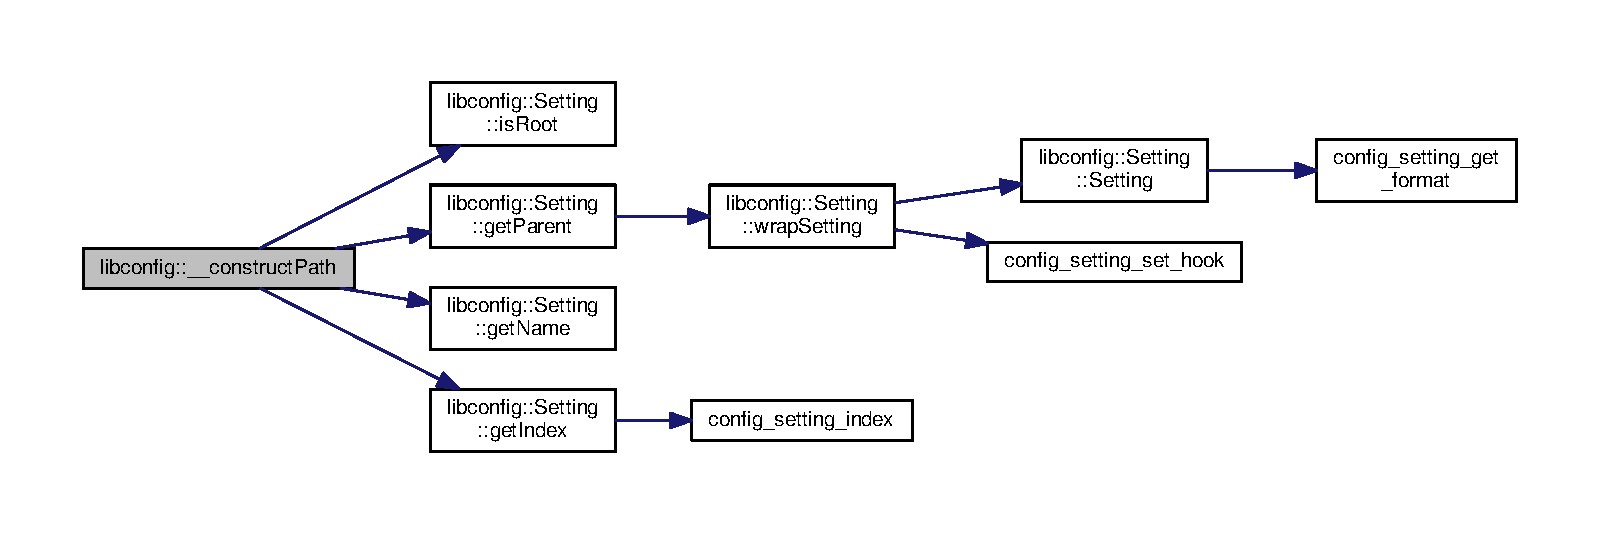
\includegraphics[width=350pt]{namespacelibconfig_ac6ddf54284dd0e8344d0e64a61cf9f17_cgraph}
\end{center}
\end{figure}




Here is the caller graph for this function\-:\nopagebreak
\begin{figure}[H]
\begin{center}
\leavevmode
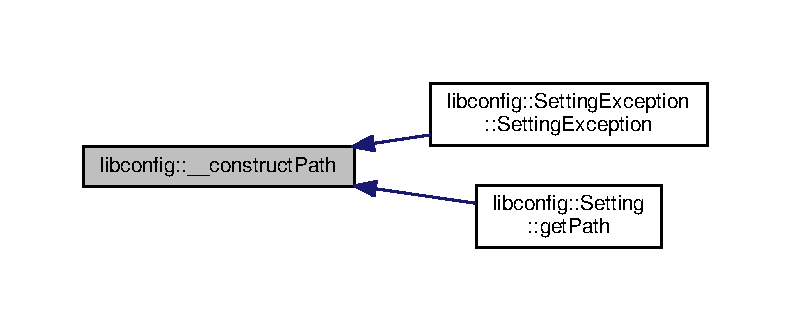
\includegraphics[width=350pt]{namespacelibconfig_ac6ddf54284dd0e8344d0e64a61cf9f17_icgraph}
\end{center}
\end{figure}


\hypertarget{namespacelibconfig_a8e110477bf88dac91c60df3cc4e7eebe}{\index{libconfig@{libconfig}!\-\_\-\-\_\-to\-Type\-Code@{\-\_\-\-\_\-to\-Type\-Code}}
\index{\-\_\-\-\_\-to\-Type\-Code@{\-\_\-\-\_\-to\-Type\-Code}!libconfig@{libconfig}}
\subsubsection[{\-\_\-\-\_\-to\-Type\-Code}]{\setlength{\rightskip}{0pt plus 5cm}static int libconfig\-::\-\_\-\-\_\-to\-Type\-Code (
\begin{DoxyParamCaption}
\item[{Setting\-::\-Type}]{type}
\end{DoxyParamCaption}
)\hspace{0.3cm}{\ttfamily [static]}}}\label{namespacelibconfig_a8e110477bf88dac91c60df3cc4e7eebe}


Here is the caller graph for this function\-:\nopagebreak
\begin{figure}[H]
\begin{center}
\leavevmode
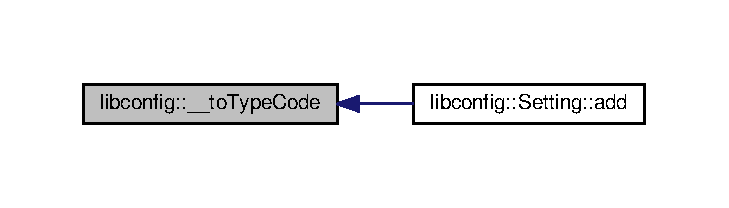
\includegraphics[width=350pt]{namespacelibconfig_a8e110477bf88dac91c60df3cc4e7eebe_icgraph}
\end{center}
\end{figure}



\hypertarget{namespacetld}{\section{tld Namespace Reference}
\label{namespacetld}\index{tld@{tld}}
}
\subsection*{Classes}
\begin{DoxyCompactItemize}
\item 
class \hyperlink{classtld_1_1Clustering}{Clustering}
\begin{DoxyCompactList}\small\item\em The clustering of detector cascade results. \end{DoxyCompactList}\item 
class \hyperlink{classtld_1_1DetectionResult}{Detection\-Result}
\begin{DoxyCompactList}\small\item\em The detection result. \end{DoxyCompactList}\item 
class \hyperlink{classtld_1_1DetectorCascade}{Detector\-Cascade}
\begin{DoxyCompactList}\small\item\em The detector cascade. \end{DoxyCompactList}\item 
class \hyperlink{classtld_1_1EnsembleClassifier}{Ensemble\-Classifier}
\begin{DoxyCompactList}\small\item\em The ensemble classifier. \end{DoxyCompactList}\item 
class \hyperlink{classtld_1_1ForegroundDetector}{Foreground\-Detector}
\begin{DoxyCompactList}\small\item\em The foreground detector. \end{DoxyCompactList}\item 
class \hyperlink{classtld_1_1MedianFlowTracker}{Median\-Flow\-Tracker}
\begin{DoxyCompactList}\small\item\em The median flow tracker (based on the forward-\/backward error). \end{DoxyCompactList}\item 
class \hyperlink{classtld_1_1NNClassifier}{N\-N\-Classifier}
\begin{DoxyCompactList}\small\item\em The nearest neighbor classifier. \end{DoxyCompactList}\item 
class \hyperlink{classtld_1_1NormalizedPatch}{Normalized\-Patch}
\begin{DoxyCompactList}\small\item\em The normalized patch (image). \end{DoxyCompactList}\item 
struct \hyperlink{structtld_1_1TldExportEntry}{Tld\-Export\-Entry}
\item 
class \hyperlink{classtld_1_1TLD}{T\-L\-D}
\begin{DoxyCompactList}\small\item\em The tracking lerning detector. \end{DoxyCompactList}\item 
class \hyperlink{classtld_1_1VarianceFilter}{Variance\-Filter}
\begin{DoxyCompactList}\small\item\em The variance filter. \end{DoxyCompactList}\item 
class \hyperlink{classtld_1_1Config}{Config}
\begin{DoxyCompactList}\small\item\em \hyperlink{classtld_1_1Config}{Config} is used to configure the program by cli and/or by a config file. \end{DoxyCompactList}\item 
class \hyperlink{classtld_1_1Gui}{Gui}
\begin{DoxyCompactList}\small\item\em Graphical user interface. \end{DoxyCompactList}\item 
class \hyperlink{classtld_1_1Settings}{Settings}
\begin{DoxyCompactList}\small\item\em In this class all settings are stored. \end{DoxyCompactList}\item 
class \hyperlink{classtld_1_1Trajectory}{Trajectory}
\begin{DoxyCompactList}\small\item\em Detection trajectory; a line which associates the last detections. The data is stored in 2 \char`\"{}shift registers\char`\"{}. \end{DoxyCompactList}\end{DoxyCompactItemize}
\subsection*{Functions}
\begin{DoxyCompactItemize}
\item 
void \hyperlink{namespacetld_ac0c16951370c978dee562ac3d3bd1554}{tld\-Rect\-To\-Points} (Cv\-Rect rect, Cv\-Point $\ast$p1, Cv\-Point $\ast$p2)
\begin{DoxyCompactList}\small\item\em Converts the rectangle to two points. \end{DoxyCompactList}\item 
void \hyperlink{namespacetld_a0c77964d9fc8756d176352372745a0ff}{tld\-Bounding\-Box\-To\-Points} (int $\ast$\hyperlink{namespacetld_aa5e13bbb9a53d3e9103d430b6113b08b}{bb}, Cv\-Point $\ast$p1, Cv\-Point $\ast$p2)
\begin{DoxyCompactList}\small\item\em Converts the array (size 4) to two points. \end{DoxyCompactList}\item 
void \hyperlink{namespacetld_a7facbe495da1f0e058c78b9b7dea412a}{tld\-Normalize\-Img} (const cv\-::\-Mat \&img, float $\ast$output)
\begin{DoxyCompactList}\small\item\em Returns mean-\/normalized patch, the image must be greyscale. \end{DoxyCompactList}\item 
Cv\-Rect \hyperlink{namespacetld_afd43d8a27c419d1f5da8718be917d4b5}{tld\-Boundary\-To\-Rect} (int $\ast$boundary)
\begin{DoxyCompactList}\small\item\em Creates new rectangle from boundary. \end{DoxyCompactList}\item 
void \hyperlink{namespacetld_a200bdf631ed45b6d0875996d2e4709f2}{tld\-Extract\-Sub\-Image} (const Mat \&img, Mat \&sub\-Image, Cv\-Rect rect)
\begin{DoxyCompactList}\small\item\em Extracts the subimage by the reactangle. \end{DoxyCompactList}\item 
void \hyperlink{namespacetld_a16fe2b016494fa66be611f723ed7bebc}{tld\-Extract\-Sub\-Image} (const cv\-::\-Mat \&img, cv\-::\-Mat \&sub\-Image, int $\ast$boundary)
\begin{DoxyCompactList}\small\item\em Extracts the subimage by the reactangle. \end{DoxyCompactList}\item 
void \hyperlink{namespacetld_ac965be65b1eae7ec666c3bfbe9da065e}{tld\-Extract\-Normalized\-Patch} (const cv\-::\-Mat \&img, int x, int y, int w, int h, float $\ast$output)
\begin{DoxyCompactList}\small\item\em Extracts normalized patch from the image by rectangle. \end{DoxyCompactList}\item 
void \hyperlink{namespacetld_a44b5f4d4d087d3369129bdc92e2a555a}{tld\-Extract\-Normalized\-Patch\-B\-B} (const cv\-::\-Mat \&img, int $\ast$boundary, float $\ast$output)
\begin{DoxyCompactList}\small\item\em Extracts normalized patch from the image by boundary (array). \end{DoxyCompactList}\item 
void \hyperlink{namespacetld_aa6c803037b38609e1fceadbb2ad8a75c}{tld\-Extract\-Normalized\-Patch\-Rect} (const cv\-::\-Mat \&img, cv\-::\-Rect $\ast$rect, float $\ast$output)
\begin{DoxyCompactList}\small\item\em Extracts normalized patch from the image by reactangle. \end{DoxyCompactList}\item 
float \hyperlink{namespacetld_a34eeb46b85efa569359847443ee96eba}{Calculate\-Mean} (float $\ast$value, int n)
\begin{DoxyCompactList}\small\item\em Calculates the mean value of array. \end{DoxyCompactList}\item 
float \hyperlink{namespacetld_a53d4a014fd3df2b3e8a3026a1c1768a7}{tld\-Calc\-Variance} (float $\ast$value, int n)
\begin{DoxyCompactList}\small\item\em Calculates the variance. \end{DoxyCompactList}\item 
float \hyperlink{namespacetld_a19776566a098d3b1fb15030e945a8c14}{tld\-B\-B\-Overlap} (int $\ast$bb1, int $\ast$bb2)
\begin{DoxyCompactList}\small\item\em Calculates the share overlap of two bounding boxes (the share the intersection area in the occupy area). \end{DoxyCompactList}\item 
void \hyperlink{namespacetld_a018caa7bf4a554814fe61a679a219489}{tld\-Overlap\-One} (int $\ast$windows, int num\-Windows, int index, std\-::vector$<$ int $>$ $\ast$indices, float $\ast$overlap)
\begin{DoxyCompactList}\small\item\em Calculates the share overlap of one window and the indexed windows (according). \end{DoxyCompactList}\item 
float \hyperlink{namespacetld_afdab54607fed863cdc408f72fd0f774b}{tld\-Overlap\-Rect\-Rect} (cv\-::\-Rect r1, cv\-::\-Rect r2)
\begin{DoxyCompactList}\small\item\em Calculates the share overlap of two rectangle (the share the intersection area in the occupy area). \end{DoxyCompactList}\item 
cv\-::\-Rect $\ast$ \hyperlink{namespacetld_aa09746d2aa3c9d71e4e0ba54d70d0e66}{tld\-Copy\-Rect} (cv\-::\-Rect $\ast$r)
\begin{DoxyCompactList}\small\item\em Creates the copy of rectangle. \end{DoxyCompactList}\item 
void \hyperlink{namespacetld_ae87c7dbe6b4da1e1923c42bec18caaf6}{tld\-Overlap\-Rect} (int $\ast$windows, int num\-Windows, cv\-::\-Rect $\ast$boundary, float $\ast$overlap)
\begin{DoxyCompactList}\small\item\em Calculates the share overlap of windows and the rectangle. \end{DoxyCompactList}\item 
void \hyperlink{namespacetld_aa9470de30170cb8b3f877dcae45df1b1}{tld\-Overlap} (int $\ast$windows, int num\-Windows, int $\ast$boundary, float $\ast$overlap)
\begin{DoxyCompactList}\small\item\em Calculates the share overlap of windows and the boundary. \end{DoxyCompactList}\item 
bool \hyperlink{namespacetld_acaf374df081816ecaf9079e200a8f5af}{tld\-Sort\-By\-Overlap\-Desc} (std\-::pair$<$ int, float $>$ bb1, std\-::pair$<$ int, float $>$ bb2)
\begin{DoxyCompactList}\small\item\em Checks whether the second parameter of one pair is more then the second parameter of other pair. \end{DoxyCompactList}\item 
int \hyperlink{namespacetld_a8b28e6d4868ad30e826a6248dd2ae7a0}{tld\-Is\-Inside} (int $\ast$bb1, int $\ast$bb2)
\begin{DoxyCompactList}\small\item\em Checks whether the one bouning box is completely inside the other. \end{DoxyCompactList}\item 
{\footnotesize template$<$class T1 , class T2 $>$ }\\void \hyperlink{namespacetld_a76d4a1c9344fcb821fda1f8c6ad587bc}{tld\-Convert\-B\-B} (T1 $\ast$src, T2 $\ast$dest)
\begin{DoxyCompactList}\small\item\em Converts the bouning box to other type. \end{DoxyCompactList}\item 
{\footnotesize template$<$class T $>$ }\\void \hyperlink{namespacetld_ac08655e901fb2ced507566217d4b5aca}{tld\-Copy\-B\-B} (T $\ast$src, T $\ast$dest)
\begin{DoxyCompactList}\small\item\em Copies the bouning box to the other. \end{DoxyCompactList}\item 
{\footnotesize template$<$class T $>$ }\\void \hyperlink{namespacetld_aefacde9f718a4102ac40901afa1b35f7}{tld\-Copy\-Boundary\-To\-Array} (T x, T y, T width, T height, T $\ast$array)
\begin{DoxyCompactList}\small\item\em Copies the boundary to the array (size 4). \end{DoxyCompactList}\item 
{\footnotesize template$<$class T $>$ }\\void \hyperlink{namespacetld_aff4c05bc28ae29c360be58460a56b579}{tld\-Extract\-Dims\-From\-Array} (T $\ast$boundary, T $\ast$x, T $\ast$y, T $\ast$width, T $\ast$height)
\begin{DoxyCompactList}\small\item\em Extracts the date from array (size 4). \end{DoxyCompactList}\item 
{\footnotesize template$<$class T $>$ }\\void \hyperlink{namespacetld_a18975268ebbf3daf5eaf46d30fd782e9}{tld\-Rect\-To\-Array} (cv\-::\-Rect rect, T $\ast$boundary)
\begin{DoxyCompactList}\small\item\em Converts the rectangle to array (size 4). \end{DoxyCompactList}\item 
{\footnotesize template$<$class T $>$ }\\cv\-::\-Rect \hyperlink{namespacetld_ad23d08bb67b847f43e2781a53f4af957}{tld\-Array\-To\-Rect} (T $\ast$boundary)
\begin{DoxyCompactList}\small\item\em Converts the array (size 4) to rectangle. \end{DoxyCompactList}\item 
void \hyperlink{namespacetld_a7699b7dc20502fc6d7c5c6c6cbd4be7b}{tld\-Extract\-Sub\-Image} (const cv\-::\-Mat \&img, cv\-::\-Mat \&sub\-Image, int x, int y, int w, int h)
\begin{DoxyCompactList}\small\item\em Extracts the subimage by the reactangle. \end{DoxyCompactList}\item 
float \hyperlink{namespacetld_ac0065f4088098aca6e1edd49b2b0f9d3}{tld\-Calc\-Mean} (float $\ast$value, int n)
\begin{DoxyCompactList}\small\item\em It isn't realized. \end{DoxyCompactList}\item 
int \hyperlink{namespacetld_a5b279570cd95fb0067a41b5a222e2642}{getopt} (int argc, char $\ast$$\ast$argv, char $\ast$opts)
\item 
static void \hyperlink{namespacetld_aed141e469725fa20f8828efbe29e57f1}{mouse\-Handler} (int event, int x, int y, int flags, void $\ast$param)
\item 
int \hyperlink{namespacetld_a75cd208f8053ece69d5d7de9c2ed33fd}{get\-B\-B\-From\-User} (Ipl\-Image $\ast$img, Cv\-Rect \&rect, \hyperlink{classtld_1_1Gui}{Gui} $\ast$gui)
\begin{DoxyCompactList}\small\item\em Gets a bounding box from the user. \end{DoxyCompactList}\end{DoxyCompactItemize}
\subsection*{Variables}
\begin{DoxyCompactItemize}
\item 
static const int \hyperlink{namespacetld_ad0458a97a7973a088840e7917515c6ae}{T\-L\-D\-\_\-\-W\-I\-N\-D\-O\-W\-\_\-\-S\-I\-Z\-E} = 5
\begin{DoxyCompactList}\small\item\em the size of array, defining the window \end{DoxyCompactList}\item 
static const int \hyperlink{namespacetld_a7a647c1eaeda30086f4519b611db4e71}{T\-L\-D\-\_\-\-W\-I\-N\-D\-O\-W\-\_\-\-O\-F\-F\-S\-E\-T\-\_\-\-S\-I\-Z\-E} = 6
\begin{DoxyCompactList}\small\item\em the size of array, defining the window offset \end{DoxyCompactList}\item 
static char \hyperlink{namespacetld_a17f0b1eb181c0395a541e031b203040a}{help\-\_\-text} \mbox{[}$\,$\mbox{]}
\item 
int \hyperlink{namespacetld_a6e180d5067af278cc277ae9c6f7507c1}{opterr} = 1
\item 
int \hyperlink{namespacetld_ab8c5a378ef03678c537edc84a15abc22}{optind} = 1
\item 
int \hyperlink{namespacetld_a6d6bd80732b9f396bc03e5f2c5cf30f8}{optopt}
\item 
char $\ast$ \hyperlink{namespacetld_a1bbc7d3201a2ef41da5495e0e48cfd2e}{optarg}
\item 
static string \hyperlink{namespacetld_ad1bfc03770cc333da8a972ab7d35c246}{window\-\_\-name}
\item 
static Cv\-Font \hyperlink{namespacetld_a16a44df30fb791b45dd103ba1541fb67}{font}
\item 
static Ipl\-Image $\ast$ \hyperlink{namespacetld_a32bc4295eda098201cd336e2d2f1e217}{img0}
\item 
static Ipl\-Image $\ast$ \hyperlink{namespacetld_ac832a3e8122e594c1c5321935cbc2639}{img1}
\item 
static Cv\-Point \hyperlink{namespacetld_a680868c3e5a47352c5353897519636d4}{point}
\item 
static Cv\-Rect $\ast$ \hyperlink{namespacetld_aa5e13bbb9a53d3e9103d430b6113b08b}{bb}
\item 
static int \hyperlink{namespacetld_a7cfa165f34457693b8898cfa78e51945}{drag} = 0
\end{DoxyCompactItemize}


\subsection{Detailed Description}
\begin{DoxyAuthor}{Author}
Clemens Korner 
\end{DoxyAuthor}


\subsection{Function Documentation}
\hypertarget{namespacetld_a34eeb46b85efa569359847443ee96eba}{\index{tld@{tld}!Calculate\-Mean@{Calculate\-Mean}}
\index{Calculate\-Mean@{Calculate\-Mean}!tld@{tld}}
\subsubsection[{Calculate\-Mean}]{\setlength{\rightskip}{0pt plus 5cm}float tld\-::\-Calculate\-Mean (
\begin{DoxyParamCaption}
\item[{float $\ast$}]{value, }
\item[{int}]{n}
\end{DoxyParamCaption}
)}}\label{namespacetld_a34eeb46b85efa569359847443ee96eba}


Calculates the mean value of array. 


\begin{DoxyParams}{Parameters}
{\em value} & the array \\
\hline
{\em n} & the size of array \\
\hline
\end{DoxyParams}
\begin{DoxyReturn}{Returns}
float the mean value 
\end{DoxyReturn}


Here is the caller graph for this function\-:\nopagebreak
\begin{figure}[H]
\begin{center}
\leavevmode
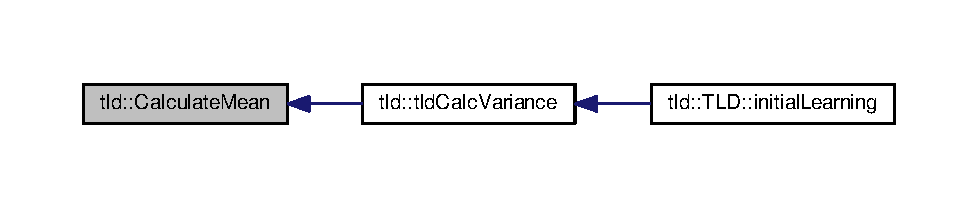
\includegraphics[width=350pt]{namespacetld_a34eeb46b85efa569359847443ee96eba_icgraph}
\end{center}
\end{figure}


\hypertarget{namespacetld_a75cd208f8053ece69d5d7de9c2ed33fd}{\index{tld@{tld}!get\-B\-B\-From\-User@{get\-B\-B\-From\-User}}
\index{get\-B\-B\-From\-User@{get\-B\-B\-From\-User}!tld@{tld}}
\subsubsection[{get\-B\-B\-From\-User}]{\setlength{\rightskip}{0pt plus 5cm}int tld\-::get\-B\-B\-From\-User (
\begin{DoxyParamCaption}
\item[{Ipl\-Image $\ast$}]{img, }
\item[{Cv\-Rect \&}]{rect, }
\item[{Gui $\ast$}]{gui}
\end{DoxyParamCaption}
)}}\label{namespacetld_a75cd208f8053ece69d5d7de9c2ed33fd}


Gets a bounding box from the user. 


\begin{DoxyParams}{Parameters}
{\em img} & image to display \\
\hline
{\em rect} & Cv\-Rect containing the coordinates of the bounding box \\
\hline
{\em gui} & initialized gui \\
\hline
\end{DoxyParams}
\begin{DoxyReturn}{Returns}
P\-R\-O\-G\-R\-A\-M\-\_\-\-E\-X\-I\-T if 'q' or 'Q' pressed, S\-U\-C\-C\-E\-S\-S if everything went right 
\end{DoxyReturn}


Here is the call graph for this function\-:\nopagebreak
\begin{figure}[H]
\begin{center}
\leavevmode
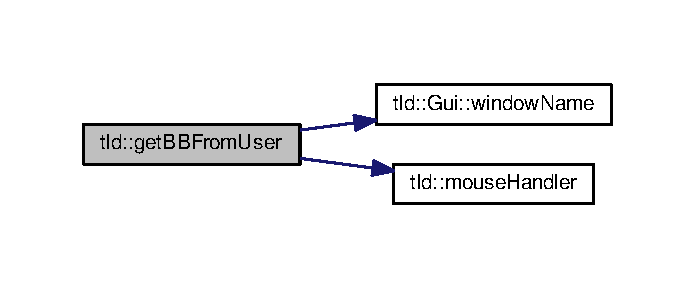
\includegraphics[width=334pt]{namespacetld_a75cd208f8053ece69d5d7de9c2ed33fd_cgraph}
\end{center}
\end{figure}




Here is the caller graph for this function\-:\nopagebreak
\begin{figure}[H]
\begin{center}
\leavevmode
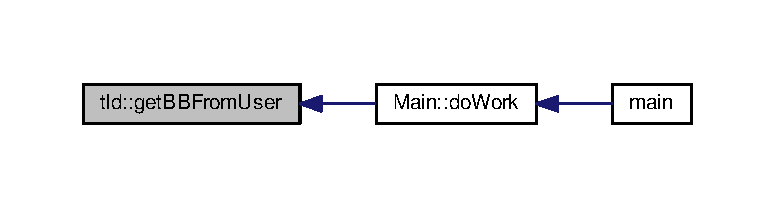
\includegraphics[width=350pt]{namespacetld_a75cd208f8053ece69d5d7de9c2ed33fd_icgraph}
\end{center}
\end{figure}


\hypertarget{namespacetld_a5b279570cd95fb0067a41b5a222e2642}{\index{tld@{tld}!getopt@{getopt}}
\index{getopt@{getopt}!tld@{tld}}
\subsubsection[{getopt}]{\setlength{\rightskip}{0pt plus 5cm}int tld\-::getopt (
\begin{DoxyParamCaption}
\item[{int}]{argc, }
\item[{char $\ast$$\ast$}]{argv, }
\item[{char $\ast$}]{opts}
\end{DoxyParamCaption}
)}}\label{namespacetld_a5b279570cd95fb0067a41b5a222e2642}


Here is the caller graph for this function\-:\nopagebreak
\begin{figure}[H]
\begin{center}
\leavevmode
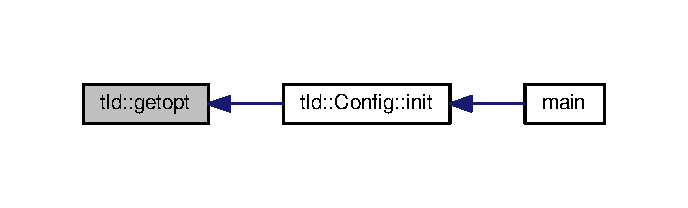
\includegraphics[width=330pt]{namespacetld_a5b279570cd95fb0067a41b5a222e2642_icgraph}
\end{center}
\end{figure}


\hypertarget{namespacetld_aed141e469725fa20f8828efbe29e57f1}{\index{tld@{tld}!mouse\-Handler@{mouse\-Handler}}
\index{mouse\-Handler@{mouse\-Handler}!tld@{tld}}
\subsubsection[{mouse\-Handler}]{\setlength{\rightskip}{0pt plus 5cm}static void tld\-::mouse\-Handler (
\begin{DoxyParamCaption}
\item[{int}]{event, }
\item[{int}]{x, }
\item[{int}]{y, }
\item[{int}]{flags, }
\item[{void $\ast$}]{param}
\end{DoxyParamCaption}
)\hspace{0.3cm}{\ttfamily [static]}}}\label{namespacetld_aed141e469725fa20f8828efbe29e57f1}


Here is the caller graph for this function\-:\nopagebreak
\begin{figure}[H]
\begin{center}
\leavevmode
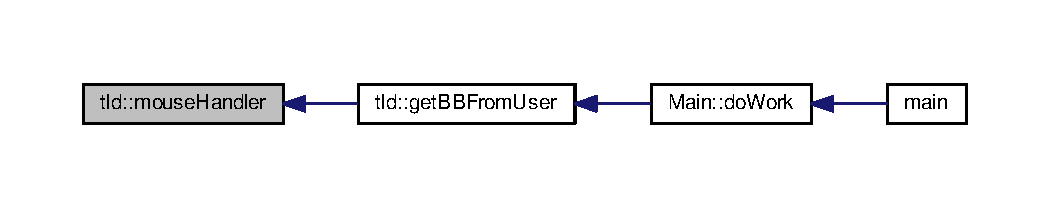
\includegraphics[width=350pt]{namespacetld_aed141e469725fa20f8828efbe29e57f1_icgraph}
\end{center}
\end{figure}


\hypertarget{namespacetld_ad23d08bb67b847f43e2781a53f4af957}{\index{tld@{tld}!tld\-Array\-To\-Rect@{tld\-Array\-To\-Rect}}
\index{tld\-Array\-To\-Rect@{tld\-Array\-To\-Rect}!tld@{tld}}
\subsubsection[{tld\-Array\-To\-Rect}]{\setlength{\rightskip}{0pt plus 5cm}template$<$class T $>$ cv\-::\-Rect tld\-::tld\-Array\-To\-Rect (
\begin{DoxyParamCaption}
\item[{T $\ast$}]{boundary}
\end{DoxyParamCaption}
)}}\label{namespacetld_ad23d08bb67b847f43e2781a53f4af957}


Converts the array (size 4) to rectangle. 


\begin{DoxyParams}{Parameters}
{\em boundary} & the array \\
\hline
\end{DoxyParams}
\begin{DoxyReturn}{Returns}
the rectangle 
\end{DoxyReturn}


Here is the caller graph for this function\-:\nopagebreak
\begin{figure}[H]
\begin{center}
\leavevmode
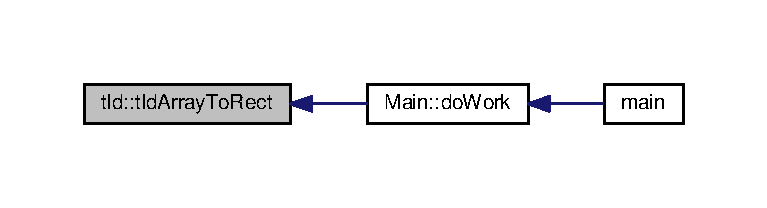
\includegraphics[width=350pt]{namespacetld_ad23d08bb67b847f43e2781a53f4af957_icgraph}
\end{center}
\end{figure}


\hypertarget{namespacetld_a19776566a098d3b1fb15030e945a8c14}{\index{tld@{tld}!tld\-B\-B\-Overlap@{tld\-B\-B\-Overlap}}
\index{tld\-B\-B\-Overlap@{tld\-B\-B\-Overlap}!tld@{tld}}
\subsubsection[{tld\-B\-B\-Overlap}]{\setlength{\rightskip}{0pt plus 5cm}float tld\-::tld\-B\-B\-Overlap (
\begin{DoxyParamCaption}
\item[{int $\ast$}]{bb1, }
\item[{int $\ast$}]{bb2}
\end{DoxyParamCaption}
)}}\label{namespacetld_a19776566a098d3b1fb15030e945a8c14}


Calculates the share overlap of two bounding boxes (the share the intersection area in the occupy area). 


\begin{DoxyParams}{Parameters}
{\em bb1} & the one bounding box \\
\hline
{\em bb2} & the two bounding box \\
\hline
\end{DoxyParams}
\begin{DoxyReturn}{Returns}
the share overlap(0 to 1) 
\end{DoxyReturn}


Here is the caller graph for this function\-:\nopagebreak
\begin{figure}[H]
\begin{center}
\leavevmode
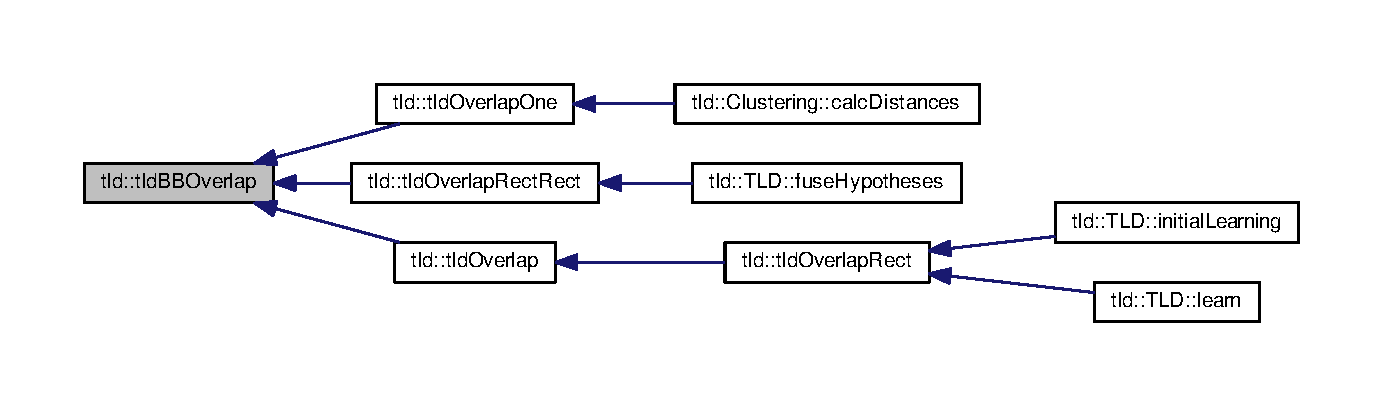
\includegraphics[width=350pt]{namespacetld_a19776566a098d3b1fb15030e945a8c14_icgraph}
\end{center}
\end{figure}


\hypertarget{namespacetld_afd43d8a27c419d1f5da8718be917d4b5}{\index{tld@{tld}!tld\-Boundary\-To\-Rect@{tld\-Boundary\-To\-Rect}}
\index{tld\-Boundary\-To\-Rect@{tld\-Boundary\-To\-Rect}!tld@{tld}}
\subsubsection[{tld\-Boundary\-To\-Rect}]{\setlength{\rightskip}{0pt plus 5cm}Cv\-Rect tld\-::tld\-Boundary\-To\-Rect (
\begin{DoxyParamCaption}
\item[{int $\ast$}]{boundary}
\end{DoxyParamCaption}
)}}\label{namespacetld_afd43d8a27c419d1f5da8718be917d4b5}


Creates new rectangle from boundary. 


\begin{DoxyParams}{Parameters}
{\em boundary} & the array (size 4) \\
\hline
\end{DoxyParams}
\begin{DoxyReturn}{Returns}
the rectangle 
\end{DoxyReturn}


Here is the caller graph for this function\-:\nopagebreak
\begin{figure}[H]
\begin{center}
\leavevmode
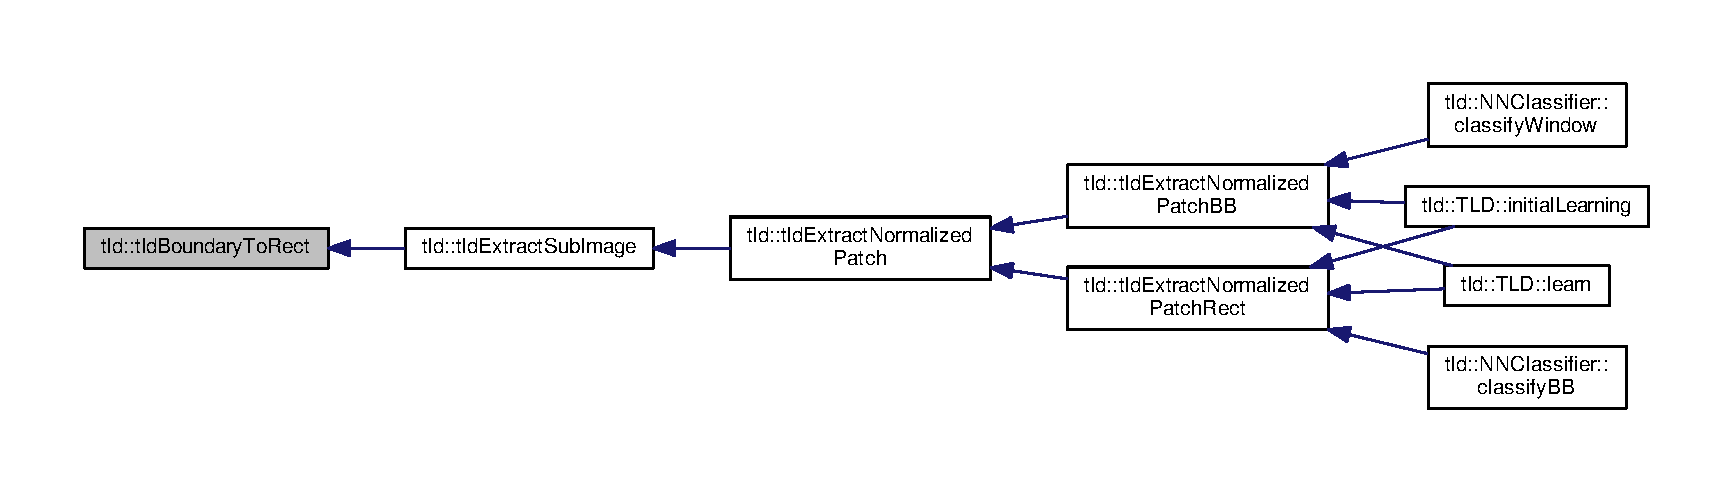
\includegraphics[width=350pt]{namespacetld_afd43d8a27c419d1f5da8718be917d4b5_icgraph}
\end{center}
\end{figure}


\hypertarget{namespacetld_a0c77964d9fc8756d176352372745a0ff}{\index{tld@{tld}!tld\-Bounding\-Box\-To\-Points@{tld\-Bounding\-Box\-To\-Points}}
\index{tld\-Bounding\-Box\-To\-Points@{tld\-Bounding\-Box\-To\-Points}!tld@{tld}}
\subsubsection[{tld\-Bounding\-Box\-To\-Points}]{\setlength{\rightskip}{0pt plus 5cm}void tld\-::tld\-Bounding\-Box\-To\-Points (
\begin{DoxyParamCaption}
\item[{int $\ast$}]{bb, }
\item[{Cv\-Point $\ast$}]{p1, }
\item[{Cv\-Point $\ast$}]{p2}
\end{DoxyParamCaption}
)}}\label{namespacetld_a0c77964d9fc8756d176352372745a0ff}


Converts the array (size 4) to two points. 


\begin{DoxyParams}{Parameters}
{\em bb} & the array (bouning box) \\
\hline
{\em p1} & the left top point \\
\hline
{\em p2} & the right bottom point \\
\hline
\end{DoxyParams}
\hypertarget{namespacetld_ac0065f4088098aca6e1edd49b2b0f9d3}{\index{tld@{tld}!tld\-Calc\-Mean@{tld\-Calc\-Mean}}
\index{tld\-Calc\-Mean@{tld\-Calc\-Mean}!tld@{tld}}
\subsubsection[{tld\-Calc\-Mean}]{\setlength{\rightskip}{0pt plus 5cm}float tld\-::tld\-Calc\-Mean (
\begin{DoxyParamCaption}
\item[{float $\ast$}]{value, }
\item[{int}]{n}
\end{DoxyParamCaption}
)}}\label{namespacetld_ac0065f4088098aca6e1edd49b2b0f9d3}


It isn't realized. 


\begin{DoxyParams}{Parameters}
{\em value} & \\
\hline
{\em n} & \\
\hline
\end{DoxyParams}
\begin{DoxyReturn}{Returns}
float 
\end{DoxyReturn}
\hypertarget{namespacetld_a53d4a014fd3df2b3e8a3026a1c1768a7}{\index{tld@{tld}!tld\-Calc\-Variance@{tld\-Calc\-Variance}}
\index{tld\-Calc\-Variance@{tld\-Calc\-Variance}!tld@{tld}}
\subsubsection[{tld\-Calc\-Variance}]{\setlength{\rightskip}{0pt plus 5cm}float tld\-::tld\-Calc\-Variance (
\begin{DoxyParamCaption}
\item[{float $\ast$}]{value, }
\item[{int}]{n}
\end{DoxyParamCaption}
)}}\label{namespacetld_a53d4a014fd3df2b3e8a3026a1c1768a7}


Calculates the variance. 


\begin{DoxyParams}{Parameters}
{\em value} & the array \\
\hline
{\em n} & the size of array \\
\hline
\end{DoxyParams}
\begin{DoxyReturn}{Returns}
the value of variance 
\end{DoxyReturn}


Here is the call graph for this function\-:\nopagebreak
\begin{figure}[H]
\begin{center}
\leavevmode
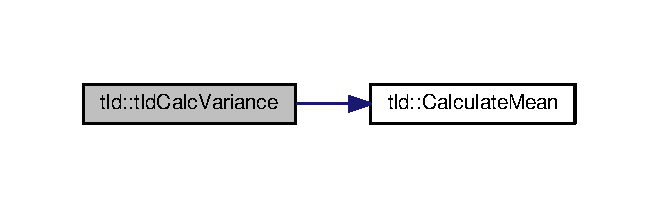
\includegraphics[width=316pt]{namespacetld_a53d4a014fd3df2b3e8a3026a1c1768a7_cgraph}
\end{center}
\end{figure}




Here is the caller graph for this function\-:\nopagebreak
\begin{figure}[H]
\begin{center}
\leavevmode
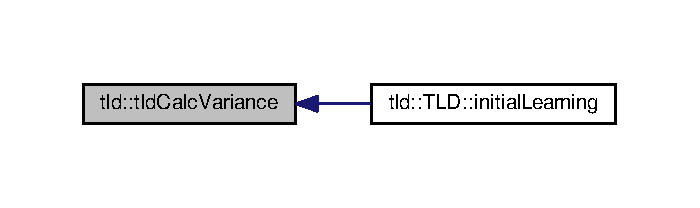
\includegraphics[width=336pt]{namespacetld_a53d4a014fd3df2b3e8a3026a1c1768a7_icgraph}
\end{center}
\end{figure}


\hypertarget{namespacetld_a76d4a1c9344fcb821fda1f8c6ad587bc}{\index{tld@{tld}!tld\-Convert\-B\-B@{tld\-Convert\-B\-B}}
\index{tld\-Convert\-B\-B@{tld\-Convert\-B\-B}!tld@{tld}}
\subsubsection[{tld\-Convert\-B\-B}]{\setlength{\rightskip}{0pt plus 5cm}template$<$class T1 , class T2 $>$ void tld\-::tld\-Convert\-B\-B (
\begin{DoxyParamCaption}
\item[{T1 $\ast$}]{src, }
\item[{T2 $\ast$}]{dest}
\end{DoxyParamCaption}
)}}\label{namespacetld_a76d4a1c9344fcb821fda1f8c6ad587bc}


Converts the bouning box to other type. 


\begin{DoxyParams}{Parameters}
{\em src} & the source bouning box \\
\hline
{\em dest} & the destination bouning box \\
\hline
\end{DoxyParams}
\hypertarget{namespacetld_ac08655e901fb2ced507566217d4b5aca}{\index{tld@{tld}!tld\-Copy\-B\-B@{tld\-Copy\-B\-B}}
\index{tld\-Copy\-B\-B@{tld\-Copy\-B\-B}!tld@{tld}}
\subsubsection[{tld\-Copy\-B\-B}]{\setlength{\rightskip}{0pt plus 5cm}template$<$class T $>$ void tld\-::tld\-Copy\-B\-B (
\begin{DoxyParamCaption}
\item[{T $\ast$}]{src, }
\item[{T $\ast$}]{dest}
\end{DoxyParamCaption}
)}}\label{namespacetld_ac08655e901fb2ced507566217d4b5aca}


Copies the bouning box to the other. 


\begin{DoxyParams}{Parameters}
{\em src} & the source bouning box \\
\hline
{\em dest} & the destination bouning box \\
\hline
\end{DoxyParams}
\hypertarget{namespacetld_aefacde9f718a4102ac40901afa1b35f7}{\index{tld@{tld}!tld\-Copy\-Boundary\-To\-Array@{tld\-Copy\-Boundary\-To\-Array}}
\index{tld\-Copy\-Boundary\-To\-Array@{tld\-Copy\-Boundary\-To\-Array}!tld@{tld}}
\subsubsection[{tld\-Copy\-Boundary\-To\-Array}]{\setlength{\rightskip}{0pt plus 5cm}template$<$class T $>$ void tld\-::tld\-Copy\-Boundary\-To\-Array (
\begin{DoxyParamCaption}
\item[{T}]{x, }
\item[{T}]{y, }
\item[{T}]{width, }
\item[{T}]{height, }
\item[{T $\ast$}]{array}
\end{DoxyParamCaption}
)}}\label{namespacetld_aefacde9f718a4102ac40901afa1b35f7}


Copies the boundary to the array (size 4). 


\begin{DoxyParams}{Parameters}
{\em x} & the x coordinate of the left top point of boundary \\
\hline
{\em y} & the y coordinate of the left top point of boundary \\
\hline
{\em width} & the width boundary \\
\hline
{\em height} & the height boundary \\
\hline
{\em array} & the destination array \\
\hline
\end{DoxyParams}
\hypertarget{namespacetld_aa09746d2aa3c9d71e4e0ba54d70d0e66}{\index{tld@{tld}!tld\-Copy\-Rect@{tld\-Copy\-Rect}}
\index{tld\-Copy\-Rect@{tld\-Copy\-Rect}!tld@{tld}}
\subsubsection[{tld\-Copy\-Rect}]{\setlength{\rightskip}{0pt plus 5cm}cv\-::\-Rect $\ast$ tld\-::tld\-Copy\-Rect (
\begin{DoxyParamCaption}
\item[{cv\-::\-Rect $\ast$}]{r}
\end{DoxyParamCaption}
)}}\label{namespacetld_aa09746d2aa3c9d71e4e0ba54d70d0e66}


Creates the copy of rectangle. 


\begin{DoxyParams}{Parameters}
{\em r} & the source rectangle \\
\hline
\end{DoxyParams}
\begin{DoxyReturn}{Returns}
the new rectangle 
\end{DoxyReturn}


Here is the caller graph for this function\-:\nopagebreak
\begin{figure}[H]
\begin{center}
\leavevmode
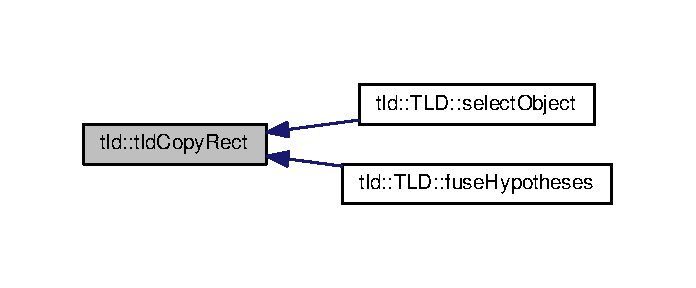
\includegraphics[width=334pt]{namespacetld_aa09746d2aa3c9d71e4e0ba54d70d0e66_icgraph}
\end{center}
\end{figure}


\hypertarget{namespacetld_aff4c05bc28ae29c360be58460a56b579}{\index{tld@{tld}!tld\-Extract\-Dims\-From\-Array@{tld\-Extract\-Dims\-From\-Array}}
\index{tld\-Extract\-Dims\-From\-Array@{tld\-Extract\-Dims\-From\-Array}!tld@{tld}}
\subsubsection[{tld\-Extract\-Dims\-From\-Array}]{\setlength{\rightskip}{0pt plus 5cm}template$<$class T $>$ void tld\-::tld\-Extract\-Dims\-From\-Array (
\begin{DoxyParamCaption}
\item[{T $\ast$}]{boundary, }
\item[{T $\ast$}]{x, }
\item[{T $\ast$}]{y, }
\item[{T $\ast$}]{width, }
\item[{T $\ast$}]{height}
\end{DoxyParamCaption}
)}}\label{namespacetld_aff4c05bc28ae29c360be58460a56b579}


Extracts the date from array (size 4). 


\begin{DoxyParams}{Parameters}
{\em boundary} & the source array.\-comparing \\
\hline
{\em x} & the 0 element of array \\
\hline
{\em y} & the 1 element of array \\
\hline
{\em width} & the 2 element of array \\
\hline
{\em height} & the 3 element of array \\
\hline
\end{DoxyParams}


Here is the caller graph for this function\-:\nopagebreak
\begin{figure}[H]
\begin{center}
\leavevmode
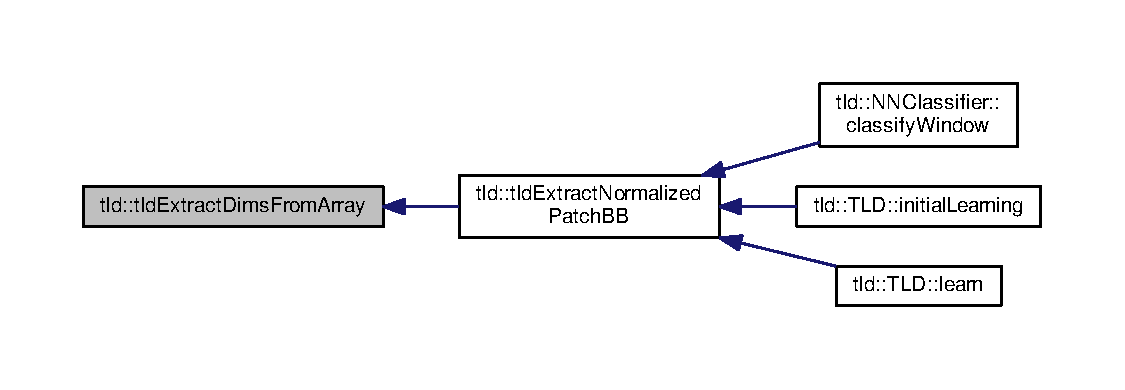
\includegraphics[width=350pt]{namespacetld_aff4c05bc28ae29c360be58460a56b579_icgraph}
\end{center}
\end{figure}


\hypertarget{namespacetld_ac965be65b1eae7ec666c3bfbe9da065e}{\index{tld@{tld}!tld\-Extract\-Normalized\-Patch@{tld\-Extract\-Normalized\-Patch}}
\index{tld\-Extract\-Normalized\-Patch@{tld\-Extract\-Normalized\-Patch}!tld@{tld}}
\subsubsection[{tld\-Extract\-Normalized\-Patch}]{\setlength{\rightskip}{0pt plus 5cm}void tld\-::tld\-Extract\-Normalized\-Patch (
\begin{DoxyParamCaption}
\item[{const cv\-::\-Mat \&}]{img, }
\item[{int}]{x, }
\item[{int}]{y, }
\item[{int}]{w, }
\item[{int}]{h, }
\item[{float $\ast$}]{output}
\end{DoxyParamCaption}
)}}\label{namespacetld_ac965be65b1eae7ec666c3bfbe9da065e}


Extracts normalized patch from the image by rectangle. 


\begin{DoxyParams}{Parameters}
{\em img} & the source image \\
\hline
{\em x} & the x coordinate of the left top point of reactangle \\
\hline
{\em y} & the y coordinate of the left top point of reactangle \\
\hline
{\em w} & the width reactangle \\
\hline
{\em h} & the height reactangle \\
\hline
{\em output} & the destination array (patch) \\
\hline
\end{DoxyParams}


Here is the call graph for this function\-:\nopagebreak
\begin{figure}[H]
\begin{center}
\leavevmode
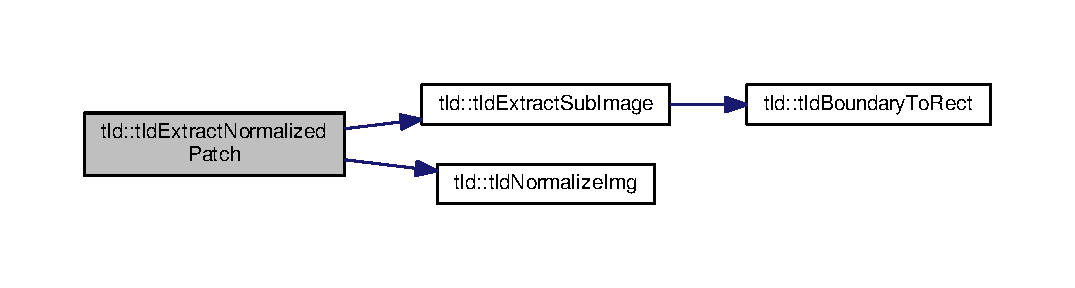
\includegraphics[width=350pt]{namespacetld_ac965be65b1eae7ec666c3bfbe9da065e_cgraph}
\end{center}
\end{figure}




Here is the caller graph for this function\-:\nopagebreak
\begin{figure}[H]
\begin{center}
\leavevmode
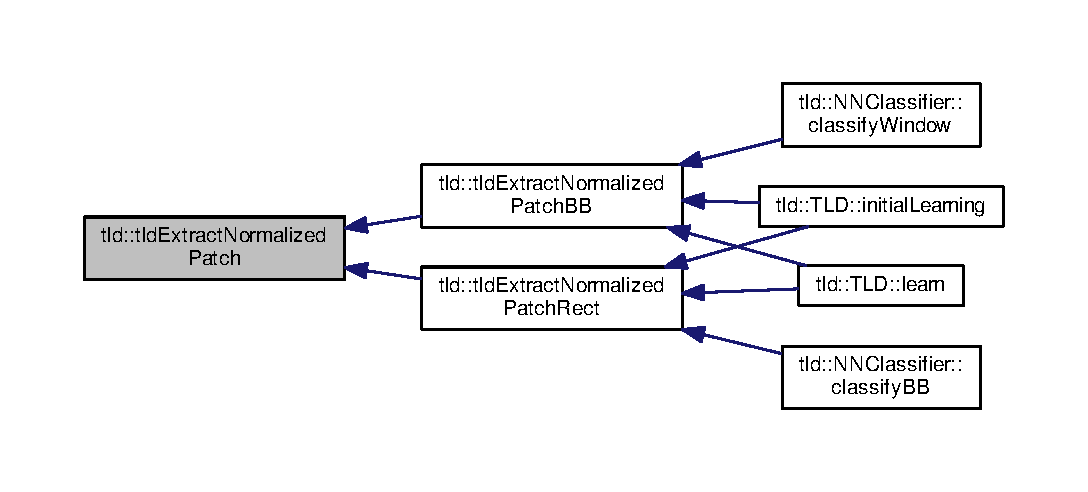
\includegraphics[width=350pt]{namespacetld_ac965be65b1eae7ec666c3bfbe9da065e_icgraph}
\end{center}
\end{figure}


\hypertarget{namespacetld_a44b5f4d4d087d3369129bdc92e2a555a}{\index{tld@{tld}!tld\-Extract\-Normalized\-Patch\-B\-B@{tld\-Extract\-Normalized\-Patch\-B\-B}}
\index{tld\-Extract\-Normalized\-Patch\-B\-B@{tld\-Extract\-Normalized\-Patch\-B\-B}!tld@{tld}}
\subsubsection[{tld\-Extract\-Normalized\-Patch\-B\-B}]{\setlength{\rightskip}{0pt plus 5cm}void tld\-::tld\-Extract\-Normalized\-Patch\-B\-B (
\begin{DoxyParamCaption}
\item[{const cv\-::\-Mat \&}]{img, }
\item[{int $\ast$}]{boundary, }
\item[{float $\ast$}]{output}
\end{DoxyParamCaption}
)}}\label{namespacetld_a44b5f4d4d087d3369129bdc92e2a555a}


Extracts normalized patch from the image by boundary (array). 


\begin{DoxyParams}{Parameters}
{\em img} & the source image \\
\hline
{\em boundary} & the array \\
\hline
{\em output} & the destination array (patch) \\
\hline
\end{DoxyParams}


Here is the call graph for this function\-:\nopagebreak
\begin{figure}[H]
\begin{center}
\leavevmode
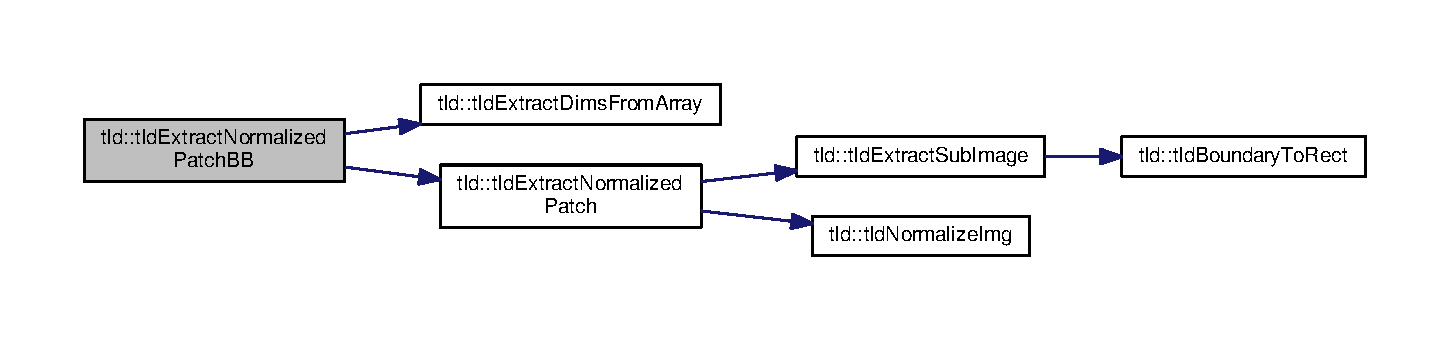
\includegraphics[width=350pt]{namespacetld_a44b5f4d4d087d3369129bdc92e2a555a_cgraph}
\end{center}
\end{figure}




Here is the caller graph for this function\-:\nopagebreak
\begin{figure}[H]
\begin{center}
\leavevmode
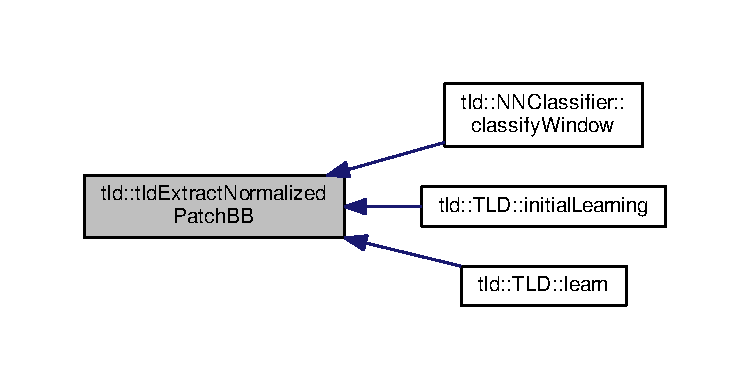
\includegraphics[width=350pt]{namespacetld_a44b5f4d4d087d3369129bdc92e2a555a_icgraph}
\end{center}
\end{figure}


\hypertarget{namespacetld_aa6c803037b38609e1fceadbb2ad8a75c}{\index{tld@{tld}!tld\-Extract\-Normalized\-Patch\-Rect@{tld\-Extract\-Normalized\-Patch\-Rect}}
\index{tld\-Extract\-Normalized\-Patch\-Rect@{tld\-Extract\-Normalized\-Patch\-Rect}!tld@{tld}}
\subsubsection[{tld\-Extract\-Normalized\-Patch\-Rect}]{\setlength{\rightskip}{0pt plus 5cm}void tld\-::tld\-Extract\-Normalized\-Patch\-Rect (
\begin{DoxyParamCaption}
\item[{const cv\-::\-Mat \&}]{img, }
\item[{cv\-::\-Rect $\ast$}]{rect, }
\item[{float $\ast$}]{output}
\end{DoxyParamCaption}
)}}\label{namespacetld_aa6c803037b38609e1fceadbb2ad8a75c}


Extracts normalized patch from the image by reactangle. 


\begin{DoxyParams}{Parameters}
{\em img} & the source image \\
\hline
{\em rect} & the rectangle \\
\hline
{\em output} & the destination array (patch) \\
\hline
\end{DoxyParams}


Here is the call graph for this function\-:\nopagebreak
\begin{figure}[H]
\begin{center}
\leavevmode
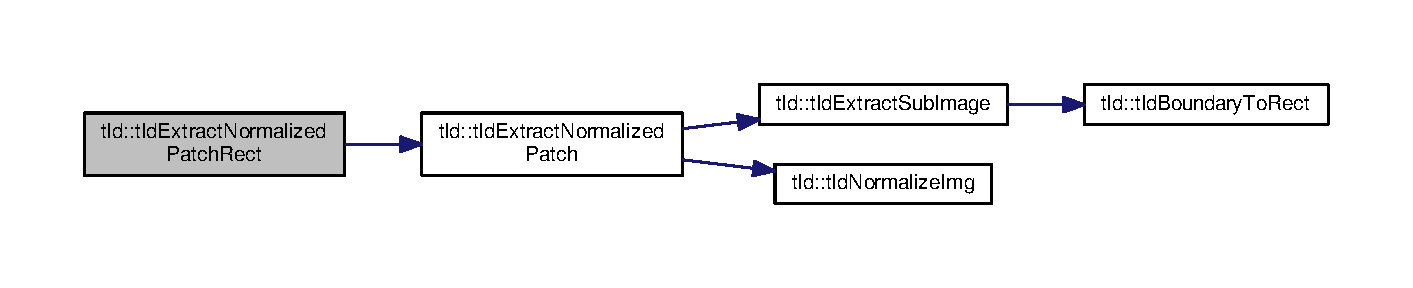
\includegraphics[width=350pt]{namespacetld_aa6c803037b38609e1fceadbb2ad8a75c_cgraph}
\end{center}
\end{figure}




Here is the caller graph for this function\-:\nopagebreak
\begin{figure}[H]
\begin{center}
\leavevmode
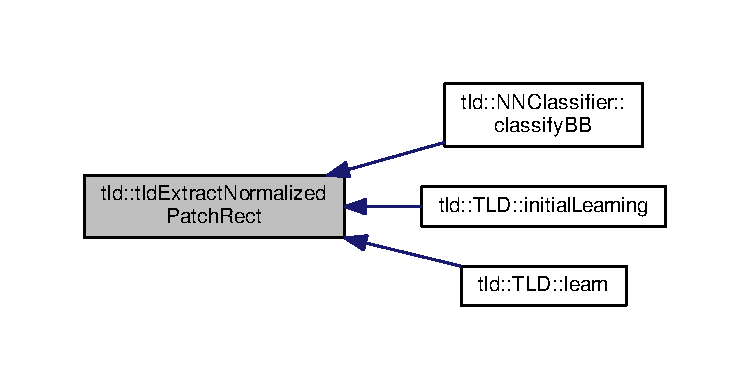
\includegraphics[width=350pt]{namespacetld_aa6c803037b38609e1fceadbb2ad8a75c_icgraph}
\end{center}
\end{figure}


\hypertarget{namespacetld_a200bdf631ed45b6d0875996d2e4709f2}{\index{tld@{tld}!tld\-Extract\-Sub\-Image@{tld\-Extract\-Sub\-Image}}
\index{tld\-Extract\-Sub\-Image@{tld\-Extract\-Sub\-Image}!tld@{tld}}
\subsubsection[{tld\-Extract\-Sub\-Image}]{\setlength{\rightskip}{0pt plus 5cm}void tld\-::tld\-Extract\-Sub\-Image (
\begin{DoxyParamCaption}
\item[{const Mat \&}]{img, }
\item[{Mat \&}]{sub\-Image, }
\item[{Cv\-Rect}]{rect}
\end{DoxyParamCaption}
)}}\label{namespacetld_a200bdf631ed45b6d0875996d2e4709f2}


Extracts the subimage by the reactangle. 


\begin{DoxyParams}{Parameters}
{\em img} & the source image \\
\hline
{\em sub\-Image} & the destination subimage \\
\hline
{\em rect} & the reactangle \\
\hline
\end{DoxyParams}
\hypertarget{namespacetld_a16fe2b016494fa66be611f723ed7bebc}{\index{tld@{tld}!tld\-Extract\-Sub\-Image@{tld\-Extract\-Sub\-Image}}
\index{tld\-Extract\-Sub\-Image@{tld\-Extract\-Sub\-Image}!tld@{tld}}
\subsubsection[{tld\-Extract\-Sub\-Image}]{\setlength{\rightskip}{0pt plus 5cm}void tld\-::tld\-Extract\-Sub\-Image (
\begin{DoxyParamCaption}
\item[{const cv\-::\-Mat \&}]{img, }
\item[{cv\-::\-Mat \&}]{sub\-Image, }
\item[{int $\ast$}]{boundary}
\end{DoxyParamCaption}
)}}\label{namespacetld_a16fe2b016494fa66be611f723ed7bebc}


Extracts the subimage by the reactangle. 


\begin{DoxyParams}{Parameters}
{\em img} & the source image \\
\hline
{\em sub\-Image} & the destination subimage \\
\hline
{\em boundary} & the array (size 4) \\
\hline
\end{DoxyParams}


Here is the call graph for this function\-:\nopagebreak
\begin{figure}[H]
\begin{center}
\leavevmode
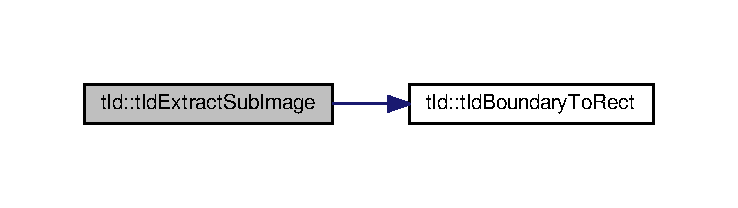
\includegraphics[width=350pt]{namespacetld_a16fe2b016494fa66be611f723ed7bebc_cgraph}
\end{center}
\end{figure}




Here is the caller graph for this function\-:\nopagebreak
\begin{figure}[H]
\begin{center}
\leavevmode
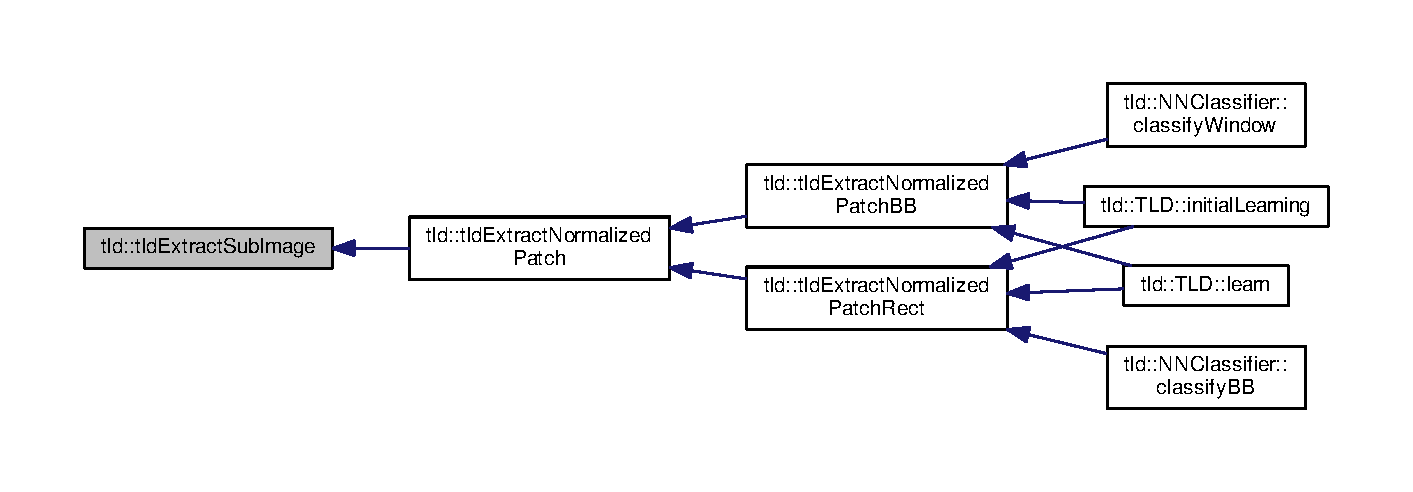
\includegraphics[width=350pt]{namespacetld_a16fe2b016494fa66be611f723ed7bebc_icgraph}
\end{center}
\end{figure}


\hypertarget{namespacetld_a7699b7dc20502fc6d7c5c6c6cbd4be7b}{\index{tld@{tld}!tld\-Extract\-Sub\-Image@{tld\-Extract\-Sub\-Image}}
\index{tld\-Extract\-Sub\-Image@{tld\-Extract\-Sub\-Image}!tld@{tld}}
\subsubsection[{tld\-Extract\-Sub\-Image}]{\setlength{\rightskip}{0pt plus 5cm}void tld\-::tld\-Extract\-Sub\-Image (
\begin{DoxyParamCaption}
\item[{const cv\-::\-Mat \&}]{img, }
\item[{cv\-::\-Mat \&}]{sub\-Image, }
\item[{int}]{x, }
\item[{int}]{y, }
\item[{int}]{w, }
\item[{int}]{h}
\end{DoxyParamCaption}
)}}\label{namespacetld_a7699b7dc20502fc6d7c5c6c6cbd4be7b}


Extracts the subimage by the reactangle. 


\begin{DoxyParams}{Parameters}
{\em img} & the source image \\
\hline
{\em sub\-Image} & the destination subimage \\
\hline
{\em x} & the x coordinate of the left top point of reactangle \\
\hline
{\em y} & the y coordinate of the left top point of reactangle \\
\hline
{\em w} & the width reactangle \\
\hline
{\em h} & the height reactangle \\
\hline
\end{DoxyParams}
\hypertarget{namespacetld_a8b28e6d4868ad30e826a6248dd2ae7a0}{\index{tld@{tld}!tld\-Is\-Inside@{tld\-Is\-Inside}}
\index{tld\-Is\-Inside@{tld\-Is\-Inside}!tld@{tld}}
\subsubsection[{tld\-Is\-Inside}]{\setlength{\rightskip}{0pt plus 5cm}int tld\-::tld\-Is\-Inside (
\begin{DoxyParamCaption}
\item[{int $\ast$}]{bb1, }
\item[{int $\ast$}]{bb2}
\end{DoxyParamCaption}
)}}\label{namespacetld_a8b28e6d4868ad30e826a6248dd2ae7a0}


Checks whether the one bouning box is completely inside the other. 


\begin{DoxyParams}{Parameters}
{\em bb1} & the one bouning box \\
\hline
{\em bb2} & the other bouning box \\
\hline
\end{DoxyParams}
\begin{DoxyReturn}{Returns}
1, if the one bouning box is completely inside the other; 0, otherwise 
\end{DoxyReturn}


Here is the caller graph for this function\-:\nopagebreak
\begin{figure}[H]
\begin{center}
\leavevmode
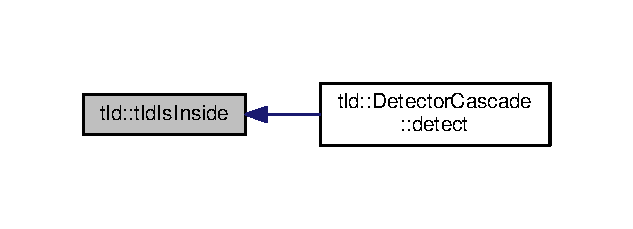
\includegraphics[width=304pt]{namespacetld_a8b28e6d4868ad30e826a6248dd2ae7a0_icgraph}
\end{center}
\end{figure}


\hypertarget{namespacetld_a7facbe495da1f0e058c78b9b7dea412a}{\index{tld@{tld}!tld\-Normalize\-Img@{tld\-Normalize\-Img}}
\index{tld\-Normalize\-Img@{tld\-Normalize\-Img}!tld@{tld}}
\subsubsection[{tld\-Normalize\-Img}]{\setlength{\rightskip}{0pt plus 5cm}void tld\-::tld\-Normalize\-Img (
\begin{DoxyParamCaption}
\item[{const cv\-::\-Mat \&}]{img, }
\item[{float $\ast$}]{output}
\end{DoxyParamCaption}
)}}\label{namespacetld_a7facbe495da1f0e058c78b9b7dea412a}


Returns mean-\/normalized patch, the image must be greyscale. 


\begin{DoxyParams}{Parameters}
{\em img} & the source image \\
\hline
{\em output} & the destination array (patch) \\
\hline
\end{DoxyParams}


Here is the caller graph for this function\-:\nopagebreak
\begin{figure}[H]
\begin{center}
\leavevmode
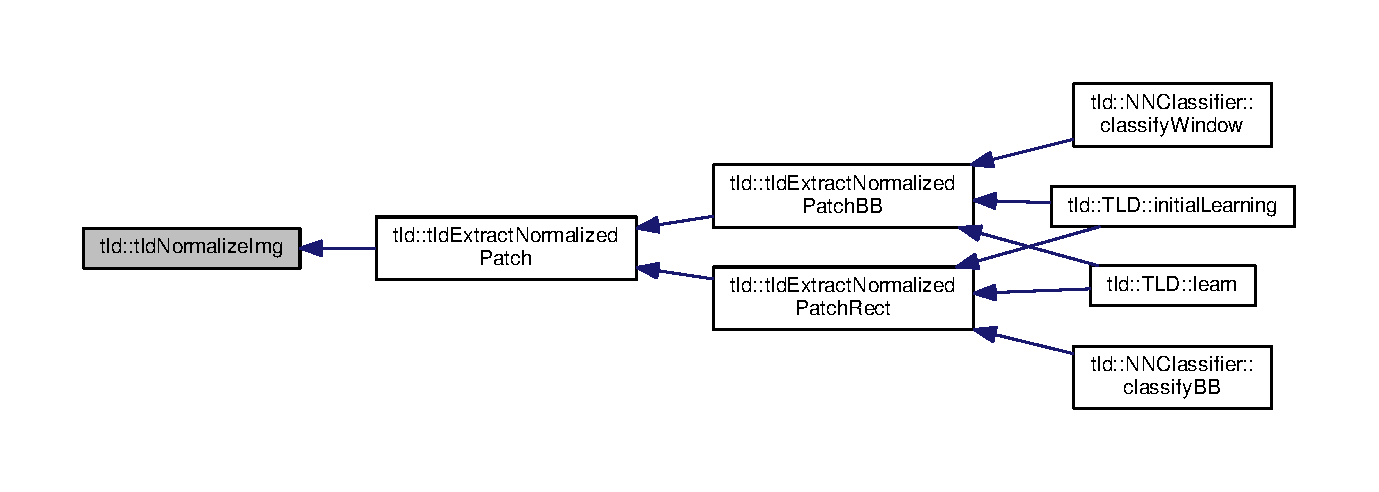
\includegraphics[width=350pt]{namespacetld_a7facbe495da1f0e058c78b9b7dea412a_icgraph}
\end{center}
\end{figure}


\hypertarget{namespacetld_aa9470de30170cb8b3f877dcae45df1b1}{\index{tld@{tld}!tld\-Overlap@{tld\-Overlap}}
\index{tld\-Overlap@{tld\-Overlap}!tld@{tld}}
\subsubsection[{tld\-Overlap}]{\setlength{\rightskip}{0pt plus 5cm}void tld\-::tld\-Overlap (
\begin{DoxyParamCaption}
\item[{int $\ast$}]{windows, }
\item[{int}]{num\-Windows, }
\item[{int $\ast$}]{boundary, }
\item[{float $\ast$}]{overlap}
\end{DoxyParamCaption}
)}}\label{namespacetld_aa9470de30170cb8b3f877dcae45df1b1}


Calculates the share overlap of windows and the boundary. 


\begin{DoxyParams}{Parameters}
{\em windows} & the array of windows \\
\hline
{\em num\-Windows} & the number of windows \\
\hline
{\em boundary} & the array (size 4) \\
\hline
{\em overlap} & the destination array \\
\hline
\end{DoxyParams}


Here is the call graph for this function\-:\nopagebreak
\begin{figure}[H]
\begin{center}
\leavevmode
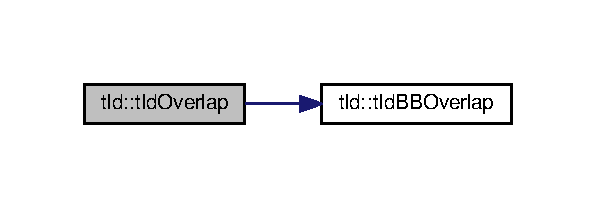
\includegraphics[width=286pt]{namespacetld_aa9470de30170cb8b3f877dcae45df1b1_cgraph}
\end{center}
\end{figure}




Here is the caller graph for this function\-:\nopagebreak
\begin{figure}[H]
\begin{center}
\leavevmode
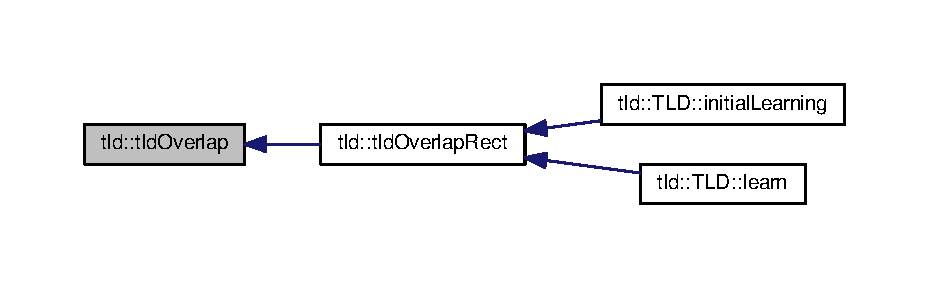
\includegraphics[width=350pt]{namespacetld_aa9470de30170cb8b3f877dcae45df1b1_icgraph}
\end{center}
\end{figure}


\hypertarget{namespacetld_a018caa7bf4a554814fe61a679a219489}{\index{tld@{tld}!tld\-Overlap\-One@{tld\-Overlap\-One}}
\index{tld\-Overlap\-One@{tld\-Overlap\-One}!tld@{tld}}
\subsubsection[{tld\-Overlap\-One}]{\setlength{\rightskip}{0pt plus 5cm}void tld\-::tld\-Overlap\-One (
\begin{DoxyParamCaption}
\item[{int $\ast$}]{windows, }
\item[{int}]{num\-Windows, }
\item[{int}]{index, }
\item[{std\-::vector$<$ int $>$ $\ast$}]{indices, }
\item[{float $\ast$}]{overlap}
\end{DoxyParamCaption}
)}}\label{namespacetld_a018caa7bf4a554814fe61a679a219489}


Calculates the share overlap of one window and the indexed windows (according). 


\begin{DoxyParams}{Parameters}
{\em windows} & the array of windows \\
\hline
{\em num\-Windows} & the number of windows \\
\hline
{\em index} & the index of one window \\
\hline
{\em indices} & the array of the indices of windows \\
\hline
{\em overlap} & the destination array \\
\hline
\end{DoxyParams}


Here is the call graph for this function\-:\nopagebreak
\begin{figure}[H]
\begin{center}
\leavevmode
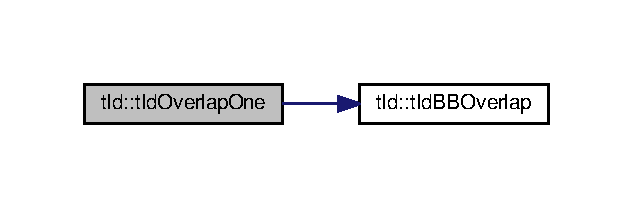
\includegraphics[width=304pt]{namespacetld_a018caa7bf4a554814fe61a679a219489_cgraph}
\end{center}
\end{figure}




Here is the caller graph for this function\-:\nopagebreak
\begin{figure}[H]
\begin{center}
\leavevmode
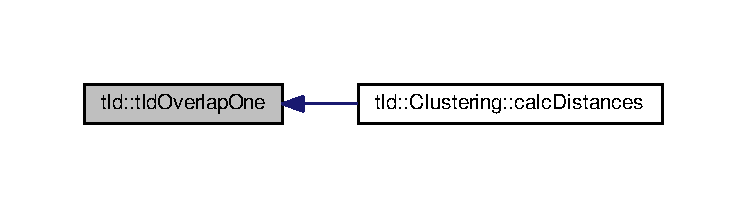
\includegraphics[width=350pt]{namespacetld_a018caa7bf4a554814fe61a679a219489_icgraph}
\end{center}
\end{figure}


\hypertarget{namespacetld_ae87c7dbe6b4da1e1923c42bec18caaf6}{\index{tld@{tld}!tld\-Overlap\-Rect@{tld\-Overlap\-Rect}}
\index{tld\-Overlap\-Rect@{tld\-Overlap\-Rect}!tld@{tld}}
\subsubsection[{tld\-Overlap\-Rect}]{\setlength{\rightskip}{0pt plus 5cm}void tld\-::tld\-Overlap\-Rect (
\begin{DoxyParamCaption}
\item[{int $\ast$}]{windows, }
\item[{int}]{num\-Windows, }
\item[{cv\-::\-Rect $\ast$}]{boundary, }
\item[{float $\ast$}]{overlap}
\end{DoxyParamCaption}
)}}\label{namespacetld_ae87c7dbe6b4da1e1923c42bec18caaf6}


Calculates the share overlap of windows and the rectangle. 


\begin{DoxyParams}{Parameters}
{\em windows} & the array of windows \\
\hline
{\em num\-Windows} & the number of windows \\
\hline
{\em boundary} & the rectangle \\
\hline
{\em overlap} & the destination array \\
\hline
\end{DoxyParams}


Here is the call graph for this function\-:\nopagebreak
\begin{figure}[H]
\begin{center}
\leavevmode
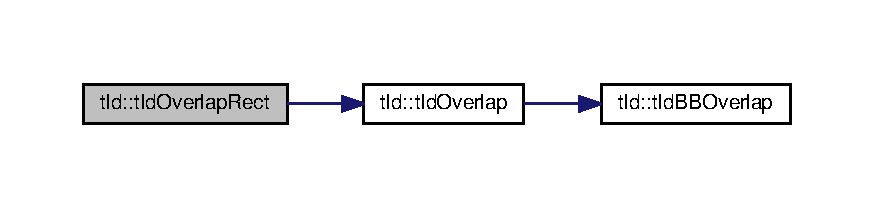
\includegraphics[width=350pt]{namespacetld_ae87c7dbe6b4da1e1923c42bec18caaf6_cgraph}
\end{center}
\end{figure}




Here is the caller graph for this function\-:\nopagebreak
\begin{figure}[H]
\begin{center}
\leavevmode
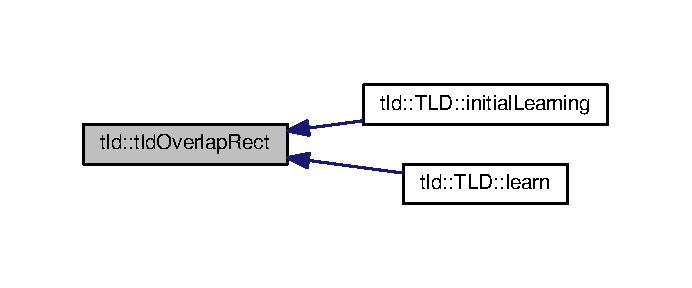
\includegraphics[width=332pt]{namespacetld_ae87c7dbe6b4da1e1923c42bec18caaf6_icgraph}
\end{center}
\end{figure}


\hypertarget{namespacetld_afdab54607fed863cdc408f72fd0f774b}{\index{tld@{tld}!tld\-Overlap\-Rect\-Rect@{tld\-Overlap\-Rect\-Rect}}
\index{tld\-Overlap\-Rect\-Rect@{tld\-Overlap\-Rect\-Rect}!tld@{tld}}
\subsubsection[{tld\-Overlap\-Rect\-Rect}]{\setlength{\rightskip}{0pt plus 5cm}float tld\-::tld\-Overlap\-Rect\-Rect (
\begin{DoxyParamCaption}
\item[{cv\-::\-Rect}]{r1, }
\item[{cv\-::\-Rect}]{r2}
\end{DoxyParamCaption}
)}}\label{namespacetld_afdab54607fed863cdc408f72fd0f774b}


Calculates the share overlap of two rectangle (the share the intersection area in the occupy area). 


\begin{DoxyParams}{Parameters}
{\em r1} & the one rectangle \\
\hline
{\em r2} & the two rectangle \\
\hline
\end{DoxyParams}
\begin{DoxyReturn}{Returns}
the share overlap(0 to 1) 
\end{DoxyReturn}


Here is the call graph for this function\-:\nopagebreak
\begin{figure}[H]
\begin{center}
\leavevmode
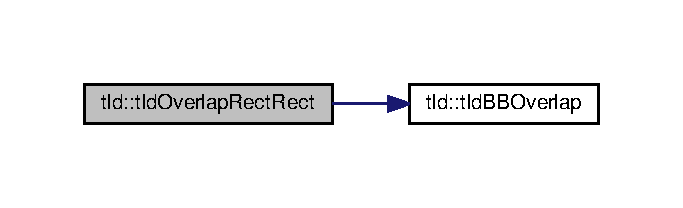
\includegraphics[width=328pt]{namespacetld_afdab54607fed863cdc408f72fd0f774b_cgraph}
\end{center}
\end{figure}




Here is the caller graph for this function\-:\nopagebreak
\begin{figure}[H]
\begin{center}
\leavevmode
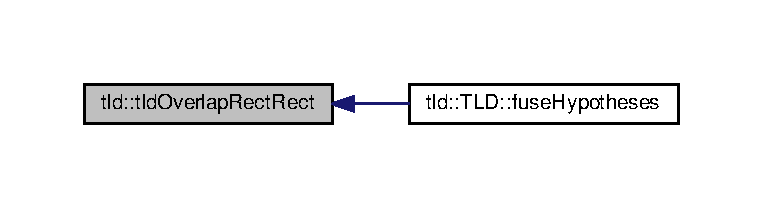
\includegraphics[width=350pt]{namespacetld_afdab54607fed863cdc408f72fd0f774b_icgraph}
\end{center}
\end{figure}


\hypertarget{namespacetld_a18975268ebbf3daf5eaf46d30fd782e9}{\index{tld@{tld}!tld\-Rect\-To\-Array@{tld\-Rect\-To\-Array}}
\index{tld\-Rect\-To\-Array@{tld\-Rect\-To\-Array}!tld@{tld}}
\subsubsection[{tld\-Rect\-To\-Array}]{\setlength{\rightskip}{0pt plus 5cm}template$<$class T $>$ void tld\-::tld\-Rect\-To\-Array (
\begin{DoxyParamCaption}
\item[{cv\-::\-Rect}]{rect, }
\item[{T $\ast$}]{boundary}
\end{DoxyParamCaption}
)}}\label{namespacetld_a18975268ebbf3daf5eaf46d30fd782e9}


Converts the rectangle to array (size 4). 


\begin{DoxyParams}{Parameters}
{\em rect} & the source rectangle \\
\hline
{\em boundary} & the destination array \\
\hline
\end{DoxyParams}


Here is the caller graph for this function\-:\nopagebreak
\begin{figure}[H]
\begin{center}
\leavevmode
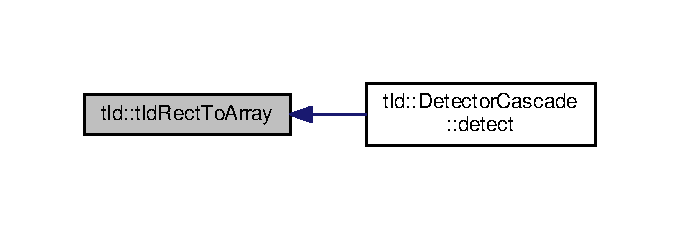
\includegraphics[width=326pt]{namespacetld_a18975268ebbf3daf5eaf46d30fd782e9_icgraph}
\end{center}
\end{figure}


\hypertarget{namespacetld_ac0c16951370c978dee562ac3d3bd1554}{\index{tld@{tld}!tld\-Rect\-To\-Points@{tld\-Rect\-To\-Points}}
\index{tld\-Rect\-To\-Points@{tld\-Rect\-To\-Points}!tld@{tld}}
\subsubsection[{tld\-Rect\-To\-Points}]{\setlength{\rightskip}{0pt plus 5cm}void tld\-::tld\-Rect\-To\-Points (
\begin{DoxyParamCaption}
\item[{Cv\-Rect}]{rect, }
\item[{Cv\-Point $\ast$}]{p1, }
\item[{Cv\-Point $\ast$}]{p2}
\end{DoxyParamCaption}
)}}\label{namespacetld_ac0c16951370c978dee562ac3d3bd1554}


Converts the rectangle to two points. 


\begin{DoxyParams}{Parameters}
{\em rect} & the rectangle \\
\hline
{\em p1} & the left top point \\
\hline
{\em p2} & the right bottom point \\
\hline
\end{DoxyParams}
\hypertarget{namespacetld_acaf374df081816ecaf9079e200a8f5af}{\index{tld@{tld}!tld\-Sort\-By\-Overlap\-Desc@{tld\-Sort\-By\-Overlap\-Desc}}
\index{tld\-Sort\-By\-Overlap\-Desc@{tld\-Sort\-By\-Overlap\-Desc}!tld@{tld}}
\subsubsection[{tld\-Sort\-By\-Overlap\-Desc}]{\setlength{\rightskip}{0pt plus 5cm}bool tld\-::tld\-Sort\-By\-Overlap\-Desc (
\begin{DoxyParamCaption}
\item[{std\-::pair$<$ int, float $>$}]{bb1, }
\item[{std\-::pair$<$ int, float $>$}]{bb2}
\end{DoxyParamCaption}
)}}\label{namespacetld_acaf374df081816ecaf9079e200a8f5af}


Checks whether the second parameter of one pair is more then the second parameter of other pair. 


\begin{DoxyParams}{Parameters}
{\em bb1} & the one pair \\
\hline
{\em bb2} & the other pair \\
\hline
\end{DoxyParams}
\begin{DoxyReturn}{Returns}
the result of comparing 
\end{DoxyReturn}


Here is the caller graph for this function\-:\nopagebreak
\begin{figure}[H]
\begin{center}
\leavevmode
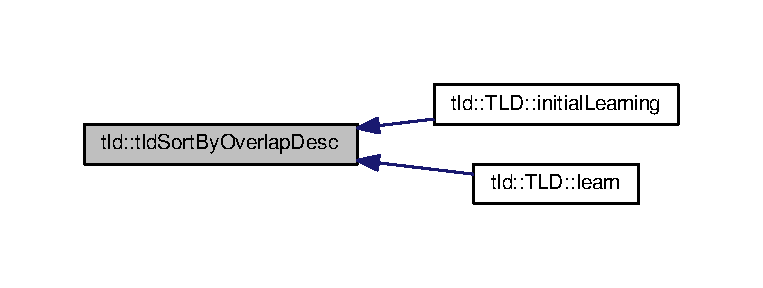
\includegraphics[width=350pt]{namespacetld_acaf374df081816ecaf9079e200a8f5af_icgraph}
\end{center}
\end{figure}




\subsection{Variable Documentation}
\hypertarget{namespacetld_aa5e13bbb9a53d3e9103d430b6113b08b}{\index{tld@{tld}!bb@{bb}}
\index{bb@{bb}!tld@{tld}}
\subsubsection[{bb}]{\setlength{\rightskip}{0pt plus 5cm}Cv\-Rect$\ast$ tld\-::bb\hspace{0.3cm}{\ttfamily [static]}}}\label{namespacetld_aa5e13bbb9a53d3e9103d430b6113b08b}
\hypertarget{namespacetld_a7cfa165f34457693b8898cfa78e51945}{\index{tld@{tld}!drag@{drag}}
\index{drag@{drag}!tld@{tld}}
\subsubsection[{drag}]{\setlength{\rightskip}{0pt plus 5cm}int tld\-::drag = 0\hspace{0.3cm}{\ttfamily [static]}}}\label{namespacetld_a7cfa165f34457693b8898cfa78e51945}
\hypertarget{namespacetld_a16a44df30fb791b45dd103ba1541fb67}{\index{tld@{tld}!font@{font}}
\index{font@{font}!tld@{tld}}
\subsubsection[{font}]{\setlength{\rightskip}{0pt plus 5cm}Cv\-Font tld\-::font\hspace{0.3cm}{\ttfamily [static]}}}\label{namespacetld_a16a44df30fb791b45dd103ba1541fb67}
\hypertarget{namespacetld_a17f0b1eb181c0395a541e031b203040a}{\index{tld@{tld}!help\-\_\-text@{help\-\_\-text}}
\index{help\-\_\-text@{help\-\_\-text}!tld@{tld}}
\subsubsection[{help\-\_\-text}]{\setlength{\rightskip}{0pt plus 5cm}char tld\-::help\-\_\-text\mbox{[}$\,$\mbox{]}\hspace{0.3cm}{\ttfamily [static]}}}\label{namespacetld_a17f0b1eb181c0395a541e031b203040a}
{\bfseries Initial value\-:}
\begin{DoxyCode}
=
    \textcolor{stringliteral}{"usage: tld [option arguments] [arguments]\(\backslash\)n"}
    \textcolor{stringliteral}{"option arguments:\(\backslash\)n"}
    \textcolor{stringliteral}{"[-a <startFrameNumber>] video starts at the frameNumber <startFrameNumber>\(\backslash\)n"}
    \textcolor{stringliteral}{"[-b <x,y,w,h>] Initial bounding box\(\backslash\)n"}
    \textcolor{stringliteral}{"[-c] shows color images instead of greyscale\(\backslash\)n"}
    \textcolor{stringliteral}{"[-d <device>] select input device: <device>=(IMGS|CAM|VID)\(\backslash\)n"}
    \textcolor{stringliteral}{"    IMGS: capture from images\(\backslash\)n"}
    \textcolor{stringliteral}{"    CAM: capture from connected camera\(\backslash\)n"}
    \textcolor{stringliteral}{"    VID: capture from a video\(\backslash\)n"}
    \textcolor{stringliteral}{"    STREAM: capture from a stream\(\backslash\)n"}
    \textcolor{stringliteral}{"[-e <path>] export model after run to <path>\(\backslash\)n"}
    \textcolor{stringliteral}{"[-f] shows foreground\(\backslash\)n"}
    \textcolor{stringliteral}{"[-i <path>] <path> to the images or to the video\(\backslash\)n"}
    \textcolor{stringliteral}{"[-h] shows help\(\backslash\)n"}
    \textcolor{stringliteral}{"[-j <number>] specifies the <number> of the last frames which are considered by the trajectory; 0
       disables the trajectory\(\backslash\)n"}
    \textcolor{stringliteral}{"[-m <path>] if specified load a model from <path>. An initialBoundingBox must be specified or
       selectManually must be true.\(\backslash\)n"}
    \textcolor{stringliteral}{"[-n <number>] specifies which camera device to use.\(\backslash\)n"}
    \textcolor{stringliteral}{"[-p <path>] prints results into the file <path>\(\backslash\)n"}
    \textcolor{stringliteral}{"[-s] if set, user can select initial bounding box\(\backslash\)n"}
    \textcolor{stringliteral}{"[-t <theta>] threshold for determining positive results\(\backslash\)n"}
    \textcolor{stringliteral}{"[-z <lastFrameNumber>] video ends at the frameNumber <lastFrameNumber>.\(\backslash\)n"}
    \textcolor{stringliteral}{"    If <lastFrameNumber> is 0 or the option argument isn't specified means\(\backslash\)n"}
    \textcolor{stringliteral}{"    take all frames.\(\backslash\)n"}
    \textcolor{stringliteral}{"arguments:\(\backslash\)n"}
    \textcolor{stringliteral}{"[<path>] <path> to the config file\(\backslash\)n"}
\end{DoxyCode}
\hypertarget{namespacetld_a32bc4295eda098201cd336e2d2f1e217}{\index{tld@{tld}!img0@{img0}}
\index{img0@{img0}!tld@{tld}}
\subsubsection[{img0}]{\setlength{\rightskip}{0pt plus 5cm}Ipl\-Image$\ast$ tld\-::img0\hspace{0.3cm}{\ttfamily [static]}}}\label{namespacetld_a32bc4295eda098201cd336e2d2f1e217}
\hypertarget{namespacetld_ac832a3e8122e594c1c5321935cbc2639}{\index{tld@{tld}!img1@{img1}}
\index{img1@{img1}!tld@{tld}}
\subsubsection[{img1}]{\setlength{\rightskip}{0pt plus 5cm}Ipl\-Image$\ast$ tld\-::img1\hspace{0.3cm}{\ttfamily [static]}}}\label{namespacetld_ac832a3e8122e594c1c5321935cbc2639}
\hypertarget{namespacetld_a1bbc7d3201a2ef41da5495e0e48cfd2e}{\index{tld@{tld}!optarg@{optarg}}
\index{optarg@{optarg}!tld@{tld}}
\subsubsection[{optarg}]{\setlength{\rightskip}{0pt plus 5cm}char $\ast$ tld\-::optarg}}\label{namespacetld_a1bbc7d3201a2ef41da5495e0e48cfd2e}
\hypertarget{namespacetld_a6e180d5067af278cc277ae9c6f7507c1}{\index{tld@{tld}!opterr@{opterr}}
\index{opterr@{opterr}!tld@{tld}}
\subsubsection[{opterr}]{\setlength{\rightskip}{0pt plus 5cm}int tld\-::opterr = 1}}\label{namespacetld_a6e180d5067af278cc277ae9c6f7507c1}
\hypertarget{namespacetld_ab8c5a378ef03678c537edc84a15abc22}{\index{tld@{tld}!optind@{optind}}
\index{optind@{optind}!tld@{tld}}
\subsubsection[{optind}]{\setlength{\rightskip}{0pt plus 5cm}int tld\-::optind = 1}}\label{namespacetld_ab8c5a378ef03678c537edc84a15abc22}
\hypertarget{namespacetld_a6d6bd80732b9f396bc03e5f2c5cf30f8}{\index{tld@{tld}!optopt@{optopt}}
\index{optopt@{optopt}!tld@{tld}}
\subsubsection[{optopt}]{\setlength{\rightskip}{0pt plus 5cm}int tld\-::optopt}}\label{namespacetld_a6d6bd80732b9f396bc03e5f2c5cf30f8}
\hypertarget{namespacetld_a680868c3e5a47352c5353897519636d4}{\index{tld@{tld}!point@{point}}
\index{point@{point}!tld@{tld}}
\subsubsection[{point}]{\setlength{\rightskip}{0pt plus 5cm}Cv\-Point tld\-::point\hspace{0.3cm}{\ttfamily [static]}}}\label{namespacetld_a680868c3e5a47352c5353897519636d4}
\hypertarget{namespacetld_a7a647c1eaeda30086f4519b611db4e71}{\index{tld@{tld}!T\-L\-D\-\_\-\-W\-I\-N\-D\-O\-W\-\_\-\-O\-F\-F\-S\-E\-T\-\_\-\-S\-I\-Z\-E@{T\-L\-D\-\_\-\-W\-I\-N\-D\-O\-W\-\_\-\-O\-F\-F\-S\-E\-T\-\_\-\-S\-I\-Z\-E}}
\index{T\-L\-D\-\_\-\-W\-I\-N\-D\-O\-W\-\_\-\-O\-F\-F\-S\-E\-T\-\_\-\-S\-I\-Z\-E@{T\-L\-D\-\_\-\-W\-I\-N\-D\-O\-W\-\_\-\-O\-F\-F\-S\-E\-T\-\_\-\-S\-I\-Z\-E}!tld@{tld}}
\subsubsection[{T\-L\-D\-\_\-\-W\-I\-N\-D\-O\-W\-\_\-\-O\-F\-F\-S\-E\-T\-\_\-\-S\-I\-Z\-E}]{\setlength{\rightskip}{0pt plus 5cm}const int tld\-::\-T\-L\-D\-\_\-\-W\-I\-N\-D\-O\-W\-\_\-\-O\-F\-F\-S\-E\-T\-\_\-\-S\-I\-Z\-E = 6\hspace{0.3cm}{\ttfamily [static]}}}\label{namespacetld_a7a647c1eaeda30086f4519b611db4e71}


the size of array, defining the window offset 

\hypertarget{namespacetld_ad0458a97a7973a088840e7917515c6ae}{\index{tld@{tld}!T\-L\-D\-\_\-\-W\-I\-N\-D\-O\-W\-\_\-\-S\-I\-Z\-E@{T\-L\-D\-\_\-\-W\-I\-N\-D\-O\-W\-\_\-\-S\-I\-Z\-E}}
\index{T\-L\-D\-\_\-\-W\-I\-N\-D\-O\-W\-\_\-\-S\-I\-Z\-E@{T\-L\-D\-\_\-\-W\-I\-N\-D\-O\-W\-\_\-\-S\-I\-Z\-E}!tld@{tld}}
\subsubsection[{T\-L\-D\-\_\-\-W\-I\-N\-D\-O\-W\-\_\-\-S\-I\-Z\-E}]{\setlength{\rightskip}{0pt plus 5cm}const int tld\-::\-T\-L\-D\-\_\-\-W\-I\-N\-D\-O\-W\-\_\-\-S\-I\-Z\-E = 5\hspace{0.3cm}{\ttfamily [static]}}}\label{namespacetld_ad0458a97a7973a088840e7917515c6ae}


the size of array, defining the window 

\hypertarget{namespacetld_ad1bfc03770cc333da8a972ab7d35c246}{\index{tld@{tld}!window\-\_\-name@{window\-\_\-name}}
\index{window\-\_\-name@{window\-\_\-name}!tld@{tld}}
\subsubsection[{window\-\_\-name}]{\setlength{\rightskip}{0pt plus 5cm}string tld\-::window\-\_\-name\hspace{0.3cm}{\ttfamily [static]}}}\label{namespacetld_ad1bfc03770cc333da8a972ab7d35c246}

\chapter{Class Documentation}
\hypertarget{classCBlob}{\section{C\-Blob Class Reference}
\label{classCBlob}\index{C\-Blob@{C\-Blob}}
}


Blob class.  




{\ttfamily \#include $<$blob.\-h$>$}



Collaboration diagram for C\-Blob\-:\nopagebreak
\begin{figure}[H]
\begin{center}
\leavevmode
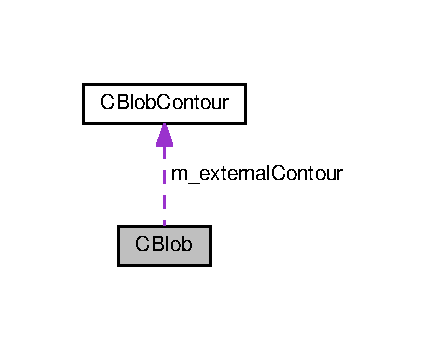
\includegraphics[width=205pt]{classCBlob__coll__graph}
\end{center}
\end{figure}
\subsection*{Public Member Functions}
\begin{DoxyCompactItemize}
\item 
\hyperlink{classCBlob_acd24304c1bc98128b24914f3e4bfea7c}{C\-Blob} ()
\item 
\hyperlink{classCBlob_a45d7bbe67ef246fe180e16f5a7116c6f}{C\-Blob} (\hyperlink{blob_8h_ae21ba61a4f023a2f91fc5feaad495073}{t\-\_\-label\-Type} id, Cv\-Point start\-Point, Cv\-Size original\-Image\-Size)
\item 
\hyperlink{classCBlob_a593ffb9ba17290432d04c383f2f104e2}{$\sim$\-C\-Blob} ()
\item 
\hyperlink{classCBlob_af87156ca1ac7f64a860b7cf8c07fd1fa}{C\-Blob} (const \hyperlink{classCBlob}{C\-Blob} \&src)
\begin{DoxyCompactList}\small\item\em Copy constructor. \end{DoxyCompactList}\item 
\hyperlink{classCBlob_a61719b6e5ebff6d3e383b98bce4137dc}{C\-Blob} (const \hyperlink{classCBlob}{C\-Blob} $\ast$src)
\item 
\hyperlink{classCBlob}{C\-Blob} \& \hyperlink{classCBlob_a724e55442a030bf94da856310e324a40}{operator=} (const \hyperlink{classCBlob}{C\-Blob} \&src)
\item 
void \hyperlink{classCBlob_ad26a1bc4e31809c3bd76424b05824e90}{Add\-Internal\-Contour} (const \hyperlink{classCBlobContour}{C\-Blob\-Contour} \&new\-Contour)
\begin{DoxyCompactList}\small\item\em Adds a new internal contour to the blob. \end{DoxyCompactList}\item 
\hyperlink{classCBlobContour}{C\-Blob\-Contour} $\ast$ \hyperlink{classCBlob_ad136387165bd74c368cb4ecc7632e4cf}{Get\-External\-Contour} ()
\begin{DoxyCompactList}\small\item\em Retrieves contour in Freeman's chain code. \end{DoxyCompactList}\item 
Cv\-Mem\-Storage $\ast$ \hyperlink{classCBlob_a1eeee72a4369dc9485c6ae6573631a02}{Get\-Storage} ()
\begin{DoxyCompactList}\small\item\em Retrieves blob storage. \end{DoxyCompactList}\item 
\hyperlink{blob_8h_ae21ba61a4f023a2f91fc5feaad495073}{t\-\_\-label\-Type} \hyperlink{classCBlob_a1d3fd90bc98f6d845babb18a3f058bc2}{Get\-I\-D} ()
\begin{DoxyCompactList}\small\item\em Get label I\-D. \end{DoxyCompactList}\item 
int \hyperlink{classCBlob_a2d56a7dee1cbeb3178ff083630ee31b0}{Exterior} (Ipl\-Image $\ast$mask, bool x\-Border=true, bool y\-Border=true)
\begin{DoxyCompactList}\small\item\em \begin{quotation}
0 for extern blobs, 0 if not \end{quotation}
\end{DoxyCompactList}\item 
double \hyperlink{classCBlob_a6f1db9fcb42c0a3ea003aaeb0ec65a8d}{Area} ()
\begin{DoxyCompactList}\small\item\em Compute blob's area. \end{DoxyCompactList}\item 
double \hyperlink{classCBlob_af63853ea55dbebbee5b013189e765b51}{Perimeter} ()
\begin{DoxyCompactList}\small\item\em Compute blob's perimeter. \end{DoxyCompactList}\item 
double \hyperlink{classCBlob_a4f5dfca1ee933e07a39965375f9f07c5}{Moment} (int p, int q)
\begin{DoxyCompactList}\small\item\em Compute blob's moment (p,q up to M\-A\-X\-\_\-\-C\-A\-L\-C\-U\-L\-A\-T\-E\-D\-\_\-\-M\-O\-M\-E\-N\-T\-S) \end{DoxyCompactList}\item 
double \hyperlink{classCBlob_ab1501b07a2c5ee23843bac66d20974e2}{Extern\-Perimeter} (Ipl\-Image $\ast$mask, bool x\-Border=true, bool y\-Border=true)
\begin{DoxyCompactList}\small\item\em Compute extern perimeter. \end{DoxyCompactList}\item 
double \hyperlink{classCBlob_a1b12d25f8e470fdd808ac2e3bfe9bad4}{Mean} (Ipl\-Image $\ast$image)
\begin{DoxyCompactList}\small\item\em Get mean grey color. \end{DoxyCompactList}\item 
double \hyperlink{classCBlob_a014b670bb748e6767ef070e1bc25be7a}{Std\-Dev} (Ipl\-Image $\ast$image)
\begin{DoxyCompactList}\small\item\em Get standard deviation grey color. \end{DoxyCompactList}\item 
bool \hyperlink{classCBlob_ac97e73d3040530de09a187d02632deb1}{Is\-Empty} ()
\item 
\hyperlink{BlobContour_8h_abf72b29b2c653dd623e9b39a447809c0}{t\-\_\-\-Point\-List} \hyperlink{classCBlob_aacc50d5d47e0543d4e0a569d05009006}{Get\-Convex\-Hull} ()
\item 
void \hyperlink{classCBlob_a1a12b6dee61d2db86cd3a60c0671382e}{Fill\-Blob} (Ipl\-Image $\ast$imatge, Cv\-Scalar color, int offset\-X=0, int offset\-Y=0)
\item 
void \hyperlink{classCBlob_a006463cc42ef0e4b8986fa5020cb6f90}{Join\-Blob} (\hyperlink{classCBlob}{C\-Blob} $\ast$blob)
\begin{DoxyCompactList}\small\item\em Join a blob to current one (add's contour. \end{DoxyCompactList}\item 
Cv\-Rect \hyperlink{classCBlob_a5391167c172eb461eb762fbdd81306de}{Get\-Bounding\-Box} ()
\begin{DoxyCompactList}\small\item\em Get bounding box. \end{DoxyCompactList}\item 
Cv\-Box2\-D \hyperlink{classCBlob_ad0bb95f395084ee89ca35cf11f203342}{Get\-Ellipse} ()
\begin{DoxyCompactList}\small\item\em Get bounding ellipse. \end{DoxyCompactList}\item 
double \hyperlink{classCBlob_aa3313af22e7f28d65ba245bc3b8a30bc}{Min\-X} ()
\begin{DoxyCompactList}\small\item\em Minimun X. \end{DoxyCompactList}\item 
double \hyperlink{classCBlob_a44e2caf6c7fc6e8360d2576c18c9bc2b}{Min\-Y} ()
\begin{DoxyCompactList}\small\item\em Minimun Y. \end{DoxyCompactList}\item 
double \hyperlink{classCBlob_ab26a757fffc581df39620425de008cbc}{Max\-X} ()
\begin{DoxyCompactList}\small\item\em Maximun X. \end{DoxyCompactList}\item 
double \hyperlink{classCBlob_a740a37afcd841bf719587d2f0128c555}{Max\-Y} ()
\begin{DoxyCompactList}\small\item\em Maximun Y. \end{DoxyCompactList}\end{DoxyCompactItemize}
\subsection*{Private Types}
\begin{DoxyCompactItemize}
\item 
typedef std\-::list$<$ \hyperlink{classCBlobContour}{C\-Blob\-Contour} $>$ \hyperlink{classCBlob_a6c917467ff363aa242e6a46cde41da79}{t\-\_\-contour\-List}
\end{DoxyCompactItemize}
\subsection*{Private Member Functions}
\begin{DoxyCompactItemize}
\item 
void \hyperlink{classCBlob_a4e3c8e5c89036d0a141ca8f839e4e7e3}{Clear\-Contours} ()
\begin{DoxyCompactList}\small\item\em Deallocates all contours. \end{DoxyCompactList}\end{DoxyCompactItemize}
\subsection*{Private Attributes}
\begin{DoxyCompactItemize}
\item 
Cv\-Mem\-Storage $\ast$ \hyperlink{classCBlob_aca7cb0f750e553fa34935ea927fd2122}{m\-\_\-storage}
\begin{DoxyCompactList}\small\item\em Contour storage memory. \end{DoxyCompactList}\item 
\hyperlink{classCBlobContour}{C\-Blob\-Contour} \hyperlink{classCBlob_a6432d83f68a1c75464bb1c2f7450e4b5}{m\-\_\-external\-Contour}
\begin{DoxyCompactList}\small\item\em External contour of the blob (crack codes) \end{DoxyCompactList}\item 
\hyperlink{classCBlob_a6c917467ff363aa242e6a46cde41da79}{t\-\_\-contour\-List} \hyperlink{classCBlob_a88071948e0c48f4b256147df3a03a7de}{m\-\_\-internal\-Contours}
\begin{DoxyCompactList}\small\item\em Internal contours (crack codes) \end{DoxyCompactList}\item 
\hyperlink{blob_8h_ae21ba61a4f023a2f91fc5feaad495073}{t\-\_\-label\-Type} \hyperlink{classCBlob_aee7e60307972994de76d4128f08851c0}{m\-\_\-id}
\begin{DoxyCompactList}\small\item\em Label number. \end{DoxyCompactList}\item 
double \hyperlink{classCBlob_a9dd356b7cf492e6c8fa0109c81f6ac3c}{m\-\_\-area}
\begin{DoxyCompactList}\small\item\em Area. \end{DoxyCompactList}\item 
double \hyperlink{classCBlob_a4d08eee6c8bb843469afa60834707bb8}{m\-\_\-perimeter}
\begin{DoxyCompactList}\small\item\em Perimeter. \end{DoxyCompactList}\item 
double \hyperlink{classCBlob_adf1b82bc3602c5d08028730ee3a3d47e}{m\-\_\-extern\-Perimeter}
\begin{DoxyCompactList}\small\item\em Extern perimeter from blob. \end{DoxyCompactList}\item 
double \hyperlink{classCBlob_aeb1c6a7e54a529c9231a96cbe644c9d4}{m\-\_\-mean\-Gray}
\begin{DoxyCompactList}\small\item\em Mean gray color. \end{DoxyCompactList}\item 
double \hyperlink{classCBlob_ab54c421db7988eef96af434d2cf0b0da}{m\-\_\-std\-Dev\-Gray}
\begin{DoxyCompactList}\small\item\em Standard deviation from gray color blob distribution. \end{DoxyCompactList}\item 
Cv\-Rect \hyperlink{classCBlob_ad153da0682f927274e3493e0f0a8e9ff}{m\-\_\-bounding\-Box}
\begin{DoxyCompactList}\small\item\em Bounding box. \end{DoxyCompactList}\item 
Cv\-Box2\-D \hyperlink{classCBlob_aa06a47b96675de402b95dbbff330f3f0}{m\-\_\-ellipse}
\begin{DoxyCompactList}\small\item\em Bounding ellipse. \end{DoxyCompactList}\item 
Cv\-Size \hyperlink{classCBlob_a0dc76004877e49c4607ecf3bea800d49}{m\-\_\-original\-Image\-Size}
\begin{DoxyCompactList}\small\item\em Sizes from image where blob is extracted. \end{DoxyCompactList}\end{DoxyCompactItemize}


\subsection{Detailed Description}
Blob class. 

\subsection{Member Typedef Documentation}
\hypertarget{classCBlob_a6c917467ff363aa242e6a46cde41da79}{\index{C\-Blob@{C\-Blob}!t\-\_\-contour\-List@{t\-\_\-contour\-List}}
\index{t\-\_\-contour\-List@{t\-\_\-contour\-List}!CBlob@{C\-Blob}}
\subsubsection[{t\-\_\-contour\-List}]{\setlength{\rightskip}{0pt plus 5cm}typedef std\-::list$<${\bf C\-Blob\-Contour}$>$ {\bf C\-Blob\-::t\-\_\-contour\-List}\hspace{0.3cm}{\ttfamily [private]}}}\label{classCBlob_a6c917467ff363aa242e6a46cde41da79}


\subsection{Constructor \& Destructor Documentation}
\hypertarget{classCBlob_acd24304c1bc98128b24914f3e4bfea7c}{\index{C\-Blob@{C\-Blob}!C\-Blob@{C\-Blob}}
\index{C\-Blob@{C\-Blob}!CBlob@{C\-Blob}}
\subsubsection[{C\-Blob}]{\setlength{\rightskip}{0pt plus 5cm}C\-Blob\-::\-C\-Blob (
\begin{DoxyParamCaption}
{}
\end{DoxyParamCaption}
)}}\label{classCBlob_acd24304c1bc98128b24914f3e4bfea7c}
\hypertarget{classCBlob_a45d7bbe67ef246fe180e16f5a7116c6f}{\index{C\-Blob@{C\-Blob}!C\-Blob@{C\-Blob}}
\index{C\-Blob@{C\-Blob}!CBlob@{C\-Blob}}
\subsubsection[{C\-Blob}]{\setlength{\rightskip}{0pt plus 5cm}C\-Blob\-::\-C\-Blob (
\begin{DoxyParamCaption}
\item[{{\bf t\-\_\-label\-Type}}]{id, }
\item[{Cv\-Point}]{start\-Point, }
\item[{Cv\-Size}]{original\-Image\-Size}
\end{DoxyParamCaption}
)}}\label{classCBlob_a45d7bbe67ef246fe180e16f5a7116c6f}
\hypertarget{classCBlob_a593ffb9ba17290432d04c383f2f104e2}{\index{C\-Blob@{C\-Blob}!$\sim$\-C\-Blob@{$\sim$\-C\-Blob}}
\index{$\sim$\-C\-Blob@{$\sim$\-C\-Blob}!CBlob@{C\-Blob}}
\subsubsection[{$\sim$\-C\-Blob}]{\setlength{\rightskip}{0pt plus 5cm}C\-Blob\-::$\sim$\-C\-Blob (
\begin{DoxyParamCaption}
{}
\end{DoxyParamCaption}
)}}\label{classCBlob_a593ffb9ba17290432d04c383f2f104e2}


Here is the call graph for this function\-:\nopagebreak
\begin{figure}[H]
\begin{center}
\leavevmode
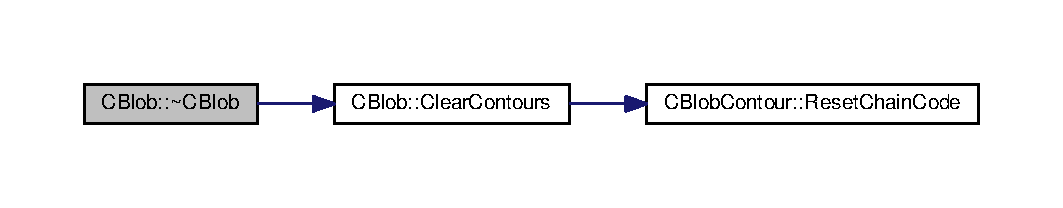
\includegraphics[width=350pt]{classCBlob_a593ffb9ba17290432d04c383f2f104e2_cgraph}
\end{center}
\end{figure}


\hypertarget{classCBlob_af87156ca1ac7f64a860b7cf8c07fd1fa}{\index{C\-Blob@{C\-Blob}!C\-Blob@{C\-Blob}}
\index{C\-Blob@{C\-Blob}!CBlob@{C\-Blob}}
\subsubsection[{C\-Blob}]{\setlength{\rightskip}{0pt plus 5cm}C\-Blob\-::\-C\-Blob (
\begin{DoxyParamCaption}
\item[{const {\bf C\-Blob} \&}]{src}
\end{DoxyParamCaption}
)}}\label{classCBlob_af87156ca1ac7f64a860b7cf8c07fd1fa}


Copy constructor. 

\hypertarget{classCBlob_a61719b6e5ebff6d3e383b98bce4137dc}{\index{C\-Blob@{C\-Blob}!C\-Blob@{C\-Blob}}
\index{C\-Blob@{C\-Blob}!CBlob@{C\-Blob}}
\subsubsection[{C\-Blob}]{\setlength{\rightskip}{0pt plus 5cm}C\-Blob\-::\-C\-Blob (
\begin{DoxyParamCaption}
\item[{const {\bf C\-Blob} $\ast$}]{src}
\end{DoxyParamCaption}
)}}\label{classCBlob_a61719b6e5ebff6d3e383b98bce4137dc}


\subsection{Member Function Documentation}
\hypertarget{classCBlob_ad26a1bc4e31809c3bd76424b05824e90}{\index{C\-Blob@{C\-Blob}!Add\-Internal\-Contour@{Add\-Internal\-Contour}}
\index{Add\-Internal\-Contour@{Add\-Internal\-Contour}!CBlob@{C\-Blob}}
\subsubsection[{Add\-Internal\-Contour}]{\setlength{\rightskip}{0pt plus 5cm}void C\-Blob\-::\-Add\-Internal\-Contour (
\begin{DoxyParamCaption}
\item[{const {\bf C\-Blob\-Contour} \&}]{new\-Contour}
\end{DoxyParamCaption}
)}}\label{classCBlob_ad26a1bc4e31809c3bd76424b05824e90}


Adds a new internal contour to the blob. 



Here is the caller graph for this function\-:\nopagebreak
\begin{figure}[H]
\begin{center}
\leavevmode
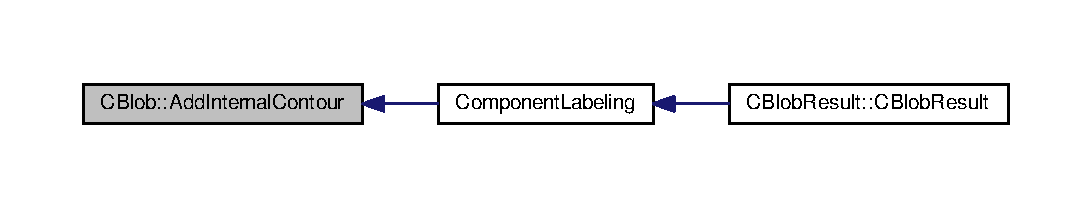
\includegraphics[width=350pt]{classCBlob_ad26a1bc4e31809c3bd76424b05824e90_icgraph}
\end{center}
\end{figure}


\hypertarget{classCBlob_a6f1db9fcb42c0a3ea003aaeb0ec65a8d}{\index{C\-Blob@{C\-Blob}!Area@{Area}}
\index{Area@{Area}!CBlob@{C\-Blob}}
\subsubsection[{Area}]{\setlength{\rightskip}{0pt plus 5cm}double C\-Blob\-::\-Area (
\begin{DoxyParamCaption}
{}
\end{DoxyParamCaption}
)}}\label{classCBlob_a6f1db9fcb42c0a3ea003aaeb0ec65a8d}


Compute blob's area. 


\begin{DoxyItemize}
\item F\-U\-N\-C\-I�\-: Area
\item F\-U\-N\-C\-I\-O\-N\-A\-L\-I\-T\-A\-T\-: Get blob area, ie. external contour area minus internal contours area
\item P\-A\-R�\-M\-E\-T\-R\-E\-S\-:
\begin{DoxyItemize}
\item 
\end{DoxyItemize}
\item R\-E\-S\-U\-L\-T\-A\-T\-:
\begin{DoxyItemize}
\item 
\end{DoxyItemize}
\item R\-E\-S\-T\-R\-I\-C\-C\-I\-O\-N\-S\-:
\begin{DoxyItemize}
\item 
\end{DoxyItemize}
\item A\-U\-T\-O\-R\-: rborras
\item D\-A\-T\-A D\-E C\-R\-E\-A\-C\-I�\-: 2008/04/30
\item M\-O\-D\-I\-F\-I\-C\-A\-C\-I�\-: Data. Autor. Descripci�. 
\end{DoxyItemize}

Here is the call graph for this function\-:\nopagebreak
\begin{figure}[H]
\begin{center}
\leavevmode
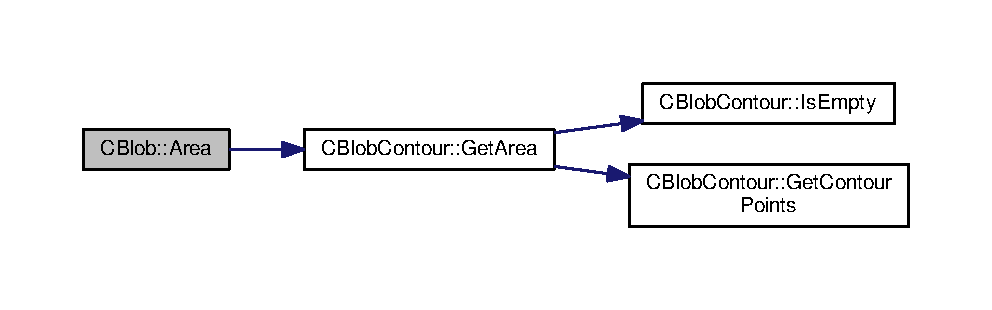
\includegraphics[width=350pt]{classCBlob_a6f1db9fcb42c0a3ea003aaeb0ec65a8d_cgraph}
\end{center}
\end{figure}




Here is the caller graph for this function\-:\nopagebreak
\begin{figure}[H]
\begin{center}
\leavevmode
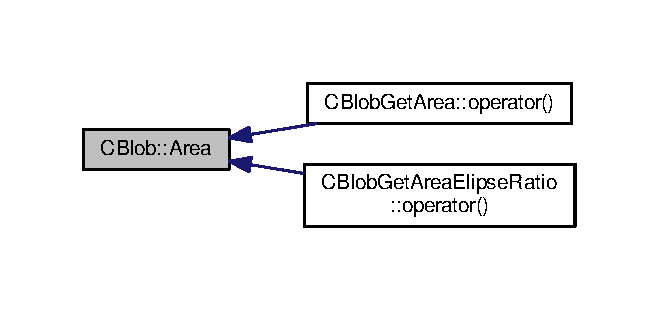
\includegraphics[width=316pt]{classCBlob_a6f1db9fcb42c0a3ea003aaeb0ec65a8d_icgraph}
\end{center}
\end{figure}


\hypertarget{classCBlob_a4e3c8e5c89036d0a141ca8f839e4e7e3}{\index{C\-Blob@{C\-Blob}!Clear\-Contours@{Clear\-Contours}}
\index{Clear\-Contours@{Clear\-Contours}!CBlob@{C\-Blob}}
\subsubsection[{Clear\-Contours}]{\setlength{\rightskip}{0pt plus 5cm}void C\-Blob\-::\-Clear\-Contours (
\begin{DoxyParamCaption}
{}
\end{DoxyParamCaption}
)\hspace{0.3cm}{\ttfamily [private]}}}\label{classCBlob_a4e3c8e5c89036d0a141ca8f839e4e7e3}


Deallocates all contours. 



Here is the call graph for this function\-:\nopagebreak
\begin{figure}[H]
\begin{center}
\leavevmode
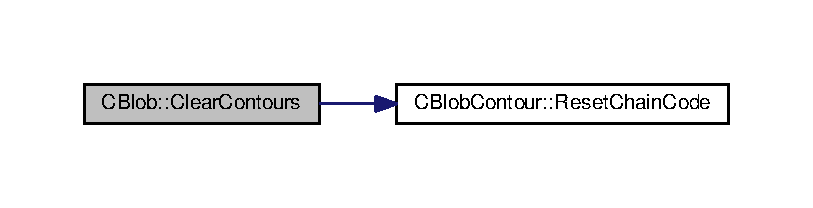
\includegraphics[width=350pt]{classCBlob_a4e3c8e5c89036d0a141ca8f839e4e7e3_cgraph}
\end{center}
\end{figure}




Here is the caller graph for this function\-:\nopagebreak
\begin{figure}[H]
\begin{center}
\leavevmode
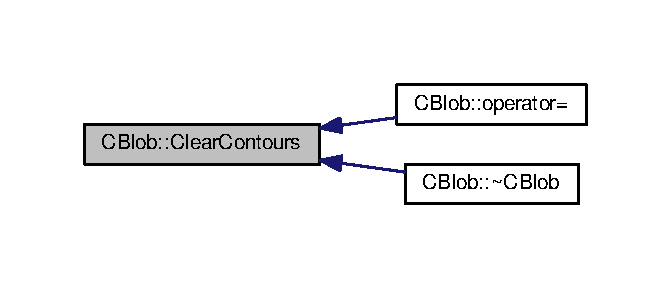
\includegraphics[width=322pt]{classCBlob_a4e3c8e5c89036d0a141ca8f839e4e7e3_icgraph}
\end{center}
\end{figure}


\hypertarget{classCBlob_a2d56a7dee1cbeb3178ff083630ee31b0}{\index{C\-Blob@{C\-Blob}!Exterior@{Exterior}}
\index{Exterior@{Exterior}!CBlob@{C\-Blob}}
\subsubsection[{Exterior}]{\setlength{\rightskip}{0pt plus 5cm}int C\-Blob\-::\-Exterior (
\begin{DoxyParamCaption}
\item[{Ipl\-Image $\ast$}]{mask, }
\item[{bool}]{x\-Border = {\ttfamily true}, }
\item[{bool}]{y\-Border = {\ttfamily true}}
\end{DoxyParamCaption}
)}}\label{classCBlob_a2d56a7dee1cbeb3178ff083630ee31b0}


\begin{quotation}
0 for extern blobs, 0 if not \end{quotation}



\begin{DoxyItemize}
\item F\-U\-N\-C\-I�\-: Exterior
\item F\-U\-N\-C\-I\-O\-N\-A\-L\-I\-T\-A\-T\-: Return true for extern blobs
\item P\-A\-R�\-M\-E\-T\-R\-E\-S\-:
\begin{DoxyItemize}
\item x\-Border\-: true to consider blobs touching horizontal borders as extern
\item y\-Border\-: true to consider blobs touching vertical borders as extern
\end{DoxyItemize}
\item R\-E\-S\-U\-L\-T\-A\-T\-:
\begin{DoxyItemize}
\item 
\end{DoxyItemize}
\item R\-E\-S\-T\-R\-I\-C\-C\-I\-O\-N\-S\-:
\begin{DoxyItemize}
\item 
\end{DoxyItemize}
\item A\-U\-T\-O\-R\-: rborras
\item D\-A\-T\-A D\-E C\-R\-E\-A\-C\-I�\-: 2008/05/06
\item M\-O\-D\-I\-F\-I\-C\-A\-C\-I�\-: Data. Autor. Descripci�. 
\end{DoxyItemize}

Here is the call graph for this function\-:\nopagebreak
\begin{figure}[H]
\begin{center}
\leavevmode
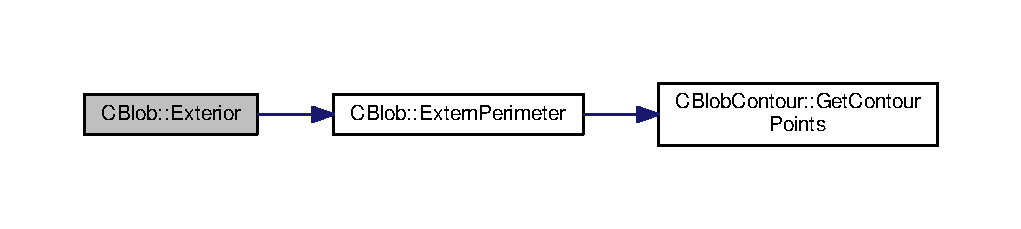
\includegraphics[width=350pt]{classCBlob_a2d56a7dee1cbeb3178ff083630ee31b0_cgraph}
\end{center}
\end{figure}




Here is the caller graph for this function\-:\nopagebreak
\begin{figure}[H]
\begin{center}
\leavevmode
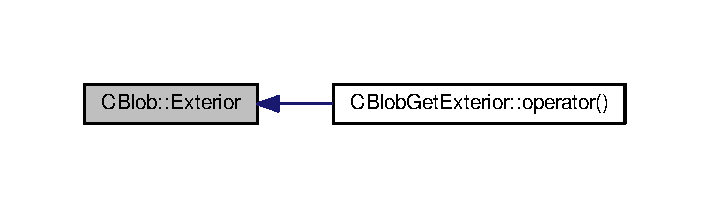
\includegraphics[width=340pt]{classCBlob_a2d56a7dee1cbeb3178ff083630ee31b0_icgraph}
\end{center}
\end{figure}


\hypertarget{classCBlob_ab1501b07a2c5ee23843bac66d20974e2}{\index{C\-Blob@{C\-Blob}!Extern\-Perimeter@{Extern\-Perimeter}}
\index{Extern\-Perimeter@{Extern\-Perimeter}!CBlob@{C\-Blob}}
\subsubsection[{Extern\-Perimeter}]{\setlength{\rightskip}{0pt plus 5cm}double C\-Blob\-::\-Extern\-Perimeter (
\begin{DoxyParamCaption}
\item[{Ipl\-Image $\ast$}]{mask\-Image, }
\item[{bool}]{x\-Border = {\ttfamily true}, }
\item[{bool}]{y\-Border = {\ttfamily true}}
\end{DoxyParamCaption}
)}}\label{classCBlob_ab1501b07a2c5ee23843bac66d20974e2}


Compute extern perimeter. 


\begin{DoxyItemize}
\item F\-U\-N\-C\-I�\-: Extern\-Perimeter
\item F\-U\-N\-C\-I\-O\-N\-A\-L\-I\-T\-A\-T\-: Get extern perimeter (perimeter touching image borders)
\item P\-A\-R�\-M\-E\-T\-R\-E\-S\-:
\begin{DoxyItemize}
\item mask\-Image\-: if != N\-U\-L\-L, counts mask\-Image black pixels as external pixels and contour points touching them are counted as external contour points.
\item x\-Border\-: true to consider blobs touching horizontal borders as extern
\item y\-Border\-: true to consider blobs touching vertical borders as extern
\end{DoxyItemize}
\item R\-E\-S\-U\-L\-T\-A\-T\-:
\begin{DoxyItemize}
\item 
\end{DoxyItemize}
\item R\-E\-S\-T\-R\-I\-C\-C\-I\-O\-N\-S\-:
\begin{DoxyItemize}
\item 
\end{DoxyItemize}
\item A\-U\-T\-O\-R\-: rborras
\item D\-A\-T\-A D\-E C\-R\-E\-A\-C\-I�\-: 2008/05/05
\item M\-O\-D\-I\-F\-I\-C\-A\-C\-I�\-: Data. Autor. Descripci�.
\item N\-O\-T\-A\-: If \hyperlink{classCBlobContour_a245d5e59180619aa9ae4ec14acc18744}{C\-Blob\-Contour\-::\-Get\-Contour\-Points} aproximates contours with a method different that N\-O\-N\-E, this function will not give correct results 
\end{DoxyItemize}

Here is the call graph for this function\-:\nopagebreak
\begin{figure}[H]
\begin{center}
\leavevmode
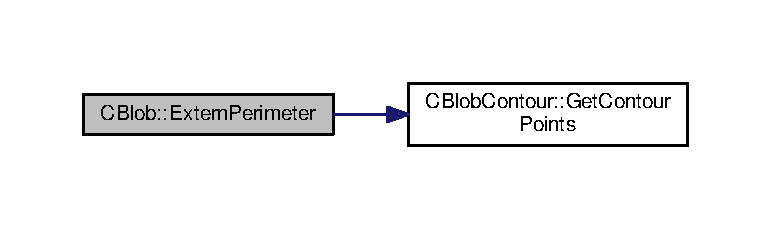
\includegraphics[width=350pt]{classCBlob_ab1501b07a2c5ee23843bac66d20974e2_cgraph}
\end{center}
\end{figure}




Here is the caller graph for this function\-:\nopagebreak
\begin{figure}[H]
\begin{center}
\leavevmode
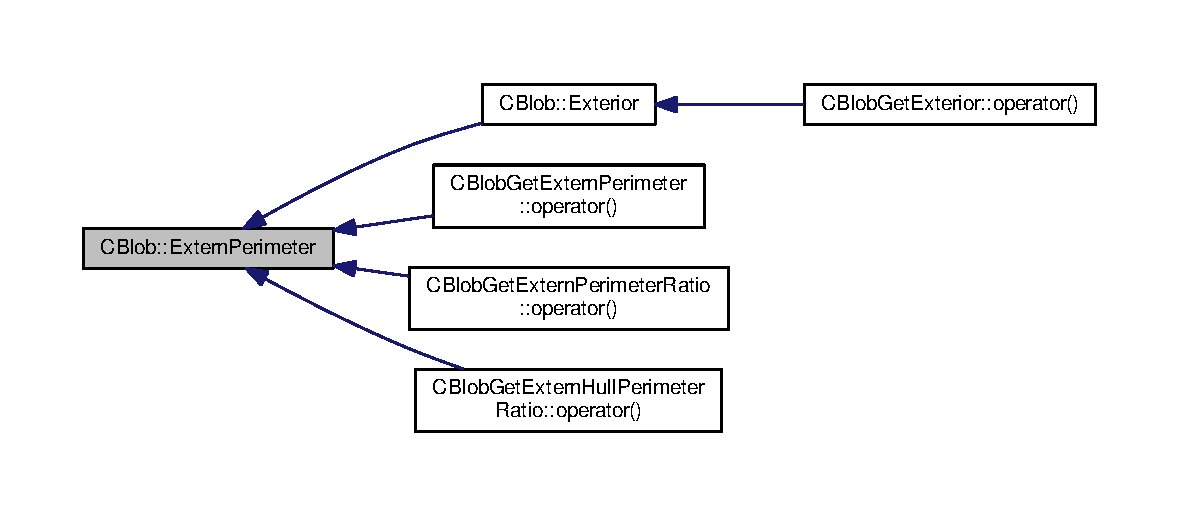
\includegraphics[width=350pt]{classCBlob_ab1501b07a2c5ee23843bac66d20974e2_icgraph}
\end{center}
\end{figure}


\hypertarget{classCBlob_a1a12b6dee61d2db86cd3a60c0671382e}{\index{C\-Blob@{C\-Blob}!Fill\-Blob@{Fill\-Blob}}
\index{Fill\-Blob@{Fill\-Blob}!CBlob@{C\-Blob}}
\subsubsection[{Fill\-Blob}]{\setlength{\rightskip}{0pt plus 5cm}void C\-Blob\-::\-Fill\-Blob (
\begin{DoxyParamCaption}
\item[{Ipl\-Image $\ast$}]{imatge, }
\item[{Cv\-Scalar}]{color, }
\item[{int}]{offset\-X = {\ttfamily 0}, }
\item[{int}]{offset\-Y = {\ttfamily 0}}
\end{DoxyParamCaption}
)}}\label{classCBlob_a1a12b6dee61d2db86cd3a60c0671382e}
Pinta l'interior d'un blob d'un color determinat Paints the blob in an image


\begin{DoxyItemize}
\item F\-U\-N\-C\-T\-I\-O\-N\-: Fill\-Blob
\item F\-U\-N\-C\-T\-I\-O\-N\-A\-L\-I\-T\-Y\-:
\begin{DoxyItemize}
\item Fills the blob with a specified colour
\end{DoxyItemize}
\item P\-A\-R\-A\-M\-E\-T\-E\-R\-S\-:
\begin{DoxyItemize}
\item imatge\-: where to paint
\item color\-: colour to paint the blob
\end{DoxyItemize}
\item R\-E\-S\-U\-L\-T\-:
\begin{DoxyItemize}
\item modifies input image and returns the seed point used to fill the blob
\end{DoxyItemize}
\item R\-E\-S\-T\-R\-I\-C\-T\-I\-O\-N\-S\-:
\item A\-U\-T\-H\-O\-R\-: Ricard Borr�s
\item C\-R\-E\-A\-T\-I\-O\-N D\-A\-T\-E\-: 25-\/05-\/2005.
\item M\-O\-D\-I\-F\-I\-C\-A\-T\-I\-O\-N\-: Date. Author. Description. 
\end{DoxyItemize}

Here is the call graph for this function\-:\nopagebreak
\begin{figure}[H]
\begin{center}
\leavevmode
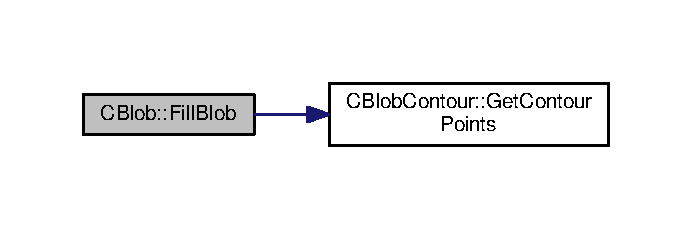
\includegraphics[width=332pt]{classCBlob_a1a12b6dee61d2db86cd3a60c0671382e_cgraph}
\end{center}
\end{figure}


\hypertarget{classCBlob_a5391167c172eb461eb762fbdd81306de}{\index{C\-Blob@{C\-Blob}!Get\-Bounding\-Box@{Get\-Bounding\-Box}}
\index{Get\-Bounding\-Box@{Get\-Bounding\-Box}!CBlob@{C\-Blob}}
\subsubsection[{Get\-Bounding\-Box}]{\setlength{\rightskip}{0pt plus 5cm}Cv\-Rect C\-Blob\-::\-Get\-Bounding\-Box (
\begin{DoxyParamCaption}
{}
\end{DoxyParamCaption}
)}}\label{classCBlob_a5391167c172eb461eb762fbdd81306de}


Get bounding box. 


\begin{DoxyItemize}
\item F\-U\-N\-C\-I�\-: Get\-Bounding\-Box
\item F\-U\-N\-C\-I\-O\-N\-A\-L\-I\-T\-A\-T\-: Get bounding box (without rotation) of a blob
\item P\-A\-R�\-M\-E\-T\-R\-E\-S\-:
\begin{DoxyItemize}
\item 
\end{DoxyItemize}
\item R\-E\-S\-U\-L\-T\-A\-T\-:
\begin{DoxyItemize}
\item 
\end{DoxyItemize}
\item R\-E\-S\-T\-R\-I\-C\-C\-I\-O\-N\-S\-:
\begin{DoxyItemize}
\item 
\end{DoxyItemize}
\item A\-U\-T\-O\-R\-: rborras
\item D\-A\-T\-A D\-E C\-R\-E\-A\-C\-I�\-: 2008/05/06
\item M\-O\-D\-I\-F\-I\-C\-A\-C\-I�\-: Data. Autor. Descripci�. 
\end{DoxyItemize}

Here is the call graph for this function\-:\nopagebreak
\begin{figure}[H]
\begin{center}
\leavevmode
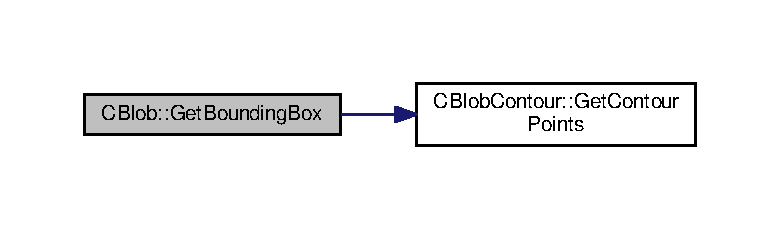
\includegraphics[width=350pt]{classCBlob_a5391167c172eb461eb762fbdd81306de_cgraph}
\end{center}
\end{figure}




Here is the caller graph for this function\-:\nopagebreak
\begin{figure}[H]
\begin{center}
\leavevmode
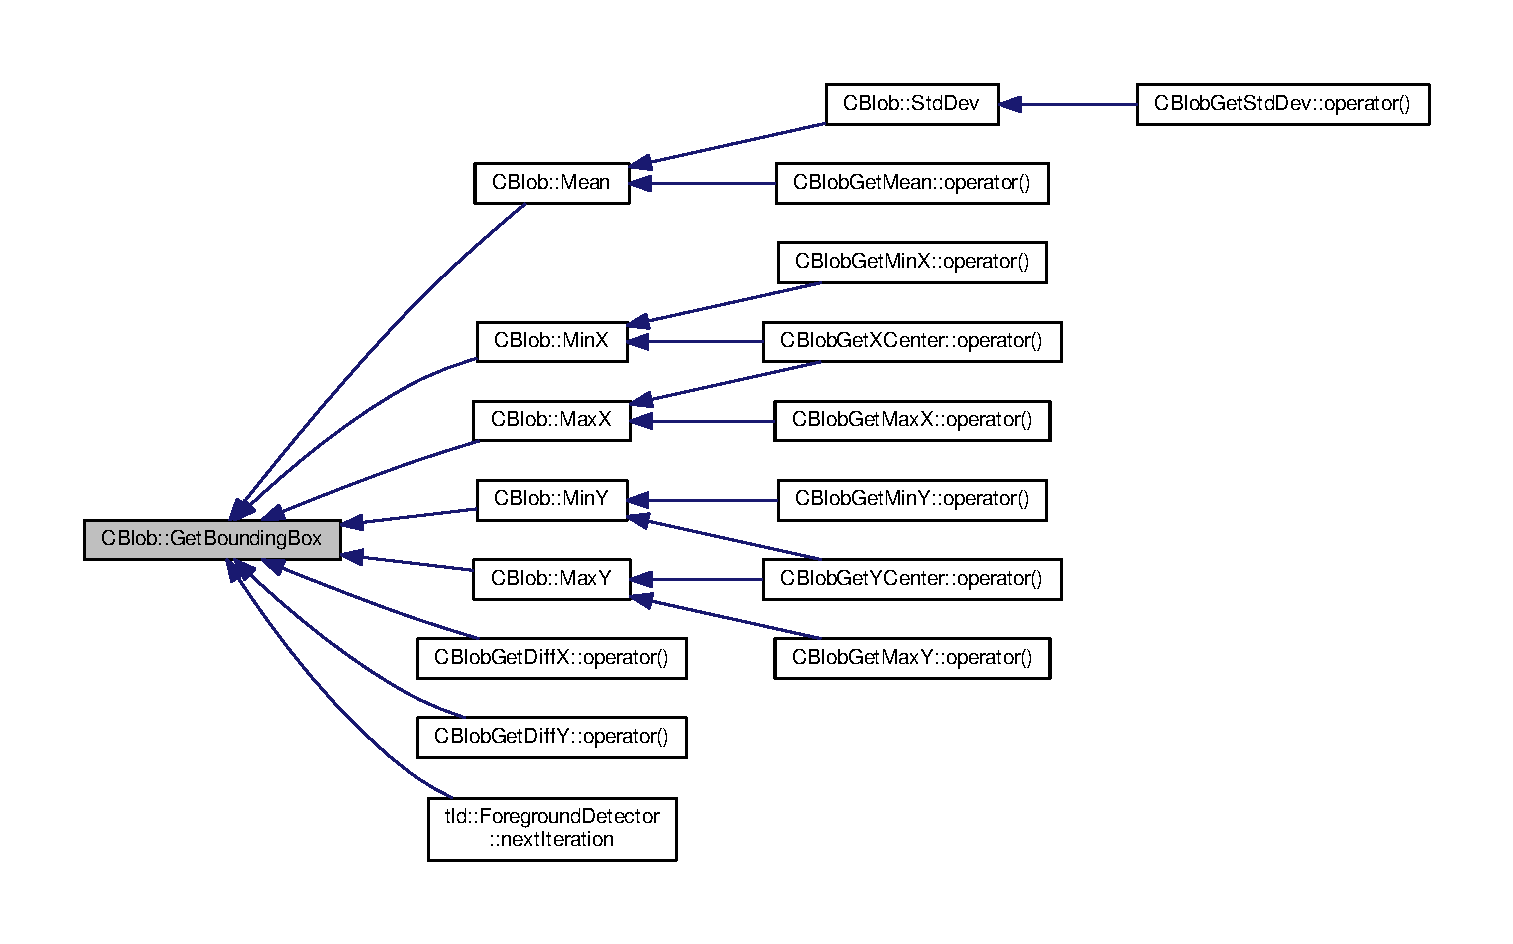
\includegraphics[width=350pt]{classCBlob_a5391167c172eb461eb762fbdd81306de_icgraph}
\end{center}
\end{figure}


\hypertarget{classCBlob_aacc50d5d47e0543d4e0a569d05009006}{\index{C\-Blob@{C\-Blob}!Get\-Convex\-Hull@{Get\-Convex\-Hull}}
\index{Get\-Convex\-Hull@{Get\-Convex\-Hull}!CBlob@{C\-Blob}}
\subsubsection[{Get\-Convex\-Hull}]{\setlength{\rightskip}{0pt plus 5cm}{\bf t\-\_\-\-Point\-List} C\-Blob\-::\-Get\-Convex\-Hull (
\begin{DoxyParamCaption}
{}
\end{DoxyParamCaption}
)}}\label{classCBlob_aacc50d5d47e0543d4e0a569d05009006}
Retorna el poligon convex del blob Calculates the convex hull of the blob


\begin{DoxyItemize}
\item F\-U\-N\-C\-T\-I\-O\-N\-: Get\-Convex\-Hull
\item F\-U\-N\-C\-T\-I\-O\-N\-A\-L\-I\-T\-Y\-: Calculates the convex hull polygon of the blob
\item P\-A\-R\-A\-M\-E\-T\-E\-R\-S\-:
\begin{DoxyItemize}
\item dst\-: where to store the result
\end{DoxyItemize}
\item R\-E\-S\-U\-L\-T\-:
\begin{DoxyItemize}
\item true if no error ocurred
\end{DoxyItemize}
\item R\-E\-S\-T\-R\-I\-C\-T\-I\-O\-N\-S\-:
\item A\-U\-T\-H\-O\-R\-: Ricard Borr�s
\item C\-R\-E\-A\-T\-I\-O\-N D\-A\-T\-E\-: 25-\/05-\/2005.
\item M\-O\-D\-I\-F\-I\-C\-A\-T\-I\-O\-N\-: Date. Author. Description. 
\end{DoxyItemize}

Here is the call graph for this function\-:\nopagebreak
\begin{figure}[H]
\begin{center}
\leavevmode
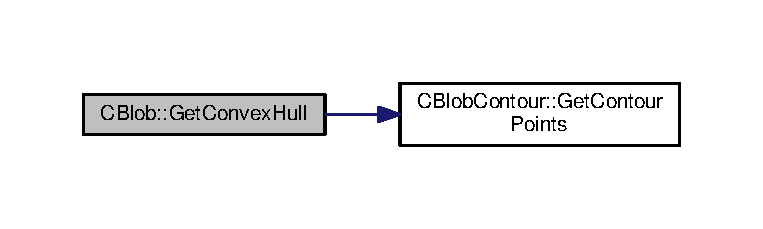
\includegraphics[width=350pt]{classCBlob_aacc50d5d47e0543d4e0a569d05009006_cgraph}
\end{center}
\end{figure}


\hypertarget{classCBlob_ad0bb95f395084ee89ca35cf11f203342}{\index{C\-Blob@{C\-Blob}!Get\-Ellipse@{Get\-Ellipse}}
\index{Get\-Ellipse@{Get\-Ellipse}!CBlob@{C\-Blob}}
\subsubsection[{Get\-Ellipse}]{\setlength{\rightskip}{0pt plus 5cm}Cv\-Box2\-D C\-Blob\-::\-Get\-Ellipse (
\begin{DoxyParamCaption}
{}
\end{DoxyParamCaption}
)}}\label{classCBlob_ad0bb95f395084ee89ca35cf11f203342}


Get bounding ellipse. 


\begin{DoxyItemize}
\item F\-U\-N\-C\-I�\-: Get\-Ellipse
\item F\-U\-N\-C\-I\-O\-N\-A\-L\-I\-T\-A\-T\-: Calculates bounding ellipse of external contour points
\item P\-A\-R�\-M\-E\-T\-R\-E\-S\-:
\begin{DoxyItemize}
\item 
\end{DoxyItemize}
\item R\-E\-S\-U\-L\-T\-A\-T\-:
\begin{DoxyItemize}
\item 
\end{DoxyItemize}
\item R\-E\-S\-T\-R\-I\-C\-C\-I\-O\-N\-S\-:
\begin{DoxyItemize}
\item 
\end{DoxyItemize}
\item A\-U\-T\-O\-R\-: rborras
\item D\-A\-T\-A D\-E C\-R\-E\-A\-C\-I�\-: 2008/05/06
\item M\-O\-D\-I\-F\-I\-C\-A\-C\-I�\-: Data. Autor. Descripci�.
\item N\-O\-T\-A\-: Calculation is made using second order moment aproximation 
\end{DoxyItemize}

Here is the call graph for this function\-:\nopagebreak
\begin{figure}[H]
\begin{center}
\leavevmode
\includegraphics[width=350pt]{classCBlob_ad0bb95f395084ee89ca35cf11f203342_cgraph}
\end{center}
\end{figure}




Here is the caller graph for this function\-:\nopagebreak
\begin{figure}[H]
\begin{center}
\leavevmode
\includegraphics[width=344pt]{classCBlob_ad0bb95f395084ee89ca35cf11f203342_icgraph}
\end{center}
\end{figure}


\hypertarget{classCBlob_ad136387165bd74c368cb4ecc7632e4cf}{\index{C\-Blob@{C\-Blob}!Get\-External\-Contour@{Get\-External\-Contour}}
\index{Get\-External\-Contour@{Get\-External\-Contour}!CBlob@{C\-Blob}}
\subsubsection[{Get\-External\-Contour}]{\setlength{\rightskip}{0pt plus 5cm}{\bf C\-Blob\-Contour}$\ast$ C\-Blob\-::\-Get\-External\-Contour (
\begin{DoxyParamCaption}
{}
\end{DoxyParamCaption}
)\hspace{0.3cm}{\ttfamily [inline]}}}\label{classCBlob_ad136387165bd74c368cb4ecc7632e4cf}


Retrieves contour in Freeman's chain code. 



Here is the caller graph for this function\-:\nopagebreak
\begin{figure}[H]
\begin{center}
\leavevmode
\includegraphics[width=350pt]{classCBlob_ad136387165bd74c368cb4ecc7632e4cf_icgraph}
\end{center}
\end{figure}


\hypertarget{classCBlob_a1d3fd90bc98f6d845babb18a3f058bc2}{\index{C\-Blob@{C\-Blob}!Get\-I\-D@{Get\-I\-D}}
\index{Get\-I\-D@{Get\-I\-D}!CBlob@{C\-Blob}}
\subsubsection[{Get\-I\-D}]{\setlength{\rightskip}{0pt plus 5cm}{\bf t\-\_\-label\-Type} C\-Blob\-::\-Get\-I\-D (
\begin{DoxyParamCaption}
{}
\end{DoxyParamCaption}
)\hspace{0.3cm}{\ttfamily [inline]}}}\label{classCBlob_a1d3fd90bc98f6d845babb18a3f058bc2}


Get label I\-D. 



Here is the caller graph for this function\-:\nopagebreak
\begin{figure}[H]
\begin{center}
\leavevmode
\includegraphics[width=310pt]{classCBlob_a1d3fd90bc98f6d845babb18a3f058bc2_icgraph}
\end{center}
\end{figure}


\hypertarget{classCBlob_a1eeee72a4369dc9485c6ae6573631a02}{\index{C\-Blob@{C\-Blob}!Get\-Storage@{Get\-Storage}}
\index{Get\-Storage@{Get\-Storage}!CBlob@{C\-Blob}}
\subsubsection[{Get\-Storage}]{\setlength{\rightskip}{0pt plus 5cm}Cv\-Mem\-Storage$\ast$ C\-Blob\-::\-Get\-Storage (
\begin{DoxyParamCaption}
{}
\end{DoxyParamCaption}
)\hspace{0.3cm}{\ttfamily [inline]}}}\label{classCBlob_a1eeee72a4369dc9485c6ae6573631a02}


Retrieves blob storage. 



Here is the caller graph for this function\-:\nopagebreak
\begin{figure}[H]
\begin{center}
\leavevmode
\includegraphics[width=350pt]{classCBlob_a1eeee72a4369dc9485c6ae6573631a02_icgraph}
\end{center}
\end{figure}


\hypertarget{classCBlob_ac97e73d3040530de09a187d02632deb1}{\index{C\-Blob@{C\-Blob}!Is\-Empty@{Is\-Empty}}
\index{Is\-Empty@{Is\-Empty}!CBlob@{C\-Blob}}
\subsubsection[{Is\-Empty}]{\setlength{\rightskip}{0pt plus 5cm}bool C\-Blob\-::\-Is\-Empty (
\begin{DoxyParamCaption}
{}
\end{DoxyParamCaption}
)}}\label{classCBlob_ac97e73d3040530de09a187d02632deb1}
Indica si el blob est� buit ( no t� cap info associada ) Shows if the blob has associated information 

Here is the call graph for this function\-:\nopagebreak
\begin{figure}[H]
\begin{center}
\leavevmode
\includegraphics[width=338pt]{classCBlob_ac97e73d3040530de09a187d02632deb1_cgraph}
\end{center}
\end{figure}


\hypertarget{classCBlob_a006463cc42ef0e4b8986fa5020cb6f90}{\index{C\-Blob@{C\-Blob}!Join\-Blob@{Join\-Blob}}
\index{Join\-Blob@{Join\-Blob}!CBlob@{C\-Blob}}
\subsubsection[{Join\-Blob}]{\setlength{\rightskip}{0pt plus 5cm}void C\-Blob\-::\-Join\-Blob (
\begin{DoxyParamCaption}
\item[{{\bf C\-Blob} $\ast$}]{blob}
\end{DoxyParamCaption}
)}}\label{classCBlob_a006463cc42ef0e4b8986fa5020cb6f90}


Join a blob to current one (add's contour. 


\begin{DoxyItemize}
\item F\-U\-N\-C\-T\-I\-O\-N\-: Join\-Blob
\item F\-U\-N\-C\-T\-I\-O\-N\-A\-L\-I\-T\-Y\-: Add's external contour to current external contour
\item P\-A\-R\-A\-M\-E\-T\-E\-R\-S\-:
\begin{DoxyItemize}
\item blob\-: blob from which extract the added external contour
\end{DoxyItemize}
\item R\-E\-S\-U\-L\-T\-:
\begin{DoxyItemize}
\item true if no error ocurred
\end{DoxyItemize}
\item R\-E\-S\-T\-R\-I\-C\-T\-I\-O\-N\-S\-: Only external contours are added
\item A\-U\-T\-H\-O\-R\-: Ricard Borr�s
\item C\-R\-E\-A\-T\-I\-O\-N D\-A\-T\-E\-: 25-\/05-\/2005.
\item M\-O\-D\-I\-F\-I\-C\-A\-T\-I\-O\-N\-: Date. Author. Description. 
\end{DoxyItemize}

Here is the call graph for this function\-:\nopagebreak
\begin{figure}[H]
\begin{center}
\leavevmode
\includegraphics[width=350pt]{classCBlob_a006463cc42ef0e4b8986fa5020cb6f90_cgraph}
\end{center}
\end{figure}


\hypertarget{classCBlob_ab26a757fffc581df39620425de008cbc}{\index{C\-Blob@{C\-Blob}!Max\-X@{Max\-X}}
\index{Max\-X@{Max\-X}!CBlob@{C\-Blob}}
\subsubsection[{Max\-X}]{\setlength{\rightskip}{0pt plus 5cm}double C\-Blob\-::\-Max\-X (
\begin{DoxyParamCaption}
{}
\end{DoxyParamCaption}
)\hspace{0.3cm}{\ttfamily [inline]}}}\label{classCBlob_ab26a757fffc581df39620425de008cbc}


Maximun X. 



Here is the call graph for this function\-:\nopagebreak
\begin{figure}[H]
\begin{center}
\leavevmode
\includegraphics[width=350pt]{classCBlob_ab26a757fffc581df39620425de008cbc_cgraph}
\end{center}
\end{figure}




Here is the caller graph for this function\-:\nopagebreak
\begin{figure}[H]
\begin{center}
\leavevmode
\includegraphics[width=336pt]{classCBlob_ab26a757fffc581df39620425de008cbc_icgraph}
\end{center}
\end{figure}


\hypertarget{classCBlob_a740a37afcd841bf719587d2f0128c555}{\index{C\-Blob@{C\-Blob}!Max\-Y@{Max\-Y}}
\index{Max\-Y@{Max\-Y}!CBlob@{C\-Blob}}
\subsubsection[{Max\-Y}]{\setlength{\rightskip}{0pt plus 5cm}double C\-Blob\-::\-Max\-Y (
\begin{DoxyParamCaption}
{}
\end{DoxyParamCaption}
)\hspace{0.3cm}{\ttfamily [inline]}}}\label{classCBlob_a740a37afcd841bf719587d2f0128c555}


Maximun Y. 



Here is the call graph for this function\-:\nopagebreak
\begin{figure}[H]
\begin{center}
\leavevmode
\includegraphics[width=350pt]{classCBlob_a740a37afcd841bf719587d2f0128c555_cgraph}
\end{center}
\end{figure}




Here is the caller graph for this function\-:\nopagebreak
\begin{figure}[H]
\begin{center}
\leavevmode
\includegraphics[width=336pt]{classCBlob_a740a37afcd841bf719587d2f0128c555_icgraph}
\end{center}
\end{figure}


\hypertarget{classCBlob_a1b12d25f8e470fdd808ac2e3bfe9bad4}{\index{C\-Blob@{C\-Blob}!Mean@{Mean}}
\index{Mean@{Mean}!CBlob@{C\-Blob}}
\subsubsection[{Mean}]{\setlength{\rightskip}{0pt plus 5cm}double C\-Blob\-::\-Mean (
\begin{DoxyParamCaption}
\item[{Ipl\-Image $\ast$}]{image}
\end{DoxyParamCaption}
)}}\label{classCBlob_a1b12d25f8e470fdd808ac2e3bfe9bad4}


Get mean grey color. 


\begin{DoxyItemize}
\item F\-U\-N\-C\-I�\-: Mean
\item F\-U\-N\-C\-I\-O\-N\-A\-L\-I\-T\-A\-T\-: Get blob mean color in input image
\item P\-A\-R�\-M\-E\-T\-R\-E\-S\-:
\begin{DoxyItemize}
\item image\-: image from gray color are extracted
\end{DoxyItemize}
\item R\-E\-S\-U\-L\-T\-A\-T\-:
\begin{DoxyItemize}
\item 
\end{DoxyItemize}
\item R\-E\-S\-T\-R\-I\-C\-C\-I\-O\-N\-S\-:
\begin{DoxyItemize}
\item 
\end{DoxyItemize}
\item A\-U\-T\-O\-R\-: rborras
\item D\-A\-T\-A D\-E C\-R\-E\-A\-C\-I�\-: 2008/05/06
\item M\-O\-D\-I\-F\-I\-C\-A\-C\-I�\-: Data. Autor. Descripci�. 
\end{DoxyItemize}

Here is the call graph for this function\-:\nopagebreak
\begin{figure}[H]
\begin{center}
\leavevmode
\includegraphics[width=350pt]{classCBlob_a1b12d25f8e470fdd808ac2e3bfe9bad4_cgraph}
\end{center}
\end{figure}




Here is the caller graph for this function\-:\nopagebreak
\begin{figure}[H]
\begin{center}
\leavevmode
\includegraphics[width=350pt]{classCBlob_a1b12d25f8e470fdd808ac2e3bfe9bad4_icgraph}
\end{center}
\end{figure}


\hypertarget{classCBlob_aa3313af22e7f28d65ba245bc3b8a30bc}{\index{C\-Blob@{C\-Blob}!Min\-X@{Min\-X}}
\index{Min\-X@{Min\-X}!CBlob@{C\-Blob}}
\subsubsection[{Min\-X}]{\setlength{\rightskip}{0pt plus 5cm}double C\-Blob\-::\-Min\-X (
\begin{DoxyParamCaption}
{}
\end{DoxyParamCaption}
)\hspace{0.3cm}{\ttfamily [inline]}}}\label{classCBlob_aa3313af22e7f28d65ba245bc3b8a30bc}


Minimun X. 



Here is the call graph for this function\-:\nopagebreak
\begin{figure}[H]
\begin{center}
\leavevmode
\includegraphics[width=350pt]{classCBlob_aa3313af22e7f28d65ba245bc3b8a30bc_cgraph}
\end{center}
\end{figure}




Here is the caller graph for this function\-:\nopagebreak
\begin{figure}[H]
\begin{center}
\leavevmode
\includegraphics[width=332pt]{classCBlob_aa3313af22e7f28d65ba245bc3b8a30bc_icgraph}
\end{center}
\end{figure}


\hypertarget{classCBlob_a44e2caf6c7fc6e8360d2576c18c9bc2b}{\index{C\-Blob@{C\-Blob}!Min\-Y@{Min\-Y}}
\index{Min\-Y@{Min\-Y}!CBlob@{C\-Blob}}
\subsubsection[{Min\-Y}]{\setlength{\rightskip}{0pt plus 5cm}double C\-Blob\-::\-Min\-Y (
\begin{DoxyParamCaption}
{}
\end{DoxyParamCaption}
)\hspace{0.3cm}{\ttfamily [inline]}}}\label{classCBlob_a44e2caf6c7fc6e8360d2576c18c9bc2b}


Minimun Y. 



Here is the call graph for this function\-:\nopagebreak
\begin{figure}[H]
\begin{center}
\leavevmode
\includegraphics[width=350pt]{classCBlob_a44e2caf6c7fc6e8360d2576c18c9bc2b_cgraph}
\end{center}
\end{figure}




Here is the caller graph for this function\-:\nopagebreak
\begin{figure}[H]
\begin{center}
\leavevmode
\includegraphics[width=332pt]{classCBlob_a44e2caf6c7fc6e8360d2576c18c9bc2b_icgraph}
\end{center}
\end{figure}


\hypertarget{classCBlob_a4f5dfca1ee933e07a39965375f9f07c5}{\index{C\-Blob@{C\-Blob}!Moment@{Moment}}
\index{Moment@{Moment}!CBlob@{C\-Blob}}
\subsubsection[{Moment}]{\setlength{\rightskip}{0pt plus 5cm}double C\-Blob\-::\-Moment (
\begin{DoxyParamCaption}
\item[{int}]{p, }
\item[{int}]{q}
\end{DoxyParamCaption}
)}}\label{classCBlob_a4f5dfca1ee933e07a39965375f9f07c5}


Compute blob's moment (p,q up to M\-A\-X\-\_\-\-C\-A\-L\-C\-U\-L\-A\-T\-E\-D\-\_\-\-M\-O\-M\-E\-N\-T\-S) 



Here is the call graph for this function\-:\nopagebreak
\begin{figure}[H]
\begin{center}
\leavevmode
\includegraphics[width=350pt]{classCBlob_a4f5dfca1ee933e07a39965375f9f07c5_cgraph}
\end{center}
\end{figure}




Here is the caller graph for this function\-:\nopagebreak
\begin{figure}[H]
\begin{center}
\leavevmode
\includegraphics[width=350pt]{classCBlob_a4f5dfca1ee933e07a39965375f9f07c5_icgraph}
\end{center}
\end{figure}


\hypertarget{classCBlob_a724e55442a030bf94da856310e324a40}{\index{C\-Blob@{C\-Blob}!operator=@{operator=}}
\index{operator=@{operator=}!CBlob@{C\-Blob}}
\subsubsection[{operator=}]{\setlength{\rightskip}{0pt plus 5cm}{\bf C\-Blob} \& C\-Blob\-::operator= (
\begin{DoxyParamCaption}
\item[{const {\bf C\-Blob} \&}]{src}
\end{DoxyParamCaption}
)}}\label{classCBlob_a724e55442a030bf94da856310e324a40}
Operador d'assignaci� Assigment operator 

Here is the call graph for this function\-:\nopagebreak
\begin{figure}[H]
\begin{center}
\leavevmode
\includegraphics[width=350pt]{classCBlob_a724e55442a030bf94da856310e324a40_cgraph}
\end{center}
\end{figure}


\hypertarget{classCBlob_af63853ea55dbebbee5b013189e765b51}{\index{C\-Blob@{C\-Blob}!Perimeter@{Perimeter}}
\index{Perimeter@{Perimeter}!CBlob@{C\-Blob}}
\subsubsection[{Perimeter}]{\setlength{\rightskip}{0pt plus 5cm}double C\-Blob\-::\-Perimeter (
\begin{DoxyParamCaption}
{}
\end{DoxyParamCaption}
)}}\label{classCBlob_af63853ea55dbebbee5b013189e765b51}


Compute blob's perimeter. 


\begin{DoxyItemize}
\item F\-U\-N\-C\-I�\-: Perimeter
\item F\-U\-N\-C\-I\-O\-N\-A\-L\-I\-T\-A\-T\-: Get blob perimeter, ie. sum of the lenght of all the contours
\item P\-A\-R�\-M\-E\-T\-R\-E\-S\-:
\begin{DoxyItemize}
\item 
\end{DoxyItemize}
\item R\-E\-S\-U\-L\-T\-A\-T\-:
\begin{DoxyItemize}
\item 
\end{DoxyItemize}
\item R\-E\-S\-T\-R\-I\-C\-C\-I\-O\-N\-S\-:
\begin{DoxyItemize}
\item 
\end{DoxyItemize}
\item A\-U\-T\-O\-R\-: rborras
\item D\-A\-T\-A D\-E C\-R\-E\-A\-C\-I�\-: 2008/04/30
\item M\-O\-D\-I\-F\-I\-C\-A\-C\-I�\-: Data. Autor. Descripci�. 
\end{DoxyItemize}

Here is the call graph for this function\-:\nopagebreak
\begin{figure}[H]
\begin{center}
\leavevmode
\includegraphics[width=350pt]{classCBlob_af63853ea55dbebbee5b013189e765b51_cgraph}
\end{center}
\end{figure}




Here is the caller graph for this function\-:\nopagebreak
\begin{figure}[H]
\begin{center}
\leavevmode
\includegraphics[width=350pt]{classCBlob_af63853ea55dbebbee5b013189e765b51_icgraph}
\end{center}
\end{figure}


\hypertarget{classCBlob_a014b670bb748e6767ef070e1bc25be7a}{\index{C\-Blob@{C\-Blob}!Std\-Dev@{Std\-Dev}}
\index{Std\-Dev@{Std\-Dev}!CBlob@{C\-Blob}}
\subsubsection[{Std\-Dev}]{\setlength{\rightskip}{0pt plus 5cm}double C\-Blob\-::\-Std\-Dev (
\begin{DoxyParamCaption}
\item[{Ipl\-Image $\ast$}]{image}
\end{DoxyParamCaption}
)}}\label{classCBlob_a014b670bb748e6767ef070e1bc25be7a}


Get standard deviation grey color. 



Here is the call graph for this function\-:\nopagebreak
\begin{figure}[H]
\begin{center}
\leavevmode
\includegraphics[width=350pt]{classCBlob_a014b670bb748e6767ef070e1bc25be7a_cgraph}
\end{center}
\end{figure}




Here is the caller graph for this function\-:\nopagebreak
\begin{figure}[H]
\begin{center}
\leavevmode
\includegraphics[width=340pt]{classCBlob_a014b670bb748e6767ef070e1bc25be7a_icgraph}
\end{center}
\end{figure}




\subsection{Member Data Documentation}
\hypertarget{classCBlob_a9dd356b7cf492e6c8fa0109c81f6ac3c}{\index{C\-Blob@{C\-Blob}!m\-\_\-area@{m\-\_\-area}}
\index{m\-\_\-area@{m\-\_\-area}!CBlob@{C\-Blob}}
\subsubsection[{m\-\_\-area}]{\setlength{\rightskip}{0pt plus 5cm}double C\-Blob\-::m\-\_\-area\hspace{0.3cm}{\ttfamily [private]}}}\label{classCBlob_a9dd356b7cf492e6c8fa0109c81f6ac3c}


Area. 

\hypertarget{classCBlob_ad153da0682f927274e3493e0f0a8e9ff}{\index{C\-Blob@{C\-Blob}!m\-\_\-bounding\-Box@{m\-\_\-bounding\-Box}}
\index{m\-\_\-bounding\-Box@{m\-\_\-bounding\-Box}!CBlob@{C\-Blob}}
\subsubsection[{m\-\_\-bounding\-Box}]{\setlength{\rightskip}{0pt plus 5cm}Cv\-Rect C\-Blob\-::m\-\_\-bounding\-Box\hspace{0.3cm}{\ttfamily [private]}}}\label{classCBlob_ad153da0682f927274e3493e0f0a8e9ff}


Bounding box. 

\hypertarget{classCBlob_aa06a47b96675de402b95dbbff330f3f0}{\index{C\-Blob@{C\-Blob}!m\-\_\-ellipse@{m\-\_\-ellipse}}
\index{m\-\_\-ellipse@{m\-\_\-ellipse}!CBlob@{C\-Blob}}
\subsubsection[{m\-\_\-ellipse}]{\setlength{\rightskip}{0pt plus 5cm}Cv\-Box2\-D C\-Blob\-::m\-\_\-ellipse\hspace{0.3cm}{\ttfamily [private]}}}\label{classCBlob_aa06a47b96675de402b95dbbff330f3f0}


Bounding ellipse. 

\hypertarget{classCBlob_a6432d83f68a1c75464bb1c2f7450e4b5}{\index{C\-Blob@{C\-Blob}!m\-\_\-external\-Contour@{m\-\_\-external\-Contour}}
\index{m\-\_\-external\-Contour@{m\-\_\-external\-Contour}!CBlob@{C\-Blob}}
\subsubsection[{m\-\_\-external\-Contour}]{\setlength{\rightskip}{0pt plus 5cm}{\bf C\-Blob\-Contour} C\-Blob\-::m\-\_\-external\-Contour\hspace{0.3cm}{\ttfamily [private]}}}\label{classCBlob_a6432d83f68a1c75464bb1c2f7450e4b5}


External contour of the blob (crack codes) 

\hypertarget{classCBlob_adf1b82bc3602c5d08028730ee3a3d47e}{\index{C\-Blob@{C\-Blob}!m\-\_\-extern\-Perimeter@{m\-\_\-extern\-Perimeter}}
\index{m\-\_\-extern\-Perimeter@{m\-\_\-extern\-Perimeter}!CBlob@{C\-Blob}}
\subsubsection[{m\-\_\-extern\-Perimeter}]{\setlength{\rightskip}{0pt plus 5cm}double C\-Blob\-::m\-\_\-extern\-Perimeter\hspace{0.3cm}{\ttfamily [private]}}}\label{classCBlob_adf1b82bc3602c5d08028730ee3a3d47e}


Extern perimeter from blob. 

\hypertarget{classCBlob_aee7e60307972994de76d4128f08851c0}{\index{C\-Blob@{C\-Blob}!m\-\_\-id@{m\-\_\-id}}
\index{m\-\_\-id@{m\-\_\-id}!CBlob@{C\-Blob}}
\subsubsection[{m\-\_\-id}]{\setlength{\rightskip}{0pt plus 5cm}{\bf t\-\_\-label\-Type} C\-Blob\-::m\-\_\-id\hspace{0.3cm}{\ttfamily [private]}}}\label{classCBlob_aee7e60307972994de76d4128f08851c0}


Label number. 

\hypertarget{classCBlob_a88071948e0c48f4b256147df3a03a7de}{\index{C\-Blob@{C\-Blob}!m\-\_\-internal\-Contours@{m\-\_\-internal\-Contours}}
\index{m\-\_\-internal\-Contours@{m\-\_\-internal\-Contours}!CBlob@{C\-Blob}}
\subsubsection[{m\-\_\-internal\-Contours}]{\setlength{\rightskip}{0pt plus 5cm}{\bf t\-\_\-contour\-List} C\-Blob\-::m\-\_\-internal\-Contours\hspace{0.3cm}{\ttfamily [private]}}}\label{classCBlob_a88071948e0c48f4b256147df3a03a7de}


Internal contours (crack codes) 

\hypertarget{classCBlob_aeb1c6a7e54a529c9231a96cbe644c9d4}{\index{C\-Blob@{C\-Blob}!m\-\_\-mean\-Gray@{m\-\_\-mean\-Gray}}
\index{m\-\_\-mean\-Gray@{m\-\_\-mean\-Gray}!CBlob@{C\-Blob}}
\subsubsection[{m\-\_\-mean\-Gray}]{\setlength{\rightskip}{0pt plus 5cm}double C\-Blob\-::m\-\_\-mean\-Gray\hspace{0.3cm}{\ttfamily [private]}}}\label{classCBlob_aeb1c6a7e54a529c9231a96cbe644c9d4}


Mean gray color. 

\hypertarget{classCBlob_a0dc76004877e49c4607ecf3bea800d49}{\index{C\-Blob@{C\-Blob}!m\-\_\-original\-Image\-Size@{m\-\_\-original\-Image\-Size}}
\index{m\-\_\-original\-Image\-Size@{m\-\_\-original\-Image\-Size}!CBlob@{C\-Blob}}
\subsubsection[{m\-\_\-original\-Image\-Size}]{\setlength{\rightskip}{0pt plus 5cm}Cv\-Size C\-Blob\-::m\-\_\-original\-Image\-Size\hspace{0.3cm}{\ttfamily [private]}}}\label{classCBlob_a0dc76004877e49c4607ecf3bea800d49}


Sizes from image where blob is extracted. 

\hypertarget{classCBlob_a4d08eee6c8bb843469afa60834707bb8}{\index{C\-Blob@{C\-Blob}!m\-\_\-perimeter@{m\-\_\-perimeter}}
\index{m\-\_\-perimeter@{m\-\_\-perimeter}!CBlob@{C\-Blob}}
\subsubsection[{m\-\_\-perimeter}]{\setlength{\rightskip}{0pt plus 5cm}double C\-Blob\-::m\-\_\-perimeter\hspace{0.3cm}{\ttfamily [private]}}}\label{classCBlob_a4d08eee6c8bb843469afa60834707bb8}


Perimeter. 

\hypertarget{classCBlob_ab54c421db7988eef96af434d2cf0b0da}{\index{C\-Blob@{C\-Blob}!m\-\_\-std\-Dev\-Gray@{m\-\_\-std\-Dev\-Gray}}
\index{m\-\_\-std\-Dev\-Gray@{m\-\_\-std\-Dev\-Gray}!CBlob@{C\-Blob}}
\subsubsection[{m\-\_\-std\-Dev\-Gray}]{\setlength{\rightskip}{0pt plus 5cm}double C\-Blob\-::m\-\_\-std\-Dev\-Gray\hspace{0.3cm}{\ttfamily [private]}}}\label{classCBlob_ab54c421db7988eef96af434d2cf0b0da}


Standard deviation from gray color blob distribution. 

\hypertarget{classCBlob_aca7cb0f750e553fa34935ea927fd2122}{\index{C\-Blob@{C\-Blob}!m\-\_\-storage@{m\-\_\-storage}}
\index{m\-\_\-storage@{m\-\_\-storage}!CBlob@{C\-Blob}}
\subsubsection[{m\-\_\-storage}]{\setlength{\rightskip}{0pt plus 5cm}Cv\-Mem\-Storage$\ast$ C\-Blob\-::m\-\_\-storage\hspace{0.3cm}{\ttfamily [private]}}}\label{classCBlob_aca7cb0f750e553fa34935ea927fd2122}


Contour storage memory. 



The documentation for this class was generated from the following files\-:\begin{DoxyCompactItemize}
\item 
src/3rdparty/cvblobs/\hyperlink{blob_8h}{blob.\-h}\item 
src/3rdparty/cvblobs/\hyperlink{blob_8cpp}{blob.\-cpp}\end{DoxyCompactItemize}

\hypertarget{classCBlobContour}{\section{C\-Blob\-Contour Class Reference}
\label{classCBlobContour}\index{C\-Blob\-Contour@{C\-Blob\-Contour}}
}


Blob contour class (in crack code)  




{\ttfamily \#include $<$Blob\-Contour.\-h$>$}

\subsection*{Public Member Functions}
\begin{DoxyCompactItemize}
\item 
\hyperlink{classCBlobContour_a4cfb475c4e55945fe13618768bef57c7}{C\-Blob\-Contour} ()
\begin{DoxyCompactList}\small\item\em Constructors. \end{DoxyCompactList}\item 
\hyperlink{classCBlobContour_a66a78de7519f1e8ae7b92bdc30a726cc}{C\-Blob\-Contour} (Cv\-Point start\-Point, Cv\-Mem\-Storage $\ast$storage)
\item 
\hyperlink{classCBlobContour_a24b82910c8cfb9b0a31a3fb55fd29e28}{C\-Blob\-Contour} (\hyperlink{classCBlobContour}{C\-Blob\-Contour} $\ast$source)
\begin{DoxyCompactList}\small\item\em Copy constructor. \end{DoxyCompactList}\item 
\hyperlink{classCBlobContour_a24c825e7c0fab7e98237a2db60a7fc7a}{$\sim$\-C\-Blob\-Contour} ()
\item 
\hyperlink{classCBlobContour}{C\-Blob\-Contour} \& \hyperlink{classCBlobContour_a9ed6e0471a8d1b7d6c9a1465e539bbd4}{operator=} (const \hyperlink{classCBlobContour}{C\-Blob\-Contour} \&source)
\begin{DoxyCompactList}\small\item\em Assigment operator. \end{DoxyCompactList}\item 
void \hyperlink{classCBlobContour_a5a10813d71e48c52e099001e6581366c}{Add\-Chain\-Code} (\hyperlink{BlobContour_8h_a0ccb8765a7971147eaf6cafef4bd3c0e}{t\-\_\-chain\-Code} code)
\begin{DoxyCompactList}\small\item\em Add chain code to contour. \end{DoxyCompactList}\item 
\hyperlink{BlobContour_8h_af4605a71deb8fb5bf67011c89418c970}{t\-\_\-chain\-Code\-List} \hyperlink{classCBlobContour_ae783c063f2d89f4d06396b552c92f9a6}{Get\-Chain\-Code} ()
\begin{DoxyCompactList}\small\item\em Return freeman chain coded contour. \end{DoxyCompactList}\item 
bool \hyperlink{classCBlobContour_af4e715a94924d5dc1a0e67cf75818bb5}{Is\-Empty} ()
\item 
\hyperlink{BlobContour_8h_af4605a71deb8fb5bf67011c89418c970}{t\-\_\-chain\-Code\-List} \hyperlink{classCBlobContour_a245d5e59180619aa9ae4ec14acc18744}{Get\-Contour\-Points} ()
\begin{DoxyCompactList}\small\item\em Return all contour points. \end{DoxyCompactList}\end{DoxyCompactItemize}
\subsection*{Protected Member Functions}
\begin{DoxyCompactItemize}
\item 
Cv\-Point \hyperlink{classCBlobContour_ac8f0fbdce452ede583013e010ce0c8e3}{Get\-Start\-Point} () const 
\item 
void \hyperlink{classCBlobContour_a9a9ea170c2100586ca7bdb4227589fe9}{Reset\-Chain\-Code} ()
\begin{DoxyCompactList}\small\item\em Clears chain code contour. \end{DoxyCompactList}\item 
double \hyperlink{classCBlobContour_a2c68f462fc31a0e7add9a85b007fa42a}{Get\-Area} ()
\begin{DoxyCompactList}\small\item\em Computes area from contour. \end{DoxyCompactList}\item 
double \hyperlink{classCBlobContour_a893d57d625bb8f26f4a31ff0b66b8406}{Get\-Perimeter} ()
\begin{DoxyCompactList}\small\item\em Computes perimeter from contour. \end{DoxyCompactList}\item 
double \hyperlink{classCBlobContour_a301727633680b38714302593945b748f}{Get\-Moment} (int p, int q)
\begin{DoxyCompactList}\small\item\em Get contour moment (p,q up to M\-A\-X\-\_\-\-C\-A\-L\-C\-U\-L\-A\-T\-E\-D\-\_\-\-M\-O\-M\-E\-N\-T\-S) \end{DoxyCompactList}\end{DoxyCompactItemize}
\subsection*{Protected Attributes}
\begin{DoxyCompactItemize}
\item 
\hyperlink{BlobContour_8h_af4605a71deb8fb5bf67011c89418c970}{t\-\_\-chain\-Code\-List} \hyperlink{classCBlobContour_a98c36d7be8524da3976fad97b611123e}{m\-\_\-contour}
\begin{DoxyCompactList}\small\item\em Crack code list. \end{DoxyCompactList}\end{DoxyCompactItemize}
\subsection*{Private Attributes}
\begin{DoxyCompactItemize}
\item 
Cv\-Point \hyperlink{classCBlobContour_afe5180a7ce89174ef095d37455c5cab7}{m\-\_\-start\-Point}
\begin{DoxyCompactList}\small\item\em Starting point of the contour. \end{DoxyCompactList}\item 
\hyperlink{BlobContour_8h_abf72b29b2c653dd623e9b39a447809c0}{t\-\_\-\-Point\-List} \hyperlink{classCBlobContour_a828a1556bfe21818a83dd9e7ce0f15c8}{m\-\_\-contour\-Points}
\begin{DoxyCompactList}\small\item\em All points from the contour. \end{DoxyCompactList}\item 
double \hyperlink{classCBlobContour_abb127d27a1cf1b9a670165506ed32c7a}{m\-\_\-area}
\begin{DoxyCompactList}\small\item\em Computed area from contour. \end{DoxyCompactList}\item 
double \hyperlink{classCBlobContour_a23523e72cfb2f442e3afdc91b6021578}{m\-\_\-perimeter}
\begin{DoxyCompactList}\small\item\em Computed perimeter from contour. \end{DoxyCompactList}\item 
Cv\-Moments \hyperlink{classCBlobContour_acf0822fad2d18208d34b44e507d9ea6f}{m\-\_\-moments}
\begin{DoxyCompactList}\small\item\em Computed moments from contour. \end{DoxyCompactList}\item 
Cv\-Mem\-Storage $\ast$ \hyperlink{classCBlobContour_ac08cef4325eeecfa0b3d7cdab634156a}{m\-\_\-parent\-Storage}
\begin{DoxyCompactList}\small\item\em Pointer to storage. \end{DoxyCompactList}\end{DoxyCompactItemize}
\subsection*{Friends}
\begin{DoxyCompactItemize}
\item 
class \hyperlink{classCBlobContour_ae1a0519c97d58c87882ff9a1462ae464}{C\-Blob}
\item 
class \hyperlink{classCBlobContour_a107dcb6bc234839a49f6a53dde777713}{C\-Blob\-Properties}
\end{DoxyCompactItemize}


\subsection{Detailed Description}
Blob contour class (in crack code) 

\subsection{Constructor \& Destructor Documentation}
\hypertarget{classCBlobContour_a4cfb475c4e55945fe13618768bef57c7}{\index{C\-Blob\-Contour@{C\-Blob\-Contour}!C\-Blob\-Contour@{C\-Blob\-Contour}}
\index{C\-Blob\-Contour@{C\-Blob\-Contour}!CBlobContour@{C\-Blob\-Contour}}
\subsubsection[{C\-Blob\-Contour}]{\setlength{\rightskip}{0pt plus 5cm}C\-Blob\-Contour\-::\-C\-Blob\-Contour (
\begin{DoxyParamCaption}
{}
\end{DoxyParamCaption}
)}}\label{classCBlobContour_a4cfb475c4e55945fe13618768bef57c7}


Constructors. 

\hypertarget{classCBlobContour_a66a78de7519f1e8ae7b92bdc30a726cc}{\index{C\-Blob\-Contour@{C\-Blob\-Contour}!C\-Blob\-Contour@{C\-Blob\-Contour}}
\index{C\-Blob\-Contour@{C\-Blob\-Contour}!CBlobContour@{C\-Blob\-Contour}}
\subsubsection[{C\-Blob\-Contour}]{\setlength{\rightskip}{0pt plus 5cm}C\-Blob\-Contour\-::\-C\-Blob\-Contour (
\begin{DoxyParamCaption}
\item[{Cv\-Point}]{start\-Point, }
\item[{Cv\-Mem\-Storage $\ast$}]{storage}
\end{DoxyParamCaption}
)}}\label{classCBlobContour_a66a78de7519f1e8ae7b92bdc30a726cc}
\hypertarget{classCBlobContour_a24b82910c8cfb9b0a31a3fb55fd29e28}{\index{C\-Blob\-Contour@{C\-Blob\-Contour}!C\-Blob\-Contour@{C\-Blob\-Contour}}
\index{C\-Blob\-Contour@{C\-Blob\-Contour}!CBlobContour@{C\-Blob\-Contour}}
\subsubsection[{C\-Blob\-Contour}]{\setlength{\rightskip}{0pt plus 5cm}C\-Blob\-Contour\-::\-C\-Blob\-Contour (
\begin{DoxyParamCaption}
\item[{{\bf C\-Blob\-Contour} $\ast$}]{source}
\end{DoxyParamCaption}
)}}\label{classCBlobContour_a24b82910c8cfb9b0a31a3fb55fd29e28}


Copy constructor. 

\hypertarget{classCBlobContour_a24c825e7c0fab7e98237a2db60a7fc7a}{\index{C\-Blob\-Contour@{C\-Blob\-Contour}!$\sim$\-C\-Blob\-Contour@{$\sim$\-C\-Blob\-Contour}}
\index{$\sim$\-C\-Blob\-Contour@{$\sim$\-C\-Blob\-Contour}!CBlobContour@{C\-Blob\-Contour}}
\subsubsection[{$\sim$\-C\-Blob\-Contour}]{\setlength{\rightskip}{0pt plus 5cm}C\-Blob\-Contour\-::$\sim$\-C\-Blob\-Contour (
\begin{DoxyParamCaption}
{}
\end{DoxyParamCaption}
)}}\label{classCBlobContour_a24c825e7c0fab7e98237a2db60a7fc7a}


\subsection{Member Function Documentation}
\hypertarget{classCBlobContour_a5a10813d71e48c52e099001e6581366c}{\index{C\-Blob\-Contour@{C\-Blob\-Contour}!Add\-Chain\-Code@{Add\-Chain\-Code}}
\index{Add\-Chain\-Code@{Add\-Chain\-Code}!CBlobContour@{C\-Blob\-Contour}}
\subsubsection[{Add\-Chain\-Code}]{\setlength{\rightskip}{0pt plus 5cm}void C\-Blob\-Contour\-::\-Add\-Chain\-Code (
\begin{DoxyParamCaption}
\item[{{\bf t\-\_\-chain\-Code}}]{chaincode}
\end{DoxyParamCaption}
)}}\label{classCBlobContour_a5a10813d71e48c52e099001e6581366c}


Add chain code to contour. 


\begin{DoxyItemize}
\item F\-U\-N\-C\-I�\-: Add\-Chain\-Code
\item F\-U\-N\-C\-I\-O\-N\-A\-L\-I\-T\-A\-T\-: Add chain code to contour
\item P\-A\-R�\-M\-E\-T\-R\-E\-S\-:
\begin{DoxyItemize}
\item 
\end{DoxyItemize}
\item R\-E\-S\-U\-L\-T\-A\-T\-:
\begin{DoxyItemize}
\item 
\end{DoxyItemize}
\item R\-E\-S\-T\-R\-I\-C\-C\-I\-O\-N\-S\-:
\begin{DoxyItemize}
\item 
\end{DoxyItemize}
\item A\-U\-T\-O\-R\-: rborras
\item D\-A\-T\-A D\-E C\-R\-E\-A\-C\-I�\-: 2008/05/06
\item M\-O\-D\-I\-F\-I\-C\-A\-C\-I�\-: Data. Autor. Descripci�. 
\end{DoxyItemize}

Here is the caller graph for this function\-:\nopagebreak
\begin{figure}[H]
\begin{center}
\leavevmode
\includegraphics[width=350pt]{classCBlobContour_a5a10813d71e48c52e099001e6581366c_icgraph}
\end{center}
\end{figure}


\hypertarget{classCBlobContour_a2c68f462fc31a0e7add9a85b007fa42a}{\index{C\-Blob\-Contour@{C\-Blob\-Contour}!Get\-Area@{Get\-Area}}
\index{Get\-Area@{Get\-Area}!CBlobContour@{C\-Blob\-Contour}}
\subsubsection[{Get\-Area}]{\setlength{\rightskip}{0pt plus 5cm}double C\-Blob\-Contour\-::\-Get\-Area (
\begin{DoxyParamCaption}
{}
\end{DoxyParamCaption}
)\hspace{0.3cm}{\ttfamily [protected]}}}\label{classCBlobContour_a2c68f462fc31a0e7add9a85b007fa42a}


Computes area from contour. 


\begin{DoxyItemize}
\item F\-U\-N\-C\-I�\-: Get\-Area
\item F\-U\-N\-C\-I\-O\-N\-A\-L\-I\-T\-A\-T\-: Computes area from chain code
\item P\-A\-R�\-M\-E\-T\-R\-E\-S\-:
\begin{DoxyItemize}
\item 
\end{DoxyItemize}
\item R\-E\-S\-U\-L\-T\-A\-T\-:
\begin{DoxyItemize}
\item May give negative areas for clock wise contours
\end{DoxyItemize}
\item R\-E\-S\-T\-R\-I\-C\-C\-I\-O\-N\-S\-:
\begin{DoxyItemize}
\item 
\end{DoxyItemize}
\item A\-U\-T\-O\-R\-: rborras
\item D\-A\-T\-A D\-E C\-R\-E\-A\-C\-I�\-: 2008/04/30
\item M\-O\-D\-I\-F\-I\-C\-A\-C\-I�\-: Data. Autor. Descripci�.
\item N\-O\-T\-A\-: Algorithm derived from \char`\"{}\-Properties of contour codes\char`\"{}, G.\-R. Wilson 
\end{DoxyItemize}

Here is the call graph for this function\-:\nopagebreak
\begin{figure}[H]
\begin{center}
\leavevmode
\includegraphics[width=350pt]{classCBlobContour_a2c68f462fc31a0e7add9a85b007fa42a_cgraph}
\end{center}
\end{figure}




Here is the caller graph for this function\-:\nopagebreak
\begin{figure}[H]
\begin{center}
\leavevmode
\includegraphics[width=350pt]{classCBlobContour_a2c68f462fc31a0e7add9a85b007fa42a_icgraph}
\end{center}
\end{figure}


\hypertarget{classCBlobContour_ae783c063f2d89f4d06396b552c92f9a6}{\index{C\-Blob\-Contour@{C\-Blob\-Contour}!Get\-Chain\-Code@{Get\-Chain\-Code}}
\index{Get\-Chain\-Code@{Get\-Chain\-Code}!CBlobContour@{C\-Blob\-Contour}}
\subsubsection[{Get\-Chain\-Code}]{\setlength{\rightskip}{0pt plus 5cm}{\bf t\-\_\-chain\-Code\-List} C\-Blob\-Contour\-::\-Get\-Chain\-Code (
\begin{DoxyParamCaption}
{}
\end{DoxyParamCaption}
)\hspace{0.3cm}{\ttfamily [inline]}}}\label{classCBlobContour_ae783c063f2d89f4d06396b552c92f9a6}


Return freeman chain coded contour. 



Here is the caller graph for this function\-:\nopagebreak
\begin{figure}[H]
\begin{center}
\leavevmode
\includegraphics[width=350pt]{classCBlobContour_ae783c063f2d89f4d06396b552c92f9a6_icgraph}
\end{center}
\end{figure}


\hypertarget{classCBlobContour_a245d5e59180619aa9ae4ec14acc18744}{\index{C\-Blob\-Contour@{C\-Blob\-Contour}!Get\-Contour\-Points@{Get\-Contour\-Points}}
\index{Get\-Contour\-Points@{Get\-Contour\-Points}!CBlobContour@{C\-Blob\-Contour}}
\subsubsection[{Get\-Contour\-Points}]{\setlength{\rightskip}{0pt plus 5cm}{\bf t\-\_\-\-Point\-List} C\-Blob\-Contour\-::\-Get\-Contour\-Points (
\begin{DoxyParamCaption}
{}
\end{DoxyParamCaption}
)}}\label{classCBlobContour_a245d5e59180619aa9ae4ec14acc18744}


Return all contour points. 

Calculate contour points from crack codes. 

Here is the caller graph for this function\-:\nopagebreak
\begin{figure}[H]
\begin{center}
\leavevmode
\includegraphics[width=350pt]{classCBlobContour_a245d5e59180619aa9ae4ec14acc18744_icgraph}
\end{center}
\end{figure}


\hypertarget{classCBlobContour_a301727633680b38714302593945b748f}{\index{C\-Blob\-Contour@{C\-Blob\-Contour}!Get\-Moment@{Get\-Moment}}
\index{Get\-Moment@{Get\-Moment}!CBlobContour@{C\-Blob\-Contour}}
\subsubsection[{Get\-Moment}]{\setlength{\rightskip}{0pt plus 5cm}double C\-Blob\-Contour\-::\-Get\-Moment (
\begin{DoxyParamCaption}
\item[{int}]{p, }
\item[{int}]{q}
\end{DoxyParamCaption}
)\hspace{0.3cm}{\ttfamily [protected]}}}\label{classCBlobContour_a301727633680b38714302593945b748f}


Get contour moment (p,q up to M\-A\-X\-\_\-\-C\-A\-L\-C\-U\-L\-A\-T\-E\-D\-\_\-\-M\-O\-M\-E\-N\-T\-S) 



Here is the call graph for this function\-:\nopagebreak
\begin{figure}[H]
\begin{center}
\leavevmode
\includegraphics[width=350pt]{classCBlobContour_a301727633680b38714302593945b748f_cgraph}
\end{center}
\end{figure}




Here is the caller graph for this function\-:\nopagebreak
\begin{figure}[H]
\begin{center}
\leavevmode
\includegraphics[width=350pt]{classCBlobContour_a301727633680b38714302593945b748f_icgraph}
\end{center}
\end{figure}


\hypertarget{classCBlobContour_a893d57d625bb8f26f4a31ff0b66b8406}{\index{C\-Blob\-Contour@{C\-Blob\-Contour}!Get\-Perimeter@{Get\-Perimeter}}
\index{Get\-Perimeter@{Get\-Perimeter}!CBlobContour@{C\-Blob\-Contour}}
\subsubsection[{Get\-Perimeter}]{\setlength{\rightskip}{0pt plus 5cm}double C\-Blob\-Contour\-::\-Get\-Perimeter (
\begin{DoxyParamCaption}
{}
\end{DoxyParamCaption}
)\hspace{0.3cm}{\ttfamily [protected]}}}\label{classCBlobContour_a893d57d625bb8f26f4a31ff0b66b8406}


Computes perimeter from contour. 


\begin{DoxyItemize}
\item F\-U\-N\-C\-I�\-: Get\-Perimeter
\item F\-U\-N\-C\-I\-O\-N\-A\-L\-I\-T\-A\-T\-: Get perimeter from chain code. Diagonals sum sqrt(2) and horizontal and vertical codes 1
\item P\-A\-R�\-M\-E\-T\-R\-E\-S\-:
\begin{DoxyItemize}
\item 
\end{DoxyItemize}
\item R\-E\-S\-U\-L\-T\-A\-T\-:
\begin{DoxyItemize}
\item 
\end{DoxyItemize}
\item R\-E\-S\-T\-R\-I\-C\-C\-I\-O\-N\-S\-:
\begin{DoxyItemize}
\item 
\end{DoxyItemize}
\item A\-U\-T\-O\-R\-: rborras
\item D\-A\-T\-A D\-E C\-R\-E\-A\-C\-I�\-: 2008/04/30
\item M\-O\-D\-I\-F\-I\-C\-A\-C\-I�\-: Data. Autor. Descripci�.
\item N\-O\-T\-A\-: Algorithm derived from \char`\"{}\-Methods to estimate area and perimeters of blob-\/like objects\-: A comparison\char`\"{}, L.\-Yang 
\end{DoxyItemize}

Here is the call graph for this function\-:\nopagebreak
\begin{figure}[H]
\begin{center}
\leavevmode
\includegraphics[width=350pt]{classCBlobContour_a893d57d625bb8f26f4a31ff0b66b8406_cgraph}
\end{center}
\end{figure}




Here is the caller graph for this function\-:\nopagebreak
\begin{figure}[H]
\begin{center}
\leavevmode
\includegraphics[width=350pt]{classCBlobContour_a893d57d625bb8f26f4a31ff0b66b8406_icgraph}
\end{center}
\end{figure}


\hypertarget{classCBlobContour_ac8f0fbdce452ede583013e010ce0c8e3}{\index{C\-Blob\-Contour@{C\-Blob\-Contour}!Get\-Start\-Point@{Get\-Start\-Point}}
\index{Get\-Start\-Point@{Get\-Start\-Point}!CBlobContour@{C\-Blob\-Contour}}
\subsubsection[{Get\-Start\-Point}]{\setlength{\rightskip}{0pt plus 5cm}Cv\-Point C\-Blob\-Contour\-::\-Get\-Start\-Point (
\begin{DoxyParamCaption}
{}
\end{DoxyParamCaption}
) const\hspace{0.3cm}{\ttfamily [inline]}, {\ttfamily [protected]}}}\label{classCBlobContour_ac8f0fbdce452ede583013e010ce0c8e3}


Here is the caller graph for this function\-:\nopagebreak
\begin{figure}[H]
\begin{center}
\leavevmode
\includegraphics[width=350pt]{classCBlobContour_ac8f0fbdce452ede583013e010ce0c8e3_icgraph}
\end{center}
\end{figure}


\hypertarget{classCBlobContour_af4e715a94924d5dc1a0e67cf75818bb5}{\index{C\-Blob\-Contour@{C\-Blob\-Contour}!Is\-Empty@{Is\-Empty}}
\index{Is\-Empty@{Is\-Empty}!CBlobContour@{C\-Blob\-Contour}}
\subsubsection[{Is\-Empty}]{\setlength{\rightskip}{0pt plus 5cm}bool C\-Blob\-Contour\-::\-Is\-Empty (
\begin{DoxyParamCaption}
{}
\end{DoxyParamCaption}
)\hspace{0.3cm}{\ttfamily [inline]}}}\label{classCBlobContour_af4e715a94924d5dc1a0e67cf75818bb5}


Here is the caller graph for this function\-:\nopagebreak
\begin{figure}[H]
\begin{center}
\leavevmode
\includegraphics[width=350pt]{classCBlobContour_af4e715a94924d5dc1a0e67cf75818bb5_icgraph}
\end{center}
\end{figure}


\hypertarget{classCBlobContour_a9ed6e0471a8d1b7d6c9a1465e539bbd4}{\index{C\-Blob\-Contour@{C\-Blob\-Contour}!operator=@{operator=}}
\index{operator=@{operator=}!CBlobContour@{C\-Blob\-Contour}}
\subsubsection[{operator=}]{\setlength{\rightskip}{0pt plus 5cm}{\bf C\-Blob\-Contour} \& C\-Blob\-Contour\-::operator= (
\begin{DoxyParamCaption}
\item[{const {\bf C\-Blob\-Contour} \&}]{source}
\end{DoxyParamCaption}
)}}\label{classCBlobContour_a9ed6e0471a8d1b7d6c9a1465e539bbd4}


Assigment operator. 

Copy operator. \hypertarget{classCBlobContour_a9a9ea170c2100586ca7bdb4227589fe9}{\index{C\-Blob\-Contour@{C\-Blob\-Contour}!Reset\-Chain\-Code@{Reset\-Chain\-Code}}
\index{Reset\-Chain\-Code@{Reset\-Chain\-Code}!CBlobContour@{C\-Blob\-Contour}}
\subsubsection[{Reset\-Chain\-Code}]{\setlength{\rightskip}{0pt plus 5cm}void C\-Blob\-Contour\-::\-Reset\-Chain\-Code (
\begin{DoxyParamCaption}
{}
\end{DoxyParamCaption}
)\hspace{0.3cm}{\ttfamily [protected]}}}\label{classCBlobContour_a9a9ea170c2100586ca7bdb4227589fe9}


Clears chain code contour. 

Clears chain code contour and points. 

Here is the caller graph for this function\-:\nopagebreak
\begin{figure}[H]
\begin{center}
\leavevmode
\includegraphics[width=350pt]{classCBlobContour_a9a9ea170c2100586ca7bdb4227589fe9_icgraph}
\end{center}
\end{figure}




\subsection{Friends And Related Function Documentation}
\hypertarget{classCBlobContour_ae1a0519c97d58c87882ff9a1462ae464}{\index{C\-Blob\-Contour@{C\-Blob\-Contour}!C\-Blob@{C\-Blob}}
\index{C\-Blob@{C\-Blob}!CBlobContour@{C\-Blob\-Contour}}
\subsubsection[{C\-Blob}]{\setlength{\rightskip}{0pt plus 5cm}friend class {\bf C\-Blob}\hspace{0.3cm}{\ttfamily [friend]}}}\label{classCBlobContour_ae1a0519c97d58c87882ff9a1462ae464}
\hypertarget{classCBlobContour_a107dcb6bc234839a49f6a53dde777713}{\index{C\-Blob\-Contour@{C\-Blob\-Contour}!C\-Blob\-Properties@{C\-Blob\-Properties}}
\index{C\-Blob\-Properties@{C\-Blob\-Properties}!CBlobContour@{C\-Blob\-Contour}}
\subsubsection[{C\-Blob\-Properties}]{\setlength{\rightskip}{0pt plus 5cm}friend class {\bf C\-Blob\-Properties}\hspace{0.3cm}{\ttfamily [friend]}}}\label{classCBlobContour_a107dcb6bc234839a49f6a53dde777713}


\subsection{Member Data Documentation}
\hypertarget{classCBlobContour_abb127d27a1cf1b9a670165506ed32c7a}{\index{C\-Blob\-Contour@{C\-Blob\-Contour}!m\-\_\-area@{m\-\_\-area}}
\index{m\-\_\-area@{m\-\_\-area}!CBlobContour@{C\-Blob\-Contour}}
\subsubsection[{m\-\_\-area}]{\setlength{\rightskip}{0pt plus 5cm}double C\-Blob\-Contour\-::m\-\_\-area\hspace{0.3cm}{\ttfamily [private]}}}\label{classCBlobContour_abb127d27a1cf1b9a670165506ed32c7a}


Computed area from contour. 

\hypertarget{classCBlobContour_a98c36d7be8524da3976fad97b611123e}{\index{C\-Blob\-Contour@{C\-Blob\-Contour}!m\-\_\-contour@{m\-\_\-contour}}
\index{m\-\_\-contour@{m\-\_\-contour}!CBlobContour@{C\-Blob\-Contour}}
\subsubsection[{m\-\_\-contour}]{\setlength{\rightskip}{0pt plus 5cm}{\bf t\-\_\-chain\-Code\-List} C\-Blob\-Contour\-::m\-\_\-contour\hspace{0.3cm}{\ttfamily [protected]}}}\label{classCBlobContour_a98c36d7be8524da3976fad97b611123e}


Crack code list. 

\hypertarget{classCBlobContour_a828a1556bfe21818a83dd9e7ce0f15c8}{\index{C\-Blob\-Contour@{C\-Blob\-Contour}!m\-\_\-contour\-Points@{m\-\_\-contour\-Points}}
\index{m\-\_\-contour\-Points@{m\-\_\-contour\-Points}!CBlobContour@{C\-Blob\-Contour}}
\subsubsection[{m\-\_\-contour\-Points}]{\setlength{\rightskip}{0pt plus 5cm}{\bf t\-\_\-\-Point\-List} C\-Blob\-Contour\-::m\-\_\-contour\-Points\hspace{0.3cm}{\ttfamily [private]}}}\label{classCBlobContour_a828a1556bfe21818a83dd9e7ce0f15c8}


All points from the contour. 

\hypertarget{classCBlobContour_acf0822fad2d18208d34b44e507d9ea6f}{\index{C\-Blob\-Contour@{C\-Blob\-Contour}!m\-\_\-moments@{m\-\_\-moments}}
\index{m\-\_\-moments@{m\-\_\-moments}!CBlobContour@{C\-Blob\-Contour}}
\subsubsection[{m\-\_\-moments}]{\setlength{\rightskip}{0pt plus 5cm}Cv\-Moments C\-Blob\-Contour\-::m\-\_\-moments\hspace{0.3cm}{\ttfamily [private]}}}\label{classCBlobContour_acf0822fad2d18208d34b44e507d9ea6f}


Computed moments from contour. 

\hypertarget{classCBlobContour_ac08cef4325eeecfa0b3d7cdab634156a}{\index{C\-Blob\-Contour@{C\-Blob\-Contour}!m\-\_\-parent\-Storage@{m\-\_\-parent\-Storage}}
\index{m\-\_\-parent\-Storage@{m\-\_\-parent\-Storage}!CBlobContour@{C\-Blob\-Contour}}
\subsubsection[{m\-\_\-parent\-Storage}]{\setlength{\rightskip}{0pt plus 5cm}Cv\-Mem\-Storage$\ast$ C\-Blob\-Contour\-::m\-\_\-parent\-Storage\hspace{0.3cm}{\ttfamily [private]}}}\label{classCBlobContour_ac08cef4325eeecfa0b3d7cdab634156a}


Pointer to storage. 

\hypertarget{classCBlobContour_a23523e72cfb2f442e3afdc91b6021578}{\index{C\-Blob\-Contour@{C\-Blob\-Contour}!m\-\_\-perimeter@{m\-\_\-perimeter}}
\index{m\-\_\-perimeter@{m\-\_\-perimeter}!CBlobContour@{C\-Blob\-Contour}}
\subsubsection[{m\-\_\-perimeter}]{\setlength{\rightskip}{0pt plus 5cm}double C\-Blob\-Contour\-::m\-\_\-perimeter\hspace{0.3cm}{\ttfamily [private]}}}\label{classCBlobContour_a23523e72cfb2f442e3afdc91b6021578}


Computed perimeter from contour. 

\hypertarget{classCBlobContour_afe5180a7ce89174ef095d37455c5cab7}{\index{C\-Blob\-Contour@{C\-Blob\-Contour}!m\-\_\-start\-Point@{m\-\_\-start\-Point}}
\index{m\-\_\-start\-Point@{m\-\_\-start\-Point}!CBlobContour@{C\-Blob\-Contour}}
\subsubsection[{m\-\_\-start\-Point}]{\setlength{\rightskip}{0pt plus 5cm}Cv\-Point C\-Blob\-Contour\-::m\-\_\-start\-Point\hspace{0.3cm}{\ttfamily [private]}}}\label{classCBlobContour_afe5180a7ce89174ef095d37455c5cab7}


Starting point of the contour. 



The documentation for this class was generated from the following files\-:\begin{DoxyCompactItemize}
\item 
src/3rdparty/cvblobs/\hyperlink{BlobContour_8h}{Blob\-Contour.\-h}\item 
src/3rdparty/cvblobs/\hyperlink{BlobContour_8cpp}{Blob\-Contour.\-cpp}\end{DoxyCompactItemize}

\hypertarget{classCBlobGetArea}{\section{C\-Blob\-Get\-Area Class Reference}
\label{classCBlobGetArea}\index{C\-Blob\-Get\-Area@{C\-Blob\-Get\-Area}}
}


{\ttfamily \#include $<$Blob\-Operators.\-h$>$}



Inheritance diagram for C\-Blob\-Get\-Area\-:\nopagebreak
\begin{figure}[H]
\begin{center}
\leavevmode
\includegraphics[width=162pt]{classCBlobGetArea__inherit__graph}
\end{center}
\end{figure}


Collaboration diagram for C\-Blob\-Get\-Area\-:\nopagebreak
\begin{figure}[H]
\begin{center}
\leavevmode
\includegraphics[width=162pt]{classCBlobGetArea__coll__graph}
\end{center}
\end{figure}
\subsection*{Public Member Functions}
\begin{DoxyCompactItemize}
\item 
double \hyperlink{classCBlobGetArea_a3c8268e93a2271bcd878dbf13d259afb}{operator()} (\hyperlink{classCBlob}{C\-Blob} \&blob)
\begin{DoxyCompactList}\small\item\em Aply operator to blob. \end{DoxyCompactList}\item 
const char $\ast$ \hyperlink{classCBlobGetArea_a21824b9cf62da6e2dfacf8084a6992a9}{Get\-Nom} ()
\begin{DoxyCompactList}\small\item\em Get operator name. \end{DoxyCompactList}\end{DoxyCompactItemize}


\subsection{Detailed Description}
Classe per calcular l'�rea d'un blob Class to get the area of a blob 

\subsection{Member Function Documentation}
\hypertarget{classCBlobGetArea_a21824b9cf62da6e2dfacf8084a6992a9}{\index{C\-Blob\-Get\-Area@{C\-Blob\-Get\-Area}!Get\-Nom@{Get\-Nom}}
\index{Get\-Nom@{Get\-Nom}!CBlobGetArea@{C\-Blob\-Get\-Area}}
\subsubsection[{Get\-Nom}]{\setlength{\rightskip}{0pt plus 5cm}const char$\ast$ C\-Blob\-Get\-Area\-::\-Get\-Nom (
\begin{DoxyParamCaption}
{}
\end{DoxyParamCaption}
)\hspace{0.3cm}{\ttfamily [inline]}, {\ttfamily [virtual]}}}\label{classCBlobGetArea_a21824b9cf62da6e2dfacf8084a6992a9}


Get operator name. 



Implements \hyperlink{classCOperadorBlob_a717a19c163a26b45081a2231be24c008}{C\-Operador\-Blob}.

\hypertarget{classCBlobGetArea_a3c8268e93a2271bcd878dbf13d259afb}{\index{C\-Blob\-Get\-Area@{C\-Blob\-Get\-Area}!operator()@{operator()}}
\index{operator()@{operator()}!CBlobGetArea@{C\-Blob\-Get\-Area}}
\subsubsection[{operator()}]{\setlength{\rightskip}{0pt plus 5cm}double C\-Blob\-Get\-Area\-::operator() (
\begin{DoxyParamCaption}
\item[{{\bf C\-Blob} \&}]{blob}
\end{DoxyParamCaption}
)\hspace{0.3cm}{\ttfamily [inline]}, {\ttfamily [virtual]}}}\label{classCBlobGetArea_a3c8268e93a2271bcd878dbf13d259afb}


Aply operator to blob. 



Implements \hyperlink{classCOperadorBlob_a303c4189cc94cafbcbee116bf014e623}{C\-Operador\-Blob}.



Here is the call graph for this function\-:\nopagebreak
\begin{figure}[H]
\begin{center}
\leavevmode
\includegraphics[width=350pt]{classCBlobGetArea_a3c8268e93a2271bcd878dbf13d259afb_cgraph}
\end{center}
\end{figure}




The documentation for this class was generated from the following file\-:\begin{DoxyCompactItemize}
\item 
src/3rdparty/cvblobs/\hyperlink{BlobOperators_8h}{Blob\-Operators.\-h}\end{DoxyCompactItemize}

\hypertarget{classCBlobGetAreaElipseRatio}{\section{C\-Blob\-Get\-Area\-Elipse\-Ratio Class Reference}
\label{classCBlobGetAreaElipseRatio}\index{C\-Blob\-Get\-Area\-Elipse\-Ratio@{C\-Blob\-Get\-Area\-Elipse\-Ratio}}
}


{\ttfamily \#include $<$Blob\-Operators.\-h$>$}



Inheritance diagram for C\-Blob\-Get\-Area\-Elipse\-Ratio\-:\nopagebreak
\begin{figure}[H]
\begin{center}
\leavevmode
\includegraphics[width=210pt]{classCBlobGetAreaElipseRatio__inherit__graph}
\end{center}
\end{figure}


Collaboration diagram for C\-Blob\-Get\-Area\-Elipse\-Ratio\-:\nopagebreak
\begin{figure}[H]
\begin{center}
\leavevmode
\includegraphics[width=210pt]{classCBlobGetAreaElipseRatio__coll__graph}
\end{center}
\end{figure}
\subsection*{Public Member Functions}
\begin{DoxyCompactItemize}
\item 
double \hyperlink{classCBlobGetAreaElipseRatio_a24f9703155af6e963a1ae226cdb71125}{operator()} (\hyperlink{classCBlob}{C\-Blob} \&blob)
\begin{DoxyCompactList}\small\item\em Aply operator to blob. \end{DoxyCompactList}\item 
const char $\ast$ \hyperlink{classCBlobGetAreaElipseRatio_ad50ae738cd5ceff0b9a8af85e499c4b6}{Get\-Nom} ()
\begin{DoxyCompactList}\small\item\em Get operator name. \end{DoxyCompactList}\end{DoxyCompactItemize}


\subsection{Detailed Description}
Classe per calcular el ratio entre l'area de la elipse i la de la taca Class 

\subsection{Member Function Documentation}
\hypertarget{classCBlobGetAreaElipseRatio_ad50ae738cd5ceff0b9a8af85e499c4b6}{\index{C\-Blob\-Get\-Area\-Elipse\-Ratio@{C\-Blob\-Get\-Area\-Elipse\-Ratio}!Get\-Nom@{Get\-Nom}}
\index{Get\-Nom@{Get\-Nom}!CBlobGetAreaElipseRatio@{C\-Blob\-Get\-Area\-Elipse\-Ratio}}
\subsubsection[{Get\-Nom}]{\setlength{\rightskip}{0pt plus 5cm}const char$\ast$ C\-Blob\-Get\-Area\-Elipse\-Ratio\-::\-Get\-Nom (
\begin{DoxyParamCaption}
{}
\end{DoxyParamCaption}
)\hspace{0.3cm}{\ttfamily [inline]}, {\ttfamily [virtual]}}}\label{classCBlobGetAreaElipseRatio_ad50ae738cd5ceff0b9a8af85e499c4b6}


Get operator name. 



Implements \hyperlink{classCOperadorBlob_a717a19c163a26b45081a2231be24c008}{C\-Operador\-Blob}.

\hypertarget{classCBlobGetAreaElipseRatio_a24f9703155af6e963a1ae226cdb71125}{\index{C\-Blob\-Get\-Area\-Elipse\-Ratio@{C\-Blob\-Get\-Area\-Elipse\-Ratio}!operator()@{operator()}}
\index{operator()@{operator()}!CBlobGetAreaElipseRatio@{C\-Blob\-Get\-Area\-Elipse\-Ratio}}
\subsubsection[{operator()}]{\setlength{\rightskip}{0pt plus 5cm}double C\-Blob\-Get\-Area\-Elipse\-Ratio\-::operator() (
\begin{DoxyParamCaption}
\item[{{\bf C\-Blob} \&}]{blob}
\end{DoxyParamCaption}
)\hspace{0.3cm}{\ttfamily [inline]}, {\ttfamily [virtual]}}}\label{classCBlobGetAreaElipseRatio_a24f9703155af6e963a1ae226cdb71125}


Aply operator to blob. 



Implements \hyperlink{classCOperadorBlob_a303c4189cc94cafbcbee116bf014e623}{C\-Operador\-Blob}.



Here is the call graph for this function\-:\nopagebreak
\begin{figure}[H]
\begin{center}
\leavevmode
\includegraphics[width=350pt]{classCBlobGetAreaElipseRatio_a24f9703155af6e963a1ae226cdb71125_cgraph}
\end{center}
\end{figure}




The documentation for this class was generated from the following file\-:\begin{DoxyCompactItemize}
\item 
src/3rdparty/cvblobs/\hyperlink{BlobOperators_8h}{Blob\-Operators.\-h}\end{DoxyCompactItemize}

\hypertarget{classCBlobGetAxisRatio}{\section{C\-Blob\-Get\-Axis\-Ratio Class Reference}
\label{classCBlobGetAxisRatio}\index{C\-Blob\-Get\-Axis\-Ratio@{C\-Blob\-Get\-Axis\-Ratio}}
}


{\ttfamily \#include $<$Blob\-Operators.\-h$>$}



Inheritance diagram for C\-Blob\-Get\-Axis\-Ratio\-:\nopagebreak
\begin{figure}[H]
\begin{center}
\leavevmode
\includegraphics[width=180pt]{classCBlobGetAxisRatio__inherit__graph}
\end{center}
\end{figure}


Collaboration diagram for C\-Blob\-Get\-Axis\-Ratio\-:\nopagebreak
\begin{figure}[H]
\begin{center}
\leavevmode
\includegraphics[width=180pt]{classCBlobGetAxisRatio__coll__graph}
\end{center}
\end{figure}
\subsection*{Public Member Functions}
\begin{DoxyCompactItemize}
\item 
double \hyperlink{classCBlobGetAxisRatio_a8b9deb499fb1c850d92f73e34091469a}{operator()} (\hyperlink{classCBlob}{C\-Blob} \&blob)
\begin{DoxyCompactList}\small\item\em Aply operator to blob. \end{DoxyCompactList}\item 
const char $\ast$ \hyperlink{classCBlobGetAxisRatio_a32387adba4826184cb5296c11973ca6e}{Get\-Nom} ()
\begin{DoxyCompactList}\small\item\em Get operator name. \end{DoxyCompactList}\end{DoxyCompactItemize}


\subsection{Detailed Description}
Classe per calcular el ratio entre l'eix major i menor de la el�lipse Class to calculate the ratio between both axes of the ellipse 

\subsection{Member Function Documentation}
\hypertarget{classCBlobGetAxisRatio_a32387adba4826184cb5296c11973ca6e}{\index{C\-Blob\-Get\-Axis\-Ratio@{C\-Blob\-Get\-Axis\-Ratio}!Get\-Nom@{Get\-Nom}}
\index{Get\-Nom@{Get\-Nom}!CBlobGetAxisRatio@{C\-Blob\-Get\-Axis\-Ratio}}
\subsubsection[{Get\-Nom}]{\setlength{\rightskip}{0pt plus 5cm}const char$\ast$ C\-Blob\-Get\-Axis\-Ratio\-::\-Get\-Nom (
\begin{DoxyParamCaption}
{}
\end{DoxyParamCaption}
)\hspace{0.3cm}{\ttfamily [inline]}, {\ttfamily [virtual]}}}\label{classCBlobGetAxisRatio_a32387adba4826184cb5296c11973ca6e}


Get operator name. 



Implements \hyperlink{classCOperadorBlob_a717a19c163a26b45081a2231be24c008}{C\-Operador\-Blob}.

\hypertarget{classCBlobGetAxisRatio_a8b9deb499fb1c850d92f73e34091469a}{\index{C\-Blob\-Get\-Axis\-Ratio@{C\-Blob\-Get\-Axis\-Ratio}!operator()@{operator()}}
\index{operator()@{operator()}!CBlobGetAxisRatio@{C\-Blob\-Get\-Axis\-Ratio}}
\subsubsection[{operator()}]{\setlength{\rightskip}{0pt plus 5cm}double C\-Blob\-Get\-Axis\-Ratio\-::operator() (
\begin{DoxyParamCaption}
\item[{{\bf C\-Blob} \&}]{blob}
\end{DoxyParamCaption}
)\hspace{0.3cm}{\ttfamily [inline]}, {\ttfamily [virtual]}}}\label{classCBlobGetAxisRatio_a8b9deb499fb1c850d92f73e34091469a}


Aply operator to blob. 



Implements \hyperlink{classCOperadorBlob_a303c4189cc94cafbcbee116bf014e623}{C\-Operador\-Blob}.



The documentation for this class was generated from the following file\-:\begin{DoxyCompactItemize}
\item 
src/3rdparty/cvblobs/\hyperlink{BlobOperators_8h}{Blob\-Operators.\-h}\end{DoxyCompactItemize}

\hypertarget{classCBlobGetBreadth}{\section{C\-Blob\-Get\-Breadth Class Reference}
\label{classCBlobGetBreadth}\index{C\-Blob\-Get\-Breadth@{C\-Blob\-Get\-Breadth}}
}


{\ttfamily \#include $<$Blob\-Operators.\-h$>$}



Inheritance diagram for C\-Blob\-Get\-Breadth\-:\nopagebreak
\begin{figure}[H]
\begin{center}
\leavevmode
\includegraphics[width=172pt]{classCBlobGetBreadth__inherit__graph}
\end{center}
\end{figure}


Collaboration diagram for C\-Blob\-Get\-Breadth\-:\nopagebreak
\begin{figure}[H]
\begin{center}
\leavevmode
\includegraphics[width=172pt]{classCBlobGetBreadth__coll__graph}
\end{center}
\end{figure}
\subsection*{Public Member Functions}
\begin{DoxyCompactItemize}
\item 
double \hyperlink{classCBlobGetBreadth_a753a100a61978c0f6817787a27db1a55}{operator()} (\hyperlink{classCBlob}{C\-Blob} \&blob)
\begin{DoxyCompactList}\small\item\em Aply operator to blob. \end{DoxyCompactList}\item 
const char $\ast$ \hyperlink{classCBlobGetBreadth_ab6a0594bd82954cf625aa5a165e58097}{Get\-Nom} ()
\begin{DoxyCompactList}\small\item\em Get operator name. \end{DoxyCompactList}\end{DoxyCompactItemize}


\subsection{Detailed Description}
Classe per calcular l'amplada d'un blob Class to calculate the breadth of a blob 

\subsection{Member Function Documentation}
\hypertarget{classCBlobGetBreadth_ab6a0594bd82954cf625aa5a165e58097}{\index{C\-Blob\-Get\-Breadth@{C\-Blob\-Get\-Breadth}!Get\-Nom@{Get\-Nom}}
\index{Get\-Nom@{Get\-Nom}!CBlobGetBreadth@{C\-Blob\-Get\-Breadth}}
\subsubsection[{Get\-Nom}]{\setlength{\rightskip}{0pt plus 5cm}const char$\ast$ C\-Blob\-Get\-Breadth\-::\-Get\-Nom (
\begin{DoxyParamCaption}
{}
\end{DoxyParamCaption}
)\hspace{0.3cm}{\ttfamily [inline]}, {\ttfamily [virtual]}}}\label{classCBlobGetBreadth_ab6a0594bd82954cf625aa5a165e58097}


Get operator name. 



Implements \hyperlink{classCOperadorBlob_a717a19c163a26b45081a2231be24c008}{C\-Operador\-Blob}.

\hypertarget{classCBlobGetBreadth_a753a100a61978c0f6817787a27db1a55}{\index{C\-Blob\-Get\-Breadth@{C\-Blob\-Get\-Breadth}!operator()@{operator()}}
\index{operator()@{operator()}!CBlobGetBreadth@{C\-Blob\-Get\-Breadth}}
\subsubsection[{operator()}]{\setlength{\rightskip}{0pt plus 5cm}double C\-Blob\-Get\-Breadth\-::operator() (
\begin{DoxyParamCaption}
\item[{{\bf C\-Blob} \&}]{blob}
\end{DoxyParamCaption}
)\hspace{0.3cm}{\ttfamily [virtual]}}}\label{classCBlobGetBreadth_a753a100a61978c0f6817787a27db1a55}


Aply operator to blob. 



Implements \hyperlink{classCOperadorBlob_a303c4189cc94cafbcbee116bf014e623}{C\-Operador\-Blob}.



The documentation for this class was generated from the following file\-:\begin{DoxyCompactItemize}
\item 
src/3rdparty/cvblobs/\hyperlink{BlobOperators_8h}{Blob\-Operators.\-h}\end{DoxyCompactItemize}

\hypertarget{classCBlobGetCompactness}{\section{C\-Blob\-Get\-Compactness Class Reference}
\label{classCBlobGetCompactness}\index{C\-Blob\-Get\-Compactness@{C\-Blob\-Get\-Compactness}}
}


{\ttfamily \#include $<$Blob\-Operators.\-h$>$}



Inheritance diagram for C\-Blob\-Get\-Compactness\-:\nopagebreak
\begin{figure}[H]
\begin{center}
\leavevmode
\includegraphics[width=198pt]{classCBlobGetCompactness__inherit__graph}
\end{center}
\end{figure}


Collaboration diagram for C\-Blob\-Get\-Compactness\-:\nopagebreak
\begin{figure}[H]
\begin{center}
\leavevmode
\includegraphics[width=198pt]{classCBlobGetCompactness__coll__graph}
\end{center}
\end{figure}
\subsection*{Public Member Functions}
\begin{DoxyCompactItemize}
\item 
double \hyperlink{classCBlobGetCompactness_a315844b8ce0ea4c05e8422016f70ea2d}{operator()} (\hyperlink{classCBlob}{C\-Blob} \&blob)
\begin{DoxyCompactList}\small\item\em Aply operator to blob. \end{DoxyCompactList}\item 
const char $\ast$ \hyperlink{classCBlobGetCompactness_a93b67c8c8bd3389cb0cf06324f0583d1}{Get\-Nom} ()
\begin{DoxyCompactList}\small\item\em Get operator name. \end{DoxyCompactList}\end{DoxyCompactItemize}


\subsection{Detailed Description}
Classe per calcular la compacitat d'un blob Class to calculate the compactness of a blob 

\subsection{Member Function Documentation}
\hypertarget{classCBlobGetCompactness_a93b67c8c8bd3389cb0cf06324f0583d1}{\index{C\-Blob\-Get\-Compactness@{C\-Blob\-Get\-Compactness}!Get\-Nom@{Get\-Nom}}
\index{Get\-Nom@{Get\-Nom}!CBlobGetCompactness@{C\-Blob\-Get\-Compactness}}
\subsubsection[{Get\-Nom}]{\setlength{\rightskip}{0pt plus 5cm}const char$\ast$ C\-Blob\-Get\-Compactness\-::\-Get\-Nom (
\begin{DoxyParamCaption}
{}
\end{DoxyParamCaption}
)\hspace{0.3cm}{\ttfamily [inline]}, {\ttfamily [virtual]}}}\label{classCBlobGetCompactness_a93b67c8c8bd3389cb0cf06324f0583d1}


Get operator name. 



Implements \hyperlink{classCOperadorBlob_a717a19c163a26b45081a2231be24c008}{C\-Operador\-Blob}.

\hypertarget{classCBlobGetCompactness_a315844b8ce0ea4c05e8422016f70ea2d}{\index{C\-Blob\-Get\-Compactness@{C\-Blob\-Get\-Compactness}!operator()@{operator()}}
\index{operator()@{operator()}!CBlobGetCompactness@{C\-Blob\-Get\-Compactness}}
\subsubsection[{operator()}]{\setlength{\rightskip}{0pt plus 5cm}double C\-Blob\-Get\-Compactness\-::operator() (
\begin{DoxyParamCaption}
\item[{{\bf C\-Blob} \&}]{blob}
\end{DoxyParamCaption}
)\hspace{0.3cm}{\ttfamily [virtual]}}}\label{classCBlobGetCompactness_a315844b8ce0ea4c05e8422016f70ea2d}


Aply operator to blob. 



Implements \hyperlink{classCOperadorBlob_a303c4189cc94cafbcbee116bf014e623}{C\-Operador\-Blob}.



The documentation for this class was generated from the following file\-:\begin{DoxyCompactItemize}
\item 
src/3rdparty/cvblobs/\hyperlink{BlobOperators_8h}{Blob\-Operators.\-h}\end{DoxyCompactItemize}

\hypertarget{classCBlobGetDiffX}{\section{C\-Blob\-Get\-Diff\-X Class Reference}
\label{classCBlobGetDiffX}\index{C\-Blob\-Get\-Diff\-X@{C\-Blob\-Get\-Diff\-X}}
}


Classe per calcular la difer�ncia en X del blob.  




{\ttfamily \#include $<$Blob\-Operators.\-h$>$}



Inheritance diagram for C\-Blob\-Get\-Diff\-X\-:\nopagebreak
\begin{figure}[H]
\begin{center}
\leavevmode
\includegraphics[width=162pt]{classCBlobGetDiffX__inherit__graph}
\end{center}
\end{figure}


Collaboration diagram for C\-Blob\-Get\-Diff\-X\-:\nopagebreak
\begin{figure}[H]
\begin{center}
\leavevmode
\includegraphics[width=162pt]{classCBlobGetDiffX__coll__graph}
\end{center}
\end{figure}
\subsection*{Public Member Functions}
\begin{DoxyCompactItemize}
\item 
double \hyperlink{classCBlobGetDiffX_a0bf92752dbffa496a2551ad9622836ac}{operator()} (\hyperlink{classCBlob}{C\-Blob} \&blob)
\begin{DoxyCompactList}\small\item\em Aply operator to blob. \end{DoxyCompactList}\item 
const char $\ast$ \hyperlink{classCBlobGetDiffX_a9d8db33eae0fb3f8cb5deee1e5b40f7e}{Get\-Nom} ()
\begin{DoxyCompactList}\small\item\em Get operator name. \end{DoxyCompactList}\end{DoxyCompactItemize}


\subsection{Detailed Description}
Classe per calcular la difer�ncia en X del blob. 

\subsection{Member Function Documentation}
\hypertarget{classCBlobGetDiffX_a9d8db33eae0fb3f8cb5deee1e5b40f7e}{\index{C\-Blob\-Get\-Diff\-X@{C\-Blob\-Get\-Diff\-X}!Get\-Nom@{Get\-Nom}}
\index{Get\-Nom@{Get\-Nom}!CBlobGetDiffX@{C\-Blob\-Get\-Diff\-X}}
\subsubsection[{Get\-Nom}]{\setlength{\rightskip}{0pt plus 5cm}const char$\ast$ C\-Blob\-Get\-Diff\-X\-::\-Get\-Nom (
\begin{DoxyParamCaption}
{}
\end{DoxyParamCaption}
)\hspace{0.3cm}{\ttfamily [inline]}, {\ttfamily [virtual]}}}\label{classCBlobGetDiffX_a9d8db33eae0fb3f8cb5deee1e5b40f7e}


Get operator name. 



Implements \hyperlink{classCOperadorBlob_a717a19c163a26b45081a2231be24c008}{C\-Operador\-Blob}.

\hypertarget{classCBlobGetDiffX_a0bf92752dbffa496a2551ad9622836ac}{\index{C\-Blob\-Get\-Diff\-X@{C\-Blob\-Get\-Diff\-X}!operator()@{operator()}}
\index{operator()@{operator()}!CBlobGetDiffX@{C\-Blob\-Get\-Diff\-X}}
\subsubsection[{operator()}]{\setlength{\rightskip}{0pt plus 5cm}double C\-Blob\-Get\-Diff\-X\-::operator() (
\begin{DoxyParamCaption}
\item[{{\bf C\-Blob} \&}]{blob}
\end{DoxyParamCaption}
)\hspace{0.3cm}{\ttfamily [inline]}, {\ttfamily [virtual]}}}\label{classCBlobGetDiffX_a0bf92752dbffa496a2551ad9622836ac}


Aply operator to blob. 



Implements \hyperlink{classCOperadorBlob_a303c4189cc94cafbcbee116bf014e623}{C\-Operador\-Blob}.



Here is the call graph for this function\-:\nopagebreak
\begin{figure}[H]
\begin{center}
\leavevmode
\includegraphics[width=350pt]{classCBlobGetDiffX_a0bf92752dbffa496a2551ad9622836ac_cgraph}
\end{center}
\end{figure}




The documentation for this class was generated from the following file\-:\begin{DoxyCompactItemize}
\item 
src/3rdparty/cvblobs/\hyperlink{BlobOperators_8h}{Blob\-Operators.\-h}\end{DoxyCompactItemize}

\hypertarget{classCBlobGetDiffY}{\section{C\-Blob\-Get\-Diff\-Y Class Reference}
\label{classCBlobGetDiffY}\index{C\-Blob\-Get\-Diff\-Y@{C\-Blob\-Get\-Diff\-Y}}
}


Classe per calcular la difer�ncia en X del blob.  




{\ttfamily \#include $<$Blob\-Operators.\-h$>$}



Inheritance diagram for C\-Blob\-Get\-Diff\-Y\-:\nopagebreak
\begin{figure}[H]
\begin{center}
\leavevmode
\includegraphics[width=162pt]{classCBlobGetDiffY__inherit__graph}
\end{center}
\end{figure}


Collaboration diagram for C\-Blob\-Get\-Diff\-Y\-:\nopagebreak
\begin{figure}[H]
\begin{center}
\leavevmode
\includegraphics[width=162pt]{classCBlobGetDiffY__coll__graph}
\end{center}
\end{figure}
\subsection*{Public Member Functions}
\begin{DoxyCompactItemize}
\item 
double \hyperlink{classCBlobGetDiffY_aab9f6a96902b89dd9b8283db51a1b6f3}{operator()} (\hyperlink{classCBlob}{C\-Blob} \&blob)
\begin{DoxyCompactList}\small\item\em Aply operator to blob. \end{DoxyCompactList}\item 
const char $\ast$ \hyperlink{classCBlobGetDiffY_aff0f4b9d1b1c3700710b3ecb7d2feabf}{Get\-Nom} ()
\begin{DoxyCompactList}\small\item\em Get operator name. \end{DoxyCompactList}\end{DoxyCompactItemize}


\subsection{Detailed Description}
Classe per calcular la difer�ncia en X del blob. 

\subsection{Member Function Documentation}
\hypertarget{classCBlobGetDiffY_aff0f4b9d1b1c3700710b3ecb7d2feabf}{\index{C\-Blob\-Get\-Diff\-Y@{C\-Blob\-Get\-Diff\-Y}!Get\-Nom@{Get\-Nom}}
\index{Get\-Nom@{Get\-Nom}!CBlobGetDiffY@{C\-Blob\-Get\-Diff\-Y}}
\subsubsection[{Get\-Nom}]{\setlength{\rightskip}{0pt plus 5cm}const char$\ast$ C\-Blob\-Get\-Diff\-Y\-::\-Get\-Nom (
\begin{DoxyParamCaption}
{}
\end{DoxyParamCaption}
)\hspace{0.3cm}{\ttfamily [inline]}, {\ttfamily [virtual]}}}\label{classCBlobGetDiffY_aff0f4b9d1b1c3700710b3ecb7d2feabf}


Get operator name. 



Implements \hyperlink{classCOperadorBlob_a717a19c163a26b45081a2231be24c008}{C\-Operador\-Blob}.

\hypertarget{classCBlobGetDiffY_aab9f6a96902b89dd9b8283db51a1b6f3}{\index{C\-Blob\-Get\-Diff\-Y@{C\-Blob\-Get\-Diff\-Y}!operator()@{operator()}}
\index{operator()@{operator()}!CBlobGetDiffY@{C\-Blob\-Get\-Diff\-Y}}
\subsubsection[{operator()}]{\setlength{\rightskip}{0pt plus 5cm}double C\-Blob\-Get\-Diff\-Y\-::operator() (
\begin{DoxyParamCaption}
\item[{{\bf C\-Blob} \&}]{blob}
\end{DoxyParamCaption}
)\hspace{0.3cm}{\ttfamily [inline]}, {\ttfamily [virtual]}}}\label{classCBlobGetDiffY_aab9f6a96902b89dd9b8283db51a1b6f3}


Aply operator to blob. 



Implements \hyperlink{classCOperadorBlob_a303c4189cc94cafbcbee116bf014e623}{C\-Operador\-Blob}.



Here is the call graph for this function\-:\nopagebreak
\begin{figure}[H]
\begin{center}
\leavevmode
\includegraphics[width=350pt]{classCBlobGetDiffY_aab9f6a96902b89dd9b8283db51a1b6f3_cgraph}
\end{center}
\end{figure}




The documentation for this class was generated from the following file\-:\begin{DoxyCompactItemize}
\item 
src/3rdparty/cvblobs/\hyperlink{BlobOperators_8h}{Blob\-Operators.\-h}\end{DoxyCompactItemize}

\hypertarget{classCBlobGetDistanceFromPoint}{\section{C\-Blob\-Get\-Distance\-From\-Point Class Reference}
\label{classCBlobGetDistanceFromPoint}\index{C\-Blob\-Get\-Distance\-From\-Point@{C\-Blob\-Get\-Distance\-From\-Point}}
}


{\ttfamily \#include $<$Blob\-Operators.\-h$>$}



Inheritance diagram for C\-Blob\-Get\-Distance\-From\-Point\-:\nopagebreak
\begin{figure}[H]
\begin{center}
\leavevmode
\includegraphics[width=222pt]{classCBlobGetDistanceFromPoint__inherit__graph}
\end{center}
\end{figure}


Collaboration diagram for C\-Blob\-Get\-Distance\-From\-Point\-:\nopagebreak
\begin{figure}[H]
\begin{center}
\leavevmode
\includegraphics[width=222pt]{classCBlobGetDistanceFromPoint__coll__graph}
\end{center}
\end{figure}
\subsection*{Public Member Functions}
\begin{DoxyCompactItemize}
\item 
\hyperlink{classCBlobGetDistanceFromPoint_a260df893300cb32bd70a986d7b60bd16}{C\-Blob\-Get\-Distance\-From\-Point} ()
\begin{DoxyCompactList}\small\item\em Standard constructor (distance to point 0,0) \end{DoxyCompactList}\item 
\hyperlink{classCBlobGetDistanceFromPoint_a9e00456b703a9cd935e8f262e4a0a629}{C\-Blob\-Get\-Distance\-From\-Point} (const double x, const double y)
\begin{DoxyCompactList}\small\item\em Constructor (distance to point x,y) \end{DoxyCompactList}\item 
double \hyperlink{classCBlobGetDistanceFromPoint_a0a17d2d50bcadef8317932e7e1cb138a}{operator()} (\hyperlink{classCBlob}{C\-Blob} \&blob)
\begin{DoxyCompactList}\small\item\em Aply operator to blob. \end{DoxyCompactList}\item 
const char $\ast$ \hyperlink{classCBlobGetDistanceFromPoint_ac62cce7fd33668c79df66a9eeb957115}{Get\-Nom} ()
\begin{DoxyCompactList}\small\item\em Get operator name. \end{DoxyCompactList}\end{DoxyCompactItemize}
\subsection*{Private Attributes}
\begin{DoxyCompactItemize}
\item 
double \hyperlink{classCBlobGetDistanceFromPoint_aedc485cfa4179c2b8aefc4009903fbd4}{m\-\_\-x}
\item 
double \hyperlink{classCBlobGetDistanceFromPoint_ae98f4a6d2bdad9faa38a62b3b6254745}{m\-\_\-y}
\end{DoxyCompactItemize}


\subsection{Detailed Description}
Classe per calcular la dist�ncia entre el centre del blob i un punt donat Class to calculate the euclidean distance between the center of a blob and a given point 

\subsection{Constructor \& Destructor Documentation}
\hypertarget{classCBlobGetDistanceFromPoint_a260df893300cb32bd70a986d7b60bd16}{\index{C\-Blob\-Get\-Distance\-From\-Point@{C\-Blob\-Get\-Distance\-From\-Point}!C\-Blob\-Get\-Distance\-From\-Point@{C\-Blob\-Get\-Distance\-From\-Point}}
\index{C\-Blob\-Get\-Distance\-From\-Point@{C\-Blob\-Get\-Distance\-From\-Point}!CBlobGetDistanceFromPoint@{C\-Blob\-Get\-Distance\-From\-Point}}
\subsubsection[{C\-Blob\-Get\-Distance\-From\-Point}]{\setlength{\rightskip}{0pt plus 5cm}C\-Blob\-Get\-Distance\-From\-Point\-::\-C\-Blob\-Get\-Distance\-From\-Point (
\begin{DoxyParamCaption}
{}
\end{DoxyParamCaption}
)\hspace{0.3cm}{\ttfamily [inline]}}}\label{classCBlobGetDistanceFromPoint_a260df893300cb32bd70a986d7b60bd16}


Standard constructor (distance to point 0,0) 

\hypertarget{classCBlobGetDistanceFromPoint_a9e00456b703a9cd935e8f262e4a0a629}{\index{C\-Blob\-Get\-Distance\-From\-Point@{C\-Blob\-Get\-Distance\-From\-Point}!C\-Blob\-Get\-Distance\-From\-Point@{C\-Blob\-Get\-Distance\-From\-Point}}
\index{C\-Blob\-Get\-Distance\-From\-Point@{C\-Blob\-Get\-Distance\-From\-Point}!CBlobGetDistanceFromPoint@{C\-Blob\-Get\-Distance\-From\-Point}}
\subsubsection[{C\-Blob\-Get\-Distance\-From\-Point}]{\setlength{\rightskip}{0pt plus 5cm}C\-Blob\-Get\-Distance\-From\-Point\-::\-C\-Blob\-Get\-Distance\-From\-Point (
\begin{DoxyParamCaption}
\item[{const double}]{x, }
\item[{const double}]{y}
\end{DoxyParamCaption}
)\hspace{0.3cm}{\ttfamily [inline]}}}\label{classCBlobGetDistanceFromPoint_a9e00456b703a9cd935e8f262e4a0a629}


Constructor (distance to point x,y) 



\subsection{Member Function Documentation}
\hypertarget{classCBlobGetDistanceFromPoint_ac62cce7fd33668c79df66a9eeb957115}{\index{C\-Blob\-Get\-Distance\-From\-Point@{C\-Blob\-Get\-Distance\-From\-Point}!Get\-Nom@{Get\-Nom}}
\index{Get\-Nom@{Get\-Nom}!CBlobGetDistanceFromPoint@{C\-Blob\-Get\-Distance\-From\-Point}}
\subsubsection[{Get\-Nom}]{\setlength{\rightskip}{0pt plus 5cm}const char$\ast$ C\-Blob\-Get\-Distance\-From\-Point\-::\-Get\-Nom (
\begin{DoxyParamCaption}
{}
\end{DoxyParamCaption}
)\hspace{0.3cm}{\ttfamily [inline]}, {\ttfamily [virtual]}}}\label{classCBlobGetDistanceFromPoint_ac62cce7fd33668c79df66a9eeb957115}


Get operator name. 



Implements \hyperlink{classCOperadorBlob_a717a19c163a26b45081a2231be24c008}{C\-Operador\-Blob}.

\hypertarget{classCBlobGetDistanceFromPoint_a0a17d2d50bcadef8317932e7e1cb138a}{\index{C\-Blob\-Get\-Distance\-From\-Point@{C\-Blob\-Get\-Distance\-From\-Point}!operator()@{operator()}}
\index{operator()@{operator()}!CBlobGetDistanceFromPoint@{C\-Blob\-Get\-Distance\-From\-Point}}
\subsubsection[{operator()}]{\setlength{\rightskip}{0pt plus 5cm}double C\-Blob\-Get\-Distance\-From\-Point\-::operator() (
\begin{DoxyParamCaption}
\item[{{\bf C\-Blob} \&}]{blob}
\end{DoxyParamCaption}
)\hspace{0.3cm}{\ttfamily [virtual]}}}\label{classCBlobGetDistanceFromPoint_a0a17d2d50bcadef8317932e7e1cb138a}


Aply operator to blob. 



Implements \hyperlink{classCOperadorBlob_a303c4189cc94cafbcbee116bf014e623}{C\-Operador\-Blob}.



\subsection{Member Data Documentation}
\hypertarget{classCBlobGetDistanceFromPoint_aedc485cfa4179c2b8aefc4009903fbd4}{\index{C\-Blob\-Get\-Distance\-From\-Point@{C\-Blob\-Get\-Distance\-From\-Point}!m\-\_\-x@{m\-\_\-x}}
\index{m\-\_\-x@{m\-\_\-x}!CBlobGetDistanceFromPoint@{C\-Blob\-Get\-Distance\-From\-Point}}
\subsubsection[{m\-\_\-x}]{\setlength{\rightskip}{0pt plus 5cm}double C\-Blob\-Get\-Distance\-From\-Point\-::m\-\_\-x\hspace{0.3cm}{\ttfamily [private]}}}\label{classCBlobGetDistanceFromPoint_aedc485cfa4179c2b8aefc4009903fbd4}
\hypertarget{classCBlobGetDistanceFromPoint_ae98f4a6d2bdad9faa38a62b3b6254745}{\index{C\-Blob\-Get\-Distance\-From\-Point@{C\-Blob\-Get\-Distance\-From\-Point}!m\-\_\-y@{m\-\_\-y}}
\index{m\-\_\-y@{m\-\_\-y}!CBlobGetDistanceFromPoint@{C\-Blob\-Get\-Distance\-From\-Point}}
\subsubsection[{m\-\_\-y}]{\setlength{\rightskip}{0pt plus 5cm}double C\-Blob\-Get\-Distance\-From\-Point\-::m\-\_\-y\hspace{0.3cm}{\ttfamily [private]}}}\label{classCBlobGetDistanceFromPoint_ae98f4a6d2bdad9faa38a62b3b6254745}


The documentation for this class was generated from the following file\-:\begin{DoxyCompactItemize}
\item 
src/3rdparty/cvblobs/\hyperlink{BlobOperators_8h}{Blob\-Operators.\-h}\end{DoxyCompactItemize}

\hypertarget{classCBlobGetElongation}{\section{C\-Blob\-Get\-Elongation Class Reference}
\label{classCBlobGetElongation}\index{C\-Blob\-Get\-Elongation@{C\-Blob\-Get\-Elongation}}
}


{\ttfamily \#include $<$Blob\-Operators.\-h$>$}



Inheritance diagram for C\-Blob\-Get\-Elongation\-:\nopagebreak
\begin{figure}[H]
\begin{center}
\leavevmode
\includegraphics[width=184pt]{classCBlobGetElongation__inherit__graph}
\end{center}
\end{figure}


Collaboration diagram for C\-Blob\-Get\-Elongation\-:\nopagebreak
\begin{figure}[H]
\begin{center}
\leavevmode
\includegraphics[width=184pt]{classCBlobGetElongation__coll__graph}
\end{center}
\end{figure}
\subsection*{Public Member Functions}
\begin{DoxyCompactItemize}
\item 
double \hyperlink{classCBlobGetElongation_a6811278c746413830d80ff21d979b5ab}{operator()} (\hyperlink{classCBlob}{C\-Blob} \&blob)
\begin{DoxyCompactList}\small\item\em Aply operator to blob. \end{DoxyCompactList}\item 
const char $\ast$ \hyperlink{classCBlobGetElongation_ab722feb62c85c65f06291cee5fc6ef7b}{Get\-Nom} ()
\begin{DoxyCompactList}\small\item\em Get operator name. \end{DoxyCompactList}\end{DoxyCompactItemize}


\subsection{Detailed Description}
Classe per calcular l'elongacio d'un blob Class to calculate the elongation of the blob 

\subsection{Member Function Documentation}
\hypertarget{classCBlobGetElongation_ab722feb62c85c65f06291cee5fc6ef7b}{\index{C\-Blob\-Get\-Elongation@{C\-Blob\-Get\-Elongation}!Get\-Nom@{Get\-Nom}}
\index{Get\-Nom@{Get\-Nom}!CBlobGetElongation@{C\-Blob\-Get\-Elongation}}
\subsubsection[{Get\-Nom}]{\setlength{\rightskip}{0pt plus 5cm}const char$\ast$ C\-Blob\-Get\-Elongation\-::\-Get\-Nom (
\begin{DoxyParamCaption}
{}
\end{DoxyParamCaption}
)\hspace{0.3cm}{\ttfamily [inline]}, {\ttfamily [virtual]}}}\label{classCBlobGetElongation_ab722feb62c85c65f06291cee5fc6ef7b}


Get operator name. 



Implements \hyperlink{classCOperadorBlob_a717a19c163a26b45081a2231be24c008}{C\-Operador\-Blob}.

\hypertarget{classCBlobGetElongation_a6811278c746413830d80ff21d979b5ab}{\index{C\-Blob\-Get\-Elongation@{C\-Blob\-Get\-Elongation}!operator()@{operator()}}
\index{operator()@{operator()}!CBlobGetElongation@{C\-Blob\-Get\-Elongation}}
\subsubsection[{operator()}]{\setlength{\rightskip}{0pt plus 5cm}double C\-Blob\-Get\-Elongation\-::operator() (
\begin{DoxyParamCaption}
\item[{{\bf C\-Blob} \&}]{blob}
\end{DoxyParamCaption}
)\hspace{0.3cm}{\ttfamily [virtual]}}}\label{classCBlobGetElongation_a6811278c746413830d80ff21d979b5ab}


Aply operator to blob. 



Implements \hyperlink{classCOperadorBlob_a303c4189cc94cafbcbee116bf014e623}{C\-Operador\-Blob}.



The documentation for this class was generated from the following file\-:\begin{DoxyCompactItemize}
\item 
src/3rdparty/cvblobs/\hyperlink{BlobOperators_8h}{Blob\-Operators.\-h}\end{DoxyCompactItemize}

\hypertarget{classCBlobGetExterior}{\section{C\-Blob\-Get\-Exterior Class Reference}
\label{classCBlobGetExterior}\index{C\-Blob\-Get\-Exterior@{C\-Blob\-Get\-Exterior}}
}


{\ttfamily \#include $<$Blob\-Operators.\-h$>$}



Inheritance diagram for C\-Blob\-Get\-Exterior\-:\nopagebreak
\begin{figure}[H]
\begin{center}
\leavevmode
\includegraphics[width=172pt]{classCBlobGetExterior__inherit__graph}
\end{center}
\end{figure}


Collaboration diagram for C\-Blob\-Get\-Exterior\-:\nopagebreak
\begin{figure}[H]
\begin{center}
\leavevmode
\includegraphics[width=172pt]{classCBlobGetExterior__coll__graph}
\end{center}
\end{figure}
\subsection*{Public Member Functions}
\begin{DoxyCompactItemize}
\item 
\hyperlink{classCBlobGetExterior_a26b952e194c728cf7ebe63bd61f1e254}{C\-Blob\-Get\-Exterior} ()
\item 
\hyperlink{classCBlobGetExterior_adda8ce051876a1a6180f017f3157cd3a}{C\-Blob\-Get\-Exterior} (Ipl\-Image $\ast$mask, bool x\-Border=true, bool y\-Border=true)
\item 
double \hyperlink{classCBlobGetExterior_ad272326f713272424a2b4763b27edeaa}{operator()} (\hyperlink{classCBlob}{C\-Blob} \&blob)
\begin{DoxyCompactList}\small\item\em Aply operator to blob. \end{DoxyCompactList}\item 
const char $\ast$ \hyperlink{classCBlobGetExterior_a9f4f6f22567417da701e84a2eb44a984}{Get\-Nom} ()
\begin{DoxyCompactList}\small\item\em Get operator name. \end{DoxyCompactList}\end{DoxyCompactItemize}
\subsection*{Private Attributes}
\begin{DoxyCompactItemize}
\item 
Ipl\-Image $\ast$ \hyperlink{classCBlobGetExterior_a3a2a627c2cf4abc8aebf960aef1187c6}{m\-\_\-mask}
\item 
bool \hyperlink{classCBlobGetExterior_a284dcf86f805c56e9d53d7966bcbcd84}{m\-\_\-x\-Border}
\item 
bool \hyperlink{classCBlobGetExterior_a37cb14a18710fce66269e9b9fbf91532}{m\-\_\-y\-Border}
\end{DoxyCompactItemize}


\subsection{Detailed Description}
Classe que diu si un blob �s extern o no Class to get the extern flag of a blob 

\subsection{Constructor \& Destructor Documentation}
\hypertarget{classCBlobGetExterior_a26b952e194c728cf7ebe63bd61f1e254}{\index{C\-Blob\-Get\-Exterior@{C\-Blob\-Get\-Exterior}!C\-Blob\-Get\-Exterior@{C\-Blob\-Get\-Exterior}}
\index{C\-Blob\-Get\-Exterior@{C\-Blob\-Get\-Exterior}!CBlobGetExterior@{C\-Blob\-Get\-Exterior}}
\subsubsection[{C\-Blob\-Get\-Exterior}]{\setlength{\rightskip}{0pt plus 5cm}C\-Blob\-Get\-Exterior\-::\-C\-Blob\-Get\-Exterior (
\begin{DoxyParamCaption}
{}
\end{DoxyParamCaption}
)\hspace{0.3cm}{\ttfamily [inline]}}}\label{classCBlobGetExterior_a26b952e194c728cf7ebe63bd61f1e254}
\hypertarget{classCBlobGetExterior_adda8ce051876a1a6180f017f3157cd3a}{\index{C\-Blob\-Get\-Exterior@{C\-Blob\-Get\-Exterior}!C\-Blob\-Get\-Exterior@{C\-Blob\-Get\-Exterior}}
\index{C\-Blob\-Get\-Exterior@{C\-Blob\-Get\-Exterior}!CBlobGetExterior@{C\-Blob\-Get\-Exterior}}
\subsubsection[{C\-Blob\-Get\-Exterior}]{\setlength{\rightskip}{0pt plus 5cm}C\-Blob\-Get\-Exterior\-::\-C\-Blob\-Get\-Exterior (
\begin{DoxyParamCaption}
\item[{Ipl\-Image $\ast$}]{mask, }
\item[{bool}]{x\-Border = {\ttfamily true}, }
\item[{bool}]{y\-Border = {\ttfamily true}}
\end{DoxyParamCaption}
)\hspace{0.3cm}{\ttfamily [inline]}}}\label{classCBlobGetExterior_adda8ce051876a1a6180f017f3157cd3a}


\subsection{Member Function Documentation}
\hypertarget{classCBlobGetExterior_a9f4f6f22567417da701e84a2eb44a984}{\index{C\-Blob\-Get\-Exterior@{C\-Blob\-Get\-Exterior}!Get\-Nom@{Get\-Nom}}
\index{Get\-Nom@{Get\-Nom}!CBlobGetExterior@{C\-Blob\-Get\-Exterior}}
\subsubsection[{Get\-Nom}]{\setlength{\rightskip}{0pt plus 5cm}const char$\ast$ C\-Blob\-Get\-Exterior\-::\-Get\-Nom (
\begin{DoxyParamCaption}
{}
\end{DoxyParamCaption}
)\hspace{0.3cm}{\ttfamily [inline]}, {\ttfamily [virtual]}}}\label{classCBlobGetExterior_a9f4f6f22567417da701e84a2eb44a984}


Get operator name. 



Implements \hyperlink{classCOperadorBlob_a717a19c163a26b45081a2231be24c008}{C\-Operador\-Blob}.

\hypertarget{classCBlobGetExterior_ad272326f713272424a2b4763b27edeaa}{\index{C\-Blob\-Get\-Exterior@{C\-Blob\-Get\-Exterior}!operator()@{operator()}}
\index{operator()@{operator()}!CBlobGetExterior@{C\-Blob\-Get\-Exterior}}
\subsubsection[{operator()}]{\setlength{\rightskip}{0pt plus 5cm}double C\-Blob\-Get\-Exterior\-::operator() (
\begin{DoxyParamCaption}
\item[{{\bf C\-Blob} \&}]{blob}
\end{DoxyParamCaption}
)\hspace{0.3cm}{\ttfamily [inline]}, {\ttfamily [virtual]}}}\label{classCBlobGetExterior_ad272326f713272424a2b4763b27edeaa}


Aply operator to blob. 



Implements \hyperlink{classCOperadorBlob_a303c4189cc94cafbcbee116bf014e623}{C\-Operador\-Blob}.



Here is the call graph for this function\-:\nopagebreak
\begin{figure}[H]
\begin{center}
\leavevmode
\includegraphics[width=350pt]{classCBlobGetExterior_ad272326f713272424a2b4763b27edeaa_cgraph}
\end{center}
\end{figure}




\subsection{Member Data Documentation}
\hypertarget{classCBlobGetExterior_a3a2a627c2cf4abc8aebf960aef1187c6}{\index{C\-Blob\-Get\-Exterior@{C\-Blob\-Get\-Exterior}!m\-\_\-mask@{m\-\_\-mask}}
\index{m\-\_\-mask@{m\-\_\-mask}!CBlobGetExterior@{C\-Blob\-Get\-Exterior}}
\subsubsection[{m\-\_\-mask}]{\setlength{\rightskip}{0pt plus 5cm}Ipl\-Image$\ast$ C\-Blob\-Get\-Exterior\-::m\-\_\-mask\hspace{0.3cm}{\ttfamily [private]}}}\label{classCBlobGetExterior_a3a2a627c2cf4abc8aebf960aef1187c6}
\hypertarget{classCBlobGetExterior_a284dcf86f805c56e9d53d7966bcbcd84}{\index{C\-Blob\-Get\-Exterior@{C\-Blob\-Get\-Exterior}!m\-\_\-x\-Border@{m\-\_\-x\-Border}}
\index{m\-\_\-x\-Border@{m\-\_\-x\-Border}!CBlobGetExterior@{C\-Blob\-Get\-Exterior}}
\subsubsection[{m\-\_\-x\-Border}]{\setlength{\rightskip}{0pt plus 5cm}bool C\-Blob\-Get\-Exterior\-::m\-\_\-x\-Border\hspace{0.3cm}{\ttfamily [private]}}}\label{classCBlobGetExterior_a284dcf86f805c56e9d53d7966bcbcd84}
\hypertarget{classCBlobGetExterior_a37cb14a18710fce66269e9b9fbf91532}{\index{C\-Blob\-Get\-Exterior@{C\-Blob\-Get\-Exterior}!m\-\_\-y\-Border@{m\-\_\-y\-Border}}
\index{m\-\_\-y\-Border@{m\-\_\-y\-Border}!CBlobGetExterior@{C\-Blob\-Get\-Exterior}}
\subsubsection[{m\-\_\-y\-Border}]{\setlength{\rightskip}{0pt plus 5cm}bool C\-Blob\-Get\-Exterior\-::m\-\_\-y\-Border\hspace{0.3cm}{\ttfamily [private]}}}\label{classCBlobGetExterior_a37cb14a18710fce66269e9b9fbf91532}


The documentation for this class was generated from the following file\-:\begin{DoxyCompactItemize}
\item 
src/3rdparty/cvblobs/\hyperlink{BlobOperators_8h}{Blob\-Operators.\-h}\end{DoxyCompactItemize}

\hypertarget{classCBlobGetExternHullPerimeterRatio}{\section{C\-Blob\-Get\-Extern\-Hull\-Perimeter\-Ratio Class Reference}
\label{classCBlobGetExternHullPerimeterRatio}\index{C\-Blob\-Get\-Extern\-Hull\-Perimeter\-Ratio@{C\-Blob\-Get\-Extern\-Hull\-Perimeter\-Ratio}}
}


{\ttfamily \#include $<$Blob\-Operators.\-h$>$}



Inheritance diagram for C\-Blob\-Get\-Extern\-Hull\-Perimeter\-Ratio\-:\nopagebreak
\begin{figure}[H]
\begin{center}
\leavevmode
\includegraphics[width=226pt]{classCBlobGetExternHullPerimeterRatio__inherit__graph}
\end{center}
\end{figure}


Collaboration diagram for C\-Blob\-Get\-Extern\-Hull\-Perimeter\-Ratio\-:\nopagebreak
\begin{figure}[H]
\begin{center}
\leavevmode
\includegraphics[width=226pt]{classCBlobGetExternHullPerimeterRatio__coll__graph}
\end{center}
\end{figure}
\subsection*{Public Member Functions}
\begin{DoxyCompactItemize}
\item 
\hyperlink{classCBlobGetExternHullPerimeterRatio_a8e129ad6a9df28861071b271b4eed502}{C\-Blob\-Get\-Extern\-Hull\-Perimeter\-Ratio} ()
\item 
\hyperlink{classCBlobGetExternHullPerimeterRatio_ab411de9f959efe52457827326b2c330b}{C\-Blob\-Get\-Extern\-Hull\-Perimeter\-Ratio} (Ipl\-Image $\ast$mask, bool x\-Border=true, bool y\-Border=true)
\item 
double \hyperlink{classCBlobGetExternHullPerimeterRatio_a9b841221281e5efd45d4e3d8117369c4}{operator()} (\hyperlink{classCBlob}{C\-Blob} \&blob)
\begin{DoxyCompactList}\small\item\em Aply operator to blob. \end{DoxyCompactList}\item 
const char $\ast$ \hyperlink{classCBlobGetExternHullPerimeterRatio_ae82b7fd47a5b269a6669cd92254d5633}{Get\-Nom} ()
\begin{DoxyCompactList}\small\item\em Get operator name. \end{DoxyCompactList}\end{DoxyCompactItemize}
\subsection*{Private Attributes}
\begin{DoxyCompactItemize}
\item 
Ipl\-Image $\ast$ \hyperlink{classCBlobGetExternHullPerimeterRatio_ae2d6244671c73d1393f5541edcaf5c21}{m\-\_\-mask}
\item 
bool \hyperlink{classCBlobGetExternHullPerimeterRatio_a0b8c0406eaaf5507d5de762b64ac497b}{m\-\_\-x\-Border}
\item 
bool \hyperlink{classCBlobGetExternHullPerimeterRatio_a4a898325865239862338ae92a8c1e43b}{m\-\_\-y\-Border}
\end{DoxyCompactItemize}


\subsection{Detailed Description}
Classe per calcular el ratio entre el perimetre convex i nombre pixels externs valors propers a 0 indiquen que la majoria del blob �s intern valors propers a 1 indiquen que la majoria del blob �s extern Class to calculate the ratio between the perimeter and the number of extern pixels 

\subsection{Constructor \& Destructor Documentation}
\hypertarget{classCBlobGetExternHullPerimeterRatio_a8e129ad6a9df28861071b271b4eed502}{\index{C\-Blob\-Get\-Extern\-Hull\-Perimeter\-Ratio@{C\-Blob\-Get\-Extern\-Hull\-Perimeter\-Ratio}!C\-Blob\-Get\-Extern\-Hull\-Perimeter\-Ratio@{C\-Blob\-Get\-Extern\-Hull\-Perimeter\-Ratio}}
\index{C\-Blob\-Get\-Extern\-Hull\-Perimeter\-Ratio@{C\-Blob\-Get\-Extern\-Hull\-Perimeter\-Ratio}!CBlobGetExternHullPerimeterRatio@{C\-Blob\-Get\-Extern\-Hull\-Perimeter\-Ratio}}
\subsubsection[{C\-Blob\-Get\-Extern\-Hull\-Perimeter\-Ratio}]{\setlength{\rightskip}{0pt plus 5cm}C\-Blob\-Get\-Extern\-Hull\-Perimeter\-Ratio\-::\-C\-Blob\-Get\-Extern\-Hull\-Perimeter\-Ratio (
\begin{DoxyParamCaption}
{}
\end{DoxyParamCaption}
)\hspace{0.3cm}{\ttfamily [inline]}}}\label{classCBlobGetExternHullPerimeterRatio_a8e129ad6a9df28861071b271b4eed502}
\hypertarget{classCBlobGetExternHullPerimeterRatio_ab411de9f959efe52457827326b2c330b}{\index{C\-Blob\-Get\-Extern\-Hull\-Perimeter\-Ratio@{C\-Blob\-Get\-Extern\-Hull\-Perimeter\-Ratio}!C\-Blob\-Get\-Extern\-Hull\-Perimeter\-Ratio@{C\-Blob\-Get\-Extern\-Hull\-Perimeter\-Ratio}}
\index{C\-Blob\-Get\-Extern\-Hull\-Perimeter\-Ratio@{C\-Blob\-Get\-Extern\-Hull\-Perimeter\-Ratio}!CBlobGetExternHullPerimeterRatio@{C\-Blob\-Get\-Extern\-Hull\-Perimeter\-Ratio}}
\subsubsection[{C\-Blob\-Get\-Extern\-Hull\-Perimeter\-Ratio}]{\setlength{\rightskip}{0pt plus 5cm}C\-Blob\-Get\-Extern\-Hull\-Perimeter\-Ratio\-::\-C\-Blob\-Get\-Extern\-Hull\-Perimeter\-Ratio (
\begin{DoxyParamCaption}
\item[{Ipl\-Image $\ast$}]{mask, }
\item[{bool}]{x\-Border = {\ttfamily true}, }
\item[{bool}]{y\-Border = {\ttfamily true}}
\end{DoxyParamCaption}
)\hspace{0.3cm}{\ttfamily [inline]}}}\label{classCBlobGetExternHullPerimeterRatio_ab411de9f959efe52457827326b2c330b}


\subsection{Member Function Documentation}
\hypertarget{classCBlobGetExternHullPerimeterRatio_ae82b7fd47a5b269a6669cd92254d5633}{\index{C\-Blob\-Get\-Extern\-Hull\-Perimeter\-Ratio@{C\-Blob\-Get\-Extern\-Hull\-Perimeter\-Ratio}!Get\-Nom@{Get\-Nom}}
\index{Get\-Nom@{Get\-Nom}!CBlobGetExternHullPerimeterRatio@{C\-Blob\-Get\-Extern\-Hull\-Perimeter\-Ratio}}
\subsubsection[{Get\-Nom}]{\setlength{\rightskip}{0pt plus 5cm}const char$\ast$ C\-Blob\-Get\-Extern\-Hull\-Perimeter\-Ratio\-::\-Get\-Nom (
\begin{DoxyParamCaption}
{}
\end{DoxyParamCaption}
)\hspace{0.3cm}{\ttfamily [inline]}, {\ttfamily [virtual]}}}\label{classCBlobGetExternHullPerimeterRatio_ae82b7fd47a5b269a6669cd92254d5633}


Get operator name. 



Implements \hyperlink{classCOperadorBlob_a717a19c163a26b45081a2231be24c008}{C\-Operador\-Blob}.

\hypertarget{classCBlobGetExternHullPerimeterRatio_a9b841221281e5efd45d4e3d8117369c4}{\index{C\-Blob\-Get\-Extern\-Hull\-Perimeter\-Ratio@{C\-Blob\-Get\-Extern\-Hull\-Perimeter\-Ratio}!operator()@{operator()}}
\index{operator()@{operator()}!CBlobGetExternHullPerimeterRatio@{C\-Blob\-Get\-Extern\-Hull\-Perimeter\-Ratio}}
\subsubsection[{operator()}]{\setlength{\rightskip}{0pt plus 5cm}double C\-Blob\-Get\-Extern\-Hull\-Perimeter\-Ratio\-::operator() (
\begin{DoxyParamCaption}
\item[{{\bf C\-Blob} \&}]{blob}
\end{DoxyParamCaption}
)\hspace{0.3cm}{\ttfamily [inline]}, {\ttfamily [virtual]}}}\label{classCBlobGetExternHullPerimeterRatio_a9b841221281e5efd45d4e3d8117369c4}


Aply operator to blob. 



Implements \hyperlink{classCOperadorBlob_a303c4189cc94cafbcbee116bf014e623}{C\-Operador\-Blob}.



Here is the call graph for this function\-:\nopagebreak
\begin{figure}[H]
\begin{center}
\leavevmode
\includegraphics[width=350pt]{classCBlobGetExternHullPerimeterRatio_a9b841221281e5efd45d4e3d8117369c4_cgraph}
\end{center}
\end{figure}




\subsection{Member Data Documentation}
\hypertarget{classCBlobGetExternHullPerimeterRatio_ae2d6244671c73d1393f5541edcaf5c21}{\index{C\-Blob\-Get\-Extern\-Hull\-Perimeter\-Ratio@{C\-Blob\-Get\-Extern\-Hull\-Perimeter\-Ratio}!m\-\_\-mask@{m\-\_\-mask}}
\index{m\-\_\-mask@{m\-\_\-mask}!CBlobGetExternHullPerimeterRatio@{C\-Blob\-Get\-Extern\-Hull\-Perimeter\-Ratio}}
\subsubsection[{m\-\_\-mask}]{\setlength{\rightskip}{0pt plus 5cm}Ipl\-Image$\ast$ C\-Blob\-Get\-Extern\-Hull\-Perimeter\-Ratio\-::m\-\_\-mask\hspace{0.3cm}{\ttfamily [private]}}}\label{classCBlobGetExternHullPerimeterRatio_ae2d6244671c73d1393f5541edcaf5c21}
\hypertarget{classCBlobGetExternHullPerimeterRatio_a0b8c0406eaaf5507d5de762b64ac497b}{\index{C\-Blob\-Get\-Extern\-Hull\-Perimeter\-Ratio@{C\-Blob\-Get\-Extern\-Hull\-Perimeter\-Ratio}!m\-\_\-x\-Border@{m\-\_\-x\-Border}}
\index{m\-\_\-x\-Border@{m\-\_\-x\-Border}!CBlobGetExternHullPerimeterRatio@{C\-Blob\-Get\-Extern\-Hull\-Perimeter\-Ratio}}
\subsubsection[{m\-\_\-x\-Border}]{\setlength{\rightskip}{0pt plus 5cm}bool C\-Blob\-Get\-Extern\-Hull\-Perimeter\-Ratio\-::m\-\_\-x\-Border\hspace{0.3cm}{\ttfamily [private]}}}\label{classCBlobGetExternHullPerimeterRatio_a0b8c0406eaaf5507d5de762b64ac497b}
\hypertarget{classCBlobGetExternHullPerimeterRatio_a4a898325865239862338ae92a8c1e43b}{\index{C\-Blob\-Get\-Extern\-Hull\-Perimeter\-Ratio@{C\-Blob\-Get\-Extern\-Hull\-Perimeter\-Ratio}!m\-\_\-y\-Border@{m\-\_\-y\-Border}}
\index{m\-\_\-y\-Border@{m\-\_\-y\-Border}!CBlobGetExternHullPerimeterRatio@{C\-Blob\-Get\-Extern\-Hull\-Perimeter\-Ratio}}
\subsubsection[{m\-\_\-y\-Border}]{\setlength{\rightskip}{0pt plus 5cm}bool C\-Blob\-Get\-Extern\-Hull\-Perimeter\-Ratio\-::m\-\_\-y\-Border\hspace{0.3cm}{\ttfamily [private]}}}\label{classCBlobGetExternHullPerimeterRatio_a4a898325865239862338ae92a8c1e43b}


The documentation for this class was generated from the following file\-:\begin{DoxyCompactItemize}
\item 
src/3rdparty/cvblobs/\hyperlink{BlobOperators_8h}{Blob\-Operators.\-h}\end{DoxyCompactItemize}

\hypertarget{classCBlobGetExternPerimeter}{\section{C\-Blob\-Get\-Extern\-Perimeter Class Reference}
\label{classCBlobGetExternPerimeter}\index{C\-Blob\-Get\-Extern\-Perimeter@{C\-Blob\-Get\-Extern\-Perimeter}}
}


{\ttfamily \#include $<$Blob\-Operators.\-h$>$}



Inheritance diagram for C\-Blob\-Get\-Extern\-Perimeter\-:\nopagebreak
\begin{figure}[H]
\begin{center}
\leavevmode
\includegraphics[width=210pt]{classCBlobGetExternPerimeter__inherit__graph}
\end{center}
\end{figure}


Collaboration diagram for C\-Blob\-Get\-Extern\-Perimeter\-:\nopagebreak
\begin{figure}[H]
\begin{center}
\leavevmode
\includegraphics[width=210pt]{classCBlobGetExternPerimeter__coll__graph}
\end{center}
\end{figure}
\subsection*{Public Member Functions}
\begin{DoxyCompactItemize}
\item 
\hyperlink{classCBlobGetExternPerimeter_ab3118e7b8f6b8601dd119b3e4f089b7d}{C\-Blob\-Get\-Extern\-Perimeter} ()
\item 
\hyperlink{classCBlobGetExternPerimeter_ad4251d3c3231b4ef304796395d27d7fc}{C\-Blob\-Get\-Extern\-Perimeter} (Ipl\-Image $\ast$mask, bool x\-Border=true, bool y\-Border=true)
\item 
double \hyperlink{classCBlobGetExternPerimeter_a3c506f7355bab0299f1992dcda2e0a0a}{operator()} (\hyperlink{classCBlob}{C\-Blob} \&blob)
\begin{DoxyCompactList}\small\item\em Aply operator to blob. \end{DoxyCompactList}\item 
const char $\ast$ \hyperlink{classCBlobGetExternPerimeter_a0565de9fba118d0de191359934fb59d0}{Get\-Nom} ()
\begin{DoxyCompactList}\small\item\em Get operator name. \end{DoxyCompactList}\end{DoxyCompactItemize}
\subsection*{Private Attributes}
\begin{DoxyCompactItemize}
\item 
Ipl\-Image $\ast$ \hyperlink{classCBlobGetExternPerimeter_afa64b04d0a3cd605dcfb9117361d7252}{m\-\_\-mask}
\item 
bool \hyperlink{classCBlobGetExternPerimeter_a9f735fab175aaf26a169bf404df5202c}{m\-\_\-x\-Border}
\item 
bool \hyperlink{classCBlobGetExternPerimeter_ad33c70e8fa890433930151b39bf77d49}{m\-\_\-y\-Border}
\end{DoxyCompactItemize}


\subsection{Detailed Description}
Classe per calcular el nombre de pixels externs d'un blob Class to get the number of extern pixels of a blob 

\subsection{Constructor \& Destructor Documentation}
\hypertarget{classCBlobGetExternPerimeter_ab3118e7b8f6b8601dd119b3e4f089b7d}{\index{C\-Blob\-Get\-Extern\-Perimeter@{C\-Blob\-Get\-Extern\-Perimeter}!C\-Blob\-Get\-Extern\-Perimeter@{C\-Blob\-Get\-Extern\-Perimeter}}
\index{C\-Blob\-Get\-Extern\-Perimeter@{C\-Blob\-Get\-Extern\-Perimeter}!CBlobGetExternPerimeter@{C\-Blob\-Get\-Extern\-Perimeter}}
\subsubsection[{C\-Blob\-Get\-Extern\-Perimeter}]{\setlength{\rightskip}{0pt plus 5cm}C\-Blob\-Get\-Extern\-Perimeter\-::\-C\-Blob\-Get\-Extern\-Perimeter (
\begin{DoxyParamCaption}
{}
\end{DoxyParamCaption}
)\hspace{0.3cm}{\ttfamily [inline]}}}\label{classCBlobGetExternPerimeter_ab3118e7b8f6b8601dd119b3e4f089b7d}
\hypertarget{classCBlobGetExternPerimeter_ad4251d3c3231b4ef304796395d27d7fc}{\index{C\-Blob\-Get\-Extern\-Perimeter@{C\-Blob\-Get\-Extern\-Perimeter}!C\-Blob\-Get\-Extern\-Perimeter@{C\-Blob\-Get\-Extern\-Perimeter}}
\index{C\-Blob\-Get\-Extern\-Perimeter@{C\-Blob\-Get\-Extern\-Perimeter}!CBlobGetExternPerimeter@{C\-Blob\-Get\-Extern\-Perimeter}}
\subsubsection[{C\-Blob\-Get\-Extern\-Perimeter}]{\setlength{\rightskip}{0pt plus 5cm}C\-Blob\-Get\-Extern\-Perimeter\-::\-C\-Blob\-Get\-Extern\-Perimeter (
\begin{DoxyParamCaption}
\item[{Ipl\-Image $\ast$}]{mask, }
\item[{bool}]{x\-Border = {\ttfamily true}, }
\item[{bool}]{y\-Border = {\ttfamily true}}
\end{DoxyParamCaption}
)\hspace{0.3cm}{\ttfamily [inline]}}}\label{classCBlobGetExternPerimeter_ad4251d3c3231b4ef304796395d27d7fc}


\subsection{Member Function Documentation}
\hypertarget{classCBlobGetExternPerimeter_a0565de9fba118d0de191359934fb59d0}{\index{C\-Blob\-Get\-Extern\-Perimeter@{C\-Blob\-Get\-Extern\-Perimeter}!Get\-Nom@{Get\-Nom}}
\index{Get\-Nom@{Get\-Nom}!CBlobGetExternPerimeter@{C\-Blob\-Get\-Extern\-Perimeter}}
\subsubsection[{Get\-Nom}]{\setlength{\rightskip}{0pt plus 5cm}const char$\ast$ C\-Blob\-Get\-Extern\-Perimeter\-::\-Get\-Nom (
\begin{DoxyParamCaption}
{}
\end{DoxyParamCaption}
)\hspace{0.3cm}{\ttfamily [inline]}, {\ttfamily [virtual]}}}\label{classCBlobGetExternPerimeter_a0565de9fba118d0de191359934fb59d0}


Get operator name. 



Implements \hyperlink{classCOperadorBlob_a717a19c163a26b45081a2231be24c008}{C\-Operador\-Blob}.

\hypertarget{classCBlobGetExternPerimeter_a3c506f7355bab0299f1992dcda2e0a0a}{\index{C\-Blob\-Get\-Extern\-Perimeter@{C\-Blob\-Get\-Extern\-Perimeter}!operator()@{operator()}}
\index{operator()@{operator()}!CBlobGetExternPerimeter@{C\-Blob\-Get\-Extern\-Perimeter}}
\subsubsection[{operator()}]{\setlength{\rightskip}{0pt plus 5cm}double C\-Blob\-Get\-Extern\-Perimeter\-::operator() (
\begin{DoxyParamCaption}
\item[{{\bf C\-Blob} \&}]{blob}
\end{DoxyParamCaption}
)\hspace{0.3cm}{\ttfamily [inline]}, {\ttfamily [virtual]}}}\label{classCBlobGetExternPerimeter_a3c506f7355bab0299f1992dcda2e0a0a}


Aply operator to blob. 



Implements \hyperlink{classCOperadorBlob_a303c4189cc94cafbcbee116bf014e623}{C\-Operador\-Blob}.



Here is the call graph for this function\-:\nopagebreak
\begin{figure}[H]
\begin{center}
\leavevmode
\includegraphics[width=350pt]{classCBlobGetExternPerimeter_a3c506f7355bab0299f1992dcda2e0a0a_cgraph}
\end{center}
\end{figure}




\subsection{Member Data Documentation}
\hypertarget{classCBlobGetExternPerimeter_afa64b04d0a3cd605dcfb9117361d7252}{\index{C\-Blob\-Get\-Extern\-Perimeter@{C\-Blob\-Get\-Extern\-Perimeter}!m\-\_\-mask@{m\-\_\-mask}}
\index{m\-\_\-mask@{m\-\_\-mask}!CBlobGetExternPerimeter@{C\-Blob\-Get\-Extern\-Perimeter}}
\subsubsection[{m\-\_\-mask}]{\setlength{\rightskip}{0pt plus 5cm}Ipl\-Image$\ast$ C\-Blob\-Get\-Extern\-Perimeter\-::m\-\_\-mask\hspace{0.3cm}{\ttfamily [private]}}}\label{classCBlobGetExternPerimeter_afa64b04d0a3cd605dcfb9117361d7252}
\hypertarget{classCBlobGetExternPerimeter_a9f735fab175aaf26a169bf404df5202c}{\index{C\-Blob\-Get\-Extern\-Perimeter@{C\-Blob\-Get\-Extern\-Perimeter}!m\-\_\-x\-Border@{m\-\_\-x\-Border}}
\index{m\-\_\-x\-Border@{m\-\_\-x\-Border}!CBlobGetExternPerimeter@{C\-Blob\-Get\-Extern\-Perimeter}}
\subsubsection[{m\-\_\-x\-Border}]{\setlength{\rightskip}{0pt plus 5cm}bool C\-Blob\-Get\-Extern\-Perimeter\-::m\-\_\-x\-Border\hspace{0.3cm}{\ttfamily [private]}}}\label{classCBlobGetExternPerimeter_a9f735fab175aaf26a169bf404df5202c}
\hypertarget{classCBlobGetExternPerimeter_ad33c70e8fa890433930151b39bf77d49}{\index{C\-Blob\-Get\-Extern\-Perimeter@{C\-Blob\-Get\-Extern\-Perimeter}!m\-\_\-y\-Border@{m\-\_\-y\-Border}}
\index{m\-\_\-y\-Border@{m\-\_\-y\-Border}!CBlobGetExternPerimeter@{C\-Blob\-Get\-Extern\-Perimeter}}
\subsubsection[{m\-\_\-y\-Border}]{\setlength{\rightskip}{0pt plus 5cm}bool C\-Blob\-Get\-Extern\-Perimeter\-::m\-\_\-y\-Border\hspace{0.3cm}{\ttfamily [private]}}}\label{classCBlobGetExternPerimeter_ad33c70e8fa890433930151b39bf77d49}


The documentation for this class was generated from the following file\-:\begin{DoxyCompactItemize}
\item 
src/3rdparty/cvblobs/\hyperlink{BlobOperators_8h}{Blob\-Operators.\-h}\end{DoxyCompactItemize}

\hypertarget{classCBlobGetExternPerimeterRatio}{\section{C\-Blob\-Get\-Extern\-Perimeter\-Ratio Class Reference}
\label{classCBlobGetExternPerimeterRatio}\index{C\-Blob\-Get\-Extern\-Perimeter\-Ratio@{C\-Blob\-Get\-Extern\-Perimeter\-Ratio}}
}


{\ttfamily \#include $<$Blob\-Operators.\-h$>$}



Inheritance diagram for C\-Blob\-Get\-Extern\-Perimeter\-Ratio\-:\nopagebreak
\begin{figure}[H]
\begin{center}
\leavevmode
\includegraphics[width=232pt]{classCBlobGetExternPerimeterRatio__inherit__graph}
\end{center}
\end{figure}


Collaboration diagram for C\-Blob\-Get\-Extern\-Perimeter\-Ratio\-:\nopagebreak
\begin{figure}[H]
\begin{center}
\leavevmode
\includegraphics[width=232pt]{classCBlobGetExternPerimeterRatio__coll__graph}
\end{center}
\end{figure}
\subsection*{Public Member Functions}
\begin{DoxyCompactItemize}
\item 
\hyperlink{classCBlobGetExternPerimeterRatio_ad1494605392bd7bb85b33a9886eb2c07}{C\-Blob\-Get\-Extern\-Perimeter\-Ratio} ()
\item 
\hyperlink{classCBlobGetExternPerimeterRatio_a6a22493725b68f8f6aab2f5e87e22a2b}{C\-Blob\-Get\-Extern\-Perimeter\-Ratio} (Ipl\-Image $\ast$mask, bool x\-Border=true, bool y\-Border=true)
\item 
double \hyperlink{classCBlobGetExternPerimeterRatio_a28c984e9b6de7d6303704b34b76c1c5b}{operator()} (\hyperlink{classCBlob}{C\-Blob} \&blob)
\begin{DoxyCompactList}\small\item\em Aply operator to blob. \end{DoxyCompactList}\item 
const char $\ast$ \hyperlink{classCBlobGetExternPerimeterRatio_a02ed09eee429406e6064cf1264cdfaa9}{Get\-Nom} ()
\begin{DoxyCompactList}\small\item\em Get operator name. \end{DoxyCompactList}\end{DoxyCompactItemize}
\subsection*{Private Attributes}
\begin{DoxyCompactItemize}
\item 
Ipl\-Image $\ast$ \hyperlink{classCBlobGetExternPerimeterRatio_ae5914a0de989b2be3aa80936ac4d8a82}{m\-\_\-mask}
\item 
bool \hyperlink{classCBlobGetExternPerimeterRatio_a1d306f3aa046fbe9ac1f20c2f811f7b7}{m\-\_\-x\-Border}
\item 
bool \hyperlink{classCBlobGetExternPerimeterRatio_a84f5b3321f5f63b99430ee1d8a137976}{m\-\_\-y\-Border}
\end{DoxyCompactItemize}


\subsection{Detailed Description}
Classe per calcular el ratio entre el perimetre i nombre pixels externs valors propers a 0 indiquen que la majoria del blob �s intern valors propers a 1 indiquen que la majoria del blob �s extern Class to calculate the ratio between the perimeter and the number of extern pixels 

\subsection{Constructor \& Destructor Documentation}
\hypertarget{classCBlobGetExternPerimeterRatio_ad1494605392bd7bb85b33a9886eb2c07}{\index{C\-Blob\-Get\-Extern\-Perimeter\-Ratio@{C\-Blob\-Get\-Extern\-Perimeter\-Ratio}!C\-Blob\-Get\-Extern\-Perimeter\-Ratio@{C\-Blob\-Get\-Extern\-Perimeter\-Ratio}}
\index{C\-Blob\-Get\-Extern\-Perimeter\-Ratio@{C\-Blob\-Get\-Extern\-Perimeter\-Ratio}!CBlobGetExternPerimeterRatio@{C\-Blob\-Get\-Extern\-Perimeter\-Ratio}}
\subsubsection[{C\-Blob\-Get\-Extern\-Perimeter\-Ratio}]{\setlength{\rightskip}{0pt plus 5cm}C\-Blob\-Get\-Extern\-Perimeter\-Ratio\-::\-C\-Blob\-Get\-Extern\-Perimeter\-Ratio (
\begin{DoxyParamCaption}
{}
\end{DoxyParamCaption}
)\hspace{0.3cm}{\ttfamily [inline]}}}\label{classCBlobGetExternPerimeterRatio_ad1494605392bd7bb85b33a9886eb2c07}
\hypertarget{classCBlobGetExternPerimeterRatio_a6a22493725b68f8f6aab2f5e87e22a2b}{\index{C\-Blob\-Get\-Extern\-Perimeter\-Ratio@{C\-Blob\-Get\-Extern\-Perimeter\-Ratio}!C\-Blob\-Get\-Extern\-Perimeter\-Ratio@{C\-Blob\-Get\-Extern\-Perimeter\-Ratio}}
\index{C\-Blob\-Get\-Extern\-Perimeter\-Ratio@{C\-Blob\-Get\-Extern\-Perimeter\-Ratio}!CBlobGetExternPerimeterRatio@{C\-Blob\-Get\-Extern\-Perimeter\-Ratio}}
\subsubsection[{C\-Blob\-Get\-Extern\-Perimeter\-Ratio}]{\setlength{\rightskip}{0pt plus 5cm}C\-Blob\-Get\-Extern\-Perimeter\-Ratio\-::\-C\-Blob\-Get\-Extern\-Perimeter\-Ratio (
\begin{DoxyParamCaption}
\item[{Ipl\-Image $\ast$}]{mask, }
\item[{bool}]{x\-Border = {\ttfamily true}, }
\item[{bool}]{y\-Border = {\ttfamily true}}
\end{DoxyParamCaption}
)\hspace{0.3cm}{\ttfamily [inline]}}}\label{classCBlobGetExternPerimeterRatio_a6a22493725b68f8f6aab2f5e87e22a2b}


\subsection{Member Function Documentation}
\hypertarget{classCBlobGetExternPerimeterRatio_a02ed09eee429406e6064cf1264cdfaa9}{\index{C\-Blob\-Get\-Extern\-Perimeter\-Ratio@{C\-Blob\-Get\-Extern\-Perimeter\-Ratio}!Get\-Nom@{Get\-Nom}}
\index{Get\-Nom@{Get\-Nom}!CBlobGetExternPerimeterRatio@{C\-Blob\-Get\-Extern\-Perimeter\-Ratio}}
\subsubsection[{Get\-Nom}]{\setlength{\rightskip}{0pt plus 5cm}const char$\ast$ C\-Blob\-Get\-Extern\-Perimeter\-Ratio\-::\-Get\-Nom (
\begin{DoxyParamCaption}
{}
\end{DoxyParamCaption}
)\hspace{0.3cm}{\ttfamily [inline]}, {\ttfamily [virtual]}}}\label{classCBlobGetExternPerimeterRatio_a02ed09eee429406e6064cf1264cdfaa9}


Get operator name. 



Implements \hyperlink{classCOperadorBlob_a717a19c163a26b45081a2231be24c008}{C\-Operador\-Blob}.

\hypertarget{classCBlobGetExternPerimeterRatio_a28c984e9b6de7d6303704b34b76c1c5b}{\index{C\-Blob\-Get\-Extern\-Perimeter\-Ratio@{C\-Blob\-Get\-Extern\-Perimeter\-Ratio}!operator()@{operator()}}
\index{operator()@{operator()}!CBlobGetExternPerimeterRatio@{C\-Blob\-Get\-Extern\-Perimeter\-Ratio}}
\subsubsection[{operator()}]{\setlength{\rightskip}{0pt plus 5cm}double C\-Blob\-Get\-Extern\-Perimeter\-Ratio\-::operator() (
\begin{DoxyParamCaption}
\item[{{\bf C\-Blob} \&}]{blob}
\end{DoxyParamCaption}
)\hspace{0.3cm}{\ttfamily [inline]}, {\ttfamily [virtual]}}}\label{classCBlobGetExternPerimeterRatio_a28c984e9b6de7d6303704b34b76c1c5b}


Aply operator to blob. 



Implements \hyperlink{classCOperadorBlob_a303c4189cc94cafbcbee116bf014e623}{C\-Operador\-Blob}.



Here is the call graph for this function\-:\nopagebreak
\begin{figure}[H]
\begin{center}
\leavevmode
\includegraphics[width=350pt]{classCBlobGetExternPerimeterRatio_a28c984e9b6de7d6303704b34b76c1c5b_cgraph}
\end{center}
\end{figure}




\subsection{Member Data Documentation}
\hypertarget{classCBlobGetExternPerimeterRatio_ae5914a0de989b2be3aa80936ac4d8a82}{\index{C\-Blob\-Get\-Extern\-Perimeter\-Ratio@{C\-Blob\-Get\-Extern\-Perimeter\-Ratio}!m\-\_\-mask@{m\-\_\-mask}}
\index{m\-\_\-mask@{m\-\_\-mask}!CBlobGetExternPerimeterRatio@{C\-Blob\-Get\-Extern\-Perimeter\-Ratio}}
\subsubsection[{m\-\_\-mask}]{\setlength{\rightskip}{0pt plus 5cm}Ipl\-Image$\ast$ C\-Blob\-Get\-Extern\-Perimeter\-Ratio\-::m\-\_\-mask\hspace{0.3cm}{\ttfamily [private]}}}\label{classCBlobGetExternPerimeterRatio_ae5914a0de989b2be3aa80936ac4d8a82}
\hypertarget{classCBlobGetExternPerimeterRatio_a1d306f3aa046fbe9ac1f20c2f811f7b7}{\index{C\-Blob\-Get\-Extern\-Perimeter\-Ratio@{C\-Blob\-Get\-Extern\-Perimeter\-Ratio}!m\-\_\-x\-Border@{m\-\_\-x\-Border}}
\index{m\-\_\-x\-Border@{m\-\_\-x\-Border}!CBlobGetExternPerimeterRatio@{C\-Blob\-Get\-Extern\-Perimeter\-Ratio}}
\subsubsection[{m\-\_\-x\-Border}]{\setlength{\rightskip}{0pt plus 5cm}bool C\-Blob\-Get\-Extern\-Perimeter\-Ratio\-::m\-\_\-x\-Border\hspace{0.3cm}{\ttfamily [private]}}}\label{classCBlobGetExternPerimeterRatio_a1d306f3aa046fbe9ac1f20c2f811f7b7}
\hypertarget{classCBlobGetExternPerimeterRatio_a84f5b3321f5f63b99430ee1d8a137976}{\index{C\-Blob\-Get\-Extern\-Perimeter\-Ratio@{C\-Blob\-Get\-Extern\-Perimeter\-Ratio}!m\-\_\-y\-Border@{m\-\_\-y\-Border}}
\index{m\-\_\-y\-Border@{m\-\_\-y\-Border}!CBlobGetExternPerimeterRatio@{C\-Blob\-Get\-Extern\-Perimeter\-Ratio}}
\subsubsection[{m\-\_\-y\-Border}]{\setlength{\rightskip}{0pt plus 5cm}bool C\-Blob\-Get\-Extern\-Perimeter\-Ratio\-::m\-\_\-y\-Border\hspace{0.3cm}{\ttfamily [private]}}}\label{classCBlobGetExternPerimeterRatio_a84f5b3321f5f63b99430ee1d8a137976}


The documentation for this class was generated from the following file\-:\begin{DoxyCompactItemize}
\item 
src/3rdparty/cvblobs/\hyperlink{BlobOperators_8h}{Blob\-Operators.\-h}\end{DoxyCompactItemize}

\hypertarget{classCBlobGetHullArea}{\section{C\-Blob\-Get\-Hull\-Area Class Reference}
\label{classCBlobGetHullArea}\index{C\-Blob\-Get\-Hull\-Area@{C\-Blob\-Get\-Hull\-Area}}
}


{\ttfamily \#include $<$Blob\-Operators.\-h$>$}



Inheritance diagram for C\-Blob\-Get\-Hull\-Area\-:\nopagebreak
\begin{figure}[H]
\begin{center}
\leavevmode
\includegraphics[width=176pt]{classCBlobGetHullArea__inherit__graph}
\end{center}
\end{figure}


Collaboration diagram for C\-Blob\-Get\-Hull\-Area\-:\nopagebreak
\begin{figure}[H]
\begin{center}
\leavevmode
\includegraphics[width=176pt]{classCBlobGetHullArea__coll__graph}
\end{center}
\end{figure}
\subsection*{Public Member Functions}
\begin{DoxyCompactItemize}
\item 
double \hyperlink{classCBlobGetHullArea_a39fab727f23b9854011b6cbd00203a9b}{operator()} (\hyperlink{classCBlob}{C\-Blob} \&blob)
\begin{DoxyCompactList}\small\item\em Aply operator to blob. \end{DoxyCompactList}\item 
const char $\ast$ \hyperlink{classCBlobGetHullArea_a86d7f24b5e8f5ceaa8edf0b93b811000}{Get\-Nom} ()
\begin{DoxyCompactList}\small\item\em Get operator name. \end{DoxyCompactList}\end{DoxyCompactItemize}


\subsection{Detailed Description}
Classe per calcular l'�rea del poligon convex d'un blob Class to calculate the convex hull area of a blob 

\subsection{Member Function Documentation}
\hypertarget{classCBlobGetHullArea_a86d7f24b5e8f5ceaa8edf0b93b811000}{\index{C\-Blob\-Get\-Hull\-Area@{C\-Blob\-Get\-Hull\-Area}!Get\-Nom@{Get\-Nom}}
\index{Get\-Nom@{Get\-Nom}!CBlobGetHullArea@{C\-Blob\-Get\-Hull\-Area}}
\subsubsection[{Get\-Nom}]{\setlength{\rightskip}{0pt plus 5cm}const char$\ast$ C\-Blob\-Get\-Hull\-Area\-::\-Get\-Nom (
\begin{DoxyParamCaption}
{}
\end{DoxyParamCaption}
)\hspace{0.3cm}{\ttfamily [inline]}, {\ttfamily [virtual]}}}\label{classCBlobGetHullArea_a86d7f24b5e8f5ceaa8edf0b93b811000}


Get operator name. 



Implements \hyperlink{classCOperadorBlob_a717a19c163a26b45081a2231be24c008}{C\-Operador\-Blob}.

\hypertarget{classCBlobGetHullArea_a39fab727f23b9854011b6cbd00203a9b}{\index{C\-Blob\-Get\-Hull\-Area@{C\-Blob\-Get\-Hull\-Area}!operator()@{operator()}}
\index{operator()@{operator()}!CBlobGetHullArea@{C\-Blob\-Get\-Hull\-Area}}
\subsubsection[{operator()}]{\setlength{\rightskip}{0pt plus 5cm}double C\-Blob\-Get\-Hull\-Area\-::operator() (
\begin{DoxyParamCaption}
\item[{{\bf C\-Blob} \&}]{blob}
\end{DoxyParamCaption}
)\hspace{0.3cm}{\ttfamily [virtual]}}}\label{classCBlobGetHullArea_a39fab727f23b9854011b6cbd00203a9b}


Aply operator to blob. 



Implements \hyperlink{classCOperadorBlob_a303c4189cc94cafbcbee116bf014e623}{C\-Operador\-Blob}.



The documentation for this class was generated from the following file\-:\begin{DoxyCompactItemize}
\item 
src/3rdparty/cvblobs/\hyperlink{BlobOperators_8h}{Blob\-Operators.\-h}\end{DoxyCompactItemize}

\hypertarget{classCBlobGetHullPerimeter}{\section{C\-Blob\-Get\-Hull\-Perimeter Class Reference}
\label{classCBlobGetHullPerimeter}\index{C\-Blob\-Get\-Hull\-Perimeter@{C\-Blob\-Get\-Hull\-Perimeter}}
}


{\ttfamily \#include $<$Blob\-Operators.\-h$>$}



Inheritance diagram for C\-Blob\-Get\-Hull\-Perimeter\-:\nopagebreak
\begin{figure}[H]
\begin{center}
\leavevmode
\includegraphics[width=198pt]{classCBlobGetHullPerimeter__inherit__graph}
\end{center}
\end{figure}


Collaboration diagram for C\-Blob\-Get\-Hull\-Perimeter\-:\nopagebreak
\begin{figure}[H]
\begin{center}
\leavevmode
\includegraphics[width=198pt]{classCBlobGetHullPerimeter__coll__graph}
\end{center}
\end{figure}
\subsection*{Public Member Functions}
\begin{DoxyCompactItemize}
\item 
double \hyperlink{classCBlobGetHullPerimeter_a9c59c9b9581ca9b8847fd98cb30087cc}{operator()} (\hyperlink{classCBlob}{C\-Blob} \&blob)
\begin{DoxyCompactList}\small\item\em Aply operator to blob. \end{DoxyCompactList}\item 
const char $\ast$ \hyperlink{classCBlobGetHullPerimeter_a941b3e608d94e99452ad6b2d24673b12}{Get\-Nom} ()
\begin{DoxyCompactList}\small\item\em Get operator name. \end{DoxyCompactList}\end{DoxyCompactItemize}


\subsection{Detailed Description}
Classe per calcular el perimetre del poligon convex d'un blob Class to calculate the convex hull perimeter of a blob 

\subsection{Member Function Documentation}
\hypertarget{classCBlobGetHullPerimeter_a941b3e608d94e99452ad6b2d24673b12}{\index{C\-Blob\-Get\-Hull\-Perimeter@{C\-Blob\-Get\-Hull\-Perimeter}!Get\-Nom@{Get\-Nom}}
\index{Get\-Nom@{Get\-Nom}!CBlobGetHullPerimeter@{C\-Blob\-Get\-Hull\-Perimeter}}
\subsubsection[{Get\-Nom}]{\setlength{\rightskip}{0pt plus 5cm}const char$\ast$ C\-Blob\-Get\-Hull\-Perimeter\-::\-Get\-Nom (
\begin{DoxyParamCaption}
{}
\end{DoxyParamCaption}
)\hspace{0.3cm}{\ttfamily [inline]}, {\ttfamily [virtual]}}}\label{classCBlobGetHullPerimeter_a941b3e608d94e99452ad6b2d24673b12}


Get operator name. 



Implements \hyperlink{classCOperadorBlob_a717a19c163a26b45081a2231be24c008}{C\-Operador\-Blob}.

\hypertarget{classCBlobGetHullPerimeter_a9c59c9b9581ca9b8847fd98cb30087cc}{\index{C\-Blob\-Get\-Hull\-Perimeter@{C\-Blob\-Get\-Hull\-Perimeter}!operator()@{operator()}}
\index{operator()@{operator()}!CBlobGetHullPerimeter@{C\-Blob\-Get\-Hull\-Perimeter}}
\subsubsection[{operator()}]{\setlength{\rightskip}{0pt plus 5cm}double C\-Blob\-Get\-Hull\-Perimeter\-::operator() (
\begin{DoxyParamCaption}
\item[{{\bf C\-Blob} \&}]{blob}
\end{DoxyParamCaption}
)\hspace{0.3cm}{\ttfamily [virtual]}}}\label{classCBlobGetHullPerimeter_a9c59c9b9581ca9b8847fd98cb30087cc}


Aply operator to blob. 



Implements \hyperlink{classCOperadorBlob_a303c4189cc94cafbcbee116bf014e623}{C\-Operador\-Blob}.



The documentation for this class was generated from the following file\-:\begin{DoxyCompactItemize}
\item 
src/3rdparty/cvblobs/\hyperlink{BlobOperators_8h}{Blob\-Operators.\-h}\end{DoxyCompactItemize}

\hypertarget{classCBlobGetID}{\section{C\-Blob\-Get\-I\-D Class Reference}
\label{classCBlobGetID}\index{C\-Blob\-Get\-I\-D@{C\-Blob\-Get\-I\-D}}
}


{\ttfamily \#include $<$Blob\-Operators.\-h$>$}



Inheritance diagram for C\-Blob\-Get\-I\-D\-:\nopagebreak
\begin{figure}[H]
\begin{center}
\leavevmode
\includegraphics[width=162pt]{classCBlobGetID__inherit__graph}
\end{center}
\end{figure}


Collaboration diagram for C\-Blob\-Get\-I\-D\-:\nopagebreak
\begin{figure}[H]
\begin{center}
\leavevmode
\includegraphics[width=162pt]{classCBlobGetID__coll__graph}
\end{center}
\end{figure}
\subsection*{Public Member Functions}
\begin{DoxyCompactItemize}
\item 
double \hyperlink{classCBlobGetID_a01557f50837f1e52f3b6c690c0af6592}{operator()} (\hyperlink{classCBlob}{C\-Blob} \&blob)
\begin{DoxyCompactList}\small\item\em Aply operator to blob. \end{DoxyCompactList}\item 
const char $\ast$ \hyperlink{classCBlobGetID_a2e8c1e291d6b13bb1ecbbf8964cb9d2f}{Get\-Nom} ()
\begin{DoxyCompactList}\small\item\em Get operator name. \end{DoxyCompactList}\end{DoxyCompactItemize}


\subsection{Detailed Description}
Classe per calcular l'etiqueta d'un blob Class to get I\-D of a blob 

\subsection{Member Function Documentation}
\hypertarget{classCBlobGetID_a2e8c1e291d6b13bb1ecbbf8964cb9d2f}{\index{C\-Blob\-Get\-I\-D@{C\-Blob\-Get\-I\-D}!Get\-Nom@{Get\-Nom}}
\index{Get\-Nom@{Get\-Nom}!CBlobGetID@{C\-Blob\-Get\-I\-D}}
\subsubsection[{Get\-Nom}]{\setlength{\rightskip}{0pt plus 5cm}const char$\ast$ C\-Blob\-Get\-I\-D\-::\-Get\-Nom (
\begin{DoxyParamCaption}
{}
\end{DoxyParamCaption}
)\hspace{0.3cm}{\ttfamily [inline]}, {\ttfamily [virtual]}}}\label{classCBlobGetID_a2e8c1e291d6b13bb1ecbbf8964cb9d2f}


Get operator name. 



Implements \hyperlink{classCOperadorBlob_a717a19c163a26b45081a2231be24c008}{C\-Operador\-Blob}.

\hypertarget{classCBlobGetID_a01557f50837f1e52f3b6c690c0af6592}{\index{C\-Blob\-Get\-I\-D@{C\-Blob\-Get\-I\-D}!operator()@{operator()}}
\index{operator()@{operator()}!CBlobGetID@{C\-Blob\-Get\-I\-D}}
\subsubsection[{operator()}]{\setlength{\rightskip}{0pt plus 5cm}double C\-Blob\-Get\-I\-D\-::operator() (
\begin{DoxyParamCaption}
\item[{{\bf C\-Blob} \&}]{blob}
\end{DoxyParamCaption}
)\hspace{0.3cm}{\ttfamily [inline]}, {\ttfamily [virtual]}}}\label{classCBlobGetID_a01557f50837f1e52f3b6c690c0af6592}


Aply operator to blob. 



Implements \hyperlink{classCOperadorBlob_a303c4189cc94cafbcbee116bf014e623}{C\-Operador\-Blob}.



Here is the call graph for this function\-:\nopagebreak
\begin{figure}[H]
\begin{center}
\leavevmode
\includegraphics[width=310pt]{classCBlobGetID_a01557f50837f1e52f3b6c690c0af6592_cgraph}
\end{center}
\end{figure}




The documentation for this class was generated from the following file\-:\begin{DoxyCompactItemize}
\item 
src/3rdparty/cvblobs/\hyperlink{BlobOperators_8h}{Blob\-Operators.\-h}\end{DoxyCompactItemize}

\hypertarget{classCBlobGetLength}{\section{C\-Blob\-Get\-Length Class Reference}
\label{classCBlobGetLength}\index{C\-Blob\-Get\-Length@{C\-Blob\-Get\-Length}}
}


{\ttfamily \#include $<$Blob\-Operators.\-h$>$}



Inheritance diagram for C\-Blob\-Get\-Length\-:\nopagebreak
\begin{figure}[H]
\begin{center}
\leavevmode
\includegraphics[width=168pt]{classCBlobGetLength__inherit__graph}
\end{center}
\end{figure}


Collaboration diagram for C\-Blob\-Get\-Length\-:\nopagebreak
\begin{figure}[H]
\begin{center}
\leavevmode
\includegraphics[width=168pt]{classCBlobGetLength__coll__graph}
\end{center}
\end{figure}
\subsection*{Public Member Functions}
\begin{DoxyCompactItemize}
\item 
double \hyperlink{classCBlobGetLength_a6c56ce1a327e5e7e6f5bddaab074db71}{operator()} (\hyperlink{classCBlob}{C\-Blob} \&blob)
\begin{DoxyCompactList}\small\item\em Aply operator to blob. \end{DoxyCompactList}\item 
const char $\ast$ \hyperlink{classCBlobGetLength_a0e2c65bd97c146f51ab772e5ba8d62d5}{Get\-Nom} ()
\begin{DoxyCompactList}\small\item\em Get operator name. \end{DoxyCompactList}\end{DoxyCompactItemize}


\subsection{Detailed Description}
Classe per calcular la longitud d'un blob Class to calculate the length of a blob 

\subsection{Member Function Documentation}
\hypertarget{classCBlobGetLength_a0e2c65bd97c146f51ab772e5ba8d62d5}{\index{C\-Blob\-Get\-Length@{C\-Blob\-Get\-Length}!Get\-Nom@{Get\-Nom}}
\index{Get\-Nom@{Get\-Nom}!CBlobGetLength@{C\-Blob\-Get\-Length}}
\subsubsection[{Get\-Nom}]{\setlength{\rightskip}{0pt plus 5cm}const char$\ast$ C\-Blob\-Get\-Length\-::\-Get\-Nom (
\begin{DoxyParamCaption}
{}
\end{DoxyParamCaption}
)\hspace{0.3cm}{\ttfamily [inline]}, {\ttfamily [virtual]}}}\label{classCBlobGetLength_a0e2c65bd97c146f51ab772e5ba8d62d5}


Get operator name. 



Implements \hyperlink{classCOperadorBlob_a717a19c163a26b45081a2231be24c008}{C\-Operador\-Blob}.

\hypertarget{classCBlobGetLength_a6c56ce1a327e5e7e6f5bddaab074db71}{\index{C\-Blob\-Get\-Length@{C\-Blob\-Get\-Length}!operator()@{operator()}}
\index{operator()@{operator()}!CBlobGetLength@{C\-Blob\-Get\-Length}}
\subsubsection[{operator()}]{\setlength{\rightskip}{0pt plus 5cm}double C\-Blob\-Get\-Length\-::operator() (
\begin{DoxyParamCaption}
\item[{{\bf C\-Blob} \&}]{blob}
\end{DoxyParamCaption}
)\hspace{0.3cm}{\ttfamily [virtual]}}}\label{classCBlobGetLength_a6c56ce1a327e5e7e6f5bddaab074db71}


Aply operator to blob. 



Implements \hyperlink{classCOperadorBlob_a303c4189cc94cafbcbee116bf014e623}{C\-Operador\-Blob}.



The documentation for this class was generated from the following file\-:\begin{DoxyCompactItemize}
\item 
src/3rdparty/cvblobs/\hyperlink{BlobOperators_8h}{Blob\-Operators.\-h}\end{DoxyCompactItemize}

\hypertarget{classCBlobGetMajorAxisLength}{\section{C\-Blob\-Get\-Major\-Axis\-Length Class Reference}
\label{classCBlobGetMajorAxisLength}\index{C\-Blob\-Get\-Major\-Axis\-Length@{C\-Blob\-Get\-Major\-Axis\-Length}}
}


{\ttfamily \#include $<$Blob\-Operators.\-h$>$}



Inheritance diagram for C\-Blob\-Get\-Major\-Axis\-Length\-:\nopagebreak
\begin{figure}[H]
\begin{center}
\leavevmode
\includegraphics[width=212pt]{classCBlobGetMajorAxisLength__inherit__graph}
\end{center}
\end{figure}


Collaboration diagram for C\-Blob\-Get\-Major\-Axis\-Length\-:\nopagebreak
\begin{figure}[H]
\begin{center}
\leavevmode
\includegraphics[width=212pt]{classCBlobGetMajorAxisLength__coll__graph}
\end{center}
\end{figure}
\subsection*{Public Member Functions}
\begin{DoxyCompactItemize}
\item 
double \hyperlink{classCBlobGetMajorAxisLength_a535c9a23d16bf020ed0c6aa9f36b884f}{operator()} (\hyperlink{classCBlob}{C\-Blob} \&blob)
\begin{DoxyCompactList}\small\item\em Aply operator to blob. \end{DoxyCompactList}\item 
const char $\ast$ \hyperlink{classCBlobGetMajorAxisLength_a15cc57a607e31d659b0cf72caba17ffd}{Get\-Nom} ()
\begin{DoxyCompactList}\small\item\em Get operator name. \end{DoxyCompactList}\end{DoxyCompactItemize}


\subsection{Detailed Description}
Classe per calcular la longitud de l'eix major d'un blob Class to calculate the length of the major axis of the ellipse that fits the blob edges 

\subsection{Member Function Documentation}
\hypertarget{classCBlobGetMajorAxisLength_a15cc57a607e31d659b0cf72caba17ffd}{\index{C\-Blob\-Get\-Major\-Axis\-Length@{C\-Blob\-Get\-Major\-Axis\-Length}!Get\-Nom@{Get\-Nom}}
\index{Get\-Nom@{Get\-Nom}!CBlobGetMajorAxisLength@{C\-Blob\-Get\-Major\-Axis\-Length}}
\subsubsection[{Get\-Nom}]{\setlength{\rightskip}{0pt plus 5cm}const char$\ast$ C\-Blob\-Get\-Major\-Axis\-Length\-::\-Get\-Nom (
\begin{DoxyParamCaption}
{}
\end{DoxyParamCaption}
)\hspace{0.3cm}{\ttfamily [inline]}, {\ttfamily [virtual]}}}\label{classCBlobGetMajorAxisLength_a15cc57a607e31d659b0cf72caba17ffd}


Get operator name. 



Implements \hyperlink{classCOperadorBlob_a717a19c163a26b45081a2231be24c008}{C\-Operador\-Blob}.

\hypertarget{classCBlobGetMajorAxisLength_a535c9a23d16bf020ed0c6aa9f36b884f}{\index{C\-Blob\-Get\-Major\-Axis\-Length@{C\-Blob\-Get\-Major\-Axis\-Length}!operator()@{operator()}}
\index{operator()@{operator()}!CBlobGetMajorAxisLength@{C\-Blob\-Get\-Major\-Axis\-Length}}
\subsubsection[{operator()}]{\setlength{\rightskip}{0pt plus 5cm}double C\-Blob\-Get\-Major\-Axis\-Length\-::operator() (
\begin{DoxyParamCaption}
\item[{{\bf C\-Blob} \&}]{blob}
\end{DoxyParamCaption}
)\hspace{0.3cm}{\ttfamily [inline]}, {\ttfamily [virtual]}}}\label{classCBlobGetMajorAxisLength_a535c9a23d16bf020ed0c6aa9f36b884f}


Aply operator to blob. 



Implements \hyperlink{classCOperadorBlob_a303c4189cc94cafbcbee116bf014e623}{C\-Operador\-Blob}.



Here is the call graph for this function\-:\nopagebreak
\begin{figure}[H]
\begin{center}
\leavevmode
\includegraphics[width=350pt]{classCBlobGetMajorAxisLength_a535c9a23d16bf020ed0c6aa9f36b884f_cgraph}
\end{center}
\end{figure}




The documentation for this class was generated from the following file\-:\begin{DoxyCompactItemize}
\item 
src/3rdparty/cvblobs/\hyperlink{BlobOperators_8h}{Blob\-Operators.\-h}\end{DoxyCompactItemize}

\hypertarget{classCBlobGetMaxX}{\section{C\-Blob\-Get\-Max\-X Class Reference}
\label{classCBlobGetMaxX}\index{C\-Blob\-Get\-Max\-X@{C\-Blob\-Get\-Max\-X}}
}


{\ttfamily \#include $<$Blob\-Operators.\-h$>$}



Inheritance diagram for C\-Blob\-Get\-Max\-X\-:\nopagebreak
\begin{figure}[H]
\begin{center}
\leavevmode
\includegraphics[width=164pt]{classCBlobGetMaxX__inherit__graph}
\end{center}
\end{figure}


Collaboration diagram for C\-Blob\-Get\-Max\-X\-:\nopagebreak
\begin{figure}[H]
\begin{center}
\leavevmode
\includegraphics[width=164pt]{classCBlobGetMaxX__coll__graph}
\end{center}
\end{figure}
\subsection*{Public Member Functions}
\begin{DoxyCompactItemize}
\item 
double \hyperlink{classCBlobGetMaxX_a187bed7f1f1e467fc5170324f4434bc2}{operator()} (\hyperlink{classCBlob}{C\-Blob} \&blob)
\begin{DoxyCompactList}\small\item\em Aply operator to blob. \end{DoxyCompactList}\item 
const char $\ast$ \hyperlink{classCBlobGetMaxX_af64d5492b98c3b8dec4d74880b39dfa9}{Get\-Nom} ()
\begin{DoxyCompactList}\small\item\em Get operator name. \end{DoxyCompactList}\end{DoxyCompactItemize}


\subsection{Detailed Description}
Classe per a calcular la x m�xima Class to get the maximum x 

\subsection{Member Function Documentation}
\hypertarget{classCBlobGetMaxX_af64d5492b98c3b8dec4d74880b39dfa9}{\index{C\-Blob\-Get\-Max\-X@{C\-Blob\-Get\-Max\-X}!Get\-Nom@{Get\-Nom}}
\index{Get\-Nom@{Get\-Nom}!CBlobGetMaxX@{C\-Blob\-Get\-Max\-X}}
\subsubsection[{Get\-Nom}]{\setlength{\rightskip}{0pt plus 5cm}const char$\ast$ C\-Blob\-Get\-Max\-X\-::\-Get\-Nom (
\begin{DoxyParamCaption}
{}
\end{DoxyParamCaption}
)\hspace{0.3cm}{\ttfamily [inline]}, {\ttfamily [virtual]}}}\label{classCBlobGetMaxX_af64d5492b98c3b8dec4d74880b39dfa9}


Get operator name. 



Implements \hyperlink{classCOperadorBlob_a717a19c163a26b45081a2231be24c008}{C\-Operador\-Blob}.

\hypertarget{classCBlobGetMaxX_a187bed7f1f1e467fc5170324f4434bc2}{\index{C\-Blob\-Get\-Max\-X@{C\-Blob\-Get\-Max\-X}!operator()@{operator()}}
\index{operator()@{operator()}!CBlobGetMaxX@{C\-Blob\-Get\-Max\-X}}
\subsubsection[{operator()}]{\setlength{\rightskip}{0pt plus 5cm}double C\-Blob\-Get\-Max\-X\-::operator() (
\begin{DoxyParamCaption}
\item[{{\bf C\-Blob} \&}]{blob}
\end{DoxyParamCaption}
)\hspace{0.3cm}{\ttfamily [inline]}, {\ttfamily [virtual]}}}\label{classCBlobGetMaxX_a187bed7f1f1e467fc5170324f4434bc2}


Aply operator to blob. 



Implements \hyperlink{classCOperadorBlob_a303c4189cc94cafbcbee116bf014e623}{C\-Operador\-Blob}.



Here is the call graph for this function\-:\nopagebreak
\begin{figure}[H]
\begin{center}
\leavevmode
\includegraphics[width=350pt]{classCBlobGetMaxX_a187bed7f1f1e467fc5170324f4434bc2_cgraph}
\end{center}
\end{figure}




The documentation for this class was generated from the following file\-:\begin{DoxyCompactItemize}
\item 
src/3rdparty/cvblobs/\hyperlink{BlobOperators_8h}{Blob\-Operators.\-h}\end{DoxyCompactItemize}

\hypertarget{classCBlobGetMaxXatMaxY}{\section{C\-Blob\-Get\-Max\-Xat\-Max\-Y Class Reference}
\label{classCBlobGetMaxXatMaxY}\index{C\-Blob\-Get\-Max\-Xat\-Max\-Y@{C\-Blob\-Get\-Max\-Xat\-Max\-Y}}
}


{\ttfamily \#include $<$Blob\-Operators.\-h$>$}



Inheritance diagram for C\-Blob\-Get\-Max\-Xat\-Max\-Y\-:\nopagebreak
\begin{figure}[H]
\begin{center}
\leavevmode
\includegraphics[width=198pt]{classCBlobGetMaxXatMaxY__inherit__graph}
\end{center}
\end{figure}


Collaboration diagram for C\-Blob\-Get\-Max\-Xat\-Max\-Y\-:\nopagebreak
\begin{figure}[H]
\begin{center}
\leavevmode
\includegraphics[width=198pt]{classCBlobGetMaxXatMaxY__coll__graph}
\end{center}
\end{figure}
\subsection*{Public Member Functions}
\begin{DoxyCompactItemize}
\item 
double \hyperlink{classCBlobGetMaxXatMaxY_a45c075e8968d1078c6b49ea2acbb6d58}{operator()} (\hyperlink{classCBlob}{C\-Blob} \&blob)
\begin{DoxyCompactList}\small\item\em Aply operator to blob. \end{DoxyCompactList}\item 
const char $\ast$ \hyperlink{classCBlobGetMaxXatMaxY_a563198e842a5eb22cedc80ef09d1970b}{Get\-Nom} ()
\begin{DoxyCompactList}\small\item\em Get operator name. \end{DoxyCompactList}\end{DoxyCompactItemize}


\subsection{Detailed Description}
Classe per calcular la x maxima en la y maxima Class to calculate the maximum x on the maximum y 

\subsection{Member Function Documentation}
\hypertarget{classCBlobGetMaxXatMaxY_a563198e842a5eb22cedc80ef09d1970b}{\index{C\-Blob\-Get\-Max\-Xat\-Max\-Y@{C\-Blob\-Get\-Max\-Xat\-Max\-Y}!Get\-Nom@{Get\-Nom}}
\index{Get\-Nom@{Get\-Nom}!CBlobGetMaxXatMaxY@{C\-Blob\-Get\-Max\-Xat\-Max\-Y}}
\subsubsection[{Get\-Nom}]{\setlength{\rightskip}{0pt plus 5cm}const char$\ast$ C\-Blob\-Get\-Max\-Xat\-Max\-Y\-::\-Get\-Nom (
\begin{DoxyParamCaption}
{}
\end{DoxyParamCaption}
)\hspace{0.3cm}{\ttfamily [inline]}, {\ttfamily [virtual]}}}\label{classCBlobGetMaxXatMaxY_a563198e842a5eb22cedc80ef09d1970b}


Get operator name. 



Implements \hyperlink{classCOperadorBlob_a717a19c163a26b45081a2231be24c008}{C\-Operador\-Blob}.

\hypertarget{classCBlobGetMaxXatMaxY_a45c075e8968d1078c6b49ea2acbb6d58}{\index{C\-Blob\-Get\-Max\-Xat\-Max\-Y@{C\-Blob\-Get\-Max\-Xat\-Max\-Y}!operator()@{operator()}}
\index{operator()@{operator()}!CBlobGetMaxXatMaxY@{C\-Blob\-Get\-Max\-Xat\-Max\-Y}}
\subsubsection[{operator()}]{\setlength{\rightskip}{0pt plus 5cm}double C\-Blob\-Get\-Max\-Xat\-Max\-Y\-::operator() (
\begin{DoxyParamCaption}
\item[{{\bf C\-Blob} \&}]{blob}
\end{DoxyParamCaption}
)\hspace{0.3cm}{\ttfamily [virtual]}}}\label{classCBlobGetMaxXatMaxY_a45c075e8968d1078c6b49ea2acbb6d58}


Aply operator to blob. 



Implements \hyperlink{classCOperadorBlob_a303c4189cc94cafbcbee116bf014e623}{C\-Operador\-Blob}.



The documentation for this class was generated from the following file\-:\begin{DoxyCompactItemize}
\item 
src/3rdparty/cvblobs/\hyperlink{BlobOperators_8h}{Blob\-Operators.\-h}\end{DoxyCompactItemize}

\hypertarget{classCBlobGetMaxY}{\section{C\-Blob\-Get\-Max\-Y Class Reference}
\label{classCBlobGetMaxY}\index{C\-Blob\-Get\-Max\-Y@{C\-Blob\-Get\-Max\-Y}}
}


{\ttfamily \#include $<$Blob\-Operators.\-h$>$}



Inheritance diagram for C\-Blob\-Get\-Max\-Y\-:\nopagebreak
\begin{figure}[H]
\begin{center}
\leavevmode
\includegraphics[width=164pt]{classCBlobGetMaxY__inherit__graph}
\end{center}
\end{figure}


Collaboration diagram for C\-Blob\-Get\-Max\-Y\-:\nopagebreak
\begin{figure}[H]
\begin{center}
\leavevmode
\includegraphics[width=164pt]{classCBlobGetMaxY__coll__graph}
\end{center}
\end{figure}
\subsection*{Public Member Functions}
\begin{DoxyCompactItemize}
\item 
double \hyperlink{classCBlobGetMaxY_abd3fc708b60aa0716a1f335f4313e46e}{operator()} (\hyperlink{classCBlob}{C\-Blob} \&blob)
\begin{DoxyCompactList}\small\item\em Aply operator to blob. \end{DoxyCompactList}\item 
const char $\ast$ \hyperlink{classCBlobGetMaxY_ab47575f475d0202a372ef23436ad5c26}{Get\-Nom} ()
\begin{DoxyCompactList}\small\item\em Get operator name. \end{DoxyCompactList}\end{DoxyCompactItemize}


\subsection{Detailed Description}
Classe per a calcular la y m�xima Class to get the maximum y 

\subsection{Member Function Documentation}
\hypertarget{classCBlobGetMaxY_ab47575f475d0202a372ef23436ad5c26}{\index{C\-Blob\-Get\-Max\-Y@{C\-Blob\-Get\-Max\-Y}!Get\-Nom@{Get\-Nom}}
\index{Get\-Nom@{Get\-Nom}!CBlobGetMaxY@{C\-Blob\-Get\-Max\-Y}}
\subsubsection[{Get\-Nom}]{\setlength{\rightskip}{0pt plus 5cm}const char$\ast$ C\-Blob\-Get\-Max\-Y\-::\-Get\-Nom (
\begin{DoxyParamCaption}
{}
\end{DoxyParamCaption}
)\hspace{0.3cm}{\ttfamily [inline]}, {\ttfamily [virtual]}}}\label{classCBlobGetMaxY_ab47575f475d0202a372ef23436ad5c26}


Get operator name. 



Implements \hyperlink{classCOperadorBlob_a717a19c163a26b45081a2231be24c008}{C\-Operador\-Blob}.

\hypertarget{classCBlobGetMaxY_abd3fc708b60aa0716a1f335f4313e46e}{\index{C\-Blob\-Get\-Max\-Y@{C\-Blob\-Get\-Max\-Y}!operator()@{operator()}}
\index{operator()@{operator()}!CBlobGetMaxY@{C\-Blob\-Get\-Max\-Y}}
\subsubsection[{operator()}]{\setlength{\rightskip}{0pt plus 5cm}double C\-Blob\-Get\-Max\-Y\-::operator() (
\begin{DoxyParamCaption}
\item[{{\bf C\-Blob} \&}]{blob}
\end{DoxyParamCaption}
)\hspace{0.3cm}{\ttfamily [inline]}, {\ttfamily [virtual]}}}\label{classCBlobGetMaxY_abd3fc708b60aa0716a1f335f4313e46e}


Aply operator to blob. 



Implements \hyperlink{classCOperadorBlob_a303c4189cc94cafbcbee116bf014e623}{C\-Operador\-Blob}.



Here is the call graph for this function\-:\nopagebreak
\begin{figure}[H]
\begin{center}
\leavevmode
\includegraphics[width=350pt]{classCBlobGetMaxY_abd3fc708b60aa0716a1f335f4313e46e_cgraph}
\end{center}
\end{figure}




The documentation for this class was generated from the following file\-:\begin{DoxyCompactItemize}
\item 
src/3rdparty/cvblobs/\hyperlink{BlobOperators_8h}{Blob\-Operators.\-h}\end{DoxyCompactItemize}

\hypertarget{classCBlobGetMaxYatMinX}{\section{C\-Blob\-Get\-Max\-Yat\-Min\-X Class Reference}
\label{classCBlobGetMaxYatMinX}\index{C\-Blob\-Get\-Max\-Yat\-Min\-X@{C\-Blob\-Get\-Max\-Yat\-Min\-X}}
}


{\ttfamily \#include $<$Blob\-Operators.\-h$>$}



Inheritance diagram for C\-Blob\-Get\-Max\-Yat\-Min\-X\-:\nopagebreak
\begin{figure}[H]
\begin{center}
\leavevmode
\includegraphics[width=194pt]{classCBlobGetMaxYatMinX__inherit__graph}
\end{center}
\end{figure}


Collaboration diagram for C\-Blob\-Get\-Max\-Yat\-Min\-X\-:\nopagebreak
\begin{figure}[H]
\begin{center}
\leavevmode
\includegraphics[width=194pt]{classCBlobGetMaxYatMinX__coll__graph}
\end{center}
\end{figure}
\subsection*{Public Member Functions}
\begin{DoxyCompactItemize}
\item 
double \hyperlink{classCBlobGetMaxYatMinX_a107cc7896ca6af559e8410b3c452e80d}{operator()} (\hyperlink{classCBlob}{C\-Blob} \&blob)
\begin{DoxyCompactList}\small\item\em Aply operator to blob. \end{DoxyCompactList}\item 
const char $\ast$ \hyperlink{classCBlobGetMaxYatMinX_a46dc3ec1afbf2460d2425063d19caa08}{Get\-Nom} ()
\begin{DoxyCompactList}\small\item\em Get operator name. \end{DoxyCompactList}\end{DoxyCompactItemize}


\subsection{Detailed Description}
Classe per calcular la y maxima en la x minima Class to calculate the maximum y on the minimum y 

\subsection{Member Function Documentation}
\hypertarget{classCBlobGetMaxYatMinX_a46dc3ec1afbf2460d2425063d19caa08}{\index{C\-Blob\-Get\-Max\-Yat\-Min\-X@{C\-Blob\-Get\-Max\-Yat\-Min\-X}!Get\-Nom@{Get\-Nom}}
\index{Get\-Nom@{Get\-Nom}!CBlobGetMaxYatMinX@{C\-Blob\-Get\-Max\-Yat\-Min\-X}}
\subsubsection[{Get\-Nom}]{\setlength{\rightskip}{0pt plus 5cm}const char$\ast$ C\-Blob\-Get\-Max\-Yat\-Min\-X\-::\-Get\-Nom (
\begin{DoxyParamCaption}
{}
\end{DoxyParamCaption}
)\hspace{0.3cm}{\ttfamily [inline]}, {\ttfamily [virtual]}}}\label{classCBlobGetMaxYatMinX_a46dc3ec1afbf2460d2425063d19caa08}


Get operator name. 



Implements \hyperlink{classCOperadorBlob_a717a19c163a26b45081a2231be24c008}{C\-Operador\-Blob}.

\hypertarget{classCBlobGetMaxYatMinX_a107cc7896ca6af559e8410b3c452e80d}{\index{C\-Blob\-Get\-Max\-Yat\-Min\-X@{C\-Blob\-Get\-Max\-Yat\-Min\-X}!operator()@{operator()}}
\index{operator()@{operator()}!CBlobGetMaxYatMinX@{C\-Blob\-Get\-Max\-Yat\-Min\-X}}
\subsubsection[{operator()}]{\setlength{\rightskip}{0pt plus 5cm}double C\-Blob\-Get\-Max\-Yat\-Min\-X\-::operator() (
\begin{DoxyParamCaption}
\item[{{\bf C\-Blob} \&}]{blob}
\end{DoxyParamCaption}
)\hspace{0.3cm}{\ttfamily [virtual]}}}\label{classCBlobGetMaxYatMinX_a107cc7896ca6af559e8410b3c452e80d}


Aply operator to blob. 



Implements \hyperlink{classCOperadorBlob_a303c4189cc94cafbcbee116bf014e623}{C\-Operador\-Blob}.



The documentation for this class was generated from the following file\-:\begin{DoxyCompactItemize}
\item 
src/3rdparty/cvblobs/\hyperlink{BlobOperators_8h}{Blob\-Operators.\-h}\end{DoxyCompactItemize}

\hypertarget{classCBlobGetMean}{\section{C\-Blob\-Get\-Mean Class Reference}
\label{classCBlobGetMean}\index{C\-Blob\-Get\-Mean@{C\-Blob\-Get\-Mean}}
}


{\ttfamily \#include $<$Blob\-Operators.\-h$>$}



Inheritance diagram for C\-Blob\-Get\-Mean\-:\nopagebreak
\begin{figure}[H]
\begin{center}
\leavevmode
\includegraphics[width=162pt]{classCBlobGetMean__inherit__graph}
\end{center}
\end{figure}


Collaboration diagram for C\-Blob\-Get\-Mean\-:\nopagebreak
\begin{figure}[H]
\begin{center}
\leavevmode
\includegraphics[width=162pt]{classCBlobGetMean__coll__graph}
\end{center}
\end{figure}
\subsection*{Public Member Functions}
\begin{DoxyCompactItemize}
\item 
\hyperlink{classCBlobGetMean_ac79368faad6b088d11fe864e473bc00a}{C\-Blob\-Get\-Mean} ()
\item 
\hyperlink{classCBlobGetMean_ae77b75cea8c5c87b7ed1eb17544e8775}{C\-Blob\-Get\-Mean} (Ipl\-Image $\ast$image)
\item 
double \hyperlink{classCBlobGetMean_ad1aff39c601989402d096fb649b9703c}{operator()} (\hyperlink{classCBlob}{C\-Blob} \&blob)
\begin{DoxyCompactList}\small\item\em Aply operator to blob. \end{DoxyCompactList}\item 
const char $\ast$ \hyperlink{classCBlobGetMean_a1992d893f77cf9be2fc6d3521fd51639}{Get\-Nom} ()
\begin{DoxyCompactList}\small\item\em Get operator name. \end{DoxyCompactList}\end{DoxyCompactItemize}
\subsection*{Private Attributes}
\begin{DoxyCompactItemize}
\item 
Ipl\-Image $\ast$ \hyperlink{classCBlobGetMean_a94dac875f2005e26879b3550bb13749f}{m\-\_\-image}
\end{DoxyCompactItemize}


\subsection{Detailed Description}
Classe per calcular la mitjana de nivells de gris d'un blob Class to get the mean grey level of a blob 

\subsection{Constructor \& Destructor Documentation}
\hypertarget{classCBlobGetMean_ac79368faad6b088d11fe864e473bc00a}{\index{C\-Blob\-Get\-Mean@{C\-Blob\-Get\-Mean}!C\-Blob\-Get\-Mean@{C\-Blob\-Get\-Mean}}
\index{C\-Blob\-Get\-Mean@{C\-Blob\-Get\-Mean}!CBlobGetMean@{C\-Blob\-Get\-Mean}}
\subsubsection[{C\-Blob\-Get\-Mean}]{\setlength{\rightskip}{0pt plus 5cm}C\-Blob\-Get\-Mean\-::\-C\-Blob\-Get\-Mean (
\begin{DoxyParamCaption}
{}
\end{DoxyParamCaption}
)\hspace{0.3cm}{\ttfamily [inline]}}}\label{classCBlobGetMean_ac79368faad6b088d11fe864e473bc00a}
\hypertarget{classCBlobGetMean_ae77b75cea8c5c87b7ed1eb17544e8775}{\index{C\-Blob\-Get\-Mean@{C\-Blob\-Get\-Mean}!C\-Blob\-Get\-Mean@{C\-Blob\-Get\-Mean}}
\index{C\-Blob\-Get\-Mean@{C\-Blob\-Get\-Mean}!CBlobGetMean@{C\-Blob\-Get\-Mean}}
\subsubsection[{C\-Blob\-Get\-Mean}]{\setlength{\rightskip}{0pt plus 5cm}C\-Blob\-Get\-Mean\-::\-C\-Blob\-Get\-Mean (
\begin{DoxyParamCaption}
\item[{Ipl\-Image $\ast$}]{image}
\end{DoxyParamCaption}
)\hspace{0.3cm}{\ttfamily [inline]}}}\label{classCBlobGetMean_ae77b75cea8c5c87b7ed1eb17544e8775}


\subsection{Member Function Documentation}
\hypertarget{classCBlobGetMean_a1992d893f77cf9be2fc6d3521fd51639}{\index{C\-Blob\-Get\-Mean@{C\-Blob\-Get\-Mean}!Get\-Nom@{Get\-Nom}}
\index{Get\-Nom@{Get\-Nom}!CBlobGetMean@{C\-Blob\-Get\-Mean}}
\subsubsection[{Get\-Nom}]{\setlength{\rightskip}{0pt plus 5cm}const char$\ast$ C\-Blob\-Get\-Mean\-::\-Get\-Nom (
\begin{DoxyParamCaption}
{}
\end{DoxyParamCaption}
)\hspace{0.3cm}{\ttfamily [inline]}, {\ttfamily [virtual]}}}\label{classCBlobGetMean_a1992d893f77cf9be2fc6d3521fd51639}


Get operator name. 



Implements \hyperlink{classCOperadorBlob_a717a19c163a26b45081a2231be24c008}{C\-Operador\-Blob}.

\hypertarget{classCBlobGetMean_ad1aff39c601989402d096fb649b9703c}{\index{C\-Blob\-Get\-Mean@{C\-Blob\-Get\-Mean}!operator()@{operator()}}
\index{operator()@{operator()}!CBlobGetMean@{C\-Blob\-Get\-Mean}}
\subsubsection[{operator()}]{\setlength{\rightskip}{0pt plus 5cm}double C\-Blob\-Get\-Mean\-::operator() (
\begin{DoxyParamCaption}
\item[{{\bf C\-Blob} \&}]{blob}
\end{DoxyParamCaption}
)\hspace{0.3cm}{\ttfamily [inline]}, {\ttfamily [virtual]}}}\label{classCBlobGetMean_ad1aff39c601989402d096fb649b9703c}


Aply operator to blob. 



Implements \hyperlink{classCOperadorBlob_a303c4189cc94cafbcbee116bf014e623}{C\-Operador\-Blob}.



Here is the call graph for this function\-:\nopagebreak
\begin{figure}[H]
\begin{center}
\leavevmode
\includegraphics[width=350pt]{classCBlobGetMean_ad1aff39c601989402d096fb649b9703c_cgraph}
\end{center}
\end{figure}




\subsection{Member Data Documentation}
\hypertarget{classCBlobGetMean_a94dac875f2005e26879b3550bb13749f}{\index{C\-Blob\-Get\-Mean@{C\-Blob\-Get\-Mean}!m\-\_\-image@{m\-\_\-image}}
\index{m\-\_\-image@{m\-\_\-image}!CBlobGetMean@{C\-Blob\-Get\-Mean}}
\subsubsection[{m\-\_\-image}]{\setlength{\rightskip}{0pt plus 5cm}Ipl\-Image$\ast$ C\-Blob\-Get\-Mean\-::m\-\_\-image\hspace{0.3cm}{\ttfamily [private]}}}\label{classCBlobGetMean_a94dac875f2005e26879b3550bb13749f}


The documentation for this class was generated from the following file\-:\begin{DoxyCompactItemize}
\item 
src/3rdparty/cvblobs/\hyperlink{BlobOperators_8h}{Blob\-Operators.\-h}\end{DoxyCompactItemize}

\hypertarget{classCBlobGetMinorAxisLength}{\section{C\-Blob\-Get\-Minor\-Axis\-Length Class Reference}
\label{classCBlobGetMinorAxisLength}\index{C\-Blob\-Get\-Minor\-Axis\-Length@{C\-Blob\-Get\-Minor\-Axis\-Length}}
}


{\ttfamily \#include $<$Blob\-Operators.\-h$>$}



Inheritance diagram for C\-Blob\-Get\-Minor\-Axis\-Length\-:\nopagebreak
\begin{figure}[H]
\begin{center}
\leavevmode
\includegraphics[width=212pt]{classCBlobGetMinorAxisLength__inherit__graph}
\end{center}
\end{figure}


Collaboration diagram for C\-Blob\-Get\-Minor\-Axis\-Length\-:\nopagebreak
\begin{figure}[H]
\begin{center}
\leavevmode
\includegraphics[width=212pt]{classCBlobGetMinorAxisLength__coll__graph}
\end{center}
\end{figure}
\subsection*{Public Member Functions}
\begin{DoxyCompactItemize}
\item 
double \hyperlink{classCBlobGetMinorAxisLength_a2269bfa1651667f020e27d9f1e8f8d98}{operator()} (\hyperlink{classCBlob}{C\-Blob} \&blob)
\begin{DoxyCompactList}\small\item\em Aply operator to blob. \end{DoxyCompactList}\item 
const char $\ast$ \hyperlink{classCBlobGetMinorAxisLength_a2aad4f4a473864a2ce0409c7db35388d}{Get\-Nom} ()
\begin{DoxyCompactList}\small\item\em Get operator name. \end{DoxyCompactList}\end{DoxyCompactItemize}


\subsection{Detailed Description}
Classe per calcular la longitud de l'eix menor d'un blob Class to calculate the length of the minor axis of the ellipse that fits the blob edges 

\subsection{Member Function Documentation}
\hypertarget{classCBlobGetMinorAxisLength_a2aad4f4a473864a2ce0409c7db35388d}{\index{C\-Blob\-Get\-Minor\-Axis\-Length@{C\-Blob\-Get\-Minor\-Axis\-Length}!Get\-Nom@{Get\-Nom}}
\index{Get\-Nom@{Get\-Nom}!CBlobGetMinorAxisLength@{C\-Blob\-Get\-Minor\-Axis\-Length}}
\subsubsection[{Get\-Nom}]{\setlength{\rightskip}{0pt plus 5cm}const char$\ast$ C\-Blob\-Get\-Minor\-Axis\-Length\-::\-Get\-Nom (
\begin{DoxyParamCaption}
{}
\end{DoxyParamCaption}
)\hspace{0.3cm}{\ttfamily [inline]}, {\ttfamily [virtual]}}}\label{classCBlobGetMinorAxisLength_a2aad4f4a473864a2ce0409c7db35388d}


Get operator name. 



Implements \hyperlink{classCOperadorBlob_a717a19c163a26b45081a2231be24c008}{C\-Operador\-Blob}.

\hypertarget{classCBlobGetMinorAxisLength_a2269bfa1651667f020e27d9f1e8f8d98}{\index{C\-Blob\-Get\-Minor\-Axis\-Length@{C\-Blob\-Get\-Minor\-Axis\-Length}!operator()@{operator()}}
\index{operator()@{operator()}!CBlobGetMinorAxisLength@{C\-Blob\-Get\-Minor\-Axis\-Length}}
\subsubsection[{operator()}]{\setlength{\rightskip}{0pt plus 5cm}double C\-Blob\-Get\-Minor\-Axis\-Length\-::operator() (
\begin{DoxyParamCaption}
\item[{{\bf C\-Blob} \&}]{blob}
\end{DoxyParamCaption}
)\hspace{0.3cm}{\ttfamily [inline]}, {\ttfamily [virtual]}}}\label{classCBlobGetMinorAxisLength_a2269bfa1651667f020e27d9f1e8f8d98}


Aply operator to blob. 



Implements \hyperlink{classCOperadorBlob_a303c4189cc94cafbcbee116bf014e623}{C\-Operador\-Blob}.



Here is the call graph for this function\-:\nopagebreak
\begin{figure}[H]
\begin{center}
\leavevmode
\includegraphics[width=350pt]{classCBlobGetMinorAxisLength_a2269bfa1651667f020e27d9f1e8f8d98_cgraph}
\end{center}
\end{figure}




The documentation for this class was generated from the following file\-:\begin{DoxyCompactItemize}
\item 
src/3rdparty/cvblobs/\hyperlink{BlobOperators_8h}{Blob\-Operators.\-h}\end{DoxyCompactItemize}

\hypertarget{classCBlobGetMinX}{\section{C\-Blob\-Get\-Min\-X Class Reference}
\label{classCBlobGetMinX}\index{C\-Blob\-Get\-Min\-X@{C\-Blob\-Get\-Min\-X}}
}


{\ttfamily \#include $<$Blob\-Operators.\-h$>$}



Inheritance diagram for C\-Blob\-Get\-Min\-X\-:\nopagebreak
\begin{figure}[H]
\begin{center}
\leavevmode
\includegraphics[width=162pt]{classCBlobGetMinX__inherit__graph}
\end{center}
\end{figure}


Collaboration diagram for C\-Blob\-Get\-Min\-X\-:\nopagebreak
\begin{figure}[H]
\begin{center}
\leavevmode
\includegraphics[width=162pt]{classCBlobGetMinX__coll__graph}
\end{center}
\end{figure}
\subsection*{Public Member Functions}
\begin{DoxyCompactItemize}
\item 
double \hyperlink{classCBlobGetMinX_a4930f236b5afa5c987ce0b5062b79b09}{operator()} (\hyperlink{classCBlob}{C\-Blob} \&blob)
\begin{DoxyCompactList}\small\item\em Aply operator to blob. \end{DoxyCompactList}\item 
const char $\ast$ \hyperlink{classCBlobGetMinX_a97213bcb8b1cd6384c1f2252a8ea6047}{Get\-Nom} ()
\begin{DoxyCompactList}\small\item\em Get operator name. \end{DoxyCompactList}\end{DoxyCompactItemize}


\subsection{Detailed Description}
Classe per a calcular la x m�nima Class to get the minimum x 

\subsection{Member Function Documentation}
\hypertarget{classCBlobGetMinX_a97213bcb8b1cd6384c1f2252a8ea6047}{\index{C\-Blob\-Get\-Min\-X@{C\-Blob\-Get\-Min\-X}!Get\-Nom@{Get\-Nom}}
\index{Get\-Nom@{Get\-Nom}!CBlobGetMinX@{C\-Blob\-Get\-Min\-X}}
\subsubsection[{Get\-Nom}]{\setlength{\rightskip}{0pt plus 5cm}const char$\ast$ C\-Blob\-Get\-Min\-X\-::\-Get\-Nom (
\begin{DoxyParamCaption}
{}
\end{DoxyParamCaption}
)\hspace{0.3cm}{\ttfamily [inline]}, {\ttfamily [virtual]}}}\label{classCBlobGetMinX_a97213bcb8b1cd6384c1f2252a8ea6047}


Get operator name. 



Implements \hyperlink{classCOperadorBlob_a717a19c163a26b45081a2231be24c008}{C\-Operador\-Blob}.

\hypertarget{classCBlobGetMinX_a4930f236b5afa5c987ce0b5062b79b09}{\index{C\-Blob\-Get\-Min\-X@{C\-Blob\-Get\-Min\-X}!operator()@{operator()}}
\index{operator()@{operator()}!CBlobGetMinX@{C\-Blob\-Get\-Min\-X}}
\subsubsection[{operator()}]{\setlength{\rightskip}{0pt plus 5cm}double C\-Blob\-Get\-Min\-X\-::operator() (
\begin{DoxyParamCaption}
\item[{{\bf C\-Blob} \&}]{blob}
\end{DoxyParamCaption}
)\hspace{0.3cm}{\ttfamily [inline]}, {\ttfamily [virtual]}}}\label{classCBlobGetMinX_a4930f236b5afa5c987ce0b5062b79b09}


Aply operator to blob. 



Implements \hyperlink{classCOperadorBlob_a303c4189cc94cafbcbee116bf014e623}{C\-Operador\-Blob}.



Here is the call graph for this function\-:\nopagebreak
\begin{figure}[H]
\begin{center}
\leavevmode
\includegraphics[width=350pt]{classCBlobGetMinX_a4930f236b5afa5c987ce0b5062b79b09_cgraph}
\end{center}
\end{figure}




The documentation for this class was generated from the following file\-:\begin{DoxyCompactItemize}
\item 
src/3rdparty/cvblobs/\hyperlink{BlobOperators_8h}{Blob\-Operators.\-h}\end{DoxyCompactItemize}

\hypertarget{classCBlobGetMinXatMinY}{\section{C\-Blob\-Get\-Min\-Xat\-Min\-Y Class Reference}
\label{classCBlobGetMinXatMinY}\index{C\-Blob\-Get\-Min\-Xat\-Min\-Y@{C\-Blob\-Get\-Min\-Xat\-Min\-Y}}
}


{\ttfamily \#include $<$Blob\-Operators.\-h$>$}



Inheritance diagram for C\-Blob\-Get\-Min\-Xat\-Min\-Y\-:\nopagebreak
\begin{figure}[H]
\begin{center}
\leavevmode
\includegraphics[width=192pt]{classCBlobGetMinXatMinY__inherit__graph}
\end{center}
\end{figure}


Collaboration diagram for C\-Blob\-Get\-Min\-Xat\-Min\-Y\-:\nopagebreak
\begin{figure}[H]
\begin{center}
\leavevmode
\includegraphics[width=192pt]{classCBlobGetMinXatMinY__coll__graph}
\end{center}
\end{figure}
\subsection*{Public Member Functions}
\begin{DoxyCompactItemize}
\item 
double \hyperlink{classCBlobGetMinXatMinY_ae2f3ba428e780a826de213726d2a8f35}{operator()} (\hyperlink{classCBlob}{C\-Blob} \&blob)
\begin{DoxyCompactList}\small\item\em Aply operator to blob. \end{DoxyCompactList}\item 
const char $\ast$ \hyperlink{classCBlobGetMinXatMinY_ae2e9e5ebdae13167e148979cdaaea3bf}{Get\-Nom} ()
\begin{DoxyCompactList}\small\item\em Get operator name. \end{DoxyCompactList}\end{DoxyCompactItemize}


\subsection{Detailed Description}
Classe per calcular la x minima en la y minima Class to calculate the minimum x on the minimum y 

\subsection{Member Function Documentation}
\hypertarget{classCBlobGetMinXatMinY_ae2e9e5ebdae13167e148979cdaaea3bf}{\index{C\-Blob\-Get\-Min\-Xat\-Min\-Y@{C\-Blob\-Get\-Min\-Xat\-Min\-Y}!Get\-Nom@{Get\-Nom}}
\index{Get\-Nom@{Get\-Nom}!CBlobGetMinXatMinY@{C\-Blob\-Get\-Min\-Xat\-Min\-Y}}
\subsubsection[{Get\-Nom}]{\setlength{\rightskip}{0pt plus 5cm}const char$\ast$ C\-Blob\-Get\-Min\-Xat\-Min\-Y\-::\-Get\-Nom (
\begin{DoxyParamCaption}
{}
\end{DoxyParamCaption}
)\hspace{0.3cm}{\ttfamily [inline]}, {\ttfamily [virtual]}}}\label{classCBlobGetMinXatMinY_ae2e9e5ebdae13167e148979cdaaea3bf}


Get operator name. 



Implements \hyperlink{classCOperadorBlob_a717a19c163a26b45081a2231be24c008}{C\-Operador\-Blob}.

\hypertarget{classCBlobGetMinXatMinY_ae2f3ba428e780a826de213726d2a8f35}{\index{C\-Blob\-Get\-Min\-Xat\-Min\-Y@{C\-Blob\-Get\-Min\-Xat\-Min\-Y}!operator()@{operator()}}
\index{operator()@{operator()}!CBlobGetMinXatMinY@{C\-Blob\-Get\-Min\-Xat\-Min\-Y}}
\subsubsection[{operator()}]{\setlength{\rightskip}{0pt plus 5cm}double C\-Blob\-Get\-Min\-Xat\-Min\-Y\-::operator() (
\begin{DoxyParamCaption}
\item[{{\bf C\-Blob} \&}]{blob}
\end{DoxyParamCaption}
)\hspace{0.3cm}{\ttfamily [virtual]}}}\label{classCBlobGetMinXatMinY_ae2f3ba428e780a826de213726d2a8f35}


Aply operator to blob. 



Implements \hyperlink{classCOperadorBlob_a303c4189cc94cafbcbee116bf014e623}{C\-Operador\-Blob}.



The documentation for this class was generated from the following file\-:\begin{DoxyCompactItemize}
\item 
src/3rdparty/cvblobs/\hyperlink{BlobOperators_8h}{Blob\-Operators.\-h}\end{DoxyCompactItemize}

\hypertarget{classCBlobGetMinY}{\section{C\-Blob\-Get\-Min\-Y Class Reference}
\label{classCBlobGetMinY}\index{C\-Blob\-Get\-Min\-Y@{C\-Blob\-Get\-Min\-Y}}
}


{\ttfamily \#include $<$Blob\-Operators.\-h$>$}



Inheritance diagram for C\-Blob\-Get\-Min\-Y\-:\nopagebreak
\begin{figure}[H]
\begin{center}
\leavevmode
\includegraphics[width=162pt]{classCBlobGetMinY__inherit__graph}
\end{center}
\end{figure}


Collaboration diagram for C\-Blob\-Get\-Min\-Y\-:\nopagebreak
\begin{figure}[H]
\begin{center}
\leavevmode
\includegraphics[width=162pt]{classCBlobGetMinY__coll__graph}
\end{center}
\end{figure}
\subsection*{Public Member Functions}
\begin{DoxyCompactItemize}
\item 
double \hyperlink{classCBlobGetMinY_acf1b21431bc7cba83741b6ed8b3f1bd9}{operator()} (\hyperlink{classCBlob}{C\-Blob} \&blob)
\begin{DoxyCompactList}\small\item\em Aply operator to blob. \end{DoxyCompactList}\item 
const char $\ast$ \hyperlink{classCBlobGetMinY_a4e7323181b4ac791a31ed2baab9c2a90}{Get\-Nom} ()
\begin{DoxyCompactList}\small\item\em Get operator name. \end{DoxyCompactList}\end{DoxyCompactItemize}


\subsection{Detailed Description}
Classe per a calcular la y m�nima Class to get the minimum y 

\subsection{Member Function Documentation}
\hypertarget{classCBlobGetMinY_a4e7323181b4ac791a31ed2baab9c2a90}{\index{C\-Blob\-Get\-Min\-Y@{C\-Blob\-Get\-Min\-Y}!Get\-Nom@{Get\-Nom}}
\index{Get\-Nom@{Get\-Nom}!CBlobGetMinY@{C\-Blob\-Get\-Min\-Y}}
\subsubsection[{Get\-Nom}]{\setlength{\rightskip}{0pt plus 5cm}const char$\ast$ C\-Blob\-Get\-Min\-Y\-::\-Get\-Nom (
\begin{DoxyParamCaption}
{}
\end{DoxyParamCaption}
)\hspace{0.3cm}{\ttfamily [inline]}, {\ttfamily [virtual]}}}\label{classCBlobGetMinY_a4e7323181b4ac791a31ed2baab9c2a90}


Get operator name. 



Implements \hyperlink{classCOperadorBlob_a717a19c163a26b45081a2231be24c008}{C\-Operador\-Blob}.

\hypertarget{classCBlobGetMinY_acf1b21431bc7cba83741b6ed8b3f1bd9}{\index{C\-Blob\-Get\-Min\-Y@{C\-Blob\-Get\-Min\-Y}!operator()@{operator()}}
\index{operator()@{operator()}!CBlobGetMinY@{C\-Blob\-Get\-Min\-Y}}
\subsubsection[{operator()}]{\setlength{\rightskip}{0pt plus 5cm}double C\-Blob\-Get\-Min\-Y\-::operator() (
\begin{DoxyParamCaption}
\item[{{\bf C\-Blob} \&}]{blob}
\end{DoxyParamCaption}
)\hspace{0.3cm}{\ttfamily [inline]}, {\ttfamily [virtual]}}}\label{classCBlobGetMinY_acf1b21431bc7cba83741b6ed8b3f1bd9}


Aply operator to blob. 



Implements \hyperlink{classCOperadorBlob_a303c4189cc94cafbcbee116bf014e623}{C\-Operador\-Blob}.



Here is the call graph for this function\-:\nopagebreak
\begin{figure}[H]
\begin{center}
\leavevmode
\includegraphics[width=350pt]{classCBlobGetMinY_acf1b21431bc7cba83741b6ed8b3f1bd9_cgraph}
\end{center}
\end{figure}




The documentation for this class was generated from the following file\-:\begin{DoxyCompactItemize}
\item 
src/3rdparty/cvblobs/\hyperlink{BlobOperators_8h}{Blob\-Operators.\-h}\end{DoxyCompactItemize}

\hypertarget{classCBlobGetMinYatMaxX}{\section{C\-Blob\-Get\-Min\-Yat\-Max\-X Class Reference}
\label{classCBlobGetMinYatMaxX}\index{C\-Blob\-Get\-Min\-Yat\-Max\-X@{C\-Blob\-Get\-Min\-Yat\-Max\-X}}
}


{\ttfamily \#include $<$Blob\-Operators.\-h$>$}



Inheritance diagram for C\-Blob\-Get\-Min\-Yat\-Max\-X\-:\nopagebreak
\begin{figure}[H]
\begin{center}
\leavevmode
\includegraphics[width=194pt]{classCBlobGetMinYatMaxX__inherit__graph}
\end{center}
\end{figure}


Collaboration diagram for C\-Blob\-Get\-Min\-Yat\-Max\-X\-:\nopagebreak
\begin{figure}[H]
\begin{center}
\leavevmode
\includegraphics[width=194pt]{classCBlobGetMinYatMaxX__coll__graph}
\end{center}
\end{figure}
\subsection*{Public Member Functions}
\begin{DoxyCompactItemize}
\item 
double \hyperlink{classCBlobGetMinYatMaxX_a41bc24b0214b58f979396208296d3dd6}{operator()} (\hyperlink{classCBlob}{C\-Blob} \&blob)
\begin{DoxyCompactList}\small\item\em Aply operator to blob. \end{DoxyCompactList}\item 
const char $\ast$ \hyperlink{classCBlobGetMinYatMaxX_ab2543b060facf48cadb4beddddc8c81e}{Get\-Nom} ()
\begin{DoxyCompactList}\small\item\em Get operator name. \end{DoxyCompactList}\end{DoxyCompactItemize}


\subsection{Detailed Description}
Classe per calcular la y minima en la x maxima Class to calculate the minimum y on the maximum x 

\subsection{Member Function Documentation}
\hypertarget{classCBlobGetMinYatMaxX_ab2543b060facf48cadb4beddddc8c81e}{\index{C\-Blob\-Get\-Min\-Yat\-Max\-X@{C\-Blob\-Get\-Min\-Yat\-Max\-X}!Get\-Nom@{Get\-Nom}}
\index{Get\-Nom@{Get\-Nom}!CBlobGetMinYatMaxX@{C\-Blob\-Get\-Min\-Yat\-Max\-X}}
\subsubsection[{Get\-Nom}]{\setlength{\rightskip}{0pt plus 5cm}const char$\ast$ C\-Blob\-Get\-Min\-Yat\-Max\-X\-::\-Get\-Nom (
\begin{DoxyParamCaption}
{}
\end{DoxyParamCaption}
)\hspace{0.3cm}{\ttfamily [inline]}, {\ttfamily [virtual]}}}\label{classCBlobGetMinYatMaxX_ab2543b060facf48cadb4beddddc8c81e}


Get operator name. 



Implements \hyperlink{classCOperadorBlob_a717a19c163a26b45081a2231be24c008}{C\-Operador\-Blob}.

\hypertarget{classCBlobGetMinYatMaxX_a41bc24b0214b58f979396208296d3dd6}{\index{C\-Blob\-Get\-Min\-Yat\-Max\-X@{C\-Blob\-Get\-Min\-Yat\-Max\-X}!operator()@{operator()}}
\index{operator()@{operator()}!CBlobGetMinYatMaxX@{C\-Blob\-Get\-Min\-Yat\-Max\-X}}
\subsubsection[{operator()}]{\setlength{\rightskip}{0pt plus 5cm}double C\-Blob\-Get\-Min\-Yat\-Max\-X\-::operator() (
\begin{DoxyParamCaption}
\item[{{\bf C\-Blob} \&}]{blob}
\end{DoxyParamCaption}
)\hspace{0.3cm}{\ttfamily [virtual]}}}\label{classCBlobGetMinYatMaxX_a41bc24b0214b58f979396208296d3dd6}


Aply operator to blob. 



Implements \hyperlink{classCOperadorBlob_a303c4189cc94cafbcbee116bf014e623}{C\-Operador\-Blob}.



The documentation for this class was generated from the following file\-:\begin{DoxyCompactItemize}
\item 
src/3rdparty/cvblobs/\hyperlink{BlobOperators_8h}{Blob\-Operators.\-h}\end{DoxyCompactItemize}

\hypertarget{classCBlobGetMoment}{\section{C\-Blob\-Get\-Moment Class Reference}
\label{classCBlobGetMoment}\index{C\-Blob\-Get\-Moment@{C\-Blob\-Get\-Moment}}
}


{\ttfamily \#include $<$Blob\-Operators.\-h$>$}



Inheritance diagram for C\-Blob\-Get\-Moment\-:\nopagebreak
\begin{figure}[H]
\begin{center}
\leavevmode
\includegraphics[width=174pt]{classCBlobGetMoment__inherit__graph}
\end{center}
\end{figure}


Collaboration diagram for C\-Blob\-Get\-Moment\-:\nopagebreak
\begin{figure}[H]
\begin{center}
\leavevmode
\includegraphics[width=174pt]{classCBlobGetMoment__coll__graph}
\end{center}
\end{figure}
\subsection*{Public Member Functions}
\begin{DoxyCompactItemize}
\item 
\hyperlink{classCBlobGetMoment_aca11a36f54e0e9a81937e8aa708d5b35}{C\-Blob\-Get\-Moment} ()
\item 
\hyperlink{classCBlobGetMoment_ac37d370c0a3f1a8190e4a3221df1ae7c}{C\-Blob\-Get\-Moment} (int p, int q)
\item 
double \hyperlink{classCBlobGetMoment_aefebc825f026670fab8517bc0ea052ca}{operator()} (\hyperlink{classCBlob}{C\-Blob} \&blob)
\begin{DoxyCompactList}\small\item\em Aply operator to blob. \end{DoxyCompactList}\item 
const char $\ast$ \hyperlink{classCBlobGetMoment_a44e020df4120067b870455a6fe6262e6}{Get\-Nom} ()
\begin{DoxyCompactList}\small\item\em Get operator name. \end{DoxyCompactList}\end{DoxyCompactItemize}
\subsection*{Private Attributes}
\begin{DoxyCompactItemize}
\item 
int \hyperlink{classCBlobGetMoment_aba7216db53d88dad0ea841cd21235b8a}{m\-\_\-p}
\begin{DoxyCompactList}\small\item\em moment que volem calcular \end{DoxyCompactList}\item 
int \hyperlink{classCBlobGetMoment_a35781fb08a15bdcb708a8607744abd4e}{m\-\_\-q}
\end{DoxyCompactItemize}


\subsection{Detailed Description}
Classe per calcular el moment P\-Q del blob Class to calculate the P,Q moment of a blob 

\subsection{Constructor \& Destructor Documentation}
\hypertarget{classCBlobGetMoment_aca11a36f54e0e9a81937e8aa708d5b35}{\index{C\-Blob\-Get\-Moment@{C\-Blob\-Get\-Moment}!C\-Blob\-Get\-Moment@{C\-Blob\-Get\-Moment}}
\index{C\-Blob\-Get\-Moment@{C\-Blob\-Get\-Moment}!CBlobGetMoment@{C\-Blob\-Get\-Moment}}
\subsubsection[{C\-Blob\-Get\-Moment}]{\setlength{\rightskip}{0pt plus 5cm}C\-Blob\-Get\-Moment\-::\-C\-Blob\-Get\-Moment (
\begin{DoxyParamCaption}
{}
\end{DoxyParamCaption}
)\hspace{0.3cm}{\ttfamily [inline]}}}\label{classCBlobGetMoment_aca11a36f54e0e9a81937e8aa708d5b35}
Constructor est�ndard Standard constructor (gets the 00 moment) \hypertarget{classCBlobGetMoment_ac37d370c0a3f1a8190e4a3221df1ae7c}{\index{C\-Blob\-Get\-Moment@{C\-Blob\-Get\-Moment}!C\-Blob\-Get\-Moment@{C\-Blob\-Get\-Moment}}
\index{C\-Blob\-Get\-Moment@{C\-Blob\-Get\-Moment}!CBlobGetMoment@{C\-Blob\-Get\-Moment}}
\subsubsection[{C\-Blob\-Get\-Moment}]{\setlength{\rightskip}{0pt plus 5cm}C\-Blob\-Get\-Moment\-::\-C\-Blob\-Get\-Moment (
\begin{DoxyParamCaption}
\item[{int}]{p, }
\item[{int}]{q}
\end{DoxyParamCaption}
)\hspace{0.3cm}{\ttfamily [inline]}}}\label{classCBlobGetMoment_ac37d370c0a3f1a8190e4a3221df1ae7c}
Constructor\-: indiquem el moment p,q a calcular Constructor\-: gets the P\-Q moment 

\subsection{Member Function Documentation}
\hypertarget{classCBlobGetMoment_a44e020df4120067b870455a6fe6262e6}{\index{C\-Blob\-Get\-Moment@{C\-Blob\-Get\-Moment}!Get\-Nom@{Get\-Nom}}
\index{Get\-Nom@{Get\-Nom}!CBlobGetMoment@{C\-Blob\-Get\-Moment}}
\subsubsection[{Get\-Nom}]{\setlength{\rightskip}{0pt plus 5cm}const char$\ast$ C\-Blob\-Get\-Moment\-::\-Get\-Nom (
\begin{DoxyParamCaption}
{}
\end{DoxyParamCaption}
)\hspace{0.3cm}{\ttfamily [inline]}, {\ttfamily [virtual]}}}\label{classCBlobGetMoment_a44e020df4120067b870455a6fe6262e6}


Get operator name. 



Implements \hyperlink{classCOperadorBlob_a717a19c163a26b45081a2231be24c008}{C\-Operador\-Blob}.

\hypertarget{classCBlobGetMoment_aefebc825f026670fab8517bc0ea052ca}{\index{C\-Blob\-Get\-Moment@{C\-Blob\-Get\-Moment}!operator()@{operator()}}
\index{operator()@{operator()}!CBlobGetMoment@{C\-Blob\-Get\-Moment}}
\subsubsection[{operator()}]{\setlength{\rightskip}{0pt plus 5cm}double C\-Blob\-Get\-Moment\-::operator() (
\begin{DoxyParamCaption}
\item[{{\bf C\-Blob} \&}]{blob}
\end{DoxyParamCaption}
)\hspace{0.3cm}{\ttfamily [virtual]}}}\label{classCBlobGetMoment_aefebc825f026670fab8517bc0ea052ca}


Aply operator to blob. 



Implements \hyperlink{classCOperadorBlob_a303c4189cc94cafbcbee116bf014e623}{C\-Operador\-Blob}.



\subsection{Member Data Documentation}
\hypertarget{classCBlobGetMoment_aba7216db53d88dad0ea841cd21235b8a}{\index{C\-Blob\-Get\-Moment@{C\-Blob\-Get\-Moment}!m\-\_\-p@{m\-\_\-p}}
\index{m\-\_\-p@{m\-\_\-p}!CBlobGetMoment@{C\-Blob\-Get\-Moment}}
\subsubsection[{m\-\_\-p}]{\setlength{\rightskip}{0pt plus 5cm}int C\-Blob\-Get\-Moment\-::m\-\_\-p\hspace{0.3cm}{\ttfamily [private]}}}\label{classCBlobGetMoment_aba7216db53d88dad0ea841cd21235b8a}


moment que volem calcular 

\hypertarget{classCBlobGetMoment_a35781fb08a15bdcb708a8607744abd4e}{\index{C\-Blob\-Get\-Moment@{C\-Blob\-Get\-Moment}!m\-\_\-q@{m\-\_\-q}}
\index{m\-\_\-q@{m\-\_\-q}!CBlobGetMoment@{C\-Blob\-Get\-Moment}}
\subsubsection[{m\-\_\-q}]{\setlength{\rightskip}{0pt plus 5cm}int C\-Blob\-Get\-Moment\-::m\-\_\-q\hspace{0.3cm}{\ttfamily [private]}}}\label{classCBlobGetMoment_a35781fb08a15bdcb708a8607744abd4e}


The documentation for this class was generated from the following file\-:\begin{DoxyCompactItemize}
\item 
src/3rdparty/cvblobs/\hyperlink{BlobOperators_8h}{Blob\-Operators.\-h}\end{DoxyCompactItemize}

\hypertarget{classCBlobGetOrientation}{\section{C\-Blob\-Get\-Orientation Class Reference}
\label{classCBlobGetOrientation}\index{C\-Blob\-Get\-Orientation@{C\-Blob\-Get\-Orientation}}
}


{\ttfamily \#include $<$Blob\-Operators.\-h$>$}



Inheritance diagram for C\-Blob\-Get\-Orientation\-:\nopagebreak
\begin{figure}[H]
\begin{center}
\leavevmode
\includegraphics[width=186pt]{classCBlobGetOrientation__inherit__graph}
\end{center}
\end{figure}


Collaboration diagram for C\-Blob\-Get\-Orientation\-:\nopagebreak
\begin{figure}[H]
\begin{center}
\leavevmode
\includegraphics[width=186pt]{classCBlobGetOrientation__coll__graph}
\end{center}
\end{figure}
\subsection*{Public Member Functions}
\begin{DoxyCompactItemize}
\item 
double \hyperlink{classCBlobGetOrientation_a083233587fed855654e580a355265be3}{operator()} (\hyperlink{classCBlob}{C\-Blob} \&blob)
\begin{DoxyCompactList}\small\item\em Aply operator to blob. \end{DoxyCompactList}\item 
const char $\ast$ \hyperlink{classCBlobGetOrientation_acc417f0effab6161ebbd3bc279b0bccd}{Get\-Nom} ()
\begin{DoxyCompactList}\small\item\em Get operator name. \end{DoxyCompactList}\end{DoxyCompactItemize}


\subsection{Detailed Description}
Classe per calcular l'orientaci� de l'ellipse del blob en radians Class to calculate the orientation of the ellipse that fits the blob edges in radians 

\subsection{Member Function Documentation}
\hypertarget{classCBlobGetOrientation_acc417f0effab6161ebbd3bc279b0bccd}{\index{C\-Blob\-Get\-Orientation@{C\-Blob\-Get\-Orientation}!Get\-Nom@{Get\-Nom}}
\index{Get\-Nom@{Get\-Nom}!CBlobGetOrientation@{C\-Blob\-Get\-Orientation}}
\subsubsection[{Get\-Nom}]{\setlength{\rightskip}{0pt plus 5cm}const char$\ast$ C\-Blob\-Get\-Orientation\-::\-Get\-Nom (
\begin{DoxyParamCaption}
{}
\end{DoxyParamCaption}
)\hspace{0.3cm}{\ttfamily [inline]}, {\ttfamily [virtual]}}}\label{classCBlobGetOrientation_acc417f0effab6161ebbd3bc279b0bccd}


Get operator name. 



Implements \hyperlink{classCOperadorBlob_a717a19c163a26b45081a2231be24c008}{C\-Operador\-Blob}.

\hypertarget{classCBlobGetOrientation_a083233587fed855654e580a355265be3}{\index{C\-Blob\-Get\-Orientation@{C\-Blob\-Get\-Orientation}!operator()@{operator()}}
\index{operator()@{operator()}!CBlobGetOrientation@{C\-Blob\-Get\-Orientation}}
\subsubsection[{operator()}]{\setlength{\rightskip}{0pt plus 5cm}double C\-Blob\-Get\-Orientation\-::operator() (
\begin{DoxyParamCaption}
\item[{{\bf C\-Blob} \&}]{blob}
\end{DoxyParamCaption}
)\hspace{0.3cm}{\ttfamily [inline]}, {\ttfamily [virtual]}}}\label{classCBlobGetOrientation_a083233587fed855654e580a355265be3}


Aply operator to blob. 



Implements \hyperlink{classCOperadorBlob_a303c4189cc94cafbcbee116bf014e623}{C\-Operador\-Blob}.



Here is the call graph for this function\-:\nopagebreak
\begin{figure}[H]
\begin{center}
\leavevmode
\includegraphics[width=350pt]{classCBlobGetOrientation_a083233587fed855654e580a355265be3_cgraph}
\end{center}
\end{figure}




The documentation for this class was generated from the following file\-:\begin{DoxyCompactItemize}
\item 
src/3rdparty/cvblobs/\hyperlink{BlobOperators_8h}{Blob\-Operators.\-h}\end{DoxyCompactItemize}

\hypertarget{classCBlobGetOrientationCos}{\section{C\-Blob\-Get\-Orientation\-Cos Class Reference}
\label{classCBlobGetOrientationCos}\index{C\-Blob\-Get\-Orientation\-Cos@{C\-Blob\-Get\-Orientation\-Cos}}
}


{\ttfamily \#include $<$Blob\-Operators.\-h$>$}



Inheritance diagram for C\-Blob\-Get\-Orientation\-Cos\-:\nopagebreak
\begin{figure}[H]
\begin{center}
\leavevmode
\includegraphics[width=204pt]{classCBlobGetOrientationCos__inherit__graph}
\end{center}
\end{figure}


Collaboration diagram for C\-Blob\-Get\-Orientation\-Cos\-:\nopagebreak
\begin{figure}[H]
\begin{center}
\leavevmode
\includegraphics[width=204pt]{classCBlobGetOrientationCos__coll__graph}
\end{center}
\end{figure}
\subsection*{Public Member Functions}
\begin{DoxyCompactItemize}
\item 
double \hyperlink{classCBlobGetOrientationCos_ae5701293031dde73229d7515ad41e3bb}{operator()} (\hyperlink{classCBlob}{C\-Blob} \&blob)
\begin{DoxyCompactList}\small\item\em Aply operator to blob. \end{DoxyCompactList}\item 
const char $\ast$ \hyperlink{classCBlobGetOrientationCos_a080073c288f37e86454cc51979db6534}{Get\-Nom} ()
\begin{DoxyCompactList}\small\item\em Get operator name. \end{DoxyCompactList}\end{DoxyCompactItemize}


\subsection{Detailed Description}
Classe per calcular el cosinus de l'orientaci� de l'ellipse del blob Class to calculate the cosinus of the orientation of the ellipse that fits the blob edges 

\subsection{Member Function Documentation}
\hypertarget{classCBlobGetOrientationCos_a080073c288f37e86454cc51979db6534}{\index{C\-Blob\-Get\-Orientation\-Cos@{C\-Blob\-Get\-Orientation\-Cos}!Get\-Nom@{Get\-Nom}}
\index{Get\-Nom@{Get\-Nom}!CBlobGetOrientationCos@{C\-Blob\-Get\-Orientation\-Cos}}
\subsubsection[{Get\-Nom}]{\setlength{\rightskip}{0pt plus 5cm}const char$\ast$ C\-Blob\-Get\-Orientation\-Cos\-::\-Get\-Nom (
\begin{DoxyParamCaption}
{}
\end{DoxyParamCaption}
)\hspace{0.3cm}{\ttfamily [inline]}, {\ttfamily [virtual]}}}\label{classCBlobGetOrientationCos_a080073c288f37e86454cc51979db6534}


Get operator name. 



Implements \hyperlink{classCOperadorBlob_a717a19c163a26b45081a2231be24c008}{C\-Operador\-Blob}.

\hypertarget{classCBlobGetOrientationCos_ae5701293031dde73229d7515ad41e3bb}{\index{C\-Blob\-Get\-Orientation\-Cos@{C\-Blob\-Get\-Orientation\-Cos}!operator()@{operator()}}
\index{operator()@{operator()}!CBlobGetOrientationCos@{C\-Blob\-Get\-Orientation\-Cos}}
\subsubsection[{operator()}]{\setlength{\rightskip}{0pt plus 5cm}double C\-Blob\-Get\-Orientation\-Cos\-::operator() (
\begin{DoxyParamCaption}
\item[{{\bf C\-Blob} \&}]{blob}
\end{DoxyParamCaption}
)\hspace{0.3cm}{\ttfamily [inline]}, {\ttfamily [virtual]}}}\label{classCBlobGetOrientationCos_ae5701293031dde73229d7515ad41e3bb}


Aply operator to blob. 



Implements \hyperlink{classCOperadorBlob_a303c4189cc94cafbcbee116bf014e623}{C\-Operador\-Blob}.



The documentation for this class was generated from the following file\-:\begin{DoxyCompactItemize}
\item 
src/3rdparty/cvblobs/\hyperlink{BlobOperators_8h}{Blob\-Operators.\-h}\end{DoxyCompactItemize}

\hypertarget{classCBlobGetPerimeter}{\section{C\-Blob\-Get\-Perimeter Class Reference}
\label{classCBlobGetPerimeter}\index{C\-Blob\-Get\-Perimeter@{C\-Blob\-Get\-Perimeter}}
}


{\ttfamily \#include $<$Blob\-Operators.\-h$>$}



Inheritance diagram for C\-Blob\-Get\-Perimeter\-:\nopagebreak
\begin{figure}[H]
\begin{center}
\leavevmode
\includegraphics[width=180pt]{classCBlobGetPerimeter__inherit__graph}
\end{center}
\end{figure}


Collaboration diagram for C\-Blob\-Get\-Perimeter\-:\nopagebreak
\begin{figure}[H]
\begin{center}
\leavevmode
\includegraphics[width=180pt]{classCBlobGetPerimeter__coll__graph}
\end{center}
\end{figure}
\subsection*{Public Member Functions}
\begin{DoxyCompactItemize}
\item 
double \hyperlink{classCBlobGetPerimeter_a27d6922b9fb5ad220bd0e3876aef7f28}{operator()} (\hyperlink{classCBlob}{C\-Blob} \&blob)
\begin{DoxyCompactList}\small\item\em Aply operator to blob. \end{DoxyCompactList}\item 
const char $\ast$ \hyperlink{classCBlobGetPerimeter_a035bfb1a62dfc75747ac8c8a61eb3670}{Get\-Nom} ()
\begin{DoxyCompactList}\small\item\em Get operator name. \end{DoxyCompactList}\end{DoxyCompactItemize}


\subsection{Detailed Description}
Classe per calcular el perimetre d'un blob Class to get the perimeter of a blob 

\subsection{Member Function Documentation}
\hypertarget{classCBlobGetPerimeter_a035bfb1a62dfc75747ac8c8a61eb3670}{\index{C\-Blob\-Get\-Perimeter@{C\-Blob\-Get\-Perimeter}!Get\-Nom@{Get\-Nom}}
\index{Get\-Nom@{Get\-Nom}!CBlobGetPerimeter@{C\-Blob\-Get\-Perimeter}}
\subsubsection[{Get\-Nom}]{\setlength{\rightskip}{0pt plus 5cm}const char$\ast$ C\-Blob\-Get\-Perimeter\-::\-Get\-Nom (
\begin{DoxyParamCaption}
{}
\end{DoxyParamCaption}
)\hspace{0.3cm}{\ttfamily [inline]}, {\ttfamily [virtual]}}}\label{classCBlobGetPerimeter_a035bfb1a62dfc75747ac8c8a61eb3670}


Get operator name. 



Implements \hyperlink{classCOperadorBlob_a717a19c163a26b45081a2231be24c008}{C\-Operador\-Blob}.

\hypertarget{classCBlobGetPerimeter_a27d6922b9fb5ad220bd0e3876aef7f28}{\index{C\-Blob\-Get\-Perimeter@{C\-Blob\-Get\-Perimeter}!operator()@{operator()}}
\index{operator()@{operator()}!CBlobGetPerimeter@{C\-Blob\-Get\-Perimeter}}
\subsubsection[{operator()}]{\setlength{\rightskip}{0pt plus 5cm}double C\-Blob\-Get\-Perimeter\-::operator() (
\begin{DoxyParamCaption}
\item[{{\bf C\-Blob} \&}]{blob}
\end{DoxyParamCaption}
)\hspace{0.3cm}{\ttfamily [inline]}, {\ttfamily [virtual]}}}\label{classCBlobGetPerimeter_a27d6922b9fb5ad220bd0e3876aef7f28}


Aply operator to blob. 



Implements \hyperlink{classCOperadorBlob_a303c4189cc94cafbcbee116bf014e623}{C\-Operador\-Blob}.



Here is the call graph for this function\-:\nopagebreak
\begin{figure}[H]
\begin{center}
\leavevmode
\includegraphics[width=350pt]{classCBlobGetPerimeter_a27d6922b9fb5ad220bd0e3876aef7f28_cgraph}
\end{center}
\end{figure}




The documentation for this class was generated from the following file\-:\begin{DoxyCompactItemize}
\item 
src/3rdparty/cvblobs/\hyperlink{BlobOperators_8h}{Blob\-Operators.\-h}\end{DoxyCompactItemize}

\hypertarget{classCBlobGetRoughness}{\section{C\-Blob\-Get\-Roughness Class Reference}
\label{classCBlobGetRoughness}\index{C\-Blob\-Get\-Roughness@{C\-Blob\-Get\-Roughness}}
}


{\ttfamily \#include $<$Blob\-Operators.\-h$>$}



Inheritance diagram for C\-Blob\-Get\-Roughness\-:\nopagebreak
\begin{figure}[H]
\begin{center}
\leavevmode
\includegraphics[width=188pt]{classCBlobGetRoughness__inherit__graph}
\end{center}
\end{figure}


Collaboration diagram for C\-Blob\-Get\-Roughness\-:\nopagebreak
\begin{figure}[H]
\begin{center}
\leavevmode
\includegraphics[width=188pt]{classCBlobGetRoughness__coll__graph}
\end{center}
\end{figure}
\subsection*{Public Member Functions}
\begin{DoxyCompactItemize}
\item 
double \hyperlink{classCBlobGetRoughness_a7b63d1da4133b0abf4a4af9450c0526c}{operator()} (\hyperlink{classCBlob}{C\-Blob} \&blob)
\begin{DoxyCompactList}\small\item\em Aply operator to blob. \end{DoxyCompactList}\item 
const char $\ast$ \hyperlink{classCBlobGetRoughness_a3acea138bb559faa976c9311a698b515}{Get\-Nom} ()
\begin{DoxyCompactList}\small\item\em Get operator name. \end{DoxyCompactList}\end{DoxyCompactItemize}


\subsection{Detailed Description}
Classe per calcular la rugositat d'un blob Class to calculate the roughness of the blob 

\subsection{Member Function Documentation}
\hypertarget{classCBlobGetRoughness_a3acea138bb559faa976c9311a698b515}{\index{C\-Blob\-Get\-Roughness@{C\-Blob\-Get\-Roughness}!Get\-Nom@{Get\-Nom}}
\index{Get\-Nom@{Get\-Nom}!CBlobGetRoughness@{C\-Blob\-Get\-Roughness}}
\subsubsection[{Get\-Nom}]{\setlength{\rightskip}{0pt plus 5cm}const char$\ast$ C\-Blob\-Get\-Roughness\-::\-Get\-Nom (
\begin{DoxyParamCaption}
{}
\end{DoxyParamCaption}
)\hspace{0.3cm}{\ttfamily [inline]}, {\ttfamily [virtual]}}}\label{classCBlobGetRoughness_a3acea138bb559faa976c9311a698b515}


Get operator name. 



Implements \hyperlink{classCOperadorBlob_a717a19c163a26b45081a2231be24c008}{C\-Operador\-Blob}.

\hypertarget{classCBlobGetRoughness_a7b63d1da4133b0abf4a4af9450c0526c}{\index{C\-Blob\-Get\-Roughness@{C\-Blob\-Get\-Roughness}!operator()@{operator()}}
\index{operator()@{operator()}!CBlobGetRoughness@{C\-Blob\-Get\-Roughness}}
\subsubsection[{operator()}]{\setlength{\rightskip}{0pt plus 5cm}double C\-Blob\-Get\-Roughness\-::operator() (
\begin{DoxyParamCaption}
\item[{{\bf C\-Blob} \&}]{blob}
\end{DoxyParamCaption}
)\hspace{0.3cm}{\ttfamily [virtual]}}}\label{classCBlobGetRoughness_a7b63d1da4133b0abf4a4af9450c0526c}


Aply operator to blob. 



Implements \hyperlink{classCOperadorBlob_a303c4189cc94cafbcbee116bf014e623}{C\-Operador\-Blob}.



The documentation for this class was generated from the following file\-:\begin{DoxyCompactItemize}
\item 
src/3rdparty/cvblobs/\hyperlink{BlobOperators_8h}{Blob\-Operators.\-h}\end{DoxyCompactItemize}

\hypertarget{classCBlobGetStdDev}{\section{C\-Blob\-Get\-Std\-Dev Class Reference}
\label{classCBlobGetStdDev}\index{C\-Blob\-Get\-Std\-Dev@{C\-Blob\-Get\-Std\-Dev}}
}


{\ttfamily \#include $<$Blob\-Operators.\-h$>$}



Inheritance diagram for C\-Blob\-Get\-Std\-Dev\-:\nopagebreak
\begin{figure}[H]
\begin{center}
\leavevmode
\includegraphics[width=172pt]{classCBlobGetStdDev__inherit__graph}
\end{center}
\end{figure}


Collaboration diagram for C\-Blob\-Get\-Std\-Dev\-:\nopagebreak
\begin{figure}[H]
\begin{center}
\leavevmode
\includegraphics[width=172pt]{classCBlobGetStdDev__coll__graph}
\end{center}
\end{figure}
\subsection*{Public Member Functions}
\begin{DoxyCompactItemize}
\item 
\hyperlink{classCBlobGetStdDev_aecbd340c3384fff0bd7b891ec4e71523}{C\-Blob\-Get\-Std\-Dev} ()
\item 
\hyperlink{classCBlobGetStdDev_ab5677e561b1229e78fb3e232315aa043}{C\-Blob\-Get\-Std\-Dev} (Ipl\-Image $\ast$image)
\item 
double \hyperlink{classCBlobGetStdDev_a9a52512df47b9ff51ad0cb4cb48d3d1f}{operator()} (\hyperlink{classCBlob}{C\-Blob} \&blob)
\begin{DoxyCompactList}\small\item\em Aply operator to blob. \end{DoxyCompactList}\item 
const char $\ast$ \hyperlink{classCBlobGetStdDev_ab98436c9d9211401634906334c59786b}{Get\-Nom} ()
\begin{DoxyCompactList}\small\item\em Get operator name. \end{DoxyCompactList}\end{DoxyCompactItemize}
\subsection*{Private Attributes}
\begin{DoxyCompactItemize}
\item 
Ipl\-Image $\ast$ \hyperlink{classCBlobGetStdDev_a1dd541b4a6b0d2dffce1e8db8318cb08}{m\-\_\-image}
\end{DoxyCompactItemize}


\subsection{Detailed Description}
Classe per calcular la desviaci� est�ndard dels nivells de gris d'un blob Class to get the standard deviation of the grey level values of a blob 

\subsection{Constructor \& Destructor Documentation}
\hypertarget{classCBlobGetStdDev_aecbd340c3384fff0bd7b891ec4e71523}{\index{C\-Blob\-Get\-Std\-Dev@{C\-Blob\-Get\-Std\-Dev}!C\-Blob\-Get\-Std\-Dev@{C\-Blob\-Get\-Std\-Dev}}
\index{C\-Blob\-Get\-Std\-Dev@{C\-Blob\-Get\-Std\-Dev}!CBlobGetStdDev@{C\-Blob\-Get\-Std\-Dev}}
\subsubsection[{C\-Blob\-Get\-Std\-Dev}]{\setlength{\rightskip}{0pt plus 5cm}C\-Blob\-Get\-Std\-Dev\-::\-C\-Blob\-Get\-Std\-Dev (
\begin{DoxyParamCaption}
{}
\end{DoxyParamCaption}
)\hspace{0.3cm}{\ttfamily [inline]}}}\label{classCBlobGetStdDev_aecbd340c3384fff0bd7b891ec4e71523}
\hypertarget{classCBlobGetStdDev_ab5677e561b1229e78fb3e232315aa043}{\index{C\-Blob\-Get\-Std\-Dev@{C\-Blob\-Get\-Std\-Dev}!C\-Blob\-Get\-Std\-Dev@{C\-Blob\-Get\-Std\-Dev}}
\index{C\-Blob\-Get\-Std\-Dev@{C\-Blob\-Get\-Std\-Dev}!CBlobGetStdDev@{C\-Blob\-Get\-Std\-Dev}}
\subsubsection[{C\-Blob\-Get\-Std\-Dev}]{\setlength{\rightskip}{0pt plus 5cm}C\-Blob\-Get\-Std\-Dev\-::\-C\-Blob\-Get\-Std\-Dev (
\begin{DoxyParamCaption}
\item[{Ipl\-Image $\ast$}]{image}
\end{DoxyParamCaption}
)\hspace{0.3cm}{\ttfamily [inline]}}}\label{classCBlobGetStdDev_ab5677e561b1229e78fb3e232315aa043}


\subsection{Member Function Documentation}
\hypertarget{classCBlobGetStdDev_ab98436c9d9211401634906334c59786b}{\index{C\-Blob\-Get\-Std\-Dev@{C\-Blob\-Get\-Std\-Dev}!Get\-Nom@{Get\-Nom}}
\index{Get\-Nom@{Get\-Nom}!CBlobGetStdDev@{C\-Blob\-Get\-Std\-Dev}}
\subsubsection[{Get\-Nom}]{\setlength{\rightskip}{0pt plus 5cm}const char$\ast$ C\-Blob\-Get\-Std\-Dev\-::\-Get\-Nom (
\begin{DoxyParamCaption}
{}
\end{DoxyParamCaption}
)\hspace{0.3cm}{\ttfamily [inline]}, {\ttfamily [virtual]}}}\label{classCBlobGetStdDev_ab98436c9d9211401634906334c59786b}


Get operator name. 



Implements \hyperlink{classCOperadorBlob_a717a19c163a26b45081a2231be24c008}{C\-Operador\-Blob}.

\hypertarget{classCBlobGetStdDev_a9a52512df47b9ff51ad0cb4cb48d3d1f}{\index{C\-Blob\-Get\-Std\-Dev@{C\-Blob\-Get\-Std\-Dev}!operator()@{operator()}}
\index{operator()@{operator()}!CBlobGetStdDev@{C\-Blob\-Get\-Std\-Dev}}
\subsubsection[{operator()}]{\setlength{\rightskip}{0pt plus 5cm}double C\-Blob\-Get\-Std\-Dev\-::operator() (
\begin{DoxyParamCaption}
\item[{{\bf C\-Blob} \&}]{blob}
\end{DoxyParamCaption}
)\hspace{0.3cm}{\ttfamily [inline]}, {\ttfamily [virtual]}}}\label{classCBlobGetStdDev_a9a52512df47b9ff51ad0cb4cb48d3d1f}


Aply operator to blob. 



Implements \hyperlink{classCOperadorBlob_a303c4189cc94cafbcbee116bf014e623}{C\-Operador\-Blob}.



Here is the call graph for this function\-:\nopagebreak
\begin{figure}[H]
\begin{center}
\leavevmode
\includegraphics[width=350pt]{classCBlobGetStdDev_a9a52512df47b9ff51ad0cb4cb48d3d1f_cgraph}
\end{center}
\end{figure}




\subsection{Member Data Documentation}
\hypertarget{classCBlobGetStdDev_a1dd541b4a6b0d2dffce1e8db8318cb08}{\index{C\-Blob\-Get\-Std\-Dev@{C\-Blob\-Get\-Std\-Dev}!m\-\_\-image@{m\-\_\-image}}
\index{m\-\_\-image@{m\-\_\-image}!CBlobGetStdDev@{C\-Blob\-Get\-Std\-Dev}}
\subsubsection[{m\-\_\-image}]{\setlength{\rightskip}{0pt plus 5cm}Ipl\-Image$\ast$ C\-Blob\-Get\-Std\-Dev\-::m\-\_\-image\hspace{0.3cm}{\ttfamily [private]}}}\label{classCBlobGetStdDev_a1dd541b4a6b0d2dffce1e8db8318cb08}


The documentation for this class was generated from the following file\-:\begin{DoxyCompactItemize}
\item 
src/3rdparty/cvblobs/\hyperlink{BlobOperators_8h}{Blob\-Operators.\-h}\end{DoxyCompactItemize}

\hypertarget{classCBlobGetXCenter}{\section{C\-Blob\-Get\-X\-Center Class Reference}
\label{classCBlobGetXCenter}\index{C\-Blob\-Get\-X\-Center@{C\-Blob\-Get\-X\-Center}}
}


{\ttfamily \#include $<$Blob\-Operators.\-h$>$}



Inheritance diagram for C\-Blob\-Get\-X\-Center\-:\nopagebreak
\begin{figure}[H]
\begin{center}
\leavevmode
\includegraphics[width=174pt]{classCBlobGetXCenter__inherit__graph}
\end{center}
\end{figure}


Collaboration diagram for C\-Blob\-Get\-X\-Center\-:\nopagebreak
\begin{figure}[H]
\begin{center}
\leavevmode
\includegraphics[width=174pt]{classCBlobGetXCenter__coll__graph}
\end{center}
\end{figure}
\subsection*{Public Member Functions}
\begin{DoxyCompactItemize}
\item 
double \hyperlink{classCBlobGetXCenter_aaaae40df5c1c031658100b16015896f0}{operator()} (\hyperlink{classCBlob}{C\-Blob} \&blob)
\begin{DoxyCompactList}\small\item\em Aply operator to blob. \end{DoxyCompactList}\item 
const char $\ast$ \hyperlink{classCBlobGetXCenter_a56bdbbabb49a6678cd2dd1c86f75f7b2}{Get\-Nom} ()
\begin{DoxyCompactList}\small\item\em Get operator name. \end{DoxyCompactList}\end{DoxyCompactItemize}


\subsection{Detailed Description}
Classe per calcular el centre en el eix X d'un blob Class to calculate the center in the X direction 

\subsection{Member Function Documentation}
\hypertarget{classCBlobGetXCenter_a56bdbbabb49a6678cd2dd1c86f75f7b2}{\index{C\-Blob\-Get\-X\-Center@{C\-Blob\-Get\-X\-Center}!Get\-Nom@{Get\-Nom}}
\index{Get\-Nom@{Get\-Nom}!CBlobGetXCenter@{C\-Blob\-Get\-X\-Center}}
\subsubsection[{Get\-Nom}]{\setlength{\rightskip}{0pt plus 5cm}const char$\ast$ C\-Blob\-Get\-X\-Center\-::\-Get\-Nom (
\begin{DoxyParamCaption}
{}
\end{DoxyParamCaption}
)\hspace{0.3cm}{\ttfamily [inline]}, {\ttfamily [virtual]}}}\label{classCBlobGetXCenter_a56bdbbabb49a6678cd2dd1c86f75f7b2}


Get operator name. 



Implements \hyperlink{classCOperadorBlob_a717a19c163a26b45081a2231be24c008}{C\-Operador\-Blob}.

\hypertarget{classCBlobGetXCenter_aaaae40df5c1c031658100b16015896f0}{\index{C\-Blob\-Get\-X\-Center@{C\-Blob\-Get\-X\-Center}!operator()@{operator()}}
\index{operator()@{operator()}!CBlobGetXCenter@{C\-Blob\-Get\-X\-Center}}
\subsubsection[{operator()}]{\setlength{\rightskip}{0pt plus 5cm}double C\-Blob\-Get\-X\-Center\-::operator() (
\begin{DoxyParamCaption}
\item[{{\bf C\-Blob} \&}]{blob}
\end{DoxyParamCaption}
)\hspace{0.3cm}{\ttfamily [inline]}, {\ttfamily [virtual]}}}\label{classCBlobGetXCenter_aaaae40df5c1c031658100b16015896f0}


Aply operator to blob. 



Implements \hyperlink{classCOperadorBlob_a303c4189cc94cafbcbee116bf014e623}{C\-Operador\-Blob}.



Here is the call graph for this function\-:\nopagebreak
\begin{figure}[H]
\begin{center}
\leavevmode
\includegraphics[width=350pt]{classCBlobGetXCenter_aaaae40df5c1c031658100b16015896f0_cgraph}
\end{center}
\end{figure}




The documentation for this class was generated from the following file\-:\begin{DoxyCompactItemize}
\item 
src/3rdparty/cvblobs/\hyperlink{BlobOperators_8h}{Blob\-Operators.\-h}\end{DoxyCompactItemize}

\hypertarget{classCBlobGetXYInside}{\section{C\-Blob\-Get\-X\-Y\-Inside Class Reference}
\label{classCBlobGetXYInside}\index{C\-Blob\-Get\-X\-Y\-Inside@{C\-Blob\-Get\-X\-Y\-Inside}}
}


{\ttfamily \#include $<$Blob\-Operators.\-h$>$}



Inheritance diagram for C\-Blob\-Get\-X\-Y\-Inside\-:\nopagebreak
\begin{figure}[H]
\begin{center}
\leavevmode
\includegraphics[width=178pt]{classCBlobGetXYInside__inherit__graph}
\end{center}
\end{figure}


Collaboration diagram for C\-Blob\-Get\-X\-Y\-Inside\-:\nopagebreak
\begin{figure}[H]
\begin{center}
\leavevmode
\includegraphics[width=178pt]{classCBlobGetXYInside__coll__graph}
\end{center}
\end{figure}
\subsection*{Public Member Functions}
\begin{DoxyCompactItemize}
\item 
\hyperlink{classCBlobGetXYInside_ab231f5596c3a191d01d674b3fe99d0f6}{C\-Blob\-Get\-X\-Y\-Inside} ()
\item 
\hyperlink{classCBlobGetXYInside_a08d583499482fd37ec5a0efd4a1ada9b}{C\-Blob\-Get\-X\-Y\-Inside} (Cv\-Point2\-D32f p)
\item 
double \hyperlink{classCBlobGetXYInside_a5f816b668c59d6f782bea83076ccf96e}{operator()} (\hyperlink{classCBlob}{C\-Blob} \&blob)
\begin{DoxyCompactList}\small\item\em Aply operator to blob. \end{DoxyCompactList}\item 
const char $\ast$ \hyperlink{classCBlobGetXYInside_aace8ea2f96e16acafc3c85038760a7ae}{Get\-Nom} ()
\begin{DoxyCompactList}\small\item\em Get operator name. \end{DoxyCompactList}\end{DoxyCompactItemize}
\subsection*{Private Attributes}
\begin{DoxyCompactItemize}
\item 
Cv\-Point2\-D32f \hyperlink{classCBlobGetXYInside_a9d724e7c54aa496d9f4ed7cd2a21f334}{m\-\_\-p}
\end{DoxyCompactItemize}


\subsection{Detailed Description}
Classe per calcular si un punt cau dins del blob Class to calculate whether a point is inside a blob 

\subsection{Constructor \& Destructor Documentation}
\hypertarget{classCBlobGetXYInside_ab231f5596c3a191d01d674b3fe99d0f6}{\index{C\-Blob\-Get\-X\-Y\-Inside@{C\-Blob\-Get\-X\-Y\-Inside}!C\-Blob\-Get\-X\-Y\-Inside@{C\-Blob\-Get\-X\-Y\-Inside}}
\index{C\-Blob\-Get\-X\-Y\-Inside@{C\-Blob\-Get\-X\-Y\-Inside}!CBlobGetXYInside@{C\-Blob\-Get\-X\-Y\-Inside}}
\subsubsection[{C\-Blob\-Get\-X\-Y\-Inside}]{\setlength{\rightskip}{0pt plus 5cm}C\-Blob\-Get\-X\-Y\-Inside\-::\-C\-Blob\-Get\-X\-Y\-Inside (
\begin{DoxyParamCaption}
{}
\end{DoxyParamCaption}
)\hspace{0.3cm}{\ttfamily [inline]}}}\label{classCBlobGetXYInside_ab231f5596c3a191d01d674b3fe99d0f6}
Constructor est�ndard Standard constructor \hypertarget{classCBlobGetXYInside_a08d583499482fd37ec5a0efd4a1ada9b}{\index{C\-Blob\-Get\-X\-Y\-Inside@{C\-Blob\-Get\-X\-Y\-Inside}!C\-Blob\-Get\-X\-Y\-Inside@{C\-Blob\-Get\-X\-Y\-Inside}}
\index{C\-Blob\-Get\-X\-Y\-Inside@{C\-Blob\-Get\-X\-Y\-Inside}!CBlobGetXYInside@{C\-Blob\-Get\-X\-Y\-Inside}}
\subsubsection[{C\-Blob\-Get\-X\-Y\-Inside}]{\setlength{\rightskip}{0pt plus 5cm}C\-Blob\-Get\-X\-Y\-Inside\-::\-C\-Blob\-Get\-X\-Y\-Inside (
\begin{DoxyParamCaption}
\item[{Cv\-Point2\-D32f}]{p}
\end{DoxyParamCaption}
)\hspace{0.3cm}{\ttfamily [inline]}}}\label{classCBlobGetXYInside_a08d583499482fd37ec5a0efd4a1ada9b}
Constructor\-: indiquem el punt Constructor\-: sets the point 

\subsection{Member Function Documentation}
\hypertarget{classCBlobGetXYInside_aace8ea2f96e16acafc3c85038760a7ae}{\index{C\-Blob\-Get\-X\-Y\-Inside@{C\-Blob\-Get\-X\-Y\-Inside}!Get\-Nom@{Get\-Nom}}
\index{Get\-Nom@{Get\-Nom}!CBlobGetXYInside@{C\-Blob\-Get\-X\-Y\-Inside}}
\subsubsection[{Get\-Nom}]{\setlength{\rightskip}{0pt plus 5cm}const char$\ast$ C\-Blob\-Get\-X\-Y\-Inside\-::\-Get\-Nom (
\begin{DoxyParamCaption}
{}
\end{DoxyParamCaption}
)\hspace{0.3cm}{\ttfamily [inline]}, {\ttfamily [virtual]}}}\label{classCBlobGetXYInside_aace8ea2f96e16acafc3c85038760a7ae}


Get operator name. 



Implements \hyperlink{classCOperadorBlob_a717a19c163a26b45081a2231be24c008}{C\-Operador\-Blob}.

\hypertarget{classCBlobGetXYInside_a5f816b668c59d6f782bea83076ccf96e}{\index{C\-Blob\-Get\-X\-Y\-Inside@{C\-Blob\-Get\-X\-Y\-Inside}!operator()@{operator()}}
\index{operator()@{operator()}!CBlobGetXYInside@{C\-Blob\-Get\-X\-Y\-Inside}}
\subsubsection[{operator()}]{\setlength{\rightskip}{0pt plus 5cm}double C\-Blob\-Get\-X\-Y\-Inside\-::operator() (
\begin{DoxyParamCaption}
\item[{{\bf C\-Blob} \&}]{blob}
\end{DoxyParamCaption}
)\hspace{0.3cm}{\ttfamily [virtual]}}}\label{classCBlobGetXYInside_a5f816b668c59d6f782bea83076ccf96e}


Aply operator to blob. 



Implements \hyperlink{classCOperadorBlob_a303c4189cc94cafbcbee116bf014e623}{C\-Operador\-Blob}.



\subsection{Member Data Documentation}
\hypertarget{classCBlobGetXYInside_a9d724e7c54aa496d9f4ed7cd2a21f334}{\index{C\-Blob\-Get\-X\-Y\-Inside@{C\-Blob\-Get\-X\-Y\-Inside}!m\-\_\-p@{m\-\_\-p}}
\index{m\-\_\-p@{m\-\_\-p}!CBlobGetXYInside@{C\-Blob\-Get\-X\-Y\-Inside}}
\subsubsection[{m\-\_\-p}]{\setlength{\rightskip}{0pt plus 5cm}Cv\-Point2\-D32f C\-Blob\-Get\-X\-Y\-Inside\-::m\-\_\-p\hspace{0.3cm}{\ttfamily [private]}}}\label{classCBlobGetXYInside_a9d724e7c54aa496d9f4ed7cd2a21f334}
punt que considerem point to be considered 

The documentation for this class was generated from the following file\-:\begin{DoxyCompactItemize}
\item 
src/3rdparty/cvblobs/\hyperlink{BlobOperators_8h}{Blob\-Operators.\-h}\end{DoxyCompactItemize}

\hypertarget{classCBlobGetYCenter}{\section{C\-Blob\-Get\-Y\-Center Class Reference}
\label{classCBlobGetYCenter}\index{C\-Blob\-Get\-Y\-Center@{C\-Blob\-Get\-Y\-Center}}
}


{\ttfamily \#include $<$Blob\-Operators.\-h$>$}



Inheritance diagram for C\-Blob\-Get\-Y\-Center\-:\nopagebreak
\begin{figure}[H]
\begin{center}
\leavevmode
\includegraphics[width=174pt]{classCBlobGetYCenter__inherit__graph}
\end{center}
\end{figure}


Collaboration diagram for C\-Blob\-Get\-Y\-Center\-:\nopagebreak
\begin{figure}[H]
\begin{center}
\leavevmode
\includegraphics[width=174pt]{classCBlobGetYCenter__coll__graph}
\end{center}
\end{figure}
\subsection*{Public Member Functions}
\begin{DoxyCompactItemize}
\item 
double \hyperlink{classCBlobGetYCenter_a5cdb219c957adc1bf08c95e7823e407b}{operator()} (\hyperlink{classCBlob}{C\-Blob} \&blob)
\begin{DoxyCompactList}\small\item\em Aply operator to blob. \end{DoxyCompactList}\item 
const char $\ast$ \hyperlink{classCBlobGetYCenter_a20c0a7b0fe20ab1e43aaad7a8462f9e1}{Get\-Nom} ()
\begin{DoxyCompactList}\small\item\em Get operator name. \end{DoxyCompactList}\end{DoxyCompactItemize}


\subsection{Detailed Description}
Classe per calcular el centre en el eix Y d'un blob Class to calculate the center in the Y direction 

\subsection{Member Function Documentation}
\hypertarget{classCBlobGetYCenter_a20c0a7b0fe20ab1e43aaad7a8462f9e1}{\index{C\-Blob\-Get\-Y\-Center@{C\-Blob\-Get\-Y\-Center}!Get\-Nom@{Get\-Nom}}
\index{Get\-Nom@{Get\-Nom}!CBlobGetYCenter@{C\-Blob\-Get\-Y\-Center}}
\subsubsection[{Get\-Nom}]{\setlength{\rightskip}{0pt plus 5cm}const char$\ast$ C\-Blob\-Get\-Y\-Center\-::\-Get\-Nom (
\begin{DoxyParamCaption}
{}
\end{DoxyParamCaption}
)\hspace{0.3cm}{\ttfamily [inline]}, {\ttfamily [virtual]}}}\label{classCBlobGetYCenter_a20c0a7b0fe20ab1e43aaad7a8462f9e1}


Get operator name. 



Implements \hyperlink{classCOperadorBlob_a717a19c163a26b45081a2231be24c008}{C\-Operador\-Blob}.

\hypertarget{classCBlobGetYCenter_a5cdb219c957adc1bf08c95e7823e407b}{\index{C\-Blob\-Get\-Y\-Center@{C\-Blob\-Get\-Y\-Center}!operator()@{operator()}}
\index{operator()@{operator()}!CBlobGetYCenter@{C\-Blob\-Get\-Y\-Center}}
\subsubsection[{operator()}]{\setlength{\rightskip}{0pt plus 5cm}double C\-Blob\-Get\-Y\-Center\-::operator() (
\begin{DoxyParamCaption}
\item[{{\bf C\-Blob} \&}]{blob}
\end{DoxyParamCaption}
)\hspace{0.3cm}{\ttfamily [inline]}, {\ttfamily [virtual]}}}\label{classCBlobGetYCenter_a5cdb219c957adc1bf08c95e7823e407b}


Aply operator to blob. 



Implements \hyperlink{classCOperadorBlob_a303c4189cc94cafbcbee116bf014e623}{C\-Operador\-Blob}.



Here is the call graph for this function\-:\nopagebreak
\begin{figure}[H]
\begin{center}
\leavevmode
\includegraphics[width=350pt]{classCBlobGetYCenter_a5cdb219c957adc1bf08c95e7823e407b_cgraph}
\end{center}
\end{figure}




The documentation for this class was generated from the following file\-:\begin{DoxyCompactItemize}
\item 
src/3rdparty/cvblobs/\hyperlink{BlobOperators_8h}{Blob\-Operators.\-h}\end{DoxyCompactItemize}

\hypertarget{classCBlobProperties}{\section{C\-Blob\-Properties Class Reference}
\label{classCBlobProperties}\index{C\-Blob\-Properties@{C\-Blob\-Properties}}
}


Blob class.  




{\ttfamily \#include $<$Blob\-Properties.\-h$>$}



Collaboration diagram for C\-Blob\-Properties\-:\nopagebreak
\begin{figure}[H]
\begin{center}
\leavevmode
\includegraphics[width=209pt]{classCBlobProperties__coll__graph}
\end{center}
\end{figure}
\subsection*{Public Member Functions}
\begin{DoxyCompactItemize}
\item 
\hyperlink{classCBlobProperties_ab680b9906868e1d388d565e377e6e85f}{C\-Blob\-Properties} ()
\item 
virtual \hyperlink{classCBlobProperties_a9653537e440c88247ad6493f66d9ba3d}{$\sim$\-C\-Blob\-Properties} ()
\item 
double \hyperlink{classCBlobProperties_abfae07a81bcc204d18c790fc365ad53c}{Get\-Area} ()
\begin{DoxyCompactList}\small\item\em Get blob area. \end{DoxyCompactList}\item 
double \hyperlink{classCBlobProperties_a46a968d4567e6aefd9451f4468595f0a}{Get\-Perimeter} ()
\begin{DoxyCompactList}\small\item\em Get blob perimeter. \end{DoxyCompactList}\item 
double \hyperlink{classCBlobProperties_a09dd8fd159ab2adf65e2f03456c0a3b6}{Get\-Moment} (int p, int q)
\begin{DoxyCompactList}\small\item\em Get contour moment (p,q up to M\-A\-X\-\_\-\-C\-A\-L\-C\-U\-L\-A\-T\-E\-D\-\_\-\-M\-O\-M\-E\-N\-T\-S) \end{DoxyCompactList}\end{DoxyCompactItemize}
\subsection*{Public Attributes}
\begin{DoxyCompactItemize}
\item 
Cv\-Mem\-Storage $\ast$ \hyperlink{classCBlobProperties_a5ad248fa47d9ee6c10a706800defb897}{m\-\_\-storage}
\begin{DoxyCompactList}\small\item\em Contour storage memory. \end{DoxyCompactList}\item 
\hyperlink{classCBlobContour}{C\-Blob\-Contour} \hyperlink{classCBlobProperties_af48f14bb97d9998f4eb94e4044dc9701}{m\-\_\-external\-Contour}
\begin{DoxyCompactList}\small\item\em External contour of the blob (crack codes) \end{DoxyCompactList}\item 
\hyperlink{classCBlobProperties_a3dbe31fe76c14529127e5510e4c99f3a}{t\-\_\-contour\-List} \hyperlink{classCBlobProperties_a49ba625a9099d39c1472d838ab21130e}{m\-\_\-internal\-Contours}
\begin{DoxyCompactList}\small\item\em Internal contours (crack codes) \end{DoxyCompactList}\end{DoxyCompactItemize}
\subsection*{Private Types}
\begin{DoxyCompactItemize}
\item 
typedef std\-::list$<$ \hyperlink{classCBlobContour}{C\-Blob\-Contour} $>$ \hyperlink{classCBlobProperties_a3dbe31fe76c14529127e5510e4c99f3a}{t\-\_\-contour\-List}
\end{DoxyCompactItemize}
\subsection*{Private Attributes}
\begin{DoxyCompactItemize}
\item 
double \hyperlink{classCBlobProperties_a64493e9d3f6c1df49888f60ed324d9e7}{m\-\_\-area}
\begin{DoxyCompactList}\small\item\em Computed area from blob. \end{DoxyCompactList}\item 
double \hyperlink{classCBlobProperties_a1d38f30b6af5098a82f75a8730312615}{m\-\_\-perimeter}
\begin{DoxyCompactList}\small\item\em Computed perimeter from blob. \end{DoxyCompactList}\item 
double \hyperlink{classCBlobProperties_a108af6c721198cfab8062c29b9e29b3d}{m\-\_\-moment} \mbox{[}\hyperlink{BlobProperties_8h_a151d88ca40f6e7d179e1b13ed82488b8}{M\-A\-X\-\_\-\-M\-O\-M\-E\-N\-T\-S\-\_\-\-O\-R\-D\-E\-R} $\ast$\hyperlink{BlobProperties_8h_a151d88ca40f6e7d179e1b13ed82488b8}{M\-A\-X\-\_\-\-M\-O\-M\-E\-N\-T\-S\-\_\-\-O\-R\-D\-E\-R}\mbox{]}
\end{DoxyCompactItemize}


\subsection{Detailed Description}
Blob class. 

\subsection{Member Typedef Documentation}
\hypertarget{classCBlobProperties_a3dbe31fe76c14529127e5510e4c99f3a}{\index{C\-Blob\-Properties@{C\-Blob\-Properties}!t\-\_\-contour\-List@{t\-\_\-contour\-List}}
\index{t\-\_\-contour\-List@{t\-\_\-contour\-List}!CBlobProperties@{C\-Blob\-Properties}}
\subsubsection[{t\-\_\-contour\-List}]{\setlength{\rightskip}{0pt plus 5cm}typedef std\-::list$<${\bf C\-Blob\-Contour}$>$ {\bf C\-Blob\-Properties\-::t\-\_\-contour\-List}\hspace{0.3cm}{\ttfamily [private]}}}\label{classCBlobProperties_a3dbe31fe76c14529127e5510e4c99f3a}


\subsection{Constructor \& Destructor Documentation}
\hypertarget{classCBlobProperties_ab680b9906868e1d388d565e377e6e85f}{\index{C\-Blob\-Properties@{C\-Blob\-Properties}!C\-Blob\-Properties@{C\-Blob\-Properties}}
\index{C\-Blob\-Properties@{C\-Blob\-Properties}!CBlobProperties@{C\-Blob\-Properties}}
\subsubsection[{C\-Blob\-Properties}]{\setlength{\rightskip}{0pt plus 5cm}C\-Blob\-Properties\-::\-C\-Blob\-Properties (
\begin{DoxyParamCaption}
{}
\end{DoxyParamCaption}
)}}\label{classCBlobProperties_ab680b9906868e1d388d565e377e6e85f}
\hypertarget{classCBlobProperties_a9653537e440c88247ad6493f66d9ba3d}{\index{C\-Blob\-Properties@{C\-Blob\-Properties}!$\sim$\-C\-Blob\-Properties@{$\sim$\-C\-Blob\-Properties}}
\index{$\sim$\-C\-Blob\-Properties@{$\sim$\-C\-Blob\-Properties}!CBlobProperties@{C\-Blob\-Properties}}
\subsubsection[{$\sim$\-C\-Blob\-Properties}]{\setlength{\rightskip}{0pt plus 5cm}virtual C\-Blob\-Properties\-::$\sim$\-C\-Blob\-Properties (
\begin{DoxyParamCaption}
{}
\end{DoxyParamCaption}
)\hspace{0.3cm}{\ttfamily [virtual]}}}\label{classCBlobProperties_a9653537e440c88247ad6493f66d9ba3d}


\subsection{Member Function Documentation}
\hypertarget{classCBlobProperties_abfae07a81bcc204d18c790fc365ad53c}{\index{C\-Blob\-Properties@{C\-Blob\-Properties}!Get\-Area@{Get\-Area}}
\index{Get\-Area@{Get\-Area}!CBlobProperties@{C\-Blob\-Properties}}
\subsubsection[{Get\-Area}]{\setlength{\rightskip}{0pt plus 5cm}double C\-Blob\-Properties\-::\-Get\-Area (
\begin{DoxyParamCaption}
{}
\end{DoxyParamCaption}
)}}\label{classCBlobProperties_abfae07a81bcc204d18c790fc365ad53c}


Get blob area. 


\begin{DoxyItemize}
\item F\-U\-N\-C\-I�\-: Get\-Perimeter
\item F\-U\-N\-C\-I\-O\-N\-A\-L\-I\-T\-A\-T\-: Get blob area, ie. external contour area minus internal contours area
\item P\-A\-R�\-M\-E\-T\-R\-E\-S\-:
\begin{DoxyItemize}
\item 
\end{DoxyItemize}
\item R\-E\-S\-U\-L\-T\-A\-T\-:
\begin{DoxyItemize}
\item 
\end{DoxyItemize}
\item R\-E\-S\-T\-R\-I\-C\-C\-I\-O\-N\-S\-:
\begin{DoxyItemize}
\item 
\end{DoxyItemize}
\item A\-U\-T\-O\-R\-: rborras
\item D\-A\-T\-A D\-E C\-R\-E\-A\-C\-I�\-: 2008/04/30
\item M\-O\-D\-I\-F\-I\-C\-A\-C\-I�\-: Data. Autor. Descripci�. 
\end{DoxyItemize}

Here is the call graph for this function\-:\nopagebreak
\begin{figure}[H]
\begin{center}
\leavevmode
\includegraphics[width=350pt]{classCBlobProperties_abfae07a81bcc204d18c790fc365ad53c_cgraph}
\end{center}
\end{figure}


\hypertarget{classCBlobProperties_a09dd8fd159ab2adf65e2f03456c0a3b6}{\index{C\-Blob\-Properties@{C\-Blob\-Properties}!Get\-Moment@{Get\-Moment}}
\index{Get\-Moment@{Get\-Moment}!CBlobProperties@{C\-Blob\-Properties}}
\subsubsection[{Get\-Moment}]{\setlength{\rightskip}{0pt plus 5cm}double C\-Blob\-Properties\-::\-Get\-Moment (
\begin{DoxyParamCaption}
\item[{int}]{p, }
\item[{int}]{q}
\end{DoxyParamCaption}
)}}\label{classCBlobProperties_a09dd8fd159ab2adf65e2f03456c0a3b6}


Get contour moment (p,q up to M\-A\-X\-\_\-\-C\-A\-L\-C\-U\-L\-A\-T\-E\-D\-\_\-\-M\-O\-M\-E\-N\-T\-S) 

\hypertarget{classCBlobProperties_a46a968d4567e6aefd9451f4468595f0a}{\index{C\-Blob\-Properties@{C\-Blob\-Properties}!Get\-Perimeter@{Get\-Perimeter}}
\index{Get\-Perimeter@{Get\-Perimeter}!CBlobProperties@{C\-Blob\-Properties}}
\subsubsection[{Get\-Perimeter}]{\setlength{\rightskip}{0pt plus 5cm}double C\-Blob\-Properties\-::\-Get\-Perimeter (
\begin{DoxyParamCaption}
{}
\end{DoxyParamCaption}
)}}\label{classCBlobProperties_a46a968d4567e6aefd9451f4468595f0a}


Get blob perimeter. 


\begin{DoxyItemize}
\item F\-U\-N\-C\-I�\-: Get\-Perimeter
\item F\-U\-N\-C\-I\-O\-N\-A\-L\-I\-T\-A\-T\-: Get blob perimeter, ie. sum of the lenght of all the contours
\item P\-A\-R�\-M\-E\-T\-R\-E\-S\-:
\begin{DoxyItemize}
\item 
\end{DoxyItemize}
\item R\-E\-S\-U\-L\-T\-A\-T\-:
\begin{DoxyItemize}
\item 
\end{DoxyItemize}
\item R\-E\-S\-T\-R\-I\-C\-C\-I\-O\-N\-S\-:
\begin{DoxyItemize}
\item 
\end{DoxyItemize}
\item A\-U\-T\-O\-R\-: rborras
\item D\-A\-T\-A D\-E C\-R\-E\-A\-C\-I�\-: 2008/04/30
\item M\-O\-D\-I\-F\-I\-C\-A\-C\-I�\-: Data. Autor. Descripci�. 
\end{DoxyItemize}

Here is the call graph for this function\-:\nopagebreak
\begin{figure}[H]
\begin{center}
\leavevmode
\includegraphics[width=350pt]{classCBlobProperties_a46a968d4567e6aefd9451f4468595f0a_cgraph}
\end{center}
\end{figure}




\subsection{Member Data Documentation}
\hypertarget{classCBlobProperties_a64493e9d3f6c1df49888f60ed324d9e7}{\index{C\-Blob\-Properties@{C\-Blob\-Properties}!m\-\_\-area@{m\-\_\-area}}
\index{m\-\_\-area@{m\-\_\-area}!CBlobProperties@{C\-Blob\-Properties}}
\subsubsection[{m\-\_\-area}]{\setlength{\rightskip}{0pt plus 5cm}double C\-Blob\-Properties\-::m\-\_\-area\hspace{0.3cm}{\ttfamily [private]}}}\label{classCBlobProperties_a64493e9d3f6c1df49888f60ed324d9e7}


Computed area from blob. 

\hypertarget{classCBlobProperties_af48f14bb97d9998f4eb94e4044dc9701}{\index{C\-Blob\-Properties@{C\-Blob\-Properties}!m\-\_\-external\-Contour@{m\-\_\-external\-Contour}}
\index{m\-\_\-external\-Contour@{m\-\_\-external\-Contour}!CBlobProperties@{C\-Blob\-Properties}}
\subsubsection[{m\-\_\-external\-Contour}]{\setlength{\rightskip}{0pt plus 5cm}{\bf C\-Blob\-Contour} C\-Blob\-Properties\-::m\-\_\-external\-Contour}}\label{classCBlobProperties_af48f14bb97d9998f4eb94e4044dc9701}


External contour of the blob (crack codes) 

\hypertarget{classCBlobProperties_a49ba625a9099d39c1472d838ab21130e}{\index{C\-Blob\-Properties@{C\-Blob\-Properties}!m\-\_\-internal\-Contours@{m\-\_\-internal\-Contours}}
\index{m\-\_\-internal\-Contours@{m\-\_\-internal\-Contours}!CBlobProperties@{C\-Blob\-Properties}}
\subsubsection[{m\-\_\-internal\-Contours}]{\setlength{\rightskip}{0pt plus 5cm}{\bf t\-\_\-contour\-List} C\-Blob\-Properties\-::m\-\_\-internal\-Contours}}\label{classCBlobProperties_a49ba625a9099d39c1472d838ab21130e}


Internal contours (crack codes) 

\hypertarget{classCBlobProperties_a108af6c721198cfab8062c29b9e29b3d}{\index{C\-Blob\-Properties@{C\-Blob\-Properties}!m\-\_\-moment@{m\-\_\-moment}}
\index{m\-\_\-moment@{m\-\_\-moment}!CBlobProperties@{C\-Blob\-Properties}}
\subsubsection[{m\-\_\-moment}]{\setlength{\rightskip}{0pt plus 5cm}double C\-Blob\-Properties\-::m\-\_\-moment\mbox{[}{\bf M\-A\-X\-\_\-\-M\-O\-M\-E\-N\-T\-S\-\_\-\-O\-R\-D\-E\-R} $\ast${\bf M\-A\-X\-\_\-\-M\-O\-M\-E\-N\-T\-S\-\_\-\-O\-R\-D\-E\-R}\mbox{]}\hspace{0.3cm}{\ttfamily [private]}}}\label{classCBlobProperties_a108af6c721198cfab8062c29b9e29b3d}
\hypertarget{classCBlobProperties_a1d38f30b6af5098a82f75a8730312615}{\index{C\-Blob\-Properties@{C\-Blob\-Properties}!m\-\_\-perimeter@{m\-\_\-perimeter}}
\index{m\-\_\-perimeter@{m\-\_\-perimeter}!CBlobProperties@{C\-Blob\-Properties}}
\subsubsection[{m\-\_\-perimeter}]{\setlength{\rightskip}{0pt plus 5cm}double C\-Blob\-Properties\-::m\-\_\-perimeter\hspace{0.3cm}{\ttfamily [private]}}}\label{classCBlobProperties_a1d38f30b6af5098a82f75a8730312615}


Computed perimeter from blob. 

\hypertarget{classCBlobProperties_a5ad248fa47d9ee6c10a706800defb897}{\index{C\-Blob\-Properties@{C\-Blob\-Properties}!m\-\_\-storage@{m\-\_\-storage}}
\index{m\-\_\-storage@{m\-\_\-storage}!CBlobProperties@{C\-Blob\-Properties}}
\subsubsection[{m\-\_\-storage}]{\setlength{\rightskip}{0pt plus 5cm}Cv\-Mem\-Storage$\ast$ C\-Blob\-Properties\-::m\-\_\-storage}}\label{classCBlobProperties_a5ad248fa47d9ee6c10a706800defb897}


Contour storage memory. 



The documentation for this class was generated from the following files\-:\begin{DoxyCompactItemize}
\item 
src/3rdparty/cvblobs/\hyperlink{BlobProperties_8h}{Blob\-Properties.\-h}\item 
src/3rdparty/cvblobs/\hyperlink{BlobProperties_8cpp}{Blob\-Properties.\-cpp}\end{DoxyCompactItemize}

\hypertarget{classCBlobResult}{\section{C\-Blob\-Result Class Reference}
\label{classCBlobResult}\index{C\-Blob\-Result@{C\-Blob\-Result}}
}


{\ttfamily \#include $<$Blob\-Result.\-h$>$}

\subsection*{Public Member Functions}
\begin{DoxyCompactItemize}
\item 
\hyperlink{classCBlobResult_aa32d5d4037eff124d5f75084299e3d7a}{C\-Blob\-Result} ()
\begin{DoxyCompactList}\small\item\em Show errors functions\-: only works for windows releases. \end{DoxyCompactList}\item 
\hyperlink{classCBlobResult_ac811b6c04870c5a96b14ca0a7f1e2897}{C\-Blob\-Result} (Ipl\-Image $\ast$source, Ipl\-Image $\ast$mask, uchar background\-Color)
\item 
\hyperlink{classCBlobResult_a231c31a05f42508968da3b9e3df755ce}{C\-Blob\-Result} (const \hyperlink{classCBlobResult}{C\-Blob\-Result} \&source)
\item 
virtual \hyperlink{classCBlobResult_aaaf8d7cc9de99ea8284d7be1ddb1e712}{$\sim$\-C\-Blob\-Result} ()
\begin{DoxyCompactList}\small\item\em Destructor. \end{DoxyCompactList}\item 
\hyperlink{classCBlobResult}{C\-Blob\-Result} \& \hyperlink{classCBlobResult_aa833c008cc7056576a7cbd260d09f10c}{operator=} (const \hyperlink{classCBlobResult}{C\-Blob\-Result} \&source)
\item 
\hyperlink{classCBlobResult}{C\-Blob\-Result} \hyperlink{classCBlobResult_a5873edfefb2d083c0d309bba7ff68a7c}{operator+} (const \hyperlink{classCBlobResult}{C\-Blob\-Result} \&source) const 
\item 
void \hyperlink{classCBlobResult_ac9da5db13defb3e905532a0f34ea2d58}{Add\-Blob} (\hyperlink{classCBlob}{C\-Blob} $\ast$blob)
\item 
\hyperlink{BlobResult_8h_a433bfa94af76fd8229079790bdeb9d00}{double\-\_\-stl\-\_\-vector} \hyperlink{classCBlobResult_a2ed86772b35ed96eadae0080f27b923b}{Get\-S\-T\-L\-Result} (\hyperlink{BlobOperators_8h_aad4566d263bf0b053617d18aea50ef8f}{funcio\-\_\-calcul\-Blob} $\ast$evaluador) const 
\item 
double \hyperlink{classCBlobResult_a7f80058f8726468c0d074b8985c09d80}{Get\-Number} (int indexblob, \hyperlink{BlobOperators_8h_aad4566d263bf0b053617d18aea50ef8f}{funcio\-\_\-calcul\-Blob} $\ast$evaluador) const 
\item 
void \hyperlink{classCBlobResult_a0240474a3c6f1885753a4d95bd441605}{Filter} (\hyperlink{classCBlobResult}{C\-Blob\-Result} \&dst, int filter\-Action, \hyperlink{BlobOperators_8h_aad4566d263bf0b053617d18aea50ef8f}{funcio\-\_\-calcul\-Blob} $\ast$evaluador, int condition, double low\-Limit, double high\-Limit=0)
\item 
void \hyperlink{classCBlobResult_ac4ca8d8c9ad0a00ba4b28c7884645968}{Filter} (\hyperlink{classCBlobResult}{C\-Blob\-Result} \&dst, int filter\-Action, \hyperlink{BlobOperators_8h_aad4566d263bf0b053617d18aea50ef8f}{funcio\-\_\-calcul\-Blob} $\ast$evaluador, int condition, double low\-Limit, double high\-Limit=0) const 
\item 
void \hyperlink{classCBlobResult_a7e7929a4ae93967c14eeb958ed64d848}{Get\-Nth\-Blob} (\hyperlink{BlobOperators_8h_aad4566d263bf0b053617d18aea50ef8f}{funcio\-\_\-calcul\-Blob} $\ast$criteri, int n\-Blob, \hyperlink{classCBlob}{C\-Blob} \&dst) const 
\item 
\hyperlink{classCBlob}{C\-Blob} \hyperlink{classCBlobResult_a1c9b86a3d2a6ec175bdf3f6f7c211521}{Get\-Blob} (int indexblob) const 
\item 
\hyperlink{classCBlob}{C\-Blob} $\ast$ \hyperlink{classCBlobResult_a6e11d8120572fe14262fe419747c3084}{Get\-Blob} (int indexblob)
\item 
void \hyperlink{classCBlobResult_aa926243bae6148e765f8a4055ef42ce0}{Clear\-Blobs} ()
\item 
void \hyperlink{classCBlobResult_a39df81e0a49e4859c9b963e23f9f55df}{Print\-Blobs} (char $\ast$nom\-\_\-fitxer) const 
\item 
int \hyperlink{classCBlobResult_a74229c68beb6f5c0b8701a35aafe45d0}{Get\-Num\-Blobs} () const 
\end{DoxyCompactItemize}
\subsection*{Protected Attributes}
\begin{DoxyCompactItemize}
\item 
\hyperlink{ComponentLabeling_8h_a9b2ee33d26a482072b82620e6709e66e}{Blob\-\_\-vector} \hyperlink{classCBlobResult_a3f363e03c43fb01738541b2427577b63}{m\-\_\-blobs}
\end{DoxyCompactItemize}
\subsection*{Private Member Functions}
\begin{DoxyCompactItemize}
\item 
void \hyperlink{classCBlobResult_a00b104a1bd3adc81191dd9e6c2ef493c}{Raise\-Error} (const int error\-Code) const 
\item 
void \hyperlink{classCBlobResult_ace24ea06757b4538a058a2b275670ed2}{Do\-Filter} (\hyperlink{classCBlobResult}{C\-Blob\-Result} \&dst, int filter\-Action, \hyperlink{BlobOperators_8h_aad4566d263bf0b053617d18aea50ef8f}{funcio\-\_\-calcul\-Blob} $\ast$evaluador, int condition, double low\-Limit, double high\-Limit=0) const 
\begin{DoxyCompactList}\small\item\em Does the Filter method job. \end{DoxyCompactList}\end{DoxyCompactItemize}


\subsection{Detailed Description}
Classe que cont� un conjunt de blobs i permet extreure'n propietats o filtrar-\/los segons determinats criteris. Class to calculate the blobs of an image and calculate some properties on them. Also, the class provides functions to filter the blobs using some criteria. 

\subsection{Constructor \& Destructor Documentation}
\hypertarget{classCBlobResult_aa32d5d4037eff124d5f75084299e3d7a}{\index{C\-Blob\-Result@{C\-Blob\-Result}!C\-Blob\-Result@{C\-Blob\-Result}}
\index{C\-Blob\-Result@{C\-Blob\-Result}!CBlobResult@{C\-Blob\-Result}}
\subsubsection[{C\-Blob\-Result}]{\setlength{\rightskip}{0pt plus 5cm}C\-Blob\-Result\-::\-C\-Blob\-Result (
\begin{DoxyParamCaption}
{}
\end{DoxyParamCaption}
)}}\label{classCBlobResult_aa32d5d4037eff124d5f75084299e3d7a}


Show errors functions\-: only works for windows releases. 

constructor estandard, crea un conjunt buit de blobs Standard constructor, it creates an empty set of blobs


\begin{DoxyItemize}
\item F\-U\-N\-C\-I�\-: \hyperlink{classCBlobResult}{C\-Blob\-Result}
\item F\-U\-N\-C\-I\-O\-N\-A\-L\-I\-T\-A\-T\-: Constructor estandard.
\item P\-A\-R�\-M\-E\-T\-R\-E\-S\-:
\item R\-E\-S\-U\-L\-T\-A\-T\-:
\item Crea un \hyperlink{classCBlobResult}{C\-Blob\-Result} sense cap blob
\item R\-E\-S\-T\-R\-I\-C\-C\-I\-O\-N\-S\-:
\item A\-U\-T\-O\-R\-: Ricard Borr�s
\item D\-A\-T\-A D\-E C\-R\-E\-A\-C\-I�\-: 20-\/07-\/2004.
\item M\-O\-D\-I\-F\-I\-C\-A\-C\-I�\-: Data. Autor. Descripci�.
\item F\-U\-N\-C\-T\-I\-O\-N\-: \hyperlink{classCBlobResult}{C\-Blob\-Result}
\item F\-U\-N\-C\-T\-I\-O\-N\-A\-L\-I\-T\-Y\-: Standard constructor
\item P\-A\-R\-A\-M\-E\-T\-E\-R\-S\-:
\item R\-E\-S\-U\-L\-T\-:
\begin{DoxyItemize}
\item creates an empty set of blobs
\end{DoxyItemize}
\item R\-E\-S\-T\-R\-I\-C\-T\-I\-O\-N\-S\-:
\item A\-U\-T\-H\-O\-R\-: Ricard Borr�s
\item C\-R\-E\-A\-T\-I\-O\-N D\-A\-T\-E\-: 25-\/05-\/2005.
\item M\-O\-D\-I\-F\-I\-C\-A\-T\-I\-O\-N\-: Date. Author. Description. 
\end{DoxyItemize}\hypertarget{classCBlobResult_ac811b6c04870c5a96b14ca0a7f1e2897}{\index{C\-Blob\-Result@{C\-Blob\-Result}!C\-Blob\-Result@{C\-Blob\-Result}}
\index{C\-Blob\-Result@{C\-Blob\-Result}!CBlobResult@{C\-Blob\-Result}}
\subsubsection[{C\-Blob\-Result}]{\setlength{\rightskip}{0pt plus 5cm}C\-Blob\-Result\-::\-C\-Blob\-Result (
\begin{DoxyParamCaption}
\item[{Ipl\-Image $\ast$}]{source, }
\item[{Ipl\-Image $\ast$}]{mask, }
\item[{uchar}]{background\-Color}
\end{DoxyParamCaption}
)}}\label{classCBlobResult_ac811b6c04870c5a96b14ca0a7f1e2897}
constructor a partir d'una imatge Image constructor, it creates an object with the blobs of the image


\begin{DoxyItemize}
\item F\-U\-N\-C\-I�\-: \hyperlink{classCBlobResult}{C\-Blob\-Result}
\item F\-U\-N\-C\-I\-O\-N\-A\-L\-I\-T\-A\-T\-: Constructor a partir d'una imatge. Inicialitza la seq��ncia de blobs amb els blobs resultants de l'an�lisi de blobs de la imatge.
\item P\-A\-R�\-M\-E\-T\-R\-E\-S\-:
\begin{DoxyItemize}
\item source\-: imatge d'on s'extreuran els blobs
\item mask\-: m�scara a aplicar. Nom�s es calcularan els blobs on la m�scara sigui diferent de 0. Els blobs que toquin a un pixel 0 de la m�scara seran considerats exteriors.
\item threshold\-: llindar que s'aplicar� a la imatge source abans de calcular els blobs
\item findmoments\-: indica si s'han de calcular els moments de cada blob
\item black\-Blobs\-: true per buscar blobs negres a la binaritzazi� (it will join all extern white blobs). false per buscar blobs negres a la binaritzazi� (it will join all extern black blobs).
\end{DoxyItemize}
\item R\-E\-S\-U\-L\-T\-A\-T\-:
\begin{DoxyItemize}
\item objecte \hyperlink{classCBlobResult}{C\-Blob\-Result} amb els blobs de la imatge source
\end{DoxyItemize}
\item R\-E\-S\-T\-R\-I\-C\-C\-I\-O\-N\-S\-:
\item A\-U\-T\-O\-R\-: Ricard Borr�s
\item D\-A\-T\-A D\-E C\-R\-E\-A\-C\-I�\-: 25-\/05-\/2005.
\item M\-O\-D\-I\-F\-I\-C\-A\-C\-I�\-: Data. Autor. Descripci�.
\item F\-U\-N\-C\-T\-I\-O\-N\-: \hyperlink{classCBlob}{C\-Blob}
\item F\-U\-N\-C\-T\-I\-O\-N\-A\-L\-I\-T\-Y\-: Constructor from an image. Fills an object with all the blobs in the image
\item P\-A\-R\-A\-M\-E\-T\-E\-R\-S\-:
\begin{DoxyItemize}
\item source\-: image to extract the blobs from
\item mask\-: optional mask to apply. The blobs will be extracted where the mask is not 0. All the neighbouring blobs where the mask is 0 will be extern blobs
\item threshold\-: threshold level to apply to the image before computing blobs
\item findmoments\-: true to calculate the blob moments (slower) (needed to calculate elipses!)
\item black\-Blobs\-: true to search for black blobs in the binarization (it will join all extern white blobs). false to search for white blobs in the binarization (it will join all extern black blobs).
\end{DoxyItemize}
\item R\-E\-S\-U\-L\-T\-:
\begin{DoxyItemize}
\item object with all the blobs in the image. It throws an E\-X\-C\-E\-P\-C\-I\-O\-\_\-\-C\-A\-L\-C\-U\-L\-\_\-\-B\-L\-O\-B\-S if some error appears in the Blob\-Analysis function
\end{DoxyItemize}
\item R\-E\-S\-T\-R\-I\-C\-T\-I\-O\-N\-S\-:
\item A\-U\-T\-H\-O\-R\-: Ricard Borr�s
\item C\-R\-E\-A\-T\-I\-O\-N D\-A\-T\-E\-: 25-\/05-\/2005.
\item M\-O\-D\-I\-F\-I\-C\-A\-T\-I\-O\-N\-: Date. Author. Description. 
\end{DoxyItemize}

Here is the call graph for this function\-:\nopagebreak
\begin{figure}[H]
\begin{center}
\leavevmode
\includegraphics[width=350pt]{classCBlobResult_ac811b6c04870c5a96b14ca0a7f1e2897_cgraph}
\end{center}
\end{figure}


\hypertarget{classCBlobResult_a231c31a05f42508968da3b9e3df755ce}{\index{C\-Blob\-Result@{C\-Blob\-Result}!C\-Blob\-Result@{C\-Blob\-Result}}
\index{C\-Blob\-Result@{C\-Blob\-Result}!CBlobResult@{C\-Blob\-Result}}
\subsubsection[{C\-Blob\-Result}]{\setlength{\rightskip}{0pt plus 5cm}C\-Blob\-Result\-::\-C\-Blob\-Result (
\begin{DoxyParamCaption}
\item[{const {\bf C\-Blob\-Result} \&}]{source}
\end{DoxyParamCaption}
)}}\label{classCBlobResult_a231c31a05f42508968da3b9e3df755ce}
constructor de c�pia Copy constructor


\begin{DoxyItemize}
\item F\-U\-N\-C\-I�\-: \hyperlink{classCBlobResult}{C\-Blob\-Result}
\item F\-U\-N\-C\-I\-O\-N\-A\-L\-I\-T\-A\-T\-: Constructor de c�pia. Inicialitza la seq��ncia de blobs amb els blobs del par�metre.
\item P\-A\-R�\-M\-E\-T\-R\-E\-S\-:
\begin{DoxyItemize}
\item source\-: objecte que es copiar�
\end{DoxyItemize}
\item R\-E\-S\-U\-L\-T\-A\-T\-:
\begin{DoxyItemize}
\item objecte \hyperlink{classCBlobResult}{C\-Blob\-Result} amb els blobs de l'objecte source
\end{DoxyItemize}
\item R\-E\-S\-T\-R\-I\-C\-C\-I\-O\-N\-S\-:
\item A\-U\-T\-O\-R\-: Ricard Borr�s
\item D\-A\-T\-A D\-E C\-R\-E\-A\-C\-I�\-: 25-\/05-\/2005.
\item M\-O\-D\-I\-F\-I\-C\-A\-C\-I�\-: Data. Autor. Descripci�.
\item F\-U\-N\-C\-T\-I\-O\-N\-: \hyperlink{classCBlobResult}{C\-Blob\-Result}
\item F\-U\-N\-C\-T\-I\-O\-N\-A\-L\-I\-T\-Y\-: Copy constructor
\item P\-A\-R\-A\-M\-E\-T\-E\-R\-S\-:
\begin{DoxyItemize}
\item source\-: object to copy
\end{DoxyItemize}
\item R\-E\-S\-U\-L\-T\-:
\item R\-E\-S\-T\-R\-I\-C\-T\-I\-O\-N\-S\-:
\item A\-U\-T\-H\-O\-R\-: Ricard Borr�s
\item C\-R\-E\-A\-T\-I\-O\-N D\-A\-T\-E\-: 25-\/05-\/2005.
\item M\-O\-D\-I\-F\-I\-C\-A\-T\-I\-O\-N\-: Date. Author. Description. 
\end{DoxyItemize}

Here is the call graph for this function\-:\nopagebreak
\begin{figure}[H]
\begin{center}
\leavevmode
\includegraphics[width=350pt]{classCBlobResult_a231c31a05f42508968da3b9e3df755ce_cgraph}
\end{center}
\end{figure}


\hypertarget{classCBlobResult_aaaf8d7cc9de99ea8284d7be1ddb1e712}{\index{C\-Blob\-Result@{C\-Blob\-Result}!$\sim$\-C\-Blob\-Result@{$\sim$\-C\-Blob\-Result}}
\index{$\sim$\-C\-Blob\-Result@{$\sim$\-C\-Blob\-Result}!CBlobResult@{C\-Blob\-Result}}
\subsubsection[{$\sim$\-C\-Blob\-Result}]{\setlength{\rightskip}{0pt plus 5cm}C\-Blob\-Result\-::$\sim$\-C\-Blob\-Result (
\begin{DoxyParamCaption}
{}
\end{DoxyParamCaption}
)\hspace{0.3cm}{\ttfamily [virtual]}}}\label{classCBlobResult_aaaf8d7cc9de99ea8284d7be1ddb1e712}


Destructor. 


\begin{DoxyItemize}
\item F\-U\-N\-C\-I�\-: $\sim$\-C\-Blob\-Result
\item F\-U\-N\-C\-I\-O\-N\-A\-L\-I\-T\-A\-T\-: Destructor estandard.
\item P\-A\-R�\-M\-E\-T\-R\-E\-S\-:
\item R\-E\-S\-U\-L\-T\-A\-T\-:
\begin{DoxyItemize}
\item Allibera la mem�ria reservada de cadascun dels blobs de la classe
\end{DoxyItemize}
\item R\-E\-S\-T\-R\-I\-C\-C\-I\-O\-N\-S\-:
\item A\-U\-T\-O\-R\-: Ricard Borr�s
\item D\-A\-T\-A D\-E C\-R\-E\-A\-C\-I�\-: 25-\/05-\/2005.
\item M\-O\-D\-I\-F\-I\-C\-A\-C\-I�\-: Data. Autor. Descripci�.
\item F\-U\-N\-C\-T\-I\-O\-N\-: $\sim$\-C\-Blob\-Result
\item F\-U\-N\-C\-T\-I\-O\-N\-A\-L\-I\-T\-Y\-: Destructor
\item P\-A\-R\-A\-M\-E\-T\-E\-R\-S\-:
\item R\-E\-S\-U\-L\-T\-:
\item R\-E\-S\-T\-R\-I\-C\-T\-I\-O\-N\-S\-:
\item A\-U\-T\-H\-O\-R\-: Ricard Borr�s
\item C\-R\-E\-A\-T\-I\-O\-N D\-A\-T\-E\-: 25-\/05-\/2005.
\item M\-O\-D\-I\-F\-I\-C\-A\-T\-I\-O\-N\-: Date. Author. Description. 
\end{DoxyItemize}

Here is the call graph for this function\-:\nopagebreak
\begin{figure}[H]
\begin{center}
\leavevmode
\includegraphics[width=350pt]{classCBlobResult_aaaf8d7cc9de99ea8284d7be1ddb1e712_cgraph}
\end{center}
\end{figure}




\subsection{Member Function Documentation}
\hypertarget{classCBlobResult_ac9da5db13defb3e905532a0f34ea2d58}{\index{C\-Blob\-Result@{C\-Blob\-Result}!Add\-Blob@{Add\-Blob}}
\index{Add\-Blob@{Add\-Blob}!CBlobResult@{C\-Blob\-Result}}
\subsubsection[{Add\-Blob}]{\setlength{\rightskip}{0pt plus 5cm}void C\-Blob\-Result\-::\-Add\-Blob (
\begin{DoxyParamCaption}
\item[{{\bf C\-Blob} $\ast$}]{blob}
\end{DoxyParamCaption}
)}}\label{classCBlobResult_ac9da5db13defb3e905532a0f34ea2d58}
Afegeix un blob al conjunt Adds a blob to the set of blobs


\begin{DoxyItemize}
\item F\-U\-N\-C\-I�\-: Add\-Blob
\item F\-U\-N\-C\-I\-O\-N\-A\-L\-I\-T\-A\-T\-: Afegeix un blob al conjunt
\item P\-A\-R�\-M\-E\-T\-R\-E\-S\-:
\begin{DoxyItemize}
\item blob\-: blob a afegir
\end{DoxyItemize}
\item R\-E\-S\-U\-L\-T\-A\-T\-:
\begin{DoxyItemize}
\item modifica el conjunt de blobs actual
\end{DoxyItemize}
\item R\-E\-S\-T\-R\-I\-C\-C\-I\-O\-N\-S\-:
\item A\-U\-T\-O\-R\-: Ricard Borr�s
\item D\-A\-T\-A D\-E C\-R\-E\-A\-C\-I�\-: 2006/03/01
\item M\-O\-D\-I\-F\-I\-C\-A\-C\-I�\-: Data. Autor. Descripci�. 
\end{DoxyItemize}\hypertarget{classCBlobResult_aa926243bae6148e765f8a4055ef42ce0}{\index{C\-Blob\-Result@{C\-Blob\-Result}!Clear\-Blobs@{Clear\-Blobs}}
\index{Clear\-Blobs@{Clear\-Blobs}!CBlobResult@{C\-Blob\-Result}}
\subsubsection[{Clear\-Blobs}]{\setlength{\rightskip}{0pt plus 5cm}void C\-Blob\-Result\-::\-Clear\-Blobs (
\begin{DoxyParamCaption}
{}
\end{DoxyParamCaption}
)}}\label{classCBlobResult_aa926243bae6148e765f8a4055ef42ce0}
Elimina tots els blobs de l'objecte Clears all the blobs of the class


\begin{DoxyItemize}
\item F\-U\-N\-C\-I�\-: Clear\-Blobs
\item F\-U\-N\-C\-I\-O\-N\-A\-L\-I\-T\-A\-T\-: Elimina tots els blobs de l'objecte
\item P\-A\-R�\-M\-E\-T\-R\-E\-S\-:
\item R\-E\-S\-U\-L\-T\-A\-T\-:
\begin{DoxyItemize}
\item Allibera tota la mem�ria dels blobs
\end{DoxyItemize}
\item R\-E\-S\-T\-R\-I\-C\-C\-I\-O\-N\-S\-:
\item A\-U\-T\-O\-R\-: Ricard Borr�s Navarra
\item D\-A\-T\-A D\-E C\-R\-E\-A\-C\-I�\-: 25-\/05-\/2005.
\item M\-O\-D\-I\-F\-I\-C\-A\-C\-I�\-: Data. Autor. Descripci�. 
\end{DoxyItemize}

Here is the caller graph for this function\-:\nopagebreak
\begin{figure}[H]
\begin{center}
\leavevmode
\includegraphics[width=350pt]{classCBlobResult_aa926243bae6148e765f8a4055ef42ce0_icgraph}
\end{center}
\end{figure}


\hypertarget{classCBlobResult_ace24ea06757b4538a058a2b275670ed2}{\index{C\-Blob\-Result@{C\-Blob\-Result}!Do\-Filter@{Do\-Filter}}
\index{Do\-Filter@{Do\-Filter}!CBlobResult@{C\-Blob\-Result}}
\subsubsection[{Do\-Filter}]{\setlength{\rightskip}{0pt plus 5cm}void C\-Blob\-Result\-::\-Do\-Filter (
\begin{DoxyParamCaption}
\item[{{\bf C\-Blob\-Result} \&}]{dst, }
\item[{int}]{filter\-Action, }
\item[{{\bf funcio\-\_\-calcul\-Blob} $\ast$}]{evaluador, }
\item[{int}]{condition, }
\item[{double}]{low\-Limit, }
\item[{double}]{high\-Limit = {\ttfamily 0}}
\end{DoxyParamCaption}
) const\hspace{0.3cm}{\ttfamily [private]}}}\label{classCBlobResult_ace24ea06757b4538a058a2b275670ed2}


Does the Filter method job. 



Here is the call graph for this function\-:\nopagebreak
\begin{figure}[H]
\begin{center}
\leavevmode
\includegraphics[width=350pt]{classCBlobResult_ace24ea06757b4538a058a2b275670ed2_cgraph}
\end{center}
\end{figure}




Here is the caller graph for this function\-:\nopagebreak
\begin{figure}[H]
\begin{center}
\leavevmode
\includegraphics[width=330pt]{classCBlobResult_ace24ea06757b4538a058a2b275670ed2_icgraph}
\end{center}
\end{figure}


\hypertarget{classCBlobResult_a0240474a3c6f1885753a4d95bd441605}{\index{C\-Blob\-Result@{C\-Blob\-Result}!Filter@{Filter}}
\index{Filter@{Filter}!CBlobResult@{C\-Blob\-Result}}
\subsubsection[{Filter}]{\setlength{\rightskip}{0pt plus 5cm}void C\-Blob\-Result\-::\-Filter (
\begin{DoxyParamCaption}
\item[{{\bf C\-Blob\-Result} \&}]{dst, }
\item[{int}]{filter\-Action, }
\item[{{\bf funcio\-\_\-calcul\-Blob} $\ast$}]{evaluador, }
\item[{int}]{condition, }
\item[{double}]{low\-Limit, }
\item[{double}]{high\-Limit = {\ttfamily 0}}
\end{DoxyParamCaption}
)}}\label{classCBlobResult_a0240474a3c6f1885753a4d95bd441605}
Retorna aquells blobs que compleixen les condicions del filtre en el destination Filters the blobs of the class using some property


\begin{DoxyItemize}
\item F\-U\-N\-C\-I�\-: Filter (const version)
\item F\-U\-N\-C\-I\-O\-N\-A\-L\-I\-T\-A\-T\-: Filtra els blobs de la classe i deixa el resultat amb nom�s els blobs que han passat el filtre. El filtrat es basa en especificar condicions sobre un resultat dels blobs i seleccionar (o excloure) aquells blobs que no compleixen una determinada condicio
\item P\-A\-R�\-M\-E\-T\-R\-E\-S\-:
\begin{DoxyItemize}
\item dst\-: variable per deixar els blobs filtrats
\item filter\-Action\-: acci� de filtrat. Incloure els blobs trobats (B\-\_\-\-I\-N\-C\-L\-U\-D\-E), o excloure els blobs trobats (B\-\_\-\-E\-X\-C\-L\-U\-D\-E)
\item evaluador\-: Funci� per evaluar els blobs (qualsevol objecte derivat de \hyperlink{classCOperadorBlob}{C\-Operador\-Blob}
\item Condition\-: tipus de condici� que ha de superar la mesura (Filter\-Type) sobre cada blob per a ser considerat. B\-\_\-\-E\-Q\-U\-A\-L,B\-\_\-\-N\-O\-T\-\_\-\-E\-Q\-U\-A\-L,B\-\_\-\-G\-R\-E\-A\-T\-E\-R,B\-\_\-\-L\-E\-S\-S,B\-\_\-\-G\-R\-E\-A\-T\-E\-R\-\_\-\-O\-R\-\_\-\-E\-Q\-U\-A\-L, B\-\_\-\-L\-E\-S\-S\-\_\-\-O\-R\-\_\-\-E\-Q\-U\-A\-L,B\-\_\-\-I\-N\-S\-I\-D\-E,B\-\_\-\-O\-U\-T\-S\-I\-D\-E
\item Low\-Limit\-: valor num�ric per a la comparaci� (Condition) de la mesura (Filter\-Type)
\item High\-Limit\-: valor num�ric per a la comparaci� (Condition) de la mesura (Filter\-Type) (nom�s t� sentit per a aquelles condicions que tenen dos valors (B\-\_\-\-I\-N\-S\-I\-D\-E, per exemple).
\end{DoxyItemize}
\item R\-E\-S\-U\-L\-T\-A\-T\-:
\begin{DoxyItemize}
\item Deixa els blobs resultants del filtrat a destination
\end{DoxyItemize}
\item R\-E\-S\-T\-R\-I\-C\-C\-I\-O\-N\-S\-:
\item A\-U\-T\-O\-R\-: Ricard Borr�s
\item D\-A\-T\-A D\-E C\-R\-E\-A\-C\-I�\-: 25-\/05-\/2005.
\item M\-O\-D\-I\-F\-I\-C\-A\-C\-I�\-: Data. Autor. Descripci�.
\item F\-U\-N\-C\-T\-I\-O\-N\-: Filter (const version)
\item F\-U\-N\-C\-T\-I\-O\-N\-A\-L\-I\-T\-Y\-: Get some blobs from the class based on conditions on measures of the blobs.
\item P\-A\-R\-A\-M\-E\-T\-E\-R\-S\-:
\begin{DoxyItemize}
\item dst\-: where to store the selected blobs
\item filter\-Action\-: B\-\_\-\-I\-N\-C\-L\-U\-D\-E\-: include the blobs which pass the filter in the result B\-\_\-\-E\-X\-C\-L\-U\-D\-E\-: exclude the blobs which pass the filter in the result
\item evaluador\-: Object to evaluate the blob
\item Condition\-: How to decide if the result returned by evaluador on each blob is included or not. It can be\-: B\-\_\-\-E\-Q\-U\-A\-L,B\-\_\-\-N\-O\-T\-\_\-\-E\-Q\-U\-A\-L,B\-\_\-\-G\-R\-E\-A\-T\-E\-R,B\-\_\-\-L\-E\-S\-S,B\-\_\-\-G\-R\-E\-A\-T\-E\-R\-\_\-\-O\-R\-\_\-\-E\-Q\-U\-A\-L, B\-\_\-\-L\-E\-S\-S\-\_\-\-O\-R\-\_\-\-E\-Q\-U\-A\-L,B\-\_\-\-I\-N\-S\-I\-D\-E,B\-\_\-\-O\-U\-T\-S\-I\-D\-E
\item Low\-Limit\-: numerical value to evaluate the Condition on evaluador(blob)
\item High\-Limit\-: numerical value to evaluate the Condition on evaluador(blob). Only useful for B\-\_\-\-I\-N\-S\-I\-D\-E and B\-\_\-\-O\-U\-T\-S\-I\-D\-E
\end{DoxyItemize}
\item R\-E\-S\-U\-L\-T\-:
\begin{DoxyItemize}
\item It returns on dst the blobs that accomplish (B\-\_\-\-I\-N\-C\-L\-U\-D\-E) or discards (B\-\_\-\-E\-X\-C\-L\-U\-D\-E) the Condition on the result returned by evaluador on each blob
\end{DoxyItemize}
\item R\-E\-S\-T\-R\-I\-C\-T\-I\-O\-N\-S\-:
\item A\-U\-T\-H\-O\-R\-: Ricard Borr�s
\item C\-R\-E\-A\-T\-I\-O\-N D\-A\-T\-E\-: 25-\/05-\/2005.
\item M\-O\-D\-I\-F\-I\-C\-A\-T\-I\-O\-N\-: Date. Author. Description. 
\end{DoxyItemize}

Here is the call graph for this function\-:\nopagebreak
\begin{figure}[H]
\begin{center}
\leavevmode
\includegraphics[width=350pt]{classCBlobResult_a0240474a3c6f1885753a4d95bd441605_cgraph}
\end{center}
\end{figure}




Here is the caller graph for this function\-:\nopagebreak
\begin{figure}[H]
\begin{center}
\leavevmode
\includegraphics[width=336pt]{classCBlobResult_a0240474a3c6f1885753a4d95bd441605_icgraph}
\end{center}
\end{figure}


\hypertarget{classCBlobResult_ac4ca8d8c9ad0a00ba4b28c7884645968}{\index{C\-Blob\-Result@{C\-Blob\-Result}!Filter@{Filter}}
\index{Filter@{Filter}!CBlobResult@{C\-Blob\-Result}}
\subsubsection[{Filter}]{\setlength{\rightskip}{0pt plus 5cm}void C\-Blob\-Result\-::\-Filter (
\begin{DoxyParamCaption}
\item[{{\bf C\-Blob\-Result} \&}]{dst, }
\item[{int}]{filter\-Action, }
\item[{{\bf funcio\-\_\-calcul\-Blob} $\ast$}]{evaluador, }
\item[{int}]{condition, }
\item[{double}]{low\-Limit, }
\item[{double}]{high\-Limit = {\ttfamily 0}}
\end{DoxyParamCaption}
) const}}\label{classCBlobResult_ac4ca8d8c9ad0a00ba4b28c7884645968}

\begin{DoxyItemize}
\item F\-U\-N\-C\-I�\-: Filter
\item F\-U\-N\-C\-I\-O\-N\-A\-L\-I\-T\-A\-T\-: Filtra els blobs de la classe i deixa el resultat amb nom�s els blobs que han passat el filtre. El filtrat es basa en especificar condicions sobre un resultat dels blobs i seleccionar (o excloure) aquells blobs que no compleixen una determinada condicio
\item P\-A\-R�\-M\-E\-T\-R\-E\-S\-:
\begin{DoxyItemize}
\item dst\-: variable per deixar els blobs filtrats
\item filter\-Action\-: acci� de filtrat. Incloure els blobs trobats (B\-\_\-\-I\-N\-C\-L\-U\-D\-E), o excloure els blobs trobats (B\-\_\-\-E\-X\-C\-L\-U\-D\-E)
\item evaluador\-: Funci� per evaluar els blobs (qualsevol objecte derivat de \hyperlink{classCOperadorBlob}{C\-Operador\-Blob}
\item Condition\-: tipus de condici� que ha de superar la mesura (Filter\-Type) sobre cada blob per a ser considerat. B\-\_\-\-E\-Q\-U\-A\-L,B\-\_\-\-N\-O\-T\-\_\-\-E\-Q\-U\-A\-L,B\-\_\-\-G\-R\-E\-A\-T\-E\-R,B\-\_\-\-L\-E\-S\-S,B\-\_\-\-G\-R\-E\-A\-T\-E\-R\-\_\-\-O\-R\-\_\-\-E\-Q\-U\-A\-L, B\-\_\-\-L\-E\-S\-S\-\_\-\-O\-R\-\_\-\-E\-Q\-U\-A\-L,B\-\_\-\-I\-N\-S\-I\-D\-E,B\-\_\-\-O\-U\-T\-S\-I\-D\-E
\item Low\-Limit\-: valor num�ric per a la comparaci� (Condition) de la mesura (Filter\-Type)
\item High\-Limit\-: valor num�ric per a la comparaci� (Condition) de la mesura (Filter\-Type) (nom�s t� sentit per a aquelles condicions que tenen dos valors (B\-\_\-\-I\-N\-S\-I\-D\-E, per exemple).
\end{DoxyItemize}
\item R\-E\-S\-U\-L\-T\-A\-T\-:
\begin{DoxyItemize}
\item Deixa els blobs resultants del filtrat a destination
\end{DoxyItemize}
\item R\-E\-S\-T\-R\-I\-C\-C\-I\-O\-N\-S\-:
\item A\-U\-T\-O\-R\-: Ricard Borr�s
\item D\-A\-T\-A D\-E C\-R\-E\-A\-C\-I�\-: 25-\/05-\/2005.
\item M\-O\-D\-I\-F\-I\-C\-A\-C\-I�\-: Data. Autor. Descripci�.
\item F\-U\-N\-C\-T\-I\-O\-N\-: Filter
\item F\-U\-N\-C\-T\-I\-O\-N\-A\-L\-I\-T\-Y\-: Get some blobs from the class based on conditions on measures of the blobs.
\item P\-A\-R\-A\-M\-E\-T\-E\-R\-S\-:
\begin{DoxyItemize}
\item dst\-: where to store the selected blobs
\item filter\-Action\-: B\-\_\-\-I\-N\-C\-L\-U\-D\-E\-: include the blobs which pass the filter in the result B\-\_\-\-E\-X\-C\-L\-U\-D\-E\-: exclude the blobs which pass the filter in the result
\item evaluador\-: Object to evaluate the blob
\item Condition\-: How to decide if the result returned by evaluador on each blob is included or not. It can be\-: B\-\_\-\-E\-Q\-U\-A\-L,B\-\_\-\-N\-O\-T\-\_\-\-E\-Q\-U\-A\-L,B\-\_\-\-G\-R\-E\-A\-T\-E\-R,B\-\_\-\-L\-E\-S\-S,B\-\_\-\-G\-R\-E\-A\-T\-E\-R\-\_\-\-O\-R\-\_\-\-E\-Q\-U\-A\-L, B\-\_\-\-L\-E\-S\-S\-\_\-\-O\-R\-\_\-\-E\-Q\-U\-A\-L,B\-\_\-\-I\-N\-S\-I\-D\-E,B\-\_\-\-O\-U\-T\-S\-I\-D\-E
\item Low\-Limit\-: numerical value to evaluate the Condition on evaluador(blob)
\item High\-Limit\-: numerical value to evaluate the Condition on evaluador(blob). Only useful for B\-\_\-\-I\-N\-S\-I\-D\-E and B\-\_\-\-O\-U\-T\-S\-I\-D\-E
\end{DoxyItemize}
\item R\-E\-S\-U\-L\-T\-:
\begin{DoxyItemize}
\item It returns on dst the blobs that accomplish (B\-\_\-\-I\-N\-C\-L\-U\-D\-E) or discards (B\-\_\-\-E\-X\-C\-L\-U\-D\-E) the Condition on the result returned by evaluador on each blob
\end{DoxyItemize}
\item R\-E\-S\-T\-R\-I\-C\-T\-I\-O\-N\-S\-:
\item A\-U\-T\-H\-O\-R\-: Ricard Borr�s
\item C\-R\-E\-A\-T\-I\-O\-N D\-A\-T\-E\-: 25-\/05-\/2005.
\item M\-O\-D\-I\-F\-I\-C\-A\-T\-I\-O\-N\-: Date. Author. Description. 
\end{DoxyItemize}

Here is the call graph for this function\-:\nopagebreak
\begin{figure}[H]
\begin{center}
\leavevmode
\includegraphics[width=350pt]{classCBlobResult_ac4ca8d8c9ad0a00ba4b28c7884645968_cgraph}
\end{center}
\end{figure}


\hypertarget{classCBlobResult_a1c9b86a3d2a6ec175bdf3f6f7c211521}{\index{C\-Blob\-Result@{C\-Blob\-Result}!Get\-Blob@{Get\-Blob}}
\index{Get\-Blob@{Get\-Blob}!CBlobResult@{C\-Blob\-Result}}
\subsubsection[{Get\-Blob}]{\setlength{\rightskip}{0pt plus 5cm}{\bf C\-Blob} C\-Blob\-Result\-::\-Get\-Blob (
\begin{DoxyParamCaption}
\item[{int}]{indexblob}
\end{DoxyParamCaption}
) const}}\label{classCBlobResult_a1c9b86a3d2a6ec175bdf3f6f7c211521}
Retorna el blob en�ssim Gets the n-\/th blob of the class ( without sorting )


\begin{DoxyItemize}
\item F\-U\-N\-C\-I�\-: Get\-Blob
\item F\-U\-N\-C\-I\-O\-N\-A\-L\-I\-T\-A\-T\-: Retorna un blob si aquest existeix (index != -\/1)
\item P\-A\-R�\-M\-E\-T\-R\-E\-S\-:
\begin{DoxyItemize}
\item indexblob\-: index del blob a retornar
\end{DoxyItemize}
\item R\-E\-S\-U\-L\-T\-A\-T\-:
\item R\-E\-S\-T\-R\-I\-C\-C\-I\-O\-N\-S\-:
\item A\-U\-T\-O\-R\-: Ricard Borr�s
\item D\-A\-T\-A D\-E C\-R\-E\-A\-C\-I�\-: 25-\/05-\/2005.
\item M\-O\-D\-I\-F\-I\-C\-A\-C\-I�\-: Data. Autor. Descripci�. 
\end{DoxyItemize}

Here is the call graph for this function\-:\nopagebreak
\begin{figure}[H]
\begin{center}
\leavevmode
\includegraphics[width=350pt]{classCBlobResult_a1c9b86a3d2a6ec175bdf3f6f7c211521_cgraph}
\end{center}
\end{figure}




Here is the caller graph for this function\-:\nopagebreak
\begin{figure}[H]
\begin{center}
\leavevmode
\includegraphics[width=350pt]{classCBlobResult_a1c9b86a3d2a6ec175bdf3f6f7c211521_icgraph}
\end{center}
\end{figure}


\hypertarget{classCBlobResult_a6e11d8120572fe14262fe419747c3084}{\index{C\-Blob\-Result@{C\-Blob\-Result}!Get\-Blob@{Get\-Blob}}
\index{Get\-Blob@{Get\-Blob}!CBlobResult@{C\-Blob\-Result}}
\subsubsection[{Get\-Blob}]{\setlength{\rightskip}{0pt plus 5cm}{\bf C\-Blob} $\ast$ C\-Blob\-Result\-::\-Get\-Blob (
\begin{DoxyParamCaption}
\item[{int}]{indexblob}
\end{DoxyParamCaption}
)}}\label{classCBlobResult_a6e11d8120572fe14262fe419747c3084}


Here is the call graph for this function\-:\nopagebreak
\begin{figure}[H]
\begin{center}
\leavevmode
\includegraphics[width=350pt]{classCBlobResult_a6e11d8120572fe14262fe419747c3084_cgraph}
\end{center}
\end{figure}


\hypertarget{classCBlobResult_a7e7929a4ae93967c14eeb958ed64d848}{\index{C\-Blob\-Result@{C\-Blob\-Result}!Get\-Nth\-Blob@{Get\-Nth\-Blob}}
\index{Get\-Nth\-Blob@{Get\-Nth\-Blob}!CBlobResult@{C\-Blob\-Result}}
\subsubsection[{Get\-Nth\-Blob}]{\setlength{\rightskip}{0pt plus 5cm}void C\-Blob\-Result\-::\-Get\-Nth\-Blob (
\begin{DoxyParamCaption}
\item[{{\bf funcio\-\_\-calcul\-Blob} $\ast$}]{criteri, }
\item[{int}]{n\-Blob, }
\item[{{\bf C\-Blob} \&}]{dst}
\end{DoxyParamCaption}
) const}}\label{classCBlobResult_a7e7929a4ae93967c14eeb958ed64d848}
Retorna l'en�ssim blob segons un determinat criteri Sorts the blobs of the class acording to some criteria and returns the n-\/th blob


\begin{DoxyItemize}
\item F\-U\-N\-C\-I�\-: Get\-Nth\-Blob
\item F\-U\-N\-C\-I\-O\-N\-A\-L\-I\-T\-A\-T\-: Retorna l'en�ssim blob segons un determinat criteri
\item P\-A\-R�\-M\-E\-T\-R\-E\-S\-:
\begin{DoxyItemize}
\item criteri\-: criteri per ordenar els blobs (objectes derivats de \hyperlink{classCOperadorBlob}{C\-Operador\-Blob})
\item n\-Blob\-: index del blob a retornar
\item dst\-: on es retorna el resultat
\end{DoxyItemize}
\item R\-E\-S\-U\-L\-T\-A\-T\-:
\begin{DoxyItemize}
\item retorna el blob n\-Blob a dst ordenant els blobs de la classe segons el criteri en ordre D\-E\-S\-C\-E\-N\-D\-E\-N\-T. Per exemple, per obtenir el blob major\-: Get\-Nth\-Blob( C\-Blob\-Get\-Area(), 0, blob\-Major ); Get\-Nth\-Blob( C\-Blob\-Get\-Area(), 1, blob\-Major ); (segon blob m�s gran)
\end{DoxyItemize}
\item R\-E\-S\-T\-R\-I\-C\-C\-I\-O\-N\-S\-:
\item A\-U\-T\-O\-R\-: Ricard Borr�s
\item D\-A\-T\-A D\-E C\-R\-E\-A\-C\-I�\-: 25-\/05-\/2005.
\item M\-O\-D\-I\-F\-I\-C\-A\-C\-I�\-: Data. Autor. Descripci�. 
\end{DoxyItemize}

Here is the call graph for this function\-:\nopagebreak
\begin{figure}[H]
\begin{center}
\leavevmode
\includegraphics[width=350pt]{classCBlobResult_a7e7929a4ae93967c14eeb958ed64d848_cgraph}
\end{center}
\end{figure}


\hypertarget{classCBlobResult_a7f80058f8726468c0d074b8985c09d80}{\index{C\-Blob\-Result@{C\-Blob\-Result}!Get\-Number@{Get\-Number}}
\index{Get\-Number@{Get\-Number}!CBlobResult@{C\-Blob\-Result}}
\subsubsection[{Get\-Number}]{\setlength{\rightskip}{0pt plus 5cm}double C\-Blob\-Result\-::\-Get\-Number (
\begin{DoxyParamCaption}
\item[{int}]{index\-Blob, }
\item[{{\bf funcio\-\_\-calcul\-Blob} $\ast$}]{evaluador}
\end{DoxyParamCaption}
) const}}\label{classCBlobResult_a7f80058f8726468c0d074b8985c09d80}
Calcula un valor sobre un blob de la classe Computes some property on one blob of the class


\begin{DoxyItemize}
\item F\-U\-N\-C\-I�\-: Get\-Number
\item F\-U\-N\-C\-I\-O\-N\-A\-L\-I\-T\-A\-T\-: Calcula el resultat especificat sobre un �nic blob de la classe
\item P\-A\-R�\-M\-E\-T\-R\-E\-S\-:
\begin{DoxyItemize}
\item evaluador\-: Qualsevol objecte derivat de \hyperlink{classCOperadorBlob}{C\-Operador\-Blob}
\item indexblob\-: n�mero de blob del que volem calcular el resultat.
\end{DoxyItemize}
\item R\-E\-S\-U\-L\-T\-A\-T\-:
\begin{DoxyItemize}
\item Retorna un double amb el resultat
\end{DoxyItemize}
\item R\-E\-S\-T\-R\-I\-C\-C\-I\-O\-N\-S\-:
\item A\-U\-T\-O\-R\-: Ricard Borr�s
\item D\-A\-T\-A D\-E C\-R\-E\-A\-C\-I�\-: 25-\/05-\/2005.
\item M\-O\-D\-I\-F\-I\-C\-A\-C\-I�\-: Data. Autor. Descripci�.
\item F\-U\-N\-C\-T\-I\-O\-N\-: Get\-Number
\item F\-U\-N\-C\-T\-I\-O\-N\-A\-L\-I\-T\-Y\-: Computes the function evaluador on a blob of the class
\item P\-A\-R\-A\-M\-E\-T\-E\-R\-S\-:
\begin{DoxyItemize}
\item index\-Blob\-: index of the blob to compute the function
\item evaluador\-: function to apply to each blob (any object derived from the \hyperlink{classCOperadorBlob}{C\-Operador\-Blob} class )
\end{DoxyItemize}
\item R\-E\-S\-U\-L\-T\-:
\item R\-E\-S\-T\-R\-I\-C\-T\-I\-O\-N\-S\-:
\item A\-U\-T\-H\-O\-R\-: Ricard Borr�s
\item C\-R\-E\-A\-T\-I\-O\-N D\-A\-T\-E\-: 25-\/05-\/2005.
\item M\-O\-D\-I\-F\-I\-C\-A\-T\-I\-O\-N\-: Date. Author. Description. 
\end{DoxyItemize}

Here is the call graph for this function\-:\nopagebreak
\begin{figure}[H]
\begin{center}
\leavevmode
\includegraphics[width=350pt]{classCBlobResult_a7f80058f8726468c0d074b8985c09d80_cgraph}
\end{center}
\end{figure}


\hypertarget{classCBlobResult_a74229c68beb6f5c0b8701a35aafe45d0}{\index{C\-Blob\-Result@{C\-Blob\-Result}!Get\-Num\-Blobs@{Get\-Num\-Blobs}}
\index{Get\-Num\-Blobs@{Get\-Num\-Blobs}!CBlobResult@{C\-Blob\-Result}}
\subsubsection[{Get\-Num\-Blobs}]{\setlength{\rightskip}{0pt plus 5cm}int C\-Blob\-Result\-::\-Get\-Num\-Blobs (
\begin{DoxyParamCaption}
{}
\end{DoxyParamCaption}
) const\hspace{0.3cm}{\ttfamily [inline]}}}\label{classCBlobResult_a74229c68beb6f5c0b8701a35aafe45d0}
Retorna el total de blobs Gets the total number of blobs 

Here is the caller graph for this function\-:\nopagebreak
\begin{figure}[H]
\begin{center}
\leavevmode
\includegraphics[width=350pt]{classCBlobResult_a74229c68beb6f5c0b8701a35aafe45d0_icgraph}
\end{center}
\end{figure}


\hypertarget{classCBlobResult_a2ed86772b35ed96eadae0080f27b923b}{\index{C\-Blob\-Result@{C\-Blob\-Result}!Get\-S\-T\-L\-Result@{Get\-S\-T\-L\-Result}}
\index{Get\-S\-T\-L\-Result@{Get\-S\-T\-L\-Result}!CBlobResult@{C\-Blob\-Result}}
\subsubsection[{Get\-S\-T\-L\-Result}]{\setlength{\rightskip}{0pt plus 5cm}{\bf double\-\_\-stl\-\_\-vector} C\-Blob\-Result\-::\-Get\-S\-T\-L\-Result (
\begin{DoxyParamCaption}
\item[{{\bf funcio\-\_\-calcul\-Blob} $\ast$}]{evaluador}
\end{DoxyParamCaption}
) const}}\label{classCBlobResult_a2ed86772b35ed96eadae0080f27b923b}
Calcula un valor sobre tots els blobs de la classe retornant un std\-::vector$<$double$>$ Computes some property on all the blobs of the class


\begin{DoxyItemize}
\item F\-U\-N\-C\-I�\-: Get\-S\-T\-L\-Result
\item F\-U\-N\-C\-I\-O\-N\-A\-L\-I\-T\-A\-T\-: Calcula el resultat especificat sobre tots els blobs de la classe
\item P\-A\-R�\-M\-E\-T\-R\-E\-S\-:
\begin{DoxyItemize}
\item evaluador\-: Qualsevol objecte derivat de \hyperlink{classCOperadorBlob}{C\-Operador\-Blob}
\end{DoxyItemize}
\item R\-E\-S\-U\-L\-T\-A\-T\-:
\begin{DoxyItemize}
\item Retorna un array de double's S\-T\-L amb el resultat per cada blob
\end{DoxyItemize}
\item R\-E\-S\-T\-R\-I\-C\-C\-I\-O\-N\-S\-:
\item A\-U\-T\-O\-R\-: Ricard Borr�s
\item D\-A\-T\-A D\-E C\-R\-E\-A\-C\-I�\-: 25-\/05-\/2005.
\item M\-O\-D\-I\-F\-I\-C\-A\-C\-I�\-: Data. Autor. Descripci�.
\item F\-U\-N\-C\-T\-I\-O\-N\-: Get\-Result
\item F\-U\-N\-C\-T\-I\-O\-N\-A\-L\-I\-T\-Y\-: Computes the function evaluador on all the blobs of the class and returns a vector with the result
\item P\-A\-R\-A\-M\-E\-T\-E\-R\-S\-:
\begin{DoxyItemize}
\item evaluador\-: function to apply to each blob (any object derived from the \hyperlink{classCOperadorBlob}{C\-Operador\-Blob} class )
\end{DoxyItemize}
\item R\-E\-S\-U\-L\-T\-:
\begin{DoxyItemize}
\item vector with all the results in the same order as the blobs
\end{DoxyItemize}
\item R\-E\-S\-T\-R\-I\-C\-T\-I\-O\-N\-S\-:
\item A\-U\-T\-H\-O\-R\-: Ricard Borr�s
\item C\-R\-E\-A\-T\-I\-O\-N D\-A\-T\-E\-: 25-\/05-\/2005.
\item M\-O\-D\-I\-F\-I\-C\-A\-T\-I\-O\-N\-: Date. Author. Description. 
\end{DoxyItemize}

Here is the call graph for this function\-:\nopagebreak
\begin{figure}[H]
\begin{center}
\leavevmode
\includegraphics[width=350pt]{classCBlobResult_a2ed86772b35ed96eadae0080f27b923b_cgraph}
\end{center}
\end{figure}




Here is the caller graph for this function\-:\nopagebreak
\begin{figure}[H]
\begin{center}
\leavevmode
\includegraphics[width=350pt]{classCBlobResult_a2ed86772b35ed96eadae0080f27b923b_icgraph}
\end{center}
\end{figure}


\hypertarget{classCBlobResult_a5873edfefb2d083c0d309bba7ff68a7c}{\index{C\-Blob\-Result@{C\-Blob\-Result}!operator+@{operator+}}
\index{operator+@{operator+}!CBlobResult@{C\-Blob\-Result}}
\subsubsection[{operator+}]{\setlength{\rightskip}{0pt plus 5cm}{\bf C\-Blob\-Result} C\-Blob\-Result\-::operator+ (
\begin{DoxyParamCaption}
\item[{const {\bf C\-Blob\-Result} \&}]{source}
\end{DoxyParamCaption}
) const}}\label{classCBlobResult_a5873edfefb2d083c0d309bba7ff68a7c}
operador + per concatenar dos \hyperlink{classCBlobResult}{C\-Blob\-Result} Addition operator to concatenate two sets of blobs


\begin{DoxyItemize}
\item F\-U\-N\-C\-I�\-: operador +
\item F\-U\-N\-C\-I\-O\-N\-A\-L\-I\-T\-A\-T\-: Concatena els blobs de dos \hyperlink{classCBlobResult}{C\-Blob\-Result}
\item P\-A\-R�\-M\-E\-T\-R\-E\-S\-:
\begin{DoxyItemize}
\item source\-: d'on s'agafaran els blobs afegits a l'actual
\end{DoxyItemize}
\item R\-E\-S\-U\-L\-T\-A\-T\-:
\begin{DoxyItemize}
\item retorna un nou \hyperlink{classCBlobResult}{C\-Blob\-Result} amb els dos \hyperlink{classCBlobResult}{C\-Blob\-Result} concatenats
\end{DoxyItemize}
\item R\-E\-S\-T\-R\-I\-C\-C\-I\-O\-N\-S\-:
\item A\-U\-T\-O\-R\-: Ricard Borr�s
\item D\-A\-T\-A D\-E C\-R\-E\-A\-C\-I�\-: 25-\/05-\/2005.
\item N\-O\-T\-A\-: per la implementaci�, els blobs del par�metre es posen en ordre invers
\item M\-O\-D\-I\-F\-I\-C\-A\-C\-I�\-: Data. Autor. Descripci�.
\item F\-U\-N\-C\-T\-I\-O\-N\-: + operator
\item F\-U\-N\-C\-T\-I\-O\-N\-A\-L\-I\-T\-Y\-: Joins the blobs in source with the current ones
\item P\-A\-R\-A\-M\-E\-T\-E\-R\-S\-:
\begin{DoxyItemize}
\item source\-: object to copy the blobs
\end{DoxyItemize}
\item R\-E\-S\-U\-L\-T\-:
\begin{DoxyItemize}
\item object with the actual blobs and the source blobs
\end{DoxyItemize}
\item R\-E\-S\-T\-R\-I\-C\-T\-I\-O\-N\-S\-:
\item A\-U\-T\-H\-O\-R\-: Ricard Borr�s
\item C\-R\-E\-A\-T\-I\-O\-N D\-A\-T\-E\-: 25-\/05-\/2005.
\item M\-O\-D\-I\-F\-I\-C\-A\-T\-I\-O\-N\-: Date. Author. Description. 
\end{DoxyItemize}

Here is the call graph for this function\-:\nopagebreak
\begin{figure}[H]
\begin{center}
\leavevmode
\includegraphics[width=350pt]{classCBlobResult_a5873edfefb2d083c0d309bba7ff68a7c_cgraph}
\end{center}
\end{figure}


\hypertarget{classCBlobResult_aa833c008cc7056576a7cbd260d09f10c}{\index{C\-Blob\-Result@{C\-Blob\-Result}!operator=@{operator=}}
\index{operator=@{operator=}!CBlobResult@{C\-Blob\-Result}}
\subsubsection[{operator=}]{\setlength{\rightskip}{0pt plus 5cm}{\bf C\-Blob\-Result} \& C\-Blob\-Result\-::operator= (
\begin{DoxyParamCaption}
\item[{const {\bf C\-Blob\-Result} \&}]{source}
\end{DoxyParamCaption}
)}}\label{classCBlobResult_aa833c008cc7056576a7cbd260d09f10c}
operador = per a fer assignacions entre \hyperlink{classCBlobResult}{C\-Blob\-Result} Assigment operator


\begin{DoxyItemize}
\item F\-U\-N\-C\-I�\-: operador =
\item F\-U\-N\-C\-I\-O\-N\-A\-L\-I\-T\-A\-T\-: Assigna un objecte source a l'actual
\item P\-A\-R�\-M\-E\-T\-R\-E\-S\-:
\begin{DoxyItemize}
\item source\-: objecte a assignar
\end{DoxyItemize}
\item R\-E\-S\-U\-L\-T\-A\-T\-:
\begin{DoxyItemize}
\item Substitueix els blobs actuals per els de l'objecte source
\end{DoxyItemize}
\item R\-E\-S\-T\-R\-I\-C\-C\-I\-O\-N\-S\-:
\item A\-U\-T\-O\-R\-: Ricard Borr�s
\item D\-A\-T\-A D\-E C\-R\-E\-A\-C\-I�\-: 25-\/05-\/2005.
\item M\-O\-D\-I\-F\-I\-C\-A\-C\-I�\-: Data. Autor. Descripci�.
\item F\-U\-N\-C\-T\-I\-O\-N\-: Assigment operator
\item F\-U\-N\-C\-T\-I\-O\-N\-A\-L\-I\-T\-Y\-:
\item P\-A\-R\-A\-M\-E\-T\-E\-R\-S\-:
\item R\-E\-S\-U\-L\-T\-:
\item R\-E\-S\-T\-R\-I\-C\-T\-I\-O\-N\-S\-:
\item A\-U\-T\-H\-O\-R\-: Ricard Borr�s
\item C\-R\-E\-A\-T\-I\-O\-N D\-A\-T\-E\-: 25-\/05-\/2005.
\item M\-O\-D\-I\-F\-I\-C\-A\-T\-I\-O\-N\-: Date. Author. Description. 
\end{DoxyItemize}

Here is the call graph for this function\-:\nopagebreak
\begin{figure}[H]
\begin{center}
\leavevmode
\includegraphics[width=350pt]{classCBlobResult_aa833c008cc7056576a7cbd260d09f10c_cgraph}
\end{center}
\end{figure}


\hypertarget{classCBlobResult_a39df81e0a49e4859c9b963e23f9f55df}{\index{C\-Blob\-Result@{C\-Blob\-Result}!Print\-Blobs@{Print\-Blobs}}
\index{Print\-Blobs@{Print\-Blobs}!CBlobResult@{C\-Blob\-Result}}
\subsubsection[{Print\-Blobs}]{\setlength{\rightskip}{0pt plus 5cm}void C\-Blob\-Result\-::\-Print\-Blobs (
\begin{DoxyParamCaption}
\item[{char $\ast$}]{nom\-\_\-fitxer}
\end{DoxyParamCaption}
) const}}\label{classCBlobResult_a39df81e0a49e4859c9b963e23f9f55df}
Escriu els blobs a un fitxer Prints some features of all the blobs in a file


\begin{DoxyItemize}
\item F\-U\-N\-C\-I�\-: Print\-Blobs
\item F\-U\-N\-C\-I\-O\-N\-A\-L\-I\-T\-A\-T\-: Escriu els par�metres (�rea, per�metre, exterior, mitjana) de tots els blobs a un fitxer.
\item P\-A\-R�\-M\-E\-T\-R\-E\-S\-:
\begin{DoxyItemize}
\item nom\-\_\-fitxer\-: path complet del fitxer amb el resultat
\end{DoxyItemize}
\item R\-E\-S\-U\-L\-T\-A\-T\-:
\item R\-E\-S\-T\-R\-I\-C\-C\-I\-O\-N\-S\-:
\item A\-U\-T\-O\-R\-: Ricard Borr�s
\item D\-A\-T\-A D\-E C\-R\-E\-A\-C\-I�\-: 25-\/05-\/2005.
\item M\-O\-D\-I\-F\-I\-C\-A\-C\-I�\-: Data. Autor. Descripci�. 
\end{DoxyItemize}

Here is the call graph for this function\-:\nopagebreak
\begin{figure}[H]
\begin{center}
\leavevmode
\includegraphics[width=350pt]{classCBlobResult_a39df81e0a49e4859c9b963e23f9f55df_cgraph}
\end{center}
\end{figure}


\hypertarget{classCBlobResult_a00b104a1bd3adc81191dd9e6c2ef493c}{\index{C\-Blob\-Result@{C\-Blob\-Result}!Raise\-Error@{Raise\-Error}}
\index{Raise\-Error@{Raise\-Error}!CBlobResult@{C\-Blob\-Result}}
\subsubsection[{Raise\-Error}]{\setlength{\rightskip}{0pt plus 5cm}void C\-Blob\-Result\-::\-Raise\-Error (
\begin{DoxyParamCaption}
\item[{const int}]{error\-Code}
\end{DoxyParamCaption}
) const\hspace{0.3cm}{\ttfamily [private]}}}\label{classCBlobResult_a00b104a1bd3adc81191dd9e6c2ef493c}
Funci� per gestionar els errors Function to manage the errors


\begin{DoxyItemize}
\item F\-U\-N\-C\-I�\-: Raise\-Error
\item F\-U\-N\-C\-I\-O\-N\-A\-L\-I\-T\-A\-T\-: Funci� per a notificar errors al l'usuari (en debug) i llen�a les excepcions
\item P\-A\-R�\-M\-E\-T\-R\-E\-S\-:
\begin{DoxyItemize}
\item error\-Code\-: codi d'error
\end{DoxyItemize}
\item R\-E\-S\-U\-L\-T\-A\-T\-:
\begin{DoxyItemize}
\item Ensenya un missatge a l'usuari (en debug) i llen�a una excepci�
\end{DoxyItemize}
\item R\-E\-S\-T\-R\-I\-C\-C\-I\-O\-N\-S\-:
\item A\-U\-T\-O\-R\-: Ricard Borr�s Navarra
\item D\-A\-T\-A D\-E C\-R\-E\-A\-C\-I�\-: 25-\/05-\/2005.
\item M\-O\-D\-I\-F\-I\-C\-A\-C\-I�\-: Data. Autor. Descripci�. 
\end{DoxyItemize}Do we need to show errors? 

Here is the caller graph for this function\-:\nopagebreak
\begin{figure}[H]
\begin{center}
\leavevmode
\includegraphics[width=350pt]{classCBlobResult_a00b104a1bd3adc81191dd9e6c2ef493c_icgraph}
\end{center}
\end{figure}




\subsection{Member Data Documentation}
\hypertarget{classCBlobResult_a3f363e03c43fb01738541b2427577b63}{\index{C\-Blob\-Result@{C\-Blob\-Result}!m\-\_\-blobs@{m\-\_\-blobs}}
\index{m\-\_\-blobs@{m\-\_\-blobs}!CBlobResult@{C\-Blob\-Result}}
\subsubsection[{m\-\_\-blobs}]{\setlength{\rightskip}{0pt plus 5cm}{\bf Blob\-\_\-vector} C\-Blob\-Result\-::m\-\_\-blobs\hspace{0.3cm}{\ttfamily [protected]}}}\label{classCBlobResult_a3f363e03c43fb01738541b2427577b63}
Vector amb els blobs Vector with all the blobs 

The documentation for this class was generated from the following files\-:\begin{DoxyCompactItemize}
\item 
src/3rdparty/cvblobs/\hyperlink{BlobResult_8h}{Blob\-Result.\-h}\item 
src/3rdparty/cvblobs/\hyperlink{BlobResult_8cpp}{Blob\-Result.\-cpp}\end{DoxyCompactItemize}

\hypertarget{classtld_1_1Clustering}{\section{tld\-:\-:Clustering Class Reference}
\label{classtld_1_1Clustering}\index{tld\-::\-Clustering@{tld\-::\-Clustering}}
}


The clustering of detector cascade results.  




{\ttfamily \#include $<$Clustering.\-h$>$}



Collaboration diagram for tld\-:\-:Clustering\-:\nopagebreak
\begin{figure}[H]
\begin{center}
\leavevmode
\includegraphics[width=204pt]{classtld_1_1Clustering__coll__graph}
\end{center}
\end{figure}
\subsection*{Public Member Functions}
\begin{DoxyCompactItemize}
\item 
\hyperlink{classtld_1_1Clustering_ae900a3a513ddad5e5b2f5f49d25d8358}{Clustering} ()
\begin{DoxyCompactList}\small\item\em This constructor initializes the class variables. \end{DoxyCompactList}\item 
virtual \hyperlink{classtld_1_1Clustering_a86532276b1db43fc44ff201b385c4967}{$\sim$\-Clustering} ()
\begin{DoxyCompactList}\small\item\em Empty destructor. \end{DoxyCompactList}\item 
void \hyperlink{classtld_1_1Clustering_a2dbde4a94a483e8befe4b710445941bf}{release} ()
\begin{DoxyCompactList}\small\item\em Releases memory on the array of windows. \end{DoxyCompactList}\item 
void \hyperlink{classtld_1_1Clustering_a772750b3a1183ef80a9b4cf202e4c203}{cluster\-Confident\-Indices} ()
\begin{DoxyCompactList}\small\item\em Calculates the bounding box from Confident\-Indices (the indices of сonfident windows), if the number of clusters equal 1. \end{DoxyCompactList}\end{DoxyCompactItemize}
\subsection*{Public Attributes}
\begin{DoxyCompactItemize}
\item 
int $\ast$ \hyperlink{classtld_1_1Clustering_acd1251895c2999f2041b50142cf81dda}{windows}
\begin{DoxyCompactList}\small\item\em the array of windows \end{DoxyCompactList}\item 
int \hyperlink{classtld_1_1Clustering_a25b3b82795ea06758b6a321f856f004b}{num\-Windows}
\begin{DoxyCompactList}\small\item\em the number of windows \end{DoxyCompactList}\item 
\hyperlink{classtld_1_1DetectionResult}{Detection\-Result} $\ast$ \hyperlink{classtld_1_1Clustering_abfc41de1f95b5c019676aa5f42d9e960}{detection\-Result}
\begin{DoxyCompactList}\small\item\em the result of detection \end{DoxyCompactList}\item 
float \hyperlink{classtld_1_1Clustering_ae5fcb2d589b404b081dad28977467707}{cutoff}
\begin{DoxyCompactList}\small\item\em the threshold for detect of belong the windows to the same cluster \end{DoxyCompactList}\end{DoxyCompactItemize}
\subsection*{Private Member Functions}
\begin{DoxyCompactItemize}
\item 
void \hyperlink{classtld_1_1Clustering_adb56b7e5381c8c87364f288f7093e7fc}{calc\-Mean\-Rect} (std\-::vector$<$ int $>$ $\ast$indices)
\begin{DoxyCompactList}\small\item\em Calculates the mean of indexed rectangles (windows). \end{DoxyCompactList}\item 
void \hyperlink{classtld_1_1Clustering_a340b0bdad9f492f17a2bc10d720d587a}{calc\-Distances} (float $\ast$distances)
\begin{DoxyCompactList}\small\item\em Calculates distances (0 to 1) between windows. \end{DoxyCompactList}\item 
void \hyperlink{classtld_1_1Clustering_a5c85305aa57a86b7eb890c723cfe4821}{cluster} (float $\ast$distances, int $\ast$cluster\-Indices)
\begin{DoxyCompactList}\small\item\em Determines the number of clusters and the indices of clusters which belong the сonfident windows to. \end{DoxyCompactList}\end{DoxyCompactItemize}


\subsection{Detailed Description}
The clustering of detector cascade results. 

\subsection{Constructor \& Destructor Documentation}
\hypertarget{classtld_1_1Clustering_ae900a3a513ddad5e5b2f5f49d25d8358}{\index{tld\-::\-Clustering@{tld\-::\-Clustering}!Clustering@{Clustering}}
\index{Clustering@{Clustering}!tld::Clustering@{tld\-::\-Clustering}}
\subsubsection[{Clustering}]{\setlength{\rightskip}{0pt plus 5cm}tld\-::\-Clustering\-::\-Clustering (
\begin{DoxyParamCaption}
{}
\end{DoxyParamCaption}
)}}\label{classtld_1_1Clustering_ae900a3a513ddad5e5b2f5f49d25d8358}


This constructor initializes the class variables. 

\hypertarget{classtld_1_1Clustering_a86532276b1db43fc44ff201b385c4967}{\index{tld\-::\-Clustering@{tld\-::\-Clustering}!$\sim$\-Clustering@{$\sim$\-Clustering}}
\index{$\sim$\-Clustering@{$\sim$\-Clustering}!tld::Clustering@{tld\-::\-Clustering}}
\subsubsection[{$\sim$\-Clustering}]{\setlength{\rightskip}{0pt plus 5cm}tld\-::\-Clustering\-::$\sim$\-Clustering (
\begin{DoxyParamCaption}
{}
\end{DoxyParamCaption}
)\hspace{0.3cm}{\ttfamily [virtual]}}}\label{classtld_1_1Clustering_a86532276b1db43fc44ff201b385c4967}


Empty destructor. 



\subsection{Member Function Documentation}
\hypertarget{classtld_1_1Clustering_a340b0bdad9f492f17a2bc10d720d587a}{\index{tld\-::\-Clustering@{tld\-::\-Clustering}!calc\-Distances@{calc\-Distances}}
\index{calc\-Distances@{calc\-Distances}!tld::Clustering@{tld\-::\-Clustering}}
\subsubsection[{calc\-Distances}]{\setlength{\rightskip}{0pt plus 5cm}void tld\-::\-Clustering\-::calc\-Distances (
\begin{DoxyParamCaption}
\item[{float $\ast$}]{distances}
\end{DoxyParamCaption}
)\hspace{0.3cm}{\ttfamily [private]}}}\label{classtld_1_1Clustering_a340b0bdad9f492f17a2bc10d720d587a}


Calculates distances (0 to 1) between windows. 


\begin{DoxyParams}{Parameters}
{\em distances} & the destination array of distances (however must be of size n$\ast$(n+1)/2, n=detection\-Result-\/$>$confident\-Indices) \\
\hline
\end{DoxyParams}


Here is the call graph for this function\-:\nopagebreak
\begin{figure}[H]
\begin{center}
\leavevmode
\includegraphics[width=350pt]{classtld_1_1Clustering_a340b0bdad9f492f17a2bc10d720d587a_cgraph}
\end{center}
\end{figure}


\hypertarget{classtld_1_1Clustering_adb56b7e5381c8c87364f288f7093e7fc}{\index{tld\-::\-Clustering@{tld\-::\-Clustering}!calc\-Mean\-Rect@{calc\-Mean\-Rect}}
\index{calc\-Mean\-Rect@{calc\-Mean\-Rect}!tld::Clustering@{tld\-::\-Clustering}}
\subsubsection[{calc\-Mean\-Rect}]{\setlength{\rightskip}{0pt plus 5cm}void tld\-::\-Clustering\-::calc\-Mean\-Rect (
\begin{DoxyParamCaption}
\item[{std\-::vector$<$ int $>$ $\ast$}]{indices}
\end{DoxyParamCaption}
)\hspace{0.3cm}{\ttfamily [private]}}}\label{classtld_1_1Clustering_adb56b7e5381c8c87364f288f7093e7fc}


Calculates the mean of indexed rectangles (windows). 


\begin{DoxyParams}{Parameters}
{\em indices} & the indices of the interesting windows \\
\hline
\end{DoxyParams}
\hypertarget{classtld_1_1Clustering_a5c85305aa57a86b7eb890c723cfe4821}{\index{tld\-::\-Clustering@{tld\-::\-Clustering}!cluster@{cluster}}
\index{cluster@{cluster}!tld::Clustering@{tld\-::\-Clustering}}
\subsubsection[{cluster}]{\setlength{\rightskip}{0pt plus 5cm}void tld\-::\-Clustering\-::cluster (
\begin{DoxyParamCaption}
\item[{float $\ast$}]{distances, }
\item[{int $\ast$}]{cluster\-Indices}
\end{DoxyParamCaption}
)\hspace{0.3cm}{\ttfamily [private]}}}\label{classtld_1_1Clustering_a5c85305aa57a86b7eb890c723cfe4821}


Determines the number of clusters and the indices of clusters which belong the сonfident windows to. 


\begin{DoxyParams}{Parameters}
{\em distances} & the array of distances \\
\hline
{\em cluster\-Indices} & the indices of clusters (the size must be equal detection\-Result-\/$>$confident\-Indices-\/$>$size()) \\
\hline
\end{DoxyParams}
\hypertarget{classtld_1_1Clustering_a772750b3a1183ef80a9b4cf202e4c203}{\index{tld\-::\-Clustering@{tld\-::\-Clustering}!cluster\-Confident\-Indices@{cluster\-Confident\-Indices}}
\index{cluster\-Confident\-Indices@{cluster\-Confident\-Indices}!tld::Clustering@{tld\-::\-Clustering}}
\subsubsection[{cluster\-Confident\-Indices}]{\setlength{\rightskip}{0pt plus 5cm}void tld\-::\-Clustering\-::cluster\-Confident\-Indices (
\begin{DoxyParamCaption}
{}
\end{DoxyParamCaption}
)}}\label{classtld_1_1Clustering_a772750b3a1183ef80a9b4cf202e4c203}


Calculates the bounding box from Confident\-Indices (the indices of сonfident windows), if the number of clusters equal 1. 

\hypertarget{classtld_1_1Clustering_a2dbde4a94a483e8befe4b710445941bf}{\index{tld\-::\-Clustering@{tld\-::\-Clustering}!release@{release}}
\index{release@{release}!tld::Clustering@{tld\-::\-Clustering}}
\subsubsection[{release}]{\setlength{\rightskip}{0pt plus 5cm}void tld\-::\-Clustering\-::release (
\begin{DoxyParamCaption}
{}
\end{DoxyParamCaption}
)}}\label{classtld_1_1Clustering_a2dbde4a94a483e8befe4b710445941bf}


Releases memory on the array of windows. 



\subsection{Member Data Documentation}
\hypertarget{classtld_1_1Clustering_ae5fcb2d589b404b081dad28977467707}{\index{tld\-::\-Clustering@{tld\-::\-Clustering}!cutoff@{cutoff}}
\index{cutoff@{cutoff}!tld::Clustering@{tld\-::\-Clustering}}
\subsubsection[{cutoff}]{\setlength{\rightskip}{0pt plus 5cm}float tld\-::\-Clustering\-::cutoff}}\label{classtld_1_1Clustering_ae5fcb2d589b404b081dad28977467707}


the threshold for detect of belong the windows to the same cluster 

\hypertarget{classtld_1_1Clustering_abfc41de1f95b5c019676aa5f42d9e960}{\index{tld\-::\-Clustering@{tld\-::\-Clustering}!detection\-Result@{detection\-Result}}
\index{detection\-Result@{detection\-Result}!tld::Clustering@{tld\-::\-Clustering}}
\subsubsection[{detection\-Result}]{\setlength{\rightskip}{0pt plus 5cm}{\bf Detection\-Result}$\ast$ tld\-::\-Clustering\-::detection\-Result}}\label{classtld_1_1Clustering_abfc41de1f95b5c019676aa5f42d9e960}


the result of detection 

\hypertarget{classtld_1_1Clustering_a25b3b82795ea06758b6a321f856f004b}{\index{tld\-::\-Clustering@{tld\-::\-Clustering}!num\-Windows@{num\-Windows}}
\index{num\-Windows@{num\-Windows}!tld::Clustering@{tld\-::\-Clustering}}
\subsubsection[{num\-Windows}]{\setlength{\rightskip}{0pt plus 5cm}int tld\-::\-Clustering\-::num\-Windows}}\label{classtld_1_1Clustering_a25b3b82795ea06758b6a321f856f004b}


the number of windows 

\hypertarget{classtld_1_1Clustering_acd1251895c2999f2041b50142cf81dda}{\index{tld\-::\-Clustering@{tld\-::\-Clustering}!windows@{windows}}
\index{windows@{windows}!tld::Clustering@{tld\-::\-Clustering}}
\subsubsection[{windows}]{\setlength{\rightskip}{0pt plus 5cm}int$\ast$ tld\-::\-Clustering\-::windows}}\label{classtld_1_1Clustering_acd1251895c2999f2041b50142cf81dda}


the array of windows 



The documentation for this class was generated from the following files\-:\begin{DoxyCompactItemize}
\item 
src/libopentld/tld/\hyperlink{Clustering_8h}{Clustering.\-h}\item 
src/libopentld/tld/\hyperlink{Clustering_8cpp}{Clustering.\-cpp}\end{DoxyCompactItemize}

\hypertarget{classlibconfig_1_1Config}{\section{libconfig\-:\-:Config Class Reference}
\label{classlibconfig_1_1Config}\index{libconfig\-::\-Config@{libconfig\-::\-Config}}
}


{\ttfamily \#include $<$libconfig.\-h++$>$}



Collaboration diagram for libconfig\-:\-:Config\-:\nopagebreak
\begin{figure}[H]
\begin{center}
\leavevmode
\includegraphics[width=323pt]{classlibconfig_1_1Config__coll__graph}
\end{center}
\end{figure}
\subsection*{Public Member Functions}
\begin{DoxyCompactItemize}
\item 
\hyperlink{classlibconfig_1_1Config_ae4e8fa08259da2a1a222e9d04eb42fb1}{Config} ()
\item 
virtual \hyperlink{classlibconfig_1_1Config_a5d94e935833746061f33d58261365f55}{$\sim$\-Config} ()
\item 
void \hyperlink{classlibconfig_1_1Config_aa021f72ce9742f27bf7b5d62c9cb57b5}{set\-Auto\-Convert} (bool flag)
\item 
bool \hyperlink{classlibconfig_1_1Config_a4986e712dd553c3b9f511a98ada42817}{get\-Auto\-Convert} () const 
\item 
void \hyperlink{classlibconfig_1_1Config_ad821267b5bd7e4642040a5fe234dcf15}{set\-Default\-Format} (\hyperlink{classlibconfig_1_1Setting_a35034c3fd8c1b2e8e590b6f53083106e}{Setting\-::\-Format} format)
\item 
\hyperlink{classlibconfig_1_1Setting_a35034c3fd8c1b2e8e590b6f53083106e}{Setting\-::\-Format} \hyperlink{classlibconfig_1_1Config_affc4cebbf4922d05e0bab5a9e3c25c26}{get\-Default\-Format} () const 
\item 
void \hyperlink{classlibconfig_1_1Config_aefc250cedb4d03740e43e734913a05ee}{set\-Tab\-Width} (unsigned short width)  throw ()
\item 
unsigned short \hyperlink{classlibconfig_1_1Config_a49af806089ff70317745e660ac1d5ad4}{get\-Tab\-Width} () const   throw ()
\item 
void \hyperlink{classlibconfig_1_1Config_aa5a069b2d79157f53fde553295ffff37}{set\-Include\-Dir} (const char $\ast$include\-Dir)  throw ()
\item 
const char $\ast$ \hyperlink{classlibconfig_1_1Config_ae4b7acff869245197eed53f800f3fe4f}{get\-Include\-Dir} () const   throw ()
\item 
void \hyperlink{classlibconfig_1_1Config_a468e6ef4c2e36bdd57fc23708dee69a1}{read} (F\-I\-L\-E $\ast$stream)  throw (\-Parse\-Exception)
\item 
void \hyperlink{classlibconfig_1_1Config_a015b1433153ab1a8c5bb05b4bb96dc46}{write} (F\-I\-L\-E $\ast$stream) const 
\item 
void \hyperlink{classlibconfig_1_1Config_af3076c6839fa256bef1ad3fc33e17f98}{read\-String} (const char $\ast$str)  throw (\-Parse\-Exception)
\item 
void \hyperlink{classlibconfig_1_1Config_a19da31ba3ee31992a6ddbd6e079d629a}{read\-String} (const std\-::string \&str)  throw (\-Parse\-Exception)
\item 
void \hyperlink{classlibconfig_1_1Config_a31bc78ca36d4081560de025cbb08c022}{read\-File} (const char $\ast$filename)  throw (\-File\-I\-O\-Exception, Parse\-Exception)
\item 
void \hyperlink{classlibconfig_1_1Config_a9ee45e1ab444c2865bf076fbf4219326}{write\-File} (const char $\ast$filename)  throw (\-File\-I\-O\-Exception)
\item 
\hyperlink{classlibconfig_1_1Setting}{Setting} \& \hyperlink{classlibconfig_1_1Config_a0e7f37e3f8a08f35a77778de99515c6e}{lookup} (const std\-::string \&path) const   throw (\-Setting\-Not\-Found\-Exception)
\item 
\hyperlink{classlibconfig_1_1Setting}{Setting} \& \hyperlink{classlibconfig_1_1Config_adcfc1c6a6c7e43e5ac79d1e534fa0744}{lookup} (const char $\ast$path) const   throw (\-Setting\-Not\-Found\-Exception)
\item 
bool \hyperlink{classlibconfig_1_1Config_a1fa3eb517f8a6722b170322b5abdad15}{exists} (const std\-::string \&path) const   throw ()
\item 
bool \hyperlink{classlibconfig_1_1Config_a548166ff5b36227a295489a86c5024c8}{exists} (const char $\ast$path) const   throw ()
\item 
bool \hyperlink{classlibconfig_1_1Config_abbf777fd9ef13502f049c3cbd8e1742e}{lookup\-Value} (const char $\ast$path, bool \&value) const   throw ()
\item 
bool \hyperlink{classlibconfig_1_1Config_ae82a77068c32d45ac0a006343f6cbec8}{lookup\-Value} (const char $\ast$path, int \&value) const   throw ()
\item 
bool \hyperlink{classlibconfig_1_1Config_a1021af7dfe97eb838d9a9892bd5b8339}{lookup\-Value} (const char $\ast$path, unsigned int \&value) const   throw ()
\item 
bool \hyperlink{classlibconfig_1_1Config_a50124b872c6412045dca2c89a4a71cca}{lookup\-Value} (const char $\ast$path, long long \&value) const   throw ()
\item 
bool \hyperlink{classlibconfig_1_1Config_a9b6cda1b3a631f7f9c912405f96a3601}{lookup\-Value} (const char $\ast$path, unsigned long long \&value) const   throw ()
\item 
bool \hyperlink{classlibconfig_1_1Config_ac1d8313aba68010ec75a52e1f19cdd90}{lookup\-Value} (const char $\ast$path, double \&value) const   throw ()
\item 
bool \hyperlink{classlibconfig_1_1Config_a493217a12b64307ed2917c7ea286e24e}{lookup\-Value} (const char $\ast$path, float \&value) const   throw ()
\item 
bool \hyperlink{classlibconfig_1_1Config_a0934a631059747bd570ced12f9d19ba7}{lookup\-Value} (const char $\ast$path, const char $\ast$\&value) const   throw ()
\item 
bool \hyperlink{classlibconfig_1_1Config_a09f19c13ff6e85b86479e43b3d269e36}{lookup\-Value} (const char $\ast$path, std\-::string \&value) const   throw ()
\item 
bool \hyperlink{classlibconfig_1_1Config_aefdd467e6bfc1caf66337155e762fa59}{lookup\-Value} (const std\-::string \&path, bool \&value) const   throw ()
\item 
bool \hyperlink{classlibconfig_1_1Config_ae081df5d2ecb0c67b02dd0e72464a159}{lookup\-Value} (const std\-::string \&path, int \&value) const   throw ()
\item 
bool \hyperlink{classlibconfig_1_1Config_aeb906407ffb13dc17abc75284bf625e0}{lookup\-Value} (const std\-::string \&path, unsigned int \&value) const   throw ()
\item 
bool \hyperlink{classlibconfig_1_1Config_abac0ebba041f793bd7f0fdf4b118b22f}{lookup\-Value} (const std\-::string \&path, long long \&value) const   throw ()
\item 
bool \hyperlink{classlibconfig_1_1Config_a891a38318bcdea1ea8f17c68e1c928a0}{lookup\-Value} (const std\-::string \&path, unsigned long long \&value) const   throw ()
\item 
bool \hyperlink{classlibconfig_1_1Config_ac4d63696452375134a8a33aa9137e8ad}{lookup\-Value} (const std\-::string \&path, double \&value) const   throw ()
\item 
bool \hyperlink{classlibconfig_1_1Config_abd86ae4d09edafb2d79a4656b99c9433}{lookup\-Value} (const std\-::string \&path, float \&value) const   throw ()
\item 
bool \hyperlink{classlibconfig_1_1Config_a5087522213b6c2b2b658c6d1fdbe21dd}{lookup\-Value} (const std\-::string \&path, const char $\ast$\&value) const   throw ()
\item 
bool \hyperlink{classlibconfig_1_1Config_acbe75986295275d5beb1b6e54bd80554}{lookup\-Value} (const std\-::string \&path, std\-::string \&value) const   throw ()
\item 
\hyperlink{classlibconfig_1_1Setting}{Setting} \& \hyperlink{classlibconfig_1_1Config_a10e517e0d174ce21141b9d24b1b2c5db}{get\-Root} () const 
\end{DoxyCompactItemize}
\subsection*{Private Member Functions}
\begin{DoxyCompactItemize}
\item 
\hyperlink{classlibconfig_1_1Config_a7e2e4843b6561585c3e311b4496d06db}{Config} (const \hyperlink{classlibconfig_1_1Config}{Config} \&other)
\item 
\hyperlink{classlibconfig_1_1Config}{Config} \& \hyperlink{classlibconfig_1_1Config_ae32db24df7cb17580291a97490714b95}{operator=} (const \hyperlink{classlibconfig_1_1Config}{Config} \&other)
\item 
void \hyperlink{classlibconfig_1_1Config_a1f6fe8feb7183108cf4914b3b428e7d7}{handle\-Error} () const 
\end{DoxyCompactItemize}
\subsection*{Static Private Member Functions}
\begin{DoxyCompactItemize}
\item 
static void \hyperlink{classlibconfig_1_1Config_a98c0d6314e24643057eea62e3ae407de}{Config\-Destructor} (void $\ast$arg)
\end{DoxyCompactItemize}
\subsection*{Private Attributes}
\begin{DoxyCompactItemize}
\item 
\hyperlink{structconfig__t}{config\-\_\-t} $\ast$ \hyperlink{classlibconfig_1_1Config_ac8440fe53e4bd0f1f9663d99e5c63322}{\-\_\-config}
\item 
\hyperlink{classlibconfig_1_1Setting_a35034c3fd8c1b2e8e590b6f53083106e}{Setting\-::\-Format} \hyperlink{classlibconfig_1_1Config_a6fdc2ad386a58b7d8715db0453658bb6}{\-\_\-default\-Format}
\end{DoxyCompactItemize}


\subsection{Constructor \& Destructor Documentation}
\hypertarget{classlibconfig_1_1Config_a7e2e4843b6561585c3e311b4496d06db}{\index{libconfig\-::\-Config@{libconfig\-::\-Config}!Config@{Config}}
\index{Config@{Config}!libconfig::Config@{libconfig\-::\-Config}}
\subsubsection[{Config}]{\setlength{\rightskip}{0pt plus 5cm}libconfig\-::\-Config\-::\-Config (
\begin{DoxyParamCaption}
\item[{const {\bf Config} \&}]{other}
\end{DoxyParamCaption}
)\hspace{0.3cm}{\ttfamily [private]}}}\label{classlibconfig_1_1Config_a7e2e4843b6561585c3e311b4496d06db}
\hypertarget{classlibconfig_1_1Config_ae4e8fa08259da2a1a222e9d04eb42fb1}{\index{libconfig\-::\-Config@{libconfig\-::\-Config}!Config@{Config}}
\index{Config@{Config}!libconfig::Config@{libconfig\-::\-Config}}
\subsubsection[{Config}]{\setlength{\rightskip}{0pt plus 5cm}libconfig\-::\-Config\-::\-Config (
\begin{DoxyParamCaption}
{}
\end{DoxyParamCaption}
)}}\label{classlibconfig_1_1Config_ae4e8fa08259da2a1a222e9d04eb42fb1}


Here is the call graph for this function\-:\nopagebreak
\begin{figure}[H]
\begin{center}
\leavevmode
\includegraphics[width=320pt]{classlibconfig_1_1Config_ae4e8fa08259da2a1a222e9d04eb42fb1_cgraph}
\end{center}
\end{figure}


\hypertarget{classlibconfig_1_1Config_a5d94e935833746061f33d58261365f55}{\index{libconfig\-::\-Config@{libconfig\-::\-Config}!$\sim$\-Config@{$\sim$\-Config}}
\index{$\sim$\-Config@{$\sim$\-Config}!libconfig::Config@{libconfig\-::\-Config}}
\subsubsection[{$\sim$\-Config}]{\setlength{\rightskip}{0pt plus 5cm}libconfig\-::\-Config\-::$\sim$\-Config (
\begin{DoxyParamCaption}
{}
\end{DoxyParamCaption}
)\hspace{0.3cm}{\ttfamily [virtual]}}}\label{classlibconfig_1_1Config_a5d94e935833746061f33d58261365f55}


Here is the call graph for this function\-:\nopagebreak
\begin{figure}[H]
\begin{center}
\leavevmode
\includegraphics[width=350pt]{classlibconfig_1_1Config_a5d94e935833746061f33d58261365f55_cgraph}
\end{center}
\end{figure}




\subsection{Member Function Documentation}
\hypertarget{classlibconfig_1_1Config_a98c0d6314e24643057eea62e3ae407de}{\index{libconfig\-::\-Config@{libconfig\-::\-Config}!Config\-Destructor@{Config\-Destructor}}
\index{Config\-Destructor@{Config\-Destructor}!libconfig::Config@{libconfig\-::\-Config}}
\subsubsection[{Config\-Destructor}]{\setlength{\rightskip}{0pt plus 5cm}void libconfig\-::\-Config\-::\-Config\-Destructor (
\begin{DoxyParamCaption}
\item[{void $\ast$}]{arg}
\end{DoxyParamCaption}
)\hspace{0.3cm}{\ttfamily [static]}, {\ttfamily [private]}}}\label{classlibconfig_1_1Config_a98c0d6314e24643057eea62e3ae407de}


Here is the caller graph for this function\-:\nopagebreak
\begin{figure}[H]
\begin{center}
\leavevmode
\includegraphics[width=304pt]{classlibconfig_1_1Config_a98c0d6314e24643057eea62e3ae407de_icgraph}
\end{center}
\end{figure}


\hypertarget{classlibconfig_1_1Config_a1fa3eb517f8a6722b170322b5abdad15}{\index{libconfig\-::\-Config@{libconfig\-::\-Config}!exists@{exists}}
\index{exists@{exists}!libconfig::Config@{libconfig\-::\-Config}}
\subsubsection[{exists}]{\setlength{\rightskip}{0pt plus 5cm}bool libconfig\-::\-Config\-::exists (
\begin{DoxyParamCaption}
\item[{const std\-::string \&}]{path}
\end{DoxyParamCaption}
) const throw  ) \hspace{0.3cm}{\ttfamily [inline]}}}\label{classlibconfig_1_1Config_a1fa3eb517f8a6722b170322b5abdad15}
\hypertarget{classlibconfig_1_1Config_a548166ff5b36227a295489a86c5024c8}{\index{libconfig\-::\-Config@{libconfig\-::\-Config}!exists@{exists}}
\index{exists@{exists}!libconfig::Config@{libconfig\-::\-Config}}
\subsubsection[{exists}]{\setlength{\rightskip}{0pt plus 5cm}bool libconfig\-::\-Config\-::exists (
\begin{DoxyParamCaption}
\item[{const char $\ast$}]{path}
\end{DoxyParamCaption}
) const throw  ) }}\label{classlibconfig_1_1Config_a548166ff5b36227a295489a86c5024c8}


Here is the call graph for this function\-:\nopagebreak
\begin{figure}[H]
\begin{center}
\leavevmode
\includegraphics[width=350pt]{classlibconfig_1_1Config_a548166ff5b36227a295489a86c5024c8_cgraph}
\end{center}
\end{figure}


\hypertarget{classlibconfig_1_1Config_a4986e712dd553c3b9f511a98ada42817}{\index{libconfig\-::\-Config@{libconfig\-::\-Config}!get\-Auto\-Convert@{get\-Auto\-Convert}}
\index{get\-Auto\-Convert@{get\-Auto\-Convert}!libconfig::Config@{libconfig\-::\-Config}}
\subsubsection[{get\-Auto\-Convert}]{\setlength{\rightskip}{0pt plus 5cm}bool libconfig\-::\-Config\-::get\-Auto\-Convert (
\begin{DoxyParamCaption}
{}
\end{DoxyParamCaption}
) const}}\label{classlibconfig_1_1Config_a4986e712dd553c3b9f511a98ada42817}


Here is the call graph for this function\-:\nopagebreak
\begin{figure}[H]
\begin{center}
\leavevmode
\includegraphics[width=334pt]{classlibconfig_1_1Config_a4986e712dd553c3b9f511a98ada42817_cgraph}
\end{center}
\end{figure}


\hypertarget{classlibconfig_1_1Config_affc4cebbf4922d05e0bab5a9e3c25c26}{\index{libconfig\-::\-Config@{libconfig\-::\-Config}!get\-Default\-Format@{get\-Default\-Format}}
\index{get\-Default\-Format@{get\-Default\-Format}!libconfig::Config@{libconfig\-::\-Config}}
\subsubsection[{get\-Default\-Format}]{\setlength{\rightskip}{0pt plus 5cm}{\bf Setting\-::\-Format} libconfig\-::\-Config\-::get\-Default\-Format (
\begin{DoxyParamCaption}
{}
\end{DoxyParamCaption}
) const\hspace{0.3cm}{\ttfamily [inline]}}}\label{classlibconfig_1_1Config_affc4cebbf4922d05e0bab5a9e3c25c26}
\hypertarget{classlibconfig_1_1Config_ae4b7acff869245197eed53f800f3fe4f}{\index{libconfig\-::\-Config@{libconfig\-::\-Config}!get\-Include\-Dir@{get\-Include\-Dir}}
\index{get\-Include\-Dir@{get\-Include\-Dir}!libconfig::Config@{libconfig\-::\-Config}}
\subsubsection[{get\-Include\-Dir}]{\setlength{\rightskip}{0pt plus 5cm}const char $\ast$ libconfig\-::\-Config\-::get\-Include\-Dir (
\begin{DoxyParamCaption}
{}
\end{DoxyParamCaption}
) const throw  ) }}\label{classlibconfig_1_1Config_ae4b7acff869245197eed53f800f3fe4f}
\hypertarget{classlibconfig_1_1Config_a10e517e0d174ce21141b9d24b1b2c5db}{\index{libconfig\-::\-Config@{libconfig\-::\-Config}!get\-Root@{get\-Root}}
\index{get\-Root@{get\-Root}!libconfig::Config@{libconfig\-::\-Config}}
\subsubsection[{get\-Root}]{\setlength{\rightskip}{0pt plus 5cm}{\bf Setting} \& libconfig\-::\-Config\-::get\-Root (
\begin{DoxyParamCaption}
{}
\end{DoxyParamCaption}
) const}}\label{classlibconfig_1_1Config_a10e517e0d174ce21141b9d24b1b2c5db}


Here is the call graph for this function\-:\nopagebreak
\begin{figure}[H]
\begin{center}
\leavevmode
\includegraphics[width=350pt]{classlibconfig_1_1Config_a10e517e0d174ce21141b9d24b1b2c5db_cgraph}
\end{center}
\end{figure}


\hypertarget{classlibconfig_1_1Config_a49af806089ff70317745e660ac1d5ad4}{\index{libconfig\-::\-Config@{libconfig\-::\-Config}!get\-Tab\-Width@{get\-Tab\-Width}}
\index{get\-Tab\-Width@{get\-Tab\-Width}!libconfig::Config@{libconfig\-::\-Config}}
\subsubsection[{get\-Tab\-Width}]{\setlength{\rightskip}{0pt plus 5cm}unsigned short libconfig\-::\-Config\-::get\-Tab\-Width (
\begin{DoxyParamCaption}
{}
\end{DoxyParamCaption}
) const throw  ) }}\label{classlibconfig_1_1Config_a49af806089ff70317745e660ac1d5ad4}
\hypertarget{classlibconfig_1_1Config_a1f6fe8feb7183108cf4914b3b428e7d7}{\index{libconfig\-::\-Config@{libconfig\-::\-Config}!handle\-Error@{handle\-Error}}
\index{handle\-Error@{handle\-Error}!libconfig::Config@{libconfig\-::\-Config}}
\subsubsection[{handle\-Error}]{\setlength{\rightskip}{0pt plus 5cm}void libconfig\-::\-Config\-::handle\-Error (
\begin{DoxyParamCaption}
{}
\end{DoxyParamCaption}
) const\hspace{0.3cm}{\ttfamily [private]}}}\label{classlibconfig_1_1Config_a1f6fe8feb7183108cf4914b3b428e7d7}
\hypertarget{classlibconfig_1_1Config_a0e7f37e3f8a08f35a77778de99515c6e}{\index{libconfig\-::\-Config@{libconfig\-::\-Config}!lookup@{lookup}}
\index{lookup@{lookup}!libconfig::Config@{libconfig\-::\-Config}}
\subsubsection[{lookup}]{\setlength{\rightskip}{0pt plus 5cm}{\bf Setting}\& libconfig\-::\-Config\-::lookup (
\begin{DoxyParamCaption}
\item[{const std\-::string \&}]{path}
\end{DoxyParamCaption}
) const throw  {\bf Setting\-Not\-Found\-Exception}) \hspace{0.3cm}{\ttfamily [inline]}}}\label{classlibconfig_1_1Config_a0e7f37e3f8a08f35a77778de99515c6e}


Here is the caller graph for this function\-:\nopagebreak
\begin{figure}[H]
\begin{center}
\leavevmode
\includegraphics[width=350pt]{classlibconfig_1_1Config_a0e7f37e3f8a08f35a77778de99515c6e_icgraph}
\end{center}
\end{figure}


\hypertarget{classlibconfig_1_1Config_adcfc1c6a6c7e43e5ac79d1e534fa0744}{\index{libconfig\-::\-Config@{libconfig\-::\-Config}!lookup@{lookup}}
\index{lookup@{lookup}!libconfig::Config@{libconfig\-::\-Config}}
\subsubsection[{lookup}]{\setlength{\rightskip}{0pt plus 5cm}{\bf Setting} \& libconfig\-::\-Config\-::lookup (
\begin{DoxyParamCaption}
\item[{const char $\ast$}]{path}
\end{DoxyParamCaption}
) const throw  {\bf Setting\-Not\-Found\-Exception}) }}\label{classlibconfig_1_1Config_adcfc1c6a6c7e43e5ac79d1e534fa0744}


Here is the call graph for this function\-:\nopagebreak
\begin{figure}[H]
\begin{center}
\leavevmode
\includegraphics[width=350pt]{classlibconfig_1_1Config_adcfc1c6a6c7e43e5ac79d1e534fa0744_cgraph}
\end{center}
\end{figure}


\hypertarget{classlibconfig_1_1Config_abbf777fd9ef13502f049c3cbd8e1742e}{\index{libconfig\-::\-Config@{libconfig\-::\-Config}!lookup\-Value@{lookup\-Value}}
\index{lookup\-Value@{lookup\-Value}!libconfig::Config@{libconfig\-::\-Config}}
\subsubsection[{lookup\-Value}]{\setlength{\rightskip}{0pt plus 5cm}bool libconfig\-::\-Config\-::lookup\-Value (
\begin{DoxyParamCaption}
\item[{const char $\ast$}]{path, }
\item[{bool \&}]{value}
\end{DoxyParamCaption}
) const throw  ) }}\label{classlibconfig_1_1Config_abbf777fd9ef13502f049c3cbd8e1742e}


Here is the caller graph for this function\-:\nopagebreak
\begin{figure}[H]
\begin{center}
\leavevmode
\includegraphics[width=350pt]{classlibconfig_1_1Config_abbf777fd9ef13502f049c3cbd8e1742e_icgraph}
\end{center}
\end{figure}


\hypertarget{classlibconfig_1_1Config_ae82a77068c32d45ac0a006343f6cbec8}{\index{libconfig\-::\-Config@{libconfig\-::\-Config}!lookup\-Value@{lookup\-Value}}
\index{lookup\-Value@{lookup\-Value}!libconfig::Config@{libconfig\-::\-Config}}
\subsubsection[{lookup\-Value}]{\setlength{\rightskip}{0pt plus 5cm}bool libconfig\-::\-Config\-::lookup\-Value (
\begin{DoxyParamCaption}
\item[{const char $\ast$}]{path, }
\item[{int \&}]{value}
\end{DoxyParamCaption}
) const throw  ) }}\label{classlibconfig_1_1Config_ae82a77068c32d45ac0a006343f6cbec8}
\hypertarget{classlibconfig_1_1Config_a1021af7dfe97eb838d9a9892bd5b8339}{\index{libconfig\-::\-Config@{libconfig\-::\-Config}!lookup\-Value@{lookup\-Value}}
\index{lookup\-Value@{lookup\-Value}!libconfig::Config@{libconfig\-::\-Config}}
\subsubsection[{lookup\-Value}]{\setlength{\rightskip}{0pt plus 5cm}bool libconfig\-::\-Config\-::lookup\-Value (
\begin{DoxyParamCaption}
\item[{const char $\ast$}]{path, }
\item[{unsigned int \&}]{value}
\end{DoxyParamCaption}
) const throw  ) }}\label{classlibconfig_1_1Config_a1021af7dfe97eb838d9a9892bd5b8339}
\hypertarget{classlibconfig_1_1Config_a50124b872c6412045dca2c89a4a71cca}{\index{libconfig\-::\-Config@{libconfig\-::\-Config}!lookup\-Value@{lookup\-Value}}
\index{lookup\-Value@{lookup\-Value}!libconfig::Config@{libconfig\-::\-Config}}
\subsubsection[{lookup\-Value}]{\setlength{\rightskip}{0pt plus 5cm}bool libconfig\-::\-Config\-::lookup\-Value (
\begin{DoxyParamCaption}
\item[{const char $\ast$}]{path, }
\item[{long long \&}]{value}
\end{DoxyParamCaption}
) const throw  ) }}\label{classlibconfig_1_1Config_a50124b872c6412045dca2c89a4a71cca}
\hypertarget{classlibconfig_1_1Config_a9b6cda1b3a631f7f9c912405f96a3601}{\index{libconfig\-::\-Config@{libconfig\-::\-Config}!lookup\-Value@{lookup\-Value}}
\index{lookup\-Value@{lookup\-Value}!libconfig::Config@{libconfig\-::\-Config}}
\subsubsection[{lookup\-Value}]{\setlength{\rightskip}{0pt plus 5cm}bool libconfig\-::\-Config\-::lookup\-Value (
\begin{DoxyParamCaption}
\item[{const char $\ast$}]{path, }
\item[{unsigned long long \&}]{value}
\end{DoxyParamCaption}
) const throw  ) }}\label{classlibconfig_1_1Config_a9b6cda1b3a631f7f9c912405f96a3601}
\hypertarget{classlibconfig_1_1Config_ac1d8313aba68010ec75a52e1f19cdd90}{\index{libconfig\-::\-Config@{libconfig\-::\-Config}!lookup\-Value@{lookup\-Value}}
\index{lookup\-Value@{lookup\-Value}!libconfig::Config@{libconfig\-::\-Config}}
\subsubsection[{lookup\-Value}]{\setlength{\rightskip}{0pt plus 5cm}bool libconfig\-::\-Config\-::lookup\-Value (
\begin{DoxyParamCaption}
\item[{const char $\ast$}]{path, }
\item[{double \&}]{value}
\end{DoxyParamCaption}
) const throw  ) }}\label{classlibconfig_1_1Config_ac1d8313aba68010ec75a52e1f19cdd90}
\hypertarget{classlibconfig_1_1Config_a493217a12b64307ed2917c7ea286e24e}{\index{libconfig\-::\-Config@{libconfig\-::\-Config}!lookup\-Value@{lookup\-Value}}
\index{lookup\-Value@{lookup\-Value}!libconfig::Config@{libconfig\-::\-Config}}
\subsubsection[{lookup\-Value}]{\setlength{\rightskip}{0pt plus 5cm}bool libconfig\-::\-Config\-::lookup\-Value (
\begin{DoxyParamCaption}
\item[{const char $\ast$}]{path, }
\item[{float \&}]{value}
\end{DoxyParamCaption}
) const throw  ) }}\label{classlibconfig_1_1Config_a493217a12b64307ed2917c7ea286e24e}
\hypertarget{classlibconfig_1_1Config_a0934a631059747bd570ced12f9d19ba7}{\index{libconfig\-::\-Config@{libconfig\-::\-Config}!lookup\-Value@{lookup\-Value}}
\index{lookup\-Value@{lookup\-Value}!libconfig::Config@{libconfig\-::\-Config}}
\subsubsection[{lookup\-Value}]{\setlength{\rightskip}{0pt plus 5cm}bool libconfig\-::\-Config\-::lookup\-Value (
\begin{DoxyParamCaption}
\item[{const char $\ast$}]{path, }
\item[{const char $\ast$\&}]{value}
\end{DoxyParamCaption}
) const throw  ) }}\label{classlibconfig_1_1Config_a0934a631059747bd570ced12f9d19ba7}
\hypertarget{classlibconfig_1_1Config_a09f19c13ff6e85b86479e43b3d269e36}{\index{libconfig\-::\-Config@{libconfig\-::\-Config}!lookup\-Value@{lookup\-Value}}
\index{lookup\-Value@{lookup\-Value}!libconfig::Config@{libconfig\-::\-Config}}
\subsubsection[{lookup\-Value}]{\setlength{\rightskip}{0pt plus 5cm}bool libconfig\-::\-Config\-::lookup\-Value (
\begin{DoxyParamCaption}
\item[{const char $\ast$}]{path, }
\item[{std\-::string \&}]{value}
\end{DoxyParamCaption}
) const throw  ) }}\label{classlibconfig_1_1Config_a09f19c13ff6e85b86479e43b3d269e36}
\hypertarget{classlibconfig_1_1Config_aefdd467e6bfc1caf66337155e762fa59}{\index{libconfig\-::\-Config@{libconfig\-::\-Config}!lookup\-Value@{lookup\-Value}}
\index{lookup\-Value@{lookup\-Value}!libconfig::Config@{libconfig\-::\-Config}}
\subsubsection[{lookup\-Value}]{\setlength{\rightskip}{0pt plus 5cm}bool libconfig\-::\-Config\-::lookup\-Value (
\begin{DoxyParamCaption}
\item[{const std\-::string \&}]{path, }
\item[{bool \&}]{value}
\end{DoxyParamCaption}
) const throw  ) \hspace{0.3cm}{\ttfamily [inline]}}}\label{classlibconfig_1_1Config_aefdd467e6bfc1caf66337155e762fa59}
\hypertarget{classlibconfig_1_1Config_ae081df5d2ecb0c67b02dd0e72464a159}{\index{libconfig\-::\-Config@{libconfig\-::\-Config}!lookup\-Value@{lookup\-Value}}
\index{lookup\-Value@{lookup\-Value}!libconfig::Config@{libconfig\-::\-Config}}
\subsubsection[{lookup\-Value}]{\setlength{\rightskip}{0pt plus 5cm}bool libconfig\-::\-Config\-::lookup\-Value (
\begin{DoxyParamCaption}
\item[{const std\-::string \&}]{path, }
\item[{int \&}]{value}
\end{DoxyParamCaption}
) const throw  ) \hspace{0.3cm}{\ttfamily [inline]}}}\label{classlibconfig_1_1Config_ae081df5d2ecb0c67b02dd0e72464a159}
\hypertarget{classlibconfig_1_1Config_aeb906407ffb13dc17abc75284bf625e0}{\index{libconfig\-::\-Config@{libconfig\-::\-Config}!lookup\-Value@{lookup\-Value}}
\index{lookup\-Value@{lookup\-Value}!libconfig::Config@{libconfig\-::\-Config}}
\subsubsection[{lookup\-Value}]{\setlength{\rightskip}{0pt plus 5cm}bool libconfig\-::\-Config\-::lookup\-Value (
\begin{DoxyParamCaption}
\item[{const std\-::string \&}]{path, }
\item[{unsigned int \&}]{value}
\end{DoxyParamCaption}
) const throw  ) \hspace{0.3cm}{\ttfamily [inline]}}}\label{classlibconfig_1_1Config_aeb906407ffb13dc17abc75284bf625e0}
\hypertarget{classlibconfig_1_1Config_abac0ebba041f793bd7f0fdf4b118b22f}{\index{libconfig\-::\-Config@{libconfig\-::\-Config}!lookup\-Value@{lookup\-Value}}
\index{lookup\-Value@{lookup\-Value}!libconfig::Config@{libconfig\-::\-Config}}
\subsubsection[{lookup\-Value}]{\setlength{\rightskip}{0pt plus 5cm}bool libconfig\-::\-Config\-::lookup\-Value (
\begin{DoxyParamCaption}
\item[{const std\-::string \&}]{path, }
\item[{long long \&}]{value}
\end{DoxyParamCaption}
) const throw  ) \hspace{0.3cm}{\ttfamily [inline]}}}\label{classlibconfig_1_1Config_abac0ebba041f793bd7f0fdf4b118b22f}
\hypertarget{classlibconfig_1_1Config_a891a38318bcdea1ea8f17c68e1c928a0}{\index{libconfig\-::\-Config@{libconfig\-::\-Config}!lookup\-Value@{lookup\-Value}}
\index{lookup\-Value@{lookup\-Value}!libconfig::Config@{libconfig\-::\-Config}}
\subsubsection[{lookup\-Value}]{\setlength{\rightskip}{0pt plus 5cm}bool libconfig\-::\-Config\-::lookup\-Value (
\begin{DoxyParamCaption}
\item[{const std\-::string \&}]{path, }
\item[{unsigned long long \&}]{value}
\end{DoxyParamCaption}
) const throw  ) \hspace{0.3cm}{\ttfamily [inline]}}}\label{classlibconfig_1_1Config_a891a38318bcdea1ea8f17c68e1c928a0}
\hypertarget{classlibconfig_1_1Config_ac4d63696452375134a8a33aa9137e8ad}{\index{libconfig\-::\-Config@{libconfig\-::\-Config}!lookup\-Value@{lookup\-Value}}
\index{lookup\-Value@{lookup\-Value}!libconfig::Config@{libconfig\-::\-Config}}
\subsubsection[{lookup\-Value}]{\setlength{\rightskip}{0pt plus 5cm}bool libconfig\-::\-Config\-::lookup\-Value (
\begin{DoxyParamCaption}
\item[{const std\-::string \&}]{path, }
\item[{double \&}]{value}
\end{DoxyParamCaption}
) const throw  ) \hspace{0.3cm}{\ttfamily [inline]}}}\label{classlibconfig_1_1Config_ac4d63696452375134a8a33aa9137e8ad}
\hypertarget{classlibconfig_1_1Config_abd86ae4d09edafb2d79a4656b99c9433}{\index{libconfig\-::\-Config@{libconfig\-::\-Config}!lookup\-Value@{lookup\-Value}}
\index{lookup\-Value@{lookup\-Value}!libconfig::Config@{libconfig\-::\-Config}}
\subsubsection[{lookup\-Value}]{\setlength{\rightskip}{0pt plus 5cm}bool libconfig\-::\-Config\-::lookup\-Value (
\begin{DoxyParamCaption}
\item[{const std\-::string \&}]{path, }
\item[{float \&}]{value}
\end{DoxyParamCaption}
) const throw  ) \hspace{0.3cm}{\ttfamily [inline]}}}\label{classlibconfig_1_1Config_abd86ae4d09edafb2d79a4656b99c9433}
\hypertarget{classlibconfig_1_1Config_a5087522213b6c2b2b658c6d1fdbe21dd}{\index{libconfig\-::\-Config@{libconfig\-::\-Config}!lookup\-Value@{lookup\-Value}}
\index{lookup\-Value@{lookup\-Value}!libconfig::Config@{libconfig\-::\-Config}}
\subsubsection[{lookup\-Value}]{\setlength{\rightskip}{0pt plus 5cm}bool libconfig\-::\-Config\-::lookup\-Value (
\begin{DoxyParamCaption}
\item[{const std\-::string \&}]{path, }
\item[{const char $\ast$\&}]{value}
\end{DoxyParamCaption}
) const throw  ) \hspace{0.3cm}{\ttfamily [inline]}}}\label{classlibconfig_1_1Config_a5087522213b6c2b2b658c6d1fdbe21dd}
\hypertarget{classlibconfig_1_1Config_acbe75986295275d5beb1b6e54bd80554}{\index{libconfig\-::\-Config@{libconfig\-::\-Config}!lookup\-Value@{lookup\-Value}}
\index{lookup\-Value@{lookup\-Value}!libconfig::Config@{libconfig\-::\-Config}}
\subsubsection[{lookup\-Value}]{\setlength{\rightskip}{0pt plus 5cm}bool libconfig\-::\-Config\-::lookup\-Value (
\begin{DoxyParamCaption}
\item[{const std\-::string \&}]{path, }
\item[{std\-::string \&}]{value}
\end{DoxyParamCaption}
) const throw  ) \hspace{0.3cm}{\ttfamily [inline]}}}\label{classlibconfig_1_1Config_acbe75986295275d5beb1b6e54bd80554}
\hypertarget{classlibconfig_1_1Config_ae32db24df7cb17580291a97490714b95}{\index{libconfig\-::\-Config@{libconfig\-::\-Config}!operator=@{operator=}}
\index{operator=@{operator=}!libconfig::Config@{libconfig\-::\-Config}}
\subsubsection[{operator=}]{\setlength{\rightskip}{0pt plus 5cm}{\bf Config}\& libconfig\-::\-Config\-::operator= (
\begin{DoxyParamCaption}
\item[{const {\bf Config} \&}]{other}
\end{DoxyParamCaption}
)\hspace{0.3cm}{\ttfamily [private]}}}\label{classlibconfig_1_1Config_ae32db24df7cb17580291a97490714b95}
\hypertarget{classlibconfig_1_1Config_a468e6ef4c2e36bdd57fc23708dee69a1}{\index{libconfig\-::\-Config@{libconfig\-::\-Config}!read@{read}}
\index{read@{read}!libconfig::Config@{libconfig\-::\-Config}}
\subsubsection[{read}]{\setlength{\rightskip}{0pt plus 5cm}void libconfig\-::\-Config\-::read (
\begin{DoxyParamCaption}
\item[{F\-I\-L\-E $\ast$}]{stream}
\end{DoxyParamCaption}
) throw  {\bf Parse\-Exception}) }}\label{classlibconfig_1_1Config_a468e6ef4c2e36bdd57fc23708dee69a1}


Here is the call graph for this function\-:\nopagebreak
\begin{figure}[H]
\begin{center}
\leavevmode
\includegraphics[width=350pt]{classlibconfig_1_1Config_a468e6ef4c2e36bdd57fc23708dee69a1_cgraph}
\end{center}
\end{figure}


\hypertarget{classlibconfig_1_1Config_a31bc78ca36d4081560de025cbb08c022}{\index{libconfig\-::\-Config@{libconfig\-::\-Config}!read\-File@{read\-File}}
\index{read\-File@{read\-File}!libconfig::Config@{libconfig\-::\-Config}}
\subsubsection[{read\-File}]{\setlength{\rightskip}{0pt plus 5cm}void libconfig\-::\-Config\-::read\-File (
\begin{DoxyParamCaption}
\item[{const char $\ast$}]{filename}
\end{DoxyParamCaption}
) throw  {\bf File\-I\-O\-Exception}, {\bf Parse\-Exception}) }}\label{classlibconfig_1_1Config_a31bc78ca36d4081560de025cbb08c022}


Here is the call graph for this function\-:\nopagebreak
\begin{figure}[H]
\begin{center}
\leavevmode
\includegraphics[width=350pt]{classlibconfig_1_1Config_a31bc78ca36d4081560de025cbb08c022_cgraph}
\end{center}
\end{figure}




Here is the caller graph for this function\-:\nopagebreak
\begin{figure}[H]
\begin{center}
\leavevmode
\includegraphics[width=350pt]{classlibconfig_1_1Config_a31bc78ca36d4081560de025cbb08c022_icgraph}
\end{center}
\end{figure}


\hypertarget{classlibconfig_1_1Config_af3076c6839fa256bef1ad3fc33e17f98}{\index{libconfig\-::\-Config@{libconfig\-::\-Config}!read\-String@{read\-String}}
\index{read\-String@{read\-String}!libconfig::Config@{libconfig\-::\-Config}}
\subsubsection[{read\-String}]{\setlength{\rightskip}{0pt plus 5cm}void libconfig\-::\-Config\-::read\-String (
\begin{DoxyParamCaption}
\item[{const char $\ast$}]{str}
\end{DoxyParamCaption}
) throw  {\bf Parse\-Exception}) }}\label{classlibconfig_1_1Config_af3076c6839fa256bef1ad3fc33e17f98}


Here is the call graph for this function\-:\nopagebreak
\begin{figure}[H]
\begin{center}
\leavevmode
\includegraphics[width=350pt]{classlibconfig_1_1Config_af3076c6839fa256bef1ad3fc33e17f98_cgraph}
\end{center}
\end{figure}


\hypertarget{classlibconfig_1_1Config_a19da31ba3ee31992a6ddbd6e079d629a}{\index{libconfig\-::\-Config@{libconfig\-::\-Config}!read\-String@{read\-String}}
\index{read\-String@{read\-String}!libconfig::Config@{libconfig\-::\-Config}}
\subsubsection[{read\-String}]{\setlength{\rightskip}{0pt plus 5cm}void libconfig\-::\-Config\-::read\-String (
\begin{DoxyParamCaption}
\item[{const std\-::string \&}]{str}
\end{DoxyParamCaption}
) throw  {\bf Parse\-Exception}) \hspace{0.3cm}{\ttfamily [inline]}}}\label{classlibconfig_1_1Config_a19da31ba3ee31992a6ddbd6e079d629a}
\hypertarget{classlibconfig_1_1Config_aa021f72ce9742f27bf7b5d62c9cb57b5}{\index{libconfig\-::\-Config@{libconfig\-::\-Config}!set\-Auto\-Convert@{set\-Auto\-Convert}}
\index{set\-Auto\-Convert@{set\-Auto\-Convert}!libconfig::Config@{libconfig\-::\-Config}}
\subsubsection[{set\-Auto\-Convert}]{\setlength{\rightskip}{0pt plus 5cm}void libconfig\-::\-Config\-::set\-Auto\-Convert (
\begin{DoxyParamCaption}
\item[{bool}]{flag}
\end{DoxyParamCaption}
)}}\label{classlibconfig_1_1Config_aa021f72ce9742f27bf7b5d62c9cb57b5}


Here is the call graph for this function\-:\nopagebreak
\begin{figure}[H]
\begin{center}
\leavevmode
\includegraphics[width=334pt]{classlibconfig_1_1Config_aa021f72ce9742f27bf7b5d62c9cb57b5_cgraph}
\end{center}
\end{figure}


\hypertarget{classlibconfig_1_1Config_ad821267b5bd7e4642040a5fe234dcf15}{\index{libconfig\-::\-Config@{libconfig\-::\-Config}!set\-Default\-Format@{set\-Default\-Format}}
\index{set\-Default\-Format@{set\-Default\-Format}!libconfig::Config@{libconfig\-::\-Config}}
\subsubsection[{set\-Default\-Format}]{\setlength{\rightskip}{0pt plus 5cm}void libconfig\-::\-Config\-::set\-Default\-Format (
\begin{DoxyParamCaption}
\item[{{\bf Setting\-::\-Format}}]{format}
\end{DoxyParamCaption}
)}}\label{classlibconfig_1_1Config_ad821267b5bd7e4642040a5fe234dcf15}


Here is the call graph for this function\-:\nopagebreak
\begin{figure}[H]
\begin{center}
\leavevmode
\includegraphics[width=306pt]{classlibconfig_1_1Config_ad821267b5bd7e4642040a5fe234dcf15_cgraph}
\end{center}
\end{figure}


\hypertarget{classlibconfig_1_1Config_aa5a069b2d79157f53fde553295ffff37}{\index{libconfig\-::\-Config@{libconfig\-::\-Config}!set\-Include\-Dir@{set\-Include\-Dir}}
\index{set\-Include\-Dir@{set\-Include\-Dir}!libconfig::Config@{libconfig\-::\-Config}}
\subsubsection[{set\-Include\-Dir}]{\setlength{\rightskip}{0pt plus 5cm}void libconfig\-::\-Config\-::set\-Include\-Dir (
\begin{DoxyParamCaption}
\item[{const char $\ast$}]{include\-Dir}
\end{DoxyParamCaption}
) throw  ) }}\label{classlibconfig_1_1Config_aa5a069b2d79157f53fde553295ffff37}


Here is the call graph for this function\-:\nopagebreak
\begin{figure}[H]
\begin{center}
\leavevmode
\includegraphics[width=324pt]{classlibconfig_1_1Config_aa5a069b2d79157f53fde553295ffff37_cgraph}
\end{center}
\end{figure}


\hypertarget{classlibconfig_1_1Config_aefc250cedb4d03740e43e734913a05ee}{\index{libconfig\-::\-Config@{libconfig\-::\-Config}!set\-Tab\-Width@{set\-Tab\-Width}}
\index{set\-Tab\-Width@{set\-Tab\-Width}!libconfig::Config@{libconfig\-::\-Config}}
\subsubsection[{set\-Tab\-Width}]{\setlength{\rightskip}{0pt plus 5cm}void libconfig\-::\-Config\-::set\-Tab\-Width (
\begin{DoxyParamCaption}
\item[{unsigned short}]{width}
\end{DoxyParamCaption}
) throw  ) }}\label{classlibconfig_1_1Config_aefc250cedb4d03740e43e734913a05ee}
\hypertarget{classlibconfig_1_1Config_a015b1433153ab1a8c5bb05b4bb96dc46}{\index{libconfig\-::\-Config@{libconfig\-::\-Config}!write@{write}}
\index{write@{write}!libconfig::Config@{libconfig\-::\-Config}}
\subsubsection[{write}]{\setlength{\rightskip}{0pt plus 5cm}void libconfig\-::\-Config\-::write (
\begin{DoxyParamCaption}
\item[{F\-I\-L\-E $\ast$}]{stream}
\end{DoxyParamCaption}
) const}}\label{classlibconfig_1_1Config_a015b1433153ab1a8c5bb05b4bb96dc46}


Here is the call graph for this function\-:\nopagebreak
\begin{figure}[H]
\begin{center}
\leavevmode
\includegraphics[width=350pt]{classlibconfig_1_1Config_a015b1433153ab1a8c5bb05b4bb96dc46_cgraph}
\end{center}
\end{figure}


\hypertarget{classlibconfig_1_1Config_a9ee45e1ab444c2865bf076fbf4219326}{\index{libconfig\-::\-Config@{libconfig\-::\-Config}!write\-File@{write\-File}}
\index{write\-File@{write\-File}!libconfig::Config@{libconfig\-::\-Config}}
\subsubsection[{write\-File}]{\setlength{\rightskip}{0pt plus 5cm}void libconfig\-::\-Config\-::write\-File (
\begin{DoxyParamCaption}
\item[{const char $\ast$}]{filename}
\end{DoxyParamCaption}
) throw  {\bf File\-I\-O\-Exception}) }}\label{classlibconfig_1_1Config_a9ee45e1ab444c2865bf076fbf4219326}


Here is the call graph for this function\-:\nopagebreak
\begin{figure}[H]
\begin{center}
\leavevmode
\includegraphics[width=350pt]{classlibconfig_1_1Config_a9ee45e1ab444c2865bf076fbf4219326_cgraph}
\end{center}
\end{figure}




\subsection{Member Data Documentation}
\hypertarget{classlibconfig_1_1Config_ac8440fe53e4bd0f1f9663d99e5c63322}{\index{libconfig\-::\-Config@{libconfig\-::\-Config}!\-\_\-config@{\-\_\-config}}
\index{\-\_\-config@{\-\_\-config}!libconfig::Config@{libconfig\-::\-Config}}
\subsubsection[{\-\_\-config}]{\setlength{\rightskip}{0pt plus 5cm}{\bf config\-\_\-t}$\ast$ libconfig\-::\-Config\-::\-\_\-config\hspace{0.3cm}{\ttfamily [private]}}}\label{classlibconfig_1_1Config_ac8440fe53e4bd0f1f9663d99e5c63322}
\hypertarget{classlibconfig_1_1Config_a6fdc2ad386a58b7d8715db0453658bb6}{\index{libconfig\-::\-Config@{libconfig\-::\-Config}!\-\_\-default\-Format@{\-\_\-default\-Format}}
\index{\-\_\-default\-Format@{\-\_\-default\-Format}!libconfig::Config@{libconfig\-::\-Config}}
\subsubsection[{\-\_\-default\-Format}]{\setlength{\rightskip}{0pt plus 5cm}{\bf Setting\-::\-Format} libconfig\-::\-Config\-::\-\_\-default\-Format\hspace{0.3cm}{\ttfamily [private]}}}\label{classlibconfig_1_1Config_a6fdc2ad386a58b7d8715db0453658bb6}


The documentation for this class was generated from the following files\-:\begin{DoxyCompactItemize}
\item 
src/3rdparty/libconfig/\hyperlink{libconfig_8h_09_09}{libconfig.\-h++}\item 
src/3rdparty/libconfig/\hyperlink{libconfigcpp_8c_09_09}{libconfigcpp.\-c++}\end{DoxyCompactItemize}

\hypertarget{classtld_1_1Config}{\section{tld\-:\-:Config Class Reference}
\label{classtld_1_1Config}\index{tld\-::\-Config@{tld\-::\-Config}}
}


\hyperlink{classtld_1_1Config}{Config} is used to configure the program by cli and/or by a config file.  




{\ttfamily \#include $<$Config.\-h$>$}



Collaboration diagram for tld\-:\-:Config\-:\nopagebreak
\begin{figure}[H]
\begin{center}
\leavevmode
\includegraphics[width=350pt]{classtld_1_1Config__coll__graph}
\end{center}
\end{figure}
\subsection*{Public Member Functions}
\begin{DoxyCompactItemize}
\item 
\hyperlink{classtld_1_1Config_a41ed67defe7392fe1ecc3233ad2a7a62}{Config} ()
\begin{DoxyCompactList}\small\item\em This constructor configures by default. \end{DoxyCompactList}\item 
\hyperlink{classtld_1_1Config_ade40e6027fbdc054bd5772a5baa898ae}{Config} (\hyperlink{classtld_1_1Settings}{Settings} \&settings)
\begin{DoxyCompactList}\small\item\em This constructor configures on settings. \end{DoxyCompactList}\item 
\hyperlink{classtld_1_1Config_a794ffe6627a441e41f22d368a279f2e5}{$\sim$\-Config} ()
\begin{DoxyCompactList}\small\item\em Empty destructor. \end{DoxyCompactList}\item 
int \hyperlink{classtld_1_1Config_ab2f2fb863b08832e2b877e6f09073333}{init} (int argc, char $\ast$$\ast$argv)
\begin{DoxyCompactList}\small\item\em Initializes the \hyperlink{classtld_1_1Config}{Config}. \end{DoxyCompactList}\item 
int \hyperlink{classtld_1_1Config_a920f1659e8823a127eca60b228da416a}{configure} (\hyperlink{classMain}{Main} $\ast$\hyperlink{QOpenTLD_8cpp_a3c04138a5bfe5d72780bb7e82a18e627}{main})
\begin{DoxyCompactList}\small\item\em Configures the Cam\-Node, \hyperlink{structImAcq}{Im\-Acq} and Tld\-Classifier. \end{DoxyCompactList}\end{DoxyCompactItemize}
\subsection*{Private Attributes}
\begin{DoxyCompactItemize}
\item 
\hyperlink{classlibconfig_1_1Config}{libconfig\-::\-Config} \hyperlink{classtld_1_1Config_af86a3db9ddcd73af323b3f8a1e5c7c0e}{m\-\_\-cfg}
\begin{DoxyCompactList}\small\item\em libconfig++ \end{DoxyCompactList}\item 
std\-::string \hyperlink{classtld_1_1Config_a20d627bd78d0dece60cfcbb872daa199}{m\-\_\-config\-Path}
\begin{DoxyCompactList}\small\item\em path to the config file \end{DoxyCompactList}\item 
\hyperlink{classtld_1_1Settings}{Settings} \hyperlink{classtld_1_1Config_a0b6892d71d871a35dec2c718696d47bc}{m\-\_\-settings}
\end{DoxyCompactItemize}
{\bf }\par
\begin{DoxyCompactItemize}
\item 
bool \hyperlink{classtld_1_1Config_ac9b4f0739710476e605e210a5034ec05}{m\-\_\-select\-Manually\-Set}
\item 
bool \hyperlink{classtld_1_1Config_a5e9e3986bc7c358b2873dd504e431e76}{m\-\_\-method\-Set}
\item 
bool \hyperlink{classtld_1_1Config_ad687474e03c708cb894c22f3fe945c06}{m\-\_\-start\-Frame\-Set}
\item 
bool \hyperlink{classtld_1_1Config_af8ca60a6ed0416150c2ff42ce03826f5}{m\-\_\-last\-Frame\-Set}
\item 
bool \hyperlink{classtld_1_1Config_a15524b83cfa73659aad6a2113ccd1b61}{m\-\_\-trajectory\-Set}
\item 
bool \hyperlink{classtld_1_1Config_aad85246fc8376bc6e3e6b7e21a24a6a0}{m\-\_\-show\-Detections\-Set}
\item 
bool \hyperlink{classtld_1_1Config_a120216f53831c7066c0e54c9c1b2bdaf}{m\-\_\-show\-Foreground\-Set}
\item 
bool \hyperlink{classtld_1_1Config_afdb22a0de5e6f0a2bda59be3c01db38c}{m\-\_\-theta\-Set}
\item 
bool \hyperlink{classtld_1_1Config_aaf7ca6a043ed777f86a3f3554f766b54}{m\-\_\-print\-Results\-Set}
\item 
bool \hyperlink{classtld_1_1Config_a02c8e73d04439a88f1c89557b3aae875}{m\-\_\-cam\-No\-Set}
\item 
bool \hyperlink{classtld_1_1Config_a7677f68cd2ec4065796424d2386ff294}{m\-\_\-image\-Path\-Set}
\item 
bool \hyperlink{classtld_1_1Config_a293320dc272ffbdfac03fa09b3a6cd66}{m\-\_\-model\-Path\-Set}
\item 
bool \hyperlink{classtld_1_1Config_a75217fc93a9503fe55e0ed1a172e4380}{m\-\_\-initial\-B\-B\-Set}
\item 
bool \hyperlink{classtld_1_1Config_a73f08ef2700b5109fadc8370d81083e0}{m\-\_\-show\-Output\-Set}
\item 
bool \hyperlink{classtld_1_1Config_aaca6f6dea56dfb8ad8627c41fd1dd8ed}{m\-\_\-export\-Model\-After\-Run\-Set}
\end{DoxyCompactItemize}



\subsection{Detailed Description}
\hyperlink{classtld_1_1Config}{Config} is used to configure the program by cli and/or by a config file. 

\subsection{Constructor \& Destructor Documentation}
\hypertarget{classtld_1_1Config_a41ed67defe7392fe1ecc3233ad2a7a62}{\index{tld\-::\-Config@{tld\-::\-Config}!Config@{Config}}
\index{Config@{Config}!tld::Config@{tld\-::\-Config}}
\subsubsection[{Config}]{\setlength{\rightskip}{0pt plus 5cm}tld\-::\-Config\-::\-Config (
\begin{DoxyParamCaption}
{}
\end{DoxyParamCaption}
)}}\label{classtld_1_1Config_a41ed67defe7392fe1ecc3233ad2a7a62}


This constructor configures by default. 

\hypertarget{classtld_1_1Config_ade40e6027fbdc054bd5772a5baa898ae}{\index{tld\-::\-Config@{tld\-::\-Config}!Config@{Config}}
\index{Config@{Config}!tld::Config@{tld\-::\-Config}}
\subsubsection[{Config}]{\setlength{\rightskip}{0pt plus 5cm}tld\-::\-Config\-::\-Config (
\begin{DoxyParamCaption}
\item[{{\bf Settings} \&}]{settings}
\end{DoxyParamCaption}
)}}\label{classtld_1_1Config_ade40e6027fbdc054bd5772a5baa898ae}


This constructor configures on settings. 


\begin{DoxyParams}{Parameters}
{\em settings} & the settings \\
\hline
\end{DoxyParams}
\hypertarget{classtld_1_1Config_a794ffe6627a441e41f22d368a279f2e5}{\index{tld\-::\-Config@{tld\-::\-Config}!$\sim$\-Config@{$\sim$\-Config}}
\index{$\sim$\-Config@{$\sim$\-Config}!tld::Config@{tld\-::\-Config}}
\subsubsection[{$\sim$\-Config}]{\setlength{\rightskip}{0pt plus 5cm}tld\-::\-Config\-::$\sim$\-Config (
\begin{DoxyParamCaption}
{}
\end{DoxyParamCaption}
)}}\label{classtld_1_1Config_a794ffe6627a441e41f22d368a279f2e5}


Empty destructor. 



\subsection{Member Function Documentation}
\hypertarget{classtld_1_1Config_a920f1659e8823a127eca60b228da416a}{\index{tld\-::\-Config@{tld\-::\-Config}!configure@{configure}}
\index{configure@{configure}!tld::Config@{tld\-::\-Config}}
\subsubsection[{configure}]{\setlength{\rightskip}{0pt plus 5cm}int tld\-::\-Config\-::configure (
\begin{DoxyParamCaption}
\item[{{\bf Main} $\ast$}]{main}
\end{DoxyParamCaption}
)}}\label{classtld_1_1Config_a920f1659e8823a127eca60b228da416a}


Configures the Cam\-Node, \hyperlink{structImAcq}{Im\-Acq} and Tld\-Classifier. 


\begin{DoxyParams}{Parameters}
{\em main} & the main object \\
\hline
\end{DoxyParams}
\begin{DoxyReturn}{Returns}
S\-U\-C\-C\-E\-S\-S 
\end{DoxyReturn}


Here is the caller graph for this function\-:\nopagebreak
\begin{figure}[H]
\begin{center}
\leavevmode
\includegraphics[width=262pt]{classtld_1_1Config_a920f1659e8823a127eca60b228da416a_icgraph}
\end{center}
\end{figure}


\hypertarget{classtld_1_1Config_ab2f2fb863b08832e2b877e6f09073333}{\index{tld\-::\-Config@{tld\-::\-Config}!init@{init}}
\index{init@{init}!tld::Config@{tld\-::\-Config}}
\subsubsection[{init}]{\setlength{\rightskip}{0pt plus 5cm}int tld\-::\-Config\-::init (
\begin{DoxyParamCaption}
\item[{int}]{argc, }
\item[{char $\ast$$\ast$}]{argv}
\end{DoxyParamCaption}
)}}\label{classtld_1_1Config_ab2f2fb863b08832e2b877e6f09073333}


Initializes the \hyperlink{classtld_1_1Config}{Config}. 


\begin{DoxyParams}{Parameters}
{\em argc} & number of command line arguments \\
\hline
{\em argv} & command line arguments \\
\hline
\end{DoxyParams}
\begin{DoxyReturn}{Returns}
P\-R\-O\-G\-R\-A\-M\-\_\-\-E\-X\-I\-T when an error occurred, S\-U\-C\-C\-E\-S\-S if not 
\end{DoxyReturn}


Here is the call graph for this function\-:\nopagebreak
\begin{figure}[H]
\begin{center}
\leavevmode
\includegraphics[width=350pt]{classtld_1_1Config_ab2f2fb863b08832e2b877e6f09073333_cgraph}
\end{center}
\end{figure}




Here is the caller graph for this function\-:\nopagebreak
\begin{figure}[H]
\begin{center}
\leavevmode
\includegraphics[width=234pt]{classtld_1_1Config_ab2f2fb863b08832e2b877e6f09073333_icgraph}
\end{center}
\end{figure}




\subsection{Member Data Documentation}
\hypertarget{classtld_1_1Config_a02c8e73d04439a88f1c89557b3aae875}{\index{tld\-::\-Config@{tld\-::\-Config}!m\-\_\-cam\-No\-Set@{m\-\_\-cam\-No\-Set}}
\index{m\-\_\-cam\-No\-Set@{m\-\_\-cam\-No\-Set}!tld::Config@{tld\-::\-Config}}
\subsubsection[{m\-\_\-cam\-No\-Set}]{\setlength{\rightskip}{0pt plus 5cm}bool tld\-::\-Config\-::m\-\_\-cam\-No\-Set\hspace{0.3cm}{\ttfamily [private]}}}\label{classtld_1_1Config_a02c8e73d04439a88f1c89557b3aae875}
\hypertarget{classtld_1_1Config_af86a3db9ddcd73af323b3f8a1e5c7c0e}{\index{tld\-::\-Config@{tld\-::\-Config}!m\-\_\-cfg@{m\-\_\-cfg}}
\index{m\-\_\-cfg@{m\-\_\-cfg}!tld::Config@{tld\-::\-Config}}
\subsubsection[{m\-\_\-cfg}]{\setlength{\rightskip}{0pt plus 5cm}{\bf libconfig\-::\-Config} tld\-::\-Config\-::m\-\_\-cfg\hspace{0.3cm}{\ttfamily [private]}}}\label{classtld_1_1Config_af86a3db9ddcd73af323b3f8a1e5c7c0e}


libconfig++ 

\hypertarget{classtld_1_1Config_a20d627bd78d0dece60cfcbb872daa199}{\index{tld\-::\-Config@{tld\-::\-Config}!m\-\_\-config\-Path@{m\-\_\-config\-Path}}
\index{m\-\_\-config\-Path@{m\-\_\-config\-Path}!tld::Config@{tld\-::\-Config}}
\subsubsection[{m\-\_\-config\-Path}]{\setlength{\rightskip}{0pt plus 5cm}std\-::string tld\-::\-Config\-::m\-\_\-config\-Path\hspace{0.3cm}{\ttfamily [private]}}}\label{classtld_1_1Config_a20d627bd78d0dece60cfcbb872daa199}


path to the config file 

\hypertarget{classtld_1_1Config_aaca6f6dea56dfb8ad8627c41fd1dd8ed}{\index{tld\-::\-Config@{tld\-::\-Config}!m\-\_\-export\-Model\-After\-Run\-Set@{m\-\_\-export\-Model\-After\-Run\-Set}}
\index{m\-\_\-export\-Model\-After\-Run\-Set@{m\-\_\-export\-Model\-After\-Run\-Set}!tld::Config@{tld\-::\-Config}}
\subsubsection[{m\-\_\-export\-Model\-After\-Run\-Set}]{\setlength{\rightskip}{0pt plus 5cm}bool tld\-::\-Config\-::m\-\_\-export\-Model\-After\-Run\-Set\hspace{0.3cm}{\ttfamily [private]}}}\label{classtld_1_1Config_aaca6f6dea56dfb8ad8627c41fd1dd8ed}
\hypertarget{classtld_1_1Config_a7677f68cd2ec4065796424d2386ff294}{\index{tld\-::\-Config@{tld\-::\-Config}!m\-\_\-image\-Path\-Set@{m\-\_\-image\-Path\-Set}}
\index{m\-\_\-image\-Path\-Set@{m\-\_\-image\-Path\-Set}!tld::Config@{tld\-::\-Config}}
\subsubsection[{m\-\_\-image\-Path\-Set}]{\setlength{\rightskip}{0pt plus 5cm}bool tld\-::\-Config\-::m\-\_\-image\-Path\-Set\hspace{0.3cm}{\ttfamily [private]}}}\label{classtld_1_1Config_a7677f68cd2ec4065796424d2386ff294}
\hypertarget{classtld_1_1Config_a75217fc93a9503fe55e0ed1a172e4380}{\index{tld\-::\-Config@{tld\-::\-Config}!m\-\_\-initial\-B\-B\-Set@{m\-\_\-initial\-B\-B\-Set}}
\index{m\-\_\-initial\-B\-B\-Set@{m\-\_\-initial\-B\-B\-Set}!tld::Config@{tld\-::\-Config}}
\subsubsection[{m\-\_\-initial\-B\-B\-Set}]{\setlength{\rightskip}{0pt plus 5cm}bool tld\-::\-Config\-::m\-\_\-initial\-B\-B\-Set\hspace{0.3cm}{\ttfamily [private]}}}\label{classtld_1_1Config_a75217fc93a9503fe55e0ed1a172e4380}
\hypertarget{classtld_1_1Config_af8ca60a6ed0416150c2ff42ce03826f5}{\index{tld\-::\-Config@{tld\-::\-Config}!m\-\_\-last\-Frame\-Set@{m\-\_\-last\-Frame\-Set}}
\index{m\-\_\-last\-Frame\-Set@{m\-\_\-last\-Frame\-Set}!tld::Config@{tld\-::\-Config}}
\subsubsection[{m\-\_\-last\-Frame\-Set}]{\setlength{\rightskip}{0pt plus 5cm}bool tld\-::\-Config\-::m\-\_\-last\-Frame\-Set\hspace{0.3cm}{\ttfamily [private]}}}\label{classtld_1_1Config_af8ca60a6ed0416150c2ff42ce03826f5}
\hypertarget{classtld_1_1Config_a5e9e3986bc7c358b2873dd504e431e76}{\index{tld\-::\-Config@{tld\-::\-Config}!m\-\_\-method\-Set@{m\-\_\-method\-Set}}
\index{m\-\_\-method\-Set@{m\-\_\-method\-Set}!tld::Config@{tld\-::\-Config}}
\subsubsection[{m\-\_\-method\-Set}]{\setlength{\rightskip}{0pt plus 5cm}bool tld\-::\-Config\-::m\-\_\-method\-Set\hspace{0.3cm}{\ttfamily [private]}}}\label{classtld_1_1Config_a5e9e3986bc7c358b2873dd504e431e76}
\hypertarget{classtld_1_1Config_a293320dc272ffbdfac03fa09b3a6cd66}{\index{tld\-::\-Config@{tld\-::\-Config}!m\-\_\-model\-Path\-Set@{m\-\_\-model\-Path\-Set}}
\index{m\-\_\-model\-Path\-Set@{m\-\_\-model\-Path\-Set}!tld::Config@{tld\-::\-Config}}
\subsubsection[{m\-\_\-model\-Path\-Set}]{\setlength{\rightskip}{0pt plus 5cm}bool tld\-::\-Config\-::m\-\_\-model\-Path\-Set\hspace{0.3cm}{\ttfamily [private]}}}\label{classtld_1_1Config_a293320dc272ffbdfac03fa09b3a6cd66}
\hypertarget{classtld_1_1Config_aaf7ca6a043ed777f86a3f3554f766b54}{\index{tld\-::\-Config@{tld\-::\-Config}!m\-\_\-print\-Results\-Set@{m\-\_\-print\-Results\-Set}}
\index{m\-\_\-print\-Results\-Set@{m\-\_\-print\-Results\-Set}!tld::Config@{tld\-::\-Config}}
\subsubsection[{m\-\_\-print\-Results\-Set}]{\setlength{\rightskip}{0pt plus 5cm}bool tld\-::\-Config\-::m\-\_\-print\-Results\-Set\hspace{0.3cm}{\ttfamily [private]}}}\label{classtld_1_1Config_aaf7ca6a043ed777f86a3f3554f766b54}
\hypertarget{classtld_1_1Config_ac9b4f0739710476e605e210a5034ec05}{\index{tld\-::\-Config@{tld\-::\-Config}!m\-\_\-select\-Manually\-Set@{m\-\_\-select\-Manually\-Set}}
\index{m\-\_\-select\-Manually\-Set@{m\-\_\-select\-Manually\-Set}!tld::Config@{tld\-::\-Config}}
\subsubsection[{m\-\_\-select\-Manually\-Set}]{\setlength{\rightskip}{0pt plus 5cm}bool tld\-::\-Config\-::m\-\_\-select\-Manually\-Set\hspace{0.3cm}{\ttfamily [private]}}}\label{classtld_1_1Config_ac9b4f0739710476e605e210a5034ec05}
Flags if parameters were set by cli-\/arguments. When the flags are set, the parameters couldn't be overwritten by the options in the config file. The cli-\/arguments have a higher priority than the options in the config file. \hypertarget{classtld_1_1Config_a0b6892d71d871a35dec2c718696d47bc}{\index{tld\-::\-Config@{tld\-::\-Config}!m\-\_\-settings@{m\-\_\-settings}}
\index{m\-\_\-settings@{m\-\_\-settings}!tld::Config@{tld\-::\-Config}}
\subsubsection[{m\-\_\-settings}]{\setlength{\rightskip}{0pt plus 5cm}{\bf Settings} tld\-::\-Config\-::m\-\_\-settings\hspace{0.3cm}{\ttfamily [private]}}}\label{classtld_1_1Config_a0b6892d71d871a35dec2c718696d47bc}
adjusted settings \hypertarget{classtld_1_1Config_aad85246fc8376bc6e3e6b7e21a24a6a0}{\index{tld\-::\-Config@{tld\-::\-Config}!m\-\_\-show\-Detections\-Set@{m\-\_\-show\-Detections\-Set}}
\index{m\-\_\-show\-Detections\-Set@{m\-\_\-show\-Detections\-Set}!tld::Config@{tld\-::\-Config}}
\subsubsection[{m\-\_\-show\-Detections\-Set}]{\setlength{\rightskip}{0pt plus 5cm}bool tld\-::\-Config\-::m\-\_\-show\-Detections\-Set\hspace{0.3cm}{\ttfamily [private]}}}\label{classtld_1_1Config_aad85246fc8376bc6e3e6b7e21a24a6a0}
\hypertarget{classtld_1_1Config_a120216f53831c7066c0e54c9c1b2bdaf}{\index{tld\-::\-Config@{tld\-::\-Config}!m\-\_\-show\-Foreground\-Set@{m\-\_\-show\-Foreground\-Set}}
\index{m\-\_\-show\-Foreground\-Set@{m\-\_\-show\-Foreground\-Set}!tld::Config@{tld\-::\-Config}}
\subsubsection[{m\-\_\-show\-Foreground\-Set}]{\setlength{\rightskip}{0pt plus 5cm}bool tld\-::\-Config\-::m\-\_\-show\-Foreground\-Set\hspace{0.3cm}{\ttfamily [private]}}}\label{classtld_1_1Config_a120216f53831c7066c0e54c9c1b2bdaf}
\hypertarget{classtld_1_1Config_a73f08ef2700b5109fadc8370d81083e0}{\index{tld\-::\-Config@{tld\-::\-Config}!m\-\_\-show\-Output\-Set@{m\-\_\-show\-Output\-Set}}
\index{m\-\_\-show\-Output\-Set@{m\-\_\-show\-Output\-Set}!tld::Config@{tld\-::\-Config}}
\subsubsection[{m\-\_\-show\-Output\-Set}]{\setlength{\rightskip}{0pt plus 5cm}bool tld\-::\-Config\-::m\-\_\-show\-Output\-Set\hspace{0.3cm}{\ttfamily [private]}}}\label{classtld_1_1Config_a73f08ef2700b5109fadc8370d81083e0}
\hypertarget{classtld_1_1Config_ad687474e03c708cb894c22f3fe945c06}{\index{tld\-::\-Config@{tld\-::\-Config}!m\-\_\-start\-Frame\-Set@{m\-\_\-start\-Frame\-Set}}
\index{m\-\_\-start\-Frame\-Set@{m\-\_\-start\-Frame\-Set}!tld::Config@{tld\-::\-Config}}
\subsubsection[{m\-\_\-start\-Frame\-Set}]{\setlength{\rightskip}{0pt plus 5cm}bool tld\-::\-Config\-::m\-\_\-start\-Frame\-Set\hspace{0.3cm}{\ttfamily [private]}}}\label{classtld_1_1Config_ad687474e03c708cb894c22f3fe945c06}
\hypertarget{classtld_1_1Config_afdb22a0de5e6f0a2bda59be3c01db38c}{\index{tld\-::\-Config@{tld\-::\-Config}!m\-\_\-theta\-Set@{m\-\_\-theta\-Set}}
\index{m\-\_\-theta\-Set@{m\-\_\-theta\-Set}!tld::Config@{tld\-::\-Config}}
\subsubsection[{m\-\_\-theta\-Set}]{\setlength{\rightskip}{0pt plus 5cm}bool tld\-::\-Config\-::m\-\_\-theta\-Set\hspace{0.3cm}{\ttfamily [private]}}}\label{classtld_1_1Config_afdb22a0de5e6f0a2bda59be3c01db38c}
\hypertarget{classtld_1_1Config_a15524b83cfa73659aad6a2113ccd1b61}{\index{tld\-::\-Config@{tld\-::\-Config}!m\-\_\-trajectory\-Set@{m\-\_\-trajectory\-Set}}
\index{m\-\_\-trajectory\-Set@{m\-\_\-trajectory\-Set}!tld::Config@{tld\-::\-Config}}
\subsubsection[{m\-\_\-trajectory\-Set}]{\setlength{\rightskip}{0pt plus 5cm}bool tld\-::\-Config\-::m\-\_\-trajectory\-Set\hspace{0.3cm}{\ttfamily [private]}}}\label{classtld_1_1Config_a15524b83cfa73659aad6a2113ccd1b61}


The documentation for this class was generated from the following files\-:\begin{DoxyCompactItemize}
\item 
src/opentld/main/\hyperlink{Config_8h}{Config.\-h}\item 
src/opentld/main/\hyperlink{Config_8cpp}{Config.\-cpp}\end{DoxyCompactItemize}

\hypertarget{structconfig__list__t}{\section{config\-\_\-list\-\_\-t Struct Reference}
\label{structconfig__list__t}\index{config\-\_\-list\-\_\-t@{config\-\_\-list\-\_\-t}}
}


{\ttfamily \#include $<$libconfig.\-h$>$}



Collaboration diagram for config\-\_\-list\-\_\-t\-:\nopagebreak
\begin{figure}[H]
\begin{center}
\leavevmode
\includegraphics[width=258pt]{structconfig__list__t__coll__graph}
\end{center}
\end{figure}
\subsection*{Public Attributes}
\begin{DoxyCompactItemize}
\item 
unsigned int \hyperlink{structconfig__list__t_a713729415280421d146ce4f590e33356}{length}
\item 
\hyperlink{structconfig__setting__t}{config\-\_\-setting\-\_\-t} $\ast$$\ast$ \hyperlink{structconfig__list__t_a8a0f0c428590f6630367748c0170c1ea}{elements}
\end{DoxyCompactItemize}


\subsection{Member Data Documentation}
\hypertarget{structconfig__list__t_a8a0f0c428590f6630367748c0170c1ea}{\index{config\-\_\-list\-\_\-t@{config\-\_\-list\-\_\-t}!elements@{elements}}
\index{elements@{elements}!config_list_t@{config\-\_\-list\-\_\-t}}
\subsubsection[{elements}]{\setlength{\rightskip}{0pt plus 5cm}{\bf config\-\_\-setting\-\_\-t}$\ast$$\ast$ config\-\_\-list\-\_\-t\-::elements}}\label{structconfig__list__t_a8a0f0c428590f6630367748c0170c1ea}
\hypertarget{structconfig__list__t_a713729415280421d146ce4f590e33356}{\index{config\-\_\-list\-\_\-t@{config\-\_\-list\-\_\-t}!length@{length}}
\index{length@{length}!config_list_t@{config\-\_\-list\-\_\-t}}
\subsubsection[{length}]{\setlength{\rightskip}{0pt plus 5cm}unsigned int config\-\_\-list\-\_\-t\-::length}}\label{structconfig__list__t_a713729415280421d146ce4f590e33356}


The documentation for this struct was generated from the following file\-:\begin{DoxyCompactItemize}
\item 
src/3rdparty/libconfig/\hyperlink{libconfig_8h}{libconfig.\-h}\end{DoxyCompactItemize}

\hypertarget{structconfig__setting__t}{\section{config\-\_\-setting\-\_\-t Struct Reference}
\label{structconfig__setting__t}\index{config\-\_\-setting\-\_\-t@{config\-\_\-setting\-\_\-t}}
}


{\ttfamily \#include $<$libconfig.\-h$>$}



Collaboration diagram for config\-\_\-setting\-\_\-t\-:\nopagebreak
\begin{figure}[H]
\begin{center}
\leavevmode
\includegraphics[width=277pt]{structconfig__setting__t__coll__graph}
\end{center}
\end{figure}
\subsection*{Public Attributes}
\begin{DoxyCompactItemize}
\item 
char $\ast$ \hyperlink{structconfig__setting__t_a2228af4451498a4961b72dd4dcfe57cb}{name}
\item 
short \hyperlink{structconfig__setting__t_aab8065083de2436448b7b99b46feff18}{type}
\item 
short \hyperlink{structconfig__setting__t_a8957b2dcbf59fcfd00a3abe41bd0d7b5}{format}
\item 
\hyperlink{unionconfig__value__t}{config\-\_\-value\-\_\-t} \hyperlink{structconfig__setting__t_a2d217386c7e30456e484151b61ce597f}{value}
\item 
struct \hyperlink{structconfig__setting__t}{config\-\_\-setting\-\_\-t} $\ast$ \hyperlink{structconfig__setting__t_a70368ebbbb3c902adbbcd96606547d7d}{parent}
\item 
struct \hyperlink{structconfig__t}{config\-\_\-t} $\ast$ \hyperlink{structconfig__setting__t_a8d6d8450cc6e3485d9f2da3302c231f4}{config}
\item 
void $\ast$ \hyperlink{structconfig__setting__t_aa8238d7d2cc16b51eac47e82867494a5}{hook}
\item 
unsigned int \hyperlink{structconfig__setting__t_a11fc7f855c8200ea53458451d0ef0e9c}{line}
\item 
const char $\ast$ \hyperlink{structconfig__setting__t_af28d89c366212409e49f5dd52c9b7240}{file}
\end{DoxyCompactItemize}


\subsection{Member Data Documentation}
\hypertarget{structconfig__setting__t_a8d6d8450cc6e3485d9f2da3302c231f4}{\index{config\-\_\-setting\-\_\-t@{config\-\_\-setting\-\_\-t}!config@{config}}
\index{config@{config}!config_setting_t@{config\-\_\-setting\-\_\-t}}
\subsubsection[{config}]{\setlength{\rightskip}{0pt plus 5cm}struct {\bf config\-\_\-t}$\ast$ config\-\_\-setting\-\_\-t\-::config}}\label{structconfig__setting__t_a8d6d8450cc6e3485d9f2da3302c231f4}
\hypertarget{structconfig__setting__t_af28d89c366212409e49f5dd52c9b7240}{\index{config\-\_\-setting\-\_\-t@{config\-\_\-setting\-\_\-t}!file@{file}}
\index{file@{file}!config_setting_t@{config\-\_\-setting\-\_\-t}}
\subsubsection[{file}]{\setlength{\rightskip}{0pt plus 5cm}const char$\ast$ config\-\_\-setting\-\_\-t\-::file}}\label{structconfig__setting__t_af28d89c366212409e49f5dd52c9b7240}
\hypertarget{structconfig__setting__t_a8957b2dcbf59fcfd00a3abe41bd0d7b5}{\index{config\-\_\-setting\-\_\-t@{config\-\_\-setting\-\_\-t}!format@{format}}
\index{format@{format}!config_setting_t@{config\-\_\-setting\-\_\-t}}
\subsubsection[{format}]{\setlength{\rightskip}{0pt plus 5cm}short config\-\_\-setting\-\_\-t\-::format}}\label{structconfig__setting__t_a8957b2dcbf59fcfd00a3abe41bd0d7b5}
\hypertarget{structconfig__setting__t_aa8238d7d2cc16b51eac47e82867494a5}{\index{config\-\_\-setting\-\_\-t@{config\-\_\-setting\-\_\-t}!hook@{hook}}
\index{hook@{hook}!config_setting_t@{config\-\_\-setting\-\_\-t}}
\subsubsection[{hook}]{\setlength{\rightskip}{0pt plus 5cm}void$\ast$ config\-\_\-setting\-\_\-t\-::hook}}\label{structconfig__setting__t_aa8238d7d2cc16b51eac47e82867494a5}
\hypertarget{structconfig__setting__t_a11fc7f855c8200ea53458451d0ef0e9c}{\index{config\-\_\-setting\-\_\-t@{config\-\_\-setting\-\_\-t}!line@{line}}
\index{line@{line}!config_setting_t@{config\-\_\-setting\-\_\-t}}
\subsubsection[{line}]{\setlength{\rightskip}{0pt plus 5cm}unsigned int config\-\_\-setting\-\_\-t\-::line}}\label{structconfig__setting__t_a11fc7f855c8200ea53458451d0ef0e9c}
\hypertarget{structconfig__setting__t_a2228af4451498a4961b72dd4dcfe57cb}{\index{config\-\_\-setting\-\_\-t@{config\-\_\-setting\-\_\-t}!name@{name}}
\index{name@{name}!config_setting_t@{config\-\_\-setting\-\_\-t}}
\subsubsection[{name}]{\setlength{\rightskip}{0pt plus 5cm}char$\ast$ config\-\_\-setting\-\_\-t\-::name}}\label{structconfig__setting__t_a2228af4451498a4961b72dd4dcfe57cb}
\hypertarget{structconfig__setting__t_a70368ebbbb3c902adbbcd96606547d7d}{\index{config\-\_\-setting\-\_\-t@{config\-\_\-setting\-\_\-t}!parent@{parent}}
\index{parent@{parent}!config_setting_t@{config\-\_\-setting\-\_\-t}}
\subsubsection[{parent}]{\setlength{\rightskip}{0pt plus 5cm}struct {\bf config\-\_\-setting\-\_\-t}$\ast$ config\-\_\-setting\-\_\-t\-::parent}}\label{structconfig__setting__t_a70368ebbbb3c902adbbcd96606547d7d}
\hypertarget{structconfig__setting__t_aab8065083de2436448b7b99b46feff18}{\index{config\-\_\-setting\-\_\-t@{config\-\_\-setting\-\_\-t}!type@{type}}
\index{type@{type}!config_setting_t@{config\-\_\-setting\-\_\-t}}
\subsubsection[{type}]{\setlength{\rightskip}{0pt plus 5cm}short config\-\_\-setting\-\_\-t\-::type}}\label{structconfig__setting__t_aab8065083de2436448b7b99b46feff18}
\hypertarget{structconfig__setting__t_a2d217386c7e30456e484151b61ce597f}{\index{config\-\_\-setting\-\_\-t@{config\-\_\-setting\-\_\-t}!value@{value}}
\index{value@{value}!config_setting_t@{config\-\_\-setting\-\_\-t}}
\subsubsection[{value}]{\setlength{\rightskip}{0pt plus 5cm}{\bf config\-\_\-value\-\_\-t} config\-\_\-setting\-\_\-t\-::value}}\label{structconfig__setting__t_a2d217386c7e30456e484151b61ce597f}


The documentation for this struct was generated from the following file\-:\begin{DoxyCompactItemize}
\item 
src/3rdparty/libconfig/\hyperlink{libconfig_8h}{libconfig.\-h}\end{DoxyCompactItemize}

\hypertarget{structconfig__t}{\section{config\-\_\-t Struct Reference}
\label{structconfig__t}\index{config\-\_\-t@{config\-\_\-t}}
}


{\ttfamily \#include $<$libconfig.\-h$>$}



Collaboration diagram for config\-\_\-t\-:\nopagebreak
\begin{figure}[H]
\begin{center}
\leavevmode
\includegraphics[width=247pt]{structconfig__t__coll__graph}
\end{center}
\end{figure}
\subsection*{Public Attributes}
\begin{DoxyCompactItemize}
\item 
\hyperlink{structconfig__setting__t}{config\-\_\-setting\-\_\-t} $\ast$ \hyperlink{structconfig__t_a32f9518ccc7f8a65b5f794fc9d38a565}{root}
\item 
void($\ast$ \hyperlink{structconfig__t_a2d05a50f18015afcd6b4b2a1a97e678c}{destructor} )(void $\ast$)
\item 
unsigned short \hyperlink{structconfig__t_a3c9f48dc1434aa2129fa00c0a4161128}{flags}
\item 
unsigned short \hyperlink{structconfig__t_aaa1a237aeadf1111eaac6946b252c227}{tab\-\_\-width}
\item 
short \hyperlink{structconfig__t_aef80ce4b7772667e6615a19633ce0a65}{default\-\_\-format}
\item 
const char $\ast$ \hyperlink{structconfig__t_a4cfbc200fe5186e02b39a81d6d9171fc}{include\-\_\-dir}
\item 
const char $\ast$ \hyperlink{structconfig__t_ab1af593275e4d341c8cc455a9e84588d}{error\-\_\-text}
\item 
const char $\ast$ \hyperlink{structconfig__t_a244b41324f8458377c6aff4c5caa966f}{error\-\_\-file}
\item 
int \hyperlink{structconfig__t_a4c437bd0d5063aaf27f68cb84bba8616}{error\-\_\-line}
\item 
\hyperlink{libconfig_8h_aa2ee0cc0ed9667955b6c3e93b8577339}{config\-\_\-error\-\_\-t} \hyperlink{structconfig__t_a4619b7a4a2d2259e90137426a4263dbe}{error\-\_\-type}
\item 
const char $\ast$$\ast$ \hyperlink{structconfig__t_a208403fa69f842cb29b8055a0ccb8317}{filenames}
\item 
unsigned int \hyperlink{structconfig__t_ac0ac2e11cba896d1a365aa680125e641}{num\-\_\-filenames}
\end{DoxyCompactItemize}


\subsection{Member Data Documentation}
\hypertarget{structconfig__t_aef80ce4b7772667e6615a19633ce0a65}{\index{config\-\_\-t@{config\-\_\-t}!default\-\_\-format@{default\-\_\-format}}
\index{default\-\_\-format@{default\-\_\-format}!config_t@{config\-\_\-t}}
\subsubsection[{default\-\_\-format}]{\setlength{\rightskip}{0pt plus 5cm}short config\-\_\-t\-::default\-\_\-format}}\label{structconfig__t_aef80ce4b7772667e6615a19633ce0a65}
\hypertarget{structconfig__t_a2d05a50f18015afcd6b4b2a1a97e678c}{\index{config\-\_\-t@{config\-\_\-t}!destructor@{destructor}}
\index{destructor@{destructor}!config_t@{config\-\_\-t}}
\subsubsection[{destructor}]{\setlength{\rightskip}{0pt plus 5cm}void($\ast$ config\-\_\-t\-::destructor)(void $\ast$)}}\label{structconfig__t_a2d05a50f18015afcd6b4b2a1a97e678c}
\hypertarget{structconfig__t_a244b41324f8458377c6aff4c5caa966f}{\index{config\-\_\-t@{config\-\_\-t}!error\-\_\-file@{error\-\_\-file}}
\index{error\-\_\-file@{error\-\_\-file}!config_t@{config\-\_\-t}}
\subsubsection[{error\-\_\-file}]{\setlength{\rightskip}{0pt plus 5cm}const char$\ast$ config\-\_\-t\-::error\-\_\-file}}\label{structconfig__t_a244b41324f8458377c6aff4c5caa966f}
\hypertarget{structconfig__t_a4c437bd0d5063aaf27f68cb84bba8616}{\index{config\-\_\-t@{config\-\_\-t}!error\-\_\-line@{error\-\_\-line}}
\index{error\-\_\-line@{error\-\_\-line}!config_t@{config\-\_\-t}}
\subsubsection[{error\-\_\-line}]{\setlength{\rightskip}{0pt plus 5cm}int config\-\_\-t\-::error\-\_\-line}}\label{structconfig__t_a4c437bd0d5063aaf27f68cb84bba8616}
\hypertarget{structconfig__t_ab1af593275e4d341c8cc455a9e84588d}{\index{config\-\_\-t@{config\-\_\-t}!error\-\_\-text@{error\-\_\-text}}
\index{error\-\_\-text@{error\-\_\-text}!config_t@{config\-\_\-t}}
\subsubsection[{error\-\_\-text}]{\setlength{\rightskip}{0pt plus 5cm}const char$\ast$ config\-\_\-t\-::error\-\_\-text}}\label{structconfig__t_ab1af593275e4d341c8cc455a9e84588d}
\hypertarget{structconfig__t_a4619b7a4a2d2259e90137426a4263dbe}{\index{config\-\_\-t@{config\-\_\-t}!error\-\_\-type@{error\-\_\-type}}
\index{error\-\_\-type@{error\-\_\-type}!config_t@{config\-\_\-t}}
\subsubsection[{error\-\_\-type}]{\setlength{\rightskip}{0pt plus 5cm}{\bf config\-\_\-error\-\_\-t} config\-\_\-t\-::error\-\_\-type}}\label{structconfig__t_a4619b7a4a2d2259e90137426a4263dbe}
\hypertarget{structconfig__t_a208403fa69f842cb29b8055a0ccb8317}{\index{config\-\_\-t@{config\-\_\-t}!filenames@{filenames}}
\index{filenames@{filenames}!config_t@{config\-\_\-t}}
\subsubsection[{filenames}]{\setlength{\rightskip}{0pt plus 5cm}const char$\ast$$\ast$ config\-\_\-t\-::filenames}}\label{structconfig__t_a208403fa69f842cb29b8055a0ccb8317}
\hypertarget{structconfig__t_a3c9f48dc1434aa2129fa00c0a4161128}{\index{config\-\_\-t@{config\-\_\-t}!flags@{flags}}
\index{flags@{flags}!config_t@{config\-\_\-t}}
\subsubsection[{flags}]{\setlength{\rightskip}{0pt plus 5cm}unsigned short config\-\_\-t\-::flags}}\label{structconfig__t_a3c9f48dc1434aa2129fa00c0a4161128}
\hypertarget{structconfig__t_a4cfbc200fe5186e02b39a81d6d9171fc}{\index{config\-\_\-t@{config\-\_\-t}!include\-\_\-dir@{include\-\_\-dir}}
\index{include\-\_\-dir@{include\-\_\-dir}!config_t@{config\-\_\-t}}
\subsubsection[{include\-\_\-dir}]{\setlength{\rightskip}{0pt plus 5cm}const char$\ast$ config\-\_\-t\-::include\-\_\-dir}}\label{structconfig__t_a4cfbc200fe5186e02b39a81d6d9171fc}
\hypertarget{structconfig__t_ac0ac2e11cba896d1a365aa680125e641}{\index{config\-\_\-t@{config\-\_\-t}!num\-\_\-filenames@{num\-\_\-filenames}}
\index{num\-\_\-filenames@{num\-\_\-filenames}!config_t@{config\-\_\-t}}
\subsubsection[{num\-\_\-filenames}]{\setlength{\rightskip}{0pt plus 5cm}unsigned int config\-\_\-t\-::num\-\_\-filenames}}\label{structconfig__t_ac0ac2e11cba896d1a365aa680125e641}
\hypertarget{structconfig__t_a32f9518ccc7f8a65b5f794fc9d38a565}{\index{config\-\_\-t@{config\-\_\-t}!root@{root}}
\index{root@{root}!config_t@{config\-\_\-t}}
\subsubsection[{root}]{\setlength{\rightskip}{0pt plus 5cm}{\bf config\-\_\-setting\-\_\-t}$\ast$ config\-\_\-t\-::root}}\label{structconfig__t_a32f9518ccc7f8a65b5f794fc9d38a565}
\hypertarget{structconfig__t_aaa1a237aeadf1111eaac6946b252c227}{\index{config\-\_\-t@{config\-\_\-t}!tab\-\_\-width@{tab\-\_\-width}}
\index{tab\-\_\-width@{tab\-\_\-width}!config_t@{config\-\_\-t}}
\subsubsection[{tab\-\_\-width}]{\setlength{\rightskip}{0pt plus 5cm}unsigned short config\-\_\-t\-::tab\-\_\-width}}\label{structconfig__t_aaa1a237aeadf1111eaac6946b252c227}


The documentation for this struct was generated from the following file\-:\begin{DoxyCompactItemize}
\item 
src/3rdparty/libconfig/\hyperlink{libconfig_8h}{libconfig.\-h}\end{DoxyCompactItemize}

\hypertarget{unionconfig__value__t}{\section{config\-\_\-value\-\_\-t Union Reference}
\label{unionconfig__value__t}\index{config\-\_\-value\-\_\-t@{config\-\_\-value\-\_\-t}}
}


{\ttfamily \#include $<$libconfig.\-h$>$}



Collaboration diagram for config\-\_\-value\-\_\-t\-:\nopagebreak
\begin{figure}[H]
\begin{center}
\leavevmode
\includegraphics[width=252pt]{unionconfig__value__t__coll__graph}
\end{center}
\end{figure}
\subsection*{Public Attributes}
\begin{DoxyCompactItemize}
\item 
int \hyperlink{unionconfig__value__t_aa58090ef8528c7e35eb38c6ad23551e0}{ival}
\item 
long long \hyperlink{unionconfig__value__t_ac375626c7fff331cf0d1e866b033f20a}{llval}
\item 
double \hyperlink{unionconfig__value__t_a609c841d56ec29422ed61d12a90e7dfc}{fval}
\item 
char $\ast$ \hyperlink{unionconfig__value__t_a376d09b3da99952fcb1373b3574266ce}{sval}
\item 
struct \hyperlink{structconfig__list__t}{config\-\_\-list\-\_\-t} $\ast$ \hyperlink{unionconfig__value__t_a59f370b82f6ac0663825f8c90e12d63d}{list}
\end{DoxyCompactItemize}


\subsection{Member Data Documentation}
\hypertarget{unionconfig__value__t_a609c841d56ec29422ed61d12a90e7dfc}{\index{config\-\_\-value\-\_\-t@{config\-\_\-value\-\_\-t}!fval@{fval}}
\index{fval@{fval}!config_value_t@{config\-\_\-value\-\_\-t}}
\subsubsection[{fval}]{\setlength{\rightskip}{0pt plus 5cm}double config\-\_\-value\-\_\-t\-::fval}}\label{unionconfig__value__t_a609c841d56ec29422ed61d12a90e7dfc}
\hypertarget{unionconfig__value__t_aa58090ef8528c7e35eb38c6ad23551e0}{\index{config\-\_\-value\-\_\-t@{config\-\_\-value\-\_\-t}!ival@{ival}}
\index{ival@{ival}!config_value_t@{config\-\_\-value\-\_\-t}}
\subsubsection[{ival}]{\setlength{\rightskip}{0pt plus 5cm}int config\-\_\-value\-\_\-t\-::ival}}\label{unionconfig__value__t_aa58090ef8528c7e35eb38c6ad23551e0}
\hypertarget{unionconfig__value__t_a59f370b82f6ac0663825f8c90e12d63d}{\index{config\-\_\-value\-\_\-t@{config\-\_\-value\-\_\-t}!list@{list}}
\index{list@{list}!config_value_t@{config\-\_\-value\-\_\-t}}
\subsubsection[{list}]{\setlength{\rightskip}{0pt plus 5cm}struct {\bf config\-\_\-list\-\_\-t}$\ast$ config\-\_\-value\-\_\-t\-::list}}\label{unionconfig__value__t_a59f370b82f6ac0663825f8c90e12d63d}
\hypertarget{unionconfig__value__t_ac375626c7fff331cf0d1e866b033f20a}{\index{config\-\_\-value\-\_\-t@{config\-\_\-value\-\_\-t}!llval@{llval}}
\index{llval@{llval}!config_value_t@{config\-\_\-value\-\_\-t}}
\subsubsection[{llval}]{\setlength{\rightskip}{0pt plus 5cm}long long config\-\_\-value\-\_\-t\-::llval}}\label{unionconfig__value__t_ac375626c7fff331cf0d1e866b033f20a}
\hypertarget{unionconfig__value__t_a376d09b3da99952fcb1373b3574266ce}{\index{config\-\_\-value\-\_\-t@{config\-\_\-value\-\_\-t}!sval@{sval}}
\index{sval@{sval}!config_value_t@{config\-\_\-value\-\_\-t}}
\subsubsection[{sval}]{\setlength{\rightskip}{0pt plus 5cm}char$\ast$ config\-\_\-value\-\_\-t\-::sval}}\label{unionconfig__value__t_a376d09b3da99952fcb1373b3574266ce}


The documentation for this union was generated from the following file\-:\begin{DoxyCompactItemize}
\item 
src/3rdparty/libconfig/\hyperlink{libconfig_8h}{libconfig.\-h}\end{DoxyCompactItemize}

\hypertarget{classConfigDialog}{\section{Config\-Dialog Class Reference}
\label{classConfigDialog}\index{Config\-Dialog@{Config\-Dialog}}
}


{\ttfamily \#include $<$Config\-Dialog.\-h$>$}



Inheritance diagram for Config\-Dialog\-:\nopagebreak
\begin{figure}[H]
\begin{center}
\leavevmode
\includegraphics[width=152pt]{classConfigDialog__inherit__graph}
\end{center}
\end{figure}


Collaboration diagram for Config\-Dialog\-:\nopagebreak
\begin{figure}[H]
\begin{center}
\leavevmode
\includegraphics[width=273pt]{classConfigDialog__coll__graph}
\end{center}
\end{figure}
\subsection*{Public Member Functions}
\begin{DoxyCompactItemize}
\item 
\hyperlink{classConfigDialog_a28fcaf732c9f363b30b2fc4a9abd9251}{Config\-Dialog} ()
\item 
\hyperlink{classConfigDialog_a45966fcb35bfca9ee45fe9fc9447a4f5}{Config\-Dialog} (\hyperlink{classtld_1_1Settings}{tld\-::\-Settings} $\ast$settings, bool $\ast$correct\-Closed, Q\-Widget $\ast$parent=0)
\item 
\hyperlink{classConfigDialog_a485badac4dffa04603f800bb9d396e1d}{$\sim$\-Config\-Dialog} ()
\end{DoxyCompactItemize}
\subsection*{Protected Member Functions}
\begin{DoxyCompactItemize}
\item 
void \hyperlink{classConfigDialog_a1d92274ba705553f051b1458aaf3d17a}{change\-Event} (Q\-Event $\ast$e)
\end{DoxyCompactItemize}
\subsection*{Private Slots}
\begin{DoxyCompactItemize}
\item 
void \hyperlink{classConfigDialog_af7cc8e52db580a91f560e5d60fa53be1}{on\-\_\-button\-Box\-\_\-rejected} ()
\item 
void \hyperlink{classConfigDialog_a99ff17058888a9f4680d931b3dbcc107}{on\-\_\-button\-Box\-\_\-accepted} ()
\item 
void \hyperlink{classConfigDialog_a213196688dcf491b2118cef2ac0c4d5d}{on\-\_\-push\-Button\-\_\-print\-Timing\-\_\-clicked} ()
\item 
void \hyperlink{classConfigDialog_afcb1c471f181177573ee6e9ebd2e33e7}{on\-\_\-push\-Button\-\_\-output\-Dir\-\_\-clicked} ()
\item 
void \hyperlink{classConfigDialog_a2ac4e126ef0f47b9ccf800bbb2560885}{on\-\_\-push\-Button\-\_\-print\-Results\-\_\-clicked} ()
\item 
void \hyperlink{classConfigDialog_a80ba58182a35015b4cc5c542b0c62fcb}{on\-\_\-push\-Button\-\_\-model\-Path\-\_\-clicked} ()
\item 
void \hyperlink{classConfigDialog_a05e105aa3357b7fb82a2f5815b2cb853}{on\-\_\-push\-Button\-\_\-image\-Path\-\_\-clicked} ()
\item 
void \hyperlink{classConfigDialog_a8f035c7e6b76c9a00b2dbc4a9bbffa2a}{on\-\_\-combo\-Box\-\_\-method\-\_\-activated} (Q\-String element)
\end{DoxyCompactItemize}
\subsection*{Private Attributes}
\begin{DoxyCompactItemize}
\item 
\hyperlink{classtld_1_1Settings}{tld\-::\-Settings} $\ast$ \hyperlink{classConfigDialog_aebf816c83d7aa4a3bff2b3e1e16ccb6d}{m\-\_\-settings}
\item 
bool $\ast$ \hyperlink{classConfigDialog_a49a00b0b82e40c2e26ddb3702438f3ff}{m\-\_\-correct\-Closed}
\item 
Ui\-\_\-\-Config\-Dialog $\ast$ \hyperlink{classConfigDialog_a0f0ed746b2d7583be3869a363b91136c}{ui}
\end{DoxyCompactItemize}


\subsection{Detailed Description}
Qt-\/\-Dialog to configure the program 

\subsection{Constructor \& Destructor Documentation}
\hypertarget{classConfigDialog_a28fcaf732c9f363b30b2fc4a9abd9251}{\index{Config\-Dialog@{Config\-Dialog}!Config\-Dialog@{Config\-Dialog}}
\index{Config\-Dialog@{Config\-Dialog}!ConfigDialog@{Config\-Dialog}}
\subsubsection[{Config\-Dialog}]{\setlength{\rightskip}{0pt plus 5cm}Config\-Dialog\-::\-Config\-Dialog (
\begin{DoxyParamCaption}
{}
\end{DoxyParamCaption}
)\hspace{0.3cm}{\ttfamily [inline]}}}\label{classConfigDialog_a28fcaf732c9f363b30b2fc4a9abd9251}
Creates a dialog 
\begin{DoxyParams}{Parameters}
{\em settings} & all parameters are stored in this object \\
\hline
{\em correct\-Closed} & true if everything went right, false if not \\
\hline
\end{DoxyParams}
\hypertarget{classConfigDialog_a45966fcb35bfca9ee45fe9fc9447a4f5}{\index{Config\-Dialog@{Config\-Dialog}!Config\-Dialog@{Config\-Dialog}}
\index{Config\-Dialog@{Config\-Dialog}!ConfigDialog@{Config\-Dialog}}
\subsubsection[{Config\-Dialog}]{\setlength{\rightskip}{0pt plus 5cm}Config\-Dialog\-::\-Config\-Dialog (
\begin{DoxyParamCaption}
\item[{{\bf tld\-::\-Settings} $\ast$}]{settings, }
\item[{bool $\ast$}]{correct\-Closed, }
\item[{Q\-Widget $\ast$}]{parent = {\ttfamily 0}}
\end{DoxyParamCaption}
)}}\label{classConfigDialog_a45966fcb35bfca9ee45fe9fc9447a4f5}
\hypertarget{classConfigDialog_a485badac4dffa04603f800bb9d396e1d}{\index{Config\-Dialog@{Config\-Dialog}!$\sim$\-Config\-Dialog@{$\sim$\-Config\-Dialog}}
\index{$\sim$\-Config\-Dialog@{$\sim$\-Config\-Dialog}!ConfigDialog@{Config\-Dialog}}
\subsubsection[{$\sim$\-Config\-Dialog}]{\setlength{\rightskip}{0pt plus 5cm}Config\-Dialog\-::$\sim$\-Config\-Dialog (
\begin{DoxyParamCaption}
{}
\end{DoxyParamCaption}
)}}\label{classConfigDialog_a485badac4dffa04603f800bb9d396e1d}


\subsection{Member Function Documentation}
\hypertarget{classConfigDialog_a1d92274ba705553f051b1458aaf3d17a}{\index{Config\-Dialog@{Config\-Dialog}!change\-Event@{change\-Event}}
\index{change\-Event@{change\-Event}!ConfigDialog@{Config\-Dialog}}
\subsubsection[{change\-Event}]{\setlength{\rightskip}{0pt plus 5cm}void Config\-Dialog\-::change\-Event (
\begin{DoxyParamCaption}
\item[{Q\-Event $\ast$}]{e}
\end{DoxyParamCaption}
)\hspace{0.3cm}{\ttfamily [protected]}}}\label{classConfigDialog_a1d92274ba705553f051b1458aaf3d17a}
\hypertarget{classConfigDialog_a99ff17058888a9f4680d931b3dbcc107}{\index{Config\-Dialog@{Config\-Dialog}!on\-\_\-button\-Box\-\_\-accepted@{on\-\_\-button\-Box\-\_\-accepted}}
\index{on\-\_\-button\-Box\-\_\-accepted@{on\-\_\-button\-Box\-\_\-accepted}!ConfigDialog@{Config\-Dialog}}
\subsubsection[{on\-\_\-button\-Box\-\_\-accepted}]{\setlength{\rightskip}{0pt plus 5cm}void Config\-Dialog\-::on\-\_\-button\-Box\-\_\-accepted (
\begin{DoxyParamCaption}
{}
\end{DoxyParamCaption}
)\hspace{0.3cm}{\ttfamily [private]}, {\ttfamily [slot]}}}\label{classConfigDialog_a99ff17058888a9f4680d931b3dbcc107}
\hypertarget{classConfigDialog_af7cc8e52db580a91f560e5d60fa53be1}{\index{Config\-Dialog@{Config\-Dialog}!on\-\_\-button\-Box\-\_\-rejected@{on\-\_\-button\-Box\-\_\-rejected}}
\index{on\-\_\-button\-Box\-\_\-rejected@{on\-\_\-button\-Box\-\_\-rejected}!ConfigDialog@{Config\-Dialog}}
\subsubsection[{on\-\_\-button\-Box\-\_\-rejected}]{\setlength{\rightskip}{0pt plus 5cm}void Config\-Dialog\-::on\-\_\-button\-Box\-\_\-rejected (
\begin{DoxyParamCaption}
{}
\end{DoxyParamCaption}
)\hspace{0.3cm}{\ttfamily [private]}, {\ttfamily [slot]}}}\label{classConfigDialog_af7cc8e52db580a91f560e5d60fa53be1}
\hypertarget{classConfigDialog_a8f035c7e6b76c9a00b2dbc4a9bbffa2a}{\index{Config\-Dialog@{Config\-Dialog}!on\-\_\-combo\-Box\-\_\-method\-\_\-activated@{on\-\_\-combo\-Box\-\_\-method\-\_\-activated}}
\index{on\-\_\-combo\-Box\-\_\-method\-\_\-activated@{on\-\_\-combo\-Box\-\_\-method\-\_\-activated}!ConfigDialog@{Config\-Dialog}}
\subsubsection[{on\-\_\-combo\-Box\-\_\-method\-\_\-activated}]{\setlength{\rightskip}{0pt plus 5cm}void Config\-Dialog\-::on\-\_\-combo\-Box\-\_\-method\-\_\-activated (
\begin{DoxyParamCaption}
\item[{Q\-String}]{element}
\end{DoxyParamCaption}
)\hspace{0.3cm}{\ttfamily [private]}, {\ttfamily [slot]}}}\label{classConfigDialog_a8f035c7e6b76c9a00b2dbc4a9bbffa2a}
\hypertarget{classConfigDialog_a05e105aa3357b7fb82a2f5815b2cb853}{\index{Config\-Dialog@{Config\-Dialog}!on\-\_\-push\-Button\-\_\-image\-Path\-\_\-clicked@{on\-\_\-push\-Button\-\_\-image\-Path\-\_\-clicked}}
\index{on\-\_\-push\-Button\-\_\-image\-Path\-\_\-clicked@{on\-\_\-push\-Button\-\_\-image\-Path\-\_\-clicked}!ConfigDialog@{Config\-Dialog}}
\subsubsection[{on\-\_\-push\-Button\-\_\-image\-Path\-\_\-clicked}]{\setlength{\rightskip}{0pt plus 5cm}void Config\-Dialog\-::on\-\_\-push\-Button\-\_\-image\-Path\-\_\-clicked (
\begin{DoxyParamCaption}
{}
\end{DoxyParamCaption}
)\hspace{0.3cm}{\ttfamily [private]}, {\ttfamily [slot]}}}\label{classConfigDialog_a05e105aa3357b7fb82a2f5815b2cb853}
\hypertarget{classConfigDialog_a80ba58182a35015b4cc5c542b0c62fcb}{\index{Config\-Dialog@{Config\-Dialog}!on\-\_\-push\-Button\-\_\-model\-Path\-\_\-clicked@{on\-\_\-push\-Button\-\_\-model\-Path\-\_\-clicked}}
\index{on\-\_\-push\-Button\-\_\-model\-Path\-\_\-clicked@{on\-\_\-push\-Button\-\_\-model\-Path\-\_\-clicked}!ConfigDialog@{Config\-Dialog}}
\subsubsection[{on\-\_\-push\-Button\-\_\-model\-Path\-\_\-clicked}]{\setlength{\rightskip}{0pt plus 5cm}void Config\-Dialog\-::on\-\_\-push\-Button\-\_\-model\-Path\-\_\-clicked (
\begin{DoxyParamCaption}
{}
\end{DoxyParamCaption}
)\hspace{0.3cm}{\ttfamily [private]}, {\ttfamily [slot]}}}\label{classConfigDialog_a80ba58182a35015b4cc5c542b0c62fcb}
\hypertarget{classConfigDialog_afcb1c471f181177573ee6e9ebd2e33e7}{\index{Config\-Dialog@{Config\-Dialog}!on\-\_\-push\-Button\-\_\-output\-Dir\-\_\-clicked@{on\-\_\-push\-Button\-\_\-output\-Dir\-\_\-clicked}}
\index{on\-\_\-push\-Button\-\_\-output\-Dir\-\_\-clicked@{on\-\_\-push\-Button\-\_\-output\-Dir\-\_\-clicked}!ConfigDialog@{Config\-Dialog}}
\subsubsection[{on\-\_\-push\-Button\-\_\-output\-Dir\-\_\-clicked}]{\setlength{\rightskip}{0pt plus 5cm}void Config\-Dialog\-::on\-\_\-push\-Button\-\_\-output\-Dir\-\_\-clicked (
\begin{DoxyParamCaption}
{}
\end{DoxyParamCaption}
)\hspace{0.3cm}{\ttfamily [private]}, {\ttfamily [slot]}}}\label{classConfigDialog_afcb1c471f181177573ee6e9ebd2e33e7}
\hypertarget{classConfigDialog_a2ac4e126ef0f47b9ccf800bbb2560885}{\index{Config\-Dialog@{Config\-Dialog}!on\-\_\-push\-Button\-\_\-print\-Results\-\_\-clicked@{on\-\_\-push\-Button\-\_\-print\-Results\-\_\-clicked}}
\index{on\-\_\-push\-Button\-\_\-print\-Results\-\_\-clicked@{on\-\_\-push\-Button\-\_\-print\-Results\-\_\-clicked}!ConfigDialog@{Config\-Dialog}}
\subsubsection[{on\-\_\-push\-Button\-\_\-print\-Results\-\_\-clicked}]{\setlength{\rightskip}{0pt plus 5cm}void Config\-Dialog\-::on\-\_\-push\-Button\-\_\-print\-Results\-\_\-clicked (
\begin{DoxyParamCaption}
{}
\end{DoxyParamCaption}
)\hspace{0.3cm}{\ttfamily [private]}, {\ttfamily [slot]}}}\label{classConfigDialog_a2ac4e126ef0f47b9ccf800bbb2560885}
\hypertarget{classConfigDialog_a213196688dcf491b2118cef2ac0c4d5d}{\index{Config\-Dialog@{Config\-Dialog}!on\-\_\-push\-Button\-\_\-print\-Timing\-\_\-clicked@{on\-\_\-push\-Button\-\_\-print\-Timing\-\_\-clicked}}
\index{on\-\_\-push\-Button\-\_\-print\-Timing\-\_\-clicked@{on\-\_\-push\-Button\-\_\-print\-Timing\-\_\-clicked}!ConfigDialog@{Config\-Dialog}}
\subsubsection[{on\-\_\-push\-Button\-\_\-print\-Timing\-\_\-clicked}]{\setlength{\rightskip}{0pt plus 5cm}void Config\-Dialog\-::on\-\_\-push\-Button\-\_\-print\-Timing\-\_\-clicked (
\begin{DoxyParamCaption}
{}
\end{DoxyParamCaption}
)\hspace{0.3cm}{\ttfamily [private]}, {\ttfamily [slot]}}}\label{classConfigDialog_a213196688dcf491b2118cef2ac0c4d5d}


\subsection{Member Data Documentation}
\hypertarget{classConfigDialog_a49a00b0b82e40c2e26ddb3702438f3ff}{\index{Config\-Dialog@{Config\-Dialog}!m\-\_\-correct\-Closed@{m\-\_\-correct\-Closed}}
\index{m\-\_\-correct\-Closed@{m\-\_\-correct\-Closed}!ConfigDialog@{Config\-Dialog}}
\subsubsection[{m\-\_\-correct\-Closed}]{\setlength{\rightskip}{0pt plus 5cm}bool$\ast$ Config\-Dialog\-::m\-\_\-correct\-Closed\hspace{0.3cm}{\ttfamily [private]}}}\label{classConfigDialog_a49a00b0b82e40c2e26ddb3702438f3ff}
\hypertarget{classConfigDialog_aebf816c83d7aa4a3bff2b3e1e16ccb6d}{\index{Config\-Dialog@{Config\-Dialog}!m\-\_\-settings@{m\-\_\-settings}}
\index{m\-\_\-settings@{m\-\_\-settings}!ConfigDialog@{Config\-Dialog}}
\subsubsection[{m\-\_\-settings}]{\setlength{\rightskip}{0pt plus 5cm}{\bf tld\-::\-Settings}$\ast$ Config\-Dialog\-::m\-\_\-settings\hspace{0.3cm}{\ttfamily [private]}}}\label{classConfigDialog_aebf816c83d7aa4a3bff2b3e1e16ccb6d}
\hypertarget{classConfigDialog_a0f0ed746b2d7583be3869a363b91136c}{\index{Config\-Dialog@{Config\-Dialog}!ui@{ui}}
\index{ui@{ui}!ConfigDialog@{Config\-Dialog}}
\subsubsection[{ui}]{\setlength{\rightskip}{0pt plus 5cm}Ui\-\_\-\-Config\-Dialog$\ast$ Config\-Dialog\-::ui\hspace{0.3cm}{\ttfamily [private]}}}\label{classConfigDialog_a0f0ed746b2d7583be3869a363b91136c}


The documentation for this class was generated from the following files\-:\begin{DoxyCompactItemize}
\item 
src/opentld/qopentld/\hyperlink{ConfigDialog_8h}{Config\-Dialog.\-h}\item 
src/opentld/qopentld/\hyperlink{ConfigDialog_8cpp}{Config\-Dialog.\-cpp}\end{DoxyCompactItemize}

\hypertarget{classlibconfig_1_1ConfigException}{\section{libconfig\-:\-:Config\-Exception Class Reference}
\label{classlibconfig_1_1ConfigException}\index{libconfig\-::\-Config\-Exception@{libconfig\-::\-Config\-Exception}}
}


{\ttfamily \#include $<$libconfig.\-h++$>$}



Inheritance diagram for libconfig\-:\-:Config\-Exception\-:\nopagebreak
\begin{figure}[H]
\begin{center}
\leavevmode
\includegraphics[width=350pt]{classlibconfig_1_1ConfigException__inherit__graph}
\end{center}
\end{figure}


Collaboration diagram for libconfig\-:\-:Config\-Exception\-:\nopagebreak
\begin{figure}[H]
\begin{center}
\leavevmode
\includegraphics[width=210pt]{classlibconfig_1_1ConfigException__coll__graph}
\end{center}
\end{figure}


The documentation for this class was generated from the following file\-:\begin{DoxyCompactItemize}
\item 
src/3rdparty/libconfig/\hyperlink{libconfig_8h_09_09}{libconfig.\-h++}\end{DoxyCompactItemize}

\hypertarget{classCOperadorBlob}{\section{C\-Operador\-Blob Class Reference}
\label{classCOperadorBlob}\index{C\-Operador\-Blob@{C\-Operador\-Blob}}
}


{\ttfamily \#include $<$Blob\-Operators.\-h$>$}



Inheritance diagram for C\-Operador\-Blob\-:\nopagebreak
\begin{figure}[H]
\begin{center}
\leavevmode
\includegraphics[height=550pt]{classCOperadorBlob__inherit__graph}
\end{center}
\end{figure}
\subsection*{Public Member Functions}
\begin{DoxyCompactItemize}
\item 
virtual \hyperlink{classCOperadorBlob_a25ccc652bfa55e7b0143c88f452729a2}{$\sim$\-C\-Operador\-Blob} ()
\item 
virtual double \hyperlink{classCOperadorBlob_a303c4189cc94cafbcbee116bf014e623}{operator()} (\hyperlink{classCBlob}{C\-Blob} \&blob)=0
\begin{DoxyCompactList}\small\item\em Aply operator to blob. \end{DoxyCompactList}\item 
virtual const char $\ast$ \hyperlink{classCOperadorBlob_a717a19c163a26b45081a2231be24c008}{Get\-Nom} ()=0
\begin{DoxyCompactList}\small\item\em Get operator name. \end{DoxyCompactList}\item 
\hyperlink{classCOperadorBlob_a477edfe687cf9ef41469bcf6ea636a75}{operator C\-Operador\-Blob $\ast$} ()
\end{DoxyCompactItemize}


\subsection{Detailed Description}
Classe d'on derivarem totes les operacions sobre els blobs Interface to derive all blob operations 

\subsection{Constructor \& Destructor Documentation}
\hypertarget{classCOperadorBlob_a25ccc652bfa55e7b0143c88f452729a2}{\index{C\-Operador\-Blob@{C\-Operador\-Blob}!$\sim$\-C\-Operador\-Blob@{$\sim$\-C\-Operador\-Blob}}
\index{$\sim$\-C\-Operador\-Blob@{$\sim$\-C\-Operador\-Blob}!COperadorBlob@{C\-Operador\-Blob}}
\subsubsection[{$\sim$\-C\-Operador\-Blob}]{\setlength{\rightskip}{0pt plus 5cm}virtual C\-Operador\-Blob\-::$\sim$\-C\-Operador\-Blob (
\begin{DoxyParamCaption}
{}
\end{DoxyParamCaption}
)\hspace{0.3cm}{\ttfamily [inline]}, {\ttfamily [virtual]}}}\label{classCOperadorBlob_a25ccc652bfa55e7b0143c88f452729a2}


\subsection{Member Function Documentation}
\hypertarget{classCOperadorBlob_a717a19c163a26b45081a2231be24c008}{\index{C\-Operador\-Blob@{C\-Operador\-Blob}!Get\-Nom@{Get\-Nom}}
\index{Get\-Nom@{Get\-Nom}!COperadorBlob@{C\-Operador\-Blob}}
\subsubsection[{Get\-Nom}]{\setlength{\rightskip}{0pt plus 5cm}virtual const char$\ast$ C\-Operador\-Blob\-::\-Get\-Nom (
\begin{DoxyParamCaption}
{}
\end{DoxyParamCaption}
)\hspace{0.3cm}{\ttfamily [pure virtual]}}}\label{classCOperadorBlob_a717a19c163a26b45081a2231be24c008}


Get operator name. 



Implemented in \hyperlink{classCBlobGetXYInside_aace8ea2f96e16acafc3c85038760a7ae}{C\-Blob\-Get\-X\-Y\-Inside}, \hyperlink{classCBlobGetAxisRatio_a32387adba4826184cb5296c11973ca6e}{C\-Blob\-Get\-Axis\-Ratio}, \hyperlink{classCBlobGetOrientationCos_a080073c288f37e86454cc51979db6534}{C\-Blob\-Get\-Orientation\-Cos}, \hyperlink{classCBlobGetOrientation_acc417f0effab6161ebbd3bc279b0bccd}{C\-Blob\-Get\-Orientation}, \hyperlink{classCBlobGetMinorAxisLength_a2aad4f4a473864a2ce0409c7db35388d}{C\-Blob\-Get\-Minor\-Axis\-Length}, \hyperlink{classCBlobGetAreaElipseRatio_ad50ae738cd5ceff0b9a8af85e499c4b6}{C\-Blob\-Get\-Area\-Elipse\-Ratio}, \hyperlink{classCBlobGetMajorAxisLength_a15cc57a607e31d659b0cf72caba17ffd}{C\-Blob\-Get\-Major\-Axis\-Length}, \hyperlink{classCBlobGetYCenter_a20c0a7b0fe20ab1e43aaad7a8462f9e1}{C\-Blob\-Get\-Y\-Center}, \hyperlink{classCBlobGetXCenter_a56bdbbabb49a6678cd2dd1c86f75f7b2}{C\-Blob\-Get\-X\-Center}, \hyperlink{classCBlobGetExternHullPerimeterRatio_ae82b7fd47a5b269a6669cd92254d5633}{C\-Blob\-Get\-Extern\-Hull\-Perimeter\-Ratio}, \hyperlink{classCBlobGetExternPerimeterRatio_a02ed09eee429406e6064cf1264cdfaa9}{C\-Blob\-Get\-Extern\-Perimeter\-Ratio}, \hyperlink{classCBlobGetExternPerimeter_a0565de9fba118d0de191359934fb59d0}{C\-Blob\-Get\-Extern\-Perimeter}, \hyperlink{classCBlobGetDistanceFromPoint_ac62cce7fd33668c79df66a9eeb957115}{C\-Blob\-Get\-Distance\-From\-Point}, \hyperlink{classCBlobGetRoughness_a3acea138bb559faa976c9311a698b515}{C\-Blob\-Get\-Roughness}, \hyperlink{classCBlobGetElongation_ab722feb62c85c65f06291cee5fc6ef7b}{C\-Blob\-Get\-Elongation}, \hyperlink{classCBlobGetMaxY_ab47575f475d0202a372ef23436ad5c26}{C\-Blob\-Get\-Max\-Y}, \hyperlink{classCBlobGetMinY_a4e7323181b4ac791a31ed2baab9c2a90}{C\-Blob\-Get\-Min\-Y}, \hyperlink{classCBlobGetMaxX_af64d5492b98c3b8dec4d74880b39dfa9}{C\-Blob\-Get\-Max\-X}, \hyperlink{classCBlobGetMinX_a97213bcb8b1cd6384c1f2252a8ea6047}{C\-Blob\-Get\-Min\-X}, \hyperlink{classCBlobGetMaxYatMinX_a46dc3ec1afbf2460d2425063d19caa08}{C\-Blob\-Get\-Max\-Yat\-Min\-X}, \hyperlink{classCBlobGetMaxXatMaxY_a563198e842a5eb22cedc80ef09d1970b}{C\-Blob\-Get\-Max\-Xat\-Max\-Y}, \hyperlink{classCBlobGetMinYatMaxX_ab2543b060facf48cadb4beddddc8c81e}{C\-Blob\-Get\-Min\-Yat\-Max\-X}, \hyperlink{classCBlobGetMinXatMinY_ae2e9e5ebdae13167e148979cdaaea3bf}{C\-Blob\-Get\-Min\-Xat\-Min\-Y}, \hyperlink{classCBlobGetHullArea_a86d7f24b5e8f5ceaa8edf0b93b811000}{C\-Blob\-Get\-Hull\-Area}, \hyperlink{classCBlobGetHullPerimeter_a941b3e608d94e99452ad6b2d24673b12}{C\-Blob\-Get\-Hull\-Perimeter}, \hyperlink{classCBlobGetMoment_a44e020df4120067b870455a6fe6262e6}{C\-Blob\-Get\-Moment}, \hyperlink{classCBlobGetDiffY_aff0f4b9d1b1c3700710b3ecb7d2feabf}{C\-Blob\-Get\-Diff\-Y}, \hyperlink{classCBlobGetDiffX_a9d8db33eae0fb3f8cb5deee1e5b40f7e}{C\-Blob\-Get\-Diff\-X}, \hyperlink{classCBlobGetBreadth_ab6a0594bd82954cf625aa5a165e58097}{C\-Blob\-Get\-Breadth}, \hyperlink{classCBlobGetLength_a0e2c65bd97c146f51ab772e5ba8d62d5}{C\-Blob\-Get\-Length}, \hyperlink{classCBlobGetCompactness_a93b67c8c8bd3389cb0cf06324f0583d1}{C\-Blob\-Get\-Compactness}, \hyperlink{classCBlobGetStdDev_ab98436c9d9211401634906334c59786b}{C\-Blob\-Get\-Std\-Dev}, \hyperlink{classCBlobGetMean_a1992d893f77cf9be2fc6d3521fd51639}{C\-Blob\-Get\-Mean}, \hyperlink{classCBlobGetExterior_a9f4f6f22567417da701e84a2eb44a984}{C\-Blob\-Get\-Exterior}, \hyperlink{classCBlobGetPerimeter_a035bfb1a62dfc75747ac8c8a61eb3670}{C\-Blob\-Get\-Perimeter}, \hyperlink{classCBlobGetArea_a21824b9cf62da6e2dfacf8084a6992a9}{C\-Blob\-Get\-Area}, and \hyperlink{classCBlobGetID_a2e8c1e291d6b13bb1ecbbf8964cb9d2f}{C\-Blob\-Get\-I\-D}.

\hypertarget{classCOperadorBlob_a477edfe687cf9ef41469bcf6ea636a75}{\index{C\-Operador\-Blob@{C\-Operador\-Blob}!operator C\-Operador\-Blob $\ast$@{operator C\-Operador\-Blob $\ast$}}
\index{operator C\-Operador\-Blob $\ast$@{operator C\-Operador\-Blob $\ast$}!COperadorBlob@{C\-Operador\-Blob}}
\subsubsection[{operator C\-Operador\-Blob $\ast$}]{\setlength{\rightskip}{0pt plus 5cm}C\-Operador\-Blob\-::operator {\bf C\-Operador\-Blob} $\ast$ (
\begin{DoxyParamCaption}
{}
\end{DoxyParamCaption}
)\hspace{0.3cm}{\ttfamily [inline]}}}\label{classCOperadorBlob_a477edfe687cf9ef41469bcf6ea636a75}
\hypertarget{classCOperadorBlob_a303c4189cc94cafbcbee116bf014e623}{\index{C\-Operador\-Blob@{C\-Operador\-Blob}!operator()@{operator()}}
\index{operator()@{operator()}!COperadorBlob@{C\-Operador\-Blob}}
\subsubsection[{operator()}]{\setlength{\rightskip}{0pt plus 5cm}virtual double C\-Operador\-Blob\-::operator() (
\begin{DoxyParamCaption}
\item[{{\bf C\-Blob} \&}]{blob}
\end{DoxyParamCaption}
)\hspace{0.3cm}{\ttfamily [pure virtual]}}}\label{classCOperadorBlob_a303c4189cc94cafbcbee116bf014e623}


Aply operator to blob. 



Implemented in \hyperlink{classCBlobGetXYInside_a5f816b668c59d6f782bea83076ccf96e}{C\-Blob\-Get\-X\-Y\-Inside}, \hyperlink{classCBlobGetAxisRatio_a8b9deb499fb1c850d92f73e34091469a}{C\-Blob\-Get\-Axis\-Ratio}, \hyperlink{classCBlobGetOrientationCos_ae5701293031dde73229d7515ad41e3bb}{C\-Blob\-Get\-Orientation\-Cos}, \hyperlink{classCBlobGetOrientation_a083233587fed855654e580a355265be3}{C\-Blob\-Get\-Orientation}, \hyperlink{classCBlobGetMinorAxisLength_a2269bfa1651667f020e27d9f1e8f8d98}{C\-Blob\-Get\-Minor\-Axis\-Length}, \hyperlink{classCBlobGetAreaElipseRatio_a24f9703155af6e963a1ae226cdb71125}{C\-Blob\-Get\-Area\-Elipse\-Ratio}, \hyperlink{classCBlobGetMajorAxisLength_a535c9a23d16bf020ed0c6aa9f36b884f}{C\-Blob\-Get\-Major\-Axis\-Length}, \hyperlink{classCBlobGetYCenter_a5cdb219c957adc1bf08c95e7823e407b}{C\-Blob\-Get\-Y\-Center}, \hyperlink{classCBlobGetXCenter_aaaae40df5c1c031658100b16015896f0}{C\-Blob\-Get\-X\-Center}, \hyperlink{classCBlobGetExternHullPerimeterRatio_a9b841221281e5efd45d4e3d8117369c4}{C\-Blob\-Get\-Extern\-Hull\-Perimeter\-Ratio}, \hyperlink{classCBlobGetExternPerimeterRatio_a28c984e9b6de7d6303704b34b76c1c5b}{C\-Blob\-Get\-Extern\-Perimeter\-Ratio}, \hyperlink{classCBlobGetExternPerimeter_a3c506f7355bab0299f1992dcda2e0a0a}{C\-Blob\-Get\-Extern\-Perimeter}, \hyperlink{classCBlobGetDistanceFromPoint_a0a17d2d50bcadef8317932e7e1cb138a}{C\-Blob\-Get\-Distance\-From\-Point}, \hyperlink{classCBlobGetRoughness_a7b63d1da4133b0abf4a4af9450c0526c}{C\-Blob\-Get\-Roughness}, \hyperlink{classCBlobGetElongation_a6811278c746413830d80ff21d979b5ab}{C\-Blob\-Get\-Elongation}, \hyperlink{classCBlobGetMaxY_abd3fc708b60aa0716a1f335f4313e46e}{C\-Blob\-Get\-Max\-Y}, \hyperlink{classCBlobGetMinY_acf1b21431bc7cba83741b6ed8b3f1bd9}{C\-Blob\-Get\-Min\-Y}, \hyperlink{classCBlobGetMaxX_a187bed7f1f1e467fc5170324f4434bc2}{C\-Blob\-Get\-Max\-X}, \hyperlink{classCBlobGetMinX_a4930f236b5afa5c987ce0b5062b79b09}{C\-Blob\-Get\-Min\-X}, \hyperlink{classCBlobGetMaxYatMinX_a107cc7896ca6af559e8410b3c452e80d}{C\-Blob\-Get\-Max\-Yat\-Min\-X}, \hyperlink{classCBlobGetMaxXatMaxY_a45c075e8968d1078c6b49ea2acbb6d58}{C\-Blob\-Get\-Max\-Xat\-Max\-Y}, \hyperlink{classCBlobGetMinYatMaxX_a41bc24b0214b58f979396208296d3dd6}{C\-Blob\-Get\-Min\-Yat\-Max\-X}, \hyperlink{classCBlobGetMinXatMinY_ae2f3ba428e780a826de213726d2a8f35}{C\-Blob\-Get\-Min\-Xat\-Min\-Y}, \hyperlink{classCBlobGetHullArea_a39fab727f23b9854011b6cbd00203a9b}{C\-Blob\-Get\-Hull\-Area}, \hyperlink{classCBlobGetHullPerimeter_a9c59c9b9581ca9b8847fd98cb30087cc}{C\-Blob\-Get\-Hull\-Perimeter}, \hyperlink{classCBlobGetMoment_aefebc825f026670fab8517bc0ea052ca}{C\-Blob\-Get\-Moment}, \hyperlink{classCBlobGetDiffY_aab9f6a96902b89dd9b8283db51a1b6f3}{C\-Blob\-Get\-Diff\-Y}, \hyperlink{classCBlobGetDiffX_a0bf92752dbffa496a2551ad9622836ac}{C\-Blob\-Get\-Diff\-X}, \hyperlink{classCBlobGetBreadth_a753a100a61978c0f6817787a27db1a55}{C\-Blob\-Get\-Breadth}, \hyperlink{classCBlobGetLength_a6c56ce1a327e5e7e6f5bddaab074db71}{C\-Blob\-Get\-Length}, \hyperlink{classCBlobGetCompactness_a315844b8ce0ea4c05e8422016f70ea2d}{C\-Blob\-Get\-Compactness}, \hyperlink{classCBlobGetStdDev_a9a52512df47b9ff51ad0cb4cb48d3d1f}{C\-Blob\-Get\-Std\-Dev}, \hyperlink{classCBlobGetMean_ad1aff39c601989402d096fb649b9703c}{C\-Blob\-Get\-Mean}, \hyperlink{classCBlobGetExterior_ad272326f713272424a2b4763b27edeaa}{C\-Blob\-Get\-Exterior}, \hyperlink{classCBlobGetPerimeter_a27d6922b9fb5ad220bd0e3876aef7f28}{C\-Blob\-Get\-Perimeter}, \hyperlink{classCBlobGetArea_a3c8268e93a2271bcd878dbf13d259afb}{C\-Blob\-Get\-Area}, and \hyperlink{classCBlobGetID_a01557f50837f1e52f3b6c690c0af6592}{C\-Blob\-Get\-I\-D}.



The documentation for this class was generated from the following file\-:\begin{DoxyCompactItemize}
\item 
src/3rdparty/cvblobs/\hyperlink{BlobOperators_8h}{Blob\-Operators.\-h}\end{DoxyCompactItemize}

\hypertarget{classtld_1_1DetectionResult}{\section{tld\-:\-:Detection\-Result Class Reference}
\label{classtld_1_1DetectionResult}\index{tld\-::\-Detection\-Result@{tld\-::\-Detection\-Result}}
}


The detection result.  




{\ttfamily \#include $<$Detection\-Result.\-h$>$}

\subsection*{Public Member Functions}
\begin{DoxyCompactItemize}
\item 
\hyperlink{classtld_1_1DetectionResult_a603fdd04a64eb7e6c60ee7e9bb27d747}{Detection\-Result} ()
\begin{DoxyCompactList}\small\item\em This constructor initializes the class variables. \end{DoxyCompactList}\item 
virtual \hyperlink{classtld_1_1DetectionResult_a6e76739d206edcdbbac3d2da474fa5ff}{$\sim$\-Detection\-Result} ()
\begin{DoxyCompactList}\small\item\em This destructor releases the memory. \end{DoxyCompactList}\item 
void \hyperlink{classtld_1_1DetectionResult_a20c6fc21a478b99cf88b6e955931e530}{init} (int num\-Windows, int num\-Trees)
\begin{DoxyCompactList}\small\item\em Initializes the class variables. \end{DoxyCompactList}\item 
void \hyperlink{classtld_1_1DetectionResult_afeda3b61ba3d7ba3304b96baf65d184b}{reset} ()
\begin{DoxyCompactList}\small\item\em Resets the class variables. \end{DoxyCompactList}\item 
void \hyperlink{classtld_1_1DetectionResult_a23dc924e308f7a2d8f3795fb48fb6648}{release} ()
\begin{DoxyCompactList}\small\item\em Release the memory occupied with the class variables. \end{DoxyCompactList}\end{DoxyCompactItemize}
\subsection*{Public Attributes}
\begin{DoxyCompactItemize}
\item 
bool \hyperlink{classtld_1_1DetectionResult_af5202404b0b269bd5f8c6b483356c517}{contains\-Valid\-Data}
\begin{DoxyCompactList}\small\item\em true, if class contain valid data; false, otherwise \end{DoxyCompactList}\item 
std\-::vector$<$ cv\-::\-Rect $>$ $\ast$ \hyperlink{classtld_1_1DetectionResult_ac640285c436ff5166d0ea34116d4dc69}{fg\-List}
\begin{DoxyCompactList}\small\item\em the list of regions of foreground \end{DoxyCompactList}\item 
float $\ast$ \hyperlink{classtld_1_1DetectionResult_abe6b7a8cc4478cce6351207939e96333}{posteriors}
\begin{DoxyCompactList}\small\item\em the array contains the posteriors for each sliding window. Is of size num\-Windows. Allocated by init\-Posteriors. \end{DoxyCompactList}\item 
std\-::vector$<$ int $>$ $\ast$ \hyperlink{classtld_1_1DetectionResult_aae986474ad532795e262e240a3ddb951}{confident\-Indices}
\begin{DoxyCompactList}\small\item\em the vector of indices of confident windows \end{DoxyCompactList}\item 
int $\ast$ \hyperlink{classtld_1_1DetectionResult_a2650bfbdb106c7dd9b774cfccf5fdb25}{feature\-Vectors}
\begin{DoxyCompactList}\small\item\em the feature vectors (in Essemble Classifier) \end{DoxyCompactList}\item 
float $\ast$ \hyperlink{classtld_1_1DetectionResult_ae0725362fbe07964e4ac6861fa1d32fb}{variances}
\begin{DoxyCompactList}\small\item\em the array of variance in window offsets \end{DoxyCompactList}\item 
int \hyperlink{classtld_1_1DetectionResult_aebf70a6b9d27b4cb34248ac26e5876ab}{num\-Clusters}
\begin{DoxyCompactList}\small\item\em the number of clusters \end{DoxyCompactList}\item 
cv\-::\-Rect $\ast$ \hyperlink{classtld_1_1DetectionResult_ab3cade119a99e868902e6bca2e6271df}{detector\-B\-B}
\begin{DoxyCompactList}\small\item\em the result bounding box, contains a valid result only if num\-Clusters = 1 \end{DoxyCompactList}\end{DoxyCompactItemize}


\subsection{Detailed Description}
The detection result. 

\subsection{Constructor \& Destructor Documentation}
\hypertarget{classtld_1_1DetectionResult_a603fdd04a64eb7e6c60ee7e9bb27d747}{\index{tld\-::\-Detection\-Result@{tld\-::\-Detection\-Result}!Detection\-Result@{Detection\-Result}}
\index{Detection\-Result@{Detection\-Result}!tld::DetectionResult@{tld\-::\-Detection\-Result}}
\subsubsection[{Detection\-Result}]{\setlength{\rightskip}{0pt plus 5cm}tld\-::\-Detection\-Result\-::\-Detection\-Result (
\begin{DoxyParamCaption}
{}
\end{DoxyParamCaption}
)}}\label{classtld_1_1DetectionResult_a603fdd04a64eb7e6c60ee7e9bb27d747}


This constructor initializes the class variables. 

\hypertarget{classtld_1_1DetectionResult_a6e76739d206edcdbbac3d2da474fa5ff}{\index{tld\-::\-Detection\-Result@{tld\-::\-Detection\-Result}!$\sim$\-Detection\-Result@{$\sim$\-Detection\-Result}}
\index{$\sim$\-Detection\-Result@{$\sim$\-Detection\-Result}!tld::DetectionResult@{tld\-::\-Detection\-Result}}
\subsubsection[{$\sim$\-Detection\-Result}]{\setlength{\rightskip}{0pt plus 5cm}tld\-::\-Detection\-Result\-::$\sim$\-Detection\-Result (
\begin{DoxyParamCaption}
{}
\end{DoxyParamCaption}
)\hspace{0.3cm}{\ttfamily [virtual]}}}\label{classtld_1_1DetectionResult_a6e76739d206edcdbbac3d2da474fa5ff}


This destructor releases the memory. 



\subsection{Member Function Documentation}
\hypertarget{classtld_1_1DetectionResult_a20c6fc21a478b99cf88b6e955931e530}{\index{tld\-::\-Detection\-Result@{tld\-::\-Detection\-Result}!init@{init}}
\index{init@{init}!tld::DetectionResult@{tld\-::\-Detection\-Result}}
\subsubsection[{init}]{\setlength{\rightskip}{0pt plus 5cm}void tld\-::\-Detection\-Result\-::init (
\begin{DoxyParamCaption}
\item[{int}]{num\-Windows, }
\item[{int}]{num\-Trees}
\end{DoxyParamCaption}
)}}\label{classtld_1_1DetectionResult_a20c6fc21a478b99cf88b6e955931e530}


Initializes the class variables. 


\begin{DoxyParams}{Parameters}
{\em num\-Windows} & the number of windows \\
\hline
{\em num\-Trees} & the number of trees \\
\hline
\end{DoxyParams}
\hypertarget{classtld_1_1DetectionResult_a23dc924e308f7a2d8f3795fb48fb6648}{\index{tld\-::\-Detection\-Result@{tld\-::\-Detection\-Result}!release@{release}}
\index{release@{release}!tld::DetectionResult@{tld\-::\-Detection\-Result}}
\subsubsection[{release}]{\setlength{\rightskip}{0pt plus 5cm}void tld\-::\-Detection\-Result\-::release (
\begin{DoxyParamCaption}
{}
\end{DoxyParamCaption}
)}}\label{classtld_1_1DetectionResult_a23dc924e308f7a2d8f3795fb48fb6648}


Release the memory occupied with the class variables. 

\hypertarget{classtld_1_1DetectionResult_afeda3b61ba3d7ba3304b96baf65d184b}{\index{tld\-::\-Detection\-Result@{tld\-::\-Detection\-Result}!reset@{reset}}
\index{reset@{reset}!tld::DetectionResult@{tld\-::\-Detection\-Result}}
\subsubsection[{reset}]{\setlength{\rightskip}{0pt plus 5cm}void tld\-::\-Detection\-Result\-::reset (
\begin{DoxyParamCaption}
{}
\end{DoxyParamCaption}
)}}\label{classtld_1_1DetectionResult_afeda3b61ba3d7ba3304b96baf65d184b}


Resets the class variables. 



\subsection{Member Data Documentation}
\hypertarget{classtld_1_1DetectionResult_aae986474ad532795e262e240a3ddb951}{\index{tld\-::\-Detection\-Result@{tld\-::\-Detection\-Result}!confident\-Indices@{confident\-Indices}}
\index{confident\-Indices@{confident\-Indices}!tld::DetectionResult@{tld\-::\-Detection\-Result}}
\subsubsection[{confident\-Indices}]{\setlength{\rightskip}{0pt plus 5cm}std\-::vector$<$int$>$$\ast$ tld\-::\-Detection\-Result\-::confident\-Indices}}\label{classtld_1_1DetectionResult_aae986474ad532795e262e240a3ddb951}


the vector of indices of confident windows 

\hypertarget{classtld_1_1DetectionResult_af5202404b0b269bd5f8c6b483356c517}{\index{tld\-::\-Detection\-Result@{tld\-::\-Detection\-Result}!contains\-Valid\-Data@{contains\-Valid\-Data}}
\index{contains\-Valid\-Data@{contains\-Valid\-Data}!tld::DetectionResult@{tld\-::\-Detection\-Result}}
\subsubsection[{contains\-Valid\-Data}]{\setlength{\rightskip}{0pt plus 5cm}bool tld\-::\-Detection\-Result\-::contains\-Valid\-Data}}\label{classtld_1_1DetectionResult_af5202404b0b269bd5f8c6b483356c517}


true, if class contain valid data; false, otherwise 

\hypertarget{classtld_1_1DetectionResult_ab3cade119a99e868902e6bca2e6271df}{\index{tld\-::\-Detection\-Result@{tld\-::\-Detection\-Result}!detector\-B\-B@{detector\-B\-B}}
\index{detector\-B\-B@{detector\-B\-B}!tld::DetectionResult@{tld\-::\-Detection\-Result}}
\subsubsection[{detector\-B\-B}]{\setlength{\rightskip}{0pt plus 5cm}cv\-::\-Rect$\ast$ tld\-::\-Detection\-Result\-::detector\-B\-B}}\label{classtld_1_1DetectionResult_ab3cade119a99e868902e6bca2e6271df}


the result bounding box, contains a valid result only if num\-Clusters = 1 

\hypertarget{classtld_1_1DetectionResult_a2650bfbdb106c7dd9b774cfccf5fdb25}{\index{tld\-::\-Detection\-Result@{tld\-::\-Detection\-Result}!feature\-Vectors@{feature\-Vectors}}
\index{feature\-Vectors@{feature\-Vectors}!tld::DetectionResult@{tld\-::\-Detection\-Result}}
\subsubsection[{feature\-Vectors}]{\setlength{\rightskip}{0pt plus 5cm}int$\ast$ tld\-::\-Detection\-Result\-::feature\-Vectors}}\label{classtld_1_1DetectionResult_a2650bfbdb106c7dd9b774cfccf5fdb25}


the feature vectors (in Essemble Classifier) 

\hypertarget{classtld_1_1DetectionResult_ac640285c436ff5166d0ea34116d4dc69}{\index{tld\-::\-Detection\-Result@{tld\-::\-Detection\-Result}!fg\-List@{fg\-List}}
\index{fg\-List@{fg\-List}!tld::DetectionResult@{tld\-::\-Detection\-Result}}
\subsubsection[{fg\-List}]{\setlength{\rightskip}{0pt plus 5cm}std\-::vector$<$cv\-::\-Rect$>$$\ast$ tld\-::\-Detection\-Result\-::fg\-List}}\label{classtld_1_1DetectionResult_ac640285c436ff5166d0ea34116d4dc69}


the list of regions of foreground 

\hypertarget{classtld_1_1DetectionResult_aebf70a6b9d27b4cb34248ac26e5876ab}{\index{tld\-::\-Detection\-Result@{tld\-::\-Detection\-Result}!num\-Clusters@{num\-Clusters}}
\index{num\-Clusters@{num\-Clusters}!tld::DetectionResult@{tld\-::\-Detection\-Result}}
\subsubsection[{num\-Clusters}]{\setlength{\rightskip}{0pt plus 5cm}int tld\-::\-Detection\-Result\-::num\-Clusters}}\label{classtld_1_1DetectionResult_aebf70a6b9d27b4cb34248ac26e5876ab}


the number of clusters 

\hypertarget{classtld_1_1DetectionResult_abe6b7a8cc4478cce6351207939e96333}{\index{tld\-::\-Detection\-Result@{tld\-::\-Detection\-Result}!posteriors@{posteriors}}
\index{posteriors@{posteriors}!tld::DetectionResult@{tld\-::\-Detection\-Result}}
\subsubsection[{posteriors}]{\setlength{\rightskip}{0pt plus 5cm}float$\ast$ tld\-::\-Detection\-Result\-::posteriors}}\label{classtld_1_1DetectionResult_abe6b7a8cc4478cce6351207939e96333}


the array contains the posteriors for each sliding window. Is of size num\-Windows. Allocated by init\-Posteriors. 

\hypertarget{classtld_1_1DetectionResult_ae0725362fbe07964e4ac6861fa1d32fb}{\index{tld\-::\-Detection\-Result@{tld\-::\-Detection\-Result}!variances@{variances}}
\index{variances@{variances}!tld::DetectionResult@{tld\-::\-Detection\-Result}}
\subsubsection[{variances}]{\setlength{\rightskip}{0pt plus 5cm}float$\ast$ tld\-::\-Detection\-Result\-::variances}}\label{classtld_1_1DetectionResult_ae0725362fbe07964e4ac6861fa1d32fb}


the array of variance in window offsets 



The documentation for this class was generated from the following files\-:\begin{DoxyCompactItemize}
\item 
src/libopentld/tld/\hyperlink{DetectionResult_8h}{Detection\-Result.\-h}\item 
src/libopentld/tld/\hyperlink{DetectionResult_8cpp}{Detection\-Result.\-cpp}\end{DoxyCompactItemize}

\hypertarget{classtld_1_1DetectorCascade}{\section{tld\-:\-:Detector\-Cascade Class Reference}
\label{classtld_1_1DetectorCascade}\index{tld\-::\-Detector\-Cascade@{tld\-::\-Detector\-Cascade}}
}


The detector cascade.  




{\ttfamily \#include $<$Detector\-Cascade.\-h$>$}



Collaboration diagram for tld\-:\-:Detector\-Cascade\-:\nopagebreak
\begin{figure}[H]
\begin{center}
\leavevmode
\includegraphics[width=350pt]{classtld_1_1DetectorCascade__coll__graph}
\end{center}
\end{figure}
\subsection*{Public Member Functions}
\begin{DoxyCompactItemize}
\item 
void \hyperlink{classtld_1_1DetectorCascade_a809e13a6c7fbc1c13dcb9b4bf9d22964}{propagate\-Members} ()
\begin{DoxyCompactList}\small\item\em Propagates the data to every members of detector cascade. \end{DoxyCompactList}\item 
\hyperlink{classtld_1_1DetectorCascade_a709b4d4802e4f8391fad8fd1b6f892eb}{Detector\-Cascade} ()
\begin{DoxyCompactList}\small\item\em This constructor initialize by default. \end{DoxyCompactList}\item 
\hyperlink{classtld_1_1DetectorCascade_a1154ee7d1fd731055af1f6b5b697d8ba}{$\sim$\-Detector\-Cascade} ()
\begin{DoxyCompactList}\small\item\em This destructor releases the memory. \end{DoxyCompactList}\item 
void \hyperlink{classtld_1_1DetectorCascade_a98d5393088a53188dcde7d530101534a}{init} ()
\begin{DoxyCompactList}\small\item\em Creates offsets initialize by default. \end{DoxyCompactList}\item 
void \hyperlink{classtld_1_1DetectorCascade_a39760d6c54ddb41785ffd05a7b881d8d}{init\-Window\-Offsets} ()
\begin{DoxyCompactList}\small\item\em Creates offsets that can be added to bounding boxes \par
 offsets are contained in the form delta11, delta12,... (combined index of dw and dh) \par
 Order\-: scale-\/$>$tree-\/$>$feature \par
 window\-Offsets\-: \par
 x1-\/1,y1-\/1 \par
 x1-\/1,y2 \par
 x2,y1-\/1 \par
 x2,y2 \par
 pointer to features for this scale \par
 area of bounding box. \end{DoxyCompactList}\item 
void \hyperlink{classtld_1_1DetectorCascade_a0515043558291c0bfbd5d403315c0334}{init\-Windows\-And\-Scales} ()
\begin{DoxyCompactList}\small\item\em Returns number of bounding boxes, bounding boxes, number of scales, \par
 scales bounding boxes are stored in an array of size 5$\ast$num\-B\-Bs using the format $<$x y=\char`\"{}\char`\"{} w=\char`\"{}\char`\"{} h=\char`\"{}\char`\"{} scaleindex$>$=\char`\"{}\char`\"{}$>$ \par
 scales are stored using the format $<$w h$>$=\char`\"{}\char`\"{}$>$ \end{DoxyCompactList}\item 
void \hyperlink{classtld_1_1DetectorCascade_a4658f60cc03595d55920b4949ff26a69}{release} ()
\begin{DoxyCompactList}\small\item\em Releases memory. \end{DoxyCompactList}\item 
void \hyperlink{classtld_1_1DetectorCascade_a56b148b63e2c592624c90bc7f7f50d68}{clean\-Previous\-Data} ()
\begin{DoxyCompactList}\small\item\em Cleans the previous detection result. \end{DoxyCompactList}\item 
void \hyperlink{classtld_1_1DetectorCascade_a4ec511b5488bd1a1dc241e6dac191165}{detect} (const cv\-::\-Mat \&img)
\begin{DoxyCompactList}\small\item\em Detects the Object in image. \end{DoxyCompactList}\end{DoxyCompactItemize}
\subsection*{Public Attributes}
\begin{DoxyCompactItemize}
\item 
int \hyperlink{classtld_1_1DetectorCascade_a24aed44c48fe4616465a556bd6642d5e}{min\-Scale}
\begin{DoxyCompactList}\small\item\em the minimum scale \end{DoxyCompactList}\item 
int \hyperlink{classtld_1_1DetectorCascade_aac2cd4b31c290d1eeba69591cbb65ce4}{max\-Scale}
\begin{DoxyCompactList}\small\item\em the maximum scale \end{DoxyCompactList}\item 
bool \hyperlink{classtld_1_1DetectorCascade_a2549b35ac099860f20a13ef830081bbb}{use\-Shift}
\begin{DoxyCompactList}\small\item\em if true the shift of window is used \end{DoxyCompactList}\item 
float \hyperlink{classtld_1_1DetectorCascade_a18b12b643d662cc9c8850c963079233c}{shift}
\begin{DoxyCompactList}\small\item\em the shift of window \end{DoxyCompactList}\item 
int \hyperlink{classtld_1_1DetectorCascade_add27e1ff17e2fda214d08f74d0c164e9}{min\-Size}
\begin{DoxyCompactList}\small\item\em the minimum size of scan windows \end{DoxyCompactList}\item 
int \hyperlink{classtld_1_1DetectorCascade_a63af0a8c55ac292b25f2f72b6e734280}{num\-Features}
\begin{DoxyCompactList}\small\item\em the number of features \end{DoxyCompactList}\item 
int \hyperlink{classtld_1_1DetectorCascade_a2d41ea56f304562878151ae09c34aa8f}{num\-Trees}
\begin{DoxyCompactList}\small\item\em the number of trees \end{DoxyCompactList}\item 
int \hyperlink{classtld_1_1DetectorCascade_a593db7c6ab225f17ac02cd9ef5faebd2}{img\-Width}
\begin{DoxyCompactList}\small\item\em the width of image \end{DoxyCompactList}\item 
int \hyperlink{classtld_1_1DetectorCascade_a4e9b954d0b95f6e91d479bba9ec6beac}{img\-Height}
\begin{DoxyCompactList}\small\item\em the height of image \end{DoxyCompactList}\item 
int \hyperlink{classtld_1_1DetectorCascade_aa47c6463f1ae23868551a4c82c555f24}{img\-Width\-Step}
\begin{DoxyCompactList}\small\item\em the width step of image \end{DoxyCompactList}\item 
int \hyperlink{classtld_1_1DetectorCascade_a1c7a7fddb085fca4577779110637c5c8}{obj\-Width}
\begin{DoxyCompactList}\small\item\em the width of bounding box of object \end{DoxyCompactList}\item 
int \hyperlink{classtld_1_1DetectorCascade_a1186ed695cf6e9f00d180ec92e4aa1ea}{obj\-Height}
\begin{DoxyCompactList}\small\item\em the height of bounding box of object \end{DoxyCompactList}\item 
int \hyperlink{classtld_1_1DetectorCascade_a700932efdadfdd218697b56aa7703b4b}{num\-Windows}
\begin{DoxyCompactList}\small\item\em the number of windows \end{DoxyCompactList}\item 
int $\ast$ \hyperlink{classtld_1_1DetectorCascade_a0acc3bf212228a7b3d47b2d795f1a5a4}{windows}
\begin{DoxyCompactList}\small\item\em the windows \end{DoxyCompactList}\item 
int $\ast$ \hyperlink{classtld_1_1DetectorCascade_a259b095591f3d09904277ff844d94b0b}{window\-Offsets}
\begin{DoxyCompactList}\small\item\em the window offsets \end{DoxyCompactList}\item 
bool \hyperlink{classtld_1_1DetectorCascade_a4a61cd265a92bce6f8f148db532a1789}{initialised}
\begin{DoxyCompactList}\small\item\em true, if the initialize was done. \end{DoxyCompactList}\item 
\hyperlink{classtld_1_1ForegroundDetector}{Foreground\-Detector} $\ast$ \hyperlink{classtld_1_1DetectorCascade_ad03faad5b05805f5edba330cccfee1f1}{foreground\-Detector}
\begin{DoxyCompactList}\small\item\em the foreground detector \end{DoxyCompactList}\item 
\hyperlink{classtld_1_1VarianceFilter}{Variance\-Filter} $\ast$ \hyperlink{classtld_1_1DetectorCascade_a5d2600fc22f6cc39ef1940457324c5eb}{variance\-Filter}
\begin{DoxyCompactList}\small\item\em the variance filter \end{DoxyCompactList}\item 
\hyperlink{classtld_1_1EnsembleClassifier}{Ensemble\-Classifier} $\ast$ \hyperlink{classtld_1_1DetectorCascade_a818a0be0ff9f76fb42534a056761c163}{ensemble\-Classifier}
\begin{DoxyCompactList}\small\item\em the ensemble classifier \end{DoxyCompactList}\item 
\hyperlink{classtld_1_1Clustering}{Clustering} $\ast$ \hyperlink{classtld_1_1DetectorCascade_a5a5c292573778fa38a462921c1928e40}{clustering}
\begin{DoxyCompactList}\small\item\em the clustering \end{DoxyCompactList}\item 
\hyperlink{classtld_1_1NNClassifier}{N\-N\-Classifier} $\ast$ \hyperlink{classtld_1_1DetectorCascade_abc9da459b6d66e5a2f2658f52b4dfdc6}{nn\-Classifier}
\begin{DoxyCompactList}\small\item\em the nearest neighbor classifier \end{DoxyCompactList}\item 
\hyperlink{classtld_1_1DetectionResult}{Detection\-Result} $\ast$ \hyperlink{classtld_1_1DetectorCascade_a14544e4e2e7ca365e49969a6937aec51}{detection\-Result}
\begin{DoxyCompactList}\small\item\em the result of detection \end{DoxyCompactList}\end{DoxyCompactItemize}
\subsection*{Private Attributes}
\begin{DoxyCompactItemize}
\item 
int \hyperlink{classtld_1_1DetectorCascade_a340c7a6c9aadf1d08af297c77e2ee857}{num\-Scales}
\begin{DoxyCompactList}\small\item\em the number of scales \end{DoxyCompactList}\item 
cv\-::\-Size $\ast$ \hyperlink{classtld_1_1DetectorCascade_a5a155eb168c826b143e8619e05a4e90d}{scales}
\begin{DoxyCompactList}\small\item\em the array of scales \end{DoxyCompactList}\end{DoxyCompactItemize}


\subsection{Detailed Description}
The detector cascade. 

\subsection{Constructor \& Destructor Documentation}
\hypertarget{classtld_1_1DetectorCascade_a709b4d4802e4f8391fad8fd1b6f892eb}{\index{tld\-::\-Detector\-Cascade@{tld\-::\-Detector\-Cascade}!Detector\-Cascade@{Detector\-Cascade}}
\index{Detector\-Cascade@{Detector\-Cascade}!tld::DetectorCascade@{tld\-::\-Detector\-Cascade}}
\subsubsection[{Detector\-Cascade}]{\setlength{\rightskip}{0pt plus 5cm}tld\-::\-Detector\-Cascade\-::\-Detector\-Cascade (
\begin{DoxyParamCaption}
{}
\end{DoxyParamCaption}
)}}\label{classtld_1_1DetectorCascade_a709b4d4802e4f8391fad8fd1b6f892eb}


This constructor initialize by default. 

\hypertarget{classtld_1_1DetectorCascade_a1154ee7d1fd731055af1f6b5b697d8ba}{\index{tld\-::\-Detector\-Cascade@{tld\-::\-Detector\-Cascade}!$\sim$\-Detector\-Cascade@{$\sim$\-Detector\-Cascade}}
\index{$\sim$\-Detector\-Cascade@{$\sim$\-Detector\-Cascade}!tld::DetectorCascade@{tld\-::\-Detector\-Cascade}}
\subsubsection[{$\sim$\-Detector\-Cascade}]{\setlength{\rightskip}{0pt plus 5cm}tld\-::\-Detector\-Cascade\-::$\sim$\-Detector\-Cascade (
\begin{DoxyParamCaption}
{}
\end{DoxyParamCaption}
)}}\label{classtld_1_1DetectorCascade_a1154ee7d1fd731055af1f6b5b697d8ba}


This destructor releases the memory. 



\subsection{Member Function Documentation}
\hypertarget{classtld_1_1DetectorCascade_a56b148b63e2c592624c90bc7f7f50d68}{\index{tld\-::\-Detector\-Cascade@{tld\-::\-Detector\-Cascade}!clean\-Previous\-Data@{clean\-Previous\-Data}}
\index{clean\-Previous\-Data@{clean\-Previous\-Data}!tld::DetectorCascade@{tld\-::\-Detector\-Cascade}}
\subsubsection[{clean\-Previous\-Data}]{\setlength{\rightskip}{0pt plus 5cm}void tld\-::\-Detector\-Cascade\-::clean\-Previous\-Data (
\begin{DoxyParamCaption}
{}
\end{DoxyParamCaption}
)}}\label{classtld_1_1DetectorCascade_a56b148b63e2c592624c90bc7f7f50d68}


Cleans the previous detection result. 

\hypertarget{classtld_1_1DetectorCascade_a4ec511b5488bd1a1dc241e6dac191165}{\index{tld\-::\-Detector\-Cascade@{tld\-::\-Detector\-Cascade}!detect@{detect}}
\index{detect@{detect}!tld::DetectorCascade@{tld\-::\-Detector\-Cascade}}
\subsubsection[{detect}]{\setlength{\rightskip}{0pt plus 5cm}void tld\-::\-Detector\-Cascade\-::detect (
\begin{DoxyParamCaption}
\item[{const cv\-::\-Mat \&}]{img}
\end{DoxyParamCaption}
)}}\label{classtld_1_1DetectorCascade_a4ec511b5488bd1a1dc241e6dac191165}


Detects the Object in image. 


\begin{DoxyParams}{Parameters}
{\em img} & the image \\
\hline
\end{DoxyParams}


Here is the call graph for this function\-:\nopagebreak
\begin{figure}[H]
\begin{center}
\leavevmode
\includegraphics[width=326pt]{classtld_1_1DetectorCascade_a4ec511b5488bd1a1dc241e6dac191165_cgraph}
\end{center}
\end{figure}


\hypertarget{classtld_1_1DetectorCascade_a98d5393088a53188dcde7d530101534a}{\index{tld\-::\-Detector\-Cascade@{tld\-::\-Detector\-Cascade}!init@{init}}
\index{init@{init}!tld::DetectorCascade@{tld\-::\-Detector\-Cascade}}
\subsubsection[{init}]{\setlength{\rightskip}{0pt plus 5cm}void tld\-::\-Detector\-Cascade\-::init (
\begin{DoxyParamCaption}
{}
\end{DoxyParamCaption}
)}}\label{classtld_1_1DetectorCascade_a98d5393088a53188dcde7d530101534a}


Creates offsets initialize by default. 

\hypertarget{classtld_1_1DetectorCascade_a39760d6c54ddb41785ffd05a7b881d8d}{\index{tld\-::\-Detector\-Cascade@{tld\-::\-Detector\-Cascade}!init\-Window\-Offsets@{init\-Window\-Offsets}}
\index{init\-Window\-Offsets@{init\-Window\-Offsets}!tld::DetectorCascade@{tld\-::\-Detector\-Cascade}}
\subsubsection[{init\-Window\-Offsets}]{\setlength{\rightskip}{0pt plus 5cm}void tld\-::\-Detector\-Cascade\-::init\-Window\-Offsets (
\begin{DoxyParamCaption}
{}
\end{DoxyParamCaption}
)}}\label{classtld_1_1DetectorCascade_a39760d6c54ddb41785ffd05a7b881d8d}


Creates offsets that can be added to bounding boxes \par
 offsets are contained in the form delta11, delta12,... (combined index of dw and dh) \par
 Order\-: scale-\/$>$tree-\/$>$feature \par
 window\-Offsets\-: \par
 x1-\/1,y1-\/1 \par
 x1-\/1,y2 \par
 x2,y1-\/1 \par
 x2,y2 \par
 pointer to features for this scale \par
 area of bounding box. 

\hypertarget{classtld_1_1DetectorCascade_a0515043558291c0bfbd5d403315c0334}{\index{tld\-::\-Detector\-Cascade@{tld\-::\-Detector\-Cascade}!init\-Windows\-And\-Scales@{init\-Windows\-And\-Scales}}
\index{init\-Windows\-And\-Scales@{init\-Windows\-And\-Scales}!tld::DetectorCascade@{tld\-::\-Detector\-Cascade}}
\subsubsection[{init\-Windows\-And\-Scales}]{\setlength{\rightskip}{0pt plus 5cm}void tld\-::\-Detector\-Cascade\-::init\-Windows\-And\-Scales (
\begin{DoxyParamCaption}
{}
\end{DoxyParamCaption}
)}}\label{classtld_1_1DetectorCascade_a0515043558291c0bfbd5d403315c0334}


Returns number of bounding boxes, bounding boxes, number of scales, \par
 scales bounding boxes are stored in an array of size 5$\ast$num\-B\-Bs using the format $<$x y=\char`\"{}\char`\"{} w=\char`\"{}\char`\"{} h=\char`\"{}\char`\"{} scaleindex$>$=\char`\"{}\char`\"{}$>$ \par
 scales are stored using the format $<$w h$>$=\char`\"{}\char`\"{}$>$ 

\hypertarget{classtld_1_1DetectorCascade_a809e13a6c7fbc1c13dcb9b4bf9d22964}{\index{tld\-::\-Detector\-Cascade@{tld\-::\-Detector\-Cascade}!propagate\-Members@{propagate\-Members}}
\index{propagate\-Members@{propagate\-Members}!tld::DetectorCascade@{tld\-::\-Detector\-Cascade}}
\subsubsection[{propagate\-Members}]{\setlength{\rightskip}{0pt plus 5cm}void tld\-::\-Detector\-Cascade\-::propagate\-Members (
\begin{DoxyParamCaption}
{}
\end{DoxyParamCaption}
)}}\label{classtld_1_1DetectorCascade_a809e13a6c7fbc1c13dcb9b4bf9d22964}


Propagates the data to every members of detector cascade. 

\hypertarget{classtld_1_1DetectorCascade_a4658f60cc03595d55920b4949ff26a69}{\index{tld\-::\-Detector\-Cascade@{tld\-::\-Detector\-Cascade}!release@{release}}
\index{release@{release}!tld::DetectorCascade@{tld\-::\-Detector\-Cascade}}
\subsubsection[{release}]{\setlength{\rightskip}{0pt plus 5cm}void tld\-::\-Detector\-Cascade\-::release (
\begin{DoxyParamCaption}
{}
\end{DoxyParamCaption}
)}}\label{classtld_1_1DetectorCascade_a4658f60cc03595d55920b4949ff26a69}


Releases memory. 



\subsection{Member Data Documentation}
\hypertarget{classtld_1_1DetectorCascade_a5a5c292573778fa38a462921c1928e40}{\index{tld\-::\-Detector\-Cascade@{tld\-::\-Detector\-Cascade}!clustering@{clustering}}
\index{clustering@{clustering}!tld::DetectorCascade@{tld\-::\-Detector\-Cascade}}
\subsubsection[{clustering}]{\setlength{\rightskip}{0pt plus 5cm}{\bf Clustering}$\ast$ tld\-::\-Detector\-Cascade\-::clustering}}\label{classtld_1_1DetectorCascade_a5a5c292573778fa38a462921c1928e40}


the clustering 

\hypertarget{classtld_1_1DetectorCascade_a14544e4e2e7ca365e49969a6937aec51}{\index{tld\-::\-Detector\-Cascade@{tld\-::\-Detector\-Cascade}!detection\-Result@{detection\-Result}}
\index{detection\-Result@{detection\-Result}!tld::DetectorCascade@{tld\-::\-Detector\-Cascade}}
\subsubsection[{detection\-Result}]{\setlength{\rightskip}{0pt plus 5cm}{\bf Detection\-Result}$\ast$ tld\-::\-Detector\-Cascade\-::detection\-Result}}\label{classtld_1_1DetectorCascade_a14544e4e2e7ca365e49969a6937aec51}


the result of detection 

\hypertarget{classtld_1_1DetectorCascade_a818a0be0ff9f76fb42534a056761c163}{\index{tld\-::\-Detector\-Cascade@{tld\-::\-Detector\-Cascade}!ensemble\-Classifier@{ensemble\-Classifier}}
\index{ensemble\-Classifier@{ensemble\-Classifier}!tld::DetectorCascade@{tld\-::\-Detector\-Cascade}}
\subsubsection[{ensemble\-Classifier}]{\setlength{\rightskip}{0pt plus 5cm}{\bf Ensemble\-Classifier}$\ast$ tld\-::\-Detector\-Cascade\-::ensemble\-Classifier}}\label{classtld_1_1DetectorCascade_a818a0be0ff9f76fb42534a056761c163}


the ensemble classifier 

\hypertarget{classtld_1_1DetectorCascade_ad03faad5b05805f5edba330cccfee1f1}{\index{tld\-::\-Detector\-Cascade@{tld\-::\-Detector\-Cascade}!foreground\-Detector@{foreground\-Detector}}
\index{foreground\-Detector@{foreground\-Detector}!tld::DetectorCascade@{tld\-::\-Detector\-Cascade}}
\subsubsection[{foreground\-Detector}]{\setlength{\rightskip}{0pt plus 5cm}{\bf Foreground\-Detector}$\ast$ tld\-::\-Detector\-Cascade\-::foreground\-Detector}}\label{classtld_1_1DetectorCascade_ad03faad5b05805f5edba330cccfee1f1}


the foreground detector 

\hypertarget{classtld_1_1DetectorCascade_a4e9b954d0b95f6e91d479bba9ec6beac}{\index{tld\-::\-Detector\-Cascade@{tld\-::\-Detector\-Cascade}!img\-Height@{img\-Height}}
\index{img\-Height@{img\-Height}!tld::DetectorCascade@{tld\-::\-Detector\-Cascade}}
\subsubsection[{img\-Height}]{\setlength{\rightskip}{0pt plus 5cm}int tld\-::\-Detector\-Cascade\-::img\-Height}}\label{classtld_1_1DetectorCascade_a4e9b954d0b95f6e91d479bba9ec6beac}


the height of image 

\hypertarget{classtld_1_1DetectorCascade_a593db7c6ab225f17ac02cd9ef5faebd2}{\index{tld\-::\-Detector\-Cascade@{tld\-::\-Detector\-Cascade}!img\-Width@{img\-Width}}
\index{img\-Width@{img\-Width}!tld::DetectorCascade@{tld\-::\-Detector\-Cascade}}
\subsubsection[{img\-Width}]{\setlength{\rightskip}{0pt plus 5cm}int tld\-::\-Detector\-Cascade\-::img\-Width}}\label{classtld_1_1DetectorCascade_a593db7c6ab225f17ac02cd9ef5faebd2}


the width of image 

\hypertarget{classtld_1_1DetectorCascade_aa47c6463f1ae23868551a4c82c555f24}{\index{tld\-::\-Detector\-Cascade@{tld\-::\-Detector\-Cascade}!img\-Width\-Step@{img\-Width\-Step}}
\index{img\-Width\-Step@{img\-Width\-Step}!tld::DetectorCascade@{tld\-::\-Detector\-Cascade}}
\subsubsection[{img\-Width\-Step}]{\setlength{\rightskip}{0pt plus 5cm}int tld\-::\-Detector\-Cascade\-::img\-Width\-Step}}\label{classtld_1_1DetectorCascade_aa47c6463f1ae23868551a4c82c555f24}


the width step of image 

\hypertarget{classtld_1_1DetectorCascade_a4a61cd265a92bce6f8f148db532a1789}{\index{tld\-::\-Detector\-Cascade@{tld\-::\-Detector\-Cascade}!initialised@{initialised}}
\index{initialised@{initialised}!tld::DetectorCascade@{tld\-::\-Detector\-Cascade}}
\subsubsection[{initialised}]{\setlength{\rightskip}{0pt plus 5cm}bool tld\-::\-Detector\-Cascade\-::initialised}}\label{classtld_1_1DetectorCascade_a4a61cd265a92bce6f8f148db532a1789}


true, if the initialize was done. 

\hypertarget{classtld_1_1DetectorCascade_aac2cd4b31c290d1eeba69591cbb65ce4}{\index{tld\-::\-Detector\-Cascade@{tld\-::\-Detector\-Cascade}!max\-Scale@{max\-Scale}}
\index{max\-Scale@{max\-Scale}!tld::DetectorCascade@{tld\-::\-Detector\-Cascade}}
\subsubsection[{max\-Scale}]{\setlength{\rightskip}{0pt plus 5cm}int tld\-::\-Detector\-Cascade\-::max\-Scale}}\label{classtld_1_1DetectorCascade_aac2cd4b31c290d1eeba69591cbb65ce4}


the maximum scale 

\hypertarget{classtld_1_1DetectorCascade_a24aed44c48fe4616465a556bd6642d5e}{\index{tld\-::\-Detector\-Cascade@{tld\-::\-Detector\-Cascade}!min\-Scale@{min\-Scale}}
\index{min\-Scale@{min\-Scale}!tld::DetectorCascade@{tld\-::\-Detector\-Cascade}}
\subsubsection[{min\-Scale}]{\setlength{\rightskip}{0pt plus 5cm}int tld\-::\-Detector\-Cascade\-::min\-Scale}}\label{classtld_1_1DetectorCascade_a24aed44c48fe4616465a556bd6642d5e}


the minimum scale 

\hypertarget{classtld_1_1DetectorCascade_add27e1ff17e2fda214d08f74d0c164e9}{\index{tld\-::\-Detector\-Cascade@{tld\-::\-Detector\-Cascade}!min\-Size@{min\-Size}}
\index{min\-Size@{min\-Size}!tld::DetectorCascade@{tld\-::\-Detector\-Cascade}}
\subsubsection[{min\-Size}]{\setlength{\rightskip}{0pt plus 5cm}int tld\-::\-Detector\-Cascade\-::min\-Size}}\label{classtld_1_1DetectorCascade_add27e1ff17e2fda214d08f74d0c164e9}


the minimum size of scan windows 

\hypertarget{classtld_1_1DetectorCascade_abc9da459b6d66e5a2f2658f52b4dfdc6}{\index{tld\-::\-Detector\-Cascade@{tld\-::\-Detector\-Cascade}!nn\-Classifier@{nn\-Classifier}}
\index{nn\-Classifier@{nn\-Classifier}!tld::DetectorCascade@{tld\-::\-Detector\-Cascade}}
\subsubsection[{nn\-Classifier}]{\setlength{\rightskip}{0pt plus 5cm}{\bf N\-N\-Classifier}$\ast$ tld\-::\-Detector\-Cascade\-::nn\-Classifier}}\label{classtld_1_1DetectorCascade_abc9da459b6d66e5a2f2658f52b4dfdc6}


the nearest neighbor classifier 

\hypertarget{classtld_1_1DetectorCascade_a63af0a8c55ac292b25f2f72b6e734280}{\index{tld\-::\-Detector\-Cascade@{tld\-::\-Detector\-Cascade}!num\-Features@{num\-Features}}
\index{num\-Features@{num\-Features}!tld::DetectorCascade@{tld\-::\-Detector\-Cascade}}
\subsubsection[{num\-Features}]{\setlength{\rightskip}{0pt plus 5cm}int tld\-::\-Detector\-Cascade\-::num\-Features}}\label{classtld_1_1DetectorCascade_a63af0a8c55ac292b25f2f72b6e734280}


the number of features 

\hypertarget{classtld_1_1DetectorCascade_a340c7a6c9aadf1d08af297c77e2ee857}{\index{tld\-::\-Detector\-Cascade@{tld\-::\-Detector\-Cascade}!num\-Scales@{num\-Scales}}
\index{num\-Scales@{num\-Scales}!tld::DetectorCascade@{tld\-::\-Detector\-Cascade}}
\subsubsection[{num\-Scales}]{\setlength{\rightskip}{0pt plus 5cm}int tld\-::\-Detector\-Cascade\-::num\-Scales\hspace{0.3cm}{\ttfamily [private]}}}\label{classtld_1_1DetectorCascade_a340c7a6c9aadf1d08af297c77e2ee857}


the number of scales 

\hypertarget{classtld_1_1DetectorCascade_a2d41ea56f304562878151ae09c34aa8f}{\index{tld\-::\-Detector\-Cascade@{tld\-::\-Detector\-Cascade}!num\-Trees@{num\-Trees}}
\index{num\-Trees@{num\-Trees}!tld::DetectorCascade@{tld\-::\-Detector\-Cascade}}
\subsubsection[{num\-Trees}]{\setlength{\rightskip}{0pt plus 5cm}int tld\-::\-Detector\-Cascade\-::num\-Trees}}\label{classtld_1_1DetectorCascade_a2d41ea56f304562878151ae09c34aa8f}


the number of trees 

\hypertarget{classtld_1_1DetectorCascade_a700932efdadfdd218697b56aa7703b4b}{\index{tld\-::\-Detector\-Cascade@{tld\-::\-Detector\-Cascade}!num\-Windows@{num\-Windows}}
\index{num\-Windows@{num\-Windows}!tld::DetectorCascade@{tld\-::\-Detector\-Cascade}}
\subsubsection[{num\-Windows}]{\setlength{\rightskip}{0pt plus 5cm}int tld\-::\-Detector\-Cascade\-::num\-Windows}}\label{classtld_1_1DetectorCascade_a700932efdadfdd218697b56aa7703b4b}


the number of windows 

\hypertarget{classtld_1_1DetectorCascade_a1186ed695cf6e9f00d180ec92e4aa1ea}{\index{tld\-::\-Detector\-Cascade@{tld\-::\-Detector\-Cascade}!obj\-Height@{obj\-Height}}
\index{obj\-Height@{obj\-Height}!tld::DetectorCascade@{tld\-::\-Detector\-Cascade}}
\subsubsection[{obj\-Height}]{\setlength{\rightskip}{0pt plus 5cm}int tld\-::\-Detector\-Cascade\-::obj\-Height}}\label{classtld_1_1DetectorCascade_a1186ed695cf6e9f00d180ec92e4aa1ea}


the height of bounding box of object 

\hypertarget{classtld_1_1DetectorCascade_a1c7a7fddb085fca4577779110637c5c8}{\index{tld\-::\-Detector\-Cascade@{tld\-::\-Detector\-Cascade}!obj\-Width@{obj\-Width}}
\index{obj\-Width@{obj\-Width}!tld::DetectorCascade@{tld\-::\-Detector\-Cascade}}
\subsubsection[{obj\-Width}]{\setlength{\rightskip}{0pt plus 5cm}int tld\-::\-Detector\-Cascade\-::obj\-Width}}\label{classtld_1_1DetectorCascade_a1c7a7fddb085fca4577779110637c5c8}


the width of bounding box of object 

\hypertarget{classtld_1_1DetectorCascade_a5a155eb168c826b143e8619e05a4e90d}{\index{tld\-::\-Detector\-Cascade@{tld\-::\-Detector\-Cascade}!scales@{scales}}
\index{scales@{scales}!tld::DetectorCascade@{tld\-::\-Detector\-Cascade}}
\subsubsection[{scales}]{\setlength{\rightskip}{0pt plus 5cm}cv\-::\-Size$\ast$ tld\-::\-Detector\-Cascade\-::scales\hspace{0.3cm}{\ttfamily [private]}}}\label{classtld_1_1DetectorCascade_a5a155eb168c826b143e8619e05a4e90d}


the array of scales 

\hypertarget{classtld_1_1DetectorCascade_a18b12b643d662cc9c8850c963079233c}{\index{tld\-::\-Detector\-Cascade@{tld\-::\-Detector\-Cascade}!shift@{shift}}
\index{shift@{shift}!tld::DetectorCascade@{tld\-::\-Detector\-Cascade}}
\subsubsection[{shift}]{\setlength{\rightskip}{0pt plus 5cm}float tld\-::\-Detector\-Cascade\-::shift}}\label{classtld_1_1DetectorCascade_a18b12b643d662cc9c8850c963079233c}


the shift of window 

\hypertarget{classtld_1_1DetectorCascade_a2549b35ac099860f20a13ef830081bbb}{\index{tld\-::\-Detector\-Cascade@{tld\-::\-Detector\-Cascade}!use\-Shift@{use\-Shift}}
\index{use\-Shift@{use\-Shift}!tld::DetectorCascade@{tld\-::\-Detector\-Cascade}}
\subsubsection[{use\-Shift}]{\setlength{\rightskip}{0pt plus 5cm}bool tld\-::\-Detector\-Cascade\-::use\-Shift}}\label{classtld_1_1DetectorCascade_a2549b35ac099860f20a13ef830081bbb}


if true the shift of window is used 

\hypertarget{classtld_1_1DetectorCascade_a5d2600fc22f6cc39ef1940457324c5eb}{\index{tld\-::\-Detector\-Cascade@{tld\-::\-Detector\-Cascade}!variance\-Filter@{variance\-Filter}}
\index{variance\-Filter@{variance\-Filter}!tld::DetectorCascade@{tld\-::\-Detector\-Cascade}}
\subsubsection[{variance\-Filter}]{\setlength{\rightskip}{0pt plus 5cm}{\bf Variance\-Filter}$\ast$ tld\-::\-Detector\-Cascade\-::variance\-Filter}}\label{classtld_1_1DetectorCascade_a5d2600fc22f6cc39ef1940457324c5eb}


the variance filter 

\hypertarget{classtld_1_1DetectorCascade_a259b095591f3d09904277ff844d94b0b}{\index{tld\-::\-Detector\-Cascade@{tld\-::\-Detector\-Cascade}!window\-Offsets@{window\-Offsets}}
\index{window\-Offsets@{window\-Offsets}!tld::DetectorCascade@{tld\-::\-Detector\-Cascade}}
\subsubsection[{window\-Offsets}]{\setlength{\rightskip}{0pt plus 5cm}int$\ast$ tld\-::\-Detector\-Cascade\-::window\-Offsets}}\label{classtld_1_1DetectorCascade_a259b095591f3d09904277ff844d94b0b}


the window offsets 

\hypertarget{classtld_1_1DetectorCascade_a0acc3bf212228a7b3d47b2d795f1a5a4}{\index{tld\-::\-Detector\-Cascade@{tld\-::\-Detector\-Cascade}!windows@{windows}}
\index{windows@{windows}!tld::DetectorCascade@{tld\-::\-Detector\-Cascade}}
\subsubsection[{windows}]{\setlength{\rightskip}{0pt plus 5cm}int$\ast$ tld\-::\-Detector\-Cascade\-::windows}}\label{classtld_1_1DetectorCascade_a0acc3bf212228a7b3d47b2d795f1a5a4}


the windows 



The documentation for this class was generated from the following files\-:\begin{DoxyCompactItemize}
\item 
src/libopentld/tld/\hyperlink{DetectorCascade_8h}{Detector\-Cascade.\-h}\item 
src/libopentld/tld/\hyperlink{DetectorCascade_8cpp}{Detector\-Cascade.\-cpp}\end{DoxyCompactItemize}

\hypertarget{classtld_1_1EnsembleClassifier}{\section{tld\-:\-:Ensemble\-Classifier Class Reference}
\label{classtld_1_1EnsembleClassifier}\index{tld\-::\-Ensemble\-Classifier@{tld\-::\-Ensemble\-Classifier}}
}


The ensemble classifier.  




{\ttfamily \#include $<$Ensemble\-Classifier.\-h$>$}



Collaboration diagram for tld\-:\-:Ensemble\-Classifier\-:\nopagebreak
\begin{figure}[H]
\begin{center}
\leavevmode
\includegraphics[width=211pt]{classtld_1_1EnsembleClassifier__coll__graph}
\end{center}
\end{figure}
\subsection*{Public Member Functions}
\begin{DoxyCompactItemize}
\item 
\hyperlink{classtld_1_1EnsembleClassifier_a7ce76942175fecdf2b44be726f1f7a89}{Ensemble\-Classifier} ()
\begin{DoxyCompactList}\small\item\em This constructor initializes the class variables by default. \end{DoxyCompactList}\item 
virtual \hyperlink{classtld_1_1EnsembleClassifier_a71a3976d9dccf15dcdd6a14826d5ec5a}{$\sim$\-Ensemble\-Classifier} ()
\begin{DoxyCompactList}\small\item\em This destructor releases the memory. \end{DoxyCompactList}\item 
void \hyperlink{classtld_1_1EnsembleClassifier_afb0e8ed03adef91257801bf0e3ca73f7}{init} ()
\begin{DoxyCompactList}\small\item\em Initializes the all class variables. \end{DoxyCompactList}\item 
void \hyperlink{classtld_1_1EnsembleClassifier_a3fc444f59e0f23a97f9889e58adaba73}{init\-Feature\-Locations} ()
\begin{DoxyCompactList}\small\item\em Generates random measurements in the format $<$x1,y1,x2,y2$>$. \end{DoxyCompactList}\item 
void \hyperlink{classtld_1_1EnsembleClassifier_a92ddef7701b1062b1f4a53e5cfcd79a2}{init\-Feature\-Offsets} ()
\begin{DoxyCompactList}\small\item\em Creates offsets that can be added to bounding boxes \par
 offsets are contained in the form delta11, delta12,... (combined index of dw and dh) \par
 Order\-: scale.\-tree-\/$>$feature. \end{DoxyCompactList}\item 
void \hyperlink{classtld_1_1EnsembleClassifier_ab342db231d14bbaa892b2664d210e152}{init\-Posteriors} ()
\begin{DoxyCompactList}\small\item\em Initializes the variable such as posteriors, positives, negatives. \end{DoxyCompactList}\item 
void \hyperlink{classtld_1_1EnsembleClassifier_a3fd93c80d37f7f115443c2e147ec9967}{release} ()
\begin{DoxyCompactList}\small\item\em Releases the memory. \end{DoxyCompactList}\item 
void \hyperlink{classtld_1_1EnsembleClassifier_a7871296c03de06293ebd3dc29ecab5de}{next\-Iteration} (const cv\-::\-Mat \&\hyperlink{classtld_1_1EnsembleClassifier_a0894da7012fdd72a562dbf78f719bfe9}{img})
\begin{DoxyCompactList}\small\item\em Sets the current image. \end{DoxyCompactList}\item 
void \hyperlink{classtld_1_1EnsembleClassifier_abf7e915ff675720293502be0452cb6c2}{classify\-Window} (int window\-Idx)
\begin{DoxyCompactList}\small\item\em Classifies the window (positive or negative). \end{DoxyCompactList}\item 
void \hyperlink{classtld_1_1EnsembleClassifier_acfc0c9d71c16dfed9750b6aa409afb0c}{update\-Posterior} (int tree\-Idx, int idx, int positive, int amount)
\begin{DoxyCompactList}\small\item\em Updates positive or negative branches and posteriors for one tree. \end{DoxyCompactList}\item 
void \hyperlink{classtld_1_1EnsembleClassifier_ad088404fdea039b774c2eb088e4cfc04}{learn} (int $\ast$boundary, int positive, int $\ast$feature\-Vector)
\begin{DoxyCompactList}\small\item\em Update positive or negative patches. \end{DoxyCompactList}\item 
bool \hyperlink{classtld_1_1EnsembleClassifier_a42f1f3606d14a7d274f5bb9f4fa5030f}{filter} (int i)
\begin{DoxyCompactList}\small\item\em Filtered the windows. \end{DoxyCompactList}\end{DoxyCompactItemize}
\subsection*{Public Attributes}
\begin{DoxyCompactItemize}
\item 
bool \hyperlink{classtld_1_1EnsembleClassifier_a539d429a773ec9b2b86946fddb39ac52}{enabled}
\begin{DoxyCompactList}\small\item\em enables ensemble classifier \end{DoxyCompactList}\item 
int \hyperlink{classtld_1_1EnsembleClassifier_a60e802769e79c833d1484d96bb345b7c}{num\-Trees}
\begin{DoxyCompactList}\small\item\em the number of trees \end{DoxyCompactList}\item 
int \hyperlink{classtld_1_1EnsembleClassifier_a176aba4e90f0b9373d8aedd7c25fa262}{num\-Features}
\begin{DoxyCompactList}\small\item\em the number of fetures \end{DoxyCompactList}\item 
int \hyperlink{classtld_1_1EnsembleClassifier_a149e36a3d0d287ee804ec7cf92dc6569}{img\-Width\-Step}
\begin{DoxyCompactList}\small\item\em the width step of image \end{DoxyCompactList}\item 
int \hyperlink{classtld_1_1EnsembleClassifier_ae10dcd7614a39f9b29b3fbe957889fb9}{num\-Scales}
\begin{DoxyCompactList}\small\item\em the number of scales \end{DoxyCompactList}\item 
cv\-::\-Size $\ast$ \hyperlink{classtld_1_1EnsembleClassifier_ae2ea00a933d9c96498ba756a2b4ec6b5}{scales}
\begin{DoxyCompactList}\small\item\em the array of scales \end{DoxyCompactList}\item 
int $\ast$ \hyperlink{classtld_1_1EnsembleClassifier_abc6ed3b991a724b07dfcc25108769e92}{window\-Offsets}
\begin{DoxyCompactList}\small\item\em the window offsets \end{DoxyCompactList}\item 
int $\ast$ \hyperlink{classtld_1_1EnsembleClassifier_acf42e105ca1cb616aaf2d8e4d8755c41}{feature\-Offsets}
\begin{DoxyCompactList}\small\item\em the feature offsets \end{DoxyCompactList}\item 
float $\ast$ \hyperlink{classtld_1_1EnsembleClassifier_a02deffee640b4106051024d1ae8a55aa}{features}
\begin{DoxyCompactList}\small\item\em the array of features \end{DoxyCompactList}\item 
int \hyperlink{classtld_1_1EnsembleClassifier_afbfbda1b693525895467fba88a8debe3}{num\-Indices}
\begin{DoxyCompactList}\small\item\em the number of indices \end{DoxyCompactList}\item 
float $\ast$ \hyperlink{classtld_1_1EnsembleClassifier_a34092918268be97eb1e1f2f0fc7d4254}{posteriors}
\begin{DoxyCompactList}\small\item\em the vector of verdicts \end{DoxyCompactList}\item 
int $\ast$ \hyperlink{classtld_1_1EnsembleClassifier_a572549e31f9bfc34c7b464e02aa41397}{positives}
\begin{DoxyCompactList}\small\item\em the positive branches \end{DoxyCompactList}\item 
int $\ast$ \hyperlink{classtld_1_1EnsembleClassifier_a2de7561eb20a0f0a1b4909d6dfd89d0b}{negatives}
\begin{DoxyCompactList}\small\item\em the negative branches \end{DoxyCompactList}\item 
\hyperlink{classtld_1_1DetectionResult}{Detection\-Result} $\ast$ \hyperlink{classtld_1_1EnsembleClassifier_af57e5de2c583e7f1cf39e6de03159323}{detection\-Result}
\begin{DoxyCompactList}\small\item\em the result of detection \end{DoxyCompactList}\end{DoxyCompactItemize}
\subsection*{Private Member Functions}
\begin{DoxyCompactItemize}
\item 
float \hyperlink{classtld_1_1EnsembleClassifier_a61bfb5ac45a8ab7f3c36c9c30dc7f927}{calc\-Confidence} (int $\ast$feature\-Vector)
\begin{DoxyCompactList}\small\item\em Calculates the verdict of trees (0 to 1). \end{DoxyCompactList}\item 
int \hyperlink{classtld_1_1EnsembleClassifier_aae503fd99be0b876d9a5ca75460c2f27}{calc\-Fern\-Feature} (int window\-Idx, int tree\-Idx)
\begin{DoxyCompactList}\small\item\em Calculates branch (response tree to patch). \end{DoxyCompactList}\item 
void \hyperlink{classtld_1_1EnsembleClassifier_abb535a84ebd8b15aa401a11d94e0a641}{calc\-Feature\-Vector} (int window\-Idx, int $\ast$feature\-Vector)
\begin{DoxyCompactList}\small\item\em Calculates the vector of features (the indeces of branches for all trees). \end{DoxyCompactList}\item 
void \hyperlink{classtld_1_1EnsembleClassifier_a0d7853e4cee2e0220c218f43ae78b5a9}{update\-Posteriors} (int $\ast$feature\-Vector, int positive, int amount)
\begin{DoxyCompactList}\small\item\em Updates positive or negative branches and posteriors for all tree. \end{DoxyCompactList}\end{DoxyCompactItemize}
\subsection*{Private Attributes}
\begin{DoxyCompactItemize}
\item 
const unsigned char $\ast$ \hyperlink{classtld_1_1EnsembleClassifier_a0894da7012fdd72a562dbf78f719bfe9}{img}
\begin{DoxyCompactList}\small\item\em the current image \end{DoxyCompactList}\end{DoxyCompactItemize}


\subsection{Detailed Description}
The ensemble classifier. 

\subsection{Constructor \& Destructor Documentation}
\hypertarget{classtld_1_1EnsembleClassifier_a7ce76942175fecdf2b44be726f1f7a89}{\index{tld\-::\-Ensemble\-Classifier@{tld\-::\-Ensemble\-Classifier}!Ensemble\-Classifier@{Ensemble\-Classifier}}
\index{Ensemble\-Classifier@{Ensemble\-Classifier}!tld::EnsembleClassifier@{tld\-::\-Ensemble\-Classifier}}
\subsubsection[{Ensemble\-Classifier}]{\setlength{\rightskip}{0pt plus 5cm}tld\-::\-Ensemble\-Classifier\-::\-Ensemble\-Classifier (
\begin{DoxyParamCaption}
{}
\end{DoxyParamCaption}
)}}\label{classtld_1_1EnsembleClassifier_a7ce76942175fecdf2b44be726f1f7a89}


This constructor initializes the class variables by default. 

\hypertarget{classtld_1_1EnsembleClassifier_a71a3976d9dccf15dcdd6a14826d5ec5a}{\index{tld\-::\-Ensemble\-Classifier@{tld\-::\-Ensemble\-Classifier}!$\sim$\-Ensemble\-Classifier@{$\sim$\-Ensemble\-Classifier}}
\index{$\sim$\-Ensemble\-Classifier@{$\sim$\-Ensemble\-Classifier}!tld::EnsembleClassifier@{tld\-::\-Ensemble\-Classifier}}
\subsubsection[{$\sim$\-Ensemble\-Classifier}]{\setlength{\rightskip}{0pt plus 5cm}tld\-::\-Ensemble\-Classifier\-::$\sim$\-Ensemble\-Classifier (
\begin{DoxyParamCaption}
{}
\end{DoxyParamCaption}
)\hspace{0.3cm}{\ttfamily [virtual]}}}\label{classtld_1_1EnsembleClassifier_a71a3976d9dccf15dcdd6a14826d5ec5a}


This destructor releases the memory. 



Here is the call graph for this function\-:\nopagebreak
\begin{figure}[H]
\begin{center}
\leavevmode
\includegraphics[width=350pt]{classtld_1_1EnsembleClassifier_a71a3976d9dccf15dcdd6a14826d5ec5a_cgraph}
\end{center}
\end{figure}




\subsection{Member Function Documentation}
\hypertarget{classtld_1_1EnsembleClassifier_a61bfb5ac45a8ab7f3c36c9c30dc7f927}{\index{tld\-::\-Ensemble\-Classifier@{tld\-::\-Ensemble\-Classifier}!calc\-Confidence@{calc\-Confidence}}
\index{calc\-Confidence@{calc\-Confidence}!tld::EnsembleClassifier@{tld\-::\-Ensemble\-Classifier}}
\subsubsection[{calc\-Confidence}]{\setlength{\rightskip}{0pt plus 5cm}float tld\-::\-Ensemble\-Classifier\-::calc\-Confidence (
\begin{DoxyParamCaption}
\item[{int $\ast$}]{feature\-Vector}
\end{DoxyParamCaption}
)\hspace{0.3cm}{\ttfamily [private]}}}\label{classtld_1_1EnsembleClassifier_a61bfb5ac45a8ab7f3c36c9c30dc7f927}


Calculates the verdict of trees (0 to 1). 


\begin{DoxyParams}{Parameters}
{\em feature\-Vector} & the vector of features \\
\hline
\end{DoxyParams}
\begin{DoxyReturn}{Returns}
the confidence 
\end{DoxyReturn}


Here is the caller graph for this function\-:\nopagebreak
\begin{figure}[H]
\begin{center}
\leavevmode
\includegraphics[width=350pt]{classtld_1_1EnsembleClassifier_a61bfb5ac45a8ab7f3c36c9c30dc7f927_icgraph}
\end{center}
\end{figure}


\hypertarget{classtld_1_1EnsembleClassifier_abb535a84ebd8b15aa401a11d94e0a641}{\index{tld\-::\-Ensemble\-Classifier@{tld\-::\-Ensemble\-Classifier}!calc\-Feature\-Vector@{calc\-Feature\-Vector}}
\index{calc\-Feature\-Vector@{calc\-Feature\-Vector}!tld::EnsembleClassifier@{tld\-::\-Ensemble\-Classifier}}
\subsubsection[{calc\-Feature\-Vector}]{\setlength{\rightskip}{0pt plus 5cm}void tld\-::\-Ensemble\-Classifier\-::calc\-Feature\-Vector (
\begin{DoxyParamCaption}
\item[{int}]{window\-Idx, }
\item[{int $\ast$}]{feature\-Vector}
\end{DoxyParamCaption}
)\hspace{0.3cm}{\ttfamily [private]}}}\label{classtld_1_1EnsembleClassifier_abb535a84ebd8b15aa401a11d94e0a641}


Calculates the vector of features (the indeces of branches for all trees). 


\begin{DoxyParams}{Parameters}
{\em window\-Idx} & the window index \\
\hline
{\em feature\-Vector} & the destination vector of features \\
\hline
\end{DoxyParams}


Here is the call graph for this function\-:\nopagebreak
\begin{figure}[H]
\begin{center}
\leavevmode
\includegraphics[width=350pt]{classtld_1_1EnsembleClassifier_abb535a84ebd8b15aa401a11d94e0a641_cgraph}
\end{center}
\end{figure}




Here is the caller graph for this function\-:\nopagebreak
\begin{figure}[H]
\begin{center}
\leavevmode
\includegraphics[width=350pt]{classtld_1_1EnsembleClassifier_abb535a84ebd8b15aa401a11d94e0a641_icgraph}
\end{center}
\end{figure}


\hypertarget{classtld_1_1EnsembleClassifier_aae503fd99be0b876d9a5ca75460c2f27}{\index{tld\-::\-Ensemble\-Classifier@{tld\-::\-Ensemble\-Classifier}!calc\-Fern\-Feature@{calc\-Fern\-Feature}}
\index{calc\-Fern\-Feature@{calc\-Fern\-Feature}!tld::EnsembleClassifier@{tld\-::\-Ensemble\-Classifier}}
\subsubsection[{calc\-Fern\-Feature}]{\setlength{\rightskip}{0pt plus 5cm}int tld\-::\-Ensemble\-Classifier\-::calc\-Fern\-Feature (
\begin{DoxyParamCaption}
\item[{int}]{window\-Idx, }
\item[{int}]{tree\-Idx}
\end{DoxyParamCaption}
)\hspace{0.3cm}{\ttfamily [private]}}}\label{classtld_1_1EnsembleClassifier_aae503fd99be0b876d9a5ca75460c2f27}


Calculates branch (response tree to patch). 


\begin{DoxyParams}{Parameters}
{\em window\-Idx} & the window index \\
\hline
{\em tree\-Idx} & the tree index \\
\hline
\end{DoxyParams}
\begin{DoxyReturn}{Returns}
the index of branch 
\end{DoxyReturn}


Here is the caller graph for this function\-:\nopagebreak
\begin{figure}[H]
\begin{center}
\leavevmode
\includegraphics[width=350pt]{classtld_1_1EnsembleClassifier_aae503fd99be0b876d9a5ca75460c2f27_icgraph}
\end{center}
\end{figure}


\hypertarget{classtld_1_1EnsembleClassifier_abf7e915ff675720293502be0452cb6c2}{\index{tld\-::\-Ensemble\-Classifier@{tld\-::\-Ensemble\-Classifier}!classify\-Window@{classify\-Window}}
\index{classify\-Window@{classify\-Window}!tld::EnsembleClassifier@{tld\-::\-Ensemble\-Classifier}}
\subsubsection[{classify\-Window}]{\setlength{\rightskip}{0pt plus 5cm}void tld\-::\-Ensemble\-Classifier\-::classify\-Window (
\begin{DoxyParamCaption}
\item[{int}]{window\-Idx}
\end{DoxyParamCaption}
)}}\label{classtld_1_1EnsembleClassifier_abf7e915ff675720293502be0452cb6c2}


Classifies the window (positive or negative). 


\begin{DoxyParams}{Parameters}
{\em window\-Idx} & the index of window \\
\hline
\end{DoxyParams}


Here is the call graph for this function\-:\nopagebreak
\begin{figure}[H]
\begin{center}
\leavevmode
\includegraphics[width=350pt]{classtld_1_1EnsembleClassifier_abf7e915ff675720293502be0452cb6c2_cgraph}
\end{center}
\end{figure}




Here is the caller graph for this function\-:\nopagebreak
\begin{figure}[H]
\begin{center}
\leavevmode
\includegraphics[width=350pt]{classtld_1_1EnsembleClassifier_abf7e915ff675720293502be0452cb6c2_icgraph}
\end{center}
\end{figure}


\hypertarget{classtld_1_1EnsembleClassifier_a42f1f3606d14a7d274f5bb9f4fa5030f}{\index{tld\-::\-Ensemble\-Classifier@{tld\-::\-Ensemble\-Classifier}!filter@{filter}}
\index{filter@{filter}!tld::EnsembleClassifier@{tld\-::\-Ensemble\-Classifier}}
\subsubsection[{filter}]{\setlength{\rightskip}{0pt plus 5cm}bool tld\-::\-Ensemble\-Classifier\-::filter (
\begin{DoxyParamCaption}
\item[{int}]{i}
\end{DoxyParamCaption}
)}}\label{classtld_1_1EnsembleClassifier_a42f1f3606d14a7d274f5bb9f4fa5030f}


Filtered the windows. 


\begin{DoxyParams}{Parameters}
{\em i} & the index of window \\
\hline
\end{DoxyParams}
\begin{DoxyReturn}{Returns}
true, if the window isn't filtered; false, otherwise 
\end{DoxyReturn}


Here is the call graph for this function\-:\nopagebreak
\begin{figure}[H]
\begin{center}
\leavevmode
\includegraphics[width=350pt]{classtld_1_1EnsembleClassifier_a42f1f3606d14a7d274f5bb9f4fa5030f_cgraph}
\end{center}
\end{figure}


\hypertarget{classtld_1_1EnsembleClassifier_afb0e8ed03adef91257801bf0e3ca73f7}{\index{tld\-::\-Ensemble\-Classifier@{tld\-::\-Ensemble\-Classifier}!init@{init}}
\index{init@{init}!tld::EnsembleClassifier@{tld\-::\-Ensemble\-Classifier}}
\subsubsection[{init}]{\setlength{\rightskip}{0pt plus 5cm}void tld\-::\-Ensemble\-Classifier\-::init (
\begin{DoxyParamCaption}
{}
\end{DoxyParamCaption}
)}}\label{classtld_1_1EnsembleClassifier_afb0e8ed03adef91257801bf0e3ca73f7}


Initializes the all class variables. 



Here is the call graph for this function\-:\nopagebreak
\begin{figure}[H]
\begin{center}
\leavevmode
\includegraphics[width=350pt]{classtld_1_1EnsembleClassifier_afb0e8ed03adef91257801bf0e3ca73f7_cgraph}
\end{center}
\end{figure}


\hypertarget{classtld_1_1EnsembleClassifier_a3fc444f59e0f23a97f9889e58adaba73}{\index{tld\-::\-Ensemble\-Classifier@{tld\-::\-Ensemble\-Classifier}!init\-Feature\-Locations@{init\-Feature\-Locations}}
\index{init\-Feature\-Locations@{init\-Feature\-Locations}!tld::EnsembleClassifier@{tld\-::\-Ensemble\-Classifier}}
\subsubsection[{init\-Feature\-Locations}]{\setlength{\rightskip}{0pt plus 5cm}void tld\-::\-Ensemble\-Classifier\-::init\-Feature\-Locations (
\begin{DoxyParamCaption}
{}
\end{DoxyParamCaption}
)}}\label{classtld_1_1EnsembleClassifier_a3fc444f59e0f23a97f9889e58adaba73}


Generates random measurements in the format $<$x1,y1,x2,y2$>$. 



Here is the caller graph for this function\-:\nopagebreak
\begin{figure}[H]
\begin{center}
\leavevmode
\includegraphics[width=350pt]{classtld_1_1EnsembleClassifier_a3fc444f59e0f23a97f9889e58adaba73_icgraph}
\end{center}
\end{figure}


\hypertarget{classtld_1_1EnsembleClassifier_a92ddef7701b1062b1f4a53e5cfcd79a2}{\index{tld\-::\-Ensemble\-Classifier@{tld\-::\-Ensemble\-Classifier}!init\-Feature\-Offsets@{init\-Feature\-Offsets}}
\index{init\-Feature\-Offsets@{init\-Feature\-Offsets}!tld::EnsembleClassifier@{tld\-::\-Ensemble\-Classifier}}
\subsubsection[{init\-Feature\-Offsets}]{\setlength{\rightskip}{0pt plus 5cm}void tld\-::\-Ensemble\-Classifier\-::init\-Feature\-Offsets (
\begin{DoxyParamCaption}
{}
\end{DoxyParamCaption}
)}}\label{classtld_1_1EnsembleClassifier_a92ddef7701b1062b1f4a53e5cfcd79a2}


Creates offsets that can be added to bounding boxes \par
 offsets are contained in the form delta11, delta12,... (combined index of dw and dh) \par
 Order\-: scale.\-tree-\/$>$feature. 



Here is the caller graph for this function\-:\nopagebreak
\begin{figure}[H]
\begin{center}
\leavevmode
\includegraphics[width=350pt]{classtld_1_1EnsembleClassifier_a92ddef7701b1062b1f4a53e5cfcd79a2_icgraph}
\end{center}
\end{figure}


\hypertarget{classtld_1_1EnsembleClassifier_ab342db231d14bbaa892b2664d210e152}{\index{tld\-::\-Ensemble\-Classifier@{tld\-::\-Ensemble\-Classifier}!init\-Posteriors@{init\-Posteriors}}
\index{init\-Posteriors@{init\-Posteriors}!tld::EnsembleClassifier@{tld\-::\-Ensemble\-Classifier}}
\subsubsection[{init\-Posteriors}]{\setlength{\rightskip}{0pt plus 5cm}void tld\-::\-Ensemble\-Classifier\-::init\-Posteriors (
\begin{DoxyParamCaption}
{}
\end{DoxyParamCaption}
)}}\label{classtld_1_1EnsembleClassifier_ab342db231d14bbaa892b2664d210e152}


Initializes the variable such as posteriors, positives, negatives. 



Here is the caller graph for this function\-:\nopagebreak
\begin{figure}[H]
\begin{center}
\leavevmode
\includegraphics[width=350pt]{classtld_1_1EnsembleClassifier_ab342db231d14bbaa892b2664d210e152_icgraph}
\end{center}
\end{figure}


\hypertarget{classtld_1_1EnsembleClassifier_ad088404fdea039b774c2eb088e4cfc04}{\index{tld\-::\-Ensemble\-Classifier@{tld\-::\-Ensemble\-Classifier}!learn@{learn}}
\index{learn@{learn}!tld::EnsembleClassifier@{tld\-::\-Ensemble\-Classifier}}
\subsubsection[{learn}]{\setlength{\rightskip}{0pt plus 5cm}void tld\-::\-Ensemble\-Classifier\-::learn (
\begin{DoxyParamCaption}
\item[{int $\ast$}]{boundary, }
\item[{int}]{positive, }
\item[{int $\ast$}]{feature\-Vector}
\end{DoxyParamCaption}
)}}\label{classtld_1_1EnsembleClassifier_ad088404fdea039b774c2eb088e4cfc04}


Update positive or negative patches. 


\begin{DoxyParams}{Parameters}
{\em boundary} & not used \\
\hline
{\em positive} & if 1 , positive; if 0, negative patch \\
\hline
{\em feature\-Vector} & the vector of features \\
\hline
\end{DoxyParams}


Here is the call graph for this function\-:\nopagebreak
\begin{figure}[H]
\begin{center}
\leavevmode
\includegraphics[width=350pt]{classtld_1_1EnsembleClassifier_ad088404fdea039b774c2eb088e4cfc04_cgraph}
\end{center}
\end{figure}


\hypertarget{classtld_1_1EnsembleClassifier_a7871296c03de06293ebd3dc29ecab5de}{\index{tld\-::\-Ensemble\-Classifier@{tld\-::\-Ensemble\-Classifier}!next\-Iteration@{next\-Iteration}}
\index{next\-Iteration@{next\-Iteration}!tld::EnsembleClassifier@{tld\-::\-Ensemble\-Classifier}}
\subsubsection[{next\-Iteration}]{\setlength{\rightskip}{0pt plus 5cm}void tld\-::\-Ensemble\-Classifier\-::next\-Iteration (
\begin{DoxyParamCaption}
\item[{const cv\-::\-Mat \&}]{img}
\end{DoxyParamCaption}
)}}\label{classtld_1_1EnsembleClassifier_a7871296c03de06293ebd3dc29ecab5de}


Sets the current image. 


\begin{DoxyParams}{Parameters}
{\em img} & the image \\
\hline
\end{DoxyParams}
\hypertarget{classtld_1_1EnsembleClassifier_a3fd93c80d37f7f115443c2e147ec9967}{\index{tld\-::\-Ensemble\-Classifier@{tld\-::\-Ensemble\-Classifier}!release@{release}}
\index{release@{release}!tld::EnsembleClassifier@{tld\-::\-Ensemble\-Classifier}}
\subsubsection[{release}]{\setlength{\rightskip}{0pt plus 5cm}void tld\-::\-Ensemble\-Classifier\-::release (
\begin{DoxyParamCaption}
{}
\end{DoxyParamCaption}
)}}\label{classtld_1_1EnsembleClassifier_a3fd93c80d37f7f115443c2e147ec9967}


Releases the memory. 



Here is the caller graph for this function\-:\nopagebreak
\begin{figure}[H]
\begin{center}
\leavevmode
\includegraphics[width=350pt]{classtld_1_1EnsembleClassifier_a3fd93c80d37f7f115443c2e147ec9967_icgraph}
\end{center}
\end{figure}


\hypertarget{classtld_1_1EnsembleClassifier_acfc0c9d71c16dfed9750b6aa409afb0c}{\index{tld\-::\-Ensemble\-Classifier@{tld\-::\-Ensemble\-Classifier}!update\-Posterior@{update\-Posterior}}
\index{update\-Posterior@{update\-Posterior}!tld::EnsembleClassifier@{tld\-::\-Ensemble\-Classifier}}
\subsubsection[{update\-Posterior}]{\setlength{\rightskip}{0pt plus 5cm}void tld\-::\-Ensemble\-Classifier\-::update\-Posterior (
\begin{DoxyParamCaption}
\item[{int}]{tree\-Idx, }
\item[{int}]{idx, }
\item[{int}]{positive, }
\item[{int}]{amount}
\end{DoxyParamCaption}
)}}\label{classtld_1_1EnsembleClassifier_acfc0c9d71c16dfed9750b6aa409afb0c}


Updates positive or negative branches and posteriors for one tree. 


\begin{DoxyParams}{Parameters}
{\em tree\-Idx} & the index of tree \\
\hline
{\em idx} & the index of branch \\
\hline
{\em positive} & if 1 , positive; if 0, negative patch \\
\hline
{\em amount} & the amount of patches \\
\hline
\end{DoxyParams}


Here is the caller graph for this function\-:\nopagebreak
\begin{figure}[H]
\begin{center}
\leavevmode
\includegraphics[width=350pt]{classtld_1_1EnsembleClassifier_acfc0c9d71c16dfed9750b6aa409afb0c_icgraph}
\end{center}
\end{figure}


\hypertarget{classtld_1_1EnsembleClassifier_a0d7853e4cee2e0220c218f43ae78b5a9}{\index{tld\-::\-Ensemble\-Classifier@{tld\-::\-Ensemble\-Classifier}!update\-Posteriors@{update\-Posteriors}}
\index{update\-Posteriors@{update\-Posteriors}!tld::EnsembleClassifier@{tld\-::\-Ensemble\-Classifier}}
\subsubsection[{update\-Posteriors}]{\setlength{\rightskip}{0pt plus 5cm}void tld\-::\-Ensemble\-Classifier\-::update\-Posteriors (
\begin{DoxyParamCaption}
\item[{int $\ast$}]{feature\-Vector, }
\item[{int}]{positive, }
\item[{int}]{amount}
\end{DoxyParamCaption}
)\hspace{0.3cm}{\ttfamily [private]}}}\label{classtld_1_1EnsembleClassifier_a0d7853e4cee2e0220c218f43ae78b5a9}


Updates positive or negative branches and posteriors for all tree. 


\begin{DoxyParams}{Parameters}
{\em feature\-Vector} & the vector of features \\
\hline
{\em positive} & if 1 , positive; if 0, negative patch \\
\hline
{\em amount} & the amount of patches \\
\hline
\end{DoxyParams}


Here is the call graph for this function\-:\nopagebreak
\begin{figure}[H]
\begin{center}
\leavevmode
\includegraphics[width=350pt]{classtld_1_1EnsembleClassifier_a0d7853e4cee2e0220c218f43ae78b5a9_cgraph}
\end{center}
\end{figure}




Here is the caller graph for this function\-:\nopagebreak
\begin{figure}[H]
\begin{center}
\leavevmode
\includegraphics[width=350pt]{classtld_1_1EnsembleClassifier_a0d7853e4cee2e0220c218f43ae78b5a9_icgraph}
\end{center}
\end{figure}




\subsection{Member Data Documentation}
\hypertarget{classtld_1_1EnsembleClassifier_af57e5de2c583e7f1cf39e6de03159323}{\index{tld\-::\-Ensemble\-Classifier@{tld\-::\-Ensemble\-Classifier}!detection\-Result@{detection\-Result}}
\index{detection\-Result@{detection\-Result}!tld::EnsembleClassifier@{tld\-::\-Ensemble\-Classifier}}
\subsubsection[{detection\-Result}]{\setlength{\rightskip}{0pt plus 5cm}{\bf Detection\-Result}$\ast$ tld\-::\-Ensemble\-Classifier\-::detection\-Result}}\label{classtld_1_1EnsembleClassifier_af57e5de2c583e7f1cf39e6de03159323}


the result of detection 

\hypertarget{classtld_1_1EnsembleClassifier_a539d429a773ec9b2b86946fddb39ac52}{\index{tld\-::\-Ensemble\-Classifier@{tld\-::\-Ensemble\-Classifier}!enabled@{enabled}}
\index{enabled@{enabled}!tld::EnsembleClassifier@{tld\-::\-Ensemble\-Classifier}}
\subsubsection[{enabled}]{\setlength{\rightskip}{0pt plus 5cm}bool tld\-::\-Ensemble\-Classifier\-::enabled}}\label{classtld_1_1EnsembleClassifier_a539d429a773ec9b2b86946fddb39ac52}


enables ensemble classifier 

\hypertarget{classtld_1_1EnsembleClassifier_acf42e105ca1cb616aaf2d8e4d8755c41}{\index{tld\-::\-Ensemble\-Classifier@{tld\-::\-Ensemble\-Classifier}!feature\-Offsets@{feature\-Offsets}}
\index{feature\-Offsets@{feature\-Offsets}!tld::EnsembleClassifier@{tld\-::\-Ensemble\-Classifier}}
\subsubsection[{feature\-Offsets}]{\setlength{\rightskip}{0pt plus 5cm}int$\ast$ tld\-::\-Ensemble\-Classifier\-::feature\-Offsets}}\label{classtld_1_1EnsembleClassifier_acf42e105ca1cb616aaf2d8e4d8755c41}


the feature offsets 

\hypertarget{classtld_1_1EnsembleClassifier_a02deffee640b4106051024d1ae8a55aa}{\index{tld\-::\-Ensemble\-Classifier@{tld\-::\-Ensemble\-Classifier}!features@{features}}
\index{features@{features}!tld::EnsembleClassifier@{tld\-::\-Ensemble\-Classifier}}
\subsubsection[{features}]{\setlength{\rightskip}{0pt plus 5cm}float$\ast$ tld\-::\-Ensemble\-Classifier\-::features}}\label{classtld_1_1EnsembleClassifier_a02deffee640b4106051024d1ae8a55aa}


the array of features 

\hypertarget{classtld_1_1EnsembleClassifier_a0894da7012fdd72a562dbf78f719bfe9}{\index{tld\-::\-Ensemble\-Classifier@{tld\-::\-Ensemble\-Classifier}!img@{img}}
\index{img@{img}!tld::EnsembleClassifier@{tld\-::\-Ensemble\-Classifier}}
\subsubsection[{img}]{\setlength{\rightskip}{0pt plus 5cm}const unsigned char$\ast$ tld\-::\-Ensemble\-Classifier\-::img\hspace{0.3cm}{\ttfamily [private]}}}\label{classtld_1_1EnsembleClassifier_a0894da7012fdd72a562dbf78f719bfe9}


the current image 

\hypertarget{classtld_1_1EnsembleClassifier_a149e36a3d0d287ee804ec7cf92dc6569}{\index{tld\-::\-Ensemble\-Classifier@{tld\-::\-Ensemble\-Classifier}!img\-Width\-Step@{img\-Width\-Step}}
\index{img\-Width\-Step@{img\-Width\-Step}!tld::EnsembleClassifier@{tld\-::\-Ensemble\-Classifier}}
\subsubsection[{img\-Width\-Step}]{\setlength{\rightskip}{0pt plus 5cm}int tld\-::\-Ensemble\-Classifier\-::img\-Width\-Step}}\label{classtld_1_1EnsembleClassifier_a149e36a3d0d287ee804ec7cf92dc6569}


the width step of image 

\hypertarget{classtld_1_1EnsembleClassifier_a2de7561eb20a0f0a1b4909d6dfd89d0b}{\index{tld\-::\-Ensemble\-Classifier@{tld\-::\-Ensemble\-Classifier}!negatives@{negatives}}
\index{negatives@{negatives}!tld::EnsembleClassifier@{tld\-::\-Ensemble\-Classifier}}
\subsubsection[{negatives}]{\setlength{\rightskip}{0pt plus 5cm}int$\ast$ tld\-::\-Ensemble\-Classifier\-::negatives}}\label{classtld_1_1EnsembleClassifier_a2de7561eb20a0f0a1b4909d6dfd89d0b}


the negative branches 

\hypertarget{classtld_1_1EnsembleClassifier_a176aba4e90f0b9373d8aedd7c25fa262}{\index{tld\-::\-Ensemble\-Classifier@{tld\-::\-Ensemble\-Classifier}!num\-Features@{num\-Features}}
\index{num\-Features@{num\-Features}!tld::EnsembleClassifier@{tld\-::\-Ensemble\-Classifier}}
\subsubsection[{num\-Features}]{\setlength{\rightskip}{0pt plus 5cm}int tld\-::\-Ensemble\-Classifier\-::num\-Features}}\label{classtld_1_1EnsembleClassifier_a176aba4e90f0b9373d8aedd7c25fa262}


the number of fetures 

\hypertarget{classtld_1_1EnsembleClassifier_afbfbda1b693525895467fba88a8debe3}{\index{tld\-::\-Ensemble\-Classifier@{tld\-::\-Ensemble\-Classifier}!num\-Indices@{num\-Indices}}
\index{num\-Indices@{num\-Indices}!tld::EnsembleClassifier@{tld\-::\-Ensemble\-Classifier}}
\subsubsection[{num\-Indices}]{\setlength{\rightskip}{0pt plus 5cm}int tld\-::\-Ensemble\-Classifier\-::num\-Indices}}\label{classtld_1_1EnsembleClassifier_afbfbda1b693525895467fba88a8debe3}


the number of indices 

\hypertarget{classtld_1_1EnsembleClassifier_ae10dcd7614a39f9b29b3fbe957889fb9}{\index{tld\-::\-Ensemble\-Classifier@{tld\-::\-Ensemble\-Classifier}!num\-Scales@{num\-Scales}}
\index{num\-Scales@{num\-Scales}!tld::EnsembleClassifier@{tld\-::\-Ensemble\-Classifier}}
\subsubsection[{num\-Scales}]{\setlength{\rightskip}{0pt plus 5cm}int tld\-::\-Ensemble\-Classifier\-::num\-Scales}}\label{classtld_1_1EnsembleClassifier_ae10dcd7614a39f9b29b3fbe957889fb9}


the number of scales 

\hypertarget{classtld_1_1EnsembleClassifier_a60e802769e79c833d1484d96bb345b7c}{\index{tld\-::\-Ensemble\-Classifier@{tld\-::\-Ensemble\-Classifier}!num\-Trees@{num\-Trees}}
\index{num\-Trees@{num\-Trees}!tld::EnsembleClassifier@{tld\-::\-Ensemble\-Classifier}}
\subsubsection[{num\-Trees}]{\setlength{\rightskip}{0pt plus 5cm}int tld\-::\-Ensemble\-Classifier\-::num\-Trees}}\label{classtld_1_1EnsembleClassifier_a60e802769e79c833d1484d96bb345b7c}


the number of trees 

\hypertarget{classtld_1_1EnsembleClassifier_a572549e31f9bfc34c7b464e02aa41397}{\index{tld\-::\-Ensemble\-Classifier@{tld\-::\-Ensemble\-Classifier}!positives@{positives}}
\index{positives@{positives}!tld::EnsembleClassifier@{tld\-::\-Ensemble\-Classifier}}
\subsubsection[{positives}]{\setlength{\rightskip}{0pt plus 5cm}int$\ast$ tld\-::\-Ensemble\-Classifier\-::positives}}\label{classtld_1_1EnsembleClassifier_a572549e31f9bfc34c7b464e02aa41397}


the positive branches 

\hypertarget{classtld_1_1EnsembleClassifier_a34092918268be97eb1e1f2f0fc7d4254}{\index{tld\-::\-Ensemble\-Classifier@{tld\-::\-Ensemble\-Classifier}!posteriors@{posteriors}}
\index{posteriors@{posteriors}!tld::EnsembleClassifier@{tld\-::\-Ensemble\-Classifier}}
\subsubsection[{posteriors}]{\setlength{\rightskip}{0pt plus 5cm}float$\ast$ tld\-::\-Ensemble\-Classifier\-::posteriors}}\label{classtld_1_1EnsembleClassifier_a34092918268be97eb1e1f2f0fc7d4254}


the vector of verdicts 

\hypertarget{classtld_1_1EnsembleClassifier_ae2ea00a933d9c96498ba756a2b4ec6b5}{\index{tld\-::\-Ensemble\-Classifier@{tld\-::\-Ensemble\-Classifier}!scales@{scales}}
\index{scales@{scales}!tld::EnsembleClassifier@{tld\-::\-Ensemble\-Classifier}}
\subsubsection[{scales}]{\setlength{\rightskip}{0pt plus 5cm}cv\-::\-Size$\ast$ tld\-::\-Ensemble\-Classifier\-::scales}}\label{classtld_1_1EnsembleClassifier_ae2ea00a933d9c96498ba756a2b4ec6b5}


the array of scales 

\hypertarget{classtld_1_1EnsembleClassifier_abc6ed3b991a724b07dfcc25108769e92}{\index{tld\-::\-Ensemble\-Classifier@{tld\-::\-Ensemble\-Classifier}!window\-Offsets@{window\-Offsets}}
\index{window\-Offsets@{window\-Offsets}!tld::EnsembleClassifier@{tld\-::\-Ensemble\-Classifier}}
\subsubsection[{window\-Offsets}]{\setlength{\rightskip}{0pt plus 5cm}int$\ast$ tld\-::\-Ensemble\-Classifier\-::window\-Offsets}}\label{classtld_1_1EnsembleClassifier_abc6ed3b991a724b07dfcc25108769e92}


the window offsets 



The documentation for this class was generated from the following files\-:\begin{DoxyCompactItemize}
\item 
src/libopentld/tld/\hyperlink{EnsembleClassifier_8h}{Ensemble\-Classifier.\-h}\item 
src/libopentld/tld/\hyperlink{EnsembleClassifier_8cpp}{Ensemble\-Classifier.\-cpp}\end{DoxyCompactItemize}

\hypertarget{classlibconfig_1_1FileIOException}{\section{libconfig\-:\-:File\-I\-O\-Exception Class Reference}
\label{classlibconfig_1_1FileIOException}\index{libconfig\-::\-File\-I\-O\-Exception@{libconfig\-::\-File\-I\-O\-Exception}}
}


{\ttfamily \#include $<$libconfig.\-h++$>$}



Inheritance diagram for libconfig\-:\-:File\-I\-O\-Exception\-:\nopagebreak
\begin{figure}[H]
\begin{center}
\leavevmode
\includegraphics[width=210pt]{classlibconfig_1_1FileIOException__inherit__graph}
\end{center}
\end{figure}


Collaboration diagram for libconfig\-:\-:File\-I\-O\-Exception\-:\nopagebreak
\begin{figure}[H]
\begin{center}
\leavevmode
\includegraphics[width=210pt]{classlibconfig_1_1FileIOException__coll__graph}
\end{center}
\end{figure}
\subsection*{Public Member Functions}
\begin{DoxyCompactItemize}
\item 
const char $\ast$ \hyperlink{classlibconfig_1_1FileIOException_a84b70cf651b243d10ecaf16fadea22a3}{what} () const   throw ()
\end{DoxyCompactItemize}


\subsection{Member Function Documentation}
\hypertarget{classlibconfig_1_1FileIOException_a84b70cf651b243d10ecaf16fadea22a3}{\index{libconfig\-::\-File\-I\-O\-Exception@{libconfig\-::\-File\-I\-O\-Exception}!what@{what}}
\index{what@{what}!libconfig::FileIOException@{libconfig\-::\-File\-I\-O\-Exception}}
\subsubsection[{what}]{\setlength{\rightskip}{0pt plus 5cm}const char $\ast$ libconfig\-::\-File\-I\-O\-Exception\-::what (
\begin{DoxyParamCaption}
{}
\end{DoxyParamCaption}
) const throw  ) }}\label{classlibconfig_1_1FileIOException_a84b70cf651b243d10ecaf16fadea22a3}


The documentation for this class was generated from the following files\-:\begin{DoxyCompactItemize}
\item 
src/3rdparty/libconfig/\hyperlink{libconfig_8h_09_09}{libconfig.\-h++}\item 
src/3rdparty/libconfig/\hyperlink{libconfigcpp_8c_09_09}{libconfigcpp.\-c++}\end{DoxyCompactItemize}

\hypertarget{classtld_1_1ForegroundDetector}{\section{tld\-:\-:Foreground\-Detector Class Reference}
\label{classtld_1_1ForegroundDetector}\index{tld\-::\-Foreground\-Detector@{tld\-::\-Foreground\-Detector}}
}


The foreground detector.  




{\ttfamily \#include $<$Foreground\-Detector.\-h$>$}



Collaboration diagram for tld\-:\-:Foreground\-Detector\-:\nopagebreak
\begin{figure}[H]
\begin{center}
\leavevmode
\includegraphics[width=211pt]{classtld_1_1ForegroundDetector__coll__graph}
\end{center}
\end{figure}
\subsection*{Public Member Functions}
\begin{DoxyCompactItemize}
\item 
\hyperlink{classtld_1_1ForegroundDetector_afb086f8195e7358d8afb7c24194fc131}{Foreground\-Detector} ()
\begin{DoxyCompactList}\small\item\em This constructor initialize some class variables by default. \end{DoxyCompactList}\item 
virtual \hyperlink{classtld_1_1ForegroundDetector_ade0fb08c42a39ce8a2482b2bacea8c02}{$\sim$\-Foreground\-Detector} ()
\begin{DoxyCompactList}\small\item\em Empty destructor. \end{DoxyCompactList}\item 
void \hyperlink{classtld_1_1ForegroundDetector_a0bf609b2ba46774804a929253c225aac}{release} ()
\begin{DoxyCompactList}\small\item\em Empty method. \end{DoxyCompactList}\item 
void \hyperlink{classtld_1_1ForegroundDetector_a4f34509fa3a36529a39b911ed7693623}{next\-Iteration} (const cv\-::\-Mat \&img)
\begin{DoxyCompactList}\small\item\em Finds regions of foreground in the image. \end{DoxyCompactList}\item 
bool \hyperlink{classtld_1_1ForegroundDetector_abe107144cdd28271253a431cc6a22392}{is\-Active} ()
\begin{DoxyCompactList}\small\item\em Check presence the background image. \end{DoxyCompactList}\end{DoxyCompactItemize}
\subsection*{Public Attributes}
\begin{DoxyCompactItemize}
\item 
int \hyperlink{classtld_1_1ForegroundDetector_a317e60e1eb84270f60e818c0cb896416}{fg\-Threshold}
\begin{DoxyCompactList}\small\item\em the threshold for diffference two images \end{DoxyCompactList}\item 
int \hyperlink{classtld_1_1ForegroundDetector_ac274f17680c4551c9b3198e88b5bcd42}{min\-Blob\-Size}
\begin{DoxyCompactList}\small\item\em the minimum size of blob \end{DoxyCompactList}\item 
cv\-::\-Mat \hyperlink{classtld_1_1ForegroundDetector_a03accab9e786b8dcb6c332424ed5dee0}{bg\-Img}
\begin{DoxyCompactList}\small\item\em the background image \end{DoxyCompactList}\item 
\hyperlink{classtld_1_1DetectionResult}{Detection\-Result} $\ast$ \hyperlink{classtld_1_1ForegroundDetector_a01d0c37f4019847febbea0f9a121b49b}{detection\-Result}
\begin{DoxyCompactList}\small\item\em the result of detection \end{DoxyCompactList}\end{DoxyCompactItemize}


\subsection{Detailed Description}
The foreground detector. 

\subsection{Constructor \& Destructor Documentation}
\hypertarget{classtld_1_1ForegroundDetector_afb086f8195e7358d8afb7c24194fc131}{\index{tld\-::\-Foreground\-Detector@{tld\-::\-Foreground\-Detector}!Foreground\-Detector@{Foreground\-Detector}}
\index{Foreground\-Detector@{Foreground\-Detector}!tld::ForegroundDetector@{tld\-::\-Foreground\-Detector}}
\subsubsection[{Foreground\-Detector}]{\setlength{\rightskip}{0pt plus 5cm}tld\-::\-Foreground\-Detector\-::\-Foreground\-Detector (
\begin{DoxyParamCaption}
{}
\end{DoxyParamCaption}
)}}\label{classtld_1_1ForegroundDetector_afb086f8195e7358d8afb7c24194fc131}


This constructor initialize some class variables by default. 

\hypertarget{classtld_1_1ForegroundDetector_ade0fb08c42a39ce8a2482b2bacea8c02}{\index{tld\-::\-Foreground\-Detector@{tld\-::\-Foreground\-Detector}!$\sim$\-Foreground\-Detector@{$\sim$\-Foreground\-Detector}}
\index{$\sim$\-Foreground\-Detector@{$\sim$\-Foreground\-Detector}!tld::ForegroundDetector@{tld\-::\-Foreground\-Detector}}
\subsubsection[{$\sim$\-Foreground\-Detector}]{\setlength{\rightskip}{0pt plus 5cm}tld\-::\-Foreground\-Detector\-::$\sim$\-Foreground\-Detector (
\begin{DoxyParamCaption}
{}
\end{DoxyParamCaption}
)\hspace{0.3cm}{\ttfamily [virtual]}}}\label{classtld_1_1ForegroundDetector_ade0fb08c42a39ce8a2482b2bacea8c02}


Empty destructor. 



\subsection{Member Function Documentation}
\hypertarget{classtld_1_1ForegroundDetector_abe107144cdd28271253a431cc6a22392}{\index{tld\-::\-Foreground\-Detector@{tld\-::\-Foreground\-Detector}!is\-Active@{is\-Active}}
\index{is\-Active@{is\-Active}!tld::ForegroundDetector@{tld\-::\-Foreground\-Detector}}
\subsubsection[{is\-Active}]{\setlength{\rightskip}{0pt plus 5cm}bool tld\-::\-Foreground\-Detector\-::is\-Active (
\begin{DoxyParamCaption}
{}
\end{DoxyParamCaption}
)}}\label{classtld_1_1ForegroundDetector_abe107144cdd28271253a431cc6a22392}


Check presence the background image. 

\begin{DoxyReturn}{Returns}
true, if the background image present; false, otherwise 
\end{DoxyReturn}
\hypertarget{classtld_1_1ForegroundDetector_a4f34509fa3a36529a39b911ed7693623}{\index{tld\-::\-Foreground\-Detector@{tld\-::\-Foreground\-Detector}!next\-Iteration@{next\-Iteration}}
\index{next\-Iteration@{next\-Iteration}!tld::ForegroundDetector@{tld\-::\-Foreground\-Detector}}
\subsubsection[{next\-Iteration}]{\setlength{\rightskip}{0pt plus 5cm}void tld\-::\-Foreground\-Detector\-::next\-Iteration (
\begin{DoxyParamCaption}
\item[{const cv\-::\-Mat \&}]{img}
\end{DoxyParamCaption}
)}}\label{classtld_1_1ForegroundDetector_a4f34509fa3a36529a39b911ed7693623}


Finds regions of foreground in the image. 


\begin{DoxyParams}{Parameters}
{\em img} & the image \\
\hline
\end{DoxyParams}


Here is the call graph for this function\-:\nopagebreak
\begin{figure}[H]
\begin{center}
\leavevmode
\includegraphics[width=350pt]{classtld_1_1ForegroundDetector_a4f34509fa3a36529a39b911ed7693623_cgraph}
\end{center}
\end{figure}


\hypertarget{classtld_1_1ForegroundDetector_a0bf609b2ba46774804a929253c225aac}{\index{tld\-::\-Foreground\-Detector@{tld\-::\-Foreground\-Detector}!release@{release}}
\index{release@{release}!tld::ForegroundDetector@{tld\-::\-Foreground\-Detector}}
\subsubsection[{release}]{\setlength{\rightskip}{0pt plus 5cm}void tld\-::\-Foreground\-Detector\-::release (
\begin{DoxyParamCaption}
{}
\end{DoxyParamCaption}
)}}\label{classtld_1_1ForegroundDetector_a0bf609b2ba46774804a929253c225aac}


Empty method. 



\subsection{Member Data Documentation}
\hypertarget{classtld_1_1ForegroundDetector_a03accab9e786b8dcb6c332424ed5dee0}{\index{tld\-::\-Foreground\-Detector@{tld\-::\-Foreground\-Detector}!bg\-Img@{bg\-Img}}
\index{bg\-Img@{bg\-Img}!tld::ForegroundDetector@{tld\-::\-Foreground\-Detector}}
\subsubsection[{bg\-Img}]{\setlength{\rightskip}{0pt plus 5cm}cv\-::\-Mat tld\-::\-Foreground\-Detector\-::bg\-Img}}\label{classtld_1_1ForegroundDetector_a03accab9e786b8dcb6c332424ed5dee0}


the background image 

\hypertarget{classtld_1_1ForegroundDetector_a01d0c37f4019847febbea0f9a121b49b}{\index{tld\-::\-Foreground\-Detector@{tld\-::\-Foreground\-Detector}!detection\-Result@{detection\-Result}}
\index{detection\-Result@{detection\-Result}!tld::ForegroundDetector@{tld\-::\-Foreground\-Detector}}
\subsubsection[{detection\-Result}]{\setlength{\rightskip}{0pt plus 5cm}{\bf Detection\-Result}$\ast$ tld\-::\-Foreground\-Detector\-::detection\-Result}}\label{classtld_1_1ForegroundDetector_a01d0c37f4019847febbea0f9a121b49b}


the result of detection 

\hypertarget{classtld_1_1ForegroundDetector_a317e60e1eb84270f60e818c0cb896416}{\index{tld\-::\-Foreground\-Detector@{tld\-::\-Foreground\-Detector}!fg\-Threshold@{fg\-Threshold}}
\index{fg\-Threshold@{fg\-Threshold}!tld::ForegroundDetector@{tld\-::\-Foreground\-Detector}}
\subsubsection[{fg\-Threshold}]{\setlength{\rightskip}{0pt plus 5cm}int tld\-::\-Foreground\-Detector\-::fg\-Threshold}}\label{classtld_1_1ForegroundDetector_a317e60e1eb84270f60e818c0cb896416}


the threshold for diffference two images 

\hypertarget{classtld_1_1ForegroundDetector_ac274f17680c4551c9b3198e88b5bcd42}{\index{tld\-::\-Foreground\-Detector@{tld\-::\-Foreground\-Detector}!min\-Blob\-Size@{min\-Blob\-Size}}
\index{min\-Blob\-Size@{min\-Blob\-Size}!tld::ForegroundDetector@{tld\-::\-Foreground\-Detector}}
\subsubsection[{min\-Blob\-Size}]{\setlength{\rightskip}{0pt plus 5cm}int tld\-::\-Foreground\-Detector\-::min\-Blob\-Size}}\label{classtld_1_1ForegroundDetector_ac274f17680c4551c9b3198e88b5bcd42}


the minimum size of blob 



The documentation for this class was generated from the following files\-:\begin{DoxyCompactItemize}
\item 
src/libopentld/tld/\hyperlink{ForegroundDetector_8h}{Foreground\-Detector.\-h}\item 
src/libopentld/tld/\hyperlink{ForegroundDetector_8cpp}{Foreground\-Detector.\-cpp}\end{DoxyCompactItemize}

\hypertarget{classtld_1_1Gui}{\section{tld\-:\-:Gui Class Reference}
\label{classtld_1_1Gui}\index{tld\-::\-Gui@{tld\-::\-Gui}}
}


Graphical user interface.  




{\ttfamily \#include $<$Gui.\-h$>$}



Collaboration diagram for tld\-:\-:Gui\-:\nopagebreak
\begin{figure}[H]
\begin{center}
\leavevmode
\includegraphics[width=183pt]{classtld_1_1Gui__coll__graph}
\end{center}
\end{figure}
\subsection*{Public Member Functions}
\begin{DoxyCompactItemize}
\item 
\hyperlink{classtld_1_1Gui_a3d8f787eff005a186184741e86de65b2}{Gui} ()
\begin{DoxyCompactList}\small\item\em This constructor gives the name the output window by default. \end{DoxyCompactList}\item 
\hyperlink{classtld_1_1Gui_ab918b39ef1ff13e7e6be76d521f9357f}{$\sim$\-Gui} ()
\begin{DoxyCompactList}\small\item\em Empty destructor. \end{DoxyCompactList}\item 
void \hyperlink{classtld_1_1Gui_aed1a0c246dfc3795560422ae762d58b3}{init} ()
\begin{DoxyCompactList}\small\item\em Creates the output window. \end{DoxyCompactList}\item 
void \hyperlink{classtld_1_1Gui_a639a48143e702f183fc4dd626b7900ae}{show\-Image} (Ipl\-Image $\ast$image)
\begin{DoxyCompactList}\small\item\em Shows the image. \end{DoxyCompactList}\item 
char \hyperlink{classtld_1_1Gui_a08a00ca08170f5707937aa133c12c415}{get\-Key} ()
\begin{DoxyCompactList}\small\item\em Expects key press for some time. \end{DoxyCompactList}\item 
std\-::string \hyperlink{classtld_1_1Gui_acc98f1b85990af20927cbf3e691a8f1a}{window\-Name} ()
\begin{DoxyCompactList}\small\item\em Gets the name of the output window. \end{DoxyCompactList}\end{DoxyCompactItemize}
\subsection*{Private Attributes}
\begin{DoxyCompactItemize}
\item 
std\-::string \hyperlink{classtld_1_1Gui_a23e2c6bb054fdde33571f9f22eb6c2d4}{m\-\_\-window\-\_\-name}
\end{DoxyCompactItemize}


\subsection{Detailed Description}
Graphical user interface. 

\subsection{Constructor \& Destructor Documentation}
\hypertarget{classtld_1_1Gui_a3d8f787eff005a186184741e86de65b2}{\index{tld\-::\-Gui@{tld\-::\-Gui}!Gui@{Gui}}
\index{Gui@{Gui}!tld::Gui@{tld\-::\-Gui}}
\subsubsection[{Gui}]{\setlength{\rightskip}{0pt plus 5cm}tld\-::\-Gui\-::\-Gui (
\begin{DoxyParamCaption}
{}
\end{DoxyParamCaption}
)}}\label{classtld_1_1Gui_a3d8f787eff005a186184741e86de65b2}


This constructor gives the name the output window by default. 

\hypertarget{classtld_1_1Gui_ab918b39ef1ff13e7e6be76d521f9357f}{\index{tld\-::\-Gui@{tld\-::\-Gui}!$\sim$\-Gui@{$\sim$\-Gui}}
\index{$\sim$\-Gui@{$\sim$\-Gui}!tld::Gui@{tld\-::\-Gui}}
\subsubsection[{$\sim$\-Gui}]{\setlength{\rightskip}{0pt plus 5cm}tld\-::\-Gui\-::$\sim$\-Gui (
\begin{DoxyParamCaption}
{}
\end{DoxyParamCaption}
)}}\label{classtld_1_1Gui_ab918b39ef1ff13e7e6be76d521f9357f}


Empty destructor. 



\subsection{Member Function Documentation}
\hypertarget{classtld_1_1Gui_a08a00ca08170f5707937aa133c12c415}{\index{tld\-::\-Gui@{tld\-::\-Gui}!get\-Key@{get\-Key}}
\index{get\-Key@{get\-Key}!tld::Gui@{tld\-::\-Gui}}
\subsubsection[{get\-Key}]{\setlength{\rightskip}{0pt plus 5cm}char tld\-::\-Gui\-::get\-Key (
\begin{DoxyParamCaption}
{}
\end{DoxyParamCaption}
)}}\label{classtld_1_1Gui_a08a00ca08170f5707937aa133c12c415}


Expects key press for some time. 

\begin{DoxyReturn}{Returns}
the character of the pressed key 
\end{DoxyReturn}
\hypertarget{classtld_1_1Gui_aed1a0c246dfc3795560422ae762d58b3}{\index{tld\-::\-Gui@{tld\-::\-Gui}!init@{init}}
\index{init@{init}!tld::Gui@{tld\-::\-Gui}}
\subsubsection[{init}]{\setlength{\rightskip}{0pt plus 5cm}void tld\-::\-Gui\-::init (
\begin{DoxyParamCaption}
{}
\end{DoxyParamCaption}
)}}\label{classtld_1_1Gui_aed1a0c246dfc3795560422ae762d58b3}


Creates the output window. 



Here is the caller graph for this function\-:\nopagebreak
\begin{figure}[H]
\begin{center}
\leavevmode
\includegraphics[width=222pt]{classtld_1_1Gui_aed1a0c246dfc3795560422ae762d58b3_icgraph}
\end{center}
\end{figure}


\hypertarget{classtld_1_1Gui_a639a48143e702f183fc4dd626b7900ae}{\index{tld\-::\-Gui@{tld\-::\-Gui}!show\-Image@{show\-Image}}
\index{show\-Image@{show\-Image}!tld::Gui@{tld\-::\-Gui}}
\subsubsection[{show\-Image}]{\setlength{\rightskip}{0pt plus 5cm}void tld\-::\-Gui\-::show\-Image (
\begin{DoxyParamCaption}
\item[{Ipl\-Image $\ast$}]{image}
\end{DoxyParamCaption}
)}}\label{classtld_1_1Gui_a639a48143e702f183fc4dd626b7900ae}


Shows the image. 


\begin{DoxyParams}{Parameters}
{\em image} & the image to be shown \\
\hline
\end{DoxyParams}
\hypertarget{classtld_1_1Gui_acc98f1b85990af20927cbf3e691a8f1a}{\index{tld\-::\-Gui@{tld\-::\-Gui}!window\-Name@{window\-Name}}
\index{window\-Name@{window\-Name}!tld::Gui@{tld\-::\-Gui}}
\subsubsection[{window\-Name}]{\setlength{\rightskip}{0pt plus 5cm}std\-::string tld\-::\-Gui\-::window\-Name (
\begin{DoxyParamCaption}
{}
\end{DoxyParamCaption}
)}}\label{classtld_1_1Gui_acc98f1b85990af20927cbf3e691a8f1a}


Gets the name of the output window. 

\begin{DoxyReturn}{Returns}
the name of the output window 
\end{DoxyReturn}


Here is the caller graph for this function\-:\nopagebreak
\begin{figure}[H]
\begin{center}
\leavevmode
\includegraphics[width=350pt]{classtld_1_1Gui_acc98f1b85990af20927cbf3e691a8f1a_icgraph}
\end{center}
\end{figure}




\subsection{Member Data Documentation}
\hypertarget{classtld_1_1Gui_a23e2c6bb054fdde33571f9f22eb6c2d4}{\index{tld\-::\-Gui@{tld\-::\-Gui}!m\-\_\-window\-\_\-name@{m\-\_\-window\-\_\-name}}
\index{m\-\_\-window\-\_\-name@{m\-\_\-window\-\_\-name}!tld::Gui@{tld\-::\-Gui}}
\subsubsection[{m\-\_\-window\-\_\-name}]{\setlength{\rightskip}{0pt plus 5cm}std\-::string tld\-::\-Gui\-::m\-\_\-window\-\_\-name\hspace{0.3cm}{\ttfamily [private]}}}\label{classtld_1_1Gui_a23e2c6bb054fdde33571f9f22eb6c2d4}
The name of the output window 

The documentation for this class was generated from the following files\-:\begin{DoxyCompactItemize}
\item 
src/opentld/main/\hyperlink{Gui_8h}{Gui.\-h}\item 
src/opentld/main/\hyperlink{Gui_8cpp}{Gui.\-cpp}\end{DoxyCompactItemize}

\hypertarget{structImAcq}{\section{Im\-Acq Struct Reference}
\label{structImAcq}\index{Im\-Acq@{Im\-Acq}}
}


The structure for the capture frames.  




{\ttfamily \#include $<$Im\-Acq.\-h$>$}

\subsection*{Public Attributes}
\begin{DoxyCompactItemize}
\item 
int \hyperlink{structImAcq_a338a470fffa65fbfb9fade98a8fc12ca}{method}
\begin{DoxyCompactList}\small\item\em the method of getting frames \end{DoxyCompactList}\item 
const char $\ast$ \hyperlink{structImAcq_ae389de4997bf71e132171734a7d627eb}{img\-Path}
\begin{DoxyCompactList}\small\item\em the path to source images \end{DoxyCompactList}\item 
Cv\-Capture $\ast$ \hyperlink{structImAcq_a71a1e8a55bfdf429634751a597a6dcba}{capture}
\begin{DoxyCompactList}\small\item\em the capturing object \end{DoxyCompactList}\item 
int \hyperlink{structImAcq_a0afeeee09d54a896433376cf359d209f}{last\-Frame}
\begin{DoxyCompactList}\small\item\em the number of last frame \end{DoxyCompactList}\item 
int \hyperlink{structImAcq_a0be9cca3c7dbda6da3ce2752717ce885}{current\-Frame}
\begin{DoxyCompactList}\small\item\em the number of current frame \end{DoxyCompactList}\item 
int \hyperlink{structImAcq_a1f52cf31c1f19f27846d481654a370e2}{start\-Frame}
\begin{DoxyCompactList}\small\item\em the number of first frame \end{DoxyCompactList}\item 
int \hyperlink{structImAcq_a9c151285da789cd035360b34d9637831}{cam\-No}
\begin{DoxyCompactList}\small\item\em the number of camera \end{DoxyCompactList}\item 
double \hyperlink{structImAcq_a6a4ccba3d36d599a7902a943f1f6a08c}{start\-Time}
\begin{DoxyCompactList}\small\item\em the start time \end{DoxyCompactList}\item 
float \hyperlink{structImAcq_ac17ac96f1bb1ef278a70eeaec6e0275f}{fps}
\begin{DoxyCompactList}\small\item\em the frequency of video \end{DoxyCompactList}\end{DoxyCompactItemize}


\subsection{Detailed Description}
The structure for the capture frames. 

\subsection{Member Data Documentation}
\hypertarget{structImAcq_a9c151285da789cd035360b34d9637831}{\index{Im\-Acq@{Im\-Acq}!cam\-No@{cam\-No}}
\index{cam\-No@{cam\-No}!ImAcq@{Im\-Acq}}
\subsubsection[{cam\-No}]{\setlength{\rightskip}{0pt plus 5cm}int Im\-Acq\-::cam\-No}}\label{structImAcq_a9c151285da789cd035360b34d9637831}


the number of camera 

\hypertarget{structImAcq_a71a1e8a55bfdf429634751a597a6dcba}{\index{Im\-Acq@{Im\-Acq}!capture@{capture}}
\index{capture@{capture}!ImAcq@{Im\-Acq}}
\subsubsection[{capture}]{\setlength{\rightskip}{0pt plus 5cm}Cv\-Capture$\ast$ Im\-Acq\-::capture}}\label{structImAcq_a71a1e8a55bfdf429634751a597a6dcba}


the capturing object 

\hypertarget{structImAcq_a0be9cca3c7dbda6da3ce2752717ce885}{\index{Im\-Acq@{Im\-Acq}!current\-Frame@{current\-Frame}}
\index{current\-Frame@{current\-Frame}!ImAcq@{Im\-Acq}}
\subsubsection[{current\-Frame}]{\setlength{\rightskip}{0pt plus 5cm}int Im\-Acq\-::current\-Frame}}\label{structImAcq_a0be9cca3c7dbda6da3ce2752717ce885}


the number of current frame 

\hypertarget{structImAcq_ac17ac96f1bb1ef278a70eeaec6e0275f}{\index{Im\-Acq@{Im\-Acq}!fps@{fps}}
\index{fps@{fps}!ImAcq@{Im\-Acq}}
\subsubsection[{fps}]{\setlength{\rightskip}{0pt plus 5cm}float Im\-Acq\-::fps}}\label{structImAcq_ac17ac96f1bb1ef278a70eeaec6e0275f}


the frequency of video 

\hypertarget{structImAcq_ae389de4997bf71e132171734a7d627eb}{\index{Im\-Acq@{Im\-Acq}!img\-Path@{img\-Path}}
\index{img\-Path@{img\-Path}!ImAcq@{Im\-Acq}}
\subsubsection[{img\-Path}]{\setlength{\rightskip}{0pt plus 5cm}const char$\ast$ Im\-Acq\-::img\-Path}}\label{structImAcq_ae389de4997bf71e132171734a7d627eb}


the path to source images 

\hypertarget{structImAcq_a0afeeee09d54a896433376cf359d209f}{\index{Im\-Acq@{Im\-Acq}!last\-Frame@{last\-Frame}}
\index{last\-Frame@{last\-Frame}!ImAcq@{Im\-Acq}}
\subsubsection[{last\-Frame}]{\setlength{\rightskip}{0pt plus 5cm}int Im\-Acq\-::last\-Frame}}\label{structImAcq_a0afeeee09d54a896433376cf359d209f}


the number of last frame 

\hypertarget{structImAcq_a338a470fffa65fbfb9fade98a8fc12ca}{\index{Im\-Acq@{Im\-Acq}!method@{method}}
\index{method@{method}!ImAcq@{Im\-Acq}}
\subsubsection[{method}]{\setlength{\rightskip}{0pt plus 5cm}int Im\-Acq\-::method}}\label{structImAcq_a338a470fffa65fbfb9fade98a8fc12ca}


the method of getting frames 

\hypertarget{structImAcq_a1f52cf31c1f19f27846d481654a370e2}{\index{Im\-Acq@{Im\-Acq}!start\-Frame@{start\-Frame}}
\index{start\-Frame@{start\-Frame}!ImAcq@{Im\-Acq}}
\subsubsection[{start\-Frame}]{\setlength{\rightskip}{0pt plus 5cm}int Im\-Acq\-::start\-Frame}}\label{structImAcq_a1f52cf31c1f19f27846d481654a370e2}


the number of first frame 

\hypertarget{structImAcq_a6a4ccba3d36d599a7902a943f1f6a08c}{\index{Im\-Acq@{Im\-Acq}!start\-Time@{start\-Time}}
\index{start\-Time@{start\-Time}!ImAcq@{Im\-Acq}}
\subsubsection[{start\-Time}]{\setlength{\rightskip}{0pt plus 5cm}double Im\-Acq\-::start\-Time}}\label{structImAcq_a6a4ccba3d36d599a7902a943f1f6a08c}


the start time 



The documentation for this struct was generated from the following file\-:\begin{DoxyCompactItemize}
\item 
src/libopentld/imacq/\hyperlink{ImAcq_8h}{Im\-Acq.\-h}\end{DoxyCompactItemize}

\hypertarget{classMain}{\section{Main Class Reference}
\label{classMain}\index{Main@{Main}}
}


The main class.  




{\ttfamily \#include $<$Main.\-h$>$}



Collaboration diagram for Main\-:\nopagebreak
\begin{figure}[H]
\begin{center}
\leavevmode
\includegraphics[width=350pt]{classMain__coll__graph}
\end{center}
\end{figure}
\subsection*{Public Member Functions}
\begin{DoxyCompactItemize}
\item 
\hyperlink{classMain_a50d4361a1b613205467a441b5c40c199}{Main} ()
\begin{DoxyCompactList}\small\item\em Initializes class variables. \end{DoxyCompactList}\item 
\hyperlink{classMain_a58d9c0798f0d2114e736d04d780a080f}{$\sim$\-Main} ()
\begin{DoxyCompactList}\small\item\em Releases memory occupied with objects of tld and im\-Acq classes. \end{DoxyCompactList}\item 
void \hyperlink{classMain_a5effa58c6ae671f8ce4ff31cb6e07aa5}{do\-Work} ()
\begin{DoxyCompactList}\small\item\em Begins the work. \end{DoxyCompactList}\item 
bool \hyperlink{classMain_a1be636e85ee5221937fca1d29f344842}{is\-Motion\-In\-Box} (cv\-::\-Mat frame1, cv\-::\-Mat frame2)
\begin{DoxyCompactList}\small\item\em Determines whether there is motion in the box. \end{DoxyCompactList}\item 
cv\-::\-Rect \hyperlink{classMain_a1eb1fa4005a0235d28035ec4c02ebd80}{max\-Moving\-Region} (cv\-::\-Mat \&last\-\_\-gray)
\begin{DoxyCompactList}\small\item\em Determines a maximun of the moving regions. \end{DoxyCompactList}\item 
std\-::vector$<$ cv\-::\-Rect $>$ \hyperlink{classMain_a5d36ac4bd55c63eae9b37d194a6017ce}{union\-Rectangls} (std\-::vector$<$ cv\-::\-Rect $>$ src\-\_\-rect)
\begin{DoxyCompactList}\small\item\em Unites the overlapping rectangles. \end{DoxyCompactList}\end{DoxyCompactItemize}
\subsection*{Public Attributes}
\begin{DoxyCompactItemize}
\item 
\hyperlink{classtld_1_1TLD}{tld\-::\-T\-L\-D} $\ast$ \hyperlink{classMain_acd79fe4086a18124923606aabb982fec}{tld}
\begin{DoxyCompactList}\small\item\em the detector of tracking object \end{DoxyCompactList}\item 
\hyperlink{structImAcq}{Im\-Acq} $\ast$ \hyperlink{classMain_a37f97b28ea0f64421b5a0bb590059321}{im\-Acq}
\begin{DoxyCompactList}\small\item\em the capture frames \end{DoxyCompactList}\item 
\hyperlink{classtld_1_1Gui}{tld\-::\-Gui} $\ast$ \hyperlink{classMain_a56afdbd63fd6e0f92ed2113ad53cc8df}{gui}
\begin{DoxyCompactList}\small\item\em the graphical user interface \end{DoxyCompactList}\item 
bool \hyperlink{classMain_ae687ebbff0ebf899894316a3db89fdb5}{show\-Output}
\begin{DoxyCompactList}\small\item\em if true, it shown the output window \end{DoxyCompactList}\item 
bool \hyperlink{classMain_a1e3ed8eee4f7fe8633419512caa544c2}{show\-Trajectory}
\begin{DoxyCompactList}\small\item\em if true, it shown the trajectory of tracking object on the output window \end{DoxyCompactList}\item 
int \hyperlink{classMain_a9d46f95b41276d2beeb9b98db1267e98}{trajectory\-Length}
\begin{DoxyCompactList}\small\item\em the number of the last frames which are considered by the trajectory \end{DoxyCompactList}\item 
const char $\ast$ \hyperlink{classMain_af1797c9bbb3ff136bba623ced62b8454}{print\-Results}
\begin{DoxyCompactList}\small\item\em the path to the file where the results (values) should be printed; N\-U\-L\-L -\/$>$ results will not be printed \end{DoxyCompactList}\item 
const char $\ast$ \hyperlink{classMain_a4bc0c744bd9bb33aa9bbc92666819330}{save\-Dir}
\begin{DoxyCompactList}\small\item\em the directory where the results (images) should be printed \end{DoxyCompactList}\item 
double \hyperlink{classMain_a635e9bb74aaa1960aafcd75d21a8784f}{threshold}
\begin{DoxyCompactList}\small\item\em the threshold for determining the confident (0 or 1) of object detection \end{DoxyCompactList}\item 
bool \hyperlink{classMain_a9d083ec93a40eae468d5133fa7dc28ac}{show\-Foreground}
\begin{DoxyCompactList}\small\item\em if true, it shown foreground \end{DoxyCompactList}\item 
bool \hyperlink{classMain_abeddae348e1825fbbe33d41457954aeb}{show\-Not\-Confident}
\begin{DoxyCompactList}\small\item\em if true, it shown bounding box also if confidence is low \end{DoxyCompactList}\item 
bool \hyperlink{classMain_a4fbe69e8eb79528ea332fb35bd4e2575}{select\-Manually}
\begin{DoxyCompactList}\small\item\em if true, user can select initial bounding box \end{DoxyCompactList}\item 
int $\ast$ \hyperlink{classMain_a0f8b49ea51db0779192fb254c5e31e22}{initial\-B\-B}
\begin{DoxyCompactList}\small\item\em the initial bounding box \end{DoxyCompactList}\item 
bool \hyperlink{classMain_aedcd2167cc4b32d974742b745e51c8fb}{reinit}
\begin{DoxyCompactList}\small\item\em for reinititalization; it isn't used \end{DoxyCompactList}\item 
bool \hyperlink{classMain_a9a760d7b7e2dc8dc9bdaa027a86da734}{export\-Model\-After\-Run}
\begin{DoxyCompactList}\small\item\em if true, model is exported after run. \end{DoxyCompactList}\item 
bool \hyperlink{classMain_ad0301eff91ba4a68e41e28f238f5a743}{load\-Model}
\begin{DoxyCompactList}\small\item\em if true, model specified by \char`\"{}model\-Path\char`\"{} is loaded at startup \end{DoxyCompactList}\item 
const char $\ast$ \hyperlink{classMain_a47ef2693d73c1e51a329a50040e20892}{model\-Path}
\begin{DoxyCompactList}\small\item\em the path of loaded model \end{DoxyCompactList}\item 
const char $\ast$ \hyperlink{classMain_a3003ab9835173ebf15939e4b97143615}{model\-Export\-File}
\begin{DoxyCompactList}\small\item\em the path where model is saved on export \end{DoxyCompactList}\item 
int \hyperlink{classMain_a886ff721bab62f931d37b4a0a7ce4b2d}{seed}
\begin{DoxyCompactList}\small\item\em the seed for pseudo-\/random number generator \end{DoxyCompactList}\end{DoxyCompactItemize}
\subsection*{Static Public Attributes}
\begin{DoxyCompactItemize}
\item 
static const double \hyperlink{classMain_a8c4026ea3fe03e95d7f5484f560f71bb}{M\-O\-T\-I\-O\-N\-\_\-\-T\-H\-R\-E\-S\-H\-O\-L\-D} = 10
\begin{DoxyCompactList}\small\item\em The threshold for detection of moving points. \end{DoxyCompactList}\item 
static const double \hyperlink{classMain_a6246be52b3709cc7114173579fb45eb0}{M\-I\-N\-\_\-\-B\-O\-X\-\_\-\-S\-I\-D\-E} = 15
\begin{DoxyCompactList}\small\item\em The minimum size of the side of the bounding box. \end{DoxyCompactList}\end{DoxyCompactItemize}


\subsection{Detailed Description}
The main class. 

\subsection{Constructor \& Destructor Documentation}
\hypertarget{classMain_a50d4361a1b613205467a441b5c40c199}{\index{Main@{Main}!Main@{Main}}
\index{Main@{Main}!Main@{Main}}
\subsubsection[{Main}]{\setlength{\rightskip}{0pt plus 5cm}Main\-::\-Main (
\begin{DoxyParamCaption}
{}
\end{DoxyParamCaption}
)\hspace{0.3cm}{\ttfamily [inline]}}}\label{classMain_a50d4361a1b613205467a441b5c40c199}


Initializes class variables. 

\hypertarget{classMain_a58d9c0798f0d2114e736d04d780a080f}{\index{Main@{Main}!$\sim$\-Main@{$\sim$\-Main}}
\index{$\sim$\-Main@{$\sim$\-Main}!Main@{Main}}
\subsubsection[{$\sim$\-Main}]{\setlength{\rightskip}{0pt plus 5cm}Main\-::$\sim$\-Main (
\begin{DoxyParamCaption}
{}
\end{DoxyParamCaption}
)\hspace{0.3cm}{\ttfamily [inline]}}}\label{classMain_a58d9c0798f0d2114e736d04d780a080f}


Releases memory occupied with objects of tld and im\-Acq classes. 



Here is the call graph for this function\-:\nopagebreak
\begin{figure}[H]
\begin{center}
\leavevmode
\includegraphics[width=252pt]{classMain_a58d9c0798f0d2114e736d04d780a080f_cgraph}
\end{center}
\end{figure}




\subsection{Member Function Documentation}
\hypertarget{classMain_a5effa58c6ae671f8ce4ff31cb6e07aa5}{\index{Main@{Main}!do\-Work@{do\-Work}}
\index{do\-Work@{do\-Work}!Main@{Main}}
\subsubsection[{do\-Work}]{\setlength{\rightskip}{0pt plus 5cm}void Main\-::do\-Work (
\begin{DoxyParamCaption}
{}
\end{DoxyParamCaption}
)}}\label{classMain_a5effa58c6ae671f8ce4ff31cb6e07aa5}


Begins the work. 



Here is the call graph for this function\-:\nopagebreak
\begin{figure}[H]
\begin{center}
\leavevmode
\includegraphics[width=350pt]{classMain_a5effa58c6ae671f8ce4ff31cb6e07aa5_cgraph}
\end{center}
\end{figure}




Here is the caller graph for this function\-:\nopagebreak
\begin{figure}[H]
\begin{center}
\leavevmode
\includegraphics[width=232pt]{classMain_a5effa58c6ae671f8ce4ff31cb6e07aa5_icgraph}
\end{center}
\end{figure}


\hypertarget{classMain_a1be636e85ee5221937fca1d29f344842}{\index{Main@{Main}!is\-Motion\-In\-Box@{is\-Motion\-In\-Box}}
\index{is\-Motion\-In\-Box@{is\-Motion\-In\-Box}!Main@{Main}}
\subsubsection[{is\-Motion\-In\-Box}]{\setlength{\rightskip}{0pt plus 5cm}bool Main\-::is\-Motion\-In\-Box (
\begin{DoxyParamCaption}
\item[{cv\-::\-Mat}]{frame1, }
\item[{cv\-::\-Mat}]{frame2}
\end{DoxyParamCaption}
)}}\label{classMain_a1be636e85ee5221937fca1d29f344842}


Determines whether there is motion in the box. 


\begin{DoxyParams}{Parameters}
{\em frame1} & the one of two images \\
\hline
{\em frame2} & the one of two images \\
\hline
\end{DoxyParams}
\begin{DoxyReturn}{Returns}
true or false 
\end{DoxyReturn}


Here is the caller graph for this function\-:\nopagebreak
\begin{figure}[H]
\begin{center}
\leavevmode
\includegraphics[width=350pt]{classMain_a1be636e85ee5221937fca1d29f344842_icgraph}
\end{center}
\end{figure}


\hypertarget{classMain_a1eb1fa4005a0235d28035ec4c02ebd80}{\index{Main@{Main}!max\-Moving\-Region@{max\-Moving\-Region}}
\index{max\-Moving\-Region@{max\-Moving\-Region}!Main@{Main}}
\subsubsection[{max\-Moving\-Region}]{\setlength{\rightskip}{0pt plus 5cm}cv\-::\-Rect Main\-::max\-Moving\-Region (
\begin{DoxyParamCaption}
\item[{cv\-::\-Mat \&}]{last\-\_\-gray}
\end{DoxyParamCaption}
)}}\label{classMain_a1eb1fa4005a0235d28035ec4c02ebd80}


Determines a maximun of the moving regions. 


\begin{DoxyParams}{Parameters}
{\em last\-\_\-gray} & the last grabbed frame (image) in grayscale \\
\hline
\end{DoxyParams}
\begin{DoxyReturn}{Returns}
the rectangle 
\end{DoxyReturn}


Here is the call graph for this function\-:\nopagebreak
\begin{figure}[H]
\begin{center}
\leavevmode
\includegraphics[width=350pt]{classMain_a1eb1fa4005a0235d28035ec4c02ebd80_cgraph}
\end{center}
\end{figure}




Here is the caller graph for this function\-:\nopagebreak
\begin{figure}[H]
\begin{center}
\leavevmode
\includegraphics[width=350pt]{classMain_a1eb1fa4005a0235d28035ec4c02ebd80_icgraph}
\end{center}
\end{figure}


\hypertarget{classMain_a5d36ac4bd55c63eae9b37d194a6017ce}{\index{Main@{Main}!union\-Rectangls@{union\-Rectangls}}
\index{union\-Rectangls@{union\-Rectangls}!Main@{Main}}
\subsubsection[{union\-Rectangls}]{\setlength{\rightskip}{0pt plus 5cm}std\-::vector$<$ cv\-::\-Rect $>$ Main\-::union\-Rectangls (
\begin{DoxyParamCaption}
\item[{std\-::vector$<$ cv\-::\-Rect $>$}]{src\-\_\-rect}
\end{DoxyParamCaption}
)}}\label{classMain_a5d36ac4bd55c63eae9b37d194a6017ce}


Unites the overlapping rectangles. 


\begin{DoxyParams}{Parameters}
{\em src\-\_\-rect} & the vector of the sources rectangles \\
\hline
\end{DoxyParams}
\begin{DoxyReturn}{Returns}
the vector of the united rectangles 
\end{DoxyReturn}


Here is the caller graph for this function\-:\nopagebreak
\begin{figure}[H]
\begin{center}
\leavevmode
\includegraphics[width=350pt]{classMain_a5d36ac4bd55c63eae9b37d194a6017ce_icgraph}
\end{center}
\end{figure}




\subsection{Member Data Documentation}
\hypertarget{classMain_a9a760d7b7e2dc8dc9bdaa027a86da734}{\index{Main@{Main}!export\-Model\-After\-Run@{export\-Model\-After\-Run}}
\index{export\-Model\-After\-Run@{export\-Model\-After\-Run}!Main@{Main}}
\subsubsection[{export\-Model\-After\-Run}]{\setlength{\rightskip}{0pt plus 5cm}bool Main\-::export\-Model\-After\-Run}}\label{classMain_a9a760d7b7e2dc8dc9bdaa027a86da734}


if true, model is exported after run. 

\hypertarget{classMain_a56afdbd63fd6e0f92ed2113ad53cc8df}{\index{Main@{Main}!gui@{gui}}
\index{gui@{gui}!Main@{Main}}
\subsubsection[{gui}]{\setlength{\rightskip}{0pt plus 5cm}{\bf tld\-::\-Gui}$\ast$ Main\-::gui}}\label{classMain_a56afdbd63fd6e0f92ed2113ad53cc8df}


the graphical user interface 

\hypertarget{classMain_a37f97b28ea0f64421b5a0bb590059321}{\index{Main@{Main}!im\-Acq@{im\-Acq}}
\index{im\-Acq@{im\-Acq}!Main@{Main}}
\subsubsection[{im\-Acq}]{\setlength{\rightskip}{0pt plus 5cm}{\bf Im\-Acq}$\ast$ Main\-::im\-Acq}}\label{classMain_a37f97b28ea0f64421b5a0bb590059321}


the capture frames 

\hypertarget{classMain_a0f8b49ea51db0779192fb254c5e31e22}{\index{Main@{Main}!initial\-B\-B@{initial\-B\-B}}
\index{initial\-B\-B@{initial\-B\-B}!Main@{Main}}
\subsubsection[{initial\-B\-B}]{\setlength{\rightskip}{0pt plus 5cm}int$\ast$ Main\-::initial\-B\-B}}\label{classMain_a0f8b49ea51db0779192fb254c5e31e22}


the initial bounding box 

\hypertarget{classMain_ad0301eff91ba4a68e41e28f238f5a743}{\index{Main@{Main}!load\-Model@{load\-Model}}
\index{load\-Model@{load\-Model}!Main@{Main}}
\subsubsection[{load\-Model}]{\setlength{\rightskip}{0pt plus 5cm}bool Main\-::load\-Model}}\label{classMain_ad0301eff91ba4a68e41e28f238f5a743}


if true, model specified by \char`\"{}model\-Path\char`\"{} is loaded at startup 

\hypertarget{classMain_a6246be52b3709cc7114173579fb45eb0}{\index{Main@{Main}!M\-I\-N\-\_\-\-B\-O\-X\-\_\-\-S\-I\-D\-E@{M\-I\-N\-\_\-\-B\-O\-X\-\_\-\-S\-I\-D\-E}}
\index{M\-I\-N\-\_\-\-B\-O\-X\-\_\-\-S\-I\-D\-E@{M\-I\-N\-\_\-\-B\-O\-X\-\_\-\-S\-I\-D\-E}!Main@{Main}}
\subsubsection[{M\-I\-N\-\_\-\-B\-O\-X\-\_\-\-S\-I\-D\-E}]{\setlength{\rightskip}{0pt plus 5cm}const double Main\-::\-M\-I\-N\-\_\-\-B\-O\-X\-\_\-\-S\-I\-D\-E = 15\hspace{0.3cm}{\ttfamily [static]}}}\label{classMain_a6246be52b3709cc7114173579fb45eb0}


The minimum size of the side of the bounding box. 

\hypertarget{classMain_a3003ab9835173ebf15939e4b97143615}{\index{Main@{Main}!model\-Export\-File@{model\-Export\-File}}
\index{model\-Export\-File@{model\-Export\-File}!Main@{Main}}
\subsubsection[{model\-Export\-File}]{\setlength{\rightskip}{0pt plus 5cm}const char$\ast$ Main\-::model\-Export\-File}}\label{classMain_a3003ab9835173ebf15939e4b97143615}


the path where model is saved on export 

\hypertarget{classMain_a47ef2693d73c1e51a329a50040e20892}{\index{Main@{Main}!model\-Path@{model\-Path}}
\index{model\-Path@{model\-Path}!Main@{Main}}
\subsubsection[{model\-Path}]{\setlength{\rightskip}{0pt plus 5cm}const char$\ast$ Main\-::model\-Path}}\label{classMain_a47ef2693d73c1e51a329a50040e20892}


the path of loaded model 

\hypertarget{classMain_a8c4026ea3fe03e95d7f5484f560f71bb}{\index{Main@{Main}!M\-O\-T\-I\-O\-N\-\_\-\-T\-H\-R\-E\-S\-H\-O\-L\-D@{M\-O\-T\-I\-O\-N\-\_\-\-T\-H\-R\-E\-S\-H\-O\-L\-D}}
\index{M\-O\-T\-I\-O\-N\-\_\-\-T\-H\-R\-E\-S\-H\-O\-L\-D@{M\-O\-T\-I\-O\-N\-\_\-\-T\-H\-R\-E\-S\-H\-O\-L\-D}!Main@{Main}}
\subsubsection[{M\-O\-T\-I\-O\-N\-\_\-\-T\-H\-R\-E\-S\-H\-O\-L\-D}]{\setlength{\rightskip}{0pt plus 5cm}const double Main\-::\-M\-O\-T\-I\-O\-N\-\_\-\-T\-H\-R\-E\-S\-H\-O\-L\-D = 10\hspace{0.3cm}{\ttfamily [static]}}}\label{classMain_a8c4026ea3fe03e95d7f5484f560f71bb}


The threshold for detection of moving points. 

\hypertarget{classMain_af1797c9bbb3ff136bba623ced62b8454}{\index{Main@{Main}!print\-Results@{print\-Results}}
\index{print\-Results@{print\-Results}!Main@{Main}}
\subsubsection[{print\-Results}]{\setlength{\rightskip}{0pt plus 5cm}const char$\ast$ Main\-::print\-Results}}\label{classMain_af1797c9bbb3ff136bba623ced62b8454}


the path to the file where the results (values) should be printed; N\-U\-L\-L -\/$>$ results will not be printed 

\hypertarget{classMain_aedcd2167cc4b32d974742b745e51c8fb}{\index{Main@{Main}!reinit@{reinit}}
\index{reinit@{reinit}!Main@{Main}}
\subsubsection[{reinit}]{\setlength{\rightskip}{0pt plus 5cm}bool Main\-::reinit}}\label{classMain_aedcd2167cc4b32d974742b745e51c8fb}


for reinititalization; it isn't used 

\hypertarget{classMain_a4bc0c744bd9bb33aa9bbc92666819330}{\index{Main@{Main}!save\-Dir@{save\-Dir}}
\index{save\-Dir@{save\-Dir}!Main@{Main}}
\subsubsection[{save\-Dir}]{\setlength{\rightskip}{0pt plus 5cm}const char$\ast$ Main\-::save\-Dir}}\label{classMain_a4bc0c744bd9bb33aa9bbc92666819330}


the directory where the results (images) should be printed 

\hypertarget{classMain_a886ff721bab62f931d37b4a0a7ce4b2d}{\index{Main@{Main}!seed@{seed}}
\index{seed@{seed}!Main@{Main}}
\subsubsection[{seed}]{\setlength{\rightskip}{0pt plus 5cm}int Main\-::seed}}\label{classMain_a886ff721bab62f931d37b4a0a7ce4b2d}


the seed for pseudo-\/random number generator 

\hypertarget{classMain_a4fbe69e8eb79528ea332fb35bd4e2575}{\index{Main@{Main}!select\-Manually@{select\-Manually}}
\index{select\-Manually@{select\-Manually}!Main@{Main}}
\subsubsection[{select\-Manually}]{\setlength{\rightskip}{0pt plus 5cm}bool Main\-::select\-Manually}}\label{classMain_a4fbe69e8eb79528ea332fb35bd4e2575}


if true, user can select initial bounding box 

\hypertarget{classMain_a9d083ec93a40eae468d5133fa7dc28ac}{\index{Main@{Main}!show\-Foreground@{show\-Foreground}}
\index{show\-Foreground@{show\-Foreground}!Main@{Main}}
\subsubsection[{show\-Foreground}]{\setlength{\rightskip}{0pt plus 5cm}bool Main\-::show\-Foreground}}\label{classMain_a9d083ec93a40eae468d5133fa7dc28ac}


if true, it shown foreground 

\hypertarget{classMain_abeddae348e1825fbbe33d41457954aeb}{\index{Main@{Main}!show\-Not\-Confident@{show\-Not\-Confident}}
\index{show\-Not\-Confident@{show\-Not\-Confident}!Main@{Main}}
\subsubsection[{show\-Not\-Confident}]{\setlength{\rightskip}{0pt plus 5cm}bool Main\-::show\-Not\-Confident}}\label{classMain_abeddae348e1825fbbe33d41457954aeb}


if true, it shown bounding box also if confidence is low 

\hypertarget{classMain_ae687ebbff0ebf899894316a3db89fdb5}{\index{Main@{Main}!show\-Output@{show\-Output}}
\index{show\-Output@{show\-Output}!Main@{Main}}
\subsubsection[{show\-Output}]{\setlength{\rightskip}{0pt plus 5cm}bool Main\-::show\-Output}}\label{classMain_ae687ebbff0ebf899894316a3db89fdb5}


if true, it shown the output window 

\hypertarget{classMain_a1e3ed8eee4f7fe8633419512caa544c2}{\index{Main@{Main}!show\-Trajectory@{show\-Trajectory}}
\index{show\-Trajectory@{show\-Trajectory}!Main@{Main}}
\subsubsection[{show\-Trajectory}]{\setlength{\rightskip}{0pt plus 5cm}bool Main\-::show\-Trajectory}}\label{classMain_a1e3ed8eee4f7fe8633419512caa544c2}


if true, it shown the trajectory of tracking object on the output window 

\hypertarget{classMain_a635e9bb74aaa1960aafcd75d21a8784f}{\index{Main@{Main}!threshold@{threshold}}
\index{threshold@{threshold}!Main@{Main}}
\subsubsection[{threshold}]{\setlength{\rightskip}{0pt plus 5cm}double Main\-::threshold}}\label{classMain_a635e9bb74aaa1960aafcd75d21a8784f}


the threshold for determining the confident (0 or 1) of object detection 

\hypertarget{classMain_acd79fe4086a18124923606aabb982fec}{\index{Main@{Main}!tld@{tld}}
\index{tld@{tld}!Main@{Main}}
\subsubsection[{tld}]{\setlength{\rightskip}{0pt plus 5cm}{\bf tld\-::\-T\-L\-D}$\ast$ Main\-::tld}}\label{classMain_acd79fe4086a18124923606aabb982fec}


the detector of tracking object 

\hypertarget{classMain_a9d46f95b41276d2beeb9b98db1267e98}{\index{Main@{Main}!trajectory\-Length@{trajectory\-Length}}
\index{trajectory\-Length@{trajectory\-Length}!Main@{Main}}
\subsubsection[{trajectory\-Length}]{\setlength{\rightskip}{0pt plus 5cm}int Main\-::trajectory\-Length}}\label{classMain_a9d46f95b41276d2beeb9b98db1267e98}


the number of the last frames which are considered by the trajectory 



The documentation for this class was generated from the following files\-:\begin{DoxyCompactItemize}
\item 
src/opentld/main/\hyperlink{Main_8h}{Main.\-h}\item 
src/opentld/main/\hyperlink{Main_8cpp}{Main.\-cpp}\item 
src/opentld/main/\hyperlink{MovingRegions_8cpp}{Moving\-Regions.\-cpp}\end{DoxyCompactItemize}

\hypertarget{classtld_1_1MedianFlowTracker}{\section{tld\-:\-:Median\-Flow\-Tracker Class Reference}
\label{classtld_1_1MedianFlowTracker}\index{tld\-::\-Median\-Flow\-Tracker@{tld\-::\-Median\-Flow\-Tracker}}
}


The median flow tracker (based on the forward-\/backward error).  




{\ttfamily \#include $<$Median\-Flow\-Tracker.\-h$>$}

\subsection*{Public Member Functions}
\begin{DoxyCompactItemize}
\item 
\hyperlink{classtld_1_1MedianFlowTracker_a10af34f4759e504cce93662c11714d7e}{Median\-Flow\-Tracker} ()
\begin{DoxyCompactList}\small\item\em This Constructor initializes the bounding box by N\-U\-L\-L. \end{DoxyCompactList}\item 
virtual \hyperlink{classtld_1_1MedianFlowTracker_a604feb65f62399c68b84ec5a981e528a}{$\sim$\-Median\-Flow\-Tracker} ()
\begin{DoxyCompactList}\small\item\em This Destructor cleans the variable class. \end{DoxyCompactList}\item 
void \hyperlink{classtld_1_1MedianFlowTracker_ad5c1599acad1607c20c7d2ca8aacf56c}{clean\-Previous\-Data} ()
\begin{DoxyCompactList}\small\item\em Cleans data about the bounding box. \end{DoxyCompactList}\item 
void \hyperlink{classtld_1_1MedianFlowTracker_addcc103122a93f098583b8f9cf72e8ff}{track} (const cv\-::\-Mat \&prev\-Img, const cv\-::\-Mat \&curr\-Img, cv\-::\-Rect $\ast$prev\-B\-B)
\begin{DoxyCompactList}\small\item\em Calculate the bounding box of an Object in a following Image (with analyse of success and correctness of bounding boxes) \end{DoxyCompactList}\end{DoxyCompactItemize}
\subsection*{Public Attributes}
\begin{DoxyCompactItemize}
\item 
cv\-::\-Rect $\ast$ \hyperlink{classtld_1_1MedianFlowTracker_a254c6f56a5b4567357321acc5a36b844}{tracker\-B\-B}
\begin{DoxyCompactList}\small\item\em the found bounding box \end{DoxyCompactList}\end{DoxyCompactItemize}


\subsection{Detailed Description}
The median flow tracker (based on the forward-\/backward error). 

\subsection{Constructor \& Destructor Documentation}
\hypertarget{classtld_1_1MedianFlowTracker_a10af34f4759e504cce93662c11714d7e}{\index{tld\-::\-Median\-Flow\-Tracker@{tld\-::\-Median\-Flow\-Tracker}!Median\-Flow\-Tracker@{Median\-Flow\-Tracker}}
\index{Median\-Flow\-Tracker@{Median\-Flow\-Tracker}!tld::MedianFlowTracker@{tld\-::\-Median\-Flow\-Tracker}}
\subsubsection[{Median\-Flow\-Tracker}]{\setlength{\rightskip}{0pt plus 5cm}tld\-::\-Median\-Flow\-Tracker\-::\-Median\-Flow\-Tracker (
\begin{DoxyParamCaption}
{}
\end{DoxyParamCaption}
)}}\label{classtld_1_1MedianFlowTracker_a10af34f4759e504cce93662c11714d7e}


This Constructor initializes the bounding box by N\-U\-L\-L. 

\hypertarget{classtld_1_1MedianFlowTracker_a604feb65f62399c68b84ec5a981e528a}{\index{tld\-::\-Median\-Flow\-Tracker@{tld\-::\-Median\-Flow\-Tracker}!$\sim$\-Median\-Flow\-Tracker@{$\sim$\-Median\-Flow\-Tracker}}
\index{$\sim$\-Median\-Flow\-Tracker@{$\sim$\-Median\-Flow\-Tracker}!tld::MedianFlowTracker@{tld\-::\-Median\-Flow\-Tracker}}
\subsubsection[{$\sim$\-Median\-Flow\-Tracker}]{\setlength{\rightskip}{0pt plus 5cm}tld\-::\-Median\-Flow\-Tracker\-::$\sim$\-Median\-Flow\-Tracker (
\begin{DoxyParamCaption}
{}
\end{DoxyParamCaption}
)\hspace{0.3cm}{\ttfamily [virtual]}}}\label{classtld_1_1MedianFlowTracker_a604feb65f62399c68b84ec5a981e528a}


This Destructor cleans the variable class. 



\subsection{Member Function Documentation}
\hypertarget{classtld_1_1MedianFlowTracker_ad5c1599acad1607c20c7d2ca8aacf56c}{\index{tld\-::\-Median\-Flow\-Tracker@{tld\-::\-Median\-Flow\-Tracker}!clean\-Previous\-Data@{clean\-Previous\-Data}}
\index{clean\-Previous\-Data@{clean\-Previous\-Data}!tld::MedianFlowTracker@{tld\-::\-Median\-Flow\-Tracker}}
\subsubsection[{clean\-Previous\-Data}]{\setlength{\rightskip}{0pt plus 5cm}void tld\-::\-Median\-Flow\-Tracker\-::clean\-Previous\-Data (
\begin{DoxyParamCaption}
{}
\end{DoxyParamCaption}
)}}\label{classtld_1_1MedianFlowTracker_ad5c1599acad1607c20c7d2ca8aacf56c}


Cleans data about the bounding box. 

\hypertarget{classtld_1_1MedianFlowTracker_addcc103122a93f098583b8f9cf72e8ff}{\index{tld\-::\-Median\-Flow\-Tracker@{tld\-::\-Median\-Flow\-Tracker}!track@{track}}
\index{track@{track}!tld::MedianFlowTracker@{tld\-::\-Median\-Flow\-Tracker}}
\subsubsection[{track}]{\setlength{\rightskip}{0pt plus 5cm}void tld\-::\-Median\-Flow\-Tracker\-::track (
\begin{DoxyParamCaption}
\item[{const cv\-::\-Mat \&}]{prev\-Img, }
\item[{const cv\-::\-Mat \&}]{curr\-Img, }
\item[{cv\-::\-Rect $\ast$}]{prev\-B\-B}
\end{DoxyParamCaption}
)}}\label{classtld_1_1MedianFlowTracker_addcc103122a93f098583b8f9cf72e8ff}


Calculate the bounding box of an Object in a following Image (with analyse of success and correctness of bounding boxes) 


\begin{DoxyParams}{Parameters}
{\em prev\-Img} & the previous image \\
\hline
{\em curr\-Img} & the current image \\
\hline
{\em prev\-B\-B} & the previous bounding box \\
\hline
\end{DoxyParams}


Here is the call graph for this function\-:\nopagebreak
\begin{figure}[H]
\begin{center}
\leavevmode
\includegraphics[width=350pt]{classtld_1_1MedianFlowTracker_addcc103122a93f098583b8f9cf72e8ff_cgraph}
\end{center}
\end{figure}




\subsection{Member Data Documentation}
\hypertarget{classtld_1_1MedianFlowTracker_a254c6f56a5b4567357321acc5a36b844}{\index{tld\-::\-Median\-Flow\-Tracker@{tld\-::\-Median\-Flow\-Tracker}!tracker\-B\-B@{tracker\-B\-B}}
\index{tracker\-B\-B@{tracker\-B\-B}!tld::MedianFlowTracker@{tld\-::\-Median\-Flow\-Tracker}}
\subsubsection[{tracker\-B\-B}]{\setlength{\rightskip}{0pt plus 5cm}cv\-::\-Rect$\ast$ tld\-::\-Median\-Flow\-Tracker\-::tracker\-B\-B}}\label{classtld_1_1MedianFlowTracker_a254c6f56a5b4567357321acc5a36b844}


the found bounding box 



The documentation for this class was generated from the following files\-:\begin{DoxyCompactItemize}
\item 
src/libopentld/tld/\hyperlink{MedianFlowTracker_8h}{Median\-Flow\-Tracker.\-h}\item 
src/libopentld/tld/\hyperlink{MedianFlowTracker_8cpp}{Median\-Flow\-Tracker.\-cpp}\end{DoxyCompactItemize}

\hypertarget{classtld_1_1NNClassifier}{\section{tld\-:\-:N\-N\-Classifier Class Reference}
\label{classtld_1_1NNClassifier}\index{tld\-::\-N\-N\-Classifier@{tld\-::\-N\-N\-Classifier}}
}


The nearest neighbor classifier.  




{\ttfamily \#include $<$N\-N\-Classifier.\-h$>$}



Collaboration diagram for tld\-:\-:N\-N\-Classifier\-:\nopagebreak
\begin{figure}[H]
\begin{center}
\leavevmode
\includegraphics[width=204pt]{classtld_1_1NNClassifier__coll__graph}
\end{center}
\end{figure}
\subsection*{Public Member Functions}
\begin{DoxyCompactItemize}
\item 
\hyperlink{classtld_1_1NNClassifier_a5a71057c2aacdd4935247976e6f49b46}{N\-N\-Classifier} ()
\begin{DoxyCompactList}\small\item\em This constructor initialize thresholds and vectors. \end{DoxyCompactList}\item 
virtual \hyperlink{classtld_1_1NNClassifier_a475f200dea8dc71cf0f273c57d837242}{$\sim$\-N\-N\-Classifier} ()
\begin{DoxyCompactList}\small\item\em Clears and releases the vectors. \end{DoxyCompactList}\item 
void \hyperlink{classtld_1_1NNClassifier_aabb548e7b9535ad8040fe65d344b3142}{release} ()
\begin{DoxyCompactList}\small\item\em Clears the vectors. \end{DoxyCompactList}\item 
float \hyperlink{classtld_1_1NNClassifier_aa59628d72a448c3ee686d9fd78d3e62a}{classify\-Patch} (\hyperlink{classtld_1_1NormalizedPatch}{Normalized\-Patch} $\ast$patch)
\begin{DoxyCompactList}\small\item\em Compares patch to positive and negative patches. \end{DoxyCompactList}\item 
float \hyperlink{classtld_1_1NNClassifier_a4b926da10ab0ce0d05fdb19b7e90bf8b}{classify\-B\-B} (const cv\-::\-Mat \&img, cv\-::\-Rect $\ast$\hyperlink{namespacetld_aa5e13bbb9a53d3e9103d430b6113b08b}{bb})
\begin{DoxyCompactList}\small\item\em Compares patch (obtain from the image and the bounding box) to positive and negative patches. \end{DoxyCompactList}\item 
float \hyperlink{classtld_1_1NNClassifier_a88fe1649014e887a12a5a57a552819f2}{classify\-Window} (const cv\-::\-Mat \&img, int window\-Idx)
\begin{DoxyCompactList}\small\item\em Compares patch (obtain from the image and the index of window) to positive and negative patches. \end{DoxyCompactList}\item 
void \hyperlink{classtld_1_1NNClassifier_aa6a34e43628807018da166897063ea02}{learn} (std\-::vector$<$ \hyperlink{classtld_1_1NormalizedPatch}{Normalized\-Patch} $>$ patches)
\begin{DoxyCompactList}\small\item\em Learns the nearest neighbor classifier. Distributes pathes to negative or positives patches or not. \end{DoxyCompactList}\item 
bool \hyperlink{classtld_1_1NNClassifier_a173e8f32e073d88c93203ff6ec3352ab}{filter} (const cv\-::\-Mat \&img, int window\-Idx)
\begin{DoxyCompactList}\small\item\em Checks if the patche is the potential positive patch. \end{DoxyCompactList}\end{DoxyCompactItemize}
\subsection*{Public Attributes}
\begin{DoxyCompactItemize}
\item 
bool \hyperlink{classtld_1_1NNClassifier_a7a86c7c4d1bf5664540f476f455dad21}{enabled}
\begin{DoxyCompactList}\small\item\em enables nearest neighbor сlassifier \end{DoxyCompactList}\item 
int $\ast$ \hyperlink{classtld_1_1NNClassifier_a6a4aab5ed014405c9dbd9162af1b1d7c}{windows}
\begin{DoxyCompactList}\small\item\em the array of windows \end{DoxyCompactList}\item 
float \hyperlink{classtld_1_1NNClassifier_a5cddbd7f4a38e95a7f00cb1013962b9e}{theta\-F\-P}
\begin{DoxyCompactList}\small\item\em lower threshold for confidence in lerning of \hyperlink{classtld_1_1NNClassifier}{N\-N\-Classifier} \end{DoxyCompactList}\item 
float \hyperlink{classtld_1_1NNClassifier_aada6ca01c7b5224439e375444947cd16}{theta\-T\-P}
\begin{DoxyCompactList}\small\item\em upper threshold for confidence in lerning and filter of \hyperlink{classtld_1_1NNClassifier}{N\-N\-Classifier} \end{DoxyCompactList}\item 
\hyperlink{classtld_1_1DetectionResult}{Detection\-Result} $\ast$ \hyperlink{classtld_1_1NNClassifier_a5320e517bb5ad4ed524701df5cc200aa}{detection\-Result}
\begin{DoxyCompactList}\small\item\em the result of detection \end{DoxyCompactList}\item 
std\-::vector$<$ \hyperlink{classtld_1_1NormalizedPatch}{Normalized\-Patch} $>$ $\ast$ \hyperlink{classtld_1_1NNClassifier_abc088471e8f9e259cc07cbb9a704fb28}{false\-Positives}
\begin{DoxyCompactList}\small\item\em the vector of negative patches \end{DoxyCompactList}\item 
std\-::vector$<$ \hyperlink{classtld_1_1NormalizedPatch}{Normalized\-Patch} $>$ $\ast$ \hyperlink{classtld_1_1NNClassifier_ac17849309a8aed1fdc3e3247f22b5fa2}{true\-Positives}
\begin{DoxyCompactList}\small\item\em the vector of positives patches \end{DoxyCompactList}\end{DoxyCompactItemize}
\subsection*{Private Member Functions}
\begin{DoxyCompactItemize}
\item 
float \hyperlink{classtld_1_1NNClassifier_a8529758da913080fc08ac24dd09c09a9}{ncc} (float $\ast$f1, float $\ast$f2)
\begin{DoxyCompactList}\small\item\em Calculates normalazed cross-\/correlaton of two patches. \end{DoxyCompactList}\end{DoxyCompactItemize}


\subsection{Detailed Description}
The nearest neighbor classifier. 

\subsection{Constructor \& Destructor Documentation}
\hypertarget{classtld_1_1NNClassifier_a5a71057c2aacdd4935247976e6f49b46}{\index{tld\-::\-N\-N\-Classifier@{tld\-::\-N\-N\-Classifier}!N\-N\-Classifier@{N\-N\-Classifier}}
\index{N\-N\-Classifier@{N\-N\-Classifier}!tld::NNClassifier@{tld\-::\-N\-N\-Classifier}}
\subsubsection[{N\-N\-Classifier}]{\setlength{\rightskip}{0pt plus 5cm}tld\-::\-N\-N\-Classifier\-::\-N\-N\-Classifier (
\begin{DoxyParamCaption}
{}
\end{DoxyParamCaption}
)}}\label{classtld_1_1NNClassifier_a5a71057c2aacdd4935247976e6f49b46}


This constructor initialize thresholds and vectors. 

\hypertarget{classtld_1_1NNClassifier_a475f200dea8dc71cf0f273c57d837242}{\index{tld\-::\-N\-N\-Classifier@{tld\-::\-N\-N\-Classifier}!$\sim$\-N\-N\-Classifier@{$\sim$\-N\-N\-Classifier}}
\index{$\sim$\-N\-N\-Classifier@{$\sim$\-N\-N\-Classifier}!tld::NNClassifier@{tld\-::\-N\-N\-Classifier}}
\subsubsection[{$\sim$\-N\-N\-Classifier}]{\setlength{\rightskip}{0pt plus 5cm}tld\-::\-N\-N\-Classifier\-::$\sim$\-N\-N\-Classifier (
\begin{DoxyParamCaption}
{}
\end{DoxyParamCaption}
)\hspace{0.3cm}{\ttfamily [virtual]}}}\label{classtld_1_1NNClassifier_a475f200dea8dc71cf0f273c57d837242}


Clears and releases the vectors. 



\subsection{Member Function Documentation}
\hypertarget{classtld_1_1NNClassifier_a4b926da10ab0ce0d05fdb19b7e90bf8b}{\index{tld\-::\-N\-N\-Classifier@{tld\-::\-N\-N\-Classifier}!classify\-B\-B@{classify\-B\-B}}
\index{classify\-B\-B@{classify\-B\-B}!tld::NNClassifier@{tld\-::\-N\-N\-Classifier}}
\subsubsection[{classify\-B\-B}]{\setlength{\rightskip}{0pt plus 5cm}float tld\-::\-N\-N\-Classifier\-::classify\-B\-B (
\begin{DoxyParamCaption}
\item[{const cv\-::\-Mat \&}]{img, }
\item[{cv\-::\-Rect $\ast$}]{bb}
\end{DoxyParamCaption}
)}}\label{classtld_1_1NNClassifier_a4b926da10ab0ce0d05fdb19b7e90bf8b}


Compares patch (obtain from the image and the bounding box) to positive and negative patches. 


\begin{DoxyParams}{Parameters}
{\em img} & the image \\
\hline
{\em bb} & the bounding box \\
\hline
\end{DoxyParams}
\begin{DoxyReturn}{Returns}
the distance 
\end{DoxyReturn}


Here is the call graph for this function\-:\nopagebreak
\begin{figure}[H]
\begin{center}
\leavevmode
\includegraphics[width=350pt]{classtld_1_1NNClassifier_a4b926da10ab0ce0d05fdb19b7e90bf8b_cgraph}
\end{center}
\end{figure}


\hypertarget{classtld_1_1NNClassifier_aa59628d72a448c3ee686d9fd78d3e62a}{\index{tld\-::\-N\-N\-Classifier@{tld\-::\-N\-N\-Classifier}!classify\-Patch@{classify\-Patch}}
\index{classify\-Patch@{classify\-Patch}!tld::NNClassifier@{tld\-::\-N\-N\-Classifier}}
\subsubsection[{classify\-Patch}]{\setlength{\rightskip}{0pt plus 5cm}float tld\-::\-N\-N\-Classifier\-::classify\-Patch (
\begin{DoxyParamCaption}
\item[{{\bf Normalized\-Patch} $\ast$}]{patch}
\end{DoxyParamCaption}
)}}\label{classtld_1_1NNClassifier_aa59628d72a448c3ee686d9fd78d3e62a}


Compares patch to positive and negative patches. 


\begin{DoxyParams}{Parameters}
{\em patch} & the patch \\
\hline
\end{DoxyParams}
\begin{DoxyReturn}{Returns}
the distance 
\end{DoxyReturn}
\hypertarget{classtld_1_1NNClassifier_a88fe1649014e887a12a5a57a552819f2}{\index{tld\-::\-N\-N\-Classifier@{tld\-::\-N\-N\-Classifier}!classify\-Window@{classify\-Window}}
\index{classify\-Window@{classify\-Window}!tld::NNClassifier@{tld\-::\-N\-N\-Classifier}}
\subsubsection[{classify\-Window}]{\setlength{\rightskip}{0pt plus 5cm}float tld\-::\-N\-N\-Classifier\-::classify\-Window (
\begin{DoxyParamCaption}
\item[{const cv\-::\-Mat \&}]{img, }
\item[{int}]{window\-Idx}
\end{DoxyParamCaption}
)}}\label{classtld_1_1NNClassifier_a88fe1649014e887a12a5a57a552819f2}


Compares patch (obtain from the image and the index of window) to positive and negative patches. 


\begin{DoxyParams}{Parameters}
{\em img} & the image \\
\hline
{\em window\-Idx} & the index of window \\
\hline
\end{DoxyParams}
\begin{DoxyReturn}{Returns}
the distance 
\end{DoxyReturn}


Here is the call graph for this function\-:\nopagebreak
\begin{figure}[H]
\begin{center}
\leavevmode
\includegraphics[width=350pt]{classtld_1_1NNClassifier_a88fe1649014e887a12a5a57a552819f2_cgraph}
\end{center}
\end{figure}


\hypertarget{classtld_1_1NNClassifier_a173e8f32e073d88c93203ff6ec3352ab}{\index{tld\-::\-N\-N\-Classifier@{tld\-::\-N\-N\-Classifier}!filter@{filter}}
\index{filter@{filter}!tld::NNClassifier@{tld\-::\-N\-N\-Classifier}}
\subsubsection[{filter}]{\setlength{\rightskip}{0pt plus 5cm}bool tld\-::\-N\-N\-Classifier\-::filter (
\begin{DoxyParamCaption}
\item[{const cv\-::\-Mat \&}]{img, }
\item[{int}]{window\-Idx}
\end{DoxyParamCaption}
)}}\label{classtld_1_1NNClassifier_a173e8f32e073d88c93203ff6ec3352ab}


Checks if the patche is the potential positive patch. 


\begin{DoxyParams}{Parameters}
{\em img} & the image \\
\hline
{\em window\-Idx} & the index of window \\
\hline
\end{DoxyParams}
\begin{DoxyReturn}{Returns}
true, if the patch is filtered; false, otherwise 
\end{DoxyReturn}
\hypertarget{classtld_1_1NNClassifier_aa6a34e43628807018da166897063ea02}{\index{tld\-::\-N\-N\-Classifier@{tld\-::\-N\-N\-Classifier}!learn@{learn}}
\index{learn@{learn}!tld::NNClassifier@{tld\-::\-N\-N\-Classifier}}
\subsubsection[{learn}]{\setlength{\rightskip}{0pt plus 5cm}void tld\-::\-N\-N\-Classifier\-::learn (
\begin{DoxyParamCaption}
\item[{std\-::vector$<$ {\bf Normalized\-Patch} $>$}]{patches}
\end{DoxyParamCaption}
)}}\label{classtld_1_1NNClassifier_aa6a34e43628807018da166897063ea02}


Learns the nearest neighbor classifier. Distributes pathes to negative or positives patches or not. 


\begin{DoxyParams}{Parameters}
{\em patches} & the vector of patches \\
\hline
\end{DoxyParams}
\hypertarget{classtld_1_1NNClassifier_a8529758da913080fc08ac24dd09c09a9}{\index{tld\-::\-N\-N\-Classifier@{tld\-::\-N\-N\-Classifier}!ncc@{ncc}}
\index{ncc@{ncc}!tld::NNClassifier@{tld\-::\-N\-N\-Classifier}}
\subsubsection[{ncc}]{\setlength{\rightskip}{0pt plus 5cm}float tld\-::\-N\-N\-Classifier\-::ncc (
\begin{DoxyParamCaption}
\item[{float $\ast$}]{f1, }
\item[{float $\ast$}]{f2}
\end{DoxyParamCaption}
)\hspace{0.3cm}{\ttfamily [private]}}}\label{classtld_1_1NNClassifier_a8529758da913080fc08ac24dd09c09a9}


Calculates normalazed cross-\/correlaton of two patches. 


\begin{DoxyParams}{Parameters}
{\em f1} & the first patch (array) \\
\hline
{\em f2} & the second patch (array) \\
\hline
\end{DoxyParams}
\begin{DoxyReturn}{Returns}
the normalazed cross-\/correlaton 
\end{DoxyReturn}
\hypertarget{classtld_1_1NNClassifier_aabb548e7b9535ad8040fe65d344b3142}{\index{tld\-::\-N\-N\-Classifier@{tld\-::\-N\-N\-Classifier}!release@{release}}
\index{release@{release}!tld::NNClassifier@{tld\-::\-N\-N\-Classifier}}
\subsubsection[{release}]{\setlength{\rightskip}{0pt plus 5cm}void tld\-::\-N\-N\-Classifier\-::release (
\begin{DoxyParamCaption}
{}
\end{DoxyParamCaption}
)}}\label{classtld_1_1NNClassifier_aabb548e7b9535ad8040fe65d344b3142}


Clears the vectors. 



\subsection{Member Data Documentation}
\hypertarget{classtld_1_1NNClassifier_a5320e517bb5ad4ed524701df5cc200aa}{\index{tld\-::\-N\-N\-Classifier@{tld\-::\-N\-N\-Classifier}!detection\-Result@{detection\-Result}}
\index{detection\-Result@{detection\-Result}!tld::NNClassifier@{tld\-::\-N\-N\-Classifier}}
\subsubsection[{detection\-Result}]{\setlength{\rightskip}{0pt plus 5cm}{\bf Detection\-Result}$\ast$ tld\-::\-N\-N\-Classifier\-::detection\-Result}}\label{classtld_1_1NNClassifier_a5320e517bb5ad4ed524701df5cc200aa}


the result of detection 

\hypertarget{classtld_1_1NNClassifier_a7a86c7c4d1bf5664540f476f455dad21}{\index{tld\-::\-N\-N\-Classifier@{tld\-::\-N\-N\-Classifier}!enabled@{enabled}}
\index{enabled@{enabled}!tld::NNClassifier@{tld\-::\-N\-N\-Classifier}}
\subsubsection[{enabled}]{\setlength{\rightskip}{0pt plus 5cm}bool tld\-::\-N\-N\-Classifier\-::enabled}}\label{classtld_1_1NNClassifier_a7a86c7c4d1bf5664540f476f455dad21}


enables nearest neighbor сlassifier 

\hypertarget{classtld_1_1NNClassifier_abc088471e8f9e259cc07cbb9a704fb28}{\index{tld\-::\-N\-N\-Classifier@{tld\-::\-N\-N\-Classifier}!false\-Positives@{false\-Positives}}
\index{false\-Positives@{false\-Positives}!tld::NNClassifier@{tld\-::\-N\-N\-Classifier}}
\subsubsection[{false\-Positives}]{\setlength{\rightskip}{0pt plus 5cm}std\-::vector$<${\bf Normalized\-Patch}$>$$\ast$ tld\-::\-N\-N\-Classifier\-::false\-Positives}}\label{classtld_1_1NNClassifier_abc088471e8f9e259cc07cbb9a704fb28}


the vector of negative patches 

\hypertarget{classtld_1_1NNClassifier_a5cddbd7f4a38e95a7f00cb1013962b9e}{\index{tld\-::\-N\-N\-Classifier@{tld\-::\-N\-N\-Classifier}!theta\-F\-P@{theta\-F\-P}}
\index{theta\-F\-P@{theta\-F\-P}!tld::NNClassifier@{tld\-::\-N\-N\-Classifier}}
\subsubsection[{theta\-F\-P}]{\setlength{\rightskip}{0pt plus 5cm}float tld\-::\-N\-N\-Classifier\-::theta\-F\-P}}\label{classtld_1_1NNClassifier_a5cddbd7f4a38e95a7f00cb1013962b9e}


lower threshold for confidence in lerning of \hyperlink{classtld_1_1NNClassifier}{N\-N\-Classifier} 

\hypertarget{classtld_1_1NNClassifier_aada6ca01c7b5224439e375444947cd16}{\index{tld\-::\-N\-N\-Classifier@{tld\-::\-N\-N\-Classifier}!theta\-T\-P@{theta\-T\-P}}
\index{theta\-T\-P@{theta\-T\-P}!tld::NNClassifier@{tld\-::\-N\-N\-Classifier}}
\subsubsection[{theta\-T\-P}]{\setlength{\rightskip}{0pt plus 5cm}float tld\-::\-N\-N\-Classifier\-::theta\-T\-P}}\label{classtld_1_1NNClassifier_aada6ca01c7b5224439e375444947cd16}


upper threshold for confidence in lerning and filter of \hyperlink{classtld_1_1NNClassifier}{N\-N\-Classifier} 

\hypertarget{classtld_1_1NNClassifier_ac17849309a8aed1fdc3e3247f22b5fa2}{\index{tld\-::\-N\-N\-Classifier@{tld\-::\-N\-N\-Classifier}!true\-Positives@{true\-Positives}}
\index{true\-Positives@{true\-Positives}!tld::NNClassifier@{tld\-::\-N\-N\-Classifier}}
\subsubsection[{true\-Positives}]{\setlength{\rightskip}{0pt plus 5cm}std\-::vector$<${\bf Normalized\-Patch}$>$$\ast$ tld\-::\-N\-N\-Classifier\-::true\-Positives}}\label{classtld_1_1NNClassifier_ac17849309a8aed1fdc3e3247f22b5fa2}


the vector of positives patches 

\hypertarget{classtld_1_1NNClassifier_a6a4aab5ed014405c9dbd9162af1b1d7c}{\index{tld\-::\-N\-N\-Classifier@{tld\-::\-N\-N\-Classifier}!windows@{windows}}
\index{windows@{windows}!tld::NNClassifier@{tld\-::\-N\-N\-Classifier}}
\subsubsection[{windows}]{\setlength{\rightskip}{0pt plus 5cm}int$\ast$ tld\-::\-N\-N\-Classifier\-::windows}}\label{classtld_1_1NNClassifier_a6a4aab5ed014405c9dbd9162af1b1d7c}


the array of windows 



The documentation for this class was generated from the following files\-:\begin{DoxyCompactItemize}
\item 
src/libopentld/tld/\hyperlink{NNClassifier_8h}{N\-N\-Classifier.\-h}\item 
src/libopentld/tld/\hyperlink{NNClassifier_8cpp}{N\-N\-Classifier.\-cpp}\end{DoxyCompactItemize}

\hypertarget{classtld_1_1NormalizedPatch}{\section{tld\-:\-:Normalized\-Patch Class Reference}
\label{classtld_1_1NormalizedPatch}\index{tld\-::\-Normalized\-Patch@{tld\-::\-Normalized\-Patch}}
}


The normalized patch (image).  




{\ttfamily \#include $<$Normalized\-Patch.\-h$>$}

\subsection*{Public Attributes}
\begin{DoxyCompactItemize}
\item 
float \hyperlink{classtld_1_1NormalizedPatch_ae76afafa7dd50901d7c468b92d1c1df5}{values} \mbox{[}\hyperlink{NormalizedPatch_8h_af7b481162876c5821cbfe7cb11f3a7d0}{T\-L\-D\-\_\-\-P\-A\-T\-C\-H\-\_\-\-S\-I\-Z\-E} $\ast$\hyperlink{NormalizedPatch_8h_af7b481162876c5821cbfe7cb11f3a7d0}{T\-L\-D\-\_\-\-P\-A\-T\-C\-H\-\_\-\-S\-I\-Z\-E}\mbox{]}
\begin{DoxyCompactList}\small\item\em the array of pixels of patch \end{DoxyCompactList}\item 
bool \hyperlink{classtld_1_1NormalizedPatch_a0d064e4aea00c363f5b0eb768cf743ea}{positive}
\begin{DoxyCompactList}\small\item\em if true, this patch is positive; if false, this patch is negative \end{DoxyCompactList}\end{DoxyCompactItemize}


\subsection{Detailed Description}
The normalized patch (image). 

\subsection{Member Data Documentation}
\hypertarget{classtld_1_1NormalizedPatch_a0d064e4aea00c363f5b0eb768cf743ea}{\index{tld\-::\-Normalized\-Patch@{tld\-::\-Normalized\-Patch}!positive@{positive}}
\index{positive@{positive}!tld::NormalizedPatch@{tld\-::\-Normalized\-Patch}}
\subsubsection[{positive}]{\setlength{\rightskip}{0pt plus 5cm}bool tld\-::\-Normalized\-Patch\-::positive}}\label{classtld_1_1NormalizedPatch_a0d064e4aea00c363f5b0eb768cf743ea}


if true, this patch is positive; if false, this patch is negative 

\hypertarget{classtld_1_1NormalizedPatch_ae76afafa7dd50901d7c468b92d1c1df5}{\index{tld\-::\-Normalized\-Patch@{tld\-::\-Normalized\-Patch}!values@{values}}
\index{values@{values}!tld::NormalizedPatch@{tld\-::\-Normalized\-Patch}}
\subsubsection[{values}]{\setlength{\rightskip}{0pt plus 5cm}float tld\-::\-Normalized\-Patch\-::values\mbox{[}{\bf T\-L\-D\-\_\-\-P\-A\-T\-C\-H\-\_\-\-S\-I\-Z\-E} $\ast${\bf T\-L\-D\-\_\-\-P\-A\-T\-C\-H\-\_\-\-S\-I\-Z\-E}\mbox{]}}}\label{classtld_1_1NormalizedPatch_ae76afafa7dd50901d7c468b92d1c1df5}


the array of pixels of patch 



The documentation for this class was generated from the following file\-:\begin{DoxyCompactItemize}
\item 
src/libopentld/tld/\hyperlink{NormalizedPatch_8h}{Normalized\-Patch.\-h}\end{DoxyCompactItemize}

\hypertarget{structparse__context}{\section{parse\-\_\-context Struct Reference}
\label{structparse__context}\index{parse\-\_\-context@{parse\-\_\-context}}
}


{\ttfamily \#include $<$parsectx.\-h$>$}



Collaboration diagram for parse\-\_\-context\-:\nopagebreak
\begin{figure}[H]
\begin{center}
\leavevmode
\includegraphics[width=350pt]{structparse__context__coll__graph}
\end{center}
\end{figure}
\subsection*{Public Attributes}
\begin{DoxyCompactItemize}
\item 
\hyperlink{structconfig__t}{config\-\_\-t} $\ast$ \hyperlink{structparse__context_aa200e722cbeaa2486da5c03113a630de}{config}
\item 
\hyperlink{structconfig__setting__t}{config\-\_\-setting\-\_\-t} $\ast$ \hyperlink{structparse__context_a79ae4fb7bb22de08f7f99c8478187e22}{parent}
\item 
\hyperlink{structconfig__setting__t}{config\-\_\-setting\-\_\-t} $\ast$ \hyperlink{structparse__context_ab305aaa8de50d2803f062652b350d0e1}{setting}
\item 
char $\ast$ \hyperlink{structparse__context_a011e6f556f380ddb7ea6443310638d19}{name}
\item 
\hyperlink{structstrbuf__t}{strbuf\-\_\-t} \hyperlink{structparse__context_aa69b91bd3127bb918700074992130b4a}{string}
\end{DoxyCompactItemize}


\subsection{Member Data Documentation}
\hypertarget{structparse__context_aa200e722cbeaa2486da5c03113a630de}{\index{parse\-\_\-context@{parse\-\_\-context}!config@{config}}
\index{config@{config}!parse_context@{parse\-\_\-context}}
\subsubsection[{config}]{\setlength{\rightskip}{0pt plus 5cm}{\bf config\-\_\-t}$\ast$ parse\-\_\-context\-::config}}\label{structparse__context_aa200e722cbeaa2486da5c03113a630de}
\hypertarget{structparse__context_a011e6f556f380ddb7ea6443310638d19}{\index{parse\-\_\-context@{parse\-\_\-context}!name@{name}}
\index{name@{name}!parse_context@{parse\-\_\-context}}
\subsubsection[{name}]{\setlength{\rightskip}{0pt plus 5cm}char$\ast$ parse\-\_\-context\-::name}}\label{structparse__context_a011e6f556f380ddb7ea6443310638d19}
\hypertarget{structparse__context_a79ae4fb7bb22de08f7f99c8478187e22}{\index{parse\-\_\-context@{parse\-\_\-context}!parent@{parent}}
\index{parent@{parent}!parse_context@{parse\-\_\-context}}
\subsubsection[{parent}]{\setlength{\rightskip}{0pt plus 5cm}{\bf config\-\_\-setting\-\_\-t}$\ast$ parse\-\_\-context\-::parent}}\label{structparse__context_a79ae4fb7bb22de08f7f99c8478187e22}
\hypertarget{structparse__context_ab305aaa8de50d2803f062652b350d0e1}{\index{parse\-\_\-context@{parse\-\_\-context}!setting@{setting}}
\index{setting@{setting}!parse_context@{parse\-\_\-context}}
\subsubsection[{setting}]{\setlength{\rightskip}{0pt plus 5cm}{\bf config\-\_\-setting\-\_\-t}$\ast$ parse\-\_\-context\-::setting}}\label{structparse__context_ab305aaa8de50d2803f062652b350d0e1}
\hypertarget{structparse__context_aa69b91bd3127bb918700074992130b4a}{\index{parse\-\_\-context@{parse\-\_\-context}!string@{string}}
\index{string@{string}!parse_context@{parse\-\_\-context}}
\subsubsection[{string}]{\setlength{\rightskip}{0pt plus 5cm}{\bf strbuf\-\_\-t} parse\-\_\-context\-::string}}\label{structparse__context_aa69b91bd3127bb918700074992130b4a}


The documentation for this struct was generated from the following file\-:\begin{DoxyCompactItemize}
\item 
src/3rdparty/libconfig/\hyperlink{parsectx_8h}{parsectx.\-h}\end{DoxyCompactItemize}

\hypertarget{classlibconfig_1_1ParseException}{\section{libconfig\-:\-:Parse\-Exception Class Reference}
\label{classlibconfig_1_1ParseException}\index{libconfig\-::\-Parse\-Exception@{libconfig\-::\-Parse\-Exception}}
}


{\ttfamily \#include $<$libconfig.\-h++$>$}



Inheritance diagram for libconfig\-:\-:Parse\-Exception\-:\nopagebreak
\begin{figure}[H]
\begin{center}
\leavevmode
\includegraphics[width=210pt]{classlibconfig_1_1ParseException__inherit__graph}
\end{center}
\end{figure}


Collaboration diagram for libconfig\-:\-:Parse\-Exception\-:\nopagebreak
\begin{figure}[H]
\begin{center}
\leavevmode
\includegraphics[width=210pt]{classlibconfig_1_1ParseException__coll__graph}
\end{center}
\end{figure}
\subsection*{Public Member Functions}
\begin{DoxyCompactItemize}
\item 
\hyperlink{classlibconfig_1_1ParseException_af4ca2a2b778b7b25e96620a816ac1122}{Parse\-Exception} (const \hyperlink{classlibconfig_1_1ParseException}{Parse\-Exception} \&other)
\item 
virtual \hyperlink{classlibconfig_1_1ParseException_a5bf6aa3e7294e7d07bfd04b384fb4949}{$\sim$\-Parse\-Exception} ()  throw ()
\item 
const char $\ast$ \hyperlink{classlibconfig_1_1ParseException_a948a2d4211dd6f579ac55cf91c7b7e64}{get\-File} () const   throw ()
\item 
int \hyperlink{classlibconfig_1_1ParseException_ac63b7930920082fcbfe48124fe1705a4}{get\-Line} () const   throw ()
\item 
const char $\ast$ \hyperlink{classlibconfig_1_1ParseException_a9ff389ad37d4208f5d29a3b1b26fff58}{get\-Error} () const   throw ()
\item 
const char $\ast$ \hyperlink{classlibconfig_1_1ParseException_ab2f096f652382ceacd418c5d8104f0c5}{what} () const   throw ()
\end{DoxyCompactItemize}
\subsection*{Private Member Functions}
\begin{DoxyCompactItemize}
\item 
\hyperlink{classlibconfig_1_1ParseException_a6aad54b715c39de28a0ff8c1b1209de7}{Parse\-Exception} (const char $\ast$file, int line, const char $\ast$error)
\end{DoxyCompactItemize}
\subsection*{Private Attributes}
\begin{DoxyCompactItemize}
\item 
const char $\ast$ \hyperlink{classlibconfig_1_1ParseException_aa9b51ef81102559a811ae7371b38617f}{\-\_\-file}
\item 
int \hyperlink{classlibconfig_1_1ParseException_a4e478e6b2177c927c71f40387e5ed867}{\-\_\-line}
\item 
const char $\ast$ \hyperlink{classlibconfig_1_1ParseException_a4611bdffd67b8c4934bf43b7802bdc73}{\-\_\-error}
\end{DoxyCompactItemize}
\subsection*{Friends}
\begin{DoxyCompactItemize}
\item 
class \hyperlink{classlibconfig_1_1ParseException_ac3da7e21a05bf8852638db7e4dd1b81a}{Config}
\end{DoxyCompactItemize}


\subsection{Constructor \& Destructor Documentation}
\hypertarget{classlibconfig_1_1ParseException_af4ca2a2b778b7b25e96620a816ac1122}{\index{libconfig\-::\-Parse\-Exception@{libconfig\-::\-Parse\-Exception}!Parse\-Exception@{Parse\-Exception}}
\index{Parse\-Exception@{Parse\-Exception}!libconfig::ParseException@{libconfig\-::\-Parse\-Exception}}
\subsubsection[{Parse\-Exception}]{\setlength{\rightskip}{0pt plus 5cm}libconfig\-::\-Parse\-Exception\-::\-Parse\-Exception (
\begin{DoxyParamCaption}
\item[{const {\bf Parse\-Exception} \&}]{other}
\end{DoxyParamCaption}
)}}\label{classlibconfig_1_1ParseException_af4ca2a2b778b7b25e96620a816ac1122}
\hypertarget{classlibconfig_1_1ParseException_a5bf6aa3e7294e7d07bfd04b384fb4949}{\index{libconfig\-::\-Parse\-Exception@{libconfig\-::\-Parse\-Exception}!$\sim$\-Parse\-Exception@{$\sim$\-Parse\-Exception}}
\index{$\sim$\-Parse\-Exception@{$\sim$\-Parse\-Exception}!libconfig::ParseException@{libconfig\-::\-Parse\-Exception}}
\subsubsection[{$\sim$\-Parse\-Exception}]{\setlength{\rightskip}{0pt plus 5cm}libconfig\-::\-Parse\-Exception\-::$\sim$\-Parse\-Exception (
\begin{DoxyParamCaption}
{}
\end{DoxyParamCaption}
) throw  ) \hspace{0.3cm}{\ttfamily [virtual]}}}\label{classlibconfig_1_1ParseException_a5bf6aa3e7294e7d07bfd04b384fb4949}
\hypertarget{classlibconfig_1_1ParseException_a6aad54b715c39de28a0ff8c1b1209de7}{\index{libconfig\-::\-Parse\-Exception@{libconfig\-::\-Parse\-Exception}!Parse\-Exception@{Parse\-Exception}}
\index{Parse\-Exception@{Parse\-Exception}!libconfig::ParseException@{libconfig\-::\-Parse\-Exception}}
\subsubsection[{Parse\-Exception}]{\setlength{\rightskip}{0pt plus 5cm}libconfig\-::\-Parse\-Exception\-::\-Parse\-Exception (
\begin{DoxyParamCaption}
\item[{const char $\ast$}]{file, }
\item[{int}]{line, }
\item[{const char $\ast$}]{error}
\end{DoxyParamCaption}
)\hspace{0.3cm}{\ttfamily [private]}}}\label{classlibconfig_1_1ParseException_a6aad54b715c39de28a0ff8c1b1209de7}


\subsection{Member Function Documentation}
\hypertarget{classlibconfig_1_1ParseException_a9ff389ad37d4208f5d29a3b1b26fff58}{\index{libconfig\-::\-Parse\-Exception@{libconfig\-::\-Parse\-Exception}!get\-Error@{get\-Error}}
\index{get\-Error@{get\-Error}!libconfig::ParseException@{libconfig\-::\-Parse\-Exception}}
\subsubsection[{get\-Error}]{\setlength{\rightskip}{0pt plus 5cm}const char$\ast$ libconfig\-::\-Parse\-Exception\-::get\-Error (
\begin{DoxyParamCaption}
{}
\end{DoxyParamCaption}
) const throw  ) \hspace{0.3cm}{\ttfamily [inline]}}}\label{classlibconfig_1_1ParseException_a9ff389ad37d4208f5d29a3b1b26fff58}
\hypertarget{classlibconfig_1_1ParseException_a948a2d4211dd6f579ac55cf91c7b7e64}{\index{libconfig\-::\-Parse\-Exception@{libconfig\-::\-Parse\-Exception}!get\-File@{get\-File}}
\index{get\-File@{get\-File}!libconfig::ParseException@{libconfig\-::\-Parse\-Exception}}
\subsubsection[{get\-File}]{\setlength{\rightskip}{0pt plus 5cm}const char$\ast$ libconfig\-::\-Parse\-Exception\-::get\-File (
\begin{DoxyParamCaption}
{}
\end{DoxyParamCaption}
) const throw  ) \hspace{0.3cm}{\ttfamily [inline]}}}\label{classlibconfig_1_1ParseException_a948a2d4211dd6f579ac55cf91c7b7e64}
\hypertarget{classlibconfig_1_1ParseException_ac63b7930920082fcbfe48124fe1705a4}{\index{libconfig\-::\-Parse\-Exception@{libconfig\-::\-Parse\-Exception}!get\-Line@{get\-Line}}
\index{get\-Line@{get\-Line}!libconfig::ParseException@{libconfig\-::\-Parse\-Exception}}
\subsubsection[{get\-Line}]{\setlength{\rightskip}{0pt plus 5cm}int libconfig\-::\-Parse\-Exception\-::get\-Line (
\begin{DoxyParamCaption}
{}
\end{DoxyParamCaption}
) const throw  ) \hspace{0.3cm}{\ttfamily [inline]}}}\label{classlibconfig_1_1ParseException_ac63b7930920082fcbfe48124fe1705a4}
\hypertarget{classlibconfig_1_1ParseException_ab2f096f652382ceacd418c5d8104f0c5}{\index{libconfig\-::\-Parse\-Exception@{libconfig\-::\-Parse\-Exception}!what@{what}}
\index{what@{what}!libconfig::ParseException@{libconfig\-::\-Parse\-Exception}}
\subsubsection[{what}]{\setlength{\rightskip}{0pt plus 5cm}const char $\ast$ libconfig\-::\-Parse\-Exception\-::what (
\begin{DoxyParamCaption}
{}
\end{DoxyParamCaption}
) const throw  ) }}\label{classlibconfig_1_1ParseException_ab2f096f652382ceacd418c5d8104f0c5}


\subsection{Friends And Related Function Documentation}
\hypertarget{classlibconfig_1_1ParseException_ac3da7e21a05bf8852638db7e4dd1b81a}{\index{libconfig\-::\-Parse\-Exception@{libconfig\-::\-Parse\-Exception}!Config@{Config}}
\index{Config@{Config}!libconfig::ParseException@{libconfig\-::\-Parse\-Exception}}
\subsubsection[{Config}]{\setlength{\rightskip}{0pt plus 5cm}friend class {\bf Config}\hspace{0.3cm}{\ttfamily [friend]}}}\label{classlibconfig_1_1ParseException_ac3da7e21a05bf8852638db7e4dd1b81a}


\subsection{Member Data Documentation}
\hypertarget{classlibconfig_1_1ParseException_a4611bdffd67b8c4934bf43b7802bdc73}{\index{libconfig\-::\-Parse\-Exception@{libconfig\-::\-Parse\-Exception}!\-\_\-error@{\-\_\-error}}
\index{\-\_\-error@{\-\_\-error}!libconfig::ParseException@{libconfig\-::\-Parse\-Exception}}
\subsubsection[{\-\_\-error}]{\setlength{\rightskip}{0pt plus 5cm}const char$\ast$ libconfig\-::\-Parse\-Exception\-::\-\_\-error\hspace{0.3cm}{\ttfamily [private]}}}\label{classlibconfig_1_1ParseException_a4611bdffd67b8c4934bf43b7802bdc73}
\hypertarget{classlibconfig_1_1ParseException_aa9b51ef81102559a811ae7371b38617f}{\index{libconfig\-::\-Parse\-Exception@{libconfig\-::\-Parse\-Exception}!\-\_\-file@{\-\_\-file}}
\index{\-\_\-file@{\-\_\-file}!libconfig::ParseException@{libconfig\-::\-Parse\-Exception}}
\subsubsection[{\-\_\-file}]{\setlength{\rightskip}{0pt plus 5cm}const char$\ast$ libconfig\-::\-Parse\-Exception\-::\-\_\-file\hspace{0.3cm}{\ttfamily [private]}}}\label{classlibconfig_1_1ParseException_aa9b51ef81102559a811ae7371b38617f}
\hypertarget{classlibconfig_1_1ParseException_a4e478e6b2177c927c71f40387e5ed867}{\index{libconfig\-::\-Parse\-Exception@{libconfig\-::\-Parse\-Exception}!\-\_\-line@{\-\_\-line}}
\index{\-\_\-line@{\-\_\-line}!libconfig::ParseException@{libconfig\-::\-Parse\-Exception}}
\subsubsection[{\-\_\-line}]{\setlength{\rightskip}{0pt plus 5cm}int libconfig\-::\-Parse\-Exception\-::\-\_\-line\hspace{0.3cm}{\ttfamily [private]}}}\label{classlibconfig_1_1ParseException_a4e478e6b2177c927c71f40387e5ed867}


The documentation for this class was generated from the following files\-:\begin{DoxyCompactItemize}
\item 
src/3rdparty/libconfig/\hyperlink{libconfig_8h_09_09}{libconfig.\-h++}\item 
src/3rdparty/libconfig/\hyperlink{libconfigcpp_8c_09_09}{libconfigcpp.\-c++}\end{DoxyCompactItemize}

\hypertarget{structscan__context}{\section{scan\-\_\-context Struct Reference}
\label{structscan__context}\index{scan\-\_\-context@{scan\-\_\-context}}
}


{\ttfamily \#include $<$scanctx.\-h$>$}



Collaboration diagram for scan\-\_\-context\-:\nopagebreak
\begin{figure}[H]
\begin{center}
\leavevmode
\includegraphics[width=341pt]{structscan__context__coll__graph}
\end{center}
\end{figure}
\subsection*{Public Attributes}
\begin{DoxyCompactItemize}
\item 
\hyperlink{structconfig__t}{config\-\_\-t} $\ast$ \hyperlink{structscan__context_a535f3ae7e1140baf91f736e833192147}{config}
\item 
const char $\ast$ \hyperlink{structscan__context_ae3db7eaa46cd30631e3f154bdc514feb}{top\-\_\-filename}
\item 
const char $\ast$ \hyperlink{structscan__context_a2b37e18ccf435f4a0d302dd3e01c9b12}{files} \mbox{[}\hyperlink{scanctx_8h_a641f7209d924c2c4cb24420dcd631f37}{M\-A\-X\-\_\-\-I\-N\-C\-L\-U\-D\-E\-\_\-\-D\-E\-P\-T\-H}\mbox{]}
\item 
void $\ast$ \hyperlink{structscan__context_a49a22b83cacfde03f8f3ac70784ef202}{buffers} \mbox{[}\hyperlink{scanctx_8h_a641f7209d924c2c4cb24420dcd631f37}{M\-A\-X\-\_\-\-I\-N\-C\-L\-U\-D\-E\-\_\-\-D\-E\-P\-T\-H}\mbox{]}
\item 
F\-I\-L\-E $\ast$ \hyperlink{structscan__context_a42b7e86466be147d557499f45d47cfb9}{streams} \mbox{[}\hyperlink{scanctx_8h_a641f7209d924c2c4cb24420dcd631f37}{M\-A\-X\-\_\-\-I\-N\-C\-L\-U\-D\-E\-\_\-\-D\-E\-P\-T\-H}\mbox{]}
\item 
int \hyperlink{structscan__context_aad7af2747860597a923bdd8cca07bd83}{depth}
\item 
\hyperlink{structstrbuf__t}{strbuf\-\_\-t} \hyperlink{structscan__context_aa23d5c633b40966b509c91068b72fc47}{string}
\item 
const char $\ast$$\ast$ \hyperlink{structscan__context_a772a7e1bd1d4c20a03393667835557c8}{filenames}
\item 
unsigned int \hyperlink{structscan__context_a62c81b43eb67d92788088d4835aa4d04}{num\-\_\-filenames}
\end{DoxyCompactItemize}


\subsection{Member Data Documentation}
\hypertarget{structscan__context_a49a22b83cacfde03f8f3ac70784ef202}{\index{scan\-\_\-context@{scan\-\_\-context}!buffers@{buffers}}
\index{buffers@{buffers}!scan_context@{scan\-\_\-context}}
\subsubsection[{buffers}]{\setlength{\rightskip}{0pt plus 5cm}void$\ast$ scan\-\_\-context\-::buffers\mbox{[}{\bf M\-A\-X\-\_\-\-I\-N\-C\-L\-U\-D\-E\-\_\-\-D\-E\-P\-T\-H}\mbox{]}}}\label{structscan__context_a49a22b83cacfde03f8f3ac70784ef202}
\hypertarget{structscan__context_a535f3ae7e1140baf91f736e833192147}{\index{scan\-\_\-context@{scan\-\_\-context}!config@{config}}
\index{config@{config}!scan_context@{scan\-\_\-context}}
\subsubsection[{config}]{\setlength{\rightskip}{0pt plus 5cm}{\bf config\-\_\-t}$\ast$ scan\-\_\-context\-::config}}\label{structscan__context_a535f3ae7e1140baf91f736e833192147}
\hypertarget{structscan__context_aad7af2747860597a923bdd8cca07bd83}{\index{scan\-\_\-context@{scan\-\_\-context}!depth@{depth}}
\index{depth@{depth}!scan_context@{scan\-\_\-context}}
\subsubsection[{depth}]{\setlength{\rightskip}{0pt plus 5cm}int scan\-\_\-context\-::depth}}\label{structscan__context_aad7af2747860597a923bdd8cca07bd83}
\hypertarget{structscan__context_a772a7e1bd1d4c20a03393667835557c8}{\index{scan\-\_\-context@{scan\-\_\-context}!filenames@{filenames}}
\index{filenames@{filenames}!scan_context@{scan\-\_\-context}}
\subsubsection[{filenames}]{\setlength{\rightskip}{0pt plus 5cm}const char$\ast$$\ast$ scan\-\_\-context\-::filenames}}\label{structscan__context_a772a7e1bd1d4c20a03393667835557c8}
\hypertarget{structscan__context_a2b37e18ccf435f4a0d302dd3e01c9b12}{\index{scan\-\_\-context@{scan\-\_\-context}!files@{files}}
\index{files@{files}!scan_context@{scan\-\_\-context}}
\subsubsection[{files}]{\setlength{\rightskip}{0pt plus 5cm}const char$\ast$ scan\-\_\-context\-::files\mbox{[}{\bf M\-A\-X\-\_\-\-I\-N\-C\-L\-U\-D\-E\-\_\-\-D\-E\-P\-T\-H}\mbox{]}}}\label{structscan__context_a2b37e18ccf435f4a0d302dd3e01c9b12}
\hypertarget{structscan__context_a62c81b43eb67d92788088d4835aa4d04}{\index{scan\-\_\-context@{scan\-\_\-context}!num\-\_\-filenames@{num\-\_\-filenames}}
\index{num\-\_\-filenames@{num\-\_\-filenames}!scan_context@{scan\-\_\-context}}
\subsubsection[{num\-\_\-filenames}]{\setlength{\rightskip}{0pt plus 5cm}unsigned int scan\-\_\-context\-::num\-\_\-filenames}}\label{structscan__context_a62c81b43eb67d92788088d4835aa4d04}
\hypertarget{structscan__context_a42b7e86466be147d557499f45d47cfb9}{\index{scan\-\_\-context@{scan\-\_\-context}!streams@{streams}}
\index{streams@{streams}!scan_context@{scan\-\_\-context}}
\subsubsection[{streams}]{\setlength{\rightskip}{0pt plus 5cm}F\-I\-L\-E$\ast$ scan\-\_\-context\-::streams\mbox{[}{\bf M\-A\-X\-\_\-\-I\-N\-C\-L\-U\-D\-E\-\_\-\-D\-E\-P\-T\-H}\mbox{]}}}\label{structscan__context_a42b7e86466be147d557499f45d47cfb9}
\hypertarget{structscan__context_aa23d5c633b40966b509c91068b72fc47}{\index{scan\-\_\-context@{scan\-\_\-context}!string@{string}}
\index{string@{string}!scan_context@{scan\-\_\-context}}
\subsubsection[{string}]{\setlength{\rightskip}{0pt plus 5cm}{\bf strbuf\-\_\-t} scan\-\_\-context\-::string}}\label{structscan__context_aa23d5c633b40966b509c91068b72fc47}
\hypertarget{structscan__context_ae3db7eaa46cd30631e3f154bdc514feb}{\index{scan\-\_\-context@{scan\-\_\-context}!top\-\_\-filename@{top\-\_\-filename}}
\index{top\-\_\-filename@{top\-\_\-filename}!scan_context@{scan\-\_\-context}}
\subsubsection[{top\-\_\-filename}]{\setlength{\rightskip}{0pt plus 5cm}const char$\ast$ scan\-\_\-context\-::top\-\_\-filename}}\label{structscan__context_ae3db7eaa46cd30631e3f154bdc514feb}


The documentation for this struct was generated from the following file\-:\begin{DoxyCompactItemize}
\item 
src/3rdparty/libconfig/\hyperlink{scanctx_8h}{scanctx.\-h}\end{DoxyCompactItemize}

\hypertarget{classlibconfig_1_1Setting}{\section{libconfig\-:\-:Setting Class Reference}
\label{classlibconfig_1_1Setting}\index{libconfig\-::\-Setting@{libconfig\-::\-Setting}}
}


{\ttfamily \#include $<$libconfig.\-h++$>$}



Collaboration diagram for libconfig\-:\-:Setting\-:\nopagebreak
\begin{figure}[H]
\begin{center}
\leavevmode
\includegraphics[width=350pt]{classlibconfig_1_1Setting__coll__graph}
\end{center}
\end{figure}
\subsection*{Public Types}
\begin{DoxyCompactItemize}
\item 
enum \hyperlink{classlibconfig_1_1Setting_a42f760ff88654e784477a6f040267bb4}{Type} \{ \\*
\hyperlink{classlibconfig_1_1Setting_a42f760ff88654e784477a6f040267bb4a5dc970d6f90759897c49013c67537033}{Type\-None} = 0, 
\hyperlink{classlibconfig_1_1Setting_a42f760ff88654e784477a6f040267bb4ad2396abcb4157de6581952ab02b8368c}{Type\-Int}, 
\hyperlink{classlibconfig_1_1Setting_a42f760ff88654e784477a6f040267bb4a7be3a00b9ee4aff3c3f2a0685cc419fc}{Type\-Int64}, 
\hyperlink{classlibconfig_1_1Setting_a42f760ff88654e784477a6f040267bb4a5cc25d9b40d35e5d4bb914b7a65825f0}{Type\-Float}, 
\\*
\hyperlink{classlibconfig_1_1Setting_a42f760ff88654e784477a6f040267bb4a2f4e6ed26f2abbecd870eaf6374fada4}{Type\-String}, 
\hyperlink{classlibconfig_1_1Setting_a42f760ff88654e784477a6f040267bb4a28893b07e0443ef1f2811c88a3641b5d}{Type\-Boolean}, 
\hyperlink{classlibconfig_1_1Setting_a42f760ff88654e784477a6f040267bb4af14339fd50acc3f64d2e44d90441646a}{Type\-Group}, 
\hyperlink{classlibconfig_1_1Setting_a42f760ff88654e784477a6f040267bb4ad7254fcdecc9e0dd31c1e323a25788c6}{Type\-Array}, 
\\*
\hyperlink{classlibconfig_1_1Setting_a42f760ff88654e784477a6f040267bb4ae86a9b3605c8034c02ffad2ca1962813}{Type\-List}
 \}
\item 
enum \hyperlink{classlibconfig_1_1Setting_a35034c3fd8c1b2e8e590b6f53083106e}{Format} \{ \hyperlink{classlibconfig_1_1Setting_a35034c3fd8c1b2e8e590b6f53083106ea83ddd654237a117e816734901152106a}{Format\-Default} = 0, 
\hyperlink{classlibconfig_1_1Setting_a35034c3fd8c1b2e8e590b6f53083106ea14a4aa723839cc4c033b93802cfa1a3c}{Format\-Hex} = 1
 \}
\end{DoxyCompactItemize}
\subsection*{Public Member Functions}
\begin{DoxyCompactItemize}
\item 
virtual \hyperlink{classlibconfig_1_1Setting_a0bbd671a6c8581a6cb1dc1ade1459ba2}{$\sim$\-Setting} ()  throw ()
\item 
\hyperlink{classlibconfig_1_1Setting_a42f760ff88654e784477a6f040267bb4}{Type} \hyperlink{classlibconfig_1_1Setting_a729cf1d7d90b5dca9eebde2bda9176f5}{get\-Type} () const   throw ()
\item 
\hyperlink{classlibconfig_1_1Setting_a35034c3fd8c1b2e8e590b6f53083106e}{Format} \hyperlink{classlibconfig_1_1Setting_a09b1a13a09680ff220bb5aef3e378d89}{get\-Format} () const   throw ()
\item 
void \hyperlink{classlibconfig_1_1Setting_aa3d550a5658d40655113497a17c9d282}{set\-Format} (\hyperlink{classlibconfig_1_1Setting_a35034c3fd8c1b2e8e590b6f53083106e}{Format} format)  throw ()
\item 
\hyperlink{classlibconfig_1_1Setting_ad8adda53b1f1021da61d00e27637a88f}{operator bool} () const   throw (\-Setting\-Type\-Exception)
\item 
\hyperlink{classlibconfig_1_1Setting_abc59b9a6df51024d52970f0ee10d4f1f}{operator int} () const   throw (\-Setting\-Type\-Exception)
\item 
\hyperlink{classlibconfig_1_1Setting_a9cc112e6bfab4902355fafe9ae8babac}{operator unsigned int} () const   throw (\-Setting\-Type\-Exception)
\item 
\hyperlink{classlibconfig_1_1Setting_a0ac82df2307935191fed61ea2430bed4}{operator long} () const   throw (\-Setting\-Type\-Exception)
\item 
\hyperlink{classlibconfig_1_1Setting_a0d6a7a8f1443d918478b9096590fe5ec}{operator unsigned long} () const   throw (\-Setting\-Type\-Exception)
\item 
\hyperlink{classlibconfig_1_1Setting_abd5bac17fa972df2d4b909594325134f}{operator long long} () const   throw (\-Setting\-Type\-Exception)
\item 
\hyperlink{classlibconfig_1_1Setting_a4a297e1c19d6d37d0ba067ba892d86ea}{operator unsigned long long} () const   throw (\-Setting\-Type\-Exception)
\item 
\hyperlink{classlibconfig_1_1Setting_a79a41bbda6c9cd9f50c5820032424874}{operator double} () const   throw (\-Setting\-Type\-Exception)
\item 
\hyperlink{classlibconfig_1_1Setting_afe1936d947131f08bc0b0e0824ada07a}{operator float} () const   throw (\-Setting\-Type\-Exception)
\item 
\hyperlink{classlibconfig_1_1Setting_aaec2d0eca01cca2974dcf32c7246d80f}{operator const char $\ast$} () const   throw (\-Setting\-Type\-Exception)
\item 
\hyperlink{classlibconfig_1_1Setting_aec0236d3c1a6d3626b0e46c84dd6fee7}{operator std\-::string} () const   throw (\-Setting\-Type\-Exception)
\item 
const char $\ast$ \hyperlink{classlibconfig_1_1Setting_a34a7bdb5b70b200ea070db5f0918f0f0}{c\-\_\-str} () const   throw (\-Setting\-Type\-Exception)
\item 
\hyperlink{classlibconfig_1_1Setting}{Setting} \& \hyperlink{classlibconfig_1_1Setting_aaa35268d7f5b451a3fd853a41e4ce60a}{operator=} (bool value)  throw (\-Setting\-Type\-Exception)
\item 
\hyperlink{classlibconfig_1_1Setting}{Setting} \& \hyperlink{classlibconfig_1_1Setting_ad466b44815dfe9ae2177765d2242911a}{operator=} (int value)  throw (\-Setting\-Type\-Exception)
\item 
\hyperlink{classlibconfig_1_1Setting}{Setting} \& \hyperlink{classlibconfig_1_1Setting_a4caadef35e5cee2d9a8f659c31786a65}{operator=} (long value)  throw (\-Setting\-Type\-Exception)
\item 
\hyperlink{classlibconfig_1_1Setting}{Setting} \& \hyperlink{classlibconfig_1_1Setting_a25baf662804c2847b00d9e1f7ca5cde5}{operator=} (const long long \&value)  throw (\-Setting\-Type\-Exception)
\item 
\hyperlink{classlibconfig_1_1Setting}{Setting} \& \hyperlink{classlibconfig_1_1Setting_a7488663acd784d99bc0c9b2daac9a941}{operator=} (const double \&value)  throw (\-Setting\-Type\-Exception)
\item 
\hyperlink{classlibconfig_1_1Setting}{Setting} \& \hyperlink{classlibconfig_1_1Setting_af15ab13df839c6a45231a1af1eda8163}{operator=} (float value)  throw (\-Setting\-Type\-Exception)
\item 
\hyperlink{classlibconfig_1_1Setting}{Setting} \& \hyperlink{classlibconfig_1_1Setting_a74867e0937b039a73e1ee58e2b6e25c8}{operator=} (const char $\ast$value)  throw (\-Setting\-Type\-Exception)
\item 
\hyperlink{classlibconfig_1_1Setting}{Setting} \& \hyperlink{classlibconfig_1_1Setting_af7ed1af6a57ef12c20ef91c441642a34}{operator=} (const std\-::string \&value)  throw (\-Setting\-Type\-Exception)
\item 
\hyperlink{classlibconfig_1_1Setting}{Setting} \& \hyperlink{classlibconfig_1_1Setting_a21d11b7fb846888e0aee832e081b622d}{operator\mbox{[}$\,$\mbox{]}} (const char $\ast$key) const   throw (\-Setting\-Type\-Exception, Setting\-Not\-Found\-Exception)
\item 
\hyperlink{classlibconfig_1_1Setting}{Setting} \& \hyperlink{classlibconfig_1_1Setting_a3a6be387b0a26e992e111230b7d10474}{operator\mbox{[}$\,$\mbox{]}} (const std\-::string \&key) const   throw (\-Setting\-Type\-Exception, Setting\-Not\-Found\-Exception)
\item 
\hyperlink{classlibconfig_1_1Setting}{Setting} \& \hyperlink{classlibconfig_1_1Setting_a389df94c075e8330e4630193e4d2d47b}{operator\mbox{[}$\,$\mbox{]}} (int index) const   throw (\-Setting\-Type\-Exception, Setting\-Not\-Found\-Exception)
\item 
bool \hyperlink{classlibconfig_1_1Setting_a0e4e4c4663d9a783bf4474bad8a50035}{lookup\-Value} (const char $\ast$name, bool \&value) const   throw ()
\item 
bool \hyperlink{classlibconfig_1_1Setting_a9a6031fce4d16a7932723df19f1bfe49}{lookup\-Value} (const char $\ast$name, int \&value) const   throw ()
\item 
bool \hyperlink{classlibconfig_1_1Setting_a8d04a467743202188746488d06556b59}{lookup\-Value} (const char $\ast$name, unsigned int \&value) const   throw ()
\item 
bool \hyperlink{classlibconfig_1_1Setting_ac5cb1a509267aabba8ed01416b8ffeea}{lookup\-Value} (const char $\ast$name, long long \&value) const   throw ()
\item 
bool \hyperlink{classlibconfig_1_1Setting_a7c3373fa2e0a0a42e1df4cf481b1bfb9}{lookup\-Value} (const char $\ast$name, unsigned long long \&value) const   throw ()
\item 
bool \hyperlink{classlibconfig_1_1Setting_ab4f52a99ffeb1653963fb5b18924e3a0}{lookup\-Value} (const char $\ast$name, double \&value) const   throw ()
\item 
bool \hyperlink{classlibconfig_1_1Setting_aedb49259520a78bc3157592c98dcef7a}{lookup\-Value} (const char $\ast$name, float \&value) const   throw ()
\item 
bool \hyperlink{classlibconfig_1_1Setting_a57859386ad6801ae51eb704fd611c432}{lookup\-Value} (const char $\ast$name, const char $\ast$\&value) const   throw ()
\item 
bool \hyperlink{classlibconfig_1_1Setting_ab8ace851b657bbb0231c888ecc8addbd}{lookup\-Value} (const char $\ast$name, std\-::string \&value) const   throw ()
\item 
bool \hyperlink{classlibconfig_1_1Setting_a3c795b74c3049e09d1866071c21b8a6a}{lookup\-Value} (const std\-::string \&name, bool \&value) const   throw ()
\item 
bool \hyperlink{classlibconfig_1_1Setting_a434dfb1adeb74e55a80f811f75bb85e0}{lookup\-Value} (const std\-::string \&name, int \&value) const   throw ()
\item 
bool \hyperlink{classlibconfig_1_1Setting_af248d3e213e6c5eb7460cc68c2c8ceb1}{lookup\-Value} (const std\-::string \&name, unsigned int \&value) const   throw ()
\item 
bool \hyperlink{classlibconfig_1_1Setting_a8ac7d72676892a0d77512f00a4d7425b}{lookup\-Value} (const std\-::string \&name, long long \&value) const   throw ()
\item 
bool \hyperlink{classlibconfig_1_1Setting_a38834bf96527b5de10a7b35887600f7e}{lookup\-Value} (const std\-::string \&name, unsigned long long \&value) const   throw ()
\item 
bool \hyperlink{classlibconfig_1_1Setting_a6f1d2d46c121d2d715f6001b35d7a0ea}{lookup\-Value} (const std\-::string \&name, double \&value) const   throw ()
\item 
bool \hyperlink{classlibconfig_1_1Setting_af8a2c987e4b3f277a77b59e1763ddc7b}{lookup\-Value} (const std\-::string \&name, float \&value) const   throw ()
\item 
bool \hyperlink{classlibconfig_1_1Setting_a59603d8123101a3c226b31995693876f}{lookup\-Value} (const std\-::string \&name, const char $\ast$\&value) const   throw ()
\item 
bool \hyperlink{classlibconfig_1_1Setting_a6d4ee07dc366531b9d47e35a84321f2f}{lookup\-Value} (const std\-::string \&name, std\-::string \&value) const   throw ()
\item 
void \hyperlink{classlibconfig_1_1Setting_a52f173e9d7abd9d3e8e0ba4151ed89d1}{remove} (const char $\ast$name)  throw (\-Setting\-Type\-Exception, Setting\-Not\-Found\-Exception)
\item 
void \hyperlink{classlibconfig_1_1Setting_a577708b2a0164024ea88894626b3f24b}{remove} (const std\-::string \&name)  throw (\-Setting\-Type\-Exception, Setting\-Not\-Found\-Exception)
\item 
void \hyperlink{classlibconfig_1_1Setting_abc80ebd07bbca2cc65b37b74a452104a}{remove} (unsigned int idx)  throw (\-Setting\-Type\-Exception, Setting\-Not\-Found\-Exception)
\item 
\hyperlink{classlibconfig_1_1Setting}{Setting} \& \hyperlink{classlibconfig_1_1Setting_ae1860aa1886a488b33da41da33f334f5}{add} (const std\-::string \&name, \hyperlink{classlibconfig_1_1Setting_a42f760ff88654e784477a6f040267bb4}{Type} type)  throw (\-Setting\-Name\-Exception, Setting\-Type\-Exception)
\item 
\hyperlink{classlibconfig_1_1Setting}{Setting} \& \hyperlink{classlibconfig_1_1Setting_a3b3ad21872906e8533c711cfc73b50dd}{add} (const char $\ast$name, \hyperlink{classlibconfig_1_1Setting_a42f760ff88654e784477a6f040267bb4}{Type} type)  throw (\-Setting\-Name\-Exception, Setting\-Type\-Exception)
\item 
\hyperlink{classlibconfig_1_1Setting}{Setting} \& \hyperlink{classlibconfig_1_1Setting_a32fdd08f5b3d856f7d706867fa8d7074}{add} (\hyperlink{classlibconfig_1_1Setting_a42f760ff88654e784477a6f040267bb4}{Type} type)  throw (\-Setting\-Type\-Exception)
\item 
bool \hyperlink{classlibconfig_1_1Setting_a1bf8273fc34c8d965b4c110815c5dda3}{exists} (const std\-::string \&name) const   throw ()
\item 
bool \hyperlink{classlibconfig_1_1Setting_a1f5a2e3b389c28c18f8e0b21948480f5}{exists} (const char $\ast$name) const   throw ()
\item 
int \hyperlink{classlibconfig_1_1Setting_a150d10fa07afab2e5e65ac5fa1c40f40}{get\-Length} () const   throw ()
\item 
const char $\ast$ \hyperlink{classlibconfig_1_1Setting_a2b5310a3a8b784c76f2d838b3861527c}{get\-Name} () const   throw ()
\item 
std\-::string \hyperlink{classlibconfig_1_1Setting_a7646f4ee12327170117a35fc248beff8}{get\-Path} () const 
\item 
int \hyperlink{classlibconfig_1_1Setting_a80146d2ef242ec06fb4766b375c0cd1c}{get\-Index} () const   throw ()
\item 
const \hyperlink{classlibconfig_1_1Setting}{Setting} \& \hyperlink{classlibconfig_1_1Setting_a5dbfe99711fd915483fd318695a6b42c}{get\-Parent} () const   throw (\-Setting\-Not\-Found\-Exception)
\item 
\hyperlink{classlibconfig_1_1Setting}{Setting} \& \hyperlink{classlibconfig_1_1Setting_afe7957eeaed5e8f20cb6d08edfda3aac}{get\-Parent} ()  throw (\-Setting\-Not\-Found\-Exception)
\item 
bool \hyperlink{classlibconfig_1_1Setting_a6e73e9387d36975436418b8a509f979d}{is\-Root} () const   throw ()
\item 
bool \hyperlink{classlibconfig_1_1Setting_a2104d6bdfb12ea47897c806058c38eee}{is\-Group} () const   throw ()
\item 
bool \hyperlink{classlibconfig_1_1Setting_a412c26d5650317469dbadb5e9c021ca6}{is\-Array} () const   throw ()
\item 
bool \hyperlink{classlibconfig_1_1Setting_aa87c4f6efac4dbe6113acf5b5c52a9a6}{is\-List} () const   throw ()
\item 
bool \hyperlink{classlibconfig_1_1Setting_a54e002cdff43b3d86abf8ee8aec46d9c}{is\-Aggregate} () const   throw ()
\item 
bool \hyperlink{classlibconfig_1_1Setting_ad54ec1ccdfa33295b5d665ca93544c87}{is\-Scalar} () const   throw ()
\item 
bool \hyperlink{classlibconfig_1_1Setting_af9fdefc564d0cc82ddc1052c2afab6af}{is\-Number} () const   throw ()
\item 
unsigned int \hyperlink{classlibconfig_1_1Setting_af789d129c32aa5119afb13a43cbad3c0}{get\-Source\-Line} () const   throw ()
\item 
const char $\ast$ \hyperlink{classlibconfig_1_1Setting_ad7dee0de27baf79df645ef0fa499f2f7}{get\-Source\-File} () const   throw ()
\end{DoxyCompactItemize}
\subsection*{Private Member Functions}
\begin{DoxyCompactItemize}
\item 
\hyperlink{classlibconfig_1_1Setting_ae275c0205ed72f9976dca1a5e853de8b}{Setting} (\hyperlink{structconfig__setting__t}{config\-\_\-setting\-\_\-t} $\ast$setting)
\item 
void \hyperlink{classlibconfig_1_1Setting_a07507216298487ce69cf77f56a77df41}{assert\-Type} (\hyperlink{classlibconfig_1_1Setting_a42f760ff88654e784477a6f040267bb4}{Type} type) const   throw (\-Setting\-Type\-Exception)
\item 
\hyperlink{classlibconfig_1_1Setting_acc5d1366bf36f09aad97d77138d7e50e}{Setting} (const \hyperlink{classlibconfig_1_1Setting}{Setting} \&other)
\item 
\hyperlink{classlibconfig_1_1Setting}{Setting} \& \hyperlink{classlibconfig_1_1Setting_a67cc9b10982902a57acea7b54e2f9762}{operator=} (const \hyperlink{classlibconfig_1_1Setting}{Setting} \&other)
\end{DoxyCompactItemize}
\subsection*{Static Private Member Functions}
\begin{DoxyCompactItemize}
\item 
static \hyperlink{classlibconfig_1_1Setting}{Setting} \& \hyperlink{classlibconfig_1_1Setting_a0299158e1023f4a993708d09aec64c68}{wrap\-Setting} (\hyperlink{structconfig__setting__t}{config\-\_\-setting\-\_\-t} $\ast$setting)
\end{DoxyCompactItemize}
\subsection*{Private Attributes}
\begin{DoxyCompactItemize}
\item 
\hyperlink{structconfig__setting__t}{config\-\_\-setting\-\_\-t} $\ast$ \hyperlink{classlibconfig_1_1Setting_ace7debd950cda166c1b0d6c482cff0ef}{\-\_\-setting}
\item 
\hyperlink{classlibconfig_1_1Setting_a42f760ff88654e784477a6f040267bb4}{Type} \hyperlink{classlibconfig_1_1Setting_a0c17fb66c117aed38b4566d3a24e14c5}{\-\_\-type}
\item 
\hyperlink{classlibconfig_1_1Setting_a35034c3fd8c1b2e8e590b6f53083106e}{Format} \hyperlink{classlibconfig_1_1Setting_a0adb3518c70479c207e0806496fb6bf3}{\-\_\-format}
\end{DoxyCompactItemize}
\subsection*{Friends}
\begin{DoxyCompactItemize}
\item 
class \hyperlink{classlibconfig_1_1Setting_ac3da7e21a05bf8852638db7e4dd1b81a}{Config}
\end{DoxyCompactItemize}


\subsection{Member Enumeration Documentation}
\hypertarget{classlibconfig_1_1Setting_a35034c3fd8c1b2e8e590b6f53083106e}{\index{libconfig\-::\-Setting@{libconfig\-::\-Setting}!Format@{Format}}
\index{Format@{Format}!libconfig::Setting@{libconfig\-::\-Setting}}
\subsubsection[{Format}]{\setlength{\rightskip}{0pt plus 5cm}enum {\bf libconfig\-::\-Setting\-::\-Format}}}\label{classlibconfig_1_1Setting_a35034c3fd8c1b2e8e590b6f53083106e}
\begin{Desc}
\item[Enumerator]\par
\begin{description}
\index{Format\-Default@{Format\-Default}!libconfig\-::\-Setting@{libconfig\-::\-Setting}}\index{libconfig\-::\-Setting@{libconfig\-::\-Setting}!Format\-Default@{Format\-Default}}\item[{\em 
\hypertarget{classlibconfig_1_1Setting_a35034c3fd8c1b2e8e590b6f53083106ea83ddd654237a117e816734901152106a}{Format\-Default}\label{classlibconfig_1_1Setting_a35034c3fd8c1b2e8e590b6f53083106ea83ddd654237a117e816734901152106a}
}]\index{Format\-Hex@{Format\-Hex}!libconfig\-::\-Setting@{libconfig\-::\-Setting}}\index{libconfig\-::\-Setting@{libconfig\-::\-Setting}!Format\-Hex@{Format\-Hex}}\item[{\em 
\hypertarget{classlibconfig_1_1Setting_a35034c3fd8c1b2e8e590b6f53083106ea14a4aa723839cc4c033b93802cfa1a3c}{Format\-Hex}\label{classlibconfig_1_1Setting_a35034c3fd8c1b2e8e590b6f53083106ea14a4aa723839cc4c033b93802cfa1a3c}
}]\end{description}
\end{Desc}
\hypertarget{classlibconfig_1_1Setting_a42f760ff88654e784477a6f040267bb4}{\index{libconfig\-::\-Setting@{libconfig\-::\-Setting}!Type@{Type}}
\index{Type@{Type}!libconfig::Setting@{libconfig\-::\-Setting}}
\subsubsection[{Type}]{\setlength{\rightskip}{0pt plus 5cm}enum {\bf libconfig\-::\-Setting\-::\-Type}}}\label{classlibconfig_1_1Setting_a42f760ff88654e784477a6f040267bb4}
\begin{Desc}
\item[Enumerator]\par
\begin{description}
\index{Type\-None@{Type\-None}!libconfig\-::\-Setting@{libconfig\-::\-Setting}}\index{libconfig\-::\-Setting@{libconfig\-::\-Setting}!Type\-None@{Type\-None}}\item[{\em 
\hypertarget{classlibconfig_1_1Setting_a42f760ff88654e784477a6f040267bb4a5dc970d6f90759897c49013c67537033}{Type\-None}\label{classlibconfig_1_1Setting_a42f760ff88654e784477a6f040267bb4a5dc970d6f90759897c49013c67537033}
}]\index{Type\-Int@{Type\-Int}!libconfig\-::\-Setting@{libconfig\-::\-Setting}}\index{libconfig\-::\-Setting@{libconfig\-::\-Setting}!Type\-Int@{Type\-Int}}\item[{\em 
\hypertarget{classlibconfig_1_1Setting_a42f760ff88654e784477a6f040267bb4ad2396abcb4157de6581952ab02b8368c}{Type\-Int}\label{classlibconfig_1_1Setting_a42f760ff88654e784477a6f040267bb4ad2396abcb4157de6581952ab02b8368c}
}]\index{Type\-Int64@{Type\-Int64}!libconfig\-::\-Setting@{libconfig\-::\-Setting}}\index{libconfig\-::\-Setting@{libconfig\-::\-Setting}!Type\-Int64@{Type\-Int64}}\item[{\em 
\hypertarget{classlibconfig_1_1Setting_a42f760ff88654e784477a6f040267bb4a7be3a00b9ee4aff3c3f2a0685cc419fc}{Type\-Int64}\label{classlibconfig_1_1Setting_a42f760ff88654e784477a6f040267bb4a7be3a00b9ee4aff3c3f2a0685cc419fc}
}]\index{Type\-Float@{Type\-Float}!libconfig\-::\-Setting@{libconfig\-::\-Setting}}\index{libconfig\-::\-Setting@{libconfig\-::\-Setting}!Type\-Float@{Type\-Float}}\item[{\em 
\hypertarget{classlibconfig_1_1Setting_a42f760ff88654e784477a6f040267bb4a5cc25d9b40d35e5d4bb914b7a65825f0}{Type\-Float}\label{classlibconfig_1_1Setting_a42f760ff88654e784477a6f040267bb4a5cc25d9b40d35e5d4bb914b7a65825f0}
}]\index{Type\-String@{Type\-String}!libconfig\-::\-Setting@{libconfig\-::\-Setting}}\index{libconfig\-::\-Setting@{libconfig\-::\-Setting}!Type\-String@{Type\-String}}\item[{\em 
\hypertarget{classlibconfig_1_1Setting_a42f760ff88654e784477a6f040267bb4a2f4e6ed26f2abbecd870eaf6374fada4}{Type\-String}\label{classlibconfig_1_1Setting_a42f760ff88654e784477a6f040267bb4a2f4e6ed26f2abbecd870eaf6374fada4}
}]\index{Type\-Boolean@{Type\-Boolean}!libconfig\-::\-Setting@{libconfig\-::\-Setting}}\index{libconfig\-::\-Setting@{libconfig\-::\-Setting}!Type\-Boolean@{Type\-Boolean}}\item[{\em 
\hypertarget{classlibconfig_1_1Setting_a42f760ff88654e784477a6f040267bb4a28893b07e0443ef1f2811c88a3641b5d}{Type\-Boolean}\label{classlibconfig_1_1Setting_a42f760ff88654e784477a6f040267bb4a28893b07e0443ef1f2811c88a3641b5d}
}]\index{Type\-Group@{Type\-Group}!libconfig\-::\-Setting@{libconfig\-::\-Setting}}\index{libconfig\-::\-Setting@{libconfig\-::\-Setting}!Type\-Group@{Type\-Group}}\item[{\em 
\hypertarget{classlibconfig_1_1Setting_a42f760ff88654e784477a6f040267bb4af14339fd50acc3f64d2e44d90441646a}{Type\-Group}\label{classlibconfig_1_1Setting_a42f760ff88654e784477a6f040267bb4af14339fd50acc3f64d2e44d90441646a}
}]\index{Type\-Array@{Type\-Array}!libconfig\-::\-Setting@{libconfig\-::\-Setting}}\index{libconfig\-::\-Setting@{libconfig\-::\-Setting}!Type\-Array@{Type\-Array}}\item[{\em 
\hypertarget{classlibconfig_1_1Setting_a42f760ff88654e784477a6f040267bb4ad7254fcdecc9e0dd31c1e323a25788c6}{Type\-Array}\label{classlibconfig_1_1Setting_a42f760ff88654e784477a6f040267bb4ad7254fcdecc9e0dd31c1e323a25788c6}
}]\index{Type\-List@{Type\-List}!libconfig\-::\-Setting@{libconfig\-::\-Setting}}\index{libconfig\-::\-Setting@{libconfig\-::\-Setting}!Type\-List@{Type\-List}}\item[{\em 
\hypertarget{classlibconfig_1_1Setting_a42f760ff88654e784477a6f040267bb4ae86a9b3605c8034c02ffad2ca1962813}{Type\-List}\label{classlibconfig_1_1Setting_a42f760ff88654e784477a6f040267bb4ae86a9b3605c8034c02ffad2ca1962813}
}]\end{description}
\end{Desc}


\subsection{Constructor \& Destructor Documentation}
\hypertarget{classlibconfig_1_1Setting_ae275c0205ed72f9976dca1a5e853de8b}{\index{libconfig\-::\-Setting@{libconfig\-::\-Setting}!Setting@{Setting}}
\index{Setting@{Setting}!libconfig::Setting@{libconfig\-::\-Setting}}
\subsubsection[{Setting}]{\setlength{\rightskip}{0pt plus 5cm}libconfig\-::\-Setting\-::\-Setting (
\begin{DoxyParamCaption}
\item[{{\bf config\-\_\-setting\-\_\-t} $\ast$}]{setting}
\end{DoxyParamCaption}
)\hspace{0.3cm}{\ttfamily [private]}}}\label{classlibconfig_1_1Setting_ae275c0205ed72f9976dca1a5e853de8b}


Here is the call graph for this function\-:\nopagebreak
\begin{figure}[H]
\begin{center}
\leavevmode
\includegraphics[width=302pt]{classlibconfig_1_1Setting_ae275c0205ed72f9976dca1a5e853de8b_cgraph}
\end{center}
\end{figure}




Here is the caller graph for this function\-:\nopagebreak
\begin{figure}[H]
\begin{center}
\leavevmode
\includegraphics[width=350pt]{classlibconfig_1_1Setting_ae275c0205ed72f9976dca1a5e853de8b_icgraph}
\end{center}
\end{figure}


\hypertarget{classlibconfig_1_1Setting_acc5d1366bf36f09aad97d77138d7e50e}{\index{libconfig\-::\-Setting@{libconfig\-::\-Setting}!Setting@{Setting}}
\index{Setting@{Setting}!libconfig::Setting@{libconfig\-::\-Setting}}
\subsubsection[{Setting}]{\setlength{\rightskip}{0pt plus 5cm}libconfig\-::\-Setting\-::\-Setting (
\begin{DoxyParamCaption}
\item[{const {\bf Setting} \&}]{other}
\end{DoxyParamCaption}
)\hspace{0.3cm}{\ttfamily [private]}}}\label{classlibconfig_1_1Setting_acc5d1366bf36f09aad97d77138d7e50e}
\hypertarget{classlibconfig_1_1Setting_a0bbd671a6c8581a6cb1dc1ade1459ba2}{\index{libconfig\-::\-Setting@{libconfig\-::\-Setting}!$\sim$\-Setting@{$\sim$\-Setting}}
\index{$\sim$\-Setting@{$\sim$\-Setting}!libconfig::Setting@{libconfig\-::\-Setting}}
\subsubsection[{$\sim$\-Setting}]{\setlength{\rightskip}{0pt plus 5cm}libconfig\-::\-Setting\-::$\sim$\-Setting (
\begin{DoxyParamCaption}
{}
\end{DoxyParamCaption}
) throw  ) \hspace{0.3cm}{\ttfamily [virtual]}}}\label{classlibconfig_1_1Setting_a0bbd671a6c8581a6cb1dc1ade1459ba2}


\subsection{Member Function Documentation}
\hypertarget{classlibconfig_1_1Setting_ae1860aa1886a488b33da41da33f334f5}{\index{libconfig\-::\-Setting@{libconfig\-::\-Setting}!add@{add}}
\index{add@{add}!libconfig::Setting@{libconfig\-::\-Setting}}
\subsubsection[{add}]{\setlength{\rightskip}{0pt plus 5cm}{\bf Setting}\& libconfig\-::\-Setting\-::add (
\begin{DoxyParamCaption}
\item[{const std\-::string \&}]{name, }
\item[{{\bf Type}}]{type}
\end{DoxyParamCaption}
) throw  {\bf Setting\-Name\-Exception}, {\bf Setting\-Type\-Exception}) \hspace{0.3cm}{\ttfamily [inline]}}}\label{classlibconfig_1_1Setting_ae1860aa1886a488b33da41da33f334f5}
\hypertarget{classlibconfig_1_1Setting_a3b3ad21872906e8533c711cfc73b50dd}{\index{libconfig\-::\-Setting@{libconfig\-::\-Setting}!add@{add}}
\index{add@{add}!libconfig::Setting@{libconfig\-::\-Setting}}
\subsubsection[{add}]{\setlength{\rightskip}{0pt plus 5cm}{\bf Setting} \& libconfig\-::\-Setting\-::add (
\begin{DoxyParamCaption}
\item[{const char $\ast$}]{name, }
\item[{{\bf Setting\-::\-Type}}]{type}
\end{DoxyParamCaption}
) throw  {\bf Setting\-Name\-Exception}, {\bf Setting\-Type\-Exception}) }}\label{classlibconfig_1_1Setting_a3b3ad21872906e8533c711cfc73b50dd}


Here is the call graph for this function\-:\nopagebreak
\begin{figure}[H]
\begin{center}
\leavevmode
\includegraphics[width=350pt]{classlibconfig_1_1Setting_a3b3ad21872906e8533c711cfc73b50dd_cgraph}
\end{center}
\end{figure}


\hypertarget{classlibconfig_1_1Setting_a32fdd08f5b3d856f7d706867fa8d7074}{\index{libconfig\-::\-Setting@{libconfig\-::\-Setting}!add@{add}}
\index{add@{add}!libconfig::Setting@{libconfig\-::\-Setting}}
\subsubsection[{add}]{\setlength{\rightskip}{0pt plus 5cm}{\bf Setting} \& libconfig\-::\-Setting\-::add (
\begin{DoxyParamCaption}
\item[{{\bf Setting\-::\-Type}}]{type}
\end{DoxyParamCaption}
) throw  {\bf Setting\-Type\-Exception}) }}\label{classlibconfig_1_1Setting_a32fdd08f5b3d856f7d706867fa8d7074}


Here is the call graph for this function\-:\nopagebreak
\begin{figure}[H]
\begin{center}
\leavevmode
\includegraphics[width=350pt]{classlibconfig_1_1Setting_a32fdd08f5b3d856f7d706867fa8d7074_cgraph}
\end{center}
\end{figure}


\hypertarget{classlibconfig_1_1Setting_a07507216298487ce69cf77f56a77df41}{\index{libconfig\-::\-Setting@{libconfig\-::\-Setting}!assert\-Type@{assert\-Type}}
\index{assert\-Type@{assert\-Type}!libconfig::Setting@{libconfig\-::\-Setting}}
\subsubsection[{assert\-Type}]{\setlength{\rightskip}{0pt plus 5cm}void libconfig\-::\-Setting\-::assert\-Type (
\begin{DoxyParamCaption}
\item[{{\bf Setting\-::\-Type}}]{type}
\end{DoxyParamCaption}
) const throw  {\bf Setting\-Type\-Exception}) \hspace{0.3cm}{\ttfamily [private]}}}\label{classlibconfig_1_1Setting_a07507216298487ce69cf77f56a77df41}


Here is the call graph for this function\-:\nopagebreak
\begin{figure}[H]
\begin{center}
\leavevmode
\includegraphics[width=330pt]{classlibconfig_1_1Setting_a07507216298487ce69cf77f56a77df41_cgraph}
\end{center}
\end{figure}


\hypertarget{classlibconfig_1_1Setting_a34a7bdb5b70b200ea070db5f0918f0f0}{\index{libconfig\-::\-Setting@{libconfig\-::\-Setting}!c\-\_\-str@{c\-\_\-str}}
\index{c\-\_\-str@{c\-\_\-str}!libconfig::Setting@{libconfig\-::\-Setting}}
\subsubsection[{c\-\_\-str}]{\setlength{\rightskip}{0pt plus 5cm}const char$\ast$ libconfig\-::\-Setting\-::c\-\_\-str (
\begin{DoxyParamCaption}
{}
\end{DoxyParamCaption}
) const throw  {\bf Setting\-Type\-Exception}) \hspace{0.3cm}{\ttfamily [inline]}}}\label{classlibconfig_1_1Setting_a34a7bdb5b70b200ea070db5f0918f0f0}
\hypertarget{classlibconfig_1_1Setting_a1bf8273fc34c8d965b4c110815c5dda3}{\index{libconfig\-::\-Setting@{libconfig\-::\-Setting}!exists@{exists}}
\index{exists@{exists}!libconfig::Setting@{libconfig\-::\-Setting}}
\subsubsection[{exists}]{\setlength{\rightskip}{0pt plus 5cm}bool libconfig\-::\-Setting\-::exists (
\begin{DoxyParamCaption}
\item[{const std\-::string \&}]{name}
\end{DoxyParamCaption}
) const throw  ) \hspace{0.3cm}{\ttfamily [inline]}}}\label{classlibconfig_1_1Setting_a1bf8273fc34c8d965b4c110815c5dda3}
\hypertarget{classlibconfig_1_1Setting_a1f5a2e3b389c28c18f8e0b21948480f5}{\index{libconfig\-::\-Setting@{libconfig\-::\-Setting}!exists@{exists}}
\index{exists@{exists}!libconfig::Setting@{libconfig\-::\-Setting}}
\subsubsection[{exists}]{\setlength{\rightskip}{0pt plus 5cm}bool libconfig\-::\-Setting\-::exists (
\begin{DoxyParamCaption}
\item[{const char $\ast$}]{name}
\end{DoxyParamCaption}
) const throw  ) }}\label{classlibconfig_1_1Setting_a1f5a2e3b389c28c18f8e0b21948480f5}


Here is the call graph for this function\-:\nopagebreak
\begin{figure}[H]
\begin{center}
\leavevmode
\includegraphics[width=350pt]{classlibconfig_1_1Setting_a1f5a2e3b389c28c18f8e0b21948480f5_cgraph}
\end{center}
\end{figure}


\hypertarget{classlibconfig_1_1Setting_a09b1a13a09680ff220bb5aef3e378d89}{\index{libconfig\-::\-Setting@{libconfig\-::\-Setting}!get\-Format@{get\-Format}}
\index{get\-Format@{get\-Format}!libconfig::Setting@{libconfig\-::\-Setting}}
\subsubsection[{get\-Format}]{\setlength{\rightskip}{0pt plus 5cm}{\bf Format} libconfig\-::\-Setting\-::get\-Format (
\begin{DoxyParamCaption}
{}
\end{DoxyParamCaption}
) const throw  ) \hspace{0.3cm}{\ttfamily [inline]}}}\label{classlibconfig_1_1Setting_a09b1a13a09680ff220bb5aef3e378d89}
\hypertarget{classlibconfig_1_1Setting_a80146d2ef242ec06fb4766b375c0cd1c}{\index{libconfig\-::\-Setting@{libconfig\-::\-Setting}!get\-Index@{get\-Index}}
\index{get\-Index@{get\-Index}!libconfig::Setting@{libconfig\-::\-Setting}}
\subsubsection[{get\-Index}]{\setlength{\rightskip}{0pt plus 5cm}int libconfig\-::\-Setting\-::get\-Index (
\begin{DoxyParamCaption}
{}
\end{DoxyParamCaption}
) const throw  ) }}\label{classlibconfig_1_1Setting_a80146d2ef242ec06fb4766b375c0cd1c}


Here is the call graph for this function\-:\nopagebreak
\begin{figure}[H]
\begin{center}
\leavevmode
\includegraphics[width=312pt]{classlibconfig_1_1Setting_a80146d2ef242ec06fb4766b375c0cd1c_cgraph}
\end{center}
\end{figure}




Here is the caller graph for this function\-:\nopagebreak
\begin{figure}[H]
\begin{center}
\leavevmode
\includegraphics[width=350pt]{classlibconfig_1_1Setting_a80146d2ef242ec06fb4766b375c0cd1c_icgraph}
\end{center}
\end{figure}


\hypertarget{classlibconfig_1_1Setting_a150d10fa07afab2e5e65ac5fa1c40f40}{\index{libconfig\-::\-Setting@{libconfig\-::\-Setting}!get\-Length@{get\-Length}}
\index{get\-Length@{get\-Length}!libconfig::Setting@{libconfig\-::\-Setting}}
\subsubsection[{get\-Length}]{\setlength{\rightskip}{0pt plus 5cm}int libconfig\-::\-Setting\-::get\-Length (
\begin{DoxyParamCaption}
{}
\end{DoxyParamCaption}
) const throw  ) }}\label{classlibconfig_1_1Setting_a150d10fa07afab2e5e65ac5fa1c40f40}


Here is the call graph for this function\-:\nopagebreak
\begin{figure}[H]
\begin{center}
\leavevmode
\includegraphics[width=316pt]{classlibconfig_1_1Setting_a150d10fa07afab2e5e65ac5fa1c40f40_cgraph}
\end{center}
\end{figure}


\hypertarget{classlibconfig_1_1Setting_a2b5310a3a8b784c76f2d838b3861527c}{\index{libconfig\-::\-Setting@{libconfig\-::\-Setting}!get\-Name@{get\-Name}}
\index{get\-Name@{get\-Name}!libconfig::Setting@{libconfig\-::\-Setting}}
\subsubsection[{get\-Name}]{\setlength{\rightskip}{0pt plus 5cm}const char $\ast$ libconfig\-::\-Setting\-::get\-Name (
\begin{DoxyParamCaption}
{}
\end{DoxyParamCaption}
) const throw  ) }}\label{classlibconfig_1_1Setting_a2b5310a3a8b784c76f2d838b3861527c}


Here is the caller graph for this function\-:\nopagebreak
\begin{figure}[H]
\begin{center}
\leavevmode
\includegraphics[width=350pt]{classlibconfig_1_1Setting_a2b5310a3a8b784c76f2d838b3861527c_icgraph}
\end{center}
\end{figure}


\hypertarget{classlibconfig_1_1Setting_a5dbfe99711fd915483fd318695a6b42c}{\index{libconfig\-::\-Setting@{libconfig\-::\-Setting}!get\-Parent@{get\-Parent}}
\index{get\-Parent@{get\-Parent}!libconfig::Setting@{libconfig\-::\-Setting}}
\subsubsection[{get\-Parent}]{\setlength{\rightskip}{0pt plus 5cm}const {\bf Setting} \& libconfig\-::\-Setting\-::get\-Parent (
\begin{DoxyParamCaption}
{}
\end{DoxyParamCaption}
) const throw  {\bf Setting\-Not\-Found\-Exception}) }}\label{classlibconfig_1_1Setting_a5dbfe99711fd915483fd318695a6b42c}


Here is the call graph for this function\-:\nopagebreak
\begin{figure}[H]
\begin{center}
\leavevmode
\includegraphics[width=350pt]{classlibconfig_1_1Setting_a5dbfe99711fd915483fd318695a6b42c_cgraph}
\end{center}
\end{figure}




Here is the caller graph for this function\-:\nopagebreak
\begin{figure}[H]
\begin{center}
\leavevmode
\includegraphics[width=350pt]{classlibconfig_1_1Setting_a5dbfe99711fd915483fd318695a6b42c_icgraph}
\end{center}
\end{figure}


\hypertarget{classlibconfig_1_1Setting_afe7957eeaed5e8f20cb6d08edfda3aac}{\index{libconfig\-::\-Setting@{libconfig\-::\-Setting}!get\-Parent@{get\-Parent}}
\index{get\-Parent@{get\-Parent}!libconfig::Setting@{libconfig\-::\-Setting}}
\subsubsection[{get\-Parent}]{\setlength{\rightskip}{0pt plus 5cm}{\bf Setting} \& libconfig\-::\-Setting\-::get\-Parent (
\begin{DoxyParamCaption}
{}
\end{DoxyParamCaption}
) throw  {\bf Setting\-Not\-Found\-Exception}) }}\label{classlibconfig_1_1Setting_afe7957eeaed5e8f20cb6d08edfda3aac}


Here is the call graph for this function\-:\nopagebreak
\begin{figure}[H]
\begin{center}
\leavevmode
\includegraphics[width=350pt]{classlibconfig_1_1Setting_afe7957eeaed5e8f20cb6d08edfda3aac_cgraph}
\end{center}
\end{figure}


\hypertarget{classlibconfig_1_1Setting_a7646f4ee12327170117a35fc248beff8}{\index{libconfig\-::\-Setting@{libconfig\-::\-Setting}!get\-Path@{get\-Path}}
\index{get\-Path@{get\-Path}!libconfig::Setting@{libconfig\-::\-Setting}}
\subsubsection[{get\-Path}]{\setlength{\rightskip}{0pt plus 5cm}std\-::string libconfig\-::\-Setting\-::get\-Path (
\begin{DoxyParamCaption}
{}
\end{DoxyParamCaption}
) const}}\label{classlibconfig_1_1Setting_a7646f4ee12327170117a35fc248beff8}


Here is the call graph for this function\-:\nopagebreak
\begin{figure}[H]
\begin{center}
\leavevmode
\includegraphics[width=350pt]{classlibconfig_1_1Setting_a7646f4ee12327170117a35fc248beff8_cgraph}
\end{center}
\end{figure}


\hypertarget{classlibconfig_1_1Setting_ad7dee0de27baf79df645ef0fa499f2f7}{\index{libconfig\-::\-Setting@{libconfig\-::\-Setting}!get\-Source\-File@{get\-Source\-File}}
\index{get\-Source\-File@{get\-Source\-File}!libconfig::Setting@{libconfig\-::\-Setting}}
\subsubsection[{get\-Source\-File}]{\setlength{\rightskip}{0pt plus 5cm}const char $\ast$ libconfig\-::\-Setting\-::get\-Source\-File (
\begin{DoxyParamCaption}
{}
\end{DoxyParamCaption}
) const throw  ) }}\label{classlibconfig_1_1Setting_ad7dee0de27baf79df645ef0fa499f2f7}
\hypertarget{classlibconfig_1_1Setting_af789d129c32aa5119afb13a43cbad3c0}{\index{libconfig\-::\-Setting@{libconfig\-::\-Setting}!get\-Source\-Line@{get\-Source\-Line}}
\index{get\-Source\-Line@{get\-Source\-Line}!libconfig::Setting@{libconfig\-::\-Setting}}
\subsubsection[{get\-Source\-Line}]{\setlength{\rightskip}{0pt plus 5cm}unsigned int libconfig\-::\-Setting\-::get\-Source\-Line (
\begin{DoxyParamCaption}
{}
\end{DoxyParamCaption}
) const throw  ) }}\label{classlibconfig_1_1Setting_af789d129c32aa5119afb13a43cbad3c0}
\hypertarget{classlibconfig_1_1Setting_a729cf1d7d90b5dca9eebde2bda9176f5}{\index{libconfig\-::\-Setting@{libconfig\-::\-Setting}!get\-Type@{get\-Type}}
\index{get\-Type@{get\-Type}!libconfig::Setting@{libconfig\-::\-Setting}}
\subsubsection[{get\-Type}]{\setlength{\rightskip}{0pt plus 5cm}{\bf Type} libconfig\-::\-Setting\-::get\-Type (
\begin{DoxyParamCaption}
{}
\end{DoxyParamCaption}
) const throw  ) \hspace{0.3cm}{\ttfamily [inline]}}}\label{classlibconfig_1_1Setting_a729cf1d7d90b5dca9eebde2bda9176f5}
\hypertarget{classlibconfig_1_1Setting_a54e002cdff43b3d86abf8ee8aec46d9c}{\index{libconfig\-::\-Setting@{libconfig\-::\-Setting}!is\-Aggregate@{is\-Aggregate}}
\index{is\-Aggregate@{is\-Aggregate}!libconfig::Setting@{libconfig\-::\-Setting}}
\subsubsection[{is\-Aggregate}]{\setlength{\rightskip}{0pt plus 5cm}bool libconfig\-::\-Setting\-::is\-Aggregate (
\begin{DoxyParamCaption}
{}
\end{DoxyParamCaption}
) const throw  ) \hspace{0.3cm}{\ttfamily [inline]}}}\label{classlibconfig_1_1Setting_a54e002cdff43b3d86abf8ee8aec46d9c}
\hypertarget{classlibconfig_1_1Setting_a412c26d5650317469dbadb5e9c021ca6}{\index{libconfig\-::\-Setting@{libconfig\-::\-Setting}!is\-Array@{is\-Array}}
\index{is\-Array@{is\-Array}!libconfig::Setting@{libconfig\-::\-Setting}}
\subsubsection[{is\-Array}]{\setlength{\rightskip}{0pt plus 5cm}bool libconfig\-::\-Setting\-::is\-Array (
\begin{DoxyParamCaption}
{}
\end{DoxyParamCaption}
) const throw  ) \hspace{0.3cm}{\ttfamily [inline]}}}\label{classlibconfig_1_1Setting_a412c26d5650317469dbadb5e9c021ca6}
\hypertarget{classlibconfig_1_1Setting_a2104d6bdfb12ea47897c806058c38eee}{\index{libconfig\-::\-Setting@{libconfig\-::\-Setting}!is\-Group@{is\-Group}}
\index{is\-Group@{is\-Group}!libconfig::Setting@{libconfig\-::\-Setting}}
\subsubsection[{is\-Group}]{\setlength{\rightskip}{0pt plus 5cm}bool libconfig\-::\-Setting\-::is\-Group (
\begin{DoxyParamCaption}
{}
\end{DoxyParamCaption}
) const throw  ) \hspace{0.3cm}{\ttfamily [inline]}}}\label{classlibconfig_1_1Setting_a2104d6bdfb12ea47897c806058c38eee}
\hypertarget{classlibconfig_1_1Setting_aa87c4f6efac4dbe6113acf5b5c52a9a6}{\index{libconfig\-::\-Setting@{libconfig\-::\-Setting}!is\-List@{is\-List}}
\index{is\-List@{is\-List}!libconfig::Setting@{libconfig\-::\-Setting}}
\subsubsection[{is\-List}]{\setlength{\rightskip}{0pt plus 5cm}bool libconfig\-::\-Setting\-::is\-List (
\begin{DoxyParamCaption}
{}
\end{DoxyParamCaption}
) const throw  ) \hspace{0.3cm}{\ttfamily [inline]}}}\label{classlibconfig_1_1Setting_aa87c4f6efac4dbe6113acf5b5c52a9a6}
\hypertarget{classlibconfig_1_1Setting_af9fdefc564d0cc82ddc1052c2afab6af}{\index{libconfig\-::\-Setting@{libconfig\-::\-Setting}!is\-Number@{is\-Number}}
\index{is\-Number@{is\-Number}!libconfig::Setting@{libconfig\-::\-Setting}}
\subsubsection[{is\-Number}]{\setlength{\rightskip}{0pt plus 5cm}bool libconfig\-::\-Setting\-::is\-Number (
\begin{DoxyParamCaption}
{}
\end{DoxyParamCaption}
) const throw  ) \hspace{0.3cm}{\ttfamily [inline]}}}\label{classlibconfig_1_1Setting_af9fdefc564d0cc82ddc1052c2afab6af}
\hypertarget{classlibconfig_1_1Setting_a6e73e9387d36975436418b8a509f979d}{\index{libconfig\-::\-Setting@{libconfig\-::\-Setting}!is\-Root@{is\-Root}}
\index{is\-Root@{is\-Root}!libconfig::Setting@{libconfig\-::\-Setting}}
\subsubsection[{is\-Root}]{\setlength{\rightskip}{0pt plus 5cm}bool libconfig\-::\-Setting\-::is\-Root (
\begin{DoxyParamCaption}
{}
\end{DoxyParamCaption}
) const throw  ) }}\label{classlibconfig_1_1Setting_a6e73e9387d36975436418b8a509f979d}


Here is the caller graph for this function\-:\nopagebreak
\begin{figure}[H]
\begin{center}
\leavevmode
\includegraphics[width=350pt]{classlibconfig_1_1Setting_a6e73e9387d36975436418b8a509f979d_icgraph}
\end{center}
\end{figure}


\hypertarget{classlibconfig_1_1Setting_ad54ec1ccdfa33295b5d665ca93544c87}{\index{libconfig\-::\-Setting@{libconfig\-::\-Setting}!is\-Scalar@{is\-Scalar}}
\index{is\-Scalar@{is\-Scalar}!libconfig::Setting@{libconfig\-::\-Setting}}
\subsubsection[{is\-Scalar}]{\setlength{\rightskip}{0pt plus 5cm}bool libconfig\-::\-Setting\-::is\-Scalar (
\begin{DoxyParamCaption}
{}
\end{DoxyParamCaption}
) const throw  ) \hspace{0.3cm}{\ttfamily [inline]}}}\label{classlibconfig_1_1Setting_ad54ec1ccdfa33295b5d665ca93544c87}
\hypertarget{classlibconfig_1_1Setting_a0e4e4c4663d9a783bf4474bad8a50035}{\index{libconfig\-::\-Setting@{libconfig\-::\-Setting}!lookup\-Value@{lookup\-Value}}
\index{lookup\-Value@{lookup\-Value}!libconfig::Setting@{libconfig\-::\-Setting}}
\subsubsection[{lookup\-Value}]{\setlength{\rightskip}{0pt plus 5cm}bool libconfig\-::\-Setting\-::lookup\-Value (
\begin{DoxyParamCaption}
\item[{const char $\ast$}]{name, }
\item[{bool \&}]{value}
\end{DoxyParamCaption}
) const throw  ) }}\label{classlibconfig_1_1Setting_a0e4e4c4663d9a783bf4474bad8a50035}
\hypertarget{classlibconfig_1_1Setting_a9a6031fce4d16a7932723df19f1bfe49}{\index{libconfig\-::\-Setting@{libconfig\-::\-Setting}!lookup\-Value@{lookup\-Value}}
\index{lookup\-Value@{lookup\-Value}!libconfig::Setting@{libconfig\-::\-Setting}}
\subsubsection[{lookup\-Value}]{\setlength{\rightskip}{0pt plus 5cm}bool libconfig\-::\-Setting\-::lookup\-Value (
\begin{DoxyParamCaption}
\item[{const char $\ast$}]{name, }
\item[{int \&}]{value}
\end{DoxyParamCaption}
) const throw  ) }}\label{classlibconfig_1_1Setting_a9a6031fce4d16a7932723df19f1bfe49}
\hypertarget{classlibconfig_1_1Setting_a8d04a467743202188746488d06556b59}{\index{libconfig\-::\-Setting@{libconfig\-::\-Setting}!lookup\-Value@{lookup\-Value}}
\index{lookup\-Value@{lookup\-Value}!libconfig::Setting@{libconfig\-::\-Setting}}
\subsubsection[{lookup\-Value}]{\setlength{\rightskip}{0pt plus 5cm}bool libconfig\-::\-Setting\-::lookup\-Value (
\begin{DoxyParamCaption}
\item[{const char $\ast$}]{name, }
\item[{unsigned int \&}]{value}
\end{DoxyParamCaption}
) const throw  ) }}\label{classlibconfig_1_1Setting_a8d04a467743202188746488d06556b59}
\hypertarget{classlibconfig_1_1Setting_ac5cb1a509267aabba8ed01416b8ffeea}{\index{libconfig\-::\-Setting@{libconfig\-::\-Setting}!lookup\-Value@{lookup\-Value}}
\index{lookup\-Value@{lookup\-Value}!libconfig::Setting@{libconfig\-::\-Setting}}
\subsubsection[{lookup\-Value}]{\setlength{\rightskip}{0pt plus 5cm}bool libconfig\-::\-Setting\-::lookup\-Value (
\begin{DoxyParamCaption}
\item[{const char $\ast$}]{name, }
\item[{long long \&}]{value}
\end{DoxyParamCaption}
) const throw  ) }}\label{classlibconfig_1_1Setting_ac5cb1a509267aabba8ed01416b8ffeea}
\hypertarget{classlibconfig_1_1Setting_a7c3373fa2e0a0a42e1df4cf481b1bfb9}{\index{libconfig\-::\-Setting@{libconfig\-::\-Setting}!lookup\-Value@{lookup\-Value}}
\index{lookup\-Value@{lookup\-Value}!libconfig::Setting@{libconfig\-::\-Setting}}
\subsubsection[{lookup\-Value}]{\setlength{\rightskip}{0pt plus 5cm}bool libconfig\-::\-Setting\-::lookup\-Value (
\begin{DoxyParamCaption}
\item[{const char $\ast$}]{name, }
\item[{unsigned long long \&}]{value}
\end{DoxyParamCaption}
) const throw  ) }}\label{classlibconfig_1_1Setting_a7c3373fa2e0a0a42e1df4cf481b1bfb9}
\hypertarget{classlibconfig_1_1Setting_ab4f52a99ffeb1653963fb5b18924e3a0}{\index{libconfig\-::\-Setting@{libconfig\-::\-Setting}!lookup\-Value@{lookup\-Value}}
\index{lookup\-Value@{lookup\-Value}!libconfig::Setting@{libconfig\-::\-Setting}}
\subsubsection[{lookup\-Value}]{\setlength{\rightskip}{0pt plus 5cm}bool libconfig\-::\-Setting\-::lookup\-Value (
\begin{DoxyParamCaption}
\item[{const char $\ast$}]{name, }
\item[{double \&}]{value}
\end{DoxyParamCaption}
) const throw  ) }}\label{classlibconfig_1_1Setting_ab4f52a99ffeb1653963fb5b18924e3a0}
\hypertarget{classlibconfig_1_1Setting_aedb49259520a78bc3157592c98dcef7a}{\index{libconfig\-::\-Setting@{libconfig\-::\-Setting}!lookup\-Value@{lookup\-Value}}
\index{lookup\-Value@{lookup\-Value}!libconfig::Setting@{libconfig\-::\-Setting}}
\subsubsection[{lookup\-Value}]{\setlength{\rightskip}{0pt plus 5cm}bool libconfig\-::\-Setting\-::lookup\-Value (
\begin{DoxyParamCaption}
\item[{const char $\ast$}]{name, }
\item[{float \&}]{value}
\end{DoxyParamCaption}
) const throw  ) }}\label{classlibconfig_1_1Setting_aedb49259520a78bc3157592c98dcef7a}
\hypertarget{classlibconfig_1_1Setting_a57859386ad6801ae51eb704fd611c432}{\index{libconfig\-::\-Setting@{libconfig\-::\-Setting}!lookup\-Value@{lookup\-Value}}
\index{lookup\-Value@{lookup\-Value}!libconfig::Setting@{libconfig\-::\-Setting}}
\subsubsection[{lookup\-Value}]{\setlength{\rightskip}{0pt plus 5cm}bool libconfig\-::\-Setting\-::lookup\-Value (
\begin{DoxyParamCaption}
\item[{const char $\ast$}]{name, }
\item[{const char $\ast$\&}]{value}
\end{DoxyParamCaption}
) const throw  ) }}\label{classlibconfig_1_1Setting_a57859386ad6801ae51eb704fd611c432}
\hypertarget{classlibconfig_1_1Setting_ab8ace851b657bbb0231c888ecc8addbd}{\index{libconfig\-::\-Setting@{libconfig\-::\-Setting}!lookup\-Value@{lookup\-Value}}
\index{lookup\-Value@{lookup\-Value}!libconfig::Setting@{libconfig\-::\-Setting}}
\subsubsection[{lookup\-Value}]{\setlength{\rightskip}{0pt plus 5cm}bool libconfig\-::\-Setting\-::lookup\-Value (
\begin{DoxyParamCaption}
\item[{const char $\ast$}]{name, }
\item[{std\-::string \&}]{value}
\end{DoxyParamCaption}
) const throw  ) }}\label{classlibconfig_1_1Setting_ab8ace851b657bbb0231c888ecc8addbd}
\hypertarget{classlibconfig_1_1Setting_a3c795b74c3049e09d1866071c21b8a6a}{\index{libconfig\-::\-Setting@{libconfig\-::\-Setting}!lookup\-Value@{lookup\-Value}}
\index{lookup\-Value@{lookup\-Value}!libconfig::Setting@{libconfig\-::\-Setting}}
\subsubsection[{lookup\-Value}]{\setlength{\rightskip}{0pt plus 5cm}bool libconfig\-::\-Setting\-::lookup\-Value (
\begin{DoxyParamCaption}
\item[{const std\-::string \&}]{name, }
\item[{bool \&}]{value}
\end{DoxyParamCaption}
) const throw  ) \hspace{0.3cm}{\ttfamily [inline]}}}\label{classlibconfig_1_1Setting_a3c795b74c3049e09d1866071c21b8a6a}
\hypertarget{classlibconfig_1_1Setting_a434dfb1adeb74e55a80f811f75bb85e0}{\index{libconfig\-::\-Setting@{libconfig\-::\-Setting}!lookup\-Value@{lookup\-Value}}
\index{lookup\-Value@{lookup\-Value}!libconfig::Setting@{libconfig\-::\-Setting}}
\subsubsection[{lookup\-Value}]{\setlength{\rightskip}{0pt plus 5cm}bool libconfig\-::\-Setting\-::lookup\-Value (
\begin{DoxyParamCaption}
\item[{const std\-::string \&}]{name, }
\item[{int \&}]{value}
\end{DoxyParamCaption}
) const throw  ) \hspace{0.3cm}{\ttfamily [inline]}}}\label{classlibconfig_1_1Setting_a434dfb1adeb74e55a80f811f75bb85e0}
\hypertarget{classlibconfig_1_1Setting_af248d3e213e6c5eb7460cc68c2c8ceb1}{\index{libconfig\-::\-Setting@{libconfig\-::\-Setting}!lookup\-Value@{lookup\-Value}}
\index{lookup\-Value@{lookup\-Value}!libconfig::Setting@{libconfig\-::\-Setting}}
\subsubsection[{lookup\-Value}]{\setlength{\rightskip}{0pt plus 5cm}bool libconfig\-::\-Setting\-::lookup\-Value (
\begin{DoxyParamCaption}
\item[{const std\-::string \&}]{name, }
\item[{unsigned int \&}]{value}
\end{DoxyParamCaption}
) const throw  ) \hspace{0.3cm}{\ttfamily [inline]}}}\label{classlibconfig_1_1Setting_af248d3e213e6c5eb7460cc68c2c8ceb1}
\hypertarget{classlibconfig_1_1Setting_a8ac7d72676892a0d77512f00a4d7425b}{\index{libconfig\-::\-Setting@{libconfig\-::\-Setting}!lookup\-Value@{lookup\-Value}}
\index{lookup\-Value@{lookup\-Value}!libconfig::Setting@{libconfig\-::\-Setting}}
\subsubsection[{lookup\-Value}]{\setlength{\rightskip}{0pt plus 5cm}bool libconfig\-::\-Setting\-::lookup\-Value (
\begin{DoxyParamCaption}
\item[{const std\-::string \&}]{name, }
\item[{long long \&}]{value}
\end{DoxyParamCaption}
) const throw  ) \hspace{0.3cm}{\ttfamily [inline]}}}\label{classlibconfig_1_1Setting_a8ac7d72676892a0d77512f00a4d7425b}
\hypertarget{classlibconfig_1_1Setting_a38834bf96527b5de10a7b35887600f7e}{\index{libconfig\-::\-Setting@{libconfig\-::\-Setting}!lookup\-Value@{lookup\-Value}}
\index{lookup\-Value@{lookup\-Value}!libconfig::Setting@{libconfig\-::\-Setting}}
\subsubsection[{lookup\-Value}]{\setlength{\rightskip}{0pt plus 5cm}bool libconfig\-::\-Setting\-::lookup\-Value (
\begin{DoxyParamCaption}
\item[{const std\-::string \&}]{name, }
\item[{unsigned long long \&}]{value}
\end{DoxyParamCaption}
) const throw  ) \hspace{0.3cm}{\ttfamily [inline]}}}\label{classlibconfig_1_1Setting_a38834bf96527b5de10a7b35887600f7e}
\hypertarget{classlibconfig_1_1Setting_a6f1d2d46c121d2d715f6001b35d7a0ea}{\index{libconfig\-::\-Setting@{libconfig\-::\-Setting}!lookup\-Value@{lookup\-Value}}
\index{lookup\-Value@{lookup\-Value}!libconfig::Setting@{libconfig\-::\-Setting}}
\subsubsection[{lookup\-Value}]{\setlength{\rightskip}{0pt plus 5cm}bool libconfig\-::\-Setting\-::lookup\-Value (
\begin{DoxyParamCaption}
\item[{const std\-::string \&}]{name, }
\item[{double \&}]{value}
\end{DoxyParamCaption}
) const throw  ) \hspace{0.3cm}{\ttfamily [inline]}}}\label{classlibconfig_1_1Setting_a6f1d2d46c121d2d715f6001b35d7a0ea}
\hypertarget{classlibconfig_1_1Setting_af8a2c987e4b3f277a77b59e1763ddc7b}{\index{libconfig\-::\-Setting@{libconfig\-::\-Setting}!lookup\-Value@{lookup\-Value}}
\index{lookup\-Value@{lookup\-Value}!libconfig::Setting@{libconfig\-::\-Setting}}
\subsubsection[{lookup\-Value}]{\setlength{\rightskip}{0pt plus 5cm}bool libconfig\-::\-Setting\-::lookup\-Value (
\begin{DoxyParamCaption}
\item[{const std\-::string \&}]{name, }
\item[{float \&}]{value}
\end{DoxyParamCaption}
) const throw  ) \hspace{0.3cm}{\ttfamily [inline]}}}\label{classlibconfig_1_1Setting_af8a2c987e4b3f277a77b59e1763ddc7b}
\hypertarget{classlibconfig_1_1Setting_a59603d8123101a3c226b31995693876f}{\index{libconfig\-::\-Setting@{libconfig\-::\-Setting}!lookup\-Value@{lookup\-Value}}
\index{lookup\-Value@{lookup\-Value}!libconfig::Setting@{libconfig\-::\-Setting}}
\subsubsection[{lookup\-Value}]{\setlength{\rightskip}{0pt plus 5cm}bool libconfig\-::\-Setting\-::lookup\-Value (
\begin{DoxyParamCaption}
\item[{const std\-::string \&}]{name, }
\item[{const char $\ast$\&}]{value}
\end{DoxyParamCaption}
) const throw  ) \hspace{0.3cm}{\ttfamily [inline]}}}\label{classlibconfig_1_1Setting_a59603d8123101a3c226b31995693876f}
\hypertarget{classlibconfig_1_1Setting_a6d4ee07dc366531b9d47e35a84321f2f}{\index{libconfig\-::\-Setting@{libconfig\-::\-Setting}!lookup\-Value@{lookup\-Value}}
\index{lookup\-Value@{lookup\-Value}!libconfig::Setting@{libconfig\-::\-Setting}}
\subsubsection[{lookup\-Value}]{\setlength{\rightskip}{0pt plus 5cm}bool libconfig\-::\-Setting\-::lookup\-Value (
\begin{DoxyParamCaption}
\item[{const std\-::string \&}]{name, }
\item[{std\-::string \&}]{value}
\end{DoxyParamCaption}
) const throw  ) \hspace{0.3cm}{\ttfamily [inline]}}}\label{classlibconfig_1_1Setting_a6d4ee07dc366531b9d47e35a84321f2f}
\hypertarget{classlibconfig_1_1Setting_ad8adda53b1f1021da61d00e27637a88f}{\index{libconfig\-::\-Setting@{libconfig\-::\-Setting}!operator bool@{operator bool}}
\index{operator bool@{operator bool}!libconfig::Setting@{libconfig\-::\-Setting}}
\subsubsection[{operator bool}]{\setlength{\rightskip}{0pt plus 5cm}libconfig\-::\-Setting\-::operator bool (
\begin{DoxyParamCaption}
{}
\end{DoxyParamCaption}
) const throw  {\bf Setting\-Type\-Exception}) }}\label{classlibconfig_1_1Setting_ad8adda53b1f1021da61d00e27637a88f}


Here is the call graph for this function\-:\nopagebreak
\begin{figure}[H]
\begin{center}
\leavevmode
\includegraphics[width=326pt]{classlibconfig_1_1Setting_ad8adda53b1f1021da61d00e27637a88f_cgraph}
\end{center}
\end{figure}


\hypertarget{classlibconfig_1_1Setting_aaec2d0eca01cca2974dcf32c7246d80f}{\index{libconfig\-::\-Setting@{libconfig\-::\-Setting}!operator const char $\ast$@{operator const char $\ast$}}
\index{operator const char $\ast$@{operator const char $\ast$}!libconfig::Setting@{libconfig\-::\-Setting}}
\subsubsection[{operator const char $\ast$}]{\setlength{\rightskip}{0pt plus 5cm}libconfig\-::\-Setting\-::operator const char $\ast$ (
\begin{DoxyParamCaption}
{}
\end{DoxyParamCaption}
) const throw  {\bf Setting\-Type\-Exception}) }}\label{classlibconfig_1_1Setting_aaec2d0eca01cca2974dcf32c7246d80f}


Here is the call graph for this function\-:\nopagebreak
\begin{figure}[H]
\begin{center}
\leavevmode
\includegraphics[width=326pt]{classlibconfig_1_1Setting_aaec2d0eca01cca2974dcf32c7246d80f_cgraph}
\end{center}
\end{figure}


\hypertarget{classlibconfig_1_1Setting_a79a41bbda6c9cd9f50c5820032424874}{\index{libconfig\-::\-Setting@{libconfig\-::\-Setting}!operator double@{operator double}}
\index{operator double@{operator double}!libconfig::Setting@{libconfig\-::\-Setting}}
\subsubsection[{operator double}]{\setlength{\rightskip}{0pt plus 5cm}libconfig\-::\-Setting\-::operator double (
\begin{DoxyParamCaption}
{}
\end{DoxyParamCaption}
) const throw  {\bf Setting\-Type\-Exception}) }}\label{classlibconfig_1_1Setting_a79a41bbda6c9cd9f50c5820032424874}


Here is the call graph for this function\-:\nopagebreak
\begin{figure}[H]
\begin{center}
\leavevmode
\includegraphics[width=350pt]{classlibconfig_1_1Setting_a79a41bbda6c9cd9f50c5820032424874_cgraph}
\end{center}
\end{figure}


\hypertarget{classlibconfig_1_1Setting_afe1936d947131f08bc0b0e0824ada07a}{\index{libconfig\-::\-Setting@{libconfig\-::\-Setting}!operator float@{operator float}}
\index{operator float@{operator float}!libconfig::Setting@{libconfig\-::\-Setting}}
\subsubsection[{operator float}]{\setlength{\rightskip}{0pt plus 5cm}libconfig\-::\-Setting\-::operator float (
\begin{DoxyParamCaption}
{}
\end{DoxyParamCaption}
) const throw  {\bf Setting\-Type\-Exception}) }}\label{classlibconfig_1_1Setting_afe1936d947131f08bc0b0e0824ada07a}


Here is the call graph for this function\-:\nopagebreak
\begin{figure}[H]
\begin{center}
\leavevmode
\includegraphics[width=350pt]{classlibconfig_1_1Setting_afe1936d947131f08bc0b0e0824ada07a_cgraph}
\end{center}
\end{figure}


\hypertarget{classlibconfig_1_1Setting_abc59b9a6df51024d52970f0ee10d4f1f}{\index{libconfig\-::\-Setting@{libconfig\-::\-Setting}!operator int@{operator int}}
\index{operator int@{operator int}!libconfig::Setting@{libconfig\-::\-Setting}}
\subsubsection[{operator int}]{\setlength{\rightskip}{0pt plus 5cm}libconfig\-::\-Setting\-::operator int (
\begin{DoxyParamCaption}
{}
\end{DoxyParamCaption}
) const throw  {\bf Setting\-Type\-Exception}) }}\label{classlibconfig_1_1Setting_abc59b9a6df51024d52970f0ee10d4f1f}


Here is the call graph for this function\-:\nopagebreak
\begin{figure}[H]
\begin{center}
\leavevmode
\includegraphics[width=350pt]{classlibconfig_1_1Setting_abc59b9a6df51024d52970f0ee10d4f1f_cgraph}
\end{center}
\end{figure}


\hypertarget{classlibconfig_1_1Setting_a0ac82df2307935191fed61ea2430bed4}{\index{libconfig\-::\-Setting@{libconfig\-::\-Setting}!operator long@{operator long}}
\index{operator long@{operator long}!libconfig::Setting@{libconfig\-::\-Setting}}
\subsubsection[{operator long}]{\setlength{\rightskip}{0pt plus 5cm}libconfig\-::\-Setting\-::operator long (
\begin{DoxyParamCaption}
{}
\end{DoxyParamCaption}
) const throw  {\bf Setting\-Type\-Exception}) }}\label{classlibconfig_1_1Setting_a0ac82df2307935191fed61ea2430bed4}
\hypertarget{classlibconfig_1_1Setting_abd5bac17fa972df2d4b909594325134f}{\index{libconfig\-::\-Setting@{libconfig\-::\-Setting}!operator long long@{operator long long}}
\index{operator long long@{operator long long}!libconfig::Setting@{libconfig\-::\-Setting}}
\subsubsection[{operator long long}]{\setlength{\rightskip}{0pt plus 5cm}libconfig\-::\-Setting\-::operator long long (
\begin{DoxyParamCaption}
{}
\end{DoxyParamCaption}
) const throw  {\bf Setting\-Type\-Exception}) }}\label{classlibconfig_1_1Setting_abd5bac17fa972df2d4b909594325134f}


Here is the call graph for this function\-:\nopagebreak
\begin{figure}[H]
\begin{center}
\leavevmode
\includegraphics[width=350pt]{classlibconfig_1_1Setting_abd5bac17fa972df2d4b909594325134f_cgraph}
\end{center}
\end{figure}


\hypertarget{classlibconfig_1_1Setting_aec0236d3c1a6d3626b0e46c84dd6fee7}{\index{libconfig\-::\-Setting@{libconfig\-::\-Setting}!operator std\-::string@{operator std\-::string}}
\index{operator std\-::string@{operator std\-::string}!libconfig::Setting@{libconfig\-::\-Setting}}
\subsubsection[{operator std\-::string}]{\setlength{\rightskip}{0pt plus 5cm}libconfig\-::\-Setting\-::operator std\-::string (
\begin{DoxyParamCaption}
{}
\end{DoxyParamCaption}
) const throw  {\bf Setting\-Type\-Exception}) }}\label{classlibconfig_1_1Setting_aec0236d3c1a6d3626b0e46c84dd6fee7}


Here is the call graph for this function\-:\nopagebreak
\begin{figure}[H]
\begin{center}
\leavevmode
\includegraphics[width=302pt]{classlibconfig_1_1Setting_aec0236d3c1a6d3626b0e46c84dd6fee7_cgraph}
\end{center}
\end{figure}


\hypertarget{classlibconfig_1_1Setting_a9cc112e6bfab4902355fafe9ae8babac}{\index{libconfig\-::\-Setting@{libconfig\-::\-Setting}!operator unsigned int@{operator unsigned int}}
\index{operator unsigned int@{operator unsigned int}!libconfig::Setting@{libconfig\-::\-Setting}}
\subsubsection[{operator unsigned int}]{\setlength{\rightskip}{0pt plus 5cm}libconfig\-::\-Setting\-::operator unsigned int (
\begin{DoxyParamCaption}
{}
\end{DoxyParamCaption}
) const throw  {\bf Setting\-Type\-Exception}) }}\label{classlibconfig_1_1Setting_a9cc112e6bfab4902355fafe9ae8babac}


Here is the call graph for this function\-:\nopagebreak
\begin{figure}[H]
\begin{center}
\leavevmode
\includegraphics[width=350pt]{classlibconfig_1_1Setting_a9cc112e6bfab4902355fafe9ae8babac_cgraph}
\end{center}
\end{figure}


\hypertarget{classlibconfig_1_1Setting_a0d6a7a8f1443d918478b9096590fe5ec}{\index{libconfig\-::\-Setting@{libconfig\-::\-Setting}!operator unsigned long@{operator unsigned long}}
\index{operator unsigned long@{operator unsigned long}!libconfig::Setting@{libconfig\-::\-Setting}}
\subsubsection[{operator unsigned long}]{\setlength{\rightskip}{0pt plus 5cm}libconfig\-::\-Setting\-::operator unsigned long (
\begin{DoxyParamCaption}
{}
\end{DoxyParamCaption}
) const throw  {\bf Setting\-Type\-Exception}) }}\label{classlibconfig_1_1Setting_a0d6a7a8f1443d918478b9096590fe5ec}
\hypertarget{classlibconfig_1_1Setting_a4a297e1c19d6d37d0ba067ba892d86ea}{\index{libconfig\-::\-Setting@{libconfig\-::\-Setting}!operator unsigned long long@{operator unsigned long long}}
\index{operator unsigned long long@{operator unsigned long long}!libconfig::Setting@{libconfig\-::\-Setting}}
\subsubsection[{operator unsigned long long}]{\setlength{\rightskip}{0pt plus 5cm}libconfig\-::\-Setting\-::operator unsigned long long (
\begin{DoxyParamCaption}
{}
\end{DoxyParamCaption}
) const throw  {\bf Setting\-Type\-Exception}) }}\label{classlibconfig_1_1Setting_a4a297e1c19d6d37d0ba067ba892d86ea}


Here is the call graph for this function\-:\nopagebreak
\begin{figure}[H]
\begin{center}
\leavevmode
\includegraphics[width=350pt]{classlibconfig_1_1Setting_a4a297e1c19d6d37d0ba067ba892d86ea_cgraph}
\end{center}
\end{figure}


\hypertarget{classlibconfig_1_1Setting_a67cc9b10982902a57acea7b54e2f9762}{\index{libconfig\-::\-Setting@{libconfig\-::\-Setting}!operator=@{operator=}}
\index{operator=@{operator=}!libconfig::Setting@{libconfig\-::\-Setting}}
\subsubsection[{operator=}]{\setlength{\rightskip}{0pt plus 5cm}{\bf Setting}\& libconfig\-::\-Setting\-::operator= (
\begin{DoxyParamCaption}
\item[{const {\bf Setting} \&}]{other}
\end{DoxyParamCaption}
)\hspace{0.3cm}{\ttfamily [private]}}}\label{classlibconfig_1_1Setting_a67cc9b10982902a57acea7b54e2f9762}
\hypertarget{classlibconfig_1_1Setting_aaa35268d7f5b451a3fd853a41e4ce60a}{\index{libconfig\-::\-Setting@{libconfig\-::\-Setting}!operator=@{operator=}}
\index{operator=@{operator=}!libconfig::Setting@{libconfig\-::\-Setting}}
\subsubsection[{operator=}]{\setlength{\rightskip}{0pt plus 5cm}{\bf Setting} \& libconfig\-::\-Setting\-::operator= (
\begin{DoxyParamCaption}
\item[{bool}]{value}
\end{DoxyParamCaption}
) throw  {\bf Setting\-Type\-Exception}) }}\label{classlibconfig_1_1Setting_aaa35268d7f5b451a3fd853a41e4ce60a}


Here is the call graph for this function\-:\nopagebreak
\begin{figure}[H]
\begin{center}
\leavevmode
\includegraphics[width=326pt]{classlibconfig_1_1Setting_aaa35268d7f5b451a3fd853a41e4ce60a_cgraph}
\end{center}
\end{figure}


\hypertarget{classlibconfig_1_1Setting_ad466b44815dfe9ae2177765d2242911a}{\index{libconfig\-::\-Setting@{libconfig\-::\-Setting}!operator=@{operator=}}
\index{operator=@{operator=}!libconfig::Setting@{libconfig\-::\-Setting}}
\subsubsection[{operator=}]{\setlength{\rightskip}{0pt plus 5cm}{\bf Setting} \& libconfig\-::\-Setting\-::operator= (
\begin{DoxyParamCaption}
\item[{int}]{value}
\end{DoxyParamCaption}
) throw  {\bf Setting\-Type\-Exception}) }}\label{classlibconfig_1_1Setting_ad466b44815dfe9ae2177765d2242911a}


Here is the call graph for this function\-:\nopagebreak
\begin{figure}[H]
\begin{center}
\leavevmode
\includegraphics[width=350pt]{classlibconfig_1_1Setting_ad466b44815dfe9ae2177765d2242911a_cgraph}
\end{center}
\end{figure}


\hypertarget{classlibconfig_1_1Setting_a4caadef35e5cee2d9a8f659c31786a65}{\index{libconfig\-::\-Setting@{libconfig\-::\-Setting}!operator=@{operator=}}
\index{operator=@{operator=}!libconfig::Setting@{libconfig\-::\-Setting}}
\subsubsection[{operator=}]{\setlength{\rightskip}{0pt plus 5cm}{\bf Setting} \& libconfig\-::\-Setting\-::operator= (
\begin{DoxyParamCaption}
\item[{long}]{value}
\end{DoxyParamCaption}
) throw  {\bf Setting\-Type\-Exception}) }}\label{classlibconfig_1_1Setting_a4caadef35e5cee2d9a8f659c31786a65}
\hypertarget{classlibconfig_1_1Setting_a25baf662804c2847b00d9e1f7ca5cde5}{\index{libconfig\-::\-Setting@{libconfig\-::\-Setting}!operator=@{operator=}}
\index{operator=@{operator=}!libconfig::Setting@{libconfig\-::\-Setting}}
\subsubsection[{operator=}]{\setlength{\rightskip}{0pt plus 5cm}{\bf Setting} \& libconfig\-::\-Setting\-::operator= (
\begin{DoxyParamCaption}
\item[{const long long \&}]{value}
\end{DoxyParamCaption}
) throw  {\bf Setting\-Type\-Exception}) }}\label{classlibconfig_1_1Setting_a25baf662804c2847b00d9e1f7ca5cde5}


Here is the call graph for this function\-:\nopagebreak
\begin{figure}[H]
\begin{center}
\leavevmode
\includegraphics[width=350pt]{classlibconfig_1_1Setting_a25baf662804c2847b00d9e1f7ca5cde5_cgraph}
\end{center}
\end{figure}


\hypertarget{classlibconfig_1_1Setting_a7488663acd784d99bc0c9b2daac9a941}{\index{libconfig\-::\-Setting@{libconfig\-::\-Setting}!operator=@{operator=}}
\index{operator=@{operator=}!libconfig::Setting@{libconfig\-::\-Setting}}
\subsubsection[{operator=}]{\setlength{\rightskip}{0pt plus 5cm}{\bf Setting} \& libconfig\-::\-Setting\-::operator= (
\begin{DoxyParamCaption}
\item[{const double \&}]{value}
\end{DoxyParamCaption}
) throw  {\bf Setting\-Type\-Exception}) }}\label{classlibconfig_1_1Setting_a7488663acd784d99bc0c9b2daac9a941}


Here is the call graph for this function\-:\nopagebreak
\begin{figure}[H]
\begin{center}
\leavevmode
\includegraphics[width=302pt]{classlibconfig_1_1Setting_a7488663acd784d99bc0c9b2daac9a941_cgraph}
\end{center}
\end{figure}


\hypertarget{classlibconfig_1_1Setting_af15ab13df839c6a45231a1af1eda8163}{\index{libconfig\-::\-Setting@{libconfig\-::\-Setting}!operator=@{operator=}}
\index{operator=@{operator=}!libconfig::Setting@{libconfig\-::\-Setting}}
\subsubsection[{operator=}]{\setlength{\rightskip}{0pt plus 5cm}{\bf Setting} \& libconfig\-::\-Setting\-::operator= (
\begin{DoxyParamCaption}
\item[{float}]{value}
\end{DoxyParamCaption}
) throw  {\bf Setting\-Type\-Exception}) }}\label{classlibconfig_1_1Setting_af15ab13df839c6a45231a1af1eda8163}


Here is the call graph for this function\-:\nopagebreak
\begin{figure}[H]
\begin{center}
\leavevmode
\includegraphics[width=302pt]{classlibconfig_1_1Setting_af15ab13df839c6a45231a1af1eda8163_cgraph}
\end{center}
\end{figure}


\hypertarget{classlibconfig_1_1Setting_a74867e0937b039a73e1ee58e2b6e25c8}{\index{libconfig\-::\-Setting@{libconfig\-::\-Setting}!operator=@{operator=}}
\index{operator=@{operator=}!libconfig::Setting@{libconfig\-::\-Setting}}
\subsubsection[{operator=}]{\setlength{\rightskip}{0pt plus 5cm}{\bf Setting} \& libconfig\-::\-Setting\-::operator= (
\begin{DoxyParamCaption}
\item[{const char $\ast$}]{value}
\end{DoxyParamCaption}
) throw  {\bf Setting\-Type\-Exception}) }}\label{classlibconfig_1_1Setting_a74867e0937b039a73e1ee58e2b6e25c8}


Here is the call graph for this function\-:\nopagebreak
\begin{figure}[H]
\begin{center}
\leavevmode
\includegraphics[width=302pt]{classlibconfig_1_1Setting_a74867e0937b039a73e1ee58e2b6e25c8_cgraph}
\end{center}
\end{figure}


\hypertarget{classlibconfig_1_1Setting_af7ed1af6a57ef12c20ef91c441642a34}{\index{libconfig\-::\-Setting@{libconfig\-::\-Setting}!operator=@{operator=}}
\index{operator=@{operator=}!libconfig::Setting@{libconfig\-::\-Setting}}
\subsubsection[{operator=}]{\setlength{\rightskip}{0pt plus 5cm}{\bf Setting} \& libconfig\-::\-Setting\-::operator= (
\begin{DoxyParamCaption}
\item[{const std\-::string \&}]{value}
\end{DoxyParamCaption}
) throw  {\bf Setting\-Type\-Exception}) }}\label{classlibconfig_1_1Setting_af7ed1af6a57ef12c20ef91c441642a34}


Here is the call graph for this function\-:\nopagebreak
\begin{figure}[H]
\begin{center}
\leavevmode
\includegraphics[width=302pt]{classlibconfig_1_1Setting_af7ed1af6a57ef12c20ef91c441642a34_cgraph}
\end{center}
\end{figure}


\hypertarget{classlibconfig_1_1Setting_a21d11b7fb846888e0aee832e081b622d}{\index{libconfig\-::\-Setting@{libconfig\-::\-Setting}!operator\mbox{[}$\,$\mbox{]}@{operator[]}}
\index{operator\mbox{[}$\,$\mbox{]}@{operator[]}!libconfig::Setting@{libconfig\-::\-Setting}}
\subsubsection[{operator[]}]{\setlength{\rightskip}{0pt plus 5cm}{\bf Setting} \& libconfig\-::\-Setting\-::operator\mbox{[}$\,$\mbox{]} (
\begin{DoxyParamCaption}
\item[{const char $\ast$}]{key}
\end{DoxyParamCaption}
) const throw  {\bf Setting\-Type\-Exception}, {\bf Setting\-Not\-Found\-Exception}) }}\label{classlibconfig_1_1Setting_a21d11b7fb846888e0aee832e081b622d}


Here is the call graph for this function\-:\nopagebreak
\begin{figure}[H]
\begin{center}
\leavevmode
\includegraphics[width=350pt]{classlibconfig_1_1Setting_a21d11b7fb846888e0aee832e081b622d_cgraph}
\end{center}
\end{figure}


\hypertarget{classlibconfig_1_1Setting_a3a6be387b0a26e992e111230b7d10474}{\index{libconfig\-::\-Setting@{libconfig\-::\-Setting}!operator\mbox{[}$\,$\mbox{]}@{operator[]}}
\index{operator\mbox{[}$\,$\mbox{]}@{operator[]}!libconfig::Setting@{libconfig\-::\-Setting}}
\subsubsection[{operator[]}]{\setlength{\rightskip}{0pt plus 5cm}{\bf Setting}\& libconfig\-::\-Setting\-::operator\mbox{[}$\,$\mbox{]} (
\begin{DoxyParamCaption}
\item[{const std\-::string \&}]{key}
\end{DoxyParamCaption}
) const throw  {\bf Setting\-Type\-Exception}, {\bf Setting\-Not\-Found\-Exception}) \hspace{0.3cm}{\ttfamily [inline]}}}\label{classlibconfig_1_1Setting_a3a6be387b0a26e992e111230b7d10474}
\hypertarget{classlibconfig_1_1Setting_a389df94c075e8330e4630193e4d2d47b}{\index{libconfig\-::\-Setting@{libconfig\-::\-Setting}!operator\mbox{[}$\,$\mbox{]}@{operator[]}}
\index{operator\mbox{[}$\,$\mbox{]}@{operator[]}!libconfig::Setting@{libconfig\-::\-Setting}}
\subsubsection[{operator[]}]{\setlength{\rightskip}{0pt plus 5cm}{\bf Setting} \& libconfig\-::\-Setting\-::operator\mbox{[}$\,$\mbox{]} (
\begin{DoxyParamCaption}
\item[{int}]{index}
\end{DoxyParamCaption}
) const throw  {\bf Setting\-Type\-Exception}, {\bf Setting\-Not\-Found\-Exception}) }}\label{classlibconfig_1_1Setting_a389df94c075e8330e4630193e4d2d47b}


Here is the call graph for this function\-:\nopagebreak
\begin{figure}[H]
\begin{center}
\leavevmode
\includegraphics[width=328pt]{classlibconfig_1_1Setting_a389df94c075e8330e4630193e4d2d47b_cgraph}
\end{center}
\end{figure}


\hypertarget{classlibconfig_1_1Setting_a52f173e9d7abd9d3e8e0ba4151ed89d1}{\index{libconfig\-::\-Setting@{libconfig\-::\-Setting}!remove@{remove}}
\index{remove@{remove}!libconfig::Setting@{libconfig\-::\-Setting}}
\subsubsection[{remove}]{\setlength{\rightskip}{0pt plus 5cm}void libconfig\-::\-Setting\-::remove (
\begin{DoxyParamCaption}
\item[{const char $\ast$}]{name}
\end{DoxyParamCaption}
) throw  {\bf Setting\-Type\-Exception}, {\bf Setting\-Not\-Found\-Exception}) }}\label{classlibconfig_1_1Setting_a52f173e9d7abd9d3e8e0ba4151ed89d1}


Here is the call graph for this function\-:\nopagebreak
\begin{figure}[H]
\begin{center}
\leavevmode
\includegraphics[width=350pt]{classlibconfig_1_1Setting_a52f173e9d7abd9d3e8e0ba4151ed89d1_cgraph}
\end{center}
\end{figure}


\hypertarget{classlibconfig_1_1Setting_a577708b2a0164024ea88894626b3f24b}{\index{libconfig\-::\-Setting@{libconfig\-::\-Setting}!remove@{remove}}
\index{remove@{remove}!libconfig::Setting@{libconfig\-::\-Setting}}
\subsubsection[{remove}]{\setlength{\rightskip}{0pt plus 5cm}void libconfig\-::\-Setting\-::remove (
\begin{DoxyParamCaption}
\item[{const std\-::string \&}]{name}
\end{DoxyParamCaption}
) throw  {\bf Setting\-Type\-Exception}, {\bf Setting\-Not\-Found\-Exception}) \hspace{0.3cm}{\ttfamily [inline]}}}\label{classlibconfig_1_1Setting_a577708b2a0164024ea88894626b3f24b}
\hypertarget{classlibconfig_1_1Setting_abc80ebd07bbca2cc65b37b74a452104a}{\index{libconfig\-::\-Setting@{libconfig\-::\-Setting}!remove@{remove}}
\index{remove@{remove}!libconfig::Setting@{libconfig\-::\-Setting}}
\subsubsection[{remove}]{\setlength{\rightskip}{0pt plus 5cm}void libconfig\-::\-Setting\-::remove (
\begin{DoxyParamCaption}
\item[{unsigned int}]{idx}
\end{DoxyParamCaption}
) throw  {\bf Setting\-Type\-Exception}, {\bf Setting\-Not\-Found\-Exception}) }}\label{classlibconfig_1_1Setting_abc80ebd07bbca2cc65b37b74a452104a}


Here is the call graph for this function\-:\nopagebreak
\begin{figure}[H]
\begin{center}
\leavevmode
\includegraphics[width=350pt]{classlibconfig_1_1Setting_abc80ebd07bbca2cc65b37b74a452104a_cgraph}
\end{center}
\end{figure}


\hypertarget{classlibconfig_1_1Setting_aa3d550a5658d40655113497a17c9d282}{\index{libconfig\-::\-Setting@{libconfig\-::\-Setting}!set\-Format@{set\-Format}}
\index{set\-Format@{set\-Format}!libconfig::Setting@{libconfig\-::\-Setting}}
\subsubsection[{set\-Format}]{\setlength{\rightskip}{0pt plus 5cm}void libconfig\-::\-Setting\-::set\-Format (
\begin{DoxyParamCaption}
\item[{{\bf Format}}]{format}
\end{DoxyParamCaption}
) throw  ) }}\label{classlibconfig_1_1Setting_aa3d550a5658d40655113497a17c9d282}


Here is the call graph for this function\-:\nopagebreak
\begin{figure}[H]
\begin{center}
\leavevmode
\includegraphics[width=302pt]{classlibconfig_1_1Setting_aa3d550a5658d40655113497a17c9d282_cgraph}
\end{center}
\end{figure}


\hypertarget{classlibconfig_1_1Setting_a0299158e1023f4a993708d09aec64c68}{\index{libconfig\-::\-Setting@{libconfig\-::\-Setting}!wrap\-Setting@{wrap\-Setting}}
\index{wrap\-Setting@{wrap\-Setting}!libconfig::Setting@{libconfig\-::\-Setting}}
\subsubsection[{wrap\-Setting}]{\setlength{\rightskip}{0pt plus 5cm}{\bf Setting} \& libconfig\-::\-Setting\-::wrap\-Setting (
\begin{DoxyParamCaption}
\item[{{\bf config\-\_\-setting\-\_\-t} $\ast$}]{setting}
\end{DoxyParamCaption}
)\hspace{0.3cm}{\ttfamily [static]}, {\ttfamily [private]}}}\label{classlibconfig_1_1Setting_a0299158e1023f4a993708d09aec64c68}


Here is the call graph for this function\-:\nopagebreak
\begin{figure}[H]
\begin{center}
\leavevmode
\includegraphics[width=350pt]{classlibconfig_1_1Setting_a0299158e1023f4a993708d09aec64c68_cgraph}
\end{center}
\end{figure}




Here is the caller graph for this function\-:\nopagebreak
\begin{figure}[H]
\begin{center}
\leavevmode
\includegraphics[width=350pt]{classlibconfig_1_1Setting_a0299158e1023f4a993708d09aec64c68_icgraph}
\end{center}
\end{figure}




\subsection{Friends And Related Function Documentation}
\hypertarget{classlibconfig_1_1Setting_ac3da7e21a05bf8852638db7e4dd1b81a}{\index{libconfig\-::\-Setting@{libconfig\-::\-Setting}!Config@{Config}}
\index{Config@{Config}!libconfig::Setting@{libconfig\-::\-Setting}}
\subsubsection[{Config}]{\setlength{\rightskip}{0pt plus 5cm}friend class {\bf Config}\hspace{0.3cm}{\ttfamily [friend]}}}\label{classlibconfig_1_1Setting_ac3da7e21a05bf8852638db7e4dd1b81a}


\subsection{Member Data Documentation}
\hypertarget{classlibconfig_1_1Setting_a0adb3518c70479c207e0806496fb6bf3}{\index{libconfig\-::\-Setting@{libconfig\-::\-Setting}!\-\_\-format@{\-\_\-format}}
\index{\-\_\-format@{\-\_\-format}!libconfig::Setting@{libconfig\-::\-Setting}}
\subsubsection[{\-\_\-format}]{\setlength{\rightskip}{0pt plus 5cm}{\bf Format} libconfig\-::\-Setting\-::\-\_\-format\hspace{0.3cm}{\ttfamily [private]}}}\label{classlibconfig_1_1Setting_a0adb3518c70479c207e0806496fb6bf3}
\hypertarget{classlibconfig_1_1Setting_ace7debd950cda166c1b0d6c482cff0ef}{\index{libconfig\-::\-Setting@{libconfig\-::\-Setting}!\-\_\-setting@{\-\_\-setting}}
\index{\-\_\-setting@{\-\_\-setting}!libconfig::Setting@{libconfig\-::\-Setting}}
\subsubsection[{\-\_\-setting}]{\setlength{\rightskip}{0pt plus 5cm}{\bf config\-\_\-setting\-\_\-t}$\ast$ libconfig\-::\-Setting\-::\-\_\-setting\hspace{0.3cm}{\ttfamily [private]}}}\label{classlibconfig_1_1Setting_ace7debd950cda166c1b0d6c482cff0ef}
\hypertarget{classlibconfig_1_1Setting_a0c17fb66c117aed38b4566d3a24e14c5}{\index{libconfig\-::\-Setting@{libconfig\-::\-Setting}!\-\_\-type@{\-\_\-type}}
\index{\-\_\-type@{\-\_\-type}!libconfig::Setting@{libconfig\-::\-Setting}}
\subsubsection[{\-\_\-type}]{\setlength{\rightskip}{0pt plus 5cm}{\bf Type} libconfig\-::\-Setting\-::\-\_\-type\hspace{0.3cm}{\ttfamily [private]}}}\label{classlibconfig_1_1Setting_a0c17fb66c117aed38b4566d3a24e14c5}


The documentation for this class was generated from the following files\-:\begin{DoxyCompactItemize}
\item 
src/3rdparty/libconfig/\hyperlink{libconfig_8h_09_09}{libconfig.\-h++}\item 
src/3rdparty/libconfig/\hyperlink{libconfigcpp_8c_09_09}{libconfigcpp.\-c++}\end{DoxyCompactItemize}

\hypertarget{classlibconfig_1_1SettingException}{\section{libconfig\-:\-:Setting\-Exception Class Reference}
\label{classlibconfig_1_1SettingException}\index{libconfig\-::\-Setting\-Exception@{libconfig\-::\-Setting\-Exception}}
}


{\ttfamily \#include $<$libconfig.\-h++$>$}



Inheritance diagram for libconfig\-:\-:Setting\-Exception\-:\nopagebreak
\begin{figure}[H]
\begin{center}
\leavevmode
\includegraphics[width=350pt]{classlibconfig_1_1SettingException__inherit__graph}
\end{center}
\end{figure}


Collaboration diagram for libconfig\-:\-:Setting\-Exception\-:\nopagebreak
\begin{figure}[H]
\begin{center}
\leavevmode
\includegraphics[width=212pt]{classlibconfig_1_1SettingException__coll__graph}
\end{center}
\end{figure}
\subsection*{Public Member Functions}
\begin{DoxyCompactItemize}
\item 
\hyperlink{classlibconfig_1_1SettingException_a22ad32bab261aa1a6a17e4e1783240e4}{Setting\-Exception} (const \hyperlink{classlibconfig_1_1SettingException}{Setting\-Exception} \&other)
\item 
\hyperlink{classlibconfig_1_1SettingException}{Setting\-Exception} \& \hyperlink{classlibconfig_1_1SettingException_aec6caeb252c238bde272e5050c6b881f}{operator=} (const \hyperlink{classlibconfig_1_1SettingException}{Setting\-Exception} \&other)
\item 
virtual \hyperlink{classlibconfig_1_1SettingException_a430c62b735c729be8b1478dae91b59cd}{$\sim$\-Setting\-Exception} ()  throw ()
\item 
const char $\ast$ \hyperlink{classlibconfig_1_1SettingException_a3aa229dde3459dbd18d9598f8d1bede4}{get\-Path} () const 
\item 
virtual const char $\ast$ \hyperlink{classlibconfig_1_1SettingException_aead416e6b1f46683804fff8f4649df05}{what} () const   throw ()
\end{DoxyCompactItemize}
\subsection*{Protected Member Functions}
\begin{DoxyCompactItemize}
\item 
\hyperlink{classlibconfig_1_1SettingException_a8e64e378f22317a3daa5824071c38e89}{Setting\-Exception} (const \hyperlink{classlibconfig_1_1Setting}{Setting} \&setting)
\item 
\hyperlink{classlibconfig_1_1SettingException_a6ed0f32d95fe0730c8a10b2a12a12d7a}{Setting\-Exception} (const \hyperlink{classlibconfig_1_1Setting}{Setting} \&setting, int idx)
\item 
\hyperlink{classlibconfig_1_1SettingException_adfd98e2d09b2689884b9349968ea3477}{Setting\-Exception} (const \hyperlink{classlibconfig_1_1Setting}{Setting} \&setting, const char $\ast$name)
\item 
\hyperlink{classlibconfig_1_1SettingException_a9e695af9dc4098bed2091f2753b79cf1}{Setting\-Exception} (const char $\ast$path)
\end{DoxyCompactItemize}
\subsection*{Private Attributes}
\begin{DoxyCompactItemize}
\item 
char $\ast$ \hyperlink{classlibconfig_1_1SettingException_a6ff6948c979fb2af8e940741416b6d89}{\-\_\-path}
\end{DoxyCompactItemize}
\subsection*{Friends}
\begin{DoxyCompactItemize}
\item 
class \hyperlink{classlibconfig_1_1SettingException_ac3da7e21a05bf8852638db7e4dd1b81a}{Config}
\end{DoxyCompactItemize}


\subsection{Constructor \& Destructor Documentation}
\hypertarget{classlibconfig_1_1SettingException_a22ad32bab261aa1a6a17e4e1783240e4}{\index{libconfig\-::\-Setting\-Exception@{libconfig\-::\-Setting\-Exception}!Setting\-Exception@{Setting\-Exception}}
\index{Setting\-Exception@{Setting\-Exception}!libconfig::SettingException@{libconfig\-::\-Setting\-Exception}}
\subsubsection[{Setting\-Exception}]{\setlength{\rightskip}{0pt plus 5cm}libconfig\-::\-Setting\-Exception\-::\-Setting\-Exception (
\begin{DoxyParamCaption}
\item[{const {\bf Setting\-Exception} \&}]{other}
\end{DoxyParamCaption}
)}}\label{classlibconfig_1_1SettingException_a22ad32bab261aa1a6a17e4e1783240e4}
\hypertarget{classlibconfig_1_1SettingException_a430c62b735c729be8b1478dae91b59cd}{\index{libconfig\-::\-Setting\-Exception@{libconfig\-::\-Setting\-Exception}!$\sim$\-Setting\-Exception@{$\sim$\-Setting\-Exception}}
\index{$\sim$\-Setting\-Exception@{$\sim$\-Setting\-Exception}!libconfig::SettingException@{libconfig\-::\-Setting\-Exception}}
\subsubsection[{$\sim$\-Setting\-Exception}]{\setlength{\rightskip}{0pt plus 5cm}libconfig\-::\-Setting\-Exception\-::$\sim$\-Setting\-Exception (
\begin{DoxyParamCaption}
{}
\end{DoxyParamCaption}
) throw  ) \hspace{0.3cm}{\ttfamily [virtual]}}}\label{classlibconfig_1_1SettingException_a430c62b735c729be8b1478dae91b59cd}
\hypertarget{classlibconfig_1_1SettingException_a8e64e378f22317a3daa5824071c38e89}{\index{libconfig\-::\-Setting\-Exception@{libconfig\-::\-Setting\-Exception}!Setting\-Exception@{Setting\-Exception}}
\index{Setting\-Exception@{Setting\-Exception}!libconfig::SettingException@{libconfig\-::\-Setting\-Exception}}
\subsubsection[{Setting\-Exception}]{\setlength{\rightskip}{0pt plus 5cm}libconfig\-::\-Setting\-Exception\-::\-Setting\-Exception (
\begin{DoxyParamCaption}
\item[{const {\bf Setting} \&}]{setting}
\end{DoxyParamCaption}
)\hspace{0.3cm}{\ttfamily [protected]}}}\label{classlibconfig_1_1SettingException_a8e64e378f22317a3daa5824071c38e89}


Here is the call graph for this function\-:\nopagebreak
\begin{figure}[H]
\begin{center}
\leavevmode
\includegraphics[width=350pt]{classlibconfig_1_1SettingException_a8e64e378f22317a3daa5824071c38e89_cgraph}
\end{center}
\end{figure}


\hypertarget{classlibconfig_1_1SettingException_a6ed0f32d95fe0730c8a10b2a12a12d7a}{\index{libconfig\-::\-Setting\-Exception@{libconfig\-::\-Setting\-Exception}!Setting\-Exception@{Setting\-Exception}}
\index{Setting\-Exception@{Setting\-Exception}!libconfig::SettingException@{libconfig\-::\-Setting\-Exception}}
\subsubsection[{Setting\-Exception}]{\setlength{\rightskip}{0pt plus 5cm}libconfig\-::\-Setting\-Exception\-::\-Setting\-Exception (
\begin{DoxyParamCaption}
\item[{const {\bf Setting} \&}]{setting, }
\item[{int}]{idx}
\end{DoxyParamCaption}
)\hspace{0.3cm}{\ttfamily [protected]}}}\label{classlibconfig_1_1SettingException_a6ed0f32d95fe0730c8a10b2a12a12d7a}


Here is the call graph for this function\-:\nopagebreak
\begin{figure}[H]
\begin{center}
\leavevmode
\includegraphics[width=350pt]{classlibconfig_1_1SettingException_a6ed0f32d95fe0730c8a10b2a12a12d7a_cgraph}
\end{center}
\end{figure}


\hypertarget{classlibconfig_1_1SettingException_adfd98e2d09b2689884b9349968ea3477}{\index{libconfig\-::\-Setting\-Exception@{libconfig\-::\-Setting\-Exception}!Setting\-Exception@{Setting\-Exception}}
\index{Setting\-Exception@{Setting\-Exception}!libconfig::SettingException@{libconfig\-::\-Setting\-Exception}}
\subsubsection[{Setting\-Exception}]{\setlength{\rightskip}{0pt plus 5cm}libconfig\-::\-Setting\-Exception\-::\-Setting\-Exception (
\begin{DoxyParamCaption}
\item[{const {\bf Setting} \&}]{setting, }
\item[{const char $\ast$}]{name}
\end{DoxyParamCaption}
)\hspace{0.3cm}{\ttfamily [protected]}}}\label{classlibconfig_1_1SettingException_adfd98e2d09b2689884b9349968ea3477}


Here is the call graph for this function\-:\nopagebreak
\begin{figure}[H]
\begin{center}
\leavevmode
\includegraphics[width=350pt]{classlibconfig_1_1SettingException_adfd98e2d09b2689884b9349968ea3477_cgraph}
\end{center}
\end{figure}


\hypertarget{classlibconfig_1_1SettingException_a9e695af9dc4098bed2091f2753b79cf1}{\index{libconfig\-::\-Setting\-Exception@{libconfig\-::\-Setting\-Exception}!Setting\-Exception@{Setting\-Exception}}
\index{Setting\-Exception@{Setting\-Exception}!libconfig::SettingException@{libconfig\-::\-Setting\-Exception}}
\subsubsection[{Setting\-Exception}]{\setlength{\rightskip}{0pt plus 5cm}libconfig\-::\-Setting\-Exception\-::\-Setting\-Exception (
\begin{DoxyParamCaption}
\item[{const char $\ast$}]{path}
\end{DoxyParamCaption}
)\hspace{0.3cm}{\ttfamily [protected]}}}\label{classlibconfig_1_1SettingException_a9e695af9dc4098bed2091f2753b79cf1}


\subsection{Member Function Documentation}
\hypertarget{classlibconfig_1_1SettingException_a3aa229dde3459dbd18d9598f8d1bede4}{\index{libconfig\-::\-Setting\-Exception@{libconfig\-::\-Setting\-Exception}!get\-Path@{get\-Path}}
\index{get\-Path@{get\-Path}!libconfig::SettingException@{libconfig\-::\-Setting\-Exception}}
\subsubsection[{get\-Path}]{\setlength{\rightskip}{0pt plus 5cm}const char $\ast$ libconfig\-::\-Setting\-Exception\-::get\-Path (
\begin{DoxyParamCaption}
{}
\end{DoxyParamCaption}
) const}}\label{classlibconfig_1_1SettingException_a3aa229dde3459dbd18d9598f8d1bede4}
\hypertarget{classlibconfig_1_1SettingException_aec6caeb252c238bde272e5050c6b881f}{\index{libconfig\-::\-Setting\-Exception@{libconfig\-::\-Setting\-Exception}!operator=@{operator=}}
\index{operator=@{operator=}!libconfig::SettingException@{libconfig\-::\-Setting\-Exception}}
\subsubsection[{operator=}]{\setlength{\rightskip}{0pt plus 5cm}{\bf Setting\-Exception} \& libconfig\-::\-Setting\-Exception\-::operator= (
\begin{DoxyParamCaption}
\item[{const {\bf Setting\-Exception} \&}]{other}
\end{DoxyParamCaption}
)}}\label{classlibconfig_1_1SettingException_aec6caeb252c238bde272e5050c6b881f}
\hypertarget{classlibconfig_1_1SettingException_aead416e6b1f46683804fff8f4649df05}{\index{libconfig\-::\-Setting\-Exception@{libconfig\-::\-Setting\-Exception}!what@{what}}
\index{what@{what}!libconfig::SettingException@{libconfig\-::\-Setting\-Exception}}
\subsubsection[{what}]{\setlength{\rightskip}{0pt plus 5cm}const char $\ast$ libconfig\-::\-Setting\-Exception\-::what (
\begin{DoxyParamCaption}
{}
\end{DoxyParamCaption}
) const throw  ) \hspace{0.3cm}{\ttfamily [virtual]}}}\label{classlibconfig_1_1SettingException_aead416e6b1f46683804fff8f4649df05}


Reimplemented in \hyperlink{classlibconfig_1_1SettingNameException_a6a65369f3eb5c02ee92fc71a31c99ebc}{libconfig\-::\-Setting\-Name\-Exception}, \hyperlink{classlibconfig_1_1SettingNotFoundException_a10ddbf9dfba0e1d43e84ad9f746f4dc3}{libconfig\-::\-Setting\-Not\-Found\-Exception}, and \hyperlink{classlibconfig_1_1SettingTypeException_a50c015f8011c3ffa3dce6a4a25072ec7}{libconfig\-::\-Setting\-Type\-Exception}.



\subsection{Friends And Related Function Documentation}
\hypertarget{classlibconfig_1_1SettingException_ac3da7e21a05bf8852638db7e4dd1b81a}{\index{libconfig\-::\-Setting\-Exception@{libconfig\-::\-Setting\-Exception}!Config@{Config}}
\index{Config@{Config}!libconfig::SettingException@{libconfig\-::\-Setting\-Exception}}
\subsubsection[{Config}]{\setlength{\rightskip}{0pt plus 5cm}friend class {\bf Config}\hspace{0.3cm}{\ttfamily [friend]}}}\label{classlibconfig_1_1SettingException_ac3da7e21a05bf8852638db7e4dd1b81a}


\subsection{Member Data Documentation}
\hypertarget{classlibconfig_1_1SettingException_a6ff6948c979fb2af8e940741416b6d89}{\index{libconfig\-::\-Setting\-Exception@{libconfig\-::\-Setting\-Exception}!\-\_\-path@{\-\_\-path}}
\index{\-\_\-path@{\-\_\-path}!libconfig::SettingException@{libconfig\-::\-Setting\-Exception}}
\subsubsection[{\-\_\-path}]{\setlength{\rightskip}{0pt plus 5cm}char$\ast$ libconfig\-::\-Setting\-Exception\-::\-\_\-path\hspace{0.3cm}{\ttfamily [private]}}}\label{classlibconfig_1_1SettingException_a6ff6948c979fb2af8e940741416b6d89}


The documentation for this class was generated from the following files\-:\begin{DoxyCompactItemize}
\item 
src/3rdparty/libconfig/\hyperlink{libconfig_8h_09_09}{libconfig.\-h++}\item 
src/3rdparty/libconfig/\hyperlink{libconfigcpp_8c_09_09}{libconfigcpp.\-c++}\end{DoxyCompactItemize}

\hypertarget{classlibconfig_1_1SettingNameException}{\section{libconfig\-:\-:Setting\-Name\-Exception Class Reference}
\label{classlibconfig_1_1SettingNameException}\index{libconfig\-::\-Setting\-Name\-Exception@{libconfig\-::\-Setting\-Name\-Exception}}
}


{\ttfamily \#include $<$libconfig.\-h++$>$}



Inheritance diagram for libconfig\-:\-:Setting\-Name\-Exception\-:\nopagebreak
\begin{figure}[H]
\begin{center}
\leavevmode
\includegraphics[width=238pt]{classlibconfig_1_1SettingNameException__inherit__graph}
\end{center}
\end{figure}


Collaboration diagram for libconfig\-:\-:Setting\-Name\-Exception\-:\nopagebreak
\begin{figure}[H]
\begin{center}
\leavevmode
\includegraphics[width=238pt]{classlibconfig_1_1SettingNameException__coll__graph}
\end{center}
\end{figure}
\subsection*{Public Member Functions}
\begin{DoxyCompactItemize}
\item 
const char $\ast$ \hyperlink{classlibconfig_1_1SettingNameException_a6a65369f3eb5c02ee92fc71a31c99ebc}{what} () const   throw ()
\end{DoxyCompactItemize}
\subsection*{Private Member Functions}
\begin{DoxyCompactItemize}
\item 
\hyperlink{classlibconfig_1_1SettingNameException_ada1b83b4a0cbd6516a97ae6313b742d8}{Setting\-Name\-Exception} (const \hyperlink{classlibconfig_1_1Setting}{Setting} \&setting, const char $\ast$name)
\end{DoxyCompactItemize}
\subsection*{Friends}
\begin{DoxyCompactItemize}
\item 
class \hyperlink{classlibconfig_1_1SettingNameException_ac3da7e21a05bf8852638db7e4dd1b81a}{Config}
\item 
class \hyperlink{classlibconfig_1_1SettingNameException_a9aa0bc1c3d297cabf9a1848178294d38}{Setting}
\end{DoxyCompactItemize}
\subsection*{Additional Inherited Members}


\subsection{Constructor \& Destructor Documentation}
\hypertarget{classlibconfig_1_1SettingNameException_ada1b83b4a0cbd6516a97ae6313b742d8}{\index{libconfig\-::\-Setting\-Name\-Exception@{libconfig\-::\-Setting\-Name\-Exception}!Setting\-Name\-Exception@{Setting\-Name\-Exception}}
\index{Setting\-Name\-Exception@{Setting\-Name\-Exception}!libconfig::SettingNameException@{libconfig\-::\-Setting\-Name\-Exception}}
\subsubsection[{Setting\-Name\-Exception}]{\setlength{\rightskip}{0pt plus 5cm}libconfig\-::\-Setting\-Name\-Exception\-::\-Setting\-Name\-Exception (
\begin{DoxyParamCaption}
\item[{const {\bf Setting} \&}]{setting, }
\item[{const char $\ast$}]{name}
\end{DoxyParamCaption}
)\hspace{0.3cm}{\ttfamily [private]}}}\label{classlibconfig_1_1SettingNameException_ada1b83b4a0cbd6516a97ae6313b742d8}


\subsection{Member Function Documentation}
\hypertarget{classlibconfig_1_1SettingNameException_a6a65369f3eb5c02ee92fc71a31c99ebc}{\index{libconfig\-::\-Setting\-Name\-Exception@{libconfig\-::\-Setting\-Name\-Exception}!what@{what}}
\index{what@{what}!libconfig::SettingNameException@{libconfig\-::\-Setting\-Name\-Exception}}
\subsubsection[{what}]{\setlength{\rightskip}{0pt plus 5cm}const char $\ast$ libconfig\-::\-Setting\-Name\-Exception\-::what (
\begin{DoxyParamCaption}
{}
\end{DoxyParamCaption}
) const throw  ) \hspace{0.3cm}{\ttfamily [virtual]}}}\label{classlibconfig_1_1SettingNameException_a6a65369f3eb5c02ee92fc71a31c99ebc}


Reimplemented from \hyperlink{classlibconfig_1_1SettingException_aead416e6b1f46683804fff8f4649df05}{libconfig\-::\-Setting\-Exception}.



\subsection{Friends And Related Function Documentation}
\hypertarget{classlibconfig_1_1SettingNameException_ac3da7e21a05bf8852638db7e4dd1b81a}{\index{libconfig\-::\-Setting\-Name\-Exception@{libconfig\-::\-Setting\-Name\-Exception}!Config@{Config}}
\index{Config@{Config}!libconfig::SettingNameException@{libconfig\-::\-Setting\-Name\-Exception}}
\subsubsection[{Config}]{\setlength{\rightskip}{0pt plus 5cm}friend class {\bf Config}\hspace{0.3cm}{\ttfamily [friend]}}}\label{classlibconfig_1_1SettingNameException_ac3da7e21a05bf8852638db7e4dd1b81a}
\hypertarget{classlibconfig_1_1SettingNameException_a9aa0bc1c3d297cabf9a1848178294d38}{\index{libconfig\-::\-Setting\-Name\-Exception@{libconfig\-::\-Setting\-Name\-Exception}!Setting@{Setting}}
\index{Setting@{Setting}!libconfig::SettingNameException@{libconfig\-::\-Setting\-Name\-Exception}}
\subsubsection[{Setting}]{\setlength{\rightskip}{0pt plus 5cm}friend class {\bf Setting}\hspace{0.3cm}{\ttfamily [friend]}}}\label{classlibconfig_1_1SettingNameException_a9aa0bc1c3d297cabf9a1848178294d38}


The documentation for this class was generated from the following files\-:\begin{DoxyCompactItemize}
\item 
src/3rdparty/libconfig/\hyperlink{libconfig_8h_09_09}{libconfig.\-h++}\item 
src/3rdparty/libconfig/\hyperlink{libconfigcpp_8c_09_09}{libconfigcpp.\-c++}\end{DoxyCompactItemize}

\hypertarget{classlibconfig_1_1SettingNotFoundException}{\section{libconfig\-:\-:Setting\-Not\-Found\-Exception Class Reference}
\label{classlibconfig_1_1SettingNotFoundException}\index{libconfig\-::\-Setting\-Not\-Found\-Exception@{libconfig\-::\-Setting\-Not\-Found\-Exception}}
}


{\ttfamily \#include $<$libconfig.\-h++$>$}



Inheritance diagram for libconfig\-:\-:Setting\-Not\-Found\-Exception\-:\nopagebreak
\begin{figure}[H]
\begin{center}
\leavevmode
\includegraphics[width=212pt]{classlibconfig_1_1SettingNotFoundException__inherit__graph}
\end{center}
\end{figure}


Collaboration diagram for libconfig\-:\-:Setting\-Not\-Found\-Exception\-:\nopagebreak
\begin{figure}[H]
\begin{center}
\leavevmode
\includegraphics[width=212pt]{classlibconfig_1_1SettingNotFoundException__coll__graph}
\end{center}
\end{figure}
\subsection*{Public Member Functions}
\begin{DoxyCompactItemize}
\item 
const char $\ast$ \hyperlink{classlibconfig_1_1SettingNotFoundException_a10ddbf9dfba0e1d43e84ad9f746f4dc3}{what} () const   throw ()
\end{DoxyCompactItemize}
\subsection*{Private Member Functions}
\begin{DoxyCompactItemize}
\item 
\hyperlink{classlibconfig_1_1SettingNotFoundException_a6ee6e8926d797116f24f23c26d0ba915}{Setting\-Not\-Found\-Exception} (const \hyperlink{classlibconfig_1_1Setting}{Setting} \&setting, int idx)
\item 
\hyperlink{classlibconfig_1_1SettingNotFoundException_ad84a0a49ee86f381a845520e666ad8f6}{Setting\-Not\-Found\-Exception} (const \hyperlink{classlibconfig_1_1Setting}{Setting} \&setting, const char $\ast$name)
\item 
\hyperlink{classlibconfig_1_1SettingNotFoundException_ab08c153aa8ccc279b4802e447f5c0e63}{Setting\-Not\-Found\-Exception} (const char $\ast$path)
\end{DoxyCompactItemize}
\subsection*{Friends}
\begin{DoxyCompactItemize}
\item 
class \hyperlink{classlibconfig_1_1SettingNotFoundException_ac3da7e21a05bf8852638db7e4dd1b81a}{Config}
\item 
class \hyperlink{classlibconfig_1_1SettingNotFoundException_a9aa0bc1c3d297cabf9a1848178294d38}{Setting}
\end{DoxyCompactItemize}
\subsection*{Additional Inherited Members}


\subsection{Constructor \& Destructor Documentation}
\hypertarget{classlibconfig_1_1SettingNotFoundException_a6ee6e8926d797116f24f23c26d0ba915}{\index{libconfig\-::\-Setting\-Not\-Found\-Exception@{libconfig\-::\-Setting\-Not\-Found\-Exception}!Setting\-Not\-Found\-Exception@{Setting\-Not\-Found\-Exception}}
\index{Setting\-Not\-Found\-Exception@{Setting\-Not\-Found\-Exception}!libconfig::SettingNotFoundException@{libconfig\-::\-Setting\-Not\-Found\-Exception}}
\subsubsection[{Setting\-Not\-Found\-Exception}]{\setlength{\rightskip}{0pt plus 5cm}libconfig\-::\-Setting\-Not\-Found\-Exception\-::\-Setting\-Not\-Found\-Exception (
\begin{DoxyParamCaption}
\item[{const {\bf Setting} \&}]{setting, }
\item[{int}]{idx}
\end{DoxyParamCaption}
)\hspace{0.3cm}{\ttfamily [private]}}}\label{classlibconfig_1_1SettingNotFoundException_a6ee6e8926d797116f24f23c26d0ba915}
\hypertarget{classlibconfig_1_1SettingNotFoundException_ad84a0a49ee86f381a845520e666ad8f6}{\index{libconfig\-::\-Setting\-Not\-Found\-Exception@{libconfig\-::\-Setting\-Not\-Found\-Exception}!Setting\-Not\-Found\-Exception@{Setting\-Not\-Found\-Exception}}
\index{Setting\-Not\-Found\-Exception@{Setting\-Not\-Found\-Exception}!libconfig::SettingNotFoundException@{libconfig\-::\-Setting\-Not\-Found\-Exception}}
\subsubsection[{Setting\-Not\-Found\-Exception}]{\setlength{\rightskip}{0pt plus 5cm}libconfig\-::\-Setting\-Not\-Found\-Exception\-::\-Setting\-Not\-Found\-Exception (
\begin{DoxyParamCaption}
\item[{const {\bf Setting} \&}]{setting, }
\item[{const char $\ast$}]{name}
\end{DoxyParamCaption}
)\hspace{0.3cm}{\ttfamily [private]}}}\label{classlibconfig_1_1SettingNotFoundException_ad84a0a49ee86f381a845520e666ad8f6}
\hypertarget{classlibconfig_1_1SettingNotFoundException_ab08c153aa8ccc279b4802e447f5c0e63}{\index{libconfig\-::\-Setting\-Not\-Found\-Exception@{libconfig\-::\-Setting\-Not\-Found\-Exception}!Setting\-Not\-Found\-Exception@{Setting\-Not\-Found\-Exception}}
\index{Setting\-Not\-Found\-Exception@{Setting\-Not\-Found\-Exception}!libconfig::SettingNotFoundException@{libconfig\-::\-Setting\-Not\-Found\-Exception}}
\subsubsection[{Setting\-Not\-Found\-Exception}]{\setlength{\rightskip}{0pt plus 5cm}libconfig\-::\-Setting\-Not\-Found\-Exception\-::\-Setting\-Not\-Found\-Exception (
\begin{DoxyParamCaption}
\item[{const char $\ast$}]{path}
\end{DoxyParamCaption}
)\hspace{0.3cm}{\ttfamily [private]}}}\label{classlibconfig_1_1SettingNotFoundException_ab08c153aa8ccc279b4802e447f5c0e63}


\subsection{Member Function Documentation}
\hypertarget{classlibconfig_1_1SettingNotFoundException_a10ddbf9dfba0e1d43e84ad9f746f4dc3}{\index{libconfig\-::\-Setting\-Not\-Found\-Exception@{libconfig\-::\-Setting\-Not\-Found\-Exception}!what@{what}}
\index{what@{what}!libconfig::SettingNotFoundException@{libconfig\-::\-Setting\-Not\-Found\-Exception}}
\subsubsection[{what}]{\setlength{\rightskip}{0pt plus 5cm}const char $\ast$ libconfig\-::\-Setting\-Not\-Found\-Exception\-::what (
\begin{DoxyParamCaption}
{}
\end{DoxyParamCaption}
) const throw  ) \hspace{0.3cm}{\ttfamily [virtual]}}}\label{classlibconfig_1_1SettingNotFoundException_a10ddbf9dfba0e1d43e84ad9f746f4dc3}


Reimplemented from \hyperlink{classlibconfig_1_1SettingException_aead416e6b1f46683804fff8f4649df05}{libconfig\-::\-Setting\-Exception}.



\subsection{Friends And Related Function Documentation}
\hypertarget{classlibconfig_1_1SettingNotFoundException_ac3da7e21a05bf8852638db7e4dd1b81a}{\index{libconfig\-::\-Setting\-Not\-Found\-Exception@{libconfig\-::\-Setting\-Not\-Found\-Exception}!Config@{Config}}
\index{Config@{Config}!libconfig::SettingNotFoundException@{libconfig\-::\-Setting\-Not\-Found\-Exception}}
\subsubsection[{Config}]{\setlength{\rightskip}{0pt plus 5cm}friend class {\bf Config}\hspace{0.3cm}{\ttfamily [friend]}}}\label{classlibconfig_1_1SettingNotFoundException_ac3da7e21a05bf8852638db7e4dd1b81a}
\hypertarget{classlibconfig_1_1SettingNotFoundException_a9aa0bc1c3d297cabf9a1848178294d38}{\index{libconfig\-::\-Setting\-Not\-Found\-Exception@{libconfig\-::\-Setting\-Not\-Found\-Exception}!Setting@{Setting}}
\index{Setting@{Setting}!libconfig::SettingNotFoundException@{libconfig\-::\-Setting\-Not\-Found\-Exception}}
\subsubsection[{Setting}]{\setlength{\rightskip}{0pt plus 5cm}friend class {\bf Setting}\hspace{0.3cm}{\ttfamily [friend]}}}\label{classlibconfig_1_1SettingNotFoundException_a9aa0bc1c3d297cabf9a1848178294d38}


The documentation for this class was generated from the following files\-:\begin{DoxyCompactItemize}
\item 
src/3rdparty/libconfig/\hyperlink{libconfig_8h_09_09}{libconfig.\-h++}\item 
src/3rdparty/libconfig/\hyperlink{libconfigcpp_8c_09_09}{libconfigcpp.\-c++}\end{DoxyCompactItemize}

\hypertarget{classtld_1_1Settings}{\section{tld\-:\-:Settings Class Reference}
\label{classtld_1_1Settings}\index{tld\-::\-Settings@{tld\-::\-Settings}}
}


In this class all settings are stored.  




{\ttfamily \#include $<$Settings.\-h$>$}



Collaboration diagram for tld\-:\-:Settings\-:\nopagebreak
\begin{figure}[H]
\begin{center}
\leavevmode
\includegraphics[width=202pt]{classtld_1_1Settings__coll__graph}
\end{center}
\end{figure}
\subsection*{Public Member Functions}
\begin{DoxyCompactItemize}
\item 
\hyperlink{classtld_1_1Settings_a1a1d6373d0e350ef0f2697ea2a42894e}{Settings} ()
\begin{DoxyCompactList}\small\item\em This constructor sets the settings by default. \end{DoxyCompactList}\item 
\hyperlink{classtld_1_1Settings_a96eee0f4e98b706b8b5f8ec973c24dbc}{$\sim$\-Settings} ()
\begin{DoxyCompactList}\small\item\em Empty destructor. \end{DoxyCompactList}\end{DoxyCompactItemize}
\subsection*{Public Attributes}
\begin{DoxyCompactItemize}
\item 
bool \hyperlink{classtld_1_1Settings_a54a14f7a08a919ee6ff19514205c6b47}{m\-\_\-tracker\-Enabled}
\begin{DoxyCompactList}\small\item\em enables tracker (Lucas-\/\-Kanade) \end{DoxyCompactList}\item 
bool \hyperlink{classtld_1_1Settings_ab3100039fb52ee1a41813812320a6ca3}{m\-\_\-variance\-Filter\-Enabled}
\begin{DoxyCompactList}\small\item\em enables variance filter \end{DoxyCompactList}\item 
bool \hyperlink{classtld_1_1Settings_af184f95560d875d91951dbbc368ba04d}{m\-\_\-ensemble\-Classifier\-Enabled}
\begin{DoxyCompactList}\small\item\em enables ensemble classifier \end{DoxyCompactList}\item 
bool \hyperlink{classtld_1_1Settings_a8ec793b6668a626308d8ee8d697d9f67}{m\-\_\-nn\-Classifier\-Enabled}
\begin{DoxyCompactList}\small\item\em enables nearest neighbor сlassifier \end{DoxyCompactList}\item 
bool \hyperlink{classtld_1_1Settings_afd89a9d1a0a8dec5ce524eeed5b0f5e0}{m\-\_\-use\-Proportional\-Shift}
\begin{DoxyCompactList}\small\item\em sets scanwindows off by a percentage value of the window dimensions (specified in proportional\-Shift) rather than 1px. \end{DoxyCompactList}\item 
bool \hyperlink{classtld_1_1Settings_a6c06df5b2a9028a1c9a77269601f4a36}{m\-\_\-load\-Model}
\begin{DoxyCompactList}\small\item\em if true, model specified by \char`\"{}model\-Path\char`\"{} is loaded at startup \end{DoxyCompactList}\item 
bool \hyperlink{classtld_1_1Settings_afadc64d205d5386d94088e87dba72519}{m\-\_\-select\-Manually}
\begin{DoxyCompactList}\small\item\em if true, user can select initial bounding box (which then overrides the setting \char`\"{}initial\-Bounding\-Box\char`\"{}) \end{DoxyCompactList}\item 
bool \hyperlink{classtld_1_1Settings_abd4a98a18a910313cf3590f507f1ceef}{m\-\_\-learning\-Enabled}
\begin{DoxyCompactList}\small\item\em enables learning while processing \end{DoxyCompactList}\item 
bool \hyperlink{classtld_1_1Settings_abce1f9678efba0511db88545d97bb535}{m\-\_\-show\-Output}
\begin{DoxyCompactList}\small\item\em creates a window displaying results \end{DoxyCompactList}\item 
bool \hyperlink{classtld_1_1Settings_acd69b3d8edc2fe3a05bb763dfd17b30b}{m\-\_\-show\-Not\-Confident}
\begin{DoxyCompactList}\small\item\em show bounding box also if confidence is low \end{DoxyCompactList}\item 
bool \hyperlink{classtld_1_1Settings_a495b2aba7d0c9ec5fb914ab04b6d42cf}{m\-\_\-show\-Color\-Image}
\begin{DoxyCompactList}\small\item\em shows color images instead of greyscale \end{DoxyCompactList}\item 
bool \hyperlink{classtld_1_1Settings_abcc93dd632486081ba14ebfaaaecd392}{m\-\_\-show\-Detections}
\begin{DoxyCompactList}\small\item\em shows detections \end{DoxyCompactList}\item 
bool \hyperlink{classtld_1_1Settings_ab2398d08ccb9bab01c3240651d07f8c3}{m\-\_\-show\-Foreground}
\begin{DoxyCompactList}\small\item\em shows foreground \end{DoxyCompactList}\item 
bool \hyperlink{classtld_1_1Settings_a46de5897c9f1bc410c0f44f459181e05}{m\-\_\-save\-Output}
\begin{DoxyCompactList}\small\item\em specifies whether to save visual output \end{DoxyCompactList}\item 
bool \hyperlink{classtld_1_1Settings_ae4a5b3fb575a1a49823f8305f3aefded}{m\-\_\-alternating}
\begin{DoxyCompactList}\small\item\em if set to true, detector is disabled while tracker is running. \end{DoxyCompactList}\item 
bool \hyperlink{classtld_1_1Settings_a5d0b425a526e5f7f78c758bfde3d9ee9}{m\-\_\-export\-Model\-After\-Run}
\begin{DoxyCompactList}\small\item\em if set to true, model is exported after run. \end{DoxyCompactList}\item 
int \hyperlink{classtld_1_1Settings_a56281480120f9cb2dbf69022cf97a30a}{m\-\_\-trajectory}
\begin{DoxyCompactList}\small\item\em specifies the number of the last frames which are considered by the trajectory; 0 disables the trajectory \end{DoxyCompactList}\item 
int \hyperlink{classtld_1_1Settings_a2438efb226c38f806bf1b3e023aa3760}{m\-\_\-method}
\begin{DoxyCompactList}\small\item\em method of capturing\-: I\-M\-A\-C\-Q\-\_\-\-C\-A\-M, I\-M\-A\-C\-Q\-\_\-\-I\-M\-G\-S or I\-M\-A\-C\-Q\-\_\-\-V\-I\-D \end{DoxyCompactList}\item 
int \hyperlink{classtld_1_1Settings_ac63c6dfae7c0be1fc167608dd52e1d7f}{m\-\_\-start\-Frame}
\begin{DoxyCompactList}\small\item\em first frame of capturing \end{DoxyCompactList}\item 
int \hyperlink{classtld_1_1Settings_a4935fe002dd6358506813d7c48ec5322}{m\-\_\-last\-Frame}
\begin{DoxyCompactList}\small\item\em last frame of caputing; 0 means take all frames \end{DoxyCompactList}\item 
int \hyperlink{classtld_1_1Settings_a46e4d9f59b1f87508cf0ad9a154fdc21}{m\-\_\-min\-Scale}
\begin{DoxyCompactList}\small\item\em number of scales smaller than initial object size \end{DoxyCompactList}\item 
int \hyperlink{classtld_1_1Settings_a548c317f8242ea8513d13573acdaaa4c}{m\-\_\-max\-Scale}
\begin{DoxyCompactList}\small\item\em number of scales larger than initial object size \end{DoxyCompactList}\item 
int \hyperlink{classtld_1_1Settings_af15afe9f4ffb32e89686c8e90026e2bc}{m\-\_\-num\-Features}
\begin{DoxyCompactList}\small\item\em number of features \end{DoxyCompactList}\item 
int \hyperlink{classtld_1_1Settings_a959d793b002e13f6758fc84765b7d33d}{m\-\_\-num\-Trees}
\begin{DoxyCompactList}\small\item\em number of trees \end{DoxyCompactList}\item 
float \hyperlink{classtld_1_1Settings_adade7d3269f34113e92abdb3816058f7}{m\-\_\-theta\-P}
\begin{DoxyCompactList}\small\item\em upper threshold for confidence in lerning and filter of \hyperlink{classtld_1_1NNClassifier}{N\-N\-Classifier} \end{DoxyCompactList}\item 
float \hyperlink{classtld_1_1Settings_aef49627d1ffac7dda7cc83c7ba6a25bd}{m\-\_\-theta\-N}
\begin{DoxyCompactList}\small\item\em lower threshold for confidence in filter of \hyperlink{classtld_1_1NNClassifier}{N\-N\-Classifier} \end{DoxyCompactList}\item 
int \hyperlink{classtld_1_1Settings_a07dc62407c3373e7fa3906c145593b69}{m\-\_\-seed}
\begin{DoxyCompactList}\small\item\em the seed for pseudo-\/random number generator \end{DoxyCompactList}\item 
int \hyperlink{classtld_1_1Settings_aa08ffe8f36cb983224fadfd3d3b28391}{m\-\_\-min\-Size}
\begin{DoxyCompactList}\small\item\em minimum size of scan\-Windows \end{DoxyCompactList}\item 
int \hyperlink{classtld_1_1Settings_a01db1115a98b15abdab2c03cdacadfdd}{m\-\_\-cam\-No}
\begin{DoxyCompactList}\small\item\em Which camera to use. \end{DoxyCompactList}\item 
float \hyperlink{classtld_1_1Settings_aaa119898fb2f14ce2eed7fc861733eac}{m\-\_\-fps}
\begin{DoxyCompactList}\small\item\em Frames per second. \end{DoxyCompactList}\item 
float \hyperlink{classtld_1_1Settings_afc2357da344888ad2158cbb51f8eb377}{m\-\_\-threshold}
\begin{DoxyCompactList}\small\item\em threshold for determining positive results \end{DoxyCompactList}\item 
float \hyperlink{classtld_1_1Settings_afcb52ecca38e4e236a66c3f36ec7cdbf}{m\-\_\-proportional\-Shift}
\begin{DoxyCompactList}\small\item\em proportional shift \end{DoxyCompactList}\item 
std\-::string \hyperlink{classtld_1_1Settings_abfd40dee05d0005e6cdaab2e0a84a4a9}{m\-\_\-image\-Path}
\begin{DoxyCompactList}\small\item\em path to the images or the video if m\-\_\-method is I\-M\-A\-C\-Q\-\_\-\-V\-I\-D or I\-M\-A\-C\-Q\-\_\-\-I\-M\-G\-S \end{DoxyCompactList}\item 
std\-::string \hyperlink{classtld_1_1Settings_ac09a844a6ee9727f04e2de086f4fa9ce}{m\-\_\-model\-Path}
\begin{DoxyCompactList}\small\item\em if model\-Path is not set then either an initial\-Bounding\-Box must be specified or select\-Manually must be true. \end{DoxyCompactList}\item 
std\-::string \hyperlink{classtld_1_1Settings_a2fb70f5b39e773b64d62f902009827fc}{m\-\_\-model\-Export\-File}
\begin{DoxyCompactList}\small\item\em Path where model is saved on export. \end{DoxyCompactList}\item 
std\-::string \hyperlink{classtld_1_1Settings_a8893600d99c4d096e384e4aeff2155f7}{m\-\_\-output\-Dir}
\begin{DoxyCompactList}\small\item\em required if save\-Output = true, no default \end{DoxyCompactList}\item 
std\-::string \hyperlink{classtld_1_1Settings_a214e9008680cab432e095e5d07372dd1}{m\-\_\-print\-Results}
\begin{DoxyCompactList}\small\item\em path to the file where the results should be printed; N\-U\-L\-L -\/$>$ results will not be printed \end{DoxyCompactList}\item 
std\-::string \hyperlink{classtld_1_1Settings_af986bcadbc3f34693dd13191bbf65947}{m\-\_\-print\-Timing}
\begin{DoxyCompactList}\small\item\em path to the file were the timings should be printed; N\-U\-L\-L -\/$>$ results will not be printed \end{DoxyCompactList}\item 
std\-::vector$<$ int $>$ \hyperlink{classtld_1_1Settings_a42d73d86dc15625a1394e7491ebaf0e4}{m\-\_\-initial\-Bounding\-Box}
\begin{DoxyCompactList}\small\item\em Initial Bounding Box can be specified here. \end{DoxyCompactList}\end{DoxyCompactItemize}


\subsection{Detailed Description}
In this class all settings are stored. 

\subsection{Constructor \& Destructor Documentation}
\hypertarget{classtld_1_1Settings_a1a1d6373d0e350ef0f2697ea2a42894e}{\index{tld\-::\-Settings@{tld\-::\-Settings}!Settings@{Settings}}
\index{Settings@{Settings}!tld::Settings@{tld\-::\-Settings}}
\subsubsection[{Settings}]{\setlength{\rightskip}{0pt plus 5cm}tld\-::\-Settings\-::\-Settings (
\begin{DoxyParamCaption}
{}
\end{DoxyParamCaption}
)}}\label{classtld_1_1Settings_a1a1d6373d0e350ef0f2697ea2a42894e}


This constructor sets the settings by default. 

\hypertarget{classtld_1_1Settings_a96eee0f4e98b706b8b5f8ec973c24dbc}{\index{tld\-::\-Settings@{tld\-::\-Settings}!$\sim$\-Settings@{$\sim$\-Settings}}
\index{$\sim$\-Settings@{$\sim$\-Settings}!tld::Settings@{tld\-::\-Settings}}
\subsubsection[{$\sim$\-Settings}]{\setlength{\rightskip}{0pt plus 5cm}tld\-::\-Settings\-::$\sim$\-Settings (
\begin{DoxyParamCaption}
{}
\end{DoxyParamCaption}
)}}\label{classtld_1_1Settings_a96eee0f4e98b706b8b5f8ec973c24dbc}


Empty destructor. 



\subsection{Member Data Documentation}
\hypertarget{classtld_1_1Settings_ae4a5b3fb575a1a49823f8305f3aefded}{\index{tld\-::\-Settings@{tld\-::\-Settings}!m\-\_\-alternating@{m\-\_\-alternating}}
\index{m\-\_\-alternating@{m\-\_\-alternating}!tld::Settings@{tld\-::\-Settings}}
\subsubsection[{m\-\_\-alternating}]{\setlength{\rightskip}{0pt plus 5cm}bool tld\-::\-Settings\-::m\-\_\-alternating}}\label{classtld_1_1Settings_ae4a5b3fb575a1a49823f8305f3aefded}


if set to true, detector is disabled while tracker is running. 

\hypertarget{classtld_1_1Settings_a01db1115a98b15abdab2c03cdacadfdd}{\index{tld\-::\-Settings@{tld\-::\-Settings}!m\-\_\-cam\-No@{m\-\_\-cam\-No}}
\index{m\-\_\-cam\-No@{m\-\_\-cam\-No}!tld::Settings@{tld\-::\-Settings}}
\subsubsection[{m\-\_\-cam\-No}]{\setlength{\rightskip}{0pt plus 5cm}int tld\-::\-Settings\-::m\-\_\-cam\-No}}\label{classtld_1_1Settings_a01db1115a98b15abdab2c03cdacadfdd}


Which camera to use. 

\hypertarget{classtld_1_1Settings_af184f95560d875d91951dbbc368ba04d}{\index{tld\-::\-Settings@{tld\-::\-Settings}!m\-\_\-ensemble\-Classifier\-Enabled@{m\-\_\-ensemble\-Classifier\-Enabled}}
\index{m\-\_\-ensemble\-Classifier\-Enabled@{m\-\_\-ensemble\-Classifier\-Enabled}!tld::Settings@{tld\-::\-Settings}}
\subsubsection[{m\-\_\-ensemble\-Classifier\-Enabled}]{\setlength{\rightskip}{0pt plus 5cm}bool tld\-::\-Settings\-::m\-\_\-ensemble\-Classifier\-Enabled}}\label{classtld_1_1Settings_af184f95560d875d91951dbbc368ba04d}


enables ensemble classifier 

\hypertarget{classtld_1_1Settings_a5d0b425a526e5f7f78c758bfde3d9ee9}{\index{tld\-::\-Settings@{tld\-::\-Settings}!m\-\_\-export\-Model\-After\-Run@{m\-\_\-export\-Model\-After\-Run}}
\index{m\-\_\-export\-Model\-After\-Run@{m\-\_\-export\-Model\-After\-Run}!tld::Settings@{tld\-::\-Settings}}
\subsubsection[{m\-\_\-export\-Model\-After\-Run}]{\setlength{\rightskip}{0pt plus 5cm}bool tld\-::\-Settings\-::m\-\_\-export\-Model\-After\-Run}}\label{classtld_1_1Settings_a5d0b425a526e5f7f78c758bfde3d9ee9}


if set to true, model is exported after run. 

\hypertarget{classtld_1_1Settings_aaa119898fb2f14ce2eed7fc861733eac}{\index{tld\-::\-Settings@{tld\-::\-Settings}!m\-\_\-fps@{m\-\_\-fps}}
\index{m\-\_\-fps@{m\-\_\-fps}!tld::Settings@{tld\-::\-Settings}}
\subsubsection[{m\-\_\-fps}]{\setlength{\rightskip}{0pt plus 5cm}float tld\-::\-Settings\-::m\-\_\-fps}}\label{classtld_1_1Settings_aaa119898fb2f14ce2eed7fc861733eac}


Frames per second. 

\hypertarget{classtld_1_1Settings_abfd40dee05d0005e6cdaab2e0a84a4a9}{\index{tld\-::\-Settings@{tld\-::\-Settings}!m\-\_\-image\-Path@{m\-\_\-image\-Path}}
\index{m\-\_\-image\-Path@{m\-\_\-image\-Path}!tld::Settings@{tld\-::\-Settings}}
\subsubsection[{m\-\_\-image\-Path}]{\setlength{\rightskip}{0pt plus 5cm}std\-::string tld\-::\-Settings\-::m\-\_\-image\-Path}}\label{classtld_1_1Settings_abfd40dee05d0005e6cdaab2e0a84a4a9}


path to the images or the video if m\-\_\-method is I\-M\-A\-C\-Q\-\_\-\-V\-I\-D or I\-M\-A\-C\-Q\-\_\-\-I\-M\-G\-S 

\hypertarget{classtld_1_1Settings_a42d73d86dc15625a1394e7491ebaf0e4}{\index{tld\-::\-Settings@{tld\-::\-Settings}!m\-\_\-initial\-Bounding\-Box@{m\-\_\-initial\-Bounding\-Box}}
\index{m\-\_\-initial\-Bounding\-Box@{m\-\_\-initial\-Bounding\-Box}!tld::Settings@{tld\-::\-Settings}}
\subsubsection[{m\-\_\-initial\-Bounding\-Box}]{\setlength{\rightskip}{0pt plus 5cm}std\-::vector$<$int$>$ tld\-::\-Settings\-::m\-\_\-initial\-Bounding\-Box}}\label{classtld_1_1Settings_a42d73d86dc15625a1394e7491ebaf0e4}


Initial Bounding Box can be specified here. 

\hypertarget{classtld_1_1Settings_a4935fe002dd6358506813d7c48ec5322}{\index{tld\-::\-Settings@{tld\-::\-Settings}!m\-\_\-last\-Frame@{m\-\_\-last\-Frame}}
\index{m\-\_\-last\-Frame@{m\-\_\-last\-Frame}!tld::Settings@{tld\-::\-Settings}}
\subsubsection[{m\-\_\-last\-Frame}]{\setlength{\rightskip}{0pt plus 5cm}int tld\-::\-Settings\-::m\-\_\-last\-Frame}}\label{classtld_1_1Settings_a4935fe002dd6358506813d7c48ec5322}


last frame of caputing; 0 means take all frames 

\hypertarget{classtld_1_1Settings_abd4a98a18a910313cf3590f507f1ceef}{\index{tld\-::\-Settings@{tld\-::\-Settings}!m\-\_\-learning\-Enabled@{m\-\_\-learning\-Enabled}}
\index{m\-\_\-learning\-Enabled@{m\-\_\-learning\-Enabled}!tld::Settings@{tld\-::\-Settings}}
\subsubsection[{m\-\_\-learning\-Enabled}]{\setlength{\rightskip}{0pt plus 5cm}bool tld\-::\-Settings\-::m\-\_\-learning\-Enabled}}\label{classtld_1_1Settings_abd4a98a18a910313cf3590f507f1ceef}


enables learning while processing 

\hypertarget{classtld_1_1Settings_a6c06df5b2a9028a1c9a77269601f4a36}{\index{tld\-::\-Settings@{tld\-::\-Settings}!m\-\_\-load\-Model@{m\-\_\-load\-Model}}
\index{m\-\_\-load\-Model@{m\-\_\-load\-Model}!tld::Settings@{tld\-::\-Settings}}
\subsubsection[{m\-\_\-load\-Model}]{\setlength{\rightskip}{0pt plus 5cm}bool tld\-::\-Settings\-::m\-\_\-load\-Model}}\label{classtld_1_1Settings_a6c06df5b2a9028a1c9a77269601f4a36}


if true, model specified by \char`\"{}model\-Path\char`\"{} is loaded at startup 

\hypertarget{classtld_1_1Settings_a548c317f8242ea8513d13573acdaaa4c}{\index{tld\-::\-Settings@{tld\-::\-Settings}!m\-\_\-max\-Scale@{m\-\_\-max\-Scale}}
\index{m\-\_\-max\-Scale@{m\-\_\-max\-Scale}!tld::Settings@{tld\-::\-Settings}}
\subsubsection[{m\-\_\-max\-Scale}]{\setlength{\rightskip}{0pt plus 5cm}int tld\-::\-Settings\-::m\-\_\-max\-Scale}}\label{classtld_1_1Settings_a548c317f8242ea8513d13573acdaaa4c}


number of scales larger than initial object size 

\hypertarget{classtld_1_1Settings_a2438efb226c38f806bf1b3e023aa3760}{\index{tld\-::\-Settings@{tld\-::\-Settings}!m\-\_\-method@{m\-\_\-method}}
\index{m\-\_\-method@{m\-\_\-method}!tld::Settings@{tld\-::\-Settings}}
\subsubsection[{m\-\_\-method}]{\setlength{\rightskip}{0pt plus 5cm}int tld\-::\-Settings\-::m\-\_\-method}}\label{classtld_1_1Settings_a2438efb226c38f806bf1b3e023aa3760}


method of capturing\-: I\-M\-A\-C\-Q\-\_\-\-C\-A\-M, I\-M\-A\-C\-Q\-\_\-\-I\-M\-G\-S or I\-M\-A\-C\-Q\-\_\-\-V\-I\-D 

\hypertarget{classtld_1_1Settings_a46e4d9f59b1f87508cf0ad9a154fdc21}{\index{tld\-::\-Settings@{tld\-::\-Settings}!m\-\_\-min\-Scale@{m\-\_\-min\-Scale}}
\index{m\-\_\-min\-Scale@{m\-\_\-min\-Scale}!tld::Settings@{tld\-::\-Settings}}
\subsubsection[{m\-\_\-min\-Scale}]{\setlength{\rightskip}{0pt plus 5cm}int tld\-::\-Settings\-::m\-\_\-min\-Scale}}\label{classtld_1_1Settings_a46e4d9f59b1f87508cf0ad9a154fdc21}


number of scales smaller than initial object size 

\hypertarget{classtld_1_1Settings_aa08ffe8f36cb983224fadfd3d3b28391}{\index{tld\-::\-Settings@{tld\-::\-Settings}!m\-\_\-min\-Size@{m\-\_\-min\-Size}}
\index{m\-\_\-min\-Size@{m\-\_\-min\-Size}!tld::Settings@{tld\-::\-Settings}}
\subsubsection[{m\-\_\-min\-Size}]{\setlength{\rightskip}{0pt plus 5cm}int tld\-::\-Settings\-::m\-\_\-min\-Size}}\label{classtld_1_1Settings_aa08ffe8f36cb983224fadfd3d3b28391}


minimum size of scan\-Windows 

\hypertarget{classtld_1_1Settings_a2fb70f5b39e773b64d62f902009827fc}{\index{tld\-::\-Settings@{tld\-::\-Settings}!m\-\_\-model\-Export\-File@{m\-\_\-model\-Export\-File}}
\index{m\-\_\-model\-Export\-File@{m\-\_\-model\-Export\-File}!tld::Settings@{tld\-::\-Settings}}
\subsubsection[{m\-\_\-model\-Export\-File}]{\setlength{\rightskip}{0pt plus 5cm}std\-::string tld\-::\-Settings\-::m\-\_\-model\-Export\-File}}\label{classtld_1_1Settings_a2fb70f5b39e773b64d62f902009827fc}


Path where model is saved on export. 

\hypertarget{classtld_1_1Settings_ac09a844a6ee9727f04e2de086f4fa9ce}{\index{tld\-::\-Settings@{tld\-::\-Settings}!m\-\_\-model\-Path@{m\-\_\-model\-Path}}
\index{m\-\_\-model\-Path@{m\-\_\-model\-Path}!tld::Settings@{tld\-::\-Settings}}
\subsubsection[{m\-\_\-model\-Path}]{\setlength{\rightskip}{0pt plus 5cm}std\-::string tld\-::\-Settings\-::m\-\_\-model\-Path}}\label{classtld_1_1Settings_ac09a844a6ee9727f04e2de086f4fa9ce}


if model\-Path is not set then either an initial\-Bounding\-Box must be specified or select\-Manually must be true. 

\hypertarget{classtld_1_1Settings_a8ec793b6668a626308d8ee8d697d9f67}{\index{tld\-::\-Settings@{tld\-::\-Settings}!m\-\_\-nn\-Classifier\-Enabled@{m\-\_\-nn\-Classifier\-Enabled}}
\index{m\-\_\-nn\-Classifier\-Enabled@{m\-\_\-nn\-Classifier\-Enabled}!tld::Settings@{tld\-::\-Settings}}
\subsubsection[{m\-\_\-nn\-Classifier\-Enabled}]{\setlength{\rightskip}{0pt plus 5cm}bool tld\-::\-Settings\-::m\-\_\-nn\-Classifier\-Enabled}}\label{classtld_1_1Settings_a8ec793b6668a626308d8ee8d697d9f67}


enables nearest neighbor сlassifier 

\hypertarget{classtld_1_1Settings_af15afe9f4ffb32e89686c8e90026e2bc}{\index{tld\-::\-Settings@{tld\-::\-Settings}!m\-\_\-num\-Features@{m\-\_\-num\-Features}}
\index{m\-\_\-num\-Features@{m\-\_\-num\-Features}!tld::Settings@{tld\-::\-Settings}}
\subsubsection[{m\-\_\-num\-Features}]{\setlength{\rightskip}{0pt plus 5cm}int tld\-::\-Settings\-::m\-\_\-num\-Features}}\label{classtld_1_1Settings_af15afe9f4ffb32e89686c8e90026e2bc}


number of features 

\hypertarget{classtld_1_1Settings_a959d793b002e13f6758fc84765b7d33d}{\index{tld\-::\-Settings@{tld\-::\-Settings}!m\-\_\-num\-Trees@{m\-\_\-num\-Trees}}
\index{m\-\_\-num\-Trees@{m\-\_\-num\-Trees}!tld::Settings@{tld\-::\-Settings}}
\subsubsection[{m\-\_\-num\-Trees}]{\setlength{\rightskip}{0pt plus 5cm}int tld\-::\-Settings\-::m\-\_\-num\-Trees}}\label{classtld_1_1Settings_a959d793b002e13f6758fc84765b7d33d}


number of trees 

\hypertarget{classtld_1_1Settings_a8893600d99c4d096e384e4aeff2155f7}{\index{tld\-::\-Settings@{tld\-::\-Settings}!m\-\_\-output\-Dir@{m\-\_\-output\-Dir}}
\index{m\-\_\-output\-Dir@{m\-\_\-output\-Dir}!tld::Settings@{tld\-::\-Settings}}
\subsubsection[{m\-\_\-output\-Dir}]{\setlength{\rightskip}{0pt plus 5cm}std\-::string tld\-::\-Settings\-::m\-\_\-output\-Dir}}\label{classtld_1_1Settings_a8893600d99c4d096e384e4aeff2155f7}


required if save\-Output = true, no default 

\hypertarget{classtld_1_1Settings_a214e9008680cab432e095e5d07372dd1}{\index{tld\-::\-Settings@{tld\-::\-Settings}!m\-\_\-print\-Results@{m\-\_\-print\-Results}}
\index{m\-\_\-print\-Results@{m\-\_\-print\-Results}!tld::Settings@{tld\-::\-Settings}}
\subsubsection[{m\-\_\-print\-Results}]{\setlength{\rightskip}{0pt plus 5cm}std\-::string tld\-::\-Settings\-::m\-\_\-print\-Results}}\label{classtld_1_1Settings_a214e9008680cab432e095e5d07372dd1}


path to the file where the results should be printed; N\-U\-L\-L -\/$>$ results will not be printed 

\hypertarget{classtld_1_1Settings_af986bcadbc3f34693dd13191bbf65947}{\index{tld\-::\-Settings@{tld\-::\-Settings}!m\-\_\-print\-Timing@{m\-\_\-print\-Timing}}
\index{m\-\_\-print\-Timing@{m\-\_\-print\-Timing}!tld::Settings@{tld\-::\-Settings}}
\subsubsection[{m\-\_\-print\-Timing}]{\setlength{\rightskip}{0pt plus 5cm}std\-::string tld\-::\-Settings\-::m\-\_\-print\-Timing}}\label{classtld_1_1Settings_af986bcadbc3f34693dd13191bbf65947}


path to the file were the timings should be printed; N\-U\-L\-L -\/$>$ results will not be printed 

\hypertarget{classtld_1_1Settings_afcb52ecca38e4e236a66c3f36ec7cdbf}{\index{tld\-::\-Settings@{tld\-::\-Settings}!m\-\_\-proportional\-Shift@{m\-\_\-proportional\-Shift}}
\index{m\-\_\-proportional\-Shift@{m\-\_\-proportional\-Shift}!tld::Settings@{tld\-::\-Settings}}
\subsubsection[{m\-\_\-proportional\-Shift}]{\setlength{\rightskip}{0pt plus 5cm}float tld\-::\-Settings\-::m\-\_\-proportional\-Shift}}\label{classtld_1_1Settings_afcb52ecca38e4e236a66c3f36ec7cdbf}


proportional shift 

\hypertarget{classtld_1_1Settings_a46de5897c9f1bc410c0f44f459181e05}{\index{tld\-::\-Settings@{tld\-::\-Settings}!m\-\_\-save\-Output@{m\-\_\-save\-Output}}
\index{m\-\_\-save\-Output@{m\-\_\-save\-Output}!tld::Settings@{tld\-::\-Settings}}
\subsubsection[{m\-\_\-save\-Output}]{\setlength{\rightskip}{0pt plus 5cm}bool tld\-::\-Settings\-::m\-\_\-save\-Output}}\label{classtld_1_1Settings_a46de5897c9f1bc410c0f44f459181e05}


specifies whether to save visual output 

\hypertarget{classtld_1_1Settings_a07dc62407c3373e7fa3906c145593b69}{\index{tld\-::\-Settings@{tld\-::\-Settings}!m\-\_\-seed@{m\-\_\-seed}}
\index{m\-\_\-seed@{m\-\_\-seed}!tld::Settings@{tld\-::\-Settings}}
\subsubsection[{m\-\_\-seed}]{\setlength{\rightskip}{0pt plus 5cm}int tld\-::\-Settings\-::m\-\_\-seed}}\label{classtld_1_1Settings_a07dc62407c3373e7fa3906c145593b69}


the seed for pseudo-\/random number generator 

\hypertarget{classtld_1_1Settings_afadc64d205d5386d94088e87dba72519}{\index{tld\-::\-Settings@{tld\-::\-Settings}!m\-\_\-select\-Manually@{m\-\_\-select\-Manually}}
\index{m\-\_\-select\-Manually@{m\-\_\-select\-Manually}!tld::Settings@{tld\-::\-Settings}}
\subsubsection[{m\-\_\-select\-Manually}]{\setlength{\rightskip}{0pt plus 5cm}bool tld\-::\-Settings\-::m\-\_\-select\-Manually}}\label{classtld_1_1Settings_afadc64d205d5386d94088e87dba72519}


if true, user can select initial bounding box (which then overrides the setting \char`\"{}initial\-Bounding\-Box\char`\"{}) 

\hypertarget{classtld_1_1Settings_a495b2aba7d0c9ec5fb914ab04b6d42cf}{\index{tld\-::\-Settings@{tld\-::\-Settings}!m\-\_\-show\-Color\-Image@{m\-\_\-show\-Color\-Image}}
\index{m\-\_\-show\-Color\-Image@{m\-\_\-show\-Color\-Image}!tld::Settings@{tld\-::\-Settings}}
\subsubsection[{m\-\_\-show\-Color\-Image}]{\setlength{\rightskip}{0pt plus 5cm}bool tld\-::\-Settings\-::m\-\_\-show\-Color\-Image}}\label{classtld_1_1Settings_a495b2aba7d0c9ec5fb914ab04b6d42cf}


shows color images instead of greyscale 

\hypertarget{classtld_1_1Settings_abcc93dd632486081ba14ebfaaaecd392}{\index{tld\-::\-Settings@{tld\-::\-Settings}!m\-\_\-show\-Detections@{m\-\_\-show\-Detections}}
\index{m\-\_\-show\-Detections@{m\-\_\-show\-Detections}!tld::Settings@{tld\-::\-Settings}}
\subsubsection[{m\-\_\-show\-Detections}]{\setlength{\rightskip}{0pt plus 5cm}bool tld\-::\-Settings\-::m\-\_\-show\-Detections}}\label{classtld_1_1Settings_abcc93dd632486081ba14ebfaaaecd392}


shows detections 

\hypertarget{classtld_1_1Settings_ab2398d08ccb9bab01c3240651d07f8c3}{\index{tld\-::\-Settings@{tld\-::\-Settings}!m\-\_\-show\-Foreground@{m\-\_\-show\-Foreground}}
\index{m\-\_\-show\-Foreground@{m\-\_\-show\-Foreground}!tld::Settings@{tld\-::\-Settings}}
\subsubsection[{m\-\_\-show\-Foreground}]{\setlength{\rightskip}{0pt plus 5cm}bool tld\-::\-Settings\-::m\-\_\-show\-Foreground}}\label{classtld_1_1Settings_ab2398d08ccb9bab01c3240651d07f8c3}


shows foreground 

\hypertarget{classtld_1_1Settings_acd69b3d8edc2fe3a05bb763dfd17b30b}{\index{tld\-::\-Settings@{tld\-::\-Settings}!m\-\_\-show\-Not\-Confident@{m\-\_\-show\-Not\-Confident}}
\index{m\-\_\-show\-Not\-Confident@{m\-\_\-show\-Not\-Confident}!tld::Settings@{tld\-::\-Settings}}
\subsubsection[{m\-\_\-show\-Not\-Confident}]{\setlength{\rightskip}{0pt plus 5cm}bool tld\-::\-Settings\-::m\-\_\-show\-Not\-Confident}}\label{classtld_1_1Settings_acd69b3d8edc2fe3a05bb763dfd17b30b}


show bounding box also if confidence is low 

\hypertarget{classtld_1_1Settings_abce1f9678efba0511db88545d97bb535}{\index{tld\-::\-Settings@{tld\-::\-Settings}!m\-\_\-show\-Output@{m\-\_\-show\-Output}}
\index{m\-\_\-show\-Output@{m\-\_\-show\-Output}!tld::Settings@{tld\-::\-Settings}}
\subsubsection[{m\-\_\-show\-Output}]{\setlength{\rightskip}{0pt plus 5cm}bool tld\-::\-Settings\-::m\-\_\-show\-Output}}\label{classtld_1_1Settings_abce1f9678efba0511db88545d97bb535}


creates a window displaying results 

\hypertarget{classtld_1_1Settings_ac63c6dfae7c0be1fc167608dd52e1d7f}{\index{tld\-::\-Settings@{tld\-::\-Settings}!m\-\_\-start\-Frame@{m\-\_\-start\-Frame}}
\index{m\-\_\-start\-Frame@{m\-\_\-start\-Frame}!tld::Settings@{tld\-::\-Settings}}
\subsubsection[{m\-\_\-start\-Frame}]{\setlength{\rightskip}{0pt plus 5cm}int tld\-::\-Settings\-::m\-\_\-start\-Frame}}\label{classtld_1_1Settings_ac63c6dfae7c0be1fc167608dd52e1d7f}


first frame of capturing 

\hypertarget{classtld_1_1Settings_aef49627d1ffac7dda7cc83c7ba6a25bd}{\index{tld\-::\-Settings@{tld\-::\-Settings}!m\-\_\-theta\-N@{m\-\_\-theta\-N}}
\index{m\-\_\-theta\-N@{m\-\_\-theta\-N}!tld::Settings@{tld\-::\-Settings}}
\subsubsection[{m\-\_\-theta\-N}]{\setlength{\rightskip}{0pt plus 5cm}float tld\-::\-Settings\-::m\-\_\-theta\-N}}\label{classtld_1_1Settings_aef49627d1ffac7dda7cc83c7ba6a25bd}


lower threshold for confidence in filter of \hyperlink{classtld_1_1NNClassifier}{N\-N\-Classifier} 

\hypertarget{classtld_1_1Settings_adade7d3269f34113e92abdb3816058f7}{\index{tld\-::\-Settings@{tld\-::\-Settings}!m\-\_\-theta\-P@{m\-\_\-theta\-P}}
\index{m\-\_\-theta\-P@{m\-\_\-theta\-P}!tld::Settings@{tld\-::\-Settings}}
\subsubsection[{m\-\_\-theta\-P}]{\setlength{\rightskip}{0pt plus 5cm}float tld\-::\-Settings\-::m\-\_\-theta\-P}}\label{classtld_1_1Settings_adade7d3269f34113e92abdb3816058f7}


upper threshold for confidence in lerning and filter of \hyperlink{classtld_1_1NNClassifier}{N\-N\-Classifier} 

\hypertarget{classtld_1_1Settings_afc2357da344888ad2158cbb51f8eb377}{\index{tld\-::\-Settings@{tld\-::\-Settings}!m\-\_\-threshold@{m\-\_\-threshold}}
\index{m\-\_\-threshold@{m\-\_\-threshold}!tld::Settings@{tld\-::\-Settings}}
\subsubsection[{m\-\_\-threshold}]{\setlength{\rightskip}{0pt plus 5cm}float tld\-::\-Settings\-::m\-\_\-threshold}}\label{classtld_1_1Settings_afc2357da344888ad2158cbb51f8eb377}


threshold for determining positive results 

\hypertarget{classtld_1_1Settings_a54a14f7a08a919ee6ff19514205c6b47}{\index{tld\-::\-Settings@{tld\-::\-Settings}!m\-\_\-tracker\-Enabled@{m\-\_\-tracker\-Enabled}}
\index{m\-\_\-tracker\-Enabled@{m\-\_\-tracker\-Enabled}!tld::Settings@{tld\-::\-Settings}}
\subsubsection[{m\-\_\-tracker\-Enabled}]{\setlength{\rightskip}{0pt plus 5cm}bool tld\-::\-Settings\-::m\-\_\-tracker\-Enabled}}\label{classtld_1_1Settings_a54a14f7a08a919ee6ff19514205c6b47}


enables tracker (Lucas-\/\-Kanade) 

\hypertarget{classtld_1_1Settings_a56281480120f9cb2dbf69022cf97a30a}{\index{tld\-::\-Settings@{tld\-::\-Settings}!m\-\_\-trajectory@{m\-\_\-trajectory}}
\index{m\-\_\-trajectory@{m\-\_\-trajectory}!tld::Settings@{tld\-::\-Settings}}
\subsubsection[{m\-\_\-trajectory}]{\setlength{\rightskip}{0pt plus 5cm}int tld\-::\-Settings\-::m\-\_\-trajectory}}\label{classtld_1_1Settings_a56281480120f9cb2dbf69022cf97a30a}


specifies the number of the last frames which are considered by the trajectory; 0 disables the trajectory 

\hypertarget{classtld_1_1Settings_afd89a9d1a0a8dec5ce524eeed5b0f5e0}{\index{tld\-::\-Settings@{tld\-::\-Settings}!m\-\_\-use\-Proportional\-Shift@{m\-\_\-use\-Proportional\-Shift}}
\index{m\-\_\-use\-Proportional\-Shift@{m\-\_\-use\-Proportional\-Shift}!tld::Settings@{tld\-::\-Settings}}
\subsubsection[{m\-\_\-use\-Proportional\-Shift}]{\setlength{\rightskip}{0pt plus 5cm}bool tld\-::\-Settings\-::m\-\_\-use\-Proportional\-Shift}}\label{classtld_1_1Settings_afd89a9d1a0a8dec5ce524eeed5b0f5e0}


sets scanwindows off by a percentage value of the window dimensions (specified in proportional\-Shift) rather than 1px. 

\hypertarget{classtld_1_1Settings_ab3100039fb52ee1a41813812320a6ca3}{\index{tld\-::\-Settings@{tld\-::\-Settings}!m\-\_\-variance\-Filter\-Enabled@{m\-\_\-variance\-Filter\-Enabled}}
\index{m\-\_\-variance\-Filter\-Enabled@{m\-\_\-variance\-Filter\-Enabled}!tld::Settings@{tld\-::\-Settings}}
\subsubsection[{m\-\_\-variance\-Filter\-Enabled}]{\setlength{\rightskip}{0pt plus 5cm}bool tld\-::\-Settings\-::m\-\_\-variance\-Filter\-Enabled}}\label{classtld_1_1Settings_ab3100039fb52ee1a41813812320a6ca3}


enables variance filter 



The documentation for this class was generated from the following files\-:\begin{DoxyCompactItemize}
\item 
src/opentld/main/\hyperlink{Settings_8h}{Settings.\-h}\item 
src/opentld/main/\hyperlink{Settings_8cpp}{Settings.\-cpp}\end{DoxyCompactItemize}

\hypertarget{classlibconfig_1_1SettingTypeException}{\section{libconfig\-:\-:Setting\-Type\-Exception Class Reference}
\label{classlibconfig_1_1SettingTypeException}\index{libconfig\-::\-Setting\-Type\-Exception@{libconfig\-::\-Setting\-Type\-Exception}}
}


{\ttfamily \#include $<$libconfig.\-h++$>$}



Inheritance diagram for libconfig\-:\-:Setting\-Type\-Exception\-:\nopagebreak
\begin{figure}[H]
\begin{center}
\leavevmode
\includegraphics[width=234pt]{classlibconfig_1_1SettingTypeException__inherit__graph}
\end{center}
\end{figure}


Collaboration diagram for libconfig\-:\-:Setting\-Type\-Exception\-:\nopagebreak
\begin{figure}[H]
\begin{center}
\leavevmode
\includegraphics[width=234pt]{classlibconfig_1_1SettingTypeException__coll__graph}
\end{center}
\end{figure}
\subsection*{Public Member Functions}
\begin{DoxyCompactItemize}
\item 
const char $\ast$ \hyperlink{classlibconfig_1_1SettingTypeException_a50c015f8011c3ffa3dce6a4a25072ec7}{what} () const   throw ()
\end{DoxyCompactItemize}
\subsection*{Private Member Functions}
\begin{DoxyCompactItemize}
\item 
\hyperlink{classlibconfig_1_1SettingTypeException_acd8ebc4a99bbddb806e87438f6ad3c34}{Setting\-Type\-Exception} (const \hyperlink{classlibconfig_1_1Setting}{Setting} \&setting)
\item 
\hyperlink{classlibconfig_1_1SettingTypeException_a2ce01f74b4eda694117444b284fd0a17}{Setting\-Type\-Exception} (const \hyperlink{classlibconfig_1_1Setting}{Setting} \&setting, int idx)
\item 
\hyperlink{classlibconfig_1_1SettingTypeException_ab694028ef0f14e141bff9f10564bc284}{Setting\-Type\-Exception} (const \hyperlink{classlibconfig_1_1Setting}{Setting} \&setting, const char $\ast$name)
\end{DoxyCompactItemize}
\subsection*{Friends}
\begin{DoxyCompactItemize}
\item 
class \hyperlink{classlibconfig_1_1SettingTypeException_ac3da7e21a05bf8852638db7e4dd1b81a}{Config}
\item 
class \hyperlink{classlibconfig_1_1SettingTypeException_a9aa0bc1c3d297cabf9a1848178294d38}{Setting}
\end{DoxyCompactItemize}
\subsection*{Additional Inherited Members}


\subsection{Constructor \& Destructor Documentation}
\hypertarget{classlibconfig_1_1SettingTypeException_acd8ebc4a99bbddb806e87438f6ad3c34}{\index{libconfig\-::\-Setting\-Type\-Exception@{libconfig\-::\-Setting\-Type\-Exception}!Setting\-Type\-Exception@{Setting\-Type\-Exception}}
\index{Setting\-Type\-Exception@{Setting\-Type\-Exception}!libconfig::SettingTypeException@{libconfig\-::\-Setting\-Type\-Exception}}
\subsubsection[{Setting\-Type\-Exception}]{\setlength{\rightskip}{0pt plus 5cm}libconfig\-::\-Setting\-Type\-Exception\-::\-Setting\-Type\-Exception (
\begin{DoxyParamCaption}
\item[{const {\bf Setting} \&}]{setting}
\end{DoxyParamCaption}
)\hspace{0.3cm}{\ttfamily [private]}}}\label{classlibconfig_1_1SettingTypeException_acd8ebc4a99bbddb806e87438f6ad3c34}
\hypertarget{classlibconfig_1_1SettingTypeException_a2ce01f74b4eda694117444b284fd0a17}{\index{libconfig\-::\-Setting\-Type\-Exception@{libconfig\-::\-Setting\-Type\-Exception}!Setting\-Type\-Exception@{Setting\-Type\-Exception}}
\index{Setting\-Type\-Exception@{Setting\-Type\-Exception}!libconfig::SettingTypeException@{libconfig\-::\-Setting\-Type\-Exception}}
\subsubsection[{Setting\-Type\-Exception}]{\setlength{\rightskip}{0pt plus 5cm}libconfig\-::\-Setting\-Type\-Exception\-::\-Setting\-Type\-Exception (
\begin{DoxyParamCaption}
\item[{const {\bf Setting} \&}]{setting, }
\item[{int}]{idx}
\end{DoxyParamCaption}
)\hspace{0.3cm}{\ttfamily [private]}}}\label{classlibconfig_1_1SettingTypeException_a2ce01f74b4eda694117444b284fd0a17}
\hypertarget{classlibconfig_1_1SettingTypeException_ab694028ef0f14e141bff9f10564bc284}{\index{libconfig\-::\-Setting\-Type\-Exception@{libconfig\-::\-Setting\-Type\-Exception}!Setting\-Type\-Exception@{Setting\-Type\-Exception}}
\index{Setting\-Type\-Exception@{Setting\-Type\-Exception}!libconfig::SettingTypeException@{libconfig\-::\-Setting\-Type\-Exception}}
\subsubsection[{Setting\-Type\-Exception}]{\setlength{\rightskip}{0pt plus 5cm}libconfig\-::\-Setting\-Type\-Exception\-::\-Setting\-Type\-Exception (
\begin{DoxyParamCaption}
\item[{const {\bf Setting} \&}]{setting, }
\item[{const char $\ast$}]{name}
\end{DoxyParamCaption}
)\hspace{0.3cm}{\ttfamily [private]}}}\label{classlibconfig_1_1SettingTypeException_ab694028ef0f14e141bff9f10564bc284}


\subsection{Member Function Documentation}
\hypertarget{classlibconfig_1_1SettingTypeException_a50c015f8011c3ffa3dce6a4a25072ec7}{\index{libconfig\-::\-Setting\-Type\-Exception@{libconfig\-::\-Setting\-Type\-Exception}!what@{what}}
\index{what@{what}!libconfig::SettingTypeException@{libconfig\-::\-Setting\-Type\-Exception}}
\subsubsection[{what}]{\setlength{\rightskip}{0pt plus 5cm}const char $\ast$ libconfig\-::\-Setting\-Type\-Exception\-::what (
\begin{DoxyParamCaption}
{}
\end{DoxyParamCaption}
) const throw  ) \hspace{0.3cm}{\ttfamily [virtual]}}}\label{classlibconfig_1_1SettingTypeException_a50c015f8011c3ffa3dce6a4a25072ec7}


Reimplemented from \hyperlink{classlibconfig_1_1SettingException_aead416e6b1f46683804fff8f4649df05}{libconfig\-::\-Setting\-Exception}.



\subsection{Friends And Related Function Documentation}
\hypertarget{classlibconfig_1_1SettingTypeException_ac3da7e21a05bf8852638db7e4dd1b81a}{\index{libconfig\-::\-Setting\-Type\-Exception@{libconfig\-::\-Setting\-Type\-Exception}!Config@{Config}}
\index{Config@{Config}!libconfig::SettingTypeException@{libconfig\-::\-Setting\-Type\-Exception}}
\subsubsection[{Config}]{\setlength{\rightskip}{0pt plus 5cm}friend class {\bf Config}\hspace{0.3cm}{\ttfamily [friend]}}}\label{classlibconfig_1_1SettingTypeException_ac3da7e21a05bf8852638db7e4dd1b81a}
\hypertarget{classlibconfig_1_1SettingTypeException_a9aa0bc1c3d297cabf9a1848178294d38}{\index{libconfig\-::\-Setting\-Type\-Exception@{libconfig\-::\-Setting\-Type\-Exception}!Setting@{Setting}}
\index{Setting@{Setting}!libconfig::SettingTypeException@{libconfig\-::\-Setting\-Type\-Exception}}
\subsubsection[{Setting}]{\setlength{\rightskip}{0pt plus 5cm}friend class {\bf Setting}\hspace{0.3cm}{\ttfamily [friend]}}}\label{classlibconfig_1_1SettingTypeException_a9aa0bc1c3d297cabf9a1848178294d38}


The documentation for this class was generated from the following files\-:\begin{DoxyCompactItemize}
\item 
src/3rdparty/libconfig/\hyperlink{libconfig_8h_09_09}{libconfig.\-h++}\item 
src/3rdparty/libconfig/\hyperlink{libconfigcpp_8c_09_09}{libconfigcpp.\-c++}\end{DoxyCompactItemize}

\hypertarget{structstrbuf__t}{\section{strbuf\-\_\-t Struct Reference}
\label{structstrbuf__t}\index{strbuf\-\_\-t@{strbuf\-\_\-t}}
}


{\ttfamily \#include $<$strbuf.\-h$>$}

\subsection*{Public Attributes}
\begin{DoxyCompactItemize}
\item 
char $\ast$ \hyperlink{structstrbuf__t_ac33d87e4a1e65b81c34728c08c58e225}{string}
\item 
size\-\_\-t \hyperlink{structstrbuf__t_ae6fc3758286e761d9c7873b489786a89}{length}
\item 
size\-\_\-t \hyperlink{structstrbuf__t_af532e798544a7dab19767406c6504649}{capacity}
\end{DoxyCompactItemize}


\subsection{Member Data Documentation}
\hypertarget{structstrbuf__t_af532e798544a7dab19767406c6504649}{\index{strbuf\-\_\-t@{strbuf\-\_\-t}!capacity@{capacity}}
\index{capacity@{capacity}!strbuf_t@{strbuf\-\_\-t}}
\subsubsection[{capacity}]{\setlength{\rightskip}{0pt plus 5cm}size\-\_\-t strbuf\-\_\-t\-::capacity}}\label{structstrbuf__t_af532e798544a7dab19767406c6504649}
\hypertarget{structstrbuf__t_ae6fc3758286e761d9c7873b489786a89}{\index{strbuf\-\_\-t@{strbuf\-\_\-t}!length@{length}}
\index{length@{length}!strbuf_t@{strbuf\-\_\-t}}
\subsubsection[{length}]{\setlength{\rightskip}{0pt plus 5cm}size\-\_\-t strbuf\-\_\-t\-::length}}\label{structstrbuf__t_ae6fc3758286e761d9c7873b489786a89}
\hypertarget{structstrbuf__t_ac33d87e4a1e65b81c34728c08c58e225}{\index{strbuf\-\_\-t@{strbuf\-\_\-t}!string@{string}}
\index{string@{string}!strbuf_t@{strbuf\-\_\-t}}
\subsubsection[{string}]{\setlength{\rightskip}{0pt plus 5cm}char$\ast$ strbuf\-\_\-t\-::string}}\label{structstrbuf__t_ac33d87e4a1e65b81c34728c08c58e225}


The documentation for this struct was generated from the following file\-:\begin{DoxyCompactItemize}
\item 
src/3rdparty/libconfig/\hyperlink{strbuf_8h}{strbuf.\-h}\end{DoxyCompactItemize}

\hypertarget{classtld_1_1TLD}{\section{tld\-:\-:T\-L\-D Class Reference}
\label{classtld_1_1TLD}\index{tld\-::\-T\-L\-D@{tld\-::\-T\-L\-D}}
}


The tracking lerning detector.  




{\ttfamily \#include $<$T\-L\-D.\-h$>$}



Collaboration diagram for tld\-:\-:T\-L\-D\-:\nopagebreak
\begin{figure}[H]
\begin{center}
\leavevmode
\includegraphics[width=350pt]{classtld_1_1TLD__coll__graph}
\end{center}
\end{figure}
\subsection*{Public Member Functions}
\begin{DoxyCompactItemize}
\item 
\hyperlink{classtld_1_1TLD_a7dd24a107de7e84f9b0459c3bfa078aa}{T\-L\-D} ()
\begin{DoxyCompactList}\small\item\em This constructor initializes the class variables. \end{DoxyCompactList}\item 
virtual \hyperlink{classtld_1_1TLD_a0bd3497a3d97108b74a107ead3b716f5}{$\sim$\-T\-L\-D} ()
\begin{DoxyCompactList}\small\item\em This destructor releases memory. \end{DoxyCompactList}\item 
void \hyperlink{classtld_1_1TLD_a42636c4a6fef7de9b71af987151a7f9e}{release} ()
\begin{DoxyCompactList}\small\item\em Cleans memory for reinitialization. \end{DoxyCompactList}\item 
void \hyperlink{classtld_1_1TLD_a6a1b9edb0ae0f79d4447c2ff7ab983be}{select\-Object} (const cv\-::\-Mat \&img, cv\-::\-Rect $\ast$\hyperlink{namespacetld_aa5e13bbb9a53d3e9103d430b6113b08b}{bb})
\begin{DoxyCompactList}\small\item\em Selects the object of intrest. \end{DoxyCompactList}\item 
void \hyperlink{classtld_1_1TLD_a8161e09603dc40c43d314cfec9e0746b}{process\-Image} (const cv\-::\-Mat \&img)
\begin{DoxyCompactList}\small\item\em Processes the image. \end{DoxyCompactList}\item 
void \hyperlink{classtld_1_1TLD_aef7e6414e0334f8d4325360bd4ea3048}{write\-To\-File} (const char $\ast$path)
\begin{DoxyCompactList}\small\item\em Write the tld model to file. \end{DoxyCompactList}\item 
void \hyperlink{classtld_1_1TLD_a8474094a32dc39751bac54f8998860c5}{read\-From\-File} (const char $\ast$path)
\begin{DoxyCompactList}\small\item\em Reads the tld model from file. \end{DoxyCompactList}\end{DoxyCompactItemize}
\subsection*{Public Attributes}
\begin{DoxyCompactItemize}
\item 
bool \hyperlink{classtld_1_1TLD_ab94fab1f55f6ef122c9e3fcf4747ac50}{tracker\-Enabled}
\begin{DoxyCompactList}\small\item\em enables tracker (Lucas-\/\-Kanade) \end{DoxyCompactList}\item 
bool \hyperlink{classtld_1_1TLD_a925a0be8c0b83bcb8c2c91a046c7db1b}{detector\-Enabled}
\begin{DoxyCompactList}\small\item\em enables detector (detects the object with using patterns) \end{DoxyCompactList}\item 
bool \hyperlink{classtld_1_1TLD_a86422799478881dd711d0a78444be245}{learning\-Enabled}
\begin{DoxyCompactList}\small\item\em enables learning \end{DoxyCompactList}\item 
bool \hyperlink{classtld_1_1TLD_a873bb61492173098b134d94239ef0ba4}{alternating}
\begin{DoxyCompactList}\small\item\em if set to true, detector is disabled while tracker is running. \end{DoxyCompactList}\item 
\hyperlink{classtld_1_1MedianFlowTracker}{Median\-Flow\-Tracker} $\ast$ \hyperlink{classtld_1_1TLD_a8b523afaefa5fbd9bc86fd656b87e1c0}{median\-Flow\-Tracker}
\begin{DoxyCompactList}\small\item\em the tracker (Lucas-\/\-Kanade) \end{DoxyCompactList}\item 
\hyperlink{classtld_1_1DetectorCascade}{Detector\-Cascade} $\ast$ \hyperlink{classtld_1_1TLD_abe59bf99d46b55f6ef402cb48f9d290b}{detector\-Cascade}
\begin{DoxyCompactList}\small\item\em the detector (detects the object with using patterns) \end{DoxyCompactList}\item 
\hyperlink{classtld_1_1NNClassifier}{N\-N\-Classifier} $\ast$ \hyperlink{classtld_1_1TLD_a98a1be08a4b630d85e5e60dc4bb78b13}{nn\-Classifier}
\begin{DoxyCompactList}\small\item\em the nearest neighbor сlassifier \end{DoxyCompactList}\item 
bool \hyperlink{classtld_1_1TLD_a2a238338a62dac450b2759f99d5ae304}{valid}
\begin{DoxyCompactList}\small\item\em the current result is valid \end{DoxyCompactList}\item 
bool \hyperlink{classtld_1_1TLD_a26e0c624178eb37a57cd0146efa6d262}{was\-Valid}
\begin{DoxyCompactList}\small\item\em the previous result is valid \end{DoxyCompactList}\item 
cv\-::\-Mat \hyperlink{classtld_1_1TLD_a7b402ff7a0260f00b8d3dbcea5c87efa}{prev\-Img}
\begin{DoxyCompactList}\small\item\em the previous image \end{DoxyCompactList}\item 
cv\-::\-Mat \hyperlink{classtld_1_1TLD_a7bb2c3271567719afb2f97e5953c31d5}{curr\-Img}
\begin{DoxyCompactList}\small\item\em the current image \end{DoxyCompactList}\item 
cv\-::\-Rect $\ast$ \hyperlink{classtld_1_1TLD_adc7a217f04d600daffe8d025f424677f}{prev\-B\-B}
\begin{DoxyCompactList}\small\item\em the previous bounding box \end{DoxyCompactList}\item 
cv\-::\-Rect $\ast$ \hyperlink{classtld_1_1TLD_a5af4bc9d8fa64c4423b294f727c4ba55}{curr\-B\-B}
\begin{DoxyCompactList}\small\item\em the current bounding box \end{DoxyCompactList}\item 
float \hyperlink{classtld_1_1TLD_ab2e815db72cb2f40a7864c4d4457eb34}{curr\-Conf}
\begin{DoxyCompactList}\small\item\em the current confident \end{DoxyCompactList}\item 
bool \hyperlink{classtld_1_1TLD_a0f108af012bc9b7d004bed33cf8e4d90}{learning}
\begin{DoxyCompactList}\small\item\em the learning happened or not \end{DoxyCompactList}\end{DoxyCompactItemize}
\subsection*{Private Member Functions}
\begin{DoxyCompactItemize}
\item 
void \hyperlink{classtld_1_1TLD_aa8aac5ead8b421b76f78c8a49bef50ff}{store\-Current\-Data} ()
\begin{DoxyCompactList}\small\item\em Stores the current data as previous. \end{DoxyCompactList}\item 
void \hyperlink{classtld_1_1TLD_a9c7cca98a9fb1d94f8bda3553c83ad7c}{fuse\-Hypotheses} ()
\begin{DoxyCompactList}\small\item\em Fuses (integrates) the results of tracker (Lucas-\/\-Kanade) and detector (detects the object with using patterns). \end{DoxyCompactList}\item 
void \hyperlink{classtld_1_1TLD_a40742c77216ac9b06a4141db6184ac85}{learn} ()
\begin{DoxyCompactList}\small\item\em Learns the tld. \end{DoxyCompactList}\item 
void \hyperlink{classtld_1_1TLD_afbdde1733ec8944d0ec6224a10881d41}{initial\-Learning} ()
\begin{DoxyCompactList}\small\item\em Initializes the learning. \end{DoxyCompactList}\end{DoxyCompactItemize}


\subsection{Detailed Description}
The tracking lerning detector. 

\subsection{Constructor \& Destructor Documentation}
\hypertarget{classtld_1_1TLD_a7dd24a107de7e84f9b0459c3bfa078aa}{\index{tld\-::\-T\-L\-D@{tld\-::\-T\-L\-D}!T\-L\-D@{T\-L\-D}}
\index{T\-L\-D@{T\-L\-D}!tld::TLD@{tld\-::\-T\-L\-D}}
\subsubsection[{T\-L\-D}]{\setlength{\rightskip}{0pt plus 5cm}tld\-::\-T\-L\-D\-::\-T\-L\-D (
\begin{DoxyParamCaption}
{}
\end{DoxyParamCaption}
)}}\label{classtld_1_1TLD_a7dd24a107de7e84f9b0459c3bfa078aa}


This constructor initializes the class variables. 

\hypertarget{classtld_1_1TLD_a0bd3497a3d97108b74a107ead3b716f5}{\index{tld\-::\-T\-L\-D@{tld\-::\-T\-L\-D}!$\sim$\-T\-L\-D@{$\sim$\-T\-L\-D}}
\index{$\sim$\-T\-L\-D@{$\sim$\-T\-L\-D}!tld::TLD@{tld\-::\-T\-L\-D}}
\subsubsection[{$\sim$\-T\-L\-D}]{\setlength{\rightskip}{0pt plus 5cm}tld\-::\-T\-L\-D\-::$\sim$\-T\-L\-D (
\begin{DoxyParamCaption}
{}
\end{DoxyParamCaption}
)\hspace{0.3cm}{\ttfamily [virtual]}}}\label{classtld_1_1TLD_a0bd3497a3d97108b74a107ead3b716f5}


This destructor releases memory. 



\subsection{Member Function Documentation}
\hypertarget{classtld_1_1TLD_a9c7cca98a9fb1d94f8bda3553c83ad7c}{\index{tld\-::\-T\-L\-D@{tld\-::\-T\-L\-D}!fuse\-Hypotheses@{fuse\-Hypotheses}}
\index{fuse\-Hypotheses@{fuse\-Hypotheses}!tld::TLD@{tld\-::\-T\-L\-D}}
\subsubsection[{fuse\-Hypotheses}]{\setlength{\rightskip}{0pt plus 5cm}void tld\-::\-T\-L\-D\-::fuse\-Hypotheses (
\begin{DoxyParamCaption}
{}
\end{DoxyParamCaption}
)\hspace{0.3cm}{\ttfamily [private]}}}\label{classtld_1_1TLD_a9c7cca98a9fb1d94f8bda3553c83ad7c}


Fuses (integrates) the results of tracker (Lucas-\/\-Kanade) and detector (detects the object with using patterns). 



Here is the call graph for this function\-:\nopagebreak
\begin{figure}[H]
\begin{center}
\leavevmode
\includegraphics[width=350pt]{classtld_1_1TLD_a9c7cca98a9fb1d94f8bda3553c83ad7c_cgraph}
\end{center}
\end{figure}


\hypertarget{classtld_1_1TLD_afbdde1733ec8944d0ec6224a10881d41}{\index{tld\-::\-T\-L\-D@{tld\-::\-T\-L\-D}!initial\-Learning@{initial\-Learning}}
\index{initial\-Learning@{initial\-Learning}!tld::TLD@{tld\-::\-T\-L\-D}}
\subsubsection[{initial\-Learning}]{\setlength{\rightskip}{0pt plus 5cm}void tld\-::\-T\-L\-D\-::initial\-Learning (
\begin{DoxyParamCaption}
{}
\end{DoxyParamCaption}
)\hspace{0.3cm}{\ttfamily [private]}}}\label{classtld_1_1TLD_afbdde1733ec8944d0ec6224a10881d41}


Initializes the learning. 



Here is the call graph for this function\-:\nopagebreak
\begin{figure}[H]
\begin{center}
\leavevmode
\includegraphics[width=350pt]{classtld_1_1TLD_afbdde1733ec8944d0ec6224a10881d41_cgraph}
\end{center}
\end{figure}


\hypertarget{classtld_1_1TLD_a40742c77216ac9b06a4141db6184ac85}{\index{tld\-::\-T\-L\-D@{tld\-::\-T\-L\-D}!learn@{learn}}
\index{learn@{learn}!tld::TLD@{tld\-::\-T\-L\-D}}
\subsubsection[{learn}]{\setlength{\rightskip}{0pt plus 5cm}void tld\-::\-T\-L\-D\-::learn (
\begin{DoxyParamCaption}
{}
\end{DoxyParamCaption}
)\hspace{0.3cm}{\ttfamily [private]}}}\label{classtld_1_1TLD_a40742c77216ac9b06a4141db6184ac85}


Learns the tld. 



Here is the call graph for this function\-:\nopagebreak
\begin{figure}[H]
\begin{center}
\leavevmode
\includegraphics[width=350pt]{classtld_1_1TLD_a40742c77216ac9b06a4141db6184ac85_cgraph}
\end{center}
\end{figure}


\hypertarget{classtld_1_1TLD_a8161e09603dc40c43d314cfec9e0746b}{\index{tld\-::\-T\-L\-D@{tld\-::\-T\-L\-D}!process\-Image@{process\-Image}}
\index{process\-Image@{process\-Image}!tld::TLD@{tld\-::\-T\-L\-D}}
\subsubsection[{process\-Image}]{\setlength{\rightskip}{0pt plus 5cm}void tld\-::\-T\-L\-D\-::process\-Image (
\begin{DoxyParamCaption}
\item[{const cv\-::\-Mat \&}]{img}
\end{DoxyParamCaption}
)}}\label{classtld_1_1TLD_a8161e09603dc40c43d314cfec9e0746b}


Processes the image. 


\begin{DoxyParams}{Parameters}
{\em img} & the image \\
\hline
\end{DoxyParams}
\hypertarget{classtld_1_1TLD_a8474094a32dc39751bac54f8998860c5}{\index{tld\-::\-T\-L\-D@{tld\-::\-T\-L\-D}!read\-From\-File@{read\-From\-File}}
\index{read\-From\-File@{read\-From\-File}!tld::TLD@{tld\-::\-T\-L\-D}}
\subsubsection[{read\-From\-File}]{\setlength{\rightskip}{0pt plus 5cm}void tld\-::\-T\-L\-D\-::read\-From\-File (
\begin{DoxyParamCaption}
\item[{const char $\ast$}]{path}
\end{DoxyParamCaption}
)}}\label{classtld_1_1TLD_a8474094a32dc39751bac54f8998860c5}


Reads the tld model from file. 


\begin{DoxyParams}{Parameters}
{\em path} & the path to source file \\
\hline
\end{DoxyParams}


Here is the call graph for this function\-:\nopagebreak
\begin{figure}[H]
\begin{center}
\leavevmode
\includegraphics[width=350pt]{classtld_1_1TLD_a8474094a32dc39751bac54f8998860c5_cgraph}
\end{center}
\end{figure}


\hypertarget{classtld_1_1TLD_a42636c4a6fef7de9b71af987151a7f9e}{\index{tld\-::\-T\-L\-D@{tld\-::\-T\-L\-D}!release@{release}}
\index{release@{release}!tld::TLD@{tld\-::\-T\-L\-D}}
\subsubsection[{release}]{\setlength{\rightskip}{0pt plus 5cm}void tld\-::\-T\-L\-D\-::release (
\begin{DoxyParamCaption}
{}
\end{DoxyParamCaption}
)}}\label{classtld_1_1TLD_a42636c4a6fef7de9b71af987151a7f9e}


Cleans memory for reinitialization. 

\hypertarget{classtld_1_1TLD_a6a1b9edb0ae0f79d4447c2ff7ab983be}{\index{tld\-::\-T\-L\-D@{tld\-::\-T\-L\-D}!select\-Object@{select\-Object}}
\index{select\-Object@{select\-Object}!tld::TLD@{tld\-::\-T\-L\-D}}
\subsubsection[{select\-Object}]{\setlength{\rightskip}{0pt plus 5cm}void tld\-::\-T\-L\-D\-::select\-Object (
\begin{DoxyParamCaption}
\item[{const cv\-::\-Mat \&}]{img, }
\item[{cv\-::\-Rect $\ast$}]{bb}
\end{DoxyParamCaption}
)}}\label{classtld_1_1TLD_a6a1b9edb0ae0f79d4447c2ff7ab983be}


Selects the object of intrest. 


\begin{DoxyParams}{Parameters}
{\em img} & the image \\
\hline
{\em bb} & the bounding box \\
\hline
\end{DoxyParams}


Here is the call graph for this function\-:\nopagebreak
\begin{figure}[H]
\begin{center}
\leavevmode
\includegraphics[width=318pt]{classtld_1_1TLD_a6a1b9edb0ae0f79d4447c2ff7ab983be_cgraph}
\end{center}
\end{figure}


\hypertarget{classtld_1_1TLD_aa8aac5ead8b421b76f78c8a49bef50ff}{\index{tld\-::\-T\-L\-D@{tld\-::\-T\-L\-D}!store\-Current\-Data@{store\-Current\-Data}}
\index{store\-Current\-Data@{store\-Current\-Data}!tld::TLD@{tld\-::\-T\-L\-D}}
\subsubsection[{store\-Current\-Data}]{\setlength{\rightskip}{0pt plus 5cm}void tld\-::\-T\-L\-D\-::store\-Current\-Data (
\begin{DoxyParamCaption}
{}
\end{DoxyParamCaption}
)\hspace{0.3cm}{\ttfamily [private]}}}\label{classtld_1_1TLD_aa8aac5ead8b421b76f78c8a49bef50ff}


Stores the current data as previous. 

\hypertarget{classtld_1_1TLD_aef7e6414e0334f8d4325360bd4ea3048}{\index{tld\-::\-T\-L\-D@{tld\-::\-T\-L\-D}!write\-To\-File@{write\-To\-File}}
\index{write\-To\-File@{write\-To\-File}!tld::TLD@{tld\-::\-T\-L\-D}}
\subsubsection[{write\-To\-File}]{\setlength{\rightskip}{0pt plus 5cm}void tld\-::\-T\-L\-D\-::write\-To\-File (
\begin{DoxyParamCaption}
\item[{const char $\ast$}]{path}
\end{DoxyParamCaption}
)}}\label{classtld_1_1TLD_aef7e6414e0334f8d4325360bd4ea3048}


Write the tld model to file. 


\begin{DoxyParams}{Parameters}
{\em path} & the path to new file \\
\hline
\end{DoxyParams}


\subsection{Member Data Documentation}
\hypertarget{classtld_1_1TLD_a873bb61492173098b134d94239ef0ba4}{\index{tld\-::\-T\-L\-D@{tld\-::\-T\-L\-D}!alternating@{alternating}}
\index{alternating@{alternating}!tld::TLD@{tld\-::\-T\-L\-D}}
\subsubsection[{alternating}]{\setlength{\rightskip}{0pt plus 5cm}bool tld\-::\-T\-L\-D\-::alternating}}\label{classtld_1_1TLD_a873bb61492173098b134d94239ef0ba4}


if set to true, detector is disabled while tracker is running. 

\hypertarget{classtld_1_1TLD_a5af4bc9d8fa64c4423b294f727c4ba55}{\index{tld\-::\-T\-L\-D@{tld\-::\-T\-L\-D}!curr\-B\-B@{curr\-B\-B}}
\index{curr\-B\-B@{curr\-B\-B}!tld::TLD@{tld\-::\-T\-L\-D}}
\subsubsection[{curr\-B\-B}]{\setlength{\rightskip}{0pt plus 5cm}cv\-::\-Rect$\ast$ tld\-::\-T\-L\-D\-::curr\-B\-B}}\label{classtld_1_1TLD_a5af4bc9d8fa64c4423b294f727c4ba55}


the current bounding box 

\hypertarget{classtld_1_1TLD_ab2e815db72cb2f40a7864c4d4457eb34}{\index{tld\-::\-T\-L\-D@{tld\-::\-T\-L\-D}!curr\-Conf@{curr\-Conf}}
\index{curr\-Conf@{curr\-Conf}!tld::TLD@{tld\-::\-T\-L\-D}}
\subsubsection[{curr\-Conf}]{\setlength{\rightskip}{0pt plus 5cm}float tld\-::\-T\-L\-D\-::curr\-Conf}}\label{classtld_1_1TLD_ab2e815db72cb2f40a7864c4d4457eb34}


the current confident 

\hypertarget{classtld_1_1TLD_a7bb2c3271567719afb2f97e5953c31d5}{\index{tld\-::\-T\-L\-D@{tld\-::\-T\-L\-D}!curr\-Img@{curr\-Img}}
\index{curr\-Img@{curr\-Img}!tld::TLD@{tld\-::\-T\-L\-D}}
\subsubsection[{curr\-Img}]{\setlength{\rightskip}{0pt plus 5cm}cv\-::\-Mat tld\-::\-T\-L\-D\-::curr\-Img}}\label{classtld_1_1TLD_a7bb2c3271567719afb2f97e5953c31d5}


the current image 

\hypertarget{classtld_1_1TLD_abe59bf99d46b55f6ef402cb48f9d290b}{\index{tld\-::\-T\-L\-D@{tld\-::\-T\-L\-D}!detector\-Cascade@{detector\-Cascade}}
\index{detector\-Cascade@{detector\-Cascade}!tld::TLD@{tld\-::\-T\-L\-D}}
\subsubsection[{detector\-Cascade}]{\setlength{\rightskip}{0pt plus 5cm}{\bf Detector\-Cascade}$\ast$ tld\-::\-T\-L\-D\-::detector\-Cascade}}\label{classtld_1_1TLD_abe59bf99d46b55f6ef402cb48f9d290b}


the detector (detects the object with using patterns) 

\hypertarget{classtld_1_1TLD_a925a0be8c0b83bcb8c2c91a046c7db1b}{\index{tld\-::\-T\-L\-D@{tld\-::\-T\-L\-D}!detector\-Enabled@{detector\-Enabled}}
\index{detector\-Enabled@{detector\-Enabled}!tld::TLD@{tld\-::\-T\-L\-D}}
\subsubsection[{detector\-Enabled}]{\setlength{\rightskip}{0pt plus 5cm}bool tld\-::\-T\-L\-D\-::detector\-Enabled}}\label{classtld_1_1TLD_a925a0be8c0b83bcb8c2c91a046c7db1b}


enables detector (detects the object with using patterns) 

\hypertarget{classtld_1_1TLD_a0f108af012bc9b7d004bed33cf8e4d90}{\index{tld\-::\-T\-L\-D@{tld\-::\-T\-L\-D}!learning@{learning}}
\index{learning@{learning}!tld::TLD@{tld\-::\-T\-L\-D}}
\subsubsection[{learning}]{\setlength{\rightskip}{0pt plus 5cm}bool tld\-::\-T\-L\-D\-::learning}}\label{classtld_1_1TLD_a0f108af012bc9b7d004bed33cf8e4d90}


the learning happened or not 

\hypertarget{classtld_1_1TLD_a86422799478881dd711d0a78444be245}{\index{tld\-::\-T\-L\-D@{tld\-::\-T\-L\-D}!learning\-Enabled@{learning\-Enabled}}
\index{learning\-Enabled@{learning\-Enabled}!tld::TLD@{tld\-::\-T\-L\-D}}
\subsubsection[{learning\-Enabled}]{\setlength{\rightskip}{0pt plus 5cm}bool tld\-::\-T\-L\-D\-::learning\-Enabled}}\label{classtld_1_1TLD_a86422799478881dd711d0a78444be245}


enables learning 

\hypertarget{classtld_1_1TLD_a8b523afaefa5fbd9bc86fd656b87e1c0}{\index{tld\-::\-T\-L\-D@{tld\-::\-T\-L\-D}!median\-Flow\-Tracker@{median\-Flow\-Tracker}}
\index{median\-Flow\-Tracker@{median\-Flow\-Tracker}!tld::TLD@{tld\-::\-T\-L\-D}}
\subsubsection[{median\-Flow\-Tracker}]{\setlength{\rightskip}{0pt plus 5cm}{\bf Median\-Flow\-Tracker}$\ast$ tld\-::\-T\-L\-D\-::median\-Flow\-Tracker}}\label{classtld_1_1TLD_a8b523afaefa5fbd9bc86fd656b87e1c0}


the tracker (Lucas-\/\-Kanade) 

\hypertarget{classtld_1_1TLD_a98a1be08a4b630d85e5e60dc4bb78b13}{\index{tld\-::\-T\-L\-D@{tld\-::\-T\-L\-D}!nn\-Classifier@{nn\-Classifier}}
\index{nn\-Classifier@{nn\-Classifier}!tld::TLD@{tld\-::\-T\-L\-D}}
\subsubsection[{nn\-Classifier}]{\setlength{\rightskip}{0pt plus 5cm}{\bf N\-N\-Classifier}$\ast$ tld\-::\-T\-L\-D\-::nn\-Classifier}}\label{classtld_1_1TLD_a98a1be08a4b630d85e5e60dc4bb78b13}


the nearest neighbor сlassifier 

\hypertarget{classtld_1_1TLD_adc7a217f04d600daffe8d025f424677f}{\index{tld\-::\-T\-L\-D@{tld\-::\-T\-L\-D}!prev\-B\-B@{prev\-B\-B}}
\index{prev\-B\-B@{prev\-B\-B}!tld::TLD@{tld\-::\-T\-L\-D}}
\subsubsection[{prev\-B\-B}]{\setlength{\rightskip}{0pt plus 5cm}cv\-::\-Rect$\ast$ tld\-::\-T\-L\-D\-::prev\-B\-B}}\label{classtld_1_1TLD_adc7a217f04d600daffe8d025f424677f}


the previous bounding box 

\hypertarget{classtld_1_1TLD_a7b402ff7a0260f00b8d3dbcea5c87efa}{\index{tld\-::\-T\-L\-D@{tld\-::\-T\-L\-D}!prev\-Img@{prev\-Img}}
\index{prev\-Img@{prev\-Img}!tld::TLD@{tld\-::\-T\-L\-D}}
\subsubsection[{prev\-Img}]{\setlength{\rightskip}{0pt plus 5cm}cv\-::\-Mat tld\-::\-T\-L\-D\-::prev\-Img}}\label{classtld_1_1TLD_a7b402ff7a0260f00b8d3dbcea5c87efa}


the previous image 

\hypertarget{classtld_1_1TLD_ab94fab1f55f6ef122c9e3fcf4747ac50}{\index{tld\-::\-T\-L\-D@{tld\-::\-T\-L\-D}!tracker\-Enabled@{tracker\-Enabled}}
\index{tracker\-Enabled@{tracker\-Enabled}!tld::TLD@{tld\-::\-T\-L\-D}}
\subsubsection[{tracker\-Enabled}]{\setlength{\rightskip}{0pt plus 5cm}bool tld\-::\-T\-L\-D\-::tracker\-Enabled}}\label{classtld_1_1TLD_ab94fab1f55f6ef122c9e3fcf4747ac50}


enables tracker (Lucas-\/\-Kanade) 

\hypertarget{classtld_1_1TLD_a2a238338a62dac450b2759f99d5ae304}{\index{tld\-::\-T\-L\-D@{tld\-::\-T\-L\-D}!valid@{valid}}
\index{valid@{valid}!tld::TLD@{tld\-::\-T\-L\-D}}
\subsubsection[{valid}]{\setlength{\rightskip}{0pt plus 5cm}bool tld\-::\-T\-L\-D\-::valid}}\label{classtld_1_1TLD_a2a238338a62dac450b2759f99d5ae304}


the current result is valid 

\hypertarget{classtld_1_1TLD_a26e0c624178eb37a57cd0146efa6d262}{\index{tld\-::\-T\-L\-D@{tld\-::\-T\-L\-D}!was\-Valid@{was\-Valid}}
\index{was\-Valid@{was\-Valid}!tld::TLD@{tld\-::\-T\-L\-D}}
\subsubsection[{was\-Valid}]{\setlength{\rightskip}{0pt plus 5cm}bool tld\-::\-T\-L\-D\-::was\-Valid}}\label{classtld_1_1TLD_a26e0c624178eb37a57cd0146efa6d262}


the previous result is valid 



The documentation for this class was generated from the following files\-:\begin{DoxyCompactItemize}
\item 
src/libopentld/tld/\hyperlink{TLD_8h}{T\-L\-D.\-h}\item 
src/libopentld/tld/\hyperlink{TLD_8cpp}{T\-L\-D.\-cpp}\end{DoxyCompactItemize}

\hypertarget{structtld_1_1TldExportEntry}{\section{tld\-:\-:Tld\-Export\-Entry Struct Reference}
\label{structtld_1_1TldExportEntry}\index{tld\-::\-Tld\-Export\-Entry@{tld\-::\-Tld\-Export\-Entry}}
}
\subsection*{Public Attributes}
\begin{DoxyCompactItemize}
\item 
int \hyperlink{structtld_1_1TldExportEntry_a8b67c3367255beab5b728d8803c7cb78}{index}
\item 
int \hyperlink{structtld_1_1TldExportEntry_aa7f1939c611aeff5ef09cebad2fdea79}{P}
\item 
int \hyperlink{structtld_1_1TldExportEntry_a22f1125d40eecedb725e0f15aa07b01e}{N}
\end{DoxyCompactItemize}


\subsection{Member Data Documentation}
\hypertarget{structtld_1_1TldExportEntry_a8b67c3367255beab5b728d8803c7cb78}{\index{tld\-::\-Tld\-Export\-Entry@{tld\-::\-Tld\-Export\-Entry}!index@{index}}
\index{index@{index}!tld::TldExportEntry@{tld\-::\-Tld\-Export\-Entry}}
\subsubsection[{index}]{\setlength{\rightskip}{0pt plus 5cm}int tld\-::\-Tld\-Export\-Entry\-::index}}\label{structtld_1_1TldExportEntry_a8b67c3367255beab5b728d8803c7cb78}
\hypertarget{structtld_1_1TldExportEntry_a22f1125d40eecedb725e0f15aa07b01e}{\index{tld\-::\-Tld\-Export\-Entry@{tld\-::\-Tld\-Export\-Entry}!N@{N}}
\index{N@{N}!tld::TldExportEntry@{tld\-::\-Tld\-Export\-Entry}}
\subsubsection[{N}]{\setlength{\rightskip}{0pt plus 5cm}int tld\-::\-Tld\-Export\-Entry\-::\-N}}\label{structtld_1_1TldExportEntry_a22f1125d40eecedb725e0f15aa07b01e}
\hypertarget{structtld_1_1TldExportEntry_aa7f1939c611aeff5ef09cebad2fdea79}{\index{tld\-::\-Tld\-Export\-Entry@{tld\-::\-Tld\-Export\-Entry}!P@{P}}
\index{P@{P}!tld::TldExportEntry@{tld\-::\-Tld\-Export\-Entry}}
\subsubsection[{P}]{\setlength{\rightskip}{0pt plus 5cm}int tld\-::\-Tld\-Export\-Entry\-::\-P}}\label{structtld_1_1TldExportEntry_aa7f1939c611aeff5ef09cebad2fdea79}


The documentation for this struct was generated from the following file\-:\begin{DoxyCompactItemize}
\item 
src/libopentld/tld/\hyperlink{TLD_8cpp}{T\-L\-D.\-cpp}\end{DoxyCompactItemize}

\hypertarget{classtld_1_1Trajectory}{\section{tld\-:\-:Trajectory Class Reference}
\label{classtld_1_1Trajectory}\index{tld\-::\-Trajectory@{tld\-::\-Trajectory}}
}


Detection trajectory; a line which associates the last detections. The data is stored in 2 \char`\"{}shift registers\char`\"{}.  




{\ttfamily \#include $<$Trajectory.\-h$>$}

\subsection*{Public Member Functions}
\begin{DoxyCompactItemize}
\item 
\hyperlink{classtld_1_1Trajectory_ab6baa664e2ea39e5ec0075f525a466ba}{Trajectory} ()
\begin{DoxyCompactList}\small\item\em Constructor; don't forget to call init(length) afterwards. \end{DoxyCompactList}\item 
\hyperlink{classtld_1_1Trajectory_add295e2524012793dd3040fe098ddf65}{$\sim$\-Trajectory} ()
\begin{DoxyCompactList}\small\item\em Empty destructor. \end{DoxyCompactList}\item 
void \hyperlink{classtld_1_1Trajectory_a635927cb2bca22f884ddc00a0e18b6d7}{init} (std\-::size\-\_\-t length)
\begin{DoxyCompactList}\small\item\em Initializes the trajectory. \end{DoxyCompactList}\item 
void \hyperlink{classtld_1_1Trajectory_a28a92000e31f71ce0831d72b068ae97b}{add\-Point} (Cv\-Point \hyperlink{namespacetld_a680868c3e5a47352c5353897519636d4}{point}, Cv\-Scalar color)
\begin{DoxyCompactList}\small\item\em Adds a new point to the trajectory. If you want to add a \char`\"{}place holder\char`\"{} point just add a cv\-Point(-\/1, -\/1) and cv\-Scalar(-\/1 , -\/1, -\/1) \end{DoxyCompactList}\item 
void \hyperlink{classtld_1_1Trajectory_af8a0ffc5eb86050e0d26c766e4b2098d}{draw\-Trajectory} (Ipl\-Image $\ast$image)
\begin{DoxyCompactList}\small\item\em Draws the trajectory into an image. \end{DoxyCompactList}\end{DoxyCompactItemize}
\subsection*{Private Attributes}
\begin{DoxyCompactItemize}
\item 
std\-::size\-\_\-t \hyperlink{classtld_1_1Trajectory_a116616c9feae2932359a858cf4f947a0}{m\-\_\-length}
\item 
std\-::vector$<$ Cv\-Point $>$ \hyperlink{classtld_1_1Trajectory_aa9090109c11c57313b8fa7853e0d98fa}{m\-\_\-track\-\_\-positions}
\begin{DoxyCompactList}\small\item\em !$<$ number of the last frames which are considered by the trajectory \end{DoxyCompactList}\item 
std\-::vector$<$ Cv\-Scalar $>$ \hyperlink{classtld_1_1Trajectory_a16024c5a1a5853ad73d5ea5626578561}{m\-\_\-track\-\_\-colors}
\begin{DoxyCompactList}\small\item\em !$<$ vector containing the locations of the points \end{DoxyCompactList}\end{DoxyCompactItemize}


\subsection{Detailed Description}
Detection trajectory; a line which associates the last detections. The data is stored in 2 \char`\"{}shift registers\char`\"{}. 

\subsection{Constructor \& Destructor Documentation}
\hypertarget{classtld_1_1Trajectory_ab6baa664e2ea39e5ec0075f525a466ba}{\index{tld\-::\-Trajectory@{tld\-::\-Trajectory}!Trajectory@{Trajectory}}
\index{Trajectory@{Trajectory}!tld::Trajectory@{tld\-::\-Trajectory}}
\subsubsection[{Trajectory}]{\setlength{\rightskip}{0pt plus 5cm}tld\-::\-Trajectory\-::\-Trajectory (
\begin{DoxyParamCaption}
{}
\end{DoxyParamCaption}
)}}\label{classtld_1_1Trajectory_ab6baa664e2ea39e5ec0075f525a466ba}


Constructor; don't forget to call init(length) afterwards. 

\hypertarget{classtld_1_1Trajectory_add295e2524012793dd3040fe098ddf65}{\index{tld\-::\-Trajectory@{tld\-::\-Trajectory}!$\sim$\-Trajectory@{$\sim$\-Trajectory}}
\index{$\sim$\-Trajectory@{$\sim$\-Trajectory}!tld::Trajectory@{tld\-::\-Trajectory}}
\subsubsection[{$\sim$\-Trajectory}]{\setlength{\rightskip}{0pt plus 5cm}tld\-::\-Trajectory\-::$\sim$\-Trajectory (
\begin{DoxyParamCaption}
{}
\end{DoxyParamCaption}
)}}\label{classtld_1_1Trajectory_add295e2524012793dd3040fe098ddf65}


Empty destructor. 



\subsection{Member Function Documentation}
\hypertarget{classtld_1_1Trajectory_a28a92000e31f71ce0831d72b068ae97b}{\index{tld\-::\-Trajectory@{tld\-::\-Trajectory}!add\-Point@{add\-Point}}
\index{add\-Point@{add\-Point}!tld::Trajectory@{tld\-::\-Trajectory}}
\subsubsection[{add\-Point}]{\setlength{\rightskip}{0pt plus 5cm}void tld\-::\-Trajectory\-::add\-Point (
\begin{DoxyParamCaption}
\item[{Cv\-Point}]{point, }
\item[{Cv\-Scalar}]{color}
\end{DoxyParamCaption}
)}}\label{classtld_1_1Trajectory_a28a92000e31f71ce0831d72b068ae97b}


Adds a new point to the trajectory. If you want to add a \char`\"{}place holder\char`\"{} point just add a cv\-Point(-\/1, -\/1) and cv\-Scalar(-\/1 , -\/1, -\/1) 


\begin{DoxyParams}{Parameters}
{\em point} & point which specifies the location of the point \\
\hline
{\em color} & defines the color (confidence) of the point \\
\hline
\end{DoxyParams}


Here is the caller graph for this function\-:\nopagebreak
\begin{figure}[H]
\begin{center}
\leavevmode
\includegraphics[width=350pt]{classtld_1_1Trajectory_a28a92000e31f71ce0831d72b068ae97b_icgraph}
\end{center}
\end{figure}


\hypertarget{classtld_1_1Trajectory_af8a0ffc5eb86050e0d26c766e4b2098d}{\index{tld\-::\-Trajectory@{tld\-::\-Trajectory}!draw\-Trajectory@{draw\-Trajectory}}
\index{draw\-Trajectory@{draw\-Trajectory}!tld::Trajectory@{tld\-::\-Trajectory}}
\subsubsection[{draw\-Trajectory}]{\setlength{\rightskip}{0pt plus 5cm}void tld\-::\-Trajectory\-::draw\-Trajectory (
\begin{DoxyParamCaption}
\item[{Ipl\-Image $\ast$}]{image}
\end{DoxyParamCaption}
)}}\label{classtld_1_1Trajectory_af8a0ffc5eb86050e0d26c766e4b2098d}


Draws the trajectory into an image. 


\begin{DoxyParams}{Parameters}
{\em image} & image to draw \\
\hline
\end{DoxyParams}


Here is the caller graph for this function\-:\nopagebreak
\begin{figure}[H]
\begin{center}
\leavevmode
\includegraphics[width=350pt]{classtld_1_1Trajectory_af8a0ffc5eb86050e0d26c766e4b2098d_icgraph}
\end{center}
\end{figure}


\hypertarget{classtld_1_1Trajectory_a635927cb2bca22f884ddc00a0e18b6d7}{\index{tld\-::\-Trajectory@{tld\-::\-Trajectory}!init@{init}}
\index{init@{init}!tld::Trajectory@{tld\-::\-Trajectory}}
\subsubsection[{init}]{\setlength{\rightskip}{0pt plus 5cm}void tld\-::\-Trajectory\-::init (
\begin{DoxyParamCaption}
\item[{std\-::size\-\_\-t}]{length}
\end{DoxyParamCaption}
)}}\label{classtld_1_1Trajectory_a635927cb2bca22f884ddc00a0e18b6d7}


Initializes the trajectory. 


\begin{DoxyParams}{Parameters}
{\em length} & specifies the number of the last frames which are considered by the trajectory \\
\hline
\end{DoxyParams}


Here is the caller graph for this function\-:\nopagebreak
\begin{figure}[H]
\begin{center}
\leavevmode
\includegraphics[width=350pt]{classtld_1_1Trajectory_a635927cb2bca22f884ddc00a0e18b6d7_icgraph}
\end{center}
\end{figure}




\subsection{Member Data Documentation}
\hypertarget{classtld_1_1Trajectory_a116616c9feae2932359a858cf4f947a0}{\index{tld\-::\-Trajectory@{tld\-::\-Trajectory}!m\-\_\-length@{m\-\_\-length}}
\index{m\-\_\-length@{m\-\_\-length}!tld::Trajectory@{tld\-::\-Trajectory}}
\subsubsection[{m\-\_\-length}]{\setlength{\rightskip}{0pt plus 5cm}std\-::size\-\_\-t tld\-::\-Trajectory\-::m\-\_\-length\hspace{0.3cm}{\ttfamily [private]}}}\label{classtld_1_1Trajectory_a116616c9feae2932359a858cf4f947a0}
\hypertarget{classtld_1_1Trajectory_a16024c5a1a5853ad73d5ea5626578561}{\index{tld\-::\-Trajectory@{tld\-::\-Trajectory}!m\-\_\-track\-\_\-colors@{m\-\_\-track\-\_\-colors}}
\index{m\-\_\-track\-\_\-colors@{m\-\_\-track\-\_\-colors}!tld::Trajectory@{tld\-::\-Trajectory}}
\subsubsection[{m\-\_\-track\-\_\-colors}]{\setlength{\rightskip}{0pt plus 5cm}std\-::vector$<$Cv\-Scalar$>$ tld\-::\-Trajectory\-::m\-\_\-track\-\_\-colors\hspace{0.3cm}{\ttfamily [private]}}}\label{classtld_1_1Trajectory_a16024c5a1a5853ad73d5ea5626578561}


!$<$ vector containing the locations of the points 

\hypertarget{classtld_1_1Trajectory_aa9090109c11c57313b8fa7853e0d98fa}{\index{tld\-::\-Trajectory@{tld\-::\-Trajectory}!m\-\_\-track\-\_\-positions@{m\-\_\-track\-\_\-positions}}
\index{m\-\_\-track\-\_\-positions@{m\-\_\-track\-\_\-positions}!tld::Trajectory@{tld\-::\-Trajectory}}
\subsubsection[{m\-\_\-track\-\_\-positions}]{\setlength{\rightskip}{0pt plus 5cm}std\-::vector$<$Cv\-Point$>$ tld\-::\-Trajectory\-::m\-\_\-track\-\_\-positions\hspace{0.3cm}{\ttfamily [private]}}}\label{classtld_1_1Trajectory_aa9090109c11c57313b8fa7853e0d98fa}


!$<$ number of the last frames which are considered by the trajectory 



The documentation for this class was generated from the following files\-:\begin{DoxyCompactItemize}
\item 
src/opentld/main/\hyperlink{Trajectory_8h}{Trajectory.\-h}\item 
src/opentld/main/\hyperlink{Trajectory_8cpp}{Trajectory.\-cpp}\end{DoxyCompactItemize}

\hypertarget{classtld_1_1VarianceFilter}{\section{tld\-:\-:Variance\-Filter Class Reference}
\label{classtld_1_1VarianceFilter}\index{tld\-::\-Variance\-Filter@{tld\-::\-Variance\-Filter}}
}


The variance filter.  




{\ttfamily \#include $<$Variance\-Filter.\-h$>$}



Collaboration diagram for tld\-:\-:Variance\-Filter\-:\nopagebreak
\begin{figure}[H]
\begin{center}
\leavevmode
\includegraphics[width=204pt]{classtld_1_1VarianceFilter__coll__graph}
\end{center}
\end{figure}
\subsection*{Public Member Functions}
\begin{DoxyCompactItemize}
\item 
\hyperlink{classtld_1_1VarianceFilter_a0b8e9189907c3c5e9729b63d9beb8c04}{Variance\-Filter} ()
\begin{DoxyCompactList}\small\item\em This constructor initializes the class variables. \end{DoxyCompactList}\item 
virtual \hyperlink{classtld_1_1VarianceFilter_a8dfeb485fdad9b19ab1e37a91b7736f9}{$\sim$\-Variance\-Filter} ()
\begin{DoxyCompactList}\small\item\em This destructor releases the memory. \end{DoxyCompactList}\item 
void \hyperlink{classtld_1_1VarianceFilter_aa5ec15d4b3670db357b1c7372f5ba25a}{release} ()
\begin{DoxyCompactList}\small\item\em Releases the memory. \end{DoxyCompactList}\item 
void \hyperlink{classtld_1_1VarianceFilter_a29da4524e7ca1e02a4229fa004e20d75}{next\-Iteration} (const cv\-::\-Mat \&\hyperlink{namespacetld_ac832a3e8122e594c1c5321935cbc2639}{img1})
\begin{DoxyCompactList}\small\item\em Reallocates and calculates the standart integral image and the integral image for square pixel values. \end{DoxyCompactList}\item 
bool \hyperlink{classtld_1_1VarianceFilter_af1c369cc5338fae5cea4ad997fb1b642}{filter} (int idx)
\begin{DoxyCompactList}\small\item\em Calculates the variance in window offsets and checks if this variance is more or equal minimum value (min\-Var). \end{DoxyCompactList}\item 
float \hyperlink{classtld_1_1VarianceFilter_a3afefcc863a70e718a022731f7256d91}{calc\-Variance} (int $\ast$off)
\begin{DoxyCompactList}\small\item\em Calculates the variance in region. \end{DoxyCompactList}\end{DoxyCompactItemize}
\subsection*{Public Attributes}
\begin{DoxyCompactItemize}
\item 
bool \hyperlink{classtld_1_1VarianceFilter_a07f3cd680554508eb6effc4c4b92c322}{enabled}
\begin{DoxyCompactList}\small\item\em enables variance filter \end{DoxyCompactList}\item 
int $\ast$ \hyperlink{classtld_1_1VarianceFilter_a2c8913adc5862adf9eb3034b81c1f02b}{window\-Offsets}
\begin{DoxyCompactList}\small\item\em the window offsets \end{DoxyCompactList}\item 
\hyperlink{classtld_1_1DetectionResult}{Detection\-Result} $\ast$ \hyperlink{classtld_1_1VarianceFilter_a21c300c5f491726705f82429e919ccd9}{detection\-Result}
\begin{DoxyCompactList}\small\item\em the result of detection \end{DoxyCompactList}\item 
float \hyperlink{classtld_1_1VarianceFilter_ad5fd1b805c1cb461a31f61dd6fdb8f07}{min\-Var}
\begin{DoxyCompactList}\small\item\em minimum value for filtering the variance in window offsets. \end{DoxyCompactList}\end{DoxyCompactItemize}
\subsection*{Private Attributes}
\begin{DoxyCompactItemize}
\item 
Ipl\-Image $\ast$ \hyperlink{classtld_1_1VarianceFilter_acec215a321ba79cb9489f49e9e358d9a}{integral\-Img}
\begin{DoxyCompactList}\small\item\em the standart integral image \end{DoxyCompactList}\item 
Ipl\-Image $\ast$ \hyperlink{classtld_1_1VarianceFilter_af03a14687ee0595c0d145f1856e302ef}{integral\-Img\-\_\-squared}
\begin{DoxyCompactList}\small\item\em the integral image for square pixel values \end{DoxyCompactList}\end{DoxyCompactItemize}


\subsection{Detailed Description}
The variance filter. 

\subsection{Constructor \& Destructor Documentation}
\hypertarget{classtld_1_1VarianceFilter_a0b8e9189907c3c5e9729b63d9beb8c04}{\index{tld\-::\-Variance\-Filter@{tld\-::\-Variance\-Filter}!Variance\-Filter@{Variance\-Filter}}
\index{Variance\-Filter@{Variance\-Filter}!tld::VarianceFilter@{tld\-::\-Variance\-Filter}}
\subsubsection[{Variance\-Filter}]{\setlength{\rightskip}{0pt plus 5cm}tld\-::\-Variance\-Filter\-::\-Variance\-Filter (
\begin{DoxyParamCaption}
{}
\end{DoxyParamCaption}
)}}\label{classtld_1_1VarianceFilter_a0b8e9189907c3c5e9729b63d9beb8c04}


This constructor initializes the class variables. 

\hypertarget{classtld_1_1VarianceFilter_a8dfeb485fdad9b19ab1e37a91b7736f9}{\index{tld\-::\-Variance\-Filter@{tld\-::\-Variance\-Filter}!$\sim$\-Variance\-Filter@{$\sim$\-Variance\-Filter}}
\index{$\sim$\-Variance\-Filter@{$\sim$\-Variance\-Filter}!tld::VarianceFilter@{tld\-::\-Variance\-Filter}}
\subsubsection[{$\sim$\-Variance\-Filter}]{\setlength{\rightskip}{0pt plus 5cm}tld\-::\-Variance\-Filter\-::$\sim$\-Variance\-Filter (
\begin{DoxyParamCaption}
{}
\end{DoxyParamCaption}
)\hspace{0.3cm}{\ttfamily [virtual]}}}\label{classtld_1_1VarianceFilter_a8dfeb485fdad9b19ab1e37a91b7736f9}


This destructor releases the memory. 



\subsection{Member Function Documentation}
\hypertarget{classtld_1_1VarianceFilter_a3afefcc863a70e718a022731f7256d91}{\index{tld\-::\-Variance\-Filter@{tld\-::\-Variance\-Filter}!calc\-Variance@{calc\-Variance}}
\index{calc\-Variance@{calc\-Variance}!tld::VarianceFilter@{tld\-::\-Variance\-Filter}}
\subsubsection[{calc\-Variance}]{\setlength{\rightskip}{0pt plus 5cm}float tld\-::\-Variance\-Filter\-::calc\-Variance (
\begin{DoxyParamCaption}
\item[{int $\ast$}]{off}
\end{DoxyParamCaption}
)}}\label{classtld_1_1VarianceFilter_a3afefcc863a70e718a022731f7256d91}


Calculates the variance in region. 


\begin{DoxyParams}{Parameters}
{\em off} & the region of intrest (array -\/ x1, y1, x2, y2, none, area) \\
\hline
\end{DoxyParams}
\begin{DoxyReturn}{Returns}
the variance 
\end{DoxyReturn}
\hypertarget{classtld_1_1VarianceFilter_af1c369cc5338fae5cea4ad997fb1b642}{\index{tld\-::\-Variance\-Filter@{tld\-::\-Variance\-Filter}!filter@{filter}}
\index{filter@{filter}!tld::VarianceFilter@{tld\-::\-Variance\-Filter}}
\subsubsection[{filter}]{\setlength{\rightskip}{0pt plus 5cm}bool tld\-::\-Variance\-Filter\-::filter (
\begin{DoxyParamCaption}
\item[{int}]{idx}
\end{DoxyParamCaption}
)}}\label{classtld_1_1VarianceFilter_af1c369cc5338fae5cea4ad997fb1b642}


Calculates the variance in window offsets and checks if this variance is more or equal minimum value (min\-Var). 


\begin{DoxyParams}{Parameters}
{\em idx} & the index of window offset. \\
\hline
\end{DoxyParams}
\begin{DoxyReturn}{Returns}
true, if the variance is more or equal minimum value; false, otherwise 
\end{DoxyReturn}
\hypertarget{classtld_1_1VarianceFilter_a29da4524e7ca1e02a4229fa004e20d75}{\index{tld\-::\-Variance\-Filter@{tld\-::\-Variance\-Filter}!next\-Iteration@{next\-Iteration}}
\index{next\-Iteration@{next\-Iteration}!tld::VarianceFilter@{tld\-::\-Variance\-Filter}}
\subsubsection[{next\-Iteration}]{\setlength{\rightskip}{0pt plus 5cm}void tld\-::\-Variance\-Filter\-::next\-Iteration (
\begin{DoxyParamCaption}
\item[{const cv\-::\-Mat \&}]{img1}
\end{DoxyParamCaption}
)}}\label{classtld_1_1VarianceFilter_a29da4524e7ca1e02a4229fa004e20d75}


Reallocates and calculates the standart integral image and the integral image for square pixel values. 


\begin{DoxyParams}{Parameters}
{\em img} & the source image \\
\hline
\end{DoxyParams}
\hypertarget{classtld_1_1VarianceFilter_aa5ec15d4b3670db357b1c7372f5ba25a}{\index{tld\-::\-Variance\-Filter@{tld\-::\-Variance\-Filter}!release@{release}}
\index{release@{release}!tld::VarianceFilter@{tld\-::\-Variance\-Filter}}
\subsubsection[{release}]{\setlength{\rightskip}{0pt plus 5cm}void tld\-::\-Variance\-Filter\-::release (
\begin{DoxyParamCaption}
{}
\end{DoxyParamCaption}
)}}\label{classtld_1_1VarianceFilter_aa5ec15d4b3670db357b1c7372f5ba25a}


Releases the memory. 



\subsection{Member Data Documentation}
\hypertarget{classtld_1_1VarianceFilter_a21c300c5f491726705f82429e919ccd9}{\index{tld\-::\-Variance\-Filter@{tld\-::\-Variance\-Filter}!detection\-Result@{detection\-Result}}
\index{detection\-Result@{detection\-Result}!tld::VarianceFilter@{tld\-::\-Variance\-Filter}}
\subsubsection[{detection\-Result}]{\setlength{\rightskip}{0pt plus 5cm}{\bf Detection\-Result}$\ast$ tld\-::\-Variance\-Filter\-::detection\-Result}}\label{classtld_1_1VarianceFilter_a21c300c5f491726705f82429e919ccd9}


the result of detection 

\hypertarget{classtld_1_1VarianceFilter_a07f3cd680554508eb6effc4c4b92c322}{\index{tld\-::\-Variance\-Filter@{tld\-::\-Variance\-Filter}!enabled@{enabled}}
\index{enabled@{enabled}!tld::VarianceFilter@{tld\-::\-Variance\-Filter}}
\subsubsection[{enabled}]{\setlength{\rightskip}{0pt plus 5cm}bool tld\-::\-Variance\-Filter\-::enabled}}\label{classtld_1_1VarianceFilter_a07f3cd680554508eb6effc4c4b92c322}


enables variance filter 

\hypertarget{classtld_1_1VarianceFilter_acec215a321ba79cb9489f49e9e358d9a}{\index{tld\-::\-Variance\-Filter@{tld\-::\-Variance\-Filter}!integral\-Img@{integral\-Img}}
\index{integral\-Img@{integral\-Img}!tld::VarianceFilter@{tld\-::\-Variance\-Filter}}
\subsubsection[{integral\-Img}]{\setlength{\rightskip}{0pt plus 5cm}Ipl\-Image$\ast$ tld\-::\-Variance\-Filter\-::integral\-Img\hspace{0.3cm}{\ttfamily [private]}}}\label{classtld_1_1VarianceFilter_acec215a321ba79cb9489f49e9e358d9a}


the standart integral image 

\hypertarget{classtld_1_1VarianceFilter_af03a14687ee0595c0d145f1856e302ef}{\index{tld\-::\-Variance\-Filter@{tld\-::\-Variance\-Filter}!integral\-Img\-\_\-squared@{integral\-Img\-\_\-squared}}
\index{integral\-Img\-\_\-squared@{integral\-Img\-\_\-squared}!tld::VarianceFilter@{tld\-::\-Variance\-Filter}}
\subsubsection[{integral\-Img\-\_\-squared}]{\setlength{\rightskip}{0pt plus 5cm}Ipl\-Image$\ast$ tld\-::\-Variance\-Filter\-::integral\-Img\-\_\-squared\hspace{0.3cm}{\ttfamily [private]}}}\label{classtld_1_1VarianceFilter_af03a14687ee0595c0d145f1856e302ef}


the integral image for square pixel values 

\hypertarget{classtld_1_1VarianceFilter_ad5fd1b805c1cb461a31f61dd6fdb8f07}{\index{tld\-::\-Variance\-Filter@{tld\-::\-Variance\-Filter}!min\-Var@{min\-Var}}
\index{min\-Var@{min\-Var}!tld::VarianceFilter@{tld\-::\-Variance\-Filter}}
\subsubsection[{min\-Var}]{\setlength{\rightskip}{0pt plus 5cm}float tld\-::\-Variance\-Filter\-::min\-Var}}\label{classtld_1_1VarianceFilter_ad5fd1b805c1cb461a31f61dd6fdb8f07}


minimum value for filtering the variance in window offsets. 

\hypertarget{classtld_1_1VarianceFilter_a2c8913adc5862adf9eb3034b81c1f02b}{\index{tld\-::\-Variance\-Filter@{tld\-::\-Variance\-Filter}!window\-Offsets@{window\-Offsets}}
\index{window\-Offsets@{window\-Offsets}!tld::VarianceFilter@{tld\-::\-Variance\-Filter}}
\subsubsection[{window\-Offsets}]{\setlength{\rightskip}{0pt plus 5cm}int$\ast$ tld\-::\-Variance\-Filter\-::window\-Offsets}}\label{classtld_1_1VarianceFilter_a2c8913adc5862adf9eb3034b81c1f02b}


the window offsets 



The documentation for this class was generated from the following files\-:\begin{DoxyCompactItemize}
\item 
src/libopentld/tld/\hyperlink{VarianceFilter_8h}{Variance\-Filter.\-h}\item 
src/libopentld/tld/\hyperlink{VarianceFilter_8cpp}{Variance\-Filter.\-cpp}\end{DoxyCompactItemize}

\hypertarget{structyy__buffer__state}{\section{yy\-\_\-buffer\-\_\-state Struct Reference}
\label{structyy__buffer__state}\index{yy\-\_\-buffer\-\_\-state@{yy\-\_\-buffer\-\_\-state}}
}


{\ttfamily \#include $<$scanner.\-h$>$}

\subsection*{Public Attributes}
\begin{DoxyCompactItemize}
\item 
F\-I\-L\-E $\ast$ \hyperlink{structyy__buffer__state_a4360acfb226a1fc240ab2be17dd6beda}{yy\-\_\-input\-\_\-file}
\item 
char $\ast$ \hyperlink{structyy__buffer__state_a0d25458e69eb22207fc633a1255d099d}{yy\-\_\-ch\-\_\-buf}
\item 
char $\ast$ \hyperlink{structyy__buffer__state_a8435c3f786bbb55d21d0174e4cfc22a0}{yy\-\_\-buf\-\_\-pos}
\item 
\hyperlink{scanner_8c_ad557845057f187eec4be07e2717d2afa}{yy\-\_\-size\-\_\-t} \hyperlink{structyy__buffer__state_a48302f5f3477a9c78bbddf56d356ef54}{yy\-\_\-buf\-\_\-size}
\item 
int \hyperlink{structyy__buffer__state_a06406208824817acfec2183b79080945}{yy\-\_\-n\-\_\-chars}
\item 
int \hyperlink{structyy__buffer__state_a80ce2431c70dc4f89ced487f18449465}{yy\-\_\-is\-\_\-our\-\_\-buffer}
\item 
int \hyperlink{structyy__buffer__state_abf5c70eea75581b58c0ee7bd31b14490}{yy\-\_\-is\-\_\-interactive}
\item 
int \hyperlink{structyy__buffer__state_a9d60c60af6e1a6f69de16871fd64f85f}{yy\-\_\-at\-\_\-bol}
\item 
int \hyperlink{structyy__buffer__state_a818e94bc9c766e683c60df1e9fd01199}{yy\-\_\-bs\-\_\-lineno}
\item 
int \hyperlink{structyy__buffer__state_a10c4fcd8be759e6bf11e6d3e8cdb0307}{yy\-\_\-bs\-\_\-column}
\item 
int \hyperlink{structyy__buffer__state_a63d2afbb1d79a3fc63df9e12626f827d}{yy\-\_\-fill\-\_\-buffer}
\item 
int \hyperlink{structyy__buffer__state_a70fd925d37a2f0454fbd0def675d106c}{yy\-\_\-buffer\-\_\-status}
\end{DoxyCompactItemize}


\subsection{Member Data Documentation}
\hypertarget{structyy__buffer__state_a9d60c60af6e1a6f69de16871fd64f85f}{\index{yy\-\_\-buffer\-\_\-state@{yy\-\_\-buffer\-\_\-state}!yy\-\_\-at\-\_\-bol@{yy\-\_\-at\-\_\-bol}}
\index{yy\-\_\-at\-\_\-bol@{yy\-\_\-at\-\_\-bol}!yy_buffer_state@{yy\-\_\-buffer\-\_\-state}}
\subsubsection[{yy\-\_\-at\-\_\-bol}]{\setlength{\rightskip}{0pt plus 5cm}int yy\-\_\-buffer\-\_\-state\-::yy\-\_\-at\-\_\-bol}}\label{structyy__buffer__state_a9d60c60af6e1a6f69de16871fd64f85f}
\hypertarget{structyy__buffer__state_a10c4fcd8be759e6bf11e6d3e8cdb0307}{\index{yy\-\_\-buffer\-\_\-state@{yy\-\_\-buffer\-\_\-state}!yy\-\_\-bs\-\_\-column@{yy\-\_\-bs\-\_\-column}}
\index{yy\-\_\-bs\-\_\-column@{yy\-\_\-bs\-\_\-column}!yy_buffer_state@{yy\-\_\-buffer\-\_\-state}}
\subsubsection[{yy\-\_\-bs\-\_\-column}]{\setlength{\rightskip}{0pt plus 5cm}int yy\-\_\-buffer\-\_\-state\-::yy\-\_\-bs\-\_\-column}}\label{structyy__buffer__state_a10c4fcd8be759e6bf11e6d3e8cdb0307}
The column count. \hypertarget{structyy__buffer__state_a818e94bc9c766e683c60df1e9fd01199}{\index{yy\-\_\-buffer\-\_\-state@{yy\-\_\-buffer\-\_\-state}!yy\-\_\-bs\-\_\-lineno@{yy\-\_\-bs\-\_\-lineno}}
\index{yy\-\_\-bs\-\_\-lineno@{yy\-\_\-bs\-\_\-lineno}!yy_buffer_state@{yy\-\_\-buffer\-\_\-state}}
\subsubsection[{yy\-\_\-bs\-\_\-lineno}]{\setlength{\rightskip}{0pt plus 5cm}int yy\-\_\-buffer\-\_\-state\-::yy\-\_\-bs\-\_\-lineno}}\label{structyy__buffer__state_a818e94bc9c766e683c60df1e9fd01199}
The line count. \hypertarget{structyy__buffer__state_a8435c3f786bbb55d21d0174e4cfc22a0}{\index{yy\-\_\-buffer\-\_\-state@{yy\-\_\-buffer\-\_\-state}!yy\-\_\-buf\-\_\-pos@{yy\-\_\-buf\-\_\-pos}}
\index{yy\-\_\-buf\-\_\-pos@{yy\-\_\-buf\-\_\-pos}!yy_buffer_state@{yy\-\_\-buffer\-\_\-state}}
\subsubsection[{yy\-\_\-buf\-\_\-pos}]{\setlength{\rightskip}{0pt plus 5cm}char $\ast$ yy\-\_\-buffer\-\_\-state\-::yy\-\_\-buf\-\_\-pos}}\label{structyy__buffer__state_a8435c3f786bbb55d21d0174e4cfc22a0}
\hypertarget{structyy__buffer__state_a48302f5f3477a9c78bbddf56d356ef54}{\index{yy\-\_\-buffer\-\_\-state@{yy\-\_\-buffer\-\_\-state}!yy\-\_\-buf\-\_\-size@{yy\-\_\-buf\-\_\-size}}
\index{yy\-\_\-buf\-\_\-size@{yy\-\_\-buf\-\_\-size}!yy_buffer_state@{yy\-\_\-buffer\-\_\-state}}
\subsubsection[{yy\-\_\-buf\-\_\-size}]{\setlength{\rightskip}{0pt plus 5cm}{\bf yy\-\_\-size\-\_\-t} yy\-\_\-buffer\-\_\-state\-::yy\-\_\-buf\-\_\-size}}\label{structyy__buffer__state_a48302f5f3477a9c78bbddf56d356ef54}
\hypertarget{structyy__buffer__state_a70fd925d37a2f0454fbd0def675d106c}{\index{yy\-\_\-buffer\-\_\-state@{yy\-\_\-buffer\-\_\-state}!yy\-\_\-buffer\-\_\-status@{yy\-\_\-buffer\-\_\-status}}
\index{yy\-\_\-buffer\-\_\-status@{yy\-\_\-buffer\-\_\-status}!yy_buffer_state@{yy\-\_\-buffer\-\_\-state}}
\subsubsection[{yy\-\_\-buffer\-\_\-status}]{\setlength{\rightskip}{0pt plus 5cm}int yy\-\_\-buffer\-\_\-state\-::yy\-\_\-buffer\-\_\-status}}\label{structyy__buffer__state_a70fd925d37a2f0454fbd0def675d106c}
\hypertarget{structyy__buffer__state_a0d25458e69eb22207fc633a1255d099d}{\index{yy\-\_\-buffer\-\_\-state@{yy\-\_\-buffer\-\_\-state}!yy\-\_\-ch\-\_\-buf@{yy\-\_\-ch\-\_\-buf}}
\index{yy\-\_\-ch\-\_\-buf@{yy\-\_\-ch\-\_\-buf}!yy_buffer_state@{yy\-\_\-buffer\-\_\-state}}
\subsubsection[{yy\-\_\-ch\-\_\-buf}]{\setlength{\rightskip}{0pt plus 5cm}char $\ast$ yy\-\_\-buffer\-\_\-state\-::yy\-\_\-ch\-\_\-buf}}\label{structyy__buffer__state_a0d25458e69eb22207fc633a1255d099d}
\hypertarget{structyy__buffer__state_a63d2afbb1d79a3fc63df9e12626f827d}{\index{yy\-\_\-buffer\-\_\-state@{yy\-\_\-buffer\-\_\-state}!yy\-\_\-fill\-\_\-buffer@{yy\-\_\-fill\-\_\-buffer}}
\index{yy\-\_\-fill\-\_\-buffer@{yy\-\_\-fill\-\_\-buffer}!yy_buffer_state@{yy\-\_\-buffer\-\_\-state}}
\subsubsection[{yy\-\_\-fill\-\_\-buffer}]{\setlength{\rightskip}{0pt plus 5cm}int yy\-\_\-buffer\-\_\-state\-::yy\-\_\-fill\-\_\-buffer}}\label{structyy__buffer__state_a63d2afbb1d79a3fc63df9e12626f827d}
\hypertarget{structyy__buffer__state_a4360acfb226a1fc240ab2be17dd6beda}{\index{yy\-\_\-buffer\-\_\-state@{yy\-\_\-buffer\-\_\-state}!yy\-\_\-input\-\_\-file@{yy\-\_\-input\-\_\-file}}
\index{yy\-\_\-input\-\_\-file@{yy\-\_\-input\-\_\-file}!yy_buffer_state@{yy\-\_\-buffer\-\_\-state}}
\subsubsection[{yy\-\_\-input\-\_\-file}]{\setlength{\rightskip}{0pt plus 5cm}F\-I\-L\-E $\ast$ yy\-\_\-buffer\-\_\-state\-::yy\-\_\-input\-\_\-file}}\label{structyy__buffer__state_a4360acfb226a1fc240ab2be17dd6beda}
\hypertarget{structyy__buffer__state_abf5c70eea75581b58c0ee7bd31b14490}{\index{yy\-\_\-buffer\-\_\-state@{yy\-\_\-buffer\-\_\-state}!yy\-\_\-is\-\_\-interactive@{yy\-\_\-is\-\_\-interactive}}
\index{yy\-\_\-is\-\_\-interactive@{yy\-\_\-is\-\_\-interactive}!yy_buffer_state@{yy\-\_\-buffer\-\_\-state}}
\subsubsection[{yy\-\_\-is\-\_\-interactive}]{\setlength{\rightskip}{0pt plus 5cm}int yy\-\_\-buffer\-\_\-state\-::yy\-\_\-is\-\_\-interactive}}\label{structyy__buffer__state_abf5c70eea75581b58c0ee7bd31b14490}
\hypertarget{structyy__buffer__state_a80ce2431c70dc4f89ced487f18449465}{\index{yy\-\_\-buffer\-\_\-state@{yy\-\_\-buffer\-\_\-state}!yy\-\_\-is\-\_\-our\-\_\-buffer@{yy\-\_\-is\-\_\-our\-\_\-buffer}}
\index{yy\-\_\-is\-\_\-our\-\_\-buffer@{yy\-\_\-is\-\_\-our\-\_\-buffer}!yy_buffer_state@{yy\-\_\-buffer\-\_\-state}}
\subsubsection[{yy\-\_\-is\-\_\-our\-\_\-buffer}]{\setlength{\rightskip}{0pt plus 5cm}int yy\-\_\-buffer\-\_\-state\-::yy\-\_\-is\-\_\-our\-\_\-buffer}}\label{structyy__buffer__state_a80ce2431c70dc4f89ced487f18449465}
\hypertarget{structyy__buffer__state_a06406208824817acfec2183b79080945}{\index{yy\-\_\-buffer\-\_\-state@{yy\-\_\-buffer\-\_\-state}!yy\-\_\-n\-\_\-chars@{yy\-\_\-n\-\_\-chars}}
\index{yy\-\_\-n\-\_\-chars@{yy\-\_\-n\-\_\-chars}!yy_buffer_state@{yy\-\_\-buffer\-\_\-state}}
\subsubsection[{yy\-\_\-n\-\_\-chars}]{\setlength{\rightskip}{0pt plus 5cm}int yy\-\_\-buffer\-\_\-state\-::yy\-\_\-n\-\_\-chars}}\label{structyy__buffer__state_a06406208824817acfec2183b79080945}


The documentation for this struct was generated from the following files\-:\begin{DoxyCompactItemize}
\item 
src/3rdparty/libconfig/\hyperlink{scanner_8c}{scanner.\-c}\item 
src/3rdparty/libconfig/\hyperlink{scanner_8h}{scanner.\-h}\end{DoxyCompactItemize}

\hypertarget{structyy__trans__info}{\section{yy\-\_\-trans\-\_\-info Struct Reference}
\label{structyy__trans__info}\index{yy\-\_\-trans\-\_\-info@{yy\-\_\-trans\-\_\-info}}
}
\subsection*{Public Attributes}
\begin{DoxyCompactItemize}
\item 
\hyperlink{scanner_8c_a838ce943cf44ef7769480714fc6c3ba9}{flex\-\_\-int32\-\_\-t} \hyperlink{structyy__trans__info_a5c9f61e770deef50bd4e697310342fe9}{yy\-\_\-verify}
\item 
\hyperlink{scanner_8c_a838ce943cf44ef7769480714fc6c3ba9}{flex\-\_\-int32\-\_\-t} \hyperlink{structyy__trans__info_ae0715250c2bef261e596e77e0030f13e}{yy\-\_\-nxt}
\end{DoxyCompactItemize}


\subsection{Member Data Documentation}
\hypertarget{structyy__trans__info_ae0715250c2bef261e596e77e0030f13e}{\index{yy\-\_\-trans\-\_\-info@{yy\-\_\-trans\-\_\-info}!yy\-\_\-nxt@{yy\-\_\-nxt}}
\index{yy\-\_\-nxt@{yy\-\_\-nxt}!yy_trans_info@{yy\-\_\-trans\-\_\-info}}
\subsubsection[{yy\-\_\-nxt}]{\setlength{\rightskip}{0pt plus 5cm}{\bf flex\-\_\-int32\-\_\-t} yy\-\_\-trans\-\_\-info\-::yy\-\_\-nxt}}\label{structyy__trans__info_ae0715250c2bef261e596e77e0030f13e}
\hypertarget{structyy__trans__info_a5c9f61e770deef50bd4e697310342fe9}{\index{yy\-\_\-trans\-\_\-info@{yy\-\_\-trans\-\_\-info}!yy\-\_\-verify@{yy\-\_\-verify}}
\index{yy\-\_\-verify@{yy\-\_\-verify}!yy_trans_info@{yy\-\_\-trans\-\_\-info}}
\subsubsection[{yy\-\_\-verify}]{\setlength{\rightskip}{0pt plus 5cm}{\bf flex\-\_\-int32\-\_\-t} yy\-\_\-trans\-\_\-info\-::yy\-\_\-verify}}\label{structyy__trans__info_a5c9f61e770deef50bd4e697310342fe9}


The documentation for this struct was generated from the following file\-:\begin{DoxyCompactItemize}
\item 
src/3rdparty/libconfig/\hyperlink{scanner_8c}{scanner.\-c}\end{DoxyCompactItemize}

\hypertarget{unionyyalloc}{\section{yyalloc Union Reference}
\label{unionyyalloc}\index{yyalloc@{yyalloc}}
}


Collaboration diagram for yyalloc\-:\nopagebreak
\begin{figure}[H]
\begin{center}
\leavevmode
\includegraphics[width=161pt]{unionyyalloc__coll__graph}
\end{center}
\end{figure}
\subsection*{Public Attributes}
\begin{DoxyCompactItemize}
\item 
\hyperlink{grammar_8c_ade5b97f0021a4f6c5922ead3744ab297}{yytype\-\_\-int16} \hyperlink{unionyyalloc_a4800e0520a89a4789afa7b5d82197e65}{yyss\-\_\-alloc}
\item 
\hyperlink{unionYYSTYPE}{Y\-Y\-S\-T\-Y\-P\-E} \hyperlink{unionyyalloc_a9326f4fdc6f737a929444427836d8928}{yyvs\-\_\-alloc}
\end{DoxyCompactItemize}


\subsection{Member Data Documentation}
\hypertarget{unionyyalloc_a4800e0520a89a4789afa7b5d82197e65}{\index{yyalloc@{yyalloc}!yyss\-\_\-alloc@{yyss\-\_\-alloc}}
\index{yyss\-\_\-alloc@{yyss\-\_\-alloc}!yyalloc@{yyalloc}}
\subsubsection[{yyss\-\_\-alloc}]{\setlength{\rightskip}{0pt plus 5cm}{\bf yytype\-\_\-int16} yyalloc\-::yyss\-\_\-alloc}}\label{unionyyalloc_a4800e0520a89a4789afa7b5d82197e65}
\hypertarget{unionyyalloc_a9326f4fdc6f737a929444427836d8928}{\index{yyalloc@{yyalloc}!yyvs\-\_\-alloc@{yyvs\-\_\-alloc}}
\index{yyvs\-\_\-alloc@{yyvs\-\_\-alloc}!yyalloc@{yyalloc}}
\subsubsection[{yyvs\-\_\-alloc}]{\setlength{\rightskip}{0pt plus 5cm}{\bf Y\-Y\-S\-T\-Y\-P\-E} yyalloc\-::yyvs\-\_\-alloc}}\label{unionyyalloc_a9326f4fdc6f737a929444427836d8928}


The documentation for this union was generated from the following file\-:\begin{DoxyCompactItemize}
\item 
src/3rdparty/libconfig/\hyperlink{grammar_8c}{grammar.\-c}\end{DoxyCompactItemize}

\hypertarget{structyyguts__t}{\section{yyguts\-\_\-t Struct Reference}
\label{structyyguts__t}\index{yyguts\-\_\-t@{yyguts\-\_\-t}}
}


Collaboration diagram for yyguts\-\_\-t\-:\nopagebreak
\begin{figure}[H]
\begin{center}
\leavevmode
\includegraphics[width=261pt]{structyyguts__t__coll__graph}
\end{center}
\end{figure}
\subsection*{Public Attributes}
\begin{DoxyCompactItemize}
\item 
\hyperlink{scanner_8h_a26938d921de835f6183c02e54cf08828}{Y\-Y\-\_\-\-E\-X\-T\-R\-A\-\_\-\-T\-Y\-P\-E} \hyperlink{structyyguts__t_aef05c0d6725a5214f6b30466f0b01c47}{yyextra\-\_\-r}
\item 
F\-I\-L\-E $\ast$ \hyperlink{structyyguts__t_a21f81ca100b12364a5095a37d1c6f650}{yyin\-\_\-r}
\item 
F\-I\-L\-E $\ast$ \hyperlink{structyyguts__t_a436368a905aaf12e809e265749c74031}{yyout\-\_\-r}
\item 
size\-\_\-t \hyperlink{structyyguts__t_af92507d904af2fcd4509acde654a9850}{yy\-\_\-buffer\-\_\-stack\-\_\-top}
\item 
size\-\_\-t \hyperlink{structyyguts__t_a4435bb91e87f9988b096afc21386289a}{yy\-\_\-buffer\-\_\-stack\-\_\-max}
\item 
\hyperlink{scanner_8c_a4e5bd2d129903df83f3d13effaf8f3e4}{Y\-Y\-\_\-\-B\-U\-F\-F\-E\-R\-\_\-\-S\-T\-A\-T\-E} $\ast$ \hyperlink{structyyguts__t_ad0b9d576189d518a4482f20ed9b2a416}{yy\-\_\-buffer\-\_\-stack}
\item 
char \hyperlink{structyyguts__t_adde3f71374c223bbac47284824996e86}{yy\-\_\-hold\-\_\-char}
\item 
int \hyperlink{structyyguts__t_a99c9218941829a6662d358422fd4184a}{yy\-\_\-n\-\_\-chars}
\item 
int \hyperlink{structyyguts__t_aba739bc731f0e9cbb0b6bdfca7930ebd}{yyleng\-\_\-r}
\item 
char $\ast$ \hyperlink{structyyguts__t_ab1b9bcacb33aab1e02b625512bc0e221}{yy\-\_\-c\-\_\-buf\-\_\-p}
\item 
int \hyperlink{structyyguts__t_abbef56b2d8359f6a15629c104f5dd030}{yy\-\_\-init}
\item 
int \hyperlink{structyyguts__t_a8baf7d47fe53035d9bc2a9670795ff01}{yy\-\_\-start}
\item 
int \hyperlink{structyyguts__t_a2daec411627700709ef2fd927e69627d}{yy\-\_\-did\-\_\-buffer\-\_\-switch\-\_\-on\-\_\-eof}
\item 
int \hyperlink{structyyguts__t_ad9e132dacc2904a8ae76c64c72e33795}{yy\-\_\-start\-\_\-stack\-\_\-ptr}
\item 
int \hyperlink{structyyguts__t_a35bedf1c17debd766565b99c39132eb4}{yy\-\_\-start\-\_\-stack\-\_\-depth}
\item 
int $\ast$ \hyperlink{structyyguts__t_af6e2e45a5fdba0f313c680b35da4292a}{yy\-\_\-start\-\_\-stack}
\item 
\hyperlink{scanner_8c_a9ba7c416f135b0f0c1f4addded4616b5}{yy\-\_\-state\-\_\-type} \hyperlink{structyyguts__t_a84e01a3658729e9d69f79feb3faf1c99}{yy\-\_\-last\-\_\-accepting\-\_\-state}
\item 
char $\ast$ \hyperlink{structyyguts__t_a46fb8d232ed375921af0b37caeeb67c4}{yy\-\_\-last\-\_\-accepting\-\_\-cpos}
\item 
int \hyperlink{structyyguts__t_aa9f13776b8d311e847cc7d974d49af4c}{yylineno\-\_\-r}
\item 
int \hyperlink{structyyguts__t_a5ad72d75ed6d693824fe7e02ce21118e}{yy\-\_\-flex\-\_\-debug\-\_\-r}
\item 
char $\ast$ \hyperlink{structyyguts__t_aebaa731ad6cbe2411d104925e5bb3f2c}{yytext\-\_\-r}
\item 
int \hyperlink{structyyguts__t_a664a72171cc3e720fcb8120af9b72883}{yy\-\_\-more\-\_\-flag}
\item 
int \hyperlink{structyyguts__t_a683563bf4cd73f25b4c7b78579c1330e}{yy\-\_\-more\-\_\-len}
\item 
\hyperlink{unionYYSTYPE}{Y\-Y\-S\-T\-Y\-P\-E} $\ast$ \hyperlink{structyyguts__t_a55dbdcd46a36d34adcbfc29be44d10cf}{yylval\-\_\-r}
\end{DoxyCompactItemize}


\subsection{Member Data Documentation}
\hypertarget{structyyguts__t_ad0b9d576189d518a4482f20ed9b2a416}{\index{yyguts\-\_\-t@{yyguts\-\_\-t}!yy\-\_\-buffer\-\_\-stack@{yy\-\_\-buffer\-\_\-stack}}
\index{yy\-\_\-buffer\-\_\-stack@{yy\-\_\-buffer\-\_\-stack}!yyguts_t@{yyguts\-\_\-t}}
\subsubsection[{yy\-\_\-buffer\-\_\-stack}]{\setlength{\rightskip}{0pt plus 5cm}{\bf Y\-Y\-\_\-\-B\-U\-F\-F\-E\-R\-\_\-\-S\-T\-A\-T\-E}$\ast$ yyguts\-\_\-t\-::yy\-\_\-buffer\-\_\-stack}}\label{structyyguts__t_ad0b9d576189d518a4482f20ed9b2a416}
Stack as an array. \hypertarget{structyyguts__t_a4435bb91e87f9988b096afc21386289a}{\index{yyguts\-\_\-t@{yyguts\-\_\-t}!yy\-\_\-buffer\-\_\-stack\-\_\-max@{yy\-\_\-buffer\-\_\-stack\-\_\-max}}
\index{yy\-\_\-buffer\-\_\-stack\-\_\-max@{yy\-\_\-buffer\-\_\-stack\-\_\-max}!yyguts_t@{yyguts\-\_\-t}}
\subsubsection[{yy\-\_\-buffer\-\_\-stack\-\_\-max}]{\setlength{\rightskip}{0pt plus 5cm}size\-\_\-t yyguts\-\_\-t\-::yy\-\_\-buffer\-\_\-stack\-\_\-max}}\label{structyyguts__t_a4435bb91e87f9988b096afc21386289a}
capacity of stack. \hypertarget{structyyguts__t_af92507d904af2fcd4509acde654a9850}{\index{yyguts\-\_\-t@{yyguts\-\_\-t}!yy\-\_\-buffer\-\_\-stack\-\_\-top@{yy\-\_\-buffer\-\_\-stack\-\_\-top}}
\index{yy\-\_\-buffer\-\_\-stack\-\_\-top@{yy\-\_\-buffer\-\_\-stack\-\_\-top}!yyguts_t@{yyguts\-\_\-t}}
\subsubsection[{yy\-\_\-buffer\-\_\-stack\-\_\-top}]{\setlength{\rightskip}{0pt plus 5cm}size\-\_\-t yyguts\-\_\-t\-::yy\-\_\-buffer\-\_\-stack\-\_\-top}}\label{structyyguts__t_af92507d904af2fcd4509acde654a9850}
index of top of stack. \hypertarget{structyyguts__t_ab1b9bcacb33aab1e02b625512bc0e221}{\index{yyguts\-\_\-t@{yyguts\-\_\-t}!yy\-\_\-c\-\_\-buf\-\_\-p@{yy\-\_\-c\-\_\-buf\-\_\-p}}
\index{yy\-\_\-c\-\_\-buf\-\_\-p@{yy\-\_\-c\-\_\-buf\-\_\-p}!yyguts_t@{yyguts\-\_\-t}}
\subsubsection[{yy\-\_\-c\-\_\-buf\-\_\-p}]{\setlength{\rightskip}{0pt plus 5cm}char$\ast$ yyguts\-\_\-t\-::yy\-\_\-c\-\_\-buf\-\_\-p}}\label{structyyguts__t_ab1b9bcacb33aab1e02b625512bc0e221}
\hypertarget{structyyguts__t_a2daec411627700709ef2fd927e69627d}{\index{yyguts\-\_\-t@{yyguts\-\_\-t}!yy\-\_\-did\-\_\-buffer\-\_\-switch\-\_\-on\-\_\-eof@{yy\-\_\-did\-\_\-buffer\-\_\-switch\-\_\-on\-\_\-eof}}
\index{yy\-\_\-did\-\_\-buffer\-\_\-switch\-\_\-on\-\_\-eof@{yy\-\_\-did\-\_\-buffer\-\_\-switch\-\_\-on\-\_\-eof}!yyguts_t@{yyguts\-\_\-t}}
\subsubsection[{yy\-\_\-did\-\_\-buffer\-\_\-switch\-\_\-on\-\_\-eof}]{\setlength{\rightskip}{0pt plus 5cm}int yyguts\-\_\-t\-::yy\-\_\-did\-\_\-buffer\-\_\-switch\-\_\-on\-\_\-eof}}\label{structyyguts__t_a2daec411627700709ef2fd927e69627d}
\hypertarget{structyyguts__t_a5ad72d75ed6d693824fe7e02ce21118e}{\index{yyguts\-\_\-t@{yyguts\-\_\-t}!yy\-\_\-flex\-\_\-debug\-\_\-r@{yy\-\_\-flex\-\_\-debug\-\_\-r}}
\index{yy\-\_\-flex\-\_\-debug\-\_\-r@{yy\-\_\-flex\-\_\-debug\-\_\-r}!yyguts_t@{yyguts\-\_\-t}}
\subsubsection[{yy\-\_\-flex\-\_\-debug\-\_\-r}]{\setlength{\rightskip}{0pt plus 5cm}int yyguts\-\_\-t\-::yy\-\_\-flex\-\_\-debug\-\_\-r}}\label{structyyguts__t_a5ad72d75ed6d693824fe7e02ce21118e}
\hypertarget{structyyguts__t_adde3f71374c223bbac47284824996e86}{\index{yyguts\-\_\-t@{yyguts\-\_\-t}!yy\-\_\-hold\-\_\-char@{yy\-\_\-hold\-\_\-char}}
\index{yy\-\_\-hold\-\_\-char@{yy\-\_\-hold\-\_\-char}!yyguts_t@{yyguts\-\_\-t}}
\subsubsection[{yy\-\_\-hold\-\_\-char}]{\setlength{\rightskip}{0pt plus 5cm}char yyguts\-\_\-t\-::yy\-\_\-hold\-\_\-char}}\label{structyyguts__t_adde3f71374c223bbac47284824996e86}
\hypertarget{structyyguts__t_abbef56b2d8359f6a15629c104f5dd030}{\index{yyguts\-\_\-t@{yyguts\-\_\-t}!yy\-\_\-init@{yy\-\_\-init}}
\index{yy\-\_\-init@{yy\-\_\-init}!yyguts_t@{yyguts\-\_\-t}}
\subsubsection[{yy\-\_\-init}]{\setlength{\rightskip}{0pt plus 5cm}int yyguts\-\_\-t\-::yy\-\_\-init}}\label{structyyguts__t_abbef56b2d8359f6a15629c104f5dd030}
\hypertarget{structyyguts__t_a46fb8d232ed375921af0b37caeeb67c4}{\index{yyguts\-\_\-t@{yyguts\-\_\-t}!yy\-\_\-last\-\_\-accepting\-\_\-cpos@{yy\-\_\-last\-\_\-accepting\-\_\-cpos}}
\index{yy\-\_\-last\-\_\-accepting\-\_\-cpos@{yy\-\_\-last\-\_\-accepting\-\_\-cpos}!yyguts_t@{yyguts\-\_\-t}}
\subsubsection[{yy\-\_\-last\-\_\-accepting\-\_\-cpos}]{\setlength{\rightskip}{0pt plus 5cm}char$\ast$ yyguts\-\_\-t\-::yy\-\_\-last\-\_\-accepting\-\_\-cpos}}\label{structyyguts__t_a46fb8d232ed375921af0b37caeeb67c4}
\hypertarget{structyyguts__t_a84e01a3658729e9d69f79feb3faf1c99}{\index{yyguts\-\_\-t@{yyguts\-\_\-t}!yy\-\_\-last\-\_\-accepting\-\_\-state@{yy\-\_\-last\-\_\-accepting\-\_\-state}}
\index{yy\-\_\-last\-\_\-accepting\-\_\-state@{yy\-\_\-last\-\_\-accepting\-\_\-state}!yyguts_t@{yyguts\-\_\-t}}
\subsubsection[{yy\-\_\-last\-\_\-accepting\-\_\-state}]{\setlength{\rightskip}{0pt plus 5cm}{\bf yy\-\_\-state\-\_\-type} yyguts\-\_\-t\-::yy\-\_\-last\-\_\-accepting\-\_\-state}}\label{structyyguts__t_a84e01a3658729e9d69f79feb3faf1c99}
\hypertarget{structyyguts__t_a664a72171cc3e720fcb8120af9b72883}{\index{yyguts\-\_\-t@{yyguts\-\_\-t}!yy\-\_\-more\-\_\-flag@{yy\-\_\-more\-\_\-flag}}
\index{yy\-\_\-more\-\_\-flag@{yy\-\_\-more\-\_\-flag}!yyguts_t@{yyguts\-\_\-t}}
\subsubsection[{yy\-\_\-more\-\_\-flag}]{\setlength{\rightskip}{0pt plus 5cm}int yyguts\-\_\-t\-::yy\-\_\-more\-\_\-flag}}\label{structyyguts__t_a664a72171cc3e720fcb8120af9b72883}
\hypertarget{structyyguts__t_a683563bf4cd73f25b4c7b78579c1330e}{\index{yyguts\-\_\-t@{yyguts\-\_\-t}!yy\-\_\-more\-\_\-len@{yy\-\_\-more\-\_\-len}}
\index{yy\-\_\-more\-\_\-len@{yy\-\_\-more\-\_\-len}!yyguts_t@{yyguts\-\_\-t}}
\subsubsection[{yy\-\_\-more\-\_\-len}]{\setlength{\rightskip}{0pt plus 5cm}int yyguts\-\_\-t\-::yy\-\_\-more\-\_\-len}}\label{structyyguts__t_a683563bf4cd73f25b4c7b78579c1330e}
\hypertarget{structyyguts__t_a99c9218941829a6662d358422fd4184a}{\index{yyguts\-\_\-t@{yyguts\-\_\-t}!yy\-\_\-n\-\_\-chars@{yy\-\_\-n\-\_\-chars}}
\index{yy\-\_\-n\-\_\-chars@{yy\-\_\-n\-\_\-chars}!yyguts_t@{yyguts\-\_\-t}}
\subsubsection[{yy\-\_\-n\-\_\-chars}]{\setlength{\rightskip}{0pt plus 5cm}int yyguts\-\_\-t\-::yy\-\_\-n\-\_\-chars}}\label{structyyguts__t_a99c9218941829a6662d358422fd4184a}
\hypertarget{structyyguts__t_a8baf7d47fe53035d9bc2a9670795ff01}{\index{yyguts\-\_\-t@{yyguts\-\_\-t}!yy\-\_\-start@{yy\-\_\-start}}
\index{yy\-\_\-start@{yy\-\_\-start}!yyguts_t@{yyguts\-\_\-t}}
\subsubsection[{yy\-\_\-start}]{\setlength{\rightskip}{0pt plus 5cm}int yyguts\-\_\-t\-::yy\-\_\-start}}\label{structyyguts__t_a8baf7d47fe53035d9bc2a9670795ff01}
\hypertarget{structyyguts__t_af6e2e45a5fdba0f313c680b35da4292a}{\index{yyguts\-\_\-t@{yyguts\-\_\-t}!yy\-\_\-start\-\_\-stack@{yy\-\_\-start\-\_\-stack}}
\index{yy\-\_\-start\-\_\-stack@{yy\-\_\-start\-\_\-stack}!yyguts_t@{yyguts\-\_\-t}}
\subsubsection[{yy\-\_\-start\-\_\-stack}]{\setlength{\rightskip}{0pt plus 5cm}int$\ast$ yyguts\-\_\-t\-::yy\-\_\-start\-\_\-stack}}\label{structyyguts__t_af6e2e45a5fdba0f313c680b35da4292a}
\hypertarget{structyyguts__t_a35bedf1c17debd766565b99c39132eb4}{\index{yyguts\-\_\-t@{yyguts\-\_\-t}!yy\-\_\-start\-\_\-stack\-\_\-depth@{yy\-\_\-start\-\_\-stack\-\_\-depth}}
\index{yy\-\_\-start\-\_\-stack\-\_\-depth@{yy\-\_\-start\-\_\-stack\-\_\-depth}!yyguts_t@{yyguts\-\_\-t}}
\subsubsection[{yy\-\_\-start\-\_\-stack\-\_\-depth}]{\setlength{\rightskip}{0pt plus 5cm}int yyguts\-\_\-t\-::yy\-\_\-start\-\_\-stack\-\_\-depth}}\label{structyyguts__t_a35bedf1c17debd766565b99c39132eb4}
\hypertarget{structyyguts__t_ad9e132dacc2904a8ae76c64c72e33795}{\index{yyguts\-\_\-t@{yyguts\-\_\-t}!yy\-\_\-start\-\_\-stack\-\_\-ptr@{yy\-\_\-start\-\_\-stack\-\_\-ptr}}
\index{yy\-\_\-start\-\_\-stack\-\_\-ptr@{yy\-\_\-start\-\_\-stack\-\_\-ptr}!yyguts_t@{yyguts\-\_\-t}}
\subsubsection[{yy\-\_\-start\-\_\-stack\-\_\-ptr}]{\setlength{\rightskip}{0pt plus 5cm}int yyguts\-\_\-t\-::yy\-\_\-start\-\_\-stack\-\_\-ptr}}\label{structyyguts__t_ad9e132dacc2904a8ae76c64c72e33795}
\hypertarget{structyyguts__t_aef05c0d6725a5214f6b30466f0b01c47}{\index{yyguts\-\_\-t@{yyguts\-\_\-t}!yyextra\-\_\-r@{yyextra\-\_\-r}}
\index{yyextra\-\_\-r@{yyextra\-\_\-r}!yyguts_t@{yyguts\-\_\-t}}
\subsubsection[{yyextra\-\_\-r}]{\setlength{\rightskip}{0pt plus 5cm}{\bf Y\-Y\-\_\-\-E\-X\-T\-R\-A\-\_\-\-T\-Y\-P\-E} yyguts\-\_\-t\-::yyextra\-\_\-r}}\label{structyyguts__t_aef05c0d6725a5214f6b30466f0b01c47}
\hypertarget{structyyguts__t_a21f81ca100b12364a5095a37d1c6f650}{\index{yyguts\-\_\-t@{yyguts\-\_\-t}!yyin\-\_\-r@{yyin\-\_\-r}}
\index{yyin\-\_\-r@{yyin\-\_\-r}!yyguts_t@{yyguts\-\_\-t}}
\subsubsection[{yyin\-\_\-r}]{\setlength{\rightskip}{0pt plus 5cm}F\-I\-L\-E$\ast$ yyguts\-\_\-t\-::yyin\-\_\-r}}\label{structyyguts__t_a21f81ca100b12364a5095a37d1c6f650}
\hypertarget{structyyguts__t_aba739bc731f0e9cbb0b6bdfca7930ebd}{\index{yyguts\-\_\-t@{yyguts\-\_\-t}!yyleng\-\_\-r@{yyleng\-\_\-r}}
\index{yyleng\-\_\-r@{yyleng\-\_\-r}!yyguts_t@{yyguts\-\_\-t}}
\subsubsection[{yyleng\-\_\-r}]{\setlength{\rightskip}{0pt plus 5cm}int yyguts\-\_\-t\-::yyleng\-\_\-r}}\label{structyyguts__t_aba739bc731f0e9cbb0b6bdfca7930ebd}
\hypertarget{structyyguts__t_aa9f13776b8d311e847cc7d974d49af4c}{\index{yyguts\-\_\-t@{yyguts\-\_\-t}!yylineno\-\_\-r@{yylineno\-\_\-r}}
\index{yylineno\-\_\-r@{yylineno\-\_\-r}!yyguts_t@{yyguts\-\_\-t}}
\subsubsection[{yylineno\-\_\-r}]{\setlength{\rightskip}{0pt plus 5cm}int yyguts\-\_\-t\-::yylineno\-\_\-r}}\label{structyyguts__t_aa9f13776b8d311e847cc7d974d49af4c}
\hypertarget{structyyguts__t_a55dbdcd46a36d34adcbfc29be44d10cf}{\index{yyguts\-\_\-t@{yyguts\-\_\-t}!yylval\-\_\-r@{yylval\-\_\-r}}
\index{yylval\-\_\-r@{yylval\-\_\-r}!yyguts_t@{yyguts\-\_\-t}}
\subsubsection[{yylval\-\_\-r}]{\setlength{\rightskip}{0pt plus 5cm}{\bf Y\-Y\-S\-T\-Y\-P\-E}$\ast$ yyguts\-\_\-t\-::yylval\-\_\-r}}\label{structyyguts__t_a55dbdcd46a36d34adcbfc29be44d10cf}
\hypertarget{structyyguts__t_a436368a905aaf12e809e265749c74031}{\index{yyguts\-\_\-t@{yyguts\-\_\-t}!yyout\-\_\-r@{yyout\-\_\-r}}
\index{yyout\-\_\-r@{yyout\-\_\-r}!yyguts_t@{yyguts\-\_\-t}}
\subsubsection[{yyout\-\_\-r}]{\setlength{\rightskip}{0pt plus 5cm}F\-I\-L\-E $\ast$ yyguts\-\_\-t\-::yyout\-\_\-r}}\label{structyyguts__t_a436368a905aaf12e809e265749c74031}
\hypertarget{structyyguts__t_aebaa731ad6cbe2411d104925e5bb3f2c}{\index{yyguts\-\_\-t@{yyguts\-\_\-t}!yytext\-\_\-r@{yytext\-\_\-r}}
\index{yytext\-\_\-r@{yytext\-\_\-r}!yyguts_t@{yyguts\-\_\-t}}
\subsubsection[{yytext\-\_\-r}]{\setlength{\rightskip}{0pt plus 5cm}char$\ast$ yyguts\-\_\-t\-::yytext\-\_\-r}}\label{structyyguts__t_aebaa731ad6cbe2411d104925e5bb3f2c}


The documentation for this struct was generated from the following file\-:\begin{DoxyCompactItemize}
\item 
src/3rdparty/libconfig/\hyperlink{scanner_8c}{scanner.\-c}\end{DoxyCompactItemize}

\hypertarget{unionYYSTYPE}{\section{Y\-Y\-S\-T\-Y\-P\-E Union Reference}
\label{unionYYSTYPE}\index{Y\-Y\-S\-T\-Y\-P\-E@{Y\-Y\-S\-T\-Y\-P\-E}}
}


{\ttfamily \#include $<$grammar.\-h$>$}

\subsection*{Public Attributes}
\begin{DoxyCompactItemize}
\item 
int \hyperlink{unionYYSTYPE_ae9d3f6cba410d8f367f34437acf8c9a2}{ival}
\item 
long long \hyperlink{unionYYSTYPE_a943fdbe79b7f976c66089ab5170dff54}{llval}
\item 
double \hyperlink{unionYYSTYPE_a31eb6403902c1580af29230db1ecc872}{fval}
\item 
char $\ast$ \hyperlink{unionYYSTYPE_a73a5074a72319891e5442106deeb667b}{sval}
\end{DoxyCompactItemize}


\subsection{Member Data Documentation}
\hypertarget{unionYYSTYPE_a31eb6403902c1580af29230db1ecc872}{\index{Y\-Y\-S\-T\-Y\-P\-E@{Y\-Y\-S\-T\-Y\-P\-E}!fval@{fval}}
\index{fval@{fval}!YYSTYPE@{Y\-Y\-S\-T\-Y\-P\-E}}
\subsubsection[{fval}]{\setlength{\rightskip}{0pt plus 5cm}double Y\-Y\-S\-T\-Y\-P\-E\-::fval}}\label{unionYYSTYPE_a31eb6403902c1580af29230db1ecc872}
\hypertarget{unionYYSTYPE_ae9d3f6cba410d8f367f34437acf8c9a2}{\index{Y\-Y\-S\-T\-Y\-P\-E@{Y\-Y\-S\-T\-Y\-P\-E}!ival@{ival}}
\index{ival@{ival}!YYSTYPE@{Y\-Y\-S\-T\-Y\-P\-E}}
\subsubsection[{ival}]{\setlength{\rightskip}{0pt plus 5cm}int Y\-Y\-S\-T\-Y\-P\-E\-::ival}}\label{unionYYSTYPE_ae9d3f6cba410d8f367f34437acf8c9a2}
\hypertarget{unionYYSTYPE_a943fdbe79b7f976c66089ab5170dff54}{\index{Y\-Y\-S\-T\-Y\-P\-E@{Y\-Y\-S\-T\-Y\-P\-E}!llval@{llval}}
\index{llval@{llval}!YYSTYPE@{Y\-Y\-S\-T\-Y\-P\-E}}
\subsubsection[{llval}]{\setlength{\rightskip}{0pt plus 5cm}long long Y\-Y\-S\-T\-Y\-P\-E\-::llval}}\label{unionYYSTYPE_a943fdbe79b7f976c66089ab5170dff54}
\hypertarget{unionYYSTYPE_a73a5074a72319891e5442106deeb667b}{\index{Y\-Y\-S\-T\-Y\-P\-E@{Y\-Y\-S\-T\-Y\-P\-E}!sval@{sval}}
\index{sval@{sval}!YYSTYPE@{Y\-Y\-S\-T\-Y\-P\-E}}
\subsubsection[{sval}]{\setlength{\rightskip}{0pt plus 5cm}char $\ast$ Y\-Y\-S\-T\-Y\-P\-E\-::sval}}\label{unionYYSTYPE_a73a5074a72319891e5442106deeb667b}


The documentation for this union was generated from the following files\-:\begin{DoxyCompactItemize}
\item 
src/3rdparty/libconfig/\hyperlink{grammar_8c}{grammar.\-c}\item 
src/3rdparty/libconfig/\hyperlink{grammar_8h}{grammar.\-h}\end{DoxyCompactItemize}

\chapter{File Documentation}
\hypertarget{blob_8cpp}{\section{src/3rdparty/cvblobs/blob.cpp File Reference}
\label{blob_8cpp}\index{src/3rdparty/cvblobs/blob.\-cpp@{src/3rdparty/cvblobs/blob.\-cpp}}
}
{\ttfamily \#include \char`\"{}blob.\-h\char`\"{}}\\*
Include dependency graph for blob.\-cpp\-:\nopagebreak
\begin{figure}[H]
\begin{center}
\leavevmode
\includegraphics[width=350pt]{blob_8cpp__incl}
\end{center}
\end{figure}

\hypertarget{blob_8h}{\section{src/3rdparty/cvblobs/blob.h File Reference}
\label{blob_8h}\index{src/3rdparty/cvblobs/blob.\-h@{src/3rdparty/cvblobs/blob.\-h}}
}
{\ttfamily \#include $<$opencv/cxcore.\-h$>$}\\*
{\ttfamily \#include \char`\"{}Blob\-Library\-Configuration.\-h\char`\"{}}\\*
{\ttfamily \#include \char`\"{}Blob\-Contour.\-h\char`\"{}}\\*
Include dependency graph for blob.\-h\-:\nopagebreak
\begin{figure}[H]
\begin{center}
\leavevmode
\includegraphics[width=350pt]{blob_8h__incl}
\end{center}
\end{figure}
This graph shows which files directly or indirectly include this file\-:\nopagebreak
\begin{figure}[H]
\begin{center}
\leavevmode
\includegraphics[width=350pt]{blob_8h__dep__incl}
\end{center}
\end{figure}
\subsection*{Classes}
\begin{DoxyCompactItemize}
\item 
class \hyperlink{classCBlob}{C\-Blob}
\begin{DoxyCompactList}\small\item\em Blob class. \end{DoxyCompactList}\end{DoxyCompactItemize}
\subsection*{Typedefs}
\begin{DoxyCompactItemize}
\item 
typedef unsigned int \hyperlink{blob_8h_ae21ba61a4f023a2f91fc5feaad495073}{t\-\_\-label\-Type}
\begin{DoxyCompactList}\small\item\em Disable warnings referred to 255 character truncation for the std\-:map. \end{DoxyCompactList}\end{DoxyCompactItemize}


\subsection{Typedef Documentation}
\hypertarget{blob_8h_ae21ba61a4f023a2f91fc5feaad495073}{\index{blob.\-h@{blob.\-h}!t\-\_\-label\-Type@{t\-\_\-label\-Type}}
\index{t\-\_\-label\-Type@{t\-\_\-label\-Type}!blob.h@{blob.\-h}}
\subsubsection[{t\-\_\-label\-Type}]{\setlength{\rightskip}{0pt plus 5cm}typedef unsigned int {\bf t\-\_\-label\-Type}}}\label{blob_8h_ae21ba61a4f023a2f91fc5feaad495073}


Disable warnings referred to 255 character truncation for the std\-:map. 

Type of labelled images 
\hypertarget{BlobContour_8cpp}{\section{src/3rdparty/cvblobs/\-Blob\-Contour.cpp File Reference}
\label{BlobContour_8cpp}\index{src/3rdparty/cvblobs/\-Blob\-Contour.\-cpp@{src/3rdparty/cvblobs/\-Blob\-Contour.\-cpp}}
}
{\ttfamily \#include \char`\"{}Blob\-Contour.\-h\char`\"{}}\\*
Include dependency graph for Blob\-Contour.\-cpp\-:\nopagebreak
\begin{figure}[H]
\begin{center}
\leavevmode
\includegraphics[width=304pt]{BlobContour_8cpp__incl}
\end{center}
\end{figure}

\hypertarget{BlobContour_8h}{\section{src/3rdparty/cvblobs/\-Blob\-Contour.h File Reference}
\label{BlobContour_8h}\index{src/3rdparty/cvblobs/\-Blob\-Contour.\-h@{src/3rdparty/cvblobs/\-Blob\-Contour.\-h}}
}
{\ttfamily \#include \char`\"{}list\char`\"{}}\\*
{\ttfamily \#include $<$opencv/cv.\-h$>$}\\*
{\ttfamily \#include $<$opencv/cxcore.\-h$>$}\\*
Include dependency graph for Blob\-Contour.\-h\-:\nopagebreak
\begin{figure}[H]
\begin{center}
\leavevmode
\includegraphics[width=304pt]{BlobContour_8h__incl}
\end{center}
\end{figure}
This graph shows which files directly or indirectly include this file\-:\nopagebreak
\begin{figure}[H]
\begin{center}
\leavevmode
\includegraphics[width=350pt]{BlobContour_8h__dep__incl}
\end{center}
\end{figure}
\subsection*{Classes}
\begin{DoxyCompactItemize}
\item 
class \hyperlink{classCBlobContour}{C\-Blob\-Contour}
\begin{DoxyCompactList}\small\item\em Blob contour class (in crack code) \end{DoxyCompactList}\end{DoxyCompactItemize}
\subsection*{Macros}
\begin{DoxyCompactItemize}
\item 
\#define \hyperlink{BlobContour_8h_a151d88ca40f6e7d179e1b13ed82488b8}{M\-A\-X\-\_\-\-M\-O\-M\-E\-N\-T\-S\-\_\-\-O\-R\-D\-E\-R}~3
\begin{DoxyCompactList}\small\item\em Max order of calculated moments. \end{DoxyCompactList}\end{DoxyCompactItemize}
\subsection*{Typedefs}
\begin{DoxyCompactItemize}
\item 
typedef unsigned char \hyperlink{BlobContour_8h_a0ccb8765a7971147eaf6cafef4bd3c0e}{t\-\_\-chain\-Code}
\begin{DoxyCompactList}\small\item\em Type of chain codes. \end{DoxyCompactList}\item 
typedef Cv\-Seq $\ast$ \hyperlink{BlobContour_8h_af4605a71deb8fb5bf67011c89418c970}{t\-\_\-chain\-Code\-List}
\begin{DoxyCompactList}\small\item\em Type of list of chain codes. \end{DoxyCompactList}\item 
typedef Cv\-Seq $\ast$ \hyperlink{BlobContour_8h_abf72b29b2c653dd623e9b39a447809c0}{t\-\_\-\-Point\-List}
\begin{DoxyCompactList}\small\item\em Type of list of points. \end{DoxyCompactList}\end{DoxyCompactItemize}


\subsection{Macro Definition Documentation}
\hypertarget{BlobContour_8h_a151d88ca40f6e7d179e1b13ed82488b8}{\index{Blob\-Contour.\-h@{Blob\-Contour.\-h}!M\-A\-X\-\_\-\-M\-O\-M\-E\-N\-T\-S\-\_\-\-O\-R\-D\-E\-R@{M\-A\-X\-\_\-\-M\-O\-M\-E\-N\-T\-S\-\_\-\-O\-R\-D\-E\-R}}
\index{M\-A\-X\-\_\-\-M\-O\-M\-E\-N\-T\-S\-\_\-\-O\-R\-D\-E\-R@{M\-A\-X\-\_\-\-M\-O\-M\-E\-N\-T\-S\-\_\-\-O\-R\-D\-E\-R}!BlobContour.h@{Blob\-Contour.\-h}}
\subsubsection[{M\-A\-X\-\_\-\-M\-O\-M\-E\-N\-T\-S\-\_\-\-O\-R\-D\-E\-R}]{\setlength{\rightskip}{0pt plus 5cm}\#define M\-A\-X\-\_\-\-M\-O\-M\-E\-N\-T\-S\-\_\-\-O\-R\-D\-E\-R~3}}\label{BlobContour_8h_a151d88ca40f6e7d179e1b13ed82488b8}


Max order of calculated moments. 



\subsection{Typedef Documentation}
\hypertarget{BlobContour_8h_a0ccb8765a7971147eaf6cafef4bd3c0e}{\index{Blob\-Contour.\-h@{Blob\-Contour.\-h}!t\-\_\-chain\-Code@{t\-\_\-chain\-Code}}
\index{t\-\_\-chain\-Code@{t\-\_\-chain\-Code}!BlobContour.h@{Blob\-Contour.\-h}}
\subsubsection[{t\-\_\-chain\-Code}]{\setlength{\rightskip}{0pt plus 5cm}typedef unsigned char {\bf t\-\_\-chain\-Code}}}\label{BlobContour_8h_a0ccb8765a7971147eaf6cafef4bd3c0e}


Type of chain codes. 

\hypertarget{BlobContour_8h_af4605a71deb8fb5bf67011c89418c970}{\index{Blob\-Contour.\-h@{Blob\-Contour.\-h}!t\-\_\-chain\-Code\-List@{t\-\_\-chain\-Code\-List}}
\index{t\-\_\-chain\-Code\-List@{t\-\_\-chain\-Code\-List}!BlobContour.h@{Blob\-Contour.\-h}}
\subsubsection[{t\-\_\-chain\-Code\-List}]{\setlength{\rightskip}{0pt plus 5cm}typedef Cv\-Seq$\ast$ {\bf t\-\_\-chain\-Code\-List}}}\label{BlobContour_8h_af4605a71deb8fb5bf67011c89418c970}


Type of list of chain codes. 

\hypertarget{BlobContour_8h_abf72b29b2c653dd623e9b39a447809c0}{\index{Blob\-Contour.\-h@{Blob\-Contour.\-h}!t\-\_\-\-Point\-List@{t\-\_\-\-Point\-List}}
\index{t\-\_\-\-Point\-List@{t\-\_\-\-Point\-List}!BlobContour.h@{Blob\-Contour.\-h}}
\subsubsection[{t\-\_\-\-Point\-List}]{\setlength{\rightskip}{0pt plus 5cm}typedef Cv\-Seq$\ast$ {\bf t\-\_\-\-Point\-List}}}\label{BlobContour_8h_abf72b29b2c653dd623e9b39a447809c0}


Type of list of points. 


\hypertarget{BlobLibraryConfiguration_8h}{\section{src/3rdparty/cvblobs/\-Blob\-Library\-Configuration.h File Reference}
\label{BlobLibraryConfiguration_8h}\index{src/3rdparty/cvblobs/\-Blob\-Library\-Configuration.\-h@{src/3rdparty/cvblobs/\-Blob\-Library\-Configuration.\-h}}
}
This graph shows which files directly or indirectly include this file\-:\nopagebreak
\begin{figure}[H]
\begin{center}
\leavevmode
\includegraphics[width=350pt]{BlobLibraryConfiguration_8h__dep__incl}
\end{center}
\end{figure}

\hypertarget{BlobOperators_8cpp}{\section{src/3rdparty/cvblobs/\-Blob\-Operators.cpp File Reference}
\label{BlobOperators_8cpp}\index{src/3rdparty/cvblobs/\-Blob\-Operators.\-cpp@{src/3rdparty/cvblobs/\-Blob\-Operators.\-cpp}}
}
{\ttfamily \#include $<$limits.\-h$>$}\\*
{\ttfamily \#include \char`\"{}Blob\-Operators.\-h\char`\"{}}\\*
Include dependency graph for Blob\-Operators.\-cpp\-:\nopagebreak
\begin{figure}[H]
\begin{center}
\leavevmode
\includegraphics[width=350pt]{BlobOperators_8cpp__incl}
\end{center}
\end{figure}

\hypertarget{BlobOperators_8h}{\section{src/3rdparty/cvblobs/\-Blob\-Operators.h File Reference}
\label{BlobOperators_8h}\index{src/3rdparty/cvblobs/\-Blob\-Operators.\-h@{src/3rdparty/cvblobs/\-Blob\-Operators.\-h}}
}
{\ttfamily \#include \char`\"{}blob.\-h\char`\"{}}\\*
Include dependency graph for Blob\-Operators.\-h\-:\nopagebreak
\begin{figure}[H]
\begin{center}
\leavevmode
\includegraphics[width=350pt]{BlobOperators_8h__incl}
\end{center}
\end{figure}
This graph shows which files directly or indirectly include this file\-:\nopagebreak
\begin{figure}[H]
\begin{center}
\leavevmode
\includegraphics[width=350pt]{BlobOperators_8h__dep__incl}
\end{center}
\end{figure}
\subsection*{Classes}
\begin{DoxyCompactItemize}
\item 
class \hyperlink{classCOperadorBlob}{C\-Operador\-Blob}
\item 
class \hyperlink{classCBlobGetID}{C\-Blob\-Get\-I\-D}
\item 
class \hyperlink{classCBlobGetArea}{C\-Blob\-Get\-Area}
\item 
class \hyperlink{classCBlobGetPerimeter}{C\-Blob\-Get\-Perimeter}
\item 
class \hyperlink{classCBlobGetExterior}{C\-Blob\-Get\-Exterior}
\item 
class \hyperlink{classCBlobGetMean}{C\-Blob\-Get\-Mean}
\item 
class \hyperlink{classCBlobGetStdDev}{C\-Blob\-Get\-Std\-Dev}
\item 
class \hyperlink{classCBlobGetCompactness}{C\-Blob\-Get\-Compactness}
\item 
class \hyperlink{classCBlobGetLength}{C\-Blob\-Get\-Length}
\item 
class \hyperlink{classCBlobGetBreadth}{C\-Blob\-Get\-Breadth}
\item 
class \hyperlink{classCBlobGetDiffX}{C\-Blob\-Get\-Diff\-X}
\begin{DoxyCompactList}\small\item\em Classe per calcular la difer�ncia en X del blob. \end{DoxyCompactList}\item 
class \hyperlink{classCBlobGetDiffY}{C\-Blob\-Get\-Diff\-Y}
\begin{DoxyCompactList}\small\item\em Classe per calcular la difer�ncia en X del blob. \end{DoxyCompactList}\item 
class \hyperlink{classCBlobGetMoment}{C\-Blob\-Get\-Moment}
\item 
class \hyperlink{classCBlobGetHullPerimeter}{C\-Blob\-Get\-Hull\-Perimeter}
\item 
class \hyperlink{classCBlobGetHullArea}{C\-Blob\-Get\-Hull\-Area}
\item 
class \hyperlink{classCBlobGetMinXatMinY}{C\-Blob\-Get\-Min\-Xat\-Min\-Y}
\item 
class \hyperlink{classCBlobGetMinYatMaxX}{C\-Blob\-Get\-Min\-Yat\-Max\-X}
\item 
class \hyperlink{classCBlobGetMaxXatMaxY}{C\-Blob\-Get\-Max\-Xat\-Max\-Y}
\item 
class \hyperlink{classCBlobGetMaxYatMinX}{C\-Blob\-Get\-Max\-Yat\-Min\-X}
\item 
class \hyperlink{classCBlobGetMinX}{C\-Blob\-Get\-Min\-X}
\item 
class \hyperlink{classCBlobGetMaxX}{C\-Blob\-Get\-Max\-X}
\item 
class \hyperlink{classCBlobGetMinY}{C\-Blob\-Get\-Min\-Y}
\item 
class \hyperlink{classCBlobGetMaxY}{C\-Blob\-Get\-Max\-Y}
\item 
class \hyperlink{classCBlobGetElongation}{C\-Blob\-Get\-Elongation}
\item 
class \hyperlink{classCBlobGetRoughness}{C\-Blob\-Get\-Roughness}
\item 
class \hyperlink{classCBlobGetDistanceFromPoint}{C\-Blob\-Get\-Distance\-From\-Point}
\item 
class \hyperlink{classCBlobGetExternPerimeter}{C\-Blob\-Get\-Extern\-Perimeter}
\item 
class \hyperlink{classCBlobGetExternPerimeterRatio}{C\-Blob\-Get\-Extern\-Perimeter\-Ratio}
\item 
class \hyperlink{classCBlobGetExternHullPerimeterRatio}{C\-Blob\-Get\-Extern\-Hull\-Perimeter\-Ratio}
\item 
class \hyperlink{classCBlobGetXCenter}{C\-Blob\-Get\-X\-Center}
\item 
class \hyperlink{classCBlobGetYCenter}{C\-Blob\-Get\-Y\-Center}
\item 
class \hyperlink{classCBlobGetMajorAxisLength}{C\-Blob\-Get\-Major\-Axis\-Length}
\item 
class \hyperlink{classCBlobGetAreaElipseRatio}{C\-Blob\-Get\-Area\-Elipse\-Ratio}
\item 
class \hyperlink{classCBlobGetMinorAxisLength}{C\-Blob\-Get\-Minor\-Axis\-Length}
\item 
class \hyperlink{classCBlobGetOrientation}{C\-Blob\-Get\-Orientation}
\item 
class \hyperlink{classCBlobGetOrientationCos}{C\-Blob\-Get\-Orientation\-Cos}
\item 
class \hyperlink{classCBlobGetAxisRatio}{C\-Blob\-Get\-Axis\-Ratio}
\item 
class \hyperlink{classCBlobGetXYInside}{C\-Blob\-Get\-X\-Y\-Inside}
\end{DoxyCompactItemize}
\subsection*{Macros}
\begin{DoxyCompactItemize}
\item 
\#define \hyperlink{BlobOperators_8h_ac6a4d1aae4752ffc3f56122d620f50ad}{D\-E\-G\-R\-E\-E2\-R\-A\-D}~(C\-V\-\_\-\-P\-I / 180.\-0)
\begin{DoxyCompactList}\small\item\em Factor de conversi� de graus a radians. \end{DoxyCompactList}\end{DoxyCompactItemize}
\subsection*{Typedefs}
\begin{DoxyCompactItemize}
\item 
typedef \hyperlink{classCOperadorBlob}{C\-Operador\-Blob} \hyperlink{BlobOperators_8h_aad4566d263bf0b053617d18aea50ef8f}{funcio\-\_\-calcul\-Blob}
\end{DoxyCompactItemize}


\subsection{Macro Definition Documentation}
\hypertarget{BlobOperators_8h_ac6a4d1aae4752ffc3f56122d620f50ad}{\index{Blob\-Operators.\-h@{Blob\-Operators.\-h}!D\-E\-G\-R\-E\-E2\-R\-A\-D@{D\-E\-G\-R\-E\-E2\-R\-A\-D}}
\index{D\-E\-G\-R\-E\-E2\-R\-A\-D@{D\-E\-G\-R\-E\-E2\-R\-A\-D}!BlobOperators.h@{Blob\-Operators.\-h}}
\subsubsection[{D\-E\-G\-R\-E\-E2\-R\-A\-D}]{\setlength{\rightskip}{0pt plus 5cm}\#define D\-E\-G\-R\-E\-E2\-R\-A\-D~(C\-V\-\_\-\-P\-I / 180.\-0)}}\label{BlobOperators_8h_ac6a4d1aae4752ffc3f56122d620f50ad}


Factor de conversi� de graus a radians. 



\subsection{Typedef Documentation}
\hypertarget{BlobOperators_8h_aad4566d263bf0b053617d18aea50ef8f}{\index{Blob\-Operators.\-h@{Blob\-Operators.\-h}!funcio\-\_\-calcul\-Blob@{funcio\-\_\-calcul\-Blob}}
\index{funcio\-\_\-calcul\-Blob@{funcio\-\_\-calcul\-Blob}!BlobOperators.h@{Blob\-Operators.\-h}}
\subsubsection[{funcio\-\_\-calcul\-Blob}]{\setlength{\rightskip}{0pt plus 5cm}typedef {\bf C\-Operador\-Blob} {\bf funcio\-\_\-calcul\-Blob}}}\label{BlobOperators_8h_aad4566d263bf0b053617d18aea50ef8f}

\hypertarget{BlobProperties_8cpp}{\section{src/3rdparty/cvblobs/\-Blob\-Properties.cpp File Reference}
\label{BlobProperties_8cpp}\index{src/3rdparty/cvblobs/\-Blob\-Properties.\-cpp@{src/3rdparty/cvblobs/\-Blob\-Properties.\-cpp}}
}
{\ttfamily \#include \char`\"{}Blob\-Properties.\-h\char`\"{}}\\*
Include dependency graph for Blob\-Properties.\-cpp\-:\nopagebreak
\begin{figure}[H]
\begin{center}
\leavevmode
\includegraphics[width=350pt]{BlobProperties_8cpp__incl}
\end{center}
\end{figure}
\subsection*{Macros}
\begin{DoxyCompactItemize}
\item 
\#define \hyperlink{BlobProperties_8cpp_a514396dd60fa0621c83072091fb2a0cd}{S\-Q\-R\-T2}~1.\-414213562
\end{DoxyCompactItemize}


\subsection{Macro Definition Documentation}
\hypertarget{BlobProperties_8cpp_a514396dd60fa0621c83072091fb2a0cd}{\index{Blob\-Properties.\-cpp@{Blob\-Properties.\-cpp}!S\-Q\-R\-T2@{S\-Q\-R\-T2}}
\index{S\-Q\-R\-T2@{S\-Q\-R\-T2}!BlobProperties.cpp@{Blob\-Properties.\-cpp}}
\subsubsection[{S\-Q\-R\-T2}]{\setlength{\rightskip}{0pt plus 5cm}\#define S\-Q\-R\-T2~1.\-414213562}}\label{BlobProperties_8cpp_a514396dd60fa0621c83072091fb2a0cd}

\begin{DoxyItemize}
\item F\-U\-N\-C\-I�\-: Get\-Perimeter
\item F\-U\-N\-C\-I\-O\-N\-A\-L\-I\-T\-A\-T\-: Get perimeter from chain code. Diagonals sum sqrt(2) and horizontal and vertical codes 1
\item P\-A\-R�\-M\-E\-T\-R\-E\-S\-:
\begin{DoxyItemize}
\item 
\end{DoxyItemize}
\item R\-E\-S\-U\-L\-T\-A\-T\-:
\begin{DoxyItemize}
\item 
\end{DoxyItemize}
\item R\-E\-S\-T\-R\-I\-C\-C\-I\-O\-N\-S\-:
\begin{DoxyItemize}
\item 
\end{DoxyItemize}
\item A\-U\-T\-O\-R\-: rborras
\item D\-A\-T\-A D\-E C\-R\-E\-A\-C\-I�\-: 2008/04/30
\item M\-O\-D\-I\-F\-I\-C\-A\-C\-I�\-: Data. Autor. Descripci�.
\item N\-O\-T\-A\-: Algorithm derived from \char`\"{}\-Methods to estimate area and perimeters of blob-\/like objects\-: A comparison\char`\"{}, L.\-Yang 
\end{DoxyItemize}
\hypertarget{BlobProperties_8h}{\section{src/3rdparty/cvblobs/\-Blob\-Properties.h File Reference}
\label{BlobProperties_8h}\index{src/3rdparty/cvblobs/\-Blob\-Properties.\-h@{src/3rdparty/cvblobs/\-Blob\-Properties.\-h}}
}
{\ttfamily \#include $<$opencv/cxcore.\-h$>$}\\*
{\ttfamily \#include \char`\"{}Blob\-Library\-Configuration.\-h\char`\"{}}\\*
{\ttfamily \#include \char`\"{}Blob\-Contour.\-h\char`\"{}}\\*
Include dependency graph for Blob\-Properties.\-h\-:\nopagebreak
\begin{figure}[H]
\begin{center}
\leavevmode
\includegraphics[width=350pt]{BlobProperties_8h__incl}
\end{center}
\end{figure}
This graph shows which files directly or indirectly include this file\-:\nopagebreak
\begin{figure}[H]
\begin{center}
\leavevmode
\includegraphics[width=184pt]{BlobProperties_8h__dep__incl}
\end{center}
\end{figure}
\subsection*{Classes}
\begin{DoxyCompactItemize}
\item 
class \hyperlink{classCBlobProperties}{C\-Blob\-Properties}
\begin{DoxyCompactList}\small\item\em Blob class. \end{DoxyCompactList}\end{DoxyCompactItemize}
\subsection*{Macros}
\begin{DoxyCompactItemize}
\item 
\#define \hyperlink{BlobProperties_8h_a151d88ca40f6e7d179e1b13ed82488b8}{M\-A\-X\-\_\-\-M\-O\-M\-E\-N\-T\-S\-\_\-\-O\-R\-D\-E\-R}~3
\begin{DoxyCompactList}\small\item\em Max order of calculated moments. \end{DoxyCompactList}\end{DoxyCompactItemize}
\subsection*{Typedefs}
\begin{DoxyCompactItemize}
\item 
typedef unsigned int \hyperlink{BlobProperties_8h_ae21ba61a4f023a2f91fc5feaad495073}{t\-\_\-label\-Type}
\begin{DoxyCompactList}\small\item\em Disable warnings referred to 255 character truncation for the std\-:map. \end{DoxyCompactList}\end{DoxyCompactItemize}


\subsection{Macro Definition Documentation}
\hypertarget{BlobProperties_8h_a151d88ca40f6e7d179e1b13ed82488b8}{\index{Blob\-Properties.\-h@{Blob\-Properties.\-h}!M\-A\-X\-\_\-\-M\-O\-M\-E\-N\-T\-S\-\_\-\-O\-R\-D\-E\-R@{M\-A\-X\-\_\-\-M\-O\-M\-E\-N\-T\-S\-\_\-\-O\-R\-D\-E\-R}}
\index{M\-A\-X\-\_\-\-M\-O\-M\-E\-N\-T\-S\-\_\-\-O\-R\-D\-E\-R@{M\-A\-X\-\_\-\-M\-O\-M\-E\-N\-T\-S\-\_\-\-O\-R\-D\-E\-R}!BlobProperties.h@{Blob\-Properties.\-h}}
\subsubsection[{M\-A\-X\-\_\-\-M\-O\-M\-E\-N\-T\-S\-\_\-\-O\-R\-D\-E\-R}]{\setlength{\rightskip}{0pt plus 5cm}\#define M\-A\-X\-\_\-\-M\-O\-M\-E\-N\-T\-S\-\_\-\-O\-R\-D\-E\-R~3}}\label{BlobProperties_8h_a151d88ca40f6e7d179e1b13ed82488b8}


Max order of calculated moments. 



\subsection{Typedef Documentation}
\hypertarget{BlobProperties_8h_ae21ba61a4f023a2f91fc5feaad495073}{\index{Blob\-Properties.\-h@{Blob\-Properties.\-h}!t\-\_\-label\-Type@{t\-\_\-label\-Type}}
\index{t\-\_\-label\-Type@{t\-\_\-label\-Type}!BlobProperties.h@{Blob\-Properties.\-h}}
\subsubsection[{t\-\_\-label\-Type}]{\setlength{\rightskip}{0pt plus 5cm}typedef unsigned int {\bf t\-\_\-label\-Type}}}\label{BlobProperties_8h_ae21ba61a4f023a2f91fc5feaad495073}


Disable warnings referred to 255 character truncation for the std\-:map. 

Type of labelled images 
\hypertarget{BlobResult_8cpp}{\section{src/3rdparty/cvblobs/\-Blob\-Result.cpp File Reference}
\label{BlobResult_8cpp}\index{src/3rdparty/cvblobs/\-Blob\-Result.\-cpp@{src/3rdparty/cvblobs/\-Blob\-Result.\-cpp}}
}
{\ttfamily \#include $<$limits.\-h$>$}\\*
{\ttfamily \#include $<$stdio.\-h$>$}\\*
{\ttfamily \#include $<$functional$>$}\\*
{\ttfamily \#include $<$algorithm$>$}\\*
{\ttfamily \#include \char`\"{}Blob\-Result.\-h\char`\"{}}\\*
Include dependency graph for Blob\-Result.\-cpp\-:\nopagebreak
\begin{figure}[H]
\begin{center}
\leavevmode
\includegraphics[width=350pt]{BlobResult_8cpp__incl}
\end{center}
\end{figure}

\hypertarget{BlobResult_8h}{\section{src/3rdparty/cvblobs/\-Blob\-Result.h File Reference}
\label{BlobResult_8h}\index{src/3rdparty/cvblobs/\-Blob\-Result.\-h@{src/3rdparty/cvblobs/\-Blob\-Result.\-h}}
}
{\ttfamily \#include \char`\"{}Blob\-Library\-Configuration.\-h\char`\"{}}\\*
{\ttfamily \#include $<$math.\-h$>$}\\*
{\ttfamily \#include $<$opencv/cxcore.\-h$>$}\\*
{\ttfamily \#include \char`\"{}vector\char`\"{}}\\*
{\ttfamily \#include $<$functional$>$}\\*
{\ttfamily \#include \char`\"{}blob.\-h\char`\"{}}\\*
{\ttfamily \#include \char`\"{}Blob\-Operators.\-h\char`\"{}}\\*
{\ttfamily \#include \char`\"{}Component\-Labeling.\-h\char`\"{}}\\*
Include dependency graph for Blob\-Result.\-h\-:\nopagebreak
\begin{figure}[H]
\begin{center}
\leavevmode
\includegraphics[width=350pt]{BlobResult_8h__incl}
\end{center}
\end{figure}
This graph shows which files directly or indirectly include this file\-:\nopagebreak
\begin{figure}[H]
\begin{center}
\leavevmode
\includegraphics[width=327pt]{BlobResult_8h__dep__incl}
\end{center}
\end{figure}
\subsection*{Classes}
\begin{DoxyCompactItemize}
\item 
class \hyperlink{classCBlobResult}{C\-Blob\-Result}
\end{DoxyCompactItemize}
\subsection*{Macros}
\begin{DoxyCompactItemize}
\item 
\#define \hyperlink{BlobResult_8h_ade04909606a5f7f4779c8bcc5042db79}{B\-\_\-\-I\-N\-C\-L\-U\-D\-E}~1\-L
\item 
\#define \hyperlink{BlobResult_8h_a902282f13f23a5541a2e6d01e3b604cc}{B\-\_\-\-E\-X\-C\-L\-U\-D\-E}~2\-L
\item 
\#define \hyperlink{BlobResult_8h_a1c28cf7a0934f9542901ea25ce37c318}{B\-\_\-\-E\-Q\-U\-A\-L}~3\-L
\item 
\#define \hyperlink{BlobResult_8h_a2c85ad2a17a4c28ad405f837155acddc}{B\-\_\-\-N\-O\-T\-\_\-\-E\-Q\-U\-A\-L}~4\-L
\item 
\#define \hyperlink{BlobResult_8h_a3eed3f4e2ca8f385d9f976cf906c5650}{B\-\_\-\-G\-R\-E\-A\-T\-E\-R}~5\-L
\item 
\#define \hyperlink{BlobResult_8h_a633be1c42afd3f718987f103b2aa54e4}{B\-\_\-\-L\-E\-S\-S}~6\-L
\item 
\#define \hyperlink{BlobResult_8h_adc318ac18e73e971515f5d9047220d58}{B\-\_\-\-G\-R\-E\-A\-T\-E\-R\-\_\-\-O\-R\-\_\-\-E\-Q\-U\-A\-L}~7\-L
\item 
\#define \hyperlink{BlobResult_8h_ab6c8d24e25facba459f3871ed69c7d54}{B\-\_\-\-L\-E\-S\-S\-\_\-\-O\-R\-\_\-\-E\-Q\-U\-A\-L}~8\-L
\item 
\#define \hyperlink{BlobResult_8h_abe72a81ef6be6a277cc5795a65d390f2}{B\-\_\-\-I\-N\-S\-I\-D\-E}~9\-L
\item 
\#define \hyperlink{BlobResult_8h_ac3627839543a57f32f6c16bdbfa376ad}{B\-\_\-\-O\-U\-T\-S\-I\-D\-E}~10\-L
\item 
\#define \hyperlink{BlobResult_8h_a7e2768de82b7c95ae71061422ee13af9}{E\-X\-C\-E\-P\-T\-I\-O\-N\-\_\-\-B\-L\-O\-B\-\_\-\-O\-U\-T\-\_\-\-O\-F\-\_\-\-B\-O\-U\-N\-D\-S}~1000
\begin{DoxyCompactList}\small\item\em Excepcions llen�ades per les funcions\-: \end{DoxyCompactList}\item 
\#define \hyperlink{BlobResult_8h_a543a8f8903504a326c779b528a39ef39}{E\-X\-C\-E\-P\-C\-I\-O\-\_\-\-C\-A\-L\-C\-U\-L\-\_\-\-B\-L\-O\-B\-S}~1001
\end{DoxyCompactItemize}
\subsection*{Typedefs}
\begin{DoxyCompactItemize}
\item 
typedef std\-::vector$<$ double $>$ \hyperlink{BlobResult_8h_a433bfa94af76fd8229079790bdeb9d00}{double\-\_\-stl\-\_\-vector}
\begin{DoxyCompactList}\small\item\em Vector de doubles. \end{DoxyCompactList}\end{DoxyCompactItemize}


\subsection{Macro Definition Documentation}
\hypertarget{BlobResult_8h_a1c28cf7a0934f9542901ea25ce37c318}{\index{Blob\-Result.\-h@{Blob\-Result.\-h}!B\-\_\-\-E\-Q\-U\-A\-L@{B\-\_\-\-E\-Q\-U\-A\-L}}
\index{B\-\_\-\-E\-Q\-U\-A\-L@{B\-\_\-\-E\-Q\-U\-A\-L}!BlobResult.h@{Blob\-Result.\-h}}
\subsubsection[{B\-\_\-\-E\-Q\-U\-A\-L}]{\setlength{\rightskip}{0pt plus 5cm}\#define B\-\_\-\-E\-Q\-U\-A\-L~3\-L}}\label{BlobResult_8h_a1c28cf7a0934f9542901ea25ce37c318}
condicions sobre els filtres Conditions to apply the filters \hypertarget{BlobResult_8h_a902282f13f23a5541a2e6d01e3b604cc}{\index{Blob\-Result.\-h@{Blob\-Result.\-h}!B\-\_\-\-E\-X\-C\-L\-U\-D\-E@{B\-\_\-\-E\-X\-C\-L\-U\-D\-E}}
\index{B\-\_\-\-E\-X\-C\-L\-U\-D\-E@{B\-\_\-\-E\-X\-C\-L\-U\-D\-E}!BlobResult.h@{Blob\-Result.\-h}}
\subsubsection[{B\-\_\-\-E\-X\-C\-L\-U\-D\-E}]{\setlength{\rightskip}{0pt plus 5cm}\#define B\-\_\-\-E\-X\-C\-L\-U\-D\-E~2\-L}}\label{BlobResult_8h_a902282f13f23a5541a2e6d01e3b604cc}
\hypertarget{BlobResult_8h_a3eed3f4e2ca8f385d9f976cf906c5650}{\index{Blob\-Result.\-h@{Blob\-Result.\-h}!B\-\_\-\-G\-R\-E\-A\-T\-E\-R@{B\-\_\-\-G\-R\-E\-A\-T\-E\-R}}
\index{B\-\_\-\-G\-R\-E\-A\-T\-E\-R@{B\-\_\-\-G\-R\-E\-A\-T\-E\-R}!BlobResult.h@{Blob\-Result.\-h}}
\subsubsection[{B\-\_\-\-G\-R\-E\-A\-T\-E\-R}]{\setlength{\rightskip}{0pt plus 5cm}\#define B\-\_\-\-G\-R\-E\-A\-T\-E\-R~5\-L}}\label{BlobResult_8h_a3eed3f4e2ca8f385d9f976cf906c5650}
\hypertarget{BlobResult_8h_adc318ac18e73e971515f5d9047220d58}{\index{Blob\-Result.\-h@{Blob\-Result.\-h}!B\-\_\-\-G\-R\-E\-A\-T\-E\-R\-\_\-\-O\-R\-\_\-\-E\-Q\-U\-A\-L@{B\-\_\-\-G\-R\-E\-A\-T\-E\-R\-\_\-\-O\-R\-\_\-\-E\-Q\-U\-A\-L}}
\index{B\-\_\-\-G\-R\-E\-A\-T\-E\-R\-\_\-\-O\-R\-\_\-\-E\-Q\-U\-A\-L@{B\-\_\-\-G\-R\-E\-A\-T\-E\-R\-\_\-\-O\-R\-\_\-\-E\-Q\-U\-A\-L}!BlobResult.h@{Blob\-Result.\-h}}
\subsubsection[{B\-\_\-\-G\-R\-E\-A\-T\-E\-R\-\_\-\-O\-R\-\_\-\-E\-Q\-U\-A\-L}]{\setlength{\rightskip}{0pt plus 5cm}\#define B\-\_\-\-G\-R\-E\-A\-T\-E\-R\-\_\-\-O\-R\-\_\-\-E\-Q\-U\-A\-L~7\-L}}\label{BlobResult_8h_adc318ac18e73e971515f5d9047220d58}
\hypertarget{BlobResult_8h_ade04909606a5f7f4779c8bcc5042db79}{\index{Blob\-Result.\-h@{Blob\-Result.\-h}!B\-\_\-\-I\-N\-C\-L\-U\-D\-E@{B\-\_\-\-I\-N\-C\-L\-U\-D\-E}}
\index{B\-\_\-\-I\-N\-C\-L\-U\-D\-E@{B\-\_\-\-I\-N\-C\-L\-U\-D\-E}!BlobResult.h@{Blob\-Result.\-h}}
\subsubsection[{B\-\_\-\-I\-N\-C\-L\-U\-D\-E}]{\setlength{\rightskip}{0pt plus 5cm}\#define B\-\_\-\-I\-N\-C\-L\-U\-D\-E~1\-L}}\label{BlobResult_8h_ade04909606a5f7f4779c8bcc5042db79}
accions que es poden fer amb els filtres Actions performed by a filter (include or exclude blobs) \hypertarget{BlobResult_8h_abe72a81ef6be6a277cc5795a65d390f2}{\index{Blob\-Result.\-h@{Blob\-Result.\-h}!B\-\_\-\-I\-N\-S\-I\-D\-E@{B\-\_\-\-I\-N\-S\-I\-D\-E}}
\index{B\-\_\-\-I\-N\-S\-I\-D\-E@{B\-\_\-\-I\-N\-S\-I\-D\-E}!BlobResult.h@{Blob\-Result.\-h}}
\subsubsection[{B\-\_\-\-I\-N\-S\-I\-D\-E}]{\setlength{\rightskip}{0pt plus 5cm}\#define B\-\_\-\-I\-N\-S\-I\-D\-E~9\-L}}\label{BlobResult_8h_abe72a81ef6be6a277cc5795a65d390f2}
\hypertarget{BlobResult_8h_a633be1c42afd3f718987f103b2aa54e4}{\index{Blob\-Result.\-h@{Blob\-Result.\-h}!B\-\_\-\-L\-E\-S\-S@{B\-\_\-\-L\-E\-S\-S}}
\index{B\-\_\-\-L\-E\-S\-S@{B\-\_\-\-L\-E\-S\-S}!BlobResult.h@{Blob\-Result.\-h}}
\subsubsection[{B\-\_\-\-L\-E\-S\-S}]{\setlength{\rightskip}{0pt plus 5cm}\#define B\-\_\-\-L\-E\-S\-S~6\-L}}\label{BlobResult_8h_a633be1c42afd3f718987f103b2aa54e4}
\hypertarget{BlobResult_8h_ab6c8d24e25facba459f3871ed69c7d54}{\index{Blob\-Result.\-h@{Blob\-Result.\-h}!B\-\_\-\-L\-E\-S\-S\-\_\-\-O\-R\-\_\-\-E\-Q\-U\-A\-L@{B\-\_\-\-L\-E\-S\-S\-\_\-\-O\-R\-\_\-\-E\-Q\-U\-A\-L}}
\index{B\-\_\-\-L\-E\-S\-S\-\_\-\-O\-R\-\_\-\-E\-Q\-U\-A\-L@{B\-\_\-\-L\-E\-S\-S\-\_\-\-O\-R\-\_\-\-E\-Q\-U\-A\-L}!BlobResult.h@{Blob\-Result.\-h}}
\subsubsection[{B\-\_\-\-L\-E\-S\-S\-\_\-\-O\-R\-\_\-\-E\-Q\-U\-A\-L}]{\setlength{\rightskip}{0pt plus 5cm}\#define B\-\_\-\-L\-E\-S\-S\-\_\-\-O\-R\-\_\-\-E\-Q\-U\-A\-L~8\-L}}\label{BlobResult_8h_ab6c8d24e25facba459f3871ed69c7d54}
\hypertarget{BlobResult_8h_a2c85ad2a17a4c28ad405f837155acddc}{\index{Blob\-Result.\-h@{Blob\-Result.\-h}!B\-\_\-\-N\-O\-T\-\_\-\-E\-Q\-U\-A\-L@{B\-\_\-\-N\-O\-T\-\_\-\-E\-Q\-U\-A\-L}}
\index{B\-\_\-\-N\-O\-T\-\_\-\-E\-Q\-U\-A\-L@{B\-\_\-\-N\-O\-T\-\_\-\-E\-Q\-U\-A\-L}!BlobResult.h@{Blob\-Result.\-h}}
\subsubsection[{B\-\_\-\-N\-O\-T\-\_\-\-E\-Q\-U\-A\-L}]{\setlength{\rightskip}{0pt plus 5cm}\#define B\-\_\-\-N\-O\-T\-\_\-\-E\-Q\-U\-A\-L~4\-L}}\label{BlobResult_8h_a2c85ad2a17a4c28ad405f837155acddc}
\hypertarget{BlobResult_8h_ac3627839543a57f32f6c16bdbfa376ad}{\index{Blob\-Result.\-h@{Blob\-Result.\-h}!B\-\_\-\-O\-U\-T\-S\-I\-D\-E@{B\-\_\-\-O\-U\-T\-S\-I\-D\-E}}
\index{B\-\_\-\-O\-U\-T\-S\-I\-D\-E@{B\-\_\-\-O\-U\-T\-S\-I\-D\-E}!BlobResult.h@{Blob\-Result.\-h}}
\subsubsection[{B\-\_\-\-O\-U\-T\-S\-I\-D\-E}]{\setlength{\rightskip}{0pt plus 5cm}\#define B\-\_\-\-O\-U\-T\-S\-I\-D\-E~10\-L}}\label{BlobResult_8h_ac3627839543a57f32f6c16bdbfa376ad}
\hypertarget{BlobResult_8h_a543a8f8903504a326c779b528a39ef39}{\index{Blob\-Result.\-h@{Blob\-Result.\-h}!E\-X\-C\-E\-P\-C\-I\-O\-\_\-\-C\-A\-L\-C\-U\-L\-\_\-\-B\-L\-O\-B\-S@{E\-X\-C\-E\-P\-C\-I\-O\-\_\-\-C\-A\-L\-C\-U\-L\-\_\-\-B\-L\-O\-B\-S}}
\index{E\-X\-C\-E\-P\-C\-I\-O\-\_\-\-C\-A\-L\-C\-U\-L\-\_\-\-B\-L\-O\-B\-S@{E\-X\-C\-E\-P\-C\-I\-O\-\_\-\-C\-A\-L\-C\-U\-L\-\_\-\-B\-L\-O\-B\-S}!BlobResult.h@{Blob\-Result.\-h}}
\subsubsection[{E\-X\-C\-E\-P\-C\-I\-O\-\_\-\-C\-A\-L\-C\-U\-L\-\_\-\-B\-L\-O\-B\-S}]{\setlength{\rightskip}{0pt plus 5cm}\#define E\-X\-C\-E\-P\-C\-I\-O\-\_\-\-C\-A\-L\-C\-U\-L\-\_\-\-B\-L\-O\-B\-S~1001}}\label{BlobResult_8h_a543a8f8903504a326c779b528a39ef39}
\hypertarget{BlobResult_8h_a7e2768de82b7c95ae71061422ee13af9}{\index{Blob\-Result.\-h@{Blob\-Result.\-h}!E\-X\-C\-E\-P\-T\-I\-O\-N\-\_\-\-B\-L\-O\-B\-\_\-\-O\-U\-T\-\_\-\-O\-F\-\_\-\-B\-O\-U\-N\-D\-S@{E\-X\-C\-E\-P\-T\-I\-O\-N\-\_\-\-B\-L\-O\-B\-\_\-\-O\-U\-T\-\_\-\-O\-F\-\_\-\-B\-O\-U\-N\-D\-S}}
\index{E\-X\-C\-E\-P\-T\-I\-O\-N\-\_\-\-B\-L\-O\-B\-\_\-\-O\-U\-T\-\_\-\-O\-F\-\_\-\-B\-O\-U\-N\-D\-S@{E\-X\-C\-E\-P\-T\-I\-O\-N\-\_\-\-B\-L\-O\-B\-\_\-\-O\-U\-T\-\_\-\-O\-F\-\_\-\-B\-O\-U\-N\-D\-S}!BlobResult.h@{Blob\-Result.\-h}}
\subsubsection[{E\-X\-C\-E\-P\-T\-I\-O\-N\-\_\-\-B\-L\-O\-B\-\_\-\-O\-U\-T\-\_\-\-O\-F\-\_\-\-B\-O\-U\-N\-D\-S}]{\setlength{\rightskip}{0pt plus 5cm}\#define E\-X\-C\-E\-P\-T\-I\-O\-N\-\_\-\-B\-L\-O\-B\-\_\-\-O\-U\-T\-\_\-\-O\-F\-\_\-\-B\-O\-U\-N\-D\-S~1000}}\label{BlobResult_8h_a7e2768de82b7c95ae71061422ee13af9}


Excepcions llen�ades per les funcions\-: 



\subsection{Typedef Documentation}
\hypertarget{BlobResult_8h_a433bfa94af76fd8229079790bdeb9d00}{\index{Blob\-Result.\-h@{Blob\-Result.\-h}!double\-\_\-stl\-\_\-vector@{double\-\_\-stl\-\_\-vector}}
\index{double\-\_\-stl\-\_\-vector@{double\-\_\-stl\-\_\-vector}!BlobResult.h@{Blob\-Result.\-h}}
\subsubsection[{double\-\_\-stl\-\_\-vector}]{\setlength{\rightskip}{0pt plus 5cm}typedef std\-::vector$<$double$>$ {\bf double\-\_\-stl\-\_\-vector}}}\label{BlobResult_8h_a433bfa94af76fd8229079790bdeb9d00}


Vector de doubles. 


\hypertarget{3rdparty_2cvblobs_2build_2CMakeFiles_2CompilerIdC_2CMakeCCompilerId_8c}{\section{src/3rdparty/cvblobs/build/\-C\-Make\-Files/\-Compiler\-Id\-C/\-C\-Make\-C\-Compiler\-Id.c File Reference}
\label{3rdparty_2cvblobs_2build_2CMakeFiles_2CompilerIdC_2CMakeCCompilerId_8c}\index{src/3rdparty/cvblobs/build/\-C\-Make\-Files/\-Compiler\-Id\-C/\-C\-Make\-C\-Compiler\-Id.\-c@{src/3rdparty/cvblobs/build/\-C\-Make\-Files/\-Compiler\-Id\-C/\-C\-Make\-C\-Compiler\-Id.\-c}}
}
\subsection*{Macros}
\begin{DoxyCompactItemize}
\item 
\#define \hyperlink{3rdparty_2cvblobs_2build_2CMakeFiles_2CompilerIdC_2CMakeCCompilerId_8c_a81dee0709ded976b2e0319239f72d174}{C\-O\-M\-P\-I\-L\-E\-R\-\_\-\-I\-D}~\char`\"{}\char`\"{}
\item 
\#define \hyperlink{3rdparty_2cvblobs_2build_2CMakeFiles_2CompilerIdC_2CMakeCCompilerId_8c_adbc5372f40838899018fadbc89bd588b}{P\-L\-A\-T\-F\-O\-R\-M\-\_\-\-I\-D}~\char`\"{}\char`\"{}
\end{DoxyCompactItemize}
\subsection*{Functions}
\begin{DoxyCompactItemize}
\item 
int \hyperlink{3rdparty_2cvblobs_2build_2CMakeFiles_2CompilerIdC_2CMakeCCompilerId_8c_a0ddf1224851353fc92bfbff6f499fa97}{main} (int argc, char $\ast$argv\mbox{[}$\,$\mbox{]})
\end{DoxyCompactItemize}
\subsection*{Variables}
\begin{DoxyCompactItemize}
\item 
char $\ast$ \hyperlink{3rdparty_2cvblobs_2build_2CMakeFiles_2CompilerIdC_2CMakeCCompilerId_8c_aab4f0400f2b990cc0cfaa596066ed23a}{info\-\_\-compiler} = \char`\"{}I\-N\-F\-O\char`\"{} \char`\"{}\-:\char`\"{} \char`\"{}compiler\mbox{[}\char`\"{} C\-O\-M\-P\-I\-L\-E\-R\-\_\-\-I\-D \char`\"{}\mbox{]}\char`\"{}
\item 
char $\ast$ \hyperlink{3rdparty_2cvblobs_2build_2CMakeFiles_2CompilerIdC_2CMakeCCompilerId_8c_abfa30dab5bd89c85774e2aaaca5262d1}{info\-\_\-platform} = \char`\"{}I\-N\-F\-O\char`\"{} \char`\"{}\-:\char`\"{} \char`\"{}platform\mbox{[}\char`\"{} P\-L\-A\-T\-F\-O\-R\-M\-\_\-\-I\-D \char`\"{}\mbox{]}\char`\"{}
\end{DoxyCompactItemize}


\subsection{Macro Definition Documentation}
\hypertarget{3rdparty_2cvblobs_2build_2CMakeFiles_2CompilerIdC_2CMakeCCompilerId_8c_a81dee0709ded976b2e0319239f72d174}{\index{3rdparty/cvblobs/build/\-C\-Make\-Files/\-Compiler\-Id\-C/\-C\-Make\-C\-Compiler\-Id.\-c@{3rdparty/cvblobs/build/\-C\-Make\-Files/\-Compiler\-Id\-C/\-C\-Make\-C\-Compiler\-Id.\-c}!C\-O\-M\-P\-I\-L\-E\-R\-\_\-\-I\-D@{C\-O\-M\-P\-I\-L\-E\-R\-\_\-\-I\-D}}
\index{C\-O\-M\-P\-I\-L\-E\-R\-\_\-\-I\-D@{C\-O\-M\-P\-I\-L\-E\-R\-\_\-\-I\-D}!3rdparty/cvblobs/build/CMakeFiles/CompilerIdC/CMakeCCompilerId.c@{3rdparty/cvblobs/build/\-C\-Make\-Files/\-Compiler\-Id\-C/\-C\-Make\-C\-Compiler\-Id.\-c}}
\subsubsection[{C\-O\-M\-P\-I\-L\-E\-R\-\_\-\-I\-D}]{\setlength{\rightskip}{0pt plus 5cm}\#define C\-O\-M\-P\-I\-L\-E\-R\-\_\-\-I\-D~\char`\"{}\char`\"{}}}\label{3rdparty_2cvblobs_2build_2CMakeFiles_2CompilerIdC_2CMakeCCompilerId_8c_a81dee0709ded976b2e0319239f72d174}
\hypertarget{3rdparty_2cvblobs_2build_2CMakeFiles_2CompilerIdC_2CMakeCCompilerId_8c_adbc5372f40838899018fadbc89bd588b}{\index{3rdparty/cvblobs/build/\-C\-Make\-Files/\-Compiler\-Id\-C/\-C\-Make\-C\-Compiler\-Id.\-c@{3rdparty/cvblobs/build/\-C\-Make\-Files/\-Compiler\-Id\-C/\-C\-Make\-C\-Compiler\-Id.\-c}!P\-L\-A\-T\-F\-O\-R\-M\-\_\-\-I\-D@{P\-L\-A\-T\-F\-O\-R\-M\-\_\-\-I\-D}}
\index{P\-L\-A\-T\-F\-O\-R\-M\-\_\-\-I\-D@{P\-L\-A\-T\-F\-O\-R\-M\-\_\-\-I\-D}!3rdparty/cvblobs/build/CMakeFiles/CompilerIdC/CMakeCCompilerId.c@{3rdparty/cvblobs/build/\-C\-Make\-Files/\-Compiler\-Id\-C/\-C\-Make\-C\-Compiler\-Id.\-c}}
\subsubsection[{P\-L\-A\-T\-F\-O\-R\-M\-\_\-\-I\-D}]{\setlength{\rightskip}{0pt plus 5cm}\#define P\-L\-A\-T\-F\-O\-R\-M\-\_\-\-I\-D~\char`\"{}\char`\"{}}}\label{3rdparty_2cvblobs_2build_2CMakeFiles_2CompilerIdC_2CMakeCCompilerId_8c_adbc5372f40838899018fadbc89bd588b}


\subsection{Function Documentation}
\hypertarget{3rdparty_2cvblobs_2build_2CMakeFiles_2CompilerIdC_2CMakeCCompilerId_8c_a0ddf1224851353fc92bfbff6f499fa97}{\index{3rdparty/cvblobs/build/\-C\-Make\-Files/\-Compiler\-Id\-C/\-C\-Make\-C\-Compiler\-Id.\-c@{3rdparty/cvblobs/build/\-C\-Make\-Files/\-Compiler\-Id\-C/\-C\-Make\-C\-Compiler\-Id.\-c}!main@{main}}
\index{main@{main}!3rdparty/cvblobs/build/CMakeFiles/CompilerIdC/CMakeCCompilerId.c@{3rdparty/cvblobs/build/\-C\-Make\-Files/\-Compiler\-Id\-C/\-C\-Make\-C\-Compiler\-Id.\-c}}
\subsubsection[{main}]{\setlength{\rightskip}{0pt plus 5cm}int main (
\begin{DoxyParamCaption}
\item[{int}]{argc, }
\item[{char $\ast$}]{argv\mbox{[}$\,$\mbox{]}}
\end{DoxyParamCaption}
)}}\label{3rdparty_2cvblobs_2build_2CMakeFiles_2CompilerIdC_2CMakeCCompilerId_8c_a0ddf1224851353fc92bfbff6f499fa97}


\subsection{Variable Documentation}
\hypertarget{3rdparty_2cvblobs_2build_2CMakeFiles_2CompilerIdC_2CMakeCCompilerId_8c_aab4f0400f2b990cc0cfaa596066ed23a}{\index{3rdparty/cvblobs/build/\-C\-Make\-Files/\-Compiler\-Id\-C/\-C\-Make\-C\-Compiler\-Id.\-c@{3rdparty/cvblobs/build/\-C\-Make\-Files/\-Compiler\-Id\-C/\-C\-Make\-C\-Compiler\-Id.\-c}!info\-\_\-compiler@{info\-\_\-compiler}}
\index{info\-\_\-compiler@{info\-\_\-compiler}!3rdparty/cvblobs/build/CMakeFiles/CompilerIdC/CMakeCCompilerId.c@{3rdparty/cvblobs/build/\-C\-Make\-Files/\-Compiler\-Id\-C/\-C\-Make\-C\-Compiler\-Id.\-c}}
\subsubsection[{info\-\_\-compiler}]{\setlength{\rightskip}{0pt plus 5cm}char$\ast$ info\-\_\-compiler = \char`\"{}I\-N\-F\-O\char`\"{} \char`\"{}\-:\char`\"{} \char`\"{}compiler\mbox{[}\char`\"{} C\-O\-M\-P\-I\-L\-E\-R\-\_\-\-I\-D \char`\"{}\mbox{]}\char`\"{}}}\label{3rdparty_2cvblobs_2build_2CMakeFiles_2CompilerIdC_2CMakeCCompilerId_8c_aab4f0400f2b990cc0cfaa596066ed23a}
\hypertarget{3rdparty_2cvblobs_2build_2CMakeFiles_2CompilerIdC_2CMakeCCompilerId_8c_abfa30dab5bd89c85774e2aaaca5262d1}{\index{3rdparty/cvblobs/build/\-C\-Make\-Files/\-Compiler\-Id\-C/\-C\-Make\-C\-Compiler\-Id.\-c@{3rdparty/cvblobs/build/\-C\-Make\-Files/\-Compiler\-Id\-C/\-C\-Make\-C\-Compiler\-Id.\-c}!info\-\_\-platform@{info\-\_\-platform}}
\index{info\-\_\-platform@{info\-\_\-platform}!3rdparty/cvblobs/build/CMakeFiles/CompilerIdC/CMakeCCompilerId.c@{3rdparty/cvblobs/build/\-C\-Make\-Files/\-Compiler\-Id\-C/\-C\-Make\-C\-Compiler\-Id.\-c}}
\subsubsection[{info\-\_\-platform}]{\setlength{\rightskip}{0pt plus 5cm}char$\ast$ info\-\_\-platform = \char`\"{}I\-N\-F\-O\char`\"{} \char`\"{}\-:\char`\"{} \char`\"{}platform\mbox{[}\char`\"{} P\-L\-A\-T\-F\-O\-R\-M\-\_\-\-I\-D \char`\"{}\mbox{]}\char`\"{}}}\label{3rdparty_2cvblobs_2build_2CMakeFiles_2CompilerIdC_2CMakeCCompilerId_8c_abfa30dab5bd89c85774e2aaaca5262d1}

\hypertarget{3rdparty_2libconfig_2build_2CMakeFiles_2CompilerIdC_2CMakeCCompilerId_8c}{\section{src/3rdparty/libconfig/build/\-C\-Make\-Files/\-Compiler\-Id\-C/\-C\-Make\-C\-Compiler\-Id.c File Reference}
\label{3rdparty_2libconfig_2build_2CMakeFiles_2CompilerIdC_2CMakeCCompilerId_8c}\index{src/3rdparty/libconfig/build/\-C\-Make\-Files/\-Compiler\-Id\-C/\-C\-Make\-C\-Compiler\-Id.\-c@{src/3rdparty/libconfig/build/\-C\-Make\-Files/\-Compiler\-Id\-C/\-C\-Make\-C\-Compiler\-Id.\-c}}
}
\subsection*{Macros}
\begin{DoxyCompactItemize}
\item 
\#define \hyperlink{3rdparty_2libconfig_2build_2CMakeFiles_2CompilerIdC_2CMakeCCompilerId_8c_a81dee0709ded976b2e0319239f72d174}{C\-O\-M\-P\-I\-L\-E\-R\-\_\-\-I\-D}~\char`\"{}\char`\"{}
\item 
\#define \hyperlink{3rdparty_2libconfig_2build_2CMakeFiles_2CompilerIdC_2CMakeCCompilerId_8c_adbc5372f40838899018fadbc89bd588b}{P\-L\-A\-T\-F\-O\-R\-M\-\_\-\-I\-D}~\char`\"{}\char`\"{}
\end{DoxyCompactItemize}
\subsection*{Functions}
\begin{DoxyCompactItemize}
\item 
int \hyperlink{3rdparty_2libconfig_2build_2CMakeFiles_2CompilerIdC_2CMakeCCompilerId_8c_a0ddf1224851353fc92bfbff6f499fa97}{main} (int argc, char $\ast$argv\mbox{[}$\,$\mbox{]})
\end{DoxyCompactItemize}
\subsection*{Variables}
\begin{DoxyCompactItemize}
\item 
char $\ast$ \hyperlink{3rdparty_2libconfig_2build_2CMakeFiles_2CompilerIdC_2CMakeCCompilerId_8c_aab4f0400f2b990cc0cfaa596066ed23a}{info\-\_\-compiler} = \char`\"{}I\-N\-F\-O\char`\"{} \char`\"{}\-:\char`\"{} \char`\"{}compiler\mbox{[}\char`\"{} C\-O\-M\-P\-I\-L\-E\-R\-\_\-\-I\-D \char`\"{}\mbox{]}\char`\"{}
\item 
char $\ast$ \hyperlink{3rdparty_2libconfig_2build_2CMakeFiles_2CompilerIdC_2CMakeCCompilerId_8c_abfa30dab5bd89c85774e2aaaca5262d1}{info\-\_\-platform} = \char`\"{}I\-N\-F\-O\char`\"{} \char`\"{}\-:\char`\"{} \char`\"{}platform\mbox{[}\char`\"{} P\-L\-A\-T\-F\-O\-R\-M\-\_\-\-I\-D \char`\"{}\mbox{]}\char`\"{}
\end{DoxyCompactItemize}


\subsection{Macro Definition Documentation}
\hypertarget{3rdparty_2libconfig_2build_2CMakeFiles_2CompilerIdC_2CMakeCCompilerId_8c_a81dee0709ded976b2e0319239f72d174}{\index{3rdparty/libconfig/build/\-C\-Make\-Files/\-Compiler\-Id\-C/\-C\-Make\-C\-Compiler\-Id.\-c@{3rdparty/libconfig/build/\-C\-Make\-Files/\-Compiler\-Id\-C/\-C\-Make\-C\-Compiler\-Id.\-c}!C\-O\-M\-P\-I\-L\-E\-R\-\_\-\-I\-D@{C\-O\-M\-P\-I\-L\-E\-R\-\_\-\-I\-D}}
\index{C\-O\-M\-P\-I\-L\-E\-R\-\_\-\-I\-D@{C\-O\-M\-P\-I\-L\-E\-R\-\_\-\-I\-D}!3rdparty/libconfig/build/CMakeFiles/CompilerIdC/CMakeCCompilerId.c@{3rdparty/libconfig/build/\-C\-Make\-Files/\-Compiler\-Id\-C/\-C\-Make\-C\-Compiler\-Id.\-c}}
\subsubsection[{C\-O\-M\-P\-I\-L\-E\-R\-\_\-\-I\-D}]{\setlength{\rightskip}{0pt plus 5cm}\#define C\-O\-M\-P\-I\-L\-E\-R\-\_\-\-I\-D~\char`\"{}\char`\"{}}}\label{3rdparty_2libconfig_2build_2CMakeFiles_2CompilerIdC_2CMakeCCompilerId_8c_a81dee0709ded976b2e0319239f72d174}
\hypertarget{3rdparty_2libconfig_2build_2CMakeFiles_2CompilerIdC_2CMakeCCompilerId_8c_adbc5372f40838899018fadbc89bd588b}{\index{3rdparty/libconfig/build/\-C\-Make\-Files/\-Compiler\-Id\-C/\-C\-Make\-C\-Compiler\-Id.\-c@{3rdparty/libconfig/build/\-C\-Make\-Files/\-Compiler\-Id\-C/\-C\-Make\-C\-Compiler\-Id.\-c}!P\-L\-A\-T\-F\-O\-R\-M\-\_\-\-I\-D@{P\-L\-A\-T\-F\-O\-R\-M\-\_\-\-I\-D}}
\index{P\-L\-A\-T\-F\-O\-R\-M\-\_\-\-I\-D@{P\-L\-A\-T\-F\-O\-R\-M\-\_\-\-I\-D}!3rdparty/libconfig/build/CMakeFiles/CompilerIdC/CMakeCCompilerId.c@{3rdparty/libconfig/build/\-C\-Make\-Files/\-Compiler\-Id\-C/\-C\-Make\-C\-Compiler\-Id.\-c}}
\subsubsection[{P\-L\-A\-T\-F\-O\-R\-M\-\_\-\-I\-D}]{\setlength{\rightskip}{0pt plus 5cm}\#define P\-L\-A\-T\-F\-O\-R\-M\-\_\-\-I\-D~\char`\"{}\char`\"{}}}\label{3rdparty_2libconfig_2build_2CMakeFiles_2CompilerIdC_2CMakeCCompilerId_8c_adbc5372f40838899018fadbc89bd588b}


\subsection{Function Documentation}
\hypertarget{3rdparty_2libconfig_2build_2CMakeFiles_2CompilerIdC_2CMakeCCompilerId_8c_a0ddf1224851353fc92bfbff6f499fa97}{\index{3rdparty/libconfig/build/\-C\-Make\-Files/\-Compiler\-Id\-C/\-C\-Make\-C\-Compiler\-Id.\-c@{3rdparty/libconfig/build/\-C\-Make\-Files/\-Compiler\-Id\-C/\-C\-Make\-C\-Compiler\-Id.\-c}!main@{main}}
\index{main@{main}!3rdparty/libconfig/build/CMakeFiles/CompilerIdC/CMakeCCompilerId.c@{3rdparty/libconfig/build/\-C\-Make\-Files/\-Compiler\-Id\-C/\-C\-Make\-C\-Compiler\-Id.\-c}}
\subsubsection[{main}]{\setlength{\rightskip}{0pt plus 5cm}int main (
\begin{DoxyParamCaption}
\item[{int}]{argc, }
\item[{char $\ast$}]{argv\mbox{[}$\,$\mbox{]}}
\end{DoxyParamCaption}
)}}\label{3rdparty_2libconfig_2build_2CMakeFiles_2CompilerIdC_2CMakeCCompilerId_8c_a0ddf1224851353fc92bfbff6f499fa97}


\subsection{Variable Documentation}
\hypertarget{3rdparty_2libconfig_2build_2CMakeFiles_2CompilerIdC_2CMakeCCompilerId_8c_aab4f0400f2b990cc0cfaa596066ed23a}{\index{3rdparty/libconfig/build/\-C\-Make\-Files/\-Compiler\-Id\-C/\-C\-Make\-C\-Compiler\-Id.\-c@{3rdparty/libconfig/build/\-C\-Make\-Files/\-Compiler\-Id\-C/\-C\-Make\-C\-Compiler\-Id.\-c}!info\-\_\-compiler@{info\-\_\-compiler}}
\index{info\-\_\-compiler@{info\-\_\-compiler}!3rdparty/libconfig/build/CMakeFiles/CompilerIdC/CMakeCCompilerId.c@{3rdparty/libconfig/build/\-C\-Make\-Files/\-Compiler\-Id\-C/\-C\-Make\-C\-Compiler\-Id.\-c}}
\subsubsection[{info\-\_\-compiler}]{\setlength{\rightskip}{0pt plus 5cm}char$\ast$ info\-\_\-compiler = \char`\"{}I\-N\-F\-O\char`\"{} \char`\"{}\-:\char`\"{} \char`\"{}compiler\mbox{[}\char`\"{} C\-O\-M\-P\-I\-L\-E\-R\-\_\-\-I\-D \char`\"{}\mbox{]}\char`\"{}}}\label{3rdparty_2libconfig_2build_2CMakeFiles_2CompilerIdC_2CMakeCCompilerId_8c_aab4f0400f2b990cc0cfaa596066ed23a}
\hypertarget{3rdparty_2libconfig_2build_2CMakeFiles_2CompilerIdC_2CMakeCCompilerId_8c_abfa30dab5bd89c85774e2aaaca5262d1}{\index{3rdparty/libconfig/build/\-C\-Make\-Files/\-Compiler\-Id\-C/\-C\-Make\-C\-Compiler\-Id.\-c@{3rdparty/libconfig/build/\-C\-Make\-Files/\-Compiler\-Id\-C/\-C\-Make\-C\-Compiler\-Id.\-c}!info\-\_\-platform@{info\-\_\-platform}}
\index{info\-\_\-platform@{info\-\_\-platform}!3rdparty/libconfig/build/CMakeFiles/CompilerIdC/CMakeCCompilerId.c@{3rdparty/libconfig/build/\-C\-Make\-Files/\-Compiler\-Id\-C/\-C\-Make\-C\-Compiler\-Id.\-c}}
\subsubsection[{info\-\_\-platform}]{\setlength{\rightskip}{0pt plus 5cm}char$\ast$ info\-\_\-platform = \char`\"{}I\-N\-F\-O\char`\"{} \char`\"{}\-:\char`\"{} \char`\"{}platform\mbox{[}\char`\"{} P\-L\-A\-T\-F\-O\-R\-M\-\_\-\-I\-D \char`\"{}\mbox{]}\char`\"{}}}\label{3rdparty_2libconfig_2build_2CMakeFiles_2CompilerIdC_2CMakeCCompilerId_8c_abfa30dab5bd89c85774e2aaaca5262d1}

\hypertarget{libopentld_2build_2CMakeFiles_2CompilerIdC_2CMakeCCompilerId_8c}{\section{src/libopentld/build/\-C\-Make\-Files/\-Compiler\-Id\-C/\-C\-Make\-C\-Compiler\-Id.c File Reference}
\label{libopentld_2build_2CMakeFiles_2CompilerIdC_2CMakeCCompilerId_8c}\index{src/libopentld/build/\-C\-Make\-Files/\-Compiler\-Id\-C/\-C\-Make\-C\-Compiler\-Id.\-c@{src/libopentld/build/\-C\-Make\-Files/\-Compiler\-Id\-C/\-C\-Make\-C\-Compiler\-Id.\-c}}
}
\subsection*{Macros}
\begin{DoxyCompactItemize}
\item 
\#define \hyperlink{libopentld_2build_2CMakeFiles_2CompilerIdC_2CMakeCCompilerId_8c_a81dee0709ded976b2e0319239f72d174}{C\-O\-M\-P\-I\-L\-E\-R\-\_\-\-I\-D}~\char`\"{}\char`\"{}
\item 
\#define \hyperlink{libopentld_2build_2CMakeFiles_2CompilerIdC_2CMakeCCompilerId_8c_adbc5372f40838899018fadbc89bd588b}{P\-L\-A\-T\-F\-O\-R\-M\-\_\-\-I\-D}~\char`\"{}\char`\"{}
\end{DoxyCompactItemize}
\subsection*{Functions}
\begin{DoxyCompactItemize}
\item 
int \hyperlink{libopentld_2build_2CMakeFiles_2CompilerIdC_2CMakeCCompilerId_8c_a0ddf1224851353fc92bfbff6f499fa97}{main} (int argc, char $\ast$argv\mbox{[}$\,$\mbox{]})
\end{DoxyCompactItemize}
\subsection*{Variables}
\begin{DoxyCompactItemize}
\item 
char $\ast$ \hyperlink{libopentld_2build_2CMakeFiles_2CompilerIdC_2CMakeCCompilerId_8c_aab4f0400f2b990cc0cfaa596066ed23a}{info\-\_\-compiler} = \char`\"{}I\-N\-F\-O\char`\"{} \char`\"{}\-:\char`\"{} \char`\"{}compiler\mbox{[}\char`\"{} C\-O\-M\-P\-I\-L\-E\-R\-\_\-\-I\-D \char`\"{}\mbox{]}\char`\"{}
\item 
char $\ast$ \hyperlink{libopentld_2build_2CMakeFiles_2CompilerIdC_2CMakeCCompilerId_8c_abfa30dab5bd89c85774e2aaaca5262d1}{info\-\_\-platform} = \char`\"{}I\-N\-F\-O\char`\"{} \char`\"{}\-:\char`\"{} \char`\"{}platform\mbox{[}\char`\"{} P\-L\-A\-T\-F\-O\-R\-M\-\_\-\-I\-D \char`\"{}\mbox{]}\char`\"{}
\end{DoxyCompactItemize}


\subsection{Macro Definition Documentation}
\hypertarget{libopentld_2build_2CMakeFiles_2CompilerIdC_2CMakeCCompilerId_8c_a81dee0709ded976b2e0319239f72d174}{\index{libopentld/build/\-C\-Make\-Files/\-Compiler\-Id\-C/\-C\-Make\-C\-Compiler\-Id.\-c@{libopentld/build/\-C\-Make\-Files/\-Compiler\-Id\-C/\-C\-Make\-C\-Compiler\-Id.\-c}!C\-O\-M\-P\-I\-L\-E\-R\-\_\-\-I\-D@{C\-O\-M\-P\-I\-L\-E\-R\-\_\-\-I\-D}}
\index{C\-O\-M\-P\-I\-L\-E\-R\-\_\-\-I\-D@{C\-O\-M\-P\-I\-L\-E\-R\-\_\-\-I\-D}!libopentld/build/CMakeFiles/CompilerIdC/CMakeCCompilerId.c@{libopentld/build/\-C\-Make\-Files/\-Compiler\-Id\-C/\-C\-Make\-C\-Compiler\-Id.\-c}}
\subsubsection[{C\-O\-M\-P\-I\-L\-E\-R\-\_\-\-I\-D}]{\setlength{\rightskip}{0pt plus 5cm}\#define C\-O\-M\-P\-I\-L\-E\-R\-\_\-\-I\-D~\char`\"{}\char`\"{}}}\label{libopentld_2build_2CMakeFiles_2CompilerIdC_2CMakeCCompilerId_8c_a81dee0709ded976b2e0319239f72d174}
\hypertarget{libopentld_2build_2CMakeFiles_2CompilerIdC_2CMakeCCompilerId_8c_adbc5372f40838899018fadbc89bd588b}{\index{libopentld/build/\-C\-Make\-Files/\-Compiler\-Id\-C/\-C\-Make\-C\-Compiler\-Id.\-c@{libopentld/build/\-C\-Make\-Files/\-Compiler\-Id\-C/\-C\-Make\-C\-Compiler\-Id.\-c}!P\-L\-A\-T\-F\-O\-R\-M\-\_\-\-I\-D@{P\-L\-A\-T\-F\-O\-R\-M\-\_\-\-I\-D}}
\index{P\-L\-A\-T\-F\-O\-R\-M\-\_\-\-I\-D@{P\-L\-A\-T\-F\-O\-R\-M\-\_\-\-I\-D}!libopentld/build/CMakeFiles/CompilerIdC/CMakeCCompilerId.c@{libopentld/build/\-C\-Make\-Files/\-Compiler\-Id\-C/\-C\-Make\-C\-Compiler\-Id.\-c}}
\subsubsection[{P\-L\-A\-T\-F\-O\-R\-M\-\_\-\-I\-D}]{\setlength{\rightskip}{0pt plus 5cm}\#define P\-L\-A\-T\-F\-O\-R\-M\-\_\-\-I\-D~\char`\"{}\char`\"{}}}\label{libopentld_2build_2CMakeFiles_2CompilerIdC_2CMakeCCompilerId_8c_adbc5372f40838899018fadbc89bd588b}


\subsection{Function Documentation}
\hypertarget{libopentld_2build_2CMakeFiles_2CompilerIdC_2CMakeCCompilerId_8c_a0ddf1224851353fc92bfbff6f499fa97}{\index{libopentld/build/\-C\-Make\-Files/\-Compiler\-Id\-C/\-C\-Make\-C\-Compiler\-Id.\-c@{libopentld/build/\-C\-Make\-Files/\-Compiler\-Id\-C/\-C\-Make\-C\-Compiler\-Id.\-c}!main@{main}}
\index{main@{main}!libopentld/build/CMakeFiles/CompilerIdC/CMakeCCompilerId.c@{libopentld/build/\-C\-Make\-Files/\-Compiler\-Id\-C/\-C\-Make\-C\-Compiler\-Id.\-c}}
\subsubsection[{main}]{\setlength{\rightskip}{0pt plus 5cm}int main (
\begin{DoxyParamCaption}
\item[{int}]{argc, }
\item[{char $\ast$}]{argv\mbox{[}$\,$\mbox{]}}
\end{DoxyParamCaption}
)}}\label{libopentld_2build_2CMakeFiles_2CompilerIdC_2CMakeCCompilerId_8c_a0ddf1224851353fc92bfbff6f499fa97}


\subsection{Variable Documentation}
\hypertarget{libopentld_2build_2CMakeFiles_2CompilerIdC_2CMakeCCompilerId_8c_aab4f0400f2b990cc0cfaa596066ed23a}{\index{libopentld/build/\-C\-Make\-Files/\-Compiler\-Id\-C/\-C\-Make\-C\-Compiler\-Id.\-c@{libopentld/build/\-C\-Make\-Files/\-Compiler\-Id\-C/\-C\-Make\-C\-Compiler\-Id.\-c}!info\-\_\-compiler@{info\-\_\-compiler}}
\index{info\-\_\-compiler@{info\-\_\-compiler}!libopentld/build/CMakeFiles/CompilerIdC/CMakeCCompilerId.c@{libopentld/build/\-C\-Make\-Files/\-Compiler\-Id\-C/\-C\-Make\-C\-Compiler\-Id.\-c}}
\subsubsection[{info\-\_\-compiler}]{\setlength{\rightskip}{0pt plus 5cm}char$\ast$ info\-\_\-compiler = \char`\"{}I\-N\-F\-O\char`\"{} \char`\"{}\-:\char`\"{} \char`\"{}compiler\mbox{[}\char`\"{} C\-O\-M\-P\-I\-L\-E\-R\-\_\-\-I\-D \char`\"{}\mbox{]}\char`\"{}}}\label{libopentld_2build_2CMakeFiles_2CompilerIdC_2CMakeCCompilerId_8c_aab4f0400f2b990cc0cfaa596066ed23a}
\hypertarget{libopentld_2build_2CMakeFiles_2CompilerIdC_2CMakeCCompilerId_8c_abfa30dab5bd89c85774e2aaaca5262d1}{\index{libopentld/build/\-C\-Make\-Files/\-Compiler\-Id\-C/\-C\-Make\-C\-Compiler\-Id.\-c@{libopentld/build/\-C\-Make\-Files/\-Compiler\-Id\-C/\-C\-Make\-C\-Compiler\-Id.\-c}!info\-\_\-platform@{info\-\_\-platform}}
\index{info\-\_\-platform@{info\-\_\-platform}!libopentld/build/CMakeFiles/CompilerIdC/CMakeCCompilerId.c@{libopentld/build/\-C\-Make\-Files/\-Compiler\-Id\-C/\-C\-Make\-C\-Compiler\-Id.\-c}}
\subsubsection[{info\-\_\-platform}]{\setlength{\rightskip}{0pt plus 5cm}char$\ast$ info\-\_\-platform = \char`\"{}I\-N\-F\-O\char`\"{} \char`\"{}\-:\char`\"{} \char`\"{}platform\mbox{[}\char`\"{} P\-L\-A\-T\-F\-O\-R\-M\-\_\-\-I\-D \char`\"{}\mbox{]}\char`\"{}}}\label{libopentld_2build_2CMakeFiles_2CompilerIdC_2CMakeCCompilerId_8c_abfa30dab5bd89c85774e2aaaca5262d1}

\hypertarget{opentld_2main_2build_2CMakeFiles_2CompilerIdC_2CMakeCCompilerId_8c}{\section{src/opentld/main/build/\-C\-Make\-Files/\-Compiler\-Id\-C/\-C\-Make\-C\-Compiler\-Id.c File Reference}
\label{opentld_2main_2build_2CMakeFiles_2CompilerIdC_2CMakeCCompilerId_8c}\index{src/opentld/main/build/\-C\-Make\-Files/\-Compiler\-Id\-C/\-C\-Make\-C\-Compiler\-Id.\-c@{src/opentld/main/build/\-C\-Make\-Files/\-Compiler\-Id\-C/\-C\-Make\-C\-Compiler\-Id.\-c}}
}
\subsection*{Macros}
\begin{DoxyCompactItemize}
\item 
\#define \hyperlink{opentld_2main_2build_2CMakeFiles_2CompilerIdC_2CMakeCCompilerId_8c_a81dee0709ded976b2e0319239f72d174}{C\-O\-M\-P\-I\-L\-E\-R\-\_\-\-I\-D}~\char`\"{}\char`\"{}
\item 
\#define \hyperlink{opentld_2main_2build_2CMakeFiles_2CompilerIdC_2CMakeCCompilerId_8c_adbc5372f40838899018fadbc89bd588b}{P\-L\-A\-T\-F\-O\-R\-M\-\_\-\-I\-D}~\char`\"{}\char`\"{}
\end{DoxyCompactItemize}
\subsection*{Functions}
\begin{DoxyCompactItemize}
\item 
int \hyperlink{opentld_2main_2build_2CMakeFiles_2CompilerIdC_2CMakeCCompilerId_8c_a0ddf1224851353fc92bfbff6f499fa97}{main} (int argc, char $\ast$argv\mbox{[}$\,$\mbox{]})
\end{DoxyCompactItemize}
\subsection*{Variables}
\begin{DoxyCompactItemize}
\item 
char $\ast$ \hyperlink{opentld_2main_2build_2CMakeFiles_2CompilerIdC_2CMakeCCompilerId_8c_aab4f0400f2b990cc0cfaa596066ed23a}{info\-\_\-compiler} = \char`\"{}I\-N\-F\-O\char`\"{} \char`\"{}\-:\char`\"{} \char`\"{}compiler\mbox{[}\char`\"{} C\-O\-M\-P\-I\-L\-E\-R\-\_\-\-I\-D \char`\"{}\mbox{]}\char`\"{}
\item 
char $\ast$ \hyperlink{opentld_2main_2build_2CMakeFiles_2CompilerIdC_2CMakeCCompilerId_8c_abfa30dab5bd89c85774e2aaaca5262d1}{info\-\_\-platform} = \char`\"{}I\-N\-F\-O\char`\"{} \char`\"{}\-:\char`\"{} \char`\"{}platform\mbox{[}\char`\"{} P\-L\-A\-T\-F\-O\-R\-M\-\_\-\-I\-D \char`\"{}\mbox{]}\char`\"{}
\end{DoxyCompactItemize}


\subsection{Macro Definition Documentation}
\hypertarget{opentld_2main_2build_2CMakeFiles_2CompilerIdC_2CMakeCCompilerId_8c_a81dee0709ded976b2e0319239f72d174}{\index{opentld/main/build/\-C\-Make\-Files/\-Compiler\-Id\-C/\-C\-Make\-C\-Compiler\-Id.\-c@{opentld/main/build/\-C\-Make\-Files/\-Compiler\-Id\-C/\-C\-Make\-C\-Compiler\-Id.\-c}!C\-O\-M\-P\-I\-L\-E\-R\-\_\-\-I\-D@{C\-O\-M\-P\-I\-L\-E\-R\-\_\-\-I\-D}}
\index{C\-O\-M\-P\-I\-L\-E\-R\-\_\-\-I\-D@{C\-O\-M\-P\-I\-L\-E\-R\-\_\-\-I\-D}!opentld/main/build/CMakeFiles/CompilerIdC/CMakeCCompilerId.c@{opentld/main/build/\-C\-Make\-Files/\-Compiler\-Id\-C/\-C\-Make\-C\-Compiler\-Id.\-c}}
\subsubsection[{C\-O\-M\-P\-I\-L\-E\-R\-\_\-\-I\-D}]{\setlength{\rightskip}{0pt plus 5cm}\#define C\-O\-M\-P\-I\-L\-E\-R\-\_\-\-I\-D~\char`\"{}\char`\"{}}}\label{opentld_2main_2build_2CMakeFiles_2CompilerIdC_2CMakeCCompilerId_8c_a81dee0709ded976b2e0319239f72d174}
\hypertarget{opentld_2main_2build_2CMakeFiles_2CompilerIdC_2CMakeCCompilerId_8c_adbc5372f40838899018fadbc89bd588b}{\index{opentld/main/build/\-C\-Make\-Files/\-Compiler\-Id\-C/\-C\-Make\-C\-Compiler\-Id.\-c@{opentld/main/build/\-C\-Make\-Files/\-Compiler\-Id\-C/\-C\-Make\-C\-Compiler\-Id.\-c}!P\-L\-A\-T\-F\-O\-R\-M\-\_\-\-I\-D@{P\-L\-A\-T\-F\-O\-R\-M\-\_\-\-I\-D}}
\index{P\-L\-A\-T\-F\-O\-R\-M\-\_\-\-I\-D@{P\-L\-A\-T\-F\-O\-R\-M\-\_\-\-I\-D}!opentld/main/build/CMakeFiles/CompilerIdC/CMakeCCompilerId.c@{opentld/main/build/\-C\-Make\-Files/\-Compiler\-Id\-C/\-C\-Make\-C\-Compiler\-Id.\-c}}
\subsubsection[{P\-L\-A\-T\-F\-O\-R\-M\-\_\-\-I\-D}]{\setlength{\rightskip}{0pt plus 5cm}\#define P\-L\-A\-T\-F\-O\-R\-M\-\_\-\-I\-D~\char`\"{}\char`\"{}}}\label{opentld_2main_2build_2CMakeFiles_2CompilerIdC_2CMakeCCompilerId_8c_adbc5372f40838899018fadbc89bd588b}


\subsection{Function Documentation}
\hypertarget{opentld_2main_2build_2CMakeFiles_2CompilerIdC_2CMakeCCompilerId_8c_a0ddf1224851353fc92bfbff6f499fa97}{\index{opentld/main/build/\-C\-Make\-Files/\-Compiler\-Id\-C/\-C\-Make\-C\-Compiler\-Id.\-c@{opentld/main/build/\-C\-Make\-Files/\-Compiler\-Id\-C/\-C\-Make\-C\-Compiler\-Id.\-c}!main@{main}}
\index{main@{main}!opentld/main/build/CMakeFiles/CompilerIdC/CMakeCCompilerId.c@{opentld/main/build/\-C\-Make\-Files/\-Compiler\-Id\-C/\-C\-Make\-C\-Compiler\-Id.\-c}}
\subsubsection[{main}]{\setlength{\rightskip}{0pt plus 5cm}int main (
\begin{DoxyParamCaption}
\item[{int}]{argc, }
\item[{char $\ast$}]{argv\mbox{[}$\,$\mbox{]}}
\end{DoxyParamCaption}
)}}\label{opentld_2main_2build_2CMakeFiles_2CompilerIdC_2CMakeCCompilerId_8c_a0ddf1224851353fc92bfbff6f499fa97}


\subsection{Variable Documentation}
\hypertarget{opentld_2main_2build_2CMakeFiles_2CompilerIdC_2CMakeCCompilerId_8c_aab4f0400f2b990cc0cfaa596066ed23a}{\index{opentld/main/build/\-C\-Make\-Files/\-Compiler\-Id\-C/\-C\-Make\-C\-Compiler\-Id.\-c@{opentld/main/build/\-C\-Make\-Files/\-Compiler\-Id\-C/\-C\-Make\-C\-Compiler\-Id.\-c}!info\-\_\-compiler@{info\-\_\-compiler}}
\index{info\-\_\-compiler@{info\-\_\-compiler}!opentld/main/build/CMakeFiles/CompilerIdC/CMakeCCompilerId.c@{opentld/main/build/\-C\-Make\-Files/\-Compiler\-Id\-C/\-C\-Make\-C\-Compiler\-Id.\-c}}
\subsubsection[{info\-\_\-compiler}]{\setlength{\rightskip}{0pt plus 5cm}char$\ast$ info\-\_\-compiler = \char`\"{}I\-N\-F\-O\char`\"{} \char`\"{}\-:\char`\"{} \char`\"{}compiler\mbox{[}\char`\"{} C\-O\-M\-P\-I\-L\-E\-R\-\_\-\-I\-D \char`\"{}\mbox{]}\char`\"{}}}\label{opentld_2main_2build_2CMakeFiles_2CompilerIdC_2CMakeCCompilerId_8c_aab4f0400f2b990cc0cfaa596066ed23a}
\hypertarget{opentld_2main_2build_2CMakeFiles_2CompilerIdC_2CMakeCCompilerId_8c_abfa30dab5bd89c85774e2aaaca5262d1}{\index{opentld/main/build/\-C\-Make\-Files/\-Compiler\-Id\-C/\-C\-Make\-C\-Compiler\-Id.\-c@{opentld/main/build/\-C\-Make\-Files/\-Compiler\-Id\-C/\-C\-Make\-C\-Compiler\-Id.\-c}!info\-\_\-platform@{info\-\_\-platform}}
\index{info\-\_\-platform@{info\-\_\-platform}!opentld/main/build/CMakeFiles/CompilerIdC/CMakeCCompilerId.c@{opentld/main/build/\-C\-Make\-Files/\-Compiler\-Id\-C/\-C\-Make\-C\-Compiler\-Id.\-c}}
\subsubsection[{info\-\_\-platform}]{\setlength{\rightskip}{0pt plus 5cm}char$\ast$ info\-\_\-platform = \char`\"{}I\-N\-F\-O\char`\"{} \char`\"{}\-:\char`\"{} \char`\"{}platform\mbox{[}\char`\"{} P\-L\-A\-T\-F\-O\-R\-M\-\_\-\-I\-D \char`\"{}\mbox{]}\char`\"{}}}\label{opentld_2main_2build_2CMakeFiles_2CompilerIdC_2CMakeCCompilerId_8c_abfa30dab5bd89c85774e2aaaca5262d1}

\hypertarget{3rdparty_2cvblobs_2build_2CMakeFiles_2CompilerIdCXX_2CMakeCXXCompilerId_8cpp}{\section{src/3rdparty/cvblobs/build/\-C\-Make\-Files/\-Compiler\-Id\-C\-X\-X/\-C\-Make\-C\-X\-X\-Compiler\-Id.cpp File Reference}
\label{3rdparty_2cvblobs_2build_2CMakeFiles_2CompilerIdCXX_2CMakeCXXCompilerId_8cpp}\index{src/3rdparty/cvblobs/build/\-C\-Make\-Files/\-Compiler\-Id\-C\-X\-X/\-C\-Make\-C\-X\-X\-Compiler\-Id.\-cpp@{src/3rdparty/cvblobs/build/\-C\-Make\-Files/\-Compiler\-Id\-C\-X\-X/\-C\-Make\-C\-X\-X\-Compiler\-Id.\-cpp}}
}
\subsection*{Macros}
\begin{DoxyCompactItemize}
\item 
\#define \hyperlink{3rdparty_2cvblobs_2build_2CMakeFiles_2CompilerIdCXX_2CMakeCXXCompilerId_8cpp_a81dee0709ded976b2e0319239f72d174}{C\-O\-M\-P\-I\-L\-E\-R\-\_\-\-I\-D}~\char`\"{}\char`\"{}
\item 
\#define \hyperlink{3rdparty_2cvblobs_2build_2CMakeFiles_2CompilerIdCXX_2CMakeCXXCompilerId_8cpp_adbc5372f40838899018fadbc89bd588b}{P\-L\-A\-T\-F\-O\-R\-M\-\_\-\-I\-D}~\char`\"{}\char`\"{}
\end{DoxyCompactItemize}
\subsection*{Functions}
\begin{DoxyCompactItemize}
\item 
int \hyperlink{3rdparty_2cvblobs_2build_2CMakeFiles_2CompilerIdCXX_2CMakeCXXCompilerId_8cpp_a0ddf1224851353fc92bfbff6f499fa97}{main} (int argc, char $\ast$argv\mbox{[}$\,$\mbox{]})
\end{DoxyCompactItemize}
\subsection*{Variables}
\begin{DoxyCompactItemize}
\item 
char $\ast$ \hyperlink{3rdparty_2cvblobs_2build_2CMakeFiles_2CompilerIdCXX_2CMakeCXXCompilerId_8cpp_aab4f0400f2b990cc0cfaa596066ed23a}{info\-\_\-compiler} = \char`\"{}I\-N\-F\-O\char`\"{} \char`\"{}\-:\char`\"{} \char`\"{}compiler\mbox{[}\char`\"{} C\-O\-M\-P\-I\-L\-E\-R\-\_\-\-I\-D \char`\"{}\mbox{]}\char`\"{}
\item 
char $\ast$ \hyperlink{3rdparty_2cvblobs_2build_2CMakeFiles_2CompilerIdCXX_2CMakeCXXCompilerId_8cpp_abfa30dab5bd89c85774e2aaaca5262d1}{info\-\_\-platform} = \char`\"{}I\-N\-F\-O\char`\"{} \char`\"{}\-:\char`\"{} \char`\"{}platform\mbox{[}\char`\"{} P\-L\-A\-T\-F\-O\-R\-M\-\_\-\-I\-D \char`\"{}\mbox{]}\char`\"{}
\end{DoxyCompactItemize}


\subsection{Macro Definition Documentation}
\hypertarget{3rdparty_2cvblobs_2build_2CMakeFiles_2CompilerIdCXX_2CMakeCXXCompilerId_8cpp_a81dee0709ded976b2e0319239f72d174}{\index{3rdparty/cvblobs/build/\-C\-Make\-Files/\-Compiler\-Id\-C\-X\-X/\-C\-Make\-C\-X\-X\-Compiler\-Id.\-cpp@{3rdparty/cvblobs/build/\-C\-Make\-Files/\-Compiler\-Id\-C\-X\-X/\-C\-Make\-C\-X\-X\-Compiler\-Id.\-cpp}!C\-O\-M\-P\-I\-L\-E\-R\-\_\-\-I\-D@{C\-O\-M\-P\-I\-L\-E\-R\-\_\-\-I\-D}}
\index{C\-O\-M\-P\-I\-L\-E\-R\-\_\-\-I\-D@{C\-O\-M\-P\-I\-L\-E\-R\-\_\-\-I\-D}!3rdparty/cvblobs/build/CMakeFiles/CompilerIdCXX/CMakeCXXCompilerId.cpp@{3rdparty/cvblobs/build/\-C\-Make\-Files/\-Compiler\-Id\-C\-X\-X/\-C\-Make\-C\-X\-X\-Compiler\-Id.\-cpp}}
\subsubsection[{C\-O\-M\-P\-I\-L\-E\-R\-\_\-\-I\-D}]{\setlength{\rightskip}{0pt plus 5cm}\#define C\-O\-M\-P\-I\-L\-E\-R\-\_\-\-I\-D~\char`\"{}\char`\"{}}}\label{3rdparty_2cvblobs_2build_2CMakeFiles_2CompilerIdCXX_2CMakeCXXCompilerId_8cpp_a81dee0709ded976b2e0319239f72d174}
\hypertarget{3rdparty_2cvblobs_2build_2CMakeFiles_2CompilerIdCXX_2CMakeCXXCompilerId_8cpp_adbc5372f40838899018fadbc89bd588b}{\index{3rdparty/cvblobs/build/\-C\-Make\-Files/\-Compiler\-Id\-C\-X\-X/\-C\-Make\-C\-X\-X\-Compiler\-Id.\-cpp@{3rdparty/cvblobs/build/\-C\-Make\-Files/\-Compiler\-Id\-C\-X\-X/\-C\-Make\-C\-X\-X\-Compiler\-Id.\-cpp}!P\-L\-A\-T\-F\-O\-R\-M\-\_\-\-I\-D@{P\-L\-A\-T\-F\-O\-R\-M\-\_\-\-I\-D}}
\index{P\-L\-A\-T\-F\-O\-R\-M\-\_\-\-I\-D@{P\-L\-A\-T\-F\-O\-R\-M\-\_\-\-I\-D}!3rdparty/cvblobs/build/CMakeFiles/CompilerIdCXX/CMakeCXXCompilerId.cpp@{3rdparty/cvblobs/build/\-C\-Make\-Files/\-Compiler\-Id\-C\-X\-X/\-C\-Make\-C\-X\-X\-Compiler\-Id.\-cpp}}
\subsubsection[{P\-L\-A\-T\-F\-O\-R\-M\-\_\-\-I\-D}]{\setlength{\rightskip}{0pt plus 5cm}\#define P\-L\-A\-T\-F\-O\-R\-M\-\_\-\-I\-D~\char`\"{}\char`\"{}}}\label{3rdparty_2cvblobs_2build_2CMakeFiles_2CompilerIdCXX_2CMakeCXXCompilerId_8cpp_adbc5372f40838899018fadbc89bd588b}


\subsection{Function Documentation}
\hypertarget{3rdparty_2cvblobs_2build_2CMakeFiles_2CompilerIdCXX_2CMakeCXXCompilerId_8cpp_a0ddf1224851353fc92bfbff6f499fa97}{\index{3rdparty/cvblobs/build/\-C\-Make\-Files/\-Compiler\-Id\-C\-X\-X/\-C\-Make\-C\-X\-X\-Compiler\-Id.\-cpp@{3rdparty/cvblobs/build/\-C\-Make\-Files/\-Compiler\-Id\-C\-X\-X/\-C\-Make\-C\-X\-X\-Compiler\-Id.\-cpp}!main@{main}}
\index{main@{main}!3rdparty/cvblobs/build/CMakeFiles/CompilerIdCXX/CMakeCXXCompilerId.cpp@{3rdparty/cvblobs/build/\-C\-Make\-Files/\-Compiler\-Id\-C\-X\-X/\-C\-Make\-C\-X\-X\-Compiler\-Id.\-cpp}}
\subsubsection[{main}]{\setlength{\rightskip}{0pt plus 5cm}int main (
\begin{DoxyParamCaption}
\item[{int}]{argc, }
\item[{char $\ast$}]{argv\mbox{[}$\,$\mbox{]}}
\end{DoxyParamCaption}
)}}\label{3rdparty_2cvblobs_2build_2CMakeFiles_2CompilerIdCXX_2CMakeCXXCompilerId_8cpp_a0ddf1224851353fc92bfbff6f499fa97}


\subsection{Variable Documentation}
\hypertarget{3rdparty_2cvblobs_2build_2CMakeFiles_2CompilerIdCXX_2CMakeCXXCompilerId_8cpp_aab4f0400f2b990cc0cfaa596066ed23a}{\index{3rdparty/cvblobs/build/\-C\-Make\-Files/\-Compiler\-Id\-C\-X\-X/\-C\-Make\-C\-X\-X\-Compiler\-Id.\-cpp@{3rdparty/cvblobs/build/\-C\-Make\-Files/\-Compiler\-Id\-C\-X\-X/\-C\-Make\-C\-X\-X\-Compiler\-Id.\-cpp}!info\-\_\-compiler@{info\-\_\-compiler}}
\index{info\-\_\-compiler@{info\-\_\-compiler}!3rdparty/cvblobs/build/CMakeFiles/CompilerIdCXX/CMakeCXXCompilerId.cpp@{3rdparty/cvblobs/build/\-C\-Make\-Files/\-Compiler\-Id\-C\-X\-X/\-C\-Make\-C\-X\-X\-Compiler\-Id.\-cpp}}
\subsubsection[{info\-\_\-compiler}]{\setlength{\rightskip}{0pt plus 5cm}char$\ast$ info\-\_\-compiler = \char`\"{}I\-N\-F\-O\char`\"{} \char`\"{}\-:\char`\"{} \char`\"{}compiler\mbox{[}\char`\"{} C\-O\-M\-P\-I\-L\-E\-R\-\_\-\-I\-D \char`\"{}\mbox{]}\char`\"{}}}\label{3rdparty_2cvblobs_2build_2CMakeFiles_2CompilerIdCXX_2CMakeCXXCompilerId_8cpp_aab4f0400f2b990cc0cfaa596066ed23a}
\hypertarget{3rdparty_2cvblobs_2build_2CMakeFiles_2CompilerIdCXX_2CMakeCXXCompilerId_8cpp_abfa30dab5bd89c85774e2aaaca5262d1}{\index{3rdparty/cvblobs/build/\-C\-Make\-Files/\-Compiler\-Id\-C\-X\-X/\-C\-Make\-C\-X\-X\-Compiler\-Id.\-cpp@{3rdparty/cvblobs/build/\-C\-Make\-Files/\-Compiler\-Id\-C\-X\-X/\-C\-Make\-C\-X\-X\-Compiler\-Id.\-cpp}!info\-\_\-platform@{info\-\_\-platform}}
\index{info\-\_\-platform@{info\-\_\-platform}!3rdparty/cvblobs/build/CMakeFiles/CompilerIdCXX/CMakeCXXCompilerId.cpp@{3rdparty/cvblobs/build/\-C\-Make\-Files/\-Compiler\-Id\-C\-X\-X/\-C\-Make\-C\-X\-X\-Compiler\-Id.\-cpp}}
\subsubsection[{info\-\_\-platform}]{\setlength{\rightskip}{0pt plus 5cm}char$\ast$ info\-\_\-platform = \char`\"{}I\-N\-F\-O\char`\"{} \char`\"{}\-:\char`\"{} \char`\"{}platform\mbox{[}\char`\"{} P\-L\-A\-T\-F\-O\-R\-M\-\_\-\-I\-D \char`\"{}\mbox{]}\char`\"{}}}\label{3rdparty_2cvblobs_2build_2CMakeFiles_2CompilerIdCXX_2CMakeCXXCompilerId_8cpp_abfa30dab5bd89c85774e2aaaca5262d1}

\hypertarget{3rdparty_2libconfig_2build_2CMakeFiles_2CompilerIdCXX_2CMakeCXXCompilerId_8cpp}{\section{src/3rdparty/libconfig/build/\-C\-Make\-Files/\-Compiler\-Id\-C\-X\-X/\-C\-Make\-C\-X\-X\-Compiler\-Id.cpp File Reference}
\label{3rdparty_2libconfig_2build_2CMakeFiles_2CompilerIdCXX_2CMakeCXXCompilerId_8cpp}\index{src/3rdparty/libconfig/build/\-C\-Make\-Files/\-Compiler\-Id\-C\-X\-X/\-C\-Make\-C\-X\-X\-Compiler\-Id.\-cpp@{src/3rdparty/libconfig/build/\-C\-Make\-Files/\-Compiler\-Id\-C\-X\-X/\-C\-Make\-C\-X\-X\-Compiler\-Id.\-cpp}}
}
\subsection*{Macros}
\begin{DoxyCompactItemize}
\item 
\#define \hyperlink{3rdparty_2libconfig_2build_2CMakeFiles_2CompilerIdCXX_2CMakeCXXCompilerId_8cpp_a81dee0709ded976b2e0319239f72d174}{C\-O\-M\-P\-I\-L\-E\-R\-\_\-\-I\-D}~\char`\"{}\char`\"{}
\item 
\#define \hyperlink{3rdparty_2libconfig_2build_2CMakeFiles_2CompilerIdCXX_2CMakeCXXCompilerId_8cpp_adbc5372f40838899018fadbc89bd588b}{P\-L\-A\-T\-F\-O\-R\-M\-\_\-\-I\-D}~\char`\"{}\char`\"{}
\end{DoxyCompactItemize}
\subsection*{Functions}
\begin{DoxyCompactItemize}
\item 
int \hyperlink{3rdparty_2libconfig_2build_2CMakeFiles_2CompilerIdCXX_2CMakeCXXCompilerId_8cpp_a0ddf1224851353fc92bfbff6f499fa97}{main} (int argc, char $\ast$argv\mbox{[}$\,$\mbox{]})
\end{DoxyCompactItemize}
\subsection*{Variables}
\begin{DoxyCompactItemize}
\item 
char $\ast$ \hyperlink{3rdparty_2libconfig_2build_2CMakeFiles_2CompilerIdCXX_2CMakeCXXCompilerId_8cpp_aab4f0400f2b990cc0cfaa596066ed23a}{info\-\_\-compiler} = \char`\"{}I\-N\-F\-O\char`\"{} \char`\"{}\-:\char`\"{} \char`\"{}compiler\mbox{[}\char`\"{} C\-O\-M\-P\-I\-L\-E\-R\-\_\-\-I\-D \char`\"{}\mbox{]}\char`\"{}
\item 
char $\ast$ \hyperlink{3rdparty_2libconfig_2build_2CMakeFiles_2CompilerIdCXX_2CMakeCXXCompilerId_8cpp_abfa30dab5bd89c85774e2aaaca5262d1}{info\-\_\-platform} = \char`\"{}I\-N\-F\-O\char`\"{} \char`\"{}\-:\char`\"{} \char`\"{}platform\mbox{[}\char`\"{} P\-L\-A\-T\-F\-O\-R\-M\-\_\-\-I\-D \char`\"{}\mbox{]}\char`\"{}
\end{DoxyCompactItemize}


\subsection{Macro Definition Documentation}
\hypertarget{3rdparty_2libconfig_2build_2CMakeFiles_2CompilerIdCXX_2CMakeCXXCompilerId_8cpp_a81dee0709ded976b2e0319239f72d174}{\index{3rdparty/libconfig/build/\-C\-Make\-Files/\-Compiler\-Id\-C\-X\-X/\-C\-Make\-C\-X\-X\-Compiler\-Id.\-cpp@{3rdparty/libconfig/build/\-C\-Make\-Files/\-Compiler\-Id\-C\-X\-X/\-C\-Make\-C\-X\-X\-Compiler\-Id.\-cpp}!C\-O\-M\-P\-I\-L\-E\-R\-\_\-\-I\-D@{C\-O\-M\-P\-I\-L\-E\-R\-\_\-\-I\-D}}
\index{C\-O\-M\-P\-I\-L\-E\-R\-\_\-\-I\-D@{C\-O\-M\-P\-I\-L\-E\-R\-\_\-\-I\-D}!3rdparty/libconfig/build/CMakeFiles/CompilerIdCXX/CMakeCXXCompilerId.cpp@{3rdparty/libconfig/build/\-C\-Make\-Files/\-Compiler\-Id\-C\-X\-X/\-C\-Make\-C\-X\-X\-Compiler\-Id.\-cpp}}
\subsubsection[{C\-O\-M\-P\-I\-L\-E\-R\-\_\-\-I\-D}]{\setlength{\rightskip}{0pt plus 5cm}\#define C\-O\-M\-P\-I\-L\-E\-R\-\_\-\-I\-D~\char`\"{}\char`\"{}}}\label{3rdparty_2libconfig_2build_2CMakeFiles_2CompilerIdCXX_2CMakeCXXCompilerId_8cpp_a81dee0709ded976b2e0319239f72d174}
\hypertarget{3rdparty_2libconfig_2build_2CMakeFiles_2CompilerIdCXX_2CMakeCXXCompilerId_8cpp_adbc5372f40838899018fadbc89bd588b}{\index{3rdparty/libconfig/build/\-C\-Make\-Files/\-Compiler\-Id\-C\-X\-X/\-C\-Make\-C\-X\-X\-Compiler\-Id.\-cpp@{3rdparty/libconfig/build/\-C\-Make\-Files/\-Compiler\-Id\-C\-X\-X/\-C\-Make\-C\-X\-X\-Compiler\-Id.\-cpp}!P\-L\-A\-T\-F\-O\-R\-M\-\_\-\-I\-D@{P\-L\-A\-T\-F\-O\-R\-M\-\_\-\-I\-D}}
\index{P\-L\-A\-T\-F\-O\-R\-M\-\_\-\-I\-D@{P\-L\-A\-T\-F\-O\-R\-M\-\_\-\-I\-D}!3rdparty/libconfig/build/CMakeFiles/CompilerIdCXX/CMakeCXXCompilerId.cpp@{3rdparty/libconfig/build/\-C\-Make\-Files/\-Compiler\-Id\-C\-X\-X/\-C\-Make\-C\-X\-X\-Compiler\-Id.\-cpp}}
\subsubsection[{P\-L\-A\-T\-F\-O\-R\-M\-\_\-\-I\-D}]{\setlength{\rightskip}{0pt plus 5cm}\#define P\-L\-A\-T\-F\-O\-R\-M\-\_\-\-I\-D~\char`\"{}\char`\"{}}}\label{3rdparty_2libconfig_2build_2CMakeFiles_2CompilerIdCXX_2CMakeCXXCompilerId_8cpp_adbc5372f40838899018fadbc89bd588b}


\subsection{Function Documentation}
\hypertarget{3rdparty_2libconfig_2build_2CMakeFiles_2CompilerIdCXX_2CMakeCXXCompilerId_8cpp_a0ddf1224851353fc92bfbff6f499fa97}{\index{3rdparty/libconfig/build/\-C\-Make\-Files/\-Compiler\-Id\-C\-X\-X/\-C\-Make\-C\-X\-X\-Compiler\-Id.\-cpp@{3rdparty/libconfig/build/\-C\-Make\-Files/\-Compiler\-Id\-C\-X\-X/\-C\-Make\-C\-X\-X\-Compiler\-Id.\-cpp}!main@{main}}
\index{main@{main}!3rdparty/libconfig/build/CMakeFiles/CompilerIdCXX/CMakeCXXCompilerId.cpp@{3rdparty/libconfig/build/\-C\-Make\-Files/\-Compiler\-Id\-C\-X\-X/\-C\-Make\-C\-X\-X\-Compiler\-Id.\-cpp}}
\subsubsection[{main}]{\setlength{\rightskip}{0pt plus 5cm}int main (
\begin{DoxyParamCaption}
\item[{int}]{argc, }
\item[{char $\ast$}]{argv\mbox{[}$\,$\mbox{]}}
\end{DoxyParamCaption}
)}}\label{3rdparty_2libconfig_2build_2CMakeFiles_2CompilerIdCXX_2CMakeCXXCompilerId_8cpp_a0ddf1224851353fc92bfbff6f499fa97}


\subsection{Variable Documentation}
\hypertarget{3rdparty_2libconfig_2build_2CMakeFiles_2CompilerIdCXX_2CMakeCXXCompilerId_8cpp_aab4f0400f2b990cc0cfaa596066ed23a}{\index{3rdparty/libconfig/build/\-C\-Make\-Files/\-Compiler\-Id\-C\-X\-X/\-C\-Make\-C\-X\-X\-Compiler\-Id.\-cpp@{3rdparty/libconfig/build/\-C\-Make\-Files/\-Compiler\-Id\-C\-X\-X/\-C\-Make\-C\-X\-X\-Compiler\-Id.\-cpp}!info\-\_\-compiler@{info\-\_\-compiler}}
\index{info\-\_\-compiler@{info\-\_\-compiler}!3rdparty/libconfig/build/CMakeFiles/CompilerIdCXX/CMakeCXXCompilerId.cpp@{3rdparty/libconfig/build/\-C\-Make\-Files/\-Compiler\-Id\-C\-X\-X/\-C\-Make\-C\-X\-X\-Compiler\-Id.\-cpp}}
\subsubsection[{info\-\_\-compiler}]{\setlength{\rightskip}{0pt plus 5cm}char$\ast$ info\-\_\-compiler = \char`\"{}I\-N\-F\-O\char`\"{} \char`\"{}\-:\char`\"{} \char`\"{}compiler\mbox{[}\char`\"{} C\-O\-M\-P\-I\-L\-E\-R\-\_\-\-I\-D \char`\"{}\mbox{]}\char`\"{}}}\label{3rdparty_2libconfig_2build_2CMakeFiles_2CompilerIdCXX_2CMakeCXXCompilerId_8cpp_aab4f0400f2b990cc0cfaa596066ed23a}
\hypertarget{3rdparty_2libconfig_2build_2CMakeFiles_2CompilerIdCXX_2CMakeCXXCompilerId_8cpp_abfa30dab5bd89c85774e2aaaca5262d1}{\index{3rdparty/libconfig/build/\-C\-Make\-Files/\-Compiler\-Id\-C\-X\-X/\-C\-Make\-C\-X\-X\-Compiler\-Id.\-cpp@{3rdparty/libconfig/build/\-C\-Make\-Files/\-Compiler\-Id\-C\-X\-X/\-C\-Make\-C\-X\-X\-Compiler\-Id.\-cpp}!info\-\_\-platform@{info\-\_\-platform}}
\index{info\-\_\-platform@{info\-\_\-platform}!3rdparty/libconfig/build/CMakeFiles/CompilerIdCXX/CMakeCXXCompilerId.cpp@{3rdparty/libconfig/build/\-C\-Make\-Files/\-Compiler\-Id\-C\-X\-X/\-C\-Make\-C\-X\-X\-Compiler\-Id.\-cpp}}
\subsubsection[{info\-\_\-platform}]{\setlength{\rightskip}{0pt plus 5cm}char$\ast$ info\-\_\-platform = \char`\"{}I\-N\-F\-O\char`\"{} \char`\"{}\-:\char`\"{} \char`\"{}platform\mbox{[}\char`\"{} P\-L\-A\-T\-F\-O\-R\-M\-\_\-\-I\-D \char`\"{}\mbox{]}\char`\"{}}}\label{3rdparty_2libconfig_2build_2CMakeFiles_2CompilerIdCXX_2CMakeCXXCompilerId_8cpp_abfa30dab5bd89c85774e2aaaca5262d1}

\hypertarget{libopentld_2build_2CMakeFiles_2CompilerIdCXX_2CMakeCXXCompilerId_8cpp}{\section{src/libopentld/build/\-C\-Make\-Files/\-Compiler\-Id\-C\-X\-X/\-C\-Make\-C\-X\-X\-Compiler\-Id.cpp File Reference}
\label{libopentld_2build_2CMakeFiles_2CompilerIdCXX_2CMakeCXXCompilerId_8cpp}\index{src/libopentld/build/\-C\-Make\-Files/\-Compiler\-Id\-C\-X\-X/\-C\-Make\-C\-X\-X\-Compiler\-Id.\-cpp@{src/libopentld/build/\-C\-Make\-Files/\-Compiler\-Id\-C\-X\-X/\-C\-Make\-C\-X\-X\-Compiler\-Id.\-cpp}}
}
\subsection*{Macros}
\begin{DoxyCompactItemize}
\item 
\#define \hyperlink{libopentld_2build_2CMakeFiles_2CompilerIdCXX_2CMakeCXXCompilerId_8cpp_a81dee0709ded976b2e0319239f72d174}{C\-O\-M\-P\-I\-L\-E\-R\-\_\-\-I\-D}~\char`\"{}\char`\"{}
\item 
\#define \hyperlink{libopentld_2build_2CMakeFiles_2CompilerIdCXX_2CMakeCXXCompilerId_8cpp_adbc5372f40838899018fadbc89bd588b}{P\-L\-A\-T\-F\-O\-R\-M\-\_\-\-I\-D}~\char`\"{}\char`\"{}
\end{DoxyCompactItemize}
\subsection*{Functions}
\begin{DoxyCompactItemize}
\item 
int \hyperlink{libopentld_2build_2CMakeFiles_2CompilerIdCXX_2CMakeCXXCompilerId_8cpp_a0ddf1224851353fc92bfbff6f499fa97}{main} (int argc, char $\ast$argv\mbox{[}$\,$\mbox{]})
\end{DoxyCompactItemize}
\subsection*{Variables}
\begin{DoxyCompactItemize}
\item 
char $\ast$ \hyperlink{libopentld_2build_2CMakeFiles_2CompilerIdCXX_2CMakeCXXCompilerId_8cpp_aab4f0400f2b990cc0cfaa596066ed23a}{info\-\_\-compiler} = \char`\"{}I\-N\-F\-O\char`\"{} \char`\"{}\-:\char`\"{} \char`\"{}compiler\mbox{[}\char`\"{} C\-O\-M\-P\-I\-L\-E\-R\-\_\-\-I\-D \char`\"{}\mbox{]}\char`\"{}
\item 
char $\ast$ \hyperlink{libopentld_2build_2CMakeFiles_2CompilerIdCXX_2CMakeCXXCompilerId_8cpp_abfa30dab5bd89c85774e2aaaca5262d1}{info\-\_\-platform} = \char`\"{}I\-N\-F\-O\char`\"{} \char`\"{}\-:\char`\"{} \char`\"{}platform\mbox{[}\char`\"{} P\-L\-A\-T\-F\-O\-R\-M\-\_\-\-I\-D \char`\"{}\mbox{]}\char`\"{}
\end{DoxyCompactItemize}


\subsection{Macro Definition Documentation}
\hypertarget{libopentld_2build_2CMakeFiles_2CompilerIdCXX_2CMakeCXXCompilerId_8cpp_a81dee0709ded976b2e0319239f72d174}{\index{libopentld/build/\-C\-Make\-Files/\-Compiler\-Id\-C\-X\-X/\-C\-Make\-C\-X\-X\-Compiler\-Id.\-cpp@{libopentld/build/\-C\-Make\-Files/\-Compiler\-Id\-C\-X\-X/\-C\-Make\-C\-X\-X\-Compiler\-Id.\-cpp}!C\-O\-M\-P\-I\-L\-E\-R\-\_\-\-I\-D@{C\-O\-M\-P\-I\-L\-E\-R\-\_\-\-I\-D}}
\index{C\-O\-M\-P\-I\-L\-E\-R\-\_\-\-I\-D@{C\-O\-M\-P\-I\-L\-E\-R\-\_\-\-I\-D}!libopentld/build/CMakeFiles/CompilerIdCXX/CMakeCXXCompilerId.cpp@{libopentld/build/\-C\-Make\-Files/\-Compiler\-Id\-C\-X\-X/\-C\-Make\-C\-X\-X\-Compiler\-Id.\-cpp}}
\subsubsection[{C\-O\-M\-P\-I\-L\-E\-R\-\_\-\-I\-D}]{\setlength{\rightskip}{0pt plus 5cm}\#define C\-O\-M\-P\-I\-L\-E\-R\-\_\-\-I\-D~\char`\"{}\char`\"{}}}\label{libopentld_2build_2CMakeFiles_2CompilerIdCXX_2CMakeCXXCompilerId_8cpp_a81dee0709ded976b2e0319239f72d174}
\hypertarget{libopentld_2build_2CMakeFiles_2CompilerIdCXX_2CMakeCXXCompilerId_8cpp_adbc5372f40838899018fadbc89bd588b}{\index{libopentld/build/\-C\-Make\-Files/\-Compiler\-Id\-C\-X\-X/\-C\-Make\-C\-X\-X\-Compiler\-Id.\-cpp@{libopentld/build/\-C\-Make\-Files/\-Compiler\-Id\-C\-X\-X/\-C\-Make\-C\-X\-X\-Compiler\-Id.\-cpp}!P\-L\-A\-T\-F\-O\-R\-M\-\_\-\-I\-D@{P\-L\-A\-T\-F\-O\-R\-M\-\_\-\-I\-D}}
\index{P\-L\-A\-T\-F\-O\-R\-M\-\_\-\-I\-D@{P\-L\-A\-T\-F\-O\-R\-M\-\_\-\-I\-D}!libopentld/build/CMakeFiles/CompilerIdCXX/CMakeCXXCompilerId.cpp@{libopentld/build/\-C\-Make\-Files/\-Compiler\-Id\-C\-X\-X/\-C\-Make\-C\-X\-X\-Compiler\-Id.\-cpp}}
\subsubsection[{P\-L\-A\-T\-F\-O\-R\-M\-\_\-\-I\-D}]{\setlength{\rightskip}{0pt plus 5cm}\#define P\-L\-A\-T\-F\-O\-R\-M\-\_\-\-I\-D~\char`\"{}\char`\"{}}}\label{libopentld_2build_2CMakeFiles_2CompilerIdCXX_2CMakeCXXCompilerId_8cpp_adbc5372f40838899018fadbc89bd588b}


\subsection{Function Documentation}
\hypertarget{libopentld_2build_2CMakeFiles_2CompilerIdCXX_2CMakeCXXCompilerId_8cpp_a0ddf1224851353fc92bfbff6f499fa97}{\index{libopentld/build/\-C\-Make\-Files/\-Compiler\-Id\-C\-X\-X/\-C\-Make\-C\-X\-X\-Compiler\-Id.\-cpp@{libopentld/build/\-C\-Make\-Files/\-Compiler\-Id\-C\-X\-X/\-C\-Make\-C\-X\-X\-Compiler\-Id.\-cpp}!main@{main}}
\index{main@{main}!libopentld/build/CMakeFiles/CompilerIdCXX/CMakeCXXCompilerId.cpp@{libopentld/build/\-C\-Make\-Files/\-Compiler\-Id\-C\-X\-X/\-C\-Make\-C\-X\-X\-Compiler\-Id.\-cpp}}
\subsubsection[{main}]{\setlength{\rightskip}{0pt plus 5cm}int main (
\begin{DoxyParamCaption}
\item[{int}]{argc, }
\item[{char $\ast$}]{argv\mbox{[}$\,$\mbox{]}}
\end{DoxyParamCaption}
)}}\label{libopentld_2build_2CMakeFiles_2CompilerIdCXX_2CMakeCXXCompilerId_8cpp_a0ddf1224851353fc92bfbff6f499fa97}


\subsection{Variable Documentation}
\hypertarget{libopentld_2build_2CMakeFiles_2CompilerIdCXX_2CMakeCXXCompilerId_8cpp_aab4f0400f2b990cc0cfaa596066ed23a}{\index{libopentld/build/\-C\-Make\-Files/\-Compiler\-Id\-C\-X\-X/\-C\-Make\-C\-X\-X\-Compiler\-Id.\-cpp@{libopentld/build/\-C\-Make\-Files/\-Compiler\-Id\-C\-X\-X/\-C\-Make\-C\-X\-X\-Compiler\-Id.\-cpp}!info\-\_\-compiler@{info\-\_\-compiler}}
\index{info\-\_\-compiler@{info\-\_\-compiler}!libopentld/build/CMakeFiles/CompilerIdCXX/CMakeCXXCompilerId.cpp@{libopentld/build/\-C\-Make\-Files/\-Compiler\-Id\-C\-X\-X/\-C\-Make\-C\-X\-X\-Compiler\-Id.\-cpp}}
\subsubsection[{info\-\_\-compiler}]{\setlength{\rightskip}{0pt plus 5cm}char$\ast$ info\-\_\-compiler = \char`\"{}I\-N\-F\-O\char`\"{} \char`\"{}\-:\char`\"{} \char`\"{}compiler\mbox{[}\char`\"{} C\-O\-M\-P\-I\-L\-E\-R\-\_\-\-I\-D \char`\"{}\mbox{]}\char`\"{}}}\label{libopentld_2build_2CMakeFiles_2CompilerIdCXX_2CMakeCXXCompilerId_8cpp_aab4f0400f2b990cc0cfaa596066ed23a}
\hypertarget{libopentld_2build_2CMakeFiles_2CompilerIdCXX_2CMakeCXXCompilerId_8cpp_abfa30dab5bd89c85774e2aaaca5262d1}{\index{libopentld/build/\-C\-Make\-Files/\-Compiler\-Id\-C\-X\-X/\-C\-Make\-C\-X\-X\-Compiler\-Id.\-cpp@{libopentld/build/\-C\-Make\-Files/\-Compiler\-Id\-C\-X\-X/\-C\-Make\-C\-X\-X\-Compiler\-Id.\-cpp}!info\-\_\-platform@{info\-\_\-platform}}
\index{info\-\_\-platform@{info\-\_\-platform}!libopentld/build/CMakeFiles/CompilerIdCXX/CMakeCXXCompilerId.cpp@{libopentld/build/\-C\-Make\-Files/\-Compiler\-Id\-C\-X\-X/\-C\-Make\-C\-X\-X\-Compiler\-Id.\-cpp}}
\subsubsection[{info\-\_\-platform}]{\setlength{\rightskip}{0pt plus 5cm}char$\ast$ info\-\_\-platform = \char`\"{}I\-N\-F\-O\char`\"{} \char`\"{}\-:\char`\"{} \char`\"{}platform\mbox{[}\char`\"{} P\-L\-A\-T\-F\-O\-R\-M\-\_\-\-I\-D \char`\"{}\mbox{]}\char`\"{}}}\label{libopentld_2build_2CMakeFiles_2CompilerIdCXX_2CMakeCXXCompilerId_8cpp_abfa30dab5bd89c85774e2aaaca5262d1}

\hypertarget{opentld_2main_2build_2CMakeFiles_2CompilerIdCXX_2CMakeCXXCompilerId_8cpp}{\section{src/opentld/main/build/\-C\-Make\-Files/\-Compiler\-Id\-C\-X\-X/\-C\-Make\-C\-X\-X\-Compiler\-Id.cpp File Reference}
\label{opentld_2main_2build_2CMakeFiles_2CompilerIdCXX_2CMakeCXXCompilerId_8cpp}\index{src/opentld/main/build/\-C\-Make\-Files/\-Compiler\-Id\-C\-X\-X/\-C\-Make\-C\-X\-X\-Compiler\-Id.\-cpp@{src/opentld/main/build/\-C\-Make\-Files/\-Compiler\-Id\-C\-X\-X/\-C\-Make\-C\-X\-X\-Compiler\-Id.\-cpp}}
}
\subsection*{Macros}
\begin{DoxyCompactItemize}
\item 
\#define \hyperlink{opentld_2main_2build_2CMakeFiles_2CompilerIdCXX_2CMakeCXXCompilerId_8cpp_a81dee0709ded976b2e0319239f72d174}{C\-O\-M\-P\-I\-L\-E\-R\-\_\-\-I\-D}~\char`\"{}\char`\"{}
\item 
\#define \hyperlink{opentld_2main_2build_2CMakeFiles_2CompilerIdCXX_2CMakeCXXCompilerId_8cpp_adbc5372f40838899018fadbc89bd588b}{P\-L\-A\-T\-F\-O\-R\-M\-\_\-\-I\-D}~\char`\"{}\char`\"{}
\end{DoxyCompactItemize}
\subsection*{Functions}
\begin{DoxyCompactItemize}
\item 
int \hyperlink{opentld_2main_2build_2CMakeFiles_2CompilerIdCXX_2CMakeCXXCompilerId_8cpp_a0ddf1224851353fc92bfbff6f499fa97}{main} (int argc, char $\ast$argv\mbox{[}$\,$\mbox{]})
\end{DoxyCompactItemize}
\subsection*{Variables}
\begin{DoxyCompactItemize}
\item 
char $\ast$ \hyperlink{opentld_2main_2build_2CMakeFiles_2CompilerIdCXX_2CMakeCXXCompilerId_8cpp_aab4f0400f2b990cc0cfaa596066ed23a}{info\-\_\-compiler} = \char`\"{}I\-N\-F\-O\char`\"{} \char`\"{}\-:\char`\"{} \char`\"{}compiler\mbox{[}\char`\"{} C\-O\-M\-P\-I\-L\-E\-R\-\_\-\-I\-D \char`\"{}\mbox{]}\char`\"{}
\item 
char $\ast$ \hyperlink{opentld_2main_2build_2CMakeFiles_2CompilerIdCXX_2CMakeCXXCompilerId_8cpp_abfa30dab5bd89c85774e2aaaca5262d1}{info\-\_\-platform} = \char`\"{}I\-N\-F\-O\char`\"{} \char`\"{}\-:\char`\"{} \char`\"{}platform\mbox{[}\char`\"{} P\-L\-A\-T\-F\-O\-R\-M\-\_\-\-I\-D \char`\"{}\mbox{]}\char`\"{}
\end{DoxyCompactItemize}


\subsection{Macro Definition Documentation}
\hypertarget{opentld_2main_2build_2CMakeFiles_2CompilerIdCXX_2CMakeCXXCompilerId_8cpp_a81dee0709ded976b2e0319239f72d174}{\index{opentld/main/build/\-C\-Make\-Files/\-Compiler\-Id\-C\-X\-X/\-C\-Make\-C\-X\-X\-Compiler\-Id.\-cpp@{opentld/main/build/\-C\-Make\-Files/\-Compiler\-Id\-C\-X\-X/\-C\-Make\-C\-X\-X\-Compiler\-Id.\-cpp}!C\-O\-M\-P\-I\-L\-E\-R\-\_\-\-I\-D@{C\-O\-M\-P\-I\-L\-E\-R\-\_\-\-I\-D}}
\index{C\-O\-M\-P\-I\-L\-E\-R\-\_\-\-I\-D@{C\-O\-M\-P\-I\-L\-E\-R\-\_\-\-I\-D}!opentld/main/build/CMakeFiles/CompilerIdCXX/CMakeCXXCompilerId.cpp@{opentld/main/build/\-C\-Make\-Files/\-Compiler\-Id\-C\-X\-X/\-C\-Make\-C\-X\-X\-Compiler\-Id.\-cpp}}
\subsubsection[{C\-O\-M\-P\-I\-L\-E\-R\-\_\-\-I\-D}]{\setlength{\rightskip}{0pt plus 5cm}\#define C\-O\-M\-P\-I\-L\-E\-R\-\_\-\-I\-D~\char`\"{}\char`\"{}}}\label{opentld_2main_2build_2CMakeFiles_2CompilerIdCXX_2CMakeCXXCompilerId_8cpp_a81dee0709ded976b2e0319239f72d174}
\hypertarget{opentld_2main_2build_2CMakeFiles_2CompilerIdCXX_2CMakeCXXCompilerId_8cpp_adbc5372f40838899018fadbc89bd588b}{\index{opentld/main/build/\-C\-Make\-Files/\-Compiler\-Id\-C\-X\-X/\-C\-Make\-C\-X\-X\-Compiler\-Id.\-cpp@{opentld/main/build/\-C\-Make\-Files/\-Compiler\-Id\-C\-X\-X/\-C\-Make\-C\-X\-X\-Compiler\-Id.\-cpp}!P\-L\-A\-T\-F\-O\-R\-M\-\_\-\-I\-D@{P\-L\-A\-T\-F\-O\-R\-M\-\_\-\-I\-D}}
\index{P\-L\-A\-T\-F\-O\-R\-M\-\_\-\-I\-D@{P\-L\-A\-T\-F\-O\-R\-M\-\_\-\-I\-D}!opentld/main/build/CMakeFiles/CompilerIdCXX/CMakeCXXCompilerId.cpp@{opentld/main/build/\-C\-Make\-Files/\-Compiler\-Id\-C\-X\-X/\-C\-Make\-C\-X\-X\-Compiler\-Id.\-cpp}}
\subsubsection[{P\-L\-A\-T\-F\-O\-R\-M\-\_\-\-I\-D}]{\setlength{\rightskip}{0pt plus 5cm}\#define P\-L\-A\-T\-F\-O\-R\-M\-\_\-\-I\-D~\char`\"{}\char`\"{}}}\label{opentld_2main_2build_2CMakeFiles_2CompilerIdCXX_2CMakeCXXCompilerId_8cpp_adbc5372f40838899018fadbc89bd588b}


\subsection{Function Documentation}
\hypertarget{opentld_2main_2build_2CMakeFiles_2CompilerIdCXX_2CMakeCXXCompilerId_8cpp_a0ddf1224851353fc92bfbff6f499fa97}{\index{opentld/main/build/\-C\-Make\-Files/\-Compiler\-Id\-C\-X\-X/\-C\-Make\-C\-X\-X\-Compiler\-Id.\-cpp@{opentld/main/build/\-C\-Make\-Files/\-Compiler\-Id\-C\-X\-X/\-C\-Make\-C\-X\-X\-Compiler\-Id.\-cpp}!main@{main}}
\index{main@{main}!opentld/main/build/CMakeFiles/CompilerIdCXX/CMakeCXXCompilerId.cpp@{opentld/main/build/\-C\-Make\-Files/\-Compiler\-Id\-C\-X\-X/\-C\-Make\-C\-X\-X\-Compiler\-Id.\-cpp}}
\subsubsection[{main}]{\setlength{\rightskip}{0pt plus 5cm}int main (
\begin{DoxyParamCaption}
\item[{int}]{argc, }
\item[{char $\ast$}]{argv\mbox{[}$\,$\mbox{]}}
\end{DoxyParamCaption}
)}}\label{opentld_2main_2build_2CMakeFiles_2CompilerIdCXX_2CMakeCXXCompilerId_8cpp_a0ddf1224851353fc92bfbff6f499fa97}


\subsection{Variable Documentation}
\hypertarget{opentld_2main_2build_2CMakeFiles_2CompilerIdCXX_2CMakeCXXCompilerId_8cpp_aab4f0400f2b990cc0cfaa596066ed23a}{\index{opentld/main/build/\-C\-Make\-Files/\-Compiler\-Id\-C\-X\-X/\-C\-Make\-C\-X\-X\-Compiler\-Id.\-cpp@{opentld/main/build/\-C\-Make\-Files/\-Compiler\-Id\-C\-X\-X/\-C\-Make\-C\-X\-X\-Compiler\-Id.\-cpp}!info\-\_\-compiler@{info\-\_\-compiler}}
\index{info\-\_\-compiler@{info\-\_\-compiler}!opentld/main/build/CMakeFiles/CompilerIdCXX/CMakeCXXCompilerId.cpp@{opentld/main/build/\-C\-Make\-Files/\-Compiler\-Id\-C\-X\-X/\-C\-Make\-C\-X\-X\-Compiler\-Id.\-cpp}}
\subsubsection[{info\-\_\-compiler}]{\setlength{\rightskip}{0pt plus 5cm}char$\ast$ info\-\_\-compiler = \char`\"{}I\-N\-F\-O\char`\"{} \char`\"{}\-:\char`\"{} \char`\"{}compiler\mbox{[}\char`\"{} C\-O\-M\-P\-I\-L\-E\-R\-\_\-\-I\-D \char`\"{}\mbox{]}\char`\"{}}}\label{opentld_2main_2build_2CMakeFiles_2CompilerIdCXX_2CMakeCXXCompilerId_8cpp_aab4f0400f2b990cc0cfaa596066ed23a}
\hypertarget{opentld_2main_2build_2CMakeFiles_2CompilerIdCXX_2CMakeCXXCompilerId_8cpp_abfa30dab5bd89c85774e2aaaca5262d1}{\index{opentld/main/build/\-C\-Make\-Files/\-Compiler\-Id\-C\-X\-X/\-C\-Make\-C\-X\-X\-Compiler\-Id.\-cpp@{opentld/main/build/\-C\-Make\-Files/\-Compiler\-Id\-C\-X\-X/\-C\-Make\-C\-X\-X\-Compiler\-Id.\-cpp}!info\-\_\-platform@{info\-\_\-platform}}
\index{info\-\_\-platform@{info\-\_\-platform}!opentld/main/build/CMakeFiles/CompilerIdCXX/CMakeCXXCompilerId.cpp@{opentld/main/build/\-C\-Make\-Files/\-Compiler\-Id\-C\-X\-X/\-C\-Make\-C\-X\-X\-Compiler\-Id.\-cpp}}
\subsubsection[{info\-\_\-platform}]{\setlength{\rightskip}{0pt plus 5cm}char$\ast$ info\-\_\-platform = \char`\"{}I\-N\-F\-O\char`\"{} \char`\"{}\-:\char`\"{} \char`\"{}platform\mbox{[}\char`\"{} P\-L\-A\-T\-F\-O\-R\-M\-\_\-\-I\-D \char`\"{}\mbox{]}\char`\"{}}}\label{opentld_2main_2build_2CMakeFiles_2CompilerIdCXX_2CMakeCXXCompilerId_8cpp_abfa30dab5bd89c85774e2aaaca5262d1}

\hypertarget{ComponentLabeling_8cpp}{\section{src/3rdparty/cvblobs/\-Component\-Labeling.cpp File Reference}
\label{ComponentLabeling_8cpp}\index{src/3rdparty/cvblobs/\-Component\-Labeling.\-cpp@{src/3rdparty/cvblobs/\-Component\-Labeling.\-cpp}}
}
{\ttfamily \#include \char`\"{}Component\-Labeling.\-h\char`\"{}}\\*
Include dependency graph for Component\-Labeling.\-cpp\-:\nopagebreak
\begin{figure}[H]
\begin{center}
\leavevmode
\includegraphics[width=350pt]{ComponentLabeling_8cpp__incl}
\end{center}
\end{figure}
\subsection*{Functions}
\begin{DoxyCompactItemize}
\item 
unsigned char \hyperlink{ComponentLabeling_8cpp_ad8321f7b7a9d8b1a2c8b20a5bcefa164}{G\-E\-T\-\_\-\-A\-B\-O\-V\-E\-\_\-\-I\-M\-A\-G\-E\-P\-I\-X\-E\-L} (unsigned char $\ast$current\-Pixel, Ipl\-Image $\ast$image)
\item 
unsigned char \hyperlink{ComponentLabeling_8cpp_ae716ac630740753ca934744210736ee2}{G\-E\-T\-\_\-\-B\-E\-L\-O\-W\-\_\-\-I\-M\-A\-G\-E\-P\-I\-X\-E\-L} (unsigned char $\ast$current\-Pixel, Ipl\-Image $\ast$image)
\item 
unsigned char \hyperlink{ComponentLabeling_8cpp_a2bcdcae4cc36c0060f85f904cc6c826e}{G\-E\-T\-\_\-\-I\-M\-A\-G\-E\-\_\-\-P\-I\-X\-E\-L} (Ipl\-Image $\ast$image, Cv\-Point p)
\item 
bool \hyperlink{ComponentLabeling_8cpp_ae2b92da1ce3ca327bddd6b4a5c39cfc5}{G\-E\-T\-\_\-\-I\-M\-A\-G\-E\-M\-A\-S\-K\-\_\-\-P\-I\-X\-E\-L} (Ipl\-Image $\ast$mask, Cv\-Point p)
\item 
bool \hyperlink{ComponentLabeling_8cpp_ae950b1a18f9c56ae84e9338f2b87aa84}{G\-E\-T\-\_\-\-B\-E\-L\-O\-W\-\_\-\-V\-I\-S\-I\-T\-E\-D\-P\-I\-X\-E\-L} (bool $\ast$current\-Pixel, int image\-Width)
\item 
void \hyperlink{ComponentLabeling_8cpp_a509d4ac5415f87f32ac7a8b088bf3d68}{A\-S\-S\-I\-G\-N\-\_\-\-L\-A\-B\-E\-L} (Cv\-Point p, \hyperlink{blob_8h_ae21ba61a4f023a2f91fc5feaad495073}{t\-\_\-label\-Type} $\ast$labels, int image\-Width, int new\-Label)
\item 
void \hyperlink{ComponentLabeling_8cpp_a60f487d43bfd39b64f320c5487926a23}{A\-S\-S\-I\-G\-N\-\_\-\-V\-I\-S\-I\-T\-E\-D} (Cv\-Point p, bool $\ast$visited\-Points, int image\-Width)
\item 
bool \hyperlink{ComponentLabeling_8cpp_a05b80d9c559310ac95461bd523d888f6}{Component\-Labeling} (Ipl\-Image $\ast$input\-Image, Ipl\-Image $\ast$mask\-Image, unsigned char background\-Color, \hyperlink{ComponentLabeling_8h_a9b2ee33d26a482072b82620e6709e66e}{Blob\-\_\-vector} \&blobs)
\item 
void \hyperlink{ComponentLabeling_8cpp_a36ce253ae4e842675730bfc013e6485a}{contour\-Tracing} (Ipl\-Image $\ast$image, Ipl\-Image $\ast$mask\-Image, Cv\-Point contour\-Start, \hyperlink{blob_8h_ae21ba61a4f023a2f91fc5feaad495073}{t\-\_\-label\-Type} $\ast$labels, bool $\ast$visited\-Points, \hyperlink{blob_8h_ae21ba61a4f023a2f91fc5feaad495073}{t\-\_\-label\-Type} label, bool internal\-Contour, unsigned char background\-Color, \hyperlink{classCBlobContour}{C\-Blob\-Contour} $\ast$current\-Blobcontour)
\item 
Cv\-Point \hyperlink{ComponentLabeling_8cpp_ae0881dec50a29351bda94e482ce3cb28}{tracer} (Ipl\-Image $\ast$image, Ipl\-Image $\ast$mask\-Image, Cv\-Point P, bool $\ast$visited\-Points, short initial\-Movement, unsigned char background\-Color, short \&movement)
\end{DoxyCompactItemize}
\subsection*{Variables}
\begin{DoxyCompactItemize}
\item 
static const Cv\-Point \hyperlink{ComponentLabeling_8cpp_a33a14323597d0c85dc6d29810b9f312a}{freeman\-Code\-Increment} \mbox{[}8\mbox{]}
\begin{DoxyCompactList}\small\item\em Conversion from freeman code to coordinate increments (counterclockwise) \end{DoxyCompactList}\end{DoxyCompactItemize}


\subsection{Function Documentation}
\hypertarget{ComponentLabeling_8cpp_a509d4ac5415f87f32ac7a8b088bf3d68}{\index{Component\-Labeling.\-cpp@{Component\-Labeling.\-cpp}!A\-S\-S\-I\-G\-N\-\_\-\-L\-A\-B\-E\-L@{A\-S\-S\-I\-G\-N\-\_\-\-L\-A\-B\-E\-L}}
\index{A\-S\-S\-I\-G\-N\-\_\-\-L\-A\-B\-E\-L@{A\-S\-S\-I\-G\-N\-\_\-\-L\-A\-B\-E\-L}!ComponentLabeling.cpp@{Component\-Labeling.\-cpp}}
\subsubsection[{A\-S\-S\-I\-G\-N\-\_\-\-L\-A\-B\-E\-L}]{\setlength{\rightskip}{0pt plus 5cm}void A\-S\-S\-I\-G\-N\-\_\-\-L\-A\-B\-E\-L (
\begin{DoxyParamCaption}
\item[{Cv\-Point}]{p, }
\item[{{\bf t\-\_\-label\-Type} $\ast$}]{labels, }
\item[{int}]{image\-Width, }
\item[{int}]{new\-Label}
\end{DoxyParamCaption}
)\hspace{0.3cm}{\ttfamily [inline]}}}\label{ComponentLabeling_8cpp_a509d4ac5415f87f32ac7a8b088bf3d68}

\begin{DoxyItemize}
\item F\-U\-N\-C\-I�\-: A\-S\-S\-I\-G\-N\-\_\-\-L\-A\-B\-E\-L
\item F\-U\-N\-C\-I\-O\-N\-A\-L\-I\-T\-A\-T\-: Assigns label value to label image
\item P\-A\-R�\-M\-E\-T\-R\-E\-S\-:
\begin{DoxyItemize}
\item 
\end{DoxyItemize}
\item R\-E\-S\-U\-L\-T\-A\-T\-:
\begin{DoxyItemize}
\item 
\end{DoxyItemize}
\item R\-E\-S\-T\-R\-I\-C\-C\-I\-O\-N\-S\-:
\begin{DoxyItemize}
\item 
\end{DoxyItemize}
\item A\-U\-T\-O\-R\-: rborras
\item D\-A\-T\-A D\-E C\-R\-E\-A\-C\-I�\-: 2008/04/29
\item M\-O\-D\-I\-F\-I\-C\-A\-C\-I�\-: Data. Autor. Descripci�. 
\end{DoxyItemize}

Here is the caller graph for this function\-:\nopagebreak
\begin{figure}[H]
\begin{center}
\leavevmode
\includegraphics[width=350pt]{ComponentLabeling_8cpp_a509d4ac5415f87f32ac7a8b088bf3d68_icgraph}
\end{center}
\end{figure}


\hypertarget{ComponentLabeling_8cpp_a60f487d43bfd39b64f320c5487926a23}{\index{Component\-Labeling.\-cpp@{Component\-Labeling.\-cpp}!A\-S\-S\-I\-G\-N\-\_\-\-V\-I\-S\-I\-T\-E\-D@{A\-S\-S\-I\-G\-N\-\_\-\-V\-I\-S\-I\-T\-E\-D}}
\index{A\-S\-S\-I\-G\-N\-\_\-\-V\-I\-S\-I\-T\-E\-D@{A\-S\-S\-I\-G\-N\-\_\-\-V\-I\-S\-I\-T\-E\-D}!ComponentLabeling.cpp@{Component\-Labeling.\-cpp}}
\subsubsection[{A\-S\-S\-I\-G\-N\-\_\-\-V\-I\-S\-I\-T\-E\-D}]{\setlength{\rightskip}{0pt plus 5cm}void A\-S\-S\-I\-G\-N\-\_\-\-V\-I\-S\-I\-T\-E\-D (
\begin{DoxyParamCaption}
\item[{Cv\-Point}]{p, }
\item[{bool $\ast$}]{visited\-Points, }
\item[{int}]{image\-Width}
\end{DoxyParamCaption}
)\hspace{0.3cm}{\ttfamily [inline]}}}\label{ComponentLabeling_8cpp_a60f487d43bfd39b64f320c5487926a23}


Here is the caller graph for this function\-:\nopagebreak
\begin{figure}[H]
\begin{center}
\leavevmode
\includegraphics[width=350pt]{ComponentLabeling_8cpp_a60f487d43bfd39b64f320c5487926a23_icgraph}
\end{center}
\end{figure}


\hypertarget{ComponentLabeling_8cpp_a05b80d9c559310ac95461bd523d888f6}{\index{Component\-Labeling.\-cpp@{Component\-Labeling.\-cpp}!Component\-Labeling@{Component\-Labeling}}
\index{Component\-Labeling@{Component\-Labeling}!ComponentLabeling.cpp@{Component\-Labeling.\-cpp}}
\subsubsection[{Component\-Labeling}]{\setlength{\rightskip}{0pt plus 5cm}bool Component\-Labeling (
\begin{DoxyParamCaption}
\item[{Ipl\-Image $\ast$}]{input\-Image, }
\item[{Ipl\-Image $\ast$}]{mask\-Image, }
\item[{unsigned char}]{background\-Color, }
\item[{{\bf Blob\-\_\-vector} \&}]{blobs}
\end{DoxyParamCaption}
)}}\label{ComponentLabeling_8cpp_a05b80d9c559310ac95461bd523d888f6}

\begin{DoxyItemize}
\item F\-U\-N\-C\-I�\-: Component\-Labeling
\item F\-U\-N\-C\-I\-O\-N\-A\-L\-I\-T\-A\-T\-: Calcula els components binaris (blobs) d'una imatge amb connectivitat a 8
\item P\-A\-R�\-M\-E\-T\-R\-E\-S\-:
\begin{DoxyItemize}
\item input\-Image\-: image to segment (pixel values different than blob\-Color are treated as background)
\item mask\-Image\-: if not N\-U\-L\-L, all the pixels equal to 0 in mask are skipped in input image
\item background\-Color\-: color of background (ignored pixels)
\item blobs\-: blob vector destination
\end{DoxyItemize}
\item R\-E\-S\-U\-L\-T\-A\-T\-:
\begin{DoxyItemize}
\item 
\end{DoxyItemize}
\item R\-E\-S\-T\-R\-I\-C\-C\-I\-O\-N\-S\-:
\begin{DoxyItemize}
\item 
\end{DoxyItemize}
\item A\-U\-T\-O\-R\-: rborras
\item D\-A\-T\-A D\-E C\-R\-E\-A\-C\-I�\-: 2008/04/21
\item M\-O\-D\-I\-F\-I\-C\-A\-C\-I�\-: Data. Autor. Descripci�.
\item N\-O\-T\-A\-: Algorithm based on \char`\"{}\-A linear-\/time component labeling algorithm using contour tracing technique\char`\"{}, F.\-Chang et al 
\end{DoxyItemize}current blob pointer 

Here is the call graph for this function\-:\nopagebreak
\begin{figure}[H]
\begin{center}
\leavevmode
\includegraphics[width=350pt]{ComponentLabeling_8cpp_a05b80d9c559310ac95461bd523d888f6_cgraph}
\end{center}
\end{figure}




Here is the caller graph for this function\-:\nopagebreak
\begin{figure}[H]
\begin{center}
\leavevmode
\includegraphics[width=350pt]{ComponentLabeling_8cpp_a05b80d9c559310ac95461bd523d888f6_icgraph}
\end{center}
\end{figure}


\hypertarget{ComponentLabeling_8cpp_a36ce253ae4e842675730bfc013e6485a}{\index{Component\-Labeling.\-cpp@{Component\-Labeling.\-cpp}!contour\-Tracing@{contour\-Tracing}}
\index{contour\-Tracing@{contour\-Tracing}!ComponentLabeling.cpp@{Component\-Labeling.\-cpp}}
\subsubsection[{contour\-Tracing}]{\setlength{\rightskip}{0pt plus 5cm}void contour\-Tracing (
\begin{DoxyParamCaption}
\item[{Ipl\-Image $\ast$}]{image, }
\item[{Ipl\-Image $\ast$}]{mask\-Image, }
\item[{Cv\-Point}]{contour\-Start, }
\item[{{\bf t\-\_\-label\-Type} $\ast$}]{labels, }
\item[{bool $\ast$}]{visited\-Points, }
\item[{{\bf t\-\_\-label\-Type}}]{label, }
\item[{bool}]{internal\-Contour, }
\item[{unsigned char}]{background\-Color, }
\item[{{\bf C\-Blob\-Contour} $\ast$}]{current\-Blobcontour}
\end{DoxyParamCaption}
)}}\label{ComponentLabeling_8cpp_a36ce253ae4e842675730bfc013e6485a}

\begin{DoxyItemize}
\item F\-U\-N\-C\-I�\-:
\item F\-U\-N\-C\-I\-O\-N\-A\-L\-I\-T\-A\-T\-:
\item P\-A\-R�\-M\-E\-T\-R\-E\-S\-:
\begin{DoxyItemize}
\item 
\end{DoxyItemize}
\item R\-E\-S\-U\-L\-T\-A\-T\-:
\begin{DoxyItemize}
\item 
\end{DoxyItemize}
\item R\-E\-S\-T\-R\-I\-C\-C\-I\-O\-N\-S\-:
\begin{DoxyItemize}
\item 
\end{DoxyItemize}
\item A\-U\-T\-O\-R\-: rborras
\item D\-A\-T\-A D\-E C\-R\-E\-A\-C\-I�\-: 2008/04/29
\item M\-O\-D\-I\-F\-I\-C\-A\-C\-I�\-: Data. Autor. Descripci�. 
\end{DoxyItemize}

Here is the call graph for this function\-:\nopagebreak
\begin{figure}[H]
\begin{center}
\leavevmode
\includegraphics[width=350pt]{ComponentLabeling_8cpp_a36ce253ae4e842675730bfc013e6485a_cgraph}
\end{center}
\end{figure}




Here is the caller graph for this function\-:\nopagebreak
\begin{figure}[H]
\begin{center}
\leavevmode
\includegraphics[width=350pt]{ComponentLabeling_8cpp_a36ce253ae4e842675730bfc013e6485a_icgraph}
\end{center}
\end{figure}


\hypertarget{ComponentLabeling_8cpp_ad8321f7b7a9d8b1a2c8b20a5bcefa164}{\index{Component\-Labeling.\-cpp@{Component\-Labeling.\-cpp}!G\-E\-T\-\_\-\-A\-B\-O\-V\-E\-\_\-\-I\-M\-A\-G\-E\-P\-I\-X\-E\-L@{G\-E\-T\-\_\-\-A\-B\-O\-V\-E\-\_\-\-I\-M\-A\-G\-E\-P\-I\-X\-E\-L}}
\index{G\-E\-T\-\_\-\-A\-B\-O\-V\-E\-\_\-\-I\-M\-A\-G\-E\-P\-I\-X\-E\-L@{G\-E\-T\-\_\-\-A\-B\-O\-V\-E\-\_\-\-I\-M\-A\-G\-E\-P\-I\-X\-E\-L}!ComponentLabeling.cpp@{Component\-Labeling.\-cpp}}
\subsubsection[{G\-E\-T\-\_\-\-A\-B\-O\-V\-E\-\_\-\-I\-M\-A\-G\-E\-P\-I\-X\-E\-L}]{\setlength{\rightskip}{0pt plus 5cm}unsigned char G\-E\-T\-\_\-\-A\-B\-O\-V\-E\-\_\-\-I\-M\-A\-G\-E\-P\-I\-X\-E\-L (
\begin{DoxyParamCaption}
\item[{unsigned char $\ast$}]{current\-Pixel, }
\item[{Ipl\-Image $\ast$}]{image}
\end{DoxyParamCaption}
)\hspace{0.3cm}{\ttfamily [inline]}}}\label{ComponentLabeling_8cpp_ad8321f7b7a9d8b1a2c8b20a5bcefa164}

\begin{DoxyItemize}
\item F\-U\-N\-C\-I�\-:
\item F\-U\-N\-C\-I\-O\-N\-A\-L\-I\-T\-A\-T\-:
\item P\-A\-R�\-M\-E\-T\-R\-E\-S\-:
\begin{DoxyItemize}
\item 
\end{DoxyItemize}
\item R\-E\-S\-U\-L\-T\-A\-T\-:
\begin{DoxyItemize}
\item 
\end{DoxyItemize}
\item R\-E\-S\-T\-R\-I\-C\-C\-I\-O\-N\-S\-:
\begin{DoxyItemize}
\item 
\end{DoxyItemize}
\item A\-U\-T\-O\-R\-: rborras
\item D\-A\-T\-A D\-E C\-R\-E\-A\-C\-I�\-: 2008/04/29
\item M\-O\-D\-I\-F\-I\-C\-A\-C\-I�\-: Data. Autor. Descripci�. 
\end{DoxyItemize}\hypertarget{ComponentLabeling_8cpp_ae716ac630740753ca934744210736ee2}{\index{Component\-Labeling.\-cpp@{Component\-Labeling.\-cpp}!G\-E\-T\-\_\-\-B\-E\-L\-O\-W\-\_\-\-I\-M\-A\-G\-E\-P\-I\-X\-E\-L@{G\-E\-T\-\_\-\-B\-E\-L\-O\-W\-\_\-\-I\-M\-A\-G\-E\-P\-I\-X\-E\-L}}
\index{G\-E\-T\-\_\-\-B\-E\-L\-O\-W\-\_\-\-I\-M\-A\-G\-E\-P\-I\-X\-E\-L@{G\-E\-T\-\_\-\-B\-E\-L\-O\-W\-\_\-\-I\-M\-A\-G\-E\-P\-I\-X\-E\-L}!ComponentLabeling.cpp@{Component\-Labeling.\-cpp}}
\subsubsection[{G\-E\-T\-\_\-\-B\-E\-L\-O\-W\-\_\-\-I\-M\-A\-G\-E\-P\-I\-X\-E\-L}]{\setlength{\rightskip}{0pt plus 5cm}unsigned char G\-E\-T\-\_\-\-B\-E\-L\-O\-W\-\_\-\-I\-M\-A\-G\-E\-P\-I\-X\-E\-L (
\begin{DoxyParamCaption}
\item[{unsigned char $\ast$}]{current\-Pixel, }
\item[{Ipl\-Image $\ast$}]{image}
\end{DoxyParamCaption}
)\hspace{0.3cm}{\ttfamily [inline]}}}\label{ComponentLabeling_8cpp_ae716ac630740753ca934744210736ee2}
\hypertarget{ComponentLabeling_8cpp_ae950b1a18f9c56ae84e9338f2b87aa84}{\index{Component\-Labeling.\-cpp@{Component\-Labeling.\-cpp}!G\-E\-T\-\_\-\-B\-E\-L\-O\-W\-\_\-\-V\-I\-S\-I\-T\-E\-D\-P\-I\-X\-E\-L@{G\-E\-T\-\_\-\-B\-E\-L\-O\-W\-\_\-\-V\-I\-S\-I\-T\-E\-D\-P\-I\-X\-E\-L}}
\index{G\-E\-T\-\_\-\-B\-E\-L\-O\-W\-\_\-\-V\-I\-S\-I\-T\-E\-D\-P\-I\-X\-E\-L@{G\-E\-T\-\_\-\-B\-E\-L\-O\-W\-\_\-\-V\-I\-S\-I\-T\-E\-D\-P\-I\-X\-E\-L}!ComponentLabeling.cpp@{Component\-Labeling.\-cpp}}
\subsubsection[{G\-E\-T\-\_\-\-B\-E\-L\-O\-W\-\_\-\-V\-I\-S\-I\-T\-E\-D\-P\-I\-X\-E\-L}]{\setlength{\rightskip}{0pt plus 5cm}bool G\-E\-T\-\_\-\-B\-E\-L\-O\-W\-\_\-\-V\-I\-S\-I\-T\-E\-D\-P\-I\-X\-E\-L (
\begin{DoxyParamCaption}
\item[{bool $\ast$}]{current\-Pixel, }
\item[{int}]{image\-Width}
\end{DoxyParamCaption}
)\hspace{0.3cm}{\ttfamily [inline]}}}\label{ComponentLabeling_8cpp_ae950b1a18f9c56ae84e9338f2b87aa84}


Here is the caller graph for this function\-:\nopagebreak
\begin{figure}[H]
\begin{center}
\leavevmode
\includegraphics[width=350pt]{ComponentLabeling_8cpp_ae950b1a18f9c56ae84e9338f2b87aa84_icgraph}
\end{center}
\end{figure}


\hypertarget{ComponentLabeling_8cpp_a2bcdcae4cc36c0060f85f904cc6c826e}{\index{Component\-Labeling.\-cpp@{Component\-Labeling.\-cpp}!G\-E\-T\-\_\-\-I\-M\-A\-G\-E\-\_\-\-P\-I\-X\-E\-L@{G\-E\-T\-\_\-\-I\-M\-A\-G\-E\-\_\-\-P\-I\-X\-E\-L}}
\index{G\-E\-T\-\_\-\-I\-M\-A\-G\-E\-\_\-\-P\-I\-X\-E\-L@{G\-E\-T\-\_\-\-I\-M\-A\-G\-E\-\_\-\-P\-I\-X\-E\-L}!ComponentLabeling.cpp@{Component\-Labeling.\-cpp}}
\subsubsection[{G\-E\-T\-\_\-\-I\-M\-A\-G\-E\-\_\-\-P\-I\-X\-E\-L}]{\setlength{\rightskip}{0pt plus 5cm}unsigned char G\-E\-T\-\_\-\-I\-M\-A\-G\-E\-\_\-\-P\-I\-X\-E\-L (
\begin{DoxyParamCaption}
\item[{Ipl\-Image $\ast$}]{image, }
\item[{Cv\-Point}]{p}
\end{DoxyParamCaption}
)\hspace{0.3cm}{\ttfamily [inline]}}}\label{ComponentLabeling_8cpp_a2bcdcae4cc36c0060f85f904cc6c826e}


Here is the caller graph for this function\-:\nopagebreak
\begin{figure}[H]
\begin{center}
\leavevmode
\includegraphics[width=350pt]{ComponentLabeling_8cpp_a2bcdcae4cc36c0060f85f904cc6c826e_icgraph}
\end{center}
\end{figure}


\hypertarget{ComponentLabeling_8cpp_ae2b92da1ce3ca327bddd6b4a5c39cfc5}{\index{Component\-Labeling.\-cpp@{Component\-Labeling.\-cpp}!G\-E\-T\-\_\-\-I\-M\-A\-G\-E\-M\-A\-S\-K\-\_\-\-P\-I\-X\-E\-L@{G\-E\-T\-\_\-\-I\-M\-A\-G\-E\-M\-A\-S\-K\-\_\-\-P\-I\-X\-E\-L}}
\index{G\-E\-T\-\_\-\-I\-M\-A\-G\-E\-M\-A\-S\-K\-\_\-\-P\-I\-X\-E\-L@{G\-E\-T\-\_\-\-I\-M\-A\-G\-E\-M\-A\-S\-K\-\_\-\-P\-I\-X\-E\-L}!ComponentLabeling.cpp@{Component\-Labeling.\-cpp}}
\subsubsection[{G\-E\-T\-\_\-\-I\-M\-A\-G\-E\-M\-A\-S\-K\-\_\-\-P\-I\-X\-E\-L}]{\setlength{\rightskip}{0pt plus 5cm}bool G\-E\-T\-\_\-\-I\-M\-A\-G\-E\-M\-A\-S\-K\-\_\-\-P\-I\-X\-E\-L (
\begin{DoxyParamCaption}
\item[{Ipl\-Image $\ast$}]{mask, }
\item[{Cv\-Point}]{p}
\end{DoxyParamCaption}
)\hspace{0.3cm}{\ttfamily [inline]}}}\label{ComponentLabeling_8cpp_ae2b92da1ce3ca327bddd6b4a5c39cfc5}


Here is the caller graph for this function\-:\nopagebreak
\begin{figure}[H]
\begin{center}
\leavevmode
\includegraphics[width=350pt]{ComponentLabeling_8cpp_ae2b92da1ce3ca327bddd6b4a5c39cfc5_icgraph}
\end{center}
\end{figure}


\hypertarget{ComponentLabeling_8cpp_ae0881dec50a29351bda94e482ce3cb28}{\index{Component\-Labeling.\-cpp@{Component\-Labeling.\-cpp}!tracer@{tracer}}
\index{tracer@{tracer}!ComponentLabeling.cpp@{Component\-Labeling.\-cpp}}
\subsubsection[{tracer}]{\setlength{\rightskip}{0pt plus 5cm}Cv\-Point tracer (
\begin{DoxyParamCaption}
\item[{Ipl\-Image $\ast$}]{image, }
\item[{Ipl\-Image $\ast$}]{mask\-Image, }
\item[{Cv\-Point}]{P, }
\item[{bool $\ast$}]{visited\-Points, }
\item[{short}]{initial\-Movement, }
\item[{unsigned char}]{background\-Color, }
\item[{short \&}]{movement}
\end{DoxyParamCaption}
)}}\label{ComponentLabeling_8cpp_ae0881dec50a29351bda94e482ce3cb28}

\begin{DoxyItemize}
\item F\-U\-N\-C\-I�\-: tracer
\item F\-U\-N\-C\-I\-O\-N\-A\-L\-I\-T\-A\-T\-: Searches for next point of a contour
\item P\-A\-R�\-M\-E\-T\-R\-E\-S\-:
\begin{DoxyItemize}
\item 
\end{DoxyItemize}
\item R\-E\-S\-U\-L\-T\-A\-T\-:
\begin{DoxyItemize}
\item 
\end{DoxyItemize}
\item R\-E\-S\-T\-R\-I\-C\-C\-I\-O\-N\-S\-:
\begin{DoxyItemize}
\item 
\end{DoxyItemize}
\item A\-U\-T\-O\-R\-: rborras
\item D\-A\-T\-A D\-E C\-R\-E\-A\-C\-I�\-: 2008/04/30
\item M\-O\-D\-I\-F\-I\-C\-A\-C\-I�\-: Data. Autor. Descripci�. 
\end{DoxyItemize}

Here is the call graph for this function\-:\nopagebreak
\begin{figure}[H]
\begin{center}
\leavevmode
\includegraphics[width=296pt]{ComponentLabeling_8cpp_ae0881dec50a29351bda94e482ce3cb28_cgraph}
\end{center}
\end{figure}




Here is the caller graph for this function\-:\nopagebreak
\begin{figure}[H]
\begin{center}
\leavevmode
\includegraphics[width=350pt]{ComponentLabeling_8cpp_ae0881dec50a29351bda94e482ce3cb28_icgraph}
\end{center}
\end{figure}




\subsection{Variable Documentation}
\hypertarget{ComponentLabeling_8cpp_a33a14323597d0c85dc6d29810b9f312a}{\index{Component\-Labeling.\-cpp@{Component\-Labeling.\-cpp}!freeman\-Code\-Increment@{freeman\-Code\-Increment}}
\index{freeman\-Code\-Increment@{freeman\-Code\-Increment}!ComponentLabeling.cpp@{Component\-Labeling.\-cpp}}
\subsubsection[{freeman\-Code\-Increment}]{\setlength{\rightskip}{0pt plus 5cm}const Cv\-Point freeman\-Code\-Increment\mbox{[}8\mbox{]}\hspace{0.3cm}{\ttfamily [static]}}}\label{ComponentLabeling_8cpp_a33a14323597d0c85dc6d29810b9f312a}
{\bfseries Initial value\-:}
\begin{DoxyCode}
=
    \{ \{1, 0\}, \{1, -1\}, \{0, -1\}, \{-1, -1\}, \{-1, 0\}, \{-1, 1\}, \{0, 1\}, \{1, 1\} \}
\end{DoxyCode}


Conversion from freeman code to coordinate increments (counterclockwise) 


\hypertarget{ComponentLabeling_8h}{\section{src/3rdparty/cvblobs/\-Component\-Labeling.h File Reference}
\label{ComponentLabeling_8h}\index{src/3rdparty/cvblobs/\-Component\-Labeling.\-h@{src/3rdparty/cvblobs/\-Component\-Labeling.\-h}}
}
{\ttfamily \#include \char`\"{}vector\char`\"{}}\\*
{\ttfamily \#include \char`\"{}Blob\-Contour.\-h\char`\"{}}\\*
{\ttfamily \#include \char`\"{}blob.\-h\char`\"{}}\\*
Include dependency graph for Component\-Labeling.\-h\-:\nopagebreak
\begin{figure}[H]
\begin{center}
\leavevmode
\includegraphics[width=350pt]{ComponentLabeling_8h__incl}
\end{center}
\end{figure}
This graph shows which files directly or indirectly include this file\-:\nopagebreak
\begin{figure}[H]
\begin{center}
\leavevmode
\includegraphics[width=350pt]{ComponentLabeling_8h__dep__incl}
\end{center}
\end{figure}
\subsection*{Macros}
\begin{DoxyCompactItemize}
\item 
\#define \hyperlink{ComponentLabeling_8h_a5d4c27007aef34e8ef740c52b24f0403}{\-\_\-\-C\-L\-A\-S\-S\-E\-\_\-\-B\-L\-O\-B\-R\-E\-S\-U\-L\-T\-\_\-\-I\-N\-C\-L\-U\-D\-E\-D}
\end{DoxyCompactItemize}
\subsection*{Typedefs}
\begin{DoxyCompactItemize}
\item 
typedef std\-::vector$<$ \hyperlink{classCBlob}{C\-Blob} $\ast$ $>$ \hyperlink{ComponentLabeling_8h_a9b2ee33d26a482072b82620e6709e66e}{Blob\-\_\-vector}
\begin{DoxyCompactList}\small\item\em definici� de que es un vector de blobs \end{DoxyCompactList}\end{DoxyCompactItemize}
\subsection*{Functions}
\begin{DoxyCompactItemize}
\item 
bool \hyperlink{ComponentLabeling_8h_a05b80d9c559310ac95461bd523d888f6}{Component\-Labeling} (Ipl\-Image $\ast$input\-Image, Ipl\-Image $\ast$mask\-Image, unsigned char background\-Color, \hyperlink{ComponentLabeling_8h_a9b2ee33d26a482072b82620e6709e66e}{Blob\-\_\-vector} \&blobs)
\item 
void \hyperlink{ComponentLabeling_8h_aae4e0baf3210d155e7b07f46212b4031}{contour\-Tracing} (Ipl\-Image $\ast$image, Ipl\-Image $\ast$mask, Cv\-Point contour\-Start, \hyperlink{blob_8h_ae21ba61a4f023a2f91fc5feaad495073}{t\-\_\-label\-Type} $\ast$labels, bool $\ast$visited\-Points, \hyperlink{blob_8h_ae21ba61a4f023a2f91fc5feaad495073}{t\-\_\-label\-Type} label, bool internal\-Contour, unsigned char background\-Color, \hyperlink{classCBlobContour}{C\-Blob\-Contour} $\ast$current\-Blob\-Contour)
\item 
Cv\-Point \hyperlink{ComponentLabeling_8h_aa08fde94b6ebc2330039f5ed1709c3c3}{tracer} (Ipl\-Image $\ast$image, Ipl\-Image $\ast$mask, Cv\-Point P, bool $\ast$visited\-Points, short initial\-Movement, unsigned char background\-Color, short \&movement)
\end{DoxyCompactItemize}


\subsection{Macro Definition Documentation}
\hypertarget{ComponentLabeling_8h_a5d4c27007aef34e8ef740c52b24f0403}{\index{Component\-Labeling.\-h@{Component\-Labeling.\-h}!\-\_\-\-C\-L\-A\-S\-S\-E\-\_\-\-B\-L\-O\-B\-R\-E\-S\-U\-L\-T\-\_\-\-I\-N\-C\-L\-U\-D\-E\-D@{\-\_\-\-C\-L\-A\-S\-S\-E\-\_\-\-B\-L\-O\-B\-R\-E\-S\-U\-L\-T\-\_\-\-I\-N\-C\-L\-U\-D\-E\-D}}
\index{\-\_\-\-C\-L\-A\-S\-S\-E\-\_\-\-B\-L\-O\-B\-R\-E\-S\-U\-L\-T\-\_\-\-I\-N\-C\-L\-U\-D\-E\-D@{\-\_\-\-C\-L\-A\-S\-S\-E\-\_\-\-B\-L\-O\-B\-R\-E\-S\-U\-L\-T\-\_\-\-I\-N\-C\-L\-U\-D\-E\-D}!ComponentLabeling.h@{Component\-Labeling.\-h}}
\subsubsection[{\-\_\-\-C\-L\-A\-S\-S\-E\-\_\-\-B\-L\-O\-B\-R\-E\-S\-U\-L\-T\-\_\-\-I\-N\-C\-L\-U\-D\-E\-D}]{\setlength{\rightskip}{0pt plus 5cm}\#define \-\_\-\-C\-L\-A\-S\-S\-E\-\_\-\-B\-L\-O\-B\-R\-E\-S\-U\-L\-T\-\_\-\-I\-N\-C\-L\-U\-D\-E\-D}}\label{ComponentLabeling_8h_a5d4c27007aef34e8ef740c52b24f0403}


\subsection{Typedef Documentation}
\hypertarget{ComponentLabeling_8h_a9b2ee33d26a482072b82620e6709e66e}{\index{Component\-Labeling.\-h@{Component\-Labeling.\-h}!Blob\-\_\-vector@{Blob\-\_\-vector}}
\index{Blob\-\_\-vector@{Blob\-\_\-vector}!ComponentLabeling.h@{Component\-Labeling.\-h}}
\subsubsection[{Blob\-\_\-vector}]{\setlength{\rightskip}{0pt plus 5cm}typedef std\-::vector$<${\bf C\-Blob}$\ast$$>$ {\bf Blob\-\_\-vector}}}\label{ComponentLabeling_8h_a9b2ee33d26a482072b82620e6709e66e}


definici� de que es un vector de blobs 



\subsection{Function Documentation}
\hypertarget{ComponentLabeling_8h_a05b80d9c559310ac95461bd523d888f6}{\index{Component\-Labeling.\-h@{Component\-Labeling.\-h}!Component\-Labeling@{Component\-Labeling}}
\index{Component\-Labeling@{Component\-Labeling}!ComponentLabeling.h@{Component\-Labeling.\-h}}
\subsubsection[{Component\-Labeling}]{\setlength{\rightskip}{0pt plus 5cm}bool Component\-Labeling (
\begin{DoxyParamCaption}
\item[{Ipl\-Image $\ast$}]{input\-Image, }
\item[{Ipl\-Image $\ast$}]{mask\-Image, }
\item[{unsigned char}]{background\-Color, }
\item[{{\bf Blob\-\_\-vector} \&}]{blobs}
\end{DoxyParamCaption}
)}}\label{ComponentLabeling_8h_a05b80d9c559310ac95461bd523d888f6}

\begin{DoxyItemize}
\item F\-U\-N\-C\-I�\-: Component\-Labeling
\item F\-U\-N\-C\-I\-O\-N\-A\-L\-I\-T\-A\-T\-: Calcula els components binaris (blobs) d'una imatge amb connectivitat a 8
\item P\-A\-R�\-M\-E\-T\-R\-E\-S\-:
\begin{DoxyItemize}
\item input\-Image\-: image to segment (pixel values different than blob\-Color are treated as background)
\item mask\-Image\-: if not N\-U\-L\-L, all the pixels equal to 0 in mask are skipped in input image
\item background\-Color\-: color of background (ignored pixels)
\item blobs\-: blob vector destination
\end{DoxyItemize}
\item R\-E\-S\-U\-L\-T\-A\-T\-:
\begin{DoxyItemize}
\item 
\end{DoxyItemize}
\item R\-E\-S\-T\-R\-I\-C\-C\-I\-O\-N\-S\-:
\begin{DoxyItemize}
\item 
\end{DoxyItemize}
\item A\-U\-T\-O\-R\-: rborras
\item D\-A\-T\-A D\-E C\-R\-E\-A\-C\-I�\-: 2008/04/21
\item M\-O\-D\-I\-F\-I\-C\-A\-C\-I�\-: Data. Autor. Descripci�.
\item N\-O\-T\-A\-: Algorithm based on \char`\"{}\-A linear-\/time component labeling algorithm using contour tracing technique\char`\"{}, F.\-Chang et al 
\end{DoxyItemize}current blob pointer 

Here is the call graph for this function\-:\nopagebreak
\begin{figure}[H]
\begin{center}
\leavevmode
\includegraphics[width=350pt]{ComponentLabeling_8h_a05b80d9c559310ac95461bd523d888f6_cgraph}
\end{center}
\end{figure}




Here is the caller graph for this function\-:\nopagebreak
\begin{figure}[H]
\begin{center}
\leavevmode
\includegraphics[width=350pt]{ComponentLabeling_8h_a05b80d9c559310ac95461bd523d888f6_icgraph}
\end{center}
\end{figure}


\hypertarget{ComponentLabeling_8h_aae4e0baf3210d155e7b07f46212b4031}{\index{Component\-Labeling.\-h@{Component\-Labeling.\-h}!contour\-Tracing@{contour\-Tracing}}
\index{contour\-Tracing@{contour\-Tracing}!ComponentLabeling.h@{Component\-Labeling.\-h}}
\subsubsection[{contour\-Tracing}]{\setlength{\rightskip}{0pt plus 5cm}void contour\-Tracing (
\begin{DoxyParamCaption}
\item[{Ipl\-Image $\ast$}]{image, }
\item[{Ipl\-Image $\ast$}]{mask\-Image, }
\item[{Cv\-Point}]{contour\-Start, }
\item[{{\bf t\-\_\-label\-Type} $\ast$}]{labels, }
\item[{bool $\ast$}]{visited\-Points, }
\item[{{\bf t\-\_\-label\-Type}}]{label, }
\item[{bool}]{internal\-Contour, }
\item[{unsigned char}]{background\-Color, }
\item[{{\bf C\-Blob\-Contour} $\ast$}]{current\-Blobcontour}
\end{DoxyParamCaption}
)}}\label{ComponentLabeling_8h_aae4e0baf3210d155e7b07f46212b4031}

\begin{DoxyItemize}
\item F\-U\-N\-C\-I�\-:
\item F\-U\-N\-C\-I\-O\-N\-A\-L\-I\-T\-A\-T\-:
\item P\-A\-R�\-M\-E\-T\-R\-E\-S\-:
\begin{DoxyItemize}
\item 
\end{DoxyItemize}
\item R\-E\-S\-U\-L\-T\-A\-T\-:
\begin{DoxyItemize}
\item 
\end{DoxyItemize}
\item R\-E\-S\-T\-R\-I\-C\-C\-I\-O\-N\-S\-:
\begin{DoxyItemize}
\item 
\end{DoxyItemize}
\item A\-U\-T\-O\-R\-: rborras
\item D\-A\-T\-A D\-E C\-R\-E\-A\-C\-I�\-: 2008/04/29
\item M\-O\-D\-I\-F\-I\-C\-A\-C\-I�\-: Data. Autor. Descripci�. 
\end{DoxyItemize}

Here is the call graph for this function\-:\nopagebreak
\begin{figure}[H]
\begin{center}
\leavevmode
\includegraphics[width=350pt]{ComponentLabeling_8h_aae4e0baf3210d155e7b07f46212b4031_cgraph}
\end{center}
\end{figure}




Here is the caller graph for this function\-:\nopagebreak
\begin{figure}[H]
\begin{center}
\leavevmode
\includegraphics[width=350pt]{ComponentLabeling_8h_aae4e0baf3210d155e7b07f46212b4031_icgraph}
\end{center}
\end{figure}


\hypertarget{ComponentLabeling_8h_aa08fde94b6ebc2330039f5ed1709c3c3}{\index{Component\-Labeling.\-h@{Component\-Labeling.\-h}!tracer@{tracer}}
\index{tracer@{tracer}!ComponentLabeling.h@{Component\-Labeling.\-h}}
\subsubsection[{tracer}]{\setlength{\rightskip}{0pt plus 5cm}Cv\-Point tracer (
\begin{DoxyParamCaption}
\item[{Ipl\-Image $\ast$}]{image, }
\item[{Ipl\-Image $\ast$}]{mask\-Image, }
\item[{Cv\-Point}]{P, }
\item[{bool $\ast$}]{visited\-Points, }
\item[{short}]{initial\-Movement, }
\item[{unsigned char}]{background\-Color, }
\item[{short \&}]{movement}
\end{DoxyParamCaption}
)}}\label{ComponentLabeling_8h_aa08fde94b6ebc2330039f5ed1709c3c3}

\begin{DoxyItemize}
\item F\-U\-N\-C\-I�\-: tracer
\item F\-U\-N\-C\-I\-O\-N\-A\-L\-I\-T\-A\-T\-: Searches for next point of a contour
\item P\-A\-R�\-M\-E\-T\-R\-E\-S\-:
\begin{DoxyItemize}
\item 
\end{DoxyItemize}
\item R\-E\-S\-U\-L\-T\-A\-T\-:
\begin{DoxyItemize}
\item 
\end{DoxyItemize}
\item R\-E\-S\-T\-R\-I\-C\-C\-I\-O\-N\-S\-:
\begin{DoxyItemize}
\item 
\end{DoxyItemize}
\item A\-U\-T\-O\-R\-: rborras
\item D\-A\-T\-A D\-E C\-R\-E\-A\-C\-I�\-: 2008/04/30
\item M\-O\-D\-I\-F\-I\-C\-A\-C\-I�\-: Data. Autor. Descripci�. 
\end{DoxyItemize}

Here is the call graph for this function\-:\nopagebreak
\begin{figure}[H]
\begin{center}
\leavevmode
\includegraphics[width=296pt]{ComponentLabeling_8h_aa08fde94b6ebc2330039f5ed1709c3c3_cgraph}
\end{center}
\end{figure}




Here is the caller graph for this function\-:\nopagebreak
\begin{figure}[H]
\begin{center}
\leavevmode
\includegraphics[width=350pt]{ComponentLabeling_8h_aa08fde94b6ebc2330039f5ed1709c3c3_icgraph}
\end{center}
\end{figure}



\hypertarget{grammar_8c}{\section{src/3rdparty/libconfig/grammar.c File Reference}
\label{grammar_8c}\index{src/3rdparty/libconfig/grammar.\-c@{src/3rdparty/libconfig/grammar.\-c}}
}
{\ttfamily \#include $<$string.\-h$>$}\\*
{\ttfamily \#include $<$stdlib.\-h$>$}\\*
{\ttfamily \#include \char`\"{}libconfig.\-h\char`\"{}}\\*
{\ttfamily \#include \char`\"{}parsectx.\-h\char`\"{}}\\*
{\ttfamily \#include \char`\"{}scanctx.\-h\char`\"{}}\\*
Include dependency graph for grammar.\-c\-:\nopagebreak
\begin{figure}[H]
\begin{center}
\leavevmode
\includegraphics[width=350pt]{grammar_8c__incl}
\end{center}
\end{figure}
\subsection*{Classes}
\begin{DoxyCompactItemize}
\item 
union \hyperlink{unionYYSTYPE}{Y\-Y\-S\-T\-Y\-P\-E}
\item 
union \hyperlink{unionyyalloc}{yyalloc}
\end{DoxyCompactItemize}
\subsection*{Macros}
\begin{DoxyCompactItemize}
\item 
\#define \hyperlink{grammar_8c_a9f092f5b1dca6a6249fb2c7c8065b031}{Y\-Y\-B\-I\-S\-O\-N}~1
\item 
\#define \hyperlink{grammar_8c_a72ebd0ca5807efcc6a5ae4fb72dd1553}{Y\-Y\-B\-I\-S\-O\-N\-\_\-\-V\-E\-R\-S\-I\-O\-N}~\char`\"{}2.\-4.\-1\char`\"{}
\item 
\#define \hyperlink{grammar_8c_a50db5aef8c2b6f13961b2480b37f84c0}{Y\-Y\-S\-K\-E\-L\-E\-T\-O\-N\-\_\-\-N\-A\-M\-E}~\char`\"{}yacc.\-c\char`\"{}
\item 
\#define \hyperlink{grammar_8c_a9fa797a1f3c4fc9b12d1e4d569612767}{Y\-Y\-P\-U\-R\-E}~1
\item 
\#define \hyperlink{grammar_8c_a3aa6e4af11755f8cf8e5ddb26833e918}{Y\-Y\-P\-U\-S\-H}~0
\item 
\#define \hyperlink{grammar_8c_a90f059b8a9d6c30a1e44e1b80d3fd6c8}{Y\-Y\-P\-U\-L\-L}~1
\item 
\#define \hyperlink{grammar_8c_abb3943553c2b5e911c89a3ea973d3079}{Y\-Y\-L\-S\-P\-\_\-\-N\-E\-E\-D\-E\-D}~0
\item 
\#define \hyperlink{grammar_8c_a7482716c0f7d5bc8387ad56daa3a9fde}{yyparse}~\hyperlink{libconfig_8c_a8ea043923cee044f92acb84d6c94a92a}{libconfig\-\_\-yyparse}
\item 
\#define \hyperlink{grammar_8c_a5611300548b2030d86b6ab9168132b88}{yylex}~\hyperlink{scanner_8h_a92ac4af6351ef15ac9d68c4ab29f037d}{libconfig\-\_\-yylex}
\item 
\#define \hyperlink{grammar_8c_afd2adb2274e61b81cf475d1ebea69d50}{yyerror}~\hyperlink{grammar_8c_aed5cee83fa537a585f1bd2a1799db48f}{libconfig\-\_\-yyerror}
\item 
\#define \hyperlink{grammar_8c_a75acfb3798e577ebd296e604e422e86b}{yylval}~libconfig\-\_\-yylval
\item 
\#define \hyperlink{grammar_8c_a34af3aa88645c2f95bbb4d573f8713cb}{yychar}~libconfig\-\_\-yychar
\item 
\#define \hyperlink{grammar_8c_a7fde6236fcb0f6e5d1d20ce98d9f0d01}{yydebug}~libconfig\-\_\-yydebug
\item 
\#define \hyperlink{grammar_8c_a956a31a9c729bfe871bb770d99e1942d}{yynerrs}~libconfig\-\_\-yynerrs
\item 
\#define \hyperlink{grammar_8c_ae75d2f04c29571a14dc66528697efe32}{\-\_\-delete}(P)~free((void $\ast$)(P))
\item 
\#define \hyperlink{grammar_8c_a8d59f7370b518ab03025dc6e3fbc52ef}{I\-N\-\_\-\-A\-R\-R\-A\-Y}()~(ctx-\/$>$parent \&\& (ctx-\/$>$parent-\/$>$type == \hyperlink{libconfig_8h_a3709531ea3123627a7f1f5131efdb102}{C\-O\-N\-F\-I\-G\-\_\-\-T\-Y\-P\-E\-\_\-\-A\-R\-R\-A\-Y}))
\item 
\#define \hyperlink{grammar_8c_adb192a467809ffee7532369d7ca17f1c}{I\-N\-\_\-\-L\-I\-S\-T}()~(ctx-\/$>$parent \&\& (ctx-\/$>$parent-\/$>$type == \hyperlink{libconfig_8h_a1926c451e695309907e40c8800774e38}{C\-O\-N\-F\-I\-G\-\_\-\-T\-Y\-P\-E\-\_\-\-L\-I\-S\-T}))
\item 
\#define \hyperlink{grammar_8c_a9fb1c745cfc3d1942313cebbbae51673}{C\-A\-P\-T\-U\-R\-E\-\_\-\-P\-A\-R\-S\-E\-\_\-\-P\-O\-S}(S)~\hyperlink{grammar_8c_abddd15915aa746f8e4fb3a5376623384}{capture\-\_\-parse\-\_\-pos}(scanner, scan\-\_\-ctx, (S))
\item 
\#define \hyperlink{grammar_8c_a853b3bfad6d2b2ff693dce81182e0c2e}{Y\-Y\-D\-E\-B\-U\-G}~0
\item 
\#define \hyperlink{grammar_8c_a0943f558a560b9b5fa0593d7e36496c1}{Y\-Y\-E\-R\-R\-O\-R\-\_\-\-V\-E\-R\-B\-O\-S\-E}~0
\item 
\#define \hyperlink{grammar_8c_a3499e31aa832edc82b632ae811286a4b}{Y\-Y\-T\-O\-K\-E\-N\-\_\-\-T\-A\-B\-L\-E}~0
\item 
\#define \hyperlink{grammar_8c_a69ca0fbcc6d7aa5e8f47b11fc0048208}{Y\-Y\-T\-O\-K\-E\-N\-T\-Y\-P\-E}
\item 
\#define \hyperlink{grammar_8c_a57e5660f647aa60e11ca9782e158949d}{T\-O\-K\-\_\-\-B\-O\-O\-L\-E\-A\-N}~258
\item 
\#define \hyperlink{grammar_8c_afe8234318c40d23aa0ef8d7c6c3bb613}{T\-O\-K\-\_\-\-I\-N\-T\-E\-G\-E\-R}~259
\item 
\#define \hyperlink{grammar_8c_abbb8340fa8257a75865a060cb4f492d5}{T\-O\-K\-\_\-\-H\-E\-X}~260
\item 
\#define \hyperlink{grammar_8c_a88bad54911209df594dc18cf5a862d77}{T\-O\-K\-\_\-\-I\-N\-T\-E\-G\-E\-R64}~261
\item 
\#define \hyperlink{grammar_8c_ad9c1282beda9a0fcb200efcaf95a2702}{T\-O\-K\-\_\-\-H\-E\-X64}~262
\item 
\#define \hyperlink{grammar_8c_a3867e462c2d373a53251ca0b835aada5}{T\-O\-K\-\_\-\-F\-L\-O\-A\-T}~263
\item 
\#define \hyperlink{grammar_8c_a438ebcf2bfac5fd8af5356f3c0305839}{T\-O\-K\-\_\-\-S\-T\-R\-I\-N\-G}~264
\item 
\#define \hyperlink{grammar_8c_ad988fa86b948db0ed4e4093dea41c9d4}{T\-O\-K\-\_\-\-N\-A\-M\-E}~265
\item 
\#define \hyperlink{grammar_8c_a2aee9f170594b125ed4275759d0f01f6}{T\-O\-K\-\_\-\-E\-Q\-U\-A\-L\-S}~266
\item 
\#define \hyperlink{grammar_8c_a6d75325443212b60baee084ea24ccc62}{T\-O\-K\-\_\-\-N\-E\-W\-L\-I\-N\-E}~267
\item 
\#define \hyperlink{grammar_8c_a937ba1cd996133cb5532011c310d8bdc}{T\-O\-K\-\_\-\-A\-R\-R\-A\-Y\-\_\-\-S\-T\-A\-R\-T}~268
\item 
\#define \hyperlink{grammar_8c_a2e7af18fe1642f5eb00831393339400b}{T\-O\-K\-\_\-\-A\-R\-R\-A\-Y\-\_\-\-E\-N\-D}~269
\item 
\#define \hyperlink{grammar_8c_a59dead6373ce8a009c37c2acc6bb03de}{T\-O\-K\-\_\-\-L\-I\-S\-T\-\_\-\-S\-T\-A\-R\-T}~270
\item 
\#define \hyperlink{grammar_8c_a8856a703899dd9d15e7e4eb179aa473f}{T\-O\-K\-\_\-\-L\-I\-S\-T\-\_\-\-E\-N\-D}~271
\item 
\#define \hyperlink{grammar_8c_ae83b5d27d87a650e964b21698da02fda}{T\-O\-K\-\_\-\-C\-O\-M\-M\-A}~272
\item 
\#define \hyperlink{grammar_8c_a063013921856046cbea18e57736dc1e6}{T\-O\-K\-\_\-\-G\-R\-O\-U\-P\-\_\-\-S\-T\-A\-R\-T}~273
\item 
\#define \hyperlink{grammar_8c_a1a07150c25e16b69bc8b8f1a2dd4a068}{T\-O\-K\-\_\-\-G\-R\-O\-U\-P\-\_\-\-E\-N\-D}~274
\item 
\#define \hyperlink{grammar_8c_aeed3603d6bcfa2873994098d2bffe4be}{T\-O\-K\-\_\-\-S\-E\-M\-I\-C\-O\-L\-O\-N}~275
\item 
\#define \hyperlink{grammar_8c_aecad1fed21ec8638deecc2c2679b65e1}{T\-O\-K\-\_\-\-G\-A\-R\-B\-A\-G\-E}~276
\item 
\#define \hyperlink{grammar_8c_a5d0d20b374e87f59d2aa1df79daf060b}{T\-O\-K\-\_\-\-E\-R\-R\-O\-R}~277
\item 
\#define \hyperlink{grammar_8c_a2e3dbf169c5ee24cf6af37c61cf3995d}{Y\-Y\-S\-T\-Y\-P\-E\-\_\-\-I\-S\-\_\-\-T\-R\-I\-V\-I\-A\-L}~1
\item 
\#define \hyperlink{grammar_8c_a4ccf5315e8f5c1cec48ec67ca1771e3a}{yystype}~\hyperlink{unionYYSTYPE}{Y\-Y\-S\-T\-Y\-P\-E} /$\ast$ obsolescent; will be withdrawn $\ast$/
\item 
\#define \hyperlink{grammar_8c_af0232d21120b2cfc5e5f82f0fbadab3c}{Y\-Y\-S\-T\-Y\-P\-E\-\_\-\-I\-S\-\_\-\-D\-E\-C\-L\-A\-R\-E\-D}~1
\item 
\#define \hyperlink{grammar_8c_a7d535939e93253736c6eeda569d24de5}{Y\-Y\-S\-I\-Z\-E\-\_\-\-T}~unsigned int
\item 
\#define \hyperlink{grammar_8c_ab4bb7ad82d4a7e2df49ff6a8fb484109}{Y\-Y\-S\-I\-Z\-E\-\_\-\-M\-A\-X\-I\-M\-U\-M}~((\hyperlink{grammar_8c_a7d535939e93253736c6eeda569d24de5}{Y\-Y\-S\-I\-Z\-E\-\_\-\-T}) -\/1)
\item 
\#define \hyperlink{grammar_8c_a86f079016f11f0600f4259f3f03f8d43}{Y\-Y\-\_\-}(msgid)~msgid
\item 
\#define \hyperlink{grammar_8c_ad7d1ef1bbc6adfe69894bc8221f557e1}{Y\-Y\-U\-S\-E}(e)~((void) (e))
\item 
\#define \hyperlink{grammar_8c_a0a6ff515042340dd341cf6ca8dd05f2d}{Y\-Y\-I\-D}(n)~(n)
\item 
\#define \hyperlink{grammar_8c_af45042ce56e04d634420d76caeb2ee73}{Y\-Y\-S\-T\-A\-C\-K\-\_\-\-A\-L\-L\-O\-C}~\hyperlink{grammar_8c_a573b05852d8f080c907dfba725773d7a}{Y\-Y\-M\-A\-L\-L\-O\-C}
\item 
\#define \hyperlink{grammar_8c_a1a9dc526fd390d4808252bd631c4c2f7}{Y\-Y\-S\-T\-A\-C\-K\-\_\-\-F\-R\-E\-E}~\hyperlink{grammar_8c_ac8adfd73c006c1926f387feb1eced3ca}{Y\-Y\-F\-R\-E\-E}
\item 
\#define \hyperlink{grammar_8c_a7e55d995c7458f2f4af94a426d0adde8}{Y\-Y\-S\-T\-A\-C\-K\-\_\-\-A\-L\-L\-O\-C\-\_\-\-M\-A\-X\-I\-M\-U\-M}~\hyperlink{grammar_8c_ab4bb7ad82d4a7e2df49ff6a8fb484109}{Y\-Y\-S\-I\-Z\-E\-\_\-\-M\-A\-X\-I\-M\-U\-M}
\item 
\#define \hyperlink{grammar_8c_a573b05852d8f080c907dfba725773d7a}{Y\-Y\-M\-A\-L\-L\-O\-C}~malloc
\item 
\#define \hyperlink{grammar_8c_ac8adfd73c006c1926f387feb1eced3ca}{Y\-Y\-F\-R\-E\-E}~free
\item 
\#define \hyperlink{grammar_8c_afcd15dd0fa87ffba0371c6d6a0cc9631}{Y\-Y\-S\-T\-A\-C\-K\-\_\-\-G\-A\-P\-\_\-\-M\-A\-X\-I\-M\-U\-M}~(sizeof (union \hyperlink{unionyyalloc}{yyalloc}) -\/ 1)
\item 
\#define \hyperlink{grammar_8c_a40beb355f2cf230a99e2e2bb54909a5a}{Y\-Y\-S\-T\-A\-C\-K\-\_\-\-B\-Y\-T\-E\-S}(N)
\item 
\#define \hyperlink{grammar_8c_ad6586b145b5cddce4eec46f35d59b1dd}{Y\-Y\-C\-O\-P\-Y}(To, From, Count)
\item 
\#define \hyperlink{grammar_8c_ae780b90b638f37309f20dc07f94e8221}{Y\-Y\-S\-T\-A\-C\-K\-\_\-\-R\-E\-L\-O\-C\-A\-T\-E}(Stack\-\_\-alloc, Stack)
\item 
\#define \hyperlink{grammar_8c_a6419f3fd69ecb6b7e063410fd4e73b2f}{Y\-Y\-F\-I\-N\-A\-L}~6
\item 
\#define \hyperlink{grammar_8c_ae67923760a28e3b7ed3aa2cfaef7f9a2}{Y\-Y\-L\-A\-S\-T}~35
\item 
\#define \hyperlink{grammar_8c_a75d260730a6c379a94ea28f63a7b9275}{Y\-Y\-N\-T\-O\-K\-E\-N\-S}~23
\item 
\#define \hyperlink{grammar_8c_af54ae9e588f0ecc32eabbfdf1959df10}{Y\-Y\-N\-N\-T\-S}~20
\item 
\#define \hyperlink{grammar_8c_aceaba8997dc3867478ae3b816647eb7c}{Y\-Y\-N\-R\-U\-L\-E\-S}~39
\item 
\#define \hyperlink{grammar_8c_a2c387ba2caaade8bf8f78ed30023f79f}{Y\-Y\-N\-S\-T\-A\-T\-E\-S}~47
\item 
\#define \hyperlink{grammar_8c_a926181abd06b6d1df27b6133971c24ce}{Y\-Y\-U\-N\-D\-E\-F\-T\-O\-K}~2
\item 
\#define \hyperlink{grammar_8c_af3f5ed4bc4517eff0ef1b17541192a58}{Y\-Y\-M\-A\-X\-U\-T\-O\-K}~277
\item 
\#define \hyperlink{grammar_8c_aad19ee88e33c02c4e720b28f78249bd7}{Y\-Y\-T\-R\-A\-N\-S\-L\-A\-T\-E}(Y\-Y\-X)~((unsigned int) (Y\-Y\-X) $<$= \hyperlink{grammar_8c_af3f5ed4bc4517eff0ef1b17541192a58}{Y\-Y\-M\-A\-X\-U\-T\-O\-K} ? \hyperlink{grammar_8c_a384fb3797a340a5415c03719ebab9c67}{yytranslate}\mbox{[}Y\-Y\-X\mbox{]} \-: \hyperlink{grammar_8c_a926181abd06b6d1df27b6133971c24ce}{Y\-Y\-U\-N\-D\-E\-F\-T\-O\-K})
\item 
\#define \hyperlink{grammar_8c_a62bf0ed0c4360b077071b5cf3177823b}{Y\-Y\-P\-A\-C\-T\-\_\-\-N\-I\-N\-F}~-\/26
\item 
\#define \hyperlink{grammar_8c_a504faa93b92f37fcc147f68e8d111a1d}{Y\-Y\-T\-A\-B\-L\-E\-\_\-\-N\-I\-N\-F}~-\/1
\item 
\#define \hyperlink{grammar_8c_a20bf055e53dc4fd5afddfd752a4d1adb}{yyerrok}~(yyerrstatus = 0)
\item 
\#define \hyperlink{grammar_8c_a5035d59933b3f5388c44f596145db047}{yyclearin}~(\hyperlink{grammar_8c_a34af3aa88645c2f95bbb4d573f8713cb}{yychar} = \hyperlink{grammar_8c_ae59196b3765411a06cf234cf9bcae2e7}{Y\-Y\-E\-M\-P\-T\-Y})
\item 
\#define \hyperlink{grammar_8c_ae59196b3765411a06cf234cf9bcae2e7}{Y\-Y\-E\-M\-P\-T\-Y}~(-\/2)
\item 
\#define \hyperlink{grammar_8c_a3b1e3628411fabac03abe0a337322016}{Y\-Y\-E\-O\-F}~0
\item 
\#define \hyperlink{grammar_8c_aa6c7a65b580c214b2ea832fd7bdd472e}{Y\-Y\-A\-C\-C\-E\-P\-T}~goto yyacceptlab
\item 
\#define \hyperlink{grammar_8c_a3bcde0b05b9aa4ec5169092d9d211dbd}{Y\-Y\-A\-B\-O\-R\-T}~goto yyabortlab
\item 
\#define \hyperlink{grammar_8c_af1eef6197be78122699013d0784acc80}{Y\-Y\-E\-R\-R\-O\-R}~goto yyerrorlab
\item 
\#define \hyperlink{grammar_8c_a383d9671b1abd97e4c6f3708d1ca32f3}{Y\-Y\-F\-A\-I\-L}~goto yyerrlab
\item 
\#define \hyperlink{grammar_8c_ad860e18ca4b79fc589895b531bdb7948}{Y\-Y\-R\-E\-C\-O\-V\-E\-R\-I\-N\-G}()~(!!yyerrstatus)
\item 
\#define \hyperlink{grammar_8c_adfcaf974b837e3efc130377e9837b4fd}{Y\-Y\-B\-A\-C\-K\-U\-P}(Token, Value)
\item 
\#define \hyperlink{grammar_8c_ad2b58b1851184ddb3b60fede50bc7946}{Y\-Y\-T\-E\-R\-R\-O\-R}~1
\item 
\#define \hyperlink{grammar_8c_a552f295255821fa7dea11b0237e1d61a}{Y\-Y\-E\-R\-R\-C\-O\-D\-E}~256
\item 
\#define \hyperlink{grammar_8c_ab2b4f027a2b092ac14ca4464e7b3db60}{Y\-Y\-R\-H\-S\-L\-O\-C}(Rhs, K)~((Rhs)\mbox{[}K\mbox{]})
\item 
\#define \hyperlink{grammar_8c_a485d38f93de30679900c9cad6e7f3446}{Y\-Y\-L\-L\-O\-C\-\_\-\-D\-E\-F\-A\-U\-L\-T}(Current, Rhs, N)
\item 
\#define \hyperlink{grammar_8c_a52c7d936ca7e6c34687ff71f29b8cfd1}{Y\-Y\-\_\-\-L\-O\-C\-A\-T\-I\-O\-N\-\_\-\-P\-R\-I\-N\-T}(File, Loc)~((void) 0)
\item 
\#define \hyperlink{grammar_8c_a0ea34e09602d1ede033f16ba669ef24b}{Y\-Y\-L\-E\-X}~\hyperlink{grammar_8c_a5611300548b2030d86b6ab9168132b88}{yylex} (\&\hyperlink{scanner_8c_af8702f09f01285d3777507e641f94463}{yylval}, scanner)
\item 
\#define \hyperlink{grammar_8c_af6d6ca80e87922f90264f1a4a802ea04}{Y\-Y\-D\-P\-R\-I\-N\-T\-F}(Args)
\item 
\#define \hyperlink{grammar_8c_a1c510d33cb388afc9411141ba3076a36}{Y\-Y\-\_\-\-S\-Y\-M\-B\-O\-L\-\_\-\-P\-R\-I\-N\-T}(Title, Type, Value, Location)
\item 
\#define \hyperlink{grammar_8c_a7a52157fbe194e3a347afc4ef750af77}{Y\-Y\-\_\-\-S\-T\-A\-C\-K\-\_\-\-P\-R\-I\-N\-T}(Bottom, Top)
\item 
\#define \hyperlink{grammar_8c_a49ad456240785266cadae498ddae9310}{Y\-Y\-\_\-\-R\-E\-D\-U\-C\-E\-\_\-\-P\-R\-I\-N\-T}(Rule)
\item 
\#define \hyperlink{grammar_8c_aeb1508a3a38ec5d64c27e8eca25330b5}{Y\-Y\-I\-N\-I\-T\-D\-E\-P\-T\-H}~200
\item 
\#define \hyperlink{grammar_8c_a14ba2b263c446ffed1c888c4b42ae40c}{Y\-Y\-M\-A\-X\-D\-E\-P\-T\-H}~10000
\item 
\#define \hyperlink{grammar_8c_ad2f9773cd9c031026b2ef4c1ee7be1be}{Y\-Y\-P\-O\-P\-S\-T\-A\-C\-K}(N)~(yyvsp -\/= (N), yyssp -\/= (N))
\end{DoxyCompactItemize}
\subsection*{Typedefs}
\begin{DoxyCompactItemize}
\item 
typedef union \hyperlink{unionYYSTYPE}{Y\-Y\-S\-T\-Y\-P\-E} \hyperlink{grammar_8c_a09fb1f7c65e10ed0f0c1aa8ef7ce16b5}{Y\-Y\-S\-T\-Y\-P\-E}
\item 
typedef unsigned char \hyperlink{grammar_8c_a79c09f9dcfd0f7a32f598ea3910d2206}{yytype\-\_\-uint8}
\item 
typedef short int \hyperlink{grammar_8c_afd56a33ef7e59189deccc83706e0becd}{yytype\-\_\-int8}
\item 
typedef unsigned short int \hyperlink{grammar_8c_a00c27c9da5ed06a830b216c8934e6b28}{yytype\-\_\-uint16}
\item 
typedef short int \hyperlink{grammar_8c_ade5b97f0021a4f6c5922ead3744ab297}{yytype\-\_\-int16}
\end{DoxyCompactItemize}
\subsection*{Enumerations}
\begin{DoxyCompactItemize}
\item 
enum \hyperlink{grammar_8c_a15c9f7bd2f0e9686df5d9df4f3314aa9}{yytokentype} \{ \\*
\hyperlink{grammar_8c_a15c9f7bd2f0e9686df5d9df4f3314aa9a86e6652aa292c8e978b68ace2b0f1300}{T\-O\-K\-\_\-\-B\-O\-O\-L\-E\-A\-N} = 258, 
\hyperlink{grammar_8c_a15c9f7bd2f0e9686df5d9df4f3314aa9a7a97eb6460bcde5f66faca2e51730a82}{T\-O\-K\-\_\-\-I\-N\-T\-E\-G\-E\-R} = 259, 
\hyperlink{grammar_8c_a15c9f7bd2f0e9686df5d9df4f3314aa9a1f511c1ba767bf05c44dacfa8eeefc2d}{T\-O\-K\-\_\-\-H\-E\-X} = 260, 
\hyperlink{grammar_8c_a15c9f7bd2f0e9686df5d9df4f3314aa9a4c4ffb217c20c46d7d35faeac7b2ada2}{T\-O\-K\-\_\-\-I\-N\-T\-E\-G\-E\-R64} = 261, 
\\*
\hyperlink{grammar_8c_a15c9f7bd2f0e9686df5d9df4f3314aa9a446a605af769360d9c5b511e02be998c}{T\-O\-K\-\_\-\-H\-E\-X64} = 262, 
\hyperlink{grammar_8c_a15c9f7bd2f0e9686df5d9df4f3314aa9add470148bc49b9406cab8014f1a05e1a}{T\-O\-K\-\_\-\-F\-L\-O\-A\-T} = 263, 
\hyperlink{grammar_8c_a15c9f7bd2f0e9686df5d9df4f3314aa9a6aed8afdbbec5110277334eba1c8d1ef}{T\-O\-K\-\_\-\-S\-T\-R\-I\-N\-G} = 264, 
\hyperlink{grammar_8c_a15c9f7bd2f0e9686df5d9df4f3314aa9a2521ed04c163bb1cbdd6af6a3674cb8f}{T\-O\-K\-\_\-\-N\-A\-M\-E} = 265, 
\\*
\hyperlink{grammar_8c_a15c9f7bd2f0e9686df5d9df4f3314aa9a738fab9f730a0fb766fa02328739b7c3}{T\-O\-K\-\_\-\-E\-Q\-U\-A\-L\-S} = 266, 
\hyperlink{grammar_8c_a15c9f7bd2f0e9686df5d9df4f3314aa9af95d944540ec4759be1efca8422b1db7}{T\-O\-K\-\_\-\-N\-E\-W\-L\-I\-N\-E} = 267, 
\hyperlink{grammar_8c_a15c9f7bd2f0e9686df5d9df4f3314aa9a6b912e59d3b01ff97b3cdc99e34886e8}{T\-O\-K\-\_\-\-A\-R\-R\-A\-Y\-\_\-\-S\-T\-A\-R\-T} = 268, 
\hyperlink{grammar_8c_a15c9f7bd2f0e9686df5d9df4f3314aa9a32d61fe2e7d849bcd1e50d909c26eb83}{T\-O\-K\-\_\-\-A\-R\-R\-A\-Y\-\_\-\-E\-N\-D} = 269, 
\\*
\hyperlink{grammar_8c_a15c9f7bd2f0e9686df5d9df4f3314aa9ac508a95b48de48b3afb83ffc60156165}{T\-O\-K\-\_\-\-L\-I\-S\-T\-\_\-\-S\-T\-A\-R\-T} = 270, 
\hyperlink{grammar_8c_a15c9f7bd2f0e9686df5d9df4f3314aa9a10da87e4de3f19460926990feb2b8eea}{T\-O\-K\-\_\-\-L\-I\-S\-T\-\_\-\-E\-N\-D} = 271, 
\hyperlink{grammar_8c_a15c9f7bd2f0e9686df5d9df4f3314aa9a62cdeef3d4613afb658caae912e99272}{T\-O\-K\-\_\-\-C\-O\-M\-M\-A} = 272, 
\hyperlink{grammar_8c_a15c9f7bd2f0e9686df5d9df4f3314aa9a37a6f71fb6a5c296e1fb86c95216a317}{T\-O\-K\-\_\-\-G\-R\-O\-U\-P\-\_\-\-S\-T\-A\-R\-T} = 273, 
\\*
\hyperlink{grammar_8c_a15c9f7bd2f0e9686df5d9df4f3314aa9a125079fe82e20957e1cab0f5eb29e655}{T\-O\-K\-\_\-\-G\-R\-O\-U\-P\-\_\-\-E\-N\-D} = 274, 
\hyperlink{grammar_8c_a15c9f7bd2f0e9686df5d9df4f3314aa9aea2ea79171e8d0363830add7169ff88f}{T\-O\-K\-\_\-\-S\-E\-M\-I\-C\-O\-L\-O\-N} = 275, 
\hyperlink{grammar_8c_a15c9f7bd2f0e9686df5d9df4f3314aa9a47ab3580bbebe6fe293dda08d328dec0}{T\-O\-K\-\_\-\-G\-A\-R\-B\-A\-G\-E} = 276, 
\hyperlink{grammar_8c_a15c9f7bd2f0e9686df5d9df4f3314aa9a1e45d4c51261381ea32625e93e1c6ea0}{T\-O\-K\-\_\-\-E\-R\-R\-O\-R} = 277, 
\\*
\hyperlink{grammar_8h_a15c9f7bd2f0e9686df5d9df4f3314aa9a86e6652aa292c8e978b68ace2b0f1300}{T\-O\-K\-\_\-\-B\-O\-O\-L\-E\-A\-N} = 258, 
\hyperlink{grammar_8h_a15c9f7bd2f0e9686df5d9df4f3314aa9a7a97eb6460bcde5f66faca2e51730a82}{T\-O\-K\-\_\-\-I\-N\-T\-E\-G\-E\-R} = 259, 
\hyperlink{grammar_8h_a15c9f7bd2f0e9686df5d9df4f3314aa9a1f511c1ba767bf05c44dacfa8eeefc2d}{T\-O\-K\-\_\-\-H\-E\-X} = 260, 
\hyperlink{grammar_8h_a15c9f7bd2f0e9686df5d9df4f3314aa9a4c4ffb217c20c46d7d35faeac7b2ada2}{T\-O\-K\-\_\-\-I\-N\-T\-E\-G\-E\-R64} = 261, 
\\*
\hyperlink{grammar_8h_a15c9f7bd2f0e9686df5d9df4f3314aa9a446a605af769360d9c5b511e02be998c}{T\-O\-K\-\_\-\-H\-E\-X64} = 262, 
\hyperlink{grammar_8h_a15c9f7bd2f0e9686df5d9df4f3314aa9add470148bc49b9406cab8014f1a05e1a}{T\-O\-K\-\_\-\-F\-L\-O\-A\-T} = 263, 
\hyperlink{grammar_8h_a15c9f7bd2f0e9686df5d9df4f3314aa9a6aed8afdbbec5110277334eba1c8d1ef}{T\-O\-K\-\_\-\-S\-T\-R\-I\-N\-G} = 264, 
\hyperlink{grammar_8h_a15c9f7bd2f0e9686df5d9df4f3314aa9a2521ed04c163bb1cbdd6af6a3674cb8f}{T\-O\-K\-\_\-\-N\-A\-M\-E} = 265, 
\\*
\hyperlink{grammar_8h_a15c9f7bd2f0e9686df5d9df4f3314aa9a738fab9f730a0fb766fa02328739b7c3}{T\-O\-K\-\_\-\-E\-Q\-U\-A\-L\-S} = 266, 
\hyperlink{grammar_8h_a15c9f7bd2f0e9686df5d9df4f3314aa9af95d944540ec4759be1efca8422b1db7}{T\-O\-K\-\_\-\-N\-E\-W\-L\-I\-N\-E} = 267, 
\hyperlink{grammar_8h_a15c9f7bd2f0e9686df5d9df4f3314aa9a6b912e59d3b01ff97b3cdc99e34886e8}{T\-O\-K\-\_\-\-A\-R\-R\-A\-Y\-\_\-\-S\-T\-A\-R\-T} = 268, 
\hyperlink{grammar_8h_a15c9f7bd2f0e9686df5d9df4f3314aa9a32d61fe2e7d849bcd1e50d909c26eb83}{T\-O\-K\-\_\-\-A\-R\-R\-A\-Y\-\_\-\-E\-N\-D} = 269, 
\\*
\hyperlink{grammar_8h_a15c9f7bd2f0e9686df5d9df4f3314aa9ac508a95b48de48b3afb83ffc60156165}{T\-O\-K\-\_\-\-L\-I\-S\-T\-\_\-\-S\-T\-A\-R\-T} = 270, 
\hyperlink{grammar_8h_a15c9f7bd2f0e9686df5d9df4f3314aa9a10da87e4de3f19460926990feb2b8eea}{T\-O\-K\-\_\-\-L\-I\-S\-T\-\_\-\-E\-N\-D} = 271, 
\hyperlink{grammar_8h_a15c9f7bd2f0e9686df5d9df4f3314aa9a62cdeef3d4613afb658caae912e99272}{T\-O\-K\-\_\-\-C\-O\-M\-M\-A} = 272, 
\hyperlink{grammar_8h_a15c9f7bd2f0e9686df5d9df4f3314aa9a37a6f71fb6a5c296e1fb86c95216a317}{T\-O\-K\-\_\-\-G\-R\-O\-U\-P\-\_\-\-S\-T\-A\-R\-T} = 273, 
\\*
\hyperlink{grammar_8h_a15c9f7bd2f0e9686df5d9df4f3314aa9a125079fe82e20957e1cab0f5eb29e655}{T\-O\-K\-\_\-\-G\-R\-O\-U\-P\-\_\-\-E\-N\-D} = 274, 
\hyperlink{grammar_8h_a15c9f7bd2f0e9686df5d9df4f3314aa9aea2ea79171e8d0363830add7169ff88f}{T\-O\-K\-\_\-\-S\-E\-M\-I\-C\-O\-L\-O\-N} = 275, 
\hyperlink{grammar_8h_a15c9f7bd2f0e9686df5d9df4f3314aa9a47ab3580bbebe6fe293dda08d328dec0}{T\-O\-K\-\_\-\-G\-A\-R\-B\-A\-G\-E} = 276, 
\hyperlink{grammar_8h_a15c9f7bd2f0e9686df5d9df4f3314aa9a1e45d4c51261381ea32625e93e1c6ea0}{T\-O\-K\-\_\-\-E\-R\-R\-O\-R} = 277
 \}
\end{DoxyCompactItemize}
\subsection*{Functions}
\begin{DoxyCompactItemize}
\item 
int \hyperlink{grammar_8c_ac18f7233e786481972ad879c051492d0}{libconfig\-\_\-yylex} ()
\item 
int \hyperlink{grammar_8c_a8b9e5cf0670f0bc7132836fd8f89a497}{libconfig\-\_\-yyget\-\_\-lineno} ()
\item 
static void \hyperlink{grammar_8c_abddd15915aa746f8e4fb3a5376623384}{capture\-\_\-parse\-\_\-pos} (void $\ast$scanner, struct \hyperlink{structscan__context}{scan\-\_\-context} $\ast$scan\-\_\-ctx, \hyperlink{structconfig__setting__t}{config\-\_\-setting\-\_\-t} $\ast$setting)
\item 
void \hyperlink{grammar_8c_aed5cee83fa537a585f1bd2a1799db48f}{libconfig\-\_\-yyerror} (void $\ast$scanner, struct \hyperlink{structparse__context}{parse\-\_\-context} $\ast$ctx, struct \hyperlink{structscan__context}{scan\-\_\-context} $\ast$scan\-\_\-ctx, char const $\ast$s)
\item 
static void \hyperlink{grammar_8c_a772a60ab70c07e5a2ff4d3c4a5b3280b}{yydestruct} (char $\ast$yymsg, int yytype, \hyperlink{unionYYSTYPE}{Y\-Y\-S\-T\-Y\-P\-E} $\ast$yyvaluep, void $\ast$scanner, struct \hyperlink{structparse__context}{parse\-\_\-context} $\ast$ctx, struct \hyperlink{structscan__context}{scan\-\_\-context} $\ast$scan\-\_\-ctx) const
\item 
int \hyperlink{grammar_8c_acd8617a8f2ac0de8bc1cc032cf449e19}{yyparse} ()
\item 
int \hyperlink{grammar_8c_aa95461e463ec8927a2b16e55683cfcaf}{yyparse} (void $\ast$scanner, struct \hyperlink{structparse__context}{parse\-\_\-context} $\ast$ctx, struct \hyperlink{structscan__context}{scan\-\_\-context} $\ast$scan\-\_\-ctx)
\end{DoxyCompactItemize}
\subsection*{Variables}
\begin{DoxyCompactItemize}
\item 
static const char $\ast$ \hyperlink{grammar_8c_a2b36faa3075f535045fd3f3bc7ede55a}{err\-\_\-array\-\_\-elem\-\_\-type} = \char`\"{}mismatched element type in array\char`\"{}
\item 
static const char $\ast$ \hyperlink{grammar_8c_ae4a9bd4903733c60d2bf4ea94e0731d5}{err\-\_\-duplicate\-\_\-setting} = \char`\"{}duplicate setting name\char`\"{}
\item 
static const \hyperlink{grammar_8c_a79c09f9dcfd0f7a32f598ea3910d2206}{yytype\-\_\-uint8} \hyperlink{grammar_8c_a384fb3797a340a5415c03719ebab9c67}{yytranslate} \mbox{[}$\,$\mbox{]}
\item 
static const \hyperlink{grammar_8c_a79c09f9dcfd0f7a32f598ea3910d2206}{yytype\-\_\-uint8} \hyperlink{grammar_8c_a0c34e3be3d497abf630697f406f3cc62}{yyr1} \mbox{[}$\,$\mbox{]}
\item 
static const \hyperlink{grammar_8c_a79c09f9dcfd0f7a32f598ea3910d2206}{yytype\-\_\-uint8} \hyperlink{grammar_8c_aa6be1bc256e649b3e922410e291bc7a5}{yyr2} \mbox{[}$\,$\mbox{]}
\item 
static const \hyperlink{grammar_8c_a79c09f9dcfd0f7a32f598ea3910d2206}{yytype\-\_\-uint8} \hyperlink{grammar_8c_af80f4a4ea9a69eb19837849cc7083c77}{yydefact} \mbox{[}$\,$\mbox{]}
\item 
static const \hyperlink{grammar_8c_afd56a33ef7e59189deccc83706e0becd}{yytype\-\_\-int8} \hyperlink{grammar_8c_add50b39c93bd000e59c735788074a427}{yydefgoto} \mbox{[}$\,$\mbox{]}
\item 
static const \hyperlink{grammar_8c_afd56a33ef7e59189deccc83706e0becd}{yytype\-\_\-int8} \hyperlink{grammar_8c_a5d5f1a7a5182e57a2589f4753bfaddc9}{yypact} \mbox{[}$\,$\mbox{]}
\item 
static const \hyperlink{grammar_8c_afd56a33ef7e59189deccc83706e0becd}{yytype\-\_\-int8} \hyperlink{grammar_8c_abb1d1e685ef953f65410be5d32544cfe}{yypgoto} \mbox{[}$\,$\mbox{]}
\item 
static const \hyperlink{grammar_8c_a79c09f9dcfd0f7a32f598ea3910d2206}{yytype\-\_\-uint8} \hyperlink{grammar_8c_aebb94255a7d4c72e6f9eea0a8e755c56}{yytable} \mbox{[}$\,$\mbox{]}
\item 
static const \hyperlink{grammar_8c_afd56a33ef7e59189deccc83706e0becd}{yytype\-\_\-int8} \hyperlink{grammar_8c_a40faef92d80fc0e07e3d399311c5ec88}{yycheck} \mbox{[}$\,$\mbox{]}
\item 
static const \hyperlink{grammar_8c_a79c09f9dcfd0f7a32f598ea3910d2206}{yytype\-\_\-uint8} \hyperlink{grammar_8c_abc7e1225b6a8ee7619f19504cbefd97b}{yystos} \mbox{[}$\,$\mbox{]}
\end{DoxyCompactItemize}


\subsection{Macro Definition Documentation}
\hypertarget{grammar_8c_ae75d2f04c29571a14dc66528697efe32}{\index{grammar.\-c@{grammar.\-c}!\-\_\-delete@{\-\_\-delete}}
\index{\-\_\-delete@{\-\_\-delete}!grammar.c@{grammar.\-c}}
\subsubsection[{\-\_\-delete}]{\setlength{\rightskip}{0pt plus 5cm}\#define \-\_\-delete(
\begin{DoxyParamCaption}
\item[{}]{P}
\end{DoxyParamCaption}
)~free((void $\ast$)(P))}}\label{grammar_8c_ae75d2f04c29571a14dc66528697efe32}
\hypertarget{grammar_8c_a9fb1c745cfc3d1942313cebbbae51673}{\index{grammar.\-c@{grammar.\-c}!C\-A\-P\-T\-U\-R\-E\-\_\-\-P\-A\-R\-S\-E\-\_\-\-P\-O\-S@{C\-A\-P\-T\-U\-R\-E\-\_\-\-P\-A\-R\-S\-E\-\_\-\-P\-O\-S}}
\index{C\-A\-P\-T\-U\-R\-E\-\_\-\-P\-A\-R\-S\-E\-\_\-\-P\-O\-S@{C\-A\-P\-T\-U\-R\-E\-\_\-\-P\-A\-R\-S\-E\-\_\-\-P\-O\-S}!grammar.c@{grammar.\-c}}
\subsubsection[{C\-A\-P\-T\-U\-R\-E\-\_\-\-P\-A\-R\-S\-E\-\_\-\-P\-O\-S}]{\setlength{\rightskip}{0pt plus 5cm}\#define C\-A\-P\-T\-U\-R\-E\-\_\-\-P\-A\-R\-S\-E\-\_\-\-P\-O\-S(
\begin{DoxyParamCaption}
\item[{}]{S}
\end{DoxyParamCaption}
)~{\bf capture\-\_\-parse\-\_\-pos}(scanner, scan\-\_\-ctx, (S))}}\label{grammar_8c_a9fb1c745cfc3d1942313cebbbae51673}
\hypertarget{grammar_8c_a8d59f7370b518ab03025dc6e3fbc52ef}{\index{grammar.\-c@{grammar.\-c}!I\-N\-\_\-\-A\-R\-R\-A\-Y@{I\-N\-\_\-\-A\-R\-R\-A\-Y}}
\index{I\-N\-\_\-\-A\-R\-R\-A\-Y@{I\-N\-\_\-\-A\-R\-R\-A\-Y}!grammar.c@{grammar.\-c}}
\subsubsection[{I\-N\-\_\-\-A\-R\-R\-A\-Y}]{\setlength{\rightskip}{0pt plus 5cm}\#define I\-N\-\_\-\-A\-R\-R\-A\-Y(
\begin{DoxyParamCaption}
{}
\end{DoxyParamCaption}
)~(ctx-\/$>$parent \&\& (ctx-\/$>$parent-\/$>$type == {\bf C\-O\-N\-F\-I\-G\-\_\-\-T\-Y\-P\-E\-\_\-\-A\-R\-R\-A\-Y}))}}\label{grammar_8c_a8d59f7370b518ab03025dc6e3fbc52ef}
\hypertarget{grammar_8c_adb192a467809ffee7532369d7ca17f1c}{\index{grammar.\-c@{grammar.\-c}!I\-N\-\_\-\-L\-I\-S\-T@{I\-N\-\_\-\-L\-I\-S\-T}}
\index{I\-N\-\_\-\-L\-I\-S\-T@{I\-N\-\_\-\-L\-I\-S\-T}!grammar.c@{grammar.\-c}}
\subsubsection[{I\-N\-\_\-\-L\-I\-S\-T}]{\setlength{\rightskip}{0pt plus 5cm}\#define I\-N\-\_\-\-L\-I\-S\-T(
\begin{DoxyParamCaption}
{}
\end{DoxyParamCaption}
)~(ctx-\/$>$parent \&\& (ctx-\/$>$parent-\/$>$type == {\bf C\-O\-N\-F\-I\-G\-\_\-\-T\-Y\-P\-E\-\_\-\-L\-I\-S\-T}))}}\label{grammar_8c_adb192a467809ffee7532369d7ca17f1c}
\hypertarget{grammar_8c_a2e7af18fe1642f5eb00831393339400b}{\index{grammar.\-c@{grammar.\-c}!T\-O\-K\-\_\-\-A\-R\-R\-A\-Y\-\_\-\-E\-N\-D@{T\-O\-K\-\_\-\-A\-R\-R\-A\-Y\-\_\-\-E\-N\-D}}
\index{T\-O\-K\-\_\-\-A\-R\-R\-A\-Y\-\_\-\-E\-N\-D@{T\-O\-K\-\_\-\-A\-R\-R\-A\-Y\-\_\-\-E\-N\-D}!grammar.c@{grammar.\-c}}
\subsubsection[{T\-O\-K\-\_\-\-A\-R\-R\-A\-Y\-\_\-\-E\-N\-D}]{\setlength{\rightskip}{0pt plus 5cm}\#define T\-O\-K\-\_\-\-A\-R\-R\-A\-Y\-\_\-\-E\-N\-D~269}}\label{grammar_8c_a2e7af18fe1642f5eb00831393339400b}
\hypertarget{grammar_8c_a937ba1cd996133cb5532011c310d8bdc}{\index{grammar.\-c@{grammar.\-c}!T\-O\-K\-\_\-\-A\-R\-R\-A\-Y\-\_\-\-S\-T\-A\-R\-T@{T\-O\-K\-\_\-\-A\-R\-R\-A\-Y\-\_\-\-S\-T\-A\-R\-T}}
\index{T\-O\-K\-\_\-\-A\-R\-R\-A\-Y\-\_\-\-S\-T\-A\-R\-T@{T\-O\-K\-\_\-\-A\-R\-R\-A\-Y\-\_\-\-S\-T\-A\-R\-T}!grammar.c@{grammar.\-c}}
\subsubsection[{T\-O\-K\-\_\-\-A\-R\-R\-A\-Y\-\_\-\-S\-T\-A\-R\-T}]{\setlength{\rightskip}{0pt plus 5cm}\#define T\-O\-K\-\_\-\-A\-R\-R\-A\-Y\-\_\-\-S\-T\-A\-R\-T~268}}\label{grammar_8c_a937ba1cd996133cb5532011c310d8bdc}
\hypertarget{grammar_8c_a57e5660f647aa60e11ca9782e158949d}{\index{grammar.\-c@{grammar.\-c}!T\-O\-K\-\_\-\-B\-O\-O\-L\-E\-A\-N@{T\-O\-K\-\_\-\-B\-O\-O\-L\-E\-A\-N}}
\index{T\-O\-K\-\_\-\-B\-O\-O\-L\-E\-A\-N@{T\-O\-K\-\_\-\-B\-O\-O\-L\-E\-A\-N}!grammar.c@{grammar.\-c}}
\subsubsection[{T\-O\-K\-\_\-\-B\-O\-O\-L\-E\-A\-N}]{\setlength{\rightskip}{0pt plus 5cm}\#define T\-O\-K\-\_\-\-B\-O\-O\-L\-E\-A\-N~258}}\label{grammar_8c_a57e5660f647aa60e11ca9782e158949d}
\hypertarget{grammar_8c_ae83b5d27d87a650e964b21698da02fda}{\index{grammar.\-c@{grammar.\-c}!T\-O\-K\-\_\-\-C\-O\-M\-M\-A@{T\-O\-K\-\_\-\-C\-O\-M\-M\-A}}
\index{T\-O\-K\-\_\-\-C\-O\-M\-M\-A@{T\-O\-K\-\_\-\-C\-O\-M\-M\-A}!grammar.c@{grammar.\-c}}
\subsubsection[{T\-O\-K\-\_\-\-C\-O\-M\-M\-A}]{\setlength{\rightskip}{0pt plus 5cm}\#define T\-O\-K\-\_\-\-C\-O\-M\-M\-A~272}}\label{grammar_8c_ae83b5d27d87a650e964b21698da02fda}
\hypertarget{grammar_8c_a2aee9f170594b125ed4275759d0f01f6}{\index{grammar.\-c@{grammar.\-c}!T\-O\-K\-\_\-\-E\-Q\-U\-A\-L\-S@{T\-O\-K\-\_\-\-E\-Q\-U\-A\-L\-S}}
\index{T\-O\-K\-\_\-\-E\-Q\-U\-A\-L\-S@{T\-O\-K\-\_\-\-E\-Q\-U\-A\-L\-S}!grammar.c@{grammar.\-c}}
\subsubsection[{T\-O\-K\-\_\-\-E\-Q\-U\-A\-L\-S}]{\setlength{\rightskip}{0pt plus 5cm}\#define T\-O\-K\-\_\-\-E\-Q\-U\-A\-L\-S~266}}\label{grammar_8c_a2aee9f170594b125ed4275759d0f01f6}
\hypertarget{grammar_8c_a5d0d20b374e87f59d2aa1df79daf060b}{\index{grammar.\-c@{grammar.\-c}!T\-O\-K\-\_\-\-E\-R\-R\-O\-R@{T\-O\-K\-\_\-\-E\-R\-R\-O\-R}}
\index{T\-O\-K\-\_\-\-E\-R\-R\-O\-R@{T\-O\-K\-\_\-\-E\-R\-R\-O\-R}!grammar.c@{grammar.\-c}}
\subsubsection[{T\-O\-K\-\_\-\-E\-R\-R\-O\-R}]{\setlength{\rightskip}{0pt plus 5cm}\#define T\-O\-K\-\_\-\-E\-R\-R\-O\-R~277}}\label{grammar_8c_a5d0d20b374e87f59d2aa1df79daf060b}
\hypertarget{grammar_8c_a3867e462c2d373a53251ca0b835aada5}{\index{grammar.\-c@{grammar.\-c}!T\-O\-K\-\_\-\-F\-L\-O\-A\-T@{T\-O\-K\-\_\-\-F\-L\-O\-A\-T}}
\index{T\-O\-K\-\_\-\-F\-L\-O\-A\-T@{T\-O\-K\-\_\-\-F\-L\-O\-A\-T}!grammar.c@{grammar.\-c}}
\subsubsection[{T\-O\-K\-\_\-\-F\-L\-O\-A\-T}]{\setlength{\rightskip}{0pt plus 5cm}\#define T\-O\-K\-\_\-\-F\-L\-O\-A\-T~263}}\label{grammar_8c_a3867e462c2d373a53251ca0b835aada5}
\hypertarget{grammar_8c_aecad1fed21ec8638deecc2c2679b65e1}{\index{grammar.\-c@{grammar.\-c}!T\-O\-K\-\_\-\-G\-A\-R\-B\-A\-G\-E@{T\-O\-K\-\_\-\-G\-A\-R\-B\-A\-G\-E}}
\index{T\-O\-K\-\_\-\-G\-A\-R\-B\-A\-G\-E@{T\-O\-K\-\_\-\-G\-A\-R\-B\-A\-G\-E}!grammar.c@{grammar.\-c}}
\subsubsection[{T\-O\-K\-\_\-\-G\-A\-R\-B\-A\-G\-E}]{\setlength{\rightskip}{0pt plus 5cm}\#define T\-O\-K\-\_\-\-G\-A\-R\-B\-A\-G\-E~276}}\label{grammar_8c_aecad1fed21ec8638deecc2c2679b65e1}
\hypertarget{grammar_8c_a1a07150c25e16b69bc8b8f1a2dd4a068}{\index{grammar.\-c@{grammar.\-c}!T\-O\-K\-\_\-\-G\-R\-O\-U\-P\-\_\-\-E\-N\-D@{T\-O\-K\-\_\-\-G\-R\-O\-U\-P\-\_\-\-E\-N\-D}}
\index{T\-O\-K\-\_\-\-G\-R\-O\-U\-P\-\_\-\-E\-N\-D@{T\-O\-K\-\_\-\-G\-R\-O\-U\-P\-\_\-\-E\-N\-D}!grammar.c@{grammar.\-c}}
\subsubsection[{T\-O\-K\-\_\-\-G\-R\-O\-U\-P\-\_\-\-E\-N\-D}]{\setlength{\rightskip}{0pt plus 5cm}\#define T\-O\-K\-\_\-\-G\-R\-O\-U\-P\-\_\-\-E\-N\-D~274}}\label{grammar_8c_a1a07150c25e16b69bc8b8f1a2dd4a068}
\hypertarget{grammar_8c_a063013921856046cbea18e57736dc1e6}{\index{grammar.\-c@{grammar.\-c}!T\-O\-K\-\_\-\-G\-R\-O\-U\-P\-\_\-\-S\-T\-A\-R\-T@{T\-O\-K\-\_\-\-G\-R\-O\-U\-P\-\_\-\-S\-T\-A\-R\-T}}
\index{T\-O\-K\-\_\-\-G\-R\-O\-U\-P\-\_\-\-S\-T\-A\-R\-T@{T\-O\-K\-\_\-\-G\-R\-O\-U\-P\-\_\-\-S\-T\-A\-R\-T}!grammar.c@{grammar.\-c}}
\subsubsection[{T\-O\-K\-\_\-\-G\-R\-O\-U\-P\-\_\-\-S\-T\-A\-R\-T}]{\setlength{\rightskip}{0pt plus 5cm}\#define T\-O\-K\-\_\-\-G\-R\-O\-U\-P\-\_\-\-S\-T\-A\-R\-T~273}}\label{grammar_8c_a063013921856046cbea18e57736dc1e6}
\hypertarget{grammar_8c_abbb8340fa8257a75865a060cb4f492d5}{\index{grammar.\-c@{grammar.\-c}!T\-O\-K\-\_\-\-H\-E\-X@{T\-O\-K\-\_\-\-H\-E\-X}}
\index{T\-O\-K\-\_\-\-H\-E\-X@{T\-O\-K\-\_\-\-H\-E\-X}!grammar.c@{grammar.\-c}}
\subsubsection[{T\-O\-K\-\_\-\-H\-E\-X}]{\setlength{\rightskip}{0pt plus 5cm}\#define T\-O\-K\-\_\-\-H\-E\-X~260}}\label{grammar_8c_abbb8340fa8257a75865a060cb4f492d5}
\hypertarget{grammar_8c_ad9c1282beda9a0fcb200efcaf95a2702}{\index{grammar.\-c@{grammar.\-c}!T\-O\-K\-\_\-\-H\-E\-X64@{T\-O\-K\-\_\-\-H\-E\-X64}}
\index{T\-O\-K\-\_\-\-H\-E\-X64@{T\-O\-K\-\_\-\-H\-E\-X64}!grammar.c@{grammar.\-c}}
\subsubsection[{T\-O\-K\-\_\-\-H\-E\-X64}]{\setlength{\rightskip}{0pt plus 5cm}\#define T\-O\-K\-\_\-\-H\-E\-X64~262}}\label{grammar_8c_ad9c1282beda9a0fcb200efcaf95a2702}
\hypertarget{grammar_8c_afe8234318c40d23aa0ef8d7c6c3bb613}{\index{grammar.\-c@{grammar.\-c}!T\-O\-K\-\_\-\-I\-N\-T\-E\-G\-E\-R@{T\-O\-K\-\_\-\-I\-N\-T\-E\-G\-E\-R}}
\index{T\-O\-K\-\_\-\-I\-N\-T\-E\-G\-E\-R@{T\-O\-K\-\_\-\-I\-N\-T\-E\-G\-E\-R}!grammar.c@{grammar.\-c}}
\subsubsection[{T\-O\-K\-\_\-\-I\-N\-T\-E\-G\-E\-R}]{\setlength{\rightskip}{0pt plus 5cm}\#define T\-O\-K\-\_\-\-I\-N\-T\-E\-G\-E\-R~259}}\label{grammar_8c_afe8234318c40d23aa0ef8d7c6c3bb613}
\hypertarget{grammar_8c_a88bad54911209df594dc18cf5a862d77}{\index{grammar.\-c@{grammar.\-c}!T\-O\-K\-\_\-\-I\-N\-T\-E\-G\-E\-R64@{T\-O\-K\-\_\-\-I\-N\-T\-E\-G\-E\-R64}}
\index{T\-O\-K\-\_\-\-I\-N\-T\-E\-G\-E\-R64@{T\-O\-K\-\_\-\-I\-N\-T\-E\-G\-E\-R64}!grammar.c@{grammar.\-c}}
\subsubsection[{T\-O\-K\-\_\-\-I\-N\-T\-E\-G\-E\-R64}]{\setlength{\rightskip}{0pt plus 5cm}\#define T\-O\-K\-\_\-\-I\-N\-T\-E\-G\-E\-R64~261}}\label{grammar_8c_a88bad54911209df594dc18cf5a862d77}
\hypertarget{grammar_8c_a8856a703899dd9d15e7e4eb179aa473f}{\index{grammar.\-c@{grammar.\-c}!T\-O\-K\-\_\-\-L\-I\-S\-T\-\_\-\-E\-N\-D@{T\-O\-K\-\_\-\-L\-I\-S\-T\-\_\-\-E\-N\-D}}
\index{T\-O\-K\-\_\-\-L\-I\-S\-T\-\_\-\-E\-N\-D@{T\-O\-K\-\_\-\-L\-I\-S\-T\-\_\-\-E\-N\-D}!grammar.c@{grammar.\-c}}
\subsubsection[{T\-O\-K\-\_\-\-L\-I\-S\-T\-\_\-\-E\-N\-D}]{\setlength{\rightskip}{0pt plus 5cm}\#define T\-O\-K\-\_\-\-L\-I\-S\-T\-\_\-\-E\-N\-D~271}}\label{grammar_8c_a8856a703899dd9d15e7e4eb179aa473f}
\hypertarget{grammar_8c_a59dead6373ce8a009c37c2acc6bb03de}{\index{grammar.\-c@{grammar.\-c}!T\-O\-K\-\_\-\-L\-I\-S\-T\-\_\-\-S\-T\-A\-R\-T@{T\-O\-K\-\_\-\-L\-I\-S\-T\-\_\-\-S\-T\-A\-R\-T}}
\index{T\-O\-K\-\_\-\-L\-I\-S\-T\-\_\-\-S\-T\-A\-R\-T@{T\-O\-K\-\_\-\-L\-I\-S\-T\-\_\-\-S\-T\-A\-R\-T}!grammar.c@{grammar.\-c}}
\subsubsection[{T\-O\-K\-\_\-\-L\-I\-S\-T\-\_\-\-S\-T\-A\-R\-T}]{\setlength{\rightskip}{0pt plus 5cm}\#define T\-O\-K\-\_\-\-L\-I\-S\-T\-\_\-\-S\-T\-A\-R\-T~270}}\label{grammar_8c_a59dead6373ce8a009c37c2acc6bb03de}
\hypertarget{grammar_8c_ad988fa86b948db0ed4e4093dea41c9d4}{\index{grammar.\-c@{grammar.\-c}!T\-O\-K\-\_\-\-N\-A\-M\-E@{T\-O\-K\-\_\-\-N\-A\-M\-E}}
\index{T\-O\-K\-\_\-\-N\-A\-M\-E@{T\-O\-K\-\_\-\-N\-A\-M\-E}!grammar.c@{grammar.\-c}}
\subsubsection[{T\-O\-K\-\_\-\-N\-A\-M\-E}]{\setlength{\rightskip}{0pt plus 5cm}\#define T\-O\-K\-\_\-\-N\-A\-M\-E~265}}\label{grammar_8c_ad988fa86b948db0ed4e4093dea41c9d4}
\hypertarget{grammar_8c_a6d75325443212b60baee084ea24ccc62}{\index{grammar.\-c@{grammar.\-c}!T\-O\-K\-\_\-\-N\-E\-W\-L\-I\-N\-E@{T\-O\-K\-\_\-\-N\-E\-W\-L\-I\-N\-E}}
\index{T\-O\-K\-\_\-\-N\-E\-W\-L\-I\-N\-E@{T\-O\-K\-\_\-\-N\-E\-W\-L\-I\-N\-E}!grammar.c@{grammar.\-c}}
\subsubsection[{T\-O\-K\-\_\-\-N\-E\-W\-L\-I\-N\-E}]{\setlength{\rightskip}{0pt plus 5cm}\#define T\-O\-K\-\_\-\-N\-E\-W\-L\-I\-N\-E~267}}\label{grammar_8c_a6d75325443212b60baee084ea24ccc62}
\hypertarget{grammar_8c_aeed3603d6bcfa2873994098d2bffe4be}{\index{grammar.\-c@{grammar.\-c}!T\-O\-K\-\_\-\-S\-E\-M\-I\-C\-O\-L\-O\-N@{T\-O\-K\-\_\-\-S\-E\-M\-I\-C\-O\-L\-O\-N}}
\index{T\-O\-K\-\_\-\-S\-E\-M\-I\-C\-O\-L\-O\-N@{T\-O\-K\-\_\-\-S\-E\-M\-I\-C\-O\-L\-O\-N}!grammar.c@{grammar.\-c}}
\subsubsection[{T\-O\-K\-\_\-\-S\-E\-M\-I\-C\-O\-L\-O\-N}]{\setlength{\rightskip}{0pt plus 5cm}\#define T\-O\-K\-\_\-\-S\-E\-M\-I\-C\-O\-L\-O\-N~275}}\label{grammar_8c_aeed3603d6bcfa2873994098d2bffe4be}
\hypertarget{grammar_8c_a438ebcf2bfac5fd8af5356f3c0305839}{\index{grammar.\-c@{grammar.\-c}!T\-O\-K\-\_\-\-S\-T\-R\-I\-N\-G@{T\-O\-K\-\_\-\-S\-T\-R\-I\-N\-G}}
\index{T\-O\-K\-\_\-\-S\-T\-R\-I\-N\-G@{T\-O\-K\-\_\-\-S\-T\-R\-I\-N\-G}!grammar.c@{grammar.\-c}}
\subsubsection[{T\-O\-K\-\_\-\-S\-T\-R\-I\-N\-G}]{\setlength{\rightskip}{0pt plus 5cm}\#define T\-O\-K\-\_\-\-S\-T\-R\-I\-N\-G~264}}\label{grammar_8c_a438ebcf2bfac5fd8af5356f3c0305839}
\hypertarget{grammar_8c_a86f079016f11f0600f4259f3f03f8d43}{\index{grammar.\-c@{grammar.\-c}!Y\-Y\-\_\-@{Y\-Y\-\_\-}}
\index{Y\-Y\-\_\-@{Y\-Y\-\_\-}!grammar.c@{grammar.\-c}}
\subsubsection[{Y\-Y\-\_\-}]{\setlength{\rightskip}{0pt plus 5cm}\#define Y\-Y\-\_\-(
\begin{DoxyParamCaption}
\item[{}]{msgid}
\end{DoxyParamCaption}
)~msgid}}\label{grammar_8c_a86f079016f11f0600f4259f3f03f8d43}
\hypertarget{grammar_8c_a52c7d936ca7e6c34687ff71f29b8cfd1}{\index{grammar.\-c@{grammar.\-c}!Y\-Y\-\_\-\-L\-O\-C\-A\-T\-I\-O\-N\-\_\-\-P\-R\-I\-N\-T@{Y\-Y\-\_\-\-L\-O\-C\-A\-T\-I\-O\-N\-\_\-\-P\-R\-I\-N\-T}}
\index{Y\-Y\-\_\-\-L\-O\-C\-A\-T\-I\-O\-N\-\_\-\-P\-R\-I\-N\-T@{Y\-Y\-\_\-\-L\-O\-C\-A\-T\-I\-O\-N\-\_\-\-P\-R\-I\-N\-T}!grammar.c@{grammar.\-c}}
\subsubsection[{Y\-Y\-\_\-\-L\-O\-C\-A\-T\-I\-O\-N\-\_\-\-P\-R\-I\-N\-T}]{\setlength{\rightskip}{0pt plus 5cm}\#define Y\-Y\-\_\-\-L\-O\-C\-A\-T\-I\-O\-N\-\_\-\-P\-R\-I\-N\-T(
\begin{DoxyParamCaption}
\item[{}]{File, }
\item[{}]{Loc}
\end{DoxyParamCaption}
)~((void) 0)}}\label{grammar_8c_a52c7d936ca7e6c34687ff71f29b8cfd1}
\hypertarget{grammar_8c_a49ad456240785266cadae498ddae9310}{\index{grammar.\-c@{grammar.\-c}!Y\-Y\-\_\-\-R\-E\-D\-U\-C\-E\-\_\-\-P\-R\-I\-N\-T@{Y\-Y\-\_\-\-R\-E\-D\-U\-C\-E\-\_\-\-P\-R\-I\-N\-T}}
\index{Y\-Y\-\_\-\-R\-E\-D\-U\-C\-E\-\_\-\-P\-R\-I\-N\-T@{Y\-Y\-\_\-\-R\-E\-D\-U\-C\-E\-\_\-\-P\-R\-I\-N\-T}!grammar.c@{grammar.\-c}}
\subsubsection[{Y\-Y\-\_\-\-R\-E\-D\-U\-C\-E\-\_\-\-P\-R\-I\-N\-T}]{\setlength{\rightskip}{0pt plus 5cm}\#define Y\-Y\-\_\-\-R\-E\-D\-U\-C\-E\-\_\-\-P\-R\-I\-N\-T(
\begin{DoxyParamCaption}
\item[{}]{Rule}
\end{DoxyParamCaption}
)}}\label{grammar_8c_a49ad456240785266cadae498ddae9310}
\hypertarget{grammar_8c_a7a52157fbe194e3a347afc4ef750af77}{\index{grammar.\-c@{grammar.\-c}!Y\-Y\-\_\-\-S\-T\-A\-C\-K\-\_\-\-P\-R\-I\-N\-T@{Y\-Y\-\_\-\-S\-T\-A\-C\-K\-\_\-\-P\-R\-I\-N\-T}}
\index{Y\-Y\-\_\-\-S\-T\-A\-C\-K\-\_\-\-P\-R\-I\-N\-T@{Y\-Y\-\_\-\-S\-T\-A\-C\-K\-\_\-\-P\-R\-I\-N\-T}!grammar.c@{grammar.\-c}}
\subsubsection[{Y\-Y\-\_\-\-S\-T\-A\-C\-K\-\_\-\-P\-R\-I\-N\-T}]{\setlength{\rightskip}{0pt plus 5cm}\#define Y\-Y\-\_\-\-S\-T\-A\-C\-K\-\_\-\-P\-R\-I\-N\-T(
\begin{DoxyParamCaption}
\item[{}]{Bottom, }
\item[{}]{Top}
\end{DoxyParamCaption}
)}}\label{grammar_8c_a7a52157fbe194e3a347afc4ef750af77}
\hypertarget{grammar_8c_a1c510d33cb388afc9411141ba3076a36}{\index{grammar.\-c@{grammar.\-c}!Y\-Y\-\_\-\-S\-Y\-M\-B\-O\-L\-\_\-\-P\-R\-I\-N\-T@{Y\-Y\-\_\-\-S\-Y\-M\-B\-O\-L\-\_\-\-P\-R\-I\-N\-T}}
\index{Y\-Y\-\_\-\-S\-Y\-M\-B\-O\-L\-\_\-\-P\-R\-I\-N\-T@{Y\-Y\-\_\-\-S\-Y\-M\-B\-O\-L\-\_\-\-P\-R\-I\-N\-T}!grammar.c@{grammar.\-c}}
\subsubsection[{Y\-Y\-\_\-\-S\-Y\-M\-B\-O\-L\-\_\-\-P\-R\-I\-N\-T}]{\setlength{\rightskip}{0pt plus 5cm}\#define Y\-Y\-\_\-\-S\-Y\-M\-B\-O\-L\-\_\-\-P\-R\-I\-N\-T(
\begin{DoxyParamCaption}
\item[{}]{Title, }
\item[{}]{Type, }
\item[{}]{Value, }
\item[{}]{Location}
\end{DoxyParamCaption}
)}}\label{grammar_8c_a1c510d33cb388afc9411141ba3076a36}
\hypertarget{grammar_8c_a3bcde0b05b9aa4ec5169092d9d211dbd}{\index{grammar.\-c@{grammar.\-c}!Y\-Y\-A\-B\-O\-R\-T@{Y\-Y\-A\-B\-O\-R\-T}}
\index{Y\-Y\-A\-B\-O\-R\-T@{Y\-Y\-A\-B\-O\-R\-T}!grammar.c@{grammar.\-c}}
\subsubsection[{Y\-Y\-A\-B\-O\-R\-T}]{\setlength{\rightskip}{0pt plus 5cm}\#define Y\-Y\-A\-B\-O\-R\-T~goto yyabortlab}}\label{grammar_8c_a3bcde0b05b9aa4ec5169092d9d211dbd}
\hypertarget{grammar_8c_aa6c7a65b580c214b2ea832fd7bdd472e}{\index{grammar.\-c@{grammar.\-c}!Y\-Y\-A\-C\-C\-E\-P\-T@{Y\-Y\-A\-C\-C\-E\-P\-T}}
\index{Y\-Y\-A\-C\-C\-E\-P\-T@{Y\-Y\-A\-C\-C\-E\-P\-T}!grammar.c@{grammar.\-c}}
\subsubsection[{Y\-Y\-A\-C\-C\-E\-P\-T}]{\setlength{\rightskip}{0pt plus 5cm}\#define Y\-Y\-A\-C\-C\-E\-P\-T~goto yyacceptlab}}\label{grammar_8c_aa6c7a65b580c214b2ea832fd7bdd472e}
\hypertarget{grammar_8c_adfcaf974b837e3efc130377e9837b4fd}{\index{grammar.\-c@{grammar.\-c}!Y\-Y\-B\-A\-C\-K\-U\-P@{Y\-Y\-B\-A\-C\-K\-U\-P}}
\index{Y\-Y\-B\-A\-C\-K\-U\-P@{Y\-Y\-B\-A\-C\-K\-U\-P}!grammar.c@{grammar.\-c}}
\subsubsection[{Y\-Y\-B\-A\-C\-K\-U\-P}]{\setlength{\rightskip}{0pt plus 5cm}\#define Y\-Y\-B\-A\-C\-K\-U\-P(
\begin{DoxyParamCaption}
\item[{}]{Token, }
\item[{}]{Value}
\end{DoxyParamCaption}
)}}\label{grammar_8c_adfcaf974b837e3efc130377e9837b4fd}
{\bfseries Value\-:}
\begin{DoxyCode}
\hyperlink{scanner_8c_a33e91cd0cef6786e9e3a27ac67707207}{do                              \(\backslash\)}
\hyperlink{scanner_8c_a33e91cd0cef6786e9e3a27ac67707207}{  if} (\hyperlink{grammar_8c_a34af3aa88645c2f95bbb4d573f8713cb}{yychar} == \hyperlink{grammar_8c_ae59196b3765411a06cf234cf9bcae2e7}{YYEMPTY} && yylen == 1)             \(\backslash\)
    \{                               \hyperlink{grammar_8c_a34af3aa88645c2f95bbb4d573f8713cb}{\(\backslash\)}
\hyperlink{grammar_8c_a34af3aa88645c2f95bbb4d573f8713cb}{      yychar} = (Token);                     \hyperlink{grammar_8c_a75acfb3798e577ebd296e604e422e86b}{\(\backslash\)}
\hyperlink{grammar_8c_a75acfb3798e577ebd296e604e422e86b}{      yylval} = (Value);                     \(\backslash\)
      yytoken = \hyperlink{grammar_8c_aad19ee88e33c02c4e720b28f78249bd7}{YYTRANSLATE} (\hyperlink{grammar_8c_a34af3aa88645c2f95bbb4d573f8713cb}{yychar});              \hyperlink{grammar_8c_ad2f9773cd9c031026b2ef4c1ee7be1be}{\(\backslash\)}
\hyperlink{grammar_8c_ad2f9773cd9c031026b2ef4c1ee7be1be}{      YYPOPSTACK} (1);                       \(\backslash\)
      goto yybackup;                        \(\backslash\)
    \}                               \(\backslash\)
  else                              \(\backslash\)
    \{                               \hyperlink{grammar_8c_afd2adb2274e61b81cf475d1ebea69d50}{\(\backslash\)}
\hyperlink{grammar_8c_afd2adb2274e61b81cf475d1ebea69d50}{      yyerror} (scanner, ctx, scan\_ctx, \hyperlink{grammar_8c_a86f079016f11f0600f4259f3f03f8d43}{YY\_}(\textcolor{stringliteral}{"syntax error: cannot back up"})); 
      \hyperlink{grammar_8c_af1eef6197be78122699013d0784acc80}{\(\backslash\)}
\hyperlink{grammar_8c_af1eef6197be78122699013d0784acc80}{      YYERROR};                         \(\backslash\)
    \}                               \hyperlink{scanner_8c_a8fdafe3be7e00ce3d4f0cb50a9a5eb39}{\(\backslash\)}
\hyperlink{scanner_8c_a8fdafe3be7e00ce3d4f0cb50a9a5eb39}{while} (\hyperlink{grammar_8c_a0a6ff515042340dd341cf6ca8dd05f2d}{YYID} (0))
\end{DoxyCode}
\hypertarget{grammar_8c_a9f092f5b1dca6a6249fb2c7c8065b031}{\index{grammar.\-c@{grammar.\-c}!Y\-Y\-B\-I\-S\-O\-N@{Y\-Y\-B\-I\-S\-O\-N}}
\index{Y\-Y\-B\-I\-S\-O\-N@{Y\-Y\-B\-I\-S\-O\-N}!grammar.c@{grammar.\-c}}
\subsubsection[{Y\-Y\-B\-I\-S\-O\-N}]{\setlength{\rightskip}{0pt plus 5cm}\#define Y\-Y\-B\-I\-S\-O\-N~1}}\label{grammar_8c_a9f092f5b1dca6a6249fb2c7c8065b031}
\hypertarget{grammar_8c_a72ebd0ca5807efcc6a5ae4fb72dd1553}{\index{grammar.\-c@{grammar.\-c}!Y\-Y\-B\-I\-S\-O\-N\-\_\-\-V\-E\-R\-S\-I\-O\-N@{Y\-Y\-B\-I\-S\-O\-N\-\_\-\-V\-E\-R\-S\-I\-O\-N}}
\index{Y\-Y\-B\-I\-S\-O\-N\-\_\-\-V\-E\-R\-S\-I\-O\-N@{Y\-Y\-B\-I\-S\-O\-N\-\_\-\-V\-E\-R\-S\-I\-O\-N}!grammar.c@{grammar.\-c}}
\subsubsection[{Y\-Y\-B\-I\-S\-O\-N\-\_\-\-V\-E\-R\-S\-I\-O\-N}]{\setlength{\rightskip}{0pt plus 5cm}\#define Y\-Y\-B\-I\-S\-O\-N\-\_\-\-V\-E\-R\-S\-I\-O\-N~\char`\"{}2.\-4.\-1\char`\"{}}}\label{grammar_8c_a72ebd0ca5807efcc6a5ae4fb72dd1553}
\hypertarget{grammar_8c_a34af3aa88645c2f95bbb4d573f8713cb}{\index{grammar.\-c@{grammar.\-c}!yychar@{yychar}}
\index{yychar@{yychar}!grammar.c@{grammar.\-c}}
\subsubsection[{yychar}]{\setlength{\rightskip}{0pt plus 5cm}\#define yychar~libconfig\-\_\-yychar}}\label{grammar_8c_a34af3aa88645c2f95bbb4d573f8713cb}
\hypertarget{grammar_8c_a5035d59933b3f5388c44f596145db047}{\index{grammar.\-c@{grammar.\-c}!yyclearin@{yyclearin}}
\index{yyclearin@{yyclearin}!grammar.c@{grammar.\-c}}
\subsubsection[{yyclearin}]{\setlength{\rightskip}{0pt plus 5cm}\#define yyclearin~({\bf yychar} = {\bf Y\-Y\-E\-M\-P\-T\-Y})}}\label{grammar_8c_a5035d59933b3f5388c44f596145db047}
\hypertarget{grammar_8c_ad6586b145b5cddce4eec46f35d59b1dd}{\index{grammar.\-c@{grammar.\-c}!Y\-Y\-C\-O\-P\-Y@{Y\-Y\-C\-O\-P\-Y}}
\index{Y\-Y\-C\-O\-P\-Y@{Y\-Y\-C\-O\-P\-Y}!grammar.c@{grammar.\-c}}
\subsubsection[{Y\-Y\-C\-O\-P\-Y}]{\setlength{\rightskip}{0pt plus 5cm}\#define Y\-Y\-C\-O\-P\-Y(
\begin{DoxyParamCaption}
\item[{}]{To, }
\item[{}]{From, }
\item[{}]{Count}
\end{DoxyParamCaption}
)}}\label{grammar_8c_ad6586b145b5cddce4eec46f35d59b1dd}
{\bfseries Value\-:}
\begin{DoxyCode}
\textcolor{keywordflow}{do}                  \(\backslash\)
    \{                   \hyperlink{grammar_8c_a7d535939e93253736c6eeda569d24de5}{\(\backslash\)}
\hyperlink{grammar_8c_a7d535939e93253736c6eeda569d24de5}{      YYSIZE\_T} yyi;              \(\backslash\)
      for (yyi = 0; yyi < (Count); yyi++)   \(\backslash\)
        (To)[yyi] = (From)[yyi];        \(\backslash\)
    \}                   \hyperlink{scanner_8c_a8fdafe3be7e00ce3d4f0cb50a9a5eb39}{\(\backslash\)}
\hyperlink{scanner_8c_a8fdafe3be7e00ce3d4f0cb50a9a5eb39}{      while} (\hyperlink{grammar_8c_a0a6ff515042340dd341cf6ca8dd05f2d}{YYID} (0))
\end{DoxyCode}
\hypertarget{grammar_8c_a7fde6236fcb0f6e5d1d20ce98d9f0d01}{\index{grammar.\-c@{grammar.\-c}!yydebug@{yydebug}}
\index{yydebug@{yydebug}!grammar.c@{grammar.\-c}}
\subsubsection[{yydebug}]{\setlength{\rightskip}{0pt plus 5cm}\#define yydebug~libconfig\-\_\-yydebug}}\label{grammar_8c_a7fde6236fcb0f6e5d1d20ce98d9f0d01}
\hypertarget{grammar_8c_a853b3bfad6d2b2ff693dce81182e0c2e}{\index{grammar.\-c@{grammar.\-c}!Y\-Y\-D\-E\-B\-U\-G@{Y\-Y\-D\-E\-B\-U\-G}}
\index{Y\-Y\-D\-E\-B\-U\-G@{Y\-Y\-D\-E\-B\-U\-G}!grammar.c@{grammar.\-c}}
\subsubsection[{Y\-Y\-D\-E\-B\-U\-G}]{\setlength{\rightskip}{0pt plus 5cm}\#define Y\-Y\-D\-E\-B\-U\-G~0}}\label{grammar_8c_a853b3bfad6d2b2ff693dce81182e0c2e}
\hypertarget{grammar_8c_af6d6ca80e87922f90264f1a4a802ea04}{\index{grammar.\-c@{grammar.\-c}!Y\-Y\-D\-P\-R\-I\-N\-T\-F@{Y\-Y\-D\-P\-R\-I\-N\-T\-F}}
\index{Y\-Y\-D\-P\-R\-I\-N\-T\-F@{Y\-Y\-D\-P\-R\-I\-N\-T\-F}!grammar.c@{grammar.\-c}}
\subsubsection[{Y\-Y\-D\-P\-R\-I\-N\-T\-F}]{\setlength{\rightskip}{0pt plus 5cm}\#define Y\-Y\-D\-P\-R\-I\-N\-T\-F(
\begin{DoxyParamCaption}
\item[{}]{Args}
\end{DoxyParamCaption}
)}}\label{grammar_8c_af6d6ca80e87922f90264f1a4a802ea04}
\hypertarget{grammar_8c_ae59196b3765411a06cf234cf9bcae2e7}{\index{grammar.\-c@{grammar.\-c}!Y\-Y\-E\-M\-P\-T\-Y@{Y\-Y\-E\-M\-P\-T\-Y}}
\index{Y\-Y\-E\-M\-P\-T\-Y@{Y\-Y\-E\-M\-P\-T\-Y}!grammar.c@{grammar.\-c}}
\subsubsection[{Y\-Y\-E\-M\-P\-T\-Y}]{\setlength{\rightskip}{0pt plus 5cm}\#define Y\-Y\-E\-M\-P\-T\-Y~(-\/2)}}\label{grammar_8c_ae59196b3765411a06cf234cf9bcae2e7}
\hypertarget{grammar_8c_a3b1e3628411fabac03abe0a337322016}{\index{grammar.\-c@{grammar.\-c}!Y\-Y\-E\-O\-F@{Y\-Y\-E\-O\-F}}
\index{Y\-Y\-E\-O\-F@{Y\-Y\-E\-O\-F}!grammar.c@{grammar.\-c}}
\subsubsection[{Y\-Y\-E\-O\-F}]{\setlength{\rightskip}{0pt plus 5cm}\#define Y\-Y\-E\-O\-F~0}}\label{grammar_8c_a3b1e3628411fabac03abe0a337322016}
\hypertarget{grammar_8c_a552f295255821fa7dea11b0237e1d61a}{\index{grammar.\-c@{grammar.\-c}!Y\-Y\-E\-R\-R\-C\-O\-D\-E@{Y\-Y\-E\-R\-R\-C\-O\-D\-E}}
\index{Y\-Y\-E\-R\-R\-C\-O\-D\-E@{Y\-Y\-E\-R\-R\-C\-O\-D\-E}!grammar.c@{grammar.\-c}}
\subsubsection[{Y\-Y\-E\-R\-R\-C\-O\-D\-E}]{\setlength{\rightskip}{0pt plus 5cm}\#define Y\-Y\-E\-R\-R\-C\-O\-D\-E~256}}\label{grammar_8c_a552f295255821fa7dea11b0237e1d61a}
\hypertarget{grammar_8c_a20bf055e53dc4fd5afddfd752a4d1adb}{\index{grammar.\-c@{grammar.\-c}!yyerrok@{yyerrok}}
\index{yyerrok@{yyerrok}!grammar.c@{grammar.\-c}}
\subsubsection[{yyerrok}]{\setlength{\rightskip}{0pt plus 5cm}\#define yyerrok~(yyerrstatus = 0)}}\label{grammar_8c_a20bf055e53dc4fd5afddfd752a4d1adb}
\hypertarget{grammar_8c_afd2adb2274e61b81cf475d1ebea69d50}{\index{grammar.\-c@{grammar.\-c}!yyerror@{yyerror}}
\index{yyerror@{yyerror}!grammar.c@{grammar.\-c}}
\subsubsection[{yyerror}]{\setlength{\rightskip}{0pt plus 5cm}\#define yyerror~{\bf libconfig\-\_\-yyerror}}}\label{grammar_8c_afd2adb2274e61b81cf475d1ebea69d50}
\hypertarget{grammar_8c_af1eef6197be78122699013d0784acc80}{\index{grammar.\-c@{grammar.\-c}!Y\-Y\-E\-R\-R\-O\-R@{Y\-Y\-E\-R\-R\-O\-R}}
\index{Y\-Y\-E\-R\-R\-O\-R@{Y\-Y\-E\-R\-R\-O\-R}!grammar.c@{grammar.\-c}}
\subsubsection[{Y\-Y\-E\-R\-R\-O\-R}]{\setlength{\rightskip}{0pt plus 5cm}\#define Y\-Y\-E\-R\-R\-O\-R~goto yyerrorlab}}\label{grammar_8c_af1eef6197be78122699013d0784acc80}
\hypertarget{grammar_8c_a0943f558a560b9b5fa0593d7e36496c1}{\index{grammar.\-c@{grammar.\-c}!Y\-Y\-E\-R\-R\-O\-R\-\_\-\-V\-E\-R\-B\-O\-S\-E@{Y\-Y\-E\-R\-R\-O\-R\-\_\-\-V\-E\-R\-B\-O\-S\-E}}
\index{Y\-Y\-E\-R\-R\-O\-R\-\_\-\-V\-E\-R\-B\-O\-S\-E@{Y\-Y\-E\-R\-R\-O\-R\-\_\-\-V\-E\-R\-B\-O\-S\-E}!grammar.c@{grammar.\-c}}
\subsubsection[{Y\-Y\-E\-R\-R\-O\-R\-\_\-\-V\-E\-R\-B\-O\-S\-E}]{\setlength{\rightskip}{0pt plus 5cm}\#define Y\-Y\-E\-R\-R\-O\-R\-\_\-\-V\-E\-R\-B\-O\-S\-E~0}}\label{grammar_8c_a0943f558a560b9b5fa0593d7e36496c1}
\hypertarget{grammar_8c_a383d9671b1abd97e4c6f3708d1ca32f3}{\index{grammar.\-c@{grammar.\-c}!Y\-Y\-F\-A\-I\-L@{Y\-Y\-F\-A\-I\-L}}
\index{Y\-Y\-F\-A\-I\-L@{Y\-Y\-F\-A\-I\-L}!grammar.c@{grammar.\-c}}
\subsubsection[{Y\-Y\-F\-A\-I\-L}]{\setlength{\rightskip}{0pt plus 5cm}\#define Y\-Y\-F\-A\-I\-L~goto yyerrlab}}\label{grammar_8c_a383d9671b1abd97e4c6f3708d1ca32f3}
\hypertarget{grammar_8c_a6419f3fd69ecb6b7e063410fd4e73b2f}{\index{grammar.\-c@{grammar.\-c}!Y\-Y\-F\-I\-N\-A\-L@{Y\-Y\-F\-I\-N\-A\-L}}
\index{Y\-Y\-F\-I\-N\-A\-L@{Y\-Y\-F\-I\-N\-A\-L}!grammar.c@{grammar.\-c}}
\subsubsection[{Y\-Y\-F\-I\-N\-A\-L}]{\setlength{\rightskip}{0pt plus 5cm}\#define Y\-Y\-F\-I\-N\-A\-L~6}}\label{grammar_8c_a6419f3fd69ecb6b7e063410fd4e73b2f}
\hypertarget{grammar_8c_ac8adfd73c006c1926f387feb1eced3ca}{\index{grammar.\-c@{grammar.\-c}!Y\-Y\-F\-R\-E\-E@{Y\-Y\-F\-R\-E\-E}}
\index{Y\-Y\-F\-R\-E\-E@{Y\-Y\-F\-R\-E\-E}!grammar.c@{grammar.\-c}}
\subsubsection[{Y\-Y\-F\-R\-E\-E}]{\setlength{\rightskip}{0pt plus 5cm}\#define Y\-Y\-F\-R\-E\-E~free}}\label{grammar_8c_ac8adfd73c006c1926f387feb1eced3ca}
\hypertarget{grammar_8c_a0a6ff515042340dd341cf6ca8dd05f2d}{\index{grammar.\-c@{grammar.\-c}!Y\-Y\-I\-D@{Y\-Y\-I\-D}}
\index{Y\-Y\-I\-D@{Y\-Y\-I\-D}!grammar.c@{grammar.\-c}}
\subsubsection[{Y\-Y\-I\-D}]{\setlength{\rightskip}{0pt plus 5cm}\#define Y\-Y\-I\-D(
\begin{DoxyParamCaption}
\item[{}]{n}
\end{DoxyParamCaption}
)~(n)}}\label{grammar_8c_a0a6ff515042340dd341cf6ca8dd05f2d}
\hypertarget{grammar_8c_aeb1508a3a38ec5d64c27e8eca25330b5}{\index{grammar.\-c@{grammar.\-c}!Y\-Y\-I\-N\-I\-T\-D\-E\-P\-T\-H@{Y\-Y\-I\-N\-I\-T\-D\-E\-P\-T\-H}}
\index{Y\-Y\-I\-N\-I\-T\-D\-E\-P\-T\-H@{Y\-Y\-I\-N\-I\-T\-D\-E\-P\-T\-H}!grammar.c@{grammar.\-c}}
\subsubsection[{Y\-Y\-I\-N\-I\-T\-D\-E\-P\-T\-H}]{\setlength{\rightskip}{0pt plus 5cm}\#define Y\-Y\-I\-N\-I\-T\-D\-E\-P\-T\-H~200}}\label{grammar_8c_aeb1508a3a38ec5d64c27e8eca25330b5}
\hypertarget{grammar_8c_ae67923760a28e3b7ed3aa2cfaef7f9a2}{\index{grammar.\-c@{grammar.\-c}!Y\-Y\-L\-A\-S\-T@{Y\-Y\-L\-A\-S\-T}}
\index{Y\-Y\-L\-A\-S\-T@{Y\-Y\-L\-A\-S\-T}!grammar.c@{grammar.\-c}}
\subsubsection[{Y\-Y\-L\-A\-S\-T}]{\setlength{\rightskip}{0pt plus 5cm}\#define Y\-Y\-L\-A\-S\-T~35}}\label{grammar_8c_ae67923760a28e3b7ed3aa2cfaef7f9a2}
\hypertarget{grammar_8c_a5611300548b2030d86b6ab9168132b88}{\index{grammar.\-c@{grammar.\-c}!yylex@{yylex}}
\index{yylex@{yylex}!grammar.c@{grammar.\-c}}
\subsubsection[{yylex}]{\setlength{\rightskip}{0pt plus 5cm}\#define yylex~{\bf libconfig\-\_\-yylex}}}\label{grammar_8c_a5611300548b2030d86b6ab9168132b88}
\hypertarget{grammar_8c_a0ea34e09602d1ede033f16ba669ef24b}{\index{grammar.\-c@{grammar.\-c}!Y\-Y\-L\-E\-X@{Y\-Y\-L\-E\-X}}
\index{Y\-Y\-L\-E\-X@{Y\-Y\-L\-E\-X}!grammar.c@{grammar.\-c}}
\subsubsection[{Y\-Y\-L\-E\-X}]{\setlength{\rightskip}{0pt plus 5cm}\#define Y\-Y\-L\-E\-X~{\bf yylex} (\&{\bf yylval}, scanner)}}\label{grammar_8c_a0ea34e09602d1ede033f16ba669ef24b}
\hypertarget{grammar_8c_a485d38f93de30679900c9cad6e7f3446}{\index{grammar.\-c@{grammar.\-c}!Y\-Y\-L\-L\-O\-C\-\_\-\-D\-E\-F\-A\-U\-L\-T@{Y\-Y\-L\-L\-O\-C\-\_\-\-D\-E\-F\-A\-U\-L\-T}}
\index{Y\-Y\-L\-L\-O\-C\-\_\-\-D\-E\-F\-A\-U\-L\-T@{Y\-Y\-L\-L\-O\-C\-\_\-\-D\-E\-F\-A\-U\-L\-T}!grammar.c@{grammar.\-c}}
\subsubsection[{Y\-Y\-L\-L\-O\-C\-\_\-\-D\-E\-F\-A\-U\-L\-T}]{\setlength{\rightskip}{0pt plus 5cm}\#define Y\-Y\-L\-L\-O\-C\-\_\-\-D\-E\-F\-A\-U\-L\-T(
\begin{DoxyParamCaption}
\item[{}]{Current, }
\item[{}]{Rhs, }
\item[{}]{N}
\end{DoxyParamCaption}
)}}\label{grammar_8c_a485d38f93de30679900c9cad6e7f3446}
{\bfseries Value\-:}
\begin{DoxyCode}
\hyperlink{scanner_8c_a33e91cd0cef6786e9e3a27ac67707207}{do                                  \(\backslash\)}
\hyperlink{scanner_8c_a33e91cd0cef6786e9e3a27ac67707207}{      if} (\hyperlink{grammar_8c_a0a6ff515042340dd341cf6ca8dd05f2d}{YYID} (N))                                                    \(\backslash\)
    \{                               \(\backslash\)
      (Current).first\_line   = \hyperlink{grammar_8c_ab2b4f027a2b092ac14ca4464e7b3db60}{YYRHSLOC} (Rhs, 1).first\_line;    \(\backslash\)
      (Current).first\_column = \hyperlink{grammar_8c_ab2b4f027a2b092ac14ca4464e7b3db60}{YYRHSLOC} (Rhs, 1).first\_column;  \(\backslash\)
      (Current).last\_line    = \hyperlink{grammar_8c_ab2b4f027a2b092ac14ca4464e7b3db60}{YYRHSLOC} (Rhs, N).last\_line;     \(\backslash\)
      (Current).last\_column  = \hyperlink{grammar_8c_ab2b4f027a2b092ac14ca4464e7b3db60}{YYRHSLOC} (Rhs, N).last\_column;   \(\backslash\)
    \}                               \(\backslash\)
      else                              \(\backslash\)
    \{                               \(\backslash\)
      (Current).first\_line   = (Current).last\_line   =      \hyperlink{grammar_8c_ab2b4f027a2b092ac14ca4464e7b3db60}{\(\backslash\)}
\hyperlink{grammar_8c_ab2b4f027a2b092ac14ca4464e7b3db60}{        YYRHSLOC} (Rhs, 0).last\_line;               \(\backslash\)
      (Current).first\_column = (Current).last\_column =      \hyperlink{grammar_8c_ab2b4f027a2b092ac14ca4464e7b3db60}{\(\backslash\)}
\hyperlink{grammar_8c_ab2b4f027a2b092ac14ca4464e7b3db60}{        YYRHSLOC} (Rhs, 0).last\_column;             \(\backslash\)
    \}                               \hyperlink{scanner_8c_a8fdafe3be7e00ce3d4f0cb50a9a5eb39}{\(\backslash\)}
\hyperlink{scanner_8c_a8fdafe3be7e00ce3d4f0cb50a9a5eb39}{    while} (\hyperlink{grammar_8c_a0a6ff515042340dd341cf6ca8dd05f2d}{YYID} (0))
\end{DoxyCode}
\hypertarget{grammar_8c_abb3943553c2b5e911c89a3ea973d3079}{\index{grammar.\-c@{grammar.\-c}!Y\-Y\-L\-S\-P\-\_\-\-N\-E\-E\-D\-E\-D@{Y\-Y\-L\-S\-P\-\_\-\-N\-E\-E\-D\-E\-D}}
\index{Y\-Y\-L\-S\-P\-\_\-\-N\-E\-E\-D\-E\-D@{Y\-Y\-L\-S\-P\-\_\-\-N\-E\-E\-D\-E\-D}!grammar.c@{grammar.\-c}}
\subsubsection[{Y\-Y\-L\-S\-P\-\_\-\-N\-E\-E\-D\-E\-D}]{\setlength{\rightskip}{0pt plus 5cm}\#define Y\-Y\-L\-S\-P\-\_\-\-N\-E\-E\-D\-E\-D~0}}\label{grammar_8c_abb3943553c2b5e911c89a3ea973d3079}
\hypertarget{grammar_8c_a75acfb3798e577ebd296e604e422e86b}{\index{grammar.\-c@{grammar.\-c}!yylval@{yylval}}
\index{yylval@{yylval}!grammar.c@{grammar.\-c}}
\subsubsection[{yylval}]{\setlength{\rightskip}{0pt plus 5cm}\#define yylval~libconfig\-\_\-yylval}}\label{grammar_8c_a75acfb3798e577ebd296e604e422e86b}
\hypertarget{grammar_8c_a573b05852d8f080c907dfba725773d7a}{\index{grammar.\-c@{grammar.\-c}!Y\-Y\-M\-A\-L\-L\-O\-C@{Y\-Y\-M\-A\-L\-L\-O\-C}}
\index{Y\-Y\-M\-A\-L\-L\-O\-C@{Y\-Y\-M\-A\-L\-L\-O\-C}!grammar.c@{grammar.\-c}}
\subsubsection[{Y\-Y\-M\-A\-L\-L\-O\-C}]{\setlength{\rightskip}{0pt plus 5cm}\#define Y\-Y\-M\-A\-L\-L\-O\-C~malloc}}\label{grammar_8c_a573b05852d8f080c907dfba725773d7a}
\hypertarget{grammar_8c_a14ba2b263c446ffed1c888c4b42ae40c}{\index{grammar.\-c@{grammar.\-c}!Y\-Y\-M\-A\-X\-D\-E\-P\-T\-H@{Y\-Y\-M\-A\-X\-D\-E\-P\-T\-H}}
\index{Y\-Y\-M\-A\-X\-D\-E\-P\-T\-H@{Y\-Y\-M\-A\-X\-D\-E\-P\-T\-H}!grammar.c@{grammar.\-c}}
\subsubsection[{Y\-Y\-M\-A\-X\-D\-E\-P\-T\-H}]{\setlength{\rightskip}{0pt plus 5cm}\#define Y\-Y\-M\-A\-X\-D\-E\-P\-T\-H~10000}}\label{grammar_8c_a14ba2b263c446ffed1c888c4b42ae40c}
\hypertarget{grammar_8c_af3f5ed4bc4517eff0ef1b17541192a58}{\index{grammar.\-c@{grammar.\-c}!Y\-Y\-M\-A\-X\-U\-T\-O\-K@{Y\-Y\-M\-A\-X\-U\-T\-O\-K}}
\index{Y\-Y\-M\-A\-X\-U\-T\-O\-K@{Y\-Y\-M\-A\-X\-U\-T\-O\-K}!grammar.c@{grammar.\-c}}
\subsubsection[{Y\-Y\-M\-A\-X\-U\-T\-O\-K}]{\setlength{\rightskip}{0pt plus 5cm}\#define Y\-Y\-M\-A\-X\-U\-T\-O\-K~277}}\label{grammar_8c_af3f5ed4bc4517eff0ef1b17541192a58}
\hypertarget{grammar_8c_a956a31a9c729bfe871bb770d99e1942d}{\index{grammar.\-c@{grammar.\-c}!yynerrs@{yynerrs}}
\index{yynerrs@{yynerrs}!grammar.c@{grammar.\-c}}
\subsubsection[{yynerrs}]{\setlength{\rightskip}{0pt plus 5cm}\#define yynerrs~libconfig\-\_\-yynerrs}}\label{grammar_8c_a956a31a9c729bfe871bb770d99e1942d}
\hypertarget{grammar_8c_af54ae9e588f0ecc32eabbfdf1959df10}{\index{grammar.\-c@{grammar.\-c}!Y\-Y\-N\-N\-T\-S@{Y\-Y\-N\-N\-T\-S}}
\index{Y\-Y\-N\-N\-T\-S@{Y\-Y\-N\-N\-T\-S}!grammar.c@{grammar.\-c}}
\subsubsection[{Y\-Y\-N\-N\-T\-S}]{\setlength{\rightskip}{0pt plus 5cm}\#define Y\-Y\-N\-N\-T\-S~20}}\label{grammar_8c_af54ae9e588f0ecc32eabbfdf1959df10}
\hypertarget{grammar_8c_aceaba8997dc3867478ae3b816647eb7c}{\index{grammar.\-c@{grammar.\-c}!Y\-Y\-N\-R\-U\-L\-E\-S@{Y\-Y\-N\-R\-U\-L\-E\-S}}
\index{Y\-Y\-N\-R\-U\-L\-E\-S@{Y\-Y\-N\-R\-U\-L\-E\-S}!grammar.c@{grammar.\-c}}
\subsubsection[{Y\-Y\-N\-R\-U\-L\-E\-S}]{\setlength{\rightskip}{0pt plus 5cm}\#define Y\-Y\-N\-R\-U\-L\-E\-S~39}}\label{grammar_8c_aceaba8997dc3867478ae3b816647eb7c}
\hypertarget{grammar_8c_a2c387ba2caaade8bf8f78ed30023f79f}{\index{grammar.\-c@{grammar.\-c}!Y\-Y\-N\-S\-T\-A\-T\-E\-S@{Y\-Y\-N\-S\-T\-A\-T\-E\-S}}
\index{Y\-Y\-N\-S\-T\-A\-T\-E\-S@{Y\-Y\-N\-S\-T\-A\-T\-E\-S}!grammar.c@{grammar.\-c}}
\subsubsection[{Y\-Y\-N\-S\-T\-A\-T\-E\-S}]{\setlength{\rightskip}{0pt plus 5cm}\#define Y\-Y\-N\-S\-T\-A\-T\-E\-S~47}}\label{grammar_8c_a2c387ba2caaade8bf8f78ed30023f79f}
\hypertarget{grammar_8c_a75d260730a6c379a94ea28f63a7b9275}{\index{grammar.\-c@{grammar.\-c}!Y\-Y\-N\-T\-O\-K\-E\-N\-S@{Y\-Y\-N\-T\-O\-K\-E\-N\-S}}
\index{Y\-Y\-N\-T\-O\-K\-E\-N\-S@{Y\-Y\-N\-T\-O\-K\-E\-N\-S}!grammar.c@{grammar.\-c}}
\subsubsection[{Y\-Y\-N\-T\-O\-K\-E\-N\-S}]{\setlength{\rightskip}{0pt plus 5cm}\#define Y\-Y\-N\-T\-O\-K\-E\-N\-S~23}}\label{grammar_8c_a75d260730a6c379a94ea28f63a7b9275}
\hypertarget{grammar_8c_a62bf0ed0c4360b077071b5cf3177823b}{\index{grammar.\-c@{grammar.\-c}!Y\-Y\-P\-A\-C\-T\-\_\-\-N\-I\-N\-F@{Y\-Y\-P\-A\-C\-T\-\_\-\-N\-I\-N\-F}}
\index{Y\-Y\-P\-A\-C\-T\-\_\-\-N\-I\-N\-F@{Y\-Y\-P\-A\-C\-T\-\_\-\-N\-I\-N\-F}!grammar.c@{grammar.\-c}}
\subsubsection[{Y\-Y\-P\-A\-C\-T\-\_\-\-N\-I\-N\-F}]{\setlength{\rightskip}{0pt plus 5cm}\#define Y\-Y\-P\-A\-C\-T\-\_\-\-N\-I\-N\-F~-\/26}}\label{grammar_8c_a62bf0ed0c4360b077071b5cf3177823b}
\hypertarget{grammar_8c_a7482716c0f7d5bc8387ad56daa3a9fde}{\index{grammar.\-c@{grammar.\-c}!yyparse@{yyparse}}
\index{yyparse@{yyparse}!grammar.c@{grammar.\-c}}
\subsubsection[{yyparse}]{\setlength{\rightskip}{0pt plus 5cm}\#define yyparse~{\bf libconfig\-\_\-yyparse}}}\label{grammar_8c_a7482716c0f7d5bc8387ad56daa3a9fde}
\hypertarget{grammar_8c_ad2f9773cd9c031026b2ef4c1ee7be1be}{\index{grammar.\-c@{grammar.\-c}!Y\-Y\-P\-O\-P\-S\-T\-A\-C\-K@{Y\-Y\-P\-O\-P\-S\-T\-A\-C\-K}}
\index{Y\-Y\-P\-O\-P\-S\-T\-A\-C\-K@{Y\-Y\-P\-O\-P\-S\-T\-A\-C\-K}!grammar.c@{grammar.\-c}}
\subsubsection[{Y\-Y\-P\-O\-P\-S\-T\-A\-C\-K}]{\setlength{\rightskip}{0pt plus 5cm}\#define Y\-Y\-P\-O\-P\-S\-T\-A\-C\-K(
\begin{DoxyParamCaption}
\item[{}]{N}
\end{DoxyParamCaption}
)~(yyvsp -\/= (N), yyssp -\/= (N))}}\label{grammar_8c_ad2f9773cd9c031026b2ef4c1ee7be1be}
\hypertarget{grammar_8c_a90f059b8a9d6c30a1e44e1b80d3fd6c8}{\index{grammar.\-c@{grammar.\-c}!Y\-Y\-P\-U\-L\-L@{Y\-Y\-P\-U\-L\-L}}
\index{Y\-Y\-P\-U\-L\-L@{Y\-Y\-P\-U\-L\-L}!grammar.c@{grammar.\-c}}
\subsubsection[{Y\-Y\-P\-U\-L\-L}]{\setlength{\rightskip}{0pt plus 5cm}\#define Y\-Y\-P\-U\-L\-L~1}}\label{grammar_8c_a90f059b8a9d6c30a1e44e1b80d3fd6c8}
\hypertarget{grammar_8c_a9fa797a1f3c4fc9b12d1e4d569612767}{\index{grammar.\-c@{grammar.\-c}!Y\-Y\-P\-U\-R\-E@{Y\-Y\-P\-U\-R\-E}}
\index{Y\-Y\-P\-U\-R\-E@{Y\-Y\-P\-U\-R\-E}!grammar.c@{grammar.\-c}}
\subsubsection[{Y\-Y\-P\-U\-R\-E}]{\setlength{\rightskip}{0pt plus 5cm}\#define Y\-Y\-P\-U\-R\-E~1}}\label{grammar_8c_a9fa797a1f3c4fc9b12d1e4d569612767}
\hypertarget{grammar_8c_a3aa6e4af11755f8cf8e5ddb26833e918}{\index{grammar.\-c@{grammar.\-c}!Y\-Y\-P\-U\-S\-H@{Y\-Y\-P\-U\-S\-H}}
\index{Y\-Y\-P\-U\-S\-H@{Y\-Y\-P\-U\-S\-H}!grammar.c@{grammar.\-c}}
\subsubsection[{Y\-Y\-P\-U\-S\-H}]{\setlength{\rightskip}{0pt plus 5cm}\#define Y\-Y\-P\-U\-S\-H~0}}\label{grammar_8c_a3aa6e4af11755f8cf8e5ddb26833e918}
\hypertarget{grammar_8c_ad860e18ca4b79fc589895b531bdb7948}{\index{grammar.\-c@{grammar.\-c}!Y\-Y\-R\-E\-C\-O\-V\-E\-R\-I\-N\-G@{Y\-Y\-R\-E\-C\-O\-V\-E\-R\-I\-N\-G}}
\index{Y\-Y\-R\-E\-C\-O\-V\-E\-R\-I\-N\-G@{Y\-Y\-R\-E\-C\-O\-V\-E\-R\-I\-N\-G}!grammar.c@{grammar.\-c}}
\subsubsection[{Y\-Y\-R\-E\-C\-O\-V\-E\-R\-I\-N\-G}]{\setlength{\rightskip}{0pt plus 5cm}\#define Y\-Y\-R\-E\-C\-O\-V\-E\-R\-I\-N\-G(
\begin{DoxyParamCaption}
{}
\end{DoxyParamCaption}
)~(!!yyerrstatus)}}\label{grammar_8c_ad860e18ca4b79fc589895b531bdb7948}
\hypertarget{grammar_8c_ab2b4f027a2b092ac14ca4464e7b3db60}{\index{grammar.\-c@{grammar.\-c}!Y\-Y\-R\-H\-S\-L\-O\-C@{Y\-Y\-R\-H\-S\-L\-O\-C}}
\index{Y\-Y\-R\-H\-S\-L\-O\-C@{Y\-Y\-R\-H\-S\-L\-O\-C}!grammar.c@{grammar.\-c}}
\subsubsection[{Y\-Y\-R\-H\-S\-L\-O\-C}]{\setlength{\rightskip}{0pt plus 5cm}\#define Y\-Y\-R\-H\-S\-L\-O\-C(
\begin{DoxyParamCaption}
\item[{}]{Rhs, }
\item[{}]{K}
\end{DoxyParamCaption}
)~((Rhs)\mbox{[}K\mbox{]})}}\label{grammar_8c_ab2b4f027a2b092ac14ca4464e7b3db60}
\hypertarget{grammar_8c_ab4bb7ad82d4a7e2df49ff6a8fb484109}{\index{grammar.\-c@{grammar.\-c}!Y\-Y\-S\-I\-Z\-E\-\_\-\-M\-A\-X\-I\-M\-U\-M@{Y\-Y\-S\-I\-Z\-E\-\_\-\-M\-A\-X\-I\-M\-U\-M}}
\index{Y\-Y\-S\-I\-Z\-E\-\_\-\-M\-A\-X\-I\-M\-U\-M@{Y\-Y\-S\-I\-Z\-E\-\_\-\-M\-A\-X\-I\-M\-U\-M}!grammar.c@{grammar.\-c}}
\subsubsection[{Y\-Y\-S\-I\-Z\-E\-\_\-\-M\-A\-X\-I\-M\-U\-M}]{\setlength{\rightskip}{0pt plus 5cm}\#define Y\-Y\-S\-I\-Z\-E\-\_\-\-M\-A\-X\-I\-M\-U\-M~(({\bf Y\-Y\-S\-I\-Z\-E\-\_\-\-T}) -\/1)}}\label{grammar_8c_ab4bb7ad82d4a7e2df49ff6a8fb484109}
\hypertarget{grammar_8c_a7d535939e93253736c6eeda569d24de5}{\index{grammar.\-c@{grammar.\-c}!Y\-Y\-S\-I\-Z\-E\-\_\-\-T@{Y\-Y\-S\-I\-Z\-E\-\_\-\-T}}
\index{Y\-Y\-S\-I\-Z\-E\-\_\-\-T@{Y\-Y\-S\-I\-Z\-E\-\_\-\-T}!grammar.c@{grammar.\-c}}
\subsubsection[{Y\-Y\-S\-I\-Z\-E\-\_\-\-T}]{\setlength{\rightskip}{0pt plus 5cm}\#define Y\-Y\-S\-I\-Z\-E\-\_\-\-T~unsigned int}}\label{grammar_8c_a7d535939e93253736c6eeda569d24de5}
\hypertarget{grammar_8c_a50db5aef8c2b6f13961b2480b37f84c0}{\index{grammar.\-c@{grammar.\-c}!Y\-Y\-S\-K\-E\-L\-E\-T\-O\-N\-\_\-\-N\-A\-M\-E@{Y\-Y\-S\-K\-E\-L\-E\-T\-O\-N\-\_\-\-N\-A\-M\-E}}
\index{Y\-Y\-S\-K\-E\-L\-E\-T\-O\-N\-\_\-\-N\-A\-M\-E@{Y\-Y\-S\-K\-E\-L\-E\-T\-O\-N\-\_\-\-N\-A\-M\-E}!grammar.c@{grammar.\-c}}
\subsubsection[{Y\-Y\-S\-K\-E\-L\-E\-T\-O\-N\-\_\-\-N\-A\-M\-E}]{\setlength{\rightskip}{0pt plus 5cm}\#define Y\-Y\-S\-K\-E\-L\-E\-T\-O\-N\-\_\-\-N\-A\-M\-E~\char`\"{}yacc.\-c\char`\"{}}}\label{grammar_8c_a50db5aef8c2b6f13961b2480b37f84c0}
\hypertarget{grammar_8c_af45042ce56e04d634420d76caeb2ee73}{\index{grammar.\-c@{grammar.\-c}!Y\-Y\-S\-T\-A\-C\-K\-\_\-\-A\-L\-L\-O\-C@{Y\-Y\-S\-T\-A\-C\-K\-\_\-\-A\-L\-L\-O\-C}}
\index{Y\-Y\-S\-T\-A\-C\-K\-\_\-\-A\-L\-L\-O\-C@{Y\-Y\-S\-T\-A\-C\-K\-\_\-\-A\-L\-L\-O\-C}!grammar.c@{grammar.\-c}}
\subsubsection[{Y\-Y\-S\-T\-A\-C\-K\-\_\-\-A\-L\-L\-O\-C}]{\setlength{\rightskip}{0pt plus 5cm}\#define Y\-Y\-S\-T\-A\-C\-K\-\_\-\-A\-L\-L\-O\-C~{\bf Y\-Y\-M\-A\-L\-L\-O\-C}}}\label{grammar_8c_af45042ce56e04d634420d76caeb2ee73}
\hypertarget{grammar_8c_a7e55d995c7458f2f4af94a426d0adde8}{\index{grammar.\-c@{grammar.\-c}!Y\-Y\-S\-T\-A\-C\-K\-\_\-\-A\-L\-L\-O\-C\-\_\-\-M\-A\-X\-I\-M\-U\-M@{Y\-Y\-S\-T\-A\-C\-K\-\_\-\-A\-L\-L\-O\-C\-\_\-\-M\-A\-X\-I\-M\-U\-M}}
\index{Y\-Y\-S\-T\-A\-C\-K\-\_\-\-A\-L\-L\-O\-C\-\_\-\-M\-A\-X\-I\-M\-U\-M@{Y\-Y\-S\-T\-A\-C\-K\-\_\-\-A\-L\-L\-O\-C\-\_\-\-M\-A\-X\-I\-M\-U\-M}!grammar.c@{grammar.\-c}}
\subsubsection[{Y\-Y\-S\-T\-A\-C\-K\-\_\-\-A\-L\-L\-O\-C\-\_\-\-M\-A\-X\-I\-M\-U\-M}]{\setlength{\rightskip}{0pt plus 5cm}\#define Y\-Y\-S\-T\-A\-C\-K\-\_\-\-A\-L\-L\-O\-C\-\_\-\-M\-A\-X\-I\-M\-U\-M~{\bf Y\-Y\-S\-I\-Z\-E\-\_\-\-M\-A\-X\-I\-M\-U\-M}}}\label{grammar_8c_a7e55d995c7458f2f4af94a426d0adde8}
\hypertarget{grammar_8c_a40beb355f2cf230a99e2e2bb54909a5a}{\index{grammar.\-c@{grammar.\-c}!Y\-Y\-S\-T\-A\-C\-K\-\_\-\-B\-Y\-T\-E\-S@{Y\-Y\-S\-T\-A\-C\-K\-\_\-\-B\-Y\-T\-E\-S}}
\index{Y\-Y\-S\-T\-A\-C\-K\-\_\-\-B\-Y\-T\-E\-S@{Y\-Y\-S\-T\-A\-C\-K\-\_\-\-B\-Y\-T\-E\-S}!grammar.c@{grammar.\-c}}
\subsubsection[{Y\-Y\-S\-T\-A\-C\-K\-\_\-\-B\-Y\-T\-E\-S}]{\setlength{\rightskip}{0pt plus 5cm}\#define Y\-Y\-S\-T\-A\-C\-K\-\_\-\-B\-Y\-T\-E\-S(
\begin{DoxyParamCaption}
\item[{}]{N}
\end{DoxyParamCaption}
)}}\label{grammar_8c_a40beb355f2cf230a99e2e2bb54909a5a}
{\bfseries Value\-:}
\begin{DoxyCode}
((N) * (\textcolor{keyword}{sizeof} (\hyperlink{grammar_8c_ade5b97f0021a4f6c5922ead3744ab297}{yytype\_int16}) + \textcolor{keyword}{sizeof} (\hyperlink{grammar_8c_a09fb1f7c65e10ed0f0c1aa8ef7ce16b5}{YYSTYPE})) \(\backslash\)
      + \hyperlink{grammar_8c_afcd15dd0fa87ffba0371c6d6a0cc9631}{YYSTACK\_GAP\_MAXIMUM})
\end{DoxyCode}
\hypertarget{grammar_8c_a1a9dc526fd390d4808252bd631c4c2f7}{\index{grammar.\-c@{grammar.\-c}!Y\-Y\-S\-T\-A\-C\-K\-\_\-\-F\-R\-E\-E@{Y\-Y\-S\-T\-A\-C\-K\-\_\-\-F\-R\-E\-E}}
\index{Y\-Y\-S\-T\-A\-C\-K\-\_\-\-F\-R\-E\-E@{Y\-Y\-S\-T\-A\-C\-K\-\_\-\-F\-R\-E\-E}!grammar.c@{grammar.\-c}}
\subsubsection[{Y\-Y\-S\-T\-A\-C\-K\-\_\-\-F\-R\-E\-E}]{\setlength{\rightskip}{0pt plus 5cm}\#define Y\-Y\-S\-T\-A\-C\-K\-\_\-\-F\-R\-E\-E~{\bf Y\-Y\-F\-R\-E\-E}}}\label{grammar_8c_a1a9dc526fd390d4808252bd631c4c2f7}
\hypertarget{grammar_8c_afcd15dd0fa87ffba0371c6d6a0cc9631}{\index{grammar.\-c@{grammar.\-c}!Y\-Y\-S\-T\-A\-C\-K\-\_\-\-G\-A\-P\-\_\-\-M\-A\-X\-I\-M\-U\-M@{Y\-Y\-S\-T\-A\-C\-K\-\_\-\-G\-A\-P\-\_\-\-M\-A\-X\-I\-M\-U\-M}}
\index{Y\-Y\-S\-T\-A\-C\-K\-\_\-\-G\-A\-P\-\_\-\-M\-A\-X\-I\-M\-U\-M@{Y\-Y\-S\-T\-A\-C\-K\-\_\-\-G\-A\-P\-\_\-\-M\-A\-X\-I\-M\-U\-M}!grammar.c@{grammar.\-c}}
\subsubsection[{Y\-Y\-S\-T\-A\-C\-K\-\_\-\-G\-A\-P\-\_\-\-M\-A\-X\-I\-M\-U\-M}]{\setlength{\rightskip}{0pt plus 5cm}\#define Y\-Y\-S\-T\-A\-C\-K\-\_\-\-G\-A\-P\-\_\-\-M\-A\-X\-I\-M\-U\-M~(sizeof (union {\bf yyalloc}) -\/ 1)}}\label{grammar_8c_afcd15dd0fa87ffba0371c6d6a0cc9631}
\hypertarget{grammar_8c_ae780b90b638f37309f20dc07f94e8221}{\index{grammar.\-c@{grammar.\-c}!Y\-Y\-S\-T\-A\-C\-K\-\_\-\-R\-E\-L\-O\-C\-A\-T\-E@{Y\-Y\-S\-T\-A\-C\-K\-\_\-\-R\-E\-L\-O\-C\-A\-T\-E}}
\index{Y\-Y\-S\-T\-A\-C\-K\-\_\-\-R\-E\-L\-O\-C\-A\-T\-E@{Y\-Y\-S\-T\-A\-C\-K\-\_\-\-R\-E\-L\-O\-C\-A\-T\-E}!grammar.c@{grammar.\-c}}
\subsubsection[{Y\-Y\-S\-T\-A\-C\-K\-\_\-\-R\-E\-L\-O\-C\-A\-T\-E}]{\setlength{\rightskip}{0pt plus 5cm}\#define Y\-Y\-S\-T\-A\-C\-K\-\_\-\-R\-E\-L\-O\-C\-A\-T\-E(
\begin{DoxyParamCaption}
\item[{}]{Stack\-\_\-alloc, }
\item[{}]{Stack}
\end{DoxyParamCaption}
)}}\label{grammar_8c_ae780b90b638f37309f20dc07f94e8221}
{\bfseries Value\-:}
\begin{DoxyCode}
\textcolor{keywordflow}{do}                                  \(\backslash\)
      \{                                 \hyperlink{grammar_8c_a7d535939e93253736c6eeda569d24de5}{\(\backslash\)}
\hyperlink{grammar_8c_a7d535939e93253736c6eeda569d24de5}{    YYSIZE\_T} yynewbytes;                       \hyperlink{grammar_8c_ad6586b145b5cddce4eec46f35d59b1dd}{\(\backslash\)}
\hyperlink{grammar_8c_ad6586b145b5cddce4eec46f35d59b1dd}{    YYCOPY} (&yyptr->Stack\_alloc, Stack, yysize);         \(\backslash\)
    Stack = &yyptr->Stack\_alloc;                    \(\backslash\)
    yynewbytes = yystacksize * \textcolor{keyword}{sizeof} (*Stack) + \hyperlink{grammar_8c_afcd15dd0fa87ffba0371c6d6a0cc9631}{YYSTACK\_GAP\_MAXIMUM}; \(\backslash\)
    yyptr += yynewbytes / \textcolor{keyword}{sizeof} (*yyptr);              \(\backslash\)
      \}                                 \hyperlink{scanner_8c_a8fdafe3be7e00ce3d4f0cb50a9a5eb39}{\(\backslash\)}
\hyperlink{scanner_8c_a8fdafe3be7e00ce3d4f0cb50a9a5eb39}{    while} (\hyperlink{grammar_8c_a0a6ff515042340dd341cf6ca8dd05f2d}{YYID} (0))
\end{DoxyCode}
\hypertarget{grammar_8c_a4ccf5315e8f5c1cec48ec67ca1771e3a}{\index{grammar.\-c@{grammar.\-c}!yystype@{yystype}}
\index{yystype@{yystype}!grammar.c@{grammar.\-c}}
\subsubsection[{yystype}]{\setlength{\rightskip}{0pt plus 5cm}\#define yystype~{\bf Y\-Y\-S\-T\-Y\-P\-E} /$\ast$ obsolescent; will be withdrawn $\ast$/}}\label{grammar_8c_a4ccf5315e8f5c1cec48ec67ca1771e3a}
\hypertarget{grammar_8c_af0232d21120b2cfc5e5f82f0fbadab3c}{\index{grammar.\-c@{grammar.\-c}!Y\-Y\-S\-T\-Y\-P\-E\-\_\-\-I\-S\-\_\-\-D\-E\-C\-L\-A\-R\-E\-D@{Y\-Y\-S\-T\-Y\-P\-E\-\_\-\-I\-S\-\_\-\-D\-E\-C\-L\-A\-R\-E\-D}}
\index{Y\-Y\-S\-T\-Y\-P\-E\-\_\-\-I\-S\-\_\-\-D\-E\-C\-L\-A\-R\-E\-D@{Y\-Y\-S\-T\-Y\-P\-E\-\_\-\-I\-S\-\_\-\-D\-E\-C\-L\-A\-R\-E\-D}!grammar.c@{grammar.\-c}}
\subsubsection[{Y\-Y\-S\-T\-Y\-P\-E\-\_\-\-I\-S\-\_\-\-D\-E\-C\-L\-A\-R\-E\-D}]{\setlength{\rightskip}{0pt plus 5cm}\#define Y\-Y\-S\-T\-Y\-P\-E\-\_\-\-I\-S\-\_\-\-D\-E\-C\-L\-A\-R\-E\-D~1}}\label{grammar_8c_af0232d21120b2cfc5e5f82f0fbadab3c}
\hypertarget{grammar_8c_a2e3dbf169c5ee24cf6af37c61cf3995d}{\index{grammar.\-c@{grammar.\-c}!Y\-Y\-S\-T\-Y\-P\-E\-\_\-\-I\-S\-\_\-\-T\-R\-I\-V\-I\-A\-L@{Y\-Y\-S\-T\-Y\-P\-E\-\_\-\-I\-S\-\_\-\-T\-R\-I\-V\-I\-A\-L}}
\index{Y\-Y\-S\-T\-Y\-P\-E\-\_\-\-I\-S\-\_\-\-T\-R\-I\-V\-I\-A\-L@{Y\-Y\-S\-T\-Y\-P\-E\-\_\-\-I\-S\-\_\-\-T\-R\-I\-V\-I\-A\-L}!grammar.c@{grammar.\-c}}
\subsubsection[{Y\-Y\-S\-T\-Y\-P\-E\-\_\-\-I\-S\-\_\-\-T\-R\-I\-V\-I\-A\-L}]{\setlength{\rightskip}{0pt plus 5cm}\#define Y\-Y\-S\-T\-Y\-P\-E\-\_\-\-I\-S\-\_\-\-T\-R\-I\-V\-I\-A\-L~1}}\label{grammar_8c_a2e3dbf169c5ee24cf6af37c61cf3995d}
\hypertarget{grammar_8c_a504faa93b92f37fcc147f68e8d111a1d}{\index{grammar.\-c@{grammar.\-c}!Y\-Y\-T\-A\-B\-L\-E\-\_\-\-N\-I\-N\-F@{Y\-Y\-T\-A\-B\-L\-E\-\_\-\-N\-I\-N\-F}}
\index{Y\-Y\-T\-A\-B\-L\-E\-\_\-\-N\-I\-N\-F@{Y\-Y\-T\-A\-B\-L\-E\-\_\-\-N\-I\-N\-F}!grammar.c@{grammar.\-c}}
\subsubsection[{Y\-Y\-T\-A\-B\-L\-E\-\_\-\-N\-I\-N\-F}]{\setlength{\rightskip}{0pt plus 5cm}\#define Y\-Y\-T\-A\-B\-L\-E\-\_\-\-N\-I\-N\-F~-\/1}}\label{grammar_8c_a504faa93b92f37fcc147f68e8d111a1d}
\hypertarget{grammar_8c_ad2b58b1851184ddb3b60fede50bc7946}{\index{grammar.\-c@{grammar.\-c}!Y\-Y\-T\-E\-R\-R\-O\-R@{Y\-Y\-T\-E\-R\-R\-O\-R}}
\index{Y\-Y\-T\-E\-R\-R\-O\-R@{Y\-Y\-T\-E\-R\-R\-O\-R}!grammar.c@{grammar.\-c}}
\subsubsection[{Y\-Y\-T\-E\-R\-R\-O\-R}]{\setlength{\rightskip}{0pt plus 5cm}\#define Y\-Y\-T\-E\-R\-R\-O\-R~1}}\label{grammar_8c_ad2b58b1851184ddb3b60fede50bc7946}
\hypertarget{grammar_8c_a3499e31aa832edc82b632ae811286a4b}{\index{grammar.\-c@{grammar.\-c}!Y\-Y\-T\-O\-K\-E\-N\-\_\-\-T\-A\-B\-L\-E@{Y\-Y\-T\-O\-K\-E\-N\-\_\-\-T\-A\-B\-L\-E}}
\index{Y\-Y\-T\-O\-K\-E\-N\-\_\-\-T\-A\-B\-L\-E@{Y\-Y\-T\-O\-K\-E\-N\-\_\-\-T\-A\-B\-L\-E}!grammar.c@{grammar.\-c}}
\subsubsection[{Y\-Y\-T\-O\-K\-E\-N\-\_\-\-T\-A\-B\-L\-E}]{\setlength{\rightskip}{0pt plus 5cm}\#define Y\-Y\-T\-O\-K\-E\-N\-\_\-\-T\-A\-B\-L\-E~0}}\label{grammar_8c_a3499e31aa832edc82b632ae811286a4b}
\hypertarget{grammar_8c_a69ca0fbcc6d7aa5e8f47b11fc0048208}{\index{grammar.\-c@{grammar.\-c}!Y\-Y\-T\-O\-K\-E\-N\-T\-Y\-P\-E@{Y\-Y\-T\-O\-K\-E\-N\-T\-Y\-P\-E}}
\index{Y\-Y\-T\-O\-K\-E\-N\-T\-Y\-P\-E@{Y\-Y\-T\-O\-K\-E\-N\-T\-Y\-P\-E}!grammar.c@{grammar.\-c}}
\subsubsection[{Y\-Y\-T\-O\-K\-E\-N\-T\-Y\-P\-E}]{\setlength{\rightskip}{0pt plus 5cm}\#define Y\-Y\-T\-O\-K\-E\-N\-T\-Y\-P\-E}}\label{grammar_8c_a69ca0fbcc6d7aa5e8f47b11fc0048208}
\hypertarget{grammar_8c_aad19ee88e33c02c4e720b28f78249bd7}{\index{grammar.\-c@{grammar.\-c}!Y\-Y\-T\-R\-A\-N\-S\-L\-A\-T\-E@{Y\-Y\-T\-R\-A\-N\-S\-L\-A\-T\-E}}
\index{Y\-Y\-T\-R\-A\-N\-S\-L\-A\-T\-E@{Y\-Y\-T\-R\-A\-N\-S\-L\-A\-T\-E}!grammar.c@{grammar.\-c}}
\subsubsection[{Y\-Y\-T\-R\-A\-N\-S\-L\-A\-T\-E}]{\setlength{\rightskip}{0pt plus 5cm}\#define Y\-Y\-T\-R\-A\-N\-S\-L\-A\-T\-E(
\begin{DoxyParamCaption}
\item[{}]{Y\-Y\-X}
\end{DoxyParamCaption}
)~((unsigned int) (Y\-Y\-X) $<$= {\bf Y\-Y\-M\-A\-X\-U\-T\-O\-K} ? {\bf yytranslate}\mbox{[}Y\-Y\-X\mbox{]} \-: {\bf Y\-Y\-U\-N\-D\-E\-F\-T\-O\-K})}}\label{grammar_8c_aad19ee88e33c02c4e720b28f78249bd7}
\hypertarget{grammar_8c_a926181abd06b6d1df27b6133971c24ce}{\index{grammar.\-c@{grammar.\-c}!Y\-Y\-U\-N\-D\-E\-F\-T\-O\-K@{Y\-Y\-U\-N\-D\-E\-F\-T\-O\-K}}
\index{Y\-Y\-U\-N\-D\-E\-F\-T\-O\-K@{Y\-Y\-U\-N\-D\-E\-F\-T\-O\-K}!grammar.c@{grammar.\-c}}
\subsubsection[{Y\-Y\-U\-N\-D\-E\-F\-T\-O\-K}]{\setlength{\rightskip}{0pt plus 5cm}\#define Y\-Y\-U\-N\-D\-E\-F\-T\-O\-K~2}}\label{grammar_8c_a926181abd06b6d1df27b6133971c24ce}
\hypertarget{grammar_8c_ad7d1ef1bbc6adfe69894bc8221f557e1}{\index{grammar.\-c@{grammar.\-c}!Y\-Y\-U\-S\-E@{Y\-Y\-U\-S\-E}}
\index{Y\-Y\-U\-S\-E@{Y\-Y\-U\-S\-E}!grammar.c@{grammar.\-c}}
\subsubsection[{Y\-Y\-U\-S\-E}]{\setlength{\rightskip}{0pt plus 5cm}\#define Y\-Y\-U\-S\-E(
\begin{DoxyParamCaption}
\item[{}]{e}
\end{DoxyParamCaption}
)~((void) (e))}}\label{grammar_8c_ad7d1ef1bbc6adfe69894bc8221f557e1}


\subsection{Typedef Documentation}
\hypertarget{grammar_8c_a09fb1f7c65e10ed0f0c1aa8ef7ce16b5}{\index{grammar.\-c@{grammar.\-c}!Y\-Y\-S\-T\-Y\-P\-E@{Y\-Y\-S\-T\-Y\-P\-E}}
\index{Y\-Y\-S\-T\-Y\-P\-E@{Y\-Y\-S\-T\-Y\-P\-E}!grammar.c@{grammar.\-c}}
\subsubsection[{Y\-Y\-S\-T\-Y\-P\-E}]{\setlength{\rightskip}{0pt plus 5cm}typedef union {\bf Y\-Y\-S\-T\-Y\-P\-E}  {\bf Y\-Y\-S\-T\-Y\-P\-E}}}\label{grammar_8c_a09fb1f7c65e10ed0f0c1aa8ef7ce16b5}
\hypertarget{grammar_8c_ade5b97f0021a4f6c5922ead3744ab297}{\index{grammar.\-c@{grammar.\-c}!yytype\-\_\-int16@{yytype\-\_\-int16}}
\index{yytype\-\_\-int16@{yytype\-\_\-int16}!grammar.c@{grammar.\-c}}
\subsubsection[{yytype\-\_\-int16}]{\setlength{\rightskip}{0pt plus 5cm}typedef short int {\bf yytype\-\_\-int16}}}\label{grammar_8c_ade5b97f0021a4f6c5922ead3744ab297}
\hypertarget{grammar_8c_afd56a33ef7e59189deccc83706e0becd}{\index{grammar.\-c@{grammar.\-c}!yytype\-\_\-int8@{yytype\-\_\-int8}}
\index{yytype\-\_\-int8@{yytype\-\_\-int8}!grammar.c@{grammar.\-c}}
\subsubsection[{yytype\-\_\-int8}]{\setlength{\rightskip}{0pt plus 5cm}typedef short int {\bf yytype\-\_\-int8}}}\label{grammar_8c_afd56a33ef7e59189deccc83706e0becd}
\hypertarget{grammar_8c_a00c27c9da5ed06a830b216c8934e6b28}{\index{grammar.\-c@{grammar.\-c}!yytype\-\_\-uint16@{yytype\-\_\-uint16}}
\index{yytype\-\_\-uint16@{yytype\-\_\-uint16}!grammar.c@{grammar.\-c}}
\subsubsection[{yytype\-\_\-uint16}]{\setlength{\rightskip}{0pt plus 5cm}typedef unsigned short int {\bf yytype\-\_\-uint16}}}\label{grammar_8c_a00c27c9da5ed06a830b216c8934e6b28}
\hypertarget{grammar_8c_a79c09f9dcfd0f7a32f598ea3910d2206}{\index{grammar.\-c@{grammar.\-c}!yytype\-\_\-uint8@{yytype\-\_\-uint8}}
\index{yytype\-\_\-uint8@{yytype\-\_\-uint8}!grammar.c@{grammar.\-c}}
\subsubsection[{yytype\-\_\-uint8}]{\setlength{\rightskip}{0pt plus 5cm}typedef unsigned char {\bf yytype\-\_\-uint8}}}\label{grammar_8c_a79c09f9dcfd0f7a32f598ea3910d2206}


\subsection{Enumeration Type Documentation}
\hypertarget{grammar_8c_a15c9f7bd2f0e9686df5d9df4f3314aa9}{\index{grammar.\-c@{grammar.\-c}!yytokentype@{yytokentype}}
\index{yytokentype@{yytokentype}!grammar.c@{grammar.\-c}}
\subsubsection[{yytokentype}]{\setlength{\rightskip}{0pt plus 5cm}enum {\bf yytokentype}}}\label{grammar_8c_a15c9f7bd2f0e9686df5d9df4f3314aa9}
\begin{Desc}
\item[Enumerator]\par
\begin{description}
\index{T\-O\-K\-\_\-\-B\-O\-O\-L\-E\-A\-N@{T\-O\-K\-\_\-\-B\-O\-O\-L\-E\-A\-N}!grammar.\-c@{grammar.\-c}}\index{grammar.\-c@{grammar.\-c}!T\-O\-K\-\_\-\-B\-O\-O\-L\-E\-A\-N@{T\-O\-K\-\_\-\-B\-O\-O\-L\-E\-A\-N}}\item[{\em 
\hypertarget{grammar_8c_a15c9f7bd2f0e9686df5d9df4f3314aa9a86e6652aa292c8e978b68ace2b0f1300}{T\-O\-K\-\_\-\-B\-O\-O\-L\-E\-A\-N}\label{grammar_8c_a15c9f7bd2f0e9686df5d9df4f3314aa9a86e6652aa292c8e978b68ace2b0f1300}
}]\index{T\-O\-K\-\_\-\-I\-N\-T\-E\-G\-E\-R@{T\-O\-K\-\_\-\-I\-N\-T\-E\-G\-E\-R}!grammar.\-c@{grammar.\-c}}\index{grammar.\-c@{grammar.\-c}!T\-O\-K\-\_\-\-I\-N\-T\-E\-G\-E\-R@{T\-O\-K\-\_\-\-I\-N\-T\-E\-G\-E\-R}}\item[{\em 
\hypertarget{grammar_8c_a15c9f7bd2f0e9686df5d9df4f3314aa9a7a97eb6460bcde5f66faca2e51730a82}{T\-O\-K\-\_\-\-I\-N\-T\-E\-G\-E\-R}\label{grammar_8c_a15c9f7bd2f0e9686df5d9df4f3314aa9a7a97eb6460bcde5f66faca2e51730a82}
}]\index{T\-O\-K\-\_\-\-H\-E\-X@{T\-O\-K\-\_\-\-H\-E\-X}!grammar.\-c@{grammar.\-c}}\index{grammar.\-c@{grammar.\-c}!T\-O\-K\-\_\-\-H\-E\-X@{T\-O\-K\-\_\-\-H\-E\-X}}\item[{\em 
\hypertarget{grammar_8c_a15c9f7bd2f0e9686df5d9df4f3314aa9a1f511c1ba767bf05c44dacfa8eeefc2d}{T\-O\-K\-\_\-\-H\-E\-X}\label{grammar_8c_a15c9f7bd2f0e9686df5d9df4f3314aa9a1f511c1ba767bf05c44dacfa8eeefc2d}
}]\index{T\-O\-K\-\_\-\-I\-N\-T\-E\-G\-E\-R64@{T\-O\-K\-\_\-\-I\-N\-T\-E\-G\-E\-R64}!grammar.\-c@{grammar.\-c}}\index{grammar.\-c@{grammar.\-c}!T\-O\-K\-\_\-\-I\-N\-T\-E\-G\-E\-R64@{T\-O\-K\-\_\-\-I\-N\-T\-E\-G\-E\-R64}}\item[{\em 
\hypertarget{grammar_8c_a15c9f7bd2f0e9686df5d9df4f3314aa9a4c4ffb217c20c46d7d35faeac7b2ada2}{T\-O\-K\-\_\-\-I\-N\-T\-E\-G\-E\-R64}\label{grammar_8c_a15c9f7bd2f0e9686df5d9df4f3314aa9a4c4ffb217c20c46d7d35faeac7b2ada2}
}]\index{T\-O\-K\-\_\-\-H\-E\-X64@{T\-O\-K\-\_\-\-H\-E\-X64}!grammar.\-c@{grammar.\-c}}\index{grammar.\-c@{grammar.\-c}!T\-O\-K\-\_\-\-H\-E\-X64@{T\-O\-K\-\_\-\-H\-E\-X64}}\item[{\em 
\hypertarget{grammar_8c_a15c9f7bd2f0e9686df5d9df4f3314aa9a446a605af769360d9c5b511e02be998c}{T\-O\-K\-\_\-\-H\-E\-X64}\label{grammar_8c_a15c9f7bd2f0e9686df5d9df4f3314aa9a446a605af769360d9c5b511e02be998c}
}]\index{T\-O\-K\-\_\-\-F\-L\-O\-A\-T@{T\-O\-K\-\_\-\-F\-L\-O\-A\-T}!grammar.\-c@{grammar.\-c}}\index{grammar.\-c@{grammar.\-c}!T\-O\-K\-\_\-\-F\-L\-O\-A\-T@{T\-O\-K\-\_\-\-F\-L\-O\-A\-T}}\item[{\em 
\hypertarget{grammar_8c_a15c9f7bd2f0e9686df5d9df4f3314aa9add470148bc49b9406cab8014f1a05e1a}{T\-O\-K\-\_\-\-F\-L\-O\-A\-T}\label{grammar_8c_a15c9f7bd2f0e9686df5d9df4f3314aa9add470148bc49b9406cab8014f1a05e1a}
}]\index{T\-O\-K\-\_\-\-S\-T\-R\-I\-N\-G@{T\-O\-K\-\_\-\-S\-T\-R\-I\-N\-G}!grammar.\-c@{grammar.\-c}}\index{grammar.\-c@{grammar.\-c}!T\-O\-K\-\_\-\-S\-T\-R\-I\-N\-G@{T\-O\-K\-\_\-\-S\-T\-R\-I\-N\-G}}\item[{\em 
\hypertarget{grammar_8c_a15c9f7bd2f0e9686df5d9df4f3314aa9a6aed8afdbbec5110277334eba1c8d1ef}{T\-O\-K\-\_\-\-S\-T\-R\-I\-N\-G}\label{grammar_8c_a15c9f7bd2f0e9686df5d9df4f3314aa9a6aed8afdbbec5110277334eba1c8d1ef}
}]\index{T\-O\-K\-\_\-\-N\-A\-M\-E@{T\-O\-K\-\_\-\-N\-A\-M\-E}!grammar.\-c@{grammar.\-c}}\index{grammar.\-c@{grammar.\-c}!T\-O\-K\-\_\-\-N\-A\-M\-E@{T\-O\-K\-\_\-\-N\-A\-M\-E}}\item[{\em 
\hypertarget{grammar_8c_a15c9f7bd2f0e9686df5d9df4f3314aa9a2521ed04c163bb1cbdd6af6a3674cb8f}{T\-O\-K\-\_\-\-N\-A\-M\-E}\label{grammar_8c_a15c9f7bd2f0e9686df5d9df4f3314aa9a2521ed04c163bb1cbdd6af6a3674cb8f}
}]\index{T\-O\-K\-\_\-\-E\-Q\-U\-A\-L\-S@{T\-O\-K\-\_\-\-E\-Q\-U\-A\-L\-S}!grammar.\-c@{grammar.\-c}}\index{grammar.\-c@{grammar.\-c}!T\-O\-K\-\_\-\-E\-Q\-U\-A\-L\-S@{T\-O\-K\-\_\-\-E\-Q\-U\-A\-L\-S}}\item[{\em 
\hypertarget{grammar_8c_a15c9f7bd2f0e9686df5d9df4f3314aa9a738fab9f730a0fb766fa02328739b7c3}{T\-O\-K\-\_\-\-E\-Q\-U\-A\-L\-S}\label{grammar_8c_a15c9f7bd2f0e9686df5d9df4f3314aa9a738fab9f730a0fb766fa02328739b7c3}
}]\index{T\-O\-K\-\_\-\-N\-E\-W\-L\-I\-N\-E@{T\-O\-K\-\_\-\-N\-E\-W\-L\-I\-N\-E}!grammar.\-c@{grammar.\-c}}\index{grammar.\-c@{grammar.\-c}!T\-O\-K\-\_\-\-N\-E\-W\-L\-I\-N\-E@{T\-O\-K\-\_\-\-N\-E\-W\-L\-I\-N\-E}}\item[{\em 
\hypertarget{grammar_8c_a15c9f7bd2f0e9686df5d9df4f3314aa9af95d944540ec4759be1efca8422b1db7}{T\-O\-K\-\_\-\-N\-E\-W\-L\-I\-N\-E}\label{grammar_8c_a15c9f7bd2f0e9686df5d9df4f3314aa9af95d944540ec4759be1efca8422b1db7}
}]\index{T\-O\-K\-\_\-\-A\-R\-R\-A\-Y\-\_\-\-S\-T\-A\-R\-T@{T\-O\-K\-\_\-\-A\-R\-R\-A\-Y\-\_\-\-S\-T\-A\-R\-T}!grammar.\-c@{grammar.\-c}}\index{grammar.\-c@{grammar.\-c}!T\-O\-K\-\_\-\-A\-R\-R\-A\-Y\-\_\-\-S\-T\-A\-R\-T@{T\-O\-K\-\_\-\-A\-R\-R\-A\-Y\-\_\-\-S\-T\-A\-R\-T}}\item[{\em 
\hypertarget{grammar_8c_a15c9f7bd2f0e9686df5d9df4f3314aa9a6b912e59d3b01ff97b3cdc99e34886e8}{T\-O\-K\-\_\-\-A\-R\-R\-A\-Y\-\_\-\-S\-T\-A\-R\-T}\label{grammar_8c_a15c9f7bd2f0e9686df5d9df4f3314aa9a6b912e59d3b01ff97b3cdc99e34886e8}
}]\index{T\-O\-K\-\_\-\-A\-R\-R\-A\-Y\-\_\-\-E\-N\-D@{T\-O\-K\-\_\-\-A\-R\-R\-A\-Y\-\_\-\-E\-N\-D}!grammar.\-c@{grammar.\-c}}\index{grammar.\-c@{grammar.\-c}!T\-O\-K\-\_\-\-A\-R\-R\-A\-Y\-\_\-\-E\-N\-D@{T\-O\-K\-\_\-\-A\-R\-R\-A\-Y\-\_\-\-E\-N\-D}}\item[{\em 
\hypertarget{grammar_8c_a15c9f7bd2f0e9686df5d9df4f3314aa9a32d61fe2e7d849bcd1e50d909c26eb83}{T\-O\-K\-\_\-\-A\-R\-R\-A\-Y\-\_\-\-E\-N\-D}\label{grammar_8c_a15c9f7bd2f0e9686df5d9df4f3314aa9a32d61fe2e7d849bcd1e50d909c26eb83}
}]\index{T\-O\-K\-\_\-\-L\-I\-S\-T\-\_\-\-S\-T\-A\-R\-T@{T\-O\-K\-\_\-\-L\-I\-S\-T\-\_\-\-S\-T\-A\-R\-T}!grammar.\-c@{grammar.\-c}}\index{grammar.\-c@{grammar.\-c}!T\-O\-K\-\_\-\-L\-I\-S\-T\-\_\-\-S\-T\-A\-R\-T@{T\-O\-K\-\_\-\-L\-I\-S\-T\-\_\-\-S\-T\-A\-R\-T}}\item[{\em 
\hypertarget{grammar_8c_a15c9f7bd2f0e9686df5d9df4f3314aa9ac508a95b48de48b3afb83ffc60156165}{T\-O\-K\-\_\-\-L\-I\-S\-T\-\_\-\-S\-T\-A\-R\-T}\label{grammar_8c_a15c9f7bd2f0e9686df5d9df4f3314aa9ac508a95b48de48b3afb83ffc60156165}
}]\index{T\-O\-K\-\_\-\-L\-I\-S\-T\-\_\-\-E\-N\-D@{T\-O\-K\-\_\-\-L\-I\-S\-T\-\_\-\-E\-N\-D}!grammar.\-c@{grammar.\-c}}\index{grammar.\-c@{grammar.\-c}!T\-O\-K\-\_\-\-L\-I\-S\-T\-\_\-\-E\-N\-D@{T\-O\-K\-\_\-\-L\-I\-S\-T\-\_\-\-E\-N\-D}}\item[{\em 
\hypertarget{grammar_8c_a15c9f7bd2f0e9686df5d9df4f3314aa9a10da87e4de3f19460926990feb2b8eea}{T\-O\-K\-\_\-\-L\-I\-S\-T\-\_\-\-E\-N\-D}\label{grammar_8c_a15c9f7bd2f0e9686df5d9df4f3314aa9a10da87e4de3f19460926990feb2b8eea}
}]\index{T\-O\-K\-\_\-\-C\-O\-M\-M\-A@{T\-O\-K\-\_\-\-C\-O\-M\-M\-A}!grammar.\-c@{grammar.\-c}}\index{grammar.\-c@{grammar.\-c}!T\-O\-K\-\_\-\-C\-O\-M\-M\-A@{T\-O\-K\-\_\-\-C\-O\-M\-M\-A}}\item[{\em 
\hypertarget{grammar_8c_a15c9f7bd2f0e9686df5d9df4f3314aa9a62cdeef3d4613afb658caae912e99272}{T\-O\-K\-\_\-\-C\-O\-M\-M\-A}\label{grammar_8c_a15c9f7bd2f0e9686df5d9df4f3314aa9a62cdeef3d4613afb658caae912e99272}
}]\index{T\-O\-K\-\_\-\-G\-R\-O\-U\-P\-\_\-\-S\-T\-A\-R\-T@{T\-O\-K\-\_\-\-G\-R\-O\-U\-P\-\_\-\-S\-T\-A\-R\-T}!grammar.\-c@{grammar.\-c}}\index{grammar.\-c@{grammar.\-c}!T\-O\-K\-\_\-\-G\-R\-O\-U\-P\-\_\-\-S\-T\-A\-R\-T@{T\-O\-K\-\_\-\-G\-R\-O\-U\-P\-\_\-\-S\-T\-A\-R\-T}}\item[{\em 
\hypertarget{grammar_8c_a15c9f7bd2f0e9686df5d9df4f3314aa9a37a6f71fb6a5c296e1fb86c95216a317}{T\-O\-K\-\_\-\-G\-R\-O\-U\-P\-\_\-\-S\-T\-A\-R\-T}\label{grammar_8c_a15c9f7bd2f0e9686df5d9df4f3314aa9a37a6f71fb6a5c296e1fb86c95216a317}
}]\index{T\-O\-K\-\_\-\-G\-R\-O\-U\-P\-\_\-\-E\-N\-D@{T\-O\-K\-\_\-\-G\-R\-O\-U\-P\-\_\-\-E\-N\-D}!grammar.\-c@{grammar.\-c}}\index{grammar.\-c@{grammar.\-c}!T\-O\-K\-\_\-\-G\-R\-O\-U\-P\-\_\-\-E\-N\-D@{T\-O\-K\-\_\-\-G\-R\-O\-U\-P\-\_\-\-E\-N\-D}}\item[{\em 
\hypertarget{grammar_8c_a15c9f7bd2f0e9686df5d9df4f3314aa9a125079fe82e20957e1cab0f5eb29e655}{T\-O\-K\-\_\-\-G\-R\-O\-U\-P\-\_\-\-E\-N\-D}\label{grammar_8c_a15c9f7bd2f0e9686df5d9df4f3314aa9a125079fe82e20957e1cab0f5eb29e655}
}]\index{T\-O\-K\-\_\-\-S\-E\-M\-I\-C\-O\-L\-O\-N@{T\-O\-K\-\_\-\-S\-E\-M\-I\-C\-O\-L\-O\-N}!grammar.\-c@{grammar.\-c}}\index{grammar.\-c@{grammar.\-c}!T\-O\-K\-\_\-\-S\-E\-M\-I\-C\-O\-L\-O\-N@{T\-O\-K\-\_\-\-S\-E\-M\-I\-C\-O\-L\-O\-N}}\item[{\em 
\hypertarget{grammar_8c_a15c9f7bd2f0e9686df5d9df4f3314aa9aea2ea79171e8d0363830add7169ff88f}{T\-O\-K\-\_\-\-S\-E\-M\-I\-C\-O\-L\-O\-N}\label{grammar_8c_a15c9f7bd2f0e9686df5d9df4f3314aa9aea2ea79171e8d0363830add7169ff88f}
}]\index{T\-O\-K\-\_\-\-G\-A\-R\-B\-A\-G\-E@{T\-O\-K\-\_\-\-G\-A\-R\-B\-A\-G\-E}!grammar.\-c@{grammar.\-c}}\index{grammar.\-c@{grammar.\-c}!T\-O\-K\-\_\-\-G\-A\-R\-B\-A\-G\-E@{T\-O\-K\-\_\-\-G\-A\-R\-B\-A\-G\-E}}\item[{\em 
\hypertarget{grammar_8c_a15c9f7bd2f0e9686df5d9df4f3314aa9a47ab3580bbebe6fe293dda08d328dec0}{T\-O\-K\-\_\-\-G\-A\-R\-B\-A\-G\-E}\label{grammar_8c_a15c9f7bd2f0e9686df5d9df4f3314aa9a47ab3580bbebe6fe293dda08d328dec0}
}]\index{T\-O\-K\-\_\-\-E\-R\-R\-O\-R@{T\-O\-K\-\_\-\-E\-R\-R\-O\-R}!grammar.\-c@{grammar.\-c}}\index{grammar.\-c@{grammar.\-c}!T\-O\-K\-\_\-\-E\-R\-R\-O\-R@{T\-O\-K\-\_\-\-E\-R\-R\-O\-R}}\item[{\em 
\hypertarget{grammar_8c_a15c9f7bd2f0e9686df5d9df4f3314aa9a1e45d4c51261381ea32625e93e1c6ea0}{T\-O\-K\-\_\-\-E\-R\-R\-O\-R}\label{grammar_8c_a15c9f7bd2f0e9686df5d9df4f3314aa9a1e45d4c51261381ea32625e93e1c6ea0}
}]\index{T\-O\-K\-\_\-\-B\-O\-O\-L\-E\-A\-N@{T\-O\-K\-\_\-\-B\-O\-O\-L\-E\-A\-N}!grammar.\-c@{grammar.\-c}}\index{grammar.\-c@{grammar.\-c}!T\-O\-K\-\_\-\-B\-O\-O\-L\-E\-A\-N@{T\-O\-K\-\_\-\-B\-O\-O\-L\-E\-A\-N}}\item[{\em 
\hypertarget{grammar_8c_a15c9f7bd2f0e9686df5d9df4f3314aa9a86e6652aa292c8e978b68ace2b0f1300}{T\-O\-K\-\_\-\-B\-O\-O\-L\-E\-A\-N}\label{grammar_8c_a15c9f7bd2f0e9686df5d9df4f3314aa9a86e6652aa292c8e978b68ace2b0f1300}
}]\index{T\-O\-K\-\_\-\-I\-N\-T\-E\-G\-E\-R@{T\-O\-K\-\_\-\-I\-N\-T\-E\-G\-E\-R}!grammar.\-c@{grammar.\-c}}\index{grammar.\-c@{grammar.\-c}!T\-O\-K\-\_\-\-I\-N\-T\-E\-G\-E\-R@{T\-O\-K\-\_\-\-I\-N\-T\-E\-G\-E\-R}}\item[{\em 
\hypertarget{grammar_8c_a15c9f7bd2f0e9686df5d9df4f3314aa9a7a97eb6460bcde5f66faca2e51730a82}{T\-O\-K\-\_\-\-I\-N\-T\-E\-G\-E\-R}\label{grammar_8c_a15c9f7bd2f0e9686df5d9df4f3314aa9a7a97eb6460bcde5f66faca2e51730a82}
}]\index{T\-O\-K\-\_\-\-H\-E\-X@{T\-O\-K\-\_\-\-H\-E\-X}!grammar.\-c@{grammar.\-c}}\index{grammar.\-c@{grammar.\-c}!T\-O\-K\-\_\-\-H\-E\-X@{T\-O\-K\-\_\-\-H\-E\-X}}\item[{\em 
\hypertarget{grammar_8c_a15c9f7bd2f0e9686df5d9df4f3314aa9a1f511c1ba767bf05c44dacfa8eeefc2d}{T\-O\-K\-\_\-\-H\-E\-X}\label{grammar_8c_a15c9f7bd2f0e9686df5d9df4f3314aa9a1f511c1ba767bf05c44dacfa8eeefc2d}
}]\index{T\-O\-K\-\_\-\-I\-N\-T\-E\-G\-E\-R64@{T\-O\-K\-\_\-\-I\-N\-T\-E\-G\-E\-R64}!grammar.\-c@{grammar.\-c}}\index{grammar.\-c@{grammar.\-c}!T\-O\-K\-\_\-\-I\-N\-T\-E\-G\-E\-R64@{T\-O\-K\-\_\-\-I\-N\-T\-E\-G\-E\-R64}}\item[{\em 
\hypertarget{grammar_8c_a15c9f7bd2f0e9686df5d9df4f3314aa9a4c4ffb217c20c46d7d35faeac7b2ada2}{T\-O\-K\-\_\-\-I\-N\-T\-E\-G\-E\-R64}\label{grammar_8c_a15c9f7bd2f0e9686df5d9df4f3314aa9a4c4ffb217c20c46d7d35faeac7b2ada2}
}]\index{T\-O\-K\-\_\-\-H\-E\-X64@{T\-O\-K\-\_\-\-H\-E\-X64}!grammar.\-c@{grammar.\-c}}\index{grammar.\-c@{grammar.\-c}!T\-O\-K\-\_\-\-H\-E\-X64@{T\-O\-K\-\_\-\-H\-E\-X64}}\item[{\em 
\hypertarget{grammar_8c_a15c9f7bd2f0e9686df5d9df4f3314aa9a446a605af769360d9c5b511e02be998c}{T\-O\-K\-\_\-\-H\-E\-X64}\label{grammar_8c_a15c9f7bd2f0e9686df5d9df4f3314aa9a446a605af769360d9c5b511e02be998c}
}]\index{T\-O\-K\-\_\-\-F\-L\-O\-A\-T@{T\-O\-K\-\_\-\-F\-L\-O\-A\-T}!grammar.\-c@{grammar.\-c}}\index{grammar.\-c@{grammar.\-c}!T\-O\-K\-\_\-\-F\-L\-O\-A\-T@{T\-O\-K\-\_\-\-F\-L\-O\-A\-T}}\item[{\em 
\hypertarget{grammar_8c_a15c9f7bd2f0e9686df5d9df4f3314aa9add470148bc49b9406cab8014f1a05e1a}{T\-O\-K\-\_\-\-F\-L\-O\-A\-T}\label{grammar_8c_a15c9f7bd2f0e9686df5d9df4f3314aa9add470148bc49b9406cab8014f1a05e1a}
}]\index{T\-O\-K\-\_\-\-S\-T\-R\-I\-N\-G@{T\-O\-K\-\_\-\-S\-T\-R\-I\-N\-G}!grammar.\-c@{grammar.\-c}}\index{grammar.\-c@{grammar.\-c}!T\-O\-K\-\_\-\-S\-T\-R\-I\-N\-G@{T\-O\-K\-\_\-\-S\-T\-R\-I\-N\-G}}\item[{\em 
\hypertarget{grammar_8c_a15c9f7bd2f0e9686df5d9df4f3314aa9a6aed8afdbbec5110277334eba1c8d1ef}{T\-O\-K\-\_\-\-S\-T\-R\-I\-N\-G}\label{grammar_8c_a15c9f7bd2f0e9686df5d9df4f3314aa9a6aed8afdbbec5110277334eba1c8d1ef}
}]\index{T\-O\-K\-\_\-\-N\-A\-M\-E@{T\-O\-K\-\_\-\-N\-A\-M\-E}!grammar.\-c@{grammar.\-c}}\index{grammar.\-c@{grammar.\-c}!T\-O\-K\-\_\-\-N\-A\-M\-E@{T\-O\-K\-\_\-\-N\-A\-M\-E}}\item[{\em 
\hypertarget{grammar_8c_a15c9f7bd2f0e9686df5d9df4f3314aa9a2521ed04c163bb1cbdd6af6a3674cb8f}{T\-O\-K\-\_\-\-N\-A\-M\-E}\label{grammar_8c_a15c9f7bd2f0e9686df5d9df4f3314aa9a2521ed04c163bb1cbdd6af6a3674cb8f}
}]\index{T\-O\-K\-\_\-\-E\-Q\-U\-A\-L\-S@{T\-O\-K\-\_\-\-E\-Q\-U\-A\-L\-S}!grammar.\-c@{grammar.\-c}}\index{grammar.\-c@{grammar.\-c}!T\-O\-K\-\_\-\-E\-Q\-U\-A\-L\-S@{T\-O\-K\-\_\-\-E\-Q\-U\-A\-L\-S}}\item[{\em 
\hypertarget{grammar_8c_a15c9f7bd2f0e9686df5d9df4f3314aa9a738fab9f730a0fb766fa02328739b7c3}{T\-O\-K\-\_\-\-E\-Q\-U\-A\-L\-S}\label{grammar_8c_a15c9f7bd2f0e9686df5d9df4f3314aa9a738fab9f730a0fb766fa02328739b7c3}
}]\index{T\-O\-K\-\_\-\-N\-E\-W\-L\-I\-N\-E@{T\-O\-K\-\_\-\-N\-E\-W\-L\-I\-N\-E}!grammar.\-c@{grammar.\-c}}\index{grammar.\-c@{grammar.\-c}!T\-O\-K\-\_\-\-N\-E\-W\-L\-I\-N\-E@{T\-O\-K\-\_\-\-N\-E\-W\-L\-I\-N\-E}}\item[{\em 
\hypertarget{grammar_8c_a15c9f7bd2f0e9686df5d9df4f3314aa9af95d944540ec4759be1efca8422b1db7}{T\-O\-K\-\_\-\-N\-E\-W\-L\-I\-N\-E}\label{grammar_8c_a15c9f7bd2f0e9686df5d9df4f3314aa9af95d944540ec4759be1efca8422b1db7}
}]\index{T\-O\-K\-\_\-\-A\-R\-R\-A\-Y\-\_\-\-S\-T\-A\-R\-T@{T\-O\-K\-\_\-\-A\-R\-R\-A\-Y\-\_\-\-S\-T\-A\-R\-T}!grammar.\-c@{grammar.\-c}}\index{grammar.\-c@{grammar.\-c}!T\-O\-K\-\_\-\-A\-R\-R\-A\-Y\-\_\-\-S\-T\-A\-R\-T@{T\-O\-K\-\_\-\-A\-R\-R\-A\-Y\-\_\-\-S\-T\-A\-R\-T}}\item[{\em 
\hypertarget{grammar_8c_a15c9f7bd2f0e9686df5d9df4f3314aa9a6b912e59d3b01ff97b3cdc99e34886e8}{T\-O\-K\-\_\-\-A\-R\-R\-A\-Y\-\_\-\-S\-T\-A\-R\-T}\label{grammar_8c_a15c9f7bd2f0e9686df5d9df4f3314aa9a6b912e59d3b01ff97b3cdc99e34886e8}
}]\index{T\-O\-K\-\_\-\-A\-R\-R\-A\-Y\-\_\-\-E\-N\-D@{T\-O\-K\-\_\-\-A\-R\-R\-A\-Y\-\_\-\-E\-N\-D}!grammar.\-c@{grammar.\-c}}\index{grammar.\-c@{grammar.\-c}!T\-O\-K\-\_\-\-A\-R\-R\-A\-Y\-\_\-\-E\-N\-D@{T\-O\-K\-\_\-\-A\-R\-R\-A\-Y\-\_\-\-E\-N\-D}}\item[{\em 
\hypertarget{grammar_8c_a15c9f7bd2f0e9686df5d9df4f3314aa9a32d61fe2e7d849bcd1e50d909c26eb83}{T\-O\-K\-\_\-\-A\-R\-R\-A\-Y\-\_\-\-E\-N\-D}\label{grammar_8c_a15c9f7bd2f0e9686df5d9df4f3314aa9a32d61fe2e7d849bcd1e50d909c26eb83}
}]\index{T\-O\-K\-\_\-\-L\-I\-S\-T\-\_\-\-S\-T\-A\-R\-T@{T\-O\-K\-\_\-\-L\-I\-S\-T\-\_\-\-S\-T\-A\-R\-T}!grammar.\-c@{grammar.\-c}}\index{grammar.\-c@{grammar.\-c}!T\-O\-K\-\_\-\-L\-I\-S\-T\-\_\-\-S\-T\-A\-R\-T@{T\-O\-K\-\_\-\-L\-I\-S\-T\-\_\-\-S\-T\-A\-R\-T}}\item[{\em 
\hypertarget{grammar_8c_a15c9f7bd2f0e9686df5d9df4f3314aa9ac508a95b48de48b3afb83ffc60156165}{T\-O\-K\-\_\-\-L\-I\-S\-T\-\_\-\-S\-T\-A\-R\-T}\label{grammar_8c_a15c9f7bd2f0e9686df5d9df4f3314aa9ac508a95b48de48b3afb83ffc60156165}
}]\index{T\-O\-K\-\_\-\-L\-I\-S\-T\-\_\-\-E\-N\-D@{T\-O\-K\-\_\-\-L\-I\-S\-T\-\_\-\-E\-N\-D}!grammar.\-c@{grammar.\-c}}\index{grammar.\-c@{grammar.\-c}!T\-O\-K\-\_\-\-L\-I\-S\-T\-\_\-\-E\-N\-D@{T\-O\-K\-\_\-\-L\-I\-S\-T\-\_\-\-E\-N\-D}}\item[{\em 
\hypertarget{grammar_8c_a15c9f7bd2f0e9686df5d9df4f3314aa9a10da87e4de3f19460926990feb2b8eea}{T\-O\-K\-\_\-\-L\-I\-S\-T\-\_\-\-E\-N\-D}\label{grammar_8c_a15c9f7bd2f0e9686df5d9df4f3314aa9a10da87e4de3f19460926990feb2b8eea}
}]\index{T\-O\-K\-\_\-\-C\-O\-M\-M\-A@{T\-O\-K\-\_\-\-C\-O\-M\-M\-A}!grammar.\-c@{grammar.\-c}}\index{grammar.\-c@{grammar.\-c}!T\-O\-K\-\_\-\-C\-O\-M\-M\-A@{T\-O\-K\-\_\-\-C\-O\-M\-M\-A}}\item[{\em 
\hypertarget{grammar_8c_a15c9f7bd2f0e9686df5d9df4f3314aa9a62cdeef3d4613afb658caae912e99272}{T\-O\-K\-\_\-\-C\-O\-M\-M\-A}\label{grammar_8c_a15c9f7bd2f0e9686df5d9df4f3314aa9a62cdeef3d4613afb658caae912e99272}
}]\index{T\-O\-K\-\_\-\-G\-R\-O\-U\-P\-\_\-\-S\-T\-A\-R\-T@{T\-O\-K\-\_\-\-G\-R\-O\-U\-P\-\_\-\-S\-T\-A\-R\-T}!grammar.\-c@{grammar.\-c}}\index{grammar.\-c@{grammar.\-c}!T\-O\-K\-\_\-\-G\-R\-O\-U\-P\-\_\-\-S\-T\-A\-R\-T@{T\-O\-K\-\_\-\-G\-R\-O\-U\-P\-\_\-\-S\-T\-A\-R\-T}}\item[{\em 
\hypertarget{grammar_8c_a15c9f7bd2f0e9686df5d9df4f3314aa9a37a6f71fb6a5c296e1fb86c95216a317}{T\-O\-K\-\_\-\-G\-R\-O\-U\-P\-\_\-\-S\-T\-A\-R\-T}\label{grammar_8c_a15c9f7bd2f0e9686df5d9df4f3314aa9a37a6f71fb6a5c296e1fb86c95216a317}
}]\index{T\-O\-K\-\_\-\-G\-R\-O\-U\-P\-\_\-\-E\-N\-D@{T\-O\-K\-\_\-\-G\-R\-O\-U\-P\-\_\-\-E\-N\-D}!grammar.\-c@{grammar.\-c}}\index{grammar.\-c@{grammar.\-c}!T\-O\-K\-\_\-\-G\-R\-O\-U\-P\-\_\-\-E\-N\-D@{T\-O\-K\-\_\-\-G\-R\-O\-U\-P\-\_\-\-E\-N\-D}}\item[{\em 
\hypertarget{grammar_8c_a15c9f7bd2f0e9686df5d9df4f3314aa9a125079fe82e20957e1cab0f5eb29e655}{T\-O\-K\-\_\-\-G\-R\-O\-U\-P\-\_\-\-E\-N\-D}\label{grammar_8c_a15c9f7bd2f0e9686df5d9df4f3314aa9a125079fe82e20957e1cab0f5eb29e655}
}]\index{T\-O\-K\-\_\-\-S\-E\-M\-I\-C\-O\-L\-O\-N@{T\-O\-K\-\_\-\-S\-E\-M\-I\-C\-O\-L\-O\-N}!grammar.\-c@{grammar.\-c}}\index{grammar.\-c@{grammar.\-c}!T\-O\-K\-\_\-\-S\-E\-M\-I\-C\-O\-L\-O\-N@{T\-O\-K\-\_\-\-S\-E\-M\-I\-C\-O\-L\-O\-N}}\item[{\em 
\hypertarget{grammar_8c_a15c9f7bd2f0e9686df5d9df4f3314aa9aea2ea79171e8d0363830add7169ff88f}{T\-O\-K\-\_\-\-S\-E\-M\-I\-C\-O\-L\-O\-N}\label{grammar_8c_a15c9f7bd2f0e9686df5d9df4f3314aa9aea2ea79171e8d0363830add7169ff88f}
}]\index{T\-O\-K\-\_\-\-G\-A\-R\-B\-A\-G\-E@{T\-O\-K\-\_\-\-G\-A\-R\-B\-A\-G\-E}!grammar.\-c@{grammar.\-c}}\index{grammar.\-c@{grammar.\-c}!T\-O\-K\-\_\-\-G\-A\-R\-B\-A\-G\-E@{T\-O\-K\-\_\-\-G\-A\-R\-B\-A\-G\-E}}\item[{\em 
\hypertarget{grammar_8c_a15c9f7bd2f0e9686df5d9df4f3314aa9a47ab3580bbebe6fe293dda08d328dec0}{T\-O\-K\-\_\-\-G\-A\-R\-B\-A\-G\-E}\label{grammar_8c_a15c9f7bd2f0e9686df5d9df4f3314aa9a47ab3580bbebe6fe293dda08d328dec0}
}]\index{T\-O\-K\-\_\-\-E\-R\-R\-O\-R@{T\-O\-K\-\_\-\-E\-R\-R\-O\-R}!grammar.\-c@{grammar.\-c}}\index{grammar.\-c@{grammar.\-c}!T\-O\-K\-\_\-\-E\-R\-R\-O\-R@{T\-O\-K\-\_\-\-E\-R\-R\-O\-R}}\item[{\em 
\hypertarget{grammar_8c_a15c9f7bd2f0e9686df5d9df4f3314aa9a1e45d4c51261381ea32625e93e1c6ea0}{T\-O\-K\-\_\-\-E\-R\-R\-O\-R}\label{grammar_8c_a15c9f7bd2f0e9686df5d9df4f3314aa9a1e45d4c51261381ea32625e93e1c6ea0}
}]\end{description}
\end{Desc}


\subsection{Function Documentation}
\hypertarget{grammar_8c_abddd15915aa746f8e4fb3a5376623384}{\index{grammar.\-c@{grammar.\-c}!capture\-\_\-parse\-\_\-pos@{capture\-\_\-parse\-\_\-pos}}
\index{capture\-\_\-parse\-\_\-pos@{capture\-\_\-parse\-\_\-pos}!grammar.c@{grammar.\-c}}
\subsubsection[{capture\-\_\-parse\-\_\-pos}]{\setlength{\rightskip}{0pt plus 5cm}static void capture\-\_\-parse\-\_\-pos (
\begin{DoxyParamCaption}
\item[{void $\ast$}]{scanner, }
\item[{struct {\bf scan\-\_\-context} $\ast$}]{scan\-\_\-ctx, }
\item[{{\bf config\-\_\-setting\-\_\-t} $\ast$}]{setting}
\end{DoxyParamCaption}
)\hspace{0.3cm}{\ttfamily [static]}}}\label{grammar_8c_abddd15915aa746f8e4fb3a5376623384}


Here is the call graph for this function\-:\nopagebreak
\begin{figure}[H]
\begin{center}
\leavevmode
\includegraphics[width=344pt]{grammar_8c_abddd15915aa746f8e4fb3a5376623384_cgraph}
\end{center}
\end{figure}


\hypertarget{grammar_8c_aed5cee83fa537a585f1bd2a1799db48f}{\index{grammar.\-c@{grammar.\-c}!libconfig\-\_\-yyerror@{libconfig\-\_\-yyerror}}
\index{libconfig\-\_\-yyerror@{libconfig\-\_\-yyerror}!grammar.c@{grammar.\-c}}
\subsubsection[{libconfig\-\_\-yyerror}]{\setlength{\rightskip}{0pt plus 5cm}void libconfig\-\_\-yyerror (
\begin{DoxyParamCaption}
\item[{void $\ast$}]{scanner, }
\item[{struct {\bf parse\-\_\-context} $\ast$}]{ctx, }
\item[{struct {\bf scan\-\_\-context} $\ast$}]{scan\-\_\-ctx, }
\item[{char const $\ast$}]{s}
\end{DoxyParamCaption}
)}}\label{grammar_8c_aed5cee83fa537a585f1bd2a1799db48f}


Here is the call graph for this function\-:\nopagebreak
\begin{figure}[H]
\begin{center}
\leavevmode
\includegraphics[width=318pt]{grammar_8c_aed5cee83fa537a585f1bd2a1799db48f_cgraph}
\end{center}
\end{figure}




Here is the caller graph for this function\-:\nopagebreak
\begin{figure}[H]
\begin{center}
\leavevmode
\includegraphics[width=256pt]{grammar_8c_aed5cee83fa537a585f1bd2a1799db48f_icgraph}
\end{center}
\end{figure}


\hypertarget{grammar_8c_a8b9e5cf0670f0bc7132836fd8f89a497}{\index{grammar.\-c@{grammar.\-c}!libconfig\-\_\-yyget\-\_\-lineno@{libconfig\-\_\-yyget\-\_\-lineno}}
\index{libconfig\-\_\-yyget\-\_\-lineno@{libconfig\-\_\-yyget\-\_\-lineno}!grammar.c@{grammar.\-c}}
\subsubsection[{libconfig\-\_\-yyget\-\_\-lineno}]{\setlength{\rightskip}{0pt plus 5cm}int libconfig\-\_\-yyget\-\_\-lineno (
\begin{DoxyParamCaption}
{}
\end{DoxyParamCaption}
)}}\label{grammar_8c_a8b9e5cf0670f0bc7132836fd8f89a497}


Here is the caller graph for this function\-:\nopagebreak
\begin{figure}[H]
\begin{center}
\leavevmode
\includegraphics[width=350pt]{grammar_8c_a8b9e5cf0670f0bc7132836fd8f89a497_icgraph}
\end{center}
\end{figure}


\hypertarget{grammar_8c_ac18f7233e786481972ad879c051492d0}{\index{grammar.\-c@{grammar.\-c}!libconfig\-\_\-yylex@{libconfig\-\_\-yylex}}
\index{libconfig\-\_\-yylex@{libconfig\-\_\-yylex}!grammar.c@{grammar.\-c}}
\subsubsection[{libconfig\-\_\-yylex}]{\setlength{\rightskip}{0pt plus 5cm}int libconfig\-\_\-yylex (
\begin{DoxyParamCaption}
{}
\end{DoxyParamCaption}
)}}\label{grammar_8c_ac18f7233e786481972ad879c051492d0}
\hypertarget{grammar_8c_a772a60ab70c07e5a2ff4d3c4a5b3280b}{\index{grammar.\-c@{grammar.\-c}!yydestruct@{yydestruct}}
\index{yydestruct@{yydestruct}!grammar.c@{grammar.\-c}}
\subsubsection[{yydestruct}]{\setlength{\rightskip}{0pt plus 5cm}static void yydestruct (
\begin{DoxyParamCaption}
\item[{char $\ast$}]{yymsg, }
\item[{int}]{yytype, }
\item[{{\bf Y\-Y\-S\-T\-Y\-P\-E} $\ast$}]{yyvaluep, }
\item[{void $\ast$}]{scanner, }
\item[{struct {\bf parse\-\_\-context} $\ast$}]{ctx, }
\item[{struct {\bf scan\-\_\-context} $\ast$}]{scan\-\_\-ctx}
\end{DoxyParamCaption}
) const\hspace{0.3cm}{\ttfamily [static]}}}\label{grammar_8c_a772a60ab70c07e5a2ff4d3c4a5b3280b}


Here is the caller graph for this function\-:\nopagebreak
\begin{figure}[H]
\begin{center}
\leavevmode
\includegraphics[width=230pt]{grammar_8c_a772a60ab70c07e5a2ff4d3c4a5b3280b_icgraph}
\end{center}
\end{figure}


\hypertarget{grammar_8c_acd8617a8f2ac0de8bc1cc032cf449e19}{\index{grammar.\-c@{grammar.\-c}!yyparse@{yyparse}}
\index{yyparse@{yyparse}!grammar.c@{grammar.\-c}}
\subsubsection[{yyparse}]{\setlength{\rightskip}{0pt plus 5cm}int yyparse (
\begin{DoxyParamCaption}
{}
\end{DoxyParamCaption}
)}}\label{grammar_8c_acd8617a8f2ac0de8bc1cc032cf449e19}
\hypertarget{grammar_8c_aa95461e463ec8927a2b16e55683cfcaf}{\index{grammar.\-c@{grammar.\-c}!yyparse@{yyparse}}
\index{yyparse@{yyparse}!grammar.c@{grammar.\-c}}
\subsubsection[{yyparse}]{\setlength{\rightskip}{0pt plus 5cm}int yyparse (
\begin{DoxyParamCaption}
\item[{void $\ast$}]{scanner, }
\item[{struct {\bf parse\-\_\-context} $\ast$}]{ctx, }
\item[{struct {\bf scan\-\_\-context} $\ast$}]{scan\-\_\-ctx}
\end{DoxyParamCaption}
)}}\label{grammar_8c_aa95461e463ec8927a2b16e55683cfcaf}


Here is the call graph for this function\-:\nopagebreak
\begin{figure}[H]
\begin{center}
\leavevmode
\includegraphics[width=350pt]{grammar_8c_aa95461e463ec8927a2b16e55683cfcaf_cgraph}
\end{center}
\end{figure}




\subsection{Variable Documentation}
\hypertarget{grammar_8c_a2b36faa3075f535045fd3f3bc7ede55a}{\index{grammar.\-c@{grammar.\-c}!err\-\_\-array\-\_\-elem\-\_\-type@{err\-\_\-array\-\_\-elem\-\_\-type}}
\index{err\-\_\-array\-\_\-elem\-\_\-type@{err\-\_\-array\-\_\-elem\-\_\-type}!grammar.c@{grammar.\-c}}
\subsubsection[{err\-\_\-array\-\_\-elem\-\_\-type}]{\setlength{\rightskip}{0pt plus 5cm}const char$\ast$ err\-\_\-array\-\_\-elem\-\_\-type = \char`\"{}mismatched element type in array\char`\"{}\hspace{0.3cm}{\ttfamily [static]}}}\label{grammar_8c_a2b36faa3075f535045fd3f3bc7ede55a}
\hypertarget{grammar_8c_ae4a9bd4903733c60d2bf4ea94e0731d5}{\index{grammar.\-c@{grammar.\-c}!err\-\_\-duplicate\-\_\-setting@{err\-\_\-duplicate\-\_\-setting}}
\index{err\-\_\-duplicate\-\_\-setting@{err\-\_\-duplicate\-\_\-setting}!grammar.c@{grammar.\-c}}
\subsubsection[{err\-\_\-duplicate\-\_\-setting}]{\setlength{\rightskip}{0pt plus 5cm}const char$\ast$ err\-\_\-duplicate\-\_\-setting = \char`\"{}duplicate setting name\char`\"{}\hspace{0.3cm}{\ttfamily [static]}}}\label{grammar_8c_ae4a9bd4903733c60d2bf4ea94e0731d5}
\hypertarget{grammar_8c_a40faef92d80fc0e07e3d399311c5ec88}{\index{grammar.\-c@{grammar.\-c}!yycheck@{yycheck}}
\index{yycheck@{yycheck}!grammar.c@{grammar.\-c}}
\subsubsection[{yycheck}]{\setlength{\rightskip}{0pt plus 5cm}const {\bf yytype\-\_\-int8} yycheck\mbox{[}$\,$\mbox{]}\hspace{0.3cm}{\ttfamily [static]}}}\label{grammar_8c_a40faef92d80fc0e07e3d399311c5ec88}
{\bfseries Initial value\-:}
\begin{DoxyCode}
=
\{
       3,    26,    10,     3,     4,     5,     6,     7,     8,     9,
      25,    17,     0,    13,    20,    15,    11,    42,    18,     9,
      17,    14,    27,    17,    16,    40,     3,     4,     5,     6,
       7,     8,     9,    19,    -1,    38
\}
\end{DoxyCode}
\hypertarget{grammar_8c_af80f4a4ea9a69eb19837849cc7083c77}{\index{grammar.\-c@{grammar.\-c}!yydefact@{yydefact}}
\index{yydefact@{yydefact}!grammar.c@{grammar.\-c}}
\subsubsection[{yydefact}]{\setlength{\rightskip}{0pt plus 5cm}const {\bf yytype\-\_\-uint8} yydefact\mbox{[}$\,$\mbox{]}\hspace{0.3cm}{\ttfamily [static]}}}\label{grammar_8c_af80f4a4ea9a69eb19837849cc7083c77}
{\bfseries Initial value\-:}
\begin{DoxyCode}
=
\{
       2,    11,     0,     3,     4,     0,     1,     5,     0,    23,
      24,    26,    25,    27,    28,    21,    13,    15,    38,    18,
      19,     8,    29,    17,    20,    36,    32,     6,    10,     9,
      12,    22,    34,    37,     0,    30,    33,     0,     7,     0,
       0,    14,     0,    16,    39,    35,    31
\}
\end{DoxyCode}
\hypertarget{grammar_8c_add50b39c93bd000e59c735788074a427}{\index{grammar.\-c@{grammar.\-c}!yydefgoto@{yydefgoto}}
\index{yydefgoto@{yydefgoto}!grammar.c@{grammar.\-c}}
\subsubsection[{yydefgoto}]{\setlength{\rightskip}{0pt plus 5cm}const {\bf yytype\-\_\-int8} yydefgoto\mbox{[}$\,$\mbox{]}\hspace{0.3cm}{\ttfamily [static]}}}\label{grammar_8c_add50b39c93bd000e59c735788074a427}
{\bfseries Initial value\-:}
\begin{DoxyCode}
=
\{
      -1,     2,     3,    39,    30,     4,     5,    19,    25,    20,
      26,    21,    22,    23,    36,    37,    33,    34,    24,    27
\}
\end{DoxyCode}
\hypertarget{grammar_8c_a5d5f1a7a5182e57a2589f4753bfaddc9}{\index{grammar.\-c@{grammar.\-c}!yypact@{yypact}}
\index{yypact@{yypact}!grammar.c@{grammar.\-c}}
\subsubsection[{yypact}]{\setlength{\rightskip}{0pt plus 5cm}const {\bf yytype\-\_\-int8} yypact\mbox{[}$\,$\mbox{]}\hspace{0.3cm}{\ttfamily [static]}}}\label{grammar_8c_a5d5f1a7a5182e57a2589f4753bfaddc9}
{\bfseries Initial value\-:}
\begin{DoxyCode}
=
\{
      -8,   -26,    12,    -8,   -26,     5,   -26,   -26,     0,   -26,
     -26,   -26,   -26,   -26,   -26,   -26,   -26,   -26,   -26,   -26,
     -26,    -6,    10,   -26,   -26,    23,     0,    -8,   -26,   -26,
     -26,   -26,   -26,     3,     7,   -26,     6,     8,    -8,    14,
      23,   -26,     0,   -26,   -26,   -26,   -26
\}
\end{DoxyCode}
\hypertarget{grammar_8c_abb1d1e685ef953f65410be5d32544cfe}{\index{grammar.\-c@{grammar.\-c}!yypgoto@{yypgoto}}
\index{yypgoto@{yypgoto}!grammar.c@{grammar.\-c}}
\subsubsection[{yypgoto}]{\setlength{\rightskip}{0pt plus 5cm}const {\bf yytype\-\_\-int8} yypgoto\mbox{[}$\,$\mbox{]}\hspace{0.3cm}{\ttfamily [static]}}}\label{grammar_8c_abb1d1e685ef953f65410be5d32544cfe}
{\bfseries Initial value\-:}
\begin{DoxyCode}
=
\{
     -26,   -26,    -5,   -26,   -26,    -3,   -26,   -26,   -26,   -26,
     -26,   -25,   -26,   -15,   -26,   -26,   -26,   -26,   -26,   -26
\}
\end{DoxyCode}
\hypertarget{grammar_8c_a0c34e3be3d497abf630697f406f3cc62}{\index{grammar.\-c@{grammar.\-c}!yyr1@{yyr1}}
\index{yyr1@{yyr1}!grammar.c@{grammar.\-c}}
\subsubsection[{yyr1}]{\setlength{\rightskip}{0pt plus 5cm}const {\bf yytype\-\_\-uint8} yyr1\mbox{[}$\,$\mbox{]}\hspace{0.3cm}{\ttfamily [static]}}}\label{grammar_8c_a0c34e3be3d497abf630697f406f3cc62}
{\bfseries Initial value\-:}
\begin{DoxyCode}
=
\{
       0,    23,    24,    24,    25,    25,    26,    26,    27,    27,
      27,    29,    28,    31,    30,    33,    32,    34,    34,    34,
      34,    35,    35,    36,    36,    36,    36,    36,    36,    36,
      37,    37,    38,    38,    39,    39,    40,    40,    42,    41
\}
\end{DoxyCode}
\hypertarget{grammar_8c_aa6be1bc256e649b3e922410e291bc7a5}{\index{grammar.\-c@{grammar.\-c}!yyr2@{yyr2}}
\index{yyr2@{yyr2}!grammar.c@{grammar.\-c}}
\subsubsection[{yyr2}]{\setlength{\rightskip}{0pt plus 5cm}const {\bf yytype\-\_\-uint8} yyr2\mbox{[}$\,$\mbox{]}\hspace{0.3cm}{\ttfamily [static]}}}\label{grammar_8c_aa6be1bc256e649b3e922410e291bc7a5}
{\bfseries Initial value\-:}
\begin{DoxyCode}
=
\{
       0,     2,     0,     1,     1,     2,     0,     1,     0,     1,
       1,     0,     5,     0,     4,     0,     4,     1,     1,     1,
       1,     1,     2,     1,     1,     1,     1,     1,     1,     1,
       1,     3,     0,     1,     1,     3,     0,     1,     0,     4
\}
\end{DoxyCode}
\hypertarget{grammar_8c_abc7e1225b6a8ee7619f19504cbefd97b}{\index{grammar.\-c@{grammar.\-c}!yystos@{yystos}}
\index{yystos@{yystos}!grammar.c@{grammar.\-c}}
\subsubsection[{yystos}]{\setlength{\rightskip}{0pt plus 5cm}const {\bf yytype\-\_\-uint8} yystos\mbox{[}$\,$\mbox{]}\hspace{0.3cm}{\ttfamily [static]}}}\label{grammar_8c_abc7e1225b6a8ee7619f19504cbefd97b}
{\bfseries Initial value\-:}
\begin{DoxyCode}
=
\{
       0,    10,    24,    25,    28,    29,     0,    28,    11,     3,
       4,     5,     6,     7,     8,     9,    13,    15,    18,    30,
      32,    34,    35,    36,    41,    31,    33,    42,    17,    20,
      27,     9,    36,    39,    40,    34,    37,    38,    25,    26,
      17,    14,    17,    16,    19,    36,    34
\}
\end{DoxyCode}
\hypertarget{grammar_8c_aebb94255a7d4c72e6f9eea0a8e755c56}{\index{grammar.\-c@{grammar.\-c}!yytable@{yytable}}
\index{yytable@{yytable}!grammar.c@{grammar.\-c}}
\subsubsection[{yytable}]{\setlength{\rightskip}{0pt plus 5cm}const {\bf yytype\-\_\-uint8} yytable\mbox{[}$\,$\mbox{]}\hspace{0.3cm}{\ttfamily [static]}}}\label{grammar_8c_aebb94255a7d4c72e6f9eea0a8e755c56}
{\bfseries Initial value\-:}
\begin{DoxyCode}
=
\{
       7,    35,     1,     9,    10,    11,    12,    13,    14,    15,
      32,    28,     6,    16,    29,    17,     8,    46,    18,    31,
      40,    41,    38,    42,    43,    45,     9,    10,    11,    12,
      13,    14,    15,    44,     0,     7
\}
\end{DoxyCode}
\hypertarget{grammar_8c_a384fb3797a340a5415c03719ebab9c67}{\index{grammar.\-c@{grammar.\-c}!yytranslate@{yytranslate}}
\index{yytranslate@{yytranslate}!grammar.c@{grammar.\-c}}
\subsubsection[{yytranslate}]{\setlength{\rightskip}{0pt plus 5cm}const {\bf yytype\-\_\-uint8} yytranslate\mbox{[}$\,$\mbox{]}\hspace{0.3cm}{\ttfamily [static]}}}\label{grammar_8c_a384fb3797a340a5415c03719ebab9c67}

\hypertarget{grammar_8h}{\section{src/3rdparty/libconfig/grammar.h File Reference}
\label{grammar_8h}\index{src/3rdparty/libconfig/grammar.\-h@{src/3rdparty/libconfig/grammar.\-h}}
}
This graph shows which files directly or indirectly include this file\-:\nopagebreak
\begin{figure}[H]
\begin{center}
\leavevmode
\includegraphics[width=311pt]{grammar_8h__dep__incl}
\end{center}
\end{figure}
\subsection*{Classes}
\begin{DoxyCompactItemize}
\item 
union \hyperlink{unionYYSTYPE}{Y\-Y\-S\-T\-Y\-P\-E}
\end{DoxyCompactItemize}
\subsection*{Macros}
\begin{DoxyCompactItemize}
\item 
\#define \hyperlink{grammar_8h_a57e5660f647aa60e11ca9782e158949d}{T\-O\-K\-\_\-\-B\-O\-O\-L\-E\-A\-N}~258
\item 
\#define \hyperlink{grammar_8h_afe8234318c40d23aa0ef8d7c6c3bb613}{T\-O\-K\-\_\-\-I\-N\-T\-E\-G\-E\-R}~259
\item 
\#define \hyperlink{grammar_8h_abbb8340fa8257a75865a060cb4f492d5}{T\-O\-K\-\_\-\-H\-E\-X}~260
\item 
\#define \hyperlink{grammar_8h_a88bad54911209df594dc18cf5a862d77}{T\-O\-K\-\_\-\-I\-N\-T\-E\-G\-E\-R64}~261
\item 
\#define \hyperlink{grammar_8h_ad9c1282beda9a0fcb200efcaf95a2702}{T\-O\-K\-\_\-\-H\-E\-X64}~262
\item 
\#define \hyperlink{grammar_8h_a3867e462c2d373a53251ca0b835aada5}{T\-O\-K\-\_\-\-F\-L\-O\-A\-T}~263
\item 
\#define \hyperlink{grammar_8h_a438ebcf2bfac5fd8af5356f3c0305839}{T\-O\-K\-\_\-\-S\-T\-R\-I\-N\-G}~264
\item 
\#define \hyperlink{grammar_8h_ad988fa86b948db0ed4e4093dea41c9d4}{T\-O\-K\-\_\-\-N\-A\-M\-E}~265
\item 
\#define \hyperlink{grammar_8h_a2aee9f170594b125ed4275759d0f01f6}{T\-O\-K\-\_\-\-E\-Q\-U\-A\-L\-S}~266
\item 
\#define \hyperlink{grammar_8h_a6d75325443212b60baee084ea24ccc62}{T\-O\-K\-\_\-\-N\-E\-W\-L\-I\-N\-E}~267
\item 
\#define \hyperlink{grammar_8h_a937ba1cd996133cb5532011c310d8bdc}{T\-O\-K\-\_\-\-A\-R\-R\-A\-Y\-\_\-\-S\-T\-A\-R\-T}~268
\item 
\#define \hyperlink{grammar_8h_a2e7af18fe1642f5eb00831393339400b}{T\-O\-K\-\_\-\-A\-R\-R\-A\-Y\-\_\-\-E\-N\-D}~269
\item 
\#define \hyperlink{grammar_8h_a59dead6373ce8a009c37c2acc6bb03de}{T\-O\-K\-\_\-\-L\-I\-S\-T\-\_\-\-S\-T\-A\-R\-T}~270
\item 
\#define \hyperlink{grammar_8h_a8856a703899dd9d15e7e4eb179aa473f}{T\-O\-K\-\_\-\-L\-I\-S\-T\-\_\-\-E\-N\-D}~271
\item 
\#define \hyperlink{grammar_8h_ae83b5d27d87a650e964b21698da02fda}{T\-O\-K\-\_\-\-C\-O\-M\-M\-A}~272
\item 
\#define \hyperlink{grammar_8h_a063013921856046cbea18e57736dc1e6}{T\-O\-K\-\_\-\-G\-R\-O\-U\-P\-\_\-\-S\-T\-A\-R\-T}~273
\item 
\#define \hyperlink{grammar_8h_a1a07150c25e16b69bc8b8f1a2dd4a068}{T\-O\-K\-\_\-\-G\-R\-O\-U\-P\-\_\-\-E\-N\-D}~274
\item 
\#define \hyperlink{grammar_8h_aeed3603d6bcfa2873994098d2bffe4be}{T\-O\-K\-\_\-\-S\-E\-M\-I\-C\-O\-L\-O\-N}~275
\item 
\#define \hyperlink{grammar_8h_aecad1fed21ec8638deecc2c2679b65e1}{T\-O\-K\-\_\-\-G\-A\-R\-B\-A\-G\-E}~276
\item 
\#define \hyperlink{grammar_8h_a5d0d20b374e87f59d2aa1df79daf060b}{T\-O\-K\-\_\-\-E\-R\-R\-O\-R}~277
\item 
\#define \hyperlink{grammar_8h_a2e3dbf169c5ee24cf6af37c61cf3995d}{Y\-Y\-S\-T\-Y\-P\-E\-\_\-\-I\-S\-\_\-\-T\-R\-I\-V\-I\-A\-L}~1
\item 
\#define \hyperlink{grammar_8h_a4ccf5315e8f5c1cec48ec67ca1771e3a}{yystype}~\hyperlink{unionYYSTYPE}{Y\-Y\-S\-T\-Y\-P\-E} /$\ast$ obsolescent; will be withdrawn $\ast$/
\item 
\#define \hyperlink{grammar_8h_af0232d21120b2cfc5e5f82f0fbadab3c}{Y\-Y\-S\-T\-Y\-P\-E\-\_\-\-I\-S\-\_\-\-D\-E\-C\-L\-A\-R\-E\-D}~1
\end{DoxyCompactItemize}
\subsection*{Typedefs}
\begin{DoxyCompactItemize}
\item 
typedef union \hyperlink{unionYYSTYPE}{Y\-Y\-S\-T\-Y\-P\-E} \hyperlink{grammar_8h_a09fb1f7c65e10ed0f0c1aa8ef7ce16b5}{Y\-Y\-S\-T\-Y\-P\-E}
\end{DoxyCompactItemize}
\subsection*{Enumerations}
\begin{DoxyCompactItemize}
\item 
enum \hyperlink{grammar_8h_a15c9f7bd2f0e9686df5d9df4f3314aa9}{yytokentype} \{ \\*
\hyperlink{grammar_8c_a15c9f7bd2f0e9686df5d9df4f3314aa9a86e6652aa292c8e978b68ace2b0f1300}{T\-O\-K\-\_\-\-B\-O\-O\-L\-E\-A\-N} = 258, 
\hyperlink{grammar_8c_a15c9f7bd2f0e9686df5d9df4f3314aa9a7a97eb6460bcde5f66faca2e51730a82}{T\-O\-K\-\_\-\-I\-N\-T\-E\-G\-E\-R} = 259, 
\hyperlink{grammar_8c_a15c9f7bd2f0e9686df5d9df4f3314aa9a1f511c1ba767bf05c44dacfa8eeefc2d}{T\-O\-K\-\_\-\-H\-E\-X} = 260, 
\hyperlink{grammar_8c_a15c9f7bd2f0e9686df5d9df4f3314aa9a4c4ffb217c20c46d7d35faeac7b2ada2}{T\-O\-K\-\_\-\-I\-N\-T\-E\-G\-E\-R64} = 261, 
\\*
\hyperlink{grammar_8c_a15c9f7bd2f0e9686df5d9df4f3314aa9a446a605af769360d9c5b511e02be998c}{T\-O\-K\-\_\-\-H\-E\-X64} = 262, 
\hyperlink{grammar_8c_a15c9f7bd2f0e9686df5d9df4f3314aa9add470148bc49b9406cab8014f1a05e1a}{T\-O\-K\-\_\-\-F\-L\-O\-A\-T} = 263, 
\hyperlink{grammar_8c_a15c9f7bd2f0e9686df5d9df4f3314aa9a6aed8afdbbec5110277334eba1c8d1ef}{T\-O\-K\-\_\-\-S\-T\-R\-I\-N\-G} = 264, 
\hyperlink{grammar_8c_a15c9f7bd2f0e9686df5d9df4f3314aa9a2521ed04c163bb1cbdd6af6a3674cb8f}{T\-O\-K\-\_\-\-N\-A\-M\-E} = 265, 
\\*
\hyperlink{grammar_8c_a15c9f7bd2f0e9686df5d9df4f3314aa9a738fab9f730a0fb766fa02328739b7c3}{T\-O\-K\-\_\-\-E\-Q\-U\-A\-L\-S} = 266, 
\hyperlink{grammar_8c_a15c9f7bd2f0e9686df5d9df4f3314aa9af95d944540ec4759be1efca8422b1db7}{T\-O\-K\-\_\-\-N\-E\-W\-L\-I\-N\-E} = 267, 
\hyperlink{grammar_8c_a15c9f7bd2f0e9686df5d9df4f3314aa9a6b912e59d3b01ff97b3cdc99e34886e8}{T\-O\-K\-\_\-\-A\-R\-R\-A\-Y\-\_\-\-S\-T\-A\-R\-T} = 268, 
\hyperlink{grammar_8c_a15c9f7bd2f0e9686df5d9df4f3314aa9a32d61fe2e7d849bcd1e50d909c26eb83}{T\-O\-K\-\_\-\-A\-R\-R\-A\-Y\-\_\-\-E\-N\-D} = 269, 
\\*
\hyperlink{grammar_8c_a15c9f7bd2f0e9686df5d9df4f3314aa9ac508a95b48de48b3afb83ffc60156165}{T\-O\-K\-\_\-\-L\-I\-S\-T\-\_\-\-S\-T\-A\-R\-T} = 270, 
\hyperlink{grammar_8c_a15c9f7bd2f0e9686df5d9df4f3314aa9a10da87e4de3f19460926990feb2b8eea}{T\-O\-K\-\_\-\-L\-I\-S\-T\-\_\-\-E\-N\-D} = 271, 
\hyperlink{grammar_8c_a15c9f7bd2f0e9686df5d9df4f3314aa9a62cdeef3d4613afb658caae912e99272}{T\-O\-K\-\_\-\-C\-O\-M\-M\-A} = 272, 
\hyperlink{grammar_8c_a15c9f7bd2f0e9686df5d9df4f3314aa9a37a6f71fb6a5c296e1fb86c95216a317}{T\-O\-K\-\_\-\-G\-R\-O\-U\-P\-\_\-\-S\-T\-A\-R\-T} = 273, 
\\*
\hyperlink{grammar_8c_a15c9f7bd2f0e9686df5d9df4f3314aa9a125079fe82e20957e1cab0f5eb29e655}{T\-O\-K\-\_\-\-G\-R\-O\-U\-P\-\_\-\-E\-N\-D} = 274, 
\hyperlink{grammar_8c_a15c9f7bd2f0e9686df5d9df4f3314aa9aea2ea79171e8d0363830add7169ff88f}{T\-O\-K\-\_\-\-S\-E\-M\-I\-C\-O\-L\-O\-N} = 275, 
\hyperlink{grammar_8c_a15c9f7bd2f0e9686df5d9df4f3314aa9a47ab3580bbebe6fe293dda08d328dec0}{T\-O\-K\-\_\-\-G\-A\-R\-B\-A\-G\-E} = 276, 
\hyperlink{grammar_8c_a15c9f7bd2f0e9686df5d9df4f3314aa9a1e45d4c51261381ea32625e93e1c6ea0}{T\-O\-K\-\_\-\-E\-R\-R\-O\-R} = 277, 
\\*
\hyperlink{grammar_8h_a15c9f7bd2f0e9686df5d9df4f3314aa9a86e6652aa292c8e978b68ace2b0f1300}{T\-O\-K\-\_\-\-B\-O\-O\-L\-E\-A\-N} = 258, 
\hyperlink{grammar_8h_a15c9f7bd2f0e9686df5d9df4f3314aa9a7a97eb6460bcde5f66faca2e51730a82}{T\-O\-K\-\_\-\-I\-N\-T\-E\-G\-E\-R} = 259, 
\hyperlink{grammar_8h_a15c9f7bd2f0e9686df5d9df4f3314aa9a1f511c1ba767bf05c44dacfa8eeefc2d}{T\-O\-K\-\_\-\-H\-E\-X} = 260, 
\hyperlink{grammar_8h_a15c9f7bd2f0e9686df5d9df4f3314aa9a4c4ffb217c20c46d7d35faeac7b2ada2}{T\-O\-K\-\_\-\-I\-N\-T\-E\-G\-E\-R64} = 261, 
\\*
\hyperlink{grammar_8h_a15c9f7bd2f0e9686df5d9df4f3314aa9a446a605af769360d9c5b511e02be998c}{T\-O\-K\-\_\-\-H\-E\-X64} = 262, 
\hyperlink{grammar_8h_a15c9f7bd2f0e9686df5d9df4f3314aa9add470148bc49b9406cab8014f1a05e1a}{T\-O\-K\-\_\-\-F\-L\-O\-A\-T} = 263, 
\hyperlink{grammar_8h_a15c9f7bd2f0e9686df5d9df4f3314aa9a6aed8afdbbec5110277334eba1c8d1ef}{T\-O\-K\-\_\-\-S\-T\-R\-I\-N\-G} = 264, 
\hyperlink{grammar_8h_a15c9f7bd2f0e9686df5d9df4f3314aa9a2521ed04c163bb1cbdd6af6a3674cb8f}{T\-O\-K\-\_\-\-N\-A\-M\-E} = 265, 
\\*
\hyperlink{grammar_8h_a15c9f7bd2f0e9686df5d9df4f3314aa9a738fab9f730a0fb766fa02328739b7c3}{T\-O\-K\-\_\-\-E\-Q\-U\-A\-L\-S} = 266, 
\hyperlink{grammar_8h_a15c9f7bd2f0e9686df5d9df4f3314aa9af95d944540ec4759be1efca8422b1db7}{T\-O\-K\-\_\-\-N\-E\-W\-L\-I\-N\-E} = 267, 
\hyperlink{grammar_8h_a15c9f7bd2f0e9686df5d9df4f3314aa9a6b912e59d3b01ff97b3cdc99e34886e8}{T\-O\-K\-\_\-\-A\-R\-R\-A\-Y\-\_\-\-S\-T\-A\-R\-T} = 268, 
\hyperlink{grammar_8h_a15c9f7bd2f0e9686df5d9df4f3314aa9a32d61fe2e7d849bcd1e50d909c26eb83}{T\-O\-K\-\_\-\-A\-R\-R\-A\-Y\-\_\-\-E\-N\-D} = 269, 
\\*
\hyperlink{grammar_8h_a15c9f7bd2f0e9686df5d9df4f3314aa9ac508a95b48de48b3afb83ffc60156165}{T\-O\-K\-\_\-\-L\-I\-S\-T\-\_\-\-S\-T\-A\-R\-T} = 270, 
\hyperlink{grammar_8h_a15c9f7bd2f0e9686df5d9df4f3314aa9a10da87e4de3f19460926990feb2b8eea}{T\-O\-K\-\_\-\-L\-I\-S\-T\-\_\-\-E\-N\-D} = 271, 
\hyperlink{grammar_8h_a15c9f7bd2f0e9686df5d9df4f3314aa9a62cdeef3d4613afb658caae912e99272}{T\-O\-K\-\_\-\-C\-O\-M\-M\-A} = 272, 
\hyperlink{grammar_8h_a15c9f7bd2f0e9686df5d9df4f3314aa9a37a6f71fb6a5c296e1fb86c95216a317}{T\-O\-K\-\_\-\-G\-R\-O\-U\-P\-\_\-\-S\-T\-A\-R\-T} = 273, 
\\*
\hyperlink{grammar_8h_a15c9f7bd2f0e9686df5d9df4f3314aa9a125079fe82e20957e1cab0f5eb29e655}{T\-O\-K\-\_\-\-G\-R\-O\-U\-P\-\_\-\-E\-N\-D} = 274, 
\hyperlink{grammar_8h_a15c9f7bd2f0e9686df5d9df4f3314aa9aea2ea79171e8d0363830add7169ff88f}{T\-O\-K\-\_\-\-S\-E\-M\-I\-C\-O\-L\-O\-N} = 275, 
\hyperlink{grammar_8h_a15c9f7bd2f0e9686df5d9df4f3314aa9a47ab3580bbebe6fe293dda08d328dec0}{T\-O\-K\-\_\-\-G\-A\-R\-B\-A\-G\-E} = 276, 
\hyperlink{grammar_8h_a15c9f7bd2f0e9686df5d9df4f3314aa9a1e45d4c51261381ea32625e93e1c6ea0}{T\-O\-K\-\_\-\-E\-R\-R\-O\-R} = 277
 \}
\end{DoxyCompactItemize}


\subsection{Macro Definition Documentation}
\hypertarget{grammar_8h_a2e7af18fe1642f5eb00831393339400b}{\index{grammar.\-h@{grammar.\-h}!T\-O\-K\-\_\-\-A\-R\-R\-A\-Y\-\_\-\-E\-N\-D@{T\-O\-K\-\_\-\-A\-R\-R\-A\-Y\-\_\-\-E\-N\-D}}
\index{T\-O\-K\-\_\-\-A\-R\-R\-A\-Y\-\_\-\-E\-N\-D@{T\-O\-K\-\_\-\-A\-R\-R\-A\-Y\-\_\-\-E\-N\-D}!grammar.h@{grammar.\-h}}
\subsubsection[{T\-O\-K\-\_\-\-A\-R\-R\-A\-Y\-\_\-\-E\-N\-D}]{\setlength{\rightskip}{0pt plus 5cm}\#define T\-O\-K\-\_\-\-A\-R\-R\-A\-Y\-\_\-\-E\-N\-D~269}}\label{grammar_8h_a2e7af18fe1642f5eb00831393339400b}
\hypertarget{grammar_8h_a937ba1cd996133cb5532011c310d8bdc}{\index{grammar.\-h@{grammar.\-h}!T\-O\-K\-\_\-\-A\-R\-R\-A\-Y\-\_\-\-S\-T\-A\-R\-T@{T\-O\-K\-\_\-\-A\-R\-R\-A\-Y\-\_\-\-S\-T\-A\-R\-T}}
\index{T\-O\-K\-\_\-\-A\-R\-R\-A\-Y\-\_\-\-S\-T\-A\-R\-T@{T\-O\-K\-\_\-\-A\-R\-R\-A\-Y\-\_\-\-S\-T\-A\-R\-T}!grammar.h@{grammar.\-h}}
\subsubsection[{T\-O\-K\-\_\-\-A\-R\-R\-A\-Y\-\_\-\-S\-T\-A\-R\-T}]{\setlength{\rightskip}{0pt plus 5cm}\#define T\-O\-K\-\_\-\-A\-R\-R\-A\-Y\-\_\-\-S\-T\-A\-R\-T~268}}\label{grammar_8h_a937ba1cd996133cb5532011c310d8bdc}
\hypertarget{grammar_8h_a57e5660f647aa60e11ca9782e158949d}{\index{grammar.\-h@{grammar.\-h}!T\-O\-K\-\_\-\-B\-O\-O\-L\-E\-A\-N@{T\-O\-K\-\_\-\-B\-O\-O\-L\-E\-A\-N}}
\index{T\-O\-K\-\_\-\-B\-O\-O\-L\-E\-A\-N@{T\-O\-K\-\_\-\-B\-O\-O\-L\-E\-A\-N}!grammar.h@{grammar.\-h}}
\subsubsection[{T\-O\-K\-\_\-\-B\-O\-O\-L\-E\-A\-N}]{\setlength{\rightskip}{0pt plus 5cm}\#define T\-O\-K\-\_\-\-B\-O\-O\-L\-E\-A\-N~258}}\label{grammar_8h_a57e5660f647aa60e11ca9782e158949d}
\hypertarget{grammar_8h_ae83b5d27d87a650e964b21698da02fda}{\index{grammar.\-h@{grammar.\-h}!T\-O\-K\-\_\-\-C\-O\-M\-M\-A@{T\-O\-K\-\_\-\-C\-O\-M\-M\-A}}
\index{T\-O\-K\-\_\-\-C\-O\-M\-M\-A@{T\-O\-K\-\_\-\-C\-O\-M\-M\-A}!grammar.h@{grammar.\-h}}
\subsubsection[{T\-O\-K\-\_\-\-C\-O\-M\-M\-A}]{\setlength{\rightskip}{0pt plus 5cm}\#define T\-O\-K\-\_\-\-C\-O\-M\-M\-A~272}}\label{grammar_8h_ae83b5d27d87a650e964b21698da02fda}
\hypertarget{grammar_8h_a2aee9f170594b125ed4275759d0f01f6}{\index{grammar.\-h@{grammar.\-h}!T\-O\-K\-\_\-\-E\-Q\-U\-A\-L\-S@{T\-O\-K\-\_\-\-E\-Q\-U\-A\-L\-S}}
\index{T\-O\-K\-\_\-\-E\-Q\-U\-A\-L\-S@{T\-O\-K\-\_\-\-E\-Q\-U\-A\-L\-S}!grammar.h@{grammar.\-h}}
\subsubsection[{T\-O\-K\-\_\-\-E\-Q\-U\-A\-L\-S}]{\setlength{\rightskip}{0pt plus 5cm}\#define T\-O\-K\-\_\-\-E\-Q\-U\-A\-L\-S~266}}\label{grammar_8h_a2aee9f170594b125ed4275759d0f01f6}
\hypertarget{grammar_8h_a5d0d20b374e87f59d2aa1df79daf060b}{\index{grammar.\-h@{grammar.\-h}!T\-O\-K\-\_\-\-E\-R\-R\-O\-R@{T\-O\-K\-\_\-\-E\-R\-R\-O\-R}}
\index{T\-O\-K\-\_\-\-E\-R\-R\-O\-R@{T\-O\-K\-\_\-\-E\-R\-R\-O\-R}!grammar.h@{grammar.\-h}}
\subsubsection[{T\-O\-K\-\_\-\-E\-R\-R\-O\-R}]{\setlength{\rightskip}{0pt plus 5cm}\#define T\-O\-K\-\_\-\-E\-R\-R\-O\-R~277}}\label{grammar_8h_a5d0d20b374e87f59d2aa1df79daf060b}
\hypertarget{grammar_8h_a3867e462c2d373a53251ca0b835aada5}{\index{grammar.\-h@{grammar.\-h}!T\-O\-K\-\_\-\-F\-L\-O\-A\-T@{T\-O\-K\-\_\-\-F\-L\-O\-A\-T}}
\index{T\-O\-K\-\_\-\-F\-L\-O\-A\-T@{T\-O\-K\-\_\-\-F\-L\-O\-A\-T}!grammar.h@{grammar.\-h}}
\subsubsection[{T\-O\-K\-\_\-\-F\-L\-O\-A\-T}]{\setlength{\rightskip}{0pt plus 5cm}\#define T\-O\-K\-\_\-\-F\-L\-O\-A\-T~263}}\label{grammar_8h_a3867e462c2d373a53251ca0b835aada5}
\hypertarget{grammar_8h_aecad1fed21ec8638deecc2c2679b65e1}{\index{grammar.\-h@{grammar.\-h}!T\-O\-K\-\_\-\-G\-A\-R\-B\-A\-G\-E@{T\-O\-K\-\_\-\-G\-A\-R\-B\-A\-G\-E}}
\index{T\-O\-K\-\_\-\-G\-A\-R\-B\-A\-G\-E@{T\-O\-K\-\_\-\-G\-A\-R\-B\-A\-G\-E}!grammar.h@{grammar.\-h}}
\subsubsection[{T\-O\-K\-\_\-\-G\-A\-R\-B\-A\-G\-E}]{\setlength{\rightskip}{0pt plus 5cm}\#define T\-O\-K\-\_\-\-G\-A\-R\-B\-A\-G\-E~276}}\label{grammar_8h_aecad1fed21ec8638deecc2c2679b65e1}
\hypertarget{grammar_8h_a1a07150c25e16b69bc8b8f1a2dd4a068}{\index{grammar.\-h@{grammar.\-h}!T\-O\-K\-\_\-\-G\-R\-O\-U\-P\-\_\-\-E\-N\-D@{T\-O\-K\-\_\-\-G\-R\-O\-U\-P\-\_\-\-E\-N\-D}}
\index{T\-O\-K\-\_\-\-G\-R\-O\-U\-P\-\_\-\-E\-N\-D@{T\-O\-K\-\_\-\-G\-R\-O\-U\-P\-\_\-\-E\-N\-D}!grammar.h@{grammar.\-h}}
\subsubsection[{T\-O\-K\-\_\-\-G\-R\-O\-U\-P\-\_\-\-E\-N\-D}]{\setlength{\rightskip}{0pt plus 5cm}\#define T\-O\-K\-\_\-\-G\-R\-O\-U\-P\-\_\-\-E\-N\-D~274}}\label{grammar_8h_a1a07150c25e16b69bc8b8f1a2dd4a068}
\hypertarget{grammar_8h_a063013921856046cbea18e57736dc1e6}{\index{grammar.\-h@{grammar.\-h}!T\-O\-K\-\_\-\-G\-R\-O\-U\-P\-\_\-\-S\-T\-A\-R\-T@{T\-O\-K\-\_\-\-G\-R\-O\-U\-P\-\_\-\-S\-T\-A\-R\-T}}
\index{T\-O\-K\-\_\-\-G\-R\-O\-U\-P\-\_\-\-S\-T\-A\-R\-T@{T\-O\-K\-\_\-\-G\-R\-O\-U\-P\-\_\-\-S\-T\-A\-R\-T}!grammar.h@{grammar.\-h}}
\subsubsection[{T\-O\-K\-\_\-\-G\-R\-O\-U\-P\-\_\-\-S\-T\-A\-R\-T}]{\setlength{\rightskip}{0pt plus 5cm}\#define T\-O\-K\-\_\-\-G\-R\-O\-U\-P\-\_\-\-S\-T\-A\-R\-T~273}}\label{grammar_8h_a063013921856046cbea18e57736dc1e6}
\hypertarget{grammar_8h_abbb8340fa8257a75865a060cb4f492d5}{\index{grammar.\-h@{grammar.\-h}!T\-O\-K\-\_\-\-H\-E\-X@{T\-O\-K\-\_\-\-H\-E\-X}}
\index{T\-O\-K\-\_\-\-H\-E\-X@{T\-O\-K\-\_\-\-H\-E\-X}!grammar.h@{grammar.\-h}}
\subsubsection[{T\-O\-K\-\_\-\-H\-E\-X}]{\setlength{\rightskip}{0pt plus 5cm}\#define T\-O\-K\-\_\-\-H\-E\-X~260}}\label{grammar_8h_abbb8340fa8257a75865a060cb4f492d5}
\hypertarget{grammar_8h_ad9c1282beda9a0fcb200efcaf95a2702}{\index{grammar.\-h@{grammar.\-h}!T\-O\-K\-\_\-\-H\-E\-X64@{T\-O\-K\-\_\-\-H\-E\-X64}}
\index{T\-O\-K\-\_\-\-H\-E\-X64@{T\-O\-K\-\_\-\-H\-E\-X64}!grammar.h@{grammar.\-h}}
\subsubsection[{T\-O\-K\-\_\-\-H\-E\-X64}]{\setlength{\rightskip}{0pt plus 5cm}\#define T\-O\-K\-\_\-\-H\-E\-X64~262}}\label{grammar_8h_ad9c1282beda9a0fcb200efcaf95a2702}
\hypertarget{grammar_8h_afe8234318c40d23aa0ef8d7c6c3bb613}{\index{grammar.\-h@{grammar.\-h}!T\-O\-K\-\_\-\-I\-N\-T\-E\-G\-E\-R@{T\-O\-K\-\_\-\-I\-N\-T\-E\-G\-E\-R}}
\index{T\-O\-K\-\_\-\-I\-N\-T\-E\-G\-E\-R@{T\-O\-K\-\_\-\-I\-N\-T\-E\-G\-E\-R}!grammar.h@{grammar.\-h}}
\subsubsection[{T\-O\-K\-\_\-\-I\-N\-T\-E\-G\-E\-R}]{\setlength{\rightskip}{0pt plus 5cm}\#define T\-O\-K\-\_\-\-I\-N\-T\-E\-G\-E\-R~259}}\label{grammar_8h_afe8234318c40d23aa0ef8d7c6c3bb613}
\hypertarget{grammar_8h_a88bad54911209df594dc18cf5a862d77}{\index{grammar.\-h@{grammar.\-h}!T\-O\-K\-\_\-\-I\-N\-T\-E\-G\-E\-R64@{T\-O\-K\-\_\-\-I\-N\-T\-E\-G\-E\-R64}}
\index{T\-O\-K\-\_\-\-I\-N\-T\-E\-G\-E\-R64@{T\-O\-K\-\_\-\-I\-N\-T\-E\-G\-E\-R64}!grammar.h@{grammar.\-h}}
\subsubsection[{T\-O\-K\-\_\-\-I\-N\-T\-E\-G\-E\-R64}]{\setlength{\rightskip}{0pt plus 5cm}\#define T\-O\-K\-\_\-\-I\-N\-T\-E\-G\-E\-R64~261}}\label{grammar_8h_a88bad54911209df594dc18cf5a862d77}
\hypertarget{grammar_8h_a8856a703899dd9d15e7e4eb179aa473f}{\index{grammar.\-h@{grammar.\-h}!T\-O\-K\-\_\-\-L\-I\-S\-T\-\_\-\-E\-N\-D@{T\-O\-K\-\_\-\-L\-I\-S\-T\-\_\-\-E\-N\-D}}
\index{T\-O\-K\-\_\-\-L\-I\-S\-T\-\_\-\-E\-N\-D@{T\-O\-K\-\_\-\-L\-I\-S\-T\-\_\-\-E\-N\-D}!grammar.h@{grammar.\-h}}
\subsubsection[{T\-O\-K\-\_\-\-L\-I\-S\-T\-\_\-\-E\-N\-D}]{\setlength{\rightskip}{0pt plus 5cm}\#define T\-O\-K\-\_\-\-L\-I\-S\-T\-\_\-\-E\-N\-D~271}}\label{grammar_8h_a8856a703899dd9d15e7e4eb179aa473f}
\hypertarget{grammar_8h_a59dead6373ce8a009c37c2acc6bb03de}{\index{grammar.\-h@{grammar.\-h}!T\-O\-K\-\_\-\-L\-I\-S\-T\-\_\-\-S\-T\-A\-R\-T@{T\-O\-K\-\_\-\-L\-I\-S\-T\-\_\-\-S\-T\-A\-R\-T}}
\index{T\-O\-K\-\_\-\-L\-I\-S\-T\-\_\-\-S\-T\-A\-R\-T@{T\-O\-K\-\_\-\-L\-I\-S\-T\-\_\-\-S\-T\-A\-R\-T}!grammar.h@{grammar.\-h}}
\subsubsection[{T\-O\-K\-\_\-\-L\-I\-S\-T\-\_\-\-S\-T\-A\-R\-T}]{\setlength{\rightskip}{0pt plus 5cm}\#define T\-O\-K\-\_\-\-L\-I\-S\-T\-\_\-\-S\-T\-A\-R\-T~270}}\label{grammar_8h_a59dead6373ce8a009c37c2acc6bb03de}
\hypertarget{grammar_8h_ad988fa86b948db0ed4e4093dea41c9d4}{\index{grammar.\-h@{grammar.\-h}!T\-O\-K\-\_\-\-N\-A\-M\-E@{T\-O\-K\-\_\-\-N\-A\-M\-E}}
\index{T\-O\-K\-\_\-\-N\-A\-M\-E@{T\-O\-K\-\_\-\-N\-A\-M\-E}!grammar.h@{grammar.\-h}}
\subsubsection[{T\-O\-K\-\_\-\-N\-A\-M\-E}]{\setlength{\rightskip}{0pt plus 5cm}\#define T\-O\-K\-\_\-\-N\-A\-M\-E~265}}\label{grammar_8h_ad988fa86b948db0ed4e4093dea41c9d4}
\hypertarget{grammar_8h_a6d75325443212b60baee084ea24ccc62}{\index{grammar.\-h@{grammar.\-h}!T\-O\-K\-\_\-\-N\-E\-W\-L\-I\-N\-E@{T\-O\-K\-\_\-\-N\-E\-W\-L\-I\-N\-E}}
\index{T\-O\-K\-\_\-\-N\-E\-W\-L\-I\-N\-E@{T\-O\-K\-\_\-\-N\-E\-W\-L\-I\-N\-E}!grammar.h@{grammar.\-h}}
\subsubsection[{T\-O\-K\-\_\-\-N\-E\-W\-L\-I\-N\-E}]{\setlength{\rightskip}{0pt plus 5cm}\#define T\-O\-K\-\_\-\-N\-E\-W\-L\-I\-N\-E~267}}\label{grammar_8h_a6d75325443212b60baee084ea24ccc62}
\hypertarget{grammar_8h_aeed3603d6bcfa2873994098d2bffe4be}{\index{grammar.\-h@{grammar.\-h}!T\-O\-K\-\_\-\-S\-E\-M\-I\-C\-O\-L\-O\-N@{T\-O\-K\-\_\-\-S\-E\-M\-I\-C\-O\-L\-O\-N}}
\index{T\-O\-K\-\_\-\-S\-E\-M\-I\-C\-O\-L\-O\-N@{T\-O\-K\-\_\-\-S\-E\-M\-I\-C\-O\-L\-O\-N}!grammar.h@{grammar.\-h}}
\subsubsection[{T\-O\-K\-\_\-\-S\-E\-M\-I\-C\-O\-L\-O\-N}]{\setlength{\rightskip}{0pt plus 5cm}\#define T\-O\-K\-\_\-\-S\-E\-M\-I\-C\-O\-L\-O\-N~275}}\label{grammar_8h_aeed3603d6bcfa2873994098d2bffe4be}
\hypertarget{grammar_8h_a438ebcf2bfac5fd8af5356f3c0305839}{\index{grammar.\-h@{grammar.\-h}!T\-O\-K\-\_\-\-S\-T\-R\-I\-N\-G@{T\-O\-K\-\_\-\-S\-T\-R\-I\-N\-G}}
\index{T\-O\-K\-\_\-\-S\-T\-R\-I\-N\-G@{T\-O\-K\-\_\-\-S\-T\-R\-I\-N\-G}!grammar.h@{grammar.\-h}}
\subsubsection[{T\-O\-K\-\_\-\-S\-T\-R\-I\-N\-G}]{\setlength{\rightskip}{0pt plus 5cm}\#define T\-O\-K\-\_\-\-S\-T\-R\-I\-N\-G~264}}\label{grammar_8h_a438ebcf2bfac5fd8af5356f3c0305839}
\hypertarget{grammar_8h_a4ccf5315e8f5c1cec48ec67ca1771e3a}{\index{grammar.\-h@{grammar.\-h}!yystype@{yystype}}
\index{yystype@{yystype}!grammar.h@{grammar.\-h}}
\subsubsection[{yystype}]{\setlength{\rightskip}{0pt plus 5cm}\#define yystype~{\bf Y\-Y\-S\-T\-Y\-P\-E} /$\ast$ obsolescent; will be withdrawn $\ast$/}}\label{grammar_8h_a4ccf5315e8f5c1cec48ec67ca1771e3a}
\hypertarget{grammar_8h_af0232d21120b2cfc5e5f82f0fbadab3c}{\index{grammar.\-h@{grammar.\-h}!Y\-Y\-S\-T\-Y\-P\-E\-\_\-\-I\-S\-\_\-\-D\-E\-C\-L\-A\-R\-E\-D@{Y\-Y\-S\-T\-Y\-P\-E\-\_\-\-I\-S\-\_\-\-D\-E\-C\-L\-A\-R\-E\-D}}
\index{Y\-Y\-S\-T\-Y\-P\-E\-\_\-\-I\-S\-\_\-\-D\-E\-C\-L\-A\-R\-E\-D@{Y\-Y\-S\-T\-Y\-P\-E\-\_\-\-I\-S\-\_\-\-D\-E\-C\-L\-A\-R\-E\-D}!grammar.h@{grammar.\-h}}
\subsubsection[{Y\-Y\-S\-T\-Y\-P\-E\-\_\-\-I\-S\-\_\-\-D\-E\-C\-L\-A\-R\-E\-D}]{\setlength{\rightskip}{0pt plus 5cm}\#define Y\-Y\-S\-T\-Y\-P\-E\-\_\-\-I\-S\-\_\-\-D\-E\-C\-L\-A\-R\-E\-D~1}}\label{grammar_8h_af0232d21120b2cfc5e5f82f0fbadab3c}
\hypertarget{grammar_8h_a2e3dbf169c5ee24cf6af37c61cf3995d}{\index{grammar.\-h@{grammar.\-h}!Y\-Y\-S\-T\-Y\-P\-E\-\_\-\-I\-S\-\_\-\-T\-R\-I\-V\-I\-A\-L@{Y\-Y\-S\-T\-Y\-P\-E\-\_\-\-I\-S\-\_\-\-T\-R\-I\-V\-I\-A\-L}}
\index{Y\-Y\-S\-T\-Y\-P\-E\-\_\-\-I\-S\-\_\-\-T\-R\-I\-V\-I\-A\-L@{Y\-Y\-S\-T\-Y\-P\-E\-\_\-\-I\-S\-\_\-\-T\-R\-I\-V\-I\-A\-L}!grammar.h@{grammar.\-h}}
\subsubsection[{Y\-Y\-S\-T\-Y\-P\-E\-\_\-\-I\-S\-\_\-\-T\-R\-I\-V\-I\-A\-L}]{\setlength{\rightskip}{0pt plus 5cm}\#define Y\-Y\-S\-T\-Y\-P\-E\-\_\-\-I\-S\-\_\-\-T\-R\-I\-V\-I\-A\-L~1}}\label{grammar_8h_a2e3dbf169c5ee24cf6af37c61cf3995d}


\subsection{Typedef Documentation}
\hypertarget{grammar_8h_a09fb1f7c65e10ed0f0c1aa8ef7ce16b5}{\index{grammar.\-h@{grammar.\-h}!Y\-Y\-S\-T\-Y\-P\-E@{Y\-Y\-S\-T\-Y\-P\-E}}
\index{Y\-Y\-S\-T\-Y\-P\-E@{Y\-Y\-S\-T\-Y\-P\-E}!grammar.h@{grammar.\-h}}
\subsubsection[{Y\-Y\-S\-T\-Y\-P\-E}]{\setlength{\rightskip}{0pt plus 5cm}typedef union {\bf Y\-Y\-S\-T\-Y\-P\-E}  {\bf Y\-Y\-S\-T\-Y\-P\-E}}}\label{grammar_8h_a09fb1f7c65e10ed0f0c1aa8ef7ce16b5}


\subsection{Enumeration Type Documentation}
\hypertarget{grammar_8h_a15c9f7bd2f0e9686df5d9df4f3314aa9}{\index{grammar.\-h@{grammar.\-h}!yytokentype@{yytokentype}}
\index{yytokentype@{yytokentype}!grammar.h@{grammar.\-h}}
\subsubsection[{yytokentype}]{\setlength{\rightskip}{0pt plus 5cm}enum {\bf yytokentype}}}\label{grammar_8h_a15c9f7bd2f0e9686df5d9df4f3314aa9}
\begin{Desc}
\item[Enumerator]\par
\begin{description}
\index{T\-O\-K\-\_\-\-B\-O\-O\-L\-E\-A\-N@{T\-O\-K\-\_\-\-B\-O\-O\-L\-E\-A\-N}!grammar.\-h@{grammar.\-h}}\index{grammar.\-h@{grammar.\-h}!T\-O\-K\-\_\-\-B\-O\-O\-L\-E\-A\-N@{T\-O\-K\-\_\-\-B\-O\-O\-L\-E\-A\-N}}\item[{\em 
\hypertarget{grammar_8h_a15c9f7bd2f0e9686df5d9df4f3314aa9a86e6652aa292c8e978b68ace2b0f1300}{T\-O\-K\-\_\-\-B\-O\-O\-L\-E\-A\-N}\label{grammar_8h_a15c9f7bd2f0e9686df5d9df4f3314aa9a86e6652aa292c8e978b68ace2b0f1300}
}]\index{T\-O\-K\-\_\-\-I\-N\-T\-E\-G\-E\-R@{T\-O\-K\-\_\-\-I\-N\-T\-E\-G\-E\-R}!grammar.\-h@{grammar.\-h}}\index{grammar.\-h@{grammar.\-h}!T\-O\-K\-\_\-\-I\-N\-T\-E\-G\-E\-R@{T\-O\-K\-\_\-\-I\-N\-T\-E\-G\-E\-R}}\item[{\em 
\hypertarget{grammar_8h_a15c9f7bd2f0e9686df5d9df4f3314aa9a7a97eb6460bcde5f66faca2e51730a82}{T\-O\-K\-\_\-\-I\-N\-T\-E\-G\-E\-R}\label{grammar_8h_a15c9f7bd2f0e9686df5d9df4f3314aa9a7a97eb6460bcde5f66faca2e51730a82}
}]\index{T\-O\-K\-\_\-\-H\-E\-X@{T\-O\-K\-\_\-\-H\-E\-X}!grammar.\-h@{grammar.\-h}}\index{grammar.\-h@{grammar.\-h}!T\-O\-K\-\_\-\-H\-E\-X@{T\-O\-K\-\_\-\-H\-E\-X}}\item[{\em 
\hypertarget{grammar_8h_a15c9f7bd2f0e9686df5d9df4f3314aa9a1f511c1ba767bf05c44dacfa8eeefc2d}{T\-O\-K\-\_\-\-H\-E\-X}\label{grammar_8h_a15c9f7bd2f0e9686df5d9df4f3314aa9a1f511c1ba767bf05c44dacfa8eeefc2d}
}]\index{T\-O\-K\-\_\-\-I\-N\-T\-E\-G\-E\-R64@{T\-O\-K\-\_\-\-I\-N\-T\-E\-G\-E\-R64}!grammar.\-h@{grammar.\-h}}\index{grammar.\-h@{grammar.\-h}!T\-O\-K\-\_\-\-I\-N\-T\-E\-G\-E\-R64@{T\-O\-K\-\_\-\-I\-N\-T\-E\-G\-E\-R64}}\item[{\em 
\hypertarget{grammar_8h_a15c9f7bd2f0e9686df5d9df4f3314aa9a4c4ffb217c20c46d7d35faeac7b2ada2}{T\-O\-K\-\_\-\-I\-N\-T\-E\-G\-E\-R64}\label{grammar_8h_a15c9f7bd2f0e9686df5d9df4f3314aa9a4c4ffb217c20c46d7d35faeac7b2ada2}
}]\index{T\-O\-K\-\_\-\-H\-E\-X64@{T\-O\-K\-\_\-\-H\-E\-X64}!grammar.\-h@{grammar.\-h}}\index{grammar.\-h@{grammar.\-h}!T\-O\-K\-\_\-\-H\-E\-X64@{T\-O\-K\-\_\-\-H\-E\-X64}}\item[{\em 
\hypertarget{grammar_8h_a15c9f7bd2f0e9686df5d9df4f3314aa9a446a605af769360d9c5b511e02be998c}{T\-O\-K\-\_\-\-H\-E\-X64}\label{grammar_8h_a15c9f7bd2f0e9686df5d9df4f3314aa9a446a605af769360d9c5b511e02be998c}
}]\index{T\-O\-K\-\_\-\-F\-L\-O\-A\-T@{T\-O\-K\-\_\-\-F\-L\-O\-A\-T}!grammar.\-h@{grammar.\-h}}\index{grammar.\-h@{grammar.\-h}!T\-O\-K\-\_\-\-F\-L\-O\-A\-T@{T\-O\-K\-\_\-\-F\-L\-O\-A\-T}}\item[{\em 
\hypertarget{grammar_8h_a15c9f7bd2f0e9686df5d9df4f3314aa9add470148bc49b9406cab8014f1a05e1a}{T\-O\-K\-\_\-\-F\-L\-O\-A\-T}\label{grammar_8h_a15c9f7bd2f0e9686df5d9df4f3314aa9add470148bc49b9406cab8014f1a05e1a}
}]\index{T\-O\-K\-\_\-\-S\-T\-R\-I\-N\-G@{T\-O\-K\-\_\-\-S\-T\-R\-I\-N\-G}!grammar.\-h@{grammar.\-h}}\index{grammar.\-h@{grammar.\-h}!T\-O\-K\-\_\-\-S\-T\-R\-I\-N\-G@{T\-O\-K\-\_\-\-S\-T\-R\-I\-N\-G}}\item[{\em 
\hypertarget{grammar_8h_a15c9f7bd2f0e9686df5d9df4f3314aa9a6aed8afdbbec5110277334eba1c8d1ef}{T\-O\-K\-\_\-\-S\-T\-R\-I\-N\-G}\label{grammar_8h_a15c9f7bd2f0e9686df5d9df4f3314aa9a6aed8afdbbec5110277334eba1c8d1ef}
}]\index{T\-O\-K\-\_\-\-N\-A\-M\-E@{T\-O\-K\-\_\-\-N\-A\-M\-E}!grammar.\-h@{grammar.\-h}}\index{grammar.\-h@{grammar.\-h}!T\-O\-K\-\_\-\-N\-A\-M\-E@{T\-O\-K\-\_\-\-N\-A\-M\-E}}\item[{\em 
\hypertarget{grammar_8h_a15c9f7bd2f0e9686df5d9df4f3314aa9a2521ed04c163bb1cbdd6af6a3674cb8f}{T\-O\-K\-\_\-\-N\-A\-M\-E}\label{grammar_8h_a15c9f7bd2f0e9686df5d9df4f3314aa9a2521ed04c163bb1cbdd6af6a3674cb8f}
}]\index{T\-O\-K\-\_\-\-E\-Q\-U\-A\-L\-S@{T\-O\-K\-\_\-\-E\-Q\-U\-A\-L\-S}!grammar.\-h@{grammar.\-h}}\index{grammar.\-h@{grammar.\-h}!T\-O\-K\-\_\-\-E\-Q\-U\-A\-L\-S@{T\-O\-K\-\_\-\-E\-Q\-U\-A\-L\-S}}\item[{\em 
\hypertarget{grammar_8h_a15c9f7bd2f0e9686df5d9df4f3314aa9a738fab9f730a0fb766fa02328739b7c3}{T\-O\-K\-\_\-\-E\-Q\-U\-A\-L\-S}\label{grammar_8h_a15c9f7bd2f0e9686df5d9df4f3314aa9a738fab9f730a0fb766fa02328739b7c3}
}]\index{T\-O\-K\-\_\-\-N\-E\-W\-L\-I\-N\-E@{T\-O\-K\-\_\-\-N\-E\-W\-L\-I\-N\-E}!grammar.\-h@{grammar.\-h}}\index{grammar.\-h@{grammar.\-h}!T\-O\-K\-\_\-\-N\-E\-W\-L\-I\-N\-E@{T\-O\-K\-\_\-\-N\-E\-W\-L\-I\-N\-E}}\item[{\em 
\hypertarget{grammar_8h_a15c9f7bd2f0e9686df5d9df4f3314aa9af95d944540ec4759be1efca8422b1db7}{T\-O\-K\-\_\-\-N\-E\-W\-L\-I\-N\-E}\label{grammar_8h_a15c9f7bd2f0e9686df5d9df4f3314aa9af95d944540ec4759be1efca8422b1db7}
}]\index{T\-O\-K\-\_\-\-A\-R\-R\-A\-Y\-\_\-\-S\-T\-A\-R\-T@{T\-O\-K\-\_\-\-A\-R\-R\-A\-Y\-\_\-\-S\-T\-A\-R\-T}!grammar.\-h@{grammar.\-h}}\index{grammar.\-h@{grammar.\-h}!T\-O\-K\-\_\-\-A\-R\-R\-A\-Y\-\_\-\-S\-T\-A\-R\-T@{T\-O\-K\-\_\-\-A\-R\-R\-A\-Y\-\_\-\-S\-T\-A\-R\-T}}\item[{\em 
\hypertarget{grammar_8h_a15c9f7bd2f0e9686df5d9df4f3314aa9a6b912e59d3b01ff97b3cdc99e34886e8}{T\-O\-K\-\_\-\-A\-R\-R\-A\-Y\-\_\-\-S\-T\-A\-R\-T}\label{grammar_8h_a15c9f7bd2f0e9686df5d9df4f3314aa9a6b912e59d3b01ff97b3cdc99e34886e8}
}]\index{T\-O\-K\-\_\-\-A\-R\-R\-A\-Y\-\_\-\-E\-N\-D@{T\-O\-K\-\_\-\-A\-R\-R\-A\-Y\-\_\-\-E\-N\-D}!grammar.\-h@{grammar.\-h}}\index{grammar.\-h@{grammar.\-h}!T\-O\-K\-\_\-\-A\-R\-R\-A\-Y\-\_\-\-E\-N\-D@{T\-O\-K\-\_\-\-A\-R\-R\-A\-Y\-\_\-\-E\-N\-D}}\item[{\em 
\hypertarget{grammar_8h_a15c9f7bd2f0e9686df5d9df4f3314aa9a32d61fe2e7d849bcd1e50d909c26eb83}{T\-O\-K\-\_\-\-A\-R\-R\-A\-Y\-\_\-\-E\-N\-D}\label{grammar_8h_a15c9f7bd2f0e9686df5d9df4f3314aa9a32d61fe2e7d849bcd1e50d909c26eb83}
}]\index{T\-O\-K\-\_\-\-L\-I\-S\-T\-\_\-\-S\-T\-A\-R\-T@{T\-O\-K\-\_\-\-L\-I\-S\-T\-\_\-\-S\-T\-A\-R\-T}!grammar.\-h@{grammar.\-h}}\index{grammar.\-h@{grammar.\-h}!T\-O\-K\-\_\-\-L\-I\-S\-T\-\_\-\-S\-T\-A\-R\-T@{T\-O\-K\-\_\-\-L\-I\-S\-T\-\_\-\-S\-T\-A\-R\-T}}\item[{\em 
\hypertarget{grammar_8h_a15c9f7bd2f0e9686df5d9df4f3314aa9ac508a95b48de48b3afb83ffc60156165}{T\-O\-K\-\_\-\-L\-I\-S\-T\-\_\-\-S\-T\-A\-R\-T}\label{grammar_8h_a15c9f7bd2f0e9686df5d9df4f3314aa9ac508a95b48de48b3afb83ffc60156165}
}]\index{T\-O\-K\-\_\-\-L\-I\-S\-T\-\_\-\-E\-N\-D@{T\-O\-K\-\_\-\-L\-I\-S\-T\-\_\-\-E\-N\-D}!grammar.\-h@{grammar.\-h}}\index{grammar.\-h@{grammar.\-h}!T\-O\-K\-\_\-\-L\-I\-S\-T\-\_\-\-E\-N\-D@{T\-O\-K\-\_\-\-L\-I\-S\-T\-\_\-\-E\-N\-D}}\item[{\em 
\hypertarget{grammar_8h_a15c9f7bd2f0e9686df5d9df4f3314aa9a10da87e4de3f19460926990feb2b8eea}{T\-O\-K\-\_\-\-L\-I\-S\-T\-\_\-\-E\-N\-D}\label{grammar_8h_a15c9f7bd2f0e9686df5d9df4f3314aa9a10da87e4de3f19460926990feb2b8eea}
}]\index{T\-O\-K\-\_\-\-C\-O\-M\-M\-A@{T\-O\-K\-\_\-\-C\-O\-M\-M\-A}!grammar.\-h@{grammar.\-h}}\index{grammar.\-h@{grammar.\-h}!T\-O\-K\-\_\-\-C\-O\-M\-M\-A@{T\-O\-K\-\_\-\-C\-O\-M\-M\-A}}\item[{\em 
\hypertarget{grammar_8h_a15c9f7bd2f0e9686df5d9df4f3314aa9a62cdeef3d4613afb658caae912e99272}{T\-O\-K\-\_\-\-C\-O\-M\-M\-A}\label{grammar_8h_a15c9f7bd2f0e9686df5d9df4f3314aa9a62cdeef3d4613afb658caae912e99272}
}]\index{T\-O\-K\-\_\-\-G\-R\-O\-U\-P\-\_\-\-S\-T\-A\-R\-T@{T\-O\-K\-\_\-\-G\-R\-O\-U\-P\-\_\-\-S\-T\-A\-R\-T}!grammar.\-h@{grammar.\-h}}\index{grammar.\-h@{grammar.\-h}!T\-O\-K\-\_\-\-G\-R\-O\-U\-P\-\_\-\-S\-T\-A\-R\-T@{T\-O\-K\-\_\-\-G\-R\-O\-U\-P\-\_\-\-S\-T\-A\-R\-T}}\item[{\em 
\hypertarget{grammar_8h_a15c9f7bd2f0e9686df5d9df4f3314aa9a37a6f71fb6a5c296e1fb86c95216a317}{T\-O\-K\-\_\-\-G\-R\-O\-U\-P\-\_\-\-S\-T\-A\-R\-T}\label{grammar_8h_a15c9f7bd2f0e9686df5d9df4f3314aa9a37a6f71fb6a5c296e1fb86c95216a317}
}]\index{T\-O\-K\-\_\-\-G\-R\-O\-U\-P\-\_\-\-E\-N\-D@{T\-O\-K\-\_\-\-G\-R\-O\-U\-P\-\_\-\-E\-N\-D}!grammar.\-h@{grammar.\-h}}\index{grammar.\-h@{grammar.\-h}!T\-O\-K\-\_\-\-G\-R\-O\-U\-P\-\_\-\-E\-N\-D@{T\-O\-K\-\_\-\-G\-R\-O\-U\-P\-\_\-\-E\-N\-D}}\item[{\em 
\hypertarget{grammar_8h_a15c9f7bd2f0e9686df5d9df4f3314aa9a125079fe82e20957e1cab0f5eb29e655}{T\-O\-K\-\_\-\-G\-R\-O\-U\-P\-\_\-\-E\-N\-D}\label{grammar_8h_a15c9f7bd2f0e9686df5d9df4f3314aa9a125079fe82e20957e1cab0f5eb29e655}
}]\index{T\-O\-K\-\_\-\-S\-E\-M\-I\-C\-O\-L\-O\-N@{T\-O\-K\-\_\-\-S\-E\-M\-I\-C\-O\-L\-O\-N}!grammar.\-h@{grammar.\-h}}\index{grammar.\-h@{grammar.\-h}!T\-O\-K\-\_\-\-S\-E\-M\-I\-C\-O\-L\-O\-N@{T\-O\-K\-\_\-\-S\-E\-M\-I\-C\-O\-L\-O\-N}}\item[{\em 
\hypertarget{grammar_8h_a15c9f7bd2f0e9686df5d9df4f3314aa9aea2ea79171e8d0363830add7169ff88f}{T\-O\-K\-\_\-\-S\-E\-M\-I\-C\-O\-L\-O\-N}\label{grammar_8h_a15c9f7bd2f0e9686df5d9df4f3314aa9aea2ea79171e8d0363830add7169ff88f}
}]\index{T\-O\-K\-\_\-\-G\-A\-R\-B\-A\-G\-E@{T\-O\-K\-\_\-\-G\-A\-R\-B\-A\-G\-E}!grammar.\-h@{grammar.\-h}}\index{grammar.\-h@{grammar.\-h}!T\-O\-K\-\_\-\-G\-A\-R\-B\-A\-G\-E@{T\-O\-K\-\_\-\-G\-A\-R\-B\-A\-G\-E}}\item[{\em 
\hypertarget{grammar_8h_a15c9f7bd2f0e9686df5d9df4f3314aa9a47ab3580bbebe6fe293dda08d328dec0}{T\-O\-K\-\_\-\-G\-A\-R\-B\-A\-G\-E}\label{grammar_8h_a15c9f7bd2f0e9686df5d9df4f3314aa9a47ab3580bbebe6fe293dda08d328dec0}
}]\index{T\-O\-K\-\_\-\-E\-R\-R\-O\-R@{T\-O\-K\-\_\-\-E\-R\-R\-O\-R}!grammar.\-h@{grammar.\-h}}\index{grammar.\-h@{grammar.\-h}!T\-O\-K\-\_\-\-E\-R\-R\-O\-R@{T\-O\-K\-\_\-\-E\-R\-R\-O\-R}}\item[{\em 
\hypertarget{grammar_8h_a15c9f7bd2f0e9686df5d9df4f3314aa9a1e45d4c51261381ea32625e93e1c6ea0}{T\-O\-K\-\_\-\-E\-R\-R\-O\-R}\label{grammar_8h_a15c9f7bd2f0e9686df5d9df4f3314aa9a1e45d4c51261381ea32625e93e1c6ea0}
}]\index{T\-O\-K\-\_\-\-B\-O\-O\-L\-E\-A\-N@{T\-O\-K\-\_\-\-B\-O\-O\-L\-E\-A\-N}!grammar.\-h@{grammar.\-h}}\index{grammar.\-h@{grammar.\-h}!T\-O\-K\-\_\-\-B\-O\-O\-L\-E\-A\-N@{T\-O\-K\-\_\-\-B\-O\-O\-L\-E\-A\-N}}\item[{\em 
\hypertarget{grammar_8h_a15c9f7bd2f0e9686df5d9df4f3314aa9a86e6652aa292c8e978b68ace2b0f1300}{T\-O\-K\-\_\-\-B\-O\-O\-L\-E\-A\-N}\label{grammar_8h_a15c9f7bd2f0e9686df5d9df4f3314aa9a86e6652aa292c8e978b68ace2b0f1300}
}]\index{T\-O\-K\-\_\-\-I\-N\-T\-E\-G\-E\-R@{T\-O\-K\-\_\-\-I\-N\-T\-E\-G\-E\-R}!grammar.\-h@{grammar.\-h}}\index{grammar.\-h@{grammar.\-h}!T\-O\-K\-\_\-\-I\-N\-T\-E\-G\-E\-R@{T\-O\-K\-\_\-\-I\-N\-T\-E\-G\-E\-R}}\item[{\em 
\hypertarget{grammar_8h_a15c9f7bd2f0e9686df5d9df4f3314aa9a7a97eb6460bcde5f66faca2e51730a82}{T\-O\-K\-\_\-\-I\-N\-T\-E\-G\-E\-R}\label{grammar_8h_a15c9f7bd2f0e9686df5d9df4f3314aa9a7a97eb6460bcde5f66faca2e51730a82}
}]\index{T\-O\-K\-\_\-\-H\-E\-X@{T\-O\-K\-\_\-\-H\-E\-X}!grammar.\-h@{grammar.\-h}}\index{grammar.\-h@{grammar.\-h}!T\-O\-K\-\_\-\-H\-E\-X@{T\-O\-K\-\_\-\-H\-E\-X}}\item[{\em 
\hypertarget{grammar_8h_a15c9f7bd2f0e9686df5d9df4f3314aa9a1f511c1ba767bf05c44dacfa8eeefc2d}{T\-O\-K\-\_\-\-H\-E\-X}\label{grammar_8h_a15c9f7bd2f0e9686df5d9df4f3314aa9a1f511c1ba767bf05c44dacfa8eeefc2d}
}]\index{T\-O\-K\-\_\-\-I\-N\-T\-E\-G\-E\-R64@{T\-O\-K\-\_\-\-I\-N\-T\-E\-G\-E\-R64}!grammar.\-h@{grammar.\-h}}\index{grammar.\-h@{grammar.\-h}!T\-O\-K\-\_\-\-I\-N\-T\-E\-G\-E\-R64@{T\-O\-K\-\_\-\-I\-N\-T\-E\-G\-E\-R64}}\item[{\em 
\hypertarget{grammar_8h_a15c9f7bd2f0e9686df5d9df4f3314aa9a4c4ffb217c20c46d7d35faeac7b2ada2}{T\-O\-K\-\_\-\-I\-N\-T\-E\-G\-E\-R64}\label{grammar_8h_a15c9f7bd2f0e9686df5d9df4f3314aa9a4c4ffb217c20c46d7d35faeac7b2ada2}
}]\index{T\-O\-K\-\_\-\-H\-E\-X64@{T\-O\-K\-\_\-\-H\-E\-X64}!grammar.\-h@{grammar.\-h}}\index{grammar.\-h@{grammar.\-h}!T\-O\-K\-\_\-\-H\-E\-X64@{T\-O\-K\-\_\-\-H\-E\-X64}}\item[{\em 
\hypertarget{grammar_8h_a15c9f7bd2f0e9686df5d9df4f3314aa9a446a605af769360d9c5b511e02be998c}{T\-O\-K\-\_\-\-H\-E\-X64}\label{grammar_8h_a15c9f7bd2f0e9686df5d9df4f3314aa9a446a605af769360d9c5b511e02be998c}
}]\index{T\-O\-K\-\_\-\-F\-L\-O\-A\-T@{T\-O\-K\-\_\-\-F\-L\-O\-A\-T}!grammar.\-h@{grammar.\-h}}\index{grammar.\-h@{grammar.\-h}!T\-O\-K\-\_\-\-F\-L\-O\-A\-T@{T\-O\-K\-\_\-\-F\-L\-O\-A\-T}}\item[{\em 
\hypertarget{grammar_8h_a15c9f7bd2f0e9686df5d9df4f3314aa9add470148bc49b9406cab8014f1a05e1a}{T\-O\-K\-\_\-\-F\-L\-O\-A\-T}\label{grammar_8h_a15c9f7bd2f0e9686df5d9df4f3314aa9add470148bc49b9406cab8014f1a05e1a}
}]\index{T\-O\-K\-\_\-\-S\-T\-R\-I\-N\-G@{T\-O\-K\-\_\-\-S\-T\-R\-I\-N\-G}!grammar.\-h@{grammar.\-h}}\index{grammar.\-h@{grammar.\-h}!T\-O\-K\-\_\-\-S\-T\-R\-I\-N\-G@{T\-O\-K\-\_\-\-S\-T\-R\-I\-N\-G}}\item[{\em 
\hypertarget{grammar_8h_a15c9f7bd2f0e9686df5d9df4f3314aa9a6aed8afdbbec5110277334eba1c8d1ef}{T\-O\-K\-\_\-\-S\-T\-R\-I\-N\-G}\label{grammar_8h_a15c9f7bd2f0e9686df5d9df4f3314aa9a6aed8afdbbec5110277334eba1c8d1ef}
}]\index{T\-O\-K\-\_\-\-N\-A\-M\-E@{T\-O\-K\-\_\-\-N\-A\-M\-E}!grammar.\-h@{grammar.\-h}}\index{grammar.\-h@{grammar.\-h}!T\-O\-K\-\_\-\-N\-A\-M\-E@{T\-O\-K\-\_\-\-N\-A\-M\-E}}\item[{\em 
\hypertarget{grammar_8h_a15c9f7bd2f0e9686df5d9df4f3314aa9a2521ed04c163bb1cbdd6af6a3674cb8f}{T\-O\-K\-\_\-\-N\-A\-M\-E}\label{grammar_8h_a15c9f7bd2f0e9686df5d9df4f3314aa9a2521ed04c163bb1cbdd6af6a3674cb8f}
}]\index{T\-O\-K\-\_\-\-E\-Q\-U\-A\-L\-S@{T\-O\-K\-\_\-\-E\-Q\-U\-A\-L\-S}!grammar.\-h@{grammar.\-h}}\index{grammar.\-h@{grammar.\-h}!T\-O\-K\-\_\-\-E\-Q\-U\-A\-L\-S@{T\-O\-K\-\_\-\-E\-Q\-U\-A\-L\-S}}\item[{\em 
\hypertarget{grammar_8h_a15c9f7bd2f0e9686df5d9df4f3314aa9a738fab9f730a0fb766fa02328739b7c3}{T\-O\-K\-\_\-\-E\-Q\-U\-A\-L\-S}\label{grammar_8h_a15c9f7bd2f0e9686df5d9df4f3314aa9a738fab9f730a0fb766fa02328739b7c3}
}]\index{T\-O\-K\-\_\-\-N\-E\-W\-L\-I\-N\-E@{T\-O\-K\-\_\-\-N\-E\-W\-L\-I\-N\-E}!grammar.\-h@{grammar.\-h}}\index{grammar.\-h@{grammar.\-h}!T\-O\-K\-\_\-\-N\-E\-W\-L\-I\-N\-E@{T\-O\-K\-\_\-\-N\-E\-W\-L\-I\-N\-E}}\item[{\em 
\hypertarget{grammar_8h_a15c9f7bd2f0e9686df5d9df4f3314aa9af95d944540ec4759be1efca8422b1db7}{T\-O\-K\-\_\-\-N\-E\-W\-L\-I\-N\-E}\label{grammar_8h_a15c9f7bd2f0e9686df5d9df4f3314aa9af95d944540ec4759be1efca8422b1db7}
}]\index{T\-O\-K\-\_\-\-A\-R\-R\-A\-Y\-\_\-\-S\-T\-A\-R\-T@{T\-O\-K\-\_\-\-A\-R\-R\-A\-Y\-\_\-\-S\-T\-A\-R\-T}!grammar.\-h@{grammar.\-h}}\index{grammar.\-h@{grammar.\-h}!T\-O\-K\-\_\-\-A\-R\-R\-A\-Y\-\_\-\-S\-T\-A\-R\-T@{T\-O\-K\-\_\-\-A\-R\-R\-A\-Y\-\_\-\-S\-T\-A\-R\-T}}\item[{\em 
\hypertarget{grammar_8h_a15c9f7bd2f0e9686df5d9df4f3314aa9a6b912e59d3b01ff97b3cdc99e34886e8}{T\-O\-K\-\_\-\-A\-R\-R\-A\-Y\-\_\-\-S\-T\-A\-R\-T}\label{grammar_8h_a15c9f7bd2f0e9686df5d9df4f3314aa9a6b912e59d3b01ff97b3cdc99e34886e8}
}]\index{T\-O\-K\-\_\-\-A\-R\-R\-A\-Y\-\_\-\-E\-N\-D@{T\-O\-K\-\_\-\-A\-R\-R\-A\-Y\-\_\-\-E\-N\-D}!grammar.\-h@{grammar.\-h}}\index{grammar.\-h@{grammar.\-h}!T\-O\-K\-\_\-\-A\-R\-R\-A\-Y\-\_\-\-E\-N\-D@{T\-O\-K\-\_\-\-A\-R\-R\-A\-Y\-\_\-\-E\-N\-D}}\item[{\em 
\hypertarget{grammar_8h_a15c9f7bd2f0e9686df5d9df4f3314aa9a32d61fe2e7d849bcd1e50d909c26eb83}{T\-O\-K\-\_\-\-A\-R\-R\-A\-Y\-\_\-\-E\-N\-D}\label{grammar_8h_a15c9f7bd2f0e9686df5d9df4f3314aa9a32d61fe2e7d849bcd1e50d909c26eb83}
}]\index{T\-O\-K\-\_\-\-L\-I\-S\-T\-\_\-\-S\-T\-A\-R\-T@{T\-O\-K\-\_\-\-L\-I\-S\-T\-\_\-\-S\-T\-A\-R\-T}!grammar.\-h@{grammar.\-h}}\index{grammar.\-h@{grammar.\-h}!T\-O\-K\-\_\-\-L\-I\-S\-T\-\_\-\-S\-T\-A\-R\-T@{T\-O\-K\-\_\-\-L\-I\-S\-T\-\_\-\-S\-T\-A\-R\-T}}\item[{\em 
\hypertarget{grammar_8h_a15c9f7bd2f0e9686df5d9df4f3314aa9ac508a95b48de48b3afb83ffc60156165}{T\-O\-K\-\_\-\-L\-I\-S\-T\-\_\-\-S\-T\-A\-R\-T}\label{grammar_8h_a15c9f7bd2f0e9686df5d9df4f3314aa9ac508a95b48de48b3afb83ffc60156165}
}]\index{T\-O\-K\-\_\-\-L\-I\-S\-T\-\_\-\-E\-N\-D@{T\-O\-K\-\_\-\-L\-I\-S\-T\-\_\-\-E\-N\-D}!grammar.\-h@{grammar.\-h}}\index{grammar.\-h@{grammar.\-h}!T\-O\-K\-\_\-\-L\-I\-S\-T\-\_\-\-E\-N\-D@{T\-O\-K\-\_\-\-L\-I\-S\-T\-\_\-\-E\-N\-D}}\item[{\em 
\hypertarget{grammar_8h_a15c9f7bd2f0e9686df5d9df4f3314aa9a10da87e4de3f19460926990feb2b8eea}{T\-O\-K\-\_\-\-L\-I\-S\-T\-\_\-\-E\-N\-D}\label{grammar_8h_a15c9f7bd2f0e9686df5d9df4f3314aa9a10da87e4de3f19460926990feb2b8eea}
}]\index{T\-O\-K\-\_\-\-C\-O\-M\-M\-A@{T\-O\-K\-\_\-\-C\-O\-M\-M\-A}!grammar.\-h@{grammar.\-h}}\index{grammar.\-h@{grammar.\-h}!T\-O\-K\-\_\-\-C\-O\-M\-M\-A@{T\-O\-K\-\_\-\-C\-O\-M\-M\-A}}\item[{\em 
\hypertarget{grammar_8h_a15c9f7bd2f0e9686df5d9df4f3314aa9a62cdeef3d4613afb658caae912e99272}{T\-O\-K\-\_\-\-C\-O\-M\-M\-A}\label{grammar_8h_a15c9f7bd2f0e9686df5d9df4f3314aa9a62cdeef3d4613afb658caae912e99272}
}]\index{T\-O\-K\-\_\-\-G\-R\-O\-U\-P\-\_\-\-S\-T\-A\-R\-T@{T\-O\-K\-\_\-\-G\-R\-O\-U\-P\-\_\-\-S\-T\-A\-R\-T}!grammar.\-h@{grammar.\-h}}\index{grammar.\-h@{grammar.\-h}!T\-O\-K\-\_\-\-G\-R\-O\-U\-P\-\_\-\-S\-T\-A\-R\-T@{T\-O\-K\-\_\-\-G\-R\-O\-U\-P\-\_\-\-S\-T\-A\-R\-T}}\item[{\em 
\hypertarget{grammar_8h_a15c9f7bd2f0e9686df5d9df4f3314aa9a37a6f71fb6a5c296e1fb86c95216a317}{T\-O\-K\-\_\-\-G\-R\-O\-U\-P\-\_\-\-S\-T\-A\-R\-T}\label{grammar_8h_a15c9f7bd2f0e9686df5d9df4f3314aa9a37a6f71fb6a5c296e1fb86c95216a317}
}]\index{T\-O\-K\-\_\-\-G\-R\-O\-U\-P\-\_\-\-E\-N\-D@{T\-O\-K\-\_\-\-G\-R\-O\-U\-P\-\_\-\-E\-N\-D}!grammar.\-h@{grammar.\-h}}\index{grammar.\-h@{grammar.\-h}!T\-O\-K\-\_\-\-G\-R\-O\-U\-P\-\_\-\-E\-N\-D@{T\-O\-K\-\_\-\-G\-R\-O\-U\-P\-\_\-\-E\-N\-D}}\item[{\em 
\hypertarget{grammar_8h_a15c9f7bd2f0e9686df5d9df4f3314aa9a125079fe82e20957e1cab0f5eb29e655}{T\-O\-K\-\_\-\-G\-R\-O\-U\-P\-\_\-\-E\-N\-D}\label{grammar_8h_a15c9f7bd2f0e9686df5d9df4f3314aa9a125079fe82e20957e1cab0f5eb29e655}
}]\index{T\-O\-K\-\_\-\-S\-E\-M\-I\-C\-O\-L\-O\-N@{T\-O\-K\-\_\-\-S\-E\-M\-I\-C\-O\-L\-O\-N}!grammar.\-h@{grammar.\-h}}\index{grammar.\-h@{grammar.\-h}!T\-O\-K\-\_\-\-S\-E\-M\-I\-C\-O\-L\-O\-N@{T\-O\-K\-\_\-\-S\-E\-M\-I\-C\-O\-L\-O\-N}}\item[{\em 
\hypertarget{grammar_8h_a15c9f7bd2f0e9686df5d9df4f3314aa9aea2ea79171e8d0363830add7169ff88f}{T\-O\-K\-\_\-\-S\-E\-M\-I\-C\-O\-L\-O\-N}\label{grammar_8h_a15c9f7bd2f0e9686df5d9df4f3314aa9aea2ea79171e8d0363830add7169ff88f}
}]\index{T\-O\-K\-\_\-\-G\-A\-R\-B\-A\-G\-E@{T\-O\-K\-\_\-\-G\-A\-R\-B\-A\-G\-E}!grammar.\-h@{grammar.\-h}}\index{grammar.\-h@{grammar.\-h}!T\-O\-K\-\_\-\-G\-A\-R\-B\-A\-G\-E@{T\-O\-K\-\_\-\-G\-A\-R\-B\-A\-G\-E}}\item[{\em 
\hypertarget{grammar_8h_a15c9f7bd2f0e9686df5d9df4f3314aa9a47ab3580bbebe6fe293dda08d328dec0}{T\-O\-K\-\_\-\-G\-A\-R\-B\-A\-G\-E}\label{grammar_8h_a15c9f7bd2f0e9686df5d9df4f3314aa9a47ab3580bbebe6fe293dda08d328dec0}
}]\index{T\-O\-K\-\_\-\-E\-R\-R\-O\-R@{T\-O\-K\-\_\-\-E\-R\-R\-O\-R}!grammar.\-h@{grammar.\-h}}\index{grammar.\-h@{grammar.\-h}!T\-O\-K\-\_\-\-E\-R\-R\-O\-R@{T\-O\-K\-\_\-\-E\-R\-R\-O\-R}}\item[{\em 
\hypertarget{grammar_8h_a15c9f7bd2f0e9686df5d9df4f3314aa9a1e45d4c51261381ea32625e93e1c6ea0}{T\-O\-K\-\_\-\-E\-R\-R\-O\-R}\label{grammar_8h_a15c9f7bd2f0e9686df5d9df4f3314aa9a1e45d4c51261381ea32625e93e1c6ea0}
}]\end{description}
\end{Desc}

\hypertarget{libconfig_8c}{\section{src/3rdparty/libconfig/libconfig.c File Reference}
\label{libconfig_8c}\index{src/3rdparty/libconfig/libconfig.\-c@{src/3rdparty/libconfig/libconfig.\-c}}
}
{\ttfamily \#include \char`\"{}libconfig.\-h\char`\"{}}\\*
{\ttfamily \#include \char`\"{}grammar.\-h\char`\"{}}\\*
{\ttfamily \#include \char`\"{}scanner.\-h\char`\"{}}\\*
{\ttfamily \#include \char`\"{}scanctx.\-h\char`\"{}}\\*
{\ttfamily \#include \char`\"{}parsectx.\-h\char`\"{}}\\*
{\ttfamily \#include \char`\"{}wincompat.\-h\char`\"{}}\\*
{\ttfamily \#include $<$locale.\-h$>$}\\*
{\ttfamily \#include $<$stdlib.\-h$>$}\\*
{\ttfamily \#include $<$string.\-h$>$}\\*
{\ttfamily \#include $<$ctype.\-h$>$}\\*
Include dependency graph for libconfig.\-c\-:\nopagebreak
\begin{figure}[H]
\begin{center}
\leavevmode
\includegraphics[width=350pt]{libconfig_8c__incl}
\end{center}
\end{figure}
\subsection*{Macros}
\begin{DoxyCompactItemize}
\item 
\#define \hyperlink{libconfig_8c_a2d98299a94699423fab739bd3cdb9c3b}{P\-A\-T\-H\-\_\-\-T\-O\-K\-E\-N\-S}~\char`\"{}\-:./\char`\"{}
\item 
\#define \hyperlink{libconfig_8c_aea3cfda4f3a9f978ec759f206cf186fe}{C\-H\-U\-N\-K\-\_\-\-S\-I\-Z\-E}~16
\item 
\#define \hyperlink{libconfig_8c_ac4d09f4bc1ab5e0292782974b8c5b4b5}{F\-L\-O\-A\-T\-\_\-\-P\-R\-E\-C\-I\-S\-I\-O\-N}~10
\item 
\#define \hyperlink{libconfig_8c_a3465bef2bf7fb5a1015b8a70cee71f27}{\-\_\-new}(T)~(T $\ast$)calloc(sizeof(T), 1) /$\ast$ zeroed $\ast$/
\item 
\#define \hyperlink{libconfig_8c_ae75d2f04c29571a14dc66528697efe32}{\-\_\-delete}(P)~free((void $\ast$)(P))
\end{DoxyCompactItemize}
\subsection*{Functions}
\begin{DoxyCompactItemize}
\item 
static void \hyperlink{libconfig_8c_a1753aaaa9c2fd22b0dfae1e599833145}{\-\_\-\-\_\-config\-\_\-list\-\_\-destroy} (\hyperlink{structconfig__list__t}{config\-\_\-list\-\_\-t} $\ast$list)
\item 
static void \hyperlink{libconfig_8c_a4be5b41b4df5899ff3c1f24904075df3}{\-\_\-\-\_\-config\-\_\-write\-\_\-setting} (const \hyperlink{structconfig__setting__t}{config\-\_\-setting\-\_\-t} $\ast$setting, F\-I\-L\-E $\ast$stream, int depth, unsigned short tab\-\_\-width)
\item 
int \hyperlink{libconfig_8c_a8ea043923cee044f92acb84d6c94a92a}{libconfig\-\_\-yyparse} (void $\ast$scanner, struct \hyperlink{structparse__context}{parse\-\_\-context} $\ast$ctx, struct \hyperlink{structscan__context}{scan\-\_\-context} $\ast$scan\-\_\-ctx)
\item 
int \hyperlink{libconfig_8c_ad47b2b15a356db34f1d630ce2fb6ac5a}{libconfig\-\_\-yylex\-\_\-init\-\_\-extra} (struct \hyperlink{structscan__context}{scan\-\_\-context} $\ast$scan\-\_\-ctx, \hyperlink{scanner_8c_a157535ed0322a026cc197c8985c08d35}{yyscan\-\_\-t} $\ast$scanner)
\item 
static void \hyperlink{libconfig_8c_a5aba693c888c839834ca81ae19f73e20}{\-\_\-\-\_\-config\-\_\-locale\-\_\-override} (void)
\item 
static void \hyperlink{libconfig_8c_a6ef50c2b5f9e2ef2bf3cf9dc8794c07e}{\-\_\-\-\_\-config\-\_\-locale\-\_\-restore} (void)
\item 
static int \hyperlink{libconfig_8c_ac06b1f76965033ccc88ff4f81e1c1cc9}{\-\_\-\-\_\-config\-\_\-name\-\_\-compare} (const char $\ast$a, const char $\ast$b)
\item 
static void \hyperlink{libconfig_8c_afe646a1aa8cba2774dd4515fc5a8d4bf}{\-\_\-\-\_\-config\-\_\-indent} (F\-I\-L\-E $\ast$stream, int depth, unsigned short w)
\item 
static void \hyperlink{libconfig_8c_a139cade1498e266f403ea0c29ab57f2e}{\-\_\-\-\_\-config\-\_\-write\-\_\-value} (const \hyperlink{unionconfig__value__t}{config\-\_\-value\-\_\-t} $\ast$value, int type, int format, int depth, unsigned short tab\-\_\-width, F\-I\-L\-E $\ast$stream)
\item 
static void \hyperlink{libconfig_8c_a4ab61735cc71a53d22ce061ab91a2478}{\-\_\-\-\_\-config\-\_\-list\-\_\-add} (\hyperlink{structconfig__list__t}{config\-\_\-list\-\_\-t} $\ast$list, \hyperlink{structconfig__setting__t}{config\-\_\-setting\-\_\-t} $\ast$setting)
\item 
static \hyperlink{structconfig__setting__t}{config\-\_\-setting\-\_\-t} $\ast$ \hyperlink{libconfig_8c_a8b3b3fe8f3eb75216abe2a755d082c31}{\-\_\-\-\_\-config\-\_\-list\-\_\-search} (\hyperlink{structconfig__list__t}{config\-\_\-list\-\_\-t} $\ast$list, const char $\ast$name, unsigned int $\ast$idx)
\item 
static \hyperlink{structconfig__setting__t}{config\-\_\-setting\-\_\-t} $\ast$ \hyperlink{libconfig_8c_a75d07db5b7d56b206c8ad45a04cb3f7c}{\-\_\-\-\_\-config\-\_\-list\-\_\-remove} (\hyperlink{structconfig__list__t}{config\-\_\-list\-\_\-t} $\ast$list, int idx)
\item 
static void \hyperlink{libconfig_8c_aa90e3234bee7b4faf28f6a9a2f5ab759}{\-\_\-\-\_\-config\-\_\-setting\-\_\-destroy} (\hyperlink{structconfig__setting__t}{config\-\_\-setting\-\_\-t} $\ast$setting)
\item 
static int \hyperlink{libconfig_8c_a3bc943da0c8c54423308bfff2937116f}{\-\_\-\-\_\-config\-\_\-vector\-\_\-checktype} (const \hyperlink{structconfig__setting__t}{config\-\_\-setting\-\_\-t} $\ast$vector, int type)
\item 
static int \hyperlink{libconfig_8c_a870489e55f5b29528004f6f3f8edf780}{\-\_\-\-\_\-config\-\_\-validate\-\_\-name} (const char $\ast$name)
\item 
static int \hyperlink{libconfig_8c_a304fc54660c19cf654d0fdc4e44ec724}{\-\_\-\-\_\-config\-\_\-read} (\hyperlink{structconfig__t}{config\-\_\-t} $\ast$config, F\-I\-L\-E $\ast$stream, const char $\ast$filename, const char $\ast$str)
\item 
int \hyperlink{libconfig_8c_ae4ab68a2e05878af9065bc3f325feac0}{config\-\_\-read} (\hyperlink{structconfig__t}{config\-\_\-t} $\ast$config, F\-I\-L\-E $\ast$stream)
\item 
int \hyperlink{libconfig_8c_ac6224b9d31bc34745a8a57a99b954b1f}{config\-\_\-read\-\_\-string} (\hyperlink{structconfig__t}{config\-\_\-t} $\ast$config, const char $\ast$str)
\item 
void \hyperlink{libconfig_8c_ade4a6d8cd3b6df32c30ddf8ee4feb04a}{config\-\_\-write} (const \hyperlink{structconfig__t}{config\-\_\-t} $\ast$config, F\-I\-L\-E $\ast$stream)
\item 
int \hyperlink{libconfig_8c_ab917f502ada6094c4e37e0255b073970}{config\-\_\-read\-\_\-file} (\hyperlink{structconfig__t}{config\-\_\-t} $\ast$config, const char $\ast$filename)
\item 
int \hyperlink{libconfig_8c_adfbb6c3f9658d6c1acef8f10c3cc275c}{config\-\_\-write\-\_\-file} (\hyperlink{structconfig__t}{config\-\_\-t} $\ast$config, const char $\ast$filename)
\item 
void \hyperlink{libconfig_8c_af1e5aef47dd0b16193fec0d67e2be87e}{config\-\_\-destroy} (\hyperlink{structconfig__t}{config\-\_\-t} $\ast$config)
\item 
void \hyperlink{libconfig_8c_af8f0d0a9416fadc92a39cb3703c3c642}{config\-\_\-init} (\hyperlink{structconfig__t}{config\-\_\-t} $\ast$config)
\item 
void \hyperlink{libconfig_8c_a1d7268ab90fd96df14c7235bd6193c69}{config\-\_\-set\-\_\-auto\-\_\-convert} (\hyperlink{structconfig__t}{config\-\_\-t} $\ast$config, int flag)
\item 
int \hyperlink{libconfig_8c_a1bddad7478d8e5a86d264de580c051c9}{config\-\_\-get\-\_\-auto\-\_\-convert} (const \hyperlink{structconfig__t}{config\-\_\-t} $\ast$config)
\item 
static \hyperlink{structconfig__setting__t}{config\-\_\-setting\-\_\-t} $\ast$ \hyperlink{libconfig_8c_a8d1e88d9f713cc67d2a8e84b549313f5}{config\-\_\-setting\-\_\-create} (\hyperlink{structconfig__setting__t}{config\-\_\-setting\-\_\-t} $\ast$parent, const char $\ast$name, int type)
\item 
static int \hyperlink{libconfig_8c_a5d570eaa563580c753e83d356bfcfc22}{\-\_\-\-\_\-config\-\_\-setting\-\_\-get\-\_\-int} (const \hyperlink{structconfig__setting__t}{config\-\_\-setting\-\_\-t} $\ast$setting, int $\ast$value)
\item 
int \hyperlink{libconfig_8c_a5b01f3c596436c849e27d5ce1b98c023}{config\-\_\-setting\-\_\-get\-\_\-int} (const \hyperlink{structconfig__setting__t}{config\-\_\-setting\-\_\-t} $\ast$setting)
\item 
static int \hyperlink{libconfig_8c_aa82615bd7250ce6cec34d45083bcb9e3}{\-\_\-\-\_\-config\-\_\-setting\-\_\-get\-\_\-int64} (const \hyperlink{structconfig__setting__t}{config\-\_\-setting\-\_\-t} $\ast$setting, long long $\ast$value)
\item 
long long \hyperlink{libconfig_8c_a7844f2e4563e56bcd4fd6da10d6f2f9b}{config\-\_\-setting\-\_\-get\-\_\-int64} (const \hyperlink{structconfig__setting__t}{config\-\_\-setting\-\_\-t} $\ast$setting)
\item 
int \hyperlink{libconfig_8c_afe90910186f1382a50d3e5a6df7e05cd}{config\-\_\-setting\-\_\-lookup\-\_\-int} (const \hyperlink{structconfig__setting__t}{config\-\_\-setting\-\_\-t} $\ast$setting, const char $\ast$name, int $\ast$value)
\item 
int \hyperlink{libconfig_8c_af042506234efc58f11af7e810677882a}{config\-\_\-setting\-\_\-lookup\-\_\-int64} (const \hyperlink{structconfig__setting__t}{config\-\_\-setting\-\_\-t} $\ast$setting, const char $\ast$name, long long $\ast$value)
\item 
static int \hyperlink{libconfig_8c_a3ccb479becb6bf2516225a38a74b7a41}{\-\_\-\-\_\-config\-\_\-setting\-\_\-get\-\_\-float} (const \hyperlink{structconfig__setting__t}{config\-\_\-setting\-\_\-t} $\ast$setting, double $\ast$value)
\item 
double \hyperlink{libconfig_8c_adcb0009a496728a8bd729241e98109ea}{config\-\_\-setting\-\_\-get\-\_\-float} (const \hyperlink{structconfig__setting__t}{config\-\_\-setting\-\_\-t} $\ast$setting)
\item 
int \hyperlink{libconfig_8c_a4f8a15a356d8ad6c62c8936f04c64cee}{config\-\_\-setting\-\_\-lookup\-\_\-float} (const \hyperlink{structconfig__setting__t}{config\-\_\-setting\-\_\-t} $\ast$setting, const char $\ast$name, double $\ast$value)
\item 
int \hyperlink{libconfig_8c_a33fd9825276237c577b16768891d1de9}{config\-\_\-setting\-\_\-lookup\-\_\-string} (const \hyperlink{structconfig__setting__t}{config\-\_\-setting\-\_\-t} $\ast$setting, const char $\ast$name, const char $\ast$$\ast$value)
\item 
int \hyperlink{libconfig_8c_ab23d3c2a0b14deae8f91fbbd15f37558}{config\-\_\-setting\-\_\-lookup\-\_\-bool} (const \hyperlink{structconfig__setting__t}{config\-\_\-setting\-\_\-t} $\ast$setting, const char $\ast$name, int $\ast$value)
\item 
int \hyperlink{libconfig_8c_a8a0e383a8f058ead09fa60bb1ae021e3}{config\-\_\-setting\-\_\-set\-\_\-int} (\hyperlink{structconfig__setting__t}{config\-\_\-setting\-\_\-t} $\ast$setting, int value)
\item 
int \hyperlink{libconfig_8c_abaa4ff3934618a3d7075cf9c449aa963}{config\-\_\-setting\-\_\-set\-\_\-int64} (\hyperlink{structconfig__setting__t}{config\-\_\-setting\-\_\-t} $\ast$setting, long long value)
\item 
int \hyperlink{libconfig_8c_ae8dc9f7bb4e46c9bafebf51984885cba}{config\-\_\-setting\-\_\-set\-\_\-float} (\hyperlink{structconfig__setting__t}{config\-\_\-setting\-\_\-t} $\ast$setting, double value)
\item 
int \hyperlink{libconfig_8c_aba91fe7f51bde31df0f037dfdf243fe8}{config\-\_\-setting\-\_\-get\-\_\-bool} (const \hyperlink{structconfig__setting__t}{config\-\_\-setting\-\_\-t} $\ast$setting)
\item 
int \hyperlink{libconfig_8c_a154c93131ed0ed7f7ad95febb5f70083}{config\-\_\-setting\-\_\-set\-\_\-bool} (\hyperlink{structconfig__setting__t}{config\-\_\-setting\-\_\-t} $\ast$setting, int value)
\item 
const char $\ast$ \hyperlink{libconfig_8c_af689931f9bca3784ab8741e66105a194}{config\-\_\-setting\-\_\-get\-\_\-string} (const \hyperlink{structconfig__setting__t}{config\-\_\-setting\-\_\-t} $\ast$setting)
\item 
int \hyperlink{libconfig_8c_a6a5a5b13254c02de72eaa464ad2d4fd3}{config\-\_\-setting\-\_\-set\-\_\-string} (\hyperlink{structconfig__setting__t}{config\-\_\-setting\-\_\-t} $\ast$setting, const char $\ast$value)
\item 
int \hyperlink{libconfig_8c_a8d98395218294aa546f4befba4341f9c}{config\-\_\-setting\-\_\-set\-\_\-format} (\hyperlink{structconfig__setting__t}{config\-\_\-setting\-\_\-t} $\ast$setting, short format)
\item 
short \hyperlink{libconfig_8c_aca888b8fdb696c88bce979a93636ea4b}{config\-\_\-setting\-\_\-get\-\_\-format} (const \hyperlink{structconfig__setting__t}{config\-\_\-setting\-\_\-t} $\ast$setting)
\item 
\hyperlink{structconfig__setting__t}{config\-\_\-setting\-\_\-t} $\ast$ \hyperlink{libconfig_8c_a93947f6310072ab40ac857a613124dcc}{config\-\_\-lookup\-\_\-from} (\hyperlink{structconfig__setting__t}{config\-\_\-setting\-\_\-t} $\ast$setting, const char $\ast$path)
\item 
\hyperlink{structconfig__setting__t}{config\-\_\-setting\-\_\-t} $\ast$ \hyperlink{libconfig_8c_ad5a5c51a4df796b9875fcab458aded96}{config\-\_\-lookup} (const \hyperlink{structconfig__t}{config\-\_\-t} $\ast$config, const char $\ast$path)
\item 
int \hyperlink{libconfig_8c_a3671d20dd15b6387f191d9bb3d6e4344}{config\-\_\-lookup\-\_\-string} (const \hyperlink{structconfig__t}{config\-\_\-t} $\ast$config, const char $\ast$path, const char $\ast$$\ast$value)
\item 
int \hyperlink{libconfig_8c_af2d1beff5901b38ca5d6833e51a5e9fb}{config\-\_\-lookup\-\_\-int} (const \hyperlink{structconfig__t}{config\-\_\-t} $\ast$config, const char $\ast$path, int $\ast$value)
\item 
int \hyperlink{libconfig_8c_a9e0be0aa490c94037256afdb32a5d3aa}{config\-\_\-lookup\-\_\-int64} (const \hyperlink{structconfig__t}{config\-\_\-t} $\ast$config, const char $\ast$path, long long $\ast$value)
\item 
int \hyperlink{libconfig_8c_a8ac9e7f6f0a11209aff4ce595adfb0a8}{config\-\_\-lookup\-\_\-float} (const \hyperlink{structconfig__t}{config\-\_\-t} $\ast$config, const char $\ast$path, double $\ast$value)
\item 
int \hyperlink{libconfig_8c_a6c112e82b26db88b08433ffa059b7a66}{config\-\_\-lookup\-\_\-bool} (const \hyperlink{structconfig__t}{config\-\_\-t} $\ast$config, const char $\ast$path, int $\ast$value)
\item 
int \hyperlink{libconfig_8c_a02c2b29f620131f91d5099a686c7f944}{config\-\_\-setting\-\_\-get\-\_\-int\-\_\-elem} (const \hyperlink{structconfig__setting__t}{config\-\_\-setting\-\_\-t} $\ast$vector, int idx)
\item 
\hyperlink{structconfig__setting__t}{config\-\_\-setting\-\_\-t} $\ast$ \hyperlink{libconfig_8c_a3ccb7b78cf6bb5e1affee4bf28f7e2f7}{config\-\_\-setting\-\_\-set\-\_\-int\-\_\-elem} (\hyperlink{structconfig__setting__t}{config\-\_\-setting\-\_\-t} $\ast$vector, int idx, int value)
\item 
long long \hyperlink{libconfig_8c_aac80609777c92271518bff11e126c83a}{config\-\_\-setting\-\_\-get\-\_\-int64\-\_\-elem} (const \hyperlink{structconfig__setting__t}{config\-\_\-setting\-\_\-t} $\ast$vector, int idx)
\item 
\hyperlink{structconfig__setting__t}{config\-\_\-setting\-\_\-t} $\ast$ \hyperlink{libconfig_8c_abcf7fe9dbf25a31391346a2536fc1c71}{config\-\_\-setting\-\_\-set\-\_\-int64\-\_\-elem} (\hyperlink{structconfig__setting__t}{config\-\_\-setting\-\_\-t} $\ast$vector, int idx, long long value)
\item 
double \hyperlink{libconfig_8c_a37a604856afcedc3002ed40fded8249f}{config\-\_\-setting\-\_\-get\-\_\-float\-\_\-elem} (const \hyperlink{structconfig__setting__t}{config\-\_\-setting\-\_\-t} $\ast$vector, int idx)
\item 
\hyperlink{structconfig__setting__t}{config\-\_\-setting\-\_\-t} $\ast$ \hyperlink{libconfig_8c_ae977a329b0dceb81f0c1f08556fd17bc}{config\-\_\-setting\-\_\-set\-\_\-float\-\_\-elem} (\hyperlink{structconfig__setting__t}{config\-\_\-setting\-\_\-t} $\ast$vector, int idx, double value)
\item 
int \hyperlink{libconfig_8c_a00d2797b23d8a70f5c9695ad798b5afc}{config\-\_\-setting\-\_\-get\-\_\-bool\-\_\-elem} (const \hyperlink{structconfig__setting__t}{config\-\_\-setting\-\_\-t} $\ast$vector, int idx)
\item 
\hyperlink{structconfig__setting__t}{config\-\_\-setting\-\_\-t} $\ast$ \hyperlink{libconfig_8c_a276962afd13ec87f6c59a9644b73f1eb}{config\-\_\-setting\-\_\-set\-\_\-bool\-\_\-elem} (\hyperlink{structconfig__setting__t}{config\-\_\-setting\-\_\-t} $\ast$vector, int idx, int value)
\item 
const char $\ast$ \hyperlink{libconfig_8c_a9383b482738faa79f7c2060815e09af7}{config\-\_\-setting\-\_\-get\-\_\-string\-\_\-elem} (const \hyperlink{structconfig__setting__t}{config\-\_\-setting\-\_\-t} $\ast$vector, int idx)
\item 
\hyperlink{structconfig__setting__t}{config\-\_\-setting\-\_\-t} $\ast$ \hyperlink{libconfig_8c_a02a5bb4c2536bfe733da9e5722e3a922}{config\-\_\-setting\-\_\-set\-\_\-string\-\_\-elem} (\hyperlink{structconfig__setting__t}{config\-\_\-setting\-\_\-t} $\ast$vector, int idx, const char $\ast$value)
\item 
\hyperlink{structconfig__setting__t}{config\-\_\-setting\-\_\-t} $\ast$ \hyperlink{libconfig_8c_a17345add7433c058e3d5580d4ae4905b}{config\-\_\-setting\-\_\-get\-\_\-elem} (const \hyperlink{structconfig__setting__t}{config\-\_\-setting\-\_\-t} $\ast$vector, unsigned int idx)
\item 
\hyperlink{structconfig__setting__t}{config\-\_\-setting\-\_\-t} $\ast$ \hyperlink{libconfig_8c_ac49409f325b9cd30915be9583636e2b9}{config\-\_\-setting\-\_\-get\-\_\-member} (const \hyperlink{structconfig__setting__t}{config\-\_\-setting\-\_\-t} $\ast$setting, const char $\ast$name)
\item 
void \hyperlink{libconfig_8c_a280861e940c38916d08df6ef5f3020a2}{config\-\_\-set\-\_\-destructor} (\hyperlink{structconfig__t}{config\-\_\-t} $\ast$config, void($\ast$destructor)(void $\ast$))
\item 
void \hyperlink{libconfig_8c_a293fc1b5c3a533d51c4cacecf69d9849}{config\-\_\-set\-\_\-include\-\_\-dir} (\hyperlink{structconfig__t}{config\-\_\-t} $\ast$config, const char $\ast$include\-\_\-dir)
\item 
int \hyperlink{libconfig_8c_a09bb6054f27159b3841e305cefd9abec}{config\-\_\-setting\-\_\-length} (const \hyperlink{structconfig__setting__t}{config\-\_\-setting\-\_\-t} $\ast$setting)
\item 
void \hyperlink{libconfig_8c_ac37d5bf35294b74285a7386e2a213930}{config\-\_\-setting\-\_\-set\-\_\-hook} (\hyperlink{structconfig__setting__t}{config\-\_\-setting\-\_\-t} $\ast$setting, void $\ast$hook)
\item 
\hyperlink{structconfig__setting__t}{config\-\_\-setting\-\_\-t} $\ast$ \hyperlink{libconfig_8c_af6b5f1049d3c527210b34c0274ffe360}{config\-\_\-setting\-\_\-add} (\hyperlink{structconfig__setting__t}{config\-\_\-setting\-\_\-t} $\ast$parent, const char $\ast$name, int type)
\item 
int \hyperlink{libconfig_8c_a325cf5713305d042849f55e65cc955d3}{config\-\_\-setting\-\_\-remove} (\hyperlink{structconfig__setting__t}{config\-\_\-setting\-\_\-t} $\ast$parent, const char $\ast$name)
\item 
int \hyperlink{libconfig_8c_a570ff5c5e53d8dbe8b848ffc4bef83b3}{config\-\_\-setting\-\_\-remove\-\_\-elem} (\hyperlink{structconfig__setting__t}{config\-\_\-setting\-\_\-t} $\ast$parent, unsigned int idx)
\item 
int \hyperlink{libconfig_8c_a485aaa3d59f8db576897510b3224637e}{config\-\_\-setting\-\_\-index} (const \hyperlink{structconfig__setting__t}{config\-\_\-setting\-\_\-t} $\ast$setting)
\end{DoxyCompactItemize}
\subsection*{Variables}
\begin{DoxyCompactItemize}
\item 
static const char $\ast$ \hyperlink{libconfig_8c_a63729b9857c272952a84d2b6e8421bcf}{\-\_\-\-\_\-io\-\_\-error} = \char`\"{}file I/O error\char`\"{}
\end{DoxyCompactItemize}


\subsection{Macro Definition Documentation}
\hypertarget{libconfig_8c_ae75d2f04c29571a14dc66528697efe32}{\index{libconfig.\-c@{libconfig.\-c}!\-\_\-delete@{\-\_\-delete}}
\index{\-\_\-delete@{\-\_\-delete}!libconfig.c@{libconfig.\-c}}
\subsubsection[{\-\_\-delete}]{\setlength{\rightskip}{0pt plus 5cm}\#define \-\_\-delete(
\begin{DoxyParamCaption}
\item[{}]{P}
\end{DoxyParamCaption}
)~free((void $\ast$)(P))}}\label{libconfig_8c_ae75d2f04c29571a14dc66528697efe32}
\hypertarget{libconfig_8c_a3465bef2bf7fb5a1015b8a70cee71f27}{\index{libconfig.\-c@{libconfig.\-c}!\-\_\-new@{\-\_\-new}}
\index{\-\_\-new@{\-\_\-new}!libconfig.c@{libconfig.\-c}}
\subsubsection[{\-\_\-new}]{\setlength{\rightskip}{0pt plus 5cm}\#define \-\_\-new(
\begin{DoxyParamCaption}
\item[{}]{T}
\end{DoxyParamCaption}
)~(T $\ast$)calloc(sizeof(T), 1) /$\ast$ zeroed $\ast$/}}\label{libconfig_8c_a3465bef2bf7fb5a1015b8a70cee71f27}
\hypertarget{libconfig_8c_aea3cfda4f3a9f978ec759f206cf186fe}{\index{libconfig.\-c@{libconfig.\-c}!C\-H\-U\-N\-K\-\_\-\-S\-I\-Z\-E@{C\-H\-U\-N\-K\-\_\-\-S\-I\-Z\-E}}
\index{C\-H\-U\-N\-K\-\_\-\-S\-I\-Z\-E@{C\-H\-U\-N\-K\-\_\-\-S\-I\-Z\-E}!libconfig.c@{libconfig.\-c}}
\subsubsection[{C\-H\-U\-N\-K\-\_\-\-S\-I\-Z\-E}]{\setlength{\rightskip}{0pt plus 5cm}\#define C\-H\-U\-N\-K\-\_\-\-S\-I\-Z\-E~16}}\label{libconfig_8c_aea3cfda4f3a9f978ec759f206cf186fe}
\hypertarget{libconfig_8c_ac4d09f4bc1ab5e0292782974b8c5b4b5}{\index{libconfig.\-c@{libconfig.\-c}!F\-L\-O\-A\-T\-\_\-\-P\-R\-E\-C\-I\-S\-I\-O\-N@{F\-L\-O\-A\-T\-\_\-\-P\-R\-E\-C\-I\-S\-I\-O\-N}}
\index{F\-L\-O\-A\-T\-\_\-\-P\-R\-E\-C\-I\-S\-I\-O\-N@{F\-L\-O\-A\-T\-\_\-\-P\-R\-E\-C\-I\-S\-I\-O\-N}!libconfig.c@{libconfig.\-c}}
\subsubsection[{F\-L\-O\-A\-T\-\_\-\-P\-R\-E\-C\-I\-S\-I\-O\-N}]{\setlength{\rightskip}{0pt plus 5cm}\#define F\-L\-O\-A\-T\-\_\-\-P\-R\-E\-C\-I\-S\-I\-O\-N~10}}\label{libconfig_8c_ac4d09f4bc1ab5e0292782974b8c5b4b5}
\hypertarget{libconfig_8c_a2d98299a94699423fab739bd3cdb9c3b}{\index{libconfig.\-c@{libconfig.\-c}!P\-A\-T\-H\-\_\-\-T\-O\-K\-E\-N\-S@{P\-A\-T\-H\-\_\-\-T\-O\-K\-E\-N\-S}}
\index{P\-A\-T\-H\-\_\-\-T\-O\-K\-E\-N\-S@{P\-A\-T\-H\-\_\-\-T\-O\-K\-E\-N\-S}!libconfig.c@{libconfig.\-c}}
\subsubsection[{P\-A\-T\-H\-\_\-\-T\-O\-K\-E\-N\-S}]{\setlength{\rightskip}{0pt plus 5cm}\#define P\-A\-T\-H\-\_\-\-T\-O\-K\-E\-N\-S~\char`\"{}\-:./\char`\"{}}}\label{libconfig_8c_a2d98299a94699423fab739bd3cdb9c3b}


\subsection{Function Documentation}
\hypertarget{libconfig_8c_afe646a1aa8cba2774dd4515fc5a8d4bf}{\index{libconfig.\-c@{libconfig.\-c}!\-\_\-\-\_\-config\-\_\-indent@{\-\_\-\-\_\-config\-\_\-indent}}
\index{\-\_\-\-\_\-config\-\_\-indent@{\-\_\-\-\_\-config\-\_\-indent}!libconfig.c@{libconfig.\-c}}
\subsubsection[{\-\_\-\-\_\-config\-\_\-indent}]{\setlength{\rightskip}{0pt plus 5cm}static void \-\_\-\-\_\-config\-\_\-indent (
\begin{DoxyParamCaption}
\item[{F\-I\-L\-E $\ast$}]{stream, }
\item[{int}]{depth, }
\item[{unsigned short}]{w}
\end{DoxyParamCaption}
)\hspace{0.3cm}{\ttfamily [static]}}}\label{libconfig_8c_afe646a1aa8cba2774dd4515fc5a8d4bf}


Here is the caller graph for this function\-:\nopagebreak
\begin{figure}[H]
\begin{center}
\leavevmode
\includegraphics[width=350pt]{libconfig_8c_afe646a1aa8cba2774dd4515fc5a8d4bf_icgraph}
\end{center}
\end{figure}


\hypertarget{libconfig_8c_a4ab61735cc71a53d22ce061ab91a2478}{\index{libconfig.\-c@{libconfig.\-c}!\-\_\-\-\_\-config\-\_\-list\-\_\-add@{\-\_\-\-\_\-config\-\_\-list\-\_\-add}}
\index{\-\_\-\-\_\-config\-\_\-list\-\_\-add@{\-\_\-\-\_\-config\-\_\-list\-\_\-add}!libconfig.c@{libconfig.\-c}}
\subsubsection[{\-\_\-\-\_\-config\-\_\-list\-\_\-add}]{\setlength{\rightskip}{0pt plus 5cm}static void \-\_\-\-\_\-config\-\_\-list\-\_\-add (
\begin{DoxyParamCaption}
\item[{{\bf config\-\_\-list\-\_\-t} $\ast$}]{list, }
\item[{{\bf config\-\_\-setting\-\_\-t} $\ast$}]{setting}
\end{DoxyParamCaption}
)\hspace{0.3cm}{\ttfamily [static]}}}\label{libconfig_8c_a4ab61735cc71a53d22ce061ab91a2478}


Here is the caller graph for this function\-:\nopagebreak
\begin{figure}[H]
\begin{center}
\leavevmode
\includegraphics[width=350pt]{libconfig_8c_a4ab61735cc71a53d22ce061ab91a2478_icgraph}
\end{center}
\end{figure}


\hypertarget{libconfig_8c_a1753aaaa9c2fd22b0dfae1e599833145}{\index{libconfig.\-c@{libconfig.\-c}!\-\_\-\-\_\-config\-\_\-list\-\_\-destroy@{\-\_\-\-\_\-config\-\_\-list\-\_\-destroy}}
\index{\-\_\-\-\_\-config\-\_\-list\-\_\-destroy@{\-\_\-\-\_\-config\-\_\-list\-\_\-destroy}!libconfig.c@{libconfig.\-c}}
\subsubsection[{\-\_\-\-\_\-config\-\_\-list\-\_\-destroy}]{\setlength{\rightskip}{0pt plus 5cm}static void \-\_\-\-\_\-config\-\_\-list\-\_\-destroy (
\begin{DoxyParamCaption}
\item[{{\bf config\-\_\-list\-\_\-t} $\ast$}]{list}
\end{DoxyParamCaption}
)\hspace{0.3cm}{\ttfamily [static]}}}\label{libconfig_8c_a1753aaaa9c2fd22b0dfae1e599833145}


Here is the call graph for this function\-:\nopagebreak
\begin{figure}[H]
\begin{center}
\leavevmode
\includegraphics[width=350pt]{libconfig_8c_a1753aaaa9c2fd22b0dfae1e599833145_cgraph}
\end{center}
\end{figure}




Here is the caller graph for this function\-:\nopagebreak
\begin{figure}[H]
\begin{center}
\leavevmode
\includegraphics[width=350pt]{libconfig_8c_a1753aaaa9c2fd22b0dfae1e599833145_icgraph}
\end{center}
\end{figure}


\hypertarget{libconfig_8c_a75d07db5b7d56b206c8ad45a04cb3f7c}{\index{libconfig.\-c@{libconfig.\-c}!\-\_\-\-\_\-config\-\_\-list\-\_\-remove@{\-\_\-\-\_\-config\-\_\-list\-\_\-remove}}
\index{\-\_\-\-\_\-config\-\_\-list\-\_\-remove@{\-\_\-\-\_\-config\-\_\-list\-\_\-remove}!libconfig.c@{libconfig.\-c}}
\subsubsection[{\-\_\-\-\_\-config\-\_\-list\-\_\-remove}]{\setlength{\rightskip}{0pt plus 5cm}static {\bf config\-\_\-setting\-\_\-t}$\ast$ \-\_\-\-\_\-config\-\_\-list\-\_\-remove (
\begin{DoxyParamCaption}
\item[{{\bf config\-\_\-list\-\_\-t} $\ast$}]{list, }
\item[{int}]{idx}
\end{DoxyParamCaption}
)\hspace{0.3cm}{\ttfamily [static]}}}\label{libconfig_8c_a75d07db5b7d56b206c8ad45a04cb3f7c}


Here is the caller graph for this function\-:\nopagebreak
\begin{figure}[H]
\begin{center}
\leavevmode
\includegraphics[width=350pt]{libconfig_8c_a75d07db5b7d56b206c8ad45a04cb3f7c_icgraph}
\end{center}
\end{figure}


\hypertarget{libconfig_8c_a8b3b3fe8f3eb75216abe2a755d082c31}{\index{libconfig.\-c@{libconfig.\-c}!\-\_\-\-\_\-config\-\_\-list\-\_\-search@{\-\_\-\-\_\-config\-\_\-list\-\_\-search}}
\index{\-\_\-\-\_\-config\-\_\-list\-\_\-search@{\-\_\-\-\_\-config\-\_\-list\-\_\-search}!libconfig.c@{libconfig.\-c}}
\subsubsection[{\-\_\-\-\_\-config\-\_\-list\-\_\-search}]{\setlength{\rightskip}{0pt plus 5cm}static {\bf config\-\_\-setting\-\_\-t}$\ast$ \-\_\-\-\_\-config\-\_\-list\-\_\-search (
\begin{DoxyParamCaption}
\item[{{\bf config\-\_\-list\-\_\-t} $\ast$}]{list, }
\item[{const char $\ast$}]{name, }
\item[{unsigned int $\ast$}]{idx}
\end{DoxyParamCaption}
)\hspace{0.3cm}{\ttfamily [static]}}}\label{libconfig_8c_a8b3b3fe8f3eb75216abe2a755d082c31}


Here is the call graph for this function\-:\nopagebreak
\begin{figure}[H]
\begin{center}
\leavevmode
\includegraphics[width=348pt]{libconfig_8c_a8b3b3fe8f3eb75216abe2a755d082c31_cgraph}
\end{center}
\end{figure}




Here is the caller graph for this function\-:\nopagebreak
\begin{figure}[H]
\begin{center}
\leavevmode
\includegraphics[width=350pt]{libconfig_8c_a8b3b3fe8f3eb75216abe2a755d082c31_icgraph}
\end{center}
\end{figure}


\hypertarget{libconfig_8c_a5aba693c888c839834ca81ae19f73e20}{\index{libconfig.\-c@{libconfig.\-c}!\-\_\-\-\_\-config\-\_\-locale\-\_\-override@{\-\_\-\-\_\-config\-\_\-locale\-\_\-override}}
\index{\-\_\-\-\_\-config\-\_\-locale\-\_\-override@{\-\_\-\-\_\-config\-\_\-locale\-\_\-override}!libconfig.c@{libconfig.\-c}}
\subsubsection[{\-\_\-\-\_\-config\-\_\-locale\-\_\-override}]{\setlength{\rightskip}{0pt plus 5cm}static void \-\_\-\-\_\-config\-\_\-locale\-\_\-override (
\begin{DoxyParamCaption}
\item[{void}]{}
\end{DoxyParamCaption}
)\hspace{0.3cm}{\ttfamily [static]}}}\label{libconfig_8c_a5aba693c888c839834ca81ae19f73e20}


Here is the caller graph for this function\-:\nopagebreak
\begin{figure}[H]
\begin{center}
\leavevmode
\includegraphics[width=350pt]{libconfig_8c_a5aba693c888c839834ca81ae19f73e20_icgraph}
\end{center}
\end{figure}


\hypertarget{libconfig_8c_a6ef50c2b5f9e2ef2bf3cf9dc8794c07e}{\index{libconfig.\-c@{libconfig.\-c}!\-\_\-\-\_\-config\-\_\-locale\-\_\-restore@{\-\_\-\-\_\-config\-\_\-locale\-\_\-restore}}
\index{\-\_\-\-\_\-config\-\_\-locale\-\_\-restore@{\-\_\-\-\_\-config\-\_\-locale\-\_\-restore}!libconfig.c@{libconfig.\-c}}
\subsubsection[{\-\_\-\-\_\-config\-\_\-locale\-\_\-restore}]{\setlength{\rightskip}{0pt plus 5cm}static void \-\_\-\-\_\-config\-\_\-locale\-\_\-restore (
\begin{DoxyParamCaption}
\item[{void}]{}
\end{DoxyParamCaption}
)\hspace{0.3cm}{\ttfamily [static]}}}\label{libconfig_8c_a6ef50c2b5f9e2ef2bf3cf9dc8794c07e}


Here is the caller graph for this function\-:\nopagebreak
\begin{figure}[H]
\begin{center}
\leavevmode
\includegraphics[width=350pt]{libconfig_8c_a6ef50c2b5f9e2ef2bf3cf9dc8794c07e_icgraph}
\end{center}
\end{figure}


\hypertarget{libconfig_8c_ac06b1f76965033ccc88ff4f81e1c1cc9}{\index{libconfig.\-c@{libconfig.\-c}!\-\_\-\-\_\-config\-\_\-name\-\_\-compare@{\-\_\-\-\_\-config\-\_\-name\-\_\-compare}}
\index{\-\_\-\-\_\-config\-\_\-name\-\_\-compare@{\-\_\-\-\_\-config\-\_\-name\-\_\-compare}!libconfig.c@{libconfig.\-c}}
\subsubsection[{\-\_\-\-\_\-config\-\_\-name\-\_\-compare}]{\setlength{\rightskip}{0pt plus 5cm}static int \-\_\-\-\_\-config\-\_\-name\-\_\-compare (
\begin{DoxyParamCaption}
\item[{const char $\ast$}]{a, }
\item[{const char $\ast$}]{b}
\end{DoxyParamCaption}
)\hspace{0.3cm}{\ttfamily [static]}}}\label{libconfig_8c_ac06b1f76965033ccc88ff4f81e1c1cc9}


Here is the caller graph for this function\-:\nopagebreak
\begin{figure}[H]
\begin{center}
\leavevmode
\includegraphics[width=350pt]{libconfig_8c_ac06b1f76965033ccc88ff4f81e1c1cc9_icgraph}
\end{center}
\end{figure}


\hypertarget{libconfig_8c_a304fc54660c19cf654d0fdc4e44ec724}{\index{libconfig.\-c@{libconfig.\-c}!\-\_\-\-\_\-config\-\_\-read@{\-\_\-\-\_\-config\-\_\-read}}
\index{\-\_\-\-\_\-config\-\_\-read@{\-\_\-\-\_\-config\-\_\-read}!libconfig.c@{libconfig.\-c}}
\subsubsection[{\-\_\-\-\_\-config\-\_\-read}]{\setlength{\rightskip}{0pt plus 5cm}static int \-\_\-\-\_\-config\-\_\-read (
\begin{DoxyParamCaption}
\item[{{\bf config\-\_\-t} $\ast$}]{config, }
\item[{F\-I\-L\-E $\ast$}]{stream, }
\item[{const char $\ast$}]{filename, }
\item[{const char $\ast$}]{str}
\end{DoxyParamCaption}
)\hspace{0.3cm}{\ttfamily [static]}}}\label{libconfig_8c_a304fc54660c19cf654d0fdc4e44ec724}


Here is the call graph for this function\-:\nopagebreak
\begin{figure}[H]
\begin{center}
\leavevmode
\includegraphics[width=350pt]{libconfig_8c_a304fc54660c19cf654d0fdc4e44ec724_cgraph}
\end{center}
\end{figure}




Here is the caller graph for this function\-:\nopagebreak
\begin{figure}[H]
\begin{center}
\leavevmode
\includegraphics[width=350pt]{libconfig_8c_a304fc54660c19cf654d0fdc4e44ec724_icgraph}
\end{center}
\end{figure}


\hypertarget{libconfig_8c_aa90e3234bee7b4faf28f6a9a2f5ab759}{\index{libconfig.\-c@{libconfig.\-c}!\-\_\-\-\_\-config\-\_\-setting\-\_\-destroy@{\-\_\-\-\_\-config\-\_\-setting\-\_\-destroy}}
\index{\-\_\-\-\_\-config\-\_\-setting\-\_\-destroy@{\-\_\-\-\_\-config\-\_\-setting\-\_\-destroy}!libconfig.c@{libconfig.\-c}}
\subsubsection[{\-\_\-\-\_\-config\-\_\-setting\-\_\-destroy}]{\setlength{\rightskip}{0pt plus 5cm}static void \-\_\-\-\_\-config\-\_\-setting\-\_\-destroy (
\begin{DoxyParamCaption}
\item[{{\bf config\-\_\-setting\-\_\-t} $\ast$}]{setting}
\end{DoxyParamCaption}
)\hspace{0.3cm}{\ttfamily [static]}}}\label{libconfig_8c_aa90e3234bee7b4faf28f6a9a2f5ab759}


Here is the call graph for this function\-:\nopagebreak
\begin{figure}[H]
\begin{center}
\leavevmode
\includegraphics[width=350pt]{libconfig_8c_aa90e3234bee7b4faf28f6a9a2f5ab759_cgraph}
\end{center}
\end{figure}




Here is the caller graph for this function\-:\nopagebreak
\begin{figure}[H]
\begin{center}
\leavevmode
\includegraphics[width=350pt]{libconfig_8c_aa90e3234bee7b4faf28f6a9a2f5ab759_icgraph}
\end{center}
\end{figure}


\hypertarget{libconfig_8c_a3ccb479becb6bf2516225a38a74b7a41}{\index{libconfig.\-c@{libconfig.\-c}!\-\_\-\-\_\-config\-\_\-setting\-\_\-get\-\_\-float@{\-\_\-\-\_\-config\-\_\-setting\-\_\-get\-\_\-float}}
\index{\-\_\-\-\_\-config\-\_\-setting\-\_\-get\-\_\-float@{\-\_\-\-\_\-config\-\_\-setting\-\_\-get\-\_\-float}!libconfig.c@{libconfig.\-c}}
\subsubsection[{\-\_\-\-\_\-config\-\_\-setting\-\_\-get\-\_\-float}]{\setlength{\rightskip}{0pt plus 5cm}static int \-\_\-\-\_\-config\-\_\-setting\-\_\-get\-\_\-float (
\begin{DoxyParamCaption}
\item[{const {\bf config\-\_\-setting\-\_\-t} $\ast$}]{setting, }
\item[{double $\ast$}]{value}
\end{DoxyParamCaption}
)\hspace{0.3cm}{\ttfamily [static]}}}\label{libconfig_8c_a3ccb479becb6bf2516225a38a74b7a41}


Here is the call graph for this function\-:\nopagebreak
\begin{figure}[H]
\begin{center}
\leavevmode
\includegraphics[width=348pt]{libconfig_8c_a3ccb479becb6bf2516225a38a74b7a41_cgraph}
\end{center}
\end{figure}




Here is the caller graph for this function\-:\nopagebreak
\begin{figure}[H]
\begin{center}
\leavevmode
\includegraphics[width=350pt]{libconfig_8c_a3ccb479becb6bf2516225a38a74b7a41_icgraph}
\end{center}
\end{figure}


\hypertarget{libconfig_8c_a5d570eaa563580c753e83d356bfcfc22}{\index{libconfig.\-c@{libconfig.\-c}!\-\_\-\-\_\-config\-\_\-setting\-\_\-get\-\_\-int@{\-\_\-\-\_\-config\-\_\-setting\-\_\-get\-\_\-int}}
\index{\-\_\-\-\_\-config\-\_\-setting\-\_\-get\-\_\-int@{\-\_\-\-\_\-config\-\_\-setting\-\_\-get\-\_\-int}!libconfig.c@{libconfig.\-c}}
\subsubsection[{\-\_\-\-\_\-config\-\_\-setting\-\_\-get\-\_\-int}]{\setlength{\rightskip}{0pt plus 5cm}static int \-\_\-\-\_\-config\-\_\-setting\-\_\-get\-\_\-int (
\begin{DoxyParamCaption}
\item[{const {\bf config\-\_\-setting\-\_\-t} $\ast$}]{setting, }
\item[{int $\ast$}]{value}
\end{DoxyParamCaption}
)\hspace{0.3cm}{\ttfamily [static]}}}\label{libconfig_8c_a5d570eaa563580c753e83d356bfcfc22}


Here is the caller graph for this function\-:\nopagebreak
\begin{figure}[H]
\begin{center}
\leavevmode
\includegraphics[width=350pt]{libconfig_8c_a5d570eaa563580c753e83d356bfcfc22_icgraph}
\end{center}
\end{figure}


\hypertarget{libconfig_8c_aa82615bd7250ce6cec34d45083bcb9e3}{\index{libconfig.\-c@{libconfig.\-c}!\-\_\-\-\_\-config\-\_\-setting\-\_\-get\-\_\-int64@{\-\_\-\-\_\-config\-\_\-setting\-\_\-get\-\_\-int64}}
\index{\-\_\-\-\_\-config\-\_\-setting\-\_\-get\-\_\-int64@{\-\_\-\-\_\-config\-\_\-setting\-\_\-get\-\_\-int64}!libconfig.c@{libconfig.\-c}}
\subsubsection[{\-\_\-\-\_\-config\-\_\-setting\-\_\-get\-\_\-int64}]{\setlength{\rightskip}{0pt plus 5cm}static int \-\_\-\-\_\-config\-\_\-setting\-\_\-get\-\_\-int64 (
\begin{DoxyParamCaption}
\item[{const {\bf config\-\_\-setting\-\_\-t} $\ast$}]{setting, }
\item[{long long $\ast$}]{value}
\end{DoxyParamCaption}
)\hspace{0.3cm}{\ttfamily [static]}}}\label{libconfig_8c_aa82615bd7250ce6cec34d45083bcb9e3}


Here is the caller graph for this function\-:\nopagebreak
\begin{figure}[H]
\begin{center}
\leavevmode
\includegraphics[width=350pt]{libconfig_8c_aa82615bd7250ce6cec34d45083bcb9e3_icgraph}
\end{center}
\end{figure}


\hypertarget{libconfig_8c_a870489e55f5b29528004f6f3f8edf780}{\index{libconfig.\-c@{libconfig.\-c}!\-\_\-\-\_\-config\-\_\-validate\-\_\-name@{\-\_\-\-\_\-config\-\_\-validate\-\_\-name}}
\index{\-\_\-\-\_\-config\-\_\-validate\-\_\-name@{\-\_\-\-\_\-config\-\_\-validate\-\_\-name}!libconfig.c@{libconfig.\-c}}
\subsubsection[{\-\_\-\-\_\-config\-\_\-validate\-\_\-name}]{\setlength{\rightskip}{0pt plus 5cm}static int \-\_\-\-\_\-config\-\_\-validate\-\_\-name (
\begin{DoxyParamCaption}
\item[{const char $\ast$}]{name}
\end{DoxyParamCaption}
)\hspace{0.3cm}{\ttfamily [static]}}}\label{libconfig_8c_a870489e55f5b29528004f6f3f8edf780}


Here is the caller graph for this function\-:\nopagebreak
\begin{figure}[H]
\begin{center}
\leavevmode
\includegraphics[width=350pt]{libconfig_8c_a870489e55f5b29528004f6f3f8edf780_icgraph}
\end{center}
\end{figure}


\hypertarget{libconfig_8c_a3bc943da0c8c54423308bfff2937116f}{\index{libconfig.\-c@{libconfig.\-c}!\-\_\-\-\_\-config\-\_\-vector\-\_\-checktype@{\-\_\-\-\_\-config\-\_\-vector\-\_\-checktype}}
\index{\-\_\-\-\_\-config\-\_\-vector\-\_\-checktype@{\-\_\-\-\_\-config\-\_\-vector\-\_\-checktype}!libconfig.c@{libconfig.\-c}}
\subsubsection[{\-\_\-\-\_\-config\-\_\-vector\-\_\-checktype}]{\setlength{\rightskip}{0pt plus 5cm}static int \-\_\-\-\_\-config\-\_\-vector\-\_\-checktype (
\begin{DoxyParamCaption}
\item[{const {\bf config\-\_\-setting\-\_\-t} $\ast$}]{vector, }
\item[{int}]{type}
\end{DoxyParamCaption}
)\hspace{0.3cm}{\ttfamily [static]}}}\label{libconfig_8c_a3bc943da0c8c54423308bfff2937116f}


Here is the caller graph for this function\-:\nopagebreak
\begin{figure}[H]
\begin{center}
\leavevmode
\includegraphics[width=350pt]{libconfig_8c_a3bc943da0c8c54423308bfff2937116f_icgraph}
\end{center}
\end{figure}


\hypertarget{libconfig_8c_a4be5b41b4df5899ff3c1f24904075df3}{\index{libconfig.\-c@{libconfig.\-c}!\-\_\-\-\_\-config\-\_\-write\-\_\-setting@{\-\_\-\-\_\-config\-\_\-write\-\_\-setting}}
\index{\-\_\-\-\_\-config\-\_\-write\-\_\-setting@{\-\_\-\-\_\-config\-\_\-write\-\_\-setting}!libconfig.c@{libconfig.\-c}}
\subsubsection[{\-\_\-\-\_\-config\-\_\-write\-\_\-setting}]{\setlength{\rightskip}{0pt plus 5cm}static void \-\_\-\-\_\-config\-\_\-write\-\_\-setting (
\begin{DoxyParamCaption}
\item[{const {\bf config\-\_\-setting\-\_\-t} $\ast$}]{setting, }
\item[{F\-I\-L\-E $\ast$}]{stream, }
\item[{int}]{depth, }
\item[{unsigned short}]{tab\-\_\-width}
\end{DoxyParamCaption}
)\hspace{0.3cm}{\ttfamily [static]}}}\label{libconfig_8c_a4be5b41b4df5899ff3c1f24904075df3}


Here is the call graph for this function\-:\nopagebreak
\begin{figure}[H]
\begin{center}
\leavevmode
\includegraphics[width=350pt]{libconfig_8c_a4be5b41b4df5899ff3c1f24904075df3_cgraph}
\end{center}
\end{figure}




Here is the caller graph for this function\-:\nopagebreak
\begin{figure}[H]
\begin{center}
\leavevmode
\includegraphics[width=350pt]{libconfig_8c_a4be5b41b4df5899ff3c1f24904075df3_icgraph}
\end{center}
\end{figure}


\hypertarget{libconfig_8c_a139cade1498e266f403ea0c29ab57f2e}{\index{libconfig.\-c@{libconfig.\-c}!\-\_\-\-\_\-config\-\_\-write\-\_\-value@{\-\_\-\-\_\-config\-\_\-write\-\_\-value}}
\index{\-\_\-\-\_\-config\-\_\-write\-\_\-value@{\-\_\-\-\_\-config\-\_\-write\-\_\-value}!libconfig.c@{libconfig.\-c}}
\subsubsection[{\-\_\-\-\_\-config\-\_\-write\-\_\-value}]{\setlength{\rightskip}{0pt plus 5cm}static void \-\_\-\-\_\-config\-\_\-write\-\_\-value (
\begin{DoxyParamCaption}
\item[{const {\bf config\-\_\-value\-\_\-t} $\ast$}]{value, }
\item[{int}]{type, }
\item[{int}]{format, }
\item[{int}]{depth, }
\item[{unsigned short}]{tab\-\_\-width, }
\item[{F\-I\-L\-E $\ast$}]{stream}
\end{DoxyParamCaption}
)\hspace{0.3cm}{\ttfamily [static]}}}\label{libconfig_8c_a139cade1498e266f403ea0c29ab57f2e}


Here is the call graph for this function\-:\nopagebreak
\begin{figure}[H]
\begin{center}
\leavevmode
\includegraphics[width=350pt]{libconfig_8c_a139cade1498e266f403ea0c29ab57f2e_cgraph}
\end{center}
\end{figure}




Here is the caller graph for this function\-:\nopagebreak
\begin{figure}[H]
\begin{center}
\leavevmode
\includegraphics[width=350pt]{libconfig_8c_a139cade1498e266f403ea0c29ab57f2e_icgraph}
\end{center}
\end{figure}


\hypertarget{libconfig_8c_af1e5aef47dd0b16193fec0d67e2be87e}{\index{libconfig.\-c@{libconfig.\-c}!config\-\_\-destroy@{config\-\_\-destroy}}
\index{config\-\_\-destroy@{config\-\_\-destroy}!libconfig.c@{libconfig.\-c}}
\subsubsection[{config\-\_\-destroy}]{\setlength{\rightskip}{0pt plus 5cm}void config\-\_\-destroy (
\begin{DoxyParamCaption}
\item[{{\bf config\-\_\-t} $\ast$}]{config}
\end{DoxyParamCaption}
)}}\label{libconfig_8c_af1e5aef47dd0b16193fec0d67e2be87e}


Here is the call graph for this function\-:\nopagebreak
\begin{figure}[H]
\begin{center}
\leavevmode
\includegraphics[width=350pt]{libconfig_8c_af1e5aef47dd0b16193fec0d67e2be87e_cgraph}
\end{center}
\end{figure}




Here is the caller graph for this function\-:\nopagebreak
\begin{figure}[H]
\begin{center}
\leavevmode
\includegraphics[width=350pt]{libconfig_8c_af1e5aef47dd0b16193fec0d67e2be87e_icgraph}
\end{center}
\end{figure}


\hypertarget{libconfig_8c_a1bddad7478d8e5a86d264de580c051c9}{\index{libconfig.\-c@{libconfig.\-c}!config\-\_\-get\-\_\-auto\-\_\-convert@{config\-\_\-get\-\_\-auto\-\_\-convert}}
\index{config\-\_\-get\-\_\-auto\-\_\-convert@{config\-\_\-get\-\_\-auto\-\_\-convert}!libconfig.c@{libconfig.\-c}}
\subsubsection[{config\-\_\-get\-\_\-auto\-\_\-convert}]{\setlength{\rightskip}{0pt plus 5cm}int config\-\_\-get\-\_\-auto\-\_\-convert (
\begin{DoxyParamCaption}
\item[{const {\bf config\-\_\-t} $\ast$}]{config}
\end{DoxyParamCaption}
)}}\label{libconfig_8c_a1bddad7478d8e5a86d264de580c051c9}


Here is the caller graph for this function\-:\nopagebreak
\begin{figure}[H]
\begin{center}
\leavevmode
\includegraphics[width=350pt]{libconfig_8c_a1bddad7478d8e5a86d264de580c051c9_icgraph}
\end{center}
\end{figure}


\hypertarget{libconfig_8c_af8f0d0a9416fadc92a39cb3703c3c642}{\index{libconfig.\-c@{libconfig.\-c}!config\-\_\-init@{config\-\_\-init}}
\index{config\-\_\-init@{config\-\_\-init}!libconfig.c@{libconfig.\-c}}
\subsubsection[{config\-\_\-init}]{\setlength{\rightskip}{0pt plus 5cm}void config\-\_\-init (
\begin{DoxyParamCaption}
\item[{{\bf config\-\_\-t} $\ast$}]{config}
\end{DoxyParamCaption}
)}}\label{libconfig_8c_af8f0d0a9416fadc92a39cb3703c3c642}


Here is the caller graph for this function\-:\nopagebreak
\begin{figure}[H]
\begin{center}
\leavevmode
\includegraphics[width=350pt]{libconfig_8c_af8f0d0a9416fadc92a39cb3703c3c642_icgraph}
\end{center}
\end{figure}


\hypertarget{libconfig_8c_ad5a5c51a4df796b9875fcab458aded96}{\index{libconfig.\-c@{libconfig.\-c}!config\-\_\-lookup@{config\-\_\-lookup}}
\index{config\-\_\-lookup@{config\-\_\-lookup}!libconfig.c@{libconfig.\-c}}
\subsubsection[{config\-\_\-lookup}]{\setlength{\rightskip}{0pt plus 5cm}{\bf config\-\_\-setting\-\_\-t}$\ast$ config\-\_\-lookup (
\begin{DoxyParamCaption}
\item[{const {\bf config\-\_\-t} $\ast$}]{config, }
\item[{const char $\ast$}]{path}
\end{DoxyParamCaption}
)}}\label{libconfig_8c_ad5a5c51a4df796b9875fcab458aded96}


Here is the call graph for this function\-:\nopagebreak
\begin{figure}[H]
\begin{center}
\leavevmode
\includegraphics[width=350pt]{libconfig_8c_ad5a5c51a4df796b9875fcab458aded96_cgraph}
\end{center}
\end{figure}




Here is the caller graph for this function\-:\nopagebreak
\begin{figure}[H]
\begin{center}
\leavevmode
\includegraphics[width=300pt]{libconfig_8c_ad5a5c51a4df796b9875fcab458aded96_icgraph}
\end{center}
\end{figure}


\hypertarget{libconfig_8c_a6c112e82b26db88b08433ffa059b7a66}{\index{libconfig.\-c@{libconfig.\-c}!config\-\_\-lookup\-\_\-bool@{config\-\_\-lookup\-\_\-bool}}
\index{config\-\_\-lookup\-\_\-bool@{config\-\_\-lookup\-\_\-bool}!libconfig.c@{libconfig.\-c}}
\subsubsection[{config\-\_\-lookup\-\_\-bool}]{\setlength{\rightskip}{0pt plus 5cm}int config\-\_\-lookup\-\_\-bool (
\begin{DoxyParamCaption}
\item[{const {\bf config\-\_\-t} $\ast$}]{config, }
\item[{const char $\ast$}]{path, }
\item[{int $\ast$}]{value}
\end{DoxyParamCaption}
)}}\label{libconfig_8c_a6c112e82b26db88b08433ffa059b7a66}


Here is the call graph for this function\-:\nopagebreak
\begin{figure}[H]
\begin{center}
\leavevmode
\includegraphics[width=350pt]{libconfig_8c_a6c112e82b26db88b08433ffa059b7a66_cgraph}
\end{center}
\end{figure}


\hypertarget{libconfig_8c_a8ac9e7f6f0a11209aff4ce595adfb0a8}{\index{libconfig.\-c@{libconfig.\-c}!config\-\_\-lookup\-\_\-float@{config\-\_\-lookup\-\_\-float}}
\index{config\-\_\-lookup\-\_\-float@{config\-\_\-lookup\-\_\-float}!libconfig.c@{libconfig.\-c}}
\subsubsection[{config\-\_\-lookup\-\_\-float}]{\setlength{\rightskip}{0pt plus 5cm}int config\-\_\-lookup\-\_\-float (
\begin{DoxyParamCaption}
\item[{const {\bf config\-\_\-t} $\ast$}]{config, }
\item[{const char $\ast$}]{path, }
\item[{double $\ast$}]{value}
\end{DoxyParamCaption}
)}}\label{libconfig_8c_a8ac9e7f6f0a11209aff4ce595adfb0a8}


Here is the call graph for this function\-:\nopagebreak
\begin{figure}[H]
\begin{center}
\leavevmode
\includegraphics[width=350pt]{libconfig_8c_a8ac9e7f6f0a11209aff4ce595adfb0a8_cgraph}
\end{center}
\end{figure}


\hypertarget{libconfig_8c_a93947f6310072ab40ac857a613124dcc}{\index{libconfig.\-c@{libconfig.\-c}!config\-\_\-lookup\-\_\-from@{config\-\_\-lookup\-\_\-from}}
\index{config\-\_\-lookup\-\_\-from@{config\-\_\-lookup\-\_\-from}!libconfig.c@{libconfig.\-c}}
\subsubsection[{config\-\_\-lookup\-\_\-from}]{\setlength{\rightskip}{0pt plus 5cm}{\bf config\-\_\-setting\-\_\-t}$\ast$ config\-\_\-lookup\-\_\-from (
\begin{DoxyParamCaption}
\item[{{\bf config\-\_\-setting\-\_\-t} $\ast$}]{setting, }
\item[{const char $\ast$}]{path}
\end{DoxyParamCaption}
)}}\label{libconfig_8c_a93947f6310072ab40ac857a613124dcc}


Here is the call graph for this function\-:\nopagebreak
\begin{figure}[H]
\begin{center}
\leavevmode
\includegraphics[width=350pt]{libconfig_8c_a93947f6310072ab40ac857a613124dcc_cgraph}
\end{center}
\end{figure}




Here is the caller graph for this function\-:\nopagebreak
\begin{figure}[H]
\begin{center}
\leavevmode
\includegraphics[width=350pt]{libconfig_8c_a93947f6310072ab40ac857a613124dcc_icgraph}
\end{center}
\end{figure}


\hypertarget{libconfig_8c_af2d1beff5901b38ca5d6833e51a5e9fb}{\index{libconfig.\-c@{libconfig.\-c}!config\-\_\-lookup\-\_\-int@{config\-\_\-lookup\-\_\-int}}
\index{config\-\_\-lookup\-\_\-int@{config\-\_\-lookup\-\_\-int}!libconfig.c@{libconfig.\-c}}
\subsubsection[{config\-\_\-lookup\-\_\-int}]{\setlength{\rightskip}{0pt plus 5cm}int config\-\_\-lookup\-\_\-int (
\begin{DoxyParamCaption}
\item[{const {\bf config\-\_\-t} $\ast$}]{config, }
\item[{const char $\ast$}]{path, }
\item[{int $\ast$}]{value}
\end{DoxyParamCaption}
)}}\label{libconfig_8c_af2d1beff5901b38ca5d6833e51a5e9fb}


Here is the call graph for this function\-:\nopagebreak
\begin{figure}[H]
\begin{center}
\leavevmode
\includegraphics[width=350pt]{libconfig_8c_af2d1beff5901b38ca5d6833e51a5e9fb_cgraph}
\end{center}
\end{figure}


\hypertarget{libconfig_8c_a9e0be0aa490c94037256afdb32a5d3aa}{\index{libconfig.\-c@{libconfig.\-c}!config\-\_\-lookup\-\_\-int64@{config\-\_\-lookup\-\_\-int64}}
\index{config\-\_\-lookup\-\_\-int64@{config\-\_\-lookup\-\_\-int64}!libconfig.c@{libconfig.\-c}}
\subsubsection[{config\-\_\-lookup\-\_\-int64}]{\setlength{\rightskip}{0pt plus 5cm}int config\-\_\-lookup\-\_\-int64 (
\begin{DoxyParamCaption}
\item[{const {\bf config\-\_\-t} $\ast$}]{config, }
\item[{const char $\ast$}]{path, }
\item[{long long $\ast$}]{value}
\end{DoxyParamCaption}
)}}\label{libconfig_8c_a9e0be0aa490c94037256afdb32a5d3aa}


Here is the call graph for this function\-:\nopagebreak
\begin{figure}[H]
\begin{center}
\leavevmode
\includegraphics[width=350pt]{libconfig_8c_a9e0be0aa490c94037256afdb32a5d3aa_cgraph}
\end{center}
\end{figure}


\hypertarget{libconfig_8c_a3671d20dd15b6387f191d9bb3d6e4344}{\index{libconfig.\-c@{libconfig.\-c}!config\-\_\-lookup\-\_\-string@{config\-\_\-lookup\-\_\-string}}
\index{config\-\_\-lookup\-\_\-string@{config\-\_\-lookup\-\_\-string}!libconfig.c@{libconfig.\-c}}
\subsubsection[{config\-\_\-lookup\-\_\-string}]{\setlength{\rightskip}{0pt plus 5cm}int config\-\_\-lookup\-\_\-string (
\begin{DoxyParamCaption}
\item[{const {\bf config\-\_\-t} $\ast$}]{config, }
\item[{const char $\ast$}]{path, }
\item[{const char $\ast$$\ast$}]{value}
\end{DoxyParamCaption}
)}}\label{libconfig_8c_a3671d20dd15b6387f191d9bb3d6e4344}


Here is the call graph for this function\-:\nopagebreak
\begin{figure}[H]
\begin{center}
\leavevmode
\includegraphics[width=350pt]{libconfig_8c_a3671d20dd15b6387f191d9bb3d6e4344_cgraph}
\end{center}
\end{figure}


\hypertarget{libconfig_8c_ae4ab68a2e05878af9065bc3f325feac0}{\index{libconfig.\-c@{libconfig.\-c}!config\-\_\-read@{config\-\_\-read}}
\index{config\-\_\-read@{config\-\_\-read}!libconfig.c@{libconfig.\-c}}
\subsubsection[{config\-\_\-read}]{\setlength{\rightskip}{0pt plus 5cm}int config\-\_\-read (
\begin{DoxyParamCaption}
\item[{{\bf config\-\_\-t} $\ast$}]{config, }
\item[{F\-I\-L\-E $\ast$}]{stream}
\end{DoxyParamCaption}
)}}\label{libconfig_8c_ae4ab68a2e05878af9065bc3f325feac0}


Here is the call graph for this function\-:\nopagebreak
\begin{figure}[H]
\begin{center}
\leavevmode
\includegraphics[width=350pt]{libconfig_8c_ae4ab68a2e05878af9065bc3f325feac0_cgraph}
\end{center}
\end{figure}




Here is the caller graph for this function\-:\nopagebreak
\begin{figure}[H]
\begin{center}
\leavevmode
\includegraphics[width=296pt]{libconfig_8c_ae4ab68a2e05878af9065bc3f325feac0_icgraph}
\end{center}
\end{figure}


\hypertarget{libconfig_8c_ab917f502ada6094c4e37e0255b073970}{\index{libconfig.\-c@{libconfig.\-c}!config\-\_\-read\-\_\-file@{config\-\_\-read\-\_\-file}}
\index{config\-\_\-read\-\_\-file@{config\-\_\-read\-\_\-file}!libconfig.c@{libconfig.\-c}}
\subsubsection[{config\-\_\-read\-\_\-file}]{\setlength{\rightskip}{0pt plus 5cm}int config\-\_\-read\-\_\-file (
\begin{DoxyParamCaption}
\item[{{\bf config\-\_\-t} $\ast$}]{config, }
\item[{const char $\ast$}]{filename}
\end{DoxyParamCaption}
)}}\label{libconfig_8c_ab917f502ada6094c4e37e0255b073970}


Here is the call graph for this function\-:\nopagebreak
\begin{figure}[H]
\begin{center}
\leavevmode
\includegraphics[width=350pt]{libconfig_8c_ab917f502ada6094c4e37e0255b073970_cgraph}
\end{center}
\end{figure}




Here is the caller graph for this function\-:\nopagebreak
\begin{figure}[H]
\begin{center}
\leavevmode
\includegraphics[width=350pt]{libconfig_8c_ab917f502ada6094c4e37e0255b073970_icgraph}
\end{center}
\end{figure}


\hypertarget{libconfig_8c_ac6224b9d31bc34745a8a57a99b954b1f}{\index{libconfig.\-c@{libconfig.\-c}!config\-\_\-read\-\_\-string@{config\-\_\-read\-\_\-string}}
\index{config\-\_\-read\-\_\-string@{config\-\_\-read\-\_\-string}!libconfig.c@{libconfig.\-c}}
\subsubsection[{config\-\_\-read\-\_\-string}]{\setlength{\rightskip}{0pt plus 5cm}int config\-\_\-read\-\_\-string (
\begin{DoxyParamCaption}
\item[{{\bf config\-\_\-t} $\ast$}]{config, }
\item[{const char $\ast$}]{str}
\end{DoxyParamCaption}
)}}\label{libconfig_8c_ac6224b9d31bc34745a8a57a99b954b1f}


Here is the call graph for this function\-:\nopagebreak
\begin{figure}[H]
\begin{center}
\leavevmode
\includegraphics[width=350pt]{libconfig_8c_ac6224b9d31bc34745a8a57a99b954b1f_cgraph}
\end{center}
\end{figure}




Here is the caller graph for this function\-:\nopagebreak
\begin{figure}[H]
\begin{center}
\leavevmode
\includegraphics[width=306pt]{libconfig_8c_ac6224b9d31bc34745a8a57a99b954b1f_icgraph}
\end{center}
\end{figure}


\hypertarget{libconfig_8c_a1d7268ab90fd96df14c7235bd6193c69}{\index{libconfig.\-c@{libconfig.\-c}!config\-\_\-set\-\_\-auto\-\_\-convert@{config\-\_\-set\-\_\-auto\-\_\-convert}}
\index{config\-\_\-set\-\_\-auto\-\_\-convert@{config\-\_\-set\-\_\-auto\-\_\-convert}!libconfig.c@{libconfig.\-c}}
\subsubsection[{config\-\_\-set\-\_\-auto\-\_\-convert}]{\setlength{\rightskip}{0pt plus 5cm}void config\-\_\-set\-\_\-auto\-\_\-convert (
\begin{DoxyParamCaption}
\item[{{\bf config\-\_\-t} $\ast$}]{config, }
\item[{int}]{flag}
\end{DoxyParamCaption}
)}}\label{libconfig_8c_a1d7268ab90fd96df14c7235bd6193c69}


Here is the caller graph for this function\-:\nopagebreak
\begin{figure}[H]
\begin{center}
\leavevmode
\includegraphics[width=334pt]{libconfig_8c_a1d7268ab90fd96df14c7235bd6193c69_icgraph}
\end{center}
\end{figure}


\hypertarget{libconfig_8c_a280861e940c38916d08df6ef5f3020a2}{\index{libconfig.\-c@{libconfig.\-c}!config\-\_\-set\-\_\-destructor@{config\-\_\-set\-\_\-destructor}}
\index{config\-\_\-set\-\_\-destructor@{config\-\_\-set\-\_\-destructor}!libconfig.c@{libconfig.\-c}}
\subsubsection[{config\-\_\-set\-\_\-destructor}]{\setlength{\rightskip}{0pt plus 5cm}void config\-\_\-set\-\_\-destructor (
\begin{DoxyParamCaption}
\item[{{\bf config\-\_\-t} $\ast$}]{config, }
\item[{void($\ast$)(void $\ast$)}]{destructor}
\end{DoxyParamCaption}
)}}\label{libconfig_8c_a280861e940c38916d08df6ef5f3020a2}


Here is the caller graph for this function\-:\nopagebreak
\begin{figure}[H]
\begin{center}
\leavevmode
\includegraphics[width=320pt]{libconfig_8c_a280861e940c38916d08df6ef5f3020a2_icgraph}
\end{center}
\end{figure}


\hypertarget{libconfig_8c_a293fc1b5c3a533d51c4cacecf69d9849}{\index{libconfig.\-c@{libconfig.\-c}!config\-\_\-set\-\_\-include\-\_\-dir@{config\-\_\-set\-\_\-include\-\_\-dir}}
\index{config\-\_\-set\-\_\-include\-\_\-dir@{config\-\_\-set\-\_\-include\-\_\-dir}!libconfig.c@{libconfig.\-c}}
\subsubsection[{config\-\_\-set\-\_\-include\-\_\-dir}]{\setlength{\rightskip}{0pt plus 5cm}void config\-\_\-set\-\_\-include\-\_\-dir (
\begin{DoxyParamCaption}
\item[{{\bf config\-\_\-t} $\ast$}]{config, }
\item[{const char $\ast$}]{include\-\_\-dir}
\end{DoxyParamCaption}
)}}\label{libconfig_8c_a293fc1b5c3a533d51c4cacecf69d9849}


Here is the caller graph for this function\-:\nopagebreak
\begin{figure}[H]
\begin{center}
\leavevmode
\includegraphics[width=324pt]{libconfig_8c_a293fc1b5c3a533d51c4cacecf69d9849_icgraph}
\end{center}
\end{figure}


\hypertarget{libconfig_8c_af6b5f1049d3c527210b34c0274ffe360}{\index{libconfig.\-c@{libconfig.\-c}!config\-\_\-setting\-\_\-add@{config\-\_\-setting\-\_\-add}}
\index{config\-\_\-setting\-\_\-add@{config\-\_\-setting\-\_\-add}!libconfig.c@{libconfig.\-c}}
\subsubsection[{config\-\_\-setting\-\_\-add}]{\setlength{\rightskip}{0pt plus 5cm}{\bf config\-\_\-setting\-\_\-t}$\ast$ config\-\_\-setting\-\_\-add (
\begin{DoxyParamCaption}
\item[{{\bf config\-\_\-setting\-\_\-t} $\ast$}]{parent, }
\item[{const char $\ast$}]{name, }
\item[{int}]{type}
\end{DoxyParamCaption}
)}}\label{libconfig_8c_af6b5f1049d3c527210b34c0274ffe360}


Here is the call graph for this function\-:\nopagebreak
\begin{figure}[H]
\begin{center}
\leavevmode
\includegraphics[width=350pt]{libconfig_8c_af6b5f1049d3c527210b34c0274ffe360_cgraph}
\end{center}
\end{figure}




Here is the caller graph for this function\-:\nopagebreak
\begin{figure}[H]
\begin{center}
\leavevmode
\includegraphics[width=326pt]{libconfig_8c_af6b5f1049d3c527210b34c0274ffe360_icgraph}
\end{center}
\end{figure}


\hypertarget{libconfig_8c_a8d1e88d9f713cc67d2a8e84b549313f5}{\index{libconfig.\-c@{libconfig.\-c}!config\-\_\-setting\-\_\-create@{config\-\_\-setting\-\_\-create}}
\index{config\-\_\-setting\-\_\-create@{config\-\_\-setting\-\_\-create}!libconfig.c@{libconfig.\-c}}
\subsubsection[{config\-\_\-setting\-\_\-create}]{\setlength{\rightskip}{0pt plus 5cm}static {\bf config\-\_\-setting\-\_\-t}$\ast$ config\-\_\-setting\-\_\-create (
\begin{DoxyParamCaption}
\item[{{\bf config\-\_\-setting\-\_\-t} $\ast$}]{parent, }
\item[{const char $\ast$}]{name, }
\item[{int}]{type}
\end{DoxyParamCaption}
)\hspace{0.3cm}{\ttfamily [static]}}}\label{libconfig_8c_a8d1e88d9f713cc67d2a8e84b549313f5}


Here is the call graph for this function\-:\nopagebreak
\begin{figure}[H]
\begin{center}
\leavevmode
\includegraphics[width=318pt]{libconfig_8c_a8d1e88d9f713cc67d2a8e84b549313f5_cgraph}
\end{center}
\end{figure}




Here is the caller graph for this function\-:\nopagebreak
\begin{figure}[H]
\begin{center}
\leavevmode
\includegraphics[width=350pt]{libconfig_8c_a8d1e88d9f713cc67d2a8e84b549313f5_icgraph}
\end{center}
\end{figure}


\hypertarget{libconfig_8c_aba91fe7f51bde31df0f037dfdf243fe8}{\index{libconfig.\-c@{libconfig.\-c}!config\-\_\-setting\-\_\-get\-\_\-bool@{config\-\_\-setting\-\_\-get\-\_\-bool}}
\index{config\-\_\-setting\-\_\-get\-\_\-bool@{config\-\_\-setting\-\_\-get\-\_\-bool}!libconfig.c@{libconfig.\-c}}
\subsubsection[{config\-\_\-setting\-\_\-get\-\_\-bool}]{\setlength{\rightskip}{0pt plus 5cm}int config\-\_\-setting\-\_\-get\-\_\-bool (
\begin{DoxyParamCaption}
\item[{const {\bf config\-\_\-setting\-\_\-t} $\ast$}]{setting}
\end{DoxyParamCaption}
)}}\label{libconfig_8c_aba91fe7f51bde31df0f037dfdf243fe8}


Here is the caller graph for this function\-:\nopagebreak
\begin{figure}[H]
\begin{center}
\leavevmode
\includegraphics[width=350pt]{libconfig_8c_aba91fe7f51bde31df0f037dfdf243fe8_icgraph}
\end{center}
\end{figure}


\hypertarget{libconfig_8c_a00d2797b23d8a70f5c9695ad798b5afc}{\index{libconfig.\-c@{libconfig.\-c}!config\-\_\-setting\-\_\-get\-\_\-bool\-\_\-elem@{config\-\_\-setting\-\_\-get\-\_\-bool\-\_\-elem}}
\index{config\-\_\-setting\-\_\-get\-\_\-bool\-\_\-elem@{config\-\_\-setting\-\_\-get\-\_\-bool\-\_\-elem}!libconfig.c@{libconfig.\-c}}
\subsubsection[{config\-\_\-setting\-\_\-get\-\_\-bool\-\_\-elem}]{\setlength{\rightskip}{0pt plus 5cm}int config\-\_\-setting\-\_\-get\-\_\-bool\-\_\-elem (
\begin{DoxyParamCaption}
\item[{const {\bf config\-\_\-setting\-\_\-t} $\ast$}]{vector, }
\item[{int}]{idx}
\end{DoxyParamCaption}
)}}\label{libconfig_8c_a00d2797b23d8a70f5c9695ad798b5afc}


Here is the call graph for this function\-:\nopagebreak
\begin{figure}[H]
\begin{center}
\leavevmode
\includegraphics[width=334pt]{libconfig_8c_a00d2797b23d8a70f5c9695ad798b5afc_cgraph}
\end{center}
\end{figure}


\hypertarget{libconfig_8c_a17345add7433c058e3d5580d4ae4905b}{\index{libconfig.\-c@{libconfig.\-c}!config\-\_\-setting\-\_\-get\-\_\-elem@{config\-\_\-setting\-\_\-get\-\_\-elem}}
\index{config\-\_\-setting\-\_\-get\-\_\-elem@{config\-\_\-setting\-\_\-get\-\_\-elem}!libconfig.c@{libconfig.\-c}}
\subsubsection[{config\-\_\-setting\-\_\-get\-\_\-elem}]{\setlength{\rightskip}{0pt plus 5cm}{\bf config\-\_\-setting\-\_\-t}$\ast$ config\-\_\-setting\-\_\-get\-\_\-elem (
\begin{DoxyParamCaption}
\item[{const {\bf config\-\_\-setting\-\_\-t} $\ast$}]{vector, }
\item[{unsigned int}]{idx}
\end{DoxyParamCaption}
)}}\label{libconfig_8c_a17345add7433c058e3d5580d4ae4905b}


Here is the caller graph for this function\-:\nopagebreak
\begin{figure}[H]
\begin{center}
\leavevmode
\includegraphics[width=350pt]{libconfig_8c_a17345add7433c058e3d5580d4ae4905b_icgraph}
\end{center}
\end{figure}


\hypertarget{libconfig_8c_adcb0009a496728a8bd729241e98109ea}{\index{libconfig.\-c@{libconfig.\-c}!config\-\_\-setting\-\_\-get\-\_\-float@{config\-\_\-setting\-\_\-get\-\_\-float}}
\index{config\-\_\-setting\-\_\-get\-\_\-float@{config\-\_\-setting\-\_\-get\-\_\-float}!libconfig.c@{libconfig.\-c}}
\subsubsection[{config\-\_\-setting\-\_\-get\-\_\-float}]{\setlength{\rightskip}{0pt plus 5cm}double config\-\_\-setting\-\_\-get\-\_\-float (
\begin{DoxyParamCaption}
\item[{const {\bf config\-\_\-setting\-\_\-t} $\ast$}]{setting}
\end{DoxyParamCaption}
)}}\label{libconfig_8c_adcb0009a496728a8bd729241e98109ea}


Here is the call graph for this function\-:\nopagebreak
\begin{figure}[H]
\begin{center}
\leavevmode
\includegraphics[width=350pt]{libconfig_8c_adcb0009a496728a8bd729241e98109ea_cgraph}
\end{center}
\end{figure}




Here is the caller graph for this function\-:\nopagebreak
\begin{figure}[H]
\begin{center}
\leavevmode
\includegraphics[width=308pt]{libconfig_8c_adcb0009a496728a8bd729241e98109ea_icgraph}
\end{center}
\end{figure}


\hypertarget{libconfig_8c_a37a604856afcedc3002ed40fded8249f}{\index{libconfig.\-c@{libconfig.\-c}!config\-\_\-setting\-\_\-get\-\_\-float\-\_\-elem@{config\-\_\-setting\-\_\-get\-\_\-float\-\_\-elem}}
\index{config\-\_\-setting\-\_\-get\-\_\-float\-\_\-elem@{config\-\_\-setting\-\_\-get\-\_\-float\-\_\-elem}!libconfig.c@{libconfig.\-c}}
\subsubsection[{config\-\_\-setting\-\_\-get\-\_\-float\-\_\-elem}]{\setlength{\rightskip}{0pt plus 5cm}double config\-\_\-setting\-\_\-get\-\_\-float\-\_\-elem (
\begin{DoxyParamCaption}
\item[{const {\bf config\-\_\-setting\-\_\-t} $\ast$}]{vector, }
\item[{int}]{idx}
\end{DoxyParamCaption}
)}}\label{libconfig_8c_a37a604856afcedc3002ed40fded8249f}


Here is the call graph for this function\-:\nopagebreak
\begin{figure}[H]
\begin{center}
\leavevmode
\includegraphics[width=350pt]{libconfig_8c_a37a604856afcedc3002ed40fded8249f_cgraph}
\end{center}
\end{figure}


\hypertarget{libconfig_8c_aca888b8fdb696c88bce979a93636ea4b}{\index{libconfig.\-c@{libconfig.\-c}!config\-\_\-setting\-\_\-get\-\_\-format@{config\-\_\-setting\-\_\-get\-\_\-format}}
\index{config\-\_\-setting\-\_\-get\-\_\-format@{config\-\_\-setting\-\_\-get\-\_\-format}!libconfig.c@{libconfig.\-c}}
\subsubsection[{config\-\_\-setting\-\_\-get\-\_\-format}]{\setlength{\rightskip}{0pt plus 5cm}short config\-\_\-setting\-\_\-get\-\_\-format (
\begin{DoxyParamCaption}
\item[{const {\bf config\-\_\-setting\-\_\-t} $\ast$}]{setting}
\end{DoxyParamCaption}
)}}\label{libconfig_8c_aca888b8fdb696c88bce979a93636ea4b}


Here is the caller graph for this function\-:\nopagebreak
\begin{figure}[H]
\begin{center}
\leavevmode
\includegraphics[width=350pt]{libconfig_8c_aca888b8fdb696c88bce979a93636ea4b_icgraph}
\end{center}
\end{figure}


\hypertarget{libconfig_8c_a5b01f3c596436c849e27d5ce1b98c023}{\index{libconfig.\-c@{libconfig.\-c}!config\-\_\-setting\-\_\-get\-\_\-int@{config\-\_\-setting\-\_\-get\-\_\-int}}
\index{config\-\_\-setting\-\_\-get\-\_\-int@{config\-\_\-setting\-\_\-get\-\_\-int}!libconfig.c@{libconfig.\-c}}
\subsubsection[{config\-\_\-setting\-\_\-get\-\_\-int}]{\setlength{\rightskip}{0pt plus 5cm}int config\-\_\-setting\-\_\-get\-\_\-int (
\begin{DoxyParamCaption}
\item[{const {\bf config\-\_\-setting\-\_\-t} $\ast$}]{setting}
\end{DoxyParamCaption}
)}}\label{libconfig_8c_a5b01f3c596436c849e27d5ce1b98c023}


Here is the call graph for this function\-:\nopagebreak
\begin{figure}[H]
\begin{center}
\leavevmode
\includegraphics[width=350pt]{libconfig_8c_a5b01f3c596436c849e27d5ce1b98c023_cgraph}
\end{center}
\end{figure}




Here is the caller graph for this function\-:\nopagebreak
\begin{figure}[H]
\begin{center}
\leavevmode
\includegraphics[width=342pt]{libconfig_8c_a5b01f3c596436c849e27d5ce1b98c023_icgraph}
\end{center}
\end{figure}


\hypertarget{libconfig_8c_a7844f2e4563e56bcd4fd6da10d6f2f9b}{\index{libconfig.\-c@{libconfig.\-c}!config\-\_\-setting\-\_\-get\-\_\-int64@{config\-\_\-setting\-\_\-get\-\_\-int64}}
\index{config\-\_\-setting\-\_\-get\-\_\-int64@{config\-\_\-setting\-\_\-get\-\_\-int64}!libconfig.c@{libconfig.\-c}}
\subsubsection[{config\-\_\-setting\-\_\-get\-\_\-int64}]{\setlength{\rightskip}{0pt plus 5cm}long long config\-\_\-setting\-\_\-get\-\_\-int64 (
\begin{DoxyParamCaption}
\item[{const {\bf config\-\_\-setting\-\_\-t} $\ast$}]{setting}
\end{DoxyParamCaption}
)}}\label{libconfig_8c_a7844f2e4563e56bcd4fd6da10d6f2f9b}


Here is the call graph for this function\-:\nopagebreak
\begin{figure}[H]
\begin{center}
\leavevmode
\includegraphics[width=320pt]{libconfig_8c_a7844f2e4563e56bcd4fd6da10d6f2f9b_cgraph}
\end{center}
\end{figure}




Here is the caller graph for this function\-:\nopagebreak
\begin{figure}[H]
\begin{center}
\leavevmode
\includegraphics[width=312pt]{libconfig_8c_a7844f2e4563e56bcd4fd6da10d6f2f9b_icgraph}
\end{center}
\end{figure}


\hypertarget{libconfig_8c_aac80609777c92271518bff11e126c83a}{\index{libconfig.\-c@{libconfig.\-c}!config\-\_\-setting\-\_\-get\-\_\-int64\-\_\-elem@{config\-\_\-setting\-\_\-get\-\_\-int64\-\_\-elem}}
\index{config\-\_\-setting\-\_\-get\-\_\-int64\-\_\-elem@{config\-\_\-setting\-\_\-get\-\_\-int64\-\_\-elem}!libconfig.c@{libconfig.\-c}}
\subsubsection[{config\-\_\-setting\-\_\-get\-\_\-int64\-\_\-elem}]{\setlength{\rightskip}{0pt plus 5cm}long long config\-\_\-setting\-\_\-get\-\_\-int64\-\_\-elem (
\begin{DoxyParamCaption}
\item[{const {\bf config\-\_\-setting\-\_\-t} $\ast$}]{vector, }
\item[{int}]{idx}
\end{DoxyParamCaption}
)}}\label{libconfig_8c_aac80609777c92271518bff11e126c83a}


Here is the call graph for this function\-:\nopagebreak
\begin{figure}[H]
\begin{center}
\leavevmode
\includegraphics[width=350pt]{libconfig_8c_aac80609777c92271518bff11e126c83a_cgraph}
\end{center}
\end{figure}


\hypertarget{libconfig_8c_a02c2b29f620131f91d5099a686c7f944}{\index{libconfig.\-c@{libconfig.\-c}!config\-\_\-setting\-\_\-get\-\_\-int\-\_\-elem@{config\-\_\-setting\-\_\-get\-\_\-int\-\_\-elem}}
\index{config\-\_\-setting\-\_\-get\-\_\-int\-\_\-elem@{config\-\_\-setting\-\_\-get\-\_\-int\-\_\-elem}!libconfig.c@{libconfig.\-c}}
\subsubsection[{config\-\_\-setting\-\_\-get\-\_\-int\-\_\-elem}]{\setlength{\rightskip}{0pt plus 5cm}int config\-\_\-setting\-\_\-get\-\_\-int\-\_\-elem (
\begin{DoxyParamCaption}
\item[{const {\bf config\-\_\-setting\-\_\-t} $\ast$}]{vector, }
\item[{int}]{idx}
\end{DoxyParamCaption}
)}}\label{libconfig_8c_a02c2b29f620131f91d5099a686c7f944}


Here is the call graph for this function\-:\nopagebreak
\begin{figure}[H]
\begin{center}
\leavevmode
\includegraphics[width=350pt]{libconfig_8c_a02c2b29f620131f91d5099a686c7f944_cgraph}
\end{center}
\end{figure}


\hypertarget{libconfig_8c_ac49409f325b9cd30915be9583636e2b9}{\index{libconfig.\-c@{libconfig.\-c}!config\-\_\-setting\-\_\-get\-\_\-member@{config\-\_\-setting\-\_\-get\-\_\-member}}
\index{config\-\_\-setting\-\_\-get\-\_\-member@{config\-\_\-setting\-\_\-get\-\_\-member}!libconfig.c@{libconfig.\-c}}
\subsubsection[{config\-\_\-setting\-\_\-get\-\_\-member}]{\setlength{\rightskip}{0pt plus 5cm}{\bf config\-\_\-setting\-\_\-t}$\ast$ config\-\_\-setting\-\_\-get\-\_\-member (
\begin{DoxyParamCaption}
\item[{const {\bf config\-\_\-setting\-\_\-t} $\ast$}]{setting, }
\item[{const char $\ast$}]{name}
\end{DoxyParamCaption}
)}}\label{libconfig_8c_ac49409f325b9cd30915be9583636e2b9}


Here is the call graph for this function\-:\nopagebreak
\begin{figure}[H]
\begin{center}
\leavevmode
\includegraphics[width=350pt]{libconfig_8c_ac49409f325b9cd30915be9583636e2b9_cgraph}
\end{center}
\end{figure}




Here is the caller graph for this function\-:\nopagebreak
\begin{figure}[H]
\begin{center}
\leavevmode
\includegraphics[width=350pt]{libconfig_8c_ac49409f325b9cd30915be9583636e2b9_icgraph}
\end{center}
\end{figure}


\hypertarget{libconfig_8c_af689931f9bca3784ab8741e66105a194}{\index{libconfig.\-c@{libconfig.\-c}!config\-\_\-setting\-\_\-get\-\_\-string@{config\-\_\-setting\-\_\-get\-\_\-string}}
\index{config\-\_\-setting\-\_\-get\-\_\-string@{config\-\_\-setting\-\_\-get\-\_\-string}!libconfig.c@{libconfig.\-c}}
\subsubsection[{config\-\_\-setting\-\_\-get\-\_\-string}]{\setlength{\rightskip}{0pt plus 5cm}const char$\ast$ config\-\_\-setting\-\_\-get\-\_\-string (
\begin{DoxyParamCaption}
\item[{const {\bf config\-\_\-setting\-\_\-t} $\ast$}]{setting}
\end{DoxyParamCaption}
)}}\label{libconfig_8c_af689931f9bca3784ab8741e66105a194}


Here is the caller graph for this function\-:\nopagebreak
\begin{figure}[H]
\begin{center}
\leavevmode
\includegraphics[width=326pt]{libconfig_8c_af689931f9bca3784ab8741e66105a194_icgraph}
\end{center}
\end{figure}


\hypertarget{libconfig_8c_a9383b482738faa79f7c2060815e09af7}{\index{libconfig.\-c@{libconfig.\-c}!config\-\_\-setting\-\_\-get\-\_\-string\-\_\-elem@{config\-\_\-setting\-\_\-get\-\_\-string\-\_\-elem}}
\index{config\-\_\-setting\-\_\-get\-\_\-string\-\_\-elem@{config\-\_\-setting\-\_\-get\-\_\-string\-\_\-elem}!libconfig.c@{libconfig.\-c}}
\subsubsection[{config\-\_\-setting\-\_\-get\-\_\-string\-\_\-elem}]{\setlength{\rightskip}{0pt plus 5cm}const char$\ast$ config\-\_\-setting\-\_\-get\-\_\-string\-\_\-elem (
\begin{DoxyParamCaption}
\item[{const {\bf config\-\_\-setting\-\_\-t} $\ast$}]{vector, }
\item[{int}]{idx}
\end{DoxyParamCaption}
)}}\label{libconfig_8c_a9383b482738faa79f7c2060815e09af7}


Here is the call graph for this function\-:\nopagebreak
\begin{figure}[H]
\begin{center}
\leavevmode
\includegraphics[width=334pt]{libconfig_8c_a9383b482738faa79f7c2060815e09af7_cgraph}
\end{center}
\end{figure}


\hypertarget{libconfig_8c_a485aaa3d59f8db576897510b3224637e}{\index{libconfig.\-c@{libconfig.\-c}!config\-\_\-setting\-\_\-index@{config\-\_\-setting\-\_\-index}}
\index{config\-\_\-setting\-\_\-index@{config\-\_\-setting\-\_\-index}!libconfig.c@{libconfig.\-c}}
\subsubsection[{config\-\_\-setting\-\_\-index}]{\setlength{\rightskip}{0pt plus 5cm}int config\-\_\-setting\-\_\-index (
\begin{DoxyParamCaption}
\item[{const {\bf config\-\_\-setting\-\_\-t} $\ast$}]{setting}
\end{DoxyParamCaption}
)}}\label{libconfig_8c_a485aaa3d59f8db576897510b3224637e}


Here is the caller graph for this function\-:\nopagebreak
\begin{figure}[H]
\begin{center}
\leavevmode
\includegraphics[width=350pt]{libconfig_8c_a485aaa3d59f8db576897510b3224637e_icgraph}
\end{center}
\end{figure}


\hypertarget{libconfig_8c_a09bb6054f27159b3841e305cefd9abec}{\index{libconfig.\-c@{libconfig.\-c}!config\-\_\-setting\-\_\-length@{config\-\_\-setting\-\_\-length}}
\index{config\-\_\-setting\-\_\-length@{config\-\_\-setting\-\_\-length}!libconfig.c@{libconfig.\-c}}
\subsubsection[{config\-\_\-setting\-\_\-length}]{\setlength{\rightskip}{0pt plus 5cm}int config\-\_\-setting\-\_\-length (
\begin{DoxyParamCaption}
\item[{const {\bf config\-\_\-setting\-\_\-t} $\ast$}]{setting}
\end{DoxyParamCaption}
)}}\label{libconfig_8c_a09bb6054f27159b3841e305cefd9abec}


Here is the caller graph for this function\-:\nopagebreak
\begin{figure}[H]
\begin{center}
\leavevmode
\includegraphics[width=316pt]{libconfig_8c_a09bb6054f27159b3841e305cefd9abec_icgraph}
\end{center}
\end{figure}


\hypertarget{libconfig_8c_ab23d3c2a0b14deae8f91fbbd15f37558}{\index{libconfig.\-c@{libconfig.\-c}!config\-\_\-setting\-\_\-lookup\-\_\-bool@{config\-\_\-setting\-\_\-lookup\-\_\-bool}}
\index{config\-\_\-setting\-\_\-lookup\-\_\-bool@{config\-\_\-setting\-\_\-lookup\-\_\-bool}!libconfig.c@{libconfig.\-c}}
\subsubsection[{config\-\_\-setting\-\_\-lookup\-\_\-bool}]{\setlength{\rightskip}{0pt plus 5cm}int config\-\_\-setting\-\_\-lookup\-\_\-bool (
\begin{DoxyParamCaption}
\item[{const {\bf config\-\_\-setting\-\_\-t} $\ast$}]{setting, }
\item[{const char $\ast$}]{name, }
\item[{int $\ast$}]{value}
\end{DoxyParamCaption}
)}}\label{libconfig_8c_ab23d3c2a0b14deae8f91fbbd15f37558}


Here is the call graph for this function\-:\nopagebreak
\begin{figure}[H]
\begin{center}
\leavevmode
\includegraphics[width=350pt]{libconfig_8c_ab23d3c2a0b14deae8f91fbbd15f37558_cgraph}
\end{center}
\end{figure}


\hypertarget{libconfig_8c_a4f8a15a356d8ad6c62c8936f04c64cee}{\index{libconfig.\-c@{libconfig.\-c}!config\-\_\-setting\-\_\-lookup\-\_\-float@{config\-\_\-setting\-\_\-lookup\-\_\-float}}
\index{config\-\_\-setting\-\_\-lookup\-\_\-float@{config\-\_\-setting\-\_\-lookup\-\_\-float}!libconfig.c@{libconfig.\-c}}
\subsubsection[{config\-\_\-setting\-\_\-lookup\-\_\-float}]{\setlength{\rightskip}{0pt plus 5cm}int config\-\_\-setting\-\_\-lookup\-\_\-float (
\begin{DoxyParamCaption}
\item[{const {\bf config\-\_\-setting\-\_\-t} $\ast$}]{setting, }
\item[{const char $\ast$}]{name, }
\item[{double $\ast$}]{value}
\end{DoxyParamCaption}
)}}\label{libconfig_8c_a4f8a15a356d8ad6c62c8936f04c64cee}


Here is the call graph for this function\-:\nopagebreak
\begin{figure}[H]
\begin{center}
\leavevmode
\includegraphics[width=350pt]{libconfig_8c_a4f8a15a356d8ad6c62c8936f04c64cee_cgraph}
\end{center}
\end{figure}


\hypertarget{libconfig_8c_afe90910186f1382a50d3e5a6df7e05cd}{\index{libconfig.\-c@{libconfig.\-c}!config\-\_\-setting\-\_\-lookup\-\_\-int@{config\-\_\-setting\-\_\-lookup\-\_\-int}}
\index{config\-\_\-setting\-\_\-lookup\-\_\-int@{config\-\_\-setting\-\_\-lookup\-\_\-int}!libconfig.c@{libconfig.\-c}}
\subsubsection[{config\-\_\-setting\-\_\-lookup\-\_\-int}]{\setlength{\rightskip}{0pt plus 5cm}int config\-\_\-setting\-\_\-lookup\-\_\-int (
\begin{DoxyParamCaption}
\item[{const {\bf config\-\_\-setting\-\_\-t} $\ast$}]{setting, }
\item[{const char $\ast$}]{name, }
\item[{int $\ast$}]{value}
\end{DoxyParamCaption}
)}}\label{libconfig_8c_afe90910186f1382a50d3e5a6df7e05cd}


Here is the call graph for this function\-:\nopagebreak
\begin{figure}[H]
\begin{center}
\leavevmode
\includegraphics[width=350pt]{libconfig_8c_afe90910186f1382a50d3e5a6df7e05cd_cgraph}
\end{center}
\end{figure}


\hypertarget{libconfig_8c_af042506234efc58f11af7e810677882a}{\index{libconfig.\-c@{libconfig.\-c}!config\-\_\-setting\-\_\-lookup\-\_\-int64@{config\-\_\-setting\-\_\-lookup\-\_\-int64}}
\index{config\-\_\-setting\-\_\-lookup\-\_\-int64@{config\-\_\-setting\-\_\-lookup\-\_\-int64}!libconfig.c@{libconfig.\-c}}
\subsubsection[{config\-\_\-setting\-\_\-lookup\-\_\-int64}]{\setlength{\rightskip}{0pt plus 5cm}int config\-\_\-setting\-\_\-lookup\-\_\-int64 (
\begin{DoxyParamCaption}
\item[{const {\bf config\-\_\-setting\-\_\-t} $\ast$}]{setting, }
\item[{const char $\ast$}]{name, }
\item[{long long $\ast$}]{value}
\end{DoxyParamCaption}
)}}\label{libconfig_8c_af042506234efc58f11af7e810677882a}


Here is the call graph for this function\-:\nopagebreak
\begin{figure}[H]
\begin{center}
\leavevmode
\includegraphics[width=350pt]{libconfig_8c_af042506234efc58f11af7e810677882a_cgraph}
\end{center}
\end{figure}


\hypertarget{libconfig_8c_a33fd9825276237c577b16768891d1de9}{\index{libconfig.\-c@{libconfig.\-c}!config\-\_\-setting\-\_\-lookup\-\_\-string@{config\-\_\-setting\-\_\-lookup\-\_\-string}}
\index{config\-\_\-setting\-\_\-lookup\-\_\-string@{config\-\_\-setting\-\_\-lookup\-\_\-string}!libconfig.c@{libconfig.\-c}}
\subsubsection[{config\-\_\-setting\-\_\-lookup\-\_\-string}]{\setlength{\rightskip}{0pt plus 5cm}int config\-\_\-setting\-\_\-lookup\-\_\-string (
\begin{DoxyParamCaption}
\item[{const {\bf config\-\_\-setting\-\_\-t} $\ast$}]{setting, }
\item[{const char $\ast$}]{name, }
\item[{const char $\ast$$\ast$}]{value}
\end{DoxyParamCaption}
)}}\label{libconfig_8c_a33fd9825276237c577b16768891d1de9}


Here is the call graph for this function\-:\nopagebreak
\begin{figure}[H]
\begin{center}
\leavevmode
\includegraphics[width=350pt]{libconfig_8c_a33fd9825276237c577b16768891d1de9_cgraph}
\end{center}
\end{figure}


\hypertarget{libconfig_8c_a325cf5713305d042849f55e65cc955d3}{\index{libconfig.\-c@{libconfig.\-c}!config\-\_\-setting\-\_\-remove@{config\-\_\-setting\-\_\-remove}}
\index{config\-\_\-setting\-\_\-remove@{config\-\_\-setting\-\_\-remove}!libconfig.c@{libconfig.\-c}}
\subsubsection[{config\-\_\-setting\-\_\-remove}]{\setlength{\rightskip}{0pt plus 5cm}int config\-\_\-setting\-\_\-remove (
\begin{DoxyParamCaption}
\item[{{\bf config\-\_\-setting\-\_\-t} $\ast$}]{parent, }
\item[{const char $\ast$}]{name}
\end{DoxyParamCaption}
)}}\label{libconfig_8c_a325cf5713305d042849f55e65cc955d3}


Here is the call graph for this function\-:\nopagebreak
\begin{figure}[H]
\begin{center}
\leavevmode
\includegraphics[width=350pt]{libconfig_8c_a325cf5713305d042849f55e65cc955d3_cgraph}
\end{center}
\end{figure}




Here is the caller graph for this function\-:\nopagebreak
\begin{figure}[H]
\begin{center}
\leavevmode
\includegraphics[width=322pt]{libconfig_8c_a325cf5713305d042849f55e65cc955d3_icgraph}
\end{center}
\end{figure}


\hypertarget{libconfig_8c_a570ff5c5e53d8dbe8b848ffc4bef83b3}{\index{libconfig.\-c@{libconfig.\-c}!config\-\_\-setting\-\_\-remove\-\_\-elem@{config\-\_\-setting\-\_\-remove\-\_\-elem}}
\index{config\-\_\-setting\-\_\-remove\-\_\-elem@{config\-\_\-setting\-\_\-remove\-\_\-elem}!libconfig.c@{libconfig.\-c}}
\subsubsection[{config\-\_\-setting\-\_\-remove\-\_\-elem}]{\setlength{\rightskip}{0pt plus 5cm}int config\-\_\-setting\-\_\-remove\-\_\-elem (
\begin{DoxyParamCaption}
\item[{{\bf config\-\_\-setting\-\_\-t} $\ast$}]{parent, }
\item[{unsigned int}]{idx}
\end{DoxyParamCaption}
)}}\label{libconfig_8c_a570ff5c5e53d8dbe8b848ffc4bef83b3}


Here is the call graph for this function\-:\nopagebreak
\begin{figure}[H]
\begin{center}
\leavevmode
\includegraphics[width=350pt]{libconfig_8c_a570ff5c5e53d8dbe8b848ffc4bef83b3_cgraph}
\end{center}
\end{figure}




Here is the caller graph for this function\-:\nopagebreak
\begin{figure}[H]
\begin{center}
\leavevmode
\includegraphics[width=348pt]{libconfig_8c_a570ff5c5e53d8dbe8b848ffc4bef83b3_icgraph}
\end{center}
\end{figure}


\hypertarget{libconfig_8c_a154c93131ed0ed7f7ad95febb5f70083}{\index{libconfig.\-c@{libconfig.\-c}!config\-\_\-setting\-\_\-set\-\_\-bool@{config\-\_\-setting\-\_\-set\-\_\-bool}}
\index{config\-\_\-setting\-\_\-set\-\_\-bool@{config\-\_\-setting\-\_\-set\-\_\-bool}!libconfig.c@{libconfig.\-c}}
\subsubsection[{config\-\_\-setting\-\_\-set\-\_\-bool}]{\setlength{\rightskip}{0pt plus 5cm}int config\-\_\-setting\-\_\-set\-\_\-bool (
\begin{DoxyParamCaption}
\item[{{\bf config\-\_\-setting\-\_\-t} $\ast$}]{setting, }
\item[{int}]{value}
\end{DoxyParamCaption}
)}}\label{libconfig_8c_a154c93131ed0ed7f7ad95febb5f70083}


Here is the caller graph for this function\-:\nopagebreak
\begin{figure}[H]
\begin{center}
\leavevmode
\includegraphics[width=350pt]{libconfig_8c_a154c93131ed0ed7f7ad95febb5f70083_icgraph}
\end{center}
\end{figure}


\hypertarget{libconfig_8c_a276962afd13ec87f6c59a9644b73f1eb}{\index{libconfig.\-c@{libconfig.\-c}!config\-\_\-setting\-\_\-set\-\_\-bool\-\_\-elem@{config\-\_\-setting\-\_\-set\-\_\-bool\-\_\-elem}}
\index{config\-\_\-setting\-\_\-set\-\_\-bool\-\_\-elem@{config\-\_\-setting\-\_\-set\-\_\-bool\-\_\-elem}!libconfig.c@{libconfig.\-c}}
\subsubsection[{config\-\_\-setting\-\_\-set\-\_\-bool\-\_\-elem}]{\setlength{\rightskip}{0pt plus 5cm}{\bf config\-\_\-setting\-\_\-t}$\ast$ config\-\_\-setting\-\_\-set\-\_\-bool\-\_\-elem (
\begin{DoxyParamCaption}
\item[{{\bf config\-\_\-setting\-\_\-t} $\ast$}]{vector, }
\item[{int}]{idx, }
\item[{int}]{value}
\end{DoxyParamCaption}
)}}\label{libconfig_8c_a276962afd13ec87f6c59a9644b73f1eb}


Here is the call graph for this function\-:\nopagebreak
\begin{figure}[H]
\begin{center}
\leavevmode
\includegraphics[width=350pt]{libconfig_8c_a276962afd13ec87f6c59a9644b73f1eb_cgraph}
\end{center}
\end{figure}




Here is the caller graph for this function\-:\nopagebreak
\begin{figure}[H]
\begin{center}
\leavevmode
\includegraphics[width=264pt]{libconfig_8c_a276962afd13ec87f6c59a9644b73f1eb_icgraph}
\end{center}
\end{figure}


\hypertarget{libconfig_8c_ae8dc9f7bb4e46c9bafebf51984885cba}{\index{libconfig.\-c@{libconfig.\-c}!config\-\_\-setting\-\_\-set\-\_\-float@{config\-\_\-setting\-\_\-set\-\_\-float}}
\index{config\-\_\-setting\-\_\-set\-\_\-float@{config\-\_\-setting\-\_\-set\-\_\-float}!libconfig.c@{libconfig.\-c}}
\subsubsection[{config\-\_\-setting\-\_\-set\-\_\-float}]{\setlength{\rightskip}{0pt plus 5cm}int config\-\_\-setting\-\_\-set\-\_\-float (
\begin{DoxyParamCaption}
\item[{{\bf config\-\_\-setting\-\_\-t} $\ast$}]{setting, }
\item[{double}]{value}
\end{DoxyParamCaption}
)}}\label{libconfig_8c_ae8dc9f7bb4e46c9bafebf51984885cba}


Here is the caller graph for this function\-:\nopagebreak
\begin{figure}[H]
\begin{center}
\leavevmode
\includegraphics[width=350pt]{libconfig_8c_ae8dc9f7bb4e46c9bafebf51984885cba_icgraph}
\end{center}
\end{figure}


\hypertarget{libconfig_8c_ae977a329b0dceb81f0c1f08556fd17bc}{\index{libconfig.\-c@{libconfig.\-c}!config\-\_\-setting\-\_\-set\-\_\-float\-\_\-elem@{config\-\_\-setting\-\_\-set\-\_\-float\-\_\-elem}}
\index{config\-\_\-setting\-\_\-set\-\_\-float\-\_\-elem@{config\-\_\-setting\-\_\-set\-\_\-float\-\_\-elem}!libconfig.c@{libconfig.\-c}}
\subsubsection[{config\-\_\-setting\-\_\-set\-\_\-float\-\_\-elem}]{\setlength{\rightskip}{0pt plus 5cm}{\bf config\-\_\-setting\-\_\-t}$\ast$ config\-\_\-setting\-\_\-set\-\_\-float\-\_\-elem (
\begin{DoxyParamCaption}
\item[{{\bf config\-\_\-setting\-\_\-t} $\ast$}]{vector, }
\item[{int}]{idx, }
\item[{double}]{value}
\end{DoxyParamCaption}
)}}\label{libconfig_8c_ae977a329b0dceb81f0c1f08556fd17bc}


Here is the call graph for this function\-:\nopagebreak
\begin{figure}[H]
\begin{center}
\leavevmode
\includegraphics[width=350pt]{libconfig_8c_ae977a329b0dceb81f0c1f08556fd17bc_cgraph}
\end{center}
\end{figure}




Here is the caller graph for this function\-:\nopagebreak
\begin{figure}[H]
\begin{center}
\leavevmode
\includegraphics[width=264pt]{libconfig_8c_ae977a329b0dceb81f0c1f08556fd17bc_icgraph}
\end{center}
\end{figure}


\hypertarget{libconfig_8c_a8d98395218294aa546f4befba4341f9c}{\index{libconfig.\-c@{libconfig.\-c}!config\-\_\-setting\-\_\-set\-\_\-format@{config\-\_\-setting\-\_\-set\-\_\-format}}
\index{config\-\_\-setting\-\_\-set\-\_\-format@{config\-\_\-setting\-\_\-set\-\_\-format}!libconfig.c@{libconfig.\-c}}
\subsubsection[{config\-\_\-setting\-\_\-set\-\_\-format}]{\setlength{\rightskip}{0pt plus 5cm}int config\-\_\-setting\-\_\-set\-\_\-format (
\begin{DoxyParamCaption}
\item[{{\bf config\-\_\-setting\-\_\-t} $\ast$}]{setting, }
\item[{short}]{format}
\end{DoxyParamCaption}
)}}\label{libconfig_8c_a8d98395218294aa546f4befba4341f9c}


Here is the caller graph for this function\-:\nopagebreak
\begin{figure}[H]
\begin{center}
\leavevmode
\includegraphics[width=302pt]{libconfig_8c_a8d98395218294aa546f4befba4341f9c_icgraph}
\end{center}
\end{figure}


\hypertarget{libconfig_8c_ac37d5bf35294b74285a7386e2a213930}{\index{libconfig.\-c@{libconfig.\-c}!config\-\_\-setting\-\_\-set\-\_\-hook@{config\-\_\-setting\-\_\-set\-\_\-hook}}
\index{config\-\_\-setting\-\_\-set\-\_\-hook@{config\-\_\-setting\-\_\-set\-\_\-hook}!libconfig.c@{libconfig.\-c}}
\subsubsection[{config\-\_\-setting\-\_\-set\-\_\-hook}]{\setlength{\rightskip}{0pt plus 5cm}void config\-\_\-setting\-\_\-set\-\_\-hook (
\begin{DoxyParamCaption}
\item[{{\bf config\-\_\-setting\-\_\-t} $\ast$}]{setting, }
\item[{void $\ast$}]{hook}
\end{DoxyParamCaption}
)}}\label{libconfig_8c_ac37d5bf35294b74285a7386e2a213930}


Here is the caller graph for this function\-:\nopagebreak
\begin{figure}[H]
\begin{center}
\leavevmode
\includegraphics[width=350pt]{libconfig_8c_ac37d5bf35294b74285a7386e2a213930_icgraph}
\end{center}
\end{figure}


\hypertarget{libconfig_8c_a8a0e383a8f058ead09fa60bb1ae021e3}{\index{libconfig.\-c@{libconfig.\-c}!config\-\_\-setting\-\_\-set\-\_\-int@{config\-\_\-setting\-\_\-set\-\_\-int}}
\index{config\-\_\-setting\-\_\-set\-\_\-int@{config\-\_\-setting\-\_\-set\-\_\-int}!libconfig.c@{libconfig.\-c}}
\subsubsection[{config\-\_\-setting\-\_\-set\-\_\-int}]{\setlength{\rightskip}{0pt plus 5cm}int config\-\_\-setting\-\_\-set\-\_\-int (
\begin{DoxyParamCaption}
\item[{{\bf config\-\_\-setting\-\_\-t} $\ast$}]{setting, }
\item[{int}]{value}
\end{DoxyParamCaption}
)}}\label{libconfig_8c_a8a0e383a8f058ead09fa60bb1ae021e3}


Here is the call graph for this function\-:\nopagebreak
\begin{figure}[H]
\begin{center}
\leavevmode
\includegraphics[width=350pt]{libconfig_8c_a8a0e383a8f058ead09fa60bb1ae021e3_cgraph}
\end{center}
\end{figure}




Here is the caller graph for this function\-:\nopagebreak
\begin{figure}[H]
\begin{center}
\leavevmode
\includegraphics[width=350pt]{libconfig_8c_a8a0e383a8f058ead09fa60bb1ae021e3_icgraph}
\end{center}
\end{figure}


\hypertarget{libconfig_8c_abaa4ff3934618a3d7075cf9c449aa963}{\index{libconfig.\-c@{libconfig.\-c}!config\-\_\-setting\-\_\-set\-\_\-int64@{config\-\_\-setting\-\_\-set\-\_\-int64}}
\index{config\-\_\-setting\-\_\-set\-\_\-int64@{config\-\_\-setting\-\_\-set\-\_\-int64}!libconfig.c@{libconfig.\-c}}
\subsubsection[{config\-\_\-setting\-\_\-set\-\_\-int64}]{\setlength{\rightskip}{0pt plus 5cm}int config\-\_\-setting\-\_\-set\-\_\-int64 (
\begin{DoxyParamCaption}
\item[{{\bf config\-\_\-setting\-\_\-t} $\ast$}]{setting, }
\item[{long long}]{value}
\end{DoxyParamCaption}
)}}\label{libconfig_8c_abaa4ff3934618a3d7075cf9c449aa963}


Here is the call graph for this function\-:\nopagebreak
\begin{figure}[H]
\begin{center}
\leavevmode
\includegraphics[width=336pt]{libconfig_8c_abaa4ff3934618a3d7075cf9c449aa963_cgraph}
\end{center}
\end{figure}




Here is the caller graph for this function\-:\nopagebreak
\begin{figure}[H]
\begin{center}
\leavevmode
\includegraphics[width=350pt]{libconfig_8c_abaa4ff3934618a3d7075cf9c449aa963_icgraph}
\end{center}
\end{figure}


\hypertarget{libconfig_8c_abcf7fe9dbf25a31391346a2536fc1c71}{\index{libconfig.\-c@{libconfig.\-c}!config\-\_\-setting\-\_\-set\-\_\-int64\-\_\-elem@{config\-\_\-setting\-\_\-set\-\_\-int64\-\_\-elem}}
\index{config\-\_\-setting\-\_\-set\-\_\-int64\-\_\-elem@{config\-\_\-setting\-\_\-set\-\_\-int64\-\_\-elem}!libconfig.c@{libconfig.\-c}}
\subsubsection[{config\-\_\-setting\-\_\-set\-\_\-int64\-\_\-elem}]{\setlength{\rightskip}{0pt plus 5cm}{\bf config\-\_\-setting\-\_\-t}$\ast$ config\-\_\-setting\-\_\-set\-\_\-int64\-\_\-elem (
\begin{DoxyParamCaption}
\item[{{\bf config\-\_\-setting\-\_\-t} $\ast$}]{vector, }
\item[{int}]{idx, }
\item[{long long}]{value}
\end{DoxyParamCaption}
)}}\label{libconfig_8c_abcf7fe9dbf25a31391346a2536fc1c71}


Here is the call graph for this function\-:\nopagebreak
\begin{figure}[H]
\begin{center}
\leavevmode
\includegraphics[width=350pt]{libconfig_8c_abcf7fe9dbf25a31391346a2536fc1c71_cgraph}
\end{center}
\end{figure}




Here is the caller graph for this function\-:\nopagebreak
\begin{figure}[H]
\begin{center}
\leavevmode
\includegraphics[width=264pt]{libconfig_8c_abcf7fe9dbf25a31391346a2536fc1c71_icgraph}
\end{center}
\end{figure}


\hypertarget{libconfig_8c_a3ccb7b78cf6bb5e1affee4bf28f7e2f7}{\index{libconfig.\-c@{libconfig.\-c}!config\-\_\-setting\-\_\-set\-\_\-int\-\_\-elem@{config\-\_\-setting\-\_\-set\-\_\-int\-\_\-elem}}
\index{config\-\_\-setting\-\_\-set\-\_\-int\-\_\-elem@{config\-\_\-setting\-\_\-set\-\_\-int\-\_\-elem}!libconfig.c@{libconfig.\-c}}
\subsubsection[{config\-\_\-setting\-\_\-set\-\_\-int\-\_\-elem}]{\setlength{\rightskip}{0pt plus 5cm}{\bf config\-\_\-setting\-\_\-t}$\ast$ config\-\_\-setting\-\_\-set\-\_\-int\-\_\-elem (
\begin{DoxyParamCaption}
\item[{{\bf config\-\_\-setting\-\_\-t} $\ast$}]{vector, }
\item[{int}]{idx, }
\item[{int}]{value}
\end{DoxyParamCaption}
)}}\label{libconfig_8c_a3ccb7b78cf6bb5e1affee4bf28f7e2f7}


Here is the call graph for this function\-:\nopagebreak
\begin{figure}[H]
\begin{center}
\leavevmode
\includegraphics[width=350pt]{libconfig_8c_a3ccb7b78cf6bb5e1affee4bf28f7e2f7_cgraph}
\end{center}
\end{figure}




Here is the caller graph for this function\-:\nopagebreak
\begin{figure}[H]
\begin{center}
\leavevmode
\includegraphics[width=264pt]{libconfig_8c_a3ccb7b78cf6bb5e1affee4bf28f7e2f7_icgraph}
\end{center}
\end{figure}


\hypertarget{libconfig_8c_a6a5a5b13254c02de72eaa464ad2d4fd3}{\index{libconfig.\-c@{libconfig.\-c}!config\-\_\-setting\-\_\-set\-\_\-string@{config\-\_\-setting\-\_\-set\-\_\-string}}
\index{config\-\_\-setting\-\_\-set\-\_\-string@{config\-\_\-setting\-\_\-set\-\_\-string}!libconfig.c@{libconfig.\-c}}
\subsubsection[{config\-\_\-setting\-\_\-set\-\_\-string}]{\setlength{\rightskip}{0pt plus 5cm}int config\-\_\-setting\-\_\-set\-\_\-string (
\begin{DoxyParamCaption}
\item[{{\bf config\-\_\-setting\-\_\-t} $\ast$}]{setting, }
\item[{const char $\ast$}]{value}
\end{DoxyParamCaption}
)}}\label{libconfig_8c_a6a5a5b13254c02de72eaa464ad2d4fd3}


Here is the caller graph for this function\-:\nopagebreak
\begin{figure}[H]
\begin{center}
\leavevmode
\includegraphics[width=350pt]{libconfig_8c_a6a5a5b13254c02de72eaa464ad2d4fd3_icgraph}
\end{center}
\end{figure}


\hypertarget{libconfig_8c_a02a5bb4c2536bfe733da9e5722e3a922}{\index{libconfig.\-c@{libconfig.\-c}!config\-\_\-setting\-\_\-set\-\_\-string\-\_\-elem@{config\-\_\-setting\-\_\-set\-\_\-string\-\_\-elem}}
\index{config\-\_\-setting\-\_\-set\-\_\-string\-\_\-elem@{config\-\_\-setting\-\_\-set\-\_\-string\-\_\-elem}!libconfig.c@{libconfig.\-c}}
\subsubsection[{config\-\_\-setting\-\_\-set\-\_\-string\-\_\-elem}]{\setlength{\rightskip}{0pt plus 5cm}{\bf config\-\_\-setting\-\_\-t}$\ast$ config\-\_\-setting\-\_\-set\-\_\-string\-\_\-elem (
\begin{DoxyParamCaption}
\item[{{\bf config\-\_\-setting\-\_\-t} $\ast$}]{vector, }
\item[{int}]{idx, }
\item[{const char $\ast$}]{value}
\end{DoxyParamCaption}
)}}\label{libconfig_8c_a02a5bb4c2536bfe733da9e5722e3a922}


Here is the call graph for this function\-:\nopagebreak
\begin{figure}[H]
\begin{center}
\leavevmode
\includegraphics[width=350pt]{libconfig_8c_a02a5bb4c2536bfe733da9e5722e3a922_cgraph}
\end{center}
\end{figure}




Here is the caller graph for this function\-:\nopagebreak
\begin{figure}[H]
\begin{center}
\leavevmode
\includegraphics[width=264pt]{libconfig_8c_a02a5bb4c2536bfe733da9e5722e3a922_icgraph}
\end{center}
\end{figure}


\hypertarget{libconfig_8c_ade4a6d8cd3b6df32c30ddf8ee4feb04a}{\index{libconfig.\-c@{libconfig.\-c}!config\-\_\-write@{config\-\_\-write}}
\index{config\-\_\-write@{config\-\_\-write}!libconfig.c@{libconfig.\-c}}
\subsubsection[{config\-\_\-write}]{\setlength{\rightskip}{0pt plus 5cm}void config\-\_\-write (
\begin{DoxyParamCaption}
\item[{const {\bf config\-\_\-t} $\ast$}]{config, }
\item[{F\-I\-L\-E $\ast$}]{stream}
\end{DoxyParamCaption}
)}}\label{libconfig_8c_ade4a6d8cd3b6df32c30ddf8ee4feb04a}


Here is the call graph for this function\-:\nopagebreak
\begin{figure}[H]
\begin{center}
\leavevmode
\includegraphics[width=350pt]{libconfig_8c_ade4a6d8cd3b6df32c30ddf8ee4feb04a_cgraph}
\end{center}
\end{figure}




Here is the caller graph for this function\-:\nopagebreak
\begin{figure}[H]
\begin{center}
\leavevmode
\includegraphics[width=350pt]{libconfig_8c_ade4a6d8cd3b6df32c30ddf8ee4feb04a_icgraph}
\end{center}
\end{figure}


\hypertarget{libconfig_8c_adfbb6c3f9658d6c1acef8f10c3cc275c}{\index{libconfig.\-c@{libconfig.\-c}!config\-\_\-write\-\_\-file@{config\-\_\-write\-\_\-file}}
\index{config\-\_\-write\-\_\-file@{config\-\_\-write\-\_\-file}!libconfig.c@{libconfig.\-c}}
\subsubsection[{config\-\_\-write\-\_\-file}]{\setlength{\rightskip}{0pt plus 5cm}int config\-\_\-write\-\_\-file (
\begin{DoxyParamCaption}
\item[{{\bf config\-\_\-t} $\ast$}]{config, }
\item[{const char $\ast$}]{filename}
\end{DoxyParamCaption}
)}}\label{libconfig_8c_adfbb6c3f9658d6c1acef8f10c3cc275c}


Here is the call graph for this function\-:\nopagebreak
\begin{figure}[H]
\begin{center}
\leavevmode
\includegraphics[width=350pt]{libconfig_8c_adfbb6c3f9658d6c1acef8f10c3cc275c_cgraph}
\end{center}
\end{figure}




Here is the caller graph for this function\-:\nopagebreak
\begin{figure}[H]
\begin{center}
\leavevmode
\includegraphics[width=298pt]{libconfig_8c_adfbb6c3f9658d6c1acef8f10c3cc275c_icgraph}
\end{center}
\end{figure}


\hypertarget{libconfig_8c_ad47b2b15a356db34f1d630ce2fb6ac5a}{\index{libconfig.\-c@{libconfig.\-c}!libconfig\-\_\-yylex\-\_\-init\-\_\-extra@{libconfig\-\_\-yylex\-\_\-init\-\_\-extra}}
\index{libconfig\-\_\-yylex\-\_\-init\-\_\-extra@{libconfig\-\_\-yylex\-\_\-init\-\_\-extra}!libconfig.c@{libconfig.\-c}}
\subsubsection[{libconfig\-\_\-yylex\-\_\-init\-\_\-extra}]{\setlength{\rightskip}{0pt plus 5cm}int libconfig\-\_\-yylex\-\_\-init\-\_\-extra (
\begin{DoxyParamCaption}
\item[{struct {\bf scan\-\_\-context} $\ast$}]{scan\-\_\-ctx, }
\item[{{\bf yyscan\-\_\-t} $\ast$}]{scanner}
\end{DoxyParamCaption}
)}}\label{libconfig_8c_ad47b2b15a356db34f1d630ce2fb6ac5a}


Here is the caller graph for this function\-:\nopagebreak
\begin{figure}[H]
\begin{center}
\leavevmode
\includegraphics[width=350pt]{libconfig_8c_ad47b2b15a356db34f1d630ce2fb6ac5a_icgraph}
\end{center}
\end{figure}


\hypertarget{libconfig_8c_a8ea043923cee044f92acb84d6c94a92a}{\index{libconfig.\-c@{libconfig.\-c}!libconfig\-\_\-yyparse@{libconfig\-\_\-yyparse}}
\index{libconfig\-\_\-yyparse@{libconfig\-\_\-yyparse}!libconfig.c@{libconfig.\-c}}
\subsubsection[{libconfig\-\_\-yyparse}]{\setlength{\rightskip}{0pt plus 5cm}int libconfig\-\_\-yyparse (
\begin{DoxyParamCaption}
\item[{void $\ast$}]{scanner, }
\item[{struct {\bf parse\-\_\-context} $\ast$}]{ctx, }
\item[{struct {\bf scan\-\_\-context} $\ast$}]{scan\-\_\-ctx}
\end{DoxyParamCaption}
)}}\label{libconfig_8c_a8ea043923cee044f92acb84d6c94a92a}


Here is the caller graph for this function\-:\nopagebreak
\begin{figure}[H]
\begin{center}
\leavevmode
\includegraphics[width=350pt]{libconfig_8c_a8ea043923cee044f92acb84d6c94a92a_icgraph}
\end{center}
\end{figure}




\subsection{Variable Documentation}
\hypertarget{libconfig_8c_a63729b9857c272952a84d2b6e8421bcf}{\index{libconfig.\-c@{libconfig.\-c}!\-\_\-\-\_\-io\-\_\-error@{\-\_\-\-\_\-io\-\_\-error}}
\index{\-\_\-\-\_\-io\-\_\-error@{\-\_\-\-\_\-io\-\_\-error}!libconfig.c@{libconfig.\-c}}
\subsubsection[{\-\_\-\-\_\-io\-\_\-error}]{\setlength{\rightskip}{0pt plus 5cm}const char$\ast$ \-\_\-\-\_\-io\-\_\-error = \char`\"{}file I/O error\char`\"{}\hspace{0.3cm}{\ttfamily [static]}}}\label{libconfig_8c_a63729b9857c272952a84d2b6e8421bcf}

\hypertarget{libconfig_8h}{\section{src/3rdparty/libconfig/libconfig.h File Reference}
\label{libconfig_8h}\index{src/3rdparty/libconfig/libconfig.\-h@{src/3rdparty/libconfig/libconfig.\-h}}
}
{\ttfamily \#include $<$stdio.\-h$>$}\\*
Include dependency graph for libconfig.\-h\-:\nopagebreak
\begin{figure}[H]
\begin{center}
\leavevmode
\includegraphics[width=186pt]{libconfig_8h__incl}
\end{center}
\end{figure}
This graph shows which files directly or indirectly include this file\-:\nopagebreak
\begin{figure}[H]
\begin{center}
\leavevmode
\includegraphics[width=350pt]{libconfig_8h__dep__incl}
\end{center}
\end{figure}
\subsection*{Classes}
\begin{DoxyCompactItemize}
\item 
union \hyperlink{unionconfig__value__t}{config\-\_\-value\-\_\-t}
\item 
struct \hyperlink{structconfig__setting__t}{config\-\_\-setting\-\_\-t}
\item 
struct \hyperlink{structconfig__list__t}{config\-\_\-list\-\_\-t}
\item 
struct \hyperlink{structconfig__t}{config\-\_\-t}
\end{DoxyCompactItemize}
\subsection*{Macros}
\begin{DoxyCompactItemize}
\item 
\#define \hyperlink{libconfig_8h_ad2e07161dd0740870adf00784e3e9875}{L\-I\-B\-C\-O\-N\-F\-I\-G\-\_\-\-A\-P\-I}
\item 
\#define \hyperlink{libconfig_8h_aa7c67a5ef1aaa00d7eaba0dbc5b029db}{L\-I\-B\-C\-O\-N\-F\-I\-G\-\_\-\-V\-E\-R\-\_\-\-M\-A\-J\-O\-R}~1
\item 
\#define \hyperlink{libconfig_8h_a523f7b28366f2cac6aba3d7f90b163e4}{L\-I\-B\-C\-O\-N\-F\-I\-G\-\_\-\-V\-E\-R\-\_\-\-M\-I\-N\-O\-R}~4
\item 
\#define \hyperlink{libconfig_8h_a7ca56e1cb2d7993b4426cecca8c60f31}{L\-I\-B\-C\-O\-N\-F\-I\-G\-\_\-\-V\-E\-R\-\_\-\-R\-E\-V\-I\-S\-I\-O\-N}~8
\item 
\#define \hyperlink{libconfig_8h_ab339b4487df7c8e85a40c4755b3db1ae}{C\-O\-N\-F\-I\-G\-\_\-\-T\-Y\-P\-E\-\_\-\-N\-O\-N\-E}~0
\item 
\#define \hyperlink{libconfig_8h_a864a180eb6b1037e0a99963ce3396205}{C\-O\-N\-F\-I\-G\-\_\-\-T\-Y\-P\-E\-\_\-\-G\-R\-O\-U\-P}~1
\item 
\#define \hyperlink{libconfig_8h_a1b85ab307a1ff7df72a283592bc9126f}{C\-O\-N\-F\-I\-G\-\_\-\-T\-Y\-P\-E\-\_\-\-I\-N\-T}~2
\item 
\#define \hyperlink{libconfig_8h_ab27e66c1a690422bf5a31fc054434765}{C\-O\-N\-F\-I\-G\-\_\-\-T\-Y\-P\-E\-\_\-\-I\-N\-T64}~3
\item 
\#define \hyperlink{libconfig_8h_ae079db8dfb9bea8f4162a4c88e29157e}{C\-O\-N\-F\-I\-G\-\_\-\-T\-Y\-P\-E\-\_\-\-F\-L\-O\-A\-T}~4
\item 
\#define \hyperlink{libconfig_8h_a12837182b7370012eaf838cf98570249}{C\-O\-N\-F\-I\-G\-\_\-\-T\-Y\-P\-E\-\_\-\-S\-T\-R\-I\-N\-G}~5
\item 
\#define \hyperlink{libconfig_8h_a91b82aea78661988429b035f116887b0}{C\-O\-N\-F\-I\-G\-\_\-\-T\-Y\-P\-E\-\_\-\-B\-O\-O\-L}~6
\item 
\#define \hyperlink{libconfig_8h_a3709531ea3123627a7f1f5131efdb102}{C\-O\-N\-F\-I\-G\-\_\-\-T\-Y\-P\-E\-\_\-\-A\-R\-R\-A\-Y}~7
\item 
\#define \hyperlink{libconfig_8h_a1926c451e695309907e40c8800774e38}{C\-O\-N\-F\-I\-G\-\_\-\-T\-Y\-P\-E\-\_\-\-L\-I\-S\-T}~8
\item 
\#define \hyperlink{libconfig_8h_a6e4a933ac005b23571d68d1630a8ffa8}{C\-O\-N\-F\-I\-G\-\_\-\-F\-O\-R\-M\-A\-T\-\_\-\-D\-E\-F\-A\-U\-L\-T}~0
\item 
\#define \hyperlink{libconfig_8h_aa23ea29a09c9675a19ba691dadf712cd}{C\-O\-N\-F\-I\-G\-\_\-\-F\-O\-R\-M\-A\-T\-\_\-\-H\-E\-X}~1
\item 
\#define \hyperlink{libconfig_8h_a7a07e60ffd3942abcd4743c9800e9c49}{C\-O\-N\-F\-I\-G\-\_\-\-O\-P\-T\-I\-O\-N\-\_\-\-A\-U\-T\-O\-C\-O\-N\-V\-E\-R\-T}~0x01
\item 
\#define \hyperlink{libconfig_8h_a57b5d79188243e7d220cf1e68679d515}{C\-O\-N\-F\-I\-G\-\_\-\-T\-R\-U\-E}~(1)
\item 
\#define \hyperlink{libconfig_8h_a9819a09c6be8abe989b30f365fe7c39c}{C\-O\-N\-F\-I\-G\-\_\-\-F\-A\-L\-S\-E}~(0)
\item 
\#define \hyperlink{libconfig_8h_ad747286858e521f3e61bb326a38da267}{config\-\_\-get\-\_\-include\-\_\-dir}(C)~((C)-\/$>$include\-\_\-dir)
\item 
\#define \hyperlink{libconfig_8h_ab0539e1029b2403f763210f6d4f92ca7}{config\-\_\-setting\-\_\-type}(S)~((S)-\/$>$type)
\item 
\#define \hyperlink{libconfig_8h_a84880271bd6e3e82425c02745abf99f0}{config\-\_\-setting\-\_\-is\-\_\-group}(S)~((S)-\/$>$type == \hyperlink{libconfig_8h_a864a180eb6b1037e0a99963ce3396205}{C\-O\-N\-F\-I\-G\-\_\-\-T\-Y\-P\-E\-\_\-\-G\-R\-O\-U\-P})
\item 
\#define \hyperlink{libconfig_8h_a87b1ceb36234f2291466b5de4b02ace4}{config\-\_\-setting\-\_\-is\-\_\-array}(S)~((S)-\/$>$type == \hyperlink{libconfig_8h_a3709531ea3123627a7f1f5131efdb102}{C\-O\-N\-F\-I\-G\-\_\-\-T\-Y\-P\-E\-\_\-\-A\-R\-R\-A\-Y})
\item 
\#define \hyperlink{libconfig_8h_a30b7a098c009e0072cfc4e2b2ddc8d81}{config\-\_\-setting\-\_\-is\-\_\-list}(S)~((S)-\/$>$type == \hyperlink{libconfig_8h_a1926c451e695309907e40c8800774e38}{C\-O\-N\-F\-I\-G\-\_\-\-T\-Y\-P\-E\-\_\-\-L\-I\-S\-T})
\item 
\#define \hyperlink{libconfig_8h_abc1340e2176f1813a56076bc1f426f65}{config\-\_\-setting\-\_\-is\-\_\-aggregate}(S)
\item 
\#define \hyperlink{libconfig_8h_abbd90f7eac4e3d0f6bcd570d8bf681da}{config\-\_\-setting\-\_\-is\-\_\-number}(S)
\item 
\#define \hyperlink{libconfig_8h_a885c10bf7658a8dd37b165837e950ffa}{config\-\_\-setting\-\_\-is\-\_\-scalar}(S)
\item 
\#define \hyperlink{libconfig_8h_a33946abef044004eff9748953dc87bd5}{config\-\_\-setting\-\_\-name}(S)~((S)-\/$>$name)
\item 
\#define \hyperlink{libconfig_8h_a37db62547e2cd519228bb73a13d82ccf}{config\-\_\-setting\-\_\-parent}(S)~((S)-\/$>$parent)
\item 
\#define \hyperlink{libconfig_8h_a14fa8c4e642664c5908d6f222f2614b8}{config\-\_\-setting\-\_\-is\-\_\-root}(S)~((S)-\/$>$parent ? \hyperlink{libconfig_8h_a9819a09c6be8abe989b30f365fe7c39c}{C\-O\-N\-F\-I\-G\-\_\-\-F\-A\-L\-S\-E} \-: \hyperlink{libconfig_8h_a57b5d79188243e7d220cf1e68679d515}{C\-O\-N\-F\-I\-G\-\_\-\-T\-R\-U\-E})
\item 
\#define \hyperlink{libconfig_8h_a6bd290dffec67eb7b0b35442b6901979}{config\-\_\-setting\-\_\-get\-\_\-hook}(S)~((S)-\/$>$hook)
\item 
\#define \hyperlink{libconfig_8h_a9a09c7c6caac32ef53cad966e5439906}{config\-\_\-root\-\_\-setting}(C)~((C)-\/$>$root)
\item 
\#define \hyperlink{libconfig_8h_a5859e9577b56911f2585938fb239a1dc}{config\-\_\-set\-\_\-default\-\_\-format}(C,F)~(C)-\/$>$default\-\_\-format = (F)
\item 
\#define \hyperlink{libconfig_8h_afd97de49427166073eb7c118b0f4e39b}{config\-\_\-get\-\_\-default\-\_\-format}(C)~((C)-\/$>$default\-\_\-format)
\item 
\#define \hyperlink{libconfig_8h_ae8fdf2f3c2a4632911f1baf77555420c}{config\-\_\-set\-\_\-tab\-\_\-width}(C,W)~(C)-\/$>$tab\-\_\-width = ((W) \& 0x0\-F)
\item 
\#define \hyperlink{libconfig_8h_addc8ab9b3e52ca25495a3c3cf6576501}{config\-\_\-get\-\_\-tab\-\_\-width}(C)~((C)-\/$>$tab\-\_\-width)
\item 
\#define \hyperlink{libconfig_8h_a86c0b3a1867132a5d4fccbc0a28d79e6}{config\-\_\-setting\-\_\-source\-\_\-line}(S)~((S)-\/$>$line)
\item 
\#define \hyperlink{libconfig_8h_aebe8c512b8f474d66f73bd5adcbdb5b3}{config\-\_\-setting\-\_\-source\-\_\-file}(S)~((S)-\/$>$file)
\item 
\#define \hyperlink{libconfig_8h_af49c152fe5f4c5049cb99e5dc74d6e26}{config\-\_\-error\-\_\-text}(C)~((C)-\/$>$error\-\_\-text)
\item 
\#define \hyperlink{libconfig_8h_afa6fd5377d0bf3ec59c53bb59b347445}{config\-\_\-error\-\_\-file}(C)~((C)-\/$>$error\-\_\-file)
\item 
\#define \hyperlink{libconfig_8h_a76d7d1fcd7e07dcfa00f6fe4ca0d1b63}{config\-\_\-error\-\_\-line}(C)~((C)-\/$>$error\-\_\-line)
\item 
\#define \hyperlink{libconfig_8h_a7a2817f6ee55792eccb269138ceab7b5}{config\-\_\-error\-\_\-type}(C)~((C)-\/$>$error\-\_\-type)
\end{DoxyCompactItemize}
\subsection*{Typedefs}
\begin{DoxyCompactItemize}
\item 
typedef union \hyperlink{unionconfig__value__t}{config\-\_\-value\-\_\-t} \hyperlink{libconfig_8h_a052c2d075d89dc69becf2e69cc45ef9f}{config\-\_\-value\-\_\-t}
\item 
typedef struct \hyperlink{structconfig__setting__t}{config\-\_\-setting\-\_\-t} \hyperlink{libconfig_8h_acea360ca31b1bb36ebe58463a3e365d1}{config\-\_\-setting\-\_\-t}
\item 
typedef struct \hyperlink{structconfig__list__t}{config\-\_\-list\-\_\-t} \hyperlink{libconfig_8h_a216c4f3f4c5bd5e4ad402560abe64ca8}{config\-\_\-list\-\_\-t}
\item 
typedef struct \hyperlink{structconfig__t}{config\-\_\-t} \hyperlink{libconfig_8h_a7e8338b5be4b4fc0fa0cf5151c4207e3}{config\-\_\-t}
\end{DoxyCompactItemize}
\subsection*{Enumerations}
\begin{DoxyCompactItemize}
\item 
enum \hyperlink{libconfig_8h_aa2ee0cc0ed9667955b6c3e93b8577339}{config\-\_\-error\-\_\-t} \{ \hyperlink{libconfig_8h_aa2ee0cc0ed9667955b6c3e93b8577339ae124b071c8ae075b2c263331ab6b1ac1}{C\-O\-N\-F\-I\-G\-\_\-\-E\-R\-R\-\_\-\-N\-O\-N\-E} = 0, 
\hyperlink{libconfig_8h_aa2ee0cc0ed9667955b6c3e93b8577339afa8304bf3565a6d1b679bee268fcecc9}{C\-O\-N\-F\-I\-G\-\_\-\-E\-R\-R\-\_\-\-F\-I\-L\-E\-\_\-\-I\-O} = 1, 
\hyperlink{libconfig_8h_aa2ee0cc0ed9667955b6c3e93b8577339ac8a59a1b7b56a4eb1bbd961c96d3a31c}{C\-O\-N\-F\-I\-G\-\_\-\-E\-R\-R\-\_\-\-P\-A\-R\-S\-E} = 2
 \}
\end{DoxyCompactItemize}
\subsection*{Functions}
\begin{DoxyCompactItemize}
\item 
\hyperlink{libconfig_8h_ad2e07161dd0740870adf00784e3e9875}{L\-I\-B\-C\-O\-N\-F\-I\-G\-\_\-\-A\-P\-I} int \hyperlink{libconfig_8h_ade3e90a918cb62daf3f71ebdc785a9d5}{config\-\_\-read} (\hyperlink{structconfig__t}{config\-\_\-t} $\ast$config, F\-I\-L\-E $\ast$stream)
\item 
\hyperlink{libconfig_8h_ad2e07161dd0740870adf00784e3e9875}{L\-I\-B\-C\-O\-N\-F\-I\-G\-\_\-\-A\-P\-I} void \hyperlink{libconfig_8h_ae2cd4cf2be3a421419777d009e6df993}{config\-\_\-write} (const \hyperlink{structconfig__t}{config\-\_\-t} $\ast$config, F\-I\-L\-E $\ast$stream)
\item 
\hyperlink{libconfig_8h_ad2e07161dd0740870adf00784e3e9875}{L\-I\-B\-C\-O\-N\-F\-I\-G\-\_\-\-A\-P\-I} void \hyperlink{libconfig_8h_a2f68d423d0bb0c313e0436f396fefeae}{config\-\_\-set\-\_\-default\-\_\-format} (\hyperlink{structconfig__t}{config\-\_\-t} $\ast$config, short format)
\item 
\hyperlink{libconfig_8h_ad2e07161dd0740870adf00784e3e9875}{L\-I\-B\-C\-O\-N\-F\-I\-G\-\_\-\-A\-P\-I} void \hyperlink{libconfig_8h_ada2cedfac2a359a72fd38970238aa14a}{config\-\_\-set\-\_\-auto\-\_\-convert} (\hyperlink{structconfig__t}{config\-\_\-t} $\ast$config, int flag)
\item 
\hyperlink{libconfig_8h_ad2e07161dd0740870adf00784e3e9875}{L\-I\-B\-C\-O\-N\-F\-I\-G\-\_\-\-A\-P\-I} int \hyperlink{libconfig_8h_ab449a13960b316ff9f311885034ff38e}{config\-\_\-get\-\_\-auto\-\_\-convert} (const \hyperlink{structconfig__t}{config\-\_\-t} $\ast$config)
\item 
\hyperlink{libconfig_8h_ad2e07161dd0740870adf00784e3e9875}{L\-I\-B\-C\-O\-N\-F\-I\-G\-\_\-\-A\-P\-I} int \hyperlink{libconfig_8h_af949fcd25cd9adca27c78a49f62c2ebd}{config\-\_\-read\-\_\-string} (\hyperlink{structconfig__t}{config\-\_\-t} $\ast$config, const char $\ast$str)
\item 
\hyperlink{libconfig_8h_ad2e07161dd0740870adf00784e3e9875}{L\-I\-B\-C\-O\-N\-F\-I\-G\-\_\-\-A\-P\-I} int \hyperlink{libconfig_8h_a07dc4858f102ee91fafc17ed5932215e}{config\-\_\-read\-\_\-file} (\hyperlink{structconfig__t}{config\-\_\-t} $\ast$config, const char $\ast$filename)
\item 
\hyperlink{libconfig_8h_ad2e07161dd0740870adf00784e3e9875}{L\-I\-B\-C\-O\-N\-F\-I\-G\-\_\-\-A\-P\-I} int \hyperlink{libconfig_8h_ab5eadf52f3a1c04973041a13087d630c}{config\-\_\-write\-\_\-file} (\hyperlink{structconfig__t}{config\-\_\-t} $\ast$config, const char $\ast$filename)
\item 
\hyperlink{libconfig_8h_ad2e07161dd0740870adf00784e3e9875}{L\-I\-B\-C\-O\-N\-F\-I\-G\-\_\-\-A\-P\-I} void \hyperlink{libconfig_8h_aea112866b5e13dfc4c9503bff7153ad9}{config\-\_\-set\-\_\-destructor} (\hyperlink{structconfig__t}{config\-\_\-t} $\ast$config, void($\ast$destructor)(void $\ast$))
\item 
\hyperlink{libconfig_8h_ad2e07161dd0740870adf00784e3e9875}{L\-I\-B\-C\-O\-N\-F\-I\-G\-\_\-\-A\-P\-I} void \hyperlink{libconfig_8h_a18f5ea1eedb37861bc0ebcab07a20156}{config\-\_\-set\-\_\-include\-\_\-dir} (\hyperlink{structconfig__t}{config\-\_\-t} $\ast$config, const char $\ast$include\-\_\-dir)
\item 
\hyperlink{libconfig_8h_ad2e07161dd0740870adf00784e3e9875}{L\-I\-B\-C\-O\-N\-F\-I\-G\-\_\-\-A\-P\-I} void \hyperlink{libconfig_8h_a82167de44e3529cf4558aa0d2cd4ce64}{config\-\_\-init} (\hyperlink{structconfig__t}{config\-\_\-t} $\ast$config)
\item 
\hyperlink{libconfig_8h_ad2e07161dd0740870adf00784e3e9875}{L\-I\-B\-C\-O\-N\-F\-I\-G\-\_\-\-A\-P\-I} void \hyperlink{libconfig_8h_a6c7e766968945321babc7387cd42421b}{config\-\_\-destroy} (\hyperlink{structconfig__t}{config\-\_\-t} $\ast$config)
\item 
\hyperlink{libconfig_8h_ad2e07161dd0740870adf00784e3e9875}{L\-I\-B\-C\-O\-N\-F\-I\-G\-\_\-\-A\-P\-I} int \hyperlink{libconfig_8h_a9953ab54eddea9ff3a0da8e31b0e65ba}{config\-\_\-setting\-\_\-get\-\_\-int} (const \hyperlink{structconfig__setting__t}{config\-\_\-setting\-\_\-t} $\ast$setting)
\item 
\hyperlink{libconfig_8h_ad2e07161dd0740870adf00784e3e9875}{L\-I\-B\-C\-O\-N\-F\-I\-G\-\_\-\-A\-P\-I} long long \hyperlink{libconfig_8h_afa7b804f3b7e43456f131ba3939d0628}{config\-\_\-setting\-\_\-get\-\_\-int64} (const \hyperlink{structconfig__setting__t}{config\-\_\-setting\-\_\-t} $\ast$setting)
\item 
\hyperlink{libconfig_8h_ad2e07161dd0740870adf00784e3e9875}{L\-I\-B\-C\-O\-N\-F\-I\-G\-\_\-\-A\-P\-I} double \hyperlink{libconfig_8h_a4e90532d057c33bf959f5f182ed9bf00}{config\-\_\-setting\-\_\-get\-\_\-float} (const \hyperlink{structconfig__setting__t}{config\-\_\-setting\-\_\-t} $\ast$setting)
\item 
\hyperlink{libconfig_8h_ad2e07161dd0740870adf00784e3e9875}{L\-I\-B\-C\-O\-N\-F\-I\-G\-\_\-\-A\-P\-I} int \hyperlink{libconfig_8h_a06ee80cf229ee84e24636f18ca448811}{config\-\_\-setting\-\_\-get\-\_\-bool} (const \hyperlink{structconfig__setting__t}{config\-\_\-setting\-\_\-t} $\ast$setting)
\item 
\hyperlink{libconfig_8h_ad2e07161dd0740870adf00784e3e9875}{L\-I\-B\-C\-O\-N\-F\-I\-G\-\_\-\-A\-P\-I} const char $\ast$ \hyperlink{libconfig_8h_a49c33f493b261e97a4c49d09ecc666eb}{config\-\_\-setting\-\_\-get\-\_\-string} (const \hyperlink{structconfig__setting__t}{config\-\_\-setting\-\_\-t} $\ast$setting)
\item 
\hyperlink{libconfig_8h_ad2e07161dd0740870adf00784e3e9875}{L\-I\-B\-C\-O\-N\-F\-I\-G\-\_\-\-A\-P\-I} int \hyperlink{libconfig_8h_a28b764be25c6619b04371f2f678d6415}{config\-\_\-setting\-\_\-lookup\-\_\-int} (const \hyperlink{structconfig__setting__t}{config\-\_\-setting\-\_\-t} $\ast$setting, const char $\ast$name, int $\ast$value)
\item 
\hyperlink{libconfig_8h_ad2e07161dd0740870adf00784e3e9875}{L\-I\-B\-C\-O\-N\-F\-I\-G\-\_\-\-A\-P\-I} int \hyperlink{libconfig_8h_a19b4a463ea445909637f1168715b61bf}{config\-\_\-setting\-\_\-lookup\-\_\-int64} (const \hyperlink{structconfig__setting__t}{config\-\_\-setting\-\_\-t} $\ast$setting, const char $\ast$name, long long $\ast$value)
\item 
\hyperlink{libconfig_8h_ad2e07161dd0740870adf00784e3e9875}{L\-I\-B\-C\-O\-N\-F\-I\-G\-\_\-\-A\-P\-I} int \hyperlink{libconfig_8h_a682292daf93fe30ae66dc8f1de0e1f8c}{config\-\_\-setting\-\_\-lookup\-\_\-float} (const \hyperlink{structconfig__setting__t}{config\-\_\-setting\-\_\-t} $\ast$setting, const char $\ast$name, double $\ast$value)
\item 
\hyperlink{libconfig_8h_ad2e07161dd0740870adf00784e3e9875}{L\-I\-B\-C\-O\-N\-F\-I\-G\-\_\-\-A\-P\-I} int \hyperlink{libconfig_8h_aa97b187527fdda6441a8e7b8e7e332b4}{config\-\_\-setting\-\_\-lookup\-\_\-bool} (const \hyperlink{structconfig__setting__t}{config\-\_\-setting\-\_\-t} $\ast$setting, const char $\ast$name, int $\ast$value)
\item 
\hyperlink{libconfig_8h_ad2e07161dd0740870adf00784e3e9875}{L\-I\-B\-C\-O\-N\-F\-I\-G\-\_\-\-A\-P\-I} int \hyperlink{libconfig_8h_a5d4c2d0b9a2336e7874bb4a220ed8e45}{config\-\_\-setting\-\_\-lookup\-\_\-string} (const \hyperlink{structconfig__setting__t}{config\-\_\-setting\-\_\-t} $\ast$setting, const char $\ast$name, const char $\ast$$\ast$value)
\item 
\hyperlink{libconfig_8h_ad2e07161dd0740870adf00784e3e9875}{L\-I\-B\-C\-O\-N\-F\-I\-G\-\_\-\-A\-P\-I} int \hyperlink{libconfig_8h_a10c2f141b32bcca44df4c60bf04c4a2d}{config\-\_\-setting\-\_\-set\-\_\-int} (\hyperlink{structconfig__setting__t}{config\-\_\-setting\-\_\-t} $\ast$setting, int value)
\item 
\hyperlink{libconfig_8h_ad2e07161dd0740870adf00784e3e9875}{L\-I\-B\-C\-O\-N\-F\-I\-G\-\_\-\-A\-P\-I} int \hyperlink{libconfig_8h_a4161c3f83fe35355a477667cc28e344d}{config\-\_\-setting\-\_\-set\-\_\-int64} (\hyperlink{structconfig__setting__t}{config\-\_\-setting\-\_\-t} $\ast$setting, long long value)
\item 
\hyperlink{libconfig_8h_ad2e07161dd0740870adf00784e3e9875}{L\-I\-B\-C\-O\-N\-F\-I\-G\-\_\-\-A\-P\-I} int \hyperlink{libconfig_8h_a40330aa93a3be802ffc486e887d0d303}{config\-\_\-setting\-\_\-set\-\_\-float} (\hyperlink{structconfig__setting__t}{config\-\_\-setting\-\_\-t} $\ast$setting, double value)
\item 
\hyperlink{libconfig_8h_ad2e07161dd0740870adf00784e3e9875}{L\-I\-B\-C\-O\-N\-F\-I\-G\-\_\-\-A\-P\-I} int \hyperlink{libconfig_8h_aa234eb9557b7c0463763ecf9a373d2f9}{config\-\_\-setting\-\_\-set\-\_\-bool} (\hyperlink{structconfig__setting__t}{config\-\_\-setting\-\_\-t} $\ast$setting, int value)
\item 
\hyperlink{libconfig_8h_ad2e07161dd0740870adf00784e3e9875}{L\-I\-B\-C\-O\-N\-F\-I\-G\-\_\-\-A\-P\-I} int \hyperlink{libconfig_8h_a51e31824990a8112f638da692e593d30}{config\-\_\-setting\-\_\-set\-\_\-string} (\hyperlink{structconfig__setting__t}{config\-\_\-setting\-\_\-t} $\ast$setting, const char $\ast$value)
\item 
\hyperlink{libconfig_8h_ad2e07161dd0740870adf00784e3e9875}{L\-I\-B\-C\-O\-N\-F\-I\-G\-\_\-\-A\-P\-I} int \hyperlink{libconfig_8h_a576b6feb860adbc89be91f07281424b4}{config\-\_\-setting\-\_\-set\-\_\-format} (\hyperlink{structconfig__setting__t}{config\-\_\-setting\-\_\-t} $\ast$setting, short format)
\item 
\hyperlink{libconfig_8h_ad2e07161dd0740870adf00784e3e9875}{L\-I\-B\-C\-O\-N\-F\-I\-G\-\_\-\-A\-P\-I} short \hyperlink{libconfig_8h_a80963b491d174f650bce4a29d6bf35a3}{config\-\_\-setting\-\_\-get\-\_\-format} (const \hyperlink{structconfig__setting__t}{config\-\_\-setting\-\_\-t} $\ast$setting)
\item 
\hyperlink{libconfig_8h_ad2e07161dd0740870adf00784e3e9875}{L\-I\-B\-C\-O\-N\-F\-I\-G\-\_\-\-A\-P\-I} int \hyperlink{libconfig_8h_ad7819d9af7d06c3e6e252359256d7380}{config\-\_\-setting\-\_\-get\-\_\-int\-\_\-elem} (const \hyperlink{structconfig__setting__t}{config\-\_\-setting\-\_\-t} $\ast$setting, int idx)
\item 
\hyperlink{libconfig_8h_ad2e07161dd0740870adf00784e3e9875}{L\-I\-B\-C\-O\-N\-F\-I\-G\-\_\-\-A\-P\-I} long long \hyperlink{libconfig_8h_ae1caf2966faa2e765222a6db47549fe6}{config\-\_\-setting\-\_\-get\-\_\-int64\-\_\-elem} (const \hyperlink{structconfig__setting__t}{config\-\_\-setting\-\_\-t} $\ast$setting, int idx)
\item 
\hyperlink{libconfig_8h_ad2e07161dd0740870adf00784e3e9875}{L\-I\-B\-C\-O\-N\-F\-I\-G\-\_\-\-A\-P\-I} double \hyperlink{libconfig_8h_ad1fe5d99342917db51580893343560f0}{config\-\_\-setting\-\_\-get\-\_\-float\-\_\-elem} (const \hyperlink{structconfig__setting__t}{config\-\_\-setting\-\_\-t} $\ast$setting, int idx)
\item 
\hyperlink{libconfig_8h_ad2e07161dd0740870adf00784e3e9875}{L\-I\-B\-C\-O\-N\-F\-I\-G\-\_\-\-A\-P\-I} int \hyperlink{libconfig_8h_a8e3541a2f0bb8c5a1c0c974b9349e258}{config\-\_\-setting\-\_\-get\-\_\-bool\-\_\-elem} (const \hyperlink{structconfig__setting__t}{config\-\_\-setting\-\_\-t} $\ast$setting, int idx)
\item 
\hyperlink{libconfig_8h_ad2e07161dd0740870adf00784e3e9875}{L\-I\-B\-C\-O\-N\-F\-I\-G\-\_\-\-A\-P\-I} const char $\ast$ \hyperlink{libconfig_8h_a8b4cee12cd2e975e7a9700d4139e34b0}{config\-\_\-setting\-\_\-get\-\_\-string\-\_\-elem} (const \hyperlink{structconfig__setting__t}{config\-\_\-setting\-\_\-t} $\ast$setting, int idx)
\item 
\hyperlink{libconfig_8h_ad2e07161dd0740870adf00784e3e9875}{L\-I\-B\-C\-O\-N\-F\-I\-G\-\_\-\-A\-P\-I} \hyperlink{structconfig__setting__t}{config\-\_\-setting\-\_\-t} $\ast$ \hyperlink{libconfig_8h_aedf57606b3ff02ca7f524d62a6094e83}{config\-\_\-setting\-\_\-set\-\_\-int\-\_\-elem} (\hyperlink{structconfig__setting__t}{config\-\_\-setting\-\_\-t} $\ast$setting, int idx, int value)
\item 
\hyperlink{libconfig_8h_ad2e07161dd0740870adf00784e3e9875}{L\-I\-B\-C\-O\-N\-F\-I\-G\-\_\-\-A\-P\-I} \hyperlink{structconfig__setting__t}{config\-\_\-setting\-\_\-t} $\ast$ \hyperlink{libconfig_8h_aa3a474db0c9ebe27c549f5c2be69053d}{config\-\_\-setting\-\_\-set\-\_\-int64\-\_\-elem} (\hyperlink{structconfig__setting__t}{config\-\_\-setting\-\_\-t} $\ast$setting, int idx, long long value)
\item 
\hyperlink{libconfig_8h_ad2e07161dd0740870adf00784e3e9875}{L\-I\-B\-C\-O\-N\-F\-I\-G\-\_\-\-A\-P\-I} \hyperlink{structconfig__setting__t}{config\-\_\-setting\-\_\-t} $\ast$ \hyperlink{libconfig_8h_a1fd53974e04e1a119eda0ad68d6e1937}{config\-\_\-setting\-\_\-set\-\_\-float\-\_\-elem} (\hyperlink{structconfig__setting__t}{config\-\_\-setting\-\_\-t} $\ast$setting, int idx, double value)
\item 
\hyperlink{libconfig_8h_ad2e07161dd0740870adf00784e3e9875}{L\-I\-B\-C\-O\-N\-F\-I\-G\-\_\-\-A\-P\-I} \hyperlink{structconfig__setting__t}{config\-\_\-setting\-\_\-t} $\ast$ \hyperlink{libconfig_8h_a52b5c9c66db0531f6053f250250d30aa}{config\-\_\-setting\-\_\-set\-\_\-bool\-\_\-elem} (\hyperlink{structconfig__setting__t}{config\-\_\-setting\-\_\-t} $\ast$setting, int idx, int value)
\item 
\hyperlink{libconfig_8h_ad2e07161dd0740870adf00784e3e9875}{L\-I\-B\-C\-O\-N\-F\-I\-G\-\_\-\-A\-P\-I} \hyperlink{structconfig__setting__t}{config\-\_\-setting\-\_\-t} $\ast$ \hyperlink{libconfig_8h_a1542d7099aa894f705e897d084fc7a06}{config\-\_\-setting\-\_\-set\-\_\-string\-\_\-elem} (\hyperlink{structconfig__setting__t}{config\-\_\-setting\-\_\-t} $\ast$setting, int idx, const char $\ast$value)
\item 
\hyperlink{libconfig_8h_ad2e07161dd0740870adf00784e3e9875}{L\-I\-B\-C\-O\-N\-F\-I\-G\-\_\-\-A\-P\-I} int \hyperlink{libconfig_8h_a3bdeb32c005a97e582d130d227ac3a81}{config\-\_\-setting\-\_\-index} (const \hyperlink{structconfig__setting__t}{config\-\_\-setting\-\_\-t} $\ast$setting)
\item 
\hyperlink{libconfig_8h_ad2e07161dd0740870adf00784e3e9875}{L\-I\-B\-C\-O\-N\-F\-I\-G\-\_\-\-A\-P\-I} int \hyperlink{libconfig_8h_aa061576c1ac9497eec69561d78a33772}{config\-\_\-setting\-\_\-length} (const \hyperlink{structconfig__setting__t}{config\-\_\-setting\-\_\-t} $\ast$setting)
\item 
\hyperlink{libconfig_8h_ad2e07161dd0740870adf00784e3e9875}{L\-I\-B\-C\-O\-N\-F\-I\-G\-\_\-\-A\-P\-I} \hyperlink{structconfig__setting__t}{config\-\_\-setting\-\_\-t} $\ast$ \hyperlink{libconfig_8h_afc84573448608b181c20cdb1f2d08e65}{config\-\_\-setting\-\_\-get\-\_\-elem} (const \hyperlink{structconfig__setting__t}{config\-\_\-setting\-\_\-t} $\ast$setting, unsigned int idx)
\item 
\hyperlink{libconfig_8h_ad2e07161dd0740870adf00784e3e9875}{L\-I\-B\-C\-O\-N\-F\-I\-G\-\_\-\-A\-P\-I} \hyperlink{structconfig__setting__t}{config\-\_\-setting\-\_\-t} $\ast$ \hyperlink{libconfig_8h_a527e54d721f9f0a901e721b0cb517a8a}{config\-\_\-setting\-\_\-get\-\_\-member} (const \hyperlink{structconfig__setting__t}{config\-\_\-setting\-\_\-t} $\ast$setting, const char $\ast$name)
\item 
\hyperlink{libconfig_8h_ad2e07161dd0740870adf00784e3e9875}{L\-I\-B\-C\-O\-N\-F\-I\-G\-\_\-\-A\-P\-I} \hyperlink{structconfig__setting__t}{config\-\_\-setting\-\_\-t} $\ast$ \hyperlink{libconfig_8h_a2473fc205d9cbf32b908c7f065b20247}{config\-\_\-setting\-\_\-add} (\hyperlink{structconfig__setting__t}{config\-\_\-setting\-\_\-t} $\ast$parent, const char $\ast$name, int type)
\item 
\hyperlink{libconfig_8h_ad2e07161dd0740870adf00784e3e9875}{L\-I\-B\-C\-O\-N\-F\-I\-G\-\_\-\-A\-P\-I} int \hyperlink{libconfig_8h_a8985087ce09c9cd2fafc3ef999255a76}{config\-\_\-setting\-\_\-remove} (\hyperlink{structconfig__setting__t}{config\-\_\-setting\-\_\-t} $\ast$parent, const char $\ast$name)
\item 
\hyperlink{libconfig_8h_ad2e07161dd0740870adf00784e3e9875}{L\-I\-B\-C\-O\-N\-F\-I\-G\-\_\-\-A\-P\-I} int \hyperlink{libconfig_8h_a1b9e9f12ebad863eecba7862ab33c774}{config\-\_\-setting\-\_\-remove\-\_\-elem} (\hyperlink{structconfig__setting__t}{config\-\_\-setting\-\_\-t} $\ast$parent, unsigned int idx)
\item 
\hyperlink{libconfig_8h_ad2e07161dd0740870adf00784e3e9875}{L\-I\-B\-C\-O\-N\-F\-I\-G\-\_\-\-A\-P\-I} void \hyperlink{libconfig_8h_a5ba715704c1cde127933c07fc9ca6cd5}{config\-\_\-setting\-\_\-set\-\_\-hook} (\hyperlink{structconfig__setting__t}{config\-\_\-setting\-\_\-t} $\ast$setting, void $\ast$hook)
\item 
\hyperlink{libconfig_8h_ad2e07161dd0740870adf00784e3e9875}{L\-I\-B\-C\-O\-N\-F\-I\-G\-\_\-\-A\-P\-I} \hyperlink{structconfig__setting__t}{config\-\_\-setting\-\_\-t} $\ast$ \hyperlink{libconfig_8h_a5bbc9b771c9add0265b235dd90a735af}{config\-\_\-lookup} (const \hyperlink{structconfig__t}{config\-\_\-t} $\ast$config, const char $\ast$path)
\item 
\hyperlink{libconfig_8h_ad2e07161dd0740870adf00784e3e9875}{L\-I\-B\-C\-O\-N\-F\-I\-G\-\_\-\-A\-P\-I} \hyperlink{structconfig__setting__t}{config\-\_\-setting\-\_\-t} $\ast$ \hyperlink{libconfig_8h_ae7b35da1942bc14d5e6fc8f54101a840}{config\-\_\-lookup\-\_\-from} (\hyperlink{structconfig__setting__t}{config\-\_\-setting\-\_\-t} $\ast$setting, const char $\ast$path)
\item 
\hyperlink{libconfig_8h_ad2e07161dd0740870adf00784e3e9875}{L\-I\-B\-C\-O\-N\-F\-I\-G\-\_\-\-A\-P\-I} int \hyperlink{libconfig_8h_a81b712617906bfe227643a3087a395ab}{config\-\_\-lookup\-\_\-int} (const \hyperlink{structconfig__t}{config\-\_\-t} $\ast$config, const char $\ast$path, int $\ast$value)
\item 
\hyperlink{libconfig_8h_ad2e07161dd0740870adf00784e3e9875}{L\-I\-B\-C\-O\-N\-F\-I\-G\-\_\-\-A\-P\-I} int \hyperlink{libconfig_8h_ad34eff9c80f62d6b010c9c1544252802}{config\-\_\-lookup\-\_\-int64} (const \hyperlink{structconfig__t}{config\-\_\-t} $\ast$config, const char $\ast$path, long long $\ast$value)
\item 
\hyperlink{libconfig_8h_ad2e07161dd0740870adf00784e3e9875}{L\-I\-B\-C\-O\-N\-F\-I\-G\-\_\-\-A\-P\-I} int \hyperlink{libconfig_8h_a7457b1644fca734204e8dda7f1d0e2a5}{config\-\_\-lookup\-\_\-float} (const \hyperlink{structconfig__t}{config\-\_\-t} $\ast$config, const char $\ast$path, double $\ast$value)
\item 
\hyperlink{libconfig_8h_ad2e07161dd0740870adf00784e3e9875}{L\-I\-B\-C\-O\-N\-F\-I\-G\-\_\-\-A\-P\-I} int \hyperlink{libconfig_8h_a739e9db5af42e4ebc5f895e9f0ecb5c6}{config\-\_\-lookup\-\_\-bool} (const \hyperlink{structconfig__t}{config\-\_\-t} $\ast$config, const char $\ast$path, int $\ast$value)
\item 
\hyperlink{libconfig_8h_ad2e07161dd0740870adf00784e3e9875}{L\-I\-B\-C\-O\-N\-F\-I\-G\-\_\-\-A\-P\-I} int \hyperlink{libconfig_8h_a5fa413ae9c731ce7744be9a8574c7016}{config\-\_\-lookup\-\_\-string} (const \hyperlink{structconfig__t}{config\-\_\-t} $\ast$config, const char $\ast$path, const char $\ast$$\ast$value)
\end{DoxyCompactItemize}


\subsection{Macro Definition Documentation}
\hypertarget{libconfig_8h_afa6fd5377d0bf3ec59c53bb59b347445}{\index{libconfig.\-h@{libconfig.\-h}!config\-\_\-error\-\_\-file@{config\-\_\-error\-\_\-file}}
\index{config\-\_\-error\-\_\-file@{config\-\_\-error\-\_\-file}!libconfig.h@{libconfig.\-h}}
\subsubsection[{config\-\_\-error\-\_\-file}]{\setlength{\rightskip}{0pt plus 5cm}\#define config\-\_\-error\-\_\-file(
\begin{DoxyParamCaption}
\item[{}]{C}
\end{DoxyParamCaption}
)~((C)-\/$>$error\-\_\-file)}}\label{libconfig_8h_afa6fd5377d0bf3ec59c53bb59b347445}
\hypertarget{libconfig_8h_a76d7d1fcd7e07dcfa00f6fe4ca0d1b63}{\index{libconfig.\-h@{libconfig.\-h}!config\-\_\-error\-\_\-line@{config\-\_\-error\-\_\-line}}
\index{config\-\_\-error\-\_\-line@{config\-\_\-error\-\_\-line}!libconfig.h@{libconfig.\-h}}
\subsubsection[{config\-\_\-error\-\_\-line}]{\setlength{\rightskip}{0pt plus 5cm}\#define config\-\_\-error\-\_\-line(
\begin{DoxyParamCaption}
\item[{}]{C}
\end{DoxyParamCaption}
)~((C)-\/$>$error\-\_\-line)}}\label{libconfig_8h_a76d7d1fcd7e07dcfa00f6fe4ca0d1b63}
\hypertarget{libconfig_8h_af49c152fe5f4c5049cb99e5dc74d6e26}{\index{libconfig.\-h@{libconfig.\-h}!config\-\_\-error\-\_\-text@{config\-\_\-error\-\_\-text}}
\index{config\-\_\-error\-\_\-text@{config\-\_\-error\-\_\-text}!libconfig.h@{libconfig.\-h}}
\subsubsection[{config\-\_\-error\-\_\-text}]{\setlength{\rightskip}{0pt plus 5cm}\#define config\-\_\-error\-\_\-text(
\begin{DoxyParamCaption}
\item[{}]{C}
\end{DoxyParamCaption}
)~((C)-\/$>$error\-\_\-text)}}\label{libconfig_8h_af49c152fe5f4c5049cb99e5dc74d6e26}
\hypertarget{libconfig_8h_a7a2817f6ee55792eccb269138ceab7b5}{\index{libconfig.\-h@{libconfig.\-h}!config\-\_\-error\-\_\-type@{config\-\_\-error\-\_\-type}}
\index{config\-\_\-error\-\_\-type@{config\-\_\-error\-\_\-type}!libconfig.h@{libconfig.\-h}}
\subsubsection[{config\-\_\-error\-\_\-type}]{\setlength{\rightskip}{0pt plus 5cm}\#define config\-\_\-error\-\_\-type(
\begin{DoxyParamCaption}
\item[{}]{C}
\end{DoxyParamCaption}
)~((C)-\/$>$error\-\_\-type)}}\label{libconfig_8h_a7a2817f6ee55792eccb269138ceab7b5}
\hypertarget{libconfig_8h_a9819a09c6be8abe989b30f365fe7c39c}{\index{libconfig.\-h@{libconfig.\-h}!C\-O\-N\-F\-I\-G\-\_\-\-F\-A\-L\-S\-E@{C\-O\-N\-F\-I\-G\-\_\-\-F\-A\-L\-S\-E}}
\index{C\-O\-N\-F\-I\-G\-\_\-\-F\-A\-L\-S\-E@{C\-O\-N\-F\-I\-G\-\_\-\-F\-A\-L\-S\-E}!libconfig.h@{libconfig.\-h}}
\subsubsection[{C\-O\-N\-F\-I\-G\-\_\-\-F\-A\-L\-S\-E}]{\setlength{\rightskip}{0pt plus 5cm}\#define C\-O\-N\-F\-I\-G\-\_\-\-F\-A\-L\-S\-E~(0)}}\label{libconfig_8h_a9819a09c6be8abe989b30f365fe7c39c}
\hypertarget{libconfig_8h_a6e4a933ac005b23571d68d1630a8ffa8}{\index{libconfig.\-h@{libconfig.\-h}!C\-O\-N\-F\-I\-G\-\_\-\-F\-O\-R\-M\-A\-T\-\_\-\-D\-E\-F\-A\-U\-L\-T@{C\-O\-N\-F\-I\-G\-\_\-\-F\-O\-R\-M\-A\-T\-\_\-\-D\-E\-F\-A\-U\-L\-T}}
\index{C\-O\-N\-F\-I\-G\-\_\-\-F\-O\-R\-M\-A\-T\-\_\-\-D\-E\-F\-A\-U\-L\-T@{C\-O\-N\-F\-I\-G\-\_\-\-F\-O\-R\-M\-A\-T\-\_\-\-D\-E\-F\-A\-U\-L\-T}!libconfig.h@{libconfig.\-h}}
\subsubsection[{C\-O\-N\-F\-I\-G\-\_\-\-F\-O\-R\-M\-A\-T\-\_\-\-D\-E\-F\-A\-U\-L\-T}]{\setlength{\rightskip}{0pt plus 5cm}\#define C\-O\-N\-F\-I\-G\-\_\-\-F\-O\-R\-M\-A\-T\-\_\-\-D\-E\-F\-A\-U\-L\-T~0}}\label{libconfig_8h_a6e4a933ac005b23571d68d1630a8ffa8}
\hypertarget{libconfig_8h_aa23ea29a09c9675a19ba691dadf712cd}{\index{libconfig.\-h@{libconfig.\-h}!C\-O\-N\-F\-I\-G\-\_\-\-F\-O\-R\-M\-A\-T\-\_\-\-H\-E\-X@{C\-O\-N\-F\-I\-G\-\_\-\-F\-O\-R\-M\-A\-T\-\_\-\-H\-E\-X}}
\index{C\-O\-N\-F\-I\-G\-\_\-\-F\-O\-R\-M\-A\-T\-\_\-\-H\-E\-X@{C\-O\-N\-F\-I\-G\-\_\-\-F\-O\-R\-M\-A\-T\-\_\-\-H\-E\-X}!libconfig.h@{libconfig.\-h}}
\subsubsection[{C\-O\-N\-F\-I\-G\-\_\-\-F\-O\-R\-M\-A\-T\-\_\-\-H\-E\-X}]{\setlength{\rightskip}{0pt plus 5cm}\#define C\-O\-N\-F\-I\-G\-\_\-\-F\-O\-R\-M\-A\-T\-\_\-\-H\-E\-X~1}}\label{libconfig_8h_aa23ea29a09c9675a19ba691dadf712cd}
\hypertarget{libconfig_8h_afd97de49427166073eb7c118b0f4e39b}{\index{libconfig.\-h@{libconfig.\-h}!config\-\_\-get\-\_\-default\-\_\-format@{config\-\_\-get\-\_\-default\-\_\-format}}
\index{config\-\_\-get\-\_\-default\-\_\-format@{config\-\_\-get\-\_\-default\-\_\-format}!libconfig.h@{libconfig.\-h}}
\subsubsection[{config\-\_\-get\-\_\-default\-\_\-format}]{\setlength{\rightskip}{0pt plus 5cm}\#define config\-\_\-get\-\_\-default\-\_\-format(
\begin{DoxyParamCaption}
\item[{}]{C}
\end{DoxyParamCaption}
)~((C)-\/$>$default\-\_\-format)}}\label{libconfig_8h_afd97de49427166073eb7c118b0f4e39b}
\hypertarget{libconfig_8h_ad747286858e521f3e61bb326a38da267}{\index{libconfig.\-h@{libconfig.\-h}!config\-\_\-get\-\_\-include\-\_\-dir@{config\-\_\-get\-\_\-include\-\_\-dir}}
\index{config\-\_\-get\-\_\-include\-\_\-dir@{config\-\_\-get\-\_\-include\-\_\-dir}!libconfig.h@{libconfig.\-h}}
\subsubsection[{config\-\_\-get\-\_\-include\-\_\-dir}]{\setlength{\rightskip}{0pt plus 5cm}\#define config\-\_\-get\-\_\-include\-\_\-dir(
\begin{DoxyParamCaption}
\item[{}]{C}
\end{DoxyParamCaption}
)~((C)-\/$>$include\-\_\-dir)}}\label{libconfig_8h_ad747286858e521f3e61bb326a38da267}
\hypertarget{libconfig_8h_addc8ab9b3e52ca25495a3c3cf6576501}{\index{libconfig.\-h@{libconfig.\-h}!config\-\_\-get\-\_\-tab\-\_\-width@{config\-\_\-get\-\_\-tab\-\_\-width}}
\index{config\-\_\-get\-\_\-tab\-\_\-width@{config\-\_\-get\-\_\-tab\-\_\-width}!libconfig.h@{libconfig.\-h}}
\subsubsection[{config\-\_\-get\-\_\-tab\-\_\-width}]{\setlength{\rightskip}{0pt plus 5cm}\#define config\-\_\-get\-\_\-tab\-\_\-width(
\begin{DoxyParamCaption}
\item[{}]{C}
\end{DoxyParamCaption}
)~((C)-\/$>$tab\-\_\-width)}}\label{libconfig_8h_addc8ab9b3e52ca25495a3c3cf6576501}
\hypertarget{libconfig_8h_a7a07e60ffd3942abcd4743c9800e9c49}{\index{libconfig.\-h@{libconfig.\-h}!C\-O\-N\-F\-I\-G\-\_\-\-O\-P\-T\-I\-O\-N\-\_\-\-A\-U\-T\-O\-C\-O\-N\-V\-E\-R\-T@{C\-O\-N\-F\-I\-G\-\_\-\-O\-P\-T\-I\-O\-N\-\_\-\-A\-U\-T\-O\-C\-O\-N\-V\-E\-R\-T}}
\index{C\-O\-N\-F\-I\-G\-\_\-\-O\-P\-T\-I\-O\-N\-\_\-\-A\-U\-T\-O\-C\-O\-N\-V\-E\-R\-T@{C\-O\-N\-F\-I\-G\-\_\-\-O\-P\-T\-I\-O\-N\-\_\-\-A\-U\-T\-O\-C\-O\-N\-V\-E\-R\-T}!libconfig.h@{libconfig.\-h}}
\subsubsection[{C\-O\-N\-F\-I\-G\-\_\-\-O\-P\-T\-I\-O\-N\-\_\-\-A\-U\-T\-O\-C\-O\-N\-V\-E\-R\-T}]{\setlength{\rightskip}{0pt plus 5cm}\#define C\-O\-N\-F\-I\-G\-\_\-\-O\-P\-T\-I\-O\-N\-\_\-\-A\-U\-T\-O\-C\-O\-N\-V\-E\-R\-T~0x01}}\label{libconfig_8h_a7a07e60ffd3942abcd4743c9800e9c49}
\hypertarget{libconfig_8h_a9a09c7c6caac32ef53cad966e5439906}{\index{libconfig.\-h@{libconfig.\-h}!config\-\_\-root\-\_\-setting@{config\-\_\-root\-\_\-setting}}
\index{config\-\_\-root\-\_\-setting@{config\-\_\-root\-\_\-setting}!libconfig.h@{libconfig.\-h}}
\subsubsection[{config\-\_\-root\-\_\-setting}]{\setlength{\rightskip}{0pt plus 5cm}\#define config\-\_\-root\-\_\-setting(
\begin{DoxyParamCaption}
\item[{}]{C}
\end{DoxyParamCaption}
)~((C)-\/$>$root)}}\label{libconfig_8h_a9a09c7c6caac32ef53cad966e5439906}
\hypertarget{libconfig_8h_a5859e9577b56911f2585938fb239a1dc}{\index{libconfig.\-h@{libconfig.\-h}!config\-\_\-set\-\_\-default\-\_\-format@{config\-\_\-set\-\_\-default\-\_\-format}}
\index{config\-\_\-set\-\_\-default\-\_\-format@{config\-\_\-set\-\_\-default\-\_\-format}!libconfig.h@{libconfig.\-h}}
\subsubsection[{config\-\_\-set\-\_\-default\-\_\-format}]{\setlength{\rightskip}{0pt plus 5cm}\#define config\-\_\-set\-\_\-default\-\_\-format(
\begin{DoxyParamCaption}
\item[{}]{C, }
\item[{}]{F}
\end{DoxyParamCaption}
)~(C)-\/$>$default\-\_\-format = (F)}}\label{libconfig_8h_a5859e9577b56911f2585938fb239a1dc}
\hypertarget{libconfig_8h_ae8fdf2f3c2a4632911f1baf77555420c}{\index{libconfig.\-h@{libconfig.\-h}!config\-\_\-set\-\_\-tab\-\_\-width@{config\-\_\-set\-\_\-tab\-\_\-width}}
\index{config\-\_\-set\-\_\-tab\-\_\-width@{config\-\_\-set\-\_\-tab\-\_\-width}!libconfig.h@{libconfig.\-h}}
\subsubsection[{config\-\_\-set\-\_\-tab\-\_\-width}]{\setlength{\rightskip}{0pt plus 5cm}\#define config\-\_\-set\-\_\-tab\-\_\-width(
\begin{DoxyParamCaption}
\item[{}]{C, }
\item[{}]{W}
\end{DoxyParamCaption}
)~(C)-\/$>$tab\-\_\-width = ((W) \& 0x0\-F)}}\label{libconfig_8h_ae8fdf2f3c2a4632911f1baf77555420c}
\hypertarget{libconfig_8h_a6bd290dffec67eb7b0b35442b6901979}{\index{libconfig.\-h@{libconfig.\-h}!config\-\_\-setting\-\_\-get\-\_\-hook@{config\-\_\-setting\-\_\-get\-\_\-hook}}
\index{config\-\_\-setting\-\_\-get\-\_\-hook@{config\-\_\-setting\-\_\-get\-\_\-hook}!libconfig.h@{libconfig.\-h}}
\subsubsection[{config\-\_\-setting\-\_\-get\-\_\-hook}]{\setlength{\rightskip}{0pt plus 5cm}\#define config\-\_\-setting\-\_\-get\-\_\-hook(
\begin{DoxyParamCaption}
\item[{}]{S}
\end{DoxyParamCaption}
)~((S)-\/$>$hook)}}\label{libconfig_8h_a6bd290dffec67eb7b0b35442b6901979}
\hypertarget{libconfig_8h_abc1340e2176f1813a56076bc1f426f65}{\index{libconfig.\-h@{libconfig.\-h}!config\-\_\-setting\-\_\-is\-\_\-aggregate@{config\-\_\-setting\-\_\-is\-\_\-aggregate}}
\index{config\-\_\-setting\-\_\-is\-\_\-aggregate@{config\-\_\-setting\-\_\-is\-\_\-aggregate}!libconfig.h@{libconfig.\-h}}
\subsubsection[{config\-\_\-setting\-\_\-is\-\_\-aggregate}]{\setlength{\rightskip}{0pt plus 5cm}\#define config\-\_\-setting\-\_\-is\-\_\-aggregate(
\begin{DoxyParamCaption}
\item[{}]{S}
\end{DoxyParamCaption}
)}}\label{libconfig_8h_abc1340e2176f1813a56076bc1f426f65}
{\bfseries Value\-:}
\begin{DoxyCode}
(((S)->type == \hyperlink{libconfig_8h_a864a180eb6b1037e0a99963ce3396205}{CONFIG\_TYPE\_GROUP}) || ((S)->type == 
      \hyperlink{libconfig_8h_a1926c451e695309907e40c8800774e38}{CONFIG\_TYPE\_LIST})  \(\backslash\)
   || ((S)->type == \hyperlink{libconfig_8h_a3709531ea3123627a7f1f5131efdb102}{CONFIG\_TYPE\_ARRAY}))
\end{DoxyCode}
\hypertarget{libconfig_8h_a87b1ceb36234f2291466b5de4b02ace4}{\index{libconfig.\-h@{libconfig.\-h}!config\-\_\-setting\-\_\-is\-\_\-array@{config\-\_\-setting\-\_\-is\-\_\-array}}
\index{config\-\_\-setting\-\_\-is\-\_\-array@{config\-\_\-setting\-\_\-is\-\_\-array}!libconfig.h@{libconfig.\-h}}
\subsubsection[{config\-\_\-setting\-\_\-is\-\_\-array}]{\setlength{\rightskip}{0pt plus 5cm}\#define config\-\_\-setting\-\_\-is\-\_\-array(
\begin{DoxyParamCaption}
\item[{}]{S}
\end{DoxyParamCaption}
)~((S)-\/$>$type == {\bf C\-O\-N\-F\-I\-G\-\_\-\-T\-Y\-P\-E\-\_\-\-A\-R\-R\-A\-Y})}}\label{libconfig_8h_a87b1ceb36234f2291466b5de4b02ace4}
\hypertarget{libconfig_8h_a84880271bd6e3e82425c02745abf99f0}{\index{libconfig.\-h@{libconfig.\-h}!config\-\_\-setting\-\_\-is\-\_\-group@{config\-\_\-setting\-\_\-is\-\_\-group}}
\index{config\-\_\-setting\-\_\-is\-\_\-group@{config\-\_\-setting\-\_\-is\-\_\-group}!libconfig.h@{libconfig.\-h}}
\subsubsection[{config\-\_\-setting\-\_\-is\-\_\-group}]{\setlength{\rightskip}{0pt plus 5cm}\#define config\-\_\-setting\-\_\-is\-\_\-group(
\begin{DoxyParamCaption}
\item[{}]{S}
\end{DoxyParamCaption}
)~((S)-\/$>$type == {\bf C\-O\-N\-F\-I\-G\-\_\-\-T\-Y\-P\-E\-\_\-\-G\-R\-O\-U\-P})}}\label{libconfig_8h_a84880271bd6e3e82425c02745abf99f0}
\hypertarget{libconfig_8h_a30b7a098c009e0072cfc4e2b2ddc8d81}{\index{libconfig.\-h@{libconfig.\-h}!config\-\_\-setting\-\_\-is\-\_\-list@{config\-\_\-setting\-\_\-is\-\_\-list}}
\index{config\-\_\-setting\-\_\-is\-\_\-list@{config\-\_\-setting\-\_\-is\-\_\-list}!libconfig.h@{libconfig.\-h}}
\subsubsection[{config\-\_\-setting\-\_\-is\-\_\-list}]{\setlength{\rightskip}{0pt plus 5cm}\#define config\-\_\-setting\-\_\-is\-\_\-list(
\begin{DoxyParamCaption}
\item[{}]{S}
\end{DoxyParamCaption}
)~((S)-\/$>$type == {\bf C\-O\-N\-F\-I\-G\-\_\-\-T\-Y\-P\-E\-\_\-\-L\-I\-S\-T})}}\label{libconfig_8h_a30b7a098c009e0072cfc4e2b2ddc8d81}
\hypertarget{libconfig_8h_abbd90f7eac4e3d0f6bcd570d8bf681da}{\index{libconfig.\-h@{libconfig.\-h}!config\-\_\-setting\-\_\-is\-\_\-number@{config\-\_\-setting\-\_\-is\-\_\-number}}
\index{config\-\_\-setting\-\_\-is\-\_\-number@{config\-\_\-setting\-\_\-is\-\_\-number}!libconfig.h@{libconfig.\-h}}
\subsubsection[{config\-\_\-setting\-\_\-is\-\_\-number}]{\setlength{\rightskip}{0pt plus 5cm}\#define config\-\_\-setting\-\_\-is\-\_\-number(
\begin{DoxyParamCaption}
\item[{}]{S}
\end{DoxyParamCaption}
)}}\label{libconfig_8h_abbd90f7eac4e3d0f6bcd570d8bf681da}
{\bfseries Value\-:}
\begin{DoxyCode}
(((S)->type == \hyperlink{libconfig_8h_a1b85ab307a1ff7df72a283592bc9126f}{CONFIG\_TYPE\_INT})                                       \(\backslash\)
   || ((S)->type == \hyperlink{libconfig_8h_ab27e66c1a690422bf5a31fc054434765}{CONFIG\_TYPE\_INT64})                                  \(\backslash\)
   || ((S)->type == \hyperlink{libconfig_8h_ae079db8dfb9bea8f4162a4c88e29157e}{CONFIG\_TYPE\_FLOAT}))
\end{DoxyCode}
\hypertarget{libconfig_8h_a14fa8c4e642664c5908d6f222f2614b8}{\index{libconfig.\-h@{libconfig.\-h}!config\-\_\-setting\-\_\-is\-\_\-root@{config\-\_\-setting\-\_\-is\-\_\-root}}
\index{config\-\_\-setting\-\_\-is\-\_\-root@{config\-\_\-setting\-\_\-is\-\_\-root}!libconfig.h@{libconfig.\-h}}
\subsubsection[{config\-\_\-setting\-\_\-is\-\_\-root}]{\setlength{\rightskip}{0pt plus 5cm}\#define config\-\_\-setting\-\_\-is\-\_\-root(
\begin{DoxyParamCaption}
\item[{}]{S}
\end{DoxyParamCaption}
)~((S)-\/$>$parent ? {\bf C\-O\-N\-F\-I\-G\-\_\-\-F\-A\-L\-S\-E} \-: {\bf C\-O\-N\-F\-I\-G\-\_\-\-T\-R\-U\-E})}}\label{libconfig_8h_a14fa8c4e642664c5908d6f222f2614b8}
\hypertarget{libconfig_8h_a885c10bf7658a8dd37b165837e950ffa}{\index{libconfig.\-h@{libconfig.\-h}!config\-\_\-setting\-\_\-is\-\_\-scalar@{config\-\_\-setting\-\_\-is\-\_\-scalar}}
\index{config\-\_\-setting\-\_\-is\-\_\-scalar@{config\-\_\-setting\-\_\-is\-\_\-scalar}!libconfig.h@{libconfig.\-h}}
\subsubsection[{config\-\_\-setting\-\_\-is\-\_\-scalar}]{\setlength{\rightskip}{0pt plus 5cm}\#define config\-\_\-setting\-\_\-is\-\_\-scalar(
\begin{DoxyParamCaption}
\item[{}]{S}
\end{DoxyParamCaption}
)}}\label{libconfig_8h_a885c10bf7658a8dd37b165837e950ffa}
{\bfseries Value\-:}
\begin{DoxyCode}
(((S)->type == \hyperlink{libconfig_8h_a91b82aea78661988429b035f116887b0}{CONFIG\_TYPE\_BOOL}) || ((S)->type == 
      \hyperlink{libconfig_8h_a12837182b7370012eaf838cf98570249}{CONFIG\_TYPE\_STRING}) \(\backslash\)
   || \hyperlink{libconfig_8h_abbd90f7eac4e3d0f6bcd570d8bf681da}{config\_setting\_is\_number}(S))
\end{DoxyCode}
\hypertarget{libconfig_8h_a33946abef044004eff9748953dc87bd5}{\index{libconfig.\-h@{libconfig.\-h}!config\-\_\-setting\-\_\-name@{config\-\_\-setting\-\_\-name}}
\index{config\-\_\-setting\-\_\-name@{config\-\_\-setting\-\_\-name}!libconfig.h@{libconfig.\-h}}
\subsubsection[{config\-\_\-setting\-\_\-name}]{\setlength{\rightskip}{0pt plus 5cm}\#define config\-\_\-setting\-\_\-name(
\begin{DoxyParamCaption}
\item[{}]{S}
\end{DoxyParamCaption}
)~((S)-\/$>$name)}}\label{libconfig_8h_a33946abef044004eff9748953dc87bd5}
\hypertarget{libconfig_8h_a37db62547e2cd519228bb73a13d82ccf}{\index{libconfig.\-h@{libconfig.\-h}!config\-\_\-setting\-\_\-parent@{config\-\_\-setting\-\_\-parent}}
\index{config\-\_\-setting\-\_\-parent@{config\-\_\-setting\-\_\-parent}!libconfig.h@{libconfig.\-h}}
\subsubsection[{config\-\_\-setting\-\_\-parent}]{\setlength{\rightskip}{0pt plus 5cm}\#define config\-\_\-setting\-\_\-parent(
\begin{DoxyParamCaption}
\item[{}]{S}
\end{DoxyParamCaption}
)~((S)-\/$>$parent)}}\label{libconfig_8h_a37db62547e2cd519228bb73a13d82ccf}
\hypertarget{libconfig_8h_aebe8c512b8f474d66f73bd5adcbdb5b3}{\index{libconfig.\-h@{libconfig.\-h}!config\-\_\-setting\-\_\-source\-\_\-file@{config\-\_\-setting\-\_\-source\-\_\-file}}
\index{config\-\_\-setting\-\_\-source\-\_\-file@{config\-\_\-setting\-\_\-source\-\_\-file}!libconfig.h@{libconfig.\-h}}
\subsubsection[{config\-\_\-setting\-\_\-source\-\_\-file}]{\setlength{\rightskip}{0pt plus 5cm}\#define config\-\_\-setting\-\_\-source\-\_\-file(
\begin{DoxyParamCaption}
\item[{}]{S}
\end{DoxyParamCaption}
)~((S)-\/$>$file)}}\label{libconfig_8h_aebe8c512b8f474d66f73bd5adcbdb5b3}
\hypertarget{libconfig_8h_a86c0b3a1867132a5d4fccbc0a28d79e6}{\index{libconfig.\-h@{libconfig.\-h}!config\-\_\-setting\-\_\-source\-\_\-line@{config\-\_\-setting\-\_\-source\-\_\-line}}
\index{config\-\_\-setting\-\_\-source\-\_\-line@{config\-\_\-setting\-\_\-source\-\_\-line}!libconfig.h@{libconfig.\-h}}
\subsubsection[{config\-\_\-setting\-\_\-source\-\_\-line}]{\setlength{\rightskip}{0pt plus 5cm}\#define config\-\_\-setting\-\_\-source\-\_\-line(
\begin{DoxyParamCaption}
\item[{}]{S}
\end{DoxyParamCaption}
)~((S)-\/$>$line)}}\label{libconfig_8h_a86c0b3a1867132a5d4fccbc0a28d79e6}
\hypertarget{libconfig_8h_ab0539e1029b2403f763210f6d4f92ca7}{\index{libconfig.\-h@{libconfig.\-h}!config\-\_\-setting\-\_\-type@{config\-\_\-setting\-\_\-type}}
\index{config\-\_\-setting\-\_\-type@{config\-\_\-setting\-\_\-type}!libconfig.h@{libconfig.\-h}}
\subsubsection[{config\-\_\-setting\-\_\-type}]{\setlength{\rightskip}{0pt plus 5cm}\#define config\-\_\-setting\-\_\-type(
\begin{DoxyParamCaption}
\item[{}]{S}
\end{DoxyParamCaption}
)~((S)-\/$>$type)}}\label{libconfig_8h_ab0539e1029b2403f763210f6d4f92ca7}
\hypertarget{libconfig_8h_a57b5d79188243e7d220cf1e68679d515}{\index{libconfig.\-h@{libconfig.\-h}!C\-O\-N\-F\-I\-G\-\_\-\-T\-R\-U\-E@{C\-O\-N\-F\-I\-G\-\_\-\-T\-R\-U\-E}}
\index{C\-O\-N\-F\-I\-G\-\_\-\-T\-R\-U\-E@{C\-O\-N\-F\-I\-G\-\_\-\-T\-R\-U\-E}!libconfig.h@{libconfig.\-h}}
\subsubsection[{C\-O\-N\-F\-I\-G\-\_\-\-T\-R\-U\-E}]{\setlength{\rightskip}{0pt plus 5cm}\#define C\-O\-N\-F\-I\-G\-\_\-\-T\-R\-U\-E~(1)}}\label{libconfig_8h_a57b5d79188243e7d220cf1e68679d515}
\hypertarget{libconfig_8h_a3709531ea3123627a7f1f5131efdb102}{\index{libconfig.\-h@{libconfig.\-h}!C\-O\-N\-F\-I\-G\-\_\-\-T\-Y\-P\-E\-\_\-\-A\-R\-R\-A\-Y@{C\-O\-N\-F\-I\-G\-\_\-\-T\-Y\-P\-E\-\_\-\-A\-R\-R\-A\-Y}}
\index{C\-O\-N\-F\-I\-G\-\_\-\-T\-Y\-P\-E\-\_\-\-A\-R\-R\-A\-Y@{C\-O\-N\-F\-I\-G\-\_\-\-T\-Y\-P\-E\-\_\-\-A\-R\-R\-A\-Y}!libconfig.h@{libconfig.\-h}}
\subsubsection[{C\-O\-N\-F\-I\-G\-\_\-\-T\-Y\-P\-E\-\_\-\-A\-R\-R\-A\-Y}]{\setlength{\rightskip}{0pt plus 5cm}\#define C\-O\-N\-F\-I\-G\-\_\-\-T\-Y\-P\-E\-\_\-\-A\-R\-R\-A\-Y~7}}\label{libconfig_8h_a3709531ea3123627a7f1f5131efdb102}
\hypertarget{libconfig_8h_a91b82aea78661988429b035f116887b0}{\index{libconfig.\-h@{libconfig.\-h}!C\-O\-N\-F\-I\-G\-\_\-\-T\-Y\-P\-E\-\_\-\-B\-O\-O\-L@{C\-O\-N\-F\-I\-G\-\_\-\-T\-Y\-P\-E\-\_\-\-B\-O\-O\-L}}
\index{C\-O\-N\-F\-I\-G\-\_\-\-T\-Y\-P\-E\-\_\-\-B\-O\-O\-L@{C\-O\-N\-F\-I\-G\-\_\-\-T\-Y\-P\-E\-\_\-\-B\-O\-O\-L}!libconfig.h@{libconfig.\-h}}
\subsubsection[{C\-O\-N\-F\-I\-G\-\_\-\-T\-Y\-P\-E\-\_\-\-B\-O\-O\-L}]{\setlength{\rightskip}{0pt plus 5cm}\#define C\-O\-N\-F\-I\-G\-\_\-\-T\-Y\-P\-E\-\_\-\-B\-O\-O\-L~6}}\label{libconfig_8h_a91b82aea78661988429b035f116887b0}
\hypertarget{libconfig_8h_ae079db8dfb9bea8f4162a4c88e29157e}{\index{libconfig.\-h@{libconfig.\-h}!C\-O\-N\-F\-I\-G\-\_\-\-T\-Y\-P\-E\-\_\-\-F\-L\-O\-A\-T@{C\-O\-N\-F\-I\-G\-\_\-\-T\-Y\-P\-E\-\_\-\-F\-L\-O\-A\-T}}
\index{C\-O\-N\-F\-I\-G\-\_\-\-T\-Y\-P\-E\-\_\-\-F\-L\-O\-A\-T@{C\-O\-N\-F\-I\-G\-\_\-\-T\-Y\-P\-E\-\_\-\-F\-L\-O\-A\-T}!libconfig.h@{libconfig.\-h}}
\subsubsection[{C\-O\-N\-F\-I\-G\-\_\-\-T\-Y\-P\-E\-\_\-\-F\-L\-O\-A\-T}]{\setlength{\rightskip}{0pt plus 5cm}\#define C\-O\-N\-F\-I\-G\-\_\-\-T\-Y\-P\-E\-\_\-\-F\-L\-O\-A\-T~4}}\label{libconfig_8h_ae079db8dfb9bea8f4162a4c88e29157e}
\hypertarget{libconfig_8h_a864a180eb6b1037e0a99963ce3396205}{\index{libconfig.\-h@{libconfig.\-h}!C\-O\-N\-F\-I\-G\-\_\-\-T\-Y\-P\-E\-\_\-\-G\-R\-O\-U\-P@{C\-O\-N\-F\-I\-G\-\_\-\-T\-Y\-P\-E\-\_\-\-G\-R\-O\-U\-P}}
\index{C\-O\-N\-F\-I\-G\-\_\-\-T\-Y\-P\-E\-\_\-\-G\-R\-O\-U\-P@{C\-O\-N\-F\-I\-G\-\_\-\-T\-Y\-P\-E\-\_\-\-G\-R\-O\-U\-P}!libconfig.h@{libconfig.\-h}}
\subsubsection[{C\-O\-N\-F\-I\-G\-\_\-\-T\-Y\-P\-E\-\_\-\-G\-R\-O\-U\-P}]{\setlength{\rightskip}{0pt plus 5cm}\#define C\-O\-N\-F\-I\-G\-\_\-\-T\-Y\-P\-E\-\_\-\-G\-R\-O\-U\-P~1}}\label{libconfig_8h_a864a180eb6b1037e0a99963ce3396205}
\hypertarget{libconfig_8h_a1b85ab307a1ff7df72a283592bc9126f}{\index{libconfig.\-h@{libconfig.\-h}!C\-O\-N\-F\-I\-G\-\_\-\-T\-Y\-P\-E\-\_\-\-I\-N\-T@{C\-O\-N\-F\-I\-G\-\_\-\-T\-Y\-P\-E\-\_\-\-I\-N\-T}}
\index{C\-O\-N\-F\-I\-G\-\_\-\-T\-Y\-P\-E\-\_\-\-I\-N\-T@{C\-O\-N\-F\-I\-G\-\_\-\-T\-Y\-P\-E\-\_\-\-I\-N\-T}!libconfig.h@{libconfig.\-h}}
\subsubsection[{C\-O\-N\-F\-I\-G\-\_\-\-T\-Y\-P\-E\-\_\-\-I\-N\-T}]{\setlength{\rightskip}{0pt plus 5cm}\#define C\-O\-N\-F\-I\-G\-\_\-\-T\-Y\-P\-E\-\_\-\-I\-N\-T~2}}\label{libconfig_8h_a1b85ab307a1ff7df72a283592bc9126f}
\hypertarget{libconfig_8h_ab27e66c1a690422bf5a31fc054434765}{\index{libconfig.\-h@{libconfig.\-h}!C\-O\-N\-F\-I\-G\-\_\-\-T\-Y\-P\-E\-\_\-\-I\-N\-T64@{C\-O\-N\-F\-I\-G\-\_\-\-T\-Y\-P\-E\-\_\-\-I\-N\-T64}}
\index{C\-O\-N\-F\-I\-G\-\_\-\-T\-Y\-P\-E\-\_\-\-I\-N\-T64@{C\-O\-N\-F\-I\-G\-\_\-\-T\-Y\-P\-E\-\_\-\-I\-N\-T64}!libconfig.h@{libconfig.\-h}}
\subsubsection[{C\-O\-N\-F\-I\-G\-\_\-\-T\-Y\-P\-E\-\_\-\-I\-N\-T64}]{\setlength{\rightskip}{0pt plus 5cm}\#define C\-O\-N\-F\-I\-G\-\_\-\-T\-Y\-P\-E\-\_\-\-I\-N\-T64~3}}\label{libconfig_8h_ab27e66c1a690422bf5a31fc054434765}
\hypertarget{libconfig_8h_a1926c451e695309907e40c8800774e38}{\index{libconfig.\-h@{libconfig.\-h}!C\-O\-N\-F\-I\-G\-\_\-\-T\-Y\-P\-E\-\_\-\-L\-I\-S\-T@{C\-O\-N\-F\-I\-G\-\_\-\-T\-Y\-P\-E\-\_\-\-L\-I\-S\-T}}
\index{C\-O\-N\-F\-I\-G\-\_\-\-T\-Y\-P\-E\-\_\-\-L\-I\-S\-T@{C\-O\-N\-F\-I\-G\-\_\-\-T\-Y\-P\-E\-\_\-\-L\-I\-S\-T}!libconfig.h@{libconfig.\-h}}
\subsubsection[{C\-O\-N\-F\-I\-G\-\_\-\-T\-Y\-P\-E\-\_\-\-L\-I\-S\-T}]{\setlength{\rightskip}{0pt plus 5cm}\#define C\-O\-N\-F\-I\-G\-\_\-\-T\-Y\-P\-E\-\_\-\-L\-I\-S\-T~8}}\label{libconfig_8h_a1926c451e695309907e40c8800774e38}
\hypertarget{libconfig_8h_ab339b4487df7c8e85a40c4755b3db1ae}{\index{libconfig.\-h@{libconfig.\-h}!C\-O\-N\-F\-I\-G\-\_\-\-T\-Y\-P\-E\-\_\-\-N\-O\-N\-E@{C\-O\-N\-F\-I\-G\-\_\-\-T\-Y\-P\-E\-\_\-\-N\-O\-N\-E}}
\index{C\-O\-N\-F\-I\-G\-\_\-\-T\-Y\-P\-E\-\_\-\-N\-O\-N\-E@{C\-O\-N\-F\-I\-G\-\_\-\-T\-Y\-P\-E\-\_\-\-N\-O\-N\-E}!libconfig.h@{libconfig.\-h}}
\subsubsection[{C\-O\-N\-F\-I\-G\-\_\-\-T\-Y\-P\-E\-\_\-\-N\-O\-N\-E}]{\setlength{\rightskip}{0pt plus 5cm}\#define C\-O\-N\-F\-I\-G\-\_\-\-T\-Y\-P\-E\-\_\-\-N\-O\-N\-E~0}}\label{libconfig_8h_ab339b4487df7c8e85a40c4755b3db1ae}
\hypertarget{libconfig_8h_a12837182b7370012eaf838cf98570249}{\index{libconfig.\-h@{libconfig.\-h}!C\-O\-N\-F\-I\-G\-\_\-\-T\-Y\-P\-E\-\_\-\-S\-T\-R\-I\-N\-G@{C\-O\-N\-F\-I\-G\-\_\-\-T\-Y\-P\-E\-\_\-\-S\-T\-R\-I\-N\-G}}
\index{C\-O\-N\-F\-I\-G\-\_\-\-T\-Y\-P\-E\-\_\-\-S\-T\-R\-I\-N\-G@{C\-O\-N\-F\-I\-G\-\_\-\-T\-Y\-P\-E\-\_\-\-S\-T\-R\-I\-N\-G}!libconfig.h@{libconfig.\-h}}
\subsubsection[{C\-O\-N\-F\-I\-G\-\_\-\-T\-Y\-P\-E\-\_\-\-S\-T\-R\-I\-N\-G}]{\setlength{\rightskip}{0pt plus 5cm}\#define C\-O\-N\-F\-I\-G\-\_\-\-T\-Y\-P\-E\-\_\-\-S\-T\-R\-I\-N\-G~5}}\label{libconfig_8h_a12837182b7370012eaf838cf98570249}
\hypertarget{libconfig_8h_ad2e07161dd0740870adf00784e3e9875}{\index{libconfig.\-h@{libconfig.\-h}!L\-I\-B\-C\-O\-N\-F\-I\-G\-\_\-\-A\-P\-I@{L\-I\-B\-C\-O\-N\-F\-I\-G\-\_\-\-A\-P\-I}}
\index{L\-I\-B\-C\-O\-N\-F\-I\-G\-\_\-\-A\-P\-I@{L\-I\-B\-C\-O\-N\-F\-I\-G\-\_\-\-A\-P\-I}!libconfig.h@{libconfig.\-h}}
\subsubsection[{L\-I\-B\-C\-O\-N\-F\-I\-G\-\_\-\-A\-P\-I}]{\setlength{\rightskip}{0pt plus 5cm}\#define L\-I\-B\-C\-O\-N\-F\-I\-G\-\_\-\-A\-P\-I}}\label{libconfig_8h_ad2e07161dd0740870adf00784e3e9875}
\hypertarget{libconfig_8h_aa7c67a5ef1aaa00d7eaba0dbc5b029db}{\index{libconfig.\-h@{libconfig.\-h}!L\-I\-B\-C\-O\-N\-F\-I\-G\-\_\-\-V\-E\-R\-\_\-\-M\-A\-J\-O\-R@{L\-I\-B\-C\-O\-N\-F\-I\-G\-\_\-\-V\-E\-R\-\_\-\-M\-A\-J\-O\-R}}
\index{L\-I\-B\-C\-O\-N\-F\-I\-G\-\_\-\-V\-E\-R\-\_\-\-M\-A\-J\-O\-R@{L\-I\-B\-C\-O\-N\-F\-I\-G\-\_\-\-V\-E\-R\-\_\-\-M\-A\-J\-O\-R}!libconfig.h@{libconfig.\-h}}
\subsubsection[{L\-I\-B\-C\-O\-N\-F\-I\-G\-\_\-\-V\-E\-R\-\_\-\-M\-A\-J\-O\-R}]{\setlength{\rightskip}{0pt plus 5cm}\#define L\-I\-B\-C\-O\-N\-F\-I\-G\-\_\-\-V\-E\-R\-\_\-\-M\-A\-J\-O\-R~1}}\label{libconfig_8h_aa7c67a5ef1aaa00d7eaba0dbc5b029db}
\hypertarget{libconfig_8h_a523f7b28366f2cac6aba3d7f90b163e4}{\index{libconfig.\-h@{libconfig.\-h}!L\-I\-B\-C\-O\-N\-F\-I\-G\-\_\-\-V\-E\-R\-\_\-\-M\-I\-N\-O\-R@{L\-I\-B\-C\-O\-N\-F\-I\-G\-\_\-\-V\-E\-R\-\_\-\-M\-I\-N\-O\-R}}
\index{L\-I\-B\-C\-O\-N\-F\-I\-G\-\_\-\-V\-E\-R\-\_\-\-M\-I\-N\-O\-R@{L\-I\-B\-C\-O\-N\-F\-I\-G\-\_\-\-V\-E\-R\-\_\-\-M\-I\-N\-O\-R}!libconfig.h@{libconfig.\-h}}
\subsubsection[{L\-I\-B\-C\-O\-N\-F\-I\-G\-\_\-\-V\-E\-R\-\_\-\-M\-I\-N\-O\-R}]{\setlength{\rightskip}{0pt plus 5cm}\#define L\-I\-B\-C\-O\-N\-F\-I\-G\-\_\-\-V\-E\-R\-\_\-\-M\-I\-N\-O\-R~4}}\label{libconfig_8h_a523f7b28366f2cac6aba3d7f90b163e4}
\hypertarget{libconfig_8h_a7ca56e1cb2d7993b4426cecca8c60f31}{\index{libconfig.\-h@{libconfig.\-h}!L\-I\-B\-C\-O\-N\-F\-I\-G\-\_\-\-V\-E\-R\-\_\-\-R\-E\-V\-I\-S\-I\-O\-N@{L\-I\-B\-C\-O\-N\-F\-I\-G\-\_\-\-V\-E\-R\-\_\-\-R\-E\-V\-I\-S\-I\-O\-N}}
\index{L\-I\-B\-C\-O\-N\-F\-I\-G\-\_\-\-V\-E\-R\-\_\-\-R\-E\-V\-I\-S\-I\-O\-N@{L\-I\-B\-C\-O\-N\-F\-I\-G\-\_\-\-V\-E\-R\-\_\-\-R\-E\-V\-I\-S\-I\-O\-N}!libconfig.h@{libconfig.\-h}}
\subsubsection[{L\-I\-B\-C\-O\-N\-F\-I\-G\-\_\-\-V\-E\-R\-\_\-\-R\-E\-V\-I\-S\-I\-O\-N}]{\setlength{\rightskip}{0pt plus 5cm}\#define L\-I\-B\-C\-O\-N\-F\-I\-G\-\_\-\-V\-E\-R\-\_\-\-R\-E\-V\-I\-S\-I\-O\-N~8}}\label{libconfig_8h_a7ca56e1cb2d7993b4426cecca8c60f31}


\subsection{Typedef Documentation}
\hypertarget{libconfig_8h_a216c4f3f4c5bd5e4ad402560abe64ca8}{\index{libconfig.\-h@{libconfig.\-h}!config\-\_\-list\-\_\-t@{config\-\_\-list\-\_\-t}}
\index{config\-\_\-list\-\_\-t@{config\-\_\-list\-\_\-t}!libconfig.h@{libconfig.\-h}}
\subsubsection[{config\-\_\-list\-\_\-t}]{\setlength{\rightskip}{0pt plus 5cm}typedef struct {\bf config\-\_\-list\-\_\-t}  {\bf config\-\_\-list\-\_\-t}}}\label{libconfig_8h_a216c4f3f4c5bd5e4ad402560abe64ca8}
\hypertarget{libconfig_8h_acea360ca31b1bb36ebe58463a3e365d1}{\index{libconfig.\-h@{libconfig.\-h}!config\-\_\-setting\-\_\-t@{config\-\_\-setting\-\_\-t}}
\index{config\-\_\-setting\-\_\-t@{config\-\_\-setting\-\_\-t}!libconfig.h@{libconfig.\-h}}
\subsubsection[{config\-\_\-setting\-\_\-t}]{\setlength{\rightskip}{0pt plus 5cm}typedef struct {\bf config\-\_\-setting\-\_\-t}  {\bf config\-\_\-setting\-\_\-t}}}\label{libconfig_8h_acea360ca31b1bb36ebe58463a3e365d1}
\hypertarget{libconfig_8h_a7e8338b5be4b4fc0fa0cf5151c4207e3}{\index{libconfig.\-h@{libconfig.\-h}!config\-\_\-t@{config\-\_\-t}}
\index{config\-\_\-t@{config\-\_\-t}!libconfig.h@{libconfig.\-h}}
\subsubsection[{config\-\_\-t}]{\setlength{\rightskip}{0pt plus 5cm}typedef struct {\bf config\-\_\-t}  {\bf config\-\_\-t}}}\label{libconfig_8h_a7e8338b5be4b4fc0fa0cf5151c4207e3}
\hypertarget{libconfig_8h_a052c2d075d89dc69becf2e69cc45ef9f}{\index{libconfig.\-h@{libconfig.\-h}!config\-\_\-value\-\_\-t@{config\-\_\-value\-\_\-t}}
\index{config\-\_\-value\-\_\-t@{config\-\_\-value\-\_\-t}!libconfig.h@{libconfig.\-h}}
\subsubsection[{config\-\_\-value\-\_\-t}]{\setlength{\rightskip}{0pt plus 5cm}typedef union {\bf config\-\_\-value\-\_\-t}  {\bf config\-\_\-value\-\_\-t}}}\label{libconfig_8h_a052c2d075d89dc69becf2e69cc45ef9f}


\subsection{Enumeration Type Documentation}
\hypertarget{libconfig_8h_aa2ee0cc0ed9667955b6c3e93b8577339}{\index{libconfig.\-h@{libconfig.\-h}!config\-\_\-error\-\_\-t@{config\-\_\-error\-\_\-t}}
\index{config\-\_\-error\-\_\-t@{config\-\_\-error\-\_\-t}!libconfig.h@{libconfig.\-h}}
\subsubsection[{config\-\_\-error\-\_\-t}]{\setlength{\rightskip}{0pt plus 5cm}enum {\bf config\-\_\-error\-\_\-t}}}\label{libconfig_8h_aa2ee0cc0ed9667955b6c3e93b8577339}
\begin{Desc}
\item[Enumerator]\par
\begin{description}
\index{C\-O\-N\-F\-I\-G\-\_\-\-E\-R\-R\-\_\-\-N\-O\-N\-E@{C\-O\-N\-F\-I\-G\-\_\-\-E\-R\-R\-\_\-\-N\-O\-N\-E}!libconfig.\-h@{libconfig.\-h}}\index{libconfig.\-h@{libconfig.\-h}!C\-O\-N\-F\-I\-G\-\_\-\-E\-R\-R\-\_\-\-N\-O\-N\-E@{C\-O\-N\-F\-I\-G\-\_\-\-E\-R\-R\-\_\-\-N\-O\-N\-E}}\item[{\em 
\hypertarget{libconfig_8h_aa2ee0cc0ed9667955b6c3e93b8577339ae124b071c8ae075b2c263331ab6b1ac1}{C\-O\-N\-F\-I\-G\-\_\-\-E\-R\-R\-\_\-\-N\-O\-N\-E}\label{libconfig_8h_aa2ee0cc0ed9667955b6c3e93b8577339ae124b071c8ae075b2c263331ab6b1ac1}
}]\index{C\-O\-N\-F\-I\-G\-\_\-\-E\-R\-R\-\_\-\-F\-I\-L\-E\-\_\-\-I\-O@{C\-O\-N\-F\-I\-G\-\_\-\-E\-R\-R\-\_\-\-F\-I\-L\-E\-\_\-\-I\-O}!libconfig.\-h@{libconfig.\-h}}\index{libconfig.\-h@{libconfig.\-h}!C\-O\-N\-F\-I\-G\-\_\-\-E\-R\-R\-\_\-\-F\-I\-L\-E\-\_\-\-I\-O@{C\-O\-N\-F\-I\-G\-\_\-\-E\-R\-R\-\_\-\-F\-I\-L\-E\-\_\-\-I\-O}}\item[{\em 
\hypertarget{libconfig_8h_aa2ee0cc0ed9667955b6c3e93b8577339afa8304bf3565a6d1b679bee268fcecc9}{C\-O\-N\-F\-I\-G\-\_\-\-E\-R\-R\-\_\-\-F\-I\-L\-E\-\_\-\-I\-O}\label{libconfig_8h_aa2ee0cc0ed9667955b6c3e93b8577339afa8304bf3565a6d1b679bee268fcecc9}
}]\index{C\-O\-N\-F\-I\-G\-\_\-\-E\-R\-R\-\_\-\-P\-A\-R\-S\-E@{C\-O\-N\-F\-I\-G\-\_\-\-E\-R\-R\-\_\-\-P\-A\-R\-S\-E}!libconfig.\-h@{libconfig.\-h}}\index{libconfig.\-h@{libconfig.\-h}!C\-O\-N\-F\-I\-G\-\_\-\-E\-R\-R\-\_\-\-P\-A\-R\-S\-E@{C\-O\-N\-F\-I\-G\-\_\-\-E\-R\-R\-\_\-\-P\-A\-R\-S\-E}}\item[{\em 
\hypertarget{libconfig_8h_aa2ee0cc0ed9667955b6c3e93b8577339ac8a59a1b7b56a4eb1bbd961c96d3a31c}{C\-O\-N\-F\-I\-G\-\_\-\-E\-R\-R\-\_\-\-P\-A\-R\-S\-E}\label{libconfig_8h_aa2ee0cc0ed9667955b6c3e93b8577339ac8a59a1b7b56a4eb1bbd961c96d3a31c}
}]\end{description}
\end{Desc}


\subsection{Function Documentation}
\hypertarget{libconfig_8h_a6c7e766968945321babc7387cd42421b}{\index{libconfig.\-h@{libconfig.\-h}!config\-\_\-destroy@{config\-\_\-destroy}}
\index{config\-\_\-destroy@{config\-\_\-destroy}!libconfig.h@{libconfig.\-h}}
\subsubsection[{config\-\_\-destroy}]{\setlength{\rightskip}{0pt plus 5cm}{\bf L\-I\-B\-C\-O\-N\-F\-I\-G\-\_\-\-A\-P\-I} void config\-\_\-destroy (
\begin{DoxyParamCaption}
\item[{{\bf config\-\_\-t} $\ast$}]{config}
\end{DoxyParamCaption}
)}}\label{libconfig_8h_a6c7e766968945321babc7387cd42421b}


Here is the call graph for this function\-:\nopagebreak
\begin{figure}[H]
\begin{center}
\leavevmode
\includegraphics[width=350pt]{libconfig_8h_a6c7e766968945321babc7387cd42421b_cgraph}
\end{center}
\end{figure}




Here is the caller graph for this function\-:\nopagebreak
\begin{figure}[H]
\begin{center}
\leavevmode
\includegraphics[width=350pt]{libconfig_8h_a6c7e766968945321babc7387cd42421b_icgraph}
\end{center}
\end{figure}


\hypertarget{libconfig_8h_ab449a13960b316ff9f311885034ff38e}{\index{libconfig.\-h@{libconfig.\-h}!config\-\_\-get\-\_\-auto\-\_\-convert@{config\-\_\-get\-\_\-auto\-\_\-convert}}
\index{config\-\_\-get\-\_\-auto\-\_\-convert@{config\-\_\-get\-\_\-auto\-\_\-convert}!libconfig.h@{libconfig.\-h}}
\subsubsection[{config\-\_\-get\-\_\-auto\-\_\-convert}]{\setlength{\rightskip}{0pt plus 5cm}{\bf L\-I\-B\-C\-O\-N\-F\-I\-G\-\_\-\-A\-P\-I} int config\-\_\-get\-\_\-auto\-\_\-convert (
\begin{DoxyParamCaption}
\item[{const {\bf config\-\_\-t} $\ast$}]{config}
\end{DoxyParamCaption}
)}}\label{libconfig_8h_ab449a13960b316ff9f311885034ff38e}


Here is the caller graph for this function\-:\nopagebreak
\begin{figure}[H]
\begin{center}
\leavevmode
\includegraphics[width=350pt]{libconfig_8h_ab449a13960b316ff9f311885034ff38e_icgraph}
\end{center}
\end{figure}


\hypertarget{libconfig_8h_a82167de44e3529cf4558aa0d2cd4ce64}{\index{libconfig.\-h@{libconfig.\-h}!config\-\_\-init@{config\-\_\-init}}
\index{config\-\_\-init@{config\-\_\-init}!libconfig.h@{libconfig.\-h}}
\subsubsection[{config\-\_\-init}]{\setlength{\rightskip}{0pt plus 5cm}{\bf L\-I\-B\-C\-O\-N\-F\-I\-G\-\_\-\-A\-P\-I} void config\-\_\-init (
\begin{DoxyParamCaption}
\item[{{\bf config\-\_\-t} $\ast$}]{config}
\end{DoxyParamCaption}
)}}\label{libconfig_8h_a82167de44e3529cf4558aa0d2cd4ce64}


Here is the caller graph for this function\-:\nopagebreak
\begin{figure}[H]
\begin{center}
\leavevmode
\includegraphics[width=350pt]{libconfig_8h_a82167de44e3529cf4558aa0d2cd4ce64_icgraph}
\end{center}
\end{figure}


\hypertarget{libconfig_8h_a5bbc9b771c9add0265b235dd90a735af}{\index{libconfig.\-h@{libconfig.\-h}!config\-\_\-lookup@{config\-\_\-lookup}}
\index{config\-\_\-lookup@{config\-\_\-lookup}!libconfig.h@{libconfig.\-h}}
\subsubsection[{config\-\_\-lookup}]{\setlength{\rightskip}{0pt plus 5cm}{\bf L\-I\-B\-C\-O\-N\-F\-I\-G\-\_\-\-A\-P\-I} {\bf config\-\_\-setting\-\_\-t}$\ast$ config\-\_\-lookup (
\begin{DoxyParamCaption}
\item[{const {\bf config\-\_\-t} $\ast$}]{config, }
\item[{const char $\ast$}]{path}
\end{DoxyParamCaption}
)}}\label{libconfig_8h_a5bbc9b771c9add0265b235dd90a735af}


Here is the call graph for this function\-:\nopagebreak
\begin{figure}[H]
\begin{center}
\leavevmode
\includegraphics[width=350pt]{libconfig_8h_a5bbc9b771c9add0265b235dd90a735af_cgraph}
\end{center}
\end{figure}




Here is the caller graph for this function\-:\nopagebreak
\begin{figure}[H]
\begin{center}
\leavevmode
\includegraphics[width=300pt]{libconfig_8h_a5bbc9b771c9add0265b235dd90a735af_icgraph}
\end{center}
\end{figure}


\hypertarget{libconfig_8h_a739e9db5af42e4ebc5f895e9f0ecb5c6}{\index{libconfig.\-h@{libconfig.\-h}!config\-\_\-lookup\-\_\-bool@{config\-\_\-lookup\-\_\-bool}}
\index{config\-\_\-lookup\-\_\-bool@{config\-\_\-lookup\-\_\-bool}!libconfig.h@{libconfig.\-h}}
\subsubsection[{config\-\_\-lookup\-\_\-bool}]{\setlength{\rightskip}{0pt plus 5cm}{\bf L\-I\-B\-C\-O\-N\-F\-I\-G\-\_\-\-A\-P\-I} int config\-\_\-lookup\-\_\-bool (
\begin{DoxyParamCaption}
\item[{const {\bf config\-\_\-t} $\ast$}]{config, }
\item[{const char $\ast$}]{path, }
\item[{int $\ast$}]{value}
\end{DoxyParamCaption}
)}}\label{libconfig_8h_a739e9db5af42e4ebc5f895e9f0ecb5c6}


Here is the call graph for this function\-:\nopagebreak
\begin{figure}[H]
\begin{center}
\leavevmode
\includegraphics[width=350pt]{libconfig_8h_a739e9db5af42e4ebc5f895e9f0ecb5c6_cgraph}
\end{center}
\end{figure}


\hypertarget{libconfig_8h_a7457b1644fca734204e8dda7f1d0e2a5}{\index{libconfig.\-h@{libconfig.\-h}!config\-\_\-lookup\-\_\-float@{config\-\_\-lookup\-\_\-float}}
\index{config\-\_\-lookup\-\_\-float@{config\-\_\-lookup\-\_\-float}!libconfig.h@{libconfig.\-h}}
\subsubsection[{config\-\_\-lookup\-\_\-float}]{\setlength{\rightskip}{0pt plus 5cm}{\bf L\-I\-B\-C\-O\-N\-F\-I\-G\-\_\-\-A\-P\-I} int config\-\_\-lookup\-\_\-float (
\begin{DoxyParamCaption}
\item[{const {\bf config\-\_\-t} $\ast$}]{config, }
\item[{const char $\ast$}]{path, }
\item[{double $\ast$}]{value}
\end{DoxyParamCaption}
)}}\label{libconfig_8h_a7457b1644fca734204e8dda7f1d0e2a5}


Here is the call graph for this function\-:\nopagebreak
\begin{figure}[H]
\begin{center}
\leavevmode
\includegraphics[width=350pt]{libconfig_8h_a7457b1644fca734204e8dda7f1d0e2a5_cgraph}
\end{center}
\end{figure}


\hypertarget{libconfig_8h_ae7b35da1942bc14d5e6fc8f54101a840}{\index{libconfig.\-h@{libconfig.\-h}!config\-\_\-lookup\-\_\-from@{config\-\_\-lookup\-\_\-from}}
\index{config\-\_\-lookup\-\_\-from@{config\-\_\-lookup\-\_\-from}!libconfig.h@{libconfig.\-h}}
\subsubsection[{config\-\_\-lookup\-\_\-from}]{\setlength{\rightskip}{0pt plus 5cm}{\bf L\-I\-B\-C\-O\-N\-F\-I\-G\-\_\-\-A\-P\-I} {\bf config\-\_\-setting\-\_\-t}$\ast$ config\-\_\-lookup\-\_\-from (
\begin{DoxyParamCaption}
\item[{{\bf config\-\_\-setting\-\_\-t} $\ast$}]{setting, }
\item[{const char $\ast$}]{path}
\end{DoxyParamCaption}
)}}\label{libconfig_8h_ae7b35da1942bc14d5e6fc8f54101a840}


Here is the call graph for this function\-:\nopagebreak
\begin{figure}[H]
\begin{center}
\leavevmode
\includegraphics[width=350pt]{libconfig_8h_ae7b35da1942bc14d5e6fc8f54101a840_cgraph}
\end{center}
\end{figure}




Here is the caller graph for this function\-:\nopagebreak
\begin{figure}[H]
\begin{center}
\leavevmode
\includegraphics[width=350pt]{libconfig_8h_ae7b35da1942bc14d5e6fc8f54101a840_icgraph}
\end{center}
\end{figure}


\hypertarget{libconfig_8h_a81b712617906bfe227643a3087a395ab}{\index{libconfig.\-h@{libconfig.\-h}!config\-\_\-lookup\-\_\-int@{config\-\_\-lookup\-\_\-int}}
\index{config\-\_\-lookup\-\_\-int@{config\-\_\-lookup\-\_\-int}!libconfig.h@{libconfig.\-h}}
\subsubsection[{config\-\_\-lookup\-\_\-int}]{\setlength{\rightskip}{0pt plus 5cm}{\bf L\-I\-B\-C\-O\-N\-F\-I\-G\-\_\-\-A\-P\-I} int config\-\_\-lookup\-\_\-int (
\begin{DoxyParamCaption}
\item[{const {\bf config\-\_\-t} $\ast$}]{config, }
\item[{const char $\ast$}]{path, }
\item[{int $\ast$}]{value}
\end{DoxyParamCaption}
)}}\label{libconfig_8h_a81b712617906bfe227643a3087a395ab}


Here is the call graph for this function\-:\nopagebreak
\begin{figure}[H]
\begin{center}
\leavevmode
\includegraphics[width=350pt]{libconfig_8h_a81b712617906bfe227643a3087a395ab_cgraph}
\end{center}
\end{figure}


\hypertarget{libconfig_8h_ad34eff9c80f62d6b010c9c1544252802}{\index{libconfig.\-h@{libconfig.\-h}!config\-\_\-lookup\-\_\-int64@{config\-\_\-lookup\-\_\-int64}}
\index{config\-\_\-lookup\-\_\-int64@{config\-\_\-lookup\-\_\-int64}!libconfig.h@{libconfig.\-h}}
\subsubsection[{config\-\_\-lookup\-\_\-int64}]{\setlength{\rightskip}{0pt plus 5cm}{\bf L\-I\-B\-C\-O\-N\-F\-I\-G\-\_\-\-A\-P\-I} int config\-\_\-lookup\-\_\-int64 (
\begin{DoxyParamCaption}
\item[{const {\bf config\-\_\-t} $\ast$}]{config, }
\item[{const char $\ast$}]{path, }
\item[{long long $\ast$}]{value}
\end{DoxyParamCaption}
)}}\label{libconfig_8h_ad34eff9c80f62d6b010c9c1544252802}


Here is the call graph for this function\-:\nopagebreak
\begin{figure}[H]
\begin{center}
\leavevmode
\includegraphics[width=350pt]{libconfig_8h_ad34eff9c80f62d6b010c9c1544252802_cgraph}
\end{center}
\end{figure}


\hypertarget{libconfig_8h_a5fa413ae9c731ce7744be9a8574c7016}{\index{libconfig.\-h@{libconfig.\-h}!config\-\_\-lookup\-\_\-string@{config\-\_\-lookup\-\_\-string}}
\index{config\-\_\-lookup\-\_\-string@{config\-\_\-lookup\-\_\-string}!libconfig.h@{libconfig.\-h}}
\subsubsection[{config\-\_\-lookup\-\_\-string}]{\setlength{\rightskip}{0pt plus 5cm}{\bf L\-I\-B\-C\-O\-N\-F\-I\-G\-\_\-\-A\-P\-I} int config\-\_\-lookup\-\_\-string (
\begin{DoxyParamCaption}
\item[{const {\bf config\-\_\-t} $\ast$}]{config, }
\item[{const char $\ast$}]{path, }
\item[{const char $\ast$$\ast$}]{value}
\end{DoxyParamCaption}
)}}\label{libconfig_8h_a5fa413ae9c731ce7744be9a8574c7016}


Here is the call graph for this function\-:\nopagebreak
\begin{figure}[H]
\begin{center}
\leavevmode
\includegraphics[width=350pt]{libconfig_8h_a5fa413ae9c731ce7744be9a8574c7016_cgraph}
\end{center}
\end{figure}


\hypertarget{libconfig_8h_ade3e90a918cb62daf3f71ebdc785a9d5}{\index{libconfig.\-h@{libconfig.\-h}!config\-\_\-read@{config\-\_\-read}}
\index{config\-\_\-read@{config\-\_\-read}!libconfig.h@{libconfig.\-h}}
\subsubsection[{config\-\_\-read}]{\setlength{\rightskip}{0pt plus 5cm}{\bf L\-I\-B\-C\-O\-N\-F\-I\-G\-\_\-\-A\-P\-I} int config\-\_\-read (
\begin{DoxyParamCaption}
\item[{{\bf config\-\_\-t} $\ast$}]{config, }
\item[{F\-I\-L\-E $\ast$}]{stream}
\end{DoxyParamCaption}
)}}\label{libconfig_8h_ade3e90a918cb62daf3f71ebdc785a9d5}


Here is the call graph for this function\-:\nopagebreak
\begin{figure}[H]
\begin{center}
\leavevmode
\includegraphics[width=350pt]{libconfig_8h_ade3e90a918cb62daf3f71ebdc785a9d5_cgraph}
\end{center}
\end{figure}




Here is the caller graph for this function\-:\nopagebreak
\begin{figure}[H]
\begin{center}
\leavevmode
\includegraphics[width=296pt]{libconfig_8h_ade3e90a918cb62daf3f71ebdc785a9d5_icgraph}
\end{center}
\end{figure}


\hypertarget{libconfig_8h_a07dc4858f102ee91fafc17ed5932215e}{\index{libconfig.\-h@{libconfig.\-h}!config\-\_\-read\-\_\-file@{config\-\_\-read\-\_\-file}}
\index{config\-\_\-read\-\_\-file@{config\-\_\-read\-\_\-file}!libconfig.h@{libconfig.\-h}}
\subsubsection[{config\-\_\-read\-\_\-file}]{\setlength{\rightskip}{0pt plus 5cm}{\bf L\-I\-B\-C\-O\-N\-F\-I\-G\-\_\-\-A\-P\-I} int config\-\_\-read\-\_\-file (
\begin{DoxyParamCaption}
\item[{{\bf config\-\_\-t} $\ast$}]{config, }
\item[{const char $\ast$}]{filename}
\end{DoxyParamCaption}
)}}\label{libconfig_8h_a07dc4858f102ee91fafc17ed5932215e}


Here is the call graph for this function\-:\nopagebreak
\begin{figure}[H]
\begin{center}
\leavevmode
\includegraphics[width=350pt]{libconfig_8h_a07dc4858f102ee91fafc17ed5932215e_cgraph}
\end{center}
\end{figure}




Here is the caller graph for this function\-:\nopagebreak
\begin{figure}[H]
\begin{center}
\leavevmode
\includegraphics[width=350pt]{libconfig_8h_a07dc4858f102ee91fafc17ed5932215e_icgraph}
\end{center}
\end{figure}


\hypertarget{libconfig_8h_af949fcd25cd9adca27c78a49f62c2ebd}{\index{libconfig.\-h@{libconfig.\-h}!config\-\_\-read\-\_\-string@{config\-\_\-read\-\_\-string}}
\index{config\-\_\-read\-\_\-string@{config\-\_\-read\-\_\-string}!libconfig.h@{libconfig.\-h}}
\subsubsection[{config\-\_\-read\-\_\-string}]{\setlength{\rightskip}{0pt plus 5cm}{\bf L\-I\-B\-C\-O\-N\-F\-I\-G\-\_\-\-A\-P\-I} int config\-\_\-read\-\_\-string (
\begin{DoxyParamCaption}
\item[{{\bf config\-\_\-t} $\ast$}]{config, }
\item[{const char $\ast$}]{str}
\end{DoxyParamCaption}
)}}\label{libconfig_8h_af949fcd25cd9adca27c78a49f62c2ebd}


Here is the call graph for this function\-:\nopagebreak
\begin{figure}[H]
\begin{center}
\leavevmode
\includegraphics[width=350pt]{libconfig_8h_af949fcd25cd9adca27c78a49f62c2ebd_cgraph}
\end{center}
\end{figure}




Here is the caller graph for this function\-:\nopagebreak
\begin{figure}[H]
\begin{center}
\leavevmode
\includegraphics[width=306pt]{libconfig_8h_af949fcd25cd9adca27c78a49f62c2ebd_icgraph}
\end{center}
\end{figure}


\hypertarget{libconfig_8h_ada2cedfac2a359a72fd38970238aa14a}{\index{libconfig.\-h@{libconfig.\-h}!config\-\_\-set\-\_\-auto\-\_\-convert@{config\-\_\-set\-\_\-auto\-\_\-convert}}
\index{config\-\_\-set\-\_\-auto\-\_\-convert@{config\-\_\-set\-\_\-auto\-\_\-convert}!libconfig.h@{libconfig.\-h}}
\subsubsection[{config\-\_\-set\-\_\-auto\-\_\-convert}]{\setlength{\rightskip}{0pt plus 5cm}{\bf L\-I\-B\-C\-O\-N\-F\-I\-G\-\_\-\-A\-P\-I} void config\-\_\-set\-\_\-auto\-\_\-convert (
\begin{DoxyParamCaption}
\item[{{\bf config\-\_\-t} $\ast$}]{config, }
\item[{int}]{flag}
\end{DoxyParamCaption}
)}}\label{libconfig_8h_ada2cedfac2a359a72fd38970238aa14a}


Here is the caller graph for this function\-:\nopagebreak
\begin{figure}[H]
\begin{center}
\leavevmode
\includegraphics[width=334pt]{libconfig_8h_ada2cedfac2a359a72fd38970238aa14a_icgraph}
\end{center}
\end{figure}


\hypertarget{libconfig_8h_a2f68d423d0bb0c313e0436f396fefeae}{\index{libconfig.\-h@{libconfig.\-h}!config\-\_\-set\-\_\-default\-\_\-format@{config\-\_\-set\-\_\-default\-\_\-format}}
\index{config\-\_\-set\-\_\-default\-\_\-format@{config\-\_\-set\-\_\-default\-\_\-format}!libconfig.h@{libconfig.\-h}}
\subsubsection[{config\-\_\-set\-\_\-default\-\_\-format}]{\setlength{\rightskip}{0pt plus 5cm}{\bf L\-I\-B\-C\-O\-N\-F\-I\-G\-\_\-\-A\-P\-I} void config\-\_\-set\-\_\-default\-\_\-format (
\begin{DoxyParamCaption}
\item[{{\bf config\-\_\-t} $\ast$}]{config, }
\item[{short}]{format}
\end{DoxyParamCaption}
)}}\label{libconfig_8h_a2f68d423d0bb0c313e0436f396fefeae}


Here is the caller graph for this function\-:\nopagebreak
\begin{figure}[H]
\begin{center}
\leavevmode
\includegraphics[width=306pt]{libconfig_8h_a2f68d423d0bb0c313e0436f396fefeae_icgraph}
\end{center}
\end{figure}


\hypertarget{libconfig_8h_aea112866b5e13dfc4c9503bff7153ad9}{\index{libconfig.\-h@{libconfig.\-h}!config\-\_\-set\-\_\-destructor@{config\-\_\-set\-\_\-destructor}}
\index{config\-\_\-set\-\_\-destructor@{config\-\_\-set\-\_\-destructor}!libconfig.h@{libconfig.\-h}}
\subsubsection[{config\-\_\-set\-\_\-destructor}]{\setlength{\rightskip}{0pt plus 5cm}{\bf L\-I\-B\-C\-O\-N\-F\-I\-G\-\_\-\-A\-P\-I} void config\-\_\-set\-\_\-destructor (
\begin{DoxyParamCaption}
\item[{{\bf config\-\_\-t} $\ast$}]{config, }
\item[{void($\ast$)(void $\ast$)}]{destructor}
\end{DoxyParamCaption}
)}}\label{libconfig_8h_aea112866b5e13dfc4c9503bff7153ad9}


Here is the caller graph for this function\-:\nopagebreak
\begin{figure}[H]
\begin{center}
\leavevmode
\includegraphics[width=320pt]{libconfig_8h_aea112866b5e13dfc4c9503bff7153ad9_icgraph}
\end{center}
\end{figure}


\hypertarget{libconfig_8h_a18f5ea1eedb37861bc0ebcab07a20156}{\index{libconfig.\-h@{libconfig.\-h}!config\-\_\-set\-\_\-include\-\_\-dir@{config\-\_\-set\-\_\-include\-\_\-dir}}
\index{config\-\_\-set\-\_\-include\-\_\-dir@{config\-\_\-set\-\_\-include\-\_\-dir}!libconfig.h@{libconfig.\-h}}
\subsubsection[{config\-\_\-set\-\_\-include\-\_\-dir}]{\setlength{\rightskip}{0pt plus 5cm}{\bf L\-I\-B\-C\-O\-N\-F\-I\-G\-\_\-\-A\-P\-I} void config\-\_\-set\-\_\-include\-\_\-dir (
\begin{DoxyParamCaption}
\item[{{\bf config\-\_\-t} $\ast$}]{config, }
\item[{const char $\ast$}]{include\-\_\-dir}
\end{DoxyParamCaption}
)}}\label{libconfig_8h_a18f5ea1eedb37861bc0ebcab07a20156}


Here is the caller graph for this function\-:\nopagebreak
\begin{figure}[H]
\begin{center}
\leavevmode
\includegraphics[width=324pt]{libconfig_8h_a18f5ea1eedb37861bc0ebcab07a20156_icgraph}
\end{center}
\end{figure}


\hypertarget{libconfig_8h_a2473fc205d9cbf32b908c7f065b20247}{\index{libconfig.\-h@{libconfig.\-h}!config\-\_\-setting\-\_\-add@{config\-\_\-setting\-\_\-add}}
\index{config\-\_\-setting\-\_\-add@{config\-\_\-setting\-\_\-add}!libconfig.h@{libconfig.\-h}}
\subsubsection[{config\-\_\-setting\-\_\-add}]{\setlength{\rightskip}{0pt plus 5cm}{\bf L\-I\-B\-C\-O\-N\-F\-I\-G\-\_\-\-A\-P\-I} {\bf config\-\_\-setting\-\_\-t}$\ast$ config\-\_\-setting\-\_\-add (
\begin{DoxyParamCaption}
\item[{{\bf config\-\_\-setting\-\_\-t} $\ast$}]{parent, }
\item[{const char $\ast$}]{name, }
\item[{int}]{type}
\end{DoxyParamCaption}
)}}\label{libconfig_8h_a2473fc205d9cbf32b908c7f065b20247}


Here is the call graph for this function\-:\nopagebreak
\begin{figure}[H]
\begin{center}
\leavevmode
\includegraphics[width=350pt]{libconfig_8h_a2473fc205d9cbf32b908c7f065b20247_cgraph}
\end{center}
\end{figure}




Here is the caller graph for this function\-:\nopagebreak
\begin{figure}[H]
\begin{center}
\leavevmode
\includegraphics[width=326pt]{libconfig_8h_a2473fc205d9cbf32b908c7f065b20247_icgraph}
\end{center}
\end{figure}


\hypertarget{libconfig_8h_a06ee80cf229ee84e24636f18ca448811}{\index{libconfig.\-h@{libconfig.\-h}!config\-\_\-setting\-\_\-get\-\_\-bool@{config\-\_\-setting\-\_\-get\-\_\-bool}}
\index{config\-\_\-setting\-\_\-get\-\_\-bool@{config\-\_\-setting\-\_\-get\-\_\-bool}!libconfig.h@{libconfig.\-h}}
\subsubsection[{config\-\_\-setting\-\_\-get\-\_\-bool}]{\setlength{\rightskip}{0pt plus 5cm}{\bf L\-I\-B\-C\-O\-N\-F\-I\-G\-\_\-\-A\-P\-I} int config\-\_\-setting\-\_\-get\-\_\-bool (
\begin{DoxyParamCaption}
\item[{const {\bf config\-\_\-setting\-\_\-t} $\ast$}]{setting}
\end{DoxyParamCaption}
)}}\label{libconfig_8h_a06ee80cf229ee84e24636f18ca448811}


Here is the caller graph for this function\-:\nopagebreak
\begin{figure}[H]
\begin{center}
\leavevmode
\includegraphics[width=350pt]{libconfig_8h_a06ee80cf229ee84e24636f18ca448811_icgraph}
\end{center}
\end{figure}


\hypertarget{libconfig_8h_a8e3541a2f0bb8c5a1c0c974b9349e258}{\index{libconfig.\-h@{libconfig.\-h}!config\-\_\-setting\-\_\-get\-\_\-bool\-\_\-elem@{config\-\_\-setting\-\_\-get\-\_\-bool\-\_\-elem}}
\index{config\-\_\-setting\-\_\-get\-\_\-bool\-\_\-elem@{config\-\_\-setting\-\_\-get\-\_\-bool\-\_\-elem}!libconfig.h@{libconfig.\-h}}
\subsubsection[{config\-\_\-setting\-\_\-get\-\_\-bool\-\_\-elem}]{\setlength{\rightskip}{0pt plus 5cm}{\bf L\-I\-B\-C\-O\-N\-F\-I\-G\-\_\-\-A\-P\-I} int config\-\_\-setting\-\_\-get\-\_\-bool\-\_\-elem (
\begin{DoxyParamCaption}
\item[{const {\bf config\-\_\-setting\-\_\-t} $\ast$}]{setting, }
\item[{int}]{idx}
\end{DoxyParamCaption}
)}}\label{libconfig_8h_a8e3541a2f0bb8c5a1c0c974b9349e258}


Here is the call graph for this function\-:\nopagebreak
\begin{figure}[H]
\begin{center}
\leavevmode
\includegraphics[width=334pt]{libconfig_8h_a8e3541a2f0bb8c5a1c0c974b9349e258_cgraph}
\end{center}
\end{figure}


\hypertarget{libconfig_8h_afc84573448608b181c20cdb1f2d08e65}{\index{libconfig.\-h@{libconfig.\-h}!config\-\_\-setting\-\_\-get\-\_\-elem@{config\-\_\-setting\-\_\-get\-\_\-elem}}
\index{config\-\_\-setting\-\_\-get\-\_\-elem@{config\-\_\-setting\-\_\-get\-\_\-elem}!libconfig.h@{libconfig.\-h}}
\subsubsection[{config\-\_\-setting\-\_\-get\-\_\-elem}]{\setlength{\rightskip}{0pt plus 5cm}{\bf L\-I\-B\-C\-O\-N\-F\-I\-G\-\_\-\-A\-P\-I} {\bf config\-\_\-setting\-\_\-t}$\ast$ config\-\_\-setting\-\_\-get\-\_\-elem (
\begin{DoxyParamCaption}
\item[{const {\bf config\-\_\-setting\-\_\-t} $\ast$}]{setting, }
\item[{unsigned int}]{idx}
\end{DoxyParamCaption}
)}}\label{libconfig_8h_afc84573448608b181c20cdb1f2d08e65}


Here is the caller graph for this function\-:\nopagebreak
\begin{figure}[H]
\begin{center}
\leavevmode
\includegraphics[width=350pt]{libconfig_8h_afc84573448608b181c20cdb1f2d08e65_icgraph}
\end{center}
\end{figure}


\hypertarget{libconfig_8h_a4e90532d057c33bf959f5f182ed9bf00}{\index{libconfig.\-h@{libconfig.\-h}!config\-\_\-setting\-\_\-get\-\_\-float@{config\-\_\-setting\-\_\-get\-\_\-float}}
\index{config\-\_\-setting\-\_\-get\-\_\-float@{config\-\_\-setting\-\_\-get\-\_\-float}!libconfig.h@{libconfig.\-h}}
\subsubsection[{config\-\_\-setting\-\_\-get\-\_\-float}]{\setlength{\rightskip}{0pt plus 5cm}{\bf L\-I\-B\-C\-O\-N\-F\-I\-G\-\_\-\-A\-P\-I} double config\-\_\-setting\-\_\-get\-\_\-float (
\begin{DoxyParamCaption}
\item[{const {\bf config\-\_\-setting\-\_\-t} $\ast$}]{setting}
\end{DoxyParamCaption}
)}}\label{libconfig_8h_a4e90532d057c33bf959f5f182ed9bf00}


Here is the call graph for this function\-:\nopagebreak
\begin{figure}[H]
\begin{center}
\leavevmode
\includegraphics[width=350pt]{libconfig_8h_a4e90532d057c33bf959f5f182ed9bf00_cgraph}
\end{center}
\end{figure}




Here is the caller graph for this function\-:\nopagebreak
\begin{figure}[H]
\begin{center}
\leavevmode
\includegraphics[width=308pt]{libconfig_8h_a4e90532d057c33bf959f5f182ed9bf00_icgraph}
\end{center}
\end{figure}


\hypertarget{libconfig_8h_ad1fe5d99342917db51580893343560f0}{\index{libconfig.\-h@{libconfig.\-h}!config\-\_\-setting\-\_\-get\-\_\-float\-\_\-elem@{config\-\_\-setting\-\_\-get\-\_\-float\-\_\-elem}}
\index{config\-\_\-setting\-\_\-get\-\_\-float\-\_\-elem@{config\-\_\-setting\-\_\-get\-\_\-float\-\_\-elem}!libconfig.h@{libconfig.\-h}}
\subsubsection[{config\-\_\-setting\-\_\-get\-\_\-float\-\_\-elem}]{\setlength{\rightskip}{0pt plus 5cm}{\bf L\-I\-B\-C\-O\-N\-F\-I\-G\-\_\-\-A\-P\-I} double config\-\_\-setting\-\_\-get\-\_\-float\-\_\-elem (
\begin{DoxyParamCaption}
\item[{const {\bf config\-\_\-setting\-\_\-t} $\ast$}]{setting, }
\item[{int}]{idx}
\end{DoxyParamCaption}
)}}\label{libconfig_8h_ad1fe5d99342917db51580893343560f0}


Here is the call graph for this function\-:\nopagebreak
\begin{figure}[H]
\begin{center}
\leavevmode
\includegraphics[width=350pt]{libconfig_8h_ad1fe5d99342917db51580893343560f0_cgraph}
\end{center}
\end{figure}


\hypertarget{libconfig_8h_a80963b491d174f650bce4a29d6bf35a3}{\index{libconfig.\-h@{libconfig.\-h}!config\-\_\-setting\-\_\-get\-\_\-format@{config\-\_\-setting\-\_\-get\-\_\-format}}
\index{config\-\_\-setting\-\_\-get\-\_\-format@{config\-\_\-setting\-\_\-get\-\_\-format}!libconfig.h@{libconfig.\-h}}
\subsubsection[{config\-\_\-setting\-\_\-get\-\_\-format}]{\setlength{\rightskip}{0pt plus 5cm}{\bf L\-I\-B\-C\-O\-N\-F\-I\-G\-\_\-\-A\-P\-I} short config\-\_\-setting\-\_\-get\-\_\-format (
\begin{DoxyParamCaption}
\item[{const {\bf config\-\_\-setting\-\_\-t} $\ast$}]{setting}
\end{DoxyParamCaption}
)}}\label{libconfig_8h_a80963b491d174f650bce4a29d6bf35a3}


Here is the caller graph for this function\-:\nopagebreak
\begin{figure}[H]
\begin{center}
\leavevmode
\includegraphics[width=350pt]{libconfig_8h_a80963b491d174f650bce4a29d6bf35a3_icgraph}
\end{center}
\end{figure}


\hypertarget{libconfig_8h_a9953ab54eddea9ff3a0da8e31b0e65ba}{\index{libconfig.\-h@{libconfig.\-h}!config\-\_\-setting\-\_\-get\-\_\-int@{config\-\_\-setting\-\_\-get\-\_\-int}}
\index{config\-\_\-setting\-\_\-get\-\_\-int@{config\-\_\-setting\-\_\-get\-\_\-int}!libconfig.h@{libconfig.\-h}}
\subsubsection[{config\-\_\-setting\-\_\-get\-\_\-int}]{\setlength{\rightskip}{0pt plus 5cm}{\bf L\-I\-B\-C\-O\-N\-F\-I\-G\-\_\-\-A\-P\-I} int config\-\_\-setting\-\_\-get\-\_\-int (
\begin{DoxyParamCaption}
\item[{const {\bf config\-\_\-setting\-\_\-t} $\ast$}]{setting}
\end{DoxyParamCaption}
)}}\label{libconfig_8h_a9953ab54eddea9ff3a0da8e31b0e65ba}


Here is the call graph for this function\-:\nopagebreak
\begin{figure}[H]
\begin{center}
\leavevmode
\includegraphics[width=350pt]{libconfig_8h_a9953ab54eddea9ff3a0da8e31b0e65ba_cgraph}
\end{center}
\end{figure}




Here is the caller graph for this function\-:\nopagebreak
\begin{figure}[H]
\begin{center}
\leavevmode
\includegraphics[width=342pt]{libconfig_8h_a9953ab54eddea9ff3a0da8e31b0e65ba_icgraph}
\end{center}
\end{figure}


\hypertarget{libconfig_8h_afa7b804f3b7e43456f131ba3939d0628}{\index{libconfig.\-h@{libconfig.\-h}!config\-\_\-setting\-\_\-get\-\_\-int64@{config\-\_\-setting\-\_\-get\-\_\-int64}}
\index{config\-\_\-setting\-\_\-get\-\_\-int64@{config\-\_\-setting\-\_\-get\-\_\-int64}!libconfig.h@{libconfig.\-h}}
\subsubsection[{config\-\_\-setting\-\_\-get\-\_\-int64}]{\setlength{\rightskip}{0pt plus 5cm}{\bf L\-I\-B\-C\-O\-N\-F\-I\-G\-\_\-\-A\-P\-I} long long config\-\_\-setting\-\_\-get\-\_\-int64 (
\begin{DoxyParamCaption}
\item[{const {\bf config\-\_\-setting\-\_\-t} $\ast$}]{setting}
\end{DoxyParamCaption}
)}}\label{libconfig_8h_afa7b804f3b7e43456f131ba3939d0628}


Here is the call graph for this function\-:\nopagebreak
\begin{figure}[H]
\begin{center}
\leavevmode
\includegraphics[width=320pt]{libconfig_8h_afa7b804f3b7e43456f131ba3939d0628_cgraph}
\end{center}
\end{figure}




Here is the caller graph for this function\-:\nopagebreak
\begin{figure}[H]
\begin{center}
\leavevmode
\includegraphics[width=312pt]{libconfig_8h_afa7b804f3b7e43456f131ba3939d0628_icgraph}
\end{center}
\end{figure}


\hypertarget{libconfig_8h_ae1caf2966faa2e765222a6db47549fe6}{\index{libconfig.\-h@{libconfig.\-h}!config\-\_\-setting\-\_\-get\-\_\-int64\-\_\-elem@{config\-\_\-setting\-\_\-get\-\_\-int64\-\_\-elem}}
\index{config\-\_\-setting\-\_\-get\-\_\-int64\-\_\-elem@{config\-\_\-setting\-\_\-get\-\_\-int64\-\_\-elem}!libconfig.h@{libconfig.\-h}}
\subsubsection[{config\-\_\-setting\-\_\-get\-\_\-int64\-\_\-elem}]{\setlength{\rightskip}{0pt plus 5cm}{\bf L\-I\-B\-C\-O\-N\-F\-I\-G\-\_\-\-A\-P\-I} long long config\-\_\-setting\-\_\-get\-\_\-int64\-\_\-elem (
\begin{DoxyParamCaption}
\item[{const {\bf config\-\_\-setting\-\_\-t} $\ast$}]{setting, }
\item[{int}]{idx}
\end{DoxyParamCaption}
)}}\label{libconfig_8h_ae1caf2966faa2e765222a6db47549fe6}


Here is the call graph for this function\-:\nopagebreak
\begin{figure}[H]
\begin{center}
\leavevmode
\includegraphics[width=350pt]{libconfig_8h_ae1caf2966faa2e765222a6db47549fe6_cgraph}
\end{center}
\end{figure}


\hypertarget{libconfig_8h_ad7819d9af7d06c3e6e252359256d7380}{\index{libconfig.\-h@{libconfig.\-h}!config\-\_\-setting\-\_\-get\-\_\-int\-\_\-elem@{config\-\_\-setting\-\_\-get\-\_\-int\-\_\-elem}}
\index{config\-\_\-setting\-\_\-get\-\_\-int\-\_\-elem@{config\-\_\-setting\-\_\-get\-\_\-int\-\_\-elem}!libconfig.h@{libconfig.\-h}}
\subsubsection[{config\-\_\-setting\-\_\-get\-\_\-int\-\_\-elem}]{\setlength{\rightskip}{0pt plus 5cm}{\bf L\-I\-B\-C\-O\-N\-F\-I\-G\-\_\-\-A\-P\-I} int config\-\_\-setting\-\_\-get\-\_\-int\-\_\-elem (
\begin{DoxyParamCaption}
\item[{const {\bf config\-\_\-setting\-\_\-t} $\ast$}]{setting, }
\item[{int}]{idx}
\end{DoxyParamCaption}
)}}\label{libconfig_8h_ad7819d9af7d06c3e6e252359256d7380}


Here is the call graph for this function\-:\nopagebreak
\begin{figure}[H]
\begin{center}
\leavevmode
\includegraphics[width=350pt]{libconfig_8h_ad7819d9af7d06c3e6e252359256d7380_cgraph}
\end{center}
\end{figure}


\hypertarget{libconfig_8h_a527e54d721f9f0a901e721b0cb517a8a}{\index{libconfig.\-h@{libconfig.\-h}!config\-\_\-setting\-\_\-get\-\_\-member@{config\-\_\-setting\-\_\-get\-\_\-member}}
\index{config\-\_\-setting\-\_\-get\-\_\-member@{config\-\_\-setting\-\_\-get\-\_\-member}!libconfig.h@{libconfig.\-h}}
\subsubsection[{config\-\_\-setting\-\_\-get\-\_\-member}]{\setlength{\rightskip}{0pt plus 5cm}{\bf L\-I\-B\-C\-O\-N\-F\-I\-G\-\_\-\-A\-P\-I} {\bf config\-\_\-setting\-\_\-t}$\ast$ config\-\_\-setting\-\_\-get\-\_\-member (
\begin{DoxyParamCaption}
\item[{const {\bf config\-\_\-setting\-\_\-t} $\ast$}]{setting, }
\item[{const char $\ast$}]{name}
\end{DoxyParamCaption}
)}}\label{libconfig_8h_a527e54d721f9f0a901e721b0cb517a8a}


Here is the call graph for this function\-:\nopagebreak
\begin{figure}[H]
\begin{center}
\leavevmode
\includegraphics[width=350pt]{libconfig_8h_a527e54d721f9f0a901e721b0cb517a8a_cgraph}
\end{center}
\end{figure}




Here is the caller graph for this function\-:\nopagebreak
\begin{figure}[H]
\begin{center}
\leavevmode
\includegraphics[width=350pt]{libconfig_8h_a527e54d721f9f0a901e721b0cb517a8a_icgraph}
\end{center}
\end{figure}


\hypertarget{libconfig_8h_a49c33f493b261e97a4c49d09ecc666eb}{\index{libconfig.\-h@{libconfig.\-h}!config\-\_\-setting\-\_\-get\-\_\-string@{config\-\_\-setting\-\_\-get\-\_\-string}}
\index{config\-\_\-setting\-\_\-get\-\_\-string@{config\-\_\-setting\-\_\-get\-\_\-string}!libconfig.h@{libconfig.\-h}}
\subsubsection[{config\-\_\-setting\-\_\-get\-\_\-string}]{\setlength{\rightskip}{0pt plus 5cm}{\bf L\-I\-B\-C\-O\-N\-F\-I\-G\-\_\-\-A\-P\-I} const char$\ast$ config\-\_\-setting\-\_\-get\-\_\-string (
\begin{DoxyParamCaption}
\item[{const {\bf config\-\_\-setting\-\_\-t} $\ast$}]{setting}
\end{DoxyParamCaption}
)}}\label{libconfig_8h_a49c33f493b261e97a4c49d09ecc666eb}


Here is the caller graph for this function\-:\nopagebreak
\begin{figure}[H]
\begin{center}
\leavevmode
\includegraphics[width=326pt]{libconfig_8h_a49c33f493b261e97a4c49d09ecc666eb_icgraph}
\end{center}
\end{figure}


\hypertarget{libconfig_8h_a8b4cee12cd2e975e7a9700d4139e34b0}{\index{libconfig.\-h@{libconfig.\-h}!config\-\_\-setting\-\_\-get\-\_\-string\-\_\-elem@{config\-\_\-setting\-\_\-get\-\_\-string\-\_\-elem}}
\index{config\-\_\-setting\-\_\-get\-\_\-string\-\_\-elem@{config\-\_\-setting\-\_\-get\-\_\-string\-\_\-elem}!libconfig.h@{libconfig.\-h}}
\subsubsection[{config\-\_\-setting\-\_\-get\-\_\-string\-\_\-elem}]{\setlength{\rightskip}{0pt plus 5cm}{\bf L\-I\-B\-C\-O\-N\-F\-I\-G\-\_\-\-A\-P\-I} const char$\ast$ config\-\_\-setting\-\_\-get\-\_\-string\-\_\-elem (
\begin{DoxyParamCaption}
\item[{const {\bf config\-\_\-setting\-\_\-t} $\ast$}]{setting, }
\item[{int}]{idx}
\end{DoxyParamCaption}
)}}\label{libconfig_8h_a8b4cee12cd2e975e7a9700d4139e34b0}


Here is the call graph for this function\-:\nopagebreak
\begin{figure}[H]
\begin{center}
\leavevmode
\includegraphics[width=334pt]{libconfig_8h_a8b4cee12cd2e975e7a9700d4139e34b0_cgraph}
\end{center}
\end{figure}


\hypertarget{libconfig_8h_a3bdeb32c005a97e582d130d227ac3a81}{\index{libconfig.\-h@{libconfig.\-h}!config\-\_\-setting\-\_\-index@{config\-\_\-setting\-\_\-index}}
\index{config\-\_\-setting\-\_\-index@{config\-\_\-setting\-\_\-index}!libconfig.h@{libconfig.\-h}}
\subsubsection[{config\-\_\-setting\-\_\-index}]{\setlength{\rightskip}{0pt plus 5cm}{\bf L\-I\-B\-C\-O\-N\-F\-I\-G\-\_\-\-A\-P\-I} int config\-\_\-setting\-\_\-index (
\begin{DoxyParamCaption}
\item[{const {\bf config\-\_\-setting\-\_\-t} $\ast$}]{setting}
\end{DoxyParamCaption}
)}}\label{libconfig_8h_a3bdeb32c005a97e582d130d227ac3a81}


Here is the caller graph for this function\-:\nopagebreak
\begin{figure}[H]
\begin{center}
\leavevmode
\includegraphics[width=350pt]{libconfig_8h_a3bdeb32c005a97e582d130d227ac3a81_icgraph}
\end{center}
\end{figure}


\hypertarget{libconfig_8h_aa061576c1ac9497eec69561d78a33772}{\index{libconfig.\-h@{libconfig.\-h}!config\-\_\-setting\-\_\-length@{config\-\_\-setting\-\_\-length}}
\index{config\-\_\-setting\-\_\-length@{config\-\_\-setting\-\_\-length}!libconfig.h@{libconfig.\-h}}
\subsubsection[{config\-\_\-setting\-\_\-length}]{\setlength{\rightskip}{0pt plus 5cm}{\bf L\-I\-B\-C\-O\-N\-F\-I\-G\-\_\-\-A\-P\-I} int config\-\_\-setting\-\_\-length (
\begin{DoxyParamCaption}
\item[{const {\bf config\-\_\-setting\-\_\-t} $\ast$}]{setting}
\end{DoxyParamCaption}
)}}\label{libconfig_8h_aa061576c1ac9497eec69561d78a33772}


Here is the caller graph for this function\-:\nopagebreak
\begin{figure}[H]
\begin{center}
\leavevmode
\includegraphics[width=316pt]{libconfig_8h_aa061576c1ac9497eec69561d78a33772_icgraph}
\end{center}
\end{figure}


\hypertarget{libconfig_8h_aa97b187527fdda6441a8e7b8e7e332b4}{\index{libconfig.\-h@{libconfig.\-h}!config\-\_\-setting\-\_\-lookup\-\_\-bool@{config\-\_\-setting\-\_\-lookup\-\_\-bool}}
\index{config\-\_\-setting\-\_\-lookup\-\_\-bool@{config\-\_\-setting\-\_\-lookup\-\_\-bool}!libconfig.h@{libconfig.\-h}}
\subsubsection[{config\-\_\-setting\-\_\-lookup\-\_\-bool}]{\setlength{\rightskip}{0pt plus 5cm}{\bf L\-I\-B\-C\-O\-N\-F\-I\-G\-\_\-\-A\-P\-I} int config\-\_\-setting\-\_\-lookup\-\_\-bool (
\begin{DoxyParamCaption}
\item[{const {\bf config\-\_\-setting\-\_\-t} $\ast$}]{setting, }
\item[{const char $\ast$}]{name, }
\item[{int $\ast$}]{value}
\end{DoxyParamCaption}
)}}\label{libconfig_8h_aa97b187527fdda6441a8e7b8e7e332b4}


Here is the call graph for this function\-:\nopagebreak
\begin{figure}[H]
\begin{center}
\leavevmode
\includegraphics[width=350pt]{libconfig_8h_aa97b187527fdda6441a8e7b8e7e332b4_cgraph}
\end{center}
\end{figure}


\hypertarget{libconfig_8h_a682292daf93fe30ae66dc8f1de0e1f8c}{\index{libconfig.\-h@{libconfig.\-h}!config\-\_\-setting\-\_\-lookup\-\_\-float@{config\-\_\-setting\-\_\-lookup\-\_\-float}}
\index{config\-\_\-setting\-\_\-lookup\-\_\-float@{config\-\_\-setting\-\_\-lookup\-\_\-float}!libconfig.h@{libconfig.\-h}}
\subsubsection[{config\-\_\-setting\-\_\-lookup\-\_\-float}]{\setlength{\rightskip}{0pt plus 5cm}{\bf L\-I\-B\-C\-O\-N\-F\-I\-G\-\_\-\-A\-P\-I} int config\-\_\-setting\-\_\-lookup\-\_\-float (
\begin{DoxyParamCaption}
\item[{const {\bf config\-\_\-setting\-\_\-t} $\ast$}]{setting, }
\item[{const char $\ast$}]{name, }
\item[{double $\ast$}]{value}
\end{DoxyParamCaption}
)}}\label{libconfig_8h_a682292daf93fe30ae66dc8f1de0e1f8c}


Here is the call graph for this function\-:\nopagebreak
\begin{figure}[H]
\begin{center}
\leavevmode
\includegraphics[width=350pt]{libconfig_8h_a682292daf93fe30ae66dc8f1de0e1f8c_cgraph}
\end{center}
\end{figure}


\hypertarget{libconfig_8h_a28b764be25c6619b04371f2f678d6415}{\index{libconfig.\-h@{libconfig.\-h}!config\-\_\-setting\-\_\-lookup\-\_\-int@{config\-\_\-setting\-\_\-lookup\-\_\-int}}
\index{config\-\_\-setting\-\_\-lookup\-\_\-int@{config\-\_\-setting\-\_\-lookup\-\_\-int}!libconfig.h@{libconfig.\-h}}
\subsubsection[{config\-\_\-setting\-\_\-lookup\-\_\-int}]{\setlength{\rightskip}{0pt plus 5cm}{\bf L\-I\-B\-C\-O\-N\-F\-I\-G\-\_\-\-A\-P\-I} int config\-\_\-setting\-\_\-lookup\-\_\-int (
\begin{DoxyParamCaption}
\item[{const {\bf config\-\_\-setting\-\_\-t} $\ast$}]{setting, }
\item[{const char $\ast$}]{name, }
\item[{int $\ast$}]{value}
\end{DoxyParamCaption}
)}}\label{libconfig_8h_a28b764be25c6619b04371f2f678d6415}


Here is the call graph for this function\-:\nopagebreak
\begin{figure}[H]
\begin{center}
\leavevmode
\includegraphics[width=350pt]{libconfig_8h_a28b764be25c6619b04371f2f678d6415_cgraph}
\end{center}
\end{figure}


\hypertarget{libconfig_8h_a19b4a463ea445909637f1168715b61bf}{\index{libconfig.\-h@{libconfig.\-h}!config\-\_\-setting\-\_\-lookup\-\_\-int64@{config\-\_\-setting\-\_\-lookup\-\_\-int64}}
\index{config\-\_\-setting\-\_\-lookup\-\_\-int64@{config\-\_\-setting\-\_\-lookup\-\_\-int64}!libconfig.h@{libconfig.\-h}}
\subsubsection[{config\-\_\-setting\-\_\-lookup\-\_\-int64}]{\setlength{\rightskip}{0pt plus 5cm}{\bf L\-I\-B\-C\-O\-N\-F\-I\-G\-\_\-\-A\-P\-I} int config\-\_\-setting\-\_\-lookup\-\_\-int64 (
\begin{DoxyParamCaption}
\item[{const {\bf config\-\_\-setting\-\_\-t} $\ast$}]{setting, }
\item[{const char $\ast$}]{name, }
\item[{long long $\ast$}]{value}
\end{DoxyParamCaption}
)}}\label{libconfig_8h_a19b4a463ea445909637f1168715b61bf}


Here is the call graph for this function\-:\nopagebreak
\begin{figure}[H]
\begin{center}
\leavevmode
\includegraphics[width=350pt]{libconfig_8h_a19b4a463ea445909637f1168715b61bf_cgraph}
\end{center}
\end{figure}


\hypertarget{libconfig_8h_a5d4c2d0b9a2336e7874bb4a220ed8e45}{\index{libconfig.\-h@{libconfig.\-h}!config\-\_\-setting\-\_\-lookup\-\_\-string@{config\-\_\-setting\-\_\-lookup\-\_\-string}}
\index{config\-\_\-setting\-\_\-lookup\-\_\-string@{config\-\_\-setting\-\_\-lookup\-\_\-string}!libconfig.h@{libconfig.\-h}}
\subsubsection[{config\-\_\-setting\-\_\-lookup\-\_\-string}]{\setlength{\rightskip}{0pt plus 5cm}{\bf L\-I\-B\-C\-O\-N\-F\-I\-G\-\_\-\-A\-P\-I} int config\-\_\-setting\-\_\-lookup\-\_\-string (
\begin{DoxyParamCaption}
\item[{const {\bf config\-\_\-setting\-\_\-t} $\ast$}]{setting, }
\item[{const char $\ast$}]{name, }
\item[{const char $\ast$$\ast$}]{value}
\end{DoxyParamCaption}
)}}\label{libconfig_8h_a5d4c2d0b9a2336e7874bb4a220ed8e45}


Here is the call graph for this function\-:\nopagebreak
\begin{figure}[H]
\begin{center}
\leavevmode
\includegraphics[width=350pt]{libconfig_8h_a5d4c2d0b9a2336e7874bb4a220ed8e45_cgraph}
\end{center}
\end{figure}


\hypertarget{libconfig_8h_a8985087ce09c9cd2fafc3ef999255a76}{\index{libconfig.\-h@{libconfig.\-h}!config\-\_\-setting\-\_\-remove@{config\-\_\-setting\-\_\-remove}}
\index{config\-\_\-setting\-\_\-remove@{config\-\_\-setting\-\_\-remove}!libconfig.h@{libconfig.\-h}}
\subsubsection[{config\-\_\-setting\-\_\-remove}]{\setlength{\rightskip}{0pt plus 5cm}{\bf L\-I\-B\-C\-O\-N\-F\-I\-G\-\_\-\-A\-P\-I} int config\-\_\-setting\-\_\-remove (
\begin{DoxyParamCaption}
\item[{{\bf config\-\_\-setting\-\_\-t} $\ast$}]{parent, }
\item[{const char $\ast$}]{name}
\end{DoxyParamCaption}
)}}\label{libconfig_8h_a8985087ce09c9cd2fafc3ef999255a76}


Here is the call graph for this function\-:\nopagebreak
\begin{figure}[H]
\begin{center}
\leavevmode
\includegraphics[width=350pt]{libconfig_8h_a8985087ce09c9cd2fafc3ef999255a76_cgraph}
\end{center}
\end{figure}




Here is the caller graph for this function\-:\nopagebreak
\begin{figure}[H]
\begin{center}
\leavevmode
\includegraphics[width=322pt]{libconfig_8h_a8985087ce09c9cd2fafc3ef999255a76_icgraph}
\end{center}
\end{figure}


\hypertarget{libconfig_8h_a1b9e9f12ebad863eecba7862ab33c774}{\index{libconfig.\-h@{libconfig.\-h}!config\-\_\-setting\-\_\-remove\-\_\-elem@{config\-\_\-setting\-\_\-remove\-\_\-elem}}
\index{config\-\_\-setting\-\_\-remove\-\_\-elem@{config\-\_\-setting\-\_\-remove\-\_\-elem}!libconfig.h@{libconfig.\-h}}
\subsubsection[{config\-\_\-setting\-\_\-remove\-\_\-elem}]{\setlength{\rightskip}{0pt plus 5cm}{\bf L\-I\-B\-C\-O\-N\-F\-I\-G\-\_\-\-A\-P\-I} int config\-\_\-setting\-\_\-remove\-\_\-elem (
\begin{DoxyParamCaption}
\item[{{\bf config\-\_\-setting\-\_\-t} $\ast$}]{parent, }
\item[{unsigned int}]{idx}
\end{DoxyParamCaption}
)}}\label{libconfig_8h_a1b9e9f12ebad863eecba7862ab33c774}


Here is the call graph for this function\-:\nopagebreak
\begin{figure}[H]
\begin{center}
\leavevmode
\includegraphics[width=350pt]{libconfig_8h_a1b9e9f12ebad863eecba7862ab33c774_cgraph}
\end{center}
\end{figure}




Here is the caller graph for this function\-:\nopagebreak
\begin{figure}[H]
\begin{center}
\leavevmode
\includegraphics[width=348pt]{libconfig_8h_a1b9e9f12ebad863eecba7862ab33c774_icgraph}
\end{center}
\end{figure}


\hypertarget{libconfig_8h_aa234eb9557b7c0463763ecf9a373d2f9}{\index{libconfig.\-h@{libconfig.\-h}!config\-\_\-setting\-\_\-set\-\_\-bool@{config\-\_\-setting\-\_\-set\-\_\-bool}}
\index{config\-\_\-setting\-\_\-set\-\_\-bool@{config\-\_\-setting\-\_\-set\-\_\-bool}!libconfig.h@{libconfig.\-h}}
\subsubsection[{config\-\_\-setting\-\_\-set\-\_\-bool}]{\setlength{\rightskip}{0pt plus 5cm}{\bf L\-I\-B\-C\-O\-N\-F\-I\-G\-\_\-\-A\-P\-I} int config\-\_\-setting\-\_\-set\-\_\-bool (
\begin{DoxyParamCaption}
\item[{{\bf config\-\_\-setting\-\_\-t} $\ast$}]{setting, }
\item[{int}]{value}
\end{DoxyParamCaption}
)}}\label{libconfig_8h_aa234eb9557b7c0463763ecf9a373d2f9}


Here is the caller graph for this function\-:\nopagebreak
\begin{figure}[H]
\begin{center}
\leavevmode
\includegraphics[width=350pt]{libconfig_8h_aa234eb9557b7c0463763ecf9a373d2f9_icgraph}
\end{center}
\end{figure}


\hypertarget{libconfig_8h_a52b5c9c66db0531f6053f250250d30aa}{\index{libconfig.\-h@{libconfig.\-h}!config\-\_\-setting\-\_\-set\-\_\-bool\-\_\-elem@{config\-\_\-setting\-\_\-set\-\_\-bool\-\_\-elem}}
\index{config\-\_\-setting\-\_\-set\-\_\-bool\-\_\-elem@{config\-\_\-setting\-\_\-set\-\_\-bool\-\_\-elem}!libconfig.h@{libconfig.\-h}}
\subsubsection[{config\-\_\-setting\-\_\-set\-\_\-bool\-\_\-elem}]{\setlength{\rightskip}{0pt plus 5cm}{\bf L\-I\-B\-C\-O\-N\-F\-I\-G\-\_\-\-A\-P\-I} {\bf config\-\_\-setting\-\_\-t}$\ast$ config\-\_\-setting\-\_\-set\-\_\-bool\-\_\-elem (
\begin{DoxyParamCaption}
\item[{{\bf config\-\_\-setting\-\_\-t} $\ast$}]{setting, }
\item[{int}]{idx, }
\item[{int}]{value}
\end{DoxyParamCaption}
)}}\label{libconfig_8h_a52b5c9c66db0531f6053f250250d30aa}


Here is the call graph for this function\-:\nopagebreak
\begin{figure}[H]
\begin{center}
\leavevmode
\includegraphics[width=350pt]{libconfig_8h_a52b5c9c66db0531f6053f250250d30aa_cgraph}
\end{center}
\end{figure}




Here is the caller graph for this function\-:\nopagebreak
\begin{figure}[H]
\begin{center}
\leavevmode
\includegraphics[width=264pt]{libconfig_8h_a52b5c9c66db0531f6053f250250d30aa_icgraph}
\end{center}
\end{figure}


\hypertarget{libconfig_8h_a40330aa93a3be802ffc486e887d0d303}{\index{libconfig.\-h@{libconfig.\-h}!config\-\_\-setting\-\_\-set\-\_\-float@{config\-\_\-setting\-\_\-set\-\_\-float}}
\index{config\-\_\-setting\-\_\-set\-\_\-float@{config\-\_\-setting\-\_\-set\-\_\-float}!libconfig.h@{libconfig.\-h}}
\subsubsection[{config\-\_\-setting\-\_\-set\-\_\-float}]{\setlength{\rightskip}{0pt plus 5cm}{\bf L\-I\-B\-C\-O\-N\-F\-I\-G\-\_\-\-A\-P\-I} int config\-\_\-setting\-\_\-set\-\_\-float (
\begin{DoxyParamCaption}
\item[{{\bf config\-\_\-setting\-\_\-t} $\ast$}]{setting, }
\item[{double}]{value}
\end{DoxyParamCaption}
)}}\label{libconfig_8h_a40330aa93a3be802ffc486e887d0d303}


Here is the caller graph for this function\-:\nopagebreak
\begin{figure}[H]
\begin{center}
\leavevmode
\includegraphics[width=350pt]{libconfig_8h_a40330aa93a3be802ffc486e887d0d303_icgraph}
\end{center}
\end{figure}


\hypertarget{libconfig_8h_a1fd53974e04e1a119eda0ad68d6e1937}{\index{libconfig.\-h@{libconfig.\-h}!config\-\_\-setting\-\_\-set\-\_\-float\-\_\-elem@{config\-\_\-setting\-\_\-set\-\_\-float\-\_\-elem}}
\index{config\-\_\-setting\-\_\-set\-\_\-float\-\_\-elem@{config\-\_\-setting\-\_\-set\-\_\-float\-\_\-elem}!libconfig.h@{libconfig.\-h}}
\subsubsection[{config\-\_\-setting\-\_\-set\-\_\-float\-\_\-elem}]{\setlength{\rightskip}{0pt plus 5cm}{\bf L\-I\-B\-C\-O\-N\-F\-I\-G\-\_\-\-A\-P\-I} {\bf config\-\_\-setting\-\_\-t}$\ast$ config\-\_\-setting\-\_\-set\-\_\-float\-\_\-elem (
\begin{DoxyParamCaption}
\item[{{\bf config\-\_\-setting\-\_\-t} $\ast$}]{setting, }
\item[{int}]{idx, }
\item[{double}]{value}
\end{DoxyParamCaption}
)}}\label{libconfig_8h_a1fd53974e04e1a119eda0ad68d6e1937}


Here is the call graph for this function\-:\nopagebreak
\begin{figure}[H]
\begin{center}
\leavevmode
\includegraphics[width=350pt]{libconfig_8h_a1fd53974e04e1a119eda0ad68d6e1937_cgraph}
\end{center}
\end{figure}




Here is the caller graph for this function\-:\nopagebreak
\begin{figure}[H]
\begin{center}
\leavevmode
\includegraphics[width=264pt]{libconfig_8h_a1fd53974e04e1a119eda0ad68d6e1937_icgraph}
\end{center}
\end{figure}


\hypertarget{libconfig_8h_a576b6feb860adbc89be91f07281424b4}{\index{libconfig.\-h@{libconfig.\-h}!config\-\_\-setting\-\_\-set\-\_\-format@{config\-\_\-setting\-\_\-set\-\_\-format}}
\index{config\-\_\-setting\-\_\-set\-\_\-format@{config\-\_\-setting\-\_\-set\-\_\-format}!libconfig.h@{libconfig.\-h}}
\subsubsection[{config\-\_\-setting\-\_\-set\-\_\-format}]{\setlength{\rightskip}{0pt plus 5cm}{\bf L\-I\-B\-C\-O\-N\-F\-I\-G\-\_\-\-A\-P\-I} int config\-\_\-setting\-\_\-set\-\_\-format (
\begin{DoxyParamCaption}
\item[{{\bf config\-\_\-setting\-\_\-t} $\ast$}]{setting, }
\item[{short}]{format}
\end{DoxyParamCaption}
)}}\label{libconfig_8h_a576b6feb860adbc89be91f07281424b4}


Here is the caller graph for this function\-:\nopagebreak
\begin{figure}[H]
\begin{center}
\leavevmode
\includegraphics[width=302pt]{libconfig_8h_a576b6feb860adbc89be91f07281424b4_icgraph}
\end{center}
\end{figure}


\hypertarget{libconfig_8h_a5ba715704c1cde127933c07fc9ca6cd5}{\index{libconfig.\-h@{libconfig.\-h}!config\-\_\-setting\-\_\-set\-\_\-hook@{config\-\_\-setting\-\_\-set\-\_\-hook}}
\index{config\-\_\-setting\-\_\-set\-\_\-hook@{config\-\_\-setting\-\_\-set\-\_\-hook}!libconfig.h@{libconfig.\-h}}
\subsubsection[{config\-\_\-setting\-\_\-set\-\_\-hook}]{\setlength{\rightskip}{0pt plus 5cm}{\bf L\-I\-B\-C\-O\-N\-F\-I\-G\-\_\-\-A\-P\-I} void config\-\_\-setting\-\_\-set\-\_\-hook (
\begin{DoxyParamCaption}
\item[{{\bf config\-\_\-setting\-\_\-t} $\ast$}]{setting, }
\item[{void $\ast$}]{hook}
\end{DoxyParamCaption}
)}}\label{libconfig_8h_a5ba715704c1cde127933c07fc9ca6cd5}


Here is the caller graph for this function\-:\nopagebreak
\begin{figure}[H]
\begin{center}
\leavevmode
\includegraphics[width=350pt]{libconfig_8h_a5ba715704c1cde127933c07fc9ca6cd5_icgraph}
\end{center}
\end{figure}


\hypertarget{libconfig_8h_a10c2f141b32bcca44df4c60bf04c4a2d}{\index{libconfig.\-h@{libconfig.\-h}!config\-\_\-setting\-\_\-set\-\_\-int@{config\-\_\-setting\-\_\-set\-\_\-int}}
\index{config\-\_\-setting\-\_\-set\-\_\-int@{config\-\_\-setting\-\_\-set\-\_\-int}!libconfig.h@{libconfig.\-h}}
\subsubsection[{config\-\_\-setting\-\_\-set\-\_\-int}]{\setlength{\rightskip}{0pt plus 5cm}{\bf L\-I\-B\-C\-O\-N\-F\-I\-G\-\_\-\-A\-P\-I} int config\-\_\-setting\-\_\-set\-\_\-int (
\begin{DoxyParamCaption}
\item[{{\bf config\-\_\-setting\-\_\-t} $\ast$}]{setting, }
\item[{int}]{value}
\end{DoxyParamCaption}
)}}\label{libconfig_8h_a10c2f141b32bcca44df4c60bf04c4a2d}


Here is the call graph for this function\-:\nopagebreak
\begin{figure}[H]
\begin{center}
\leavevmode
\includegraphics[width=350pt]{libconfig_8h_a10c2f141b32bcca44df4c60bf04c4a2d_cgraph}
\end{center}
\end{figure}




Here is the caller graph for this function\-:\nopagebreak
\begin{figure}[H]
\begin{center}
\leavevmode
\includegraphics[width=350pt]{libconfig_8h_a10c2f141b32bcca44df4c60bf04c4a2d_icgraph}
\end{center}
\end{figure}


\hypertarget{libconfig_8h_a4161c3f83fe35355a477667cc28e344d}{\index{libconfig.\-h@{libconfig.\-h}!config\-\_\-setting\-\_\-set\-\_\-int64@{config\-\_\-setting\-\_\-set\-\_\-int64}}
\index{config\-\_\-setting\-\_\-set\-\_\-int64@{config\-\_\-setting\-\_\-set\-\_\-int64}!libconfig.h@{libconfig.\-h}}
\subsubsection[{config\-\_\-setting\-\_\-set\-\_\-int64}]{\setlength{\rightskip}{0pt plus 5cm}{\bf L\-I\-B\-C\-O\-N\-F\-I\-G\-\_\-\-A\-P\-I} int config\-\_\-setting\-\_\-set\-\_\-int64 (
\begin{DoxyParamCaption}
\item[{{\bf config\-\_\-setting\-\_\-t} $\ast$}]{setting, }
\item[{long long}]{value}
\end{DoxyParamCaption}
)}}\label{libconfig_8h_a4161c3f83fe35355a477667cc28e344d}


Here is the call graph for this function\-:\nopagebreak
\begin{figure}[H]
\begin{center}
\leavevmode
\includegraphics[width=336pt]{libconfig_8h_a4161c3f83fe35355a477667cc28e344d_cgraph}
\end{center}
\end{figure}




Here is the caller graph for this function\-:\nopagebreak
\begin{figure}[H]
\begin{center}
\leavevmode
\includegraphics[width=350pt]{libconfig_8h_a4161c3f83fe35355a477667cc28e344d_icgraph}
\end{center}
\end{figure}


\hypertarget{libconfig_8h_aa3a474db0c9ebe27c549f5c2be69053d}{\index{libconfig.\-h@{libconfig.\-h}!config\-\_\-setting\-\_\-set\-\_\-int64\-\_\-elem@{config\-\_\-setting\-\_\-set\-\_\-int64\-\_\-elem}}
\index{config\-\_\-setting\-\_\-set\-\_\-int64\-\_\-elem@{config\-\_\-setting\-\_\-set\-\_\-int64\-\_\-elem}!libconfig.h@{libconfig.\-h}}
\subsubsection[{config\-\_\-setting\-\_\-set\-\_\-int64\-\_\-elem}]{\setlength{\rightskip}{0pt plus 5cm}{\bf L\-I\-B\-C\-O\-N\-F\-I\-G\-\_\-\-A\-P\-I} {\bf config\-\_\-setting\-\_\-t}$\ast$ config\-\_\-setting\-\_\-set\-\_\-int64\-\_\-elem (
\begin{DoxyParamCaption}
\item[{{\bf config\-\_\-setting\-\_\-t} $\ast$}]{setting, }
\item[{int}]{idx, }
\item[{long long}]{value}
\end{DoxyParamCaption}
)}}\label{libconfig_8h_aa3a474db0c9ebe27c549f5c2be69053d}


Here is the call graph for this function\-:\nopagebreak
\begin{figure}[H]
\begin{center}
\leavevmode
\includegraphics[width=350pt]{libconfig_8h_aa3a474db0c9ebe27c549f5c2be69053d_cgraph}
\end{center}
\end{figure}




Here is the caller graph for this function\-:\nopagebreak
\begin{figure}[H]
\begin{center}
\leavevmode
\includegraphics[width=264pt]{libconfig_8h_aa3a474db0c9ebe27c549f5c2be69053d_icgraph}
\end{center}
\end{figure}


\hypertarget{libconfig_8h_aedf57606b3ff02ca7f524d62a6094e83}{\index{libconfig.\-h@{libconfig.\-h}!config\-\_\-setting\-\_\-set\-\_\-int\-\_\-elem@{config\-\_\-setting\-\_\-set\-\_\-int\-\_\-elem}}
\index{config\-\_\-setting\-\_\-set\-\_\-int\-\_\-elem@{config\-\_\-setting\-\_\-set\-\_\-int\-\_\-elem}!libconfig.h@{libconfig.\-h}}
\subsubsection[{config\-\_\-setting\-\_\-set\-\_\-int\-\_\-elem}]{\setlength{\rightskip}{0pt plus 5cm}{\bf L\-I\-B\-C\-O\-N\-F\-I\-G\-\_\-\-A\-P\-I} {\bf config\-\_\-setting\-\_\-t}$\ast$ config\-\_\-setting\-\_\-set\-\_\-int\-\_\-elem (
\begin{DoxyParamCaption}
\item[{{\bf config\-\_\-setting\-\_\-t} $\ast$}]{setting, }
\item[{int}]{idx, }
\item[{int}]{value}
\end{DoxyParamCaption}
)}}\label{libconfig_8h_aedf57606b3ff02ca7f524d62a6094e83}


Here is the call graph for this function\-:\nopagebreak
\begin{figure}[H]
\begin{center}
\leavevmode
\includegraphics[width=350pt]{libconfig_8h_aedf57606b3ff02ca7f524d62a6094e83_cgraph}
\end{center}
\end{figure}




Here is the caller graph for this function\-:\nopagebreak
\begin{figure}[H]
\begin{center}
\leavevmode
\includegraphics[width=264pt]{libconfig_8h_aedf57606b3ff02ca7f524d62a6094e83_icgraph}
\end{center}
\end{figure}


\hypertarget{libconfig_8h_a51e31824990a8112f638da692e593d30}{\index{libconfig.\-h@{libconfig.\-h}!config\-\_\-setting\-\_\-set\-\_\-string@{config\-\_\-setting\-\_\-set\-\_\-string}}
\index{config\-\_\-setting\-\_\-set\-\_\-string@{config\-\_\-setting\-\_\-set\-\_\-string}!libconfig.h@{libconfig.\-h}}
\subsubsection[{config\-\_\-setting\-\_\-set\-\_\-string}]{\setlength{\rightskip}{0pt plus 5cm}{\bf L\-I\-B\-C\-O\-N\-F\-I\-G\-\_\-\-A\-P\-I} int config\-\_\-setting\-\_\-set\-\_\-string (
\begin{DoxyParamCaption}
\item[{{\bf config\-\_\-setting\-\_\-t} $\ast$}]{setting, }
\item[{const char $\ast$}]{value}
\end{DoxyParamCaption}
)}}\label{libconfig_8h_a51e31824990a8112f638da692e593d30}


Here is the caller graph for this function\-:\nopagebreak
\begin{figure}[H]
\begin{center}
\leavevmode
\includegraphics[width=350pt]{libconfig_8h_a51e31824990a8112f638da692e593d30_icgraph}
\end{center}
\end{figure}


\hypertarget{libconfig_8h_a1542d7099aa894f705e897d084fc7a06}{\index{libconfig.\-h@{libconfig.\-h}!config\-\_\-setting\-\_\-set\-\_\-string\-\_\-elem@{config\-\_\-setting\-\_\-set\-\_\-string\-\_\-elem}}
\index{config\-\_\-setting\-\_\-set\-\_\-string\-\_\-elem@{config\-\_\-setting\-\_\-set\-\_\-string\-\_\-elem}!libconfig.h@{libconfig.\-h}}
\subsubsection[{config\-\_\-setting\-\_\-set\-\_\-string\-\_\-elem}]{\setlength{\rightskip}{0pt plus 5cm}{\bf L\-I\-B\-C\-O\-N\-F\-I\-G\-\_\-\-A\-P\-I} {\bf config\-\_\-setting\-\_\-t}$\ast$ config\-\_\-setting\-\_\-set\-\_\-string\-\_\-elem (
\begin{DoxyParamCaption}
\item[{{\bf config\-\_\-setting\-\_\-t} $\ast$}]{setting, }
\item[{int}]{idx, }
\item[{const char $\ast$}]{value}
\end{DoxyParamCaption}
)}}\label{libconfig_8h_a1542d7099aa894f705e897d084fc7a06}


Here is the call graph for this function\-:\nopagebreak
\begin{figure}[H]
\begin{center}
\leavevmode
\includegraphics[width=350pt]{libconfig_8h_a1542d7099aa894f705e897d084fc7a06_cgraph}
\end{center}
\end{figure}




Here is the caller graph for this function\-:\nopagebreak
\begin{figure}[H]
\begin{center}
\leavevmode
\includegraphics[width=264pt]{libconfig_8h_a1542d7099aa894f705e897d084fc7a06_icgraph}
\end{center}
\end{figure}


\hypertarget{libconfig_8h_ae2cd4cf2be3a421419777d009e6df993}{\index{libconfig.\-h@{libconfig.\-h}!config\-\_\-write@{config\-\_\-write}}
\index{config\-\_\-write@{config\-\_\-write}!libconfig.h@{libconfig.\-h}}
\subsubsection[{config\-\_\-write}]{\setlength{\rightskip}{0pt plus 5cm}{\bf L\-I\-B\-C\-O\-N\-F\-I\-G\-\_\-\-A\-P\-I} void config\-\_\-write (
\begin{DoxyParamCaption}
\item[{const {\bf config\-\_\-t} $\ast$}]{config, }
\item[{F\-I\-L\-E $\ast$}]{stream}
\end{DoxyParamCaption}
)}}\label{libconfig_8h_ae2cd4cf2be3a421419777d009e6df993}


Here is the call graph for this function\-:\nopagebreak
\begin{figure}[H]
\begin{center}
\leavevmode
\includegraphics[width=350pt]{libconfig_8h_ae2cd4cf2be3a421419777d009e6df993_cgraph}
\end{center}
\end{figure}




Here is the caller graph for this function\-:\nopagebreak
\begin{figure}[H]
\begin{center}
\leavevmode
\includegraphics[width=350pt]{libconfig_8h_ae2cd4cf2be3a421419777d009e6df993_icgraph}
\end{center}
\end{figure}


\hypertarget{libconfig_8h_ab5eadf52f3a1c04973041a13087d630c}{\index{libconfig.\-h@{libconfig.\-h}!config\-\_\-write\-\_\-file@{config\-\_\-write\-\_\-file}}
\index{config\-\_\-write\-\_\-file@{config\-\_\-write\-\_\-file}!libconfig.h@{libconfig.\-h}}
\subsubsection[{config\-\_\-write\-\_\-file}]{\setlength{\rightskip}{0pt plus 5cm}{\bf L\-I\-B\-C\-O\-N\-F\-I\-G\-\_\-\-A\-P\-I} int config\-\_\-write\-\_\-file (
\begin{DoxyParamCaption}
\item[{{\bf config\-\_\-t} $\ast$}]{config, }
\item[{const char $\ast$}]{filename}
\end{DoxyParamCaption}
)}}\label{libconfig_8h_ab5eadf52f3a1c04973041a13087d630c}


Here is the call graph for this function\-:\nopagebreak
\begin{figure}[H]
\begin{center}
\leavevmode
\includegraphics[width=350pt]{libconfig_8h_ab5eadf52f3a1c04973041a13087d630c_cgraph}
\end{center}
\end{figure}




Here is the caller graph for this function\-:\nopagebreak
\begin{figure}[H]
\begin{center}
\leavevmode
\includegraphics[width=298pt]{libconfig_8h_ab5eadf52f3a1c04973041a13087d630c_icgraph}
\end{center}
\end{figure}



\hypertarget{libconfig_8h_09_09}{\section{src/3rdparty/libconfig/libconfig.h++ File Reference}
\label{libconfig_8h_09_09}\index{src/3rdparty/libconfig/libconfig.\-h++@{src/3rdparty/libconfig/libconfig.\-h++}}
}
{\ttfamily \#include $<$stdio.\-h$>$}\\*
{\ttfamily \#include $<$exception$>$}\\*
{\ttfamily \#include $<$string$>$}\\*
Include dependency graph for libconfig.\-h++\-:\nopagebreak
\begin{figure}[H]
\begin{center}
\leavevmode
\includegraphics[width=262pt]{libconfig_8h_09_09__incl}
\end{center}
\end{figure}
This graph shows which files directly or indirectly include this file\-:\nopagebreak
\begin{figure}[H]
\begin{center}
\leavevmode
\includegraphics[width=350pt]{libconfig_8h_09_09__dep__incl}
\end{center}
\end{figure}
\subsection*{Classes}
\begin{DoxyCompactItemize}
\item 
class \hyperlink{classlibconfig_1_1ConfigException}{libconfig\-::\-Config\-Exception}
\item 
class \hyperlink{classlibconfig_1_1SettingException}{libconfig\-::\-Setting\-Exception}
\item 
class \hyperlink{classlibconfig_1_1SettingTypeException}{libconfig\-::\-Setting\-Type\-Exception}
\item 
class \hyperlink{classlibconfig_1_1SettingNotFoundException}{libconfig\-::\-Setting\-Not\-Found\-Exception}
\item 
class \hyperlink{classlibconfig_1_1SettingNameException}{libconfig\-::\-Setting\-Name\-Exception}
\item 
class \hyperlink{classlibconfig_1_1FileIOException}{libconfig\-::\-File\-I\-O\-Exception}
\item 
class \hyperlink{classlibconfig_1_1ParseException}{libconfig\-::\-Parse\-Exception}
\item 
class \hyperlink{classlibconfig_1_1Setting}{libconfig\-::\-Setting}
\item 
class \hyperlink{classlibconfig_1_1Config}{libconfig\-::\-Config}
\end{DoxyCompactItemize}
\subsection*{Namespaces}
\begin{DoxyCompactItemize}
\item 
\hyperlink{namespacelibconfig}{libconfig}
\end{DoxyCompactItemize}
\subsection*{Macros}
\begin{DoxyCompactItemize}
\item 
\#define \hyperlink{libconfig_8h_09_09_a8664a5f8533ae4aecd48e7763f2a4839}{L\-I\-B\-C\-O\-N\-F\-I\-G\-X\-X\-\_\-\-A\-P\-I}
\item 
\#define \hyperlink{libconfig_8h_09_09_ab687fb0e058a7fcfc86a6a05f77dd545}{L\-I\-B\-C\-O\-N\-F\-I\-G\-X\-X\-\_\-\-V\-E\-R\-\_\-\-M\-A\-J\-O\-R}~1
\item 
\#define \hyperlink{libconfig_8h_09_09_a9a7835a0747b2ad8db8a3081a3c85f3c}{L\-I\-B\-C\-O\-N\-F\-I\-G\-X\-X\-\_\-\-V\-E\-R\-\_\-\-M\-I\-N\-O\-R}~4
\item 
\#define \hyperlink{libconfig_8h_09_09_a2e8b8ffb97a61e09a27ae2ec8686b50b}{L\-I\-B\-C\-O\-N\-F\-I\-G\-X\-X\-\_\-\-V\-E\-R\-\_\-\-R\-E\-V\-I\-S\-I\-O\-N}~8
\end{DoxyCompactItemize}


\subsection{Macro Definition Documentation}
\hypertarget{libconfig_8h_09_09_a8664a5f8533ae4aecd48e7763f2a4839}{\index{libconfig.\-h++@{libconfig.\-h++}!L\-I\-B\-C\-O\-N\-F\-I\-G\-X\-X\-\_\-\-A\-P\-I@{L\-I\-B\-C\-O\-N\-F\-I\-G\-X\-X\-\_\-\-A\-P\-I}}
\index{L\-I\-B\-C\-O\-N\-F\-I\-G\-X\-X\-\_\-\-A\-P\-I@{L\-I\-B\-C\-O\-N\-F\-I\-G\-X\-X\-\_\-\-A\-P\-I}!libconfig.h++@{libconfig.\-h++}}
\subsubsection[{L\-I\-B\-C\-O\-N\-F\-I\-G\-X\-X\-\_\-\-A\-P\-I}]{\setlength{\rightskip}{0pt plus 5cm}\#define L\-I\-B\-C\-O\-N\-F\-I\-G\-X\-X\-\_\-\-A\-P\-I}}\label{libconfig_8h_09_09_a8664a5f8533ae4aecd48e7763f2a4839}
\hypertarget{libconfig_8h_09_09_ab687fb0e058a7fcfc86a6a05f77dd545}{\index{libconfig.\-h++@{libconfig.\-h++}!L\-I\-B\-C\-O\-N\-F\-I\-G\-X\-X\-\_\-\-V\-E\-R\-\_\-\-M\-A\-J\-O\-R@{L\-I\-B\-C\-O\-N\-F\-I\-G\-X\-X\-\_\-\-V\-E\-R\-\_\-\-M\-A\-J\-O\-R}}
\index{L\-I\-B\-C\-O\-N\-F\-I\-G\-X\-X\-\_\-\-V\-E\-R\-\_\-\-M\-A\-J\-O\-R@{L\-I\-B\-C\-O\-N\-F\-I\-G\-X\-X\-\_\-\-V\-E\-R\-\_\-\-M\-A\-J\-O\-R}!libconfig.h++@{libconfig.\-h++}}
\subsubsection[{L\-I\-B\-C\-O\-N\-F\-I\-G\-X\-X\-\_\-\-V\-E\-R\-\_\-\-M\-A\-J\-O\-R}]{\setlength{\rightskip}{0pt plus 5cm}\#define L\-I\-B\-C\-O\-N\-F\-I\-G\-X\-X\-\_\-\-V\-E\-R\-\_\-\-M\-A\-J\-O\-R~1}}\label{libconfig_8h_09_09_ab687fb0e058a7fcfc86a6a05f77dd545}
\hypertarget{libconfig_8h_09_09_a9a7835a0747b2ad8db8a3081a3c85f3c}{\index{libconfig.\-h++@{libconfig.\-h++}!L\-I\-B\-C\-O\-N\-F\-I\-G\-X\-X\-\_\-\-V\-E\-R\-\_\-\-M\-I\-N\-O\-R@{L\-I\-B\-C\-O\-N\-F\-I\-G\-X\-X\-\_\-\-V\-E\-R\-\_\-\-M\-I\-N\-O\-R}}
\index{L\-I\-B\-C\-O\-N\-F\-I\-G\-X\-X\-\_\-\-V\-E\-R\-\_\-\-M\-I\-N\-O\-R@{L\-I\-B\-C\-O\-N\-F\-I\-G\-X\-X\-\_\-\-V\-E\-R\-\_\-\-M\-I\-N\-O\-R}!libconfig.h++@{libconfig.\-h++}}
\subsubsection[{L\-I\-B\-C\-O\-N\-F\-I\-G\-X\-X\-\_\-\-V\-E\-R\-\_\-\-M\-I\-N\-O\-R}]{\setlength{\rightskip}{0pt plus 5cm}\#define L\-I\-B\-C\-O\-N\-F\-I\-G\-X\-X\-\_\-\-V\-E\-R\-\_\-\-M\-I\-N\-O\-R~4}}\label{libconfig_8h_09_09_a9a7835a0747b2ad8db8a3081a3c85f3c}
\hypertarget{libconfig_8h_09_09_a2e8b8ffb97a61e09a27ae2ec8686b50b}{\index{libconfig.\-h++@{libconfig.\-h++}!L\-I\-B\-C\-O\-N\-F\-I\-G\-X\-X\-\_\-\-V\-E\-R\-\_\-\-R\-E\-V\-I\-S\-I\-O\-N@{L\-I\-B\-C\-O\-N\-F\-I\-G\-X\-X\-\_\-\-V\-E\-R\-\_\-\-R\-E\-V\-I\-S\-I\-O\-N}}
\index{L\-I\-B\-C\-O\-N\-F\-I\-G\-X\-X\-\_\-\-V\-E\-R\-\_\-\-R\-E\-V\-I\-S\-I\-O\-N@{L\-I\-B\-C\-O\-N\-F\-I\-G\-X\-X\-\_\-\-V\-E\-R\-\_\-\-R\-E\-V\-I\-S\-I\-O\-N}!libconfig.h++@{libconfig.\-h++}}
\subsubsection[{L\-I\-B\-C\-O\-N\-F\-I\-G\-X\-X\-\_\-\-V\-E\-R\-\_\-\-R\-E\-V\-I\-S\-I\-O\-N}]{\setlength{\rightskip}{0pt plus 5cm}\#define L\-I\-B\-C\-O\-N\-F\-I\-G\-X\-X\-\_\-\-V\-E\-R\-\_\-\-R\-E\-V\-I\-S\-I\-O\-N~8}}\label{libconfig_8h_09_09_a2e8b8ffb97a61e09a27ae2ec8686b50b}

\hypertarget{libconfig_8hh}{\section{src/3rdparty/libconfig/libconfig.hh File Reference}
\label{libconfig_8hh}\index{src/3rdparty/libconfig/libconfig.\-hh@{src/3rdparty/libconfig/libconfig.\-hh}}
}
{\ttfamily \#include $<$libconfig.\-h++$>$}\\*
Include dependency graph for libconfig.\-hh\-:\nopagebreak
\begin{figure}[H]
\begin{center}
\leavevmode
\includegraphics[width=262pt]{libconfig_8hh__incl}
\end{center}
\end{figure}

\hypertarget{libconfigcpp_8c_09_09}{\section{src/3rdparty/libconfig/libconfigcpp.c++ File Reference}
\label{libconfigcpp_8c_09_09}\index{src/3rdparty/libconfig/libconfigcpp.\-c++@{src/3rdparty/libconfig/libconfigcpp.\-c++}}
}
{\ttfamily \#include \char`\"{}libconfig.\-h++\char`\"{}}\\*
{\ttfamily \#include \char`\"{}wincompat.\-h\char`\"{}}\\*
{\ttfamily \#include \char`\"{}libconfig.\-h\char`\"{}}\\*
{\ttfamily \#include $<$cstring$>$}\\*
{\ttfamily \#include $<$cstdlib$>$}\\*
{\ttfamily \#include $<$sstream$>$}\\*
Include dependency graph for libconfigcpp.\-c++\-:\nopagebreak
\begin{figure}[H]
\begin{center}
\leavevmode
\includegraphics[width=350pt]{libconfigcpp_8c_09_09__incl}
\end{center}
\end{figure}
This graph shows which files directly or indirectly include this file\-:\nopagebreak
\begin{figure}[H]
\begin{center}
\leavevmode
\includegraphics[width=186pt]{libconfigcpp_8c_09_09__dep__incl}
\end{center}
\end{figure}
\subsection*{Namespaces}
\begin{DoxyCompactItemize}
\item 
\hyperlink{namespacelibconfig}{libconfig}
\end{DoxyCompactItemize}
\subsection*{Macros}
\begin{DoxyCompactItemize}
\item 
\#define \hyperlink{libconfigcpp_8c_09_09_aac782925c90a12a08457aa1e9eec31bd}{C\-O\-N\-F\-I\-G\-\_\-\-L\-O\-O\-K\-U\-P\-\_\-\-N\-O\-\_\-\-E\-X\-C\-E\-P\-T\-I\-O\-N\-S}(P, T, V)
\item 
\#define \hyperlink{libconfigcpp_8c_09_09_abfd54db12d50ab5a5811407b035c743b}{S\-E\-T\-T\-I\-N\-G\-\_\-\-L\-O\-O\-K\-U\-P\-\_\-\-N\-O\-\_\-\-E\-X\-C\-E\-P\-T\-I\-O\-N\-S}(K, T, V)
\end{DoxyCompactItemize}
\subsection*{Functions}
\begin{DoxyCompactItemize}
\item 
static int \hyperlink{namespacelibconfig_a8e110477bf88dac91c60df3cc4e7eebe}{libconfig\-::\-\_\-\-\_\-to\-Type\-Code} (Setting\-::\-Type type)
\item 
static void \hyperlink{namespacelibconfig_ac6ddf54284dd0e8344d0e64a61cf9f17}{libconfig\-::\-\_\-\-\_\-construct\-Path} (const Setting \&setting, std\-::stringstream \&path)
\end{DoxyCompactItemize}


\subsection{Macro Definition Documentation}
\hypertarget{libconfigcpp_8c_09_09_aac782925c90a12a08457aa1e9eec31bd}{\index{libconfigcpp.\-c++@{libconfigcpp.\-c++}!C\-O\-N\-F\-I\-G\-\_\-\-L\-O\-O\-K\-U\-P\-\_\-\-N\-O\-\_\-\-E\-X\-C\-E\-P\-T\-I\-O\-N\-S@{C\-O\-N\-F\-I\-G\-\_\-\-L\-O\-O\-K\-U\-P\-\_\-\-N\-O\-\_\-\-E\-X\-C\-E\-P\-T\-I\-O\-N\-S}}
\index{C\-O\-N\-F\-I\-G\-\_\-\-L\-O\-O\-K\-U\-P\-\_\-\-N\-O\-\_\-\-E\-X\-C\-E\-P\-T\-I\-O\-N\-S@{C\-O\-N\-F\-I\-G\-\_\-\-L\-O\-O\-K\-U\-P\-\_\-\-N\-O\-\_\-\-E\-X\-C\-E\-P\-T\-I\-O\-N\-S}!libconfigcpp.c++@{libconfigcpp.\-c++}}
\subsubsection[{C\-O\-N\-F\-I\-G\-\_\-\-L\-O\-O\-K\-U\-P\-\_\-\-N\-O\-\_\-\-E\-X\-C\-E\-P\-T\-I\-O\-N\-S}]{\setlength{\rightskip}{0pt plus 5cm}\#define C\-O\-N\-F\-I\-G\-\_\-\-L\-O\-O\-K\-U\-P\-\_\-\-N\-O\-\_\-\-E\-X\-C\-E\-P\-T\-I\-O\-N\-S(
\begin{DoxyParamCaption}
\item[{}]{P, }
\item[{}]{T, }
\item[{}]{V}
\end{DoxyParamCaption}
)}}\label{libconfigcpp_8c_09_09_aac782925c90a12a08457aa1e9eec31bd}
{\bfseries Value\-:}
\begin{DoxyCode}
\textcolor{keywordflow}{try}                                           \(\backslash\)
  \{                                             \(\backslash\)
    Setting &s = lookup(P);                     \(\backslash\)
    V = (T)s;                                   \(\backslash\)
    return(\textcolor{keyword}{true});                               \(\backslash\)
  \}                                             \(\backslash\)
  catch(ConfigException)                        \(\backslash\)
  \{                                             \(\backslash\)
    return(\textcolor{keyword}{false});                              \(\backslash\)
  \}
\end{DoxyCode}
\hypertarget{libconfigcpp_8c_09_09_abfd54db12d50ab5a5811407b035c743b}{\index{libconfigcpp.\-c++@{libconfigcpp.\-c++}!S\-E\-T\-T\-I\-N\-G\-\_\-\-L\-O\-O\-K\-U\-P\-\_\-\-N\-O\-\_\-\-E\-X\-C\-E\-P\-T\-I\-O\-N\-S@{S\-E\-T\-T\-I\-N\-G\-\_\-\-L\-O\-O\-K\-U\-P\-\_\-\-N\-O\-\_\-\-E\-X\-C\-E\-P\-T\-I\-O\-N\-S}}
\index{S\-E\-T\-T\-I\-N\-G\-\_\-\-L\-O\-O\-K\-U\-P\-\_\-\-N\-O\-\_\-\-E\-X\-C\-E\-P\-T\-I\-O\-N\-S@{S\-E\-T\-T\-I\-N\-G\-\_\-\-L\-O\-O\-K\-U\-P\-\_\-\-N\-O\-\_\-\-E\-X\-C\-E\-P\-T\-I\-O\-N\-S}!libconfigcpp.c++@{libconfigcpp.\-c++}}
\subsubsection[{S\-E\-T\-T\-I\-N\-G\-\_\-\-L\-O\-O\-K\-U\-P\-\_\-\-N\-O\-\_\-\-E\-X\-C\-E\-P\-T\-I\-O\-N\-S}]{\setlength{\rightskip}{0pt plus 5cm}\#define S\-E\-T\-T\-I\-N\-G\-\_\-\-L\-O\-O\-K\-U\-P\-\_\-\-N\-O\-\_\-\-E\-X\-C\-E\-P\-T\-I\-O\-N\-S(
\begin{DoxyParamCaption}
\item[{}]{K, }
\item[{}]{T, }
\item[{}]{V}
\end{DoxyParamCaption}
)}}\label{libconfigcpp_8c_09_09_abfd54db12d50ab5a5811407b035c743b}
{\bfseries Value\-:}
\begin{DoxyCode}
\textcolor{keywordflow}{try}                                           \(\backslash\)
  \{                                             \(\backslash\)
    Setting &s = operator[](K);                 \(\backslash\)
    V = (T)s;                                   \(\backslash\)
    return(\textcolor{keyword}{true});                               \(\backslash\)
  \}                                             \(\backslash\)
  catch(ConfigException)                        \(\backslash\)
  \{                                             \(\backslash\)
    return(\textcolor{keyword}{false});                              \(\backslash\)
  \}
\end{DoxyCode}

\hypertarget{libconfigcpp_8cc}{\section{src/3rdparty/libconfig/libconfigcpp.cc File Reference}
\label{libconfigcpp_8cc}\index{src/3rdparty/libconfig/libconfigcpp.\-cc@{src/3rdparty/libconfig/libconfigcpp.\-cc}}
}
{\ttfamily \#include \char`\"{}libconfigcpp.\-c++\char`\"{}}\\*
Include dependency graph for libconfigcpp.\-cc\-:\nopagebreak
\begin{figure}[H]
\begin{center}
\leavevmode
\includegraphics[width=350pt]{libconfigcpp_8cc__incl}
\end{center}
\end{figure}

\hypertarget{parsectx_8h}{\section{src/3rdparty/libconfig/parsectx.h File Reference}
\label{parsectx_8h}\index{src/3rdparty/libconfig/parsectx.\-h@{src/3rdparty/libconfig/parsectx.\-h}}
}
{\ttfamily \#include \char`\"{}libconfig.\-h\char`\"{}}\\*
{\ttfamily \#include \char`\"{}strbuf.\-h\char`\"{}}\\*
Include dependency graph for parsectx.\-h\-:\nopagebreak
\begin{figure}[H]
\begin{center}
\leavevmode
\includegraphics[width=291pt]{parsectx_8h__incl}
\end{center}
\end{figure}
This graph shows which files directly or indirectly include this file\-:\nopagebreak
\begin{figure}[H]
\begin{center}
\leavevmode
\includegraphics[width=350pt]{parsectx_8h__dep__incl}
\end{center}
\end{figure}
\subsection*{Classes}
\begin{DoxyCompactItemize}
\item 
struct \hyperlink{structparse__context}{parse\-\_\-context}
\end{DoxyCompactItemize}
\subsection*{Macros}
\begin{DoxyCompactItemize}
\item 
\#define \hyperlink{parsectx_8h_aef833c188a39409f420bd7c42fcac28b}{parsectx\-\_\-init}(C)~memset((C), 0, sizeof(struct \hyperlink{structparse__context}{parse\-\_\-context}))
\item 
\#define \hyperlink{parsectx_8h_a6b425cd29c1ffed36ab410829ba1e80d}{parsectx\-\_\-cleanup}(C)~free((void $\ast$)(\hyperlink{strbuf_8h_afd2cb5519e41bc819733aae836c7a0f3}{strbuf\-\_\-release}(\&((C)-\/$>$string))))
\item 
\#define \hyperlink{parsectx_8h_a72f375662e32ee3949db87110b1497c0}{parsectx\-\_\-append\-\_\-string}(C, S)~\hyperlink{strbuf_8h_a7a0ae92a51caf3d76c4e0bbd15b764f9}{strbuf\-\_\-append}(\&((C)-\/$>$string), (S))
\item 
\#define \hyperlink{parsectx_8h_a3afa9b8362d647a4cc7b64bf9bea9a9f}{parsectx\-\_\-take\-\_\-string}(C)~\hyperlink{strbuf_8h_afd2cb5519e41bc819733aae836c7a0f3}{strbuf\-\_\-release}(\&((C)-\/$>$string))
\end{DoxyCompactItemize}


\subsection{Macro Definition Documentation}
\hypertarget{parsectx_8h_a72f375662e32ee3949db87110b1497c0}{\index{parsectx.\-h@{parsectx.\-h}!parsectx\-\_\-append\-\_\-string@{parsectx\-\_\-append\-\_\-string}}
\index{parsectx\-\_\-append\-\_\-string@{parsectx\-\_\-append\-\_\-string}!parsectx.h@{parsectx.\-h}}
\subsubsection[{parsectx\-\_\-append\-\_\-string}]{\setlength{\rightskip}{0pt plus 5cm}\#define parsectx\-\_\-append\-\_\-string(
\begin{DoxyParamCaption}
\item[{}]{C, }
\item[{}]{S}
\end{DoxyParamCaption}
)~{\bf strbuf\-\_\-append}(\&((C)-\/$>$string), (S))}}\label{parsectx_8h_a72f375662e32ee3949db87110b1497c0}
\hypertarget{parsectx_8h_a6b425cd29c1ffed36ab410829ba1e80d}{\index{parsectx.\-h@{parsectx.\-h}!parsectx\-\_\-cleanup@{parsectx\-\_\-cleanup}}
\index{parsectx\-\_\-cleanup@{parsectx\-\_\-cleanup}!parsectx.h@{parsectx.\-h}}
\subsubsection[{parsectx\-\_\-cleanup}]{\setlength{\rightskip}{0pt plus 5cm}\#define parsectx\-\_\-cleanup(
\begin{DoxyParamCaption}
\item[{}]{C}
\end{DoxyParamCaption}
)~free((void $\ast$)({\bf strbuf\-\_\-release}(\&((C)-\/$>$string))))}}\label{parsectx_8h_a6b425cd29c1ffed36ab410829ba1e80d}
\hypertarget{parsectx_8h_aef833c188a39409f420bd7c42fcac28b}{\index{parsectx.\-h@{parsectx.\-h}!parsectx\-\_\-init@{parsectx\-\_\-init}}
\index{parsectx\-\_\-init@{parsectx\-\_\-init}!parsectx.h@{parsectx.\-h}}
\subsubsection[{parsectx\-\_\-init}]{\setlength{\rightskip}{0pt plus 5cm}\#define parsectx\-\_\-init(
\begin{DoxyParamCaption}
\item[{}]{C}
\end{DoxyParamCaption}
)~memset((C), 0, sizeof(struct {\bf parse\-\_\-context}))}}\label{parsectx_8h_aef833c188a39409f420bd7c42fcac28b}
\hypertarget{parsectx_8h_a3afa9b8362d647a4cc7b64bf9bea9a9f}{\index{parsectx.\-h@{parsectx.\-h}!parsectx\-\_\-take\-\_\-string@{parsectx\-\_\-take\-\_\-string}}
\index{parsectx\-\_\-take\-\_\-string@{parsectx\-\_\-take\-\_\-string}!parsectx.h@{parsectx.\-h}}
\subsubsection[{parsectx\-\_\-take\-\_\-string}]{\setlength{\rightskip}{0pt plus 5cm}\#define parsectx\-\_\-take\-\_\-string(
\begin{DoxyParamCaption}
\item[{}]{C}
\end{DoxyParamCaption}
)~{\bf strbuf\-\_\-release}(\&((C)-\/$>$string))}}\label{parsectx_8h_a3afa9b8362d647a4cc7b64bf9bea9a9f}

\hypertarget{scanctx_8c}{\section{src/3rdparty/libconfig/scanctx.c File Reference}
\label{scanctx_8c}\index{src/3rdparty/libconfig/scanctx.\-c@{src/3rdparty/libconfig/scanctx.\-c}}
}
{\ttfamily \#include \char`\"{}scanctx.\-h\char`\"{}}\\*
{\ttfamily \#include \char`\"{}wincompat.\-h\char`\"{}}\\*
{\ttfamily \#include $<$stddef.\-h$>$}\\*
{\ttfamily \#include $<$stdlib.\-h$>$}\\*
{\ttfamily \#include $<$string.\-h$>$}\\*
Include dependency graph for scanctx.\-c\-:\nopagebreak
\begin{figure}[H]
\begin{center}
\leavevmode
\includegraphics[width=350pt]{scanctx_8c__incl}
\end{center}
\end{figure}
\subsection*{Macros}
\begin{DoxyCompactItemize}
\item 
\#define \hyperlink{scanctx_8c_ad58e8dedb18e631dc57a9f8f623effb9}{S\-T\-R\-I\-N\-G\-\_\-\-B\-L\-O\-C\-K\-\_\-\-S\-I\-Z\-E}~64
\item 
\#define \hyperlink{scanctx_8c_aea3cfda4f3a9f978ec759f206cf186fe}{C\-H\-U\-N\-K\-\_\-\-S\-I\-Z\-E}~32
\end{DoxyCompactItemize}
\subsection*{Functions}
\begin{DoxyCompactItemize}
\item 
static const char $\ast$ \hyperlink{scanctx_8c_a31b7667e42fd1a2dc55f20bd5e33f61f}{\-\_\-\-\_\-scanctx\-\_\-add\-\_\-filename} (struct \hyperlink{structscan__context}{scan\-\_\-context} $\ast$ctx, const char $\ast$filename)
\item 
void \hyperlink{scanctx_8c_a71411477cefb2144fa40af836f994bc7}{scanctx\-\_\-init} (struct \hyperlink{structscan__context}{scan\-\_\-context} $\ast$ctx, const char $\ast$top\-\_\-filename)
\item 
const char $\ast$$\ast$ \hyperlink{scanctx_8c_a14a602e9acf5d8b5b1bb527082a84f19}{scanctx\-\_\-cleanup} (struct \hyperlink{structscan__context}{scan\-\_\-context} $\ast$ctx, unsigned int $\ast$num\-\_\-filenames)
\item 
F\-I\-L\-E $\ast$ \hyperlink{scanctx_8c_af28664df4b16ade27bd69da00f9cb292}{scanctx\-\_\-push\-\_\-include} (struct \hyperlink{structscan__context}{scan\-\_\-context} $\ast$ctx, void $\ast$buffer, const char $\ast$$\ast$error)
\item 
void $\ast$ \hyperlink{scanctx_8c_a101e8ed9a1d768c5b70697f6ff14fca3}{scanctx\-\_\-pop\-\_\-include} (struct \hyperlink{structscan__context}{scan\-\_\-context} $\ast$ctx)
\item 
char $\ast$ \hyperlink{scanctx_8c_a8865cbf5960e1a551474e363f459083b}{scanctx\-\_\-take\-\_\-string} (struct \hyperlink{structscan__context}{scan\-\_\-context} $\ast$ctx)
\item 
const char $\ast$ \hyperlink{scanctx_8c_abb4cccee04b8644306427be8df2978d5}{scanctx\-\_\-current\-\_\-filename} (struct \hyperlink{structscan__context}{scan\-\_\-context} $\ast$ctx)
\end{DoxyCompactItemize}
\subsection*{Variables}
\begin{DoxyCompactItemize}
\item 
static const char $\ast$ \hyperlink{scanctx_8c_abd1a4e9338d18eae190b44d756f0a8b7}{err\-\_\-bad\-\_\-include} = \char`\"{}cannot open include file\char`\"{}
\item 
static const char $\ast$ \hyperlink{scanctx_8c_af6d67f74a1228092b3c1f1ff1fec74f0}{err\-\_\-include\-\_\-too\-\_\-deep} = \char`\"{}include file nesting too deep\char`\"{}
\end{DoxyCompactItemize}


\subsection{Macro Definition Documentation}
\hypertarget{scanctx_8c_aea3cfda4f3a9f978ec759f206cf186fe}{\index{scanctx.\-c@{scanctx.\-c}!C\-H\-U\-N\-K\-\_\-\-S\-I\-Z\-E@{C\-H\-U\-N\-K\-\_\-\-S\-I\-Z\-E}}
\index{C\-H\-U\-N\-K\-\_\-\-S\-I\-Z\-E@{C\-H\-U\-N\-K\-\_\-\-S\-I\-Z\-E}!scanctx.c@{scanctx.\-c}}
\subsubsection[{C\-H\-U\-N\-K\-\_\-\-S\-I\-Z\-E}]{\setlength{\rightskip}{0pt plus 5cm}\#define C\-H\-U\-N\-K\-\_\-\-S\-I\-Z\-E~32}}\label{scanctx_8c_aea3cfda4f3a9f978ec759f206cf186fe}
\hypertarget{scanctx_8c_ad58e8dedb18e631dc57a9f8f623effb9}{\index{scanctx.\-c@{scanctx.\-c}!S\-T\-R\-I\-N\-G\-\_\-\-B\-L\-O\-C\-K\-\_\-\-S\-I\-Z\-E@{S\-T\-R\-I\-N\-G\-\_\-\-B\-L\-O\-C\-K\-\_\-\-S\-I\-Z\-E}}
\index{S\-T\-R\-I\-N\-G\-\_\-\-B\-L\-O\-C\-K\-\_\-\-S\-I\-Z\-E@{S\-T\-R\-I\-N\-G\-\_\-\-B\-L\-O\-C\-K\-\_\-\-S\-I\-Z\-E}!scanctx.c@{scanctx.\-c}}
\subsubsection[{S\-T\-R\-I\-N\-G\-\_\-\-B\-L\-O\-C\-K\-\_\-\-S\-I\-Z\-E}]{\setlength{\rightskip}{0pt plus 5cm}\#define S\-T\-R\-I\-N\-G\-\_\-\-B\-L\-O\-C\-K\-\_\-\-S\-I\-Z\-E~64}}\label{scanctx_8c_ad58e8dedb18e631dc57a9f8f623effb9}


\subsection{Function Documentation}
\hypertarget{scanctx_8c_a31b7667e42fd1a2dc55f20bd5e33f61f}{\index{scanctx.\-c@{scanctx.\-c}!\-\_\-\-\_\-scanctx\-\_\-add\-\_\-filename@{\-\_\-\-\_\-scanctx\-\_\-add\-\_\-filename}}
\index{\-\_\-\-\_\-scanctx\-\_\-add\-\_\-filename@{\-\_\-\-\_\-scanctx\-\_\-add\-\_\-filename}!scanctx.c@{scanctx.\-c}}
\subsubsection[{\-\_\-\-\_\-scanctx\-\_\-add\-\_\-filename}]{\setlength{\rightskip}{0pt plus 5cm}static const char$\ast$ \-\_\-\-\_\-scanctx\-\_\-add\-\_\-filename (
\begin{DoxyParamCaption}
\item[{struct {\bf scan\-\_\-context} $\ast$}]{ctx, }
\item[{const char $\ast$}]{filename}
\end{DoxyParamCaption}
)\hspace{0.3cm}{\ttfamily [static]}}}\label{scanctx_8c_a31b7667e42fd1a2dc55f20bd5e33f61f}


Here is the caller graph for this function\-:\nopagebreak
\begin{figure}[H]
\begin{center}
\leavevmode
\includegraphics[width=350pt]{scanctx_8c_a31b7667e42fd1a2dc55f20bd5e33f61f_icgraph}
\end{center}
\end{figure}


\hypertarget{scanctx_8c_a14a602e9acf5d8b5b1bb527082a84f19}{\index{scanctx.\-c@{scanctx.\-c}!scanctx\-\_\-cleanup@{scanctx\-\_\-cleanup}}
\index{scanctx\-\_\-cleanup@{scanctx\-\_\-cleanup}!scanctx.c@{scanctx.\-c}}
\subsubsection[{scanctx\-\_\-cleanup}]{\setlength{\rightskip}{0pt plus 5cm}const char$\ast$$\ast$ scanctx\-\_\-cleanup (
\begin{DoxyParamCaption}
\item[{struct {\bf scan\-\_\-context} $\ast$}]{ctx, }
\item[{unsigned int $\ast$}]{num\-\_\-filenames}
\end{DoxyParamCaption}
)}}\label{scanctx_8c_a14a602e9acf5d8b5b1bb527082a84f19}


Here is the call graph for this function\-:\nopagebreak
\begin{figure}[H]
\begin{center}
\leavevmode
\includegraphics[width=284pt]{scanctx_8c_a14a602e9acf5d8b5b1bb527082a84f19_cgraph}
\end{center}
\end{figure}




Here is the caller graph for this function\-:\nopagebreak
\begin{figure}[H]
\begin{center}
\leavevmode
\includegraphics[width=350pt]{scanctx_8c_a14a602e9acf5d8b5b1bb527082a84f19_icgraph}
\end{center}
\end{figure}


\hypertarget{scanctx_8c_abb4cccee04b8644306427be8df2978d5}{\index{scanctx.\-c@{scanctx.\-c}!scanctx\-\_\-current\-\_\-filename@{scanctx\-\_\-current\-\_\-filename}}
\index{scanctx\-\_\-current\-\_\-filename@{scanctx\-\_\-current\-\_\-filename}!scanctx.c@{scanctx.\-c}}
\subsubsection[{scanctx\-\_\-current\-\_\-filename}]{\setlength{\rightskip}{0pt plus 5cm}const char$\ast$ scanctx\-\_\-current\-\_\-filename (
\begin{DoxyParamCaption}
\item[{struct {\bf scan\-\_\-context} $\ast$}]{ctx}
\end{DoxyParamCaption}
)}}\label{scanctx_8c_abb4cccee04b8644306427be8df2978d5}


Here is the caller graph for this function\-:\nopagebreak
\begin{figure}[H]
\begin{center}
\leavevmode
\includegraphics[width=350pt]{scanctx_8c_abb4cccee04b8644306427be8df2978d5_icgraph}
\end{center}
\end{figure}


\hypertarget{scanctx_8c_a71411477cefb2144fa40af836f994bc7}{\index{scanctx.\-c@{scanctx.\-c}!scanctx\-\_\-init@{scanctx\-\_\-init}}
\index{scanctx\-\_\-init@{scanctx\-\_\-init}!scanctx.c@{scanctx.\-c}}
\subsubsection[{scanctx\-\_\-init}]{\setlength{\rightskip}{0pt plus 5cm}void scanctx\-\_\-init (
\begin{DoxyParamCaption}
\item[{struct {\bf scan\-\_\-context} $\ast$}]{ctx, }
\item[{const char $\ast$}]{top\-\_\-filename}
\end{DoxyParamCaption}
)}}\label{scanctx_8c_a71411477cefb2144fa40af836f994bc7}


Here is the call graph for this function\-:\nopagebreak
\begin{figure}[H]
\begin{center}
\leavevmode
\includegraphics[width=312pt]{scanctx_8c_a71411477cefb2144fa40af836f994bc7_cgraph}
\end{center}
\end{figure}




Here is the caller graph for this function\-:\nopagebreak
\begin{figure}[H]
\begin{center}
\leavevmode
\includegraphics[width=350pt]{scanctx_8c_a71411477cefb2144fa40af836f994bc7_icgraph}
\end{center}
\end{figure}


\hypertarget{scanctx_8c_a101e8ed9a1d768c5b70697f6ff14fca3}{\index{scanctx.\-c@{scanctx.\-c}!scanctx\-\_\-pop\-\_\-include@{scanctx\-\_\-pop\-\_\-include}}
\index{scanctx\-\_\-pop\-\_\-include@{scanctx\-\_\-pop\-\_\-include}!scanctx.c@{scanctx.\-c}}
\subsubsection[{scanctx\-\_\-pop\-\_\-include}]{\setlength{\rightskip}{0pt plus 5cm}void$\ast$ scanctx\-\_\-pop\-\_\-include (
\begin{DoxyParamCaption}
\item[{struct {\bf scan\-\_\-context} $\ast$}]{ctx}
\end{DoxyParamCaption}
)}}\label{scanctx_8c_a101e8ed9a1d768c5b70697f6ff14fca3}


Here is the caller graph for this function\-:\nopagebreak
\begin{figure}[H]
\begin{center}
\leavevmode
\includegraphics[width=350pt]{scanctx_8c_a101e8ed9a1d768c5b70697f6ff14fca3_icgraph}
\end{center}
\end{figure}


\hypertarget{scanctx_8c_af28664df4b16ade27bd69da00f9cb292}{\index{scanctx.\-c@{scanctx.\-c}!scanctx\-\_\-push\-\_\-include@{scanctx\-\_\-push\-\_\-include}}
\index{scanctx\-\_\-push\-\_\-include@{scanctx\-\_\-push\-\_\-include}!scanctx.c@{scanctx.\-c}}
\subsubsection[{scanctx\-\_\-push\-\_\-include}]{\setlength{\rightskip}{0pt plus 5cm}F\-I\-L\-E$\ast$ scanctx\-\_\-push\-\_\-include (
\begin{DoxyParamCaption}
\item[{struct {\bf scan\-\_\-context} $\ast$}]{ctx, }
\item[{void $\ast$}]{buffer, }
\item[{const char $\ast$$\ast$}]{error}
\end{DoxyParamCaption}
)}}\label{scanctx_8c_af28664df4b16ade27bd69da00f9cb292}


Here is the call graph for this function\-:\nopagebreak
\begin{figure}[H]
\begin{center}
\leavevmode
\includegraphics[width=350pt]{scanctx_8c_af28664df4b16ade27bd69da00f9cb292_cgraph}
\end{center}
\end{figure}




Here is the caller graph for this function\-:\nopagebreak
\begin{figure}[H]
\begin{center}
\leavevmode
\includegraphics[width=270pt]{scanctx_8c_af28664df4b16ade27bd69da00f9cb292_icgraph}
\end{center}
\end{figure}


\hypertarget{scanctx_8c_a8865cbf5960e1a551474e363f459083b}{\index{scanctx.\-c@{scanctx.\-c}!scanctx\-\_\-take\-\_\-string@{scanctx\-\_\-take\-\_\-string}}
\index{scanctx\-\_\-take\-\_\-string@{scanctx\-\_\-take\-\_\-string}!scanctx.c@{scanctx.\-c}}
\subsubsection[{scanctx\-\_\-take\-\_\-string}]{\setlength{\rightskip}{0pt plus 5cm}char$\ast$ scanctx\-\_\-take\-\_\-string (
\begin{DoxyParamCaption}
\item[{struct {\bf scan\-\_\-context} $\ast$}]{ctx}
\end{DoxyParamCaption}
)}}\label{scanctx_8c_a8865cbf5960e1a551474e363f459083b}


Here is the call graph for this function\-:\nopagebreak
\begin{figure}[H]
\begin{center}
\leavevmode
\includegraphics[width=298pt]{scanctx_8c_a8865cbf5960e1a551474e363f459083b_cgraph}
\end{center}
\end{figure}




Here is the caller graph for this function\-:\nopagebreak
\begin{figure}[H]
\begin{center}
\leavevmode
\includegraphics[width=350pt]{scanctx_8c_a8865cbf5960e1a551474e363f459083b_icgraph}
\end{center}
\end{figure}




\subsection{Variable Documentation}
\hypertarget{scanctx_8c_abd1a4e9338d18eae190b44d756f0a8b7}{\index{scanctx.\-c@{scanctx.\-c}!err\-\_\-bad\-\_\-include@{err\-\_\-bad\-\_\-include}}
\index{err\-\_\-bad\-\_\-include@{err\-\_\-bad\-\_\-include}!scanctx.c@{scanctx.\-c}}
\subsubsection[{err\-\_\-bad\-\_\-include}]{\setlength{\rightskip}{0pt plus 5cm}const char$\ast$ err\-\_\-bad\-\_\-include = \char`\"{}cannot open include file\char`\"{}\hspace{0.3cm}{\ttfamily [static]}}}\label{scanctx_8c_abd1a4e9338d18eae190b44d756f0a8b7}
\hypertarget{scanctx_8c_af6d67f74a1228092b3c1f1ff1fec74f0}{\index{scanctx.\-c@{scanctx.\-c}!err\-\_\-include\-\_\-too\-\_\-deep@{err\-\_\-include\-\_\-too\-\_\-deep}}
\index{err\-\_\-include\-\_\-too\-\_\-deep@{err\-\_\-include\-\_\-too\-\_\-deep}!scanctx.c@{scanctx.\-c}}
\subsubsection[{err\-\_\-include\-\_\-too\-\_\-deep}]{\setlength{\rightskip}{0pt plus 5cm}const char$\ast$ err\-\_\-include\-\_\-too\-\_\-deep = \char`\"{}include file nesting too deep\char`\"{}\hspace{0.3cm}{\ttfamily [static]}}}\label{scanctx_8c_af6d67f74a1228092b3c1f1ff1fec74f0}

\hypertarget{scanctx_8h}{\section{src/3rdparty/libconfig/scanctx.h File Reference}
\label{scanctx_8h}\index{src/3rdparty/libconfig/scanctx.\-h@{src/3rdparty/libconfig/scanctx.\-h}}
}
{\ttfamily \#include \char`\"{}libconfig.\-h\char`\"{}}\\*
{\ttfamily \#include \char`\"{}strbuf.\-h\char`\"{}}\\*
{\ttfamily \#include $<$stdio.\-h$>$}\\*
{\ttfamily \#include $<$sys/types.\-h$>$}\\*
Include dependency graph for scanctx.\-h\-:\nopagebreak
\begin{figure}[H]
\begin{center}
\leavevmode
\includegraphics[width=309pt]{scanctx_8h__incl}
\end{center}
\end{figure}
This graph shows which files directly or indirectly include this file\-:\nopagebreak
\begin{figure}[H]
\begin{center}
\leavevmode
\includegraphics[width=350pt]{scanctx_8h__dep__incl}
\end{center}
\end{figure}
\subsection*{Classes}
\begin{DoxyCompactItemize}
\item 
struct \hyperlink{structscan__context}{scan\-\_\-context}
\end{DoxyCompactItemize}
\subsection*{Macros}
\begin{DoxyCompactItemize}
\item 
\#define \hyperlink{scanctx_8h_a641f7209d924c2c4cb24420dcd631f37}{M\-A\-X\-\_\-\-I\-N\-C\-L\-U\-D\-E\-\_\-\-D\-E\-P\-T\-H}~10
\item 
\#define \hyperlink{scanctx_8h_ade0ae565e63adca6284791f2f27abca0}{scanctx\-\_\-append\-\_\-string}(C, S)~\hyperlink{strbuf_8h_a7a0ae92a51caf3d76c4e0bbd15b764f9}{strbuf\-\_\-append}(\&((C)-\/$>$string), (S))
\end{DoxyCompactItemize}
\subsection*{Functions}
\begin{DoxyCompactItemize}
\item 
void \hyperlink{scanctx_8h_a71411477cefb2144fa40af836f994bc7}{scanctx\-\_\-init} (struct \hyperlink{structscan__context}{scan\-\_\-context} $\ast$ctx, const char $\ast$top\-\_\-filename)
\item 
const char $\ast$$\ast$ \hyperlink{scanctx_8h_a14a602e9acf5d8b5b1bb527082a84f19}{scanctx\-\_\-cleanup} (struct \hyperlink{structscan__context}{scan\-\_\-context} $\ast$ctx, unsigned int $\ast$num\-\_\-filenames)
\item 
F\-I\-L\-E $\ast$ \hyperlink{scanctx_8h_a7f822b7d87edd355a54135b238e107b3}{scanctx\-\_\-push\-\_\-include} (struct \hyperlink{structscan__context}{scan\-\_\-context} $\ast$ctx, void $\ast$prev\-\_\-buffer, const char $\ast$$\ast$error)
\item 
void $\ast$ \hyperlink{scanctx_8h_a101e8ed9a1d768c5b70697f6ff14fca3}{scanctx\-\_\-pop\-\_\-include} (struct \hyperlink{structscan__context}{scan\-\_\-context} $\ast$ctx)
\item 
char $\ast$ \hyperlink{scanctx_8h_a8865cbf5960e1a551474e363f459083b}{scanctx\-\_\-take\-\_\-string} (struct \hyperlink{structscan__context}{scan\-\_\-context} $\ast$ctx)
\item 
const char $\ast$ \hyperlink{scanctx_8h_abb4cccee04b8644306427be8df2978d5}{scanctx\-\_\-current\-\_\-filename} (struct \hyperlink{structscan__context}{scan\-\_\-context} $\ast$ctx)
\end{DoxyCompactItemize}


\subsection{Macro Definition Documentation}
\hypertarget{scanctx_8h_a641f7209d924c2c4cb24420dcd631f37}{\index{scanctx.\-h@{scanctx.\-h}!M\-A\-X\-\_\-\-I\-N\-C\-L\-U\-D\-E\-\_\-\-D\-E\-P\-T\-H@{M\-A\-X\-\_\-\-I\-N\-C\-L\-U\-D\-E\-\_\-\-D\-E\-P\-T\-H}}
\index{M\-A\-X\-\_\-\-I\-N\-C\-L\-U\-D\-E\-\_\-\-D\-E\-P\-T\-H@{M\-A\-X\-\_\-\-I\-N\-C\-L\-U\-D\-E\-\_\-\-D\-E\-P\-T\-H}!scanctx.h@{scanctx.\-h}}
\subsubsection[{M\-A\-X\-\_\-\-I\-N\-C\-L\-U\-D\-E\-\_\-\-D\-E\-P\-T\-H}]{\setlength{\rightskip}{0pt plus 5cm}\#define M\-A\-X\-\_\-\-I\-N\-C\-L\-U\-D\-E\-\_\-\-D\-E\-P\-T\-H~10}}\label{scanctx_8h_a641f7209d924c2c4cb24420dcd631f37}
\hypertarget{scanctx_8h_ade0ae565e63adca6284791f2f27abca0}{\index{scanctx.\-h@{scanctx.\-h}!scanctx\-\_\-append\-\_\-string@{scanctx\-\_\-append\-\_\-string}}
\index{scanctx\-\_\-append\-\_\-string@{scanctx\-\_\-append\-\_\-string}!scanctx.h@{scanctx.\-h}}
\subsubsection[{scanctx\-\_\-append\-\_\-string}]{\setlength{\rightskip}{0pt plus 5cm}\#define scanctx\-\_\-append\-\_\-string(
\begin{DoxyParamCaption}
\item[{}]{C, }
\item[{}]{S}
\end{DoxyParamCaption}
)~{\bf strbuf\-\_\-append}(\&((C)-\/$>$string), (S))}}\label{scanctx_8h_ade0ae565e63adca6284791f2f27abca0}


\subsection{Function Documentation}
\hypertarget{scanctx_8h_a14a602e9acf5d8b5b1bb527082a84f19}{\index{scanctx.\-h@{scanctx.\-h}!scanctx\-\_\-cleanup@{scanctx\-\_\-cleanup}}
\index{scanctx\-\_\-cleanup@{scanctx\-\_\-cleanup}!scanctx.h@{scanctx.\-h}}
\subsubsection[{scanctx\-\_\-cleanup}]{\setlength{\rightskip}{0pt plus 5cm}const char$\ast$$\ast$ scanctx\-\_\-cleanup (
\begin{DoxyParamCaption}
\item[{struct {\bf scan\-\_\-context} $\ast$}]{ctx, }
\item[{unsigned int $\ast$}]{num\-\_\-filenames}
\end{DoxyParamCaption}
)}}\label{scanctx_8h_a14a602e9acf5d8b5b1bb527082a84f19}


Here is the call graph for this function\-:\nopagebreak
\begin{figure}[H]
\begin{center}
\leavevmode
\includegraphics[width=284pt]{scanctx_8h_a14a602e9acf5d8b5b1bb527082a84f19_cgraph}
\end{center}
\end{figure}




Here is the caller graph for this function\-:\nopagebreak
\begin{figure}[H]
\begin{center}
\leavevmode
\includegraphics[width=350pt]{scanctx_8h_a14a602e9acf5d8b5b1bb527082a84f19_icgraph}
\end{center}
\end{figure}


\hypertarget{scanctx_8h_abb4cccee04b8644306427be8df2978d5}{\index{scanctx.\-h@{scanctx.\-h}!scanctx\-\_\-current\-\_\-filename@{scanctx\-\_\-current\-\_\-filename}}
\index{scanctx\-\_\-current\-\_\-filename@{scanctx\-\_\-current\-\_\-filename}!scanctx.h@{scanctx.\-h}}
\subsubsection[{scanctx\-\_\-current\-\_\-filename}]{\setlength{\rightskip}{0pt plus 5cm}const char$\ast$ scanctx\-\_\-current\-\_\-filename (
\begin{DoxyParamCaption}
\item[{struct {\bf scan\-\_\-context} $\ast$}]{ctx}
\end{DoxyParamCaption}
)}}\label{scanctx_8h_abb4cccee04b8644306427be8df2978d5}


Here is the caller graph for this function\-:\nopagebreak
\begin{figure}[H]
\begin{center}
\leavevmode
\includegraphics[width=350pt]{scanctx_8h_abb4cccee04b8644306427be8df2978d5_icgraph}
\end{center}
\end{figure}


\hypertarget{scanctx_8h_a71411477cefb2144fa40af836f994bc7}{\index{scanctx.\-h@{scanctx.\-h}!scanctx\-\_\-init@{scanctx\-\_\-init}}
\index{scanctx\-\_\-init@{scanctx\-\_\-init}!scanctx.h@{scanctx.\-h}}
\subsubsection[{scanctx\-\_\-init}]{\setlength{\rightskip}{0pt plus 5cm}void scanctx\-\_\-init (
\begin{DoxyParamCaption}
\item[{struct {\bf scan\-\_\-context} $\ast$}]{ctx, }
\item[{const char $\ast$}]{top\-\_\-filename}
\end{DoxyParamCaption}
)}}\label{scanctx_8h_a71411477cefb2144fa40af836f994bc7}


Here is the call graph for this function\-:\nopagebreak
\begin{figure}[H]
\begin{center}
\leavevmode
\includegraphics[width=312pt]{scanctx_8h_a71411477cefb2144fa40af836f994bc7_cgraph}
\end{center}
\end{figure}




Here is the caller graph for this function\-:\nopagebreak
\begin{figure}[H]
\begin{center}
\leavevmode
\includegraphics[width=350pt]{scanctx_8h_a71411477cefb2144fa40af836f994bc7_icgraph}
\end{center}
\end{figure}


\hypertarget{scanctx_8h_a101e8ed9a1d768c5b70697f6ff14fca3}{\index{scanctx.\-h@{scanctx.\-h}!scanctx\-\_\-pop\-\_\-include@{scanctx\-\_\-pop\-\_\-include}}
\index{scanctx\-\_\-pop\-\_\-include@{scanctx\-\_\-pop\-\_\-include}!scanctx.h@{scanctx.\-h}}
\subsubsection[{scanctx\-\_\-pop\-\_\-include}]{\setlength{\rightskip}{0pt plus 5cm}void$\ast$ scanctx\-\_\-pop\-\_\-include (
\begin{DoxyParamCaption}
\item[{struct {\bf scan\-\_\-context} $\ast$}]{ctx}
\end{DoxyParamCaption}
)}}\label{scanctx_8h_a101e8ed9a1d768c5b70697f6ff14fca3}


Here is the caller graph for this function\-:\nopagebreak
\begin{figure}[H]
\begin{center}
\leavevmode
\includegraphics[width=350pt]{scanctx_8h_a101e8ed9a1d768c5b70697f6ff14fca3_icgraph}
\end{center}
\end{figure}


\hypertarget{scanctx_8h_a7f822b7d87edd355a54135b238e107b3}{\index{scanctx.\-h@{scanctx.\-h}!scanctx\-\_\-push\-\_\-include@{scanctx\-\_\-push\-\_\-include}}
\index{scanctx\-\_\-push\-\_\-include@{scanctx\-\_\-push\-\_\-include}!scanctx.h@{scanctx.\-h}}
\subsubsection[{scanctx\-\_\-push\-\_\-include}]{\setlength{\rightskip}{0pt plus 5cm}F\-I\-L\-E$\ast$ scanctx\-\_\-push\-\_\-include (
\begin{DoxyParamCaption}
\item[{struct {\bf scan\-\_\-context} $\ast$}]{ctx, }
\item[{void $\ast$}]{prev\-\_\-buffer, }
\item[{const char $\ast$$\ast$}]{error}
\end{DoxyParamCaption}
)}}\label{scanctx_8h_a7f822b7d87edd355a54135b238e107b3}


Here is the call graph for this function\-:\nopagebreak
\begin{figure}[H]
\begin{center}
\leavevmode
\includegraphics[width=350pt]{scanctx_8h_a7f822b7d87edd355a54135b238e107b3_cgraph}
\end{center}
\end{figure}




Here is the caller graph for this function\-:\nopagebreak
\begin{figure}[H]
\begin{center}
\leavevmode
\includegraphics[width=270pt]{scanctx_8h_a7f822b7d87edd355a54135b238e107b3_icgraph}
\end{center}
\end{figure}


\hypertarget{scanctx_8h_a8865cbf5960e1a551474e363f459083b}{\index{scanctx.\-h@{scanctx.\-h}!scanctx\-\_\-take\-\_\-string@{scanctx\-\_\-take\-\_\-string}}
\index{scanctx\-\_\-take\-\_\-string@{scanctx\-\_\-take\-\_\-string}!scanctx.h@{scanctx.\-h}}
\subsubsection[{scanctx\-\_\-take\-\_\-string}]{\setlength{\rightskip}{0pt plus 5cm}char$\ast$ scanctx\-\_\-take\-\_\-string (
\begin{DoxyParamCaption}
\item[{struct {\bf scan\-\_\-context} $\ast$}]{ctx}
\end{DoxyParamCaption}
)}}\label{scanctx_8h_a8865cbf5960e1a551474e363f459083b}


Here is the call graph for this function\-:\nopagebreak
\begin{figure}[H]
\begin{center}
\leavevmode
\includegraphics[width=298pt]{scanctx_8h_a8865cbf5960e1a551474e363f459083b_cgraph}
\end{center}
\end{figure}




Here is the caller graph for this function\-:\nopagebreak
\begin{figure}[H]
\begin{center}
\leavevmode
\includegraphics[width=350pt]{scanctx_8h_a8865cbf5960e1a551474e363f459083b_icgraph}
\end{center}
\end{figure}



\hypertarget{scanner_8c}{\section{src/3rdparty/libconfig/scanner.c File Reference}
\label{scanner_8c}\index{src/3rdparty/libconfig/scanner.\-c@{src/3rdparty/libconfig/scanner.\-c}}
}
{\ttfamily \#include $<$stdio.\-h$>$}\\*
{\ttfamily \#include $<$string.\-h$>$}\\*
{\ttfamily \#include $<$errno.\-h$>$}\\*
{\ttfamily \#include $<$stdlib.\-h$>$}\\*
{\ttfamily \#include $<$ctype.\-h$>$}\\*
{\ttfamily \#include \char`\"{}grammar.\-h\char`\"{}}\\*
{\ttfamily \#include \char`\"{}wincompat.\-h\char`\"{}}\\*
{\ttfamily \#include \char`\"{}parsectx.\-h\char`\"{}}\\*
{\ttfamily \#include \char`\"{}scanctx.\-h\char`\"{}}\\*
Include dependency graph for scanner.\-c\-:\nopagebreak
\begin{figure}[H]
\begin{center}
\leavevmode
\includegraphics[width=350pt]{scanner_8c__incl}
\end{center}
\end{figure}
\subsection*{Classes}
\begin{DoxyCompactItemize}
\item 
struct \hyperlink{structyy__buffer__state}{yy\-\_\-buffer\-\_\-state}
\item 
struct \hyperlink{structyy__trans__info}{yy\-\_\-trans\-\_\-info}
\item 
struct \hyperlink{structyyguts__t}{yyguts\-\_\-t}
\end{DoxyCompactItemize}
\subsection*{Macros}
\begin{DoxyCompactItemize}
\item 
\#define \hyperlink{scanner_8c_a1ae16e642a197fa4948998525813c6f5}{Y\-Y\-\_\-\-I\-N\-T\-\_\-\-A\-L\-I\-G\-N\-E\-D}~short int
\item 
\#define \hyperlink{scanner_8c_a3c3d1ef92e93b0bc81d7760a73d5c3b6}{F\-L\-E\-X\-\_\-\-S\-C\-A\-N\-N\-E\-R}
\item 
\#define \hyperlink{scanner_8c_a243ca1d30872935faf05ea5118ed6fdc}{Y\-Y\-\_\-\-F\-L\-E\-X\-\_\-\-M\-A\-J\-O\-R\-\_\-\-V\-E\-R\-S\-I\-O\-N}~2
\item 
\#define \hyperlink{scanner_8c_a90f9d458829400869e47efb68a865677}{Y\-Y\-\_\-\-F\-L\-E\-X\-\_\-\-M\-I\-N\-O\-R\-\_\-\-V\-E\-R\-S\-I\-O\-N}~5
\item 
\#define \hyperlink{scanner_8c_ac676bd06869180ea493e9b6d7c078dbb}{Y\-Y\-\_\-\-F\-L\-E\-X\-\_\-\-S\-U\-B\-M\-I\-N\-O\-R\-\_\-\-V\-E\-R\-S\-I\-O\-N}~35
\item 
\#define \hyperlink{scanner_8c_a9465c9986fdda27730c9dff8d16a0887}{F\-L\-E\-X\-\_\-\-B\-E\-T\-A}
\item 
\#define \hyperlink{scanner_8c_aec980b5a71bbe6d67931df20f0ebaec4}{F\-L\-E\-X\-I\-N\-T\-\_\-\-H}
\item 
\#define \hyperlink{scanner_8c_aadcf2a81af243df333b31efa6461ab8e}{I\-N\-T8\-\_\-\-M\-I\-N}~(-\/128)
\item 
\#define \hyperlink{scanner_8c_ad4e9955955b27624963643eac448118a}{I\-N\-T16\-\_\-\-M\-I\-N}~(-\/32767-\/1)
\item 
\#define \hyperlink{scanner_8c_a688eb21a22db27c2b2bd5836943cdcbe}{I\-N\-T32\-\_\-\-M\-I\-N}~(-\/2147483647-\/1)
\item 
\#define \hyperlink{scanner_8c_aaf7f29f45f1a513b4748a4e5014ddf6a}{I\-N\-T8\-\_\-\-M\-A\-X}~(127)
\item 
\#define \hyperlink{scanner_8c_ac58f2c111cc9989c86db2a7dc4fd84ca}{I\-N\-T16\-\_\-\-M\-A\-X}~(32767)
\item 
\#define \hyperlink{scanner_8c_a181807730d4a375f848ba139813ce04f}{I\-N\-T32\-\_\-\-M\-A\-X}~(2147483647)
\item 
\#define \hyperlink{scanner_8c_aeb4e270a084ee26fe73e799861bd0252}{U\-I\-N\-T8\-\_\-\-M\-A\-X}~(255\-U)
\item 
\#define \hyperlink{scanner_8c_a3ea490c9b3617d4479bd80ef93cd5602}{U\-I\-N\-T16\-\_\-\-M\-A\-X}~(65535\-U)
\item 
\#define \hyperlink{scanner_8c_ab5eb23180f7cc12b7d6c04a8ec067fdd}{U\-I\-N\-T32\-\_\-\-M\-A\-X}~(4294967295\-U)
\item 
\#define \hyperlink{scanner_8c_aa2f1a918be586b44bf08126bde2d7cc9}{yyconst}
\item 
\#define \hyperlink{scanner_8c_a8e0bcf8f8a5b613ea583347f8bc31cbf}{Y\-Y\-\_\-\-N\-U\-L\-L}~0
\item 
\#define \hyperlink{scanner_8c_af1185350b7a92cf8aa5324c68850c8a6}{Y\-Y\-\_\-\-S\-C\-\_\-\-T\-O\-\_\-\-U\-I}(c)~((unsigned int) (unsigned char) c)
\item 
\#define \hyperlink{scanner_8c_a5d5508008cac8fb66fca3baa4e9b6584}{Y\-Y\-\_\-\-T\-Y\-P\-E\-D\-E\-F\-\_\-\-Y\-Y\-\_\-\-S\-C\-A\-N\-N\-E\-R\-\_\-\-T}
\item 
\#define \hyperlink{scanner_8c_aa789f4617e33fb99594cb04a3688a0c1}{yyin}~\hyperlink{scanner_8c_a7507d83bcbf665441b28b684525ae59c}{yyg}-\/$>$yyin\-\_\-r
\item 
\#define \hyperlink{scanner_8c_a4fd44867d448dcb6fc32ea004a15de54}{yyout}~\hyperlink{scanner_8c_a7507d83bcbf665441b28b684525ae59c}{yyg}-\/$>$yyout\-\_\-r
\item 
\#define \hyperlink{scanner_8c_a6d98927535a334881d37873915fbc45f}{yyextra}~\hyperlink{scanner_8c_a7507d83bcbf665441b28b684525ae59c}{yyg}-\/$>$yyextra\-\_\-r
\item 
\#define \hyperlink{scanner_8c_afa07a629486cb790560bb95713ec7794}{yyleng}~\hyperlink{scanner_8c_a7507d83bcbf665441b28b684525ae59c}{yyg}-\/$>$yyleng\-\_\-r
\item 
\#define \hyperlink{scanner_8c_a0d71f919dbec1ffd74b2460fa7e5ac28}{yytext}~\hyperlink{scanner_8c_a7507d83bcbf665441b28b684525ae59c}{yyg}-\/$>$yytext\-\_\-r
\item 
\#define \hyperlink{scanner_8c_ad71cf0fddcfe4f61de0929105b33226c}{yylineno}~(\hyperlink{scanner_8c_a817a6a24af62508b5a35f4bed5f56a2e}{Y\-Y\-\_\-\-C\-U\-R\-R\-E\-N\-T\-\_\-\-B\-U\-F\-F\-E\-R\-\_\-\-L\-V\-A\-L\-U\-E}-\/$>$yy\-\_\-bs\-\_\-lineno)
\item 
\#define \hyperlink{scanner_8c_adb60e80d603c103e73f2561c7499095c}{yycolumn}~(\hyperlink{scanner_8c_a817a6a24af62508b5a35f4bed5f56a2e}{Y\-Y\-\_\-\-C\-U\-R\-R\-E\-N\-T\-\_\-\-B\-U\-F\-F\-E\-R\-\_\-\-L\-V\-A\-L\-U\-E}-\/$>$yy\-\_\-bs\-\_\-column)
\item 
\#define \hyperlink{scanner_8c_a301f4439c9b191c80db45f5b1a8c7269}{yy\-\_\-flex\-\_\-debug}~\hyperlink{scanner_8c_a7507d83bcbf665441b28b684525ae59c}{yyg}-\/$>$yy\-\_\-flex\-\_\-debug\-\_\-r
\item 
\#define \hyperlink{scanner_8c_ab766bbbee08d04b67e3fe599d6900873}{B\-E\-G\-I\-N}~\hyperlink{scanner_8c_a7507d83bcbf665441b28b684525ae59c}{yyg}-\/$>$yy\-\_\-start = 1 + 2 $\ast$
\item 
\#define \hyperlink{scanner_8c_a8e14785f9eab7a997d659b25af9584c5}{Y\-Y\-\_\-\-S\-T\-A\-R\-T}~((\hyperlink{scanner_8c_a7507d83bcbf665441b28b684525ae59c}{yyg}-\/$>$yy\-\_\-start -\/ 1) / 2)
\item 
\#define \hyperlink{scanner_8c_a32b5b960944f946b192d54f672569cd9}{Y\-Y\-S\-T\-A\-T\-E}~\hyperlink{scanner_8c_a8e14785f9eab7a997d659b25af9584c5}{Y\-Y\-\_\-\-S\-T\-A\-R\-T}
\item 
\#define \hyperlink{scanner_8c_ab3077e60914fc54dcc55ecae1ce9700b}{Y\-Y\-\_\-\-S\-T\-A\-T\-E\-\_\-\-E\-O\-F}(state)~(\hyperlink{scanner_8c_ab2708fd42cff29ce6a0a52b91bea40d1}{Y\-Y\-\_\-\-E\-N\-D\-\_\-\-O\-F\-\_\-\-B\-U\-F\-F\-E\-R} + state + 1)
\item 
\#define \hyperlink{scanner_8c_a0406739e64fb5750cf995d2ae68ce69d}{Y\-Y\-\_\-\-N\-E\-W\-\_\-\-F\-I\-L\-E}~\hyperlink{scanner_8h_a08c14cb755b463f6582a93ad1e431412}{libconfig\-\_\-yyrestart}(\hyperlink{scanner_8h_aa789f4617e33fb99594cb04a3688a0c1}{yyin} ,yyscanner )
\item 
\#define \hyperlink{scanner_8c_ab866a64da164ed2d4d444df1ef1fc9b3}{Y\-Y\-\_\-\-E\-N\-D\-\_\-\-O\-F\-\_\-\-B\-U\-F\-F\-E\-R\-\_\-\-C\-H\-A\-R}~0
\item 
\#define \hyperlink{scanner_8c_ae7e51116e747d3390e7a6cfc6532834c}{Y\-Y\-\_\-\-B\-U\-F\-\_\-\-S\-I\-Z\-E}~16384
\item 
\#define \hyperlink{scanner_8c_ac2f8b6fccdc516d96b02ac09a4dc01bd}{Y\-Y\-\_\-\-S\-T\-A\-T\-E\-\_\-\-B\-U\-F\-\_\-\-S\-I\-Z\-E}~((\hyperlink{scanner_8c_ae7e51116e747d3390e7a6cfc6532834c}{Y\-Y\-\_\-\-B\-U\-F\-\_\-\-S\-I\-Z\-E} + 2) $\ast$ sizeof(\hyperlink{scanner_8c_a9ba7c416f135b0f0c1f4addded4616b5}{yy\-\_\-state\-\_\-type}))
\item 
\#define \hyperlink{scanner_8c_aa79d63ed3ff8d2249baf1732a73089f5}{Y\-Y\-\_\-\-T\-Y\-P\-E\-D\-E\-F\-\_\-\-Y\-Y\-\_\-\-B\-U\-F\-F\-E\-R\-\_\-\-S\-T\-A\-T\-E}
\item 
\#define \hyperlink{scanner_8c_adf4b0db227e07782e28ade353a7ba7a1}{E\-O\-B\-\_\-\-A\-C\-T\-\_\-\-C\-O\-N\-T\-I\-N\-U\-E\-\_\-\-S\-C\-A\-N}~0
\item 
\#define \hyperlink{scanner_8c_a7f71d7fa2c403eb4b2f38cb9536f3c63}{E\-O\-B\-\_\-\-A\-C\-T\-\_\-\-E\-N\-D\-\_\-\-O\-F\-\_\-\-F\-I\-L\-E}~1
\item 
\#define \hyperlink{scanner_8c_ad1a0b5ebcabffe388e9e9ebb2619c1fb}{E\-O\-B\-\_\-\-A\-C\-T\-\_\-\-L\-A\-S\-T\-\_\-\-M\-A\-T\-C\-H}~2
\item 
\#define \hyperlink{scanner_8c_a12e5f3a76911433480bca7f4edba6119}{Y\-Y\-\_\-\-L\-E\-S\-S\-\_\-\-L\-I\-N\-E\-N\-O}(n)
\item 
\#define \hyperlink{scanner_8c_ae65cb72d09db0abdc4b8e8c4d533ab14}{yyless}(n)
\item 
\#define \hyperlink{scanner_8c_a448a4e9041a09588332733c6846c770c}{unput}(c)~yyunput( c, \hyperlink{scanner_8c_a7507d83bcbf665441b28b684525ae59c}{yyg}-\/$>$\hyperlink{scanner_8h_a790a191a93ef4d3b8c0bb43fd7480052}{yytext\-\_\-ptr} , yyscanner )
\item 
\#define \hyperlink{scanner_8c_ae0f2b0b5f04b2338367826b5670774f9}{Y\-Y\-\_\-\-T\-Y\-P\-E\-D\-E\-F\-\_\-\-Y\-Y\-\_\-\-S\-I\-Z\-E\-\_\-\-T}
\item 
\#define \hyperlink{scanner_8c_a8aaa9e1fa7f13d6954d045ef973a9c84}{Y\-Y\-\_\-\-S\-T\-R\-U\-C\-T\-\_\-\-Y\-Y\-\_\-\-B\-U\-F\-F\-E\-R\-\_\-\-S\-T\-A\-T\-E}
\item 
\#define \hyperlink{scanner_8c_a53579db42834b88199458993912c646d}{Y\-Y\-\_\-\-B\-U\-F\-F\-E\-R\-\_\-\-N\-E\-W}~0
\item 
\#define \hyperlink{scanner_8c_a609d19f40900ecc2a5f812d9388c21fb}{Y\-Y\-\_\-\-B\-U\-F\-F\-E\-R\-\_\-\-N\-O\-R\-M\-A\-L}~1
\item 
\#define \hyperlink{scanner_8c_ad689d97c15e807a6116ace7a420cea57}{Y\-Y\-\_\-\-B\-U\-F\-F\-E\-R\-\_\-\-E\-O\-F\-\_\-\-P\-E\-N\-D\-I\-N\-G}~2
\item 
\#define \hyperlink{scanner_8c_aa093d500a6330d06d8e4760c494fac33}{Y\-Y\-\_\-\-C\-U\-R\-R\-E\-N\-T\-\_\-\-B\-U\-F\-F\-E\-R}
\item 
\#define \hyperlink{scanner_8c_a817a6a24af62508b5a35f4bed5f56a2e}{Y\-Y\-\_\-\-C\-U\-R\-R\-E\-N\-T\-\_\-\-B\-U\-F\-F\-E\-R\-\_\-\-L\-V\-A\-L\-U\-E}~\hyperlink{scanner_8c_a7507d83bcbf665441b28b684525ae59c}{yyg}-\/$>$yy\-\_\-buffer\-\_\-stack\mbox{[}\hyperlink{scanner_8c_a7507d83bcbf665441b28b684525ae59c}{yyg}-\/$>$yy\-\_\-buffer\-\_\-stack\-\_\-top\mbox{]}
\item 
\#define \hyperlink{scanner_8c_ac5d478d90ea9a2ecd43d579067a2e89d}{Y\-Y\-\_\-\-F\-L\-U\-S\-H\-\_\-\-B\-U\-F\-F\-E\-R}~\hyperlink{scanner_8h_a2262ac14fc607ff8e363b6f2c3c7e7e0}{libconfig\-\_\-yy\-\_\-flush\-\_\-buffer}(\hyperlink{scanner_8c_aa093d500a6330d06d8e4760c494fac33}{Y\-Y\-\_\-\-C\-U\-R\-R\-E\-N\-T\-\_\-\-B\-U\-F\-F\-E\-R} ,yyscanner)
\item 
\#define \hyperlink{scanner_8c_ab7eb911e18655f2f78e63afe5a8a4a12}{yy\-\_\-new\-\_\-buffer}~\hyperlink{scanner_8h_afb80695feb88cc40493a776f051bffec}{libconfig\-\_\-yy\-\_\-create\-\_\-buffer}
\item 
\#define \hyperlink{scanner_8c_ac56eb96366c08862bf0efe5d83d1fc4c}{yy\-\_\-set\-\_\-interactive}(is\-\_\-interactive)
\item 
\#define \hyperlink{scanner_8c_a12e30d13a76a94e78010db9996d39c50}{yy\-\_\-set\-\_\-bol}(at\-\_\-bol)
\item 
\#define \hyperlink{scanner_8c_a71ca89b3656acd0552f14949a571560b}{Y\-Y\-\_\-\-A\-T\-\_\-\-B\-O\-L}()~(\hyperlink{scanner_8c_a817a6a24af62508b5a35f4bed5f56a2e}{Y\-Y\-\_\-\-C\-U\-R\-R\-E\-N\-T\-\_\-\-B\-U\-F\-F\-E\-R\-\_\-\-L\-V\-A\-L\-U\-E}-\/$>$yy\-\_\-at\-\_\-bol)
\item 
\#define \hyperlink{scanner_8c_a5bb3af572edc7abd63a761560c8578d4}{libconfig\-\_\-yywrap}(n)~1
\item 
\#define \hyperlink{scanner_8c_ae1ef5933028cbc587d31328e53d11a99}{Y\-Y\-\_\-\-S\-K\-I\-P\-\_\-\-Y\-Y\-W\-R\-A\-P}
\item 
\#define \hyperlink{scanner_8c_a790a191a93ef4d3b8c0bb43fd7480052}{yytext\-\_\-ptr}~yytext\-\_\-r
\item 
\#define \hyperlink{scanner_8c_acc3486d769af4e4b2820346a0093cc79}{Y\-Y\-\_\-\-D\-O\-\_\-\-B\-E\-F\-O\-R\-E\-\_\-\-A\-C\-T\-I\-O\-N}
\item 
\#define \hyperlink{scanner_8c_ae558785bb896e090901c2b905f6790c6}{Y\-Y\-\_\-\-N\-U\-M\-\_\-\-R\-U\-L\-E\-S}~41
\item 
\#define \hyperlink{scanner_8c_ab2708fd42cff29ce6a0a52b91bea40d1}{Y\-Y\-\_\-\-E\-N\-D\-\_\-\-O\-F\-\_\-\-B\-U\-F\-F\-E\-R}~42
\item 
\#define \hyperlink{scanner_8c_a835f10dd1ab4bf9a80c4cd80ee6e3058}{R\-E\-J\-E\-C\-T}~reject\-\_\-used\-\_\-but\-\_\-not\-\_\-detected
\item 
\#define \hyperlink{scanner_8c_a745d37b5e002b2e5f93ad42ea7b554be}{yymore}()~yymore\-\_\-used\-\_\-but\-\_\-not\-\_\-detected
\item 
\#define \hyperlink{scanner_8c_a68792d73820bc46a71d3d4e613f0b977}{Y\-Y\-\_\-\-M\-O\-R\-E\-\_\-\-A\-D\-J}~0
\item 
\#define \hyperlink{scanner_8c_a56858d18c7eda4f53664496ef566f651}{Y\-Y\-\_\-\-R\-E\-S\-T\-O\-R\-E\-\_\-\-Y\-Y\-\_\-\-M\-O\-R\-E\-\_\-\-O\-F\-F\-S\-E\-T}
\item 
\#define \hyperlink{scanner_8c_ae78ac56cd1f29572e967ed7636952d15}{Y\-Y\-\_\-\-N\-O\-\_\-\-U\-N\-I\-S\-T\-D\-\_\-\-H}~1
\item 
\#define \hyperlink{scanner_8c_a85523a0c7d95c059d251b4e9829947aa}{Y\-Y\-\_\-\-N\-O\-\_\-\-I\-N\-P\-U\-T}
\item 
\#define \hyperlink{scanner_8c_aa3d063564f6ab16f6d408b8369d0e9ff}{I\-N\-I\-T\-I\-A\-L}~0
\item 
\#define \hyperlink{scanner_8c_a180f5b3835bdbfc11b353fd2af5c8659}{C\-O\-M\-M\-E\-N\-T}~1
\item 
\#define \hyperlink{scanner_8c_a0f4d394a3ab4e09bff60f714c66dc5ee}{S\-T\-R\-I\-N\-G}~2
\item 
\#define \hyperlink{scanner_8c_a391839f157e857028cd094e755cc2233}{I\-N\-C\-L\-U\-D\-E}~3
\item 
\#define \hyperlink{scanner_8c_a26938d921de835f6183c02e54cf08828}{Y\-Y\-\_\-\-E\-X\-T\-R\-A\-\_\-\-T\-Y\-P\-E}~struct \hyperlink{structscan__context}{scan\-\_\-context} $\ast$
\item 
\#define \hyperlink{scanner_8c_a75acfb3798e577ebd296e604e422e86b}{yylval}~\hyperlink{scanner_8c_a7507d83bcbf665441b28b684525ae59c}{yyg}-\/$>$yylval\-\_\-r
\item 
\#define \hyperlink{scanner_8c_aab1491ceccb1c95c14320b2903773a1c}{Y\-Y\-\_\-\-R\-E\-A\-D\-\_\-\-B\-U\-F\-\_\-\-S\-I\-Z\-E}~8192
\item 
\#define \hyperlink{scanner_8c_aad1dc60a04a1d8cfc8b3ded13601e361}{E\-C\-H\-O}~do \{ \hyperlink{scanner_8c_a33e91cd0cef6786e9e3a27ac67707207}{if} (fwrite( \hyperlink{scanner_8h_a0d71f919dbec1ffd74b2460fa7e5ac28}{yytext}, \hyperlink{scanner_8h_afa07a629486cb790560bb95713ec7794}{yyleng}, 1, \hyperlink{scanner_8h_a4fd44867d448dcb6fc32ea004a15de54}{yyout} )) \{\} \} \hyperlink{scanner_8c_a8fdafe3be7e00ce3d4f0cb50a9a5eb39}{while} (0)
\item 
\#define \hyperlink{scanner_8c_aacfdca45fa4beb8b06172525a53c424a}{Y\-Y\-\_\-\-I\-N\-P\-U\-T}(buf, result, max\-\_\-size)
\item 
\#define \hyperlink{scanner_8c_ac3286b18a2e91b4571b97df96a118e84}{yyterminate}()~return \hyperlink{scanner_8c_a8e0bcf8f8a5b613ea583347f8bc31cbf}{Y\-Y\-\_\-\-N\-U\-L\-L}
\item 
\#define \hyperlink{scanner_8c_a227e75c43b9e0cd41529974230be7e75}{Y\-Y\-\_\-\-S\-T\-A\-R\-T\-\_\-\-S\-T\-A\-C\-K\-\_\-\-I\-N\-C\-R}~25
\item 
\#define \hyperlink{scanner_8c_ac0586b8b0b092d02f4ba7d45abe328f2}{Y\-Y\-\_\-\-F\-A\-T\-A\-L\-\_\-\-E\-R\-R\-O\-R}(msg)~\hyperlink{scanner_8c_ac76d509c88a606f9e891083a8b84bcfa}{yy\-\_\-fatal\-\_\-error}( msg , yyscanner)
\item 
\#define \hyperlink{scanner_8c_a7682c8d9cec0859408d2421fbe4a5570}{Y\-Y\-\_\-\-D\-E\-C\-L\-\_\-\-I\-S\-\_\-\-O\-U\-R\-S}~1
\item 
\#define \hyperlink{scanner_8c_ae5b01ac2fa5a6ad5fb97559638abe686}{Y\-Y\-\_\-\-D\-E\-C\-L}
\item 
\#define \hyperlink{scanner_8c_a6198b2fcf96178b24ad4efff2a3debb0}{Y\-Y\-\_\-\-U\-S\-E\-R\-\_\-\-A\-C\-T\-I\-O\-N}
\item 
\#define \hyperlink{scanner_8c_a3cc40a460ad7df816678bcc05241e84c}{Y\-Y\-\_\-\-B\-R\-E\-A\-K}~break;
\item 
\#define \hyperlink{scanner_8c_a690504b662e4281515bf12722df178ba}{Y\-Y\-\_\-\-R\-U\-L\-E\-\_\-\-S\-E\-T\-U\-P}
\item 
\#define \hyperlink{scanner_8c_ae93e67b85c44f6bd31ead14a552a35c8}{Y\-Y\-\_\-\-E\-X\-I\-T\-\_\-\-F\-A\-I\-L\-U\-R\-E}~2
\item 
\#define \hyperlink{scanner_8c_ae65cb72d09db0abdc4b8e8c4d533ab14}{yyless}(n)
\item 
\#define \hyperlink{scanner_8c_a828cc83270f8f5bb1688e14dd4e28128}{Y\-Y\-T\-A\-B\-L\-E\-S\-\_\-\-N\-A\-M\-E}~\char`\"{}yytables\char`\"{}
\end{DoxyCompactItemize}
\subsection*{Typedefs}
\begin{DoxyCompactItemize}
\item 
typedef signed char \hyperlink{scanner_8c_a7b0840dff4a2ef1702118aa12264b2a7}{flex\-\_\-int8\-\_\-t}
\item 
typedef short int \hyperlink{scanner_8c_a2e73b2c75126814585525fb2e9d51159}{flex\-\_\-int16\-\_\-t}
\item 
typedef int \hyperlink{scanner_8c_a838ce943cf44ef7769480714fc6c3ba9}{flex\-\_\-int32\-\_\-t}
\item 
typedef unsigned char \hyperlink{scanner_8c_a0fac5ea484f64e75dbe6eba4aa61750c}{flex\-\_\-uint8\-\_\-t}
\item 
typedef unsigned short int \hyperlink{scanner_8c_ac50cdb9eefbef83a1cec89e3a7f6e1d2}{flex\-\_\-uint16\-\_\-t}
\item 
typedef unsigned int \hyperlink{scanner_8c_a36869712de12820c73aae736762e8e88}{flex\-\_\-uint32\-\_\-t}
\item 
typedef void $\ast$ \hyperlink{scanner_8c_a157535ed0322a026cc197c8985c08d35}{yyscan\-\_\-t}
\item 
typedef struct \hyperlink{structyy__buffer__state}{yy\-\_\-buffer\-\_\-state} $\ast$ \hyperlink{scanner_8c_a4e5bd2d129903df83f3d13effaf8f3e4}{Y\-Y\-\_\-\-B\-U\-F\-F\-E\-R\-\_\-\-S\-T\-A\-T\-E}
\item 
typedef size\-\_\-t \hyperlink{scanner_8c_ad557845057f187eec4be07e2717d2afa}{yy\-\_\-size\-\_\-t}
\item 
typedef unsigned char \hyperlink{scanner_8c_a1f324b3cb0839eeb90145f0274e6946e}{Y\-Y\-\_\-\-C\-H\-A\-R}
\item 
typedef int \hyperlink{scanner_8c_a9ba7c416f135b0f0c1f4addded4616b5}{yy\-\_\-state\-\_\-type}
\end{DoxyCompactItemize}
\subsection*{Functions}
\begin{DoxyCompactItemize}
\item 
void \hyperlink{scanner_8c_a08c14cb755b463f6582a93ad1e431412}{libconfig\-\_\-yyrestart} (F\-I\-L\-E $\ast$input\-\_\-file, \hyperlink{scanner_8c_a157535ed0322a026cc197c8985c08d35}{yyscan\-\_\-t} yyscanner)
\item 
void \hyperlink{scanner_8c_a0ec9e62001fe99385561b722bff5a29d}{libconfig\-\_\-yy\-\_\-switch\-\_\-to\-\_\-buffer} (\hyperlink{scanner_8c_a4e5bd2d129903df83f3d13effaf8f3e4}{Y\-Y\-\_\-\-B\-U\-F\-F\-E\-R\-\_\-\-S\-T\-A\-T\-E} new\-\_\-buffer, \hyperlink{scanner_8c_a157535ed0322a026cc197c8985c08d35}{yyscan\-\_\-t} yyscanner)
\item 
\hyperlink{scanner_8c_a4e5bd2d129903df83f3d13effaf8f3e4}{Y\-Y\-\_\-\-B\-U\-F\-F\-E\-R\-\_\-\-S\-T\-A\-T\-E} \hyperlink{scanner_8c_afb80695feb88cc40493a776f051bffec}{libconfig\-\_\-yy\-\_\-create\-\_\-buffer} (F\-I\-L\-E $\ast$file, int size, \hyperlink{scanner_8c_a157535ed0322a026cc197c8985c08d35}{yyscan\-\_\-t} yyscanner)
\item 
void \hyperlink{scanner_8c_a35408a389c67e00f73eae4b370ba11a4}{libconfig\-\_\-yy\-\_\-delete\-\_\-buffer} (\hyperlink{scanner_8c_a4e5bd2d129903df83f3d13effaf8f3e4}{Y\-Y\-\_\-\-B\-U\-F\-F\-E\-R\-\_\-\-S\-T\-A\-T\-E} b, \hyperlink{scanner_8c_a157535ed0322a026cc197c8985c08d35}{yyscan\-\_\-t} yyscanner)
\item 
void \hyperlink{scanner_8c_a2262ac14fc607ff8e363b6f2c3c7e7e0}{libconfig\-\_\-yy\-\_\-flush\-\_\-buffer} (\hyperlink{scanner_8c_a4e5bd2d129903df83f3d13effaf8f3e4}{Y\-Y\-\_\-\-B\-U\-F\-F\-E\-R\-\_\-\-S\-T\-A\-T\-E} b, \hyperlink{scanner_8c_a157535ed0322a026cc197c8985c08d35}{yyscan\-\_\-t} yyscanner)
\item 
void \hyperlink{scanner_8c_a06ec388e41e209ae9a758c000bec51ae}{libconfig\-\_\-yypush\-\_\-buffer\-\_\-state} (\hyperlink{scanner_8c_a4e5bd2d129903df83f3d13effaf8f3e4}{Y\-Y\-\_\-\-B\-U\-F\-F\-E\-R\-\_\-\-S\-T\-A\-T\-E} new\-\_\-buffer, \hyperlink{scanner_8c_a157535ed0322a026cc197c8985c08d35}{yyscan\-\_\-t} yyscanner)
\item 
void \hyperlink{scanner_8c_ad0ccb05f8859b9971c677dd35f522fb7}{libconfig\-\_\-yypop\-\_\-buffer\-\_\-state} (\hyperlink{scanner_8c_a157535ed0322a026cc197c8985c08d35}{yyscan\-\_\-t} yyscanner)
\item 
static void \hyperlink{scanner_8c_a3f1aa55ce66a8b6d505a750192d4c5fe}{libconfig\-\_\-yyensure\-\_\-buffer\-\_\-stack} (\hyperlink{scanner_8c_a157535ed0322a026cc197c8985c08d35}{yyscan\-\_\-t} yyscanner)
\item 
static void \hyperlink{scanner_8c_aaee4631cc811fa8107b2612e59dee126}{libconfig\-\_\-yy\-\_\-load\-\_\-buffer\-\_\-state} (\hyperlink{scanner_8c_a157535ed0322a026cc197c8985c08d35}{yyscan\-\_\-t} yyscanner)
\item 
static void \hyperlink{scanner_8c_a935c4c363076b2c9b19d5e38f2336bbe}{libconfig\-\_\-yy\-\_\-init\-\_\-buffer} (\hyperlink{scanner_8c_a4e5bd2d129903df83f3d13effaf8f3e4}{Y\-Y\-\_\-\-B\-U\-F\-F\-E\-R\-\_\-\-S\-T\-A\-T\-E} b, F\-I\-L\-E $\ast$file, \hyperlink{scanner_8c_a157535ed0322a026cc197c8985c08d35}{yyscan\-\_\-t} yyscanner)
\item 
\hyperlink{scanner_8c_a4e5bd2d129903df83f3d13effaf8f3e4}{Y\-Y\-\_\-\-B\-U\-F\-F\-E\-R\-\_\-\-S\-T\-A\-T\-E} \hyperlink{scanner_8c_a9e4fc60c40f4d1c4d9bd167073b99bde}{libconfig\-\_\-yy\-\_\-scan\-\_\-buffer} (char $\ast$base, \hyperlink{scanner_8c_ad557845057f187eec4be07e2717d2afa}{yy\-\_\-size\-\_\-t} size, \hyperlink{scanner_8c_a157535ed0322a026cc197c8985c08d35}{yyscan\-\_\-t} yyscanner)
\item 
\hyperlink{scanner_8c_a4e5bd2d129903df83f3d13effaf8f3e4}{Y\-Y\-\_\-\-B\-U\-F\-F\-E\-R\-\_\-\-S\-T\-A\-T\-E} \hyperlink{scanner_8c_a6d85748250a6920c6bf48d8c2ba290b4}{libconfig\-\_\-yy\-\_\-scan\-\_\-string} (\hyperlink{scanner_8h_aa2f1a918be586b44bf08126bde2d7cc9}{yyconst} char $\ast$yy\-\_\-str, \hyperlink{scanner_8c_a157535ed0322a026cc197c8985c08d35}{yyscan\-\_\-t} yyscanner)
\item 
\hyperlink{scanner_8c_a4e5bd2d129903df83f3d13effaf8f3e4}{Y\-Y\-\_\-\-B\-U\-F\-F\-E\-R\-\_\-\-S\-T\-A\-T\-E} \hyperlink{scanner_8c_a1b98fc545d3576ed6daae52008a52368}{libconfig\-\_\-yy\-\_\-scan\-\_\-bytes} (\hyperlink{scanner_8h_aa2f1a918be586b44bf08126bde2d7cc9}{yyconst} char $\ast$bytes, int len, \hyperlink{scanner_8c_a157535ed0322a026cc197c8985c08d35}{yyscan\-\_\-t} yyscanner)
\item 
void $\ast$ \hyperlink{scanner_8c_a182b1385d7760277395a645045aa9474}{libconfig\-\_\-yyalloc} (\hyperlink{scanner_8c_ad557845057f187eec4be07e2717d2afa}{yy\-\_\-size\-\_\-t}, \hyperlink{scanner_8c_a157535ed0322a026cc197c8985c08d35}{yyscan\-\_\-t} yyscanner)
\item 
void $\ast$ \hyperlink{scanner_8c_a6f3299c5e90df0c63044f644540c1394}{libconfig\-\_\-yyrealloc} (void $\ast$, \hyperlink{scanner_8c_ad557845057f187eec4be07e2717d2afa}{yy\-\_\-size\-\_\-t}, \hyperlink{scanner_8c_a157535ed0322a026cc197c8985c08d35}{yyscan\-\_\-t} yyscanner)
\item 
void \hyperlink{scanner_8c_a3dfd3491047e503301bdfbbad32e0066}{libconfig\-\_\-yyfree} (void $\ast$, \hyperlink{scanner_8c_a157535ed0322a026cc197c8985c08d35}{yyscan\-\_\-t} yyscanner)
\item 
static \hyperlink{scanner_8c_a9ba7c416f135b0f0c1f4addded4616b5}{yy\-\_\-state\-\_\-type} \hyperlink{scanner_8c_aed478f529df78ebbe143819488cfca4b}{yy\-\_\-get\-\_\-previous\-\_\-state} (\hyperlink{scanner_8c_a157535ed0322a026cc197c8985c08d35}{yyscan\-\_\-t} yyscanner)
\item 
static \hyperlink{scanner_8c_a9ba7c416f135b0f0c1f4addded4616b5}{yy\-\_\-state\-\_\-type} \hyperlink{scanner_8c_a39d24de4d72464ca8a06b0b604a1680f}{yy\-\_\-try\-\_\-\-N\-U\-L\-\_\-trans} (\hyperlink{scanner_8c_a9ba7c416f135b0f0c1f4addded4616b5}{yy\-\_\-state\-\_\-type} current\-\_\-state, \hyperlink{scanner_8c_a157535ed0322a026cc197c8985c08d35}{yyscan\-\_\-t} yyscanner)
\item 
static int \hyperlink{scanner_8c_a29d30a2c7f7ce166f1198f5a1c1d7757}{yy\-\_\-get\-\_\-next\-\_\-buffer} (\hyperlink{scanner_8c_a157535ed0322a026cc197c8985c08d35}{yyscan\-\_\-t} yyscanner)
\item 
static void \hyperlink{scanner_8c_aaa544da84e27bf0f989995abc478af82}{yy\-\_\-fatal\-\_\-error} (\hyperlink{scanner_8h_aa2f1a918be586b44bf08126bde2d7cc9}{yyconst} char msg\mbox{[}$\,$\mbox{]}, \hyperlink{scanner_8c_a157535ed0322a026cc197c8985c08d35}{yyscan\-\_\-t} yyscanner)
\item 
static unsigned long long \hyperlink{scanner_8c_ae5af67c7a930e81992681434546bad19}{fromhex} (const char $\ast$s)
\item 
static int \hyperlink{scanner_8c_a1fcfb5beef0e26d8b11ac911802e6ca1}{yy\-\_\-init\-\_\-globals} (\hyperlink{scanner_8c_a157535ed0322a026cc197c8985c08d35}{yyscan\-\_\-t} yyscanner)
\item 
int \hyperlink{scanner_8c_aed639db3260aedb81e2940428f104d7a}{libconfig\-\_\-yylex\-\_\-init} (\hyperlink{scanner_8c_a157535ed0322a026cc197c8985c08d35}{yyscan\-\_\-t} $\ast$scanner)
\item 
int \hyperlink{scanner_8c_a3eb647c3dbee3b1bff9ee98a7c95cb60}{libconfig\-\_\-yylex\-\_\-init\-\_\-extra} (\hyperlink{scanner_8h_a26938d921de835f6183c02e54cf08828}{Y\-Y\-\_\-\-E\-X\-T\-R\-A\-\_\-\-T\-Y\-P\-E} user\-\_\-defined, \hyperlink{scanner_8c_a157535ed0322a026cc197c8985c08d35}{yyscan\-\_\-t} $\ast$scanner)
\item 
int \hyperlink{scanner_8c_ab3f0aaeea94956aff54a12839c53034b}{libconfig\-\_\-yylex\-\_\-destroy} (\hyperlink{scanner_8c_a157535ed0322a026cc197c8985c08d35}{yyscan\-\_\-t} yyscanner)
\item 
int \hyperlink{scanner_8c_a24d3c7e9ef4d4bd27693f7654dd4a317}{libconfig\-\_\-yyget\-\_\-debug} (\hyperlink{scanner_8c_a157535ed0322a026cc197c8985c08d35}{yyscan\-\_\-t} yyscanner)
\item 
void \hyperlink{scanner_8c_a11d173d4f81f14a57d31b0946d67297e}{libconfig\-\_\-yyset\-\_\-debug} (int debug\-\_\-flag, \hyperlink{scanner_8c_a157535ed0322a026cc197c8985c08d35}{yyscan\-\_\-t} yyscanner)
\item 
\hyperlink{scanner_8h_a26938d921de835f6183c02e54cf08828}{Y\-Y\-\_\-\-E\-X\-T\-R\-A\-\_\-\-T\-Y\-P\-E} \hyperlink{scanner_8c_a05a71d4431227ae216b46d196f6b860f}{libconfig\-\_\-yyget\-\_\-extra} (\hyperlink{scanner_8c_a157535ed0322a026cc197c8985c08d35}{yyscan\-\_\-t} yyscanner)
\item 
void \hyperlink{scanner_8c_a72daae3586284a289ccd926ac1fc0ec7}{libconfig\-\_\-yyset\-\_\-extra} (\hyperlink{scanner_8h_a26938d921de835f6183c02e54cf08828}{Y\-Y\-\_\-\-E\-X\-T\-R\-A\-\_\-\-T\-Y\-P\-E} user\-\_\-defined, \hyperlink{scanner_8c_a157535ed0322a026cc197c8985c08d35}{yyscan\-\_\-t} yyscanner)
\item 
F\-I\-L\-E $\ast$ \hyperlink{scanner_8c_a38d656f2c27fd0aba1e0e6b93da1b825}{libconfig\-\_\-yyget\-\_\-in} (\hyperlink{scanner_8c_a157535ed0322a026cc197c8985c08d35}{yyscan\-\_\-t} yyscanner)
\item 
void \hyperlink{scanner_8c_af41d73b2eafdd09794b0923758d1a395}{libconfig\-\_\-yyset\-\_\-in} (F\-I\-L\-E $\ast$in\-\_\-str, \hyperlink{scanner_8c_a157535ed0322a026cc197c8985c08d35}{yyscan\-\_\-t} yyscanner)
\item 
F\-I\-L\-E $\ast$ \hyperlink{scanner_8c_a2bd05f358bbe938a261a718d9b587548}{libconfig\-\_\-yyget\-\_\-out} (\hyperlink{scanner_8c_a157535ed0322a026cc197c8985c08d35}{yyscan\-\_\-t} yyscanner)
\item 
void \hyperlink{scanner_8c_a9c5d6cbb147ee9b0b2fb91f459d8cf0e}{libconfig\-\_\-yyset\-\_\-out} (F\-I\-L\-E $\ast$out\-\_\-str, \hyperlink{scanner_8c_a157535ed0322a026cc197c8985c08d35}{yyscan\-\_\-t} yyscanner)
\item 
int \hyperlink{scanner_8c_aefbb2ef546469affdf41b98b010bf9cb}{libconfig\-\_\-yyget\-\_\-leng} (\hyperlink{scanner_8c_a157535ed0322a026cc197c8985c08d35}{yyscan\-\_\-t} yyscanner)
\item 
char $\ast$ \hyperlink{scanner_8c_a17ca4db67109a43ee0e570565415854a}{libconfig\-\_\-yyget\-\_\-text} (\hyperlink{scanner_8c_a157535ed0322a026cc197c8985c08d35}{yyscan\-\_\-t} yyscanner)
\item 
int \hyperlink{scanner_8c_a83b23cf65372e378cc47c4bbcd0da7ed}{libconfig\-\_\-yyget\-\_\-lineno} (\hyperlink{scanner_8c_a157535ed0322a026cc197c8985c08d35}{yyscan\-\_\-t} yyscanner)
\item 
void \hyperlink{scanner_8c_a8dd7cf400bb142047c80bdde9d0160c1}{libconfig\-\_\-yyset\-\_\-lineno} (int line\-\_\-number, \hyperlink{scanner_8c_a157535ed0322a026cc197c8985c08d35}{yyscan\-\_\-t} yyscanner)
\item 
\hyperlink{unionYYSTYPE}{Y\-Y\-S\-T\-Y\-P\-E} $\ast$ \hyperlink{scanner_8c_a92311bf0493431b13213a4db636f94be}{libconfig\-\_\-yyget\-\_\-lval} (\hyperlink{scanner_8c_a157535ed0322a026cc197c8985c08d35}{yyscan\-\_\-t} yyscanner)
\item 
void \hyperlink{scanner_8c_a4b122493cc37628d31d994fd3f8cc0bc}{libconfig\-\_\-yyset\-\_\-lval} (\hyperlink{unionYYSTYPE}{Y\-Y\-S\-T\-Y\-P\-E} $\ast$yylval\-\_\-param, \hyperlink{scanner_8c_a157535ed0322a026cc197c8985c08d35}{yyscan\-\_\-t} yyscanner)
\item 
int \hyperlink{scanner_8c_a92ac4af6351ef15ac9d68c4ab29f037d}{libconfig\-\_\-yylex} (\hyperlink{unionYYSTYPE}{Y\-Y\-S\-T\-Y\-P\-E} $\ast$yylval\-\_\-param, \hyperlink{scanner_8c_a157535ed0322a026cc197c8985c08d35}{yyscan\-\_\-t} yyscanner)
\item 
\hyperlink{scanner_8c_a33e91cd0cef6786e9e3a27ac67707207}{if} (!\hyperlink{scanner_8c_a7507d83bcbf665441b28b684525ae59c}{yyg}-\/$>$yy\-\_\-init)
\item 
\hyperlink{scanner_8c_a8fdafe3be7e00ce3d4f0cb50a9a5eb39}{while} (1)
\item 
int \hyperlink{scanner_8c_ab4155ffea05dab2dafae68fd88a0517f}{isatty} (int)
\item 
static void \hyperlink{scanner_8c_ac76d509c88a606f9e891083a8b84bcfa}{yy\-\_\-fatal\-\_\-error} (\hyperlink{scanner_8h_aa2f1a918be586b44bf08126bde2d7cc9}{yyconst} char $\ast$msg, \hyperlink{scanner_8c_a157535ed0322a026cc197c8985c08d35}{yyscan\-\_\-t} yyscanner)
\item 
int \hyperlink{scanner_8c_a81b8fbc6e6163fd95711944e9cc877fb}{libconfig\-\_\-yyget\-\_\-column} (\hyperlink{scanner_8c_a157535ed0322a026cc197c8985c08d35}{yyscan\-\_\-t} yyscanner)
\item 
void \hyperlink{scanner_8c_a25db8d3c81484a7c5c3c2845c75a8502}{libconfig\-\_\-yyset\-\_\-column} (int column\-\_\-no, \hyperlink{scanner_8c_a157535ed0322a026cc197c8985c08d35}{yyscan\-\_\-t} yyscanner)
\end{DoxyCompactItemize}
\subsection*{Variables}
\begin{DoxyCompactItemize}
\item 
static \hyperlink{scanner_8h_aa2f1a918be586b44bf08126bde2d7cc9}{yyconst} \hyperlink{scanner_8c_a2e73b2c75126814585525fb2e9d51159}{flex\-\_\-int16\-\_\-t} \hyperlink{scanner_8c_a97c40c22aff991554eb7705fb6fb4bbe}{yy\-\_\-accept} \mbox{[}103\mbox{]}
\item 
static \hyperlink{scanner_8h_aa2f1a918be586b44bf08126bde2d7cc9}{yyconst} \hyperlink{scanner_8c_a838ce943cf44ef7769480714fc6c3ba9}{flex\-\_\-int32\-\_\-t} \hyperlink{scanner_8c_ac6dfb8e0e130a1bb6e9cdd547a1f4344}{yy\-\_\-ec} \mbox{[}256\mbox{]}
\item 
static \hyperlink{scanner_8h_aa2f1a918be586b44bf08126bde2d7cc9}{yyconst} \hyperlink{scanner_8c_a838ce943cf44ef7769480714fc6c3ba9}{flex\-\_\-int32\-\_\-t} \hyperlink{scanner_8c_adf58ce7e8e43b963e6288e9fde080fb6}{yy\-\_\-meta} \mbox{[}49\mbox{]}
\item 
static \hyperlink{scanner_8h_aa2f1a918be586b44bf08126bde2d7cc9}{yyconst} \hyperlink{scanner_8c_a2e73b2c75126814585525fb2e9d51159}{flex\-\_\-int16\-\_\-t} \hyperlink{scanner_8c_af0f5ec70916385d0712c8b71320f0ab3}{yy\-\_\-base} \mbox{[}113\mbox{]}
\item 
static \hyperlink{scanner_8h_aa2f1a918be586b44bf08126bde2d7cc9}{yyconst} \hyperlink{scanner_8c_a2e73b2c75126814585525fb2e9d51159}{flex\-\_\-int16\-\_\-t} \hyperlink{scanner_8c_a9147bad0f81845fb039b2657204924cc}{yy\-\_\-def} \mbox{[}113\mbox{]}
\item 
static \hyperlink{scanner_8h_aa2f1a918be586b44bf08126bde2d7cc9}{yyconst} \hyperlink{scanner_8c_a2e73b2c75126814585525fb2e9d51159}{flex\-\_\-int16\-\_\-t} \hyperlink{scanner_8c_a45b870ebf6a974087bbdda86eb047983}{yy\-\_\-nxt} \mbox{[}253\mbox{]}
\item 
static \hyperlink{scanner_8h_aa2f1a918be586b44bf08126bde2d7cc9}{yyconst} \hyperlink{scanner_8c_a2e73b2c75126814585525fb2e9d51159}{flex\-\_\-int16\-\_\-t} \hyperlink{scanner_8c_abc39b928f1c212e165ed596e78d20f66}{yy\-\_\-chk} \mbox{[}253\mbox{]}
\item 
static \hyperlink{scanner_8h_aa2f1a918be586b44bf08126bde2d7cc9}{yyconst} \hyperlink{scanner_8c_a838ce943cf44ef7769480714fc6c3ba9}{flex\-\_\-int32\-\_\-t} \hyperlink{scanner_8c_ab3eae7f63bb82e4df30add86ccb2a105}{yy\-\_\-rule\-\_\-can\-\_\-match\-\_\-eol} \mbox{[}42\mbox{]}
\item 
\hyperlink{scanner_8c_abcefb20c54ce0f92452cfbb9cf657670}{Y\-Y\-\_\-\-D\-E\-C\-L}
\item 
register char $\ast$ \hyperlink{scanner_8c_ab98daea4ec951dfa966b5ca0f8133d38}{yy\-\_\-cp}
\item 
register char $\ast$ \hyperlink{scanner_8c_a71cf769ce518e8687bf8999b278c65f4}{yy\-\_\-bp}
\item 
register int \hyperlink{scanner_8c_a7ffc8c947830757dd87ad202a6823edd}{yy\-\_\-act}
\item 
struct \hyperlink{structyyguts__t}{yyguts\-\_\-t} $\ast$ \hyperlink{scanner_8c_a7507d83bcbf665441b28b684525ae59c}{yyg} = (struct \hyperlink{structyyguts__t}{yyguts\-\_\-t}$\ast$)yyscanner
\item 
\hyperlink{scanner_8c_af8702f09f01285d3777507e641f94463}{yylval} = yylval\-\_\-param
\end{DoxyCompactItemize}


\subsection{Macro Definition Documentation}
\hypertarget{scanner_8c_ab766bbbee08d04b67e3fe599d6900873}{\index{scanner.\-c@{scanner.\-c}!B\-E\-G\-I\-N@{B\-E\-G\-I\-N}}
\index{B\-E\-G\-I\-N@{B\-E\-G\-I\-N}!scanner.c@{scanner.\-c}}
\subsubsection[{B\-E\-G\-I\-N}]{\setlength{\rightskip}{0pt plus 5cm}\#define B\-E\-G\-I\-N~{\bf yyg}-\/$>$yy\-\_\-start = 1 + 2 $\ast$}}\label{scanner_8c_ab766bbbee08d04b67e3fe599d6900873}
\hypertarget{scanner_8c_a180f5b3835bdbfc11b353fd2af5c8659}{\index{scanner.\-c@{scanner.\-c}!C\-O\-M\-M\-E\-N\-T@{C\-O\-M\-M\-E\-N\-T}}
\index{C\-O\-M\-M\-E\-N\-T@{C\-O\-M\-M\-E\-N\-T}!scanner.c@{scanner.\-c}}
\subsubsection[{C\-O\-M\-M\-E\-N\-T}]{\setlength{\rightskip}{0pt plus 5cm}\#define C\-O\-M\-M\-E\-N\-T~1}}\label{scanner_8c_a180f5b3835bdbfc11b353fd2af5c8659}
\hypertarget{scanner_8c_aad1dc60a04a1d8cfc8b3ded13601e361}{\index{scanner.\-c@{scanner.\-c}!E\-C\-H\-O@{E\-C\-H\-O}}
\index{E\-C\-H\-O@{E\-C\-H\-O}!scanner.c@{scanner.\-c}}
\subsubsection[{E\-C\-H\-O}]{\setlength{\rightskip}{0pt plus 5cm}\#define E\-C\-H\-O~do \{ {\bf if} (fwrite( {\bf yytext}, {\bf yyleng}, 1, {\bf yyout} )) \{\} \} {\bf while} (0)}}\label{scanner_8c_aad1dc60a04a1d8cfc8b3ded13601e361}
\hypertarget{scanner_8c_adf4b0db227e07782e28ade353a7ba7a1}{\index{scanner.\-c@{scanner.\-c}!E\-O\-B\-\_\-\-A\-C\-T\-\_\-\-C\-O\-N\-T\-I\-N\-U\-E\-\_\-\-S\-C\-A\-N@{E\-O\-B\-\_\-\-A\-C\-T\-\_\-\-C\-O\-N\-T\-I\-N\-U\-E\-\_\-\-S\-C\-A\-N}}
\index{E\-O\-B\-\_\-\-A\-C\-T\-\_\-\-C\-O\-N\-T\-I\-N\-U\-E\-\_\-\-S\-C\-A\-N@{E\-O\-B\-\_\-\-A\-C\-T\-\_\-\-C\-O\-N\-T\-I\-N\-U\-E\-\_\-\-S\-C\-A\-N}!scanner.c@{scanner.\-c}}
\subsubsection[{E\-O\-B\-\_\-\-A\-C\-T\-\_\-\-C\-O\-N\-T\-I\-N\-U\-E\-\_\-\-S\-C\-A\-N}]{\setlength{\rightskip}{0pt plus 5cm}\#define E\-O\-B\-\_\-\-A\-C\-T\-\_\-\-C\-O\-N\-T\-I\-N\-U\-E\-\_\-\-S\-C\-A\-N~0}}\label{scanner_8c_adf4b0db227e07782e28ade353a7ba7a1}
\hypertarget{scanner_8c_a7f71d7fa2c403eb4b2f38cb9536f3c63}{\index{scanner.\-c@{scanner.\-c}!E\-O\-B\-\_\-\-A\-C\-T\-\_\-\-E\-N\-D\-\_\-\-O\-F\-\_\-\-F\-I\-L\-E@{E\-O\-B\-\_\-\-A\-C\-T\-\_\-\-E\-N\-D\-\_\-\-O\-F\-\_\-\-F\-I\-L\-E}}
\index{E\-O\-B\-\_\-\-A\-C\-T\-\_\-\-E\-N\-D\-\_\-\-O\-F\-\_\-\-F\-I\-L\-E@{E\-O\-B\-\_\-\-A\-C\-T\-\_\-\-E\-N\-D\-\_\-\-O\-F\-\_\-\-F\-I\-L\-E}!scanner.c@{scanner.\-c}}
\subsubsection[{E\-O\-B\-\_\-\-A\-C\-T\-\_\-\-E\-N\-D\-\_\-\-O\-F\-\_\-\-F\-I\-L\-E}]{\setlength{\rightskip}{0pt plus 5cm}\#define E\-O\-B\-\_\-\-A\-C\-T\-\_\-\-E\-N\-D\-\_\-\-O\-F\-\_\-\-F\-I\-L\-E~1}}\label{scanner_8c_a7f71d7fa2c403eb4b2f38cb9536f3c63}
\hypertarget{scanner_8c_ad1a0b5ebcabffe388e9e9ebb2619c1fb}{\index{scanner.\-c@{scanner.\-c}!E\-O\-B\-\_\-\-A\-C\-T\-\_\-\-L\-A\-S\-T\-\_\-\-M\-A\-T\-C\-H@{E\-O\-B\-\_\-\-A\-C\-T\-\_\-\-L\-A\-S\-T\-\_\-\-M\-A\-T\-C\-H}}
\index{E\-O\-B\-\_\-\-A\-C\-T\-\_\-\-L\-A\-S\-T\-\_\-\-M\-A\-T\-C\-H@{E\-O\-B\-\_\-\-A\-C\-T\-\_\-\-L\-A\-S\-T\-\_\-\-M\-A\-T\-C\-H}!scanner.c@{scanner.\-c}}
\subsubsection[{E\-O\-B\-\_\-\-A\-C\-T\-\_\-\-L\-A\-S\-T\-\_\-\-M\-A\-T\-C\-H}]{\setlength{\rightskip}{0pt plus 5cm}\#define E\-O\-B\-\_\-\-A\-C\-T\-\_\-\-L\-A\-S\-T\-\_\-\-M\-A\-T\-C\-H~2}}\label{scanner_8c_ad1a0b5ebcabffe388e9e9ebb2619c1fb}
\hypertarget{scanner_8c_a9465c9986fdda27730c9dff8d16a0887}{\index{scanner.\-c@{scanner.\-c}!F\-L\-E\-X\-\_\-\-B\-E\-T\-A@{F\-L\-E\-X\-\_\-\-B\-E\-T\-A}}
\index{F\-L\-E\-X\-\_\-\-B\-E\-T\-A@{F\-L\-E\-X\-\_\-\-B\-E\-T\-A}!scanner.c@{scanner.\-c}}
\subsubsection[{F\-L\-E\-X\-\_\-\-B\-E\-T\-A}]{\setlength{\rightskip}{0pt plus 5cm}\#define F\-L\-E\-X\-\_\-\-B\-E\-T\-A}}\label{scanner_8c_a9465c9986fdda27730c9dff8d16a0887}
\hypertarget{scanner_8c_a3c3d1ef92e93b0bc81d7760a73d5c3b6}{\index{scanner.\-c@{scanner.\-c}!F\-L\-E\-X\-\_\-\-S\-C\-A\-N\-N\-E\-R@{F\-L\-E\-X\-\_\-\-S\-C\-A\-N\-N\-E\-R}}
\index{F\-L\-E\-X\-\_\-\-S\-C\-A\-N\-N\-E\-R@{F\-L\-E\-X\-\_\-\-S\-C\-A\-N\-N\-E\-R}!scanner.c@{scanner.\-c}}
\subsubsection[{F\-L\-E\-X\-\_\-\-S\-C\-A\-N\-N\-E\-R}]{\setlength{\rightskip}{0pt plus 5cm}\#define F\-L\-E\-X\-\_\-\-S\-C\-A\-N\-N\-E\-R}}\label{scanner_8c_a3c3d1ef92e93b0bc81d7760a73d5c3b6}
\hypertarget{scanner_8c_aec980b5a71bbe6d67931df20f0ebaec4}{\index{scanner.\-c@{scanner.\-c}!F\-L\-E\-X\-I\-N\-T\-\_\-\-H@{F\-L\-E\-X\-I\-N\-T\-\_\-\-H}}
\index{F\-L\-E\-X\-I\-N\-T\-\_\-\-H@{F\-L\-E\-X\-I\-N\-T\-\_\-\-H}!scanner.c@{scanner.\-c}}
\subsubsection[{F\-L\-E\-X\-I\-N\-T\-\_\-\-H}]{\setlength{\rightskip}{0pt plus 5cm}\#define F\-L\-E\-X\-I\-N\-T\-\_\-\-H}}\label{scanner_8c_aec980b5a71bbe6d67931df20f0ebaec4}
\hypertarget{scanner_8c_a391839f157e857028cd094e755cc2233}{\index{scanner.\-c@{scanner.\-c}!I\-N\-C\-L\-U\-D\-E@{I\-N\-C\-L\-U\-D\-E}}
\index{I\-N\-C\-L\-U\-D\-E@{I\-N\-C\-L\-U\-D\-E}!scanner.c@{scanner.\-c}}
\subsubsection[{I\-N\-C\-L\-U\-D\-E}]{\setlength{\rightskip}{0pt plus 5cm}\#define I\-N\-C\-L\-U\-D\-E~3}}\label{scanner_8c_a391839f157e857028cd094e755cc2233}
\hypertarget{scanner_8c_aa3d063564f6ab16f6d408b8369d0e9ff}{\index{scanner.\-c@{scanner.\-c}!I\-N\-I\-T\-I\-A\-L@{I\-N\-I\-T\-I\-A\-L}}
\index{I\-N\-I\-T\-I\-A\-L@{I\-N\-I\-T\-I\-A\-L}!scanner.c@{scanner.\-c}}
\subsubsection[{I\-N\-I\-T\-I\-A\-L}]{\setlength{\rightskip}{0pt plus 5cm}\#define I\-N\-I\-T\-I\-A\-L~0}}\label{scanner_8c_aa3d063564f6ab16f6d408b8369d0e9ff}
\hypertarget{scanner_8c_ac58f2c111cc9989c86db2a7dc4fd84ca}{\index{scanner.\-c@{scanner.\-c}!I\-N\-T16\-\_\-\-M\-A\-X@{I\-N\-T16\-\_\-\-M\-A\-X}}
\index{I\-N\-T16\-\_\-\-M\-A\-X@{I\-N\-T16\-\_\-\-M\-A\-X}!scanner.c@{scanner.\-c}}
\subsubsection[{I\-N\-T16\-\_\-\-M\-A\-X}]{\setlength{\rightskip}{0pt plus 5cm}\#define I\-N\-T16\-\_\-\-M\-A\-X~(32767)}}\label{scanner_8c_ac58f2c111cc9989c86db2a7dc4fd84ca}
\hypertarget{scanner_8c_ad4e9955955b27624963643eac448118a}{\index{scanner.\-c@{scanner.\-c}!I\-N\-T16\-\_\-\-M\-I\-N@{I\-N\-T16\-\_\-\-M\-I\-N}}
\index{I\-N\-T16\-\_\-\-M\-I\-N@{I\-N\-T16\-\_\-\-M\-I\-N}!scanner.c@{scanner.\-c}}
\subsubsection[{I\-N\-T16\-\_\-\-M\-I\-N}]{\setlength{\rightskip}{0pt plus 5cm}\#define I\-N\-T16\-\_\-\-M\-I\-N~(-\/32767-\/1)}}\label{scanner_8c_ad4e9955955b27624963643eac448118a}
\hypertarget{scanner_8c_a181807730d4a375f848ba139813ce04f}{\index{scanner.\-c@{scanner.\-c}!I\-N\-T32\-\_\-\-M\-A\-X@{I\-N\-T32\-\_\-\-M\-A\-X}}
\index{I\-N\-T32\-\_\-\-M\-A\-X@{I\-N\-T32\-\_\-\-M\-A\-X}!scanner.c@{scanner.\-c}}
\subsubsection[{I\-N\-T32\-\_\-\-M\-A\-X}]{\setlength{\rightskip}{0pt plus 5cm}\#define I\-N\-T32\-\_\-\-M\-A\-X~(2147483647)}}\label{scanner_8c_a181807730d4a375f848ba139813ce04f}
\hypertarget{scanner_8c_a688eb21a22db27c2b2bd5836943cdcbe}{\index{scanner.\-c@{scanner.\-c}!I\-N\-T32\-\_\-\-M\-I\-N@{I\-N\-T32\-\_\-\-M\-I\-N}}
\index{I\-N\-T32\-\_\-\-M\-I\-N@{I\-N\-T32\-\_\-\-M\-I\-N}!scanner.c@{scanner.\-c}}
\subsubsection[{I\-N\-T32\-\_\-\-M\-I\-N}]{\setlength{\rightskip}{0pt plus 5cm}\#define I\-N\-T32\-\_\-\-M\-I\-N~(-\/2147483647-\/1)}}\label{scanner_8c_a688eb21a22db27c2b2bd5836943cdcbe}
\hypertarget{scanner_8c_aaf7f29f45f1a513b4748a4e5014ddf6a}{\index{scanner.\-c@{scanner.\-c}!I\-N\-T8\-\_\-\-M\-A\-X@{I\-N\-T8\-\_\-\-M\-A\-X}}
\index{I\-N\-T8\-\_\-\-M\-A\-X@{I\-N\-T8\-\_\-\-M\-A\-X}!scanner.c@{scanner.\-c}}
\subsubsection[{I\-N\-T8\-\_\-\-M\-A\-X}]{\setlength{\rightskip}{0pt plus 5cm}\#define I\-N\-T8\-\_\-\-M\-A\-X~(127)}}\label{scanner_8c_aaf7f29f45f1a513b4748a4e5014ddf6a}
\hypertarget{scanner_8c_aadcf2a81af243df333b31efa6461ab8e}{\index{scanner.\-c@{scanner.\-c}!I\-N\-T8\-\_\-\-M\-I\-N@{I\-N\-T8\-\_\-\-M\-I\-N}}
\index{I\-N\-T8\-\_\-\-M\-I\-N@{I\-N\-T8\-\_\-\-M\-I\-N}!scanner.c@{scanner.\-c}}
\subsubsection[{I\-N\-T8\-\_\-\-M\-I\-N}]{\setlength{\rightskip}{0pt plus 5cm}\#define I\-N\-T8\-\_\-\-M\-I\-N~(-\/128)}}\label{scanner_8c_aadcf2a81af243df333b31efa6461ab8e}
\hypertarget{scanner_8c_a5bb3af572edc7abd63a761560c8578d4}{\index{scanner.\-c@{scanner.\-c}!libconfig\-\_\-yywrap@{libconfig\-\_\-yywrap}}
\index{libconfig\-\_\-yywrap@{libconfig\-\_\-yywrap}!scanner.c@{scanner.\-c}}
\subsubsection[{libconfig\-\_\-yywrap}]{\setlength{\rightskip}{0pt plus 5cm}\#define libconfig\-\_\-yywrap(
\begin{DoxyParamCaption}
\item[{}]{n}
\end{DoxyParamCaption}
)~1}}\label{scanner_8c_a5bb3af572edc7abd63a761560c8578d4}
\hypertarget{scanner_8c_a835f10dd1ab4bf9a80c4cd80ee6e3058}{\index{scanner.\-c@{scanner.\-c}!R\-E\-J\-E\-C\-T@{R\-E\-J\-E\-C\-T}}
\index{R\-E\-J\-E\-C\-T@{R\-E\-J\-E\-C\-T}!scanner.c@{scanner.\-c}}
\subsubsection[{R\-E\-J\-E\-C\-T}]{\setlength{\rightskip}{0pt plus 5cm}\#define R\-E\-J\-E\-C\-T~reject\-\_\-used\-\_\-but\-\_\-not\-\_\-detected}}\label{scanner_8c_a835f10dd1ab4bf9a80c4cd80ee6e3058}
\hypertarget{scanner_8c_a0f4d394a3ab4e09bff60f714c66dc5ee}{\index{scanner.\-c@{scanner.\-c}!S\-T\-R\-I\-N\-G@{S\-T\-R\-I\-N\-G}}
\index{S\-T\-R\-I\-N\-G@{S\-T\-R\-I\-N\-G}!scanner.c@{scanner.\-c}}
\subsubsection[{S\-T\-R\-I\-N\-G}]{\setlength{\rightskip}{0pt plus 5cm}\#define S\-T\-R\-I\-N\-G~2}}\label{scanner_8c_a0f4d394a3ab4e09bff60f714c66dc5ee}
\hypertarget{scanner_8c_a3ea490c9b3617d4479bd80ef93cd5602}{\index{scanner.\-c@{scanner.\-c}!U\-I\-N\-T16\-\_\-\-M\-A\-X@{U\-I\-N\-T16\-\_\-\-M\-A\-X}}
\index{U\-I\-N\-T16\-\_\-\-M\-A\-X@{U\-I\-N\-T16\-\_\-\-M\-A\-X}!scanner.c@{scanner.\-c}}
\subsubsection[{U\-I\-N\-T16\-\_\-\-M\-A\-X}]{\setlength{\rightskip}{0pt plus 5cm}\#define U\-I\-N\-T16\-\_\-\-M\-A\-X~(65535\-U)}}\label{scanner_8c_a3ea490c9b3617d4479bd80ef93cd5602}
\hypertarget{scanner_8c_ab5eb23180f7cc12b7d6c04a8ec067fdd}{\index{scanner.\-c@{scanner.\-c}!U\-I\-N\-T32\-\_\-\-M\-A\-X@{U\-I\-N\-T32\-\_\-\-M\-A\-X}}
\index{U\-I\-N\-T32\-\_\-\-M\-A\-X@{U\-I\-N\-T32\-\_\-\-M\-A\-X}!scanner.c@{scanner.\-c}}
\subsubsection[{U\-I\-N\-T32\-\_\-\-M\-A\-X}]{\setlength{\rightskip}{0pt plus 5cm}\#define U\-I\-N\-T32\-\_\-\-M\-A\-X~(4294967295\-U)}}\label{scanner_8c_ab5eb23180f7cc12b7d6c04a8ec067fdd}
\hypertarget{scanner_8c_aeb4e270a084ee26fe73e799861bd0252}{\index{scanner.\-c@{scanner.\-c}!U\-I\-N\-T8\-\_\-\-M\-A\-X@{U\-I\-N\-T8\-\_\-\-M\-A\-X}}
\index{U\-I\-N\-T8\-\_\-\-M\-A\-X@{U\-I\-N\-T8\-\_\-\-M\-A\-X}!scanner.c@{scanner.\-c}}
\subsubsection[{U\-I\-N\-T8\-\_\-\-M\-A\-X}]{\setlength{\rightskip}{0pt plus 5cm}\#define U\-I\-N\-T8\-\_\-\-M\-A\-X~(255\-U)}}\label{scanner_8c_aeb4e270a084ee26fe73e799861bd0252}
\hypertarget{scanner_8c_a448a4e9041a09588332733c6846c770c}{\index{scanner.\-c@{scanner.\-c}!unput@{unput}}
\index{unput@{unput}!scanner.c@{scanner.\-c}}
\subsubsection[{unput}]{\setlength{\rightskip}{0pt plus 5cm}\#define unput(
\begin{DoxyParamCaption}
\item[{}]{c}
\end{DoxyParamCaption}
)~yyunput( c, {\bf yyg}-\/$>${\bf yytext\-\_\-ptr} , yyscanner )}}\label{scanner_8c_a448a4e9041a09588332733c6846c770c}
\hypertarget{scanner_8c_a71ca89b3656acd0552f14949a571560b}{\index{scanner.\-c@{scanner.\-c}!Y\-Y\-\_\-\-A\-T\-\_\-\-B\-O\-L@{Y\-Y\-\_\-\-A\-T\-\_\-\-B\-O\-L}}
\index{Y\-Y\-\_\-\-A\-T\-\_\-\-B\-O\-L@{Y\-Y\-\_\-\-A\-T\-\_\-\-B\-O\-L}!scanner.c@{scanner.\-c}}
\subsubsection[{Y\-Y\-\_\-\-A\-T\-\_\-\-B\-O\-L}]{\setlength{\rightskip}{0pt plus 5cm}\#define Y\-Y\-\_\-\-A\-T\-\_\-\-B\-O\-L(
\begin{DoxyParamCaption}
{}
\end{DoxyParamCaption}
)~({\bf Y\-Y\-\_\-\-C\-U\-R\-R\-E\-N\-T\-\_\-\-B\-U\-F\-F\-E\-R\-\_\-\-L\-V\-A\-L\-U\-E}-\/$>$yy\-\_\-at\-\_\-bol)}}\label{scanner_8c_a71ca89b3656acd0552f14949a571560b}
\hypertarget{scanner_8c_a3cc40a460ad7df816678bcc05241e84c}{\index{scanner.\-c@{scanner.\-c}!Y\-Y\-\_\-\-B\-R\-E\-A\-K@{Y\-Y\-\_\-\-B\-R\-E\-A\-K}}
\index{Y\-Y\-\_\-\-B\-R\-E\-A\-K@{Y\-Y\-\_\-\-B\-R\-E\-A\-K}!scanner.c@{scanner.\-c}}
\subsubsection[{Y\-Y\-\_\-\-B\-R\-E\-A\-K}]{\setlength{\rightskip}{0pt plus 5cm}\#define Y\-Y\-\_\-\-B\-R\-E\-A\-K~break;}}\label{scanner_8c_a3cc40a460ad7df816678bcc05241e84c}
\hypertarget{scanner_8c_ae7e51116e747d3390e7a6cfc6532834c}{\index{scanner.\-c@{scanner.\-c}!Y\-Y\-\_\-\-B\-U\-F\-\_\-\-S\-I\-Z\-E@{Y\-Y\-\_\-\-B\-U\-F\-\_\-\-S\-I\-Z\-E}}
\index{Y\-Y\-\_\-\-B\-U\-F\-\_\-\-S\-I\-Z\-E@{Y\-Y\-\_\-\-B\-U\-F\-\_\-\-S\-I\-Z\-E}!scanner.c@{scanner.\-c}}
\subsubsection[{Y\-Y\-\_\-\-B\-U\-F\-\_\-\-S\-I\-Z\-E}]{\setlength{\rightskip}{0pt plus 5cm}\#define Y\-Y\-\_\-\-B\-U\-F\-\_\-\-S\-I\-Z\-E~16384}}\label{scanner_8c_ae7e51116e747d3390e7a6cfc6532834c}
\hypertarget{scanner_8c_ad689d97c15e807a6116ace7a420cea57}{\index{scanner.\-c@{scanner.\-c}!Y\-Y\-\_\-\-B\-U\-F\-F\-E\-R\-\_\-\-E\-O\-F\-\_\-\-P\-E\-N\-D\-I\-N\-G@{Y\-Y\-\_\-\-B\-U\-F\-F\-E\-R\-\_\-\-E\-O\-F\-\_\-\-P\-E\-N\-D\-I\-N\-G}}
\index{Y\-Y\-\_\-\-B\-U\-F\-F\-E\-R\-\_\-\-E\-O\-F\-\_\-\-P\-E\-N\-D\-I\-N\-G@{Y\-Y\-\_\-\-B\-U\-F\-F\-E\-R\-\_\-\-E\-O\-F\-\_\-\-P\-E\-N\-D\-I\-N\-G}!scanner.c@{scanner.\-c}}
\subsubsection[{Y\-Y\-\_\-\-B\-U\-F\-F\-E\-R\-\_\-\-E\-O\-F\-\_\-\-P\-E\-N\-D\-I\-N\-G}]{\setlength{\rightskip}{0pt plus 5cm}\#define Y\-Y\-\_\-\-B\-U\-F\-F\-E\-R\-\_\-\-E\-O\-F\-\_\-\-P\-E\-N\-D\-I\-N\-G~2}}\label{scanner_8c_ad689d97c15e807a6116ace7a420cea57}
\hypertarget{scanner_8c_a53579db42834b88199458993912c646d}{\index{scanner.\-c@{scanner.\-c}!Y\-Y\-\_\-\-B\-U\-F\-F\-E\-R\-\_\-\-N\-E\-W@{Y\-Y\-\_\-\-B\-U\-F\-F\-E\-R\-\_\-\-N\-E\-W}}
\index{Y\-Y\-\_\-\-B\-U\-F\-F\-E\-R\-\_\-\-N\-E\-W@{Y\-Y\-\_\-\-B\-U\-F\-F\-E\-R\-\_\-\-N\-E\-W}!scanner.c@{scanner.\-c}}
\subsubsection[{Y\-Y\-\_\-\-B\-U\-F\-F\-E\-R\-\_\-\-N\-E\-W}]{\setlength{\rightskip}{0pt plus 5cm}\#define Y\-Y\-\_\-\-B\-U\-F\-F\-E\-R\-\_\-\-N\-E\-W~0}}\label{scanner_8c_a53579db42834b88199458993912c646d}
\hypertarget{scanner_8c_a609d19f40900ecc2a5f812d9388c21fb}{\index{scanner.\-c@{scanner.\-c}!Y\-Y\-\_\-\-B\-U\-F\-F\-E\-R\-\_\-\-N\-O\-R\-M\-A\-L@{Y\-Y\-\_\-\-B\-U\-F\-F\-E\-R\-\_\-\-N\-O\-R\-M\-A\-L}}
\index{Y\-Y\-\_\-\-B\-U\-F\-F\-E\-R\-\_\-\-N\-O\-R\-M\-A\-L@{Y\-Y\-\_\-\-B\-U\-F\-F\-E\-R\-\_\-\-N\-O\-R\-M\-A\-L}!scanner.c@{scanner.\-c}}
\subsubsection[{Y\-Y\-\_\-\-B\-U\-F\-F\-E\-R\-\_\-\-N\-O\-R\-M\-A\-L}]{\setlength{\rightskip}{0pt plus 5cm}\#define Y\-Y\-\_\-\-B\-U\-F\-F\-E\-R\-\_\-\-N\-O\-R\-M\-A\-L~1}}\label{scanner_8c_a609d19f40900ecc2a5f812d9388c21fb}
\hypertarget{scanner_8c_aa093d500a6330d06d8e4760c494fac33}{\index{scanner.\-c@{scanner.\-c}!Y\-Y\-\_\-\-C\-U\-R\-R\-E\-N\-T\-\_\-\-B\-U\-F\-F\-E\-R@{Y\-Y\-\_\-\-C\-U\-R\-R\-E\-N\-T\-\_\-\-B\-U\-F\-F\-E\-R}}
\index{Y\-Y\-\_\-\-C\-U\-R\-R\-E\-N\-T\-\_\-\-B\-U\-F\-F\-E\-R@{Y\-Y\-\_\-\-C\-U\-R\-R\-E\-N\-T\-\_\-\-B\-U\-F\-F\-E\-R}!scanner.c@{scanner.\-c}}
\subsubsection[{Y\-Y\-\_\-\-C\-U\-R\-R\-E\-N\-T\-\_\-\-B\-U\-F\-F\-E\-R}]{\setlength{\rightskip}{0pt plus 5cm}\#define Y\-Y\-\_\-\-C\-U\-R\-R\-E\-N\-T\-\_\-\-B\-U\-F\-F\-E\-R}}\label{scanner_8c_aa093d500a6330d06d8e4760c494fac33}
{\bfseries Value\-:}
\begin{DoxyCode}
( \hyperlink{scanner_8c_a7507d83bcbf665441b28b684525ae59c}{yyg}->\hyperlink{structyyguts__t_ad0b9d576189d518a4482f20ed9b2a416}{yy\_buffer\_stack} \(\backslash\)
                          ? \hyperlink{scanner_8c_a7507d83bcbf665441b28b684525ae59c}{yyg}->\hyperlink{structyyguts__t_ad0b9d576189d518a4482f20ed9b2a416}{yy\_buffer\_stack}[\hyperlink{scanner_8c_a7507d83bcbf665441b28b684525ae59c}{yyg}->
      \hyperlink{structyyguts__t_af92507d904af2fcd4509acde654a9850}{yy\_buffer\_stack\_top}] \(\backslash\)
                          : \hyperlink{Config_8cpp_a070d2ce7b6bb7e5c05602aa8c308d0c4}{NULL})
\end{DoxyCode}
\hypertarget{scanner_8c_a817a6a24af62508b5a35f4bed5f56a2e}{\index{scanner.\-c@{scanner.\-c}!Y\-Y\-\_\-\-C\-U\-R\-R\-E\-N\-T\-\_\-\-B\-U\-F\-F\-E\-R\-\_\-\-L\-V\-A\-L\-U\-E@{Y\-Y\-\_\-\-C\-U\-R\-R\-E\-N\-T\-\_\-\-B\-U\-F\-F\-E\-R\-\_\-\-L\-V\-A\-L\-U\-E}}
\index{Y\-Y\-\_\-\-C\-U\-R\-R\-E\-N\-T\-\_\-\-B\-U\-F\-F\-E\-R\-\_\-\-L\-V\-A\-L\-U\-E@{Y\-Y\-\_\-\-C\-U\-R\-R\-E\-N\-T\-\_\-\-B\-U\-F\-F\-E\-R\-\_\-\-L\-V\-A\-L\-U\-E}!scanner.c@{scanner.\-c}}
\subsubsection[{Y\-Y\-\_\-\-C\-U\-R\-R\-E\-N\-T\-\_\-\-B\-U\-F\-F\-E\-R\-\_\-\-L\-V\-A\-L\-U\-E}]{\setlength{\rightskip}{0pt plus 5cm}\#define Y\-Y\-\_\-\-C\-U\-R\-R\-E\-N\-T\-\_\-\-B\-U\-F\-F\-E\-R\-\_\-\-L\-V\-A\-L\-U\-E~{\bf yyg}-\/$>$yy\-\_\-buffer\-\_\-stack\mbox{[}{\bf yyg}-\/$>$yy\-\_\-buffer\-\_\-stack\-\_\-top\mbox{]}}}\label{scanner_8c_a817a6a24af62508b5a35f4bed5f56a2e}
\hypertarget{scanner_8c_ae5b01ac2fa5a6ad5fb97559638abe686}{\index{scanner.\-c@{scanner.\-c}!Y\-Y\-\_\-\-D\-E\-C\-L@{Y\-Y\-\_\-\-D\-E\-C\-L}}
\index{Y\-Y\-\_\-\-D\-E\-C\-L@{Y\-Y\-\_\-\-D\-E\-C\-L}!scanner.c@{scanner.\-c}}
\subsubsection[{Y\-Y\-\_\-\-D\-E\-C\-L}]{\setlength{\rightskip}{0pt plus 5cm}\#define Y\-Y\-\_\-\-D\-E\-C\-L}}\label{scanner_8c_ae5b01ac2fa5a6ad5fb97559638abe686}
{\bfseries Value\-:}
\begin{DoxyCode}
\textcolor{keywordtype}{int} \hyperlink{scanner_8c_a92ac4af6351ef15ac9d68c4ab29f037d}{libconfig\_yylex} \(\backslash\)
               (\hyperlink{unionYYSTYPE}{YYSTYPE} * yylval\_param , \hyperlink{scanner_8c_a157535ed0322a026cc197c8985c08d35}{yyscan\_t} yyscanner)
\end{DoxyCode}
\hypertarget{scanner_8c_a7682c8d9cec0859408d2421fbe4a5570}{\index{scanner.\-c@{scanner.\-c}!Y\-Y\-\_\-\-D\-E\-C\-L\-\_\-\-I\-S\-\_\-\-O\-U\-R\-S@{Y\-Y\-\_\-\-D\-E\-C\-L\-\_\-\-I\-S\-\_\-\-O\-U\-R\-S}}
\index{Y\-Y\-\_\-\-D\-E\-C\-L\-\_\-\-I\-S\-\_\-\-O\-U\-R\-S@{Y\-Y\-\_\-\-D\-E\-C\-L\-\_\-\-I\-S\-\_\-\-O\-U\-R\-S}!scanner.c@{scanner.\-c}}
\subsubsection[{Y\-Y\-\_\-\-D\-E\-C\-L\-\_\-\-I\-S\-\_\-\-O\-U\-R\-S}]{\setlength{\rightskip}{0pt plus 5cm}\#define Y\-Y\-\_\-\-D\-E\-C\-L\-\_\-\-I\-S\-\_\-\-O\-U\-R\-S~1}}\label{scanner_8c_a7682c8d9cec0859408d2421fbe4a5570}
\hypertarget{scanner_8c_acc3486d769af4e4b2820346a0093cc79}{\index{scanner.\-c@{scanner.\-c}!Y\-Y\-\_\-\-D\-O\-\_\-\-B\-E\-F\-O\-R\-E\-\_\-\-A\-C\-T\-I\-O\-N@{Y\-Y\-\_\-\-D\-O\-\_\-\-B\-E\-F\-O\-R\-E\-\_\-\-A\-C\-T\-I\-O\-N}}
\index{Y\-Y\-\_\-\-D\-O\-\_\-\-B\-E\-F\-O\-R\-E\-\_\-\-A\-C\-T\-I\-O\-N@{Y\-Y\-\_\-\-D\-O\-\_\-\-B\-E\-F\-O\-R\-E\-\_\-\-A\-C\-T\-I\-O\-N}!scanner.c@{scanner.\-c}}
\subsubsection[{Y\-Y\-\_\-\-D\-O\-\_\-\-B\-E\-F\-O\-R\-E\-\_\-\-A\-C\-T\-I\-O\-N}]{\setlength{\rightskip}{0pt plus 5cm}\#define Y\-Y\-\_\-\-D\-O\-\_\-\-B\-E\-F\-O\-R\-E\-\_\-\-A\-C\-T\-I\-O\-N}}\label{scanner_8c_acc3486d769af4e4b2820346a0093cc79}
{\bfseries Value\-:}
\begin{DoxyCode}
\hyperlink{scanner_8c_a7507d83bcbf665441b28b684525ae59c}{yyg}->yytext\_ptr = \hyperlink{scanner_8c_a71cf769ce518e8687bf8999b278c65f4}{yy\_bp}; \hyperlink{scanner_8c_afa07a629486cb790560bb95713ec7794}{\(\backslash\)}
\hyperlink{scanner_8c_afa07a629486cb790560bb95713ec7794}{    yyleng} = (size\_t) (\hyperlink{scanner_8c_ab98daea4ec951dfa966b5ca0f8133d38}{yy\_cp} - \hyperlink{scanner_8c_a71cf769ce518e8687bf8999b278c65f4}{yy\_bp}); \hyperlink{scanner_8c_a7507d83bcbf665441b28b684525ae59c}{\(\backslash\)}
\hyperlink{scanner_8c_a7507d83bcbf665441b28b684525ae59c}{    yyg}->\hyperlink{structyyguts__t_adde3f71374c223bbac47284824996e86}{yy\_hold\_char} = *\hyperlink{scanner_8c_ab98daea4ec951dfa966b5ca0f8133d38}{yy\_cp}; \(\backslash\)
    *\hyperlink{scanner_8c_ab98daea4ec951dfa966b5ca0f8133d38}{yy\_cp} = \textcolor{charliteral}{'\(\backslash\)0'}; \hyperlink{scanner_8c_a7507d83bcbf665441b28b684525ae59c}{\(\backslash\)}
\hyperlink{scanner_8c_a7507d83bcbf665441b28b684525ae59c}{    yyg}->\hyperlink{structyyguts__t_ab1b9bcacb33aab1e02b625512bc0e221}{yy\_c\_buf\_p} = \hyperlink{scanner_8c_ab98daea4ec951dfa966b5ca0f8133d38}{yy\_cp};
\end{DoxyCode}
\hypertarget{scanner_8c_ab2708fd42cff29ce6a0a52b91bea40d1}{\index{scanner.\-c@{scanner.\-c}!Y\-Y\-\_\-\-E\-N\-D\-\_\-\-O\-F\-\_\-\-B\-U\-F\-F\-E\-R@{Y\-Y\-\_\-\-E\-N\-D\-\_\-\-O\-F\-\_\-\-B\-U\-F\-F\-E\-R}}
\index{Y\-Y\-\_\-\-E\-N\-D\-\_\-\-O\-F\-\_\-\-B\-U\-F\-F\-E\-R@{Y\-Y\-\_\-\-E\-N\-D\-\_\-\-O\-F\-\_\-\-B\-U\-F\-F\-E\-R}!scanner.c@{scanner.\-c}}
\subsubsection[{Y\-Y\-\_\-\-E\-N\-D\-\_\-\-O\-F\-\_\-\-B\-U\-F\-F\-E\-R}]{\setlength{\rightskip}{0pt plus 5cm}\#define Y\-Y\-\_\-\-E\-N\-D\-\_\-\-O\-F\-\_\-\-B\-U\-F\-F\-E\-R~42}}\label{scanner_8c_ab2708fd42cff29ce6a0a52b91bea40d1}
\hypertarget{scanner_8c_ab866a64da164ed2d4d444df1ef1fc9b3}{\index{scanner.\-c@{scanner.\-c}!Y\-Y\-\_\-\-E\-N\-D\-\_\-\-O\-F\-\_\-\-B\-U\-F\-F\-E\-R\-\_\-\-C\-H\-A\-R@{Y\-Y\-\_\-\-E\-N\-D\-\_\-\-O\-F\-\_\-\-B\-U\-F\-F\-E\-R\-\_\-\-C\-H\-A\-R}}
\index{Y\-Y\-\_\-\-E\-N\-D\-\_\-\-O\-F\-\_\-\-B\-U\-F\-F\-E\-R\-\_\-\-C\-H\-A\-R@{Y\-Y\-\_\-\-E\-N\-D\-\_\-\-O\-F\-\_\-\-B\-U\-F\-F\-E\-R\-\_\-\-C\-H\-A\-R}!scanner.c@{scanner.\-c}}
\subsubsection[{Y\-Y\-\_\-\-E\-N\-D\-\_\-\-O\-F\-\_\-\-B\-U\-F\-F\-E\-R\-\_\-\-C\-H\-A\-R}]{\setlength{\rightskip}{0pt plus 5cm}\#define Y\-Y\-\_\-\-E\-N\-D\-\_\-\-O\-F\-\_\-\-B\-U\-F\-F\-E\-R\-\_\-\-C\-H\-A\-R~0}}\label{scanner_8c_ab866a64da164ed2d4d444df1ef1fc9b3}
\hypertarget{scanner_8c_ae93e67b85c44f6bd31ead14a552a35c8}{\index{scanner.\-c@{scanner.\-c}!Y\-Y\-\_\-\-E\-X\-I\-T\-\_\-\-F\-A\-I\-L\-U\-R\-E@{Y\-Y\-\_\-\-E\-X\-I\-T\-\_\-\-F\-A\-I\-L\-U\-R\-E}}
\index{Y\-Y\-\_\-\-E\-X\-I\-T\-\_\-\-F\-A\-I\-L\-U\-R\-E@{Y\-Y\-\_\-\-E\-X\-I\-T\-\_\-\-F\-A\-I\-L\-U\-R\-E}!scanner.c@{scanner.\-c}}
\subsubsection[{Y\-Y\-\_\-\-E\-X\-I\-T\-\_\-\-F\-A\-I\-L\-U\-R\-E}]{\setlength{\rightskip}{0pt plus 5cm}\#define Y\-Y\-\_\-\-E\-X\-I\-T\-\_\-\-F\-A\-I\-L\-U\-R\-E~2}}\label{scanner_8c_ae93e67b85c44f6bd31ead14a552a35c8}
\hypertarget{scanner_8c_a26938d921de835f6183c02e54cf08828}{\index{scanner.\-c@{scanner.\-c}!Y\-Y\-\_\-\-E\-X\-T\-R\-A\-\_\-\-T\-Y\-P\-E@{Y\-Y\-\_\-\-E\-X\-T\-R\-A\-\_\-\-T\-Y\-P\-E}}
\index{Y\-Y\-\_\-\-E\-X\-T\-R\-A\-\_\-\-T\-Y\-P\-E@{Y\-Y\-\_\-\-E\-X\-T\-R\-A\-\_\-\-T\-Y\-P\-E}!scanner.c@{scanner.\-c}}
\subsubsection[{Y\-Y\-\_\-\-E\-X\-T\-R\-A\-\_\-\-T\-Y\-P\-E}]{\setlength{\rightskip}{0pt plus 5cm}\#define Y\-Y\-\_\-\-E\-X\-T\-R\-A\-\_\-\-T\-Y\-P\-E~struct {\bf scan\-\_\-context} $\ast$}}\label{scanner_8c_a26938d921de835f6183c02e54cf08828}
\hypertarget{scanner_8c_ac0586b8b0b092d02f4ba7d45abe328f2}{\index{scanner.\-c@{scanner.\-c}!Y\-Y\-\_\-\-F\-A\-T\-A\-L\-\_\-\-E\-R\-R\-O\-R@{Y\-Y\-\_\-\-F\-A\-T\-A\-L\-\_\-\-E\-R\-R\-O\-R}}
\index{Y\-Y\-\_\-\-F\-A\-T\-A\-L\-\_\-\-E\-R\-R\-O\-R@{Y\-Y\-\_\-\-F\-A\-T\-A\-L\-\_\-\-E\-R\-R\-O\-R}!scanner.c@{scanner.\-c}}
\subsubsection[{Y\-Y\-\_\-\-F\-A\-T\-A\-L\-\_\-\-E\-R\-R\-O\-R}]{\setlength{\rightskip}{0pt plus 5cm}\#define Y\-Y\-\_\-\-F\-A\-T\-A\-L\-\_\-\-E\-R\-R\-O\-R(
\begin{DoxyParamCaption}
\item[{}]{msg}
\end{DoxyParamCaption}
)~{\bf yy\-\_\-fatal\-\_\-error}( msg , yyscanner)}}\label{scanner_8c_ac0586b8b0b092d02f4ba7d45abe328f2}
\hypertarget{scanner_8c_a301f4439c9b191c80db45f5b1a8c7269}{\index{scanner.\-c@{scanner.\-c}!yy\-\_\-flex\-\_\-debug@{yy\-\_\-flex\-\_\-debug}}
\index{yy\-\_\-flex\-\_\-debug@{yy\-\_\-flex\-\_\-debug}!scanner.c@{scanner.\-c}}
\subsubsection[{yy\-\_\-flex\-\_\-debug}]{\setlength{\rightskip}{0pt plus 5cm}\#define yy\-\_\-flex\-\_\-debug~{\bf yyg}-\/$>$yy\-\_\-flex\-\_\-debug\-\_\-r}}\label{scanner_8c_a301f4439c9b191c80db45f5b1a8c7269}
\hypertarget{scanner_8c_a243ca1d30872935faf05ea5118ed6fdc}{\index{scanner.\-c@{scanner.\-c}!Y\-Y\-\_\-\-F\-L\-E\-X\-\_\-\-M\-A\-J\-O\-R\-\_\-\-V\-E\-R\-S\-I\-O\-N@{Y\-Y\-\_\-\-F\-L\-E\-X\-\_\-\-M\-A\-J\-O\-R\-\_\-\-V\-E\-R\-S\-I\-O\-N}}
\index{Y\-Y\-\_\-\-F\-L\-E\-X\-\_\-\-M\-A\-J\-O\-R\-\_\-\-V\-E\-R\-S\-I\-O\-N@{Y\-Y\-\_\-\-F\-L\-E\-X\-\_\-\-M\-A\-J\-O\-R\-\_\-\-V\-E\-R\-S\-I\-O\-N}!scanner.c@{scanner.\-c}}
\subsubsection[{Y\-Y\-\_\-\-F\-L\-E\-X\-\_\-\-M\-A\-J\-O\-R\-\_\-\-V\-E\-R\-S\-I\-O\-N}]{\setlength{\rightskip}{0pt plus 5cm}\#define Y\-Y\-\_\-\-F\-L\-E\-X\-\_\-\-M\-A\-J\-O\-R\-\_\-\-V\-E\-R\-S\-I\-O\-N~2}}\label{scanner_8c_a243ca1d30872935faf05ea5118ed6fdc}
\hypertarget{scanner_8c_a90f9d458829400869e47efb68a865677}{\index{scanner.\-c@{scanner.\-c}!Y\-Y\-\_\-\-F\-L\-E\-X\-\_\-\-M\-I\-N\-O\-R\-\_\-\-V\-E\-R\-S\-I\-O\-N@{Y\-Y\-\_\-\-F\-L\-E\-X\-\_\-\-M\-I\-N\-O\-R\-\_\-\-V\-E\-R\-S\-I\-O\-N}}
\index{Y\-Y\-\_\-\-F\-L\-E\-X\-\_\-\-M\-I\-N\-O\-R\-\_\-\-V\-E\-R\-S\-I\-O\-N@{Y\-Y\-\_\-\-F\-L\-E\-X\-\_\-\-M\-I\-N\-O\-R\-\_\-\-V\-E\-R\-S\-I\-O\-N}!scanner.c@{scanner.\-c}}
\subsubsection[{Y\-Y\-\_\-\-F\-L\-E\-X\-\_\-\-M\-I\-N\-O\-R\-\_\-\-V\-E\-R\-S\-I\-O\-N}]{\setlength{\rightskip}{0pt plus 5cm}\#define Y\-Y\-\_\-\-F\-L\-E\-X\-\_\-\-M\-I\-N\-O\-R\-\_\-\-V\-E\-R\-S\-I\-O\-N~5}}\label{scanner_8c_a90f9d458829400869e47efb68a865677}
\hypertarget{scanner_8c_ac676bd06869180ea493e9b6d7c078dbb}{\index{scanner.\-c@{scanner.\-c}!Y\-Y\-\_\-\-F\-L\-E\-X\-\_\-\-S\-U\-B\-M\-I\-N\-O\-R\-\_\-\-V\-E\-R\-S\-I\-O\-N@{Y\-Y\-\_\-\-F\-L\-E\-X\-\_\-\-S\-U\-B\-M\-I\-N\-O\-R\-\_\-\-V\-E\-R\-S\-I\-O\-N}}
\index{Y\-Y\-\_\-\-F\-L\-E\-X\-\_\-\-S\-U\-B\-M\-I\-N\-O\-R\-\_\-\-V\-E\-R\-S\-I\-O\-N@{Y\-Y\-\_\-\-F\-L\-E\-X\-\_\-\-S\-U\-B\-M\-I\-N\-O\-R\-\_\-\-V\-E\-R\-S\-I\-O\-N}!scanner.c@{scanner.\-c}}
\subsubsection[{Y\-Y\-\_\-\-F\-L\-E\-X\-\_\-\-S\-U\-B\-M\-I\-N\-O\-R\-\_\-\-V\-E\-R\-S\-I\-O\-N}]{\setlength{\rightskip}{0pt plus 5cm}\#define Y\-Y\-\_\-\-F\-L\-E\-X\-\_\-\-S\-U\-B\-M\-I\-N\-O\-R\-\_\-\-V\-E\-R\-S\-I\-O\-N~35}}\label{scanner_8c_ac676bd06869180ea493e9b6d7c078dbb}
\hypertarget{scanner_8c_ac5d478d90ea9a2ecd43d579067a2e89d}{\index{scanner.\-c@{scanner.\-c}!Y\-Y\-\_\-\-F\-L\-U\-S\-H\-\_\-\-B\-U\-F\-F\-E\-R@{Y\-Y\-\_\-\-F\-L\-U\-S\-H\-\_\-\-B\-U\-F\-F\-E\-R}}
\index{Y\-Y\-\_\-\-F\-L\-U\-S\-H\-\_\-\-B\-U\-F\-F\-E\-R@{Y\-Y\-\_\-\-F\-L\-U\-S\-H\-\_\-\-B\-U\-F\-F\-E\-R}!scanner.c@{scanner.\-c}}
\subsubsection[{Y\-Y\-\_\-\-F\-L\-U\-S\-H\-\_\-\-B\-U\-F\-F\-E\-R}]{\setlength{\rightskip}{0pt plus 5cm}\#define Y\-Y\-\_\-\-F\-L\-U\-S\-H\-\_\-\-B\-U\-F\-F\-E\-R~{\bf libconfig\-\_\-yy\-\_\-flush\-\_\-buffer}({\bf Y\-Y\-\_\-\-C\-U\-R\-R\-E\-N\-T\-\_\-\-B\-U\-F\-F\-E\-R} ,yyscanner)}}\label{scanner_8c_ac5d478d90ea9a2ecd43d579067a2e89d}
\hypertarget{scanner_8c_aacfdca45fa4beb8b06172525a53c424a}{\index{scanner.\-c@{scanner.\-c}!Y\-Y\-\_\-\-I\-N\-P\-U\-T@{Y\-Y\-\_\-\-I\-N\-P\-U\-T}}
\index{Y\-Y\-\_\-\-I\-N\-P\-U\-T@{Y\-Y\-\_\-\-I\-N\-P\-U\-T}!scanner.c@{scanner.\-c}}
\subsubsection[{Y\-Y\-\_\-\-I\-N\-P\-U\-T}]{\setlength{\rightskip}{0pt plus 5cm}\#define Y\-Y\-\_\-\-I\-N\-P\-U\-T(
\begin{DoxyParamCaption}
\item[{}]{buf, }
\item[{}]{result, }
\item[{}]{max\-\_\-size}
\end{DoxyParamCaption}
)}}\label{scanner_8c_aacfdca45fa4beb8b06172525a53c424a}
{\bfseries Value\-:}
\begin{DoxyCode}
\textcolor{keywordflow}{if} ( \hyperlink{scanner_8c_a817a6a24af62508b5a35f4bed5f56a2e}{YY\_CURRENT\_BUFFER\_LVALUE}->yy\_is\_interactive ) \(\backslash\)
        \{ \(\backslash\)
        int c = \textcolor{charliteral}{'*'}; \(\backslash\)
        size\_t n; \(\backslash\)
        for ( n = 0; n < max\_size && \(\backslash\)
                 (c = getc( \hyperlink{scanner_8c_aa789f4617e33fb99594cb04a3688a0c1}{yyin} )) != \hyperlink{Config_8cpp_a59adc4c82490d23754cd39c2fb99b0da}{EOF} && c != \textcolor{charliteral}{'\(\backslash\)n'}; ++n ) \(\backslash\)
            buf[n] = (\textcolor{keywordtype}{char}) c; \(\backslash\)
        \hyperlink{scanner_8c_a33e91cd0cef6786e9e3a27ac67707207}{if} ( c == '\(\backslash\)n' ) \(\backslash\)
            buf[n++] = (\textcolor{keywordtype}{char}) c; \(\backslash\)
        \hyperlink{scanner_8c_a33e91cd0cef6786e9e3a27ac67707207}{if} ( c == \hyperlink{Config_8cpp_a59adc4c82490d23754cd39c2fb99b0da}{EOF} && ferror( \hyperlink{scanner_8c_aa789f4617e33fb99594cb04a3688a0c1}{yyin} ) ) \(\backslash\)
            \hyperlink{scanner_8c_ac0586b8b0b092d02f4ba7d45abe328f2}{YY\_FATAL\_ERROR}( "input in flex scanner failed" ); \(\backslash\)
        result = n; \(\backslash\)
        \} \(\backslash\)
    else \(\backslash\)
        \{ \(\backslash\)
        errno=0; \hyperlink{scanner_8c_a8fdafe3be7e00ce3d4f0cb50a9a5eb39}{\(\backslash\)}
\hyperlink{scanner_8c_a8fdafe3be7e00ce3d4f0cb50a9a5eb39}{        while} ( (result = fread(buf, 1, max\_size, \hyperlink{scanner_8c_aa789f4617e33fb99594cb04a3688a0c1}{yyin}))==0 && ferror(
      \hyperlink{scanner_8c_aa789f4617e33fb99594cb04a3688a0c1}{yyin})) \(\backslash\)
            \{ \hyperlink{scanner_8c_a33e91cd0cef6786e9e3a27ac67707207}{\(\backslash\)}
\hyperlink{scanner_8c_a33e91cd0cef6786e9e3a27ac67707207}{            if}( errno != EINTR) \(\backslash\)
                \{ \hyperlink{scanner_8c_ac0586b8b0b092d02f4ba7d45abe328f2}{\(\backslash\)}
\hyperlink{scanner_8c_ac0586b8b0b092d02f4ba7d45abe328f2}{                YY\_FATAL\_ERROR}( \textcolor{stringliteral}{"input in flex scanner failed"} ); \(\backslash\)
                break; \(\backslash\)
                \} \(\backslash\)
            errno=0; \(\backslash\)
            clearerr(\hyperlink{scanner_8c_aa789f4617e33fb99594cb04a3688a0c1}{yyin}); \(\backslash\)
            \} \(\backslash\)
        \}\(\backslash\)
\(\backslash\)
\end{DoxyCode}
\hypertarget{scanner_8c_a1ae16e642a197fa4948998525813c6f5}{\index{scanner.\-c@{scanner.\-c}!Y\-Y\-\_\-\-I\-N\-T\-\_\-\-A\-L\-I\-G\-N\-E\-D@{Y\-Y\-\_\-\-I\-N\-T\-\_\-\-A\-L\-I\-G\-N\-E\-D}}
\index{Y\-Y\-\_\-\-I\-N\-T\-\_\-\-A\-L\-I\-G\-N\-E\-D@{Y\-Y\-\_\-\-I\-N\-T\-\_\-\-A\-L\-I\-G\-N\-E\-D}!scanner.c@{scanner.\-c}}
\subsubsection[{Y\-Y\-\_\-\-I\-N\-T\-\_\-\-A\-L\-I\-G\-N\-E\-D}]{\setlength{\rightskip}{0pt plus 5cm}\#define Y\-Y\-\_\-\-I\-N\-T\-\_\-\-A\-L\-I\-G\-N\-E\-D~short int}}\label{scanner_8c_a1ae16e642a197fa4948998525813c6f5}
\hypertarget{scanner_8c_a12e5f3a76911433480bca7f4edba6119}{\index{scanner.\-c@{scanner.\-c}!Y\-Y\-\_\-\-L\-E\-S\-S\-\_\-\-L\-I\-N\-E\-N\-O@{Y\-Y\-\_\-\-L\-E\-S\-S\-\_\-\-L\-I\-N\-E\-N\-O}}
\index{Y\-Y\-\_\-\-L\-E\-S\-S\-\_\-\-L\-I\-N\-E\-N\-O@{Y\-Y\-\_\-\-L\-E\-S\-S\-\_\-\-L\-I\-N\-E\-N\-O}!scanner.c@{scanner.\-c}}
\subsubsection[{Y\-Y\-\_\-\-L\-E\-S\-S\-\_\-\-L\-I\-N\-E\-N\-O}]{\setlength{\rightskip}{0pt plus 5cm}\#define Y\-Y\-\_\-\-L\-E\-S\-S\-\_\-\-L\-I\-N\-E\-N\-O(
\begin{DoxyParamCaption}
\item[{}]{n}
\end{DoxyParamCaption}
)}}\label{scanner_8c_a12e5f3a76911433480bca7f4edba6119}
{\bfseries Value\-:}
\begin{DoxyCode}
\textcolor{keywordflow}{do} \{ \(\backslash\)
                int yyl;\(\backslash\)
                for ( yyl = n; yyl < \hyperlink{scanner_8c_afa07a629486cb790560bb95713ec7794}{yyleng}; ++yyl )\(\backslash\)
                    \textcolor{keywordflow}{if} ( \hyperlink{scanner_8c_a0d71f919dbec1ffd74b2460fa7e5ac28}{yytext}[yyl] == \textcolor{charliteral}{'\(\backslash\)n'} )\(\backslash\)
                        --\hyperlink{scanner_8c_ad71cf0fddcfe4f61de0929105b33226c}{yylineno};\(\backslash\)
            \}\textcolor{keywordflow}{while}(0)
\end{DoxyCode}
\hypertarget{scanner_8c_a68792d73820bc46a71d3d4e613f0b977}{\index{scanner.\-c@{scanner.\-c}!Y\-Y\-\_\-\-M\-O\-R\-E\-\_\-\-A\-D\-J@{Y\-Y\-\_\-\-M\-O\-R\-E\-\_\-\-A\-D\-J}}
\index{Y\-Y\-\_\-\-M\-O\-R\-E\-\_\-\-A\-D\-J@{Y\-Y\-\_\-\-M\-O\-R\-E\-\_\-\-A\-D\-J}!scanner.c@{scanner.\-c}}
\subsubsection[{Y\-Y\-\_\-\-M\-O\-R\-E\-\_\-\-A\-D\-J}]{\setlength{\rightskip}{0pt plus 5cm}\#define Y\-Y\-\_\-\-M\-O\-R\-E\-\_\-\-A\-D\-J~0}}\label{scanner_8c_a68792d73820bc46a71d3d4e613f0b977}
\hypertarget{scanner_8c_ab7eb911e18655f2f78e63afe5a8a4a12}{\index{scanner.\-c@{scanner.\-c}!yy\-\_\-new\-\_\-buffer@{yy\-\_\-new\-\_\-buffer}}
\index{yy\-\_\-new\-\_\-buffer@{yy\-\_\-new\-\_\-buffer}!scanner.c@{scanner.\-c}}
\subsubsection[{yy\-\_\-new\-\_\-buffer}]{\setlength{\rightskip}{0pt plus 5cm}\#define yy\-\_\-new\-\_\-buffer~{\bf libconfig\-\_\-yy\-\_\-create\-\_\-buffer}}}\label{scanner_8c_ab7eb911e18655f2f78e63afe5a8a4a12}
\hypertarget{scanner_8c_a0406739e64fb5750cf995d2ae68ce69d}{\index{scanner.\-c@{scanner.\-c}!Y\-Y\-\_\-\-N\-E\-W\-\_\-\-F\-I\-L\-E@{Y\-Y\-\_\-\-N\-E\-W\-\_\-\-F\-I\-L\-E}}
\index{Y\-Y\-\_\-\-N\-E\-W\-\_\-\-F\-I\-L\-E@{Y\-Y\-\_\-\-N\-E\-W\-\_\-\-F\-I\-L\-E}!scanner.c@{scanner.\-c}}
\subsubsection[{Y\-Y\-\_\-\-N\-E\-W\-\_\-\-F\-I\-L\-E}]{\setlength{\rightskip}{0pt plus 5cm}\#define Y\-Y\-\_\-\-N\-E\-W\-\_\-\-F\-I\-L\-E~{\bf libconfig\-\_\-yyrestart}({\bf yyin} ,yyscanner )}}\label{scanner_8c_a0406739e64fb5750cf995d2ae68ce69d}
\hypertarget{scanner_8c_a85523a0c7d95c059d251b4e9829947aa}{\index{scanner.\-c@{scanner.\-c}!Y\-Y\-\_\-\-N\-O\-\_\-\-I\-N\-P\-U\-T@{Y\-Y\-\_\-\-N\-O\-\_\-\-I\-N\-P\-U\-T}}
\index{Y\-Y\-\_\-\-N\-O\-\_\-\-I\-N\-P\-U\-T@{Y\-Y\-\_\-\-N\-O\-\_\-\-I\-N\-P\-U\-T}!scanner.c@{scanner.\-c}}
\subsubsection[{Y\-Y\-\_\-\-N\-O\-\_\-\-I\-N\-P\-U\-T}]{\setlength{\rightskip}{0pt plus 5cm}\#define Y\-Y\-\_\-\-N\-O\-\_\-\-I\-N\-P\-U\-T}}\label{scanner_8c_a85523a0c7d95c059d251b4e9829947aa}
\hypertarget{scanner_8c_ae78ac56cd1f29572e967ed7636952d15}{\index{scanner.\-c@{scanner.\-c}!Y\-Y\-\_\-\-N\-O\-\_\-\-U\-N\-I\-S\-T\-D\-\_\-\-H@{Y\-Y\-\_\-\-N\-O\-\_\-\-U\-N\-I\-S\-T\-D\-\_\-\-H}}
\index{Y\-Y\-\_\-\-N\-O\-\_\-\-U\-N\-I\-S\-T\-D\-\_\-\-H@{Y\-Y\-\_\-\-N\-O\-\_\-\-U\-N\-I\-S\-T\-D\-\_\-\-H}!scanner.c@{scanner.\-c}}
\subsubsection[{Y\-Y\-\_\-\-N\-O\-\_\-\-U\-N\-I\-S\-T\-D\-\_\-\-H}]{\setlength{\rightskip}{0pt plus 5cm}\#define Y\-Y\-\_\-\-N\-O\-\_\-\-U\-N\-I\-S\-T\-D\-\_\-\-H~1}}\label{scanner_8c_ae78ac56cd1f29572e967ed7636952d15}
\hypertarget{scanner_8c_a8e0bcf8f8a5b613ea583347f8bc31cbf}{\index{scanner.\-c@{scanner.\-c}!Y\-Y\-\_\-\-N\-U\-L\-L@{Y\-Y\-\_\-\-N\-U\-L\-L}}
\index{Y\-Y\-\_\-\-N\-U\-L\-L@{Y\-Y\-\_\-\-N\-U\-L\-L}!scanner.c@{scanner.\-c}}
\subsubsection[{Y\-Y\-\_\-\-N\-U\-L\-L}]{\setlength{\rightskip}{0pt plus 5cm}\#define Y\-Y\-\_\-\-N\-U\-L\-L~0}}\label{scanner_8c_a8e0bcf8f8a5b613ea583347f8bc31cbf}
\hypertarget{scanner_8c_ae558785bb896e090901c2b905f6790c6}{\index{scanner.\-c@{scanner.\-c}!Y\-Y\-\_\-\-N\-U\-M\-\_\-\-R\-U\-L\-E\-S@{Y\-Y\-\_\-\-N\-U\-M\-\_\-\-R\-U\-L\-E\-S}}
\index{Y\-Y\-\_\-\-N\-U\-M\-\_\-\-R\-U\-L\-E\-S@{Y\-Y\-\_\-\-N\-U\-M\-\_\-\-R\-U\-L\-E\-S}!scanner.c@{scanner.\-c}}
\subsubsection[{Y\-Y\-\_\-\-N\-U\-M\-\_\-\-R\-U\-L\-E\-S}]{\setlength{\rightskip}{0pt plus 5cm}\#define Y\-Y\-\_\-\-N\-U\-M\-\_\-\-R\-U\-L\-E\-S~41}}\label{scanner_8c_ae558785bb896e090901c2b905f6790c6}
\hypertarget{scanner_8c_aab1491ceccb1c95c14320b2903773a1c}{\index{scanner.\-c@{scanner.\-c}!Y\-Y\-\_\-\-R\-E\-A\-D\-\_\-\-B\-U\-F\-\_\-\-S\-I\-Z\-E@{Y\-Y\-\_\-\-R\-E\-A\-D\-\_\-\-B\-U\-F\-\_\-\-S\-I\-Z\-E}}
\index{Y\-Y\-\_\-\-R\-E\-A\-D\-\_\-\-B\-U\-F\-\_\-\-S\-I\-Z\-E@{Y\-Y\-\_\-\-R\-E\-A\-D\-\_\-\-B\-U\-F\-\_\-\-S\-I\-Z\-E}!scanner.c@{scanner.\-c}}
\subsubsection[{Y\-Y\-\_\-\-R\-E\-A\-D\-\_\-\-B\-U\-F\-\_\-\-S\-I\-Z\-E}]{\setlength{\rightskip}{0pt plus 5cm}\#define Y\-Y\-\_\-\-R\-E\-A\-D\-\_\-\-B\-U\-F\-\_\-\-S\-I\-Z\-E~8192}}\label{scanner_8c_aab1491ceccb1c95c14320b2903773a1c}
\hypertarget{scanner_8c_a56858d18c7eda4f53664496ef566f651}{\index{scanner.\-c@{scanner.\-c}!Y\-Y\-\_\-\-R\-E\-S\-T\-O\-R\-E\-\_\-\-Y\-Y\-\_\-\-M\-O\-R\-E\-\_\-\-O\-F\-F\-S\-E\-T@{Y\-Y\-\_\-\-R\-E\-S\-T\-O\-R\-E\-\_\-\-Y\-Y\-\_\-\-M\-O\-R\-E\-\_\-\-O\-F\-F\-S\-E\-T}}
\index{Y\-Y\-\_\-\-R\-E\-S\-T\-O\-R\-E\-\_\-\-Y\-Y\-\_\-\-M\-O\-R\-E\-\_\-\-O\-F\-F\-S\-E\-T@{Y\-Y\-\_\-\-R\-E\-S\-T\-O\-R\-E\-\_\-\-Y\-Y\-\_\-\-M\-O\-R\-E\-\_\-\-O\-F\-F\-S\-E\-T}!scanner.c@{scanner.\-c}}
\subsubsection[{Y\-Y\-\_\-\-R\-E\-S\-T\-O\-R\-E\-\_\-\-Y\-Y\-\_\-\-M\-O\-R\-E\-\_\-\-O\-F\-F\-S\-E\-T}]{\setlength{\rightskip}{0pt plus 5cm}\#define Y\-Y\-\_\-\-R\-E\-S\-T\-O\-R\-E\-\_\-\-Y\-Y\-\_\-\-M\-O\-R\-E\-\_\-\-O\-F\-F\-S\-E\-T}}\label{scanner_8c_a56858d18c7eda4f53664496ef566f651}
\hypertarget{scanner_8c_a690504b662e4281515bf12722df178ba}{\index{scanner.\-c@{scanner.\-c}!Y\-Y\-\_\-\-R\-U\-L\-E\-\_\-\-S\-E\-T\-U\-P@{Y\-Y\-\_\-\-R\-U\-L\-E\-\_\-\-S\-E\-T\-U\-P}}
\index{Y\-Y\-\_\-\-R\-U\-L\-E\-\_\-\-S\-E\-T\-U\-P@{Y\-Y\-\_\-\-R\-U\-L\-E\-\_\-\-S\-E\-T\-U\-P}!scanner.c@{scanner.\-c}}
\subsubsection[{Y\-Y\-\_\-\-R\-U\-L\-E\-\_\-\-S\-E\-T\-U\-P}]{\setlength{\rightskip}{0pt plus 5cm}\#define Y\-Y\-\_\-\-R\-U\-L\-E\-\_\-\-S\-E\-T\-U\-P}}\label{scanner_8c_a690504b662e4281515bf12722df178ba}
{\bfseries Value\-:}
\begin{DoxyCode}
\textcolor{keywordflow}{if} ( \hyperlink{scanner_8c_afa07a629486cb790560bb95713ec7794}{yyleng} > 0 ) \hyperlink{scanner_8c_a817a6a24af62508b5a35f4bed5f56a2e}{\(\backslash\)}
\hyperlink{scanner_8c_a817a6a24af62508b5a35f4bed5f56a2e}{        YY\_CURRENT\_BUFFER\_LVALUE}->yy\_at\_bol = \(\backslash\)
                (\hyperlink{scanner_8c_a0d71f919dbec1ffd74b2460fa7e5ac28}{yytext}[\hyperlink{scanner_8c_afa07a629486cb790560bb95713ec7794}{yyleng} - 1] == \textcolor{charliteral}{'\(\backslash\)n'}); \hyperlink{scanner_8c_a6198b2fcf96178b24ad4efff2a3debb0}{\(\backslash\)}
\hyperlink{scanner_8c_a6198b2fcf96178b24ad4efff2a3debb0}{    YY\_USER\_ACTION}
\end{DoxyCode}
\hypertarget{scanner_8c_af1185350b7a92cf8aa5324c68850c8a6}{\index{scanner.\-c@{scanner.\-c}!Y\-Y\-\_\-\-S\-C\-\_\-\-T\-O\-\_\-\-U\-I@{Y\-Y\-\_\-\-S\-C\-\_\-\-T\-O\-\_\-\-U\-I}}
\index{Y\-Y\-\_\-\-S\-C\-\_\-\-T\-O\-\_\-\-U\-I@{Y\-Y\-\_\-\-S\-C\-\_\-\-T\-O\-\_\-\-U\-I}!scanner.c@{scanner.\-c}}
\subsubsection[{Y\-Y\-\_\-\-S\-C\-\_\-\-T\-O\-\_\-\-U\-I}]{\setlength{\rightskip}{0pt plus 5cm}\#define Y\-Y\-\_\-\-S\-C\-\_\-\-T\-O\-\_\-\-U\-I(
\begin{DoxyParamCaption}
\item[{}]{c}
\end{DoxyParamCaption}
)~((unsigned int) (unsigned char) c)}}\label{scanner_8c_af1185350b7a92cf8aa5324c68850c8a6}
\hypertarget{scanner_8c_a12e30d13a76a94e78010db9996d39c50}{\index{scanner.\-c@{scanner.\-c}!yy\-\_\-set\-\_\-bol@{yy\-\_\-set\-\_\-bol}}
\index{yy\-\_\-set\-\_\-bol@{yy\-\_\-set\-\_\-bol}!scanner.c@{scanner.\-c}}
\subsubsection[{yy\-\_\-set\-\_\-bol}]{\setlength{\rightskip}{0pt plus 5cm}\#define yy\-\_\-set\-\_\-bol(
\begin{DoxyParamCaption}
\item[{}]{at\-\_\-bol}
\end{DoxyParamCaption}
)}}\label{scanner_8c_a12e30d13a76a94e78010db9996d39c50}
{\bfseries Value\-:}
\begin{DoxyCode}
\{ \hyperlink{scanner_8c_a33e91cd0cef6786e9e3a27ac67707207}{\(\backslash\)}
\hyperlink{scanner_8c_a33e91cd0cef6786e9e3a27ac67707207}{    if} ( ! \hyperlink{scanner_8c_aa093d500a6330d06d8e4760c494fac33}{YY\_CURRENT\_BUFFER} )\{\hyperlink{scanner_8c_a3f1aa55ce66a8b6d505a750192d4c5fe}{\(\backslash\)}
\hyperlink{scanner_8c_a3f1aa55ce66a8b6d505a750192d4c5fe}{        libconfig\_yyensure\_buffer\_stack} (yyscanner); 
      \hyperlink{scanner_8c_a817a6a24af62508b5a35f4bed5f56a2e}{\(\backslash\)}
\hyperlink{scanner_8c_a817a6a24af62508b5a35f4bed5f56a2e}{        YY\_CURRENT\_BUFFER\_LVALUE} =    \hyperlink{scanner_8c_afb80695feb88cc40493a776f051bffec}{\(\backslash\)}
\hyperlink{scanner_8c_afb80695feb88cc40493a776f051bffec}{            libconfig\_yy\_create\_buffer}(
      \hyperlink{scanner_8c_aa789f4617e33fb99594cb04a3688a0c1}{yyin},\hyperlink{scanner_8c_ae7e51116e747d3390e7a6cfc6532834c}{YY\_BUF\_SIZE} ,yyscanner); \(\backslash\)
    \} \hyperlink{scanner_8c_a817a6a24af62508b5a35f4bed5f56a2e}{\(\backslash\)}
\hyperlink{scanner_8c_a817a6a24af62508b5a35f4bed5f56a2e}{    YY\_CURRENT\_BUFFER\_LVALUE}->yy\_at\_bol = at\_bol; \(\backslash\)
    \}
\end{DoxyCode}
\hypertarget{scanner_8c_ac56eb96366c08862bf0efe5d83d1fc4c}{\index{scanner.\-c@{scanner.\-c}!yy\-\_\-set\-\_\-interactive@{yy\-\_\-set\-\_\-interactive}}
\index{yy\-\_\-set\-\_\-interactive@{yy\-\_\-set\-\_\-interactive}!scanner.c@{scanner.\-c}}
\subsubsection[{yy\-\_\-set\-\_\-interactive}]{\setlength{\rightskip}{0pt plus 5cm}\#define yy\-\_\-set\-\_\-interactive(
\begin{DoxyParamCaption}
\item[{}]{is\-\_\-interactive}
\end{DoxyParamCaption}
)}}\label{scanner_8c_ac56eb96366c08862bf0efe5d83d1fc4c}
{\bfseries Value\-:}
\begin{DoxyCode}
\{ \hyperlink{scanner_8c_a33e91cd0cef6786e9e3a27ac67707207}{\(\backslash\)}
\hyperlink{scanner_8c_a33e91cd0cef6786e9e3a27ac67707207}{    if} ( ! \hyperlink{scanner_8c_aa093d500a6330d06d8e4760c494fac33}{YY\_CURRENT\_BUFFER} )\{ \hyperlink{scanner_8c_a3f1aa55ce66a8b6d505a750192d4c5fe}{\(\backslash\)}
\hyperlink{scanner_8c_a3f1aa55ce66a8b6d505a750192d4c5fe}{        libconfig\_yyensure\_buffer\_stack} (yyscanner); 
      \hyperlink{scanner_8c_a817a6a24af62508b5a35f4bed5f56a2e}{\(\backslash\)}
\hyperlink{scanner_8c_a817a6a24af62508b5a35f4bed5f56a2e}{        YY\_CURRENT\_BUFFER\_LVALUE} =    \hyperlink{scanner_8c_afb80695feb88cc40493a776f051bffec}{\(\backslash\)}
\hyperlink{scanner_8c_afb80695feb88cc40493a776f051bffec}{            libconfig\_yy\_create\_buffer}(
      \hyperlink{scanner_8c_aa789f4617e33fb99594cb04a3688a0c1}{yyin},\hyperlink{scanner_8c_ae7e51116e747d3390e7a6cfc6532834c}{YY\_BUF\_SIZE} ,yyscanner); \(\backslash\)
    \} \hyperlink{scanner_8c_a817a6a24af62508b5a35f4bed5f56a2e}{\(\backslash\)}
\hyperlink{scanner_8c_a817a6a24af62508b5a35f4bed5f56a2e}{    YY\_CURRENT\_BUFFER\_LVALUE}->yy\_is\_interactive = is\_interactive; \(\backslash\)
    \}
\end{DoxyCode}
\hypertarget{scanner_8c_ae1ef5933028cbc587d31328e53d11a99}{\index{scanner.\-c@{scanner.\-c}!Y\-Y\-\_\-\-S\-K\-I\-P\-\_\-\-Y\-Y\-W\-R\-A\-P@{Y\-Y\-\_\-\-S\-K\-I\-P\-\_\-\-Y\-Y\-W\-R\-A\-P}}
\index{Y\-Y\-\_\-\-S\-K\-I\-P\-\_\-\-Y\-Y\-W\-R\-A\-P@{Y\-Y\-\_\-\-S\-K\-I\-P\-\_\-\-Y\-Y\-W\-R\-A\-P}!scanner.c@{scanner.\-c}}
\subsubsection[{Y\-Y\-\_\-\-S\-K\-I\-P\-\_\-\-Y\-Y\-W\-R\-A\-P}]{\setlength{\rightskip}{0pt plus 5cm}\#define Y\-Y\-\_\-\-S\-K\-I\-P\-\_\-\-Y\-Y\-W\-R\-A\-P}}\label{scanner_8c_ae1ef5933028cbc587d31328e53d11a99}
\hypertarget{scanner_8c_a8e14785f9eab7a997d659b25af9584c5}{\index{scanner.\-c@{scanner.\-c}!Y\-Y\-\_\-\-S\-T\-A\-R\-T@{Y\-Y\-\_\-\-S\-T\-A\-R\-T}}
\index{Y\-Y\-\_\-\-S\-T\-A\-R\-T@{Y\-Y\-\_\-\-S\-T\-A\-R\-T}!scanner.c@{scanner.\-c}}
\subsubsection[{Y\-Y\-\_\-\-S\-T\-A\-R\-T}]{\setlength{\rightskip}{0pt plus 5cm}\#define Y\-Y\-\_\-\-S\-T\-A\-R\-T~(({\bf yyg}-\/$>$yy\-\_\-start -\/ 1) / 2)}}\label{scanner_8c_a8e14785f9eab7a997d659b25af9584c5}
\hypertarget{scanner_8c_a227e75c43b9e0cd41529974230be7e75}{\index{scanner.\-c@{scanner.\-c}!Y\-Y\-\_\-\-S\-T\-A\-R\-T\-\_\-\-S\-T\-A\-C\-K\-\_\-\-I\-N\-C\-R@{Y\-Y\-\_\-\-S\-T\-A\-R\-T\-\_\-\-S\-T\-A\-C\-K\-\_\-\-I\-N\-C\-R}}
\index{Y\-Y\-\_\-\-S\-T\-A\-R\-T\-\_\-\-S\-T\-A\-C\-K\-\_\-\-I\-N\-C\-R@{Y\-Y\-\_\-\-S\-T\-A\-R\-T\-\_\-\-S\-T\-A\-C\-K\-\_\-\-I\-N\-C\-R}!scanner.c@{scanner.\-c}}
\subsubsection[{Y\-Y\-\_\-\-S\-T\-A\-R\-T\-\_\-\-S\-T\-A\-C\-K\-\_\-\-I\-N\-C\-R}]{\setlength{\rightskip}{0pt plus 5cm}\#define Y\-Y\-\_\-\-S\-T\-A\-R\-T\-\_\-\-S\-T\-A\-C\-K\-\_\-\-I\-N\-C\-R~25}}\label{scanner_8c_a227e75c43b9e0cd41529974230be7e75}
\hypertarget{scanner_8c_ac2f8b6fccdc516d96b02ac09a4dc01bd}{\index{scanner.\-c@{scanner.\-c}!Y\-Y\-\_\-\-S\-T\-A\-T\-E\-\_\-\-B\-U\-F\-\_\-\-S\-I\-Z\-E@{Y\-Y\-\_\-\-S\-T\-A\-T\-E\-\_\-\-B\-U\-F\-\_\-\-S\-I\-Z\-E}}
\index{Y\-Y\-\_\-\-S\-T\-A\-T\-E\-\_\-\-B\-U\-F\-\_\-\-S\-I\-Z\-E@{Y\-Y\-\_\-\-S\-T\-A\-T\-E\-\_\-\-B\-U\-F\-\_\-\-S\-I\-Z\-E}!scanner.c@{scanner.\-c}}
\subsubsection[{Y\-Y\-\_\-\-S\-T\-A\-T\-E\-\_\-\-B\-U\-F\-\_\-\-S\-I\-Z\-E}]{\setlength{\rightskip}{0pt plus 5cm}\#define Y\-Y\-\_\-\-S\-T\-A\-T\-E\-\_\-\-B\-U\-F\-\_\-\-S\-I\-Z\-E~(({\bf Y\-Y\-\_\-\-B\-U\-F\-\_\-\-S\-I\-Z\-E} + 2) $\ast$ sizeof({\bf yy\-\_\-state\-\_\-type}))}}\label{scanner_8c_ac2f8b6fccdc516d96b02ac09a4dc01bd}
\hypertarget{scanner_8c_ab3077e60914fc54dcc55ecae1ce9700b}{\index{scanner.\-c@{scanner.\-c}!Y\-Y\-\_\-\-S\-T\-A\-T\-E\-\_\-\-E\-O\-F@{Y\-Y\-\_\-\-S\-T\-A\-T\-E\-\_\-\-E\-O\-F}}
\index{Y\-Y\-\_\-\-S\-T\-A\-T\-E\-\_\-\-E\-O\-F@{Y\-Y\-\_\-\-S\-T\-A\-T\-E\-\_\-\-E\-O\-F}!scanner.c@{scanner.\-c}}
\subsubsection[{Y\-Y\-\_\-\-S\-T\-A\-T\-E\-\_\-\-E\-O\-F}]{\setlength{\rightskip}{0pt plus 5cm}\#define Y\-Y\-\_\-\-S\-T\-A\-T\-E\-\_\-\-E\-O\-F(
\begin{DoxyParamCaption}
\item[{}]{state}
\end{DoxyParamCaption}
)~({\bf Y\-Y\-\_\-\-E\-N\-D\-\_\-\-O\-F\-\_\-\-B\-U\-F\-F\-E\-R} + state + 1)}}\label{scanner_8c_ab3077e60914fc54dcc55ecae1ce9700b}
\hypertarget{scanner_8c_a8aaa9e1fa7f13d6954d045ef973a9c84}{\index{scanner.\-c@{scanner.\-c}!Y\-Y\-\_\-\-S\-T\-R\-U\-C\-T\-\_\-\-Y\-Y\-\_\-\-B\-U\-F\-F\-E\-R\-\_\-\-S\-T\-A\-T\-E@{Y\-Y\-\_\-\-S\-T\-R\-U\-C\-T\-\_\-\-Y\-Y\-\_\-\-B\-U\-F\-F\-E\-R\-\_\-\-S\-T\-A\-T\-E}}
\index{Y\-Y\-\_\-\-S\-T\-R\-U\-C\-T\-\_\-\-Y\-Y\-\_\-\-B\-U\-F\-F\-E\-R\-\_\-\-S\-T\-A\-T\-E@{Y\-Y\-\_\-\-S\-T\-R\-U\-C\-T\-\_\-\-Y\-Y\-\_\-\-B\-U\-F\-F\-E\-R\-\_\-\-S\-T\-A\-T\-E}!scanner.c@{scanner.\-c}}
\subsubsection[{Y\-Y\-\_\-\-S\-T\-R\-U\-C\-T\-\_\-\-Y\-Y\-\_\-\-B\-U\-F\-F\-E\-R\-\_\-\-S\-T\-A\-T\-E}]{\setlength{\rightskip}{0pt plus 5cm}\#define Y\-Y\-\_\-\-S\-T\-R\-U\-C\-T\-\_\-\-Y\-Y\-\_\-\-B\-U\-F\-F\-E\-R\-\_\-\-S\-T\-A\-T\-E}}\label{scanner_8c_a8aaa9e1fa7f13d6954d045ef973a9c84}
\hypertarget{scanner_8c_aa79d63ed3ff8d2249baf1732a73089f5}{\index{scanner.\-c@{scanner.\-c}!Y\-Y\-\_\-\-T\-Y\-P\-E\-D\-E\-F\-\_\-\-Y\-Y\-\_\-\-B\-U\-F\-F\-E\-R\-\_\-\-S\-T\-A\-T\-E@{Y\-Y\-\_\-\-T\-Y\-P\-E\-D\-E\-F\-\_\-\-Y\-Y\-\_\-\-B\-U\-F\-F\-E\-R\-\_\-\-S\-T\-A\-T\-E}}
\index{Y\-Y\-\_\-\-T\-Y\-P\-E\-D\-E\-F\-\_\-\-Y\-Y\-\_\-\-B\-U\-F\-F\-E\-R\-\_\-\-S\-T\-A\-T\-E@{Y\-Y\-\_\-\-T\-Y\-P\-E\-D\-E\-F\-\_\-\-Y\-Y\-\_\-\-B\-U\-F\-F\-E\-R\-\_\-\-S\-T\-A\-T\-E}!scanner.c@{scanner.\-c}}
\subsubsection[{Y\-Y\-\_\-\-T\-Y\-P\-E\-D\-E\-F\-\_\-\-Y\-Y\-\_\-\-B\-U\-F\-F\-E\-R\-\_\-\-S\-T\-A\-T\-E}]{\setlength{\rightskip}{0pt plus 5cm}\#define Y\-Y\-\_\-\-T\-Y\-P\-E\-D\-E\-F\-\_\-\-Y\-Y\-\_\-\-B\-U\-F\-F\-E\-R\-\_\-\-S\-T\-A\-T\-E}}\label{scanner_8c_aa79d63ed3ff8d2249baf1732a73089f5}
\hypertarget{scanner_8c_a5d5508008cac8fb66fca3baa4e9b6584}{\index{scanner.\-c@{scanner.\-c}!Y\-Y\-\_\-\-T\-Y\-P\-E\-D\-E\-F\-\_\-\-Y\-Y\-\_\-\-S\-C\-A\-N\-N\-E\-R\-\_\-\-T@{Y\-Y\-\_\-\-T\-Y\-P\-E\-D\-E\-F\-\_\-\-Y\-Y\-\_\-\-S\-C\-A\-N\-N\-E\-R\-\_\-\-T}}
\index{Y\-Y\-\_\-\-T\-Y\-P\-E\-D\-E\-F\-\_\-\-Y\-Y\-\_\-\-S\-C\-A\-N\-N\-E\-R\-\_\-\-T@{Y\-Y\-\_\-\-T\-Y\-P\-E\-D\-E\-F\-\_\-\-Y\-Y\-\_\-\-S\-C\-A\-N\-N\-E\-R\-\_\-\-T}!scanner.c@{scanner.\-c}}
\subsubsection[{Y\-Y\-\_\-\-T\-Y\-P\-E\-D\-E\-F\-\_\-\-Y\-Y\-\_\-\-S\-C\-A\-N\-N\-E\-R\-\_\-\-T}]{\setlength{\rightskip}{0pt plus 5cm}\#define Y\-Y\-\_\-\-T\-Y\-P\-E\-D\-E\-F\-\_\-\-Y\-Y\-\_\-\-S\-C\-A\-N\-N\-E\-R\-\_\-\-T}}\label{scanner_8c_a5d5508008cac8fb66fca3baa4e9b6584}
\hypertarget{scanner_8c_ae0f2b0b5f04b2338367826b5670774f9}{\index{scanner.\-c@{scanner.\-c}!Y\-Y\-\_\-\-T\-Y\-P\-E\-D\-E\-F\-\_\-\-Y\-Y\-\_\-\-S\-I\-Z\-E\-\_\-\-T@{Y\-Y\-\_\-\-T\-Y\-P\-E\-D\-E\-F\-\_\-\-Y\-Y\-\_\-\-S\-I\-Z\-E\-\_\-\-T}}
\index{Y\-Y\-\_\-\-T\-Y\-P\-E\-D\-E\-F\-\_\-\-Y\-Y\-\_\-\-S\-I\-Z\-E\-\_\-\-T@{Y\-Y\-\_\-\-T\-Y\-P\-E\-D\-E\-F\-\_\-\-Y\-Y\-\_\-\-S\-I\-Z\-E\-\_\-\-T}!scanner.c@{scanner.\-c}}
\subsubsection[{Y\-Y\-\_\-\-T\-Y\-P\-E\-D\-E\-F\-\_\-\-Y\-Y\-\_\-\-S\-I\-Z\-E\-\_\-\-T}]{\setlength{\rightskip}{0pt plus 5cm}\#define Y\-Y\-\_\-\-T\-Y\-P\-E\-D\-E\-F\-\_\-\-Y\-Y\-\_\-\-S\-I\-Z\-E\-\_\-\-T}}\label{scanner_8c_ae0f2b0b5f04b2338367826b5670774f9}
\hypertarget{scanner_8c_a6198b2fcf96178b24ad4efff2a3debb0}{\index{scanner.\-c@{scanner.\-c}!Y\-Y\-\_\-\-U\-S\-E\-R\-\_\-\-A\-C\-T\-I\-O\-N@{Y\-Y\-\_\-\-U\-S\-E\-R\-\_\-\-A\-C\-T\-I\-O\-N}}
\index{Y\-Y\-\_\-\-U\-S\-E\-R\-\_\-\-A\-C\-T\-I\-O\-N@{Y\-Y\-\_\-\-U\-S\-E\-R\-\_\-\-A\-C\-T\-I\-O\-N}!scanner.c@{scanner.\-c}}
\subsubsection[{Y\-Y\-\_\-\-U\-S\-E\-R\-\_\-\-A\-C\-T\-I\-O\-N}]{\setlength{\rightskip}{0pt plus 5cm}\#define Y\-Y\-\_\-\-U\-S\-E\-R\-\_\-\-A\-C\-T\-I\-O\-N}}\label{scanner_8c_a6198b2fcf96178b24ad4efff2a3debb0}
\hypertarget{scanner_8c_adb60e80d603c103e73f2561c7499095c}{\index{scanner.\-c@{scanner.\-c}!yycolumn@{yycolumn}}
\index{yycolumn@{yycolumn}!scanner.c@{scanner.\-c}}
\subsubsection[{yycolumn}]{\setlength{\rightskip}{0pt plus 5cm}\#define yycolumn~({\bf Y\-Y\-\_\-\-C\-U\-R\-R\-E\-N\-T\-\_\-\-B\-U\-F\-F\-E\-R\-\_\-\-L\-V\-A\-L\-U\-E}-\/$>$yy\-\_\-bs\-\_\-column)}}\label{scanner_8c_adb60e80d603c103e73f2561c7499095c}
\hypertarget{scanner_8c_aa2f1a918be586b44bf08126bde2d7cc9}{\index{scanner.\-c@{scanner.\-c}!yyconst@{yyconst}}
\index{yyconst@{yyconst}!scanner.c@{scanner.\-c}}
\subsubsection[{yyconst}]{\setlength{\rightskip}{0pt plus 5cm}\#define yyconst}}\label{scanner_8c_aa2f1a918be586b44bf08126bde2d7cc9}
\hypertarget{scanner_8c_a6d98927535a334881d37873915fbc45f}{\index{scanner.\-c@{scanner.\-c}!yyextra@{yyextra}}
\index{yyextra@{yyextra}!scanner.c@{scanner.\-c}}
\subsubsection[{yyextra}]{\setlength{\rightskip}{0pt plus 5cm}\#define yyextra~{\bf yyg}-\/$>$yyextra\-\_\-r}}\label{scanner_8c_a6d98927535a334881d37873915fbc45f}
\hypertarget{scanner_8c_aa789f4617e33fb99594cb04a3688a0c1}{\index{scanner.\-c@{scanner.\-c}!yyin@{yyin}}
\index{yyin@{yyin}!scanner.c@{scanner.\-c}}
\subsubsection[{yyin}]{\setlength{\rightskip}{0pt plus 5cm}\#define yyin~{\bf yyg}-\/$>$yyin\-\_\-r}}\label{scanner_8c_aa789f4617e33fb99594cb04a3688a0c1}
\hypertarget{scanner_8c_afa07a629486cb790560bb95713ec7794}{\index{scanner.\-c@{scanner.\-c}!yyleng@{yyleng}}
\index{yyleng@{yyleng}!scanner.c@{scanner.\-c}}
\subsubsection[{yyleng}]{\setlength{\rightskip}{0pt plus 5cm}\#define yyleng~{\bf yyg}-\/$>$yyleng\-\_\-r}}\label{scanner_8c_afa07a629486cb790560bb95713ec7794}
\hypertarget{scanner_8c_ae65cb72d09db0abdc4b8e8c4d533ab14}{\index{scanner.\-c@{scanner.\-c}!yyless@{yyless}}
\index{yyless@{yyless}!scanner.c@{scanner.\-c}}
\subsubsection[{yyless}]{\setlength{\rightskip}{0pt plus 5cm}\#define yyless(
\begin{DoxyParamCaption}
\item[{}]{n}
\end{DoxyParamCaption}
)}}\label{scanner_8c_ae65cb72d09db0abdc4b8e8c4d533ab14}
{\bfseries Value\-:}
\begin{DoxyCode}
\textcolor{keywordflow}{do} \(\backslash\)
        \{ \(\backslash\)
        \textcolor{comment}{/* Undo effects of setting up yytext. */} \(\backslash\)
        int yyless\_macro\_arg = (n); \hyperlink{scanner_8c_a12e5f3a76911433480bca7f4edba6119}{\(\backslash\)}
\hyperlink{scanner_8c_a12e5f3a76911433480bca7f4edba6119}{        YY\_LESS\_LINENO}(yyless\_macro\_arg);\(\backslash\)
        *\hyperlink{scanner_8c_ab98daea4ec951dfa966b5ca0f8133d38}{yy\_cp} = \hyperlink{scanner_8c_a7507d83bcbf665441b28b684525ae59c}{yyg}->\hyperlink{structyyguts__t_adde3f71374c223bbac47284824996e86}{yy\_hold\_char}; \hyperlink{scanner_8c_a7507d83bcbf665441b28b684525ae59c}{\(\backslash\)}
\hyperlink{scanner_8c_a7507d83bcbf665441b28b684525ae59c}{        YY\_RESTORE\_YY\_MORE\_OFFSET \(\backslash\)}
\hyperlink{scanner_8c_a7507d83bcbf665441b28b684525ae59c}{        yyg}->\hyperlink{structyyguts__t_ab1b9bcacb33aab1e02b625512bc0e221}{yy\_c\_buf\_p} = \hyperlink{scanner_8c_ab98daea4ec951dfa966b5ca0f8133d38}{yy\_cp} = \hyperlink{scanner_8c_a71cf769ce518e8687bf8999b278c65f4}{yy\_bp} + yyless\_macro\_arg - 
      \hyperlink{scanner_8c_a68792d73820bc46a71d3d4e613f0b977}{YY\_MORE\_ADJ}; \hyperlink{scanner_8c_acc3486d769af4e4b2820346a0093cc79}{\(\backslash\)}
\hyperlink{scanner_8c_acc3486d769af4e4b2820346a0093cc79}{        YY\_DO\_BEFORE\_ACTION}; \textcolor{comment}{/* set up yytext again */} \(\backslash\)
        \} \hyperlink{scanner_8c_a8fdafe3be7e00ce3d4f0cb50a9a5eb39}{\(\backslash\)}
\hyperlink{scanner_8c_a8fdafe3be7e00ce3d4f0cb50a9a5eb39}{    while} ( 0 )
\end{DoxyCode}
\hypertarget{scanner_8c_ae65cb72d09db0abdc4b8e8c4d533ab14}{\index{scanner.\-c@{scanner.\-c}!yyless@{yyless}}
\index{yyless@{yyless}!scanner.c@{scanner.\-c}}
\subsubsection[{yyless}]{\setlength{\rightskip}{0pt plus 5cm}\#define yyless(
\begin{DoxyParamCaption}
\item[{}]{n}
\end{DoxyParamCaption}
)}}\label{scanner_8c_ae65cb72d09db0abdc4b8e8c4d533ab14}
{\bfseries Value\-:}
\begin{DoxyCode}
\textcolor{keywordflow}{do} \(\backslash\)
        \{ \(\backslash\)
        \textcolor{comment}{/* Undo effects of setting up yytext. */} \(\backslash\)
        int yyless\_macro\_arg = (n); \hyperlink{scanner_8c_a12e5f3a76911433480bca7f4edba6119}{\(\backslash\)}
\hyperlink{scanner_8c_a12e5f3a76911433480bca7f4edba6119}{        YY\_LESS\_LINENO}(yyless\_macro\_arg);\hyperlink{scanner_8c_a0d71f919dbec1ffd74b2460fa7e5ac28}{\(\backslash\)}
\hyperlink{scanner_8c_a0d71f919dbec1ffd74b2460fa7e5ac28}{        yytext}[\hyperlink{scanner_8c_afa07a629486cb790560bb95713ec7794}{yyleng}] = \hyperlink{scanner_8c_a7507d83bcbf665441b28b684525ae59c}{yyg}->\hyperlink{structyyguts__t_adde3f71374c223bbac47284824996e86}{yy\_hold\_char}; \hyperlink{scanner_8c_a7507d83bcbf665441b28b684525ae59c}{\(\backslash\)}
\hyperlink{scanner_8c_a7507d83bcbf665441b28b684525ae59c}{        yyg}->\hyperlink{structyyguts__t_ab1b9bcacb33aab1e02b625512bc0e221}{yy\_c\_buf\_p} = \hyperlink{scanner_8c_a0d71f919dbec1ffd74b2460fa7e5ac28}{yytext} + yyless\_macro\_arg; \hyperlink{scanner_8c_a7507d83bcbf665441b28b684525ae59c}{\(\backslash\)}
\hyperlink{scanner_8c_a7507d83bcbf665441b28b684525ae59c}{        yyg}->\hyperlink{structyyguts__t_adde3f71374c223bbac47284824996e86}{yy\_hold\_char} = *\hyperlink{scanner_8c_a7507d83bcbf665441b28b684525ae59c}{yyg}->\hyperlink{structyyguts__t_ab1b9bcacb33aab1e02b625512bc0e221}{yy\_c\_buf\_p}; \(\backslash\)
        *\hyperlink{scanner_8c_a7507d83bcbf665441b28b684525ae59c}{yyg}->\hyperlink{structyyguts__t_ab1b9bcacb33aab1e02b625512bc0e221}{yy\_c\_buf\_p} = \textcolor{charliteral}{'\(\backslash\)0'}; \hyperlink{scanner_8c_afa07a629486cb790560bb95713ec7794}{\(\backslash\)}
\hyperlink{scanner_8c_afa07a629486cb790560bb95713ec7794}{        yyleng} = yyless\_macro\_arg; \(\backslash\)
        \} \hyperlink{scanner_8c_a8fdafe3be7e00ce3d4f0cb50a9a5eb39}{\(\backslash\)}
\hyperlink{scanner_8c_a8fdafe3be7e00ce3d4f0cb50a9a5eb39}{    while} ( 0 )
\end{DoxyCode}
\hypertarget{scanner_8c_ad71cf0fddcfe4f61de0929105b33226c}{\index{scanner.\-c@{scanner.\-c}!yylineno@{yylineno}}
\index{yylineno@{yylineno}!scanner.c@{scanner.\-c}}
\subsubsection[{yylineno}]{\setlength{\rightskip}{0pt plus 5cm}\#define yylineno~({\bf Y\-Y\-\_\-\-C\-U\-R\-R\-E\-N\-T\-\_\-\-B\-U\-F\-F\-E\-R\-\_\-\-L\-V\-A\-L\-U\-E}-\/$>$yy\-\_\-bs\-\_\-lineno)}}\label{scanner_8c_ad71cf0fddcfe4f61de0929105b33226c}
\hypertarget{scanner_8c_a75acfb3798e577ebd296e604e422e86b}{\index{scanner.\-c@{scanner.\-c}!yylval@{yylval}}
\index{yylval@{yylval}!scanner.c@{scanner.\-c}}
\subsubsection[{yylval}]{\setlength{\rightskip}{0pt plus 5cm}\#define yylval~{\bf yyg}-\/$>$yylval\-\_\-r}}\label{scanner_8c_a75acfb3798e577ebd296e604e422e86b}
\hypertarget{scanner_8c_a745d37b5e002b2e5f93ad42ea7b554be}{\index{scanner.\-c@{scanner.\-c}!yymore@{yymore}}
\index{yymore@{yymore}!scanner.c@{scanner.\-c}}
\subsubsection[{yymore}]{\setlength{\rightskip}{0pt plus 5cm}\#define yymore(
\begin{DoxyParamCaption}
{}
\end{DoxyParamCaption}
)~yymore\-\_\-used\-\_\-but\-\_\-not\-\_\-detected}}\label{scanner_8c_a745d37b5e002b2e5f93ad42ea7b554be}
\hypertarget{scanner_8c_a4fd44867d448dcb6fc32ea004a15de54}{\index{scanner.\-c@{scanner.\-c}!yyout@{yyout}}
\index{yyout@{yyout}!scanner.c@{scanner.\-c}}
\subsubsection[{yyout}]{\setlength{\rightskip}{0pt plus 5cm}\#define yyout~{\bf yyg}-\/$>$yyout\-\_\-r}}\label{scanner_8c_a4fd44867d448dcb6fc32ea004a15de54}
\hypertarget{scanner_8c_a32b5b960944f946b192d54f672569cd9}{\index{scanner.\-c@{scanner.\-c}!Y\-Y\-S\-T\-A\-T\-E@{Y\-Y\-S\-T\-A\-T\-E}}
\index{Y\-Y\-S\-T\-A\-T\-E@{Y\-Y\-S\-T\-A\-T\-E}!scanner.c@{scanner.\-c}}
\subsubsection[{Y\-Y\-S\-T\-A\-T\-E}]{\setlength{\rightskip}{0pt plus 5cm}\#define Y\-Y\-S\-T\-A\-T\-E~{\bf Y\-Y\-\_\-\-S\-T\-A\-R\-T}}}\label{scanner_8c_a32b5b960944f946b192d54f672569cd9}
\hypertarget{scanner_8c_a828cc83270f8f5bb1688e14dd4e28128}{\index{scanner.\-c@{scanner.\-c}!Y\-Y\-T\-A\-B\-L\-E\-S\-\_\-\-N\-A\-M\-E@{Y\-Y\-T\-A\-B\-L\-E\-S\-\_\-\-N\-A\-M\-E}}
\index{Y\-Y\-T\-A\-B\-L\-E\-S\-\_\-\-N\-A\-M\-E@{Y\-Y\-T\-A\-B\-L\-E\-S\-\_\-\-N\-A\-M\-E}!scanner.c@{scanner.\-c}}
\subsubsection[{Y\-Y\-T\-A\-B\-L\-E\-S\-\_\-\-N\-A\-M\-E}]{\setlength{\rightskip}{0pt plus 5cm}\#define Y\-Y\-T\-A\-B\-L\-E\-S\-\_\-\-N\-A\-M\-E~\char`\"{}yytables\char`\"{}}}\label{scanner_8c_a828cc83270f8f5bb1688e14dd4e28128}
\hypertarget{scanner_8c_ac3286b18a2e91b4571b97df96a118e84}{\index{scanner.\-c@{scanner.\-c}!yyterminate@{yyterminate}}
\index{yyterminate@{yyterminate}!scanner.c@{scanner.\-c}}
\subsubsection[{yyterminate}]{\setlength{\rightskip}{0pt plus 5cm}\#define yyterminate(
\begin{DoxyParamCaption}
{}
\end{DoxyParamCaption}
)~return {\bf Y\-Y\-\_\-\-N\-U\-L\-L}}}\label{scanner_8c_ac3286b18a2e91b4571b97df96a118e84}
\hypertarget{scanner_8c_a0d71f919dbec1ffd74b2460fa7e5ac28}{\index{scanner.\-c@{scanner.\-c}!yytext@{yytext}}
\index{yytext@{yytext}!scanner.c@{scanner.\-c}}
\subsubsection[{yytext}]{\setlength{\rightskip}{0pt plus 5cm}\#define yytext~{\bf yyg}-\/$>$yytext\-\_\-r}}\label{scanner_8c_a0d71f919dbec1ffd74b2460fa7e5ac28}
\hypertarget{scanner_8c_a790a191a93ef4d3b8c0bb43fd7480052}{\index{scanner.\-c@{scanner.\-c}!yytext\-\_\-ptr@{yytext\-\_\-ptr}}
\index{yytext\-\_\-ptr@{yytext\-\_\-ptr}!scanner.c@{scanner.\-c}}
\subsubsection[{yytext\-\_\-ptr}]{\setlength{\rightskip}{0pt plus 5cm}\#define yytext\-\_\-ptr~yytext\-\_\-r}}\label{scanner_8c_a790a191a93ef4d3b8c0bb43fd7480052}


\subsection{Typedef Documentation}
\hypertarget{scanner_8c_a2e73b2c75126814585525fb2e9d51159}{\index{scanner.\-c@{scanner.\-c}!flex\-\_\-int16\-\_\-t@{flex\-\_\-int16\-\_\-t}}
\index{flex\-\_\-int16\-\_\-t@{flex\-\_\-int16\-\_\-t}!scanner.c@{scanner.\-c}}
\subsubsection[{flex\-\_\-int16\-\_\-t}]{\setlength{\rightskip}{0pt plus 5cm}typedef short int {\bf flex\-\_\-int16\-\_\-t}}}\label{scanner_8c_a2e73b2c75126814585525fb2e9d51159}
\hypertarget{scanner_8c_a838ce943cf44ef7769480714fc6c3ba9}{\index{scanner.\-c@{scanner.\-c}!flex\-\_\-int32\-\_\-t@{flex\-\_\-int32\-\_\-t}}
\index{flex\-\_\-int32\-\_\-t@{flex\-\_\-int32\-\_\-t}!scanner.c@{scanner.\-c}}
\subsubsection[{flex\-\_\-int32\-\_\-t}]{\setlength{\rightskip}{0pt plus 5cm}typedef int {\bf flex\-\_\-int32\-\_\-t}}}\label{scanner_8c_a838ce943cf44ef7769480714fc6c3ba9}
\hypertarget{scanner_8c_a7b0840dff4a2ef1702118aa12264b2a7}{\index{scanner.\-c@{scanner.\-c}!flex\-\_\-int8\-\_\-t@{flex\-\_\-int8\-\_\-t}}
\index{flex\-\_\-int8\-\_\-t@{flex\-\_\-int8\-\_\-t}!scanner.c@{scanner.\-c}}
\subsubsection[{flex\-\_\-int8\-\_\-t}]{\setlength{\rightskip}{0pt plus 5cm}typedef signed char {\bf flex\-\_\-int8\-\_\-t}}}\label{scanner_8c_a7b0840dff4a2ef1702118aa12264b2a7}
\hypertarget{scanner_8c_ac50cdb9eefbef83a1cec89e3a7f6e1d2}{\index{scanner.\-c@{scanner.\-c}!flex\-\_\-uint16\-\_\-t@{flex\-\_\-uint16\-\_\-t}}
\index{flex\-\_\-uint16\-\_\-t@{flex\-\_\-uint16\-\_\-t}!scanner.c@{scanner.\-c}}
\subsubsection[{flex\-\_\-uint16\-\_\-t}]{\setlength{\rightskip}{0pt plus 5cm}typedef unsigned short int {\bf flex\-\_\-uint16\-\_\-t}}}\label{scanner_8c_ac50cdb9eefbef83a1cec89e3a7f6e1d2}
\hypertarget{scanner_8c_a36869712de12820c73aae736762e8e88}{\index{scanner.\-c@{scanner.\-c}!flex\-\_\-uint32\-\_\-t@{flex\-\_\-uint32\-\_\-t}}
\index{flex\-\_\-uint32\-\_\-t@{flex\-\_\-uint32\-\_\-t}!scanner.c@{scanner.\-c}}
\subsubsection[{flex\-\_\-uint32\-\_\-t}]{\setlength{\rightskip}{0pt plus 5cm}typedef unsigned int {\bf flex\-\_\-uint32\-\_\-t}}}\label{scanner_8c_a36869712de12820c73aae736762e8e88}
\hypertarget{scanner_8c_a0fac5ea484f64e75dbe6eba4aa61750c}{\index{scanner.\-c@{scanner.\-c}!flex\-\_\-uint8\-\_\-t@{flex\-\_\-uint8\-\_\-t}}
\index{flex\-\_\-uint8\-\_\-t@{flex\-\_\-uint8\-\_\-t}!scanner.c@{scanner.\-c}}
\subsubsection[{flex\-\_\-uint8\-\_\-t}]{\setlength{\rightskip}{0pt plus 5cm}typedef unsigned char {\bf flex\-\_\-uint8\-\_\-t}}}\label{scanner_8c_a0fac5ea484f64e75dbe6eba4aa61750c}
\hypertarget{scanner_8c_a4e5bd2d129903df83f3d13effaf8f3e4}{\index{scanner.\-c@{scanner.\-c}!Y\-Y\-\_\-\-B\-U\-F\-F\-E\-R\-\_\-\-S\-T\-A\-T\-E@{Y\-Y\-\_\-\-B\-U\-F\-F\-E\-R\-\_\-\-S\-T\-A\-T\-E}}
\index{Y\-Y\-\_\-\-B\-U\-F\-F\-E\-R\-\_\-\-S\-T\-A\-T\-E@{Y\-Y\-\_\-\-B\-U\-F\-F\-E\-R\-\_\-\-S\-T\-A\-T\-E}!scanner.c@{scanner.\-c}}
\subsubsection[{Y\-Y\-\_\-\-B\-U\-F\-F\-E\-R\-\_\-\-S\-T\-A\-T\-E}]{\setlength{\rightskip}{0pt plus 5cm}typedef struct {\bf yy\-\_\-buffer\-\_\-state}$\ast$ {\bf Y\-Y\-\_\-\-B\-U\-F\-F\-E\-R\-\_\-\-S\-T\-A\-T\-E}}}\label{scanner_8c_a4e5bd2d129903df83f3d13effaf8f3e4}
\hypertarget{scanner_8c_a1f324b3cb0839eeb90145f0274e6946e}{\index{scanner.\-c@{scanner.\-c}!Y\-Y\-\_\-\-C\-H\-A\-R@{Y\-Y\-\_\-\-C\-H\-A\-R}}
\index{Y\-Y\-\_\-\-C\-H\-A\-R@{Y\-Y\-\_\-\-C\-H\-A\-R}!scanner.c@{scanner.\-c}}
\subsubsection[{Y\-Y\-\_\-\-C\-H\-A\-R}]{\setlength{\rightskip}{0pt plus 5cm}typedef unsigned char {\bf Y\-Y\-\_\-\-C\-H\-A\-R}}}\label{scanner_8c_a1f324b3cb0839eeb90145f0274e6946e}
\hypertarget{scanner_8c_ad557845057f187eec4be07e2717d2afa}{\index{scanner.\-c@{scanner.\-c}!yy\-\_\-size\-\_\-t@{yy\-\_\-size\-\_\-t}}
\index{yy\-\_\-size\-\_\-t@{yy\-\_\-size\-\_\-t}!scanner.c@{scanner.\-c}}
\subsubsection[{yy\-\_\-size\-\_\-t}]{\setlength{\rightskip}{0pt plus 5cm}typedef size\-\_\-t {\bf yy\-\_\-size\-\_\-t}}}\label{scanner_8c_ad557845057f187eec4be07e2717d2afa}
\hypertarget{scanner_8c_a9ba7c416f135b0f0c1f4addded4616b5}{\index{scanner.\-c@{scanner.\-c}!yy\-\_\-state\-\_\-type@{yy\-\_\-state\-\_\-type}}
\index{yy\-\_\-state\-\_\-type@{yy\-\_\-state\-\_\-type}!scanner.c@{scanner.\-c}}
\subsubsection[{yy\-\_\-state\-\_\-type}]{\setlength{\rightskip}{0pt plus 5cm}typedef int {\bf yy\-\_\-state\-\_\-type}}}\label{scanner_8c_a9ba7c416f135b0f0c1f4addded4616b5}
\hypertarget{scanner_8c_a157535ed0322a026cc197c8985c08d35}{\index{scanner.\-c@{scanner.\-c}!yyscan\-\_\-t@{yyscan\-\_\-t}}
\index{yyscan\-\_\-t@{yyscan\-\_\-t}!scanner.c@{scanner.\-c}}
\subsubsection[{yyscan\-\_\-t}]{\setlength{\rightskip}{0pt plus 5cm}typedef void$\ast$ {\bf yyscan\-\_\-t}}}\label{scanner_8c_a157535ed0322a026cc197c8985c08d35}


\subsection{Function Documentation}
\hypertarget{scanner_8c_ae5af67c7a930e81992681434546bad19}{\index{scanner.\-c@{scanner.\-c}!fromhex@{fromhex}}
\index{fromhex@{fromhex}!scanner.c@{scanner.\-c}}
\subsubsection[{fromhex}]{\setlength{\rightskip}{0pt plus 5cm}static unsigned long long fromhex (
\begin{DoxyParamCaption}
\item[{const char $\ast$}]{s}
\end{DoxyParamCaption}
)\hspace{0.3cm}{\ttfamily [static]}}}\label{scanner_8c_ae5af67c7a930e81992681434546bad19}


Here is the caller graph for this function\-:\nopagebreak
\begin{figure}[H]
\begin{center}
\leavevmode
\includegraphics[width=208pt]{scanner_8c_ae5af67c7a930e81992681434546bad19_icgraph}
\end{center}
\end{figure}


\hypertarget{scanner_8c_a33e91cd0cef6786e9e3a27ac67707207}{\index{scanner.\-c@{scanner.\-c}!if@{if}}
\index{if@{if}!scanner.c@{scanner.\-c}}
\subsubsection[{if}]{\setlength{\rightskip}{0pt plus 5cm}if (
\begin{DoxyParamCaption}
\item[{!{\bf yyg}-\/$>$}]{yy\-\_\-init}
\end{DoxyParamCaption}
)}}\label{scanner_8c_a33e91cd0cef6786e9e3a27ac67707207}


Here is the call graph for this function\-:\nopagebreak
\begin{figure}[H]
\begin{center}
\leavevmode
\includegraphics[width=350pt]{scanner_8c_a33e91cd0cef6786e9e3a27ac67707207_cgraph}
\end{center}
\end{figure}


\hypertarget{scanner_8c_ab4155ffea05dab2dafae68fd88a0517f}{\index{scanner.\-c@{scanner.\-c}!isatty@{isatty}}
\index{isatty@{isatty}!scanner.c@{scanner.\-c}}
\subsubsection[{isatty}]{\setlength{\rightskip}{0pt plus 5cm}int isatty (
\begin{DoxyParamCaption}
\item[{int}]{}
\end{DoxyParamCaption}
)}}\label{scanner_8c_ab4155ffea05dab2dafae68fd88a0517f}


Here is the caller graph for this function\-:\nopagebreak
\begin{figure}[H]
\begin{center}
\leavevmode
\includegraphics[width=350pt]{scanner_8c_ab4155ffea05dab2dafae68fd88a0517f_icgraph}
\end{center}
\end{figure}


\hypertarget{scanner_8c_afb80695feb88cc40493a776f051bffec}{\index{scanner.\-c@{scanner.\-c}!libconfig\-\_\-yy\-\_\-create\-\_\-buffer@{libconfig\-\_\-yy\-\_\-create\-\_\-buffer}}
\index{libconfig\-\_\-yy\-\_\-create\-\_\-buffer@{libconfig\-\_\-yy\-\_\-create\-\_\-buffer}!scanner.c@{scanner.\-c}}
\subsubsection[{libconfig\-\_\-yy\-\_\-create\-\_\-buffer}]{\setlength{\rightskip}{0pt plus 5cm}{\bf Y\-Y\-\_\-\-B\-U\-F\-F\-E\-R\-\_\-\-S\-T\-A\-T\-E} libconfig\-\_\-yy\-\_\-create\-\_\-buffer (
\begin{DoxyParamCaption}
\item[{F\-I\-L\-E $\ast$}]{file, }
\item[{int}]{size, }
\item[{{\bf yyscan\-\_\-t}}]{yyscanner}
\end{DoxyParamCaption}
)}}\label{scanner_8c_afb80695feb88cc40493a776f051bffec}
Allocate and initialize an input buffer state. 
\begin{DoxyParams}{Parameters}
{\em file} & A readable stream. \\
\hline
{\em size} & The character buffer size in bytes. When in doubt, use {\ttfamily Y\-Y\-\_\-\-B\-U\-F\-\_\-\-S\-I\-Z\-E}. \\
\hline
{\em yyscanner} & The scanner object. \\
\hline
\end{DoxyParams}
\begin{DoxyReturn}{Returns}
the allocated buffer state. 
\end{DoxyReturn}


Here is the call graph for this function\-:\nopagebreak
\begin{figure}[H]
\begin{center}
\leavevmode
\includegraphics[width=350pt]{scanner_8c_afb80695feb88cc40493a776f051bffec_cgraph}
\end{center}
\end{figure}




Here is the caller graph for this function\-:\nopagebreak
\begin{figure}[H]
\begin{center}
\leavevmode
\includegraphics[width=350pt]{scanner_8c_afb80695feb88cc40493a776f051bffec_icgraph}
\end{center}
\end{figure}


\hypertarget{scanner_8c_a35408a389c67e00f73eae4b370ba11a4}{\index{scanner.\-c@{scanner.\-c}!libconfig\-\_\-yy\-\_\-delete\-\_\-buffer@{libconfig\-\_\-yy\-\_\-delete\-\_\-buffer}}
\index{libconfig\-\_\-yy\-\_\-delete\-\_\-buffer@{libconfig\-\_\-yy\-\_\-delete\-\_\-buffer}!scanner.c@{scanner.\-c}}
\subsubsection[{libconfig\-\_\-yy\-\_\-delete\-\_\-buffer}]{\setlength{\rightskip}{0pt plus 5cm}void libconfig\-\_\-yy\-\_\-delete\-\_\-buffer (
\begin{DoxyParamCaption}
\item[{{\bf Y\-Y\-\_\-\-B\-U\-F\-F\-E\-R\-\_\-\-S\-T\-A\-T\-E}}]{b, }
\item[{{\bf yyscan\-\_\-t}}]{yyscanner}
\end{DoxyParamCaption}
)}}\label{scanner_8c_a35408a389c67e00f73eae4b370ba11a4}
Destroy the buffer. 
\begin{DoxyParams}{Parameters}
{\em b} & a buffer created with \hyperlink{scanner_8c_afb80695feb88cc40493a776f051bffec}{libconfig\-\_\-yy\-\_\-create\-\_\-buffer()} \\
\hline
{\em yyscanner} & The scanner object. \\
\hline
\end{DoxyParams}


Here is the call graph for this function\-:\nopagebreak
\begin{figure}[H]
\begin{center}
\leavevmode
\includegraphics[width=302pt]{scanner_8c_a35408a389c67e00f73eae4b370ba11a4_cgraph}
\end{center}
\end{figure}




Here is the caller graph for this function\-:\nopagebreak
\begin{figure}[H]
\begin{center}
\leavevmode
\includegraphics[width=350pt]{scanner_8c_a35408a389c67e00f73eae4b370ba11a4_icgraph}
\end{center}
\end{figure}


\hypertarget{scanner_8c_a2262ac14fc607ff8e363b6f2c3c7e7e0}{\index{scanner.\-c@{scanner.\-c}!libconfig\-\_\-yy\-\_\-flush\-\_\-buffer@{libconfig\-\_\-yy\-\_\-flush\-\_\-buffer}}
\index{libconfig\-\_\-yy\-\_\-flush\-\_\-buffer@{libconfig\-\_\-yy\-\_\-flush\-\_\-buffer}!scanner.c@{scanner.\-c}}
\subsubsection[{libconfig\-\_\-yy\-\_\-flush\-\_\-buffer}]{\setlength{\rightskip}{0pt plus 5cm}void libconfig\-\_\-yy\-\_\-flush\-\_\-buffer (
\begin{DoxyParamCaption}
\item[{{\bf Y\-Y\-\_\-\-B\-U\-F\-F\-E\-R\-\_\-\-S\-T\-A\-T\-E}}]{b, }
\item[{{\bf yyscan\-\_\-t}}]{yyscanner}
\end{DoxyParamCaption}
)}}\label{scanner_8c_a2262ac14fc607ff8e363b6f2c3c7e7e0}
Discard all buffered characters. On the next scan, Y\-Y\-\_\-\-I\-N\-P\-U\-T will be called. 
\begin{DoxyParams}{Parameters}
{\em b} & the buffer state to be flushed, usually {\ttfamily Y\-Y\-\_\-\-C\-U\-R\-R\-E\-N\-T\-\_\-\-B\-U\-F\-F\-E\-R}. \\
\hline
{\em yyscanner} & The scanner object. \\
\hline
\end{DoxyParams}


Here is the call graph for this function\-:\nopagebreak
\begin{figure}[H]
\begin{center}
\leavevmode
\includegraphics[width=334pt]{scanner_8c_a2262ac14fc607ff8e363b6f2c3c7e7e0_cgraph}
\end{center}
\end{figure}




Here is the caller graph for this function\-:\nopagebreak
\begin{figure}[H]
\begin{center}
\leavevmode
\includegraphics[width=350pt]{scanner_8c_a2262ac14fc607ff8e363b6f2c3c7e7e0_icgraph}
\end{center}
\end{figure}


\hypertarget{scanner_8c_a935c4c363076b2c9b19d5e38f2336bbe}{\index{scanner.\-c@{scanner.\-c}!libconfig\-\_\-yy\-\_\-init\-\_\-buffer@{libconfig\-\_\-yy\-\_\-init\-\_\-buffer}}
\index{libconfig\-\_\-yy\-\_\-init\-\_\-buffer@{libconfig\-\_\-yy\-\_\-init\-\_\-buffer}!scanner.c@{scanner.\-c}}
\subsubsection[{libconfig\-\_\-yy\-\_\-init\-\_\-buffer}]{\setlength{\rightskip}{0pt plus 5cm}static void libconfig\-\_\-yy\-\_\-init\-\_\-buffer (
\begin{DoxyParamCaption}
\item[{{\bf Y\-Y\-\_\-\-B\-U\-F\-F\-E\-R\-\_\-\-S\-T\-A\-T\-E}}]{b, }
\item[{F\-I\-L\-E $\ast$}]{file, }
\item[{{\bf yyscan\-\_\-t}}]{yyscanner}
\end{DoxyParamCaption}
)\hspace{0.3cm}{\ttfamily [static]}}}\label{scanner_8c_a935c4c363076b2c9b19d5e38f2336bbe}


Here is the call graph for this function\-:\nopagebreak
\begin{figure}[H]
\begin{center}
\leavevmode
\includegraphics[width=350pt]{scanner_8c_a935c4c363076b2c9b19d5e38f2336bbe_cgraph}
\end{center}
\end{figure}




Here is the caller graph for this function\-:\nopagebreak
\begin{figure}[H]
\begin{center}
\leavevmode
\includegraphics[width=350pt]{scanner_8c_a935c4c363076b2c9b19d5e38f2336bbe_icgraph}
\end{center}
\end{figure}


\hypertarget{scanner_8c_aaee4631cc811fa8107b2612e59dee126}{\index{scanner.\-c@{scanner.\-c}!libconfig\-\_\-yy\-\_\-load\-\_\-buffer\-\_\-state@{libconfig\-\_\-yy\-\_\-load\-\_\-buffer\-\_\-state}}
\index{libconfig\-\_\-yy\-\_\-load\-\_\-buffer\-\_\-state@{libconfig\-\_\-yy\-\_\-load\-\_\-buffer\-\_\-state}!scanner.c@{scanner.\-c}}
\subsubsection[{libconfig\-\_\-yy\-\_\-load\-\_\-buffer\-\_\-state}]{\setlength{\rightskip}{0pt plus 5cm}static void libconfig\-\_\-yy\-\_\-load\-\_\-buffer\-\_\-state (
\begin{DoxyParamCaption}
\item[{{\bf yyscan\-\_\-t}}]{yyscanner}
\end{DoxyParamCaption}
)\hspace{0.3cm}{\ttfamily [static]}}}\label{scanner_8c_aaee4631cc811fa8107b2612e59dee126}


Here is the caller graph for this function\-:\nopagebreak
\begin{figure}[H]
\begin{center}
\leavevmode
\includegraphics[width=350pt]{scanner_8c_aaee4631cc811fa8107b2612e59dee126_icgraph}
\end{center}
\end{figure}


\hypertarget{scanner_8c_a9e4fc60c40f4d1c4d9bd167073b99bde}{\index{scanner.\-c@{scanner.\-c}!libconfig\-\_\-yy\-\_\-scan\-\_\-buffer@{libconfig\-\_\-yy\-\_\-scan\-\_\-buffer}}
\index{libconfig\-\_\-yy\-\_\-scan\-\_\-buffer@{libconfig\-\_\-yy\-\_\-scan\-\_\-buffer}!scanner.c@{scanner.\-c}}
\subsubsection[{libconfig\-\_\-yy\-\_\-scan\-\_\-buffer}]{\setlength{\rightskip}{0pt plus 5cm}{\bf Y\-Y\-\_\-\-B\-U\-F\-F\-E\-R\-\_\-\-S\-T\-A\-T\-E} libconfig\-\_\-yy\-\_\-scan\-\_\-buffer (
\begin{DoxyParamCaption}
\item[{char $\ast$}]{base, }
\item[{{\bf yy\-\_\-size\-\_\-t}}]{size, }
\item[{{\bf yyscan\-\_\-t}}]{yyscanner}
\end{DoxyParamCaption}
)}}\label{scanner_8c_a9e4fc60c40f4d1c4d9bd167073b99bde}
Setup the input buffer state to scan directly from a user-\/specified character buffer. 
\begin{DoxyParams}{Parameters}
{\em base} & the character buffer \\
\hline
{\em size} & the size in bytes of the character buffer \\
\hline
{\em yyscanner} & The scanner object. \\
\hline
\end{DoxyParams}
\begin{DoxyReturn}{Returns}
the newly allocated buffer state object. 
\end{DoxyReturn}


Here is the call graph for this function\-:\nopagebreak
\begin{figure}[H]
\begin{center}
\leavevmode
\includegraphics[width=350pt]{scanner_8c_a9e4fc60c40f4d1c4d9bd167073b99bde_cgraph}
\end{center}
\end{figure}




Here is the caller graph for this function\-:\nopagebreak
\begin{figure}[H]
\begin{center}
\leavevmode
\includegraphics[width=350pt]{scanner_8c_a9e4fc60c40f4d1c4d9bd167073b99bde_icgraph}
\end{center}
\end{figure}


\hypertarget{scanner_8c_a1b98fc545d3576ed6daae52008a52368}{\index{scanner.\-c@{scanner.\-c}!libconfig\-\_\-yy\-\_\-scan\-\_\-bytes@{libconfig\-\_\-yy\-\_\-scan\-\_\-bytes}}
\index{libconfig\-\_\-yy\-\_\-scan\-\_\-bytes@{libconfig\-\_\-yy\-\_\-scan\-\_\-bytes}!scanner.c@{scanner.\-c}}
\subsubsection[{libconfig\-\_\-yy\-\_\-scan\-\_\-bytes}]{\setlength{\rightskip}{0pt plus 5cm}{\bf Y\-Y\-\_\-\-B\-U\-F\-F\-E\-R\-\_\-\-S\-T\-A\-T\-E} libconfig\-\_\-yy\-\_\-scan\-\_\-bytes (
\begin{DoxyParamCaption}
\item[{{\bf yyconst} char $\ast$}]{yybytes, }
\item[{int}]{\-\_\-yybytes\-\_\-len, }
\item[{{\bf yyscan\-\_\-t}}]{yyscanner}
\end{DoxyParamCaption}
)}}\label{scanner_8c_a1b98fc545d3576ed6daae52008a52368}
Setup the input buffer state to scan the given bytes. The next call to \hyperlink{scanner_8c_a92ac4af6351ef15ac9d68c4ab29f037d}{libconfig\-\_\-yylex()} will scan from a {\itshape copy} of {\itshape bytes}. 
\begin{DoxyParams}{Parameters}
{\em yybytes} & the byte buffer to scan \\
\hline
{\em \-\_\-yybytes\-\_\-len} & the number of bytes in the buffer pointed to by {\itshape bytes}. \\
\hline
{\em yyscanner} & The scanner object. \\
\hline
\end{DoxyParams}
\begin{DoxyReturn}{Returns}
the newly allocated buffer state object. 
\end{DoxyReturn}


Here is the call graph for this function\-:\nopagebreak
\begin{figure}[H]
\begin{center}
\leavevmode
\includegraphics[width=350pt]{scanner_8c_a1b98fc545d3576ed6daae52008a52368_cgraph}
\end{center}
\end{figure}




Here is the caller graph for this function\-:\nopagebreak
\begin{figure}[H]
\begin{center}
\leavevmode
\includegraphics[width=350pt]{scanner_8c_a1b98fc545d3576ed6daae52008a52368_icgraph}
\end{center}
\end{figure}


\hypertarget{scanner_8c_a6d85748250a6920c6bf48d8c2ba290b4}{\index{scanner.\-c@{scanner.\-c}!libconfig\-\_\-yy\-\_\-scan\-\_\-string@{libconfig\-\_\-yy\-\_\-scan\-\_\-string}}
\index{libconfig\-\_\-yy\-\_\-scan\-\_\-string@{libconfig\-\_\-yy\-\_\-scan\-\_\-string}!scanner.c@{scanner.\-c}}
\subsubsection[{libconfig\-\_\-yy\-\_\-scan\-\_\-string}]{\setlength{\rightskip}{0pt plus 5cm}{\bf Y\-Y\-\_\-\-B\-U\-F\-F\-E\-R\-\_\-\-S\-T\-A\-T\-E} libconfig\-\_\-yy\-\_\-scan\-\_\-string (
\begin{DoxyParamCaption}
\item[{{\bf yyconst} char $\ast$}]{yystr, }
\item[{{\bf yyscan\-\_\-t}}]{yyscanner}
\end{DoxyParamCaption}
)}}\label{scanner_8c_a6d85748250a6920c6bf48d8c2ba290b4}
Setup the input buffer state to scan a string. The next call to \hyperlink{scanner_8c_a92ac4af6351ef15ac9d68c4ab29f037d}{libconfig\-\_\-yylex()} will scan from a {\itshape copy} of {\itshape str}. 
\begin{DoxyParams}{Parameters}
{\em yystr} & a N\-U\-L-\/terminated string to scan \\
\hline
{\em yyscanner} & The scanner object. \\
\hline
\end{DoxyParams}
\begin{DoxyReturn}{Returns}
the newly allocated buffer state object. 
\end{DoxyReturn}
\begin{DoxyNote}{Note}
If you want to scan bytes that may contain N\-U\-L values, then use \hyperlink{scanner_8c_a1b98fc545d3576ed6daae52008a52368}{libconfig\-\_\-yy\-\_\-scan\-\_\-bytes()} instead. 
\end{DoxyNote}


Here is the call graph for this function\-:\nopagebreak
\begin{figure}[H]
\begin{center}
\leavevmode
\includegraphics[width=350pt]{scanner_8c_a6d85748250a6920c6bf48d8c2ba290b4_cgraph}
\end{center}
\end{figure}




Here is the caller graph for this function\-:\nopagebreak
\begin{figure}[H]
\begin{center}
\leavevmode
\includegraphics[width=350pt]{scanner_8c_a6d85748250a6920c6bf48d8c2ba290b4_icgraph}
\end{center}
\end{figure}


\hypertarget{scanner_8c_a0ec9e62001fe99385561b722bff5a29d}{\index{scanner.\-c@{scanner.\-c}!libconfig\-\_\-yy\-\_\-switch\-\_\-to\-\_\-buffer@{libconfig\-\_\-yy\-\_\-switch\-\_\-to\-\_\-buffer}}
\index{libconfig\-\_\-yy\-\_\-switch\-\_\-to\-\_\-buffer@{libconfig\-\_\-yy\-\_\-switch\-\_\-to\-\_\-buffer}!scanner.c@{scanner.\-c}}
\subsubsection[{libconfig\-\_\-yy\-\_\-switch\-\_\-to\-\_\-buffer}]{\setlength{\rightskip}{0pt plus 5cm}void libconfig\-\_\-yy\-\_\-switch\-\_\-to\-\_\-buffer (
\begin{DoxyParamCaption}
\item[{{\bf Y\-Y\-\_\-\-B\-U\-F\-F\-E\-R\-\_\-\-S\-T\-A\-T\-E}}]{new\-\_\-buffer, }
\item[{{\bf yyscan\-\_\-t}}]{yyscanner}
\end{DoxyParamCaption}
)}}\label{scanner_8c_a0ec9e62001fe99385561b722bff5a29d}
Switch to a different input buffer. 
\begin{DoxyParams}{Parameters}
{\em new\-\_\-buffer} & The new input buffer. \\
\hline
{\em yyscanner} & The scanner object. \\
\hline
\end{DoxyParams}


Here is the call graph for this function\-:\nopagebreak
\begin{figure}[H]
\begin{center}
\leavevmode
\includegraphics[width=350pt]{scanner_8c_a0ec9e62001fe99385561b722bff5a29d_cgraph}
\end{center}
\end{figure}




Here is the caller graph for this function\-:\nopagebreak
\begin{figure}[H]
\begin{center}
\leavevmode
\includegraphics[width=350pt]{scanner_8c_a0ec9e62001fe99385561b722bff5a29d_icgraph}
\end{center}
\end{figure}


\hypertarget{scanner_8c_a182b1385d7760277395a645045aa9474}{\index{scanner.\-c@{scanner.\-c}!libconfig\-\_\-yyalloc@{libconfig\-\_\-yyalloc}}
\index{libconfig\-\_\-yyalloc@{libconfig\-\_\-yyalloc}!scanner.c@{scanner.\-c}}
\subsubsection[{libconfig\-\_\-yyalloc}]{\setlength{\rightskip}{0pt plus 5cm}void $\ast$ libconfig\-\_\-yyalloc (
\begin{DoxyParamCaption}
\item[{{\bf yy\-\_\-size\-\_\-t}}]{size, }
\item[{{\bf yyscan\-\_\-t}}]{yyscanner}
\end{DoxyParamCaption}
)}}\label{scanner_8c_a182b1385d7760277395a645045aa9474}


Here is the caller graph for this function\-:\nopagebreak
\begin{figure}[H]
\begin{center}
\leavevmode
\includegraphics[width=350pt]{scanner_8c_a182b1385d7760277395a645045aa9474_icgraph}
\end{center}
\end{figure}


\hypertarget{scanner_8c_a3f1aa55ce66a8b6d505a750192d4c5fe}{\index{scanner.\-c@{scanner.\-c}!libconfig\-\_\-yyensure\-\_\-buffer\-\_\-stack@{libconfig\-\_\-yyensure\-\_\-buffer\-\_\-stack}}
\index{libconfig\-\_\-yyensure\-\_\-buffer\-\_\-stack@{libconfig\-\_\-yyensure\-\_\-buffer\-\_\-stack}!scanner.c@{scanner.\-c}}
\subsubsection[{libconfig\-\_\-yyensure\-\_\-buffer\-\_\-stack}]{\setlength{\rightskip}{0pt plus 5cm}static void libconfig\-\_\-yyensure\-\_\-buffer\-\_\-stack (
\begin{DoxyParamCaption}
\item[{{\bf yyscan\-\_\-t}}]{yyscanner}
\end{DoxyParamCaption}
)\hspace{0.3cm}{\ttfamily [static]}}}\label{scanner_8c_a3f1aa55ce66a8b6d505a750192d4c5fe}


Here is the call graph for this function\-:\nopagebreak
\begin{figure}[H]
\begin{center}
\leavevmode
\includegraphics[width=312pt]{scanner_8c_a3f1aa55ce66a8b6d505a750192d4c5fe_cgraph}
\end{center}
\end{figure}




Here is the caller graph for this function\-:\nopagebreak
\begin{figure}[H]
\begin{center}
\leavevmode
\includegraphics[width=350pt]{scanner_8c_a3f1aa55ce66a8b6d505a750192d4c5fe_icgraph}
\end{center}
\end{figure}


\hypertarget{scanner_8c_a3dfd3491047e503301bdfbbad32e0066}{\index{scanner.\-c@{scanner.\-c}!libconfig\-\_\-yyfree@{libconfig\-\_\-yyfree}}
\index{libconfig\-\_\-yyfree@{libconfig\-\_\-yyfree}!scanner.c@{scanner.\-c}}
\subsubsection[{libconfig\-\_\-yyfree}]{\setlength{\rightskip}{0pt plus 5cm}void libconfig\-\_\-yyfree (
\begin{DoxyParamCaption}
\item[{void $\ast$}]{ptr, }
\item[{{\bf yyscan\-\_\-t}}]{yyscanner}
\end{DoxyParamCaption}
)}}\label{scanner_8c_a3dfd3491047e503301bdfbbad32e0066}


Here is the caller graph for this function\-:\nopagebreak
\begin{figure}[H]
\begin{center}
\leavevmode
\includegraphics[width=350pt]{scanner_8c_a3dfd3491047e503301bdfbbad32e0066_icgraph}
\end{center}
\end{figure}


\hypertarget{scanner_8c_a81b8fbc6e6163fd95711944e9cc877fb}{\index{scanner.\-c@{scanner.\-c}!libconfig\-\_\-yyget\-\_\-column@{libconfig\-\_\-yyget\-\_\-column}}
\index{libconfig\-\_\-yyget\-\_\-column@{libconfig\-\_\-yyget\-\_\-column}!scanner.c@{scanner.\-c}}
\subsubsection[{libconfig\-\_\-yyget\-\_\-column}]{\setlength{\rightskip}{0pt plus 5cm}int libconfig\-\_\-yyget\-\_\-column (
\begin{DoxyParamCaption}
\item[{{\bf yyscan\-\_\-t}}]{yyscanner}
\end{DoxyParamCaption}
)}}\label{scanner_8c_a81b8fbc6e6163fd95711944e9cc877fb}
Get the current column number. 
\begin{DoxyParams}{Parameters}
{\em yyscanner} & The scanner object. \\
\hline
\end{DoxyParams}
\hypertarget{scanner_8c_a24d3c7e9ef4d4bd27693f7654dd4a317}{\index{scanner.\-c@{scanner.\-c}!libconfig\-\_\-yyget\-\_\-debug@{libconfig\-\_\-yyget\-\_\-debug}}
\index{libconfig\-\_\-yyget\-\_\-debug@{libconfig\-\_\-yyget\-\_\-debug}!scanner.c@{scanner.\-c}}
\subsubsection[{libconfig\-\_\-yyget\-\_\-debug}]{\setlength{\rightskip}{0pt plus 5cm}int libconfig\-\_\-yyget\-\_\-debug (
\begin{DoxyParamCaption}
\item[{{\bf yyscan\-\_\-t}}]{yyscanner}
\end{DoxyParamCaption}
)}}\label{scanner_8c_a24d3c7e9ef4d4bd27693f7654dd4a317}
\hypertarget{scanner_8c_a05a71d4431227ae216b46d196f6b860f}{\index{scanner.\-c@{scanner.\-c}!libconfig\-\_\-yyget\-\_\-extra@{libconfig\-\_\-yyget\-\_\-extra}}
\index{libconfig\-\_\-yyget\-\_\-extra@{libconfig\-\_\-yyget\-\_\-extra}!scanner.c@{scanner.\-c}}
\subsubsection[{libconfig\-\_\-yyget\-\_\-extra}]{\setlength{\rightskip}{0pt plus 5cm}{\bf Y\-Y\-\_\-\-E\-X\-T\-R\-A\-\_\-\-T\-Y\-P\-E} libconfig\-\_\-yyget\-\_\-extra (
\begin{DoxyParamCaption}
\item[{{\bf yyscan\-\_\-t}}]{yyscanner}
\end{DoxyParamCaption}
)}}\label{scanner_8c_a05a71d4431227ae216b46d196f6b860f}
Get the user-\/defined data for this scanner. 
\begin{DoxyParams}{Parameters}
{\em yyscanner} & The scanner object. \\
\hline
\end{DoxyParams}
\hypertarget{scanner_8c_a38d656f2c27fd0aba1e0e6b93da1b825}{\index{scanner.\-c@{scanner.\-c}!libconfig\-\_\-yyget\-\_\-in@{libconfig\-\_\-yyget\-\_\-in}}
\index{libconfig\-\_\-yyget\-\_\-in@{libconfig\-\_\-yyget\-\_\-in}!scanner.c@{scanner.\-c}}
\subsubsection[{libconfig\-\_\-yyget\-\_\-in}]{\setlength{\rightskip}{0pt plus 5cm}F\-I\-L\-E $\ast$ libconfig\-\_\-yyget\-\_\-in (
\begin{DoxyParamCaption}
\item[{{\bf yyscan\-\_\-t}}]{yyscanner}
\end{DoxyParamCaption}
)}}\label{scanner_8c_a38d656f2c27fd0aba1e0e6b93da1b825}
Get the input stream. 
\begin{DoxyParams}{Parameters}
{\em yyscanner} & The scanner object. \\
\hline
\end{DoxyParams}
\hypertarget{scanner_8c_aefbb2ef546469affdf41b98b010bf9cb}{\index{scanner.\-c@{scanner.\-c}!libconfig\-\_\-yyget\-\_\-leng@{libconfig\-\_\-yyget\-\_\-leng}}
\index{libconfig\-\_\-yyget\-\_\-leng@{libconfig\-\_\-yyget\-\_\-leng}!scanner.c@{scanner.\-c}}
\subsubsection[{libconfig\-\_\-yyget\-\_\-leng}]{\setlength{\rightskip}{0pt plus 5cm}int libconfig\-\_\-yyget\-\_\-leng (
\begin{DoxyParamCaption}
\item[{{\bf yyscan\-\_\-t}}]{yyscanner}
\end{DoxyParamCaption}
)}}\label{scanner_8c_aefbb2ef546469affdf41b98b010bf9cb}
Get the length of the current token. 
\begin{DoxyParams}{Parameters}
{\em yyscanner} & The scanner object. \\
\hline
\end{DoxyParams}
\hypertarget{scanner_8c_a83b23cf65372e378cc47c4bbcd0da7ed}{\index{scanner.\-c@{scanner.\-c}!libconfig\-\_\-yyget\-\_\-lineno@{libconfig\-\_\-yyget\-\_\-lineno}}
\index{libconfig\-\_\-yyget\-\_\-lineno@{libconfig\-\_\-yyget\-\_\-lineno}!scanner.c@{scanner.\-c}}
\subsubsection[{libconfig\-\_\-yyget\-\_\-lineno}]{\setlength{\rightskip}{0pt plus 5cm}int libconfig\-\_\-yyget\-\_\-lineno (
\begin{DoxyParamCaption}
\item[{{\bf yyscan\-\_\-t}}]{yyscanner}
\end{DoxyParamCaption}
)}}\label{scanner_8c_a83b23cf65372e378cc47c4bbcd0da7ed}
Get the current line number. 
\begin{DoxyParams}{Parameters}
{\em yyscanner} & The scanner object. \\
\hline
\end{DoxyParams}


Here is the caller graph for this function\-:\nopagebreak
\begin{figure}[H]
\begin{center}
\leavevmode
\includegraphics[width=270pt]{scanner_8c_a83b23cf65372e378cc47c4bbcd0da7ed_icgraph}
\end{center}
\end{figure}


\hypertarget{scanner_8c_a92311bf0493431b13213a4db636f94be}{\index{scanner.\-c@{scanner.\-c}!libconfig\-\_\-yyget\-\_\-lval@{libconfig\-\_\-yyget\-\_\-lval}}
\index{libconfig\-\_\-yyget\-\_\-lval@{libconfig\-\_\-yyget\-\_\-lval}!scanner.c@{scanner.\-c}}
\subsubsection[{libconfig\-\_\-yyget\-\_\-lval}]{\setlength{\rightskip}{0pt plus 5cm}{\bf Y\-Y\-S\-T\-Y\-P\-E} $\ast$ libconfig\-\_\-yyget\-\_\-lval (
\begin{DoxyParamCaption}
\item[{{\bf yyscan\-\_\-t}}]{yyscanner}
\end{DoxyParamCaption}
)}}\label{scanner_8c_a92311bf0493431b13213a4db636f94be}
\hypertarget{scanner_8c_a2bd05f358bbe938a261a718d9b587548}{\index{scanner.\-c@{scanner.\-c}!libconfig\-\_\-yyget\-\_\-out@{libconfig\-\_\-yyget\-\_\-out}}
\index{libconfig\-\_\-yyget\-\_\-out@{libconfig\-\_\-yyget\-\_\-out}!scanner.c@{scanner.\-c}}
\subsubsection[{libconfig\-\_\-yyget\-\_\-out}]{\setlength{\rightskip}{0pt plus 5cm}F\-I\-L\-E $\ast$ libconfig\-\_\-yyget\-\_\-out (
\begin{DoxyParamCaption}
\item[{{\bf yyscan\-\_\-t}}]{yyscanner}
\end{DoxyParamCaption}
)}}\label{scanner_8c_a2bd05f358bbe938a261a718d9b587548}
Get the output stream. 
\begin{DoxyParams}{Parameters}
{\em yyscanner} & The scanner object. \\
\hline
\end{DoxyParams}
\hypertarget{scanner_8c_a17ca4db67109a43ee0e570565415854a}{\index{scanner.\-c@{scanner.\-c}!libconfig\-\_\-yyget\-\_\-text@{libconfig\-\_\-yyget\-\_\-text}}
\index{libconfig\-\_\-yyget\-\_\-text@{libconfig\-\_\-yyget\-\_\-text}!scanner.c@{scanner.\-c}}
\subsubsection[{libconfig\-\_\-yyget\-\_\-text}]{\setlength{\rightskip}{0pt plus 5cm}char $\ast$ libconfig\-\_\-yyget\-\_\-text (
\begin{DoxyParamCaption}
\item[{{\bf yyscan\-\_\-t}}]{yyscanner}
\end{DoxyParamCaption}
)}}\label{scanner_8c_a17ca4db67109a43ee0e570565415854a}
Get the current token. 
\begin{DoxyParams}{Parameters}
{\em yyscanner} & The scanner object. \\
\hline
\end{DoxyParams}
\hypertarget{scanner_8c_a92ac4af6351ef15ac9d68c4ab29f037d}{\index{scanner.\-c@{scanner.\-c}!libconfig\-\_\-yylex@{libconfig\-\_\-yylex}}
\index{libconfig\-\_\-yylex@{libconfig\-\_\-yylex}!scanner.c@{scanner.\-c}}
\subsubsection[{libconfig\-\_\-yylex}]{\setlength{\rightskip}{0pt plus 5cm}int libconfig\-\_\-yylex (
\begin{DoxyParamCaption}
\item[{{\bf Y\-Y\-S\-T\-Y\-P\-E} $\ast$}]{yylval\-\_\-param, }
\item[{{\bf yyscan\-\_\-t}}]{yyscanner}
\end{DoxyParamCaption}
)}}\label{scanner_8c_a92ac4af6351ef15ac9d68c4ab29f037d}
\hypertarget{scanner_8c_ab3f0aaeea94956aff54a12839c53034b}{\index{scanner.\-c@{scanner.\-c}!libconfig\-\_\-yylex\-\_\-destroy@{libconfig\-\_\-yylex\-\_\-destroy}}
\index{libconfig\-\_\-yylex\-\_\-destroy@{libconfig\-\_\-yylex\-\_\-destroy}!scanner.c@{scanner.\-c}}
\subsubsection[{libconfig\-\_\-yylex\-\_\-destroy}]{\setlength{\rightskip}{0pt plus 5cm}int libconfig\-\_\-yylex\-\_\-destroy (
\begin{DoxyParamCaption}
\item[{{\bf yyscan\-\_\-t}}]{yyscanner}
\end{DoxyParamCaption}
)}}\label{scanner_8c_ab3f0aaeea94956aff54a12839c53034b}


Here is the call graph for this function\-:\nopagebreak
\begin{figure}[H]
\begin{center}
\leavevmode
\includegraphics[width=350pt]{scanner_8c_ab3f0aaeea94956aff54a12839c53034b_cgraph}
\end{center}
\end{figure}




Here is the caller graph for this function\-:\nopagebreak
\begin{figure}[H]
\begin{center}
\leavevmode
\includegraphics[width=350pt]{scanner_8c_ab3f0aaeea94956aff54a12839c53034b_icgraph}
\end{center}
\end{figure}


\hypertarget{scanner_8c_aed639db3260aedb81e2940428f104d7a}{\index{scanner.\-c@{scanner.\-c}!libconfig\-\_\-yylex\-\_\-init@{libconfig\-\_\-yylex\-\_\-init}}
\index{libconfig\-\_\-yylex\-\_\-init@{libconfig\-\_\-yylex\-\_\-init}!scanner.c@{scanner.\-c}}
\subsubsection[{libconfig\-\_\-yylex\-\_\-init}]{\setlength{\rightskip}{0pt plus 5cm}int libconfig\-\_\-yylex\-\_\-init (
\begin{DoxyParamCaption}
\item[{{\bf yyscan\-\_\-t} $\ast$}]{scanner}
\end{DoxyParamCaption}
)}}\label{scanner_8c_aed639db3260aedb81e2940428f104d7a}


Here is the call graph for this function\-:\nopagebreak
\begin{figure}[H]
\begin{center}
\leavevmode
\includegraphics[width=306pt]{scanner_8c_aed639db3260aedb81e2940428f104d7a_cgraph}
\end{center}
\end{figure}


\hypertarget{scanner_8c_a3eb647c3dbee3b1bff9ee98a7c95cb60}{\index{scanner.\-c@{scanner.\-c}!libconfig\-\_\-yylex\-\_\-init\-\_\-extra@{libconfig\-\_\-yylex\-\_\-init\-\_\-extra}}
\index{libconfig\-\_\-yylex\-\_\-init\-\_\-extra@{libconfig\-\_\-yylex\-\_\-init\-\_\-extra}!scanner.c@{scanner.\-c}}
\subsubsection[{libconfig\-\_\-yylex\-\_\-init\-\_\-extra}]{\setlength{\rightskip}{0pt plus 5cm}int libconfig\-\_\-yylex\-\_\-init\-\_\-extra (
\begin{DoxyParamCaption}
\item[{{\bf Y\-Y\-\_\-\-E\-X\-T\-R\-A\-\_\-\-T\-Y\-P\-E}}]{user\-\_\-defined, }
\item[{{\bf yyscan\-\_\-t} $\ast$}]{scanner}
\end{DoxyParamCaption}
)}}\label{scanner_8c_a3eb647c3dbee3b1bff9ee98a7c95cb60}


Here is the call graph for this function\-:\nopagebreak
\begin{figure}[H]
\begin{center}
\leavevmode
\includegraphics[width=326pt]{scanner_8c_a3eb647c3dbee3b1bff9ee98a7c95cb60_cgraph}
\end{center}
\end{figure}


\hypertarget{scanner_8c_ad0ccb05f8859b9971c677dd35f522fb7}{\index{scanner.\-c@{scanner.\-c}!libconfig\-\_\-yypop\-\_\-buffer\-\_\-state@{libconfig\-\_\-yypop\-\_\-buffer\-\_\-state}}
\index{libconfig\-\_\-yypop\-\_\-buffer\-\_\-state@{libconfig\-\_\-yypop\-\_\-buffer\-\_\-state}!scanner.c@{scanner.\-c}}
\subsubsection[{libconfig\-\_\-yypop\-\_\-buffer\-\_\-state}]{\setlength{\rightskip}{0pt plus 5cm}void libconfig\-\_\-yypop\-\_\-buffer\-\_\-state (
\begin{DoxyParamCaption}
\item[{{\bf yyscan\-\_\-t}}]{yyscanner}
\end{DoxyParamCaption}
)}}\label{scanner_8c_ad0ccb05f8859b9971c677dd35f522fb7}
Removes and deletes the top of the stack, if present. The next element becomes the new top. 
\begin{DoxyParams}{Parameters}
{\em yyscanner} & The scanner object. \\
\hline
\end{DoxyParams}


Here is the call graph for this function\-:\nopagebreak
\begin{figure}[H]
\begin{center}
\leavevmode
\includegraphics[width=350pt]{scanner_8c_ad0ccb05f8859b9971c677dd35f522fb7_cgraph}
\end{center}
\end{figure}




Here is the caller graph for this function\-:\nopagebreak
\begin{figure}[H]
\begin{center}
\leavevmode
\includegraphics[width=350pt]{scanner_8c_ad0ccb05f8859b9971c677dd35f522fb7_icgraph}
\end{center}
\end{figure}


\hypertarget{scanner_8c_a06ec388e41e209ae9a758c000bec51ae}{\index{scanner.\-c@{scanner.\-c}!libconfig\-\_\-yypush\-\_\-buffer\-\_\-state@{libconfig\-\_\-yypush\-\_\-buffer\-\_\-state}}
\index{libconfig\-\_\-yypush\-\_\-buffer\-\_\-state@{libconfig\-\_\-yypush\-\_\-buffer\-\_\-state}!scanner.c@{scanner.\-c}}
\subsubsection[{libconfig\-\_\-yypush\-\_\-buffer\-\_\-state}]{\setlength{\rightskip}{0pt plus 5cm}void libconfig\-\_\-yypush\-\_\-buffer\-\_\-state (
\begin{DoxyParamCaption}
\item[{{\bf Y\-Y\-\_\-\-B\-U\-F\-F\-E\-R\-\_\-\-S\-T\-A\-T\-E}}]{new\-\_\-buffer, }
\item[{{\bf yyscan\-\_\-t}}]{yyscanner}
\end{DoxyParamCaption}
)}}\label{scanner_8c_a06ec388e41e209ae9a758c000bec51ae}
Pushes the new state onto the stack. The new state becomes the current state. This function will allocate the stack if necessary. 
\begin{DoxyParams}{Parameters}
{\em new\-\_\-buffer} & The new state. \\
\hline
{\em yyscanner} & The scanner object. \\
\hline
\end{DoxyParams}


Here is the call graph for this function\-:\nopagebreak
\begin{figure}[H]
\begin{center}
\leavevmode
\includegraphics[width=350pt]{scanner_8c_a06ec388e41e209ae9a758c000bec51ae_cgraph}
\end{center}
\end{figure}


\hypertarget{scanner_8c_a6f3299c5e90df0c63044f644540c1394}{\index{scanner.\-c@{scanner.\-c}!libconfig\-\_\-yyrealloc@{libconfig\-\_\-yyrealloc}}
\index{libconfig\-\_\-yyrealloc@{libconfig\-\_\-yyrealloc}!scanner.c@{scanner.\-c}}
\subsubsection[{libconfig\-\_\-yyrealloc}]{\setlength{\rightskip}{0pt plus 5cm}void $\ast$ libconfig\-\_\-yyrealloc (
\begin{DoxyParamCaption}
\item[{void $\ast$}]{ptr, }
\item[{{\bf yy\-\_\-size\-\_\-t}}]{size, }
\item[{{\bf yyscan\-\_\-t}}]{yyscanner}
\end{DoxyParamCaption}
)}}\label{scanner_8c_a6f3299c5e90df0c63044f644540c1394}


Here is the caller graph for this function\-:\nopagebreak
\begin{figure}[H]
\begin{center}
\leavevmode
\includegraphics[width=350pt]{scanner_8c_a6f3299c5e90df0c63044f644540c1394_icgraph}
\end{center}
\end{figure}


\hypertarget{scanner_8c_a08c14cb755b463f6582a93ad1e431412}{\index{scanner.\-c@{scanner.\-c}!libconfig\-\_\-yyrestart@{libconfig\-\_\-yyrestart}}
\index{libconfig\-\_\-yyrestart@{libconfig\-\_\-yyrestart}!scanner.c@{scanner.\-c}}
\subsubsection[{libconfig\-\_\-yyrestart}]{\setlength{\rightskip}{0pt plus 5cm}void libconfig\-\_\-yyrestart (
\begin{DoxyParamCaption}
\item[{F\-I\-L\-E $\ast$}]{input\-\_\-file, }
\item[{{\bf yyscan\-\_\-t}}]{yyscanner}
\end{DoxyParamCaption}
)}}\label{scanner_8c_a08c14cb755b463f6582a93ad1e431412}
Immediately switch to a different input stream. 
\begin{DoxyParams}{Parameters}
{\em input\-\_\-file} & A readable stream. \\
\hline
{\em yyscanner} & The scanner object. \\
\hline
\end{DoxyParams}
\begin{DoxyNote}{Note}
This function does not reset the start condition to {\ttfamily I\-N\-I\-T\-I\-A\-L} . 
\end{DoxyNote}


Here is the call graph for this function\-:\nopagebreak
\begin{figure}[H]
\begin{center}
\leavevmode
\includegraphics[width=350pt]{scanner_8c_a08c14cb755b463f6582a93ad1e431412_cgraph}
\end{center}
\end{figure}




Here is the caller graph for this function\-:\nopagebreak
\begin{figure}[H]
\begin{center}
\leavevmode
\includegraphics[width=350pt]{scanner_8c_a08c14cb755b463f6582a93ad1e431412_icgraph}
\end{center}
\end{figure}


\hypertarget{scanner_8c_a25db8d3c81484a7c5c3c2845c75a8502}{\index{scanner.\-c@{scanner.\-c}!libconfig\-\_\-yyset\-\_\-column@{libconfig\-\_\-yyset\-\_\-column}}
\index{libconfig\-\_\-yyset\-\_\-column@{libconfig\-\_\-yyset\-\_\-column}!scanner.c@{scanner.\-c}}
\subsubsection[{libconfig\-\_\-yyset\-\_\-column}]{\setlength{\rightskip}{0pt plus 5cm}void libconfig\-\_\-yyset\-\_\-column (
\begin{DoxyParamCaption}
\item[{int}]{column\-\_\-no, }
\item[{{\bf yyscan\-\_\-t}}]{yyscanner}
\end{DoxyParamCaption}
)}}\label{scanner_8c_a25db8d3c81484a7c5c3c2845c75a8502}
Set the current column. 
\begin{DoxyParams}{Parameters}
{\em line\-\_\-number} & \\
\hline
{\em yyscanner} & The scanner object. \\
\hline
\end{DoxyParams}


Here is the call graph for this function\-:\nopagebreak
\begin{figure}[H]
\begin{center}
\leavevmode
\includegraphics[width=312pt]{scanner_8c_a25db8d3c81484a7c5c3c2845c75a8502_cgraph}
\end{center}
\end{figure}


\hypertarget{scanner_8c_a11d173d4f81f14a57d31b0946d67297e}{\index{scanner.\-c@{scanner.\-c}!libconfig\-\_\-yyset\-\_\-debug@{libconfig\-\_\-yyset\-\_\-debug}}
\index{libconfig\-\_\-yyset\-\_\-debug@{libconfig\-\_\-yyset\-\_\-debug}!scanner.c@{scanner.\-c}}
\subsubsection[{libconfig\-\_\-yyset\-\_\-debug}]{\setlength{\rightskip}{0pt plus 5cm}void libconfig\-\_\-yyset\-\_\-debug (
\begin{DoxyParamCaption}
\item[{int}]{debug\-\_\-flag, }
\item[{{\bf yyscan\-\_\-t}}]{yyscanner}
\end{DoxyParamCaption}
)}}\label{scanner_8c_a11d173d4f81f14a57d31b0946d67297e}
\hypertarget{scanner_8c_a72daae3586284a289ccd926ac1fc0ec7}{\index{scanner.\-c@{scanner.\-c}!libconfig\-\_\-yyset\-\_\-extra@{libconfig\-\_\-yyset\-\_\-extra}}
\index{libconfig\-\_\-yyset\-\_\-extra@{libconfig\-\_\-yyset\-\_\-extra}!scanner.c@{scanner.\-c}}
\subsubsection[{libconfig\-\_\-yyset\-\_\-extra}]{\setlength{\rightskip}{0pt plus 5cm}void libconfig\-\_\-yyset\-\_\-extra (
\begin{DoxyParamCaption}
\item[{{\bf Y\-Y\-\_\-\-E\-X\-T\-R\-A\-\_\-\-T\-Y\-P\-E}}]{user\-\_\-defined, }
\item[{{\bf yyscan\-\_\-t}}]{yyscanner}
\end{DoxyParamCaption}
)}}\label{scanner_8c_a72daae3586284a289ccd926ac1fc0ec7}
Set the user-\/defined data. This data is never touched by the scanner. 
\begin{DoxyParams}{Parameters}
{\em user\-\_\-defined} & The data to be associated with this scanner. \\
\hline
{\em yyscanner} & The scanner object. \\
\hline
\end{DoxyParams}


Here is the caller graph for this function\-:\nopagebreak
\begin{figure}[H]
\begin{center}
\leavevmode
\includegraphics[width=326pt]{scanner_8c_a72daae3586284a289ccd926ac1fc0ec7_icgraph}
\end{center}
\end{figure}


\hypertarget{scanner_8c_af41d73b2eafdd09794b0923758d1a395}{\index{scanner.\-c@{scanner.\-c}!libconfig\-\_\-yyset\-\_\-in@{libconfig\-\_\-yyset\-\_\-in}}
\index{libconfig\-\_\-yyset\-\_\-in@{libconfig\-\_\-yyset\-\_\-in}!scanner.c@{scanner.\-c}}
\subsubsection[{libconfig\-\_\-yyset\-\_\-in}]{\setlength{\rightskip}{0pt plus 5cm}void libconfig\-\_\-yyset\-\_\-in (
\begin{DoxyParamCaption}
\item[{F\-I\-L\-E $\ast$}]{in\-\_\-str, }
\item[{{\bf yyscan\-\_\-t}}]{yyscanner}
\end{DoxyParamCaption}
)}}\label{scanner_8c_af41d73b2eafdd09794b0923758d1a395}
Set the input stream. This does not discard the current input buffer. 
\begin{DoxyParams}{Parameters}
{\em in\-\_\-str} & A readable stream. \\
\hline
{\em yyscanner} & The scanner object. \\
\hline
\end{DoxyParams}
\begin{DoxySeeAlso}{See Also}
\hyperlink{scanner_8c_a0ec9e62001fe99385561b722bff5a29d}{libconfig\-\_\-yy\-\_\-switch\-\_\-to\-\_\-buffer} 
\end{DoxySeeAlso}
\hypertarget{scanner_8c_a8dd7cf400bb142047c80bdde9d0160c1}{\index{scanner.\-c@{scanner.\-c}!libconfig\-\_\-yyset\-\_\-lineno@{libconfig\-\_\-yyset\-\_\-lineno}}
\index{libconfig\-\_\-yyset\-\_\-lineno@{libconfig\-\_\-yyset\-\_\-lineno}!scanner.c@{scanner.\-c}}
\subsubsection[{libconfig\-\_\-yyset\-\_\-lineno}]{\setlength{\rightskip}{0pt plus 5cm}void libconfig\-\_\-yyset\-\_\-lineno (
\begin{DoxyParamCaption}
\item[{int}]{line\-\_\-number, }
\item[{{\bf yyscan\-\_\-t}}]{yyscanner}
\end{DoxyParamCaption}
)}}\label{scanner_8c_a8dd7cf400bb142047c80bdde9d0160c1}
Set the current line number. 
\begin{DoxyParams}{Parameters}
{\em line\-\_\-number} & \\
\hline
{\em yyscanner} & The scanner object. \\
\hline
\end{DoxyParams}


Here is the call graph for this function\-:\nopagebreak
\begin{figure}[H]
\begin{center}
\leavevmode
\includegraphics[width=306pt]{scanner_8c_a8dd7cf400bb142047c80bdde9d0160c1_cgraph}
\end{center}
\end{figure}




Here is the caller graph for this function\-:\nopagebreak
\begin{figure}[H]
\begin{center}
\leavevmode
\includegraphics[width=350pt]{scanner_8c_a8dd7cf400bb142047c80bdde9d0160c1_icgraph}
\end{center}
\end{figure}


\hypertarget{scanner_8c_a4b122493cc37628d31d994fd3f8cc0bc}{\index{scanner.\-c@{scanner.\-c}!libconfig\-\_\-yyset\-\_\-lval@{libconfig\-\_\-yyset\-\_\-lval}}
\index{libconfig\-\_\-yyset\-\_\-lval@{libconfig\-\_\-yyset\-\_\-lval}!scanner.c@{scanner.\-c}}
\subsubsection[{libconfig\-\_\-yyset\-\_\-lval}]{\setlength{\rightskip}{0pt plus 5cm}void libconfig\-\_\-yyset\-\_\-lval (
\begin{DoxyParamCaption}
\item[{{\bf Y\-Y\-S\-T\-Y\-P\-E} $\ast$}]{yylval\-\_\-param, }
\item[{{\bf yyscan\-\_\-t}}]{yyscanner}
\end{DoxyParamCaption}
)}}\label{scanner_8c_a4b122493cc37628d31d994fd3f8cc0bc}
\hypertarget{scanner_8c_a9c5d6cbb147ee9b0b2fb91f459d8cf0e}{\index{scanner.\-c@{scanner.\-c}!libconfig\-\_\-yyset\-\_\-out@{libconfig\-\_\-yyset\-\_\-out}}
\index{libconfig\-\_\-yyset\-\_\-out@{libconfig\-\_\-yyset\-\_\-out}!scanner.c@{scanner.\-c}}
\subsubsection[{libconfig\-\_\-yyset\-\_\-out}]{\setlength{\rightskip}{0pt plus 5cm}void libconfig\-\_\-yyset\-\_\-out (
\begin{DoxyParamCaption}
\item[{F\-I\-L\-E $\ast$}]{out\-\_\-str, }
\item[{{\bf yyscan\-\_\-t}}]{yyscanner}
\end{DoxyParamCaption}
)}}\label{scanner_8c_a9c5d6cbb147ee9b0b2fb91f459d8cf0e}
\hypertarget{scanner_8c_a8fdafe3be7e00ce3d4f0cb50a9a5eb39}{\index{scanner.\-c@{scanner.\-c}!while@{while}}
\index{while@{while}!scanner.c@{scanner.\-c}}
\subsubsection[{while}]{\setlength{\rightskip}{0pt plus 5cm}while (
\begin{DoxyParamCaption}
\item[{1}]{}
\end{DoxyParamCaption}
)}}\label{scanner_8c_a8fdafe3be7e00ce3d4f0cb50a9a5eb39}


Here is the call graph for this function\-:\nopagebreak
\begin{figure}[H]
\begin{center}
\leavevmode
\includegraphics[width=350pt]{scanner_8c_a8fdafe3be7e00ce3d4f0cb50a9a5eb39_cgraph}
\end{center}
\end{figure}


\hypertarget{scanner_8c_aaa544da84e27bf0f989995abc478af82}{\index{scanner.\-c@{scanner.\-c}!yy\-\_\-fatal\-\_\-error@{yy\-\_\-fatal\-\_\-error}}
\index{yy\-\_\-fatal\-\_\-error@{yy\-\_\-fatal\-\_\-error}!scanner.c@{scanner.\-c}}
\subsubsection[{yy\-\_\-fatal\-\_\-error}]{\setlength{\rightskip}{0pt plus 5cm}static void yy\-\_\-fatal\-\_\-error (
\begin{DoxyParamCaption}
\item[{{\bf yyconst} char}]{msg\mbox{[}$\,$\mbox{]}, }
\item[{{\bf yyscan\-\_\-t}}]{yyscanner}
\end{DoxyParamCaption}
)\hspace{0.3cm}{\ttfamily [static]}}}\label{scanner_8c_aaa544da84e27bf0f989995abc478af82}


Here is the caller graph for this function\-:\nopagebreak
\begin{figure}[H]
\begin{center}
\leavevmode
\includegraphics[width=350pt]{scanner_8c_aaa544da84e27bf0f989995abc478af82_icgraph}
\end{center}
\end{figure}


\hypertarget{scanner_8c_ac76d509c88a606f9e891083a8b84bcfa}{\index{scanner.\-c@{scanner.\-c}!yy\-\_\-fatal\-\_\-error@{yy\-\_\-fatal\-\_\-error}}
\index{yy\-\_\-fatal\-\_\-error@{yy\-\_\-fatal\-\_\-error}!scanner.c@{scanner.\-c}}
\subsubsection[{yy\-\_\-fatal\-\_\-error}]{\setlength{\rightskip}{0pt plus 5cm}static void yy\-\_\-fatal\-\_\-error (
\begin{DoxyParamCaption}
\item[{{\bf yyconst} char $\ast$}]{msg, }
\item[{{\bf yyscan\-\_\-t}}]{yyscanner}
\end{DoxyParamCaption}
)\hspace{0.3cm}{\ttfamily [static]}}}\label{scanner_8c_ac76d509c88a606f9e891083a8b84bcfa}
\hypertarget{scanner_8c_a29d30a2c7f7ce166f1198f5a1c1d7757}{\index{scanner.\-c@{scanner.\-c}!yy\-\_\-get\-\_\-next\-\_\-buffer@{yy\-\_\-get\-\_\-next\-\_\-buffer}}
\index{yy\-\_\-get\-\_\-next\-\_\-buffer@{yy\-\_\-get\-\_\-next\-\_\-buffer}!scanner.c@{scanner.\-c}}
\subsubsection[{yy\-\_\-get\-\_\-next\-\_\-buffer}]{\setlength{\rightskip}{0pt plus 5cm}static int yy\-\_\-get\-\_\-next\-\_\-buffer (
\begin{DoxyParamCaption}
\item[{{\bf yyscan\-\_\-t}}]{yyscanner}
\end{DoxyParamCaption}
)\hspace{0.3cm}{\ttfamily [static]}}}\label{scanner_8c_a29d30a2c7f7ce166f1198f5a1c1d7757}


Here is the call graph for this function\-:\nopagebreak
\begin{figure}[H]
\begin{center}
\leavevmode
\includegraphics[width=350pt]{scanner_8c_a29d30a2c7f7ce166f1198f5a1c1d7757_cgraph}
\end{center}
\end{figure}




Here is the caller graph for this function\-:\nopagebreak
\begin{figure}[H]
\begin{center}
\leavevmode
\includegraphics[width=256pt]{scanner_8c_a29d30a2c7f7ce166f1198f5a1c1d7757_icgraph}
\end{center}
\end{figure}


\hypertarget{scanner_8c_aed478f529df78ebbe143819488cfca4b}{\index{scanner.\-c@{scanner.\-c}!yy\-\_\-get\-\_\-previous\-\_\-state@{yy\-\_\-get\-\_\-previous\-\_\-state}}
\index{yy\-\_\-get\-\_\-previous\-\_\-state@{yy\-\_\-get\-\_\-previous\-\_\-state}!scanner.c@{scanner.\-c}}
\subsubsection[{yy\-\_\-get\-\_\-previous\-\_\-state}]{\setlength{\rightskip}{0pt plus 5cm}static {\bf yy\-\_\-state\-\_\-type} yy\-\_\-get\-\_\-previous\-\_\-state (
\begin{DoxyParamCaption}
\item[{{\bf yyscan\-\_\-t}}]{yyscanner}
\end{DoxyParamCaption}
)\hspace{0.3cm}{\ttfamily [static]}}}\label{scanner_8c_aed478f529df78ebbe143819488cfca4b}


Here is the caller graph for this function\-:\nopagebreak
\begin{figure}[H]
\begin{center}
\leavevmode
\includegraphics[width=272pt]{scanner_8c_aed478f529df78ebbe143819488cfca4b_icgraph}
\end{center}
\end{figure}


\hypertarget{scanner_8c_a1fcfb5beef0e26d8b11ac911802e6ca1}{\index{scanner.\-c@{scanner.\-c}!yy\-\_\-init\-\_\-globals@{yy\-\_\-init\-\_\-globals}}
\index{yy\-\_\-init\-\_\-globals@{yy\-\_\-init\-\_\-globals}!scanner.c@{scanner.\-c}}
\subsubsection[{yy\-\_\-init\-\_\-globals}]{\setlength{\rightskip}{0pt plus 5cm}static int yy\-\_\-init\-\_\-globals (
\begin{DoxyParamCaption}
\item[{{\bf yyscan\-\_\-t}}]{yyscanner}
\end{DoxyParamCaption}
)\hspace{0.3cm}{\ttfamily [static]}}}\label{scanner_8c_a1fcfb5beef0e26d8b11ac911802e6ca1}


Here is the caller graph for this function\-:\nopagebreak
\begin{figure}[H]
\begin{center}
\leavevmode
\includegraphics[width=350pt]{scanner_8c_a1fcfb5beef0e26d8b11ac911802e6ca1_icgraph}
\end{center}
\end{figure}


\hypertarget{scanner_8c_a39d24de4d72464ca8a06b0b604a1680f}{\index{scanner.\-c@{scanner.\-c}!yy\-\_\-try\-\_\-\-N\-U\-L\-\_\-trans@{yy\-\_\-try\-\_\-\-N\-U\-L\-\_\-trans}}
\index{yy\-\_\-try\-\_\-\-N\-U\-L\-\_\-trans@{yy\-\_\-try\-\_\-\-N\-U\-L\-\_\-trans}!scanner.c@{scanner.\-c}}
\subsubsection[{yy\-\_\-try\-\_\-\-N\-U\-L\-\_\-trans}]{\setlength{\rightskip}{0pt plus 5cm}static {\bf yy\-\_\-state\-\_\-type} yy\-\_\-try\-\_\-\-N\-U\-L\-\_\-trans (
\begin{DoxyParamCaption}
\item[{{\bf yy\-\_\-state\-\_\-type}}]{current\-\_\-state, }
\item[{{\bf yyscan\-\_\-t}}]{yyscanner}
\end{DoxyParamCaption}
)\hspace{0.3cm}{\ttfamily [static]}}}\label{scanner_8c_a39d24de4d72464ca8a06b0b604a1680f}


Here is the caller graph for this function\-:\nopagebreak
\begin{figure}[H]
\begin{center}
\leavevmode
\includegraphics[width=252pt]{scanner_8c_a39d24de4d72464ca8a06b0b604a1680f_icgraph}
\end{center}
\end{figure}




\subsection{Variable Documentation}
\hypertarget{scanner_8c_a97c40c22aff991554eb7705fb6fb4bbe}{\index{scanner.\-c@{scanner.\-c}!yy\-\_\-accept@{yy\-\_\-accept}}
\index{yy\-\_\-accept@{yy\-\_\-accept}!scanner.c@{scanner.\-c}}
\subsubsection[{yy\-\_\-accept}]{\setlength{\rightskip}{0pt plus 5cm}{\bf yyconst} {\bf flex\-\_\-int16\-\_\-t} yy\-\_\-accept\mbox{[}103\mbox{]}\hspace{0.3cm}{\ttfamily [static]}}}\label{scanner_8c_a97c40c22aff991554eb7705fb6fb4bbe}
{\bfseries Initial value\-:}
\begin{DoxyCode}
=
    \{   0,
        0,    0,    0,    0,    0,    0,    0,    0,   42,   40,
       21,   20,   20,    5,   40,   36,   37,   28,   40,   23,
       29,   40,   30,   30,   22,   38,   28,   28,   34,   35,
       24,   25,   21,   40,    3,    4,    3,    6,   14,   41,
       16,   19,   41,   21,    0,   39,   28,   29,   30,   29,
        0,    1,    0,   29,    0,   31,    0,   28,   28,   21,
        0,    0,    2,    6,   12,    0,   11,   10,    7,    8,
        9,   16,   18,   17,    0,   29,   29,    0,    0,   29,
       31,   32,   28,   28,    0,    0,    0,   29,   33,   28,
       26,    0,   13,   33,   27,    0,    0,    0,    0,    0,

       15,    0
    \}
\end{DoxyCode}
\hypertarget{scanner_8c_a7ffc8c947830757dd87ad202a6823edd}{\index{scanner.\-c@{scanner.\-c}!yy\-\_\-act@{yy\-\_\-act}}
\index{yy\-\_\-act@{yy\-\_\-act}!scanner.c@{scanner.\-c}}
\subsubsection[{yy\-\_\-act}]{\setlength{\rightskip}{0pt plus 5cm}register int yy\-\_\-act}}\label{scanner_8c_a7ffc8c947830757dd87ad202a6823edd}
\hypertarget{scanner_8c_af0f5ec70916385d0712c8b71320f0ab3}{\index{scanner.\-c@{scanner.\-c}!yy\-\_\-base@{yy\-\_\-base}}
\index{yy\-\_\-base@{yy\-\_\-base}!scanner.c@{scanner.\-c}}
\subsubsection[{yy\-\_\-base}]{\setlength{\rightskip}{0pt plus 5cm}{\bf yyconst} {\bf flex\-\_\-int16\-\_\-t} yy\-\_\-base\mbox{[}113\mbox{]}\hspace{0.3cm}{\ttfamily [static]}}}\label{scanner_8c_af0f5ec70916385d0712c8b71320f0ab3}
{\bfseries Initial value\-:}
\begin{DoxyCode}
=
    \{   0,
        0,   47,   47,   48,   46,   47,   48,   49,  203,  204,
      200,  204,  204,  204,  198,  204,  204,    0,   45,  204,
       47,   50,   60,   74,  204,  204,  178,   28,  204,  204,
      204,  204,   64,  158,  204,  204,  183,    0,  204,   63,
        0,  204,   83,  195,  193,  204,    0,   88,  102,   98,
       62,  204,  190,  104,  119,  162,    0,   67,   65,  121,
      127,  124,  204,    0,  204,    0,  204,  204,  204,  204,
      204,    0,  204,  204,  108,  117,  122,  134,  132,  136,
      204,  139,  136,  116,  126,    0,  140,  142,  135,  130,
        0,  102,  204,  204,    0,   85,   72,   63,   98,  158,

      204,  204,  169,  173,  177,  181,  183,  187,  191,   89,
       66,   63
    \}
\end{DoxyCode}
\hypertarget{scanner_8c_a71cf769ce518e8687bf8999b278c65f4}{\index{scanner.\-c@{scanner.\-c}!yy\-\_\-bp@{yy\-\_\-bp}}
\index{yy\-\_\-bp@{yy\-\_\-bp}!scanner.c@{scanner.\-c}}
\subsubsection[{yy\-\_\-bp}]{\setlength{\rightskip}{0pt plus 5cm}register char $\ast$ yy\-\_\-bp}}\label{scanner_8c_a71cf769ce518e8687bf8999b278c65f4}
\hypertarget{scanner_8c_abc39b928f1c212e165ed596e78d20f66}{\index{scanner.\-c@{scanner.\-c}!yy\-\_\-chk@{yy\-\_\-chk}}
\index{yy\-\_\-chk@{yy\-\_\-chk}!scanner.c@{scanner.\-c}}
\subsubsection[{yy\-\_\-chk}]{\setlength{\rightskip}{0pt plus 5cm}{\bf yyconst} {\bf flex\-\_\-int16\-\_\-t} yy\-\_\-chk\mbox{[}253\mbox{]}\hspace{0.3cm}{\ttfamily [static]}}}\label{scanner_8c_abc39b928f1c212e165ed596e78d20f66}
\hypertarget{scanner_8c_ab98daea4ec951dfa966b5ca0f8133d38}{\index{scanner.\-c@{scanner.\-c}!yy\-\_\-cp@{yy\-\_\-cp}}
\index{yy\-\_\-cp@{yy\-\_\-cp}!scanner.c@{scanner.\-c}}
\subsubsection[{yy\-\_\-cp}]{\setlength{\rightskip}{0pt plus 5cm}register char$\ast$ yy\-\_\-cp}}\label{scanner_8c_ab98daea4ec951dfa966b5ca0f8133d38}
\hypertarget{scanner_8c_abcefb20c54ce0f92452cfbb9cf657670}{\index{scanner.\-c@{scanner.\-c}!Y\-Y\-\_\-\-D\-E\-C\-L@{Y\-Y\-\_\-\-D\-E\-C\-L}}
\index{Y\-Y\-\_\-\-D\-E\-C\-L@{Y\-Y\-\_\-\-D\-E\-C\-L}!scanner.c@{scanner.\-c}}
\subsubsection[{Y\-Y\-\_\-\-D\-E\-C\-L}]{\setlength{\rightskip}{0pt plus 5cm}Y\-Y\-\_\-\-D\-E\-C\-L}}\label{scanner_8c_abcefb20c54ce0f92452cfbb9cf657670}
{\bfseries Initial value\-:}
\begin{DoxyCode}
\{
    \textcolor{keyword}{register} \hyperlink{scanner_8c_a9ba7c416f135b0f0c1f4addded4616b5}{yy\_state\_type} yy\_current\_state
\end{DoxyCode}
The main scanner function which does all the work. \hypertarget{scanner_8c_a9147bad0f81845fb039b2657204924cc}{\index{scanner.\-c@{scanner.\-c}!yy\-\_\-def@{yy\-\_\-def}}
\index{yy\-\_\-def@{yy\-\_\-def}!scanner.c@{scanner.\-c}}
\subsubsection[{yy\-\_\-def}]{\setlength{\rightskip}{0pt plus 5cm}{\bf yyconst} {\bf flex\-\_\-int16\-\_\-t} yy\-\_\-def\mbox{[}113\mbox{]}\hspace{0.3cm}{\ttfamily [static]}}}\label{scanner_8c_a9147bad0f81845fb039b2657204924cc}
{\bfseries Initial value\-:}
\begin{DoxyCode}
=
    \{   0,
      102,    1,  103,  103,  104,  104,  105,  105,  102,  102,
      102,  102,  102,  102,  106,  102,  102,  107,  102,  102,
      102,  102,  102,  102,  102,  102,  107,  107,  102,  102,
      102,  102,  102,  102,  102,  102,  102,  108,  102,  102,
      109,  102,  102,  102,  106,  102,  107,  102,  102,  102,
      102,  102,  106,  102,  102,  102,  110,  107,  107,  102,
      102,  102,  102,  108,  102,  111,  102,  102,  102,  102,
      102,  109,  102,  102,  102,  102,  102,  102,  102,  102,
      102,  110,  107,  107,  102,  112,  102,  102,  102,  107,
      107,  102,  102,  102,  107,  102,  102,  102,  102,  102,

      102,    0,  102,  102,  102,  102,  102,  102,  102,  102,
      102,  102
    \}
\end{DoxyCode}
\hypertarget{scanner_8c_ac6dfb8e0e130a1bb6e9cdd547a1f4344}{\index{scanner.\-c@{scanner.\-c}!yy\-\_\-ec@{yy\-\_\-ec}}
\index{yy\-\_\-ec@{yy\-\_\-ec}!scanner.c@{scanner.\-c}}
\subsubsection[{yy\-\_\-ec}]{\setlength{\rightskip}{0pt plus 5cm}{\bf yyconst} {\bf flex\-\_\-int32\-\_\-t} yy\-\_\-ec\mbox{[}256\mbox{]}\hspace{0.3cm}{\ttfamily [static]}}}\label{scanner_8c_ac6dfb8e0e130a1bb6e9cdd547a1f4344}
\hypertarget{scanner_8c_adf58ce7e8e43b963e6288e9fde080fb6}{\index{scanner.\-c@{scanner.\-c}!yy\-\_\-meta@{yy\-\_\-meta}}
\index{yy\-\_\-meta@{yy\-\_\-meta}!scanner.c@{scanner.\-c}}
\subsubsection[{yy\-\_\-meta}]{\setlength{\rightskip}{0pt plus 5cm}{\bf yyconst} {\bf flex\-\_\-int32\-\_\-t} yy\-\_\-meta\mbox{[}49\mbox{]}\hspace{0.3cm}{\ttfamily [static]}}}\label{scanner_8c_adf58ce7e8e43b963e6288e9fde080fb6}
{\bfseries Initial value\-:}
\begin{DoxyCode}
=
    \{   0,
        1,    1,    1,    1,    1,    2,    1,    1,    1,    3,
        1,    1,    3,    1,    1,    4,    4,    1,    1,    1,
        1,    4,    4,    4,    4,    3,    3,    3,    3,    3,
        3,    3,    1,    2,    1,    3,    4,    4,    4,    4,
        3,    3,    3,    3,    3,    3,    1,    1
    \}
\end{DoxyCode}
\hypertarget{scanner_8c_a45b870ebf6a974087bbdda86eb047983}{\index{scanner.\-c@{scanner.\-c}!yy\-\_\-nxt@{yy\-\_\-nxt}}
\index{yy\-\_\-nxt@{yy\-\_\-nxt}!scanner.c@{scanner.\-c}}
\subsubsection[{yy\-\_\-nxt}]{\setlength{\rightskip}{0pt plus 5cm}{\bf yyconst} {\bf flex\-\_\-int16\-\_\-t} yy\-\_\-nxt\mbox{[}253\mbox{]}\hspace{0.3cm}{\ttfamily [static]}}}\label{scanner_8c_a45b870ebf6a974087bbdda86eb047983}
\hypertarget{scanner_8c_ab3eae7f63bb82e4df30add86ccb2a105}{\index{scanner.\-c@{scanner.\-c}!yy\-\_\-rule\-\_\-can\-\_\-match\-\_\-eol@{yy\-\_\-rule\-\_\-can\-\_\-match\-\_\-eol}}
\index{yy\-\_\-rule\-\_\-can\-\_\-match\-\_\-eol@{yy\-\_\-rule\-\_\-can\-\_\-match\-\_\-eol}!scanner.c@{scanner.\-c}}
\subsubsection[{yy\-\_\-rule\-\_\-can\-\_\-match\-\_\-eol}]{\setlength{\rightskip}{0pt plus 5cm}{\bf yyconst} {\bf flex\-\_\-int32\-\_\-t} yy\-\_\-rule\-\_\-can\-\_\-match\-\_\-eol\mbox{[}42\mbox{]}\hspace{0.3cm}{\ttfamily [static]}}}\label{scanner_8c_ab3eae7f63bb82e4df30add86ccb2a105}
{\bfseries Initial value\-:}
\begin{DoxyCode}
=
    \{   0,
0, 0, 0, 1, 0, 1, 0, 0, 0, 0, 0, 0, 0, 0, 0, 1, 0, 0, 0, 
    1, 0, 0, 0, 0, 0, 0, 0, 0, 0, 0, 0, 0, 0, 0, 0, 0, 0, 0, 0, 
    0, 0,     \}
\end{DoxyCode}
\hypertarget{scanner_8c_a7507d83bcbf665441b28b684525ae59c}{\index{scanner.\-c@{scanner.\-c}!yyg@{yyg}}
\index{yyg@{yyg}!scanner.c@{scanner.\-c}}
\subsubsection[{yyg}]{\setlength{\rightskip}{0pt plus 5cm}struct {\bf yyguts\-\_\-t}$\ast$ yyg = (struct {\bf yyguts\-\_\-t}$\ast$)yyscanner}}\label{scanner_8c_a7507d83bcbf665441b28b684525ae59c}
\hypertarget{scanner_8c_af8702f09f01285d3777507e641f94463}{\index{scanner.\-c@{scanner.\-c}!yylval@{yylval}}
\index{yylval@{yylval}!scanner.c@{scanner.\-c}}
\subsubsection[{yylval}]{\setlength{\rightskip}{0pt plus 5cm}yylval = yylval\-\_\-param}}\label{scanner_8c_af8702f09f01285d3777507e641f94463}

\hypertarget{scanner_8h}{\section{src/3rdparty/libconfig/scanner.h File Reference}
\label{scanner_8h}\index{src/3rdparty/libconfig/scanner.\-h@{src/3rdparty/libconfig/scanner.\-h}}
}
{\ttfamily \#include $<$stdio.\-h$>$}\\*
{\ttfamily \#include $<$string.\-h$>$}\\*
{\ttfamily \#include $<$errno.\-h$>$}\\*
{\ttfamily \#include $<$stdlib.\-h$>$}\\*
Include dependency graph for scanner.\-h\-:\nopagebreak
\begin{figure}[H]
\begin{center}
\leavevmode
\includegraphics[width=325pt]{scanner_8h__incl}
\end{center}
\end{figure}
This graph shows which files directly or indirectly include this file\-:\nopagebreak
\begin{figure}[H]
\begin{center}
\leavevmode
\includegraphics[width=186pt]{scanner_8h__dep__incl}
\end{center}
\end{figure}
\subsection*{Classes}
\begin{DoxyCompactItemize}
\item 
struct \hyperlink{structyy__buffer__state}{yy\-\_\-buffer\-\_\-state}
\end{DoxyCompactItemize}
\subsection*{Macros}
\begin{DoxyCompactItemize}
\item 
\#define \hyperlink{scanner_8h_aec6a35d123e3fc6ca4f41030ee18cbf4}{libconfig\-\_\-yy\-I\-N\-\_\-\-H\-E\-A\-D\-E\-R}~1
\item 
\#define \hyperlink{scanner_8h_a1ae16e642a197fa4948998525813c6f5}{Y\-Y\-\_\-\-I\-N\-T\-\_\-\-A\-L\-I\-G\-N\-E\-D}~short int
\item 
\#define \hyperlink{scanner_8h_a3c3d1ef92e93b0bc81d7760a73d5c3b6}{F\-L\-E\-X\-\_\-\-S\-C\-A\-N\-N\-E\-R}
\item 
\#define \hyperlink{scanner_8h_a243ca1d30872935faf05ea5118ed6fdc}{Y\-Y\-\_\-\-F\-L\-E\-X\-\_\-\-M\-A\-J\-O\-R\-\_\-\-V\-E\-R\-S\-I\-O\-N}~2
\item 
\#define \hyperlink{scanner_8h_a90f9d458829400869e47efb68a865677}{Y\-Y\-\_\-\-F\-L\-E\-X\-\_\-\-M\-I\-N\-O\-R\-\_\-\-V\-E\-R\-S\-I\-O\-N}~5
\item 
\#define \hyperlink{scanner_8h_ac676bd06869180ea493e9b6d7c078dbb}{Y\-Y\-\_\-\-F\-L\-E\-X\-\_\-\-S\-U\-B\-M\-I\-N\-O\-R\-\_\-\-V\-E\-R\-S\-I\-O\-N}~33
\item 
\#define \hyperlink{scanner_8h_a9465c9986fdda27730c9dff8d16a0887}{F\-L\-E\-X\-\_\-\-B\-E\-T\-A}
\item 
\#define \hyperlink{scanner_8h_aec980b5a71bbe6d67931df20f0ebaec4}{F\-L\-E\-X\-I\-N\-T\-\_\-\-H}
\item 
\#define \hyperlink{scanner_8h_aadcf2a81af243df333b31efa6461ab8e}{I\-N\-T8\-\_\-\-M\-I\-N}~(-\/128)
\item 
\#define \hyperlink{scanner_8h_ad4e9955955b27624963643eac448118a}{I\-N\-T16\-\_\-\-M\-I\-N}~(-\/32767-\/1)
\item 
\#define \hyperlink{scanner_8h_a688eb21a22db27c2b2bd5836943cdcbe}{I\-N\-T32\-\_\-\-M\-I\-N}~(-\/2147483647-\/1)
\item 
\#define \hyperlink{scanner_8h_aaf7f29f45f1a513b4748a4e5014ddf6a}{I\-N\-T8\-\_\-\-M\-A\-X}~(127)
\item 
\#define \hyperlink{scanner_8h_ac58f2c111cc9989c86db2a7dc4fd84ca}{I\-N\-T16\-\_\-\-M\-A\-X}~(32767)
\item 
\#define \hyperlink{scanner_8h_a181807730d4a375f848ba139813ce04f}{I\-N\-T32\-\_\-\-M\-A\-X}~(2147483647)
\item 
\#define \hyperlink{scanner_8h_aeb4e270a084ee26fe73e799861bd0252}{U\-I\-N\-T8\-\_\-\-M\-A\-X}~(255\-U)
\item 
\#define \hyperlink{scanner_8h_a3ea490c9b3617d4479bd80ef93cd5602}{U\-I\-N\-T16\-\_\-\-M\-A\-X}~(65535\-U)
\item 
\#define \hyperlink{scanner_8h_ab5eb23180f7cc12b7d6c04a8ec067fdd}{U\-I\-N\-T32\-\_\-\-M\-A\-X}~(4294967295\-U)
\item 
\#define \hyperlink{scanner_8h_aa2f1a918be586b44bf08126bde2d7cc9}{yyconst}
\item 
\#define \hyperlink{scanner_8h_a5d5508008cac8fb66fca3baa4e9b6584}{Y\-Y\-\_\-\-T\-Y\-P\-E\-D\-E\-F\-\_\-\-Y\-Y\-\_\-\-S\-C\-A\-N\-N\-E\-R\-\_\-\-T}
\item 
\#define \hyperlink{scanner_8h_aa789f4617e33fb99594cb04a3688a0c1}{yyin}~\hyperlink{scanner_8c_a7507d83bcbf665441b28b684525ae59c}{yyg}-\/$>$yyin\-\_\-r
\item 
\#define \hyperlink{scanner_8h_a4fd44867d448dcb6fc32ea004a15de54}{yyout}~\hyperlink{scanner_8c_a7507d83bcbf665441b28b684525ae59c}{yyg}-\/$>$yyout\-\_\-r
\item 
\#define \hyperlink{scanner_8h_a6d98927535a334881d37873915fbc45f}{yyextra}~\hyperlink{scanner_8c_a7507d83bcbf665441b28b684525ae59c}{yyg}-\/$>$yyextra\-\_\-r
\item 
\#define \hyperlink{scanner_8h_afa07a629486cb790560bb95713ec7794}{yyleng}~\hyperlink{scanner_8c_a7507d83bcbf665441b28b684525ae59c}{yyg}-\/$>$yyleng\-\_\-r
\item 
\#define \hyperlink{scanner_8h_a0d71f919dbec1ffd74b2460fa7e5ac28}{yytext}~\hyperlink{scanner_8c_a7507d83bcbf665441b28b684525ae59c}{yyg}-\/$>$yytext\-\_\-r
\item 
\#define \hyperlink{scanner_8h_ad71cf0fddcfe4f61de0929105b33226c}{yylineno}~(\hyperlink{scanner_8c_a817a6a24af62508b5a35f4bed5f56a2e}{Y\-Y\-\_\-\-C\-U\-R\-R\-E\-N\-T\-\_\-\-B\-U\-F\-F\-E\-R\-\_\-\-L\-V\-A\-L\-U\-E}-\/$>$yy\-\_\-bs\-\_\-lineno)
\item 
\#define \hyperlink{scanner_8h_adb60e80d603c103e73f2561c7499095c}{yycolumn}~(\hyperlink{scanner_8c_a817a6a24af62508b5a35f4bed5f56a2e}{Y\-Y\-\_\-\-C\-U\-R\-R\-E\-N\-T\-\_\-\-B\-U\-F\-F\-E\-R\-\_\-\-L\-V\-A\-L\-U\-E}-\/$>$yy\-\_\-bs\-\_\-column)
\item 
\#define \hyperlink{scanner_8h_a301f4439c9b191c80db45f5b1a8c7269}{yy\-\_\-flex\-\_\-debug}~\hyperlink{scanner_8c_a7507d83bcbf665441b28b684525ae59c}{yyg}-\/$>$yy\-\_\-flex\-\_\-debug\-\_\-r
\item 
\#define \hyperlink{scanner_8h_aa79d63ed3ff8d2249baf1732a73089f5}{Y\-Y\-\_\-\-T\-Y\-P\-E\-D\-E\-F\-\_\-\-Y\-Y\-\_\-\-B\-U\-F\-F\-E\-R\-\_\-\-S\-T\-A\-T\-E}
\item 
\#define \hyperlink{scanner_8h_ae0f2b0b5f04b2338367826b5670774f9}{Y\-Y\-\_\-\-T\-Y\-P\-E\-D\-E\-F\-\_\-\-Y\-Y\-\_\-\-S\-I\-Z\-E\-\_\-\-T}
\item 
\#define \hyperlink{scanner_8h_a8aaa9e1fa7f13d6954d045ef973a9c84}{Y\-Y\-\_\-\-S\-T\-R\-U\-C\-T\-\_\-\-Y\-Y\-\_\-\-B\-U\-F\-F\-E\-R\-\_\-\-S\-T\-A\-T\-E}
\item 
\#define \hyperlink{scanner_8h_a5bb3af572edc7abd63a761560c8578d4}{libconfig\-\_\-yywrap}(n)~1
\item 
\#define \hyperlink{scanner_8h_ae1ef5933028cbc587d31328e53d11a99}{Y\-Y\-\_\-\-S\-K\-I\-P\-\_\-\-Y\-Y\-W\-R\-A\-P}
\item 
\#define \hyperlink{scanner_8h_a790a191a93ef4d3b8c0bb43fd7480052}{yytext\-\_\-ptr}~yytext\-\_\-r
\item 
\#define \hyperlink{scanner_8h_a26938d921de835f6183c02e54cf08828}{Y\-Y\-\_\-\-E\-X\-T\-R\-A\-\_\-\-T\-Y\-P\-E}~void $\ast$
\item 
\#define \hyperlink{scanner_8h_aab1491ceccb1c95c14320b2903773a1c}{Y\-Y\-\_\-\-R\-E\-A\-D\-\_\-\-B\-U\-F\-\_\-\-S\-I\-Z\-E}~8192
\item 
\#define \hyperlink{scanner_8h_a227e75c43b9e0cd41529974230be7e75}{Y\-Y\-\_\-\-S\-T\-A\-R\-T\-\_\-\-S\-T\-A\-C\-K\-\_\-\-I\-N\-C\-R}~25
\item 
\#define \hyperlink{scanner_8h_a7682c8d9cec0859408d2421fbe4a5570}{Y\-Y\-\_\-\-D\-E\-C\-L\-\_\-\-I\-S\-\_\-\-O\-U\-R\-S}~1
\item 
\#define \hyperlink{scanner_8h_ae5b01ac2fa5a6ad5fb97559638abe686}{Y\-Y\-\_\-\-D\-E\-C\-L}~int \hyperlink{scanner_8h_a92ac4af6351ef15ac9d68c4ab29f037d}{libconfig\-\_\-yylex} (\hyperlink{unionYYSTYPE}{Y\-Y\-S\-T\-Y\-P\-E} $\ast$ yylval\-\_\-param , \hyperlink{scanner_8c_a157535ed0322a026cc197c8985c08d35}{yyscan\-\_\-t} yyscanner)
\end{DoxyCompactItemize}
\subsection*{Typedefs}
\begin{DoxyCompactItemize}
\item 
typedef signed char \hyperlink{scanner_8h_a7b0840dff4a2ef1702118aa12264b2a7}{flex\-\_\-int8\-\_\-t}
\item 
typedef short int \hyperlink{scanner_8h_a2e73b2c75126814585525fb2e9d51159}{flex\-\_\-int16\-\_\-t}
\item 
typedef int \hyperlink{scanner_8h_a838ce943cf44ef7769480714fc6c3ba9}{flex\-\_\-int32\-\_\-t}
\item 
typedef unsigned char \hyperlink{scanner_8h_a0fac5ea484f64e75dbe6eba4aa61750c}{flex\-\_\-uint8\-\_\-t}
\item 
typedef unsigned short int \hyperlink{scanner_8h_ac50cdb9eefbef83a1cec89e3a7f6e1d2}{flex\-\_\-uint16\-\_\-t}
\item 
typedef unsigned int \hyperlink{scanner_8h_a36869712de12820c73aae736762e8e88}{flex\-\_\-uint32\-\_\-t}
\item 
typedef void $\ast$ \hyperlink{scanner_8h_a157535ed0322a026cc197c8985c08d35}{yyscan\-\_\-t}
\item 
typedef struct \hyperlink{structyy__buffer__state}{yy\-\_\-buffer\-\_\-state} $\ast$ \hyperlink{scanner_8h_a4e5bd2d129903df83f3d13effaf8f3e4}{Y\-Y\-\_\-\-B\-U\-F\-F\-E\-R\-\_\-\-S\-T\-A\-T\-E}
\item 
typedef unsigned int \hyperlink{scanner_8h_aa14cc3d400000eef0cd40225fd790cfe}{yy\-\_\-size\-\_\-t}
\end{DoxyCompactItemize}
\subsection*{Functions}
\begin{DoxyCompactItemize}
\item 
int \hyperlink{scanner_8h_aed639db3260aedb81e2940428f104d7a}{libconfig\-\_\-yylex\-\_\-init} (\hyperlink{scanner_8c_a157535ed0322a026cc197c8985c08d35}{yyscan\-\_\-t} $\ast$scanner)
\item 
void \hyperlink{scanner_8h_a08c14cb755b463f6582a93ad1e431412}{libconfig\-\_\-yyrestart} (F\-I\-L\-E $\ast$input\-\_\-file, \hyperlink{scanner_8c_a157535ed0322a026cc197c8985c08d35}{yyscan\-\_\-t} yyscanner)
\item 
void \hyperlink{scanner_8h_a0ec9e62001fe99385561b722bff5a29d}{libconfig\-\_\-yy\-\_\-switch\-\_\-to\-\_\-buffer} (\hyperlink{scanner_8c_a4e5bd2d129903df83f3d13effaf8f3e4}{Y\-Y\-\_\-\-B\-U\-F\-F\-E\-R\-\_\-\-S\-T\-A\-T\-E} new\-\_\-buffer, \hyperlink{scanner_8c_a157535ed0322a026cc197c8985c08d35}{yyscan\-\_\-t} yyscanner)
\item 
\hyperlink{scanner_8c_a4e5bd2d129903df83f3d13effaf8f3e4}{Y\-Y\-\_\-\-B\-U\-F\-F\-E\-R\-\_\-\-S\-T\-A\-T\-E} \hyperlink{scanner_8h_afb80695feb88cc40493a776f051bffec}{libconfig\-\_\-yy\-\_\-create\-\_\-buffer} (F\-I\-L\-E $\ast$file, int size, \hyperlink{scanner_8c_a157535ed0322a026cc197c8985c08d35}{yyscan\-\_\-t} yyscanner)
\item 
void \hyperlink{scanner_8h_a35408a389c67e00f73eae4b370ba11a4}{libconfig\-\_\-yy\-\_\-delete\-\_\-buffer} (\hyperlink{scanner_8c_a4e5bd2d129903df83f3d13effaf8f3e4}{Y\-Y\-\_\-\-B\-U\-F\-F\-E\-R\-\_\-\-S\-T\-A\-T\-E} b, \hyperlink{scanner_8c_a157535ed0322a026cc197c8985c08d35}{yyscan\-\_\-t} yyscanner)
\item 
void \hyperlink{scanner_8h_a2262ac14fc607ff8e363b6f2c3c7e7e0}{libconfig\-\_\-yy\-\_\-flush\-\_\-buffer} (\hyperlink{scanner_8c_a4e5bd2d129903df83f3d13effaf8f3e4}{Y\-Y\-\_\-\-B\-U\-F\-F\-E\-R\-\_\-\-S\-T\-A\-T\-E} b, \hyperlink{scanner_8c_a157535ed0322a026cc197c8985c08d35}{yyscan\-\_\-t} yyscanner)
\item 
void \hyperlink{scanner_8h_a06ec388e41e209ae9a758c000bec51ae}{libconfig\-\_\-yypush\-\_\-buffer\-\_\-state} (\hyperlink{scanner_8c_a4e5bd2d129903df83f3d13effaf8f3e4}{Y\-Y\-\_\-\-B\-U\-F\-F\-E\-R\-\_\-\-S\-T\-A\-T\-E} new\-\_\-buffer, \hyperlink{scanner_8c_a157535ed0322a026cc197c8985c08d35}{yyscan\-\_\-t} yyscanner)
\item 
void \hyperlink{scanner_8h_ad0ccb05f8859b9971c677dd35f522fb7}{libconfig\-\_\-yypop\-\_\-buffer\-\_\-state} (\hyperlink{scanner_8c_a157535ed0322a026cc197c8985c08d35}{yyscan\-\_\-t} yyscanner)
\item 
\hyperlink{scanner_8c_a4e5bd2d129903df83f3d13effaf8f3e4}{Y\-Y\-\_\-\-B\-U\-F\-F\-E\-R\-\_\-\-S\-T\-A\-T\-E} \hyperlink{scanner_8h_a9e4fc60c40f4d1c4d9bd167073b99bde}{libconfig\-\_\-yy\-\_\-scan\-\_\-buffer} (char $\ast$base, \hyperlink{scanner_8c_ad557845057f187eec4be07e2717d2afa}{yy\-\_\-size\-\_\-t} size, \hyperlink{scanner_8c_a157535ed0322a026cc197c8985c08d35}{yyscan\-\_\-t} yyscanner)
\item 
\hyperlink{scanner_8c_a4e5bd2d129903df83f3d13effaf8f3e4}{Y\-Y\-\_\-\-B\-U\-F\-F\-E\-R\-\_\-\-S\-T\-A\-T\-E} \hyperlink{scanner_8h_a6d85748250a6920c6bf48d8c2ba290b4}{libconfig\-\_\-yy\-\_\-scan\-\_\-string} (\hyperlink{scanner_8h_aa2f1a918be586b44bf08126bde2d7cc9}{yyconst} char $\ast$yy\-\_\-str, \hyperlink{scanner_8c_a157535ed0322a026cc197c8985c08d35}{yyscan\-\_\-t} yyscanner)
\item 
\hyperlink{scanner_8c_a4e5bd2d129903df83f3d13effaf8f3e4}{Y\-Y\-\_\-\-B\-U\-F\-F\-E\-R\-\_\-\-S\-T\-A\-T\-E} \hyperlink{scanner_8h_a1b98fc545d3576ed6daae52008a52368}{libconfig\-\_\-yy\-\_\-scan\-\_\-bytes} (\hyperlink{scanner_8h_aa2f1a918be586b44bf08126bde2d7cc9}{yyconst} char $\ast$bytes, int len, \hyperlink{scanner_8c_a157535ed0322a026cc197c8985c08d35}{yyscan\-\_\-t} yyscanner)
\item 
void $\ast$ \hyperlink{scanner_8h_a9b20051f0947106bf457221048673db6}{libconfig\-\_\-yyalloc} (\hyperlink{scanner_8c_ad557845057f187eec4be07e2717d2afa}{yy\-\_\-size\-\_\-t}, \hyperlink{scanner_8c_a157535ed0322a026cc197c8985c08d35}{yyscan\-\_\-t} yyscanner)
\item 
void $\ast$ \hyperlink{scanner_8h_a5afc91d843b4cae5264829df7bbf7841}{libconfig\-\_\-yyrealloc} (void $\ast$, \hyperlink{scanner_8c_ad557845057f187eec4be07e2717d2afa}{yy\-\_\-size\-\_\-t}, \hyperlink{scanner_8c_a157535ed0322a026cc197c8985c08d35}{yyscan\-\_\-t} yyscanner)
\item 
void \hyperlink{scanner_8h_a3dfd3491047e503301bdfbbad32e0066}{libconfig\-\_\-yyfree} (void $\ast$, \hyperlink{scanner_8c_a157535ed0322a026cc197c8985c08d35}{yyscan\-\_\-t} yyscanner)
\item 
int \hyperlink{scanner_8h_ab3f0aaeea94956aff54a12839c53034b}{libconfig\-\_\-yylex\-\_\-destroy} (\hyperlink{scanner_8c_a157535ed0322a026cc197c8985c08d35}{yyscan\-\_\-t} yyscanner)
\item 
int \hyperlink{scanner_8h_a24d3c7e9ef4d4bd27693f7654dd4a317}{libconfig\-\_\-yyget\-\_\-debug} (\hyperlink{scanner_8c_a157535ed0322a026cc197c8985c08d35}{yyscan\-\_\-t} yyscanner)
\item 
void \hyperlink{scanner_8h_a11d173d4f81f14a57d31b0946d67297e}{libconfig\-\_\-yyset\-\_\-debug} (int debug\-\_\-flag, \hyperlink{scanner_8c_a157535ed0322a026cc197c8985c08d35}{yyscan\-\_\-t} yyscanner)
\item 
\hyperlink{scanner_8h_a26938d921de835f6183c02e54cf08828}{Y\-Y\-\_\-\-E\-X\-T\-R\-A\-\_\-\-T\-Y\-P\-E} \hyperlink{scanner_8h_a05a71d4431227ae216b46d196f6b860f}{libconfig\-\_\-yyget\-\_\-extra} (\hyperlink{scanner_8c_a157535ed0322a026cc197c8985c08d35}{yyscan\-\_\-t} yyscanner)
\item 
void \hyperlink{scanner_8h_a72daae3586284a289ccd926ac1fc0ec7}{libconfig\-\_\-yyset\-\_\-extra} (\hyperlink{scanner_8h_a26938d921de835f6183c02e54cf08828}{Y\-Y\-\_\-\-E\-X\-T\-R\-A\-\_\-\-T\-Y\-P\-E} user\-\_\-defined, \hyperlink{scanner_8c_a157535ed0322a026cc197c8985c08d35}{yyscan\-\_\-t} yyscanner)
\item 
F\-I\-L\-E $\ast$ \hyperlink{scanner_8h_aef4fdbf9aed3cc7aa2d9033db712d31d}{libconfig\-\_\-yyget\-\_\-in} (\hyperlink{scanner_8c_a157535ed0322a026cc197c8985c08d35}{yyscan\-\_\-t} yyscanner)
\item 
void \hyperlink{scanner_8h_af41d73b2eafdd09794b0923758d1a395}{libconfig\-\_\-yyset\-\_\-in} (F\-I\-L\-E $\ast$in\-\_\-str, \hyperlink{scanner_8c_a157535ed0322a026cc197c8985c08d35}{yyscan\-\_\-t} yyscanner)
\item 
F\-I\-L\-E $\ast$ \hyperlink{scanner_8h_ae156edf63661333d300468a4da882bd7}{libconfig\-\_\-yyget\-\_\-out} (\hyperlink{scanner_8c_a157535ed0322a026cc197c8985c08d35}{yyscan\-\_\-t} yyscanner)
\item 
void \hyperlink{scanner_8h_a9c5d6cbb147ee9b0b2fb91f459d8cf0e}{libconfig\-\_\-yyset\-\_\-out} (F\-I\-L\-E $\ast$out\-\_\-str, \hyperlink{scanner_8c_a157535ed0322a026cc197c8985c08d35}{yyscan\-\_\-t} yyscanner)
\item 
int \hyperlink{scanner_8h_aefbb2ef546469affdf41b98b010bf9cb}{libconfig\-\_\-yyget\-\_\-leng} (\hyperlink{scanner_8c_a157535ed0322a026cc197c8985c08d35}{yyscan\-\_\-t} yyscanner)
\item 
char $\ast$ \hyperlink{scanner_8h_ae21274ca0cd7ca11bf34d5e949f23224}{libconfig\-\_\-yyget\-\_\-text} (\hyperlink{scanner_8c_a157535ed0322a026cc197c8985c08d35}{yyscan\-\_\-t} yyscanner)
\item 
int \hyperlink{scanner_8h_a83b23cf65372e378cc47c4bbcd0da7ed}{libconfig\-\_\-yyget\-\_\-lineno} (\hyperlink{scanner_8c_a157535ed0322a026cc197c8985c08d35}{yyscan\-\_\-t} yyscanner)
\item 
void \hyperlink{scanner_8h_a8dd7cf400bb142047c80bdde9d0160c1}{libconfig\-\_\-yyset\-\_\-lineno} (int line\-\_\-number, \hyperlink{scanner_8c_a157535ed0322a026cc197c8985c08d35}{yyscan\-\_\-t} yyscanner)
\item 
\hyperlink{unionYYSTYPE}{Y\-Y\-S\-T\-Y\-P\-E} $\ast$ \hyperlink{scanner_8h_abdca28de217614194950db1b6d5d52d2}{libconfig\-\_\-yyget\-\_\-lval} (\hyperlink{scanner_8c_a157535ed0322a026cc197c8985c08d35}{yyscan\-\_\-t} yyscanner)
\item 
void \hyperlink{scanner_8h_a4b122493cc37628d31d994fd3f8cc0bc}{libconfig\-\_\-yyset\-\_\-lval} (\hyperlink{unionYYSTYPE}{Y\-Y\-S\-T\-Y\-P\-E} $\ast$yylval\-\_\-param, \hyperlink{scanner_8c_a157535ed0322a026cc197c8985c08d35}{yyscan\-\_\-t} yyscanner)
\item 
int \hyperlink{scanner_8h_a92ac4af6351ef15ac9d68c4ab29f037d}{libconfig\-\_\-yylex} (\hyperlink{unionYYSTYPE}{Y\-Y\-S\-T\-Y\-P\-E} $\ast$yylval\-\_\-param, \hyperlink{scanner_8c_a157535ed0322a026cc197c8985c08d35}{yyscan\-\_\-t} yyscanner)
\end{DoxyCompactItemize}


\subsection{Macro Definition Documentation}
\hypertarget{scanner_8h_a9465c9986fdda27730c9dff8d16a0887}{\index{scanner.\-h@{scanner.\-h}!F\-L\-E\-X\-\_\-\-B\-E\-T\-A@{F\-L\-E\-X\-\_\-\-B\-E\-T\-A}}
\index{F\-L\-E\-X\-\_\-\-B\-E\-T\-A@{F\-L\-E\-X\-\_\-\-B\-E\-T\-A}!scanner.h@{scanner.\-h}}
\subsubsection[{F\-L\-E\-X\-\_\-\-B\-E\-T\-A}]{\setlength{\rightskip}{0pt plus 5cm}\#define F\-L\-E\-X\-\_\-\-B\-E\-T\-A}}\label{scanner_8h_a9465c9986fdda27730c9dff8d16a0887}
\hypertarget{scanner_8h_a3c3d1ef92e93b0bc81d7760a73d5c3b6}{\index{scanner.\-h@{scanner.\-h}!F\-L\-E\-X\-\_\-\-S\-C\-A\-N\-N\-E\-R@{F\-L\-E\-X\-\_\-\-S\-C\-A\-N\-N\-E\-R}}
\index{F\-L\-E\-X\-\_\-\-S\-C\-A\-N\-N\-E\-R@{F\-L\-E\-X\-\_\-\-S\-C\-A\-N\-N\-E\-R}!scanner.h@{scanner.\-h}}
\subsubsection[{F\-L\-E\-X\-\_\-\-S\-C\-A\-N\-N\-E\-R}]{\setlength{\rightskip}{0pt plus 5cm}\#define F\-L\-E\-X\-\_\-\-S\-C\-A\-N\-N\-E\-R}}\label{scanner_8h_a3c3d1ef92e93b0bc81d7760a73d5c3b6}
\hypertarget{scanner_8h_aec980b5a71bbe6d67931df20f0ebaec4}{\index{scanner.\-h@{scanner.\-h}!F\-L\-E\-X\-I\-N\-T\-\_\-\-H@{F\-L\-E\-X\-I\-N\-T\-\_\-\-H}}
\index{F\-L\-E\-X\-I\-N\-T\-\_\-\-H@{F\-L\-E\-X\-I\-N\-T\-\_\-\-H}!scanner.h@{scanner.\-h}}
\subsubsection[{F\-L\-E\-X\-I\-N\-T\-\_\-\-H}]{\setlength{\rightskip}{0pt plus 5cm}\#define F\-L\-E\-X\-I\-N\-T\-\_\-\-H}}\label{scanner_8h_aec980b5a71bbe6d67931df20f0ebaec4}
\hypertarget{scanner_8h_ac58f2c111cc9989c86db2a7dc4fd84ca}{\index{scanner.\-h@{scanner.\-h}!I\-N\-T16\-\_\-\-M\-A\-X@{I\-N\-T16\-\_\-\-M\-A\-X}}
\index{I\-N\-T16\-\_\-\-M\-A\-X@{I\-N\-T16\-\_\-\-M\-A\-X}!scanner.h@{scanner.\-h}}
\subsubsection[{I\-N\-T16\-\_\-\-M\-A\-X}]{\setlength{\rightskip}{0pt plus 5cm}\#define I\-N\-T16\-\_\-\-M\-A\-X~(32767)}}\label{scanner_8h_ac58f2c111cc9989c86db2a7dc4fd84ca}
\hypertarget{scanner_8h_ad4e9955955b27624963643eac448118a}{\index{scanner.\-h@{scanner.\-h}!I\-N\-T16\-\_\-\-M\-I\-N@{I\-N\-T16\-\_\-\-M\-I\-N}}
\index{I\-N\-T16\-\_\-\-M\-I\-N@{I\-N\-T16\-\_\-\-M\-I\-N}!scanner.h@{scanner.\-h}}
\subsubsection[{I\-N\-T16\-\_\-\-M\-I\-N}]{\setlength{\rightskip}{0pt plus 5cm}\#define I\-N\-T16\-\_\-\-M\-I\-N~(-\/32767-\/1)}}\label{scanner_8h_ad4e9955955b27624963643eac448118a}
\hypertarget{scanner_8h_a181807730d4a375f848ba139813ce04f}{\index{scanner.\-h@{scanner.\-h}!I\-N\-T32\-\_\-\-M\-A\-X@{I\-N\-T32\-\_\-\-M\-A\-X}}
\index{I\-N\-T32\-\_\-\-M\-A\-X@{I\-N\-T32\-\_\-\-M\-A\-X}!scanner.h@{scanner.\-h}}
\subsubsection[{I\-N\-T32\-\_\-\-M\-A\-X}]{\setlength{\rightskip}{0pt plus 5cm}\#define I\-N\-T32\-\_\-\-M\-A\-X~(2147483647)}}\label{scanner_8h_a181807730d4a375f848ba139813ce04f}
\hypertarget{scanner_8h_a688eb21a22db27c2b2bd5836943cdcbe}{\index{scanner.\-h@{scanner.\-h}!I\-N\-T32\-\_\-\-M\-I\-N@{I\-N\-T32\-\_\-\-M\-I\-N}}
\index{I\-N\-T32\-\_\-\-M\-I\-N@{I\-N\-T32\-\_\-\-M\-I\-N}!scanner.h@{scanner.\-h}}
\subsubsection[{I\-N\-T32\-\_\-\-M\-I\-N}]{\setlength{\rightskip}{0pt plus 5cm}\#define I\-N\-T32\-\_\-\-M\-I\-N~(-\/2147483647-\/1)}}\label{scanner_8h_a688eb21a22db27c2b2bd5836943cdcbe}
\hypertarget{scanner_8h_aaf7f29f45f1a513b4748a4e5014ddf6a}{\index{scanner.\-h@{scanner.\-h}!I\-N\-T8\-\_\-\-M\-A\-X@{I\-N\-T8\-\_\-\-M\-A\-X}}
\index{I\-N\-T8\-\_\-\-M\-A\-X@{I\-N\-T8\-\_\-\-M\-A\-X}!scanner.h@{scanner.\-h}}
\subsubsection[{I\-N\-T8\-\_\-\-M\-A\-X}]{\setlength{\rightskip}{0pt plus 5cm}\#define I\-N\-T8\-\_\-\-M\-A\-X~(127)}}\label{scanner_8h_aaf7f29f45f1a513b4748a4e5014ddf6a}
\hypertarget{scanner_8h_aadcf2a81af243df333b31efa6461ab8e}{\index{scanner.\-h@{scanner.\-h}!I\-N\-T8\-\_\-\-M\-I\-N@{I\-N\-T8\-\_\-\-M\-I\-N}}
\index{I\-N\-T8\-\_\-\-M\-I\-N@{I\-N\-T8\-\_\-\-M\-I\-N}!scanner.h@{scanner.\-h}}
\subsubsection[{I\-N\-T8\-\_\-\-M\-I\-N}]{\setlength{\rightskip}{0pt plus 5cm}\#define I\-N\-T8\-\_\-\-M\-I\-N~(-\/128)}}\label{scanner_8h_aadcf2a81af243df333b31efa6461ab8e}
\hypertarget{scanner_8h_aec6a35d123e3fc6ca4f41030ee18cbf4}{\index{scanner.\-h@{scanner.\-h}!libconfig\-\_\-yy\-I\-N\-\_\-\-H\-E\-A\-D\-E\-R@{libconfig\-\_\-yy\-I\-N\-\_\-\-H\-E\-A\-D\-E\-R}}
\index{libconfig\-\_\-yy\-I\-N\-\_\-\-H\-E\-A\-D\-E\-R@{libconfig\-\_\-yy\-I\-N\-\_\-\-H\-E\-A\-D\-E\-R}!scanner.h@{scanner.\-h}}
\subsubsection[{libconfig\-\_\-yy\-I\-N\-\_\-\-H\-E\-A\-D\-E\-R}]{\setlength{\rightskip}{0pt plus 5cm}\#define libconfig\-\_\-yy\-I\-N\-\_\-\-H\-E\-A\-D\-E\-R~1}}\label{scanner_8h_aec6a35d123e3fc6ca4f41030ee18cbf4}
\hypertarget{scanner_8h_a5bb3af572edc7abd63a761560c8578d4}{\index{scanner.\-h@{scanner.\-h}!libconfig\-\_\-yywrap@{libconfig\-\_\-yywrap}}
\index{libconfig\-\_\-yywrap@{libconfig\-\_\-yywrap}!scanner.h@{scanner.\-h}}
\subsubsection[{libconfig\-\_\-yywrap}]{\setlength{\rightskip}{0pt plus 5cm}\#define libconfig\-\_\-yywrap(
\begin{DoxyParamCaption}
\item[{}]{n}
\end{DoxyParamCaption}
)~1}}\label{scanner_8h_a5bb3af572edc7abd63a761560c8578d4}
\hypertarget{scanner_8h_a3ea490c9b3617d4479bd80ef93cd5602}{\index{scanner.\-h@{scanner.\-h}!U\-I\-N\-T16\-\_\-\-M\-A\-X@{U\-I\-N\-T16\-\_\-\-M\-A\-X}}
\index{U\-I\-N\-T16\-\_\-\-M\-A\-X@{U\-I\-N\-T16\-\_\-\-M\-A\-X}!scanner.h@{scanner.\-h}}
\subsubsection[{U\-I\-N\-T16\-\_\-\-M\-A\-X}]{\setlength{\rightskip}{0pt plus 5cm}\#define U\-I\-N\-T16\-\_\-\-M\-A\-X~(65535\-U)}}\label{scanner_8h_a3ea490c9b3617d4479bd80ef93cd5602}
\hypertarget{scanner_8h_ab5eb23180f7cc12b7d6c04a8ec067fdd}{\index{scanner.\-h@{scanner.\-h}!U\-I\-N\-T32\-\_\-\-M\-A\-X@{U\-I\-N\-T32\-\_\-\-M\-A\-X}}
\index{U\-I\-N\-T32\-\_\-\-M\-A\-X@{U\-I\-N\-T32\-\_\-\-M\-A\-X}!scanner.h@{scanner.\-h}}
\subsubsection[{U\-I\-N\-T32\-\_\-\-M\-A\-X}]{\setlength{\rightskip}{0pt plus 5cm}\#define U\-I\-N\-T32\-\_\-\-M\-A\-X~(4294967295\-U)}}\label{scanner_8h_ab5eb23180f7cc12b7d6c04a8ec067fdd}
\hypertarget{scanner_8h_aeb4e270a084ee26fe73e799861bd0252}{\index{scanner.\-h@{scanner.\-h}!U\-I\-N\-T8\-\_\-\-M\-A\-X@{U\-I\-N\-T8\-\_\-\-M\-A\-X}}
\index{U\-I\-N\-T8\-\_\-\-M\-A\-X@{U\-I\-N\-T8\-\_\-\-M\-A\-X}!scanner.h@{scanner.\-h}}
\subsubsection[{U\-I\-N\-T8\-\_\-\-M\-A\-X}]{\setlength{\rightskip}{0pt plus 5cm}\#define U\-I\-N\-T8\-\_\-\-M\-A\-X~(255\-U)}}\label{scanner_8h_aeb4e270a084ee26fe73e799861bd0252}
\hypertarget{scanner_8h_ae5b01ac2fa5a6ad5fb97559638abe686}{\index{scanner.\-h@{scanner.\-h}!Y\-Y\-\_\-\-D\-E\-C\-L@{Y\-Y\-\_\-\-D\-E\-C\-L}}
\index{Y\-Y\-\_\-\-D\-E\-C\-L@{Y\-Y\-\_\-\-D\-E\-C\-L}!scanner.h@{scanner.\-h}}
\subsubsection[{Y\-Y\-\_\-\-D\-E\-C\-L}]{\setlength{\rightskip}{0pt plus 5cm}\#define Y\-Y\-\_\-\-D\-E\-C\-L~int {\bf libconfig\-\_\-yylex} ({\bf Y\-Y\-S\-T\-Y\-P\-E} $\ast$ yylval\-\_\-param , {\bf yyscan\-\_\-t} yyscanner)}}\label{scanner_8h_ae5b01ac2fa5a6ad5fb97559638abe686}
\hypertarget{scanner_8h_a7682c8d9cec0859408d2421fbe4a5570}{\index{scanner.\-h@{scanner.\-h}!Y\-Y\-\_\-\-D\-E\-C\-L\-\_\-\-I\-S\-\_\-\-O\-U\-R\-S@{Y\-Y\-\_\-\-D\-E\-C\-L\-\_\-\-I\-S\-\_\-\-O\-U\-R\-S}}
\index{Y\-Y\-\_\-\-D\-E\-C\-L\-\_\-\-I\-S\-\_\-\-O\-U\-R\-S@{Y\-Y\-\_\-\-D\-E\-C\-L\-\_\-\-I\-S\-\_\-\-O\-U\-R\-S}!scanner.h@{scanner.\-h}}
\subsubsection[{Y\-Y\-\_\-\-D\-E\-C\-L\-\_\-\-I\-S\-\_\-\-O\-U\-R\-S}]{\setlength{\rightskip}{0pt plus 5cm}\#define Y\-Y\-\_\-\-D\-E\-C\-L\-\_\-\-I\-S\-\_\-\-O\-U\-R\-S~1}}\label{scanner_8h_a7682c8d9cec0859408d2421fbe4a5570}
\hypertarget{scanner_8h_a26938d921de835f6183c02e54cf08828}{\index{scanner.\-h@{scanner.\-h}!Y\-Y\-\_\-\-E\-X\-T\-R\-A\-\_\-\-T\-Y\-P\-E@{Y\-Y\-\_\-\-E\-X\-T\-R\-A\-\_\-\-T\-Y\-P\-E}}
\index{Y\-Y\-\_\-\-E\-X\-T\-R\-A\-\_\-\-T\-Y\-P\-E@{Y\-Y\-\_\-\-E\-X\-T\-R\-A\-\_\-\-T\-Y\-P\-E}!scanner.h@{scanner.\-h}}
\subsubsection[{Y\-Y\-\_\-\-E\-X\-T\-R\-A\-\_\-\-T\-Y\-P\-E}]{\setlength{\rightskip}{0pt plus 5cm}\#define Y\-Y\-\_\-\-E\-X\-T\-R\-A\-\_\-\-T\-Y\-P\-E~void $\ast$}}\label{scanner_8h_a26938d921de835f6183c02e54cf08828}
\hypertarget{scanner_8h_a301f4439c9b191c80db45f5b1a8c7269}{\index{scanner.\-h@{scanner.\-h}!yy\-\_\-flex\-\_\-debug@{yy\-\_\-flex\-\_\-debug}}
\index{yy\-\_\-flex\-\_\-debug@{yy\-\_\-flex\-\_\-debug}!scanner.h@{scanner.\-h}}
\subsubsection[{yy\-\_\-flex\-\_\-debug}]{\setlength{\rightskip}{0pt plus 5cm}\#define yy\-\_\-flex\-\_\-debug~{\bf yyg}-\/$>$yy\-\_\-flex\-\_\-debug\-\_\-r}}\label{scanner_8h_a301f4439c9b191c80db45f5b1a8c7269}
\hypertarget{scanner_8h_a243ca1d30872935faf05ea5118ed6fdc}{\index{scanner.\-h@{scanner.\-h}!Y\-Y\-\_\-\-F\-L\-E\-X\-\_\-\-M\-A\-J\-O\-R\-\_\-\-V\-E\-R\-S\-I\-O\-N@{Y\-Y\-\_\-\-F\-L\-E\-X\-\_\-\-M\-A\-J\-O\-R\-\_\-\-V\-E\-R\-S\-I\-O\-N}}
\index{Y\-Y\-\_\-\-F\-L\-E\-X\-\_\-\-M\-A\-J\-O\-R\-\_\-\-V\-E\-R\-S\-I\-O\-N@{Y\-Y\-\_\-\-F\-L\-E\-X\-\_\-\-M\-A\-J\-O\-R\-\_\-\-V\-E\-R\-S\-I\-O\-N}!scanner.h@{scanner.\-h}}
\subsubsection[{Y\-Y\-\_\-\-F\-L\-E\-X\-\_\-\-M\-A\-J\-O\-R\-\_\-\-V\-E\-R\-S\-I\-O\-N}]{\setlength{\rightskip}{0pt plus 5cm}\#define Y\-Y\-\_\-\-F\-L\-E\-X\-\_\-\-M\-A\-J\-O\-R\-\_\-\-V\-E\-R\-S\-I\-O\-N~2}}\label{scanner_8h_a243ca1d30872935faf05ea5118ed6fdc}
\hypertarget{scanner_8h_a90f9d458829400869e47efb68a865677}{\index{scanner.\-h@{scanner.\-h}!Y\-Y\-\_\-\-F\-L\-E\-X\-\_\-\-M\-I\-N\-O\-R\-\_\-\-V\-E\-R\-S\-I\-O\-N@{Y\-Y\-\_\-\-F\-L\-E\-X\-\_\-\-M\-I\-N\-O\-R\-\_\-\-V\-E\-R\-S\-I\-O\-N}}
\index{Y\-Y\-\_\-\-F\-L\-E\-X\-\_\-\-M\-I\-N\-O\-R\-\_\-\-V\-E\-R\-S\-I\-O\-N@{Y\-Y\-\_\-\-F\-L\-E\-X\-\_\-\-M\-I\-N\-O\-R\-\_\-\-V\-E\-R\-S\-I\-O\-N}!scanner.h@{scanner.\-h}}
\subsubsection[{Y\-Y\-\_\-\-F\-L\-E\-X\-\_\-\-M\-I\-N\-O\-R\-\_\-\-V\-E\-R\-S\-I\-O\-N}]{\setlength{\rightskip}{0pt plus 5cm}\#define Y\-Y\-\_\-\-F\-L\-E\-X\-\_\-\-M\-I\-N\-O\-R\-\_\-\-V\-E\-R\-S\-I\-O\-N~5}}\label{scanner_8h_a90f9d458829400869e47efb68a865677}
\hypertarget{scanner_8h_ac676bd06869180ea493e9b6d7c078dbb}{\index{scanner.\-h@{scanner.\-h}!Y\-Y\-\_\-\-F\-L\-E\-X\-\_\-\-S\-U\-B\-M\-I\-N\-O\-R\-\_\-\-V\-E\-R\-S\-I\-O\-N@{Y\-Y\-\_\-\-F\-L\-E\-X\-\_\-\-S\-U\-B\-M\-I\-N\-O\-R\-\_\-\-V\-E\-R\-S\-I\-O\-N}}
\index{Y\-Y\-\_\-\-F\-L\-E\-X\-\_\-\-S\-U\-B\-M\-I\-N\-O\-R\-\_\-\-V\-E\-R\-S\-I\-O\-N@{Y\-Y\-\_\-\-F\-L\-E\-X\-\_\-\-S\-U\-B\-M\-I\-N\-O\-R\-\_\-\-V\-E\-R\-S\-I\-O\-N}!scanner.h@{scanner.\-h}}
\subsubsection[{Y\-Y\-\_\-\-F\-L\-E\-X\-\_\-\-S\-U\-B\-M\-I\-N\-O\-R\-\_\-\-V\-E\-R\-S\-I\-O\-N}]{\setlength{\rightskip}{0pt plus 5cm}\#define Y\-Y\-\_\-\-F\-L\-E\-X\-\_\-\-S\-U\-B\-M\-I\-N\-O\-R\-\_\-\-V\-E\-R\-S\-I\-O\-N~33}}\label{scanner_8h_ac676bd06869180ea493e9b6d7c078dbb}
\hypertarget{scanner_8h_a1ae16e642a197fa4948998525813c6f5}{\index{scanner.\-h@{scanner.\-h}!Y\-Y\-\_\-\-I\-N\-T\-\_\-\-A\-L\-I\-G\-N\-E\-D@{Y\-Y\-\_\-\-I\-N\-T\-\_\-\-A\-L\-I\-G\-N\-E\-D}}
\index{Y\-Y\-\_\-\-I\-N\-T\-\_\-\-A\-L\-I\-G\-N\-E\-D@{Y\-Y\-\_\-\-I\-N\-T\-\_\-\-A\-L\-I\-G\-N\-E\-D}!scanner.h@{scanner.\-h}}
\subsubsection[{Y\-Y\-\_\-\-I\-N\-T\-\_\-\-A\-L\-I\-G\-N\-E\-D}]{\setlength{\rightskip}{0pt plus 5cm}\#define Y\-Y\-\_\-\-I\-N\-T\-\_\-\-A\-L\-I\-G\-N\-E\-D~short int}}\label{scanner_8h_a1ae16e642a197fa4948998525813c6f5}
\hypertarget{scanner_8h_aab1491ceccb1c95c14320b2903773a1c}{\index{scanner.\-h@{scanner.\-h}!Y\-Y\-\_\-\-R\-E\-A\-D\-\_\-\-B\-U\-F\-\_\-\-S\-I\-Z\-E@{Y\-Y\-\_\-\-R\-E\-A\-D\-\_\-\-B\-U\-F\-\_\-\-S\-I\-Z\-E}}
\index{Y\-Y\-\_\-\-R\-E\-A\-D\-\_\-\-B\-U\-F\-\_\-\-S\-I\-Z\-E@{Y\-Y\-\_\-\-R\-E\-A\-D\-\_\-\-B\-U\-F\-\_\-\-S\-I\-Z\-E}!scanner.h@{scanner.\-h}}
\subsubsection[{Y\-Y\-\_\-\-R\-E\-A\-D\-\_\-\-B\-U\-F\-\_\-\-S\-I\-Z\-E}]{\setlength{\rightskip}{0pt plus 5cm}\#define Y\-Y\-\_\-\-R\-E\-A\-D\-\_\-\-B\-U\-F\-\_\-\-S\-I\-Z\-E~8192}}\label{scanner_8h_aab1491ceccb1c95c14320b2903773a1c}
\hypertarget{scanner_8h_ae1ef5933028cbc587d31328e53d11a99}{\index{scanner.\-h@{scanner.\-h}!Y\-Y\-\_\-\-S\-K\-I\-P\-\_\-\-Y\-Y\-W\-R\-A\-P@{Y\-Y\-\_\-\-S\-K\-I\-P\-\_\-\-Y\-Y\-W\-R\-A\-P}}
\index{Y\-Y\-\_\-\-S\-K\-I\-P\-\_\-\-Y\-Y\-W\-R\-A\-P@{Y\-Y\-\_\-\-S\-K\-I\-P\-\_\-\-Y\-Y\-W\-R\-A\-P}!scanner.h@{scanner.\-h}}
\subsubsection[{Y\-Y\-\_\-\-S\-K\-I\-P\-\_\-\-Y\-Y\-W\-R\-A\-P}]{\setlength{\rightskip}{0pt plus 5cm}\#define Y\-Y\-\_\-\-S\-K\-I\-P\-\_\-\-Y\-Y\-W\-R\-A\-P}}\label{scanner_8h_ae1ef5933028cbc587d31328e53d11a99}
\hypertarget{scanner_8h_a227e75c43b9e0cd41529974230be7e75}{\index{scanner.\-h@{scanner.\-h}!Y\-Y\-\_\-\-S\-T\-A\-R\-T\-\_\-\-S\-T\-A\-C\-K\-\_\-\-I\-N\-C\-R@{Y\-Y\-\_\-\-S\-T\-A\-R\-T\-\_\-\-S\-T\-A\-C\-K\-\_\-\-I\-N\-C\-R}}
\index{Y\-Y\-\_\-\-S\-T\-A\-R\-T\-\_\-\-S\-T\-A\-C\-K\-\_\-\-I\-N\-C\-R@{Y\-Y\-\_\-\-S\-T\-A\-R\-T\-\_\-\-S\-T\-A\-C\-K\-\_\-\-I\-N\-C\-R}!scanner.h@{scanner.\-h}}
\subsubsection[{Y\-Y\-\_\-\-S\-T\-A\-R\-T\-\_\-\-S\-T\-A\-C\-K\-\_\-\-I\-N\-C\-R}]{\setlength{\rightskip}{0pt plus 5cm}\#define Y\-Y\-\_\-\-S\-T\-A\-R\-T\-\_\-\-S\-T\-A\-C\-K\-\_\-\-I\-N\-C\-R~25}}\label{scanner_8h_a227e75c43b9e0cd41529974230be7e75}
\hypertarget{scanner_8h_a8aaa9e1fa7f13d6954d045ef973a9c84}{\index{scanner.\-h@{scanner.\-h}!Y\-Y\-\_\-\-S\-T\-R\-U\-C\-T\-\_\-\-Y\-Y\-\_\-\-B\-U\-F\-F\-E\-R\-\_\-\-S\-T\-A\-T\-E@{Y\-Y\-\_\-\-S\-T\-R\-U\-C\-T\-\_\-\-Y\-Y\-\_\-\-B\-U\-F\-F\-E\-R\-\_\-\-S\-T\-A\-T\-E}}
\index{Y\-Y\-\_\-\-S\-T\-R\-U\-C\-T\-\_\-\-Y\-Y\-\_\-\-B\-U\-F\-F\-E\-R\-\_\-\-S\-T\-A\-T\-E@{Y\-Y\-\_\-\-S\-T\-R\-U\-C\-T\-\_\-\-Y\-Y\-\_\-\-B\-U\-F\-F\-E\-R\-\_\-\-S\-T\-A\-T\-E}!scanner.h@{scanner.\-h}}
\subsubsection[{Y\-Y\-\_\-\-S\-T\-R\-U\-C\-T\-\_\-\-Y\-Y\-\_\-\-B\-U\-F\-F\-E\-R\-\_\-\-S\-T\-A\-T\-E}]{\setlength{\rightskip}{0pt plus 5cm}\#define Y\-Y\-\_\-\-S\-T\-R\-U\-C\-T\-\_\-\-Y\-Y\-\_\-\-B\-U\-F\-F\-E\-R\-\_\-\-S\-T\-A\-T\-E}}\label{scanner_8h_a8aaa9e1fa7f13d6954d045ef973a9c84}
\hypertarget{scanner_8h_aa79d63ed3ff8d2249baf1732a73089f5}{\index{scanner.\-h@{scanner.\-h}!Y\-Y\-\_\-\-T\-Y\-P\-E\-D\-E\-F\-\_\-\-Y\-Y\-\_\-\-B\-U\-F\-F\-E\-R\-\_\-\-S\-T\-A\-T\-E@{Y\-Y\-\_\-\-T\-Y\-P\-E\-D\-E\-F\-\_\-\-Y\-Y\-\_\-\-B\-U\-F\-F\-E\-R\-\_\-\-S\-T\-A\-T\-E}}
\index{Y\-Y\-\_\-\-T\-Y\-P\-E\-D\-E\-F\-\_\-\-Y\-Y\-\_\-\-B\-U\-F\-F\-E\-R\-\_\-\-S\-T\-A\-T\-E@{Y\-Y\-\_\-\-T\-Y\-P\-E\-D\-E\-F\-\_\-\-Y\-Y\-\_\-\-B\-U\-F\-F\-E\-R\-\_\-\-S\-T\-A\-T\-E}!scanner.h@{scanner.\-h}}
\subsubsection[{Y\-Y\-\_\-\-T\-Y\-P\-E\-D\-E\-F\-\_\-\-Y\-Y\-\_\-\-B\-U\-F\-F\-E\-R\-\_\-\-S\-T\-A\-T\-E}]{\setlength{\rightskip}{0pt plus 5cm}\#define Y\-Y\-\_\-\-T\-Y\-P\-E\-D\-E\-F\-\_\-\-Y\-Y\-\_\-\-B\-U\-F\-F\-E\-R\-\_\-\-S\-T\-A\-T\-E}}\label{scanner_8h_aa79d63ed3ff8d2249baf1732a73089f5}
\hypertarget{scanner_8h_a5d5508008cac8fb66fca3baa4e9b6584}{\index{scanner.\-h@{scanner.\-h}!Y\-Y\-\_\-\-T\-Y\-P\-E\-D\-E\-F\-\_\-\-Y\-Y\-\_\-\-S\-C\-A\-N\-N\-E\-R\-\_\-\-T@{Y\-Y\-\_\-\-T\-Y\-P\-E\-D\-E\-F\-\_\-\-Y\-Y\-\_\-\-S\-C\-A\-N\-N\-E\-R\-\_\-\-T}}
\index{Y\-Y\-\_\-\-T\-Y\-P\-E\-D\-E\-F\-\_\-\-Y\-Y\-\_\-\-S\-C\-A\-N\-N\-E\-R\-\_\-\-T@{Y\-Y\-\_\-\-T\-Y\-P\-E\-D\-E\-F\-\_\-\-Y\-Y\-\_\-\-S\-C\-A\-N\-N\-E\-R\-\_\-\-T}!scanner.h@{scanner.\-h}}
\subsubsection[{Y\-Y\-\_\-\-T\-Y\-P\-E\-D\-E\-F\-\_\-\-Y\-Y\-\_\-\-S\-C\-A\-N\-N\-E\-R\-\_\-\-T}]{\setlength{\rightskip}{0pt plus 5cm}\#define Y\-Y\-\_\-\-T\-Y\-P\-E\-D\-E\-F\-\_\-\-Y\-Y\-\_\-\-S\-C\-A\-N\-N\-E\-R\-\_\-\-T}}\label{scanner_8h_a5d5508008cac8fb66fca3baa4e9b6584}
\hypertarget{scanner_8h_ae0f2b0b5f04b2338367826b5670774f9}{\index{scanner.\-h@{scanner.\-h}!Y\-Y\-\_\-\-T\-Y\-P\-E\-D\-E\-F\-\_\-\-Y\-Y\-\_\-\-S\-I\-Z\-E\-\_\-\-T@{Y\-Y\-\_\-\-T\-Y\-P\-E\-D\-E\-F\-\_\-\-Y\-Y\-\_\-\-S\-I\-Z\-E\-\_\-\-T}}
\index{Y\-Y\-\_\-\-T\-Y\-P\-E\-D\-E\-F\-\_\-\-Y\-Y\-\_\-\-S\-I\-Z\-E\-\_\-\-T@{Y\-Y\-\_\-\-T\-Y\-P\-E\-D\-E\-F\-\_\-\-Y\-Y\-\_\-\-S\-I\-Z\-E\-\_\-\-T}!scanner.h@{scanner.\-h}}
\subsubsection[{Y\-Y\-\_\-\-T\-Y\-P\-E\-D\-E\-F\-\_\-\-Y\-Y\-\_\-\-S\-I\-Z\-E\-\_\-\-T}]{\setlength{\rightskip}{0pt plus 5cm}\#define Y\-Y\-\_\-\-T\-Y\-P\-E\-D\-E\-F\-\_\-\-Y\-Y\-\_\-\-S\-I\-Z\-E\-\_\-\-T}}\label{scanner_8h_ae0f2b0b5f04b2338367826b5670774f9}
\hypertarget{scanner_8h_adb60e80d603c103e73f2561c7499095c}{\index{scanner.\-h@{scanner.\-h}!yycolumn@{yycolumn}}
\index{yycolumn@{yycolumn}!scanner.h@{scanner.\-h}}
\subsubsection[{yycolumn}]{\setlength{\rightskip}{0pt plus 5cm}\#define yycolumn~({\bf Y\-Y\-\_\-\-C\-U\-R\-R\-E\-N\-T\-\_\-\-B\-U\-F\-F\-E\-R\-\_\-\-L\-V\-A\-L\-U\-E}-\/$>$yy\-\_\-bs\-\_\-column)}}\label{scanner_8h_adb60e80d603c103e73f2561c7499095c}
\hypertarget{scanner_8h_aa2f1a918be586b44bf08126bde2d7cc9}{\index{scanner.\-h@{scanner.\-h}!yyconst@{yyconst}}
\index{yyconst@{yyconst}!scanner.h@{scanner.\-h}}
\subsubsection[{yyconst}]{\setlength{\rightskip}{0pt plus 5cm}\#define yyconst}}\label{scanner_8h_aa2f1a918be586b44bf08126bde2d7cc9}
\hypertarget{scanner_8h_a6d98927535a334881d37873915fbc45f}{\index{scanner.\-h@{scanner.\-h}!yyextra@{yyextra}}
\index{yyextra@{yyextra}!scanner.h@{scanner.\-h}}
\subsubsection[{yyextra}]{\setlength{\rightskip}{0pt plus 5cm}\#define yyextra~{\bf yyg}-\/$>$yyextra\-\_\-r}}\label{scanner_8h_a6d98927535a334881d37873915fbc45f}
\hypertarget{scanner_8h_aa789f4617e33fb99594cb04a3688a0c1}{\index{scanner.\-h@{scanner.\-h}!yyin@{yyin}}
\index{yyin@{yyin}!scanner.h@{scanner.\-h}}
\subsubsection[{yyin}]{\setlength{\rightskip}{0pt plus 5cm}\#define yyin~{\bf yyg}-\/$>$yyin\-\_\-r}}\label{scanner_8h_aa789f4617e33fb99594cb04a3688a0c1}
\hypertarget{scanner_8h_afa07a629486cb790560bb95713ec7794}{\index{scanner.\-h@{scanner.\-h}!yyleng@{yyleng}}
\index{yyleng@{yyleng}!scanner.h@{scanner.\-h}}
\subsubsection[{yyleng}]{\setlength{\rightskip}{0pt plus 5cm}\#define yyleng~{\bf yyg}-\/$>$yyleng\-\_\-r}}\label{scanner_8h_afa07a629486cb790560bb95713ec7794}
\hypertarget{scanner_8h_ad71cf0fddcfe4f61de0929105b33226c}{\index{scanner.\-h@{scanner.\-h}!yylineno@{yylineno}}
\index{yylineno@{yylineno}!scanner.h@{scanner.\-h}}
\subsubsection[{yylineno}]{\setlength{\rightskip}{0pt plus 5cm}\#define yylineno~({\bf Y\-Y\-\_\-\-C\-U\-R\-R\-E\-N\-T\-\_\-\-B\-U\-F\-F\-E\-R\-\_\-\-L\-V\-A\-L\-U\-E}-\/$>$yy\-\_\-bs\-\_\-lineno)}}\label{scanner_8h_ad71cf0fddcfe4f61de0929105b33226c}
\hypertarget{scanner_8h_a4fd44867d448dcb6fc32ea004a15de54}{\index{scanner.\-h@{scanner.\-h}!yyout@{yyout}}
\index{yyout@{yyout}!scanner.h@{scanner.\-h}}
\subsubsection[{yyout}]{\setlength{\rightskip}{0pt plus 5cm}\#define yyout~{\bf yyg}-\/$>$yyout\-\_\-r}}\label{scanner_8h_a4fd44867d448dcb6fc32ea004a15de54}
\hypertarget{scanner_8h_a0d71f919dbec1ffd74b2460fa7e5ac28}{\index{scanner.\-h@{scanner.\-h}!yytext@{yytext}}
\index{yytext@{yytext}!scanner.h@{scanner.\-h}}
\subsubsection[{yytext}]{\setlength{\rightskip}{0pt plus 5cm}\#define yytext~{\bf yyg}-\/$>$yytext\-\_\-r}}\label{scanner_8h_a0d71f919dbec1ffd74b2460fa7e5ac28}
\hypertarget{scanner_8h_a790a191a93ef4d3b8c0bb43fd7480052}{\index{scanner.\-h@{scanner.\-h}!yytext\-\_\-ptr@{yytext\-\_\-ptr}}
\index{yytext\-\_\-ptr@{yytext\-\_\-ptr}!scanner.h@{scanner.\-h}}
\subsubsection[{yytext\-\_\-ptr}]{\setlength{\rightskip}{0pt plus 5cm}\#define yytext\-\_\-ptr~yytext\-\_\-r}}\label{scanner_8h_a790a191a93ef4d3b8c0bb43fd7480052}


\subsection{Typedef Documentation}
\hypertarget{scanner_8h_a2e73b2c75126814585525fb2e9d51159}{\index{scanner.\-h@{scanner.\-h}!flex\-\_\-int16\-\_\-t@{flex\-\_\-int16\-\_\-t}}
\index{flex\-\_\-int16\-\_\-t@{flex\-\_\-int16\-\_\-t}!scanner.h@{scanner.\-h}}
\subsubsection[{flex\-\_\-int16\-\_\-t}]{\setlength{\rightskip}{0pt plus 5cm}typedef short int {\bf flex\-\_\-int16\-\_\-t}}}\label{scanner_8h_a2e73b2c75126814585525fb2e9d51159}
\hypertarget{scanner_8h_a838ce943cf44ef7769480714fc6c3ba9}{\index{scanner.\-h@{scanner.\-h}!flex\-\_\-int32\-\_\-t@{flex\-\_\-int32\-\_\-t}}
\index{flex\-\_\-int32\-\_\-t@{flex\-\_\-int32\-\_\-t}!scanner.h@{scanner.\-h}}
\subsubsection[{flex\-\_\-int32\-\_\-t}]{\setlength{\rightskip}{0pt plus 5cm}typedef int {\bf flex\-\_\-int32\-\_\-t}}}\label{scanner_8h_a838ce943cf44ef7769480714fc6c3ba9}
\hypertarget{scanner_8h_a7b0840dff4a2ef1702118aa12264b2a7}{\index{scanner.\-h@{scanner.\-h}!flex\-\_\-int8\-\_\-t@{flex\-\_\-int8\-\_\-t}}
\index{flex\-\_\-int8\-\_\-t@{flex\-\_\-int8\-\_\-t}!scanner.h@{scanner.\-h}}
\subsubsection[{flex\-\_\-int8\-\_\-t}]{\setlength{\rightskip}{0pt plus 5cm}typedef signed char {\bf flex\-\_\-int8\-\_\-t}}}\label{scanner_8h_a7b0840dff4a2ef1702118aa12264b2a7}
\hypertarget{scanner_8h_ac50cdb9eefbef83a1cec89e3a7f6e1d2}{\index{scanner.\-h@{scanner.\-h}!flex\-\_\-uint16\-\_\-t@{flex\-\_\-uint16\-\_\-t}}
\index{flex\-\_\-uint16\-\_\-t@{flex\-\_\-uint16\-\_\-t}!scanner.h@{scanner.\-h}}
\subsubsection[{flex\-\_\-uint16\-\_\-t}]{\setlength{\rightskip}{0pt plus 5cm}typedef unsigned short int {\bf flex\-\_\-uint16\-\_\-t}}}\label{scanner_8h_ac50cdb9eefbef83a1cec89e3a7f6e1d2}
\hypertarget{scanner_8h_a36869712de12820c73aae736762e8e88}{\index{scanner.\-h@{scanner.\-h}!flex\-\_\-uint32\-\_\-t@{flex\-\_\-uint32\-\_\-t}}
\index{flex\-\_\-uint32\-\_\-t@{flex\-\_\-uint32\-\_\-t}!scanner.h@{scanner.\-h}}
\subsubsection[{flex\-\_\-uint32\-\_\-t}]{\setlength{\rightskip}{0pt plus 5cm}typedef unsigned int {\bf flex\-\_\-uint32\-\_\-t}}}\label{scanner_8h_a36869712de12820c73aae736762e8e88}
\hypertarget{scanner_8h_a0fac5ea484f64e75dbe6eba4aa61750c}{\index{scanner.\-h@{scanner.\-h}!flex\-\_\-uint8\-\_\-t@{flex\-\_\-uint8\-\_\-t}}
\index{flex\-\_\-uint8\-\_\-t@{flex\-\_\-uint8\-\_\-t}!scanner.h@{scanner.\-h}}
\subsubsection[{flex\-\_\-uint8\-\_\-t}]{\setlength{\rightskip}{0pt plus 5cm}typedef unsigned char {\bf flex\-\_\-uint8\-\_\-t}}}\label{scanner_8h_a0fac5ea484f64e75dbe6eba4aa61750c}
\hypertarget{scanner_8h_a4e5bd2d129903df83f3d13effaf8f3e4}{\index{scanner.\-h@{scanner.\-h}!Y\-Y\-\_\-\-B\-U\-F\-F\-E\-R\-\_\-\-S\-T\-A\-T\-E@{Y\-Y\-\_\-\-B\-U\-F\-F\-E\-R\-\_\-\-S\-T\-A\-T\-E}}
\index{Y\-Y\-\_\-\-B\-U\-F\-F\-E\-R\-\_\-\-S\-T\-A\-T\-E@{Y\-Y\-\_\-\-B\-U\-F\-F\-E\-R\-\_\-\-S\-T\-A\-T\-E}!scanner.h@{scanner.\-h}}
\subsubsection[{Y\-Y\-\_\-\-B\-U\-F\-F\-E\-R\-\_\-\-S\-T\-A\-T\-E}]{\setlength{\rightskip}{0pt plus 5cm}typedef struct {\bf yy\-\_\-buffer\-\_\-state}$\ast$ {\bf Y\-Y\-\_\-\-B\-U\-F\-F\-E\-R\-\_\-\-S\-T\-A\-T\-E}}}\label{scanner_8h_a4e5bd2d129903df83f3d13effaf8f3e4}
\hypertarget{scanner_8h_aa14cc3d400000eef0cd40225fd790cfe}{\index{scanner.\-h@{scanner.\-h}!yy\-\_\-size\-\_\-t@{yy\-\_\-size\-\_\-t}}
\index{yy\-\_\-size\-\_\-t@{yy\-\_\-size\-\_\-t}!scanner.h@{scanner.\-h}}
\subsubsection[{yy\-\_\-size\-\_\-t}]{\setlength{\rightskip}{0pt plus 5cm}typedef unsigned int {\bf yy\-\_\-size\-\_\-t}}}\label{scanner_8h_aa14cc3d400000eef0cd40225fd790cfe}
\hypertarget{scanner_8h_a157535ed0322a026cc197c8985c08d35}{\index{scanner.\-h@{scanner.\-h}!yyscan\-\_\-t@{yyscan\-\_\-t}}
\index{yyscan\-\_\-t@{yyscan\-\_\-t}!scanner.h@{scanner.\-h}}
\subsubsection[{yyscan\-\_\-t}]{\setlength{\rightskip}{0pt plus 5cm}typedef void$\ast$ {\bf yyscan\-\_\-t}}}\label{scanner_8h_a157535ed0322a026cc197c8985c08d35}


\subsection{Function Documentation}
\hypertarget{scanner_8h_afb80695feb88cc40493a776f051bffec}{\index{scanner.\-h@{scanner.\-h}!libconfig\-\_\-yy\-\_\-create\-\_\-buffer@{libconfig\-\_\-yy\-\_\-create\-\_\-buffer}}
\index{libconfig\-\_\-yy\-\_\-create\-\_\-buffer@{libconfig\-\_\-yy\-\_\-create\-\_\-buffer}!scanner.h@{scanner.\-h}}
\subsubsection[{libconfig\-\_\-yy\-\_\-create\-\_\-buffer}]{\setlength{\rightskip}{0pt plus 5cm}{\bf Y\-Y\-\_\-\-B\-U\-F\-F\-E\-R\-\_\-\-S\-T\-A\-T\-E} libconfig\-\_\-yy\-\_\-create\-\_\-buffer (
\begin{DoxyParamCaption}
\item[{F\-I\-L\-E $\ast$}]{file, }
\item[{int}]{size, }
\item[{{\bf yyscan\-\_\-t}}]{yyscanner}
\end{DoxyParamCaption}
)}}\label{scanner_8h_afb80695feb88cc40493a776f051bffec}
Allocate and initialize an input buffer state. 
\begin{DoxyParams}{Parameters}
{\em file} & A readable stream. \\
\hline
{\em size} & The character buffer size in bytes. When in doubt, use {\ttfamily Y\-Y\-\_\-\-B\-U\-F\-\_\-\-S\-I\-Z\-E}. \\
\hline
{\em yyscanner} & The scanner object. \\
\hline
\end{DoxyParams}
\begin{DoxyReturn}{Returns}
the allocated buffer state. 
\end{DoxyReturn}


Here is the call graph for this function\-:\nopagebreak
\begin{figure}[H]
\begin{center}
\leavevmode
\includegraphics[width=350pt]{scanner_8h_afb80695feb88cc40493a776f051bffec_cgraph}
\end{center}
\end{figure}




Here is the caller graph for this function\-:\nopagebreak
\begin{figure}[H]
\begin{center}
\leavevmode
\includegraphics[width=350pt]{scanner_8h_afb80695feb88cc40493a776f051bffec_icgraph}
\end{center}
\end{figure}


\hypertarget{scanner_8h_a35408a389c67e00f73eae4b370ba11a4}{\index{scanner.\-h@{scanner.\-h}!libconfig\-\_\-yy\-\_\-delete\-\_\-buffer@{libconfig\-\_\-yy\-\_\-delete\-\_\-buffer}}
\index{libconfig\-\_\-yy\-\_\-delete\-\_\-buffer@{libconfig\-\_\-yy\-\_\-delete\-\_\-buffer}!scanner.h@{scanner.\-h}}
\subsubsection[{libconfig\-\_\-yy\-\_\-delete\-\_\-buffer}]{\setlength{\rightskip}{0pt plus 5cm}void libconfig\-\_\-yy\-\_\-delete\-\_\-buffer (
\begin{DoxyParamCaption}
\item[{{\bf Y\-Y\-\_\-\-B\-U\-F\-F\-E\-R\-\_\-\-S\-T\-A\-T\-E}}]{b, }
\item[{{\bf yyscan\-\_\-t}}]{yyscanner}
\end{DoxyParamCaption}
)}}\label{scanner_8h_a35408a389c67e00f73eae4b370ba11a4}
Destroy the buffer. 
\begin{DoxyParams}{Parameters}
{\em b} & a buffer created with \hyperlink{scanner_8c_afb80695feb88cc40493a776f051bffec}{libconfig\-\_\-yy\-\_\-create\-\_\-buffer()} \\
\hline
{\em yyscanner} & The scanner object. \\
\hline
\end{DoxyParams}


Here is the call graph for this function\-:\nopagebreak
\begin{figure}[H]
\begin{center}
\leavevmode
\includegraphics[width=302pt]{scanner_8h_a35408a389c67e00f73eae4b370ba11a4_cgraph}
\end{center}
\end{figure}




Here is the caller graph for this function\-:\nopagebreak
\begin{figure}[H]
\begin{center}
\leavevmode
\includegraphics[width=350pt]{scanner_8h_a35408a389c67e00f73eae4b370ba11a4_icgraph}
\end{center}
\end{figure}


\hypertarget{scanner_8h_a2262ac14fc607ff8e363b6f2c3c7e7e0}{\index{scanner.\-h@{scanner.\-h}!libconfig\-\_\-yy\-\_\-flush\-\_\-buffer@{libconfig\-\_\-yy\-\_\-flush\-\_\-buffer}}
\index{libconfig\-\_\-yy\-\_\-flush\-\_\-buffer@{libconfig\-\_\-yy\-\_\-flush\-\_\-buffer}!scanner.h@{scanner.\-h}}
\subsubsection[{libconfig\-\_\-yy\-\_\-flush\-\_\-buffer}]{\setlength{\rightskip}{0pt plus 5cm}void libconfig\-\_\-yy\-\_\-flush\-\_\-buffer (
\begin{DoxyParamCaption}
\item[{{\bf Y\-Y\-\_\-\-B\-U\-F\-F\-E\-R\-\_\-\-S\-T\-A\-T\-E}}]{b, }
\item[{{\bf yyscan\-\_\-t}}]{yyscanner}
\end{DoxyParamCaption}
)}}\label{scanner_8h_a2262ac14fc607ff8e363b6f2c3c7e7e0}
Discard all buffered characters. On the next scan, Y\-Y\-\_\-\-I\-N\-P\-U\-T will be called. 
\begin{DoxyParams}{Parameters}
{\em b} & the buffer state to be flushed, usually {\ttfamily Y\-Y\-\_\-\-C\-U\-R\-R\-E\-N\-T\-\_\-\-B\-U\-F\-F\-E\-R}. \\
\hline
{\em yyscanner} & The scanner object. \\
\hline
\end{DoxyParams}


Here is the call graph for this function\-:\nopagebreak
\begin{figure}[H]
\begin{center}
\leavevmode
\includegraphics[width=334pt]{scanner_8h_a2262ac14fc607ff8e363b6f2c3c7e7e0_cgraph}
\end{center}
\end{figure}




Here is the caller graph for this function\-:\nopagebreak
\begin{figure}[H]
\begin{center}
\leavevmode
\includegraphics[width=350pt]{scanner_8h_a2262ac14fc607ff8e363b6f2c3c7e7e0_icgraph}
\end{center}
\end{figure}


\hypertarget{scanner_8h_a9e4fc60c40f4d1c4d9bd167073b99bde}{\index{scanner.\-h@{scanner.\-h}!libconfig\-\_\-yy\-\_\-scan\-\_\-buffer@{libconfig\-\_\-yy\-\_\-scan\-\_\-buffer}}
\index{libconfig\-\_\-yy\-\_\-scan\-\_\-buffer@{libconfig\-\_\-yy\-\_\-scan\-\_\-buffer}!scanner.h@{scanner.\-h}}
\subsubsection[{libconfig\-\_\-yy\-\_\-scan\-\_\-buffer}]{\setlength{\rightskip}{0pt plus 5cm}{\bf Y\-Y\-\_\-\-B\-U\-F\-F\-E\-R\-\_\-\-S\-T\-A\-T\-E} libconfig\-\_\-yy\-\_\-scan\-\_\-buffer (
\begin{DoxyParamCaption}
\item[{char $\ast$}]{base, }
\item[{{\bf yy\-\_\-size\-\_\-t}}]{size, }
\item[{{\bf yyscan\-\_\-t}}]{yyscanner}
\end{DoxyParamCaption}
)}}\label{scanner_8h_a9e4fc60c40f4d1c4d9bd167073b99bde}
Setup the input buffer state to scan directly from a user-\/specified character buffer. 
\begin{DoxyParams}{Parameters}
{\em base} & the character buffer \\
\hline
{\em size} & the size in bytes of the character buffer \\
\hline
{\em yyscanner} & The scanner object. \\
\hline
\end{DoxyParams}
\begin{DoxyReturn}{Returns}
the newly allocated buffer state object. 
\end{DoxyReturn}


Here is the call graph for this function\-:\nopagebreak
\begin{figure}[H]
\begin{center}
\leavevmode
\includegraphics[width=350pt]{scanner_8h_a9e4fc60c40f4d1c4d9bd167073b99bde_cgraph}
\end{center}
\end{figure}




Here is the caller graph for this function\-:\nopagebreak
\begin{figure}[H]
\begin{center}
\leavevmode
\includegraphics[width=350pt]{scanner_8h_a9e4fc60c40f4d1c4d9bd167073b99bde_icgraph}
\end{center}
\end{figure}


\hypertarget{scanner_8h_a1b98fc545d3576ed6daae52008a52368}{\index{scanner.\-h@{scanner.\-h}!libconfig\-\_\-yy\-\_\-scan\-\_\-bytes@{libconfig\-\_\-yy\-\_\-scan\-\_\-bytes}}
\index{libconfig\-\_\-yy\-\_\-scan\-\_\-bytes@{libconfig\-\_\-yy\-\_\-scan\-\_\-bytes}!scanner.h@{scanner.\-h}}
\subsubsection[{libconfig\-\_\-yy\-\_\-scan\-\_\-bytes}]{\setlength{\rightskip}{0pt plus 5cm}{\bf Y\-Y\-\_\-\-B\-U\-F\-F\-E\-R\-\_\-\-S\-T\-A\-T\-E} libconfig\-\_\-yy\-\_\-scan\-\_\-bytes (
\begin{DoxyParamCaption}
\item[{{\bf yyconst} char $\ast$}]{bytes, }
\item[{int}]{len, }
\item[{{\bf yyscan\-\_\-t}}]{yyscanner}
\end{DoxyParamCaption}
)}}\label{scanner_8h_a1b98fc545d3576ed6daae52008a52368}
Setup the input buffer state to scan the given bytes. The next call to \hyperlink{scanner_8c_a92ac4af6351ef15ac9d68c4ab29f037d}{libconfig\-\_\-yylex()} will scan from a {\itshape copy} of {\itshape bytes}. 
\begin{DoxyParams}{Parameters}
{\em yybytes} & the byte buffer to scan \\
\hline
{\em \-\_\-yybytes\-\_\-len} & the number of bytes in the buffer pointed to by {\itshape bytes}. \\
\hline
{\em yyscanner} & The scanner object. \\
\hline
\end{DoxyParams}
\begin{DoxyReturn}{Returns}
the newly allocated buffer state object. 
\end{DoxyReturn}


Here is the call graph for this function\-:\nopagebreak
\begin{figure}[H]
\begin{center}
\leavevmode
\includegraphics[width=350pt]{scanner_8h_a1b98fc545d3576ed6daae52008a52368_cgraph}
\end{center}
\end{figure}




Here is the caller graph for this function\-:\nopagebreak
\begin{figure}[H]
\begin{center}
\leavevmode
\includegraphics[width=350pt]{scanner_8h_a1b98fc545d3576ed6daae52008a52368_icgraph}
\end{center}
\end{figure}


\hypertarget{scanner_8h_a6d85748250a6920c6bf48d8c2ba290b4}{\index{scanner.\-h@{scanner.\-h}!libconfig\-\_\-yy\-\_\-scan\-\_\-string@{libconfig\-\_\-yy\-\_\-scan\-\_\-string}}
\index{libconfig\-\_\-yy\-\_\-scan\-\_\-string@{libconfig\-\_\-yy\-\_\-scan\-\_\-string}!scanner.h@{scanner.\-h}}
\subsubsection[{libconfig\-\_\-yy\-\_\-scan\-\_\-string}]{\setlength{\rightskip}{0pt plus 5cm}{\bf Y\-Y\-\_\-\-B\-U\-F\-F\-E\-R\-\_\-\-S\-T\-A\-T\-E} libconfig\-\_\-yy\-\_\-scan\-\_\-string (
\begin{DoxyParamCaption}
\item[{{\bf yyconst} char $\ast$}]{yy\-\_\-str, }
\item[{{\bf yyscan\-\_\-t}}]{yyscanner}
\end{DoxyParamCaption}
)}}\label{scanner_8h_a6d85748250a6920c6bf48d8c2ba290b4}
Setup the input buffer state to scan a string. The next call to \hyperlink{scanner_8c_a92ac4af6351ef15ac9d68c4ab29f037d}{libconfig\-\_\-yylex()} will scan from a {\itshape copy} of {\itshape str}. 
\begin{DoxyParams}{Parameters}
{\em yystr} & a N\-U\-L-\/terminated string to scan \\
\hline
{\em yyscanner} & The scanner object. \\
\hline
\end{DoxyParams}
\begin{DoxyReturn}{Returns}
the newly allocated buffer state object. 
\end{DoxyReturn}
\begin{DoxyNote}{Note}
If you want to scan bytes that may contain N\-U\-L values, then use \hyperlink{scanner_8c_a1b98fc545d3576ed6daae52008a52368}{libconfig\-\_\-yy\-\_\-scan\-\_\-bytes()} instead. 
\end{DoxyNote}


Here is the call graph for this function\-:\nopagebreak
\begin{figure}[H]
\begin{center}
\leavevmode
\includegraphics[width=350pt]{scanner_8h_a6d85748250a6920c6bf48d8c2ba290b4_cgraph}
\end{center}
\end{figure}




Here is the caller graph for this function\-:\nopagebreak
\begin{figure}[H]
\begin{center}
\leavevmode
\includegraphics[width=350pt]{scanner_8h_a6d85748250a6920c6bf48d8c2ba290b4_icgraph}
\end{center}
\end{figure}


\hypertarget{scanner_8h_a0ec9e62001fe99385561b722bff5a29d}{\index{scanner.\-h@{scanner.\-h}!libconfig\-\_\-yy\-\_\-switch\-\_\-to\-\_\-buffer@{libconfig\-\_\-yy\-\_\-switch\-\_\-to\-\_\-buffer}}
\index{libconfig\-\_\-yy\-\_\-switch\-\_\-to\-\_\-buffer@{libconfig\-\_\-yy\-\_\-switch\-\_\-to\-\_\-buffer}!scanner.h@{scanner.\-h}}
\subsubsection[{libconfig\-\_\-yy\-\_\-switch\-\_\-to\-\_\-buffer}]{\setlength{\rightskip}{0pt plus 5cm}void libconfig\-\_\-yy\-\_\-switch\-\_\-to\-\_\-buffer (
\begin{DoxyParamCaption}
\item[{{\bf Y\-Y\-\_\-\-B\-U\-F\-F\-E\-R\-\_\-\-S\-T\-A\-T\-E}}]{new\-\_\-buffer, }
\item[{{\bf yyscan\-\_\-t}}]{yyscanner}
\end{DoxyParamCaption}
)}}\label{scanner_8h_a0ec9e62001fe99385561b722bff5a29d}
Switch to a different input buffer. 
\begin{DoxyParams}{Parameters}
{\em new\-\_\-buffer} & The new input buffer. \\
\hline
{\em yyscanner} & The scanner object. \\
\hline
\end{DoxyParams}


Here is the call graph for this function\-:\nopagebreak
\begin{figure}[H]
\begin{center}
\leavevmode
\includegraphics[width=350pt]{scanner_8h_a0ec9e62001fe99385561b722bff5a29d_cgraph}
\end{center}
\end{figure}




Here is the caller graph for this function\-:\nopagebreak
\begin{figure}[H]
\begin{center}
\leavevmode
\includegraphics[width=350pt]{scanner_8h_a0ec9e62001fe99385561b722bff5a29d_icgraph}
\end{center}
\end{figure}


\hypertarget{scanner_8h_a9b20051f0947106bf457221048673db6}{\index{scanner.\-h@{scanner.\-h}!libconfig\-\_\-yyalloc@{libconfig\-\_\-yyalloc}}
\index{libconfig\-\_\-yyalloc@{libconfig\-\_\-yyalloc}!scanner.h@{scanner.\-h}}
\subsubsection[{libconfig\-\_\-yyalloc}]{\setlength{\rightskip}{0pt plus 5cm}void$\ast$ libconfig\-\_\-yyalloc (
\begin{DoxyParamCaption}
\item[{{\bf yy\-\_\-size\-\_\-t}}]{, }
\item[{{\bf yyscan\-\_\-t}}]{yyscanner}
\end{DoxyParamCaption}
)}}\label{scanner_8h_a9b20051f0947106bf457221048673db6}


Here is the caller graph for this function\-:\nopagebreak
\begin{figure}[H]
\begin{center}
\leavevmode
\includegraphics[width=350pt]{scanner_8h_a9b20051f0947106bf457221048673db6_icgraph}
\end{center}
\end{figure}


\hypertarget{scanner_8h_a3dfd3491047e503301bdfbbad32e0066}{\index{scanner.\-h@{scanner.\-h}!libconfig\-\_\-yyfree@{libconfig\-\_\-yyfree}}
\index{libconfig\-\_\-yyfree@{libconfig\-\_\-yyfree}!scanner.h@{scanner.\-h}}
\subsubsection[{libconfig\-\_\-yyfree}]{\setlength{\rightskip}{0pt plus 5cm}void libconfig\-\_\-yyfree (
\begin{DoxyParamCaption}
\item[{void $\ast$}]{, }
\item[{{\bf yyscan\-\_\-t}}]{yyscanner}
\end{DoxyParamCaption}
)}}\label{scanner_8h_a3dfd3491047e503301bdfbbad32e0066}


Here is the caller graph for this function\-:\nopagebreak
\begin{figure}[H]
\begin{center}
\leavevmode
\includegraphics[width=350pt]{scanner_8h_a3dfd3491047e503301bdfbbad32e0066_icgraph}
\end{center}
\end{figure}


\hypertarget{scanner_8h_a24d3c7e9ef4d4bd27693f7654dd4a317}{\index{scanner.\-h@{scanner.\-h}!libconfig\-\_\-yyget\-\_\-debug@{libconfig\-\_\-yyget\-\_\-debug}}
\index{libconfig\-\_\-yyget\-\_\-debug@{libconfig\-\_\-yyget\-\_\-debug}!scanner.h@{scanner.\-h}}
\subsubsection[{libconfig\-\_\-yyget\-\_\-debug}]{\setlength{\rightskip}{0pt plus 5cm}int libconfig\-\_\-yyget\-\_\-debug (
\begin{DoxyParamCaption}
\item[{{\bf yyscan\-\_\-t}}]{yyscanner}
\end{DoxyParamCaption}
)}}\label{scanner_8h_a24d3c7e9ef4d4bd27693f7654dd4a317}
\hypertarget{scanner_8h_a05a71d4431227ae216b46d196f6b860f}{\index{scanner.\-h@{scanner.\-h}!libconfig\-\_\-yyget\-\_\-extra@{libconfig\-\_\-yyget\-\_\-extra}}
\index{libconfig\-\_\-yyget\-\_\-extra@{libconfig\-\_\-yyget\-\_\-extra}!scanner.h@{scanner.\-h}}
\subsubsection[{libconfig\-\_\-yyget\-\_\-extra}]{\setlength{\rightskip}{0pt plus 5cm}{\bf Y\-Y\-\_\-\-E\-X\-T\-R\-A\-\_\-\-T\-Y\-P\-E} libconfig\-\_\-yyget\-\_\-extra (
\begin{DoxyParamCaption}
\item[{{\bf yyscan\-\_\-t}}]{yyscanner}
\end{DoxyParamCaption}
)}}\label{scanner_8h_a05a71d4431227ae216b46d196f6b860f}
Get the user-\/defined data for this scanner. 
\begin{DoxyParams}{Parameters}
{\em yyscanner} & The scanner object. \\
\hline
\end{DoxyParams}
\hypertarget{scanner_8h_aef4fdbf9aed3cc7aa2d9033db712d31d}{\index{scanner.\-h@{scanner.\-h}!libconfig\-\_\-yyget\-\_\-in@{libconfig\-\_\-yyget\-\_\-in}}
\index{libconfig\-\_\-yyget\-\_\-in@{libconfig\-\_\-yyget\-\_\-in}!scanner.h@{scanner.\-h}}
\subsubsection[{libconfig\-\_\-yyget\-\_\-in}]{\setlength{\rightskip}{0pt plus 5cm}F\-I\-L\-E$\ast$ libconfig\-\_\-yyget\-\_\-in (
\begin{DoxyParamCaption}
\item[{{\bf yyscan\-\_\-t}}]{yyscanner}
\end{DoxyParamCaption}
)}}\label{scanner_8h_aef4fdbf9aed3cc7aa2d9033db712d31d}
Get the input stream. 
\begin{DoxyParams}{Parameters}
{\em yyscanner} & The scanner object. \\
\hline
\end{DoxyParams}
\hypertarget{scanner_8h_aefbb2ef546469affdf41b98b010bf9cb}{\index{scanner.\-h@{scanner.\-h}!libconfig\-\_\-yyget\-\_\-leng@{libconfig\-\_\-yyget\-\_\-leng}}
\index{libconfig\-\_\-yyget\-\_\-leng@{libconfig\-\_\-yyget\-\_\-leng}!scanner.h@{scanner.\-h}}
\subsubsection[{libconfig\-\_\-yyget\-\_\-leng}]{\setlength{\rightskip}{0pt plus 5cm}int libconfig\-\_\-yyget\-\_\-leng (
\begin{DoxyParamCaption}
\item[{{\bf yyscan\-\_\-t}}]{yyscanner}
\end{DoxyParamCaption}
)}}\label{scanner_8h_aefbb2ef546469affdf41b98b010bf9cb}
Get the length of the current token. 
\begin{DoxyParams}{Parameters}
{\em yyscanner} & The scanner object. \\
\hline
\end{DoxyParams}
\hypertarget{scanner_8h_a83b23cf65372e378cc47c4bbcd0da7ed}{\index{scanner.\-h@{scanner.\-h}!libconfig\-\_\-yyget\-\_\-lineno@{libconfig\-\_\-yyget\-\_\-lineno}}
\index{libconfig\-\_\-yyget\-\_\-lineno@{libconfig\-\_\-yyget\-\_\-lineno}!scanner.h@{scanner.\-h}}
\subsubsection[{libconfig\-\_\-yyget\-\_\-lineno}]{\setlength{\rightskip}{0pt plus 5cm}int libconfig\-\_\-yyget\-\_\-lineno (
\begin{DoxyParamCaption}
\item[{{\bf yyscan\-\_\-t}}]{yyscanner}
\end{DoxyParamCaption}
)}}\label{scanner_8h_a83b23cf65372e378cc47c4bbcd0da7ed}
Get the current line number. 
\begin{DoxyParams}{Parameters}
{\em yyscanner} & The scanner object. \\
\hline
\end{DoxyParams}


Here is the caller graph for this function\-:\nopagebreak
\begin{figure}[H]
\begin{center}
\leavevmode
\includegraphics[width=270pt]{scanner_8h_a83b23cf65372e378cc47c4bbcd0da7ed_icgraph}
\end{center}
\end{figure}


\hypertarget{scanner_8h_abdca28de217614194950db1b6d5d52d2}{\index{scanner.\-h@{scanner.\-h}!libconfig\-\_\-yyget\-\_\-lval@{libconfig\-\_\-yyget\-\_\-lval}}
\index{libconfig\-\_\-yyget\-\_\-lval@{libconfig\-\_\-yyget\-\_\-lval}!scanner.h@{scanner.\-h}}
\subsubsection[{libconfig\-\_\-yyget\-\_\-lval}]{\setlength{\rightskip}{0pt plus 5cm}{\bf Y\-Y\-S\-T\-Y\-P\-E}$\ast$ libconfig\-\_\-yyget\-\_\-lval (
\begin{DoxyParamCaption}
\item[{{\bf yyscan\-\_\-t}}]{yyscanner}
\end{DoxyParamCaption}
)}}\label{scanner_8h_abdca28de217614194950db1b6d5d52d2}
\hypertarget{scanner_8h_ae156edf63661333d300468a4da882bd7}{\index{scanner.\-h@{scanner.\-h}!libconfig\-\_\-yyget\-\_\-out@{libconfig\-\_\-yyget\-\_\-out}}
\index{libconfig\-\_\-yyget\-\_\-out@{libconfig\-\_\-yyget\-\_\-out}!scanner.h@{scanner.\-h}}
\subsubsection[{libconfig\-\_\-yyget\-\_\-out}]{\setlength{\rightskip}{0pt plus 5cm}F\-I\-L\-E$\ast$ libconfig\-\_\-yyget\-\_\-out (
\begin{DoxyParamCaption}
\item[{{\bf yyscan\-\_\-t}}]{yyscanner}
\end{DoxyParamCaption}
)}}\label{scanner_8h_ae156edf63661333d300468a4da882bd7}
Get the output stream. 
\begin{DoxyParams}{Parameters}
{\em yyscanner} & The scanner object. \\
\hline
\end{DoxyParams}
\hypertarget{scanner_8h_ae21274ca0cd7ca11bf34d5e949f23224}{\index{scanner.\-h@{scanner.\-h}!libconfig\-\_\-yyget\-\_\-text@{libconfig\-\_\-yyget\-\_\-text}}
\index{libconfig\-\_\-yyget\-\_\-text@{libconfig\-\_\-yyget\-\_\-text}!scanner.h@{scanner.\-h}}
\subsubsection[{libconfig\-\_\-yyget\-\_\-text}]{\setlength{\rightskip}{0pt plus 5cm}char$\ast$ libconfig\-\_\-yyget\-\_\-text (
\begin{DoxyParamCaption}
\item[{{\bf yyscan\-\_\-t}}]{yyscanner}
\end{DoxyParamCaption}
)}}\label{scanner_8h_ae21274ca0cd7ca11bf34d5e949f23224}
Get the current token. 
\begin{DoxyParams}{Parameters}
{\em yyscanner} & The scanner object. \\
\hline
\end{DoxyParams}
\hypertarget{scanner_8h_a92ac4af6351ef15ac9d68c4ab29f037d}{\index{scanner.\-h@{scanner.\-h}!libconfig\-\_\-yylex@{libconfig\-\_\-yylex}}
\index{libconfig\-\_\-yylex@{libconfig\-\_\-yylex}!scanner.h@{scanner.\-h}}
\subsubsection[{libconfig\-\_\-yylex}]{\setlength{\rightskip}{0pt plus 5cm}int libconfig\-\_\-yylex (
\begin{DoxyParamCaption}
\item[{{\bf Y\-Y\-S\-T\-Y\-P\-E} $\ast$}]{yylval\-\_\-param, }
\item[{{\bf yyscan\-\_\-t}}]{yyscanner}
\end{DoxyParamCaption}
)}}\label{scanner_8h_a92ac4af6351ef15ac9d68c4ab29f037d}
\hypertarget{scanner_8h_ab3f0aaeea94956aff54a12839c53034b}{\index{scanner.\-h@{scanner.\-h}!libconfig\-\_\-yylex\-\_\-destroy@{libconfig\-\_\-yylex\-\_\-destroy}}
\index{libconfig\-\_\-yylex\-\_\-destroy@{libconfig\-\_\-yylex\-\_\-destroy}!scanner.h@{scanner.\-h}}
\subsubsection[{libconfig\-\_\-yylex\-\_\-destroy}]{\setlength{\rightskip}{0pt plus 5cm}int libconfig\-\_\-yylex\-\_\-destroy (
\begin{DoxyParamCaption}
\item[{{\bf yyscan\-\_\-t}}]{yyscanner}
\end{DoxyParamCaption}
)}}\label{scanner_8h_ab3f0aaeea94956aff54a12839c53034b}


Here is the call graph for this function\-:\nopagebreak
\begin{figure}[H]
\begin{center}
\leavevmode
\includegraphics[width=350pt]{scanner_8h_ab3f0aaeea94956aff54a12839c53034b_cgraph}
\end{center}
\end{figure}




Here is the caller graph for this function\-:\nopagebreak
\begin{figure}[H]
\begin{center}
\leavevmode
\includegraphics[width=350pt]{scanner_8h_ab3f0aaeea94956aff54a12839c53034b_icgraph}
\end{center}
\end{figure}


\hypertarget{scanner_8h_aed639db3260aedb81e2940428f104d7a}{\index{scanner.\-h@{scanner.\-h}!libconfig\-\_\-yylex\-\_\-init@{libconfig\-\_\-yylex\-\_\-init}}
\index{libconfig\-\_\-yylex\-\_\-init@{libconfig\-\_\-yylex\-\_\-init}!scanner.h@{scanner.\-h}}
\subsubsection[{libconfig\-\_\-yylex\-\_\-init}]{\setlength{\rightskip}{0pt plus 5cm}int libconfig\-\_\-yylex\-\_\-init (
\begin{DoxyParamCaption}
\item[{{\bf yyscan\-\_\-t} $\ast$}]{scanner}
\end{DoxyParamCaption}
)}}\label{scanner_8h_aed639db3260aedb81e2940428f104d7a}


Here is the call graph for this function\-:\nopagebreak
\begin{figure}[H]
\begin{center}
\leavevmode
\includegraphics[width=306pt]{scanner_8h_aed639db3260aedb81e2940428f104d7a_cgraph}
\end{center}
\end{figure}


\hypertarget{scanner_8h_ad0ccb05f8859b9971c677dd35f522fb7}{\index{scanner.\-h@{scanner.\-h}!libconfig\-\_\-yypop\-\_\-buffer\-\_\-state@{libconfig\-\_\-yypop\-\_\-buffer\-\_\-state}}
\index{libconfig\-\_\-yypop\-\_\-buffer\-\_\-state@{libconfig\-\_\-yypop\-\_\-buffer\-\_\-state}!scanner.h@{scanner.\-h}}
\subsubsection[{libconfig\-\_\-yypop\-\_\-buffer\-\_\-state}]{\setlength{\rightskip}{0pt plus 5cm}void libconfig\-\_\-yypop\-\_\-buffer\-\_\-state (
\begin{DoxyParamCaption}
\item[{{\bf yyscan\-\_\-t}}]{yyscanner}
\end{DoxyParamCaption}
)}}\label{scanner_8h_ad0ccb05f8859b9971c677dd35f522fb7}
Removes and deletes the top of the stack, if present. The next element becomes the new top. 
\begin{DoxyParams}{Parameters}
{\em yyscanner} & The scanner object. \\
\hline
\end{DoxyParams}


Here is the call graph for this function\-:\nopagebreak
\begin{figure}[H]
\begin{center}
\leavevmode
\includegraphics[width=350pt]{scanner_8h_ad0ccb05f8859b9971c677dd35f522fb7_cgraph}
\end{center}
\end{figure}




Here is the caller graph for this function\-:\nopagebreak
\begin{figure}[H]
\begin{center}
\leavevmode
\includegraphics[width=350pt]{scanner_8h_ad0ccb05f8859b9971c677dd35f522fb7_icgraph}
\end{center}
\end{figure}


\hypertarget{scanner_8h_a06ec388e41e209ae9a758c000bec51ae}{\index{scanner.\-h@{scanner.\-h}!libconfig\-\_\-yypush\-\_\-buffer\-\_\-state@{libconfig\-\_\-yypush\-\_\-buffer\-\_\-state}}
\index{libconfig\-\_\-yypush\-\_\-buffer\-\_\-state@{libconfig\-\_\-yypush\-\_\-buffer\-\_\-state}!scanner.h@{scanner.\-h}}
\subsubsection[{libconfig\-\_\-yypush\-\_\-buffer\-\_\-state}]{\setlength{\rightskip}{0pt plus 5cm}void libconfig\-\_\-yypush\-\_\-buffer\-\_\-state (
\begin{DoxyParamCaption}
\item[{{\bf Y\-Y\-\_\-\-B\-U\-F\-F\-E\-R\-\_\-\-S\-T\-A\-T\-E}}]{new\-\_\-buffer, }
\item[{{\bf yyscan\-\_\-t}}]{yyscanner}
\end{DoxyParamCaption}
)}}\label{scanner_8h_a06ec388e41e209ae9a758c000bec51ae}
Pushes the new state onto the stack. The new state becomes the current state. This function will allocate the stack if necessary. 
\begin{DoxyParams}{Parameters}
{\em new\-\_\-buffer} & The new state. \\
\hline
{\em yyscanner} & The scanner object. \\
\hline
\end{DoxyParams}


Here is the call graph for this function\-:\nopagebreak
\begin{figure}[H]
\begin{center}
\leavevmode
\includegraphics[width=350pt]{scanner_8h_a06ec388e41e209ae9a758c000bec51ae_cgraph}
\end{center}
\end{figure}


\hypertarget{scanner_8h_a5afc91d843b4cae5264829df7bbf7841}{\index{scanner.\-h@{scanner.\-h}!libconfig\-\_\-yyrealloc@{libconfig\-\_\-yyrealloc}}
\index{libconfig\-\_\-yyrealloc@{libconfig\-\_\-yyrealloc}!scanner.h@{scanner.\-h}}
\subsubsection[{libconfig\-\_\-yyrealloc}]{\setlength{\rightskip}{0pt plus 5cm}void$\ast$ libconfig\-\_\-yyrealloc (
\begin{DoxyParamCaption}
\item[{void $\ast$}]{, }
\item[{{\bf yy\-\_\-size\-\_\-t}}]{, }
\item[{{\bf yyscan\-\_\-t}}]{yyscanner}
\end{DoxyParamCaption}
)}}\label{scanner_8h_a5afc91d843b4cae5264829df7bbf7841}


Here is the caller graph for this function\-:\nopagebreak
\begin{figure}[H]
\begin{center}
\leavevmode
\includegraphics[width=350pt]{scanner_8h_a5afc91d843b4cae5264829df7bbf7841_icgraph}
\end{center}
\end{figure}


\hypertarget{scanner_8h_a08c14cb755b463f6582a93ad1e431412}{\index{scanner.\-h@{scanner.\-h}!libconfig\-\_\-yyrestart@{libconfig\-\_\-yyrestart}}
\index{libconfig\-\_\-yyrestart@{libconfig\-\_\-yyrestart}!scanner.h@{scanner.\-h}}
\subsubsection[{libconfig\-\_\-yyrestart}]{\setlength{\rightskip}{0pt plus 5cm}void libconfig\-\_\-yyrestart (
\begin{DoxyParamCaption}
\item[{F\-I\-L\-E $\ast$}]{input\-\_\-file, }
\item[{{\bf yyscan\-\_\-t}}]{yyscanner}
\end{DoxyParamCaption}
)}}\label{scanner_8h_a08c14cb755b463f6582a93ad1e431412}
Immediately switch to a different input stream. 
\begin{DoxyParams}{Parameters}
{\em input\-\_\-file} & A readable stream. \\
\hline
{\em yyscanner} & The scanner object. \\
\hline
\end{DoxyParams}
\begin{DoxyNote}{Note}
This function does not reset the start condition to {\ttfamily I\-N\-I\-T\-I\-A\-L} . 
\end{DoxyNote}


Here is the call graph for this function\-:\nopagebreak
\begin{figure}[H]
\begin{center}
\leavevmode
\includegraphics[width=350pt]{scanner_8h_a08c14cb755b463f6582a93ad1e431412_cgraph}
\end{center}
\end{figure}




Here is the caller graph for this function\-:\nopagebreak
\begin{figure}[H]
\begin{center}
\leavevmode
\includegraphics[width=350pt]{scanner_8h_a08c14cb755b463f6582a93ad1e431412_icgraph}
\end{center}
\end{figure}


\hypertarget{scanner_8h_a11d173d4f81f14a57d31b0946d67297e}{\index{scanner.\-h@{scanner.\-h}!libconfig\-\_\-yyset\-\_\-debug@{libconfig\-\_\-yyset\-\_\-debug}}
\index{libconfig\-\_\-yyset\-\_\-debug@{libconfig\-\_\-yyset\-\_\-debug}!scanner.h@{scanner.\-h}}
\subsubsection[{libconfig\-\_\-yyset\-\_\-debug}]{\setlength{\rightskip}{0pt plus 5cm}void libconfig\-\_\-yyset\-\_\-debug (
\begin{DoxyParamCaption}
\item[{int}]{debug\-\_\-flag, }
\item[{{\bf yyscan\-\_\-t}}]{yyscanner}
\end{DoxyParamCaption}
)}}\label{scanner_8h_a11d173d4f81f14a57d31b0946d67297e}
\hypertarget{scanner_8h_a72daae3586284a289ccd926ac1fc0ec7}{\index{scanner.\-h@{scanner.\-h}!libconfig\-\_\-yyset\-\_\-extra@{libconfig\-\_\-yyset\-\_\-extra}}
\index{libconfig\-\_\-yyset\-\_\-extra@{libconfig\-\_\-yyset\-\_\-extra}!scanner.h@{scanner.\-h}}
\subsubsection[{libconfig\-\_\-yyset\-\_\-extra}]{\setlength{\rightskip}{0pt plus 5cm}void libconfig\-\_\-yyset\-\_\-extra (
\begin{DoxyParamCaption}
\item[{{\bf Y\-Y\-\_\-\-E\-X\-T\-R\-A\-\_\-\-T\-Y\-P\-E}}]{user\-\_\-defined, }
\item[{{\bf yyscan\-\_\-t}}]{yyscanner}
\end{DoxyParamCaption}
)}}\label{scanner_8h_a72daae3586284a289ccd926ac1fc0ec7}
Set the user-\/defined data. This data is never touched by the scanner. 
\begin{DoxyParams}{Parameters}
{\em user\-\_\-defined} & The data to be associated with this scanner. \\
\hline
{\em yyscanner} & The scanner object. \\
\hline
\end{DoxyParams}


Here is the caller graph for this function\-:\nopagebreak
\begin{figure}[H]
\begin{center}
\leavevmode
\includegraphics[width=326pt]{scanner_8h_a72daae3586284a289ccd926ac1fc0ec7_icgraph}
\end{center}
\end{figure}


\hypertarget{scanner_8h_af41d73b2eafdd09794b0923758d1a395}{\index{scanner.\-h@{scanner.\-h}!libconfig\-\_\-yyset\-\_\-in@{libconfig\-\_\-yyset\-\_\-in}}
\index{libconfig\-\_\-yyset\-\_\-in@{libconfig\-\_\-yyset\-\_\-in}!scanner.h@{scanner.\-h}}
\subsubsection[{libconfig\-\_\-yyset\-\_\-in}]{\setlength{\rightskip}{0pt plus 5cm}void libconfig\-\_\-yyset\-\_\-in (
\begin{DoxyParamCaption}
\item[{F\-I\-L\-E $\ast$}]{in\-\_\-str, }
\item[{{\bf yyscan\-\_\-t}}]{yyscanner}
\end{DoxyParamCaption}
)}}\label{scanner_8h_af41d73b2eafdd09794b0923758d1a395}
Set the input stream. This does not discard the current input buffer. 
\begin{DoxyParams}{Parameters}
{\em in\-\_\-str} & A readable stream. \\
\hline
{\em yyscanner} & The scanner object. \\
\hline
\end{DoxyParams}
\begin{DoxySeeAlso}{See Also}
\hyperlink{scanner_8c_a0ec9e62001fe99385561b722bff5a29d}{libconfig\-\_\-yy\-\_\-switch\-\_\-to\-\_\-buffer} 
\end{DoxySeeAlso}
\hypertarget{scanner_8h_a8dd7cf400bb142047c80bdde9d0160c1}{\index{scanner.\-h@{scanner.\-h}!libconfig\-\_\-yyset\-\_\-lineno@{libconfig\-\_\-yyset\-\_\-lineno}}
\index{libconfig\-\_\-yyset\-\_\-lineno@{libconfig\-\_\-yyset\-\_\-lineno}!scanner.h@{scanner.\-h}}
\subsubsection[{libconfig\-\_\-yyset\-\_\-lineno}]{\setlength{\rightskip}{0pt plus 5cm}void libconfig\-\_\-yyset\-\_\-lineno (
\begin{DoxyParamCaption}
\item[{int}]{line\-\_\-number, }
\item[{{\bf yyscan\-\_\-t}}]{yyscanner}
\end{DoxyParamCaption}
)}}\label{scanner_8h_a8dd7cf400bb142047c80bdde9d0160c1}
Set the current line number. 
\begin{DoxyParams}{Parameters}
{\em line\-\_\-number} & \\
\hline
{\em yyscanner} & The scanner object. \\
\hline
\end{DoxyParams}


Here is the call graph for this function\-:\nopagebreak
\begin{figure}[H]
\begin{center}
\leavevmode
\includegraphics[width=306pt]{scanner_8h_a8dd7cf400bb142047c80bdde9d0160c1_cgraph}
\end{center}
\end{figure}




Here is the caller graph for this function\-:\nopagebreak
\begin{figure}[H]
\begin{center}
\leavevmode
\includegraphics[width=350pt]{scanner_8h_a8dd7cf400bb142047c80bdde9d0160c1_icgraph}
\end{center}
\end{figure}


\hypertarget{scanner_8h_a4b122493cc37628d31d994fd3f8cc0bc}{\index{scanner.\-h@{scanner.\-h}!libconfig\-\_\-yyset\-\_\-lval@{libconfig\-\_\-yyset\-\_\-lval}}
\index{libconfig\-\_\-yyset\-\_\-lval@{libconfig\-\_\-yyset\-\_\-lval}!scanner.h@{scanner.\-h}}
\subsubsection[{libconfig\-\_\-yyset\-\_\-lval}]{\setlength{\rightskip}{0pt plus 5cm}void libconfig\-\_\-yyset\-\_\-lval (
\begin{DoxyParamCaption}
\item[{{\bf Y\-Y\-S\-T\-Y\-P\-E} $\ast$}]{yylval\-\_\-param, }
\item[{{\bf yyscan\-\_\-t}}]{yyscanner}
\end{DoxyParamCaption}
)}}\label{scanner_8h_a4b122493cc37628d31d994fd3f8cc0bc}
\hypertarget{scanner_8h_a9c5d6cbb147ee9b0b2fb91f459d8cf0e}{\index{scanner.\-h@{scanner.\-h}!libconfig\-\_\-yyset\-\_\-out@{libconfig\-\_\-yyset\-\_\-out}}
\index{libconfig\-\_\-yyset\-\_\-out@{libconfig\-\_\-yyset\-\_\-out}!scanner.h@{scanner.\-h}}
\subsubsection[{libconfig\-\_\-yyset\-\_\-out}]{\setlength{\rightskip}{0pt plus 5cm}void libconfig\-\_\-yyset\-\_\-out (
\begin{DoxyParamCaption}
\item[{F\-I\-L\-E $\ast$}]{out\-\_\-str, }
\item[{{\bf yyscan\-\_\-t}}]{yyscanner}
\end{DoxyParamCaption}
)}}\label{scanner_8h_a9c5d6cbb147ee9b0b2fb91f459d8cf0e}

\hypertarget{strbuf_8c}{\section{src/3rdparty/libconfig/strbuf.c File Reference}
\label{strbuf_8c}\index{src/3rdparty/libconfig/strbuf.\-c@{src/3rdparty/libconfig/strbuf.\-c}}
}
{\ttfamily \#include \char`\"{}strbuf.\-h\char`\"{}}\\*
{\ttfamily \#include $<$string.\-h$>$}\\*
{\ttfamily \#include $<$stdlib.\-h$>$}\\*
Include dependency graph for strbuf.\-c\-:\nopagebreak
\begin{figure}[H]
\begin{center}
\leavevmode
\includegraphics[width=248pt]{strbuf_8c__incl}
\end{center}
\end{figure}
\subsection*{Macros}
\begin{DoxyCompactItemize}
\item 
\#define \hyperlink{strbuf_8c_ad58e8dedb18e631dc57a9f8f623effb9}{S\-T\-R\-I\-N\-G\-\_\-\-B\-L\-O\-C\-K\-\_\-\-S\-I\-Z\-E}~64
\end{DoxyCompactItemize}
\subsection*{Functions}
\begin{DoxyCompactItemize}
\item 
char $\ast$ \hyperlink{strbuf_8c_afd2cb5519e41bc819733aae836c7a0f3}{strbuf\-\_\-release} (\hyperlink{structstrbuf__t}{strbuf\-\_\-t} $\ast$buf)
\item 
void \hyperlink{strbuf_8c_a7a0ae92a51caf3d76c4e0bbd15b764f9}{strbuf\-\_\-append} (\hyperlink{structstrbuf__t}{strbuf\-\_\-t} $\ast$buf, const char $\ast$text)
\end{DoxyCompactItemize}


\subsection{Macro Definition Documentation}
\hypertarget{strbuf_8c_ad58e8dedb18e631dc57a9f8f623effb9}{\index{strbuf.\-c@{strbuf.\-c}!S\-T\-R\-I\-N\-G\-\_\-\-B\-L\-O\-C\-K\-\_\-\-S\-I\-Z\-E@{S\-T\-R\-I\-N\-G\-\_\-\-B\-L\-O\-C\-K\-\_\-\-S\-I\-Z\-E}}
\index{S\-T\-R\-I\-N\-G\-\_\-\-B\-L\-O\-C\-K\-\_\-\-S\-I\-Z\-E@{S\-T\-R\-I\-N\-G\-\_\-\-B\-L\-O\-C\-K\-\_\-\-S\-I\-Z\-E}!strbuf.c@{strbuf.\-c}}
\subsubsection[{S\-T\-R\-I\-N\-G\-\_\-\-B\-L\-O\-C\-K\-\_\-\-S\-I\-Z\-E}]{\setlength{\rightskip}{0pt plus 5cm}\#define S\-T\-R\-I\-N\-G\-\_\-\-B\-L\-O\-C\-K\-\_\-\-S\-I\-Z\-E~64}}\label{strbuf_8c_ad58e8dedb18e631dc57a9f8f623effb9}


\subsection{Function Documentation}
\hypertarget{strbuf_8c_a7a0ae92a51caf3d76c4e0bbd15b764f9}{\index{strbuf.\-c@{strbuf.\-c}!strbuf\-\_\-append@{strbuf\-\_\-append}}
\index{strbuf\-\_\-append@{strbuf\-\_\-append}!strbuf.c@{strbuf.\-c}}
\subsubsection[{strbuf\-\_\-append}]{\setlength{\rightskip}{0pt plus 5cm}void strbuf\-\_\-append (
\begin{DoxyParamCaption}
\item[{{\bf strbuf\-\_\-t} $\ast$}]{buf, }
\item[{const char $\ast$}]{text}
\end{DoxyParamCaption}
)}}\label{strbuf_8c_a7a0ae92a51caf3d76c4e0bbd15b764f9}
\hypertarget{strbuf_8c_afd2cb5519e41bc819733aae836c7a0f3}{\index{strbuf.\-c@{strbuf.\-c}!strbuf\-\_\-release@{strbuf\-\_\-release}}
\index{strbuf\-\_\-release@{strbuf\-\_\-release}!strbuf.c@{strbuf.\-c}}
\subsubsection[{strbuf\-\_\-release}]{\setlength{\rightskip}{0pt plus 5cm}char$\ast$ strbuf\-\_\-release (
\begin{DoxyParamCaption}
\item[{{\bf strbuf\-\_\-t} $\ast$}]{buf}
\end{DoxyParamCaption}
)}}\label{strbuf_8c_afd2cb5519e41bc819733aae836c7a0f3}


Here is the caller graph for this function\-:\nopagebreak
\begin{figure}[H]
\begin{center}
\leavevmode
\includegraphics[width=350pt]{strbuf_8c_afd2cb5519e41bc819733aae836c7a0f3_icgraph}
\end{center}
\end{figure}



\hypertarget{strbuf_8h}{\section{src/3rdparty/libconfig/strbuf.h File Reference}
\label{strbuf_8h}\index{src/3rdparty/libconfig/strbuf.\-h@{src/3rdparty/libconfig/strbuf.\-h}}
}
{\ttfamily \#include $<$string.\-h$>$}\\*
{\ttfamily \#include $<$sys/types.\-h$>$}\\*
Include dependency graph for strbuf.\-h\-:\nopagebreak
\begin{figure}[H]
\begin{center}
\leavevmode
\includegraphics[width=215pt]{strbuf_8h__incl}
\end{center}
\end{figure}
This graph shows which files directly or indirectly include this file\-:\nopagebreak
\begin{figure}[H]
\begin{center}
\leavevmode
\includegraphics[width=350pt]{strbuf_8h__dep__incl}
\end{center}
\end{figure}
\subsection*{Classes}
\begin{DoxyCompactItemize}
\item 
struct \hyperlink{structstrbuf__t}{strbuf\-\_\-t}
\end{DoxyCompactItemize}
\subsection*{Functions}
\begin{DoxyCompactItemize}
\item 
char $\ast$ \hyperlink{strbuf_8h_afd2cb5519e41bc819733aae836c7a0f3}{strbuf\-\_\-release} (\hyperlink{structstrbuf__t}{strbuf\-\_\-t} $\ast$buf)
\item 
void \hyperlink{strbuf_8h_a7a0ae92a51caf3d76c4e0bbd15b764f9}{strbuf\-\_\-append} (\hyperlink{structstrbuf__t}{strbuf\-\_\-t} $\ast$buf, const char $\ast$text)
\end{DoxyCompactItemize}


\subsection{Function Documentation}
\hypertarget{strbuf_8h_a7a0ae92a51caf3d76c4e0bbd15b764f9}{\index{strbuf.\-h@{strbuf.\-h}!strbuf\-\_\-append@{strbuf\-\_\-append}}
\index{strbuf\-\_\-append@{strbuf\-\_\-append}!strbuf.h@{strbuf.\-h}}
\subsubsection[{strbuf\-\_\-append}]{\setlength{\rightskip}{0pt plus 5cm}void strbuf\-\_\-append (
\begin{DoxyParamCaption}
\item[{{\bf strbuf\-\_\-t} $\ast$}]{buf, }
\item[{const char $\ast$}]{text}
\end{DoxyParamCaption}
)}}\label{strbuf_8h_a7a0ae92a51caf3d76c4e0bbd15b764f9}
\hypertarget{strbuf_8h_afd2cb5519e41bc819733aae836c7a0f3}{\index{strbuf.\-h@{strbuf.\-h}!strbuf\-\_\-release@{strbuf\-\_\-release}}
\index{strbuf\-\_\-release@{strbuf\-\_\-release}!strbuf.h@{strbuf.\-h}}
\subsubsection[{strbuf\-\_\-release}]{\setlength{\rightskip}{0pt plus 5cm}char$\ast$ strbuf\-\_\-release (
\begin{DoxyParamCaption}
\item[{{\bf strbuf\-\_\-t} $\ast$}]{buf}
\end{DoxyParamCaption}
)}}\label{strbuf_8h_afd2cb5519e41bc819733aae836c7a0f3}


Here is the caller graph for this function\-:\nopagebreak
\begin{figure}[H]
\begin{center}
\leavevmode
\includegraphics[width=350pt]{strbuf_8h_afd2cb5519e41bc819733aae836c7a0f3_icgraph}
\end{center}
\end{figure}



\hypertarget{wincompat_8h}{\section{src/3rdparty/libconfig/wincompat.h File Reference}
\label{wincompat_8h}\index{src/3rdparty/libconfig/wincompat.\-h@{src/3rdparty/libconfig/wincompat.\-h}}
}
This graph shows which files directly or indirectly include this file\-:\nopagebreak
\begin{figure}[H]
\begin{center}
\leavevmode
\includegraphics[width=350pt]{wincompat_8h__dep__incl}
\end{center}
\end{figure}
\subsection*{Macros}
\begin{DoxyCompactItemize}
\item 
\#define \hyperlink{wincompat_8h_a57e353d6ce48ab7d414d094961d5e474}{I\-N\-T64\-\_\-\-F\-M\-T}~\char`\"{}\%lld\char`\"{}
\item 
\#define \hyperlink{wincompat_8h_a21ef7c3a4e9f99f62cf64329f965d2ed}{U\-I\-N\-T64\-\_\-\-F\-M\-T}~\char`\"{}\%llu\char`\"{}
\item 
\#define \hyperlink{wincompat_8h_a87486ae107978bf61a694b6b8ac345ed}{I\-N\-T64\-\_\-\-H\-E\-X\-\_\-\-F\-M\-T}~\char`\"{}\%ll\-X\char`\"{}
\item 
\#define \hyperlink{wincompat_8h_a2ff80281d1896ad6e969b11d60c6c19d}{F\-I\-L\-E\-\_\-\-S\-E\-P\-A\-R\-A\-T\-O\-R}~\char`\"{}/\char`\"{}
\item 
\#define \hyperlink{wincompat_8h_acbdb3b9706ee520058919b5da54fb615}{I\-N\-T64\-\_\-\-C\-O\-N\-S\-T}(I)~(I \#\# L\-L)
\item 
\#define \hyperlink{wincompat_8h_a73e4fbc110692d0c605120beacf3d511}{U\-I\-N\-T64\-\_\-\-C\-O\-N\-S\-T}(I)~(I \#\# U\-L\-L)
\end{DoxyCompactItemize}


\subsection{Macro Definition Documentation}
\hypertarget{wincompat_8h_a2ff80281d1896ad6e969b11d60c6c19d}{\index{wincompat.\-h@{wincompat.\-h}!F\-I\-L\-E\-\_\-\-S\-E\-P\-A\-R\-A\-T\-O\-R@{F\-I\-L\-E\-\_\-\-S\-E\-P\-A\-R\-A\-T\-O\-R}}
\index{F\-I\-L\-E\-\_\-\-S\-E\-P\-A\-R\-A\-T\-O\-R@{F\-I\-L\-E\-\_\-\-S\-E\-P\-A\-R\-A\-T\-O\-R}!wincompat.h@{wincompat.\-h}}
\subsubsection[{F\-I\-L\-E\-\_\-\-S\-E\-P\-A\-R\-A\-T\-O\-R}]{\setlength{\rightskip}{0pt plus 5cm}\#define F\-I\-L\-E\-\_\-\-S\-E\-P\-A\-R\-A\-T\-O\-R~\char`\"{}/\char`\"{}}}\label{wincompat_8h_a2ff80281d1896ad6e969b11d60c6c19d}
\hypertarget{wincompat_8h_acbdb3b9706ee520058919b5da54fb615}{\index{wincompat.\-h@{wincompat.\-h}!I\-N\-T64\-\_\-\-C\-O\-N\-S\-T@{I\-N\-T64\-\_\-\-C\-O\-N\-S\-T}}
\index{I\-N\-T64\-\_\-\-C\-O\-N\-S\-T@{I\-N\-T64\-\_\-\-C\-O\-N\-S\-T}!wincompat.h@{wincompat.\-h}}
\subsubsection[{I\-N\-T64\-\_\-\-C\-O\-N\-S\-T}]{\setlength{\rightskip}{0pt plus 5cm}\#define I\-N\-T64\-\_\-\-C\-O\-N\-S\-T(
\begin{DoxyParamCaption}
\item[{}]{I}
\end{DoxyParamCaption}
)~(I \#\# L\-L)}}\label{wincompat_8h_acbdb3b9706ee520058919b5da54fb615}
\hypertarget{wincompat_8h_a57e353d6ce48ab7d414d094961d5e474}{\index{wincompat.\-h@{wincompat.\-h}!I\-N\-T64\-\_\-\-F\-M\-T@{I\-N\-T64\-\_\-\-F\-M\-T}}
\index{I\-N\-T64\-\_\-\-F\-M\-T@{I\-N\-T64\-\_\-\-F\-M\-T}!wincompat.h@{wincompat.\-h}}
\subsubsection[{I\-N\-T64\-\_\-\-F\-M\-T}]{\setlength{\rightskip}{0pt plus 5cm}\#define I\-N\-T64\-\_\-\-F\-M\-T~\char`\"{}\%lld\char`\"{}}}\label{wincompat_8h_a57e353d6ce48ab7d414d094961d5e474}
\hypertarget{wincompat_8h_a87486ae107978bf61a694b6b8ac345ed}{\index{wincompat.\-h@{wincompat.\-h}!I\-N\-T64\-\_\-\-H\-E\-X\-\_\-\-F\-M\-T@{I\-N\-T64\-\_\-\-H\-E\-X\-\_\-\-F\-M\-T}}
\index{I\-N\-T64\-\_\-\-H\-E\-X\-\_\-\-F\-M\-T@{I\-N\-T64\-\_\-\-H\-E\-X\-\_\-\-F\-M\-T}!wincompat.h@{wincompat.\-h}}
\subsubsection[{I\-N\-T64\-\_\-\-H\-E\-X\-\_\-\-F\-M\-T}]{\setlength{\rightskip}{0pt plus 5cm}\#define I\-N\-T64\-\_\-\-H\-E\-X\-\_\-\-F\-M\-T~\char`\"{}\%ll\-X\char`\"{}}}\label{wincompat_8h_a87486ae107978bf61a694b6b8ac345ed}
\hypertarget{wincompat_8h_a73e4fbc110692d0c605120beacf3d511}{\index{wincompat.\-h@{wincompat.\-h}!U\-I\-N\-T64\-\_\-\-C\-O\-N\-S\-T@{U\-I\-N\-T64\-\_\-\-C\-O\-N\-S\-T}}
\index{U\-I\-N\-T64\-\_\-\-C\-O\-N\-S\-T@{U\-I\-N\-T64\-\_\-\-C\-O\-N\-S\-T}!wincompat.h@{wincompat.\-h}}
\subsubsection[{U\-I\-N\-T64\-\_\-\-C\-O\-N\-S\-T}]{\setlength{\rightskip}{0pt plus 5cm}\#define U\-I\-N\-T64\-\_\-\-C\-O\-N\-S\-T(
\begin{DoxyParamCaption}
\item[{}]{I}
\end{DoxyParamCaption}
)~(I \#\# U\-L\-L)}}\label{wincompat_8h_a73e4fbc110692d0c605120beacf3d511}
\hypertarget{wincompat_8h_a21ef7c3a4e9f99f62cf64329f965d2ed}{\index{wincompat.\-h@{wincompat.\-h}!U\-I\-N\-T64\-\_\-\-F\-M\-T@{U\-I\-N\-T64\-\_\-\-F\-M\-T}}
\index{U\-I\-N\-T64\-\_\-\-F\-M\-T@{U\-I\-N\-T64\-\_\-\-F\-M\-T}!wincompat.h@{wincompat.\-h}}
\subsubsection[{U\-I\-N\-T64\-\_\-\-F\-M\-T}]{\setlength{\rightskip}{0pt plus 5cm}\#define U\-I\-N\-T64\-\_\-\-F\-M\-T~\char`\"{}\%llu\char`\"{}}}\label{wincompat_8h_a21ef7c3a4e9f99f62cf64329f965d2ed}

\hypertarget{ImAcq_8cpp}{\section{src/libopentld/imacq/\-Im\-Acq.cpp File Reference}
\label{ImAcq_8cpp}\index{src/libopentld/imacq/\-Im\-Acq.\-cpp@{src/libopentld/imacq/\-Im\-Acq.\-cpp}}
}
{\ttfamily \#include \char`\"{}Im\-Acq.\-h\char`\"{}}\\*
{\ttfamily \#include $<$cstdio$>$}\\*
{\ttfamily \#include $<$opencv/cv.\-h$>$}\\*
{\ttfamily \#include $<$opencv/highgui.\-h$>$}\\*
{\ttfamily \#include $<$unistd.\-h$>$}\\*
Include dependency graph for Im\-Acq.\-cpp\-:\nopagebreak
\begin{figure}[H]
\begin{center}
\leavevmode
\includegraphics[width=350pt]{ImAcq_8cpp__incl}
\end{center}
\end{figure}
\subsection*{Functions}
\begin{DoxyCompactItemize}
\item 
static void \hyperlink{ImAcq_8cpp_a2fb18ba9075695bd7dc0a2811ae441cc}{msleep} (int milliseconds)
\item 
\hyperlink{structImAcq}{Im\-Acq} $\ast$ \hyperlink{ImAcq_8cpp_a92fb66a856dbc776d02d3f39e2373679}{im\-Acq\-Alloc} ()
\begin{DoxyCompactList}\small\item\em Allocates of memory and initializes date (except the capture) of stucture \hyperlink{structImAcq}{Im\-Acq}. \end{DoxyCompactList}\item 
void \hyperlink{ImAcq_8cpp_a9d45e2a76bf8d7db08e938dd16383f10}{im\-Acq\-Init} (\hyperlink{structImAcq}{Im\-Acq} $\ast$im\-Acq)
\begin{DoxyCompactList}\small\item\em Initializes the capture. \end{DoxyCompactList}\item 
void \hyperlink{ImAcq_8cpp_af22c593106dca7c35449ce54805f533a}{im\-Acq\-Free} (\hyperlink{structImAcq}{Im\-Acq} $\ast$im\-Acq)
\begin{DoxyCompactList}\small\item\em Releases memory stucture \hyperlink{structImAcq}{Im\-Acq}. \end{DoxyCompactList}\item 
Ipl\-Image $\ast$ \hyperlink{ImAcq_8cpp_aeb5c153470459209a74ddf14a2acea53}{im\-Acq\-Load\-Img} (\hyperlink{structImAcq}{Im\-Acq} $\ast$im\-Acq, char $\ast$path)
\begin{DoxyCompactList}\small\item\em Loads the image. \end{DoxyCompactList}\item 
Ipl\-Image $\ast$ \hyperlink{ImAcq_8cpp_ad7a472fe90064b4c9292c879ecea82fe}{im\-Acq\-Load\-Frame} (\hyperlink{structImAcq}{Im\-Acq} $\ast$im\-Acq, int f\-No)
\begin{DoxyCompactList}\small\item\em Loads the frame by number. \end{DoxyCompactList}\item 
Ipl\-Image $\ast$ \hyperlink{ImAcq_8cpp_a302e2a11dfe69f3925807ae0ff9cb2ec}{im\-Acq\-Load\-Current\-Frame} (\hyperlink{structImAcq}{Im\-Acq} $\ast$im\-Acq)
\begin{DoxyCompactList}\small\item\em Loads the current frame. \end{DoxyCompactList}\item 
Ipl\-Image $\ast$ \hyperlink{ImAcq_8cpp_adad11684c86a1fcdbb6f736878bba8cc}{im\-Acq\-Get\-Img\-By\-Current\-Time} (\hyperlink{structImAcq}{Im\-Acq} $\ast$im\-Acq)
\begin{DoxyCompactList}\small\item\em Gets image by current time. \end{DoxyCompactList}\item 
Ipl\-Image $\ast$ \hyperlink{ImAcq_8cpp_aa2d578629cc485cf191adede101d032f}{im\-Acq\-Get\-Img} (\hyperlink{structImAcq}{Im\-Acq} $\ast$im\-Acq)
\begin{DoxyCompactList}\small\item\em Gets the next image with increase the count of frames. \end{DoxyCompactList}\item 
Ipl\-Image $\ast$ \hyperlink{ImAcq_8cpp_affd4242000946f8dcf68beed336cb540}{im\-Acq\-Grab} (Cv\-Capture $\ast$capture)
\begin{DoxyCompactList}\small\item\em Grabs the image (for I\-M\-A\-C\-Q\-\_\-\-C\-A\-M, I\-M\-A\-C\-Q\-\_\-\-V\-I\-D, I\-M\-A\-C\-Q\-\_\-\-S\-T\-R\-E\-A\-M). \end{DoxyCompactList}\item 
Ipl\-Image $\ast$ \hyperlink{ImAcq_8cpp_a27af836aebabd5889947aef0e21bcaee}{im\-Acq\-Get\-Img\-By\-Frame} (\hyperlink{structImAcq}{Im\-Acq} $\ast$im\-Acq, int f\-No)
\begin{DoxyCompactList}\small\item\em Gets image by the frame number. \end{DoxyCompactList}\item 
Ipl\-Image $\ast$ \hyperlink{ImAcq_8cpp_a68cde69f4260cd2493e3fecf2ec3ebfb}{im\-Acq\-Get\-Img\-And\-Advance} (\hyperlink{structImAcq}{Im\-Acq} $\ast$im\-Acq)
\begin{DoxyCompactList}\small\item\em Gets the next image with twice increase the count of frames. \end{DoxyCompactList}\item 
void \hyperlink{ImAcq_8cpp_a8f0d4ea2207021c8b2f9884edcb50fee}{im\-Acq\-Advance} (\hyperlink{structImAcq}{Im\-Acq} $\ast$im\-Acq)
\begin{DoxyCompactList}\small\item\em Increases the count of frames. \end{DoxyCompactList}\item 
int \hyperlink{ImAcq_8cpp_a864124578948857087e2ba9021351e80}{im\-Acq\-Has\-More\-Frames} (\hyperlink{structImAcq}{Im\-Acq} $\ast$im\-Acq)
\begin{DoxyCompactList}\small\item\em Determines if there are more frame. \end{DoxyCompactList}\item 
int \hyperlink{ImAcq_8cpp_a688f564a29e7b087115aa8ae607bf565}{im\-Acq\-Vid\-Get\-Next\-Frame\-Number} (\hyperlink{structImAcq}{Im\-Acq} $\ast$im\-Acq)
\begin{DoxyCompactList}\small\item\em Gets the next frame number (I\-M\-A\-C\-Q\-\_\-\-V\-I\-D) \end{DoxyCompactList}\item 
void \hyperlink{ImAcq_8cpp_ab5093d8219e7a2c0e0149d2644be7c64}{im\-Acq\-Vid\-Set\-Next\-Frame\-Number} (\hyperlink{structImAcq}{Im\-Acq} $\ast$im\-Acq, int n\-Frame)
\begin{DoxyCompactList}\small\item\em Sets the next frame number (I\-M\-A\-C\-Q\-\_\-\-V\-I\-D) \end{DoxyCompactList}\item 
int \hyperlink{ImAcq_8cpp_a443b3a926d4435ab46a37f483138681b}{im\-Acq\-Vid\-Get\-Number\-Of\-Frames} (\hyperlink{structImAcq}{Im\-Acq} $\ast$im\-Acq)
\begin{DoxyCompactList}\small\item\em Gets the number of frames (I\-M\-A\-C\-Q\-\_\-\-V\-I\-D) \end{DoxyCompactList}\end{DoxyCompactItemize}


\subsection{Function Documentation}
\hypertarget{ImAcq_8cpp_a8f0d4ea2207021c8b2f9884edcb50fee}{\index{Im\-Acq.\-cpp@{Im\-Acq.\-cpp}!im\-Acq\-Advance@{im\-Acq\-Advance}}
\index{im\-Acq\-Advance@{im\-Acq\-Advance}!ImAcq.cpp@{Im\-Acq.\-cpp}}
\subsubsection[{im\-Acq\-Advance}]{\setlength{\rightskip}{0pt plus 5cm}void im\-Acq\-Advance (
\begin{DoxyParamCaption}
\item[{{\bf Im\-Acq} $\ast$}]{im\-Acq}
\end{DoxyParamCaption}
)}}\label{ImAcq_8cpp_a8f0d4ea2207021c8b2f9884edcb50fee}


Increases the count of frames. 


\begin{DoxyParams}{Parameters}
{\em im\-Acq} & the using stucture \hyperlink{structImAcq}{Im\-Acq} \\
\hline
\end{DoxyParams}


Here is the caller graph for this function\-:\nopagebreak
\begin{figure}[H]
\begin{center}
\leavevmode
\includegraphics[width=350pt]{ImAcq_8cpp_a8f0d4ea2207021c8b2f9884edcb50fee_icgraph}
\end{center}
\end{figure}


\hypertarget{ImAcq_8cpp_a92fb66a856dbc776d02d3f39e2373679}{\index{Im\-Acq.\-cpp@{Im\-Acq.\-cpp}!im\-Acq\-Alloc@{im\-Acq\-Alloc}}
\index{im\-Acq\-Alloc@{im\-Acq\-Alloc}!ImAcq.cpp@{Im\-Acq.\-cpp}}
\subsubsection[{im\-Acq\-Alloc}]{\setlength{\rightskip}{0pt plus 5cm}{\bf Im\-Acq}$\ast$ im\-Acq\-Alloc (
\begin{DoxyParamCaption}
{}
\end{DoxyParamCaption}
)}}\label{ImAcq_8cpp_a92fb66a856dbc776d02d3f39e2373679}


Allocates of memory and initializes date (except the capture) of stucture \hyperlink{structImAcq}{Im\-Acq}. 

\begin{DoxyReturn}{Returns}
the allocated stucture \hyperlink{structImAcq}{Im\-Acq} 
\end{DoxyReturn}


Here is the caller graph for this function\-:\nopagebreak
\begin{figure}[H]
\begin{center}
\leavevmode
\includegraphics[width=220pt]{ImAcq_8cpp_a92fb66a856dbc776d02d3f39e2373679_icgraph}
\end{center}
\end{figure}


\hypertarget{ImAcq_8cpp_af22c593106dca7c35449ce54805f533a}{\index{Im\-Acq.\-cpp@{Im\-Acq.\-cpp}!im\-Acq\-Free@{im\-Acq\-Free}}
\index{im\-Acq\-Free@{im\-Acq\-Free}!ImAcq.cpp@{Im\-Acq.\-cpp}}
\subsubsection[{im\-Acq\-Free}]{\setlength{\rightskip}{0pt plus 5cm}void im\-Acq\-Free (
\begin{DoxyParamCaption}
\item[{{\bf Im\-Acq} $\ast$}]{}
\end{DoxyParamCaption}
)}}\label{ImAcq_8cpp_af22c593106dca7c35449ce54805f533a}


Releases memory stucture \hyperlink{structImAcq}{Im\-Acq}. 


\begin{DoxyParams}{Parameters}
{\em im\-Acq} & the releasing stucture \hyperlink{structImAcq}{Im\-Acq} \\
\hline
\end{DoxyParams}


Here is the caller graph for this function\-:\nopagebreak
\begin{figure}[H]
\begin{center}
\leavevmode
\includegraphics[width=252pt]{ImAcq_8cpp_af22c593106dca7c35449ce54805f533a_icgraph}
\end{center}
\end{figure}


\hypertarget{ImAcq_8cpp_aa2d578629cc485cf191adede101d032f}{\index{Im\-Acq.\-cpp@{Im\-Acq.\-cpp}!im\-Acq\-Get\-Img@{im\-Acq\-Get\-Img}}
\index{im\-Acq\-Get\-Img@{im\-Acq\-Get\-Img}!ImAcq.cpp@{Im\-Acq.\-cpp}}
\subsubsection[{im\-Acq\-Get\-Img}]{\setlength{\rightskip}{0pt plus 5cm}Ipl\-Image$\ast$ im\-Acq\-Get\-Img (
\begin{DoxyParamCaption}
\item[{{\bf Im\-Acq} $\ast$}]{im\-Acq}
\end{DoxyParamCaption}
)}}\label{ImAcq_8cpp_aa2d578629cc485cf191adede101d032f}


Gets the next image with increase the count of frames. 


\begin{DoxyParams}{Parameters}
{\em im\-Acq} & the using stucture \hyperlink{structImAcq}{Im\-Acq} \\
\hline
\end{DoxyParams}
\begin{DoxyReturn}{Returns}
the image 
\end{DoxyReturn}


Here is the call graph for this function\-:\nopagebreak
\begin{figure}[H]
\begin{center}
\leavevmode
\includegraphics[width=350pt]{ImAcq_8cpp_aa2d578629cc485cf191adede101d032f_cgraph}
\end{center}
\end{figure}




Here is the caller graph for this function\-:\nopagebreak
\begin{figure}[H]
\begin{center}
\leavevmode
\includegraphics[width=350pt]{ImAcq_8cpp_aa2d578629cc485cf191adede101d032f_icgraph}
\end{center}
\end{figure}


\hypertarget{ImAcq_8cpp_a68cde69f4260cd2493e3fecf2ec3ebfb}{\index{Im\-Acq.\-cpp@{Im\-Acq.\-cpp}!im\-Acq\-Get\-Img\-And\-Advance@{im\-Acq\-Get\-Img\-And\-Advance}}
\index{im\-Acq\-Get\-Img\-And\-Advance@{im\-Acq\-Get\-Img\-And\-Advance}!ImAcq.cpp@{Im\-Acq.\-cpp}}
\subsubsection[{im\-Acq\-Get\-Img\-And\-Advance}]{\setlength{\rightskip}{0pt plus 5cm}Ipl\-Image$\ast$ im\-Acq\-Get\-Img\-And\-Advance (
\begin{DoxyParamCaption}
\item[{{\bf Im\-Acq} $\ast$}]{im\-Acq}
\end{DoxyParamCaption}
)}}\label{ImAcq_8cpp_a68cde69f4260cd2493e3fecf2ec3ebfb}


Gets the next image with twice increase the count of frames. 


\begin{DoxyParams}{Parameters}
{\em im\-Acq} & the using stucture \hyperlink{structImAcq}{Im\-Acq} \\
\hline
\end{DoxyParams}
\begin{DoxyReturn}{Returns}
the image 
\end{DoxyReturn}


Here is the call graph for this function\-:\nopagebreak
\begin{figure}[H]
\begin{center}
\leavevmode
\includegraphics[width=350pt]{ImAcq_8cpp_a68cde69f4260cd2493e3fecf2ec3ebfb_cgraph}
\end{center}
\end{figure}


\hypertarget{ImAcq_8cpp_adad11684c86a1fcdbb6f736878bba8cc}{\index{Im\-Acq.\-cpp@{Im\-Acq.\-cpp}!im\-Acq\-Get\-Img\-By\-Current\-Time@{im\-Acq\-Get\-Img\-By\-Current\-Time}}
\index{im\-Acq\-Get\-Img\-By\-Current\-Time@{im\-Acq\-Get\-Img\-By\-Current\-Time}!ImAcq.cpp@{Im\-Acq.\-cpp}}
\subsubsection[{im\-Acq\-Get\-Img\-By\-Current\-Time}]{\setlength{\rightskip}{0pt plus 5cm}Ipl\-Image$\ast$ im\-Acq\-Get\-Img\-By\-Current\-Time (
\begin{DoxyParamCaption}
\item[{{\bf Im\-Acq} $\ast$}]{im\-Acq}
\end{DoxyParamCaption}
)}}\label{ImAcq_8cpp_adad11684c86a1fcdbb6f736878bba8cc}


Gets image by current time. 


\begin{DoxyParams}{Parameters}
{\em im\-Acq} & the using stucture \hyperlink{structImAcq}{Im\-Acq} \\
\hline
\end{DoxyParams}
\begin{DoxyReturn}{Returns}
the image 
\end{DoxyReturn}


Here is the call graph for this function\-:\nopagebreak
\begin{figure}[H]
\begin{center}
\leavevmode
\includegraphics[width=350pt]{ImAcq_8cpp_adad11684c86a1fcdbb6f736878bba8cc_cgraph}
\end{center}
\end{figure}




Here is the caller graph for this function\-:\nopagebreak
\begin{figure}[H]
\begin{center}
\leavevmode
\includegraphics[width=350pt]{ImAcq_8cpp_adad11684c86a1fcdbb6f736878bba8cc_icgraph}
\end{center}
\end{figure}


\hypertarget{ImAcq_8cpp_a27af836aebabd5889947aef0e21bcaee}{\index{Im\-Acq.\-cpp@{Im\-Acq.\-cpp}!im\-Acq\-Get\-Img\-By\-Frame@{im\-Acq\-Get\-Img\-By\-Frame}}
\index{im\-Acq\-Get\-Img\-By\-Frame@{im\-Acq\-Get\-Img\-By\-Frame}!ImAcq.cpp@{Im\-Acq.\-cpp}}
\subsubsection[{im\-Acq\-Get\-Img\-By\-Frame}]{\setlength{\rightskip}{0pt plus 5cm}Ipl\-Image$\ast$ im\-Acq\-Get\-Img\-By\-Frame (
\begin{DoxyParamCaption}
\item[{{\bf Im\-Acq} $\ast$}]{im\-Acq, }
\item[{int}]{f\-No}
\end{DoxyParamCaption}
)}}\label{ImAcq_8cpp_a27af836aebabd5889947aef0e21bcaee}


Gets image by the frame number. 


\begin{DoxyParams}{Parameters}
{\em im\-Acq} & the using stucture \hyperlink{structImAcq}{Im\-Acq} \\
\hline
{\em f\-No} & the frame number \\
\hline
\end{DoxyParams}
\begin{DoxyReturn}{Returns}
the image 
\end{DoxyReturn}


Here is the call graph for this function\-:\nopagebreak
\begin{figure}[H]
\begin{center}
\leavevmode
\includegraphics[width=350pt]{ImAcq_8cpp_a27af836aebabd5889947aef0e21bcaee_cgraph}
\end{center}
\end{figure}


\hypertarget{ImAcq_8cpp_affd4242000946f8dcf68beed336cb540}{\index{Im\-Acq.\-cpp@{Im\-Acq.\-cpp}!im\-Acq\-Grab@{im\-Acq\-Grab}}
\index{im\-Acq\-Grab@{im\-Acq\-Grab}!ImAcq.cpp@{Im\-Acq.\-cpp}}
\subsubsection[{im\-Acq\-Grab}]{\setlength{\rightskip}{0pt plus 5cm}Ipl\-Image$\ast$ im\-Acq\-Grab (
\begin{DoxyParamCaption}
\item[{Cv\-Capture $\ast$}]{capture}
\end{DoxyParamCaption}
)}}\label{ImAcq_8cpp_affd4242000946f8dcf68beed336cb540}


Grabs the image (for I\-M\-A\-C\-Q\-\_\-\-C\-A\-M, I\-M\-A\-C\-Q\-\_\-\-V\-I\-D, I\-M\-A\-C\-Q\-\_\-\-S\-T\-R\-E\-A\-M). 


\begin{DoxyParams}{Parameters}
{\em capture} & the source of frames \\
\hline
\end{DoxyParams}
\begin{DoxyReturn}{Returns}
the grabed image 
\end{DoxyReturn}


Here is the call graph for this function\-:\nopagebreak
\begin{figure}[H]
\begin{center}
\leavevmode
\includegraphics[width=230pt]{ImAcq_8cpp_affd4242000946f8dcf68beed336cb540_cgraph}
\end{center}
\end{figure}




Here is the caller graph for this function\-:\nopagebreak
\begin{figure}[H]
\begin{center}
\leavevmode
\includegraphics[width=350pt]{ImAcq_8cpp_affd4242000946f8dcf68beed336cb540_icgraph}
\end{center}
\end{figure}


\hypertarget{ImAcq_8cpp_a864124578948857087e2ba9021351e80}{\index{Im\-Acq.\-cpp@{Im\-Acq.\-cpp}!im\-Acq\-Has\-More\-Frames@{im\-Acq\-Has\-More\-Frames}}
\index{im\-Acq\-Has\-More\-Frames@{im\-Acq\-Has\-More\-Frames}!ImAcq.cpp@{Im\-Acq.\-cpp}}
\subsubsection[{im\-Acq\-Has\-More\-Frames}]{\setlength{\rightskip}{0pt plus 5cm}int im\-Acq\-Has\-More\-Frames (
\begin{DoxyParamCaption}
\item[{{\bf Im\-Acq} $\ast$}]{im\-Acq}
\end{DoxyParamCaption}
)}}\label{ImAcq_8cpp_a864124578948857087e2ba9021351e80}


Determines if there are more frame. 


\begin{DoxyParams}{Parameters}
{\em im\-Acq} & the using stucture \hyperlink{structImAcq}{Im\-Acq} \\
\hline
\end{DoxyParams}
\begin{DoxyReturn}{Returns}
0, if there are more frame; 1, otherwise 
\end{DoxyReturn}


Here is the caller graph for this function\-:\nopagebreak
\begin{figure}[H]
\begin{center}
\leavevmode
\includegraphics[width=350pt]{ImAcq_8cpp_a864124578948857087e2ba9021351e80_icgraph}
\end{center}
\end{figure}


\hypertarget{ImAcq_8cpp_a9d45e2a76bf8d7db08e938dd16383f10}{\index{Im\-Acq.\-cpp@{Im\-Acq.\-cpp}!im\-Acq\-Init@{im\-Acq\-Init}}
\index{im\-Acq\-Init@{im\-Acq\-Init}!ImAcq.cpp@{Im\-Acq.\-cpp}}
\subsubsection[{im\-Acq\-Init}]{\setlength{\rightskip}{0pt plus 5cm}void im\-Acq\-Init (
\begin{DoxyParamCaption}
\item[{{\bf Im\-Acq} $\ast$}]{im\-Acq}
\end{DoxyParamCaption}
)}}\label{ImAcq_8cpp_a9d45e2a76bf8d7db08e938dd16383f10}


Initializes the capture. 


\begin{DoxyParams}{Parameters}
{\em im\-Acq} & the initializing stucture \hyperlink{structImAcq}{Im\-Acq} \\
\hline
\end{DoxyParams}


Here is the call graph for this function\-:\nopagebreak
\begin{figure}[H]
\begin{center}
\leavevmode
\includegraphics[width=326pt]{ImAcq_8cpp_a9d45e2a76bf8d7db08e938dd16383f10_cgraph}
\end{center}
\end{figure}




Here is the caller graph for this function\-:\nopagebreak
\begin{figure}[H]
\begin{center}
\leavevmode
\includegraphics[width=212pt]{ImAcq_8cpp_a9d45e2a76bf8d7db08e938dd16383f10_icgraph}
\end{center}
\end{figure}


\hypertarget{ImAcq_8cpp_a302e2a11dfe69f3925807ae0ff9cb2ec}{\index{Im\-Acq.\-cpp@{Im\-Acq.\-cpp}!im\-Acq\-Load\-Current\-Frame@{im\-Acq\-Load\-Current\-Frame}}
\index{im\-Acq\-Load\-Current\-Frame@{im\-Acq\-Load\-Current\-Frame}!ImAcq.cpp@{Im\-Acq.\-cpp}}
\subsubsection[{im\-Acq\-Load\-Current\-Frame}]{\setlength{\rightskip}{0pt plus 5cm}Ipl\-Image$\ast$ im\-Acq\-Load\-Current\-Frame (
\begin{DoxyParamCaption}
\item[{{\bf Im\-Acq} $\ast$}]{im\-Acq}
\end{DoxyParamCaption}
)}}\label{ImAcq_8cpp_a302e2a11dfe69f3925807ae0ff9cb2ec}


Loads the current frame. 


\begin{DoxyParams}{Parameters}
{\em im\-Acq} & the using stucture \hyperlink{structImAcq}{Im\-Acq} \\
\hline
\end{DoxyParams}
\begin{DoxyReturn}{Returns}
the image. 
\end{DoxyReturn}


Here is the call graph for this function\-:\nopagebreak
\begin{figure}[H]
\begin{center}
\leavevmode
\includegraphics[width=336pt]{ImAcq_8cpp_a302e2a11dfe69f3925807ae0ff9cb2ec_cgraph}
\end{center}
\end{figure}




Here is the caller graph for this function\-:\nopagebreak
\begin{figure}[H]
\begin{center}
\leavevmode
\includegraphics[width=350pt]{ImAcq_8cpp_a302e2a11dfe69f3925807ae0ff9cb2ec_icgraph}
\end{center}
\end{figure}


\hypertarget{ImAcq_8cpp_ad7a472fe90064b4c9292c879ecea82fe}{\index{Im\-Acq.\-cpp@{Im\-Acq.\-cpp}!im\-Acq\-Load\-Frame@{im\-Acq\-Load\-Frame}}
\index{im\-Acq\-Load\-Frame@{im\-Acq\-Load\-Frame}!ImAcq.cpp@{Im\-Acq.\-cpp}}
\subsubsection[{im\-Acq\-Load\-Frame}]{\setlength{\rightskip}{0pt plus 5cm}Ipl\-Image$\ast$ im\-Acq\-Load\-Frame (
\begin{DoxyParamCaption}
\item[{{\bf Im\-Acq} $\ast$}]{im\-Acq, }
\item[{int}]{f\-No}
\end{DoxyParamCaption}
)}}\label{ImAcq_8cpp_ad7a472fe90064b4c9292c879ecea82fe}


Loads the frame by number. 


\begin{DoxyParams}{Parameters}
{\em im\-Acq} & the using stucture \hyperlink{structImAcq}{Im\-Acq} \\
\hline
{\em f\-No} & the frame number \\
\hline
\end{DoxyParams}
\begin{DoxyReturn}{Returns}
the image 
\end{DoxyReturn}


Here is the caller graph for this function\-:\nopagebreak
\begin{figure}[H]
\begin{center}
\leavevmode
\includegraphics[width=350pt]{ImAcq_8cpp_ad7a472fe90064b4c9292c879ecea82fe_icgraph}
\end{center}
\end{figure}


\hypertarget{ImAcq_8cpp_aeb5c153470459209a74ddf14a2acea53}{\index{Im\-Acq.\-cpp@{Im\-Acq.\-cpp}!im\-Acq\-Load\-Img@{im\-Acq\-Load\-Img}}
\index{im\-Acq\-Load\-Img@{im\-Acq\-Load\-Img}!ImAcq.cpp@{Im\-Acq.\-cpp}}
\subsubsection[{im\-Acq\-Load\-Img}]{\setlength{\rightskip}{0pt plus 5cm}Ipl\-Image$\ast$ im\-Acq\-Load\-Img (
\begin{DoxyParamCaption}
\item[{{\bf Im\-Acq} $\ast$}]{im\-Acq, }
\item[{char $\ast$}]{path}
\end{DoxyParamCaption}
)}}\label{ImAcq_8cpp_aeb5c153470459209a74ddf14a2acea53}


Loads the image. 


\begin{DoxyParams}{Parameters}
{\em im\-Acq} & the using stucture \hyperlink{structImAcq}{Im\-Acq} \\
\hline
{\em path} & the path to the image \\
\hline
\end{DoxyParams}
\begin{DoxyReturn}{Returns}
the images 
\end{DoxyReturn}
\hypertarget{ImAcq_8cpp_a688f564a29e7b087115aa8ae607bf565}{\index{Im\-Acq.\-cpp@{Im\-Acq.\-cpp}!im\-Acq\-Vid\-Get\-Next\-Frame\-Number@{im\-Acq\-Vid\-Get\-Next\-Frame\-Number}}
\index{im\-Acq\-Vid\-Get\-Next\-Frame\-Number@{im\-Acq\-Vid\-Get\-Next\-Frame\-Number}!ImAcq.cpp@{Im\-Acq.\-cpp}}
\subsubsection[{im\-Acq\-Vid\-Get\-Next\-Frame\-Number}]{\setlength{\rightskip}{0pt plus 5cm}int im\-Acq\-Vid\-Get\-Next\-Frame\-Number (
\begin{DoxyParamCaption}
\item[{{\bf Im\-Acq} $\ast$}]{im\-Acq}
\end{DoxyParamCaption}
)}}\label{ImAcq_8cpp_a688f564a29e7b087115aa8ae607bf565}


Gets the next frame number (I\-M\-A\-C\-Q\-\_\-\-V\-I\-D) 


\begin{DoxyParams}{Parameters}
{\em im\-Acq} & the using stucture \hyperlink{structImAcq}{Im\-Acq} \\
\hline
\end{DoxyParams}
\begin{DoxyReturn}{Returns}
the next frame number 
\end{DoxyReturn}
\hypertarget{ImAcq_8cpp_a443b3a926d4435ab46a37f483138681b}{\index{Im\-Acq.\-cpp@{Im\-Acq.\-cpp}!im\-Acq\-Vid\-Get\-Number\-Of\-Frames@{im\-Acq\-Vid\-Get\-Number\-Of\-Frames}}
\index{im\-Acq\-Vid\-Get\-Number\-Of\-Frames@{im\-Acq\-Vid\-Get\-Number\-Of\-Frames}!ImAcq.cpp@{Im\-Acq.\-cpp}}
\subsubsection[{im\-Acq\-Vid\-Get\-Number\-Of\-Frames}]{\setlength{\rightskip}{0pt plus 5cm}int im\-Acq\-Vid\-Get\-Number\-Of\-Frames (
\begin{DoxyParamCaption}
\item[{{\bf Im\-Acq} $\ast$}]{im\-Acq}
\end{DoxyParamCaption}
)}}\label{ImAcq_8cpp_a443b3a926d4435ab46a37f483138681b}


Gets the number of frames (I\-M\-A\-C\-Q\-\_\-\-V\-I\-D) 


\begin{DoxyParams}{Parameters}
{\em im\-Acq} & the using stucture \hyperlink{structImAcq}{Im\-Acq} \\
\hline
\end{DoxyParams}
\begin{DoxyReturn}{Returns}
the number of frames 
\end{DoxyReturn}


Here is the caller graph for this function\-:\nopagebreak
\begin{figure}[H]
\begin{center}
\leavevmode
\includegraphics[width=350pt]{ImAcq_8cpp_a443b3a926d4435ab46a37f483138681b_icgraph}
\end{center}
\end{figure}


\hypertarget{ImAcq_8cpp_ab5093d8219e7a2c0e0149d2644be7c64}{\index{Im\-Acq.\-cpp@{Im\-Acq.\-cpp}!im\-Acq\-Vid\-Set\-Next\-Frame\-Number@{im\-Acq\-Vid\-Set\-Next\-Frame\-Number}}
\index{im\-Acq\-Vid\-Set\-Next\-Frame\-Number@{im\-Acq\-Vid\-Set\-Next\-Frame\-Number}!ImAcq.cpp@{Im\-Acq.\-cpp}}
\subsubsection[{im\-Acq\-Vid\-Set\-Next\-Frame\-Number}]{\setlength{\rightskip}{0pt plus 5cm}void im\-Acq\-Vid\-Set\-Next\-Frame\-Number (
\begin{DoxyParamCaption}
\item[{{\bf Im\-Acq} $\ast$}]{im\-Acq, }
\item[{int}]{n\-Frame}
\end{DoxyParamCaption}
)}}\label{ImAcq_8cpp_ab5093d8219e7a2c0e0149d2644be7c64}


Sets the next frame number (I\-M\-A\-C\-Q\-\_\-\-V\-I\-D) 


\begin{DoxyParams}{Parameters}
{\em im\-Acq} & the using stucture \hyperlink{structImAcq}{Im\-Acq} \\
\hline
{\em n\-Frame} & the set next frame number \\
\hline
\end{DoxyParams}
\hypertarget{ImAcq_8cpp_a2fb18ba9075695bd7dc0a2811ae441cc}{\index{Im\-Acq.\-cpp@{Im\-Acq.\-cpp}!msleep@{msleep}}
\index{msleep@{msleep}!ImAcq.cpp@{Im\-Acq.\-cpp}}
\subsubsection[{msleep}]{\setlength{\rightskip}{0pt plus 5cm}static void msleep (
\begin{DoxyParamCaption}
\item[{int}]{milliseconds}
\end{DoxyParamCaption}
)\hspace{0.3cm}{\ttfamily [static]}}}\label{ImAcq_8cpp_a2fb18ba9075695bd7dc0a2811ae441cc}


Here is the caller graph for this function\-:\nopagebreak
\begin{figure}[H]
\begin{center}
\leavevmode
\includegraphics[width=350pt]{ImAcq_8cpp_a2fb18ba9075695bd7dc0a2811ae441cc_icgraph}
\end{center}
\end{figure}



\hypertarget{ImAcq_8h}{\section{src/libopentld/imacq/\-Im\-Acq.h File Reference}
\label{ImAcq_8h}\index{src/libopentld/imacq/\-Im\-Acq.\-h@{src/libopentld/imacq/\-Im\-Acq.\-h}}
}
{\ttfamily \#include $<$opencv/highgui.\-h$>$}\\*
Include dependency graph for Im\-Acq.\-h\-:\nopagebreak
\begin{figure}[H]
\begin{center}
\leavevmode
\includegraphics[width=184pt]{ImAcq_8h__incl}
\end{center}
\end{figure}
This graph shows which files directly or indirectly include this file\-:\nopagebreak
\begin{figure}[H]
\begin{center}
\leavevmode
\includegraphics[width=350pt]{ImAcq_8h__dep__incl}
\end{center}
\end{figure}
\subsection*{Classes}
\begin{DoxyCompactItemize}
\item 
struct \hyperlink{structImAcq}{Im\-Acq}
\begin{DoxyCompactList}\small\item\em The structure for the capture frames. \end{DoxyCompactList}\end{DoxyCompactItemize}
\subsection*{Enumerations}
\begin{DoxyCompactItemize}
\item 
enum \hyperlink{ImAcq_8h_a0c8f8f6fcd28d6dc10eefa0c051ac959}{Imacq\-Method} \{ \\*
\hyperlink{ImAcq_8h_a0c8f8f6fcd28d6dc10eefa0c051ac959aa4ee82d42669445b20f5a7ae43e8707d}{I\-M\-A\-C\-Q\-\_\-\-I\-M\-G\-S}, 
\hyperlink{ImAcq_8h_a0c8f8f6fcd28d6dc10eefa0c051ac959a745a2a615a5c4db28edf11ae52cf64fa}{I\-M\-A\-C\-Q\-\_\-\-C\-A\-M}, 
\hyperlink{ImAcq_8h_a0c8f8f6fcd28d6dc10eefa0c051ac959ad1eefb7dbceaeefceacd799645c0693d}{I\-M\-A\-C\-Q\-\_\-\-V\-I\-D}, 
\hyperlink{ImAcq_8h_a0c8f8f6fcd28d6dc10eefa0c051ac959a398473240a6805610efe8a8e7ff80640}{I\-M\-A\-C\-Q\-\_\-\-L\-I\-V\-E\-S\-I\-M}, 
\\*
\hyperlink{ImAcq_8h_a0c8f8f6fcd28d6dc10eefa0c051ac959a3751056006d266c090ed230dbfd082f5}{I\-M\-A\-C\-Q\-\_\-\-S\-T\-R\-E\-A\-M}
 \}
\begin{DoxyCompactList}\small\item\em Capturing method. \end{DoxyCompactList}\end{DoxyCompactItemize}
\subsection*{Functions}
\begin{DoxyCompactItemize}
\item 
\hyperlink{structImAcq}{Im\-Acq} $\ast$ \hyperlink{ImAcq_8h_a92fb66a856dbc776d02d3f39e2373679}{im\-Acq\-Alloc} ()
\begin{DoxyCompactList}\small\item\em Allocates of memory and initializes date (except the capture) of stucture \hyperlink{structImAcq}{Im\-Acq}. \end{DoxyCompactList}\item 
void \hyperlink{ImAcq_8h_a9d45e2a76bf8d7db08e938dd16383f10}{im\-Acq\-Init} (\hyperlink{structImAcq}{Im\-Acq} $\ast$im\-Acq)
\begin{DoxyCompactList}\small\item\em Initializes the capture. \end{DoxyCompactList}\item 
void \hyperlink{ImAcq_8h_a6092ef2b2b5f8a414d67f192a7dfbccc}{im\-Acq\-Release} (\hyperlink{structImAcq}{Im\-Acq} $\ast$im\-Acq)
\begin{DoxyCompactList}\small\item\em It isn't realized. \end{DoxyCompactList}\item 
void \hyperlink{ImAcq_8h_ab5093d8219e7a2c0e0149d2644be7c64}{im\-Acq\-Vid\-Set\-Next\-Frame\-Number} (\hyperlink{structImAcq}{Im\-Acq} $\ast$im\-Acq, int n\-Frame)
\begin{DoxyCompactList}\small\item\em Sets the next frame number (I\-M\-A\-C\-Q\-\_\-\-V\-I\-D) \end{DoxyCompactList}\item 
int \hyperlink{ImAcq_8h_a688f564a29e7b087115aa8ae607bf565}{im\-Acq\-Vid\-Get\-Next\-Frame\-Number} (\hyperlink{structImAcq}{Im\-Acq} $\ast$im\-Acq)
\begin{DoxyCompactList}\small\item\em Gets the next frame number (I\-M\-A\-C\-Q\-\_\-\-V\-I\-D) \end{DoxyCompactList}\item 
int \hyperlink{ImAcq_8h_a443b3a926d4435ab46a37f483138681b}{im\-Acq\-Vid\-Get\-Number\-Of\-Frames} (\hyperlink{structImAcq}{Im\-Acq} $\ast$im\-Acq)
\begin{DoxyCompactList}\small\item\em Gets the number of frames (I\-M\-A\-C\-Q\-\_\-\-V\-I\-D) \end{DoxyCompactList}\item 
int \hyperlink{ImAcq_8h_a864124578948857087e2ba9021351e80}{im\-Acq\-Has\-More\-Frames} (\hyperlink{structImAcq}{Im\-Acq} $\ast$im\-Acq)
\begin{DoxyCompactList}\small\item\em Determines if there are more frame. \end{DoxyCompactList}\item 
Ipl\-Image $\ast$ \hyperlink{ImAcq_8h_a68cde69f4260cd2493e3fecf2ec3ebfb}{im\-Acq\-Get\-Img\-And\-Advance} (\hyperlink{structImAcq}{Im\-Acq} $\ast$im\-Acq)
\begin{DoxyCompactList}\small\item\em Gets the next image with twice increase the count of frames. \end{DoxyCompactList}\item 
Ipl\-Image $\ast$ \hyperlink{ImAcq_8h_aa2d578629cc485cf191adede101d032f}{im\-Acq\-Get\-Img} (\hyperlink{structImAcq}{Im\-Acq} $\ast$im\-Acq)
\begin{DoxyCompactList}\small\item\em Gets the next image with increase the count of frames. \end{DoxyCompactList}\item 
Ipl\-Image $\ast$ \hyperlink{ImAcq_8h_a27af836aebabd5889947aef0e21bcaee}{im\-Acq\-Get\-Img\-By\-Frame} (\hyperlink{structImAcq}{Im\-Acq} $\ast$im\-Acq, int f\-No)
\begin{DoxyCompactList}\small\item\em Gets image by the frame number. \end{DoxyCompactList}\item 
Ipl\-Image $\ast$ \hyperlink{ImAcq_8h_adad11684c86a1fcdbb6f736878bba8cc}{im\-Acq\-Get\-Img\-By\-Current\-Time} (\hyperlink{structImAcq}{Im\-Acq} $\ast$im\-Acq)
\begin{DoxyCompactList}\small\item\em Gets image by current time. \end{DoxyCompactList}\item 
Ipl\-Image $\ast$ \hyperlink{ImAcq_8h_aeb5c153470459209a74ddf14a2acea53}{im\-Acq\-Load\-Img} (\hyperlink{structImAcq}{Im\-Acq} $\ast$im\-Acq, char $\ast$path)
\begin{DoxyCompactList}\small\item\em Loads the image. \end{DoxyCompactList}\item 
Ipl\-Image $\ast$ \hyperlink{ImAcq_8h_a302e2a11dfe69f3925807ae0ff9cb2ec}{im\-Acq\-Load\-Current\-Frame} (\hyperlink{structImAcq}{Im\-Acq} $\ast$im\-Acq)
\begin{DoxyCompactList}\small\item\em Loads the current frame. \end{DoxyCompactList}\item 
Ipl\-Image $\ast$ \hyperlink{ImAcq_8h_a5c97842aa89ab53c3a600b6710d7a793}{im\-Acq\-Load\-Vid\-Frame} (Cv\-Capture $\ast$capture)
\begin{DoxyCompactList}\small\item\em It isn't realized. \end{DoxyCompactList}\item 
Ipl\-Image $\ast$ \hyperlink{ImAcq_8h_affd4242000946f8dcf68beed336cb540}{im\-Acq\-Grab} (Cv\-Capture $\ast$capture)
\begin{DoxyCompactList}\small\item\em Grabs the image (for I\-M\-A\-C\-Q\-\_\-\-C\-A\-M, I\-M\-A\-C\-Q\-\_\-\-V\-I\-D, I\-M\-A\-C\-Q\-\_\-\-S\-T\-R\-E\-A\-M). \end{DoxyCompactList}\item 
void \hyperlink{ImAcq_8h_a8f0d4ea2207021c8b2f9884edcb50fee}{im\-Acq\-Advance} (\hyperlink{structImAcq}{Im\-Acq} $\ast$im\-Acq)
\begin{DoxyCompactList}\small\item\em Increases the count of frames. \end{DoxyCompactList}\item 
void \hyperlink{ImAcq_8h_a03fcfd168e7e1542fdf4274118443c18}{im\-Acq\-Free} (\hyperlink{structImAcq}{Im\-Acq} $\ast$)
\begin{DoxyCompactList}\small\item\em Releases memory stucture \hyperlink{structImAcq}{Im\-Acq}. \end{DoxyCompactList}\end{DoxyCompactItemize}


\subsection{Enumeration Type Documentation}
\hypertarget{ImAcq_8h_a0c8f8f6fcd28d6dc10eefa0c051ac959}{\index{Im\-Acq.\-h@{Im\-Acq.\-h}!Imacq\-Method@{Imacq\-Method}}
\index{Imacq\-Method@{Imacq\-Method}!ImAcq.h@{Im\-Acq.\-h}}
\subsubsection[{Imacq\-Method}]{\setlength{\rightskip}{0pt plus 5cm}enum {\bf Imacq\-Method}}}\label{ImAcq_8h_a0c8f8f6fcd28d6dc10eefa0c051ac959}


Capturing method. 

\begin{Desc}
\item[Enumerator]\par
\begin{description}
\index{I\-M\-A\-C\-Q\-\_\-\-I\-M\-G\-S@{I\-M\-A\-C\-Q\-\_\-\-I\-M\-G\-S}!Im\-Acq.\-h@{Im\-Acq.\-h}}\index{Im\-Acq.\-h@{Im\-Acq.\-h}!I\-M\-A\-C\-Q\-\_\-\-I\-M\-G\-S@{I\-M\-A\-C\-Q\-\_\-\-I\-M\-G\-S}}\item[{\em 
\hypertarget{ImAcq_8h_a0c8f8f6fcd28d6dc10eefa0c051ac959aa4ee82d42669445b20f5a7ae43e8707d}{I\-M\-A\-C\-Q\-\_\-\-I\-M\-G\-S}\label{ImAcq_8h_a0c8f8f6fcd28d6dc10eefa0c051ac959aa4ee82d42669445b20f5a7ae43e8707d}
}]Images. \index{I\-M\-A\-C\-Q\-\_\-\-C\-A\-M@{I\-M\-A\-C\-Q\-\_\-\-C\-A\-M}!Im\-Acq.\-h@{Im\-Acq.\-h}}\index{Im\-Acq.\-h@{Im\-Acq.\-h}!I\-M\-A\-C\-Q\-\_\-\-C\-A\-M@{I\-M\-A\-C\-Q\-\_\-\-C\-A\-M}}\item[{\em 
\hypertarget{ImAcq_8h_a0c8f8f6fcd28d6dc10eefa0c051ac959a745a2a615a5c4db28edf11ae52cf64fa}{I\-M\-A\-C\-Q\-\_\-\-C\-A\-M}\label{ImAcq_8h_a0c8f8f6fcd28d6dc10eefa0c051ac959a745a2a615a5c4db28edf11ae52cf64fa}
}]Camera. \index{I\-M\-A\-C\-Q\-\_\-\-V\-I\-D@{I\-M\-A\-C\-Q\-\_\-\-V\-I\-D}!Im\-Acq.\-h@{Im\-Acq.\-h}}\index{Im\-Acq.\-h@{Im\-Acq.\-h}!I\-M\-A\-C\-Q\-\_\-\-V\-I\-D@{I\-M\-A\-C\-Q\-\_\-\-V\-I\-D}}\item[{\em 
\hypertarget{ImAcq_8h_a0c8f8f6fcd28d6dc10eefa0c051ac959ad1eefb7dbceaeefceacd799645c0693d}{I\-M\-A\-C\-Q\-\_\-\-V\-I\-D}\label{ImAcq_8h_a0c8f8f6fcd28d6dc10eefa0c051ac959ad1eefb7dbceaeefceacd799645c0693d}
}]Video. \index{I\-M\-A\-C\-Q\-\_\-\-L\-I\-V\-E\-S\-I\-M@{I\-M\-A\-C\-Q\-\_\-\-L\-I\-V\-E\-S\-I\-M}!Im\-Acq.\-h@{Im\-Acq.\-h}}\index{Im\-Acq.\-h@{Im\-Acq.\-h}!I\-M\-A\-C\-Q\-\_\-\-L\-I\-V\-E\-S\-I\-M@{I\-M\-A\-C\-Q\-\_\-\-L\-I\-V\-E\-S\-I\-M}}\item[{\em 
\hypertarget{ImAcq_8h_a0c8f8f6fcd28d6dc10eefa0c051ac959a398473240a6805610efe8a8e7ff80640}{I\-M\-A\-C\-Q\-\_\-\-L\-I\-V\-E\-S\-I\-M}\label{ImAcq_8h_a0c8f8f6fcd28d6dc10eefa0c051ac959a398473240a6805610efe8a8e7ff80640}
}]Livesim. \index{I\-M\-A\-C\-Q\-\_\-\-S\-T\-R\-E\-A\-M@{I\-M\-A\-C\-Q\-\_\-\-S\-T\-R\-E\-A\-M}!Im\-Acq.\-h@{Im\-Acq.\-h}}\index{Im\-Acq.\-h@{Im\-Acq.\-h}!I\-M\-A\-C\-Q\-\_\-\-S\-T\-R\-E\-A\-M@{I\-M\-A\-C\-Q\-\_\-\-S\-T\-R\-E\-A\-M}}\item[{\em 
\hypertarget{ImAcq_8h_a0c8f8f6fcd28d6dc10eefa0c051ac959a3751056006d266c090ed230dbfd082f5}{I\-M\-A\-C\-Q\-\_\-\-S\-T\-R\-E\-A\-M}\label{ImAcq_8h_a0c8f8f6fcd28d6dc10eefa0c051ac959a3751056006d266c090ed230dbfd082f5}
}]Stream. \end{description}
\end{Desc}


\subsection{Function Documentation}
\hypertarget{ImAcq_8h_a8f0d4ea2207021c8b2f9884edcb50fee}{\index{Im\-Acq.\-h@{Im\-Acq.\-h}!im\-Acq\-Advance@{im\-Acq\-Advance}}
\index{im\-Acq\-Advance@{im\-Acq\-Advance}!ImAcq.h@{Im\-Acq.\-h}}
\subsubsection[{im\-Acq\-Advance}]{\setlength{\rightskip}{0pt plus 5cm}void im\-Acq\-Advance (
\begin{DoxyParamCaption}
\item[{{\bf Im\-Acq} $\ast$}]{im\-Acq}
\end{DoxyParamCaption}
)}}\label{ImAcq_8h_a8f0d4ea2207021c8b2f9884edcb50fee}


Increases the count of frames. 


\begin{DoxyParams}{Parameters}
{\em im\-Acq} & the using stucture \hyperlink{structImAcq}{Im\-Acq} \\
\hline
\end{DoxyParams}


Here is the caller graph for this function\-:\nopagebreak
\begin{figure}[H]
\begin{center}
\leavevmode
\includegraphics[width=350pt]{ImAcq_8h_a8f0d4ea2207021c8b2f9884edcb50fee_icgraph}
\end{center}
\end{figure}


\hypertarget{ImAcq_8h_a92fb66a856dbc776d02d3f39e2373679}{\index{Im\-Acq.\-h@{Im\-Acq.\-h}!im\-Acq\-Alloc@{im\-Acq\-Alloc}}
\index{im\-Acq\-Alloc@{im\-Acq\-Alloc}!ImAcq.h@{Im\-Acq.\-h}}
\subsubsection[{im\-Acq\-Alloc}]{\setlength{\rightskip}{0pt plus 5cm}{\bf Im\-Acq}$\ast$ im\-Acq\-Alloc (
\begin{DoxyParamCaption}
{}
\end{DoxyParamCaption}
)}}\label{ImAcq_8h_a92fb66a856dbc776d02d3f39e2373679}


Allocates of memory and initializes date (except the capture) of stucture \hyperlink{structImAcq}{Im\-Acq}. 

\begin{DoxyReturn}{Returns}
the allocated stucture \hyperlink{structImAcq}{Im\-Acq} 
\end{DoxyReturn}


Here is the caller graph for this function\-:\nopagebreak
\begin{figure}[H]
\begin{center}
\leavevmode
\includegraphics[width=220pt]{ImAcq_8h_a92fb66a856dbc776d02d3f39e2373679_icgraph}
\end{center}
\end{figure}


\hypertarget{ImAcq_8h_a03fcfd168e7e1542fdf4274118443c18}{\index{Im\-Acq.\-h@{Im\-Acq.\-h}!im\-Acq\-Free@{im\-Acq\-Free}}
\index{im\-Acq\-Free@{im\-Acq\-Free}!ImAcq.h@{Im\-Acq.\-h}}
\subsubsection[{im\-Acq\-Free}]{\setlength{\rightskip}{0pt plus 5cm}void im\-Acq\-Free (
\begin{DoxyParamCaption}
\item[{{\bf Im\-Acq} $\ast$}]{}
\end{DoxyParamCaption}
)}}\label{ImAcq_8h_a03fcfd168e7e1542fdf4274118443c18}


Releases memory stucture \hyperlink{structImAcq}{Im\-Acq}. 


\begin{DoxyParams}{Parameters}
{\em im\-Acq} & the releasing stucture \hyperlink{structImAcq}{Im\-Acq} \\
\hline
\end{DoxyParams}


Here is the caller graph for this function\-:\nopagebreak
\begin{figure}[H]
\begin{center}
\leavevmode
\includegraphics[width=252pt]{ImAcq_8h_a03fcfd168e7e1542fdf4274118443c18_icgraph}
\end{center}
\end{figure}


\hypertarget{ImAcq_8h_aa2d578629cc485cf191adede101d032f}{\index{Im\-Acq.\-h@{Im\-Acq.\-h}!im\-Acq\-Get\-Img@{im\-Acq\-Get\-Img}}
\index{im\-Acq\-Get\-Img@{im\-Acq\-Get\-Img}!ImAcq.h@{Im\-Acq.\-h}}
\subsubsection[{im\-Acq\-Get\-Img}]{\setlength{\rightskip}{0pt plus 5cm}Ipl\-Image$\ast$ im\-Acq\-Get\-Img (
\begin{DoxyParamCaption}
\item[{{\bf Im\-Acq} $\ast$}]{im\-Acq}
\end{DoxyParamCaption}
)}}\label{ImAcq_8h_aa2d578629cc485cf191adede101d032f}


Gets the next image with increase the count of frames. 


\begin{DoxyParams}{Parameters}
{\em im\-Acq} & the using stucture \hyperlink{structImAcq}{Im\-Acq} \\
\hline
\end{DoxyParams}
\begin{DoxyReturn}{Returns}
the image 
\end{DoxyReturn}


Here is the call graph for this function\-:\nopagebreak
\begin{figure}[H]
\begin{center}
\leavevmode
\includegraphics[width=350pt]{ImAcq_8h_aa2d578629cc485cf191adede101d032f_cgraph}
\end{center}
\end{figure}




Here is the caller graph for this function\-:\nopagebreak
\begin{figure}[H]
\begin{center}
\leavevmode
\includegraphics[width=350pt]{ImAcq_8h_aa2d578629cc485cf191adede101d032f_icgraph}
\end{center}
\end{figure}


\hypertarget{ImAcq_8h_a68cde69f4260cd2493e3fecf2ec3ebfb}{\index{Im\-Acq.\-h@{Im\-Acq.\-h}!im\-Acq\-Get\-Img\-And\-Advance@{im\-Acq\-Get\-Img\-And\-Advance}}
\index{im\-Acq\-Get\-Img\-And\-Advance@{im\-Acq\-Get\-Img\-And\-Advance}!ImAcq.h@{Im\-Acq.\-h}}
\subsubsection[{im\-Acq\-Get\-Img\-And\-Advance}]{\setlength{\rightskip}{0pt plus 5cm}Ipl\-Image$\ast$ im\-Acq\-Get\-Img\-And\-Advance (
\begin{DoxyParamCaption}
\item[{{\bf Im\-Acq} $\ast$}]{im\-Acq}
\end{DoxyParamCaption}
)}}\label{ImAcq_8h_a68cde69f4260cd2493e3fecf2ec3ebfb}


Gets the next image with twice increase the count of frames. 


\begin{DoxyParams}{Parameters}
{\em im\-Acq} & the using stucture \hyperlink{structImAcq}{Im\-Acq} \\
\hline
\end{DoxyParams}
\begin{DoxyReturn}{Returns}
the image 
\end{DoxyReturn}


Here is the call graph for this function\-:\nopagebreak
\begin{figure}[H]
\begin{center}
\leavevmode
\includegraphics[width=350pt]{ImAcq_8h_a68cde69f4260cd2493e3fecf2ec3ebfb_cgraph}
\end{center}
\end{figure}


\hypertarget{ImAcq_8h_adad11684c86a1fcdbb6f736878bba8cc}{\index{Im\-Acq.\-h@{Im\-Acq.\-h}!im\-Acq\-Get\-Img\-By\-Current\-Time@{im\-Acq\-Get\-Img\-By\-Current\-Time}}
\index{im\-Acq\-Get\-Img\-By\-Current\-Time@{im\-Acq\-Get\-Img\-By\-Current\-Time}!ImAcq.h@{Im\-Acq.\-h}}
\subsubsection[{im\-Acq\-Get\-Img\-By\-Current\-Time}]{\setlength{\rightskip}{0pt plus 5cm}Ipl\-Image$\ast$ im\-Acq\-Get\-Img\-By\-Current\-Time (
\begin{DoxyParamCaption}
\item[{{\bf Im\-Acq} $\ast$}]{im\-Acq}
\end{DoxyParamCaption}
)}}\label{ImAcq_8h_adad11684c86a1fcdbb6f736878bba8cc}


Gets image by current time. 


\begin{DoxyParams}{Parameters}
{\em im\-Acq} & the using stucture \hyperlink{structImAcq}{Im\-Acq} \\
\hline
\end{DoxyParams}
\begin{DoxyReturn}{Returns}
the image 
\end{DoxyReturn}


Here is the call graph for this function\-:\nopagebreak
\begin{figure}[H]
\begin{center}
\leavevmode
\includegraphics[width=350pt]{ImAcq_8h_adad11684c86a1fcdbb6f736878bba8cc_cgraph}
\end{center}
\end{figure}




Here is the caller graph for this function\-:\nopagebreak
\begin{figure}[H]
\begin{center}
\leavevmode
\includegraphics[width=350pt]{ImAcq_8h_adad11684c86a1fcdbb6f736878bba8cc_icgraph}
\end{center}
\end{figure}


\hypertarget{ImAcq_8h_a27af836aebabd5889947aef0e21bcaee}{\index{Im\-Acq.\-h@{Im\-Acq.\-h}!im\-Acq\-Get\-Img\-By\-Frame@{im\-Acq\-Get\-Img\-By\-Frame}}
\index{im\-Acq\-Get\-Img\-By\-Frame@{im\-Acq\-Get\-Img\-By\-Frame}!ImAcq.h@{Im\-Acq.\-h}}
\subsubsection[{im\-Acq\-Get\-Img\-By\-Frame}]{\setlength{\rightskip}{0pt plus 5cm}Ipl\-Image$\ast$ im\-Acq\-Get\-Img\-By\-Frame (
\begin{DoxyParamCaption}
\item[{{\bf Im\-Acq} $\ast$}]{im\-Acq, }
\item[{int}]{f\-No}
\end{DoxyParamCaption}
)}}\label{ImAcq_8h_a27af836aebabd5889947aef0e21bcaee}


Gets image by the frame number. 


\begin{DoxyParams}{Parameters}
{\em im\-Acq} & the using stucture \hyperlink{structImAcq}{Im\-Acq} \\
\hline
{\em f\-No} & the frame number \\
\hline
\end{DoxyParams}
\begin{DoxyReturn}{Returns}
the image 
\end{DoxyReturn}


Here is the call graph for this function\-:\nopagebreak
\begin{figure}[H]
\begin{center}
\leavevmode
\includegraphics[width=350pt]{ImAcq_8h_a27af836aebabd5889947aef0e21bcaee_cgraph}
\end{center}
\end{figure}


\hypertarget{ImAcq_8h_affd4242000946f8dcf68beed336cb540}{\index{Im\-Acq.\-h@{Im\-Acq.\-h}!im\-Acq\-Grab@{im\-Acq\-Grab}}
\index{im\-Acq\-Grab@{im\-Acq\-Grab}!ImAcq.h@{Im\-Acq.\-h}}
\subsubsection[{im\-Acq\-Grab}]{\setlength{\rightskip}{0pt plus 5cm}Ipl\-Image$\ast$ im\-Acq\-Grab (
\begin{DoxyParamCaption}
\item[{Cv\-Capture $\ast$}]{capture}
\end{DoxyParamCaption}
)}}\label{ImAcq_8h_affd4242000946f8dcf68beed336cb540}


Grabs the image (for I\-M\-A\-C\-Q\-\_\-\-C\-A\-M, I\-M\-A\-C\-Q\-\_\-\-V\-I\-D, I\-M\-A\-C\-Q\-\_\-\-S\-T\-R\-E\-A\-M). 


\begin{DoxyParams}{Parameters}
{\em capture} & the source of frames \\
\hline
\end{DoxyParams}
\begin{DoxyReturn}{Returns}
the grabed image 
\end{DoxyReturn}


Here is the call graph for this function\-:\nopagebreak
\begin{figure}[H]
\begin{center}
\leavevmode
\includegraphics[width=230pt]{ImAcq_8h_affd4242000946f8dcf68beed336cb540_cgraph}
\end{center}
\end{figure}




Here is the caller graph for this function\-:\nopagebreak
\begin{figure}[H]
\begin{center}
\leavevmode
\includegraphics[width=350pt]{ImAcq_8h_affd4242000946f8dcf68beed336cb540_icgraph}
\end{center}
\end{figure}


\hypertarget{ImAcq_8h_a864124578948857087e2ba9021351e80}{\index{Im\-Acq.\-h@{Im\-Acq.\-h}!im\-Acq\-Has\-More\-Frames@{im\-Acq\-Has\-More\-Frames}}
\index{im\-Acq\-Has\-More\-Frames@{im\-Acq\-Has\-More\-Frames}!ImAcq.h@{Im\-Acq.\-h}}
\subsubsection[{im\-Acq\-Has\-More\-Frames}]{\setlength{\rightskip}{0pt plus 5cm}int im\-Acq\-Has\-More\-Frames (
\begin{DoxyParamCaption}
\item[{{\bf Im\-Acq} $\ast$}]{im\-Acq}
\end{DoxyParamCaption}
)}}\label{ImAcq_8h_a864124578948857087e2ba9021351e80}


Determines if there are more frame. 


\begin{DoxyParams}{Parameters}
{\em im\-Acq} & the using stucture \hyperlink{structImAcq}{Im\-Acq} \\
\hline
\end{DoxyParams}
\begin{DoxyReturn}{Returns}
0, if there are more frame; 1, otherwise 
\end{DoxyReturn}


Here is the caller graph for this function\-:\nopagebreak
\begin{figure}[H]
\begin{center}
\leavevmode
\includegraphics[width=350pt]{ImAcq_8h_a864124578948857087e2ba9021351e80_icgraph}
\end{center}
\end{figure}


\hypertarget{ImAcq_8h_a9d45e2a76bf8d7db08e938dd16383f10}{\index{Im\-Acq.\-h@{Im\-Acq.\-h}!im\-Acq\-Init@{im\-Acq\-Init}}
\index{im\-Acq\-Init@{im\-Acq\-Init}!ImAcq.h@{Im\-Acq.\-h}}
\subsubsection[{im\-Acq\-Init}]{\setlength{\rightskip}{0pt plus 5cm}void im\-Acq\-Init (
\begin{DoxyParamCaption}
\item[{{\bf Im\-Acq} $\ast$}]{im\-Acq}
\end{DoxyParamCaption}
)}}\label{ImAcq_8h_a9d45e2a76bf8d7db08e938dd16383f10}


Initializes the capture. 


\begin{DoxyParams}{Parameters}
{\em im\-Acq} & the initializing stucture \hyperlink{structImAcq}{Im\-Acq} \\
\hline
\end{DoxyParams}


Here is the call graph for this function\-:\nopagebreak
\begin{figure}[H]
\begin{center}
\leavevmode
\includegraphics[width=326pt]{ImAcq_8h_a9d45e2a76bf8d7db08e938dd16383f10_cgraph}
\end{center}
\end{figure}




Here is the caller graph for this function\-:\nopagebreak
\begin{figure}[H]
\begin{center}
\leavevmode
\includegraphics[width=212pt]{ImAcq_8h_a9d45e2a76bf8d7db08e938dd16383f10_icgraph}
\end{center}
\end{figure}


\hypertarget{ImAcq_8h_a302e2a11dfe69f3925807ae0ff9cb2ec}{\index{Im\-Acq.\-h@{Im\-Acq.\-h}!im\-Acq\-Load\-Current\-Frame@{im\-Acq\-Load\-Current\-Frame}}
\index{im\-Acq\-Load\-Current\-Frame@{im\-Acq\-Load\-Current\-Frame}!ImAcq.h@{Im\-Acq.\-h}}
\subsubsection[{im\-Acq\-Load\-Current\-Frame}]{\setlength{\rightskip}{0pt plus 5cm}Ipl\-Image$\ast$ im\-Acq\-Load\-Current\-Frame (
\begin{DoxyParamCaption}
\item[{{\bf Im\-Acq} $\ast$}]{im\-Acq}
\end{DoxyParamCaption}
)}}\label{ImAcq_8h_a302e2a11dfe69f3925807ae0ff9cb2ec}


Loads the current frame. 


\begin{DoxyParams}{Parameters}
{\em im\-Acq} & the using stucture \hyperlink{structImAcq}{Im\-Acq} \\
\hline
\end{DoxyParams}
\begin{DoxyReturn}{Returns}
the image. 
\end{DoxyReturn}


Here is the call graph for this function\-:\nopagebreak
\begin{figure}[H]
\begin{center}
\leavevmode
\includegraphics[width=336pt]{ImAcq_8h_a302e2a11dfe69f3925807ae0ff9cb2ec_cgraph}
\end{center}
\end{figure}




Here is the caller graph for this function\-:\nopagebreak
\begin{figure}[H]
\begin{center}
\leavevmode
\includegraphics[width=350pt]{ImAcq_8h_a302e2a11dfe69f3925807ae0ff9cb2ec_icgraph}
\end{center}
\end{figure}


\hypertarget{ImAcq_8h_aeb5c153470459209a74ddf14a2acea53}{\index{Im\-Acq.\-h@{Im\-Acq.\-h}!im\-Acq\-Load\-Img@{im\-Acq\-Load\-Img}}
\index{im\-Acq\-Load\-Img@{im\-Acq\-Load\-Img}!ImAcq.h@{Im\-Acq.\-h}}
\subsubsection[{im\-Acq\-Load\-Img}]{\setlength{\rightskip}{0pt plus 5cm}Ipl\-Image$\ast$ im\-Acq\-Load\-Img (
\begin{DoxyParamCaption}
\item[{{\bf Im\-Acq} $\ast$}]{im\-Acq, }
\item[{char $\ast$}]{path}
\end{DoxyParamCaption}
)}}\label{ImAcq_8h_aeb5c153470459209a74ddf14a2acea53}


Loads the image. 


\begin{DoxyParams}{Parameters}
{\em im\-Acq} & the using stucture \hyperlink{structImAcq}{Im\-Acq} \\
\hline
{\em path} & the path to the image \\
\hline
\end{DoxyParams}
\begin{DoxyReturn}{Returns}
the images 
\end{DoxyReturn}
\hypertarget{ImAcq_8h_a5c97842aa89ab53c3a600b6710d7a793}{\index{Im\-Acq.\-h@{Im\-Acq.\-h}!im\-Acq\-Load\-Vid\-Frame@{im\-Acq\-Load\-Vid\-Frame}}
\index{im\-Acq\-Load\-Vid\-Frame@{im\-Acq\-Load\-Vid\-Frame}!ImAcq.h@{Im\-Acq.\-h}}
\subsubsection[{im\-Acq\-Load\-Vid\-Frame}]{\setlength{\rightskip}{0pt plus 5cm}Ipl\-Image$\ast$ im\-Acq\-Load\-Vid\-Frame (
\begin{DoxyParamCaption}
\item[{Cv\-Capture $\ast$}]{capture}
\end{DoxyParamCaption}
)}}\label{ImAcq_8h_a5c97842aa89ab53c3a600b6710d7a793}


It isn't realized. 

\hypertarget{ImAcq_8h_a6092ef2b2b5f8a414d67f192a7dfbccc}{\index{Im\-Acq.\-h@{Im\-Acq.\-h}!im\-Acq\-Release@{im\-Acq\-Release}}
\index{im\-Acq\-Release@{im\-Acq\-Release}!ImAcq.h@{Im\-Acq.\-h}}
\subsubsection[{im\-Acq\-Release}]{\setlength{\rightskip}{0pt plus 5cm}void im\-Acq\-Release (
\begin{DoxyParamCaption}
\item[{{\bf Im\-Acq} $\ast$}]{im\-Acq}
\end{DoxyParamCaption}
)}}\label{ImAcq_8h_a6092ef2b2b5f8a414d67f192a7dfbccc}


It isn't realized. 

\hypertarget{ImAcq_8h_a688f564a29e7b087115aa8ae607bf565}{\index{Im\-Acq.\-h@{Im\-Acq.\-h}!im\-Acq\-Vid\-Get\-Next\-Frame\-Number@{im\-Acq\-Vid\-Get\-Next\-Frame\-Number}}
\index{im\-Acq\-Vid\-Get\-Next\-Frame\-Number@{im\-Acq\-Vid\-Get\-Next\-Frame\-Number}!ImAcq.h@{Im\-Acq.\-h}}
\subsubsection[{im\-Acq\-Vid\-Get\-Next\-Frame\-Number}]{\setlength{\rightskip}{0pt plus 5cm}int im\-Acq\-Vid\-Get\-Next\-Frame\-Number (
\begin{DoxyParamCaption}
\item[{{\bf Im\-Acq} $\ast$}]{im\-Acq}
\end{DoxyParamCaption}
)}}\label{ImAcq_8h_a688f564a29e7b087115aa8ae607bf565}


Gets the next frame number (I\-M\-A\-C\-Q\-\_\-\-V\-I\-D) 


\begin{DoxyParams}{Parameters}
{\em im\-Acq} & the using stucture \hyperlink{structImAcq}{Im\-Acq} \\
\hline
\end{DoxyParams}
\begin{DoxyReturn}{Returns}
the next frame number 
\end{DoxyReturn}
\hypertarget{ImAcq_8h_a443b3a926d4435ab46a37f483138681b}{\index{Im\-Acq.\-h@{Im\-Acq.\-h}!im\-Acq\-Vid\-Get\-Number\-Of\-Frames@{im\-Acq\-Vid\-Get\-Number\-Of\-Frames}}
\index{im\-Acq\-Vid\-Get\-Number\-Of\-Frames@{im\-Acq\-Vid\-Get\-Number\-Of\-Frames}!ImAcq.h@{Im\-Acq.\-h}}
\subsubsection[{im\-Acq\-Vid\-Get\-Number\-Of\-Frames}]{\setlength{\rightskip}{0pt plus 5cm}int im\-Acq\-Vid\-Get\-Number\-Of\-Frames (
\begin{DoxyParamCaption}
\item[{{\bf Im\-Acq} $\ast$}]{im\-Acq}
\end{DoxyParamCaption}
)}}\label{ImAcq_8h_a443b3a926d4435ab46a37f483138681b}


Gets the number of frames (I\-M\-A\-C\-Q\-\_\-\-V\-I\-D) 


\begin{DoxyParams}{Parameters}
{\em im\-Acq} & the using stucture \hyperlink{structImAcq}{Im\-Acq} \\
\hline
\end{DoxyParams}
\begin{DoxyReturn}{Returns}
the number of frames 
\end{DoxyReturn}


Here is the caller graph for this function\-:\nopagebreak
\begin{figure}[H]
\begin{center}
\leavevmode
\includegraphics[width=350pt]{ImAcq_8h_a443b3a926d4435ab46a37f483138681b_icgraph}
\end{center}
\end{figure}


\hypertarget{ImAcq_8h_ab5093d8219e7a2c0e0149d2644be7c64}{\index{Im\-Acq.\-h@{Im\-Acq.\-h}!im\-Acq\-Vid\-Set\-Next\-Frame\-Number@{im\-Acq\-Vid\-Set\-Next\-Frame\-Number}}
\index{im\-Acq\-Vid\-Set\-Next\-Frame\-Number@{im\-Acq\-Vid\-Set\-Next\-Frame\-Number}!ImAcq.h@{Im\-Acq.\-h}}
\subsubsection[{im\-Acq\-Vid\-Set\-Next\-Frame\-Number}]{\setlength{\rightskip}{0pt plus 5cm}void im\-Acq\-Vid\-Set\-Next\-Frame\-Number (
\begin{DoxyParamCaption}
\item[{{\bf Im\-Acq} $\ast$}]{im\-Acq, }
\item[{int}]{n\-Frame}
\end{DoxyParamCaption}
)}}\label{ImAcq_8h_ab5093d8219e7a2c0e0149d2644be7c64}


Sets the next frame number (I\-M\-A\-C\-Q\-\_\-\-V\-I\-D) 


\begin{DoxyParams}{Parameters}
{\em im\-Acq} & the using stucture \hyperlink{structImAcq}{Im\-Acq} \\
\hline
{\em n\-Frame} & the set next frame number \\
\hline
\end{DoxyParams}

\hypertarget{BB_8cpp}{\section{src/libopentld/mftracker/\-B\-B.cpp File Reference}
\label{BB_8cpp}\index{src/libopentld/mftracker/\-B\-B.\-cpp@{src/libopentld/mftracker/\-B\-B.\-cpp}}
}
{\ttfamily \#include \char`\"{}B\-B.\-h\char`\"{}}\\*
Include dependency graph for B\-B.\-cpp\-:\nopagebreak
\begin{figure}[H]
\begin{center}
\leavevmode
\includegraphics[width=198pt]{BB_8cpp__incl}
\end{center}
\end{figure}
\subsection*{Functions}
\begin{DoxyCompactItemize}
\item 
int \hyperlink{BB_8cpp_acf54357bbf511d049e50a99f0ee28121}{calculate\-B\-B\-Center} (float bb\mbox{[}4\mbox{]}, float center\mbox{[}2\mbox{]})
\begin{DoxyCompactList}\small\item\em Calculates center of a Rectangle/\-Boundingbox. \end{DoxyCompactList}\item 
int \hyperlink{BB_8cpp_a2ef4a63d6f593c4477ece315fe7d1ae4}{get\-Filled\-B\-B\-Points} (float $\ast$bb, int num\-M, int num\-N, int margin, float $\ast$pts)
\begin{DoxyCompactList}\small\item\em Creates num\-M x num\-N points grid on B\-Box. Points ordered in 1 dimensional array (x1, y1, x2, y2). \end{DoxyCompactList}\end{DoxyCompactItemize}


\subsection{Function Documentation}
\hypertarget{BB_8cpp_acf54357bbf511d049e50a99f0ee28121}{\index{B\-B.\-cpp@{B\-B.\-cpp}!calculate\-B\-B\-Center@{calculate\-B\-B\-Center}}
\index{calculate\-B\-B\-Center@{calculate\-B\-B\-Center}!BB.cpp@{B\-B.\-cpp}}
\subsubsection[{calculate\-B\-B\-Center}]{\setlength{\rightskip}{0pt plus 5cm}int calculate\-B\-B\-Center (
\begin{DoxyParamCaption}
\item[{float}]{bb\mbox{[}4\mbox{]}, }
\item[{float}]{center\mbox{[}2\mbox{]}}
\end{DoxyParamCaption}
)}}\label{BB_8cpp_acf54357bbf511d049e50a99f0ee28121}


Calculates center of a Rectangle/\-Boundingbox. 


\begin{DoxyParams}{Parameters}
{\em bb} & defined with 2 points x,y,x1,y1 \\
\hline
{\em center} & Output. point center\mbox{[}0\mbox{]}=x,center\mbox{[}1\mbox{]}=y \\
\hline
\end{DoxyParams}
\begin{DoxyReturn}{Returns}
0 if bb is N\-U\-L\-L and the center couldn't be computed, 1 on success. 
\end{DoxyReturn}


Here is the caller graph for this function\-:\nopagebreak
\begin{figure}[H]
\begin{center}
\leavevmode
\includegraphics[width=350pt]{BB_8cpp_acf54357bbf511d049e50a99f0ee28121_icgraph}
\end{center}
\end{figure}


\hypertarget{BB_8cpp_a2ef4a63d6f593c4477ece315fe7d1ae4}{\index{B\-B.\-cpp@{B\-B.\-cpp}!get\-Filled\-B\-B\-Points@{get\-Filled\-B\-B\-Points}}
\index{get\-Filled\-B\-B\-Points@{get\-Filled\-B\-B\-Points}!BB.cpp@{B\-B.\-cpp}}
\subsubsection[{get\-Filled\-B\-B\-Points}]{\setlength{\rightskip}{0pt plus 5cm}int get\-Filled\-B\-B\-Points (
\begin{DoxyParamCaption}
\item[{float $\ast$}]{bb, }
\item[{int}]{num\-M, }
\item[{int}]{num\-N, }
\item[{int}]{margin, }
\item[{float $\ast$}]{pts}
\end{DoxyParamCaption}
)}}\label{BB_8cpp_a2ef4a63d6f593c4477ece315fe7d1ae4}


Creates num\-M x num\-N points grid on B\-Box. Points ordered in 1 dimensional array (x1, y1, x2, y2). 


\begin{DoxyParams}{Parameters}
{\em bb} & Bounding box represented through 2 points(x1,y1,x2,y2) \\
\hline
{\em num\-M} & Number of points in height direction. \\
\hline
{\em num\-N} & Number of points in width direction. \\
\hline
{\em margin} & margin (in pixel) \\
\hline
{\em pts} & Contains the calculated points in the form (x1, y1, x2, y2). Size of the array must be num\-M $\ast$ num\-N $\ast$ 2. \\
\hline
\end{DoxyParams}
\begin{DoxyReturn}{Returns}
1 
\end{DoxyReturn}


Here is the call graph for this function\-:\nopagebreak
\begin{figure}[H]
\begin{center}
\leavevmode
\includegraphics[width=310pt]{BB_8cpp_a2ef4a63d6f593c4477ece315fe7d1ae4_cgraph}
\end{center}
\end{figure}




Here is the caller graph for this function\-:\nopagebreak
\begin{figure}[H]
\begin{center}
\leavevmode
\includegraphics[width=350pt]{BB_8cpp_a2ef4a63d6f593c4477ece315fe7d1ae4_icgraph}
\end{center}
\end{figure}



\hypertarget{BB_8h}{\section{src/libopentld/mftracker/\-B\-B.h File Reference}
\label{BB_8h}\index{src/libopentld/mftracker/\-B\-B.\-h@{src/libopentld/mftracker/\-B\-B.\-h}}
}
This graph shows which files directly or indirectly include this file\-:\nopagebreak
\begin{figure}[H]
\begin{center}
\leavevmode
\includegraphics[width=335pt]{BB_8h__dep__incl}
\end{center}
\end{figure}
\subsection*{Functions}
\begin{DoxyCompactItemize}
\item 
int \hyperlink{BB_8h_a2ef4a63d6f593c4477ece315fe7d1ae4}{get\-Filled\-B\-B\-Points} (float $\ast$bb, int num\-M, int num\-N, int margin, float $\ast$pts)
\begin{DoxyCompactList}\small\item\em Creates num\-M x num\-N points grid on B\-Box. Points ordered in 1 dimensional array (x1, y1, x2, y2). \end{DoxyCompactList}\end{DoxyCompactItemize}


\subsection{Function Documentation}
\hypertarget{BB_8h_a2ef4a63d6f593c4477ece315fe7d1ae4}{\index{B\-B.\-h@{B\-B.\-h}!get\-Filled\-B\-B\-Points@{get\-Filled\-B\-B\-Points}}
\index{get\-Filled\-B\-B\-Points@{get\-Filled\-B\-B\-Points}!BB.h@{B\-B.\-h}}
\subsubsection[{get\-Filled\-B\-B\-Points}]{\setlength{\rightskip}{0pt plus 5cm}int get\-Filled\-B\-B\-Points (
\begin{DoxyParamCaption}
\item[{float $\ast$}]{bb, }
\item[{int}]{num\-M, }
\item[{int}]{num\-N, }
\item[{int}]{margin, }
\item[{float $\ast$}]{pts}
\end{DoxyParamCaption}
)}}\label{BB_8h_a2ef4a63d6f593c4477ece315fe7d1ae4}


Creates num\-M x num\-N points grid on B\-Box. Points ordered in 1 dimensional array (x1, y1, x2, y2). 


\begin{DoxyParams}{Parameters}
{\em bb} & Bounding box represented through 2 points(x1,y1,x2,y2) \\
\hline
{\em num\-M} & Number of points in height direction. \\
\hline
{\em num\-N} & Number of points in width direction. \\
\hline
{\em margin} & margin (in pixel) \\
\hline
{\em pts} & Contains the calculated points in the form (x1, y1, x2, y2). Size of the array must be num\-M $\ast$ num\-N $\ast$ 2. \\
\hline
\end{DoxyParams}
\begin{DoxyReturn}{Returns}
1 
\end{DoxyReturn}


Here is the call graph for this function\-:\nopagebreak
\begin{figure}[H]
\begin{center}
\leavevmode
\includegraphics[width=310pt]{BB_8h_a2ef4a63d6f593c4477ece315fe7d1ae4_cgraph}
\end{center}
\end{figure}




Here is the caller graph for this function\-:\nopagebreak
\begin{figure}[H]
\begin{center}
\leavevmode
\includegraphics[width=350pt]{BB_8h_a2ef4a63d6f593c4477ece315fe7d1ae4_icgraph}
\end{center}
\end{figure}



\hypertarget{BBPredict_8cpp}{\section{src/libopentld/mftracker/\-B\-B\-Predict.cpp File Reference}
\label{BBPredict_8cpp}\index{src/libopentld/mftracker/\-B\-B\-Predict.\-cpp@{src/libopentld/mftracker/\-B\-B\-Predict.\-cpp}}
}
{\ttfamily \#include \char`\"{}B\-B\-Predict.\-h\char`\"{}}\\*
{\ttfamily \#include $<$cmath$>$}\\*
{\ttfamily \#include \char`\"{}Median.\-h\char`\"{}}\\*
Include dependency graph for B\-B\-Predict.\-cpp\-:\nopagebreak
\begin{figure}[H]
\begin{center}
\leavevmode
\includegraphics[width=286pt]{BBPredict_8cpp__incl}
\end{center}
\end{figure}
\subsection*{Functions}
\begin{DoxyCompactItemize}
\item 
float \hyperlink{BBPredict_8cpp_a4b3e30827072c6282b201b96074c2bc8}{get\-Bb\-Width} (float $\ast$bb)
\begin{DoxyCompactList}\small\item\em Calculates width of the bounding box. \end{DoxyCompactList}\item 
float \hyperlink{BBPredict_8cpp_afa8fbca51344161ecb831f11b5b2c70f}{get\-Bb\-Height} (float $\ast$bb)
\begin{DoxyCompactList}\small\item\em Calculates height of the bounding box. \end{DoxyCompactList}\item 
int \hyperlink{BBPredict_8cpp_a0181c4b3c3e424d149a8d89a05c98de7}{predictbb} (float $\ast$bb0, Cv\-Point2\-D32f $\ast$pt0, Cv\-Point2\-D32f $\ast$pt1, int n\-Pts, float $\ast$bb1, float $\ast$shift)
\begin{DoxyCompactList}\small\item\em Calculates the new (moved and resized) Bounding box. Calculation based on all relative distance changes of all points to every point. Then the Median of the relative Values is used. \end{DoxyCompactList}\end{DoxyCompactItemize}


\subsection{Function Documentation}
\hypertarget{BBPredict_8cpp_afa8fbca51344161ecb831f11b5b2c70f}{\index{B\-B\-Predict.\-cpp@{B\-B\-Predict.\-cpp}!get\-Bb\-Height@{get\-Bb\-Height}}
\index{get\-Bb\-Height@{get\-Bb\-Height}!BBPredict.cpp@{B\-B\-Predict.\-cpp}}
\subsubsection[{get\-Bb\-Height}]{\setlength{\rightskip}{0pt plus 5cm}float get\-Bb\-Height (
\begin{DoxyParamCaption}
\item[{float $\ast$}]{bb}
\end{DoxyParamCaption}
)}}\label{BBPredict_8cpp_afa8fbca51344161ecb831f11b5b2c70f}


Calculates height of the bounding box. 


\begin{DoxyParams}{Parameters}
{\em bb} & the bounding box (x1, y1, x2, y2) \\
\hline
\end{DoxyParams}
\begin{DoxyReturn}{Returns}
the height 
\end{DoxyReturn}


Here is the caller graph for this function\-:\nopagebreak
\begin{figure}[H]
\begin{center}
\leavevmode
\includegraphics[width=350pt]{BBPredict_8cpp_afa8fbca51344161ecb831f11b5b2c70f_icgraph}
\end{center}
\end{figure}


\hypertarget{BBPredict_8cpp_a4b3e30827072c6282b201b96074c2bc8}{\index{B\-B\-Predict.\-cpp@{B\-B\-Predict.\-cpp}!get\-Bb\-Width@{get\-Bb\-Width}}
\index{get\-Bb\-Width@{get\-Bb\-Width}!BBPredict.cpp@{B\-B\-Predict.\-cpp}}
\subsubsection[{get\-Bb\-Width}]{\setlength{\rightskip}{0pt plus 5cm}float get\-Bb\-Width (
\begin{DoxyParamCaption}
\item[{float $\ast$}]{bb}
\end{DoxyParamCaption}
)}}\label{BBPredict_8cpp_a4b3e30827072c6282b201b96074c2bc8}


Calculates width of the bounding box. 


\begin{DoxyParams}{Parameters}
{\em bb} & the bounding box (x1, y1, x2, y2) \\
\hline
\end{DoxyParams}
\begin{DoxyReturn}{Returns}
the width 
\end{DoxyReturn}


Here is the caller graph for this function\-:\nopagebreak
\begin{figure}[H]
\begin{center}
\leavevmode
\includegraphics[width=350pt]{BBPredict_8cpp_a4b3e30827072c6282b201b96074c2bc8_icgraph}
\end{center}
\end{figure}


\hypertarget{BBPredict_8cpp_a0181c4b3c3e424d149a8d89a05c98de7}{\index{B\-B\-Predict.\-cpp@{B\-B\-Predict.\-cpp}!predictbb@{predictbb}}
\index{predictbb@{predictbb}!BBPredict.cpp@{B\-B\-Predict.\-cpp}}
\subsubsection[{predictbb}]{\setlength{\rightskip}{0pt plus 5cm}int predictbb (
\begin{DoxyParamCaption}
\item[{float $\ast$}]{bb0, }
\item[{Cv\-Point2\-D32f $\ast$}]{pt0, }
\item[{Cv\-Point2\-D32f $\ast$}]{pt1, }
\item[{int}]{n\-Pts, }
\item[{float $\ast$}]{bb1, }
\item[{float $\ast$}]{shift}
\end{DoxyParamCaption}
)}}\label{BBPredict_8cpp_a0181c4b3c3e424d149a8d89a05c98de7}


Calculates the new (moved and resized) Bounding box. Calculation based on all relative distance changes of all points to every point. Then the Median of the relative Values is used. 


\begin{DoxyParams}{Parameters}
{\em bb0} & The previous Bounding\-Box. \\
\hline
{\em pt0} & Feature points in the previous Bounding\-Box. \\
\hline
{\em pt1} & Feature points of the new Bounding\-Box. \\
\hline
{\em n\-Pts} & Length of pt0/pt1. \\
\hline
{\em bb1} & Output, contains predicted Bounding\-Box. \\
\hline
{\em shift} & Output, contains relative scale change. 1 == no scalechange, experience\-: if shift == 0 Bounding\-Box moved completely out of picture (not validated) \\
\hline
\end{DoxyParams}
\begin{DoxyReturn}{Returns}
1 
\end{DoxyReturn}


Here is the call graph for this function\-:\nopagebreak
\begin{figure}[H]
\begin{center}
\leavevmode
\includegraphics[width=286pt]{BBPredict_8cpp_a0181c4b3c3e424d149a8d89a05c98de7_cgraph}
\end{center}
\end{figure}




Here is the caller graph for this function\-:\nopagebreak
\begin{figure}[H]
\begin{center}
\leavevmode
\includegraphics[width=350pt]{BBPredict_8cpp_a0181c4b3c3e424d149a8d89a05c98de7_icgraph}
\end{center}
\end{figure}



\hypertarget{BBPredict_8h}{\section{src/libopentld/mftracker/\-B\-B\-Predict.h File Reference}
\label{BBPredict_8h}\index{src/libopentld/mftracker/\-B\-B\-Predict.\-h@{src/libopentld/mftracker/\-B\-B\-Predict.\-h}}
}
{\ttfamily \#include $<$opencv/cv.\-h$>$}\\*
Include dependency graph for B\-B\-Predict.\-h\-:\nopagebreak
\begin{figure}[H]
\begin{center}
\leavevmode
\includegraphics[width=198pt]{BBPredict_8h__incl}
\end{center}
\end{figure}
This graph shows which files directly or indirectly include this file\-:\nopagebreak
\begin{figure}[H]
\begin{center}
\leavevmode
\includegraphics[width=335pt]{BBPredict_8h__dep__incl}
\end{center}
\end{figure}
\subsection*{Functions}
\begin{DoxyCompactItemize}
\item 
int \hyperlink{BBPredict_8h_a0181c4b3c3e424d149a8d89a05c98de7}{predictbb} (float $\ast$bb0, Cv\-Point2\-D32f $\ast$pt0, Cv\-Point2\-D32f $\ast$pt1, int n\-Pts, float $\ast$bb1, float $\ast$shift)
\begin{DoxyCompactList}\small\item\em Calculates the new (moved and resized) Bounding box. Calculation based on all relative distance changes of all points to every point. Then the Median of the relative Values is used. \end{DoxyCompactList}\end{DoxyCompactItemize}


\subsection{Function Documentation}
\hypertarget{BBPredict_8h_a0181c4b3c3e424d149a8d89a05c98de7}{\index{B\-B\-Predict.\-h@{B\-B\-Predict.\-h}!predictbb@{predictbb}}
\index{predictbb@{predictbb}!BBPredict.h@{B\-B\-Predict.\-h}}
\subsubsection[{predictbb}]{\setlength{\rightskip}{0pt plus 5cm}int predictbb (
\begin{DoxyParamCaption}
\item[{float $\ast$}]{bb0, }
\item[{Cv\-Point2\-D32f $\ast$}]{pt0, }
\item[{Cv\-Point2\-D32f $\ast$}]{pt1, }
\item[{int}]{n\-Pts, }
\item[{float $\ast$}]{bb1, }
\item[{float $\ast$}]{shift}
\end{DoxyParamCaption}
)}}\label{BBPredict_8h_a0181c4b3c3e424d149a8d89a05c98de7}


Calculates the new (moved and resized) Bounding box. Calculation based on all relative distance changes of all points to every point. Then the Median of the relative Values is used. 


\begin{DoxyParams}{Parameters}
{\em bb0} & The previous Bounding\-Box. \\
\hline
{\em pt0} & Feature points in the previous Bounding\-Box. \\
\hline
{\em pt1} & Feature points of the new Bounding\-Box. \\
\hline
{\em n\-Pts} & Length of pt0/pt1. \\
\hline
{\em bb1} & Output, contains predicted Bounding\-Box. \\
\hline
{\em shift} & Output, contains relative scale change. 1 == no scalechange, experience\-: if shift == 0 Bounding\-Box moved completely out of picture (not validated) \\
\hline
\end{DoxyParams}
\begin{DoxyReturn}{Returns}
1 
\end{DoxyReturn}


Here is the call graph for this function\-:\nopagebreak
\begin{figure}[H]
\begin{center}
\leavevmode
\includegraphics[width=286pt]{BBPredict_8h_a0181c4b3c3e424d149a8d89a05c98de7_cgraph}
\end{center}
\end{figure}




Here is the caller graph for this function\-:\nopagebreak
\begin{figure}[H]
\begin{center}
\leavevmode
\includegraphics[width=350pt]{BBPredict_8h_a0181c4b3c3e424d149a8d89a05c98de7_icgraph}
\end{center}
\end{figure}



\hypertarget{FBTrack_8cpp}{\section{src/libopentld/mftracker/\-F\-B\-Track.cpp File Reference}
\label{FBTrack_8cpp}\index{src/libopentld/mftracker/\-F\-B\-Track.\-cpp@{src/libopentld/mftracker/\-F\-B\-Track.\-cpp}}
}
{\ttfamily \#include \char`\"{}F\-B\-Track.\-h\char`\"{}}\\*
{\ttfamily \#include $<$cstdio$>$}\\*
{\ttfamily \#include $<$unistd.\-h$>$}\\*
{\ttfamily \#include \char`\"{}B\-B.\-h\char`\"{}}\\*
{\ttfamily \#include \char`\"{}B\-B\-Predict.\-h\char`\"{}}\\*
{\ttfamily \#include \char`\"{}Median.\-h\char`\"{}}\\*
{\ttfamily \#include \char`\"{}Lk.\-h\char`\"{}}\\*
{\ttfamily \#include $<$opencv/highgui.\-h$>$}\\*
Include dependency graph for F\-B\-Track.\-cpp\-:\nopagebreak
\begin{figure}[H]
\begin{center}
\leavevmode
\includegraphics[width=350pt]{FBTrack_8cpp__incl}
\end{center}
\end{figure}
\subsection*{Functions}
\begin{DoxyCompactItemize}
\item 
int \hyperlink{FBTrack_8cpp_a2c818794e6fe6aa3f6efdc9c46ffd164}{fbtrack} (Ipl\-Image $\ast$img\-I, Ipl\-Image $\ast$img\-J, float $\ast$bb, float $\ast$bbnew, float $\ast$scaleshift)
\begin{DoxyCompactList}\small\item\em Calculate the bounding box of an Object in a following Image. Imgs aren't changed. \end{DoxyCompactList}\end{DoxyCompactItemize}


\subsection{Function Documentation}
\hypertarget{FBTrack_8cpp_a2c818794e6fe6aa3f6efdc9c46ffd164}{\index{F\-B\-Track.\-cpp@{F\-B\-Track.\-cpp}!fbtrack@{fbtrack}}
\index{fbtrack@{fbtrack}!FBTrack.cpp@{F\-B\-Track.\-cpp}}
\subsubsection[{fbtrack}]{\setlength{\rightskip}{0pt plus 5cm}int fbtrack (
\begin{DoxyParamCaption}
\item[{Ipl\-Image $\ast$}]{img\-I, }
\item[{Ipl\-Image $\ast$}]{img\-J, }
\item[{float $\ast$}]{bb, }
\item[{float $\ast$}]{bbnew, }
\item[{float $\ast$}]{scaleshift}
\end{DoxyParamCaption}
)}}\label{FBTrack_8cpp_a2c818794e6fe6aa3f6efdc9c46ffd164}


Calculate the bounding box of an Object in a following Image. Imgs aren't changed. 


\begin{DoxyParams}{Parameters}
{\em img\-I} & Image contain Object with known Bounding\-Box \\
\hline
{\em img\-J} & Following Image. \\
\hline
{\em bb} & Bounding box of object to track in img\-I. Format x1,y1,x2,y2 \\
\hline
{\em bbnew} & Output, contains predicted Bounding\-Box. \\
\hline
{\em scaleshift} & returns relative scale change of bb \\
\hline
\end{DoxyParams}
\begin{DoxyReturn}{Returns}
0, if shift of an Object far (med\-Fb $>$ 10); 1, otherwise 
\end{DoxyReturn}


Here is the call graph for this function\-:\nopagebreak
\begin{figure}[H]
\begin{center}
\leavevmode
\includegraphics[width=350pt]{FBTrack_8cpp_a2c818794e6fe6aa3f6efdc9c46ffd164_cgraph}
\end{center}
\end{figure}




Here is the caller graph for this function\-:\nopagebreak
\begin{figure}[H]
\begin{center}
\leavevmode
\includegraphics[width=284pt]{FBTrack_8cpp_a2c818794e6fe6aa3f6efdc9c46ffd164_icgraph}
\end{center}
\end{figure}



\hypertarget{FBTrack_8h}{\section{src/libopentld/mftracker/\-F\-B\-Track.h File Reference}
\label{FBTrack_8h}\index{src/libopentld/mftracker/\-F\-B\-Track.\-h@{src/libopentld/mftracker/\-F\-B\-Track.\-h}}
}
{\ttfamily \#include $<$opencv/cv.\-h$>$}\\*
Include dependency graph for F\-B\-Track.\-h\-:\nopagebreak
\begin{figure}[H]
\begin{center}
\leavevmode
\includegraphics[width=198pt]{FBTrack_8h__incl}
\end{center}
\end{figure}
This graph shows which files directly or indirectly include this file\-:\nopagebreak
\begin{figure}[H]
\begin{center}
\leavevmode
\includegraphics[width=341pt]{FBTrack_8h__dep__incl}
\end{center}
\end{figure}
\subsection*{Functions}
\begin{DoxyCompactItemize}
\item 
int \hyperlink{FBTrack_8h_a2c818794e6fe6aa3f6efdc9c46ffd164}{fbtrack} (Ipl\-Image $\ast$img\-I, Ipl\-Image $\ast$img\-J, float $\ast$bb, float $\ast$bbnew, float $\ast$scaleshift)
\begin{DoxyCompactList}\small\item\em Calculate the bounding box of an Object in a following Image. Imgs aren't changed. \end{DoxyCompactList}\end{DoxyCompactItemize}


\subsection{Function Documentation}
\hypertarget{FBTrack_8h_a2c818794e6fe6aa3f6efdc9c46ffd164}{\index{F\-B\-Track.\-h@{F\-B\-Track.\-h}!fbtrack@{fbtrack}}
\index{fbtrack@{fbtrack}!FBTrack.h@{F\-B\-Track.\-h}}
\subsubsection[{fbtrack}]{\setlength{\rightskip}{0pt plus 5cm}int fbtrack (
\begin{DoxyParamCaption}
\item[{Ipl\-Image $\ast$}]{img\-I, }
\item[{Ipl\-Image $\ast$}]{img\-J, }
\item[{float $\ast$}]{bb, }
\item[{float $\ast$}]{bbnew, }
\item[{float $\ast$}]{scaleshift}
\end{DoxyParamCaption}
)}}\label{FBTrack_8h_a2c818794e6fe6aa3f6efdc9c46ffd164}


Calculate the bounding box of an Object in a following Image. Imgs aren't changed. 


\begin{DoxyParams}{Parameters}
{\em img\-I} & Image contain Object with known Bounding\-Box \\
\hline
{\em img\-J} & Following Image. \\
\hline
{\em bb} & Bounding box of object to track in img\-I. Format x1,y1,x2,y2 \\
\hline
{\em bbnew} & Output, contains predicted Bounding\-Box. \\
\hline
{\em scaleshift} & returns relative scale change of bb \\
\hline
\end{DoxyParams}
\begin{DoxyReturn}{Returns}
0, if shift of an Object far (med\-Fb $>$ 10); 1, otherwise 
\end{DoxyReturn}


Here is the call graph for this function\-:\nopagebreak
\begin{figure}[H]
\begin{center}
\leavevmode
\includegraphics[width=350pt]{FBTrack_8h_a2c818794e6fe6aa3f6efdc9c46ffd164_cgraph}
\end{center}
\end{figure}




Here is the caller graph for this function\-:\nopagebreak
\begin{figure}[H]
\begin{center}
\leavevmode
\includegraphics[width=284pt]{FBTrack_8h_a2c818794e6fe6aa3f6efdc9c46ffd164_icgraph}
\end{center}
\end{figure}



\hypertarget{Lk_8cpp}{\section{src/libopentld/mftracker/\-Lk.cpp File Reference}
\label{Lk_8cpp}\index{src/libopentld/mftracker/\-Lk.\-cpp@{src/libopentld/mftracker/\-Lk.\-cpp}}
}
{\ttfamily \#include \char`\"{}Lk.\-h\char`\"{}}\\*
{\ttfamily \#include $<$cmath$>$}\\*
{\ttfamily \#include $<$cstdio$>$}\\*
{\ttfamily \#include $<$opencv/cv.\-h$>$}\\*
{\ttfamily \#include $<$opencv/highgui.\-h$>$}\\*
Include dependency graph for Lk.\-cpp\-:\nopagebreak
\begin{figure}[H]
\begin{center}
\leavevmode
\includegraphics[width=350pt]{Lk_8cpp__incl}
\end{center}
\end{figure}
\subsection*{Functions}
\begin{DoxyCompactItemize}
\item 
void \hyperlink{Lk_8cpp_a6b1f0fbd52a55b99409b426f14d1b05a}{euclidean\-Distance} (Cv\-Point2\-D32f $\ast$point1, Cv\-Point2\-D32f $\ast$point2, float $\ast$match, int n\-Pts)
\begin{DoxyCompactList}\small\item\em Calculates euclidean distance between the point pairs. \end{DoxyCompactList}\item 
void \hyperlink{Lk_8cpp_aecd9b4dead7bfe263a7a068dfb577839}{norm\-Cross\-Correlation} (Ipl\-Image $\ast$img\-I, Ipl\-Image $\ast$img\-J, Cv\-Point2\-D32f $\ast$points0, Cv\-Point2\-D32f $\ast$points1, int n\-Pts, char $\ast$status, float $\ast$match, int winsize, int method)
\begin{DoxyCompactList}\small\item\em Calculates normalized cross correlation for every point. \end{DoxyCompactList}\item 
void \hyperlink{Lk_8cpp_a72f8af92e33c2f2c05d9d0b1ecbbc3c6}{init\-Imgs} ()
\begin{DoxyCompactList}\small\item\em Needed before start of track\-L\-K and at the end of the program for cleanup. Handles P\-Y\-R(\-Pyramid cache) variable. \end{DoxyCompactList}\item 
int \hyperlink{Lk_8cpp_acaf626622b93b98f39c91967ccc26588}{track\-L\-K} (Ipl\-Image $\ast$img\-I, Ipl\-Image $\ast$img\-J, float pts\-I\mbox{[}$\,$\mbox{]}, int n\-Pts\-I, float pts\-J\mbox{[}$\,$\mbox{]}, int n\-Pts\-J, int level, float $\ast$fb, float $\ast$ncc, char $\ast$status)
\begin{DoxyCompactList}\small\item\em Tracks Points from 1.\-Image to 2.\-Image. Need init\-Imgs before start and at the end of the program for cleanup. \end{DoxyCompactList}\end{DoxyCompactItemize}
\subsection*{Variables}
\begin{DoxyCompactItemize}
\item 
const int \hyperlink{Lk_8cpp_af50babfff1c5fe54579431e28e45e7ad}{M\-A\-X\-\_\-\-C\-O\-U\-N\-T} = 500
\begin{DoxyCompactList}\small\item\em It isn't used. \end{DoxyCompactList}\item 
const int \hyperlink{Lk_8cpp_a52ae776a7c4ac1e8bce389e803672048}{M\-A\-X\-\_\-\-I\-M\-G} = 2
\begin{DoxyCompactList}\small\item\em the maximum number of image used for track points \end{DoxyCompactList}\item 
const double \hyperlink{Lk_8cpp_a8e6cabe5b03bb93be3661dee66b4dadc}{N\-\_\-\-A\-\_\-\-N} = -\/1.\-0
\begin{DoxyCompactList}\small\item\em the value whith replaces Na\-N \end{DoxyCompactList}\item 
int \hyperlink{Lk_8cpp_a9e5babd1e574af17a2b200cb34933a00}{win\-\_\-size\-\_\-lk} = 4
\begin{DoxyCompactList}\small\item\em the size of the search window of each pyramid level in cv\-Calc\-Optical\-Flow\-Pyr\-L\-K \end{DoxyCompactList}\item 
Cv\-Point2\-D32f $\ast$ \hyperlink{Lk_8cpp_a050769e2adadebcaa87cd2362c274d0c}{points} \mbox{[}3\mbox{]} = \{ 0, 0, 0 \}
\begin{DoxyCompactList}\small\item\em the array of source points in Image 1; the array of tracked points in Image 2; the array of forward-\/backward points in Image 1 \end{DoxyCompactList}\item 
static Ipl\-Image $\ast$$\ast$ \hyperlink{Lk_8cpp_acfa95a8daab71fc1d5dd357c187fb945}{P\-Y\-R} = 0
\begin{DoxyCompactList}\small\item\em the array of the pyramid for every frame. \end{DoxyCompactList}\end{DoxyCompactItemize}


\subsection{Function Documentation}
\hypertarget{Lk_8cpp_a6b1f0fbd52a55b99409b426f14d1b05a}{\index{Lk.\-cpp@{Lk.\-cpp}!euclidean\-Distance@{euclidean\-Distance}}
\index{euclidean\-Distance@{euclidean\-Distance}!Lk.cpp@{Lk.\-cpp}}
\subsubsection[{euclidean\-Distance}]{\setlength{\rightskip}{0pt plus 5cm}void euclidean\-Distance (
\begin{DoxyParamCaption}
\item[{Cv\-Point2\-D32f $\ast$}]{point1, }
\item[{Cv\-Point2\-D32f $\ast$}]{point2, }
\item[{float $\ast$}]{match, }
\item[{int}]{n\-Pts}
\end{DoxyParamCaption}
)}}\label{Lk_8cpp_a6b1f0fbd52a55b99409b426f14d1b05a}


Calculates euclidean distance between the point pairs. 


\begin{DoxyParams}{Parameters}
{\em point1} & Array of points. Pairs with point2 at every Position. \\
\hline
{\em point2} & Array of points. Pairs with point1 at every Position. \\
\hline
{\em match} & Output\-: Contains the result of the distance calculation. Must have the length of n\-Pts. \\
\hline
{\em n\-Pts} & Number of pairs. \\
\hline
\end{DoxyParams}


Here is the caller graph for this function\-:\nopagebreak
\begin{figure}[H]
\begin{center}
\leavevmode
\includegraphics[width=350pt]{Lk_8cpp_a6b1f0fbd52a55b99409b426f14d1b05a_icgraph}
\end{center}
\end{figure}


\hypertarget{Lk_8cpp_a72f8af92e33c2f2c05d9d0b1ecbbc3c6}{\index{Lk.\-cpp@{Lk.\-cpp}!init\-Imgs@{init\-Imgs}}
\index{init\-Imgs@{init\-Imgs}!Lk.cpp@{Lk.\-cpp}}
\subsubsection[{init\-Imgs}]{\setlength{\rightskip}{0pt plus 5cm}void init\-Imgs (
\begin{DoxyParamCaption}
{}
\end{DoxyParamCaption}
)}}\label{Lk_8cpp_a72f8af92e33c2f2c05d9d0b1ecbbc3c6}


Needed before start of track\-L\-K and at the end of the program for cleanup. Handles P\-Y\-R(\-Pyramid cache) variable. 



Here is the caller graph for this function\-:\nopagebreak
\begin{figure}[H]
\begin{center}
\leavevmode
\includegraphics[width=350pt]{Lk_8cpp_a72f8af92e33c2f2c05d9d0b1ecbbc3c6_icgraph}
\end{center}
\end{figure}


\hypertarget{Lk_8cpp_aecd9b4dead7bfe263a7a068dfb577839}{\index{Lk.\-cpp@{Lk.\-cpp}!norm\-Cross\-Correlation@{norm\-Cross\-Correlation}}
\index{norm\-Cross\-Correlation@{norm\-Cross\-Correlation}!Lk.cpp@{Lk.\-cpp}}
\subsubsection[{norm\-Cross\-Correlation}]{\setlength{\rightskip}{0pt plus 5cm}void norm\-Cross\-Correlation (
\begin{DoxyParamCaption}
\item[{Ipl\-Image $\ast$}]{img\-I, }
\item[{Ipl\-Image $\ast$}]{img\-J, }
\item[{Cv\-Point2\-D32f $\ast$}]{points0, }
\item[{Cv\-Point2\-D32f $\ast$}]{points1, }
\item[{int}]{n\-Pts, }
\item[{char $\ast$}]{status, }
\item[{float $\ast$}]{match, }
\item[{int}]{winsize, }
\item[{int}]{method}
\end{DoxyParamCaption}
)}}\label{Lk_8cpp_aecd9b4dead7bfe263a7a068dfb577839}


Calculates normalized cross correlation for every point. 


\begin{DoxyParams}{Parameters}
{\em img\-I} & Image 1. \\
\hline
{\em img\-J} & Image 2. \\
\hline
{\em points0} & Array of points of img\-I \\
\hline
{\em points1} & Array of points of img\-J \\
\hline
{\em n\-Pts} & Length of array/number of points. \\
\hline
{\em status} & Switch which point pairs should be calculated. if status\mbox{[}i\mbox{]} == 1 =$>$ match\mbox{[}i\mbox{]} is calculated. else match\mbox{[}i\mbox{]} = 0.\-0 \\
\hline
{\em match} & Output\-: Array will contain ncc values. 0.\-0 if not calculated. \\
\hline
{\em winsize} & Size of quadratic area around the point which is compared. \\
\hline
{\em method} & Specifies the way how image regions are compared. see cv\-Match\-Template \\
\hline
\end{DoxyParams}


Here is the caller graph for this function\-:\nopagebreak
\begin{figure}[H]
\begin{center}
\leavevmode
\includegraphics[width=350pt]{Lk_8cpp_aecd9b4dead7bfe263a7a068dfb577839_icgraph}
\end{center}
\end{figure}


\hypertarget{Lk_8cpp_acaf626622b93b98f39c91967ccc26588}{\index{Lk.\-cpp@{Lk.\-cpp}!track\-L\-K@{track\-L\-K}}
\index{track\-L\-K@{track\-L\-K}!Lk.cpp@{Lk.\-cpp}}
\subsubsection[{track\-L\-K}]{\setlength{\rightskip}{0pt plus 5cm}int track\-L\-K (
\begin{DoxyParamCaption}
\item[{Ipl\-Image $\ast$}]{img\-I, }
\item[{Ipl\-Image $\ast$}]{img\-J, }
\item[{float}]{pts\-I\mbox{[}$\,$\mbox{]}, }
\item[{int}]{n\-Pts\-I, }
\item[{float}]{pts\-J\mbox{[}$\,$\mbox{]}, }
\item[{int}]{n\-Pts\-J, }
\item[{int}]{level, }
\item[{float $\ast$}]{fb\-Out, }
\item[{float $\ast$}]{ncc\-Out, }
\item[{char $\ast$}]{status\-Out}
\end{DoxyParamCaption}
)}}\label{Lk_8cpp_acaf626622b93b98f39c91967ccc26588}


Tracks Points from 1.\-Image to 2.\-Image. Need init\-Imgs before start and at the end of the program for cleanup. 


\begin{DoxyParams}{Parameters}
{\em img\-I} & previous Image source. (isn't changed) \\
\hline
{\em img\-J} & actual Image target. (isn't changed) \\
\hline
{\em pts\-I} & points to track from first Image. Format \mbox{[}0\mbox{]} = x1, \mbox{[}1\mbox{]} = y1, \mbox{[}2\mbox{]} = x2 ... \\
\hline
{\em n\-Pts\-I} & number of Points to track from first Image \\
\hline
{\em pts\-J} & container for calculated points of second Image. Must have the length of n\-Pts\-I. \\
\hline
{\em n\-Pts\-J} & number of Points \\
\hline
{\em level} & Pyramidlevel, default 5 \\
\hline
{\em fb\-Out} & forward-\/backward confidence value. (corresponds to euclidean distance between). Must have the length of n\-Pts\-I\-: n\-Pts\-I $\ast$ sizeof(float). \\
\hline
{\em ncc\-Out} & norm\-Cross\-Correlation values. needs as inputlength n\-Pts\-I $\ast$ sizeof(float) \\
\hline
{\em status\-Out} & Indicates positive tracks. 1 = Pos\-Track 0 = Neg\-Track needs as inputlength n\-Pts\-I $\ast$ sizeof(char) \\
\hline
\end{DoxyParams}
\begin{DoxyReturn}{Returns}
1, if success; 0, if n\-Pts\-J != n\-Pts\-I 
\end{DoxyReturn}


Here is the call graph for this function\-:\nopagebreak
\begin{figure}[H]
\begin{center}
\leavevmode
\includegraphics[width=278pt]{Lk_8cpp_acaf626622b93b98f39c91967ccc26588_cgraph}
\end{center}
\end{figure}




Here is the caller graph for this function\-:\nopagebreak
\begin{figure}[H]
\begin{center}
\leavevmode
\includegraphics[width=350pt]{Lk_8cpp_acaf626622b93b98f39c91967ccc26588_icgraph}
\end{center}
\end{figure}




\subsection{Variable Documentation}
\hypertarget{Lk_8cpp_af50babfff1c5fe54579431e28e45e7ad}{\index{Lk.\-cpp@{Lk.\-cpp}!M\-A\-X\-\_\-\-C\-O\-U\-N\-T@{M\-A\-X\-\_\-\-C\-O\-U\-N\-T}}
\index{M\-A\-X\-\_\-\-C\-O\-U\-N\-T@{M\-A\-X\-\_\-\-C\-O\-U\-N\-T}!Lk.cpp@{Lk.\-cpp}}
\subsubsection[{M\-A\-X\-\_\-\-C\-O\-U\-N\-T}]{\setlength{\rightskip}{0pt plus 5cm}const int M\-A\-X\-\_\-\-C\-O\-U\-N\-T = 500}}\label{Lk_8cpp_af50babfff1c5fe54579431e28e45e7ad}


It isn't used. 

\hypertarget{Lk_8cpp_a52ae776a7c4ac1e8bce389e803672048}{\index{Lk.\-cpp@{Lk.\-cpp}!M\-A\-X\-\_\-\-I\-M\-G@{M\-A\-X\-\_\-\-I\-M\-G}}
\index{M\-A\-X\-\_\-\-I\-M\-G@{M\-A\-X\-\_\-\-I\-M\-G}!Lk.cpp@{Lk.\-cpp}}
\subsubsection[{M\-A\-X\-\_\-\-I\-M\-G}]{\setlength{\rightskip}{0pt plus 5cm}const int M\-A\-X\-\_\-\-I\-M\-G = 2}}\label{Lk_8cpp_a52ae776a7c4ac1e8bce389e803672048}


the maximum number of image used for track points 

\hypertarget{Lk_8cpp_a8e6cabe5b03bb93be3661dee66b4dadc}{\index{Lk.\-cpp@{Lk.\-cpp}!N\-\_\-\-A\-\_\-\-N@{N\-\_\-\-A\-\_\-\-N}}
\index{N\-\_\-\-A\-\_\-\-N@{N\-\_\-\-A\-\_\-\-N}!Lk.cpp@{Lk.\-cpp}}
\subsubsection[{N\-\_\-\-A\-\_\-\-N}]{\setlength{\rightskip}{0pt plus 5cm}const double N\-\_\-\-A\-\_\-\-N = -\/1.\-0}}\label{Lk_8cpp_a8e6cabe5b03bb93be3661dee66b4dadc}


the value whith replaces Na\-N 

\hypertarget{Lk_8cpp_a050769e2adadebcaa87cd2362c274d0c}{\index{Lk.\-cpp@{Lk.\-cpp}!points@{points}}
\index{points@{points}!Lk.cpp@{Lk.\-cpp}}
\subsubsection[{points}]{\setlength{\rightskip}{0pt plus 5cm}Cv\-Point2\-D32f$\ast$ points\mbox{[}3\mbox{]} = \{ 0, 0, 0 \}}}\label{Lk_8cpp_a050769e2adadebcaa87cd2362c274d0c}


the array of source points in Image 1; the array of tracked points in Image 2; the array of forward-\/backward points in Image 1 

\hypertarget{Lk_8cpp_acfa95a8daab71fc1d5dd357c187fb945}{\index{Lk.\-cpp@{Lk.\-cpp}!P\-Y\-R@{P\-Y\-R}}
\index{P\-Y\-R@{P\-Y\-R}!Lk.cpp@{Lk.\-cpp}}
\subsubsection[{P\-Y\-R}]{\setlength{\rightskip}{0pt plus 5cm}Ipl\-Image$\ast$$\ast$ P\-Y\-R = 0\hspace{0.3cm}{\ttfamily [static]}}}\label{Lk_8cpp_acfa95a8daab71fc1d5dd357c187fb945}


the array of the pyramid for every frame. 

\hypertarget{Lk_8cpp_a9e5babd1e574af17a2b200cb34933a00}{\index{Lk.\-cpp@{Lk.\-cpp}!win\-\_\-size\-\_\-lk@{win\-\_\-size\-\_\-lk}}
\index{win\-\_\-size\-\_\-lk@{win\-\_\-size\-\_\-lk}!Lk.cpp@{Lk.\-cpp}}
\subsubsection[{win\-\_\-size\-\_\-lk}]{\setlength{\rightskip}{0pt plus 5cm}int win\-\_\-size\-\_\-lk = 4}}\label{Lk_8cpp_a9e5babd1e574af17a2b200cb34933a00}


the size of the search window of each pyramid level in cv\-Calc\-Optical\-Flow\-Pyr\-L\-K 


\hypertarget{Lk_8h}{\section{src/libopentld/mftracker/\-Lk.h File Reference}
\label{Lk_8h}\index{src/libopentld/mftracker/\-Lk.\-h@{src/libopentld/mftracker/\-Lk.\-h}}
}
{\ttfamily \#include $<$opencv/cv.\-h$>$}\\*
Include dependency graph for Lk.\-h\-:\nopagebreak
\begin{figure}[H]
\begin{center}
\leavevmode
\includegraphics[width=220pt]{Lk_8h__incl}
\end{center}
\end{figure}
This graph shows which files directly or indirectly include this file\-:\nopagebreak
\begin{figure}[H]
\begin{center}
\leavevmode
\includegraphics[width=335pt]{Lk_8h__dep__incl}
\end{center}
\end{figure}
\subsection*{Functions}
\begin{DoxyCompactItemize}
\item 
void \hyperlink{Lk_8h_a72f8af92e33c2f2c05d9d0b1ecbbc3c6}{init\-Imgs} ()
\begin{DoxyCompactList}\small\item\em Needed before start of track\-L\-K and at the end of the program for cleanup. Handles P\-Y\-R(\-Pyramid cache) variable. \end{DoxyCompactList}\item 
int \hyperlink{Lk_8h_aeb798560b2c1eda165af271062b840ab}{track\-L\-K} (Ipl\-Image $\ast$img\-I, Ipl\-Image $\ast$img\-J, float pts\-I\mbox{[}$\,$\mbox{]}, int n\-Pts\-I, float pts\-J\mbox{[}$\,$\mbox{]}, int n\-Pts\-J, int level, float $\ast$fb\-Out, float $\ast$ncc\-Out, char $\ast$status\-Out)
\begin{DoxyCompactList}\small\item\em Tracks Points from 1.\-Image to 2.\-Image. Need init\-Imgs before start and at the end of the program for cleanup. \end{DoxyCompactList}\end{DoxyCompactItemize}


\subsection{Function Documentation}
\hypertarget{Lk_8h_a72f8af92e33c2f2c05d9d0b1ecbbc3c6}{\index{Lk.\-h@{Lk.\-h}!init\-Imgs@{init\-Imgs}}
\index{init\-Imgs@{init\-Imgs}!Lk.h@{Lk.\-h}}
\subsubsection[{init\-Imgs}]{\setlength{\rightskip}{0pt plus 5cm}void init\-Imgs (
\begin{DoxyParamCaption}
{}
\end{DoxyParamCaption}
)}}\label{Lk_8h_a72f8af92e33c2f2c05d9d0b1ecbbc3c6}


Needed before start of track\-L\-K and at the end of the program for cleanup. Handles P\-Y\-R(\-Pyramid cache) variable. 



Here is the caller graph for this function\-:\nopagebreak
\begin{figure}[H]
\begin{center}
\leavevmode
\includegraphics[width=350pt]{Lk_8h_a72f8af92e33c2f2c05d9d0b1ecbbc3c6_icgraph}
\end{center}
\end{figure}


\hypertarget{Lk_8h_aeb798560b2c1eda165af271062b840ab}{\index{Lk.\-h@{Lk.\-h}!track\-L\-K@{track\-L\-K}}
\index{track\-L\-K@{track\-L\-K}!Lk.h@{Lk.\-h}}
\subsubsection[{track\-L\-K}]{\setlength{\rightskip}{0pt plus 5cm}int track\-L\-K (
\begin{DoxyParamCaption}
\item[{Ipl\-Image $\ast$}]{img\-I, }
\item[{Ipl\-Image $\ast$}]{img\-J, }
\item[{float}]{pts\-I\mbox{[}$\,$\mbox{]}, }
\item[{int}]{n\-Pts\-I, }
\item[{float}]{pts\-J\mbox{[}$\,$\mbox{]}, }
\item[{int}]{n\-Pts\-J, }
\item[{int}]{level, }
\item[{float $\ast$}]{fb\-Out, }
\item[{float $\ast$}]{ncc\-Out, }
\item[{char $\ast$}]{status\-Out}
\end{DoxyParamCaption}
)}}\label{Lk_8h_aeb798560b2c1eda165af271062b840ab}


Tracks Points from 1.\-Image to 2.\-Image. Need init\-Imgs before start and at the end of the program for cleanup. 


\begin{DoxyParams}{Parameters}
{\em img\-I} & previous Image source. (isn't changed) \\
\hline
{\em img\-J} & actual Image target. (isn't changed) \\
\hline
{\em pts\-I} & points to track from first Image. Format \mbox{[}0\mbox{]} = x1, \mbox{[}1\mbox{]} = y1, \mbox{[}2\mbox{]} = x2 ... \\
\hline
{\em n\-Pts\-I} & number of Points to track from first Image \\
\hline
{\em pts\-J} & container for calculated points of second Image. Must have the length of n\-Pts\-I. \\
\hline
{\em n\-Pts\-J} & number of Points \\
\hline
{\em level} & Pyramidlevel, default 5 \\
\hline
{\em fb\-Out} & forward-\/backward confidence value. (corresponds to euclidean distance between). Must have the length of n\-Pts\-I\-: n\-Pts\-I $\ast$ sizeof(float). \\
\hline
{\em ncc\-Out} & norm\-Cross\-Correlation values. needs as inputlength n\-Pts\-I $\ast$ sizeof(float) \\
\hline
{\em status\-Out} & Indicates positive tracks. 1 = Pos\-Track 0 = Neg\-Track needs as inputlength n\-Pts\-I $\ast$ sizeof(char) \\
\hline
\end{DoxyParams}
\begin{DoxyReturn}{Returns}
1, if success; 0, if n\-Pts\-J != n\-Pts\-I 
\end{DoxyReturn}


Here is the call graph for this function\-:\nopagebreak
\begin{figure}[H]
\begin{center}
\leavevmode
\includegraphics[width=278pt]{Lk_8h_aeb798560b2c1eda165af271062b840ab_cgraph}
\end{center}
\end{figure}




Here is the caller graph for this function\-:\nopagebreak
\begin{figure}[H]
\begin{center}
\leavevmode
\includegraphics[width=350pt]{Lk_8h_aeb798560b2c1eda165af271062b840ab_icgraph}
\end{center}
\end{figure}



\hypertarget{Median_8cpp}{\section{src/libopentld/mftracker/\-Median.cpp File Reference}
\label{Median_8cpp}\index{src/libopentld/mftracker/\-Median.\-cpp@{src/libopentld/mftracker/\-Median.\-cpp}}
}
{\ttfamily \#include \char`\"{}Median.\-h\char`\"{}}\\*
{\ttfamily \#include $<$cstdlib$>$}\\*
{\ttfamily \#include $<$cstring$>$}\\*
Include dependency graph for Median.\-cpp\-:\nopagebreak
\begin{figure}[H]
\begin{center}
\leavevmode
\includegraphics[width=264pt]{Median_8cpp__incl}
\end{center}
\end{figure}
\subsection*{Macros}
\begin{DoxyCompactItemize}
\item 
\#define \hyperlink{Median_8cpp_a85a69dd703a28a51142294036a464907}{E\-L\-E\-M\-\_\-\-S\-W\-A\-P}(a, b)~\{ register float t=(a);(a)=(b);(b)=t; \}
\end{DoxyCompactItemize}
\subsection*{Functions}
\begin{DoxyCompactItemize}
\item 
float \hyperlink{Median_8cpp_a90a27fb293134af27d1615ff29dd1417}{get\-Median\-Unmanaged} (float arr\mbox{[}$\,$\mbox{]}, int n)
\begin{DoxyCompactList}\small\item\em Calculates the median of the array. Changes array! This Quickselect routine is based on the algorithm described in \char`\"{}\-Numerical recipes in C\char`\"{}, Second Edition, Cambridge University Press, 1992, Section 8.\-5, I\-S\-B\-N 0-\/521-\/43108-\/5 This code by Nicolas Devillard -\/ 1998. Public domain. \end{DoxyCompactList}\item 
float \hyperlink{Median_8cpp_a6c78c19fafa7ef19523fb62d09086f30}{get\-Median} (float arr\mbox{[}$\,$\mbox{]}, int n)
\begin{DoxyCompactList}\small\item\em Calculates the median of the array. Don't change array(makes copy). \end{DoxyCompactList}\end{DoxyCompactItemize}


\subsection{Macro Definition Documentation}
\hypertarget{Median_8cpp_a85a69dd703a28a51142294036a464907}{\index{Median.\-cpp@{Median.\-cpp}!E\-L\-E\-M\-\_\-\-S\-W\-A\-P@{E\-L\-E\-M\-\_\-\-S\-W\-A\-P}}
\index{E\-L\-E\-M\-\_\-\-S\-W\-A\-P@{E\-L\-E\-M\-\_\-\-S\-W\-A\-P}!Median.cpp@{Median.\-cpp}}
\subsubsection[{E\-L\-E\-M\-\_\-\-S\-W\-A\-P}]{\setlength{\rightskip}{0pt plus 5cm}\#define E\-L\-E\-M\-\_\-\-S\-W\-A\-P(
\begin{DoxyParamCaption}
\item[{}]{a, }
\item[{}]{b}
\end{DoxyParamCaption}
)~\{ register float t=(a);(a)=(b);(b)=t; \}}}\label{Median_8cpp_a85a69dd703a28a51142294036a464907}


\subsection{Function Documentation}
\hypertarget{Median_8cpp_a6c78c19fafa7ef19523fb62d09086f30}{\index{Median.\-cpp@{Median.\-cpp}!get\-Median@{get\-Median}}
\index{get\-Median@{get\-Median}!Median.cpp@{Median.\-cpp}}
\subsubsection[{get\-Median}]{\setlength{\rightskip}{0pt plus 5cm}float get\-Median (
\begin{DoxyParamCaption}
\item[{float}]{arr\mbox{[}$\,$\mbox{]}, }
\item[{int}]{n}
\end{DoxyParamCaption}
)}}\label{Median_8cpp_a6c78c19fafa7ef19523fb62d09086f30}


Calculates the median of the array. Don't change array(makes copy). 


\begin{DoxyParams}{Parameters}
{\em arr} & the array \\
\hline
{\em n} & the length of array \\
\hline
\end{DoxyParams}
\begin{DoxyReturn}{Returns}
the median 
\end{DoxyReturn}


Here is the call graph for this function\-:\nopagebreak
\begin{figure}[H]
\begin{center}
\leavevmode
\includegraphics[width=292pt]{Median_8cpp_a6c78c19fafa7ef19523fb62d09086f30_cgraph}
\end{center}
\end{figure}




Here is the caller graph for this function\-:\nopagebreak
\begin{figure}[H]
\begin{center}
\leavevmode
\includegraphics[width=350pt]{Median_8cpp_a6c78c19fafa7ef19523fb62d09086f30_icgraph}
\end{center}
\end{figure}


\hypertarget{Median_8cpp_a90a27fb293134af27d1615ff29dd1417}{\index{Median.\-cpp@{Median.\-cpp}!get\-Median\-Unmanaged@{get\-Median\-Unmanaged}}
\index{get\-Median\-Unmanaged@{get\-Median\-Unmanaged}!Median.cpp@{Median.\-cpp}}
\subsubsection[{get\-Median\-Unmanaged}]{\setlength{\rightskip}{0pt plus 5cm}float get\-Median\-Unmanaged (
\begin{DoxyParamCaption}
\item[{float}]{arr\mbox{[}$\,$\mbox{]}, }
\item[{int}]{n}
\end{DoxyParamCaption}
)}}\label{Median_8cpp_a90a27fb293134af27d1615ff29dd1417}


Calculates the median of the array. Changes array! This Quickselect routine is based on the algorithm described in \char`\"{}\-Numerical recipes in C\char`\"{}, Second Edition, Cambridge University Press, 1992, Section 8.\-5, I\-S\-B\-N 0-\/521-\/43108-\/5 This code by Nicolas Devillard -\/ 1998. Public domain. 


\begin{DoxyParams}{Parameters}
{\em arr} & the array \\
\hline
{\em n} & the length of array \\
\hline
\end{DoxyParams}
\begin{DoxyReturn}{Returns}
the median 
\end{DoxyReturn}


Here is the caller graph for this function\-:\nopagebreak
\begin{figure}[H]
\begin{center}
\leavevmode
\includegraphics[width=350pt]{Median_8cpp_a90a27fb293134af27d1615ff29dd1417_icgraph}
\end{center}
\end{figure}



\hypertarget{Median_8h}{\section{src/libopentld/mftracker/\-Median.h File Reference}
\label{Median_8h}\index{src/libopentld/mftracker/\-Median.\-h@{src/libopentld/mftracker/\-Median.\-h}}
}
This graph shows which files directly or indirectly include this file\-:\nopagebreak
\begin{figure}[H]
\begin{center}
\leavevmode
\includegraphics[width=350pt]{Median_8h__dep__incl}
\end{center}
\end{figure}
\subsection*{Functions}
\begin{DoxyCompactItemize}
\item 
float \hyperlink{Median_8h_a6c78c19fafa7ef19523fb62d09086f30}{get\-Median} (float arr\mbox{[}$\,$\mbox{]}, int n)
\begin{DoxyCompactList}\small\item\em Calculates the median of the array. Don't change array(makes copy). \end{DoxyCompactList}\item 
float \hyperlink{Median_8h_a90a27fb293134af27d1615ff29dd1417}{get\-Median\-Unmanaged} (float arr\mbox{[}$\,$\mbox{]}, int n)
\begin{DoxyCompactList}\small\item\em Calculates the median of the array. Changes array! This Quickselect routine is based on the algorithm described in \char`\"{}\-Numerical recipes in C\char`\"{}, Second Edition, Cambridge University Press, 1992, Section 8.\-5, I\-S\-B\-N 0-\/521-\/43108-\/5 This code by Nicolas Devillard -\/ 1998. Public domain. \end{DoxyCompactList}\end{DoxyCompactItemize}


\subsection{Function Documentation}
\hypertarget{Median_8h_a6c78c19fafa7ef19523fb62d09086f30}{\index{Median.\-h@{Median.\-h}!get\-Median@{get\-Median}}
\index{get\-Median@{get\-Median}!Median.h@{Median.\-h}}
\subsubsection[{get\-Median}]{\setlength{\rightskip}{0pt plus 5cm}float get\-Median (
\begin{DoxyParamCaption}
\item[{float}]{arr\mbox{[}$\,$\mbox{]}, }
\item[{int}]{n}
\end{DoxyParamCaption}
)}}\label{Median_8h_a6c78c19fafa7ef19523fb62d09086f30}


Calculates the median of the array. Don't change array(makes copy). 


\begin{DoxyParams}{Parameters}
{\em arr} & the array \\
\hline
{\em n} & the length of array \\
\hline
\end{DoxyParams}
\begin{DoxyReturn}{Returns}
the median 
\end{DoxyReturn}


Here is the call graph for this function\-:\nopagebreak
\begin{figure}[H]
\begin{center}
\leavevmode
\includegraphics[width=292pt]{Median_8h_a6c78c19fafa7ef19523fb62d09086f30_cgraph}
\end{center}
\end{figure}




Here is the caller graph for this function\-:\nopagebreak
\begin{figure}[H]
\begin{center}
\leavevmode
\includegraphics[width=350pt]{Median_8h_a6c78c19fafa7ef19523fb62d09086f30_icgraph}
\end{center}
\end{figure}


\hypertarget{Median_8h_a90a27fb293134af27d1615ff29dd1417}{\index{Median.\-h@{Median.\-h}!get\-Median\-Unmanaged@{get\-Median\-Unmanaged}}
\index{get\-Median\-Unmanaged@{get\-Median\-Unmanaged}!Median.h@{Median.\-h}}
\subsubsection[{get\-Median\-Unmanaged}]{\setlength{\rightskip}{0pt plus 5cm}float get\-Median\-Unmanaged (
\begin{DoxyParamCaption}
\item[{float}]{arr\mbox{[}$\,$\mbox{]}, }
\item[{int}]{n}
\end{DoxyParamCaption}
)}}\label{Median_8h_a90a27fb293134af27d1615ff29dd1417}


Calculates the median of the array. Changes array! This Quickselect routine is based on the algorithm described in \char`\"{}\-Numerical recipes in C\char`\"{}, Second Edition, Cambridge University Press, 1992, Section 8.\-5, I\-S\-B\-N 0-\/521-\/43108-\/5 This code by Nicolas Devillard -\/ 1998. Public domain. 


\begin{DoxyParams}{Parameters}
{\em arr} & the array \\
\hline
{\em n} & the length of array \\
\hline
\end{DoxyParams}
\begin{DoxyReturn}{Returns}
the median 
\end{DoxyReturn}


Here is the caller graph for this function\-:\nopagebreak
\begin{figure}[H]
\begin{center}
\leavevmode
\includegraphics[width=350pt]{Median_8h_a90a27fb293134af27d1615ff29dd1417_icgraph}
\end{center}
\end{figure}



\hypertarget{Clustering_8cpp}{\section{src/libopentld/tld/\-Clustering.cpp File Reference}
\label{Clustering_8cpp}\index{src/libopentld/tld/\-Clustering.\-cpp@{src/libopentld/tld/\-Clustering.\-cpp}}
}
{\ttfamily \#include \char`\"{}Clustering.\-h\char`\"{}}\\*
{\ttfamily \#include \char`\"{}T\-L\-D\-Util.\-h\char`\"{}}\\*
{\ttfamily \#include \char`\"{}Detector\-Cascade.\-h\char`\"{}}\\*
Include dependency graph for Clustering.\-cpp\-:
\nopagebreak
\begin{figure}[H]
\begin{center}
\leavevmode
\includegraphics[width=350pt]{Clustering_8cpp__incl}
\end{center}
\end{figure}
\subsection*{Namespaces}
\begin{DoxyCompactItemize}
\item 
\hyperlink{namespacetld}{tld}
\end{DoxyCompactItemize}

\hypertarget{Clustering_8h}{\section{src/libopentld/tld/\-Clustering.h File Reference}
\label{Clustering_8h}\index{src/libopentld/tld/\-Clustering.\-h@{src/libopentld/tld/\-Clustering.\-h}}
}
{\ttfamily \#include $<$vector$>$}\\*
{\ttfamily \#include $<$opencv/cv.\-h$>$}\\*
{\ttfamily \#include \char`\"{}Detection\-Result.\-h\char`\"{}}\\*
Include dependency graph for Clustering.\-h\-:\nopagebreak
\begin{figure}[H]
\begin{center}
\leavevmode
\includegraphics[width=251pt]{Clustering_8h__incl}
\end{center}
\end{figure}
This graph shows which files directly or indirectly include this file\-:\nopagebreak
\begin{figure}[H]
\begin{center}
\leavevmode
\includegraphics[width=350pt]{Clustering_8h__dep__incl}
\end{center}
\end{figure}
\subsection*{Classes}
\begin{DoxyCompactItemize}
\item 
class \hyperlink{classtld_1_1Clustering}{tld\-::\-Clustering}
\begin{DoxyCompactList}\small\item\em The clustering of detector cascade results. \end{DoxyCompactList}\end{DoxyCompactItemize}
\subsection*{Namespaces}
\begin{DoxyCompactItemize}
\item 
\hyperlink{namespacetld}{tld}
\end{DoxyCompactItemize}

\hypertarget{DetectionResult_8cpp}{\section{src/libopentld/tld/\-Detection\-Result.cpp File Reference}
\label{DetectionResult_8cpp}\index{src/libopentld/tld/\-Detection\-Result.\-cpp@{src/libopentld/tld/\-Detection\-Result.\-cpp}}
}
{\ttfamily \#include \char`\"{}Detection\-Result.\-h\char`\"{}}\\*
{\ttfamily \#include \char`\"{}T\-L\-D\-Util.\-h\char`\"{}}\\*
Include dependency graph for Detection\-Result.\-cpp\-:\nopagebreak
\begin{figure}[H]
\begin{center}
\leavevmode
\includegraphics[width=270pt]{DetectionResult_8cpp__incl}
\end{center}
\end{figure}
\subsection*{Namespaces}
\begin{DoxyCompactItemize}
\item 
\hyperlink{namespacetld}{tld}
\end{DoxyCompactItemize}

\hypertarget{DetectionResult_8h}{\section{src/libopentld/tld/\-Detection\-Result.h File Reference}
\label{DetectionResult_8h}\index{src/libopentld/tld/\-Detection\-Result.\-h@{src/libopentld/tld/\-Detection\-Result.\-h}}
}
{\ttfamily \#include $<$vector$>$}\\*
{\ttfamily \#include $<$opencv/cv.\-h$>$}\\*
Include dependency graph for Detection\-Result.\-h\-:\nopagebreak
\begin{figure}[H]
\begin{center}
\leavevmode
\includegraphics[width=212pt]{DetectionResult_8h__incl}
\end{center}
\end{figure}
This graph shows which files directly or indirectly include this file\-:\nopagebreak
\begin{figure}[H]
\begin{center}
\leavevmode
\includegraphics[width=350pt]{DetectionResult_8h__dep__incl}
\end{center}
\end{figure}
\subsection*{Classes}
\begin{DoxyCompactItemize}
\item 
class \hyperlink{classtld_1_1DetectionResult}{tld\-::\-Detection\-Result}
\begin{DoxyCompactList}\small\item\em The detection result. \end{DoxyCompactList}\end{DoxyCompactItemize}
\subsection*{Namespaces}
\begin{DoxyCompactItemize}
\item 
\hyperlink{namespacetld}{tld}
\end{DoxyCompactItemize}

\hypertarget{DetectorCascade_8cpp}{\section{src/libopentld/tld/\-Detector\-Cascade.cpp File Reference}
\label{DetectorCascade_8cpp}\index{src/libopentld/tld/\-Detector\-Cascade.\-cpp@{src/libopentld/tld/\-Detector\-Cascade.\-cpp}}
}
{\ttfamily \#include \char`\"{}Detector\-Cascade.\-h\char`\"{}}\\*
{\ttfamily \#include $<$algorithm$>$}\\*
{\ttfamily \#include \char`\"{}T\-L\-D\-Util.\-h\char`\"{}}\\*
Include dependency graph for Detector\-Cascade.\-cpp\-:
\nopagebreak
\begin{figure}[H]
\begin{center}
\leavevmode
\includegraphics[width=350pt]{DetectorCascade_8cpp__incl}
\end{center}
\end{figure}
\subsection*{Namespaces}
\begin{DoxyCompactItemize}
\item 
\hyperlink{namespacetld}{tld}
\end{DoxyCompactItemize}
\subsection*{Macros}
\begin{DoxyCompactItemize}
\item 
\#define \hyperlink{DetectorCascade_8cpp_a46b6d61644f123e9f367092cf5ac4de7}{sub2idx}(x, y, img\-Width\-Step)~((int) (floor((x)+0.\-5) + floor((y)+0.\-5)$\ast$(img\-Width\-Step)))
\end{DoxyCompactItemize}


\subsection{Macro Definition Documentation}
\hypertarget{DetectorCascade_8cpp_a46b6d61644f123e9f367092cf5ac4de7}{\index{Detector\-Cascade.\-cpp@{Detector\-Cascade.\-cpp}!sub2idx@{sub2idx}}
\index{sub2idx@{sub2idx}!DetectorCascade.cpp@{Detector\-Cascade.\-cpp}}
\subsubsection[{sub2idx}]{\setlength{\rightskip}{0pt plus 5cm}\#define sub2idx(
\begin{DoxyParamCaption}
\item[{}]{x, }
\item[{}]{y, }
\item[{}]{img\-Width\-Step}
\end{DoxyParamCaption}
)~((int) (floor((x)+0.\-5) + floor((y)+0.\-5)$\ast$(img\-Width\-Step)))}}\label{DetectorCascade_8cpp_a46b6d61644f123e9f367092cf5ac4de7}

\hypertarget{DetectorCascade_8h}{\section{src/libopentld/tld/\-Detector\-Cascade.h File Reference}
\label{DetectorCascade_8h}\index{src/libopentld/tld/\-Detector\-Cascade.\-h@{src/libopentld/tld/\-Detector\-Cascade.\-h}}
}
{\ttfamily \#include \char`\"{}Detection\-Result.\-h\char`\"{}}\\*
{\ttfamily \#include \char`\"{}Foreground\-Detector.\-h\char`\"{}}\\*
{\ttfamily \#include \char`\"{}Variance\-Filter.\-h\char`\"{}}\\*
{\ttfamily \#include \char`\"{}Ensemble\-Classifier.\-h\char`\"{}}\\*
{\ttfamily \#include \char`\"{}Clustering.\-h\char`\"{}}\\*
{\ttfamily \#include \char`\"{}N\-N\-Classifier.\-h\char`\"{}}\\*
Include dependency graph for Detector\-Cascade.\-h\-:
\nopagebreak
\begin{figure}[H]
\begin{center}
\leavevmode
\includegraphics[width=350pt]{DetectorCascade_8h__incl}
\end{center}
\end{figure}
This graph shows which files directly or indirectly include this file\-:\nopagebreak
\begin{figure}[H]
\begin{center}
\leavevmode
\includegraphics[width=350pt]{DetectorCascade_8h__dep__incl}
\end{center}
\end{figure}
\subsection*{Classes}
\begin{DoxyCompactItemize}
\item 
class \hyperlink{classtld_1_1DetectorCascade}{tld\-::\-Detector\-Cascade}
\begin{DoxyCompactList}\small\item\em The detector cascade. \end{DoxyCompactList}\end{DoxyCompactItemize}
\subsection*{Namespaces}
\begin{DoxyCompactItemize}
\item 
\hyperlink{namespacetld}{tld}
\end{DoxyCompactItemize}
\subsection*{Variables}
\begin{DoxyCompactItemize}
\item 
static const int \hyperlink{namespacetld_ad0458a97a7973a088840e7917515c6ae}{tld\-::\-T\-L\-D\-\_\-\-W\-I\-N\-D\-O\-W\-\_\-\-S\-I\-Z\-E} = 5
\begin{DoxyCompactList}\small\item\em the size of array, defining the window \end{DoxyCompactList}\item 
static const int \hyperlink{namespacetld_a7a647c1eaeda30086f4519b611db4e71}{tld\-::\-T\-L\-D\-\_\-\-W\-I\-N\-D\-O\-W\-\_\-\-O\-F\-F\-S\-E\-T\-\_\-\-S\-I\-Z\-E} = 6
\begin{DoxyCompactList}\small\item\em the size of array, defining the window offset \end{DoxyCompactList}\end{DoxyCompactItemize}

\hypertarget{EnsembleClassifier_8cpp}{\section{src/libopentld/tld/\-Ensemble\-Classifier.cpp File Reference}
\label{EnsembleClassifier_8cpp}\index{src/libopentld/tld/\-Ensemble\-Classifier.\-cpp@{src/libopentld/tld/\-Ensemble\-Classifier.\-cpp}}
}
{\ttfamily \#include \char`\"{}Detector\-Cascade.\-h\char`\"{}}\\*
{\ttfamily \#include $<$cstdlib$>$}\\*
{\ttfamily \#include $<$cmath$>$}\\*
{\ttfamily \#include $<$opencv/cv.\-h$>$}\\*
{\ttfamily \#include \char`\"{}Ensemble\-Classifier.\-h\char`\"{}}\\*
Include dependency graph for Ensemble\-Classifier.\-cpp\-:
\nopagebreak
\begin{figure}[H]
\begin{center}
\leavevmode
\includegraphics[width=350pt]{EnsembleClassifier_8cpp__incl}
\end{center}
\end{figure}
\subsection*{Namespaces}
\begin{DoxyCompactItemize}
\item 
\hyperlink{namespacetld}{tld}
\end{DoxyCompactItemize}
\subsection*{Macros}
\begin{DoxyCompactItemize}
\item 
\#define \hyperlink{EnsembleClassifier_8cpp_ae5effd9bd728422d5e50bf875a609421}{sub2idx}(x, y, widthstep)~((int) (floor((x)+0.\-5) + floor((y)+0.\-5)$\ast$(widthstep)))
\end{DoxyCompactItemize}


\subsection{Macro Definition Documentation}
\hypertarget{EnsembleClassifier_8cpp_ae5effd9bd728422d5e50bf875a609421}{\index{Ensemble\-Classifier.\-cpp@{Ensemble\-Classifier.\-cpp}!sub2idx@{sub2idx}}
\index{sub2idx@{sub2idx}!EnsembleClassifier.cpp@{Ensemble\-Classifier.\-cpp}}
\subsubsection[{sub2idx}]{\setlength{\rightskip}{0pt plus 5cm}\#define sub2idx(
\begin{DoxyParamCaption}
\item[{}]{x, }
\item[{}]{y, }
\item[{}]{widthstep}
\end{DoxyParamCaption}
)~((int) (floor((x)+0.\-5) + floor((y)+0.\-5)$\ast$(widthstep)))}}\label{EnsembleClassifier_8cpp_ae5effd9bd728422d5e50bf875a609421}

\hypertarget{EnsembleClassifier_8h}{\section{src/libopentld/tld/\-Ensemble\-Classifier.h File Reference}
\label{EnsembleClassifier_8h}\index{src/libopentld/tld/\-Ensemble\-Classifier.\-h@{src/libopentld/tld/\-Ensemble\-Classifier.\-h}}
}
{\ttfamily \#include $<$opencv/cv.\-h$>$}\\*
Include dependency graph for Ensemble\-Classifier.\-h\-:\nopagebreak
\begin{figure}[H]
\begin{center}
\leavevmode
\includegraphics[width=192pt]{EnsembleClassifier_8h__incl}
\end{center}
\end{figure}
This graph shows which files directly or indirectly include this file\-:\nopagebreak
\begin{figure}[H]
\begin{center}
\leavevmode
\includegraphics[width=350pt]{EnsembleClassifier_8h__dep__incl}
\end{center}
\end{figure}
\subsection*{Classes}
\begin{DoxyCompactItemize}
\item 
class \hyperlink{classtld_1_1EnsembleClassifier}{tld\-::\-Ensemble\-Classifier}
\begin{DoxyCompactList}\small\item\em The ensemble classifier. \end{DoxyCompactList}\end{DoxyCompactItemize}
\subsection*{Namespaces}
\begin{DoxyCompactItemize}
\item 
\hyperlink{namespacetld}{tld}
\end{DoxyCompactItemize}

\hypertarget{ForegroundDetector_8cpp}{\section{src/libopentld/tld/\-Foreground\-Detector.cpp File Reference}
\label{ForegroundDetector_8cpp}\index{src/libopentld/tld/\-Foreground\-Detector.\-cpp@{src/libopentld/tld/\-Foreground\-Detector.\-cpp}}
}
{\ttfamily \#include \char`\"{}Foreground\-Detector.\-h\char`\"{}}\\*
{\ttfamily \#include \char`\"{}Blob\-Result.\-h\char`\"{}}\\*
Include dependency graph for Foreground\-Detector.\-cpp\-:\nopagebreak
\begin{figure}[H]
\begin{center}
\leavevmode
\includegraphics[width=350pt]{ForegroundDetector_8cpp__incl}
\end{center}
\end{figure}
\subsection*{Namespaces}
\begin{DoxyCompactItemize}
\item 
\hyperlink{namespacetld}{tld}
\end{DoxyCompactItemize}

\hypertarget{ForegroundDetector_8h}{\section{src/libopentld/tld/\-Foreground\-Detector.h File Reference}
\label{ForegroundDetector_8h}\index{src/libopentld/tld/\-Foreground\-Detector.\-h@{src/libopentld/tld/\-Foreground\-Detector.\-h}}
}
{\ttfamily \#include $<$vector$>$}\\*
{\ttfamily \#include $<$opencv/cv.\-hpp$>$}\\*
{\ttfamily \#include \char`\"{}Detection\-Result.\-h\char`\"{}}\\*
Include dependency graph for Foreground\-Detector.\-h\-:\nopagebreak
\begin{figure}[H]
\begin{center}
\leavevmode
\includegraphics[width=290pt]{ForegroundDetector_8h__incl}
\end{center}
\end{figure}
This graph shows which files directly or indirectly include this file\-:\nopagebreak
\begin{figure}[H]
\begin{center}
\leavevmode
\includegraphics[width=350pt]{ForegroundDetector_8h__dep__incl}
\end{center}
\end{figure}
\subsection*{Classes}
\begin{DoxyCompactItemize}
\item 
class \hyperlink{classtld_1_1ForegroundDetector}{tld\-::\-Foreground\-Detector}
\begin{DoxyCompactList}\small\item\em The foreground detector. \end{DoxyCompactList}\end{DoxyCompactItemize}
\subsection*{Namespaces}
\begin{DoxyCompactItemize}
\item 
\hyperlink{namespacetld}{tld}
\end{DoxyCompactItemize}

\hypertarget{MedianFlowTracker_8cpp}{\section{src/libopentld/tld/\-Median\-Flow\-Tracker.cpp File Reference}
\label{MedianFlowTracker_8cpp}\index{src/libopentld/tld/\-Median\-Flow\-Tracker.\-cpp@{src/libopentld/tld/\-Median\-Flow\-Tracker.\-cpp}}
}
{\ttfamily \#include \char`\"{}Median\-Flow\-Tracker.\-h\char`\"{}}\\*
{\ttfamily \#include $<$cmath$>$}\\*
{\ttfamily \#include \char`\"{}F\-B\-Track.\-h\char`\"{}}\\*
Include dependency graph for Median\-Flow\-Tracker.\-cpp\-:\nopagebreak
\begin{figure}[H]
\begin{center}
\leavevmode
\includegraphics[width=332pt]{MedianFlowTracker_8cpp__incl}
\end{center}
\end{figure}
\subsection*{Namespaces}
\begin{DoxyCompactItemize}
\item 
\hyperlink{namespacetld}{tld}
\end{DoxyCompactItemize}

\hypertarget{MedianFlowTracker_8h}{\section{src/libopentld/tld/\-Median\-Flow\-Tracker.h File Reference}
\label{MedianFlowTracker_8h}\index{src/libopentld/tld/\-Median\-Flow\-Tracker.\-h@{src/libopentld/tld/\-Median\-Flow\-Tracker.\-h}}
}
{\ttfamily \#include $<$opencv/cv.\-h$>$}\\*
Include dependency graph for Median\-Flow\-Tracker.\-h\-:\nopagebreak
\begin{figure}[H]
\begin{center}
\leavevmode
\includegraphics[width=192pt]{MedianFlowTracker_8h__incl}
\end{center}
\end{figure}
This graph shows which files directly or indirectly include this file\-:\nopagebreak
\begin{figure}[H]
\begin{center}
\leavevmode
\includegraphics[width=350pt]{MedianFlowTracker_8h__dep__incl}
\end{center}
\end{figure}
\subsection*{Classes}
\begin{DoxyCompactItemize}
\item 
class \hyperlink{classtld_1_1MedianFlowTracker}{tld\-::\-Median\-Flow\-Tracker}
\begin{DoxyCompactList}\small\item\em The median flow tracker (based on the forward-\/backward error). \end{DoxyCompactList}\end{DoxyCompactItemize}
\subsection*{Namespaces}
\begin{DoxyCompactItemize}
\item 
\hyperlink{namespacetld}{tld}
\end{DoxyCompactItemize}

\hypertarget{NNClassifier_8cpp}{\section{src/libopentld/tld/\-N\-N\-Classifier.cpp File Reference}
\label{NNClassifier_8cpp}\index{src/libopentld/tld/\-N\-N\-Classifier.\-cpp@{src/libopentld/tld/\-N\-N\-Classifier.\-cpp}}
}
{\ttfamily \#include \char`\"{}N\-N\-Classifier.\-h\char`\"{}}\\*
{\ttfamily \#include \char`\"{}Detector\-Cascade.\-h\char`\"{}}\\*
{\ttfamily \#include \char`\"{}T\-L\-D\-Util.\-h\char`\"{}}\\*
Include dependency graph for N\-N\-Classifier.\-cpp\-:
\nopagebreak
\begin{figure}[H]
\begin{center}
\leavevmode
\includegraphics[width=350pt]{NNClassifier_8cpp__incl}
\end{center}
\end{figure}
\subsection*{Namespaces}
\begin{DoxyCompactItemize}
\item 
\hyperlink{namespacetld}{tld}
\end{DoxyCompactItemize}

\hypertarget{NNClassifier_8h}{\section{src/libopentld/tld/\-N\-N\-Classifier.h File Reference}
\label{NNClassifier_8h}\index{src/libopentld/tld/\-N\-N\-Classifier.\-h@{src/libopentld/tld/\-N\-N\-Classifier.\-h}}
}
{\ttfamily \#include $<$vector$>$}\\*
{\ttfamily \#include $<$opencv/cv.\-h$>$}\\*
{\ttfamily \#include \char`\"{}Normalized\-Patch.\-h\char`\"{}}\\*
{\ttfamily \#include \char`\"{}Detection\-Result.\-h\char`\"{}}\\*
Include dependency graph for N\-N\-Classifier.\-h\-:\nopagebreak
\begin{figure}[H]
\begin{center}
\leavevmode
\includegraphics[width=350pt]{NNClassifier_8h__incl}
\end{center}
\end{figure}
This graph shows which files directly or indirectly include this file\-:\nopagebreak
\begin{figure}[H]
\begin{center}
\leavevmode
\includegraphics[width=350pt]{NNClassifier_8h__dep__incl}
\end{center}
\end{figure}
\subsection*{Classes}
\begin{DoxyCompactItemize}
\item 
class \hyperlink{classtld_1_1NNClassifier}{tld\-::\-N\-N\-Classifier}
\begin{DoxyCompactList}\small\item\em The nearest neighbor classifier. \end{DoxyCompactList}\end{DoxyCompactItemize}
\subsection*{Namespaces}
\begin{DoxyCompactItemize}
\item 
\hyperlink{namespacetld}{tld}
\end{DoxyCompactItemize}

\hypertarget{NormalizedPatch_8h}{\section{src/libopentld/tld/\-Normalized\-Patch.h File Reference}
\label{NormalizedPatch_8h}\index{src/libopentld/tld/\-Normalized\-Patch.\-h@{src/libopentld/tld/\-Normalized\-Patch.\-h}}
}
This graph shows which files directly or indirectly include this file\-:\nopagebreak
\begin{figure}[H]
\begin{center}
\leavevmode
\includegraphics[width=350pt]{NormalizedPatch_8h__dep__incl}
\end{center}
\end{figure}
\subsection*{Classes}
\begin{DoxyCompactItemize}
\item 
class \hyperlink{classtld_1_1NormalizedPatch}{tld\-::\-Normalized\-Patch}
\begin{DoxyCompactList}\small\item\em The normalized patch (image). \end{DoxyCompactList}\end{DoxyCompactItemize}
\subsection*{Namespaces}
\begin{DoxyCompactItemize}
\item 
\hyperlink{namespacetld}{tld}
\end{DoxyCompactItemize}
\subsection*{Macros}
\begin{DoxyCompactItemize}
\item 
\#define \hyperlink{NormalizedPatch_8h_af7b481162876c5821cbfe7cb11f3a7d0}{T\-L\-D\-\_\-\-P\-A\-T\-C\-H\-\_\-\-S\-I\-Z\-E}~15
\end{DoxyCompactItemize}


\subsection{Macro Definition Documentation}
\hypertarget{NormalizedPatch_8h_af7b481162876c5821cbfe7cb11f3a7d0}{\index{Normalized\-Patch.\-h@{Normalized\-Patch.\-h}!T\-L\-D\-\_\-\-P\-A\-T\-C\-H\-\_\-\-S\-I\-Z\-E@{T\-L\-D\-\_\-\-P\-A\-T\-C\-H\-\_\-\-S\-I\-Z\-E}}
\index{T\-L\-D\-\_\-\-P\-A\-T\-C\-H\-\_\-\-S\-I\-Z\-E@{T\-L\-D\-\_\-\-P\-A\-T\-C\-H\-\_\-\-S\-I\-Z\-E}!NormalizedPatch.h@{Normalized\-Patch.\-h}}
\subsubsection[{T\-L\-D\-\_\-\-P\-A\-T\-C\-H\-\_\-\-S\-I\-Z\-E}]{\setlength{\rightskip}{0pt plus 5cm}\#define T\-L\-D\-\_\-\-P\-A\-T\-C\-H\-\_\-\-S\-I\-Z\-E~15}}\label{NormalizedPatch_8h_af7b481162876c5821cbfe7cb11f3a7d0}

\hypertarget{TLD_8cpp}{\section{src/libopentld/tld/\-T\-L\-D.cpp File Reference}
\label{TLD_8cpp}\index{src/libopentld/tld/\-T\-L\-D.\-cpp@{src/libopentld/tld/\-T\-L\-D.\-cpp}}
}
{\ttfamily \#include \char`\"{}T\-L\-D.\-h\char`\"{}}\\*
{\ttfamily \#include $<$iostream$>$}\\*
{\ttfamily \#include \char`\"{}N\-N\-Classifier.\-h\char`\"{}}\\*
{\ttfamily \#include \char`\"{}T\-L\-D\-Util.\-h\char`\"{}}\\*
Include dependency graph for T\-L\-D.\-cpp\-:
\nopagebreak
\begin{figure}[H]
\begin{center}
\leavevmode
\includegraphics[width=350pt]{TLD_8cpp__incl}
\end{center}
\end{figure}
\subsection*{Classes}
\begin{DoxyCompactItemize}
\item 
struct \hyperlink{structtld_1_1TldExportEntry}{tld\-::\-Tld\-Export\-Entry}
\end{DoxyCompactItemize}
\subsection*{Namespaces}
\begin{DoxyCompactItemize}
\item 
\hyperlink{namespacetld}{tld}
\end{DoxyCompactItemize}

\hypertarget{TLD_8h}{\section{src/libopentld/tld/\-T\-L\-D.h File Reference}
\label{TLD_8h}\index{src/libopentld/tld/\-T\-L\-D.\-h@{src/libopentld/tld/\-T\-L\-D.\-h}}
}
{\ttfamily \#include $<$opencv/cv.\-h$>$}\\*
{\ttfamily \#include \char`\"{}Median\-Flow\-Tracker.\-h\char`\"{}}\\*
{\ttfamily \#include \char`\"{}Detector\-Cascade.\-h\char`\"{}}\\*
Include dependency graph for T\-L\-D.\-h\-:
\nopagebreak
\begin{figure}[H]
\begin{center}
\leavevmode
\includegraphics[width=350pt]{TLD_8h__incl}
\end{center}
\end{figure}
This graph shows which files directly or indirectly include this file\-:\nopagebreak
\begin{figure}[H]
\begin{center}
\leavevmode
\includegraphics[width=350pt]{TLD_8h__dep__incl}
\end{center}
\end{figure}
\subsection*{Classes}
\begin{DoxyCompactItemize}
\item 
class \hyperlink{classtld_1_1TLD}{tld\-::\-T\-L\-D}
\begin{DoxyCompactList}\small\item\em The tracking lerning detector. \end{DoxyCompactList}\end{DoxyCompactItemize}
\subsection*{Namespaces}
\begin{DoxyCompactItemize}
\item 
\hyperlink{namespacetld}{tld}
\end{DoxyCompactItemize}

\hypertarget{TLDUtil_8cpp}{\section{src/libopentld/tld/\-T\-L\-D\-Util.cpp File Reference}
\label{TLDUtil_8cpp}\index{src/libopentld/tld/\-T\-L\-D\-Util.\-cpp@{src/libopentld/tld/\-T\-L\-D\-Util.\-cpp}}
}
{\ttfamily \#include \char`\"{}T\-L\-D\-Util.\-h\char`\"{}}\\*
{\ttfamily \#include \char`\"{}Normalized\-Patch.\-h\char`\"{}}\\*
{\ttfamily \#include \char`\"{}Detector\-Cascade.\-h\char`\"{}}\\*
Include dependency graph for T\-L\-D\-Util.\-cpp\-:
\nopagebreak
\begin{figure}[H]
\begin{center}
\leavevmode
\includegraphics[width=350pt]{TLDUtil_8cpp__incl}
\end{center}
\end{figure}
\subsection*{Namespaces}
\begin{DoxyCompactItemize}
\item 
\hyperlink{namespacetld}{tld}
\end{DoxyCompactItemize}
\subsection*{Functions}
\begin{DoxyCompactItemize}
\item 
void \hyperlink{namespacetld_ac0c16951370c978dee562ac3d3bd1554}{tld\-::tld\-Rect\-To\-Points} (Cv\-Rect rect, Cv\-Point $\ast$p1, Cv\-Point $\ast$p2)
\begin{DoxyCompactList}\small\item\em Converts the rectangle to two points. \end{DoxyCompactList}\item 
void \hyperlink{namespacetld_a0c77964d9fc8756d176352372745a0ff}{tld\-::tld\-Bounding\-Box\-To\-Points} (int $\ast$bb, Cv\-Point $\ast$p1, Cv\-Point $\ast$p2)
\begin{DoxyCompactList}\small\item\em Converts the array (size 4) to two points. \end{DoxyCompactList}\item 
void \hyperlink{namespacetld_a7facbe495da1f0e058c78b9b7dea412a}{tld\-::tld\-Normalize\-Img} (const cv\-::\-Mat \&img, float $\ast$output)
\begin{DoxyCompactList}\small\item\em Returns mean-\/normalized patch, the image must be greyscale. \end{DoxyCompactList}\item 
Cv\-Rect \hyperlink{namespacetld_afd43d8a27c419d1f5da8718be917d4b5}{tld\-::tld\-Boundary\-To\-Rect} (int $\ast$boundary)
\begin{DoxyCompactList}\small\item\em Creates new rectangle from boundary. \end{DoxyCompactList}\item 
void \hyperlink{namespacetld_a200bdf631ed45b6d0875996d2e4709f2}{tld\-::tld\-Extract\-Sub\-Image} (const Mat \&img, Mat \&sub\-Image, Cv\-Rect rect)
\begin{DoxyCompactList}\small\item\em Extracts the subimage by the reactangle. \end{DoxyCompactList}\item 
void \hyperlink{namespacetld_a16fe2b016494fa66be611f723ed7bebc}{tld\-::tld\-Extract\-Sub\-Image} (const cv\-::\-Mat \&img, cv\-::\-Mat \&sub\-Image, int $\ast$boundary)
\begin{DoxyCompactList}\small\item\em Extracts the subimage by the reactangle. \end{DoxyCompactList}\item 
void \hyperlink{namespacetld_ac965be65b1eae7ec666c3bfbe9da065e}{tld\-::tld\-Extract\-Normalized\-Patch} (const cv\-::\-Mat \&img, int x, int y, int w, int h, float $\ast$output)
\begin{DoxyCompactList}\small\item\em Extracts normalized patch from the image by rectangle. \end{DoxyCompactList}\item 
void \hyperlink{namespacetld_a44b5f4d4d087d3369129bdc92e2a555a}{tld\-::tld\-Extract\-Normalized\-Patch\-B\-B} (const cv\-::\-Mat \&img, int $\ast$boundary, float $\ast$output)
\begin{DoxyCompactList}\small\item\em Extracts normalized patch from the image by boundary (array). \end{DoxyCompactList}\item 
void \hyperlink{namespacetld_aa6c803037b38609e1fceadbb2ad8a75c}{tld\-::tld\-Extract\-Normalized\-Patch\-Rect} (const cv\-::\-Mat \&img, cv\-::\-Rect $\ast$rect, float $\ast$output)
\begin{DoxyCompactList}\small\item\em Extracts normalized patch from the image by reactangle. \end{DoxyCompactList}\item 
float \hyperlink{namespacetld_a34eeb46b85efa569359847443ee96eba}{tld\-::\-Calculate\-Mean} (float $\ast$value, int n)
\begin{DoxyCompactList}\small\item\em Calculates the mean value of array. \end{DoxyCompactList}\item 
float \hyperlink{namespacetld_a53d4a014fd3df2b3e8a3026a1c1768a7}{tld\-::tld\-Calc\-Variance} (float $\ast$value, int n)
\begin{DoxyCompactList}\small\item\em Calculates the variance. \end{DoxyCompactList}\item 
float \hyperlink{namespacetld_a19776566a098d3b1fb15030e945a8c14}{tld\-::tld\-B\-B\-Overlap} (int $\ast$bb1, int $\ast$bb2)
\begin{DoxyCompactList}\small\item\em Calculates the share overlap of two bounding boxes (the share the intersection area in the occupy area). \end{DoxyCompactList}\item 
void \hyperlink{namespacetld_a018caa7bf4a554814fe61a679a219489}{tld\-::tld\-Overlap\-One} (int $\ast$windows, int num\-Windows, int index, std\-::vector$<$ int $>$ $\ast$indices, float $\ast$overlap)
\begin{DoxyCompactList}\small\item\em Calculates the share overlap of one window and the indexed windows (according). \end{DoxyCompactList}\item 
float \hyperlink{namespacetld_afdab54607fed863cdc408f72fd0f774b}{tld\-::tld\-Overlap\-Rect\-Rect} (cv\-::\-Rect r1, cv\-::\-Rect r2)
\begin{DoxyCompactList}\small\item\em Calculates the share overlap of two rectangle (the share the intersection area in the occupy area). \end{DoxyCompactList}\item 
cv\-::\-Rect $\ast$ \hyperlink{namespacetld_aa09746d2aa3c9d71e4e0ba54d70d0e66}{tld\-::tld\-Copy\-Rect} (cv\-::\-Rect $\ast$r)
\begin{DoxyCompactList}\small\item\em Creates the copy of rectangle. \end{DoxyCompactList}\item 
void \hyperlink{namespacetld_ae87c7dbe6b4da1e1923c42bec18caaf6}{tld\-::tld\-Overlap\-Rect} (int $\ast$windows, int num\-Windows, cv\-::\-Rect $\ast$boundary, float $\ast$overlap)
\begin{DoxyCompactList}\small\item\em Calculates the share overlap of windows and the rectangle. \end{DoxyCompactList}\item 
void \hyperlink{namespacetld_aa9470de30170cb8b3f877dcae45df1b1}{tld\-::tld\-Overlap} (int $\ast$windows, int num\-Windows, int $\ast$boundary, float $\ast$overlap)
\begin{DoxyCompactList}\small\item\em Calculates the share overlap of windows and the boundary. \end{DoxyCompactList}\item 
bool \hyperlink{namespacetld_acaf374df081816ecaf9079e200a8f5af}{tld\-::tld\-Sort\-By\-Overlap\-Desc} (std\-::pair$<$ int, float $>$ bb1, std\-::pair$<$ int, float $>$ bb2)
\begin{DoxyCompactList}\small\item\em Checks whether the second parameter of one pair is more then the second parameter of other pair. \end{DoxyCompactList}\item 
int \hyperlink{namespacetld_a8b28e6d4868ad30e826a6248dd2ae7a0}{tld\-::tld\-Is\-Inside} (int $\ast$bb1, int $\ast$bb2)
\begin{DoxyCompactList}\small\item\em Checks whether the one bouning box is completely inside the other. \end{DoxyCompactList}\end{DoxyCompactItemize}

\hypertarget{TLDUtil_8h}{\section{src/libopentld/tld/\-T\-L\-D\-Util.h File Reference}
\label{TLDUtil_8h}\index{src/libopentld/tld/\-T\-L\-D\-Util.\-h@{src/libopentld/tld/\-T\-L\-D\-Util.\-h}}
}
{\ttfamily \#include $<$utility$>$}\\*
{\ttfamily \#include $<$opencv/cv.\-h$>$}\\*
Include dependency graph for T\-L\-D\-Util.\-h\-:\nopagebreak
\begin{figure}[H]
\begin{center}
\leavevmode
\includegraphics[width=208pt]{TLDUtil_8h__incl}
\end{center}
\end{figure}
This graph shows which files directly or indirectly include this file\-:\nopagebreak
\begin{figure}[H]
\begin{center}
\leavevmode
\includegraphics[width=350pt]{TLDUtil_8h__dep__incl}
\end{center}
\end{figure}
\subsection*{Namespaces}
\begin{DoxyCompactItemize}
\item 
\hyperlink{namespacetld}{tld}
\end{DoxyCompactItemize}
\subsection*{Functions}
\begin{DoxyCompactItemize}
\item 
{\footnotesize template$<$class T1 , class T2 $>$ }\\void \hyperlink{namespacetld_a76d4a1c9344fcb821fda1f8c6ad587bc}{tld\-::tld\-Convert\-B\-B} (T1 $\ast$src, T2 $\ast$dest)
\begin{DoxyCompactList}\small\item\em Converts the bouning box to other type. \end{DoxyCompactList}\item 
{\footnotesize template$<$class T $>$ }\\void \hyperlink{namespacetld_ac08655e901fb2ced507566217d4b5aca}{tld\-::tld\-Copy\-B\-B} (T $\ast$src, T $\ast$dest)
\begin{DoxyCompactList}\small\item\em Copies the bouning box to the other. \end{DoxyCompactList}\item 
{\footnotesize template$<$class T $>$ }\\void \hyperlink{namespacetld_aefacde9f718a4102ac40901afa1b35f7}{tld\-::tld\-Copy\-Boundary\-To\-Array} (T x, T y, T width, T height, T $\ast$array)
\begin{DoxyCompactList}\small\item\em Copies the boundary to the array (size 4). \end{DoxyCompactList}\item 
{\footnotesize template$<$class T $>$ }\\void \hyperlink{namespacetld_aff4c05bc28ae29c360be58460a56b579}{tld\-::tld\-Extract\-Dims\-From\-Array} (T $\ast$boundary, T $\ast$x, T $\ast$y, T $\ast$width, T $\ast$height)
\begin{DoxyCompactList}\small\item\em Extracts the date from array (size 4). \end{DoxyCompactList}\item 
{\footnotesize template$<$class T $>$ }\\void \hyperlink{namespacetld_a18975268ebbf3daf5eaf46d30fd782e9}{tld\-::tld\-Rect\-To\-Array} (cv\-::\-Rect rect, T $\ast$boundary)
\begin{DoxyCompactList}\small\item\em Converts the rectangle to array (size 4). \end{DoxyCompactList}\item 
{\footnotesize template$<$class T $>$ }\\cv\-::\-Rect \hyperlink{namespacetld_ad23d08bb67b847f43e2781a53f4af957}{tld\-::tld\-Array\-To\-Rect} (T $\ast$boundary)
\begin{DoxyCompactList}\small\item\em Converts the array (size 4) to rectangle. \end{DoxyCompactList}\item 
int \hyperlink{namespacetld_a8b28e6d4868ad30e826a6248dd2ae7a0}{tld\-::tld\-Is\-Inside} (int $\ast$bb1, int $\ast$bb2)
\begin{DoxyCompactList}\small\item\em Checks whether the one bouning box is completely inside the other. \end{DoxyCompactList}\item 
void \hyperlink{namespacetld_ac0c16951370c978dee562ac3d3bd1554}{tld\-::tld\-Rect\-To\-Points} (Cv\-Rect rect, Cv\-Point $\ast$p1, Cv\-Point $\ast$p2)
\begin{DoxyCompactList}\small\item\em Converts the rectangle to two points. \end{DoxyCompactList}\item 
void \hyperlink{namespacetld_a0c77964d9fc8756d176352372745a0ff}{tld\-::tld\-Bounding\-Box\-To\-Points} (int $\ast$bb, Cv\-Point $\ast$p1, Cv\-Point $\ast$p2)
\begin{DoxyCompactList}\small\item\em Converts the array (size 4) to two points. \end{DoxyCompactList}\item 
void \hyperlink{namespacetld_a7facbe495da1f0e058c78b9b7dea412a}{tld\-::tld\-Normalize\-Img} (const cv\-::\-Mat \&img, float $\ast$output)
\begin{DoxyCompactList}\small\item\em Returns mean-\/normalized patch, the image must be greyscale. \end{DoxyCompactList}\item 
void \hyperlink{namespacetld_ac965be65b1eae7ec666c3bfbe9da065e}{tld\-::tld\-Extract\-Normalized\-Patch} (const cv\-::\-Mat \&img, int x, int y, int w, int h, float $\ast$output)
\begin{DoxyCompactList}\small\item\em Extracts normalized patch from the image by rectangle. \end{DoxyCompactList}\item 
void \hyperlink{namespacetld_a44b5f4d4d087d3369129bdc92e2a555a}{tld\-::tld\-Extract\-Normalized\-Patch\-B\-B} (const cv\-::\-Mat \&img, int $\ast$boundary, float $\ast$output)
\begin{DoxyCompactList}\small\item\em Extracts normalized patch from the image by boundary (array). \end{DoxyCompactList}\item 
void \hyperlink{namespacetld_aa6c803037b38609e1fceadbb2ad8a75c}{tld\-::tld\-Extract\-Normalized\-Patch\-Rect} (const cv\-::\-Mat \&img, cv\-::\-Rect $\ast$rect, float $\ast$output)
\begin{DoxyCompactList}\small\item\em Extracts normalized patch from the image by reactangle. \end{DoxyCompactList}\item 
void \hyperlink{namespacetld_a16fe2b016494fa66be611f723ed7bebc}{tld\-::tld\-Extract\-Sub\-Image} (const cv\-::\-Mat \&img, cv\-::\-Mat \&sub\-Image, int $\ast$boundary)
\begin{DoxyCompactList}\small\item\em Extracts the subimage by the reactangle. \end{DoxyCompactList}\item 
void \hyperlink{namespacetld_a7699b7dc20502fc6d7c5c6c6cbd4be7b}{tld\-::tld\-Extract\-Sub\-Image} (const cv\-::\-Mat \&img, cv\-::\-Mat \&sub\-Image, int x, int y, int w, int h)
\begin{DoxyCompactList}\small\item\em Extracts the subimage by the reactangle. \end{DoxyCompactList}\item 
float \hyperlink{namespacetld_ac0065f4088098aca6e1edd49b2b0f9d3}{tld\-::tld\-Calc\-Mean} (float $\ast$value, int n)
\begin{DoxyCompactList}\small\item\em It isn't realized. \end{DoxyCompactList}\item 
float \hyperlink{namespacetld_a53d4a014fd3df2b3e8a3026a1c1768a7}{tld\-::tld\-Calc\-Variance} (float $\ast$value, int n)
\begin{DoxyCompactList}\small\item\em Calculates the variance. \end{DoxyCompactList}\item 
bool \hyperlink{namespacetld_acaf374df081816ecaf9079e200a8f5af}{tld\-::tld\-Sort\-By\-Overlap\-Desc} (std\-::pair$<$ int, float $>$ bb1, std\-::pair$<$ int, float $>$ bb2)
\begin{DoxyCompactList}\small\item\em Checks whether the second parameter of one pair is more then the second parameter of other pair. \end{DoxyCompactList}\item 
cv\-::\-Rect $\ast$ \hyperlink{namespacetld_aa09746d2aa3c9d71e4e0ba54d70d0e66}{tld\-::tld\-Copy\-Rect} (cv\-::\-Rect $\ast$r)
\begin{DoxyCompactList}\small\item\em Creates the copy of rectangle. \end{DoxyCompactList}\item 
float \hyperlink{namespacetld_afdab54607fed863cdc408f72fd0f774b}{tld\-::tld\-Overlap\-Rect\-Rect} (cv\-::\-Rect r1, cv\-::\-Rect r2)
\begin{DoxyCompactList}\small\item\em Calculates the share overlap of two rectangle (the share the intersection area in the occupy area). \end{DoxyCompactList}\item 
void \hyperlink{namespacetld_a018caa7bf4a554814fe61a679a219489}{tld\-::tld\-Overlap\-One} (int $\ast$windows, int num\-Windows, int index, std\-::vector$<$ int $>$ $\ast$indices, float $\ast$overlap)
\begin{DoxyCompactList}\small\item\em Calculates the share overlap of one window and the indexed windows (according). \end{DoxyCompactList}\item 
void \hyperlink{namespacetld_aa9470de30170cb8b3f877dcae45df1b1}{tld\-::tld\-Overlap} (int $\ast$windows, int num\-Windows, int $\ast$boundary, float $\ast$overlap)
\begin{DoxyCompactList}\small\item\em Calculates the share overlap of windows and the boundary. \end{DoxyCompactList}\item 
void \hyperlink{namespacetld_ae87c7dbe6b4da1e1923c42bec18caaf6}{tld\-::tld\-Overlap\-Rect} (int $\ast$windows, int num\-Windows, cv\-::\-Rect $\ast$boundary, float $\ast$overlap)
\begin{DoxyCompactList}\small\item\em Calculates the share overlap of windows and the rectangle. \end{DoxyCompactList}\end{DoxyCompactItemize}

\hypertarget{VarianceFilter_8cpp}{\section{src/libopentld/tld/\-Variance\-Filter.cpp File Reference}
\label{VarianceFilter_8cpp}\index{src/libopentld/tld/\-Variance\-Filter.\-cpp@{src/libopentld/tld/\-Variance\-Filter.\-cpp}}
}
{\ttfamily \#include \char`\"{}Variance\-Filter.\-h\char`\"{}}\\*
{\ttfamily \#include \char`\"{}Detector\-Cascade.\-h\char`\"{}}\\*
Include dependency graph for Variance\-Filter.\-cpp\-:
\nopagebreak
\begin{figure}[H]
\begin{center}
\leavevmode
\includegraphics[width=350pt]{VarianceFilter_8cpp__incl}
\end{center}
\end{figure}
\subsection*{Namespaces}
\begin{DoxyCompactItemize}
\item 
\hyperlink{namespacetld}{tld}
\end{DoxyCompactItemize}

\hypertarget{VarianceFilter_8h}{\section{src/libopentld/tld/\-Variance\-Filter.h File Reference}
\label{VarianceFilter_8h}\index{src/libopentld/tld/\-Variance\-Filter.\-h@{src/libopentld/tld/\-Variance\-Filter.\-h}}
}
{\ttfamily \#include $<$opencv/cv.\-h$>$}\\*
{\ttfamily \#include \char`\"{}Detection\-Result.\-h\char`\"{}}\\*
Include dependency graph for Variance\-Filter.\-h\-:
\nopagebreak
\begin{figure}[H]
\begin{center}
\leavevmode
\includegraphics[width=238pt]{VarianceFilter_8h__incl}
\end{center}
\end{figure}
This graph shows which files directly or indirectly include this file\-:\nopagebreak
\begin{figure}[H]
\begin{center}
\leavevmode
\includegraphics[width=350pt]{VarianceFilter_8h__dep__incl}
\end{center}
\end{figure}
\subsection*{Classes}
\begin{DoxyCompactItemize}
\item 
class \hyperlink{classtld_1_1VarianceFilter}{tld\-::\-Variance\-Filter}
\begin{DoxyCompactList}\small\item\em The variance filter. \end{DoxyCompactList}\end{DoxyCompactItemize}
\subsection*{Namespaces}
\begin{DoxyCompactItemize}
\item 
\hyperlink{namespacetld}{tld}
\end{DoxyCompactItemize}

\hypertarget{Config_8cpp}{\section{src/opentld/main/\-Config.cpp File Reference}
\label{Config_8cpp}\index{src/opentld/main/\-Config.\-cpp@{src/opentld/main/\-Config.\-cpp}}
}
{\ttfamily \#include \char`\"{}Config.\-h\char`\"{}}\\*
{\ttfamily \#include \char`\"{}Main.\-h\char`\"{}}\\*
Include dependency graph for Config.\-cpp\-:
\nopagebreak
\begin{figure}[H]
\begin{center}
\leavevmode
\includegraphics[width=350pt]{Config_8cpp__incl}
\end{center}
\end{figure}
\subsection*{Namespaces}
\begin{DoxyCompactItemize}
\item 
\hyperlink{namespacetld}{tld}
\end{DoxyCompactItemize}
\subsection*{Macros}
\begin{DoxyCompactItemize}
\item 
\#define \hyperlink{Config_8cpp_a070d2ce7b6bb7e5c05602aa8c308d0c4}{N\-U\-L\-L}~0
\item 
\#define \hyperlink{Config_8cpp_a59adc4c82490d23754cd39c2fb99b0da}{E\-O\-F}~(-\/1)
\item 
\#define \hyperlink{Config_8cpp_a08aea8facaf5fc0b89d12f3871c5730a}{E\-R\-R}(s, c)
\end{DoxyCompactItemize}
\subsection*{Functions}
\begin{DoxyCompactItemize}
\item 
int \hyperlink{namespacetld_a5b279570cd95fb0067a41b5a222e2642}{tld\-::getopt} (int argc, char $\ast$$\ast$argv, char $\ast$opts)
\end{DoxyCompactItemize}
\subsection*{Variables}
\begin{DoxyCompactItemize}
\item 
static char \hyperlink{namespacetld_a17f0b1eb181c0395a541e031b203040a}{tld\-::help\-\_\-text} \mbox{[}$\,$\mbox{]}
\item 
int \hyperlink{namespacetld_a6e180d5067af278cc277ae9c6f7507c1}{tld\-::opterr} = 1
\item 
int \hyperlink{namespacetld_ab8c5a378ef03678c537edc84a15abc22}{tld\-::optind} = 1
\item 
int \hyperlink{namespacetld_a6d6bd80732b9f396bc03e5f2c5cf30f8}{tld\-::optopt}
\item 
char $\ast$ \hyperlink{namespacetld_a1bbc7d3201a2ef41da5495e0e48cfd2e}{tld\-::optarg}
\end{DoxyCompactItemize}


\subsection{Macro Definition Documentation}
\hypertarget{Config_8cpp_a59adc4c82490d23754cd39c2fb99b0da}{\index{Config.\-cpp@{Config.\-cpp}!E\-O\-F@{E\-O\-F}}
\index{E\-O\-F@{E\-O\-F}!Config.cpp@{Config.\-cpp}}
\subsubsection[{E\-O\-F}]{\setlength{\rightskip}{0pt plus 5cm}\#define E\-O\-F~(-\/1)}}\label{Config_8cpp_a59adc4c82490d23754cd39c2fb99b0da}
\hypertarget{Config_8cpp_a08aea8facaf5fc0b89d12f3871c5730a}{\index{Config.\-cpp@{Config.\-cpp}!E\-R\-R@{E\-R\-R}}
\index{E\-R\-R@{E\-R\-R}!Config.cpp@{Config.\-cpp}}
\subsubsection[{E\-R\-R}]{\setlength{\rightskip}{0pt plus 5cm}\#define E\-R\-R(
\begin{DoxyParamCaption}
\item[{}]{s, }
\item[{}]{c}
\end{DoxyParamCaption}
)}}\label{Config_8cpp_a08aea8facaf5fc0b89d12f3871c5730a}
{\bfseries Value\-:}
\begin{DoxyCode}
\textcolor{keywordflow}{if}(\hyperlink{namespacetld_a6e180d5067af278cc277ae9c6f7507c1}{opterr})\{\(\backslash\)
    fputs(argv[0], stderr);\(\backslash\)
    fputs(s, stderr);\(\backslash\)
    fputc(c, stderr);\}
\end{DoxyCode}
\hypertarget{Config_8cpp_a070d2ce7b6bb7e5c05602aa8c308d0c4}{\index{Config.\-cpp@{Config.\-cpp}!N\-U\-L\-L@{N\-U\-L\-L}}
\index{N\-U\-L\-L@{N\-U\-L\-L}!Config.cpp@{Config.\-cpp}}
\subsubsection[{N\-U\-L\-L}]{\setlength{\rightskip}{0pt plus 5cm}\#define N\-U\-L\-L~0}}\label{Config_8cpp_a070d2ce7b6bb7e5c05602aa8c308d0c4}

\hypertarget{Config_8h}{\section{src/opentld/main/\-Config.h File Reference}
\label{Config_8h}\index{src/opentld/main/\-Config.\-h@{src/opentld/main/\-Config.\-h}}
}
{\ttfamily \#include $<$iostream$>$}\\*
{\ttfamily \#include $<$string$>$}\\*
{\ttfamily \#include $<$libconfig.\-h++$>$}\\*
{\ttfamily \#include \char`\"{}Im\-Acq.\-h\char`\"{}}\\*
{\ttfamily \#include \char`\"{}Settings.\-h\char`\"{}}\\*
{\ttfamily \#include \char`\"{}Main.\-h\char`\"{}}\\*
Include dependency graph for Config.\-h\-:
\nopagebreak
\begin{figure}[H]
\begin{center}
\leavevmode
\includegraphics[width=350pt]{Config_8h__incl}
\end{center}
\end{figure}
This graph shows which files directly or indirectly include this file\-:\nopagebreak
\begin{figure}[H]
\begin{center}
\leavevmode
\includegraphics[width=350pt]{Config_8h__dep__incl}
\end{center}
\end{figure}
\subsection*{Classes}
\begin{DoxyCompactItemize}
\item 
class \hyperlink{classtld_1_1Config}{tld\-::\-Config}
\begin{DoxyCompactList}\small\item\em \hyperlink{classtld_1_1Config}{Config} is used to configure the program by cli and/or by a config file. \end{DoxyCompactList}\end{DoxyCompactItemize}
\subsection*{Namespaces}
\begin{DoxyCompactItemize}
\item 
\hyperlink{namespacetld}{tld}
\end{DoxyCompactItemize}
\subsection*{Functions}
\begin{DoxyCompactItemize}
\item 
int \hyperlink{namespacetld_a5b279570cd95fb0067a41b5a222e2642}{tld\-::getopt} (int argc, char $\ast$$\ast$argv, char $\ast$opts)
\end{DoxyCompactItemize}

\hypertarget{Gui_8cpp}{\section{src/opentld/main/\-Gui.cpp File Reference}
\label{Gui_8cpp}\index{src/opentld/main/\-Gui.\-cpp@{src/opentld/main/\-Gui.\-cpp}}
}
{\ttfamily \#include \char`\"{}Gui.\-h\char`\"{}}\\*
{\ttfamily \#include \char`\"{}Main.\-h\char`\"{}}\\*
{\ttfamily \#include $<$string$>$}\\*
Include dependency graph for Gui.\-cpp\-:
\nopagebreak
\begin{figure}[H]
\begin{center}
\leavevmode
\includegraphics[width=350pt]{Gui_8cpp__incl}
\end{center}
\end{figure}
\subsection*{Namespaces}
\begin{DoxyCompactItemize}
\item 
\hyperlink{namespacetld}{tld}
\end{DoxyCompactItemize}
\subsection*{Functions}
\begin{DoxyCompactItemize}
\item 
static void \hyperlink{namespacetld_aed141e469725fa20f8828efbe29e57f1}{tld\-::mouse\-Handler} (int event, int x, int y, int flags, void $\ast$param)
\item 
int \hyperlink{namespacetld_a75cd208f8053ece69d5d7de9c2ed33fd}{tld\-::get\-B\-B\-From\-User} (Ipl\-Image $\ast$img, Cv\-Rect \&rect, Gui $\ast$gui)
\begin{DoxyCompactList}\small\item\em Gets a bounding box from the user. \end{DoxyCompactList}\end{DoxyCompactItemize}
\subsection*{Variables}
\begin{DoxyCompactItemize}
\item 
static string \hyperlink{namespacetld_ad1bfc03770cc333da8a972ab7d35c246}{tld\-::window\-\_\-name}
\item 
static Cv\-Font \hyperlink{namespacetld_a16a44df30fb791b45dd103ba1541fb67}{tld\-::font}
\item 
static Ipl\-Image $\ast$ \hyperlink{namespacetld_a32bc4295eda098201cd336e2d2f1e217}{tld\-::img0}
\item 
static Ipl\-Image $\ast$ \hyperlink{namespacetld_ac832a3e8122e594c1c5321935cbc2639}{tld\-::img1}
\item 
static Cv\-Point \hyperlink{namespacetld_a680868c3e5a47352c5353897519636d4}{tld\-::point}
\item 
static Cv\-Rect $\ast$ \hyperlink{namespacetld_aa5e13bbb9a53d3e9103d430b6113b08b}{tld\-::bb}
\item 
static int \hyperlink{namespacetld_a7cfa165f34457693b8898cfa78e51945}{tld\-::drag} = 0
\end{DoxyCompactItemize}

\hypertarget{Gui_8h}{\section{src/opentld/main/\-Gui.h File Reference}
\label{Gui_8h}\index{src/opentld/main/\-Gui.\-h@{src/opentld/main/\-Gui.\-h}}
}
{\ttfamily \#include $<$string$>$}\\*
{\ttfamily \#include $<$opencv/highgui.\-h$>$}\\*
Include dependency graph for Gui.\-h\-:\nopagebreak
\begin{figure}[H]
\begin{center}
\leavevmode
\includegraphics[width=229pt]{Gui_8h__incl}
\end{center}
\end{figure}
This graph shows which files directly or indirectly include this file\-:\nopagebreak
\begin{figure}[H]
\begin{center}
\leavevmode
\includegraphics[width=350pt]{Gui_8h__dep__incl}
\end{center}
\end{figure}
\subsection*{Classes}
\begin{DoxyCompactItemize}
\item 
class \hyperlink{classtld_1_1Gui}{tld\-::\-Gui}
\begin{DoxyCompactList}\small\item\em Graphical user interface. \end{DoxyCompactList}\end{DoxyCompactItemize}
\subsection*{Namespaces}
\begin{DoxyCompactItemize}
\item 
\hyperlink{namespacetld}{tld}
\end{DoxyCompactItemize}
\subsection*{Functions}
\begin{DoxyCompactItemize}
\item 
int \hyperlink{namespacetld_a75cd208f8053ece69d5d7de9c2ed33fd}{tld\-::get\-B\-B\-From\-User} (Ipl\-Image $\ast$img, Cv\-Rect \&rect, Gui $\ast$gui)
\begin{DoxyCompactList}\small\item\em Gets a bounding box from the user. \end{DoxyCompactList}\end{DoxyCompactItemize}

\hypertarget{Main_8cpp}{\section{src/opentld/main/\-Main.cpp File Reference}
\label{Main_8cpp}\index{src/opentld/main/\-Main.\-cpp@{src/opentld/main/\-Main.\-cpp}}
}
{\ttfamily \#include \char`\"{}Main.\-h\char`\"{}}\\*
{\ttfamily \#include \char`\"{}Config.\-h\char`\"{}}\\*
{\ttfamily \#include \char`\"{}Im\-Acq.\-h\char`\"{}}\\*
{\ttfamily \#include \char`\"{}Gui.\-h\char`\"{}}\\*
{\ttfamily \#include \char`\"{}T\-L\-D\-Util.\-h\char`\"{}}\\*
{\ttfamily \#include \char`\"{}Trajectory.\-h\char`\"{}}\\*
Include dependency graph for Main.\-cpp\-:
\nopagebreak
\begin{figure}[H]
\begin{center}
\leavevmode
\includegraphics[width=350pt]{Main_8cpp__incl}
\end{center}
\end{figure}

\hypertarget{Main_8h}{\section{src/opentld/main/\-Main.h File Reference}
\label{Main_8h}\index{src/opentld/main/\-Main.\-h@{src/opentld/main/\-Main.\-h}}
}
{\ttfamily \#include \char`\"{}T\-L\-D.\-h\char`\"{}}\\*
{\ttfamily \#include \char`\"{}Im\-Acq.\-h\char`\"{}}\\*
{\ttfamily \#include \char`\"{}Gui.\-h\char`\"{}}\\*
{\ttfamily \#include $<$opencv2/opencv.\-hpp$>$}\\*
Include dependency graph for Main.\-h\-:
\nopagebreak
\begin{figure}[H]
\begin{center}
\leavevmode
\includegraphics[width=350pt]{Main_8h__incl}
\end{center}
\end{figure}
This graph shows which files directly or indirectly include this file\-:\nopagebreak
\begin{figure}[H]
\begin{center}
\leavevmode
\includegraphics[width=350pt]{Main_8h__dep__incl}
\end{center}
\end{figure}
\subsection*{Classes}
\begin{DoxyCompactItemize}
\item 
class \hyperlink{classMain}{Main}
\begin{DoxyCompactList}\small\item\em The main class. \end{DoxyCompactList}\end{DoxyCompactItemize}
\subsection*{Enumerations}
\begin{DoxyCompactItemize}
\item 
enum \hyperlink{Main_8h_ab3e78f68ae045f494fe808fce5f08c03}{Retval} \{ \hyperlink{Main_8h_ab3e78f68ae045f494fe808fce5f08c03a4acdc426f0743e2c7ed5faf1eb513411}{P\-R\-O\-G\-R\-A\-M\-\_\-\-E\-X\-I\-T} = 0, 
\hyperlink{Main_8h_ab3e78f68ae045f494fe808fce5f08c03ac7f69f7c9e5aea9b8f54cf02870e2bf8}{S\-U\-C\-C\-E\-S\-S} = 1
 \}
\end{DoxyCompactItemize}


\subsection{Enumeration Type Documentation}
\hypertarget{Main_8h_ab3e78f68ae045f494fe808fce5f08c03}{\index{Main.\-h@{Main.\-h}!Retval@{Retval}}
\index{Retval@{Retval}!Main.h@{Main.\-h}}
\subsubsection[{Retval}]{\setlength{\rightskip}{0pt plus 5cm}enum {\bf Retval}}}\label{Main_8h_ab3e78f68ae045f494fe808fce5f08c03}
\begin{Desc}
\item[Enumerator]\par
\begin{description}
\index{P\-R\-O\-G\-R\-A\-M\-\_\-\-E\-X\-I\-T@{P\-R\-O\-G\-R\-A\-M\-\_\-\-E\-X\-I\-T}!Main.\-h@{Main.\-h}}\index{Main.\-h@{Main.\-h}!P\-R\-O\-G\-R\-A\-M\-\_\-\-E\-X\-I\-T@{P\-R\-O\-G\-R\-A\-M\-\_\-\-E\-X\-I\-T}}\item[{\em 
\hypertarget{Main_8h_ab3e78f68ae045f494fe808fce5f08c03a4acdc426f0743e2c7ed5faf1eb513411}{P\-R\-O\-G\-R\-A\-M\-\_\-\-E\-X\-I\-T}\label{Main_8h_ab3e78f68ae045f494fe808fce5f08c03a4acdc426f0743e2c7ed5faf1eb513411}
}]\index{S\-U\-C\-C\-E\-S\-S@{S\-U\-C\-C\-E\-S\-S}!Main.\-h@{Main.\-h}}\index{Main.\-h@{Main.\-h}!S\-U\-C\-C\-E\-S\-S@{S\-U\-C\-C\-E\-S\-S}}\item[{\em 
\hypertarget{Main_8h_ab3e78f68ae045f494fe808fce5f08c03ac7f69f7c9e5aea9b8f54cf02870e2bf8}{S\-U\-C\-C\-E\-S\-S}\label{Main_8h_ab3e78f68ae045f494fe808fce5f08c03ac7f69f7c9e5aea9b8f54cf02870e2bf8}
}]\end{description}
\end{Desc}

\hypertarget{MovingRegions_8cpp}{\section{src/opentld/main/\-Moving\-Regions.cpp File Reference}
\label{MovingRegions_8cpp}\index{src/opentld/main/\-Moving\-Regions.\-cpp@{src/opentld/main/\-Moving\-Regions.\-cpp}}
}
{\ttfamily \#include $<$opencv2/imgproc/imgproc.\-hpp$>$}\\*
{\ttfamily \#include $<$opencv2/video/tracking.\-hpp$>$}\\*
{\ttfamily \#include $<$math.\-h$>$}\\*
{\ttfamily \#include \char`\"{}Main.\-h\char`\"{}}\\*
{\ttfamily \#include \char`\"{}Im\-Acq.\-h\char`\"{}}\\*
Include dependency graph for Moving\-Regions.\-cpp\-:
\nopagebreak
\begin{figure}[H]
\begin{center}
\leavevmode
\includegraphics[width=350pt]{MovingRegions_8cpp__incl}
\end{center}
\end{figure}
\subsection*{Macros}
\begin{DoxyCompactItemize}
\item 
\#define \hyperlink{MovingRegions_8cpp_a8e40c0f4804c839d660d93ffa50edc47}{I\-M\-G\-\_\-\-R\-E\-L\-E\-A\-S\-E}(x)~do \{ \hyperlink{scanner_8c_a33e91cd0cef6786e9e3a27ac67707207}{if} (x) \{cv\-Release\-Image(\&(x)); (x) = \hyperlink{Config_8cpp_a070d2ce7b6bb7e5c05602aa8c308d0c4}{N\-U\-L\-L}; \} \} \hyperlink{scanner_8c_a8fdafe3be7e00ce3d4f0cb50a9a5eb39}{while}(0)
\end{DoxyCompactItemize}


\subsection{Macro Definition Documentation}
\hypertarget{MovingRegions_8cpp_a8e40c0f4804c839d660d93ffa50edc47}{\index{Moving\-Regions.\-cpp@{Moving\-Regions.\-cpp}!I\-M\-G\-\_\-\-R\-E\-L\-E\-A\-S\-E@{I\-M\-G\-\_\-\-R\-E\-L\-E\-A\-S\-E}}
\index{I\-M\-G\-\_\-\-R\-E\-L\-E\-A\-S\-E@{I\-M\-G\-\_\-\-R\-E\-L\-E\-A\-S\-E}!MovingRegions.cpp@{Moving\-Regions.\-cpp}}
\subsubsection[{I\-M\-G\-\_\-\-R\-E\-L\-E\-A\-S\-E}]{\setlength{\rightskip}{0pt plus 5cm}\#define I\-M\-G\-\_\-\-R\-E\-L\-E\-A\-S\-E(
\begin{DoxyParamCaption}
\item[{}]{x}
\end{DoxyParamCaption}
)~do \{ {\bf if} (x) \{cv\-Release\-Image(\&(x)); (x) = {\bf N\-U\-L\-L}; \} \} {\bf while}(0)}}\label{MovingRegions_8cpp_a8e40c0f4804c839d660d93ffa50edc47}
\begin{DoxyAuthor}{Author}
Philip Korobko 
\end{DoxyAuthor}

\hypertarget{Settings_8cpp}{\section{src/opentld/main/\-Settings.cpp File Reference}
\label{Settings_8cpp}\index{src/opentld/main/\-Settings.\-cpp@{src/opentld/main/\-Settings.\-cpp}}
}
{\ttfamily \#include \char`\"{}Settings.\-h\char`\"{}}\\*
Include dependency graph for Settings.\-cpp\-:\nopagebreak
\begin{figure}[H]
\begin{center}
\leavevmode
\includegraphics[width=232pt]{Settings_8cpp__incl}
\end{center}
\end{figure}
\subsection*{Namespaces}
\begin{DoxyCompactItemize}
\item 
\hyperlink{namespacetld}{tld}
\end{DoxyCompactItemize}

\hypertarget{Settings_8h}{\section{src/opentld/main/\-Settings.h File Reference}
\label{Settings_8h}\index{src/opentld/main/\-Settings.\-h@{src/opentld/main/\-Settings.\-h}}
}
{\ttfamily \#include $<$vector$>$}\\*
{\ttfamily \#include \char`\"{}Im\-Acq.\-h\char`\"{}}\\*
Include dependency graph for Settings.\-h\-:\nopagebreak
\begin{figure}[H]
\begin{center}
\leavevmode
\includegraphics[width=227pt]{Settings_8h__incl}
\end{center}
\end{figure}
This graph shows which files directly or indirectly include this file\-:\nopagebreak
\begin{figure}[H]
\begin{center}
\leavevmode
\includegraphics[width=350pt]{Settings_8h__dep__incl}
\end{center}
\end{figure}
\subsection*{Classes}
\begin{DoxyCompactItemize}
\item 
class \hyperlink{classtld_1_1Settings}{tld\-::\-Settings}
\begin{DoxyCompactList}\small\item\em In this class all settings are stored. \end{DoxyCompactList}\end{DoxyCompactItemize}
\subsection*{Namespaces}
\begin{DoxyCompactItemize}
\item 
\hyperlink{namespacetld}{tld}
\end{DoxyCompactItemize}

\hypertarget{Trajectory_8cpp}{\section{src/opentld/main/\-Trajectory.cpp File Reference}
\label{Trajectory_8cpp}\index{src/opentld/main/\-Trajectory.\-cpp@{src/opentld/main/\-Trajectory.\-cpp}}
}
{\ttfamily \#include \char`\"{}Trajectory.\-h\char`\"{}}\\*
{\ttfamily \#include $<$cstdio$>$}\\*
Include dependency graph for Trajectory.\-cpp\-:\nopagebreak
\begin{figure}[H]
\begin{center}
\leavevmode
\includegraphics[width=253pt]{Trajectory_8cpp__incl}
\end{center}
\end{figure}
\subsection*{Namespaces}
\begin{DoxyCompactItemize}
\item 
\hyperlink{namespacetld}{tld}
\end{DoxyCompactItemize}

\hypertarget{Trajectory_8h}{\section{src/opentld/main/\-Trajectory.h File Reference}
\label{Trajectory_8h}\index{src/opentld/main/\-Trajectory.\-h@{src/opentld/main/\-Trajectory.\-h}}
}
{\ttfamily \#include $<$vector$>$}\\*
{\ttfamily \#include $<$opencv/cv.\-h$>$}\\*
Include dependency graph for Trajectory.\-h\-:\nopagebreak
\begin{figure}[H]
\begin{center}
\leavevmode
\includegraphics[width=224pt]{Trajectory_8h__incl}
\end{center}
\end{figure}
This graph shows which files directly or indirectly include this file\-:\nopagebreak
\begin{figure}[H]
\begin{center}
\leavevmode
\includegraphics[width=350pt]{Trajectory_8h__dep__incl}
\end{center}
\end{figure}
\subsection*{Classes}
\begin{DoxyCompactItemize}
\item 
class \hyperlink{classtld_1_1Trajectory}{tld\-::\-Trajectory}
\begin{DoxyCompactList}\small\item\em Detection trajectory; a line which associates the last detections. The data is stored in 2 \char`\"{}shift registers\char`\"{}. \end{DoxyCompactList}\end{DoxyCompactItemize}
\subsection*{Namespaces}
\begin{DoxyCompactItemize}
\item 
\hyperlink{namespacetld}{tld}
\end{DoxyCompactItemize}

\hypertarget{OpenTLD_8cpp}{\section{src/opentld/\-Open\-T\-L\-D.cpp File Reference}
\label{OpenTLD_8cpp}\index{src/opentld/\-Open\-T\-L\-D.\-cpp@{src/opentld/\-Open\-T\-L\-D.\-cpp}}
}
{\ttfamily \#include \char`\"{}Main.\-h\char`\"{}}\\*
{\ttfamily \#include \char`\"{}Config.\-h\char`\"{}}\\*
{\ttfamily \#include \char`\"{}Im\-Acq.\-h\char`\"{}}\\*
{\ttfamily \#include \char`\"{}Gui.\-h\char`\"{}}\\*
Include dependency graph for Open\-T\-L\-D.\-cpp\-:
\nopagebreak
\begin{figure}[H]
\begin{center}
\leavevmode
\includegraphics[width=350pt]{OpenTLD_8cpp__incl}
\end{center}
\end{figure}
\subsection*{Functions}
\begin{DoxyCompactItemize}
\item 
int \hyperlink{OpenTLD_8cpp_a3c04138a5bfe5d72780bb7e82a18e627}{main} (int argc, char $\ast$$\ast$argv)
\end{DoxyCompactItemize}


\subsection{Function Documentation}
\hypertarget{OpenTLD_8cpp_a3c04138a5bfe5d72780bb7e82a18e627}{\index{Open\-T\-L\-D.\-cpp@{Open\-T\-L\-D.\-cpp}!main@{main}}
\index{main@{main}!OpenTLD.cpp@{Open\-T\-L\-D.\-cpp}}
\subsubsection[{main}]{\setlength{\rightskip}{0pt plus 5cm}int main (
\begin{DoxyParamCaption}
\item[{int}]{argc, }
\item[{char $\ast$$\ast$}]{argv}
\end{DoxyParamCaption}
)}}\label{OpenTLD_8cpp_a3c04138a5bfe5d72780bb7e82a18e627}


Here is the call graph for this function\-:\nopagebreak
\begin{figure}[H]
\begin{center}
\leavevmode
\includegraphics[width=350pt]{OpenTLD_8cpp_a3c04138a5bfe5d72780bb7e82a18e627_cgraph}
\end{center}
\end{figure}



\hypertarget{QOpenTLD_8cpp}{\section{src/opentld/\-Q\-Open\-T\-L\-D.cpp File Reference}
\label{QOpenTLD_8cpp}\index{src/opentld/\-Q\-Open\-T\-L\-D.\-cpp@{src/opentld/\-Q\-Open\-T\-L\-D.\-cpp}}
}
{\ttfamily \#include $<$cstdio$>$}\\*
{\ttfamily \#include \char`\"{}Main.\-h\char`\"{}}\\*
{\ttfamily \#include \char`\"{}Config.\-h\char`\"{}}\\*
{\ttfamily \#include \char`\"{}Im\-Acq.\-h\char`\"{}}\\*
{\ttfamily \#include \char`\"{}Gui.\-h\char`\"{}}\\*
{\ttfamily \#include \char`\"{}Config\-Dialog.\-h\char`\"{}}\\*
Include dependency graph for Q\-Open\-T\-L\-D.\-cpp\-:
\nopagebreak
\begin{figure}[H]
\begin{center}
\leavevmode
\includegraphics[width=350pt]{QOpenTLD_8cpp__incl}
\end{center}
\end{figure}
\subsection*{Functions}
\begin{DoxyCompactItemize}
\item 
int \hyperlink{QOpenTLD_8cpp_a3c04138a5bfe5d72780bb7e82a18e627}{main} (int argc, char $\ast$$\ast$argv)
\end{DoxyCompactItemize}


\subsection{Function Documentation}
\hypertarget{QOpenTLD_8cpp_a3c04138a5bfe5d72780bb7e82a18e627}{\index{Q\-Open\-T\-L\-D.\-cpp@{Q\-Open\-T\-L\-D.\-cpp}!main@{main}}
\index{main@{main}!QOpenTLD.cpp@{Q\-Open\-T\-L\-D.\-cpp}}
\subsubsection[{main}]{\setlength{\rightskip}{0pt plus 5cm}int main (
\begin{DoxyParamCaption}
\item[{int}]{argc, }
\item[{char $\ast$$\ast$}]{argv}
\end{DoxyParamCaption}
)}}\label{QOpenTLD_8cpp_a3c04138a5bfe5d72780bb7e82a18e627}


Here is the call graph for this function\-:\nopagebreak
\begin{figure}[H]
\begin{center}
\leavevmode
\includegraphics[width=350pt]{QOpenTLD_8cpp_a3c04138a5bfe5d72780bb7e82a18e627_cgraph}
\end{center}
\end{figure}



\hypertarget{ConfigDialog_8cpp}{\section{src/opentld/qopentld/\-Config\-Dialog.cpp File Reference}
\label{ConfigDialog_8cpp}\index{src/opentld/qopentld/\-Config\-Dialog.\-cpp@{src/opentld/qopentld/\-Config\-Dialog.\-cpp}}
}
{\ttfamily \#include \char`\"{}Config\-Dialog.\-h\char`\"{}}\\*
{\ttfamily \#include \char`\"{}ui\-\_\-\-Config\-Dialog.\-h\char`\"{}}\\*
{\ttfamily \#include $<$iostream$>$}\\*
{\ttfamily \#include $<$Settings.\-h$>$}\\*
Include dependency graph for Config\-Dialog.\-cpp\-:\nopagebreak
\begin{figure}[H]
\begin{center}
\leavevmode
\includegraphics[width=350pt]{ConfigDialog_8cpp__incl}
\end{center}
\end{figure}
\subsection*{Functions}
\begin{DoxyCompactItemize}
\item 
bool \hyperlink{ConfigDialog_8cpp_a25273d83c6fbf5a277f6a46ad99b8bce}{get\-Settings\-From\-Config\-Dialog} (int argc, char $\ast$argv\mbox{[}$\,$\mbox{]}, \hyperlink{classtld_1_1Settings}{Settings} $\ast$settings)
\end{DoxyCompactItemize}


\subsection{Function Documentation}
\hypertarget{ConfigDialog_8cpp_a25273d83c6fbf5a277f6a46ad99b8bce}{\index{Config\-Dialog.\-cpp@{Config\-Dialog.\-cpp}!get\-Settings\-From\-Config\-Dialog@{get\-Settings\-From\-Config\-Dialog}}
\index{get\-Settings\-From\-Config\-Dialog@{get\-Settings\-From\-Config\-Dialog}!ConfigDialog.cpp@{Config\-Dialog.\-cpp}}
\subsubsection[{get\-Settings\-From\-Config\-Dialog}]{\setlength{\rightskip}{0pt plus 5cm}bool get\-Settings\-From\-Config\-Dialog (
\begin{DoxyParamCaption}
\item[{int}]{argc, }
\item[{char $\ast$}]{argv\mbox{[}$\,$\mbox{]}, }
\item[{{\bf tld\-::\-Settings} $\ast$}]{settings}
\end{DoxyParamCaption}
)}}\label{ConfigDialog_8cpp_a25273d83c6fbf5a277f6a46ad99b8bce}
Creates a dialog and provides the configured parameters 
\begin{DoxyParams}{Parameters}
{\em argc} & number of command line arguments \\
\hline
{\em argv} & command line arguments \\
\hline
{\em settings} & all parameters are stored in this object \\
\hline
\end{DoxyParams}
\begin{DoxyReturn}{Returns}
true if everything went right, false if not 
\end{DoxyReturn}


Here is the caller graph for this function\-:\nopagebreak
\begin{figure}[H]
\begin{center}
\leavevmode
\includegraphics[width=300pt]{ConfigDialog_8cpp_a25273d83c6fbf5a277f6a46ad99b8bce_icgraph}
\end{center}
\end{figure}



\hypertarget{ConfigDialog_8h}{\section{src/opentld/qopentld/\-Config\-Dialog.h File Reference}
\label{ConfigDialog_8h}\index{src/opentld/qopentld/\-Config\-Dialog.\-h@{src/opentld/qopentld/\-Config\-Dialog.\-h}}
}
{\ttfamily \#include $<$Qt\-Gui/\-Q\-Application$>$}\\*
{\ttfamily \#include $<$Q\-File\-Dialog$>$}\\*
{\ttfamily \#include $<$Q\-Dialog$>$}\\*
{\ttfamily \#include \char`\"{}ui\-\_\-\-Config\-Dialog.\-h\char`\"{}}\\*
Include dependency graph for Config\-Dialog.\-h\-:\nopagebreak
\begin{figure}[H]
\begin{center}
\leavevmode
\includegraphics[width=350pt]{ConfigDialog_8h__incl}
\end{center}
\end{figure}
This graph shows which files directly or indirectly include this file\-:\nopagebreak
\begin{figure}[H]
\begin{center}
\leavevmode
\includegraphics[width=338pt]{ConfigDialog_8h__dep__incl}
\end{center}
\end{figure}
\subsection*{Classes}
\begin{DoxyCompactItemize}
\item 
class \hyperlink{classConfigDialog}{Config\-Dialog}
\end{DoxyCompactItemize}
\subsection*{Namespaces}
\begin{DoxyCompactItemize}
\item 
\hyperlink{namespacetld}{tld}
\end{DoxyCompactItemize}
\subsection*{Functions}
\begin{DoxyCompactItemize}
\item 
bool \hyperlink{ConfigDialog_8h_accb9e5c3069b3d544b3466ca78635cea}{get\-Settings\-From\-Config\-Dialog} (int argc, char $\ast$argv\mbox{[}$\,$\mbox{]}, \hyperlink{classtld_1_1Settings}{tld\-::\-Settings} $\ast$settings)
\end{DoxyCompactItemize}


\subsection{Function Documentation}
\hypertarget{ConfigDialog_8h_accb9e5c3069b3d544b3466ca78635cea}{\index{Config\-Dialog.\-h@{Config\-Dialog.\-h}!get\-Settings\-From\-Config\-Dialog@{get\-Settings\-From\-Config\-Dialog}}
\index{get\-Settings\-From\-Config\-Dialog@{get\-Settings\-From\-Config\-Dialog}!ConfigDialog.h@{Config\-Dialog.\-h}}
\subsubsection[{get\-Settings\-From\-Config\-Dialog}]{\setlength{\rightskip}{0pt plus 5cm}bool get\-Settings\-From\-Config\-Dialog (
\begin{DoxyParamCaption}
\item[{int}]{argc, }
\item[{char $\ast$}]{argv\mbox{[}$\,$\mbox{]}, }
\item[{{\bf tld\-::\-Settings} $\ast$}]{settings}
\end{DoxyParamCaption}
)}}\label{ConfigDialog_8h_accb9e5c3069b3d544b3466ca78635cea}
Creates a dialog and provides the configured parameters 
\begin{DoxyParams}{Parameters}
{\em argc} & number of command line arguments \\
\hline
{\em argv} & command line arguments \\
\hline
{\em settings} & all parameters are stored in this object \\
\hline
\end{DoxyParams}
\begin{DoxyReturn}{Returns}
true if everything went right, false if not 
\end{DoxyReturn}


Here is the caller graph for this function\-:\nopagebreak
\begin{figure}[H]
\begin{center}
\leavevmode
\includegraphics[width=300pt]{ConfigDialog_8h_accb9e5c3069b3d544b3466ca78635cea_icgraph}
\end{center}
\end{figure}



%--- End generated contents ---

% Index
\newpage
\phantomsection
\addcontentsline{toc}{chapter}{Index}
\printindex

\end{document}
